% Chapters will always start on odd numbered page
\documentclass[letter,12pt]{book}

%\def \oldstuff {add old stuff}
  
\usepackage[english]{babel}
\usepackage{fancyhdr}

%% Toggle text
%\newcommand \nlptext{Show NLP text}
%\newcommand \oldstuff{Show old text}

%Toggle proofs
%\def \showproofs {If commented, many proofs will not be shown}
% See command.tex for all package imports, environments, and special commands.
\input{foundationsAppliedMathematicsLabs/command}
\usepackage{algorithm}%,algpseudocode}
\usepackage{mdframed}
\usepackage{longtable}


\cellcolor{red}

%\newcommand{\cr}[1]{\mathbf{#1}} % change to \mathbb

\newcommand{\rc}{\cellcolor{red}} % change cell color red in table
\newcommand{\hi}{\cellcolor{red}} % change cell color red in table

%\newtheorem{example}{Example}%[section]
\newtheorem{ICE}{ICE}%[section]
%\newtheorem{problem}{Problem}%[section]
%\newtheorem{solution}{Solution}%[section]

%\def\input@path{{/figures/}}
%\def\input@path{{/path/to/folder/}{/path/to/other/folder/}}

\newcounter{algsubstate}
\renewcommand{\thealgsubstate}{\alph{algsubstate}}
\newenvironment{algsubstates}
  {\setcounter{algsubstate}{0}%
   \renewcommand{\State}{%
     \stepcounter{algsubstate}%
     \Statex {\footnotesize\thealgsubstate:}\space}}
  {}


\numberwithin{equation}{section}

\graphicspath{{figures/}{optimization/figures/figures-static/}}
\usepackage{wasysym}
\newsavebox\CBox
\newcommand\hcancel[2][0.5pt]{%
  \ifmmode\sbox\CBox{$#2$}\else\sbox\CBox{#2}\fi%
  \makebox[0pt][l]{\usebox\CBox}%  
  \rule[0.5\ht\CBox-#1/2]{\wd\CBox}{#1}}

\usepackage[cc]{titlepic}
\usepackage{xcolor}
\colorlet{notgreen}{blue!50!yellow}
\newcommand{\tblue}[1]{{\color{blue} #1}}
\newcommand{\tred}[1]{{\color{red} #1}}
\newcommand{\tgreen}[1]{{\color{notgreen} #1}}

\newcommand{\code}[1]{\texttt{ #1}}
\newcommand{\complexity}[1]{{\color{red} \textit{#1}}}
\newcommand{\nphard}{\complexity{NP-Hard}}
\newcommand{\npcomplete}{\complexity{NP-Complete}}
\newcommand{\polynomial}{{\color{ansi-green} \textit{Polynomial time (P)}}}
\newcommand{\true}{\tgreen{\texttt{ true }}}
\newcommand{\false}{\tred{\texttt{ false }}}

\usepackage{scalerel}
\newcommand{\julia}{\raisebox{-.2\height}{\includegraphics[scale = 0.07]{julia-logo}}  }
\newcommand{\jupyter}{\raisebox{-.2\height}{\includegraphics[scale = 0.09]{jupyter-logo}}  }
\newcommand{\jump}{\raisebox{-.2\height}{\includegraphics[scale = 0.08]{jump-logo}}  }
\newcommand{\gurobi}{\raisebox{-.2\height}{\includegraphics[scale = 0.06]{gurobi-logo}}Gurobi  }
\newcommand{\coin}{\raisebox{-.2\height}{\includegraphics[scale = 0.2]{coin-or-logo}}  }
\newcommand{\ipopt}{\raisebox{-.2\height}{\texttt{Ipopt}}}


\usepackage{subcaption}

\def \PP{ {\mathcal{P}}}
\def \NN{ {\mathcal{N}}}
\def \II{ {\mathcal{I}}}
\def \ZZ{ {\mathcal{Z}}}
\def \SS{ {\mathcal{S}}}
\def \FF{ {\mathcal{F}}}
\def \CC{ {\mathcal{C}}}
\def \nn{ {\mathbb{N}}}
\def \R{ {\mathbb{R}}}
\def \Z{ {\mathbb{Z}}}
\def \Q{ {\mathbb{Q}}}
\def \cc{ {\mathbb{C}}}

\DeclareMathOperator{\dom}{dom}
\DeclareMathOperator{\cl}{cl}
\DeclareMathOperator{\intr}{intr}

\def \rank{\textup{rank}}
\def \size{\textup{size}}
%\def \dist{\textup{dist}}
\def \sign{\textup{sign}}
\def \deg{\textup{deg}}
\def \conv{\textup{conv}}
\def \cone{ {\textup{cone}}}
\def \supp{\textup{supp}}
\def \int{ {\textup{int}}}
\def \rc{\textup{rec.cone}}
\def \ri{\textup{rel.int}}
\def \rb{ {\textup{rel.bd}}}
\def \bd{ {\textup{bd}}}
\def \ls{\textup{lin.space}}
\def \tq{{\,:\,}}
\def \aff{{\textup{aff}}}
\def \one{\mathbb{1}}
\def \st{ \text{ s.t. }}

\def \BQP{\mathrm{BQP}}
\def \xLP{x^{\mathrm{LP}}}
\DeclareMathOperator    \argmin         {arg\,min}
%\DeclareMathOperator    \argmax         {arg\,max}


%\newcounter{example}
\newcounter{general}

  % Test Environment
  \newcounter{exo}
\makeatletter
\newenvironment{exo}[1]%
{\refstepcounter{exo}%
\protected@edef\@currentlabelname{Exercise \theexo: #1}% addition here
\vspace{0.5cm}\noindent
{\large\bfseries{Exercise \theexo~: #1} \par}
{\par\vspace{0.5cm}}}
\makeatother

\newcounter{codeCell}
\makeatletter
\newenvironment{codeCell}%
{\refstepcounter{codeCell}%
\protected@edef\@currentlabelname{Code}% addition here
{}
%{\large\bfseries{Exercise \theexo~: #1} \par}
{}}
\makeatother

% General environment
\newenvironment{general}[2]
  {\par\medskip
   %\refstepcounter{exo}%
  \protected@edef\@currentlabelname{#1}
   \begin{framed}
   \begingroup\color{black}%
   \textbf{#1: }\ignorespaces
   \par #2
   \par}
 {\endgroup\end{framed}
  \medskip}
  

 % Example Environment
  \newenvironment{optexample}
  {\par\medskip
  \refstepcounter{exo}%
  \protected@edef\@currentlabelname{Example \theexo}
   \begin{framed}
   \begingroup\color{blue}%
   \textbf{Example \theexo: }\ignorespaces}
 {\endgroup\end{framed}
  \medskip}
  
  
  % Example with code Environment
   \newenvironment{examplewithcode}[2]
  {\par\medskip
   \refstepcounter{exo}%
  \protected@edef\@currentlabelname{Example \theexo}
  \begin{center}
 \rule{\textwidth}{0.4pt}\\
 \vspace{-0.2cm}
 \rule{\textwidth}{0.4pt}
 \end{center}
   %\begin{framed}
   \begingroup\color{black}%
   \textbf{Example: #1}
   \hfill \protect\href{#2}{Gurobipy}% code link somehow
    \ignorespaces
    \par}
 { \endgroup
 %\end{framed}
   \begin{center}
 \rule{\textwidth}{1.8pt}
 \end{center}
  \medskip}
  
    % Example with all code Environment
   \newenvironment{examplewithallcode}[4]
  {\par\medskip
   \refstepcounter{exo}%
  \protected@edef\@currentlabelname{Example \theexo}
   \begin{framed}
   \begingroup\color{black}%
   \textbf{Example: #1}
   \hfill \protect\href{#2}{ \ Excel \ }\protect\href{#3}{ \ PuLP \ }\protect\href{#4}{\ Gurobipy \ }% code link somehow
    \ignorespaces
    \par}
 { \endgroup
 \end{framed}
  \medskip}
  
    % Example without code Environment
   \newenvironment{examplewithoutcode}[2]
  {\par\medskip
   \refstepcounter{exo}%
  \protected@edef\@currentlabelname{Example \theexo}
   \begin{framed}
   \begingroup\color{black}%
   \textbf{Example: #1}
    \ignorespaces
    \par}
 { \endgroup
 \end{framed}
  \medskip}
  

\newcommand{\floor}[1]{\lfloor #1 \rfloor}
\newcommand{\ceil}[1]{\lceil #1 \rceil}


\newcommand{\mathup}[1]{#1}
\newcommand{\NP}{\text{NP}}
\newcommand{\coNP}{\text{coNP}}
  
\input{optimization/preamble0}
%%% BibLaTeX setup --> see also
%%% /open-optimization-bibliography/test/bibliography-biblatex.tex.

\usepackage{csquotes}   % to work around a bug in pre-2018 biblatex, https://github.com/plk/biblatex/issues/737
\usepackage[backend=biber,giveninits=true,maxnames=100,maxcitenames=5,sorting=nyt,backref=true]{biblatex}
\addbibresource{../../../open-optimization-bibliography/bib/references.bib}
\addbibresource{../../figures/figures-static/00_METADATA.bib}

\DeclareRobustCommand\footnotetextmetadata[1]{%
  \footnotetext{\citetitle*{#1}, from \citeurl{#1}.
    \citeauthor{#1}, \citedate{#1}.
  }
}

\usepackage{xargs}
\newcommandx{\refincludefigurestatic}[3][1=\relax,2={width=.4\linewidth},usedefault]{%
  \begin{figure}[t]%
    \centering%
    \includegraphics[#2]{../../figures/figures-static/#3}%
    \caption{%
      \ifx#1\relax % Caption from TITLE field in .bib
      \citetitle*{#3}%
      \else        % Caption provided as an argument to the macro
      #1%
      \fi%
      \protect\footnotemark}%
    \label{fig:#3}%
  \end{figure}%
  \autoref{fig:#3}\footnotetextmetadata{#3}%
}

%%% Local Variables:
%%% mode: latex
%%% TeX-master: "open-optimization/open-optimization"
%%% End:

\input{preamble-jupyter.tex}

\usepackage{pdfpages}

\usepackage{booktabs}

\graphicspath{ {./images/}{images/}{optimization/multi-objective/images/} }
% For the font
\usepackage{mathptmx}
%\usepackage{roboto} %%for Lyryx Icon font
\usepackage[T1]{fontenc}
\usepackage[EULERGREEK]{sansmath}

% Various math packages
\usepackage{amsmath,amsfonts,amsthm,amssymb}

% Make it look more like the Word docs
%\setlength{\parskip}{\baselineskip}
%\setlength{\parindent}{0pt}

% Simple arithmetic
\usepackage{calc}

% For colouring various things
\usepackage{xcolor}

% Colored tables and other nice enhancements
\usepackage{tabu}

% Conditional statements
\usepackage{ifthen}

% Page layout
\ifthenelse{\equal{\detokenize{interior}}{\jobname}}{
	\usepackage[headheight=15pt,top=1in, bottom=0.75in, outer=0.65in, inner=0.85in]{geometry}
        % \usepackage[headheight=15pt,top=1in, bottom=0.1in, outer=0.75in, inner=1.25in]{geometry}
}{
  \usepackage[headheight=15pt,top=1in, bottom=0.75in, outer=0.75in, inner=0.75in]{geometry}
  %\usepackage[headheight=15pt,top=1in, bottom=0.1in, outer=1in, inner=1in]{geometry}
}

% Captions for objects
\usepackage[format=hang,font=bf]{caption}
  
% Additional commands for simple LaTeX drawings
\usepackage{eepic}

% For multicolumn cells in text
\usepackage{multicol}

% Standard package for creating indexes
\usepackage{makeidx} 

% If you want to include postscript graphics
\usepackage{graphicx}

% For including eps graphic files
\usepackage{epsfig}

% Additional features for lists
\usepackage{mdwlist}

% Coloured titlepage setup
\usepackage{afterpage}
\usepackage{pagecolor}

% Hyperlinks
\usepackage{hyperref}


% To insert df page (only open text distribution project)
%\usepackage{pdfpages}

% Creates coloured boxes
\usepackage{tcolorbox}
\tcbuselibrary{theorems,breakable}

% Draw frames around text
\usepackage[framemethod=tikz]{mdframed}
\mdfsetup{skipabove=\topskip,skipbelow=\topskip}

% To remove headers and footers from truly empty pages
\usepackage{emptypage}

% Draw images and figures
\usepackage{rotating}
\usepackage{tikz}
\usetikzlibrary{calc,intersections,shapes.callouts}
\usetikzlibrary{decorations.text}
\usetikzlibrary{positioning}
\usetikzlibrary{decorations.pathreplacing}
\usetikzlibrary{shadows}
\usetikzlibrary{backgrounds}
\usepackage{circuitikz}
\tikzstyle arrowstyle=[scale=2.5]
\tikzstyle directed=[postaction={decorate,decoration={markings,
    mark=at position .65 with {\arrow[arrowstyle]{latex}}}}]
\tikzstyle directed1=[postaction={decorate,decoration={markings,
    mark=at position .99 with {\arrow[arrowstyle]{latex}}}}]   
\tikzstyle{vertex}=[circle,fill=black!25,minimum size=20pt,inner sep=0pt]

\definecolor{ocre}{RGB}{243,102,25} % Define the orange color used for highlighting throughout the book

% Thew following passes on paperheight to ps2pdf... bug fix  
\pdfpageheight=\paperheight 

% For plotting data
\usepackage{pgfplots}
\usepackage{pgfplotstable}

% For fancy headers!
\usepackage{fancyhdr}

% Used for creating EOC questions with corresponding solutions at the end of the textbook
\usepackage{answers}

% fancy section headers, sc for small caps, prevent titles from being stranded on previous page
\usepackage[explicit,sc,nobottomtitles]{titlesec}


% Inputs information regarding book Title, Authors, Version and Revision
\input aFirstCourseLinearAlgebra/frontmatter/bookinfo.txt

% Inputs information regarding Institution,Course Code, Name, Session and Section (for adapted text)
%\input aFirstCourseLinearAlgebra/courseInfo.txt

% Lyryx Math Style
\usepackage{aFirstCourseLinearAlgebra/LyryxMathStyle}

% Lyryx Linear Algebra Style 
\usepackage{aFirstCourseLinearAlgebra/LyryxLinAlgStyle}


\renewcommand{\b}{\mathbf{b}}
\renewcommand{\x}{\mathbf{x}}
\renewcommand{\c}{\mathbf{c}}
\renewcommand{\0}{\mathbf{0}}
\renewcommand{\u}{\mathbf{u}}

%% Print Setup
\newlength{\coverwidth}
\newlength{\frontsideleft}
\newlength{\pagethickness}

%%set page number of interior
\newcommand{\numpages}{604}

% Color interior
\setlength{\pagethickness}{0.0025in}

% B+W Interior
%\setlength{\pagethickness}{0.002252in}

% TODO: Is there a way to automatically calculate the dimensions of the print-cover? 
%%%%%%%%%%%%%%%%%%%%%%%%%%%%%%%%
%
% PRINT COVER GEOMETRY CALCULATIONS
%
% % %
%%% Here are the calculations from createspace:
% 
% Spine width: --> black+white interior is 0.002252in * page count
%              --> colour interior is 0.0025in * page count
%
% Spine: allow for 0.0625" variance on either side of the fold lines for your cover.
%
% Bleed: 0.125 * 2  (needed on all 4 outside edges of PDF, but not spine)
%
% Safe zone: Text and images must be at least .125" inside the trim lines to ensure
%            that no live elements are cut during the bookmaking process.
%
% Minimum Cover Width: Bleed + Back Cover Trim Size + Spine Width + Front Cover Trim Size + Bleed
%
% 
% For 108 pages in colour: (exclude front and back cover - 2 pages)
%
% paper width = 0.125 + 8.5 + (0.0025 * 108) + 8.5 + 0.125 = 17.52in
% paper height = 11 + (2 * 0.125) = 11.25in
%
%                paper size - safe zone		(layoutsize)
% layout width = 8.5 - (.125 * 2)
% layout height = 11 - (.125 * 2)
%
%                   bleed + left side + spine + safe zone
% layout offset x = 0.125 + 8.5 + (0.0025 * 108) + 0.125 = 9.02in
%                   bleed + safe zone
% layout offset y = 0.125 + 0.125 = 0.25in
%
% spine width:	0.002252 * 360 = 0.81072in B&W
% 				0.0025 * 360 = 0.9in colour
%
%
% HOWEVER this will leave space for headers/footers/marginal notes/etc
%
% So we want to tweak the body size to be something nice, such as layoutsize minus 1/2 inch on each side for margins
%
%% LULU DIMENSIONS
%
%From Lulu:
%Spine width = 0.419cm
%Spine begins = 21.905cm from the left
%Total cover width = 44.229cm X 28.571cm 

%CreateSpace
%\setlength{\coverwidth}{0.125in + 8.5in + (\pagethickness * \numpages) + 8.5in + 0.125in}
%\setlength{\frontsideleft}{0.125in + 8.5in + (\pagethickness * \numpages) + 0.125in}

%Lengths from LULU for samples 2017-01-16
\setlength{\coverwidth}{44.229cm}
\setlength{\frontsideleft}{21.905cm+0.419cm+0.3cm} %Spine begins + Spine width +safe zone

% Options showframe, showcrop, and verbose can be used for debugging
\ifthenelse{\equal{\detokenize{print-cover}}{\jobname}}{
%   \geometry{papersize={\coverwidth,28.571cm},layoutsize={21cm,27.3cm},layoutoffset={\frontsideleft,0.6cm},body={18.4cm,24.7cm}}
	\geometry{papersize={\coverwidth,28.571cm},layoutsize={21.3cm,27.3cm},layoutoffset={\frontsideleft,0.3cm},body={18.4cm,24.7cm}}
}{
	% No change in geometry for regular pdf
}

%To create index
\makeindex


 \title{ \textbf{Mathematical Programming and\\ Operations Research}\\ Modeling, Algorithms, and Complexity\\
 Examples in Python and Julia\\
 (Work in progress)}
  \author{Edited by: Robert Hildebrand\\[1ex]
 Contributors:
 Robert Hildebrand, Laurent Poirrier \\
% $\bullet$ ???\hspace{5cm} \\
%  $\bullet$ ???\hspace{5cm} \\
%   $\bullet$ ???\hspace{5cm} \\t
%   $\bullet$ ???\hspace{5cm} \\
%   $\bullet$ ???\hspace{5cm} \\
%   $\bullet$ ???\hspace{5cm} \\
%    $\bullet$ ???\hspace{5cm}
  }

%%% Local Variables:
%%% mode: latex
%%% TeX-master: "open-optimization"
%%% End:
 
%By Kevin Cheung
%The book is licensed under the
%\href{http://creativecommons.org/licenses/by-sa/4.0/}{Creative Commons
%Attribution-ShareAlike 4.0 International License}.
%
%This file has been modified by Robert Hildebrand 2020.  
%CC BY SA 4.0 licence still applies.



\def\lt{<}
\def\gt{>}
\newcommand{\ssep}{~:~}
\newcommand{\T}{\mathsf{T}}

\newcommand{\mm}[1]{\mathbf{#1}}

\renewcommand{\vec}[1]{\mathbf{#1}}

\graphicspath{{aFirstCourseLinearAlgebra/},{lineqlpbook/},{optimization/figures/figures-static/},{Christopher_Griffin_Penn_State_University/}}



\usetikzlibrary{arrows.meta,positioning}

\usepackage{todonotes}


\begin{document}


\input{optimization/LP-front-matter.tex}



% Title page
%\ifthenelse{\equal{\detokenize{print-cover-front}}{\jobname}}{
%	\pagestyle{empty}
%	\input frontmatter/titlepage
%}{
%\ifthenelse{\equal{\detokenize{print-cover}}{\jobname}}{
%	\pagestyle{empty}
%	\input frontmatter/titlepage
%}{
%	\raggedbottom
%	\allowdisplaybreaks
%	\frontmatter
%
%\ifthenelse{\equal{\detokenize{interior}}{\jobname}}{
%	% Skip title page for interior
%}{
%	\input frontmatter/titlepage.tex
%	\cleardoublepage
%}
\input preface.tex
%	\begin{center}
%\href{https://pixabay.com/illustrations/under-construction-construction-sign-2408060/}{\includegraphics[scale = 0.1]{optimization/figures/under-construction-2408060_1280}}
%\end{center}

%This entire book is a working manuscript. 
%
%\begin{center}
%\fontsize{14pt}{16pt}\selectfont\textcolor{titletextcolour}{\textbf{MAJOR ACKNOWLEDGEMENTS}}
%\end{center}
%
%I would like to acknowledge that substantial parts of this book were borrowed under a CC-BY-SA license.   These substantial pieces include:
%\begin{itemize}
%\item "A First Course in Linear Algebra" by Lyryx Learning (based on original text by Ken Kuttler).   A majority of their formatting was used along with selected sections that make up the appendix sections on linear algebra. We are extremely grateful to Lyryx for sharing their files with us.  They do an amazing job compiling their books and the templates and formatting that we have borrowed here clearly took a lot of work to set up.  Thank you for sharing all of this material to make structuring and formating this book much easier! See subsequent page for list of contributors.
%\item "Foundations of Applied Mathmatics" with many contributors.  See \url{https://github.com/Foundations-of-Applied-Mathematics}.  Several sections from these notes were used along with some formatting.  Some of this content has been edited or rearranged to suit the needs of this book.  This content comes with some great references to code and nice formatting to present code within the book.   See subsequent page with list of contributors.
%\item "Linear Inequalities and Linear Programming" by 
%Kevin Cheung.  See \url{https://github.com/dataopt/lineqlpbook}.  These notes are posted on GitHub in a ".Rmd" format for nice reading online.  This content was converted to \LaTeX using Pandoc.    These notes make up a substantial section of the Linear Programming part of this book.
%\item Linear Programming notes by Douglas Bish.  These notes also make up a substantial section of the Linear Programming part of this book.
%\end{itemize}
%
%I would also like to acknowledge Laurent Porrier and Diego Moran for contributing various notes on linear and integer programming. 



% Revision  
	%\setcounter{page}{1}
\thispagestyle{empty}


\vspace{-3em}
%\begin{center}
%	
\includegraphics[width=.4\textwidth]{figures/LyryxLogo.eps}\footnote{This book was not produced by Lyryx, but this book has made substantial use of their open source material from "A First Course in Linear Algebra".  We leave this page in here as a tribute to Lyryx for sharing their content.}
%\end{center}

\vspace{-2em}

%\begin{center}
% {\fontsize{24pt}{22pt}\selectfont \textcolor{titletextcolour}{\booksubtitle\;\booktitle}} \\ 
%{\fontsize{16pt}{20pt}\selectfont \textcolor{titlemainbgcolour}{an Open Text}} %{\fontsize{16pt}{20pt}\selectfont\textcolor{titlemainbgcolour}{by \bookauthor}}
%
%\medskip

%\fontsize{14pt}{20pt}\selectfont\textcolor{titletextcolour}{\textbf{Version\,\version \enskip---\enskip Revision\,\revision}}
%\end{center}

\setlength{\parskip}{0pt}

\begin{center}
\fontsize{12pt}{14pt}\selectfont\textcolor{titletextcolour}{\textbf{Revision History \\ \smallskip  Current Revision: Version\, 2020%\version 
\enskip---\enskip Revision\,\revision }}
\end{center}

{\footnotesize

\begin{center}
Substantial open source content has been added to the book to fill out various sections.   All content is still released under a CC-BY-SA 4.0 license.
\end{center}

%%with package enuitem can use [leftmargin=*] after \begin{itemize}
\begin{tabu}{p{3em} X[j,m]} %\hline
%Revision & \centering{Author: Significant Changes} \\  
\hline
\textcolor{titletextcolour}{2020} \textcolor{titletextcolour}{A} & \begin{itemize} \item R. Hildebrand: Added content on Linear Algebra and Linear Programming, and updated other content.    \end{itemize} \\  \hline
2019 A &  \begin{itemize} \item R. Hildebrand: First version of the book was created. \end{itemize} \\ \end{tabu}
\medskip
}


\setlength{\parskip}{\baselineskip}



	\cleardoublepage

%\end{document} %to compile only the front matter

% Table of Contents
	\phantomsection
	\addcontentsline{toc}{chapter}{Contents} %Adds contents to the table of contents itself
	\setlength{\parskip}{3.5pt} % alter vertical space in subsequent contents. Can alter this value to adjust TOC to fit nicely on page and prevent widows/orphans, careful that this will affect the entire text. 
	\addtocontents{toc}{\protect\hypertarget{toc}{}}
	\tableofcontents
	\cleardoublepage
	
	\mainmatter
	
%LOAD COURSE CONTENT
	%\input courseSetup.tex
	
%%%%%%%%%%%%%%%
%%% Course Content %%%
%%%%%%%%%%%%%%%

%LOAD CHAPTERS / SECTIONS / SUBSECTIONS IN DESIRED ORDER





\chapter{Resources and Notation}
\todoChapter{ {\color{gray} 90\% complete. Goal 80\% completion date: Done}\\
Notes: }
Here are a list of resources that may be useful as alternative references or additional references.

\paragraph{\textbf{Free notes and textbooks}}
\begin{itemize}
\item \href{https://oer.avu.org/handle/123456789/780}{Linear Programming by K.J. Mtetwa, David}
\item \href{http://www.optimization-online.org/DB_FILE/2013/12/4161.pdf}{A first course in optimization by Jon Lee}
\item \href{https://people.inf.ethz.ch/fukudak/lect/opt2011/aopt11note1.pdf}{Introduction to Optimizaiton Notes by Komei Fukuda}
\item \href{https://web.stanford.edu/~boyd/cvxbook/}{Convex Optimization by Bord and Vandenberghe}
\item  \href{http://math.mit.edu/~goemans/18310S15/lpnotes310.pdf}{LP notes of Michel Goemans from MIT }
\item \href{https://www.springer.com/gp/book/9783540306979}{Understanding and Using Linear Programming - Matousek and G\"artner} [Downloadable from Springer with University account]
\item \href{https://rd.springer.com/book/10.1007/978-1-4471-5577-5}{Operations Research Problems
Statements and Solutions
-
Ra\'ul PolerJosefa Mula Manuel D\'iaz-Madro\~nero} [Downloadable from Springer with University account]
\end{itemize}
\paragraph{\textbf{Notes, books, and videos by various solver groups}}
\begin{itemize}
\item \href{https://www.aimms.com/english/developers/resources/manuals/optimization-modeling/}{AIMMS Optimization Modeling}
\item \href{https://www.lindo.com/index.php/ls-downloads?id=112:lingo-documentation&catid=82}{Optimization Modeling with LINGO by Linus Schrage} 
\item \href{https://ampl.com/resources/the-ampl-book/chapter-downloads/}{The AMPL Book}
\item \href{https://learning.oreilly.com/library/view/microsoft-excel-2019/9781509306091/?ar}{Microsoft Excel 2019 Data Analysis and Business Modeling, Sixth Edition, by Wayne Winston} - Available to read for free as an e-book through Virginia Tech library at Orielly.com.
\item \href{https://www.microsoftpressstore.com/store/microsoft-excel-2019-data-analysis-and-business-modeling-9781509305889}{Lesson files for the Winston Book}
\item \href{https://www.xelplus.com/excel-solver-example/}{Video instructions for solver and an example workbook}

\item \href{https://www.youtube.com/playlist?list=PLgA4wLGrqI-ll9OSJmR5nU4lV4_aNTgKx}
{\includegraphics[scale = 0.15]{youtube-OR-course}}
\end{itemize}

\paragraph{\textbf{Gurobi Links}}
\begin{itemize}
\item Go to \url{https://github.com/Gurobi} and download the example files.
\item \href{https://pages.gurobi.com/rs/181-ZYS-005/images/Management%20Paper_5%20Essential%20Ingredients%20for%20Optimization%20Success.pdf}{Essential ingredients}
\item \href{https://www.gurobi.com/resource/mathematical-programming-tutorial-linear-programming/}{Gurobi Linear Programming tutorial}
\item \href{https://www.gurobi.com/resource/tutorial-mixed-integer-linear-programming/}{Gurobi tutorial MILP}
\item \href{https://www.gurobi.com/resource/python-i-webinar/}{GUROBI - Python 1 - Modeling with GUROBI in Python}
\item \href{https://www.gurobi.com/resource/python-ii-webinar/}{GUROBI - Python II: Advanced Algebraic Modeling with Python and Gurobi}
\item \href{https://www.gurobi.com/resource/python-iii-webinar/}{GUROBI - Python III: Optimization and Heuristics}
\item \href{https://www.gurobi.com/wp-content/uploads/2018/12/python-3-webinar-materials.zip}{Webinar Materials}
\item \href{https://www.gurobi.com/resources/?category-filter=tutorials}{GUROBI Tutorials}
\end{itemize}

\paragraph{\textbf{How to prove things}}
\begin{itemize}
\item \href{https://open.umn.edu/opentextbooks/textbooks/book-of-proof}{Hammack - Book of Proof}
\end{itemize}

\paragraph{\textbf{Statistics}}
\begin{itemize}
\item\href{https://d3bxy9euw4e147.cloudfront.net/oscms-prodcms/media/documents/IntroductoryStatistics-OP_LXn0jei.pdf}{Open Stax - Introductory Statistics}
\end{itemize}

\paragraph{\textbf{Linear Algebra}}
\begin{itemize}
\item\href{http://linear.ups.edu/html/fcla.html}{Beezer - A first course in linear algebra}
\item\href{https://github.com/selinger/linear-algebra}{Selinger - Linear Algebra}
\item\href{https://www.math.ucdavis.edu/~linear/linear-guest.pdf}{Cherney, Denton, Thomas, Waldron - Linear Algebra}
%CC BY SA NC
\end{itemize}

\paragraph{\textbf{Real Analysis}}
\begin{itemize}
\item\href{http://www.trillia.com/zakon-analysisI.html}{Mathematical Analysis I
by Elias Zakon}
\end{itemize}

\paragraph{\textbf{Discrete Mathematics, Graphs, Algorithms, and Combinatorics}}
\begin{itemize}
\item \href{http://discrete.openmathbooks.org/dmoi3.html}{Levin - Discrete Mathematics - An Open Introduction, 3rd edition}
\item \href{https://github.com/oscarlevin/discrete-book}{Github - Discrete Mathematics: an Open Introduction} CC BY SA
\item \href{http://www.rellek.net/book/frontmatter-1.html}{Keller, Trotter - Applied Combinatorics} (CC-BY-SA 4.0)
\item \href{https://github.com/mitchkeller/applied-combinatorics}{Keller - Github -  Applied Combinatorics}
\end{itemize}

\paragraph{\textbf{Programming with Python}}
\begin{itemize}
\item\href{https://open.umn.edu/opentextbooks/textbooks/a-byte-of-python}{A Byte of Python}
\item\href{https://github.com/swaroopch/byte-of-python}{Github - Byte of Python} (CC-BY-SA)
\end{itemize}



Also, go to \url{https://github.com/open-optimization/open-optimization-or-examples} to look at more examples.


\documentclass[../open-optimization/open-optimization.tex]{subfiles}

%%%%%%%%%
\begin{document}
%%%%%%%%%

\chapter*{Introduction}s
\import{../open-optimization-sections/}{Notation.tex}
%\import{../open-optimization-sections/}{references-and-videos.tex}


%%%%%%%%%
\end{document}
%%%%%%%%%
\input{optimization/introductionNotation}

% Copyright 2020 by Robert Hildebrand
%This work is licensed under a
%Creative Commons Attribution-ShareAlike 4.0 International License (CC BY-SA 4.0)
%See http://creativecommons.org/licenses/by-sa/4.0/

%\documentclass[../open-optimization/open-optimization.tex]{subfiles}
%
%\begin{document}

\chapter{Mathematical Programming}

\todoChapter{ {\color{gray} 50\% complete. Goal 80\% completion date: August 20}\\ 
Notes: This chapter is meant to be an introduction to all the types of deterministic problems that we might discuss.  It should list many applications, have a number of pictures, and describe how and where these types of problems are used.  }

\todo[inline]{Add intro that explains the format of problems, i.e., what the complexity comment means in each problem and add pointer to section on computational complexity.}
\todo[inline]{
Add discussion of Optimization, Operations Research, and Mathematical Programming including background and applications.   
Also, give an introduction to the content in this book, what you will learn by working though the book, and why this book is interesting and different from other sources.}

\begin{outcome}
\begin{itemize}
\item Identify reasons for studying operations research
\item Define "Mathematical Programming"
\item Learn about different applications of the tools in this book
\item Explore the different types of optimization models and what types we will see in this book
\end{itemize}
\end{outcome}
\section{Why study operations research?}

\section{What is Mathematical Programming?}

\section{Applications}


\section{Types of Optimization problems}
We will state main general problem classes to be associated with in these notes.  These are Linear Programming (LP), Mixed-Integer Linear Programming (MILP), Non-Linear Programming (NLP), and Mixed-Integer Non-Linear Programming (MINLP).  


%\begin{center}
%\includegraphics[scale = 0.5]{problem-class-diagram}\footnote{Diagram by Diego Moran}
%\end{center}

\includefigurestatic[][width = 1\linewidth][h]{problem-class-diagram}

Along with each problem class, we will associate a complexity class for the general version of the problem.  See \autoref{sec:complexity} for a discussion of complexity classes.  Although we will often state that input data for a problem comes from $\R$, when we discuss complexity of such a problem, we actually mean that the data is rational, i.e., from $\Q$, and is given in binary encoding.

\section{Linear Programming (LP)}
\todo[inline]{Describe applications and andd images}
Some linear programming background, theory, and examples will be provided in \autoref{sec:LP-background}.
\begin{general}{Linear Programming (LP)}{\polynomial}
%\label{general:LP}
Given a matrix $A \in \R^{m\times n}$, vector $b \in \R^m$ and vector $c \in \R^n$, the \emph{linear programming} problem is
\begin{equation}
\label{eq:LP}
\begin{split}
\max \quad & c^\top x\\
\st  \quad & Ax \leq b\\
& x \geq 0
\end{split}
\end{equation}
\end{general}

Linear programming can come in several forms, whether we are maximizing or minimizing, or if the constraints are $\leq, =$ or $\geq$.   One form commonly used is \emph{Standard Form} given as 
\begin{general}{Linear Programming (LP) Standard Form}{\polynomial}
Given a matrix $A \in \R^{m\times n}$, vector $b \in \R^m$ and vector $c \in \R^n$, the \emph{linear programming} problem in \emph{standard form} is
\begin{equation}
\label{eq:standardLP}
\begin{split}
\max \quad & c^\top x\\
\st  \quad & Ax = b\\
& x \geq 0
\end{split}
\end{equation}
\end{general}
\todo[inline]{Can shrink figure if there are not a lot of numbers of greek letters involved.}
\refincludefigurestatic[Linear programming constraints and objective.][scale = 0.2][h]{wiki/File/linear-programming.png}

\todo[inline]{Move this to simplex chapter}
\begin{exercise}
\label{exercise:LPconversion}
Start with a problem in form given as \eqref{eq:LP} and convert it to standard form \eqref{eq:standardLP} by adding at most $m$ many new variables and by enlarging the constraint matrix $A$ by at most $m$ new columns.
\end{exercise}
\section{Mixed-Integer Linear Programming (MILP)}
Mixed-integer linear programming will be the focus of Sections \ref{sec:IP-formulations},\ref{sec:exponential-IP-forumulations}, \ref{sec:IP-algorithms}, and \ref{sec:IP-heuristics}.
Recall that the notation $\Z$ means the set of integers and the set $\R$ means the set of real numbers.  The first problem of interest here is a \emph{binary integer program} (BIP) where all $n$ variables are binary (either 0 or 1).

\begin{general}{Binary Integer programming (BIP)}{\npcomplete}
Given a matrix $A \in \R^{m\times n}$, vector $b \in \R^m$ and vector $c \in \R^n$, the \emph{binary integer programming} problem is
\begin{equation}
\label{eq:BIP}
\begin{split}
\max \quad & c^\top x\\
\st  \quad & Ax \leq b\\
& x \in \{0,1\}^n
\end{split}
\end{equation}
\end{general}
A slightly more general class is the class of \emph{Integer Linear Programs} (ILP).  Often this is referred to as \emph{Integer Program} (IP), although this term could leave open the possibility of non-linear parts.

\refincludefigurestatic[Comparing the LP relaxation to the IP solutions.][scale = 0.3][h]{wiki/File/integer-programming.png}


\begin{general}{Integer Linear Programming (ILP)}{\npcomplete}
Given a matrix $A \in \R^{m\times n}$, vector $b \in \R^m$ and vector $c \in \R^n$, the \emph{integer linear programming} problem is
\begin{equation}
\label{eq:ILP}
\begin{split}
\max \quad & c^\top x\\
\st  \quad & Ax \leq b\\
& x \in \Z^n
\end{split}
\end{equation}
\end{general}


An even more general class is \emph{Mixed-Integer Linear Programming (MILP)}.  This is where we have $n$ integer variables $x_1, \dots, x_n \in \Z$ and $d$ continuous variables $x_{n+1}, \dots, x_{n+d} \in \R$.  Succinctly, we can write this as $x \in \Z^n \times \R^d$, where $\times$ stands for the \emph{cross-product} between two spaces.   

Below, the matrix $A$ now has $n+d$ columns, that is, $A \in \R^{m \times n+d}$.  Also note that we have not explicitly enforced non-negativity on the variables.  If there are non-negativity restrictions, this can be assumed to be a part of the inequality description $Ax \leq b$.
\begin{general}{Mixed-Integer Linear Programming (MILP)}{\npcomplete}
Given a matrix $A \in \R^{m\times (n+d)}$, vector $b \in \R^m$ and vector $c \in \R^{n+d}$, the \emph{mixed-integer linear programming} problem is
\begin{equation}
\label{eq:ILP}
\begin{split}
\max \quad & c^\top x\\
\st  \quad & Ax \leq b\\
& x \in \Z^n \times \R^d
\end{split}
\end{equation}
\end{general}

\section{Non-Linear Programming (NLP)}
\begin{general}{NLP}{\nphard}
Given a function $f(x)\colon \R^d \to \R$ and other functions $f_i(x)\colon \R^d \to \R$ for $i=1, \dots, m$,  the \emph{nonlinear programming} problem is
\begin{equation}
\label{eq:convex-programming}
\begin{split}
\min \quad & f(x)\\
\st  \quad & f_i(x) \leq 0  \quad  \text{ for } i=1, \dots, m\\
& x \in \R^d
\end{split}
\end{equation}
\end{general}


Nonlinear programming can be separated into convex programming and non-convex programming.  These two are very different beasts and it is important to distinguish between the two.
\subsection{Convex Programming}
Here the functions are all \textbf{convex!}
\begin{general}{Convex Programming}{\polynomial\ \  (typically)}
Given a convex function $f(x)\colon \R^d \to \R$ and convex functions $f_i(x)\colon \R^d \to \R$ for $i=1, \dots, m$,  the \emph{convex programming} problem is
\begin{equation}
\label{eq:convex-programming}
\begin{split}
\min \quad & f(x)\\
\st  \quad & f_i(x) \leq 0  \quad  \text{ for } i=1, \dots, m\\
& x \in \R^d
\end{split}
\end{equation}
\end{general}

Observe that convex programming is a generalization of linear programming.  This can be seen by letting $f(x) = c^\top x$ and $f_i(x) = A_i x - b_i$.  

\subsection{Non-Convex Non-linear Programming}
\todo[inline]{Move this to later chapter on complexity of NLP}
When the function $f$ or functions $f_i$ are non-convex, this becomes a non-convex nonlinear programming problem.  There are a few complexity issues with this.

\paragraph{IP as NLP}
As seen above, quadratic constraints can be used to create a feasible region with discrete solutions.  For example 
$$
x(1-x) = 0
$$
has exactly two solutions: $x = 0, x=1$.  
Thus, quadratic constraints can be used to model binary constraints.
\begin{general}{Binary Integer programming (BIP) as a NLP}{\nphard}
Given a matrix $A \in \R^{m\times n}$, vector $b \in \R^m$ and vector $c \in \R^n$, the \emph{binary integer programming} problem is
\begin{equation}
\label{eq:BIP}
\begin{split}
\max \quad & c^\top x\\
\st  \quad & Ax \leq b\\
& \hcancel[1.5pt]{x \in \{0,1\}^n}\\
& x_i(1-x_i) = 0 \quad \text{ for } i=1, \dots, n
\end{split}
\end{equation}
\end{general}

Alternatively, consider the transformation where $x_i \in \{-1,1\}$.
$$
\begin{aligned}
\min & c^\top x \\
\text { s.t. } & A x \leq b \\
& x \in \{-1,1\}^n
\end{aligned}
$$
This can be reformulated with a single nonconvex constraint as
$$
\begin{array}{cl}
\min & c^\top x \\
\text { s.t. } & A x \leq b \\
& -1 \leq x_j \leq 1, \quad 1 \leq j \leq n, \\
& \|x\|^2\geq n .
\end{array}
$$


\subsection{Machine Learning}
\todo[inline]{Many machine learning problems fall into this catrgory.  Todo: describe applications, give references, etc.}

Machine learning problems are often cast as continuous optimization problems, which involve adjusting parameters to minimize or maximize a particular objective.  Frequently they are convex optimization problems, but many turn out to be nonconvex.  Here are two examples of how these problems arise at a glance.  We will see examples in greater detail later in the book.

\subsubsection*{Loss Function Minimization}

In supervised learning, this objective is typically a loss function \( L \) that quantifies the discrepancy between the predictions of a model and the true data labels. The aim is to adjust the parameters \( \theta \) of the model to minimize this loss. Mathematically, this can be represented as:
\begin{equation}
\min_{\theta} L(\theta) = \min_{\theta} \frac{1}{N} \sum_{i=1}^{N} l(y_i, f(x_i; \theta))
\end{equation}
where \( N \) is the number of data points, \( l \) is a per-data-point loss (e.g., squared error for regression or cross-entropy for classification), \( y_i \) is the true label for the i-th data point, and \( f(x_i; \theta) \) is the model's prediction for the i-th data point with parameters \( \theta \).

\subsubsection*{Clustering Formulation}

Clustering, on the other hand, seeks to group or partition data points such that data points in the same group are more similar to each other than those in other groups. One popular method is the k-means clustering algorithm. The objective of k-means is to partition the data into \( k \) clusters by minimizing the within-cluster sum of squares (WCSS). The mathematical formulation can be given as:
\begin{equation}
\min_{\mathbf{c}_1, \ldots, \mathbf{c}_k} \sum_{j=1}^{k} \sum_{x_i \in C_j} \left\| x_i - \mathbf{c}_j \right\|^2
\end{equation}
where \( C_j \) represents the j-th cluster and \( \mathbf{c}_j \) is the centroid of that cluster.

This encapsulation presents a glimpse into how ML problems are framed mathematically. In practice, numerous algorithms, constraints, and regularizations add complexity to these basic formulations.


%\section{Mixed-Integer Non-Linear Programming (MINLP)}
%\todo[inline]{Fill in this section with formulas and discuss applications.  Most notable applications are Electrical Grid problems and Pooling problems. Find applications at Optimization and Engineering \url{https://link.springer.com/journal/11081/volumes-and-issues/21-4}}
\section{Mixed Integer Non-Linear Programming (MINLP)}

\begin{general}{MINLP}{\nphard}
Mixed Integer Nonlinear Programming (MINLP) combines elements of integer programming and nonlinear programming. In MINLP, some or all of the decision variables are constrained to be integers, and the objective function or constraints are nonlinear. A general MINLP problem can be formulated as:
\begin{equation}
\label{eq:minlp}
\begin{split}
\min \quad & f(x, y)\\
\st  \quad & g_i(x, y) \leq 0  \quad  \text{ for } i=1, \dots, m\\
           & h_j(x, y) = 0    \quad  \text{ for } j=1, \dots, p\\
           & x \in \R^n, y \in \Z^k
\end{split}
\end{equation}
where $f$ is the objective function, $g_i$ and $h_j$ are constraint functions, $x$ is a vector of continuous variables, and $y$ is a vector of integer variables.
\end{general}

MINLP is particularly challenging due to the nonlinearity in the objective and/or constraints and the discrete nature of some decision variables. It finds applications in various fields such as industry for process optimization, computational geometry, and machine learning for hyperparameter tuning.

\subsection{Convex MINLP}
In the convex case, both the objective function and the constraints are convex functions. This subclass is easier to solve compared to its non-convex counterpart.
\begin{general}{Convex MINLP}{\nphard, but \polynomial\ in fixed dimension\  (typically)}
For a convex MINLP, the problem is defined as:
\begin{equation}
\label{eq:convex-minlp}
\begin{split}
\min \quad & f(x, y) \quad \text{(convex)}\\
\st  \quad & g_i(x, y) \leq 0  \quad  \text{(convex constraints)}\\
           & x \in \R^n, y \in \Z^k
\end{split}
\end{equation}
\end{general}
Convex MINLPs, while still challenging, are typically more tractable due to the properties of convexity, which allow for more efficient solution methods.

\subsection{Non-Convex MINLP}
Non-convex MINLPs are significantly harder due to the presence of non-convex functions, which can lead to multiple local minima.
\begin{general}{Non-Convex MINLP}{\nphard (in fact, undecidable)}
The non-convex MINLP problem is formulated as:
\begin{equation}
\label{eq:nonconvex-minlp}
\begin{split}
\min \quad & f(x, y) \quad
\text{(non-convex)}\\
\st \quad & g_i(x, y) \leq 0 \quad \text{(possibly non-convex constraints)}\\
& x \in \R^n, y \in \Z^k
\end{split}
\end{equation}
\end{general}
Non-convex MINLPs pose significant computational challenges due to the possibility of multiple local optima and the inherent complexity of integer constraints. These problems are common in real-world applications where decisions are discrete, and the system behavior is non-linear and complex.

\subsection*{Complexity and Applications}
MINLP problems are known for their computational complexity, primarily due to the combination of non-linearity and integrality. The non-convex variants, in particular, are \nphard, making them some of the most challenging problems in optimization.

In practice, MINLP models find extensive applications across various domains. In industry, they are used for complex decision-making processes like supply chain optimization and production planning. In computational geometry, MINLP techniques help in solving problems like optimal packing or layout design. Furthermore, in the realm of machine learning, MINLPs are crucial for tasks like feature selection and hyperparameter optimization where discrete choices and nonlinear relationships are involved.

The versatility of MINLP models, combined with their inherent complexity, makes them a fascinating and essential area of study in the field of optimization.



%
%
%\end{document}





\part{Linear Programming}

% Copyright 2020 by Robert Hildebrand
%This work is licensed under a
%Creative Commons Attribution-ShareAlike 4.0 International License (CC BY-SA 4.0)
%See http://creativecommons.org/licenses/by-sa/4.0/

\chapter{Linear Programming}
\begin{outcome}

\end{outcome}
\bigskip  \underline{\bf A Generic Linear Program (LP)}

\medskip  \underline{Decision Variables:}\\
$x_i$ : continuous variables ($x_i \in \mathbb{R}$, i.e., a real number), $\forall i = 1,\cdots,3$.

\medskip \underline{Parameters (known input parameters):}\\
$c_i$ : cost coefficients $\forall i = 1,\dots,n$ \\
$a_{ij}$ : constraint coefficients $\forall i = 1,\dots,n,~ j = 1,\dots,m$ \\
$b_j$ : right hand side coefficient for constraint $j$, $j = 1,\dots,m$

The problem we will consider is
\begin{equation}
\begin{aligned}
\max\;\;& z = c_1x_1 + \dots + c_nx_n\\
s.t.\;\;& a_{11}x_1 + \dots + a_{1n}x_n \leq b_1\\
& \hspace*{0.5in}\vdots\\
& a_{m1}x_1 + \dots + a_{mn} x_n \leq b_m\\
%& h_{11}x_1 + \dots + h_{n1}x_n = r_1\\
%&\hspace*{0.5in}\vdots\\
%&h_{l1}x_1 + \dots + h_{ln}x_n = r_l
\end{aligned}
\label{eqn:GeneralLPMax}
\end{equation}


For example, in 3 variables and 4 contraints this could look like the following.   The following example considers other types of constraints, i.e., $\geq$ and $=$.  We will show how all these forms can be converted later.

\medskip  \underline{Decision Variables:}\\
$x_i$ : continuous variables ($x_i \in \mathbb{R}$, i.e., a real number), $\forall i = 1,\cdots,3$.

\medskip \underline{Parameters (known input parameters):}\\
$c_i$ : cost coefficients $\forall i = 1,\dots,3$ \\
$a_{ij}$ : constraint coefficients $\forall i = 1,\dots,3,~ j = 1,\dots,4$ \\
$b_j$ : right hand side coefficient for constraint $j$, $j = 1,\dots,4$


\begin{align}
\mbox{Min~~} & z = c_1x_1 + c_2x_2 + c_3x_3  \label{eq:OF1}\\
\mbox{s.t.~~} & a_{11}x_1 + a_{12}x_2 + a_{13} x_3 \ge b_1 \label{eq:C1} \\
& a_{21}x_1 + a_{22}x_2 + a_{23} x_3 \le b_2 \label{eq:C2} \\
& a_{31}x_1 + a_{32}x_2 + a_{33} x_3 = b_3 \label{eq:C3}\\
& a_{41}x_1 + a_{42}x_2 + a_{43} x_3 \ge b_4 \label{eq:C4}\\
& x_1 \ge 0, x_2 \le 0, x_3~urs \label{eq:C5}.
\end{align}





\begin{definition}{Linear Function}{linearfunction} A function $z:\mathbb{R}^n \rightarrow \mathbb{R}$ is \textit{linear} if there are constants $c_1,\dots,c_n \in \mathbb{R}$ so that:
\begin{equation}
z(x_1,\dots,x_n) = c_1x_1 + \dots + c_nx_n
\end{equation}
\label{def:LinearFunc}
\end{definition}

\begin{lemma}{Linear Function}{linearfunction} If $z:\mathbb{R}^n \rightarrow \mathbb{R}$ is \textit{linear} then for all $\mathbf{x}_1, \mathbf{x}_2 \in \mathbb{R}^n$ and for all scalar constants $\alpha \in \mathbb{R}$ we have:
\begin{gather}
z(\mathbf{x}_1 + \mathbf{x}_2) = z(\mathbf{x}_1) + z(\mathbf{x}_2)\\
z(\alpha \mathbf{x}_1) = \alpha z(\mathbf{x}_1)
\end{gather}
\label{lem:LinearFunc}
\end{lemma}

\begin{exercise}{}{} Prove Lemma \ref{lem:LinearFunc}.
\end{exercise}

For the time being, we will eschew the general form and focus exclusively on linear programming problems with two variables. Using this limited case, we will develop a graphical method for identifying optimal solutions, which we will generalize later to problems with arbitrary numbers of variables. 

\begin{example}{Toy Maker}{ex:ToyMaker} Consider the problem of a toy company that produces toy planes and toy boats. The toy company can sell its planes for $\$10$ and its boats for $\$8$ dollars. It costs $\$3$ in raw materials to make a plane and $\$2$ in raw materials to make a boat. A plane requires $3$ hours to make and $1$ hour to finish while a boat requires $1$ hour to make and $2$ hours to finish. The toy company knows it will not sell anymore than $35$ planes per week. Further, given the number of workers, the company cannot spend anymore than $160$ hours per week finishing toys and $120$ hours per week making toys. The company wishes to maximize the profit it makes by choosing how much of each toy to produce. 

We can represent the profit maximization problem of the company as a linear programming problem. Let $x_1$ be the number of planes the company will produce and let $x_2$ be the number of boats the company will produce. The profit for each plane is $\$10 - \$3 = \$7$ per plane and the profit for each boat is $\$8 - \$2 = \$6$ per boat. Thus the total profit the company will make is:
\begin{equation}
z(x_1,x_2) = 7x_1 + 6x_2
\end{equation}
The company can spend no more than $120$ hours per week making toys and since a plane takes $3$ hours to make and a boat takes $1$ hour to make we have:
\begin{equation}
3x_1 + x_2 \leq 120
\end{equation}
Likewise, the company can spend no more than $160$ hours per week finishing toys and since it takes $1$ hour to finish a plane and $2$ hour to finish a boat we have:
\begin{equation}
x_1 + 2x_2 \leq 160
\end{equation}
Finally, we know that $x_1 \leq 35$, since the company will make no more than $35$ planes per week. Thus the complete linear programming problem is given as:
\begin{equation}
\left\{
\begin{aligned}
\max\;\;& z(x_1,x_2) = 7x_1 + 6x_2\\
s.t.\;\;&  3x_1 + x_2 \leq 120\\
& x_1 + 2x_2 \leq 160\\
& x_1 \leq 35\\
& x_1 \geq 0\\
& x_2 \geq 0
\end{aligned}
\right.
\label{eqn:ToyMakerEx}
\end{equation}
\label{ex:ToyMaker}
\end{example}

\begin{exercise}{Chemical Manufacturing}{exer:ChemicalPlant} A chemical manufacturer produces three chemicals: A, B and C. These chemical are produced by two processes: 1 and 2. Running process 1 for 1 hour costs \$4 and yields 3 units of chemical A, 1 unit of chemical B and 1 unit of chemical C. Running process 2 for 1 hour costs \$1 and produces 1 units of chemical A, and 1 unit of chemical B (but none of Chemical C). To meet customer demand, at least 10 units of chemical A, 5 units of chemical B and 3 units of chemical C must be produced daily. Assume that the chemical manufacturer wants to minimize the cost of production. Develop a linear programming problem describing the constraints and objectives of the chemical manufacturer. 

\emph{[Hint: Let $x_1$ be the amount of time Process 1 is executed and let $x_2$ be amount of time Process 2 is executed. Use the coefficients above to express the cost of running Process 1 for $x_1$ time and Process 2 for $x_2$ time. Do the same to compute the amount of chemicals A, B, and C that are produced.]}
\label{exer:ChemicalPlant}
\end{exercise}

\section{Modeling Assumptions in Linear Programming}
\begin{outcome}
\begin{enumerate}
\item Address crucial assumptions when chosing to model a problem with linear programming.
\end{enumerate}
\end{outcome}
Inspecting Example \ref{ex:ToyMaker} (or the more general Problem \ref{eqn:GeneralLPMax}) we can see there are several assumptions that must be satisfied when using a linear programming model. We enumerate these below:
\begin{description}
\item[Proportionality Assumption] A problem can be phrased as a linear program only if the contribution to the objective function \textit{and} the left-hand-side of each constraint by each decision variable $(x_1,\dots,x_n)$ is proportional to the value of the decision variable.

\item[Additivity Assumption] A problem can be phrased as a linear programming problem only if the contribution to the objective function \textit{and} the left-hand-side of each constraint by any decision variable $x_i$ ($i=1,\dots,n$) is completely independent of any other decision variable $x_j$ ($j \neq i$) and additive. 

\item[Divisibility Assumption] A problem can be phrased as a linear programming problem only if the quantities represented by each decision variable are infinitely divisible (i.e., fractional answers make sense). 

\item[Certainty Assumption] A problem can be phrased as a linear programming problem only if the coefficients in the objective function and constraints are known with certainty. 
\end{description}

The first two assumptions simply assert (in English) that both the objective function and functions on the left-hand-side of the (in)equalities in the constraints are linear functions of the variables $x_1,\dots,x_n$. 

The third assumption asserts that a valid optimal answer could contain fractional values for decision variables. It's important to understand how this assumption comes into play--even in the toy making example. Many quantities can be divided into non-integer values (ounces, pounds etc.) but many other quantities cannot be divided. For instance, can we really expect that it's reasonable to make $\tfrac{1}{2}$ a plane in the toy making example? When values must be constrained to true integer values, the linear programming problem is called an \textit{integer programming problem}. These problems are outside the scope of this course, but there is a \textit{vast} literature dealing with them \cite{PS98,WN99}. For many problems, particularly when the values of the decision variables may become large, a fractional optimal answer could be obtained and then rounded to the nearest integer to obtain a reasonable answer. For example, if our toy problem were re-written so that the optimal answer was to make $1045.3$ planes, then we could round down to $1045$.

The final assumption asserts that the coefficients (e.g., profit per plane or boat) is known with absolute certainty. In traditional linear programming, there is no lack of knowledge about the make up of the objective function, the coefficients in the left-hand-side of the constraints or the bounds on the right-hand-sides of the constraints. There is a literature on \textit{stochastic programming} \cite{KW94,BN02} that relaxes some of these assumptions, but this too is outside the scope of the course.

\begin{exercise}{}{} In a short sentence or two, discuss whether the problem given in Example \ref{ex:ToyMaker} meets all of the assumptions of a scenario that can be  modeled by a linear programming problem. Do the same for Exercise \ref{exer:ChemicalPlant}. \emph{[Hint: Can you make $\tfrac{2}{3}$ of a toy? Can you run a process for $\tfrac{1}{3}$ of an hour?]}
\end{exercise}

\begin{exercise}{Stochastic Objective}{stochasticobjective} Suppose the costs are not known with certainty but instead a probability distribution for each value of $c_i$ ($i=1,\dots,n$) is known. Suggest a way of constructing a linear program from the probability distributions. 

\emph{[Hint: Suppose I tell you that I'll give you a uniformly random amount of money between $\$1$ and $\$2$. How much money do you expect to receive? Use the same reasoning to answer the question.]}
\end{exercise}





\section{Examples}
\begin{outcome}

\begin{enumerate}
\item[A.] Learn how to format a linear optimization problem.
\item[B.] Identify and understand common classes of linear optimization problems.
\end{enumerate}
\end{outcome}

We will begin with a few examples, and then discuss specific problem types that occur often.
\newpage
\begin{example}{Production Problem}{productionproblem}
You have 21 units of transparent aluminum alloy (TAA), LazWeld1, a joining robot leased for 23 hours, and CrumCut1, a cutting robot leased for 17 hours of aluminum cutting. You also have production code for a bookcase, desk, and cabinet, along with commitments to buy any of these you can produce for \$18,  \$16, and  \$10 apiece, respectively.  A bookcase requires 2 units of TAA, 3 hours of joining, and 1 hour of cutting, a desk requires 2 units of TAA, 2 hours of joining, and 2 hour of cutting, and a cabinet requires 1 unit of TAA, 2 hours of joining, and 1 hour of cutting. Formulate an LP to maximize your revenue given your current resources.
\end{example}

\begin{solution}

\noindent\medskip \underline{Sets:}
\begin{itemize}
\item The types of objects $ = \{$ bookcase,~desk,~cabinet$\}$.
\end{itemize}
\medskip \underline{Parameters:} 
\begin{itemize}
\item Purchase cost of each object
\item Units of TAA needed for each object
\item Hours of joining needed for each object
\item Hours of cutting needed for each object
\item Hours of TAA, Joining, and Cutting available on robots
\end{itemize}

\noindent\medskip \underline{Decision variables:} \\
$x_i$ : number of units of product $i$ to produce, \\
for all $ i = $bookcase,~desk,~cabinet.\\

\noindent \medskip \underline{Objective and Constraints:}
\begin{align*}
\max~& z = 18x_1 + 16x_2 + 10x_3  & \text{ (profit)}\\
& 2x_1 + 2x_2 + 1x_3 \le 21 & (TAA) \\
& 3x_1 + 2x_2 + 2x_3 \le 23 & (LazWeld1) \\
&  1x_1 + 2x_2 + 1x_3 \le 17 & (CrumCut1)  \\
& x_1, x_2, x_3 \ge 0.
\end{align*}
\end{solution}


\begin{example}{The Diet Problem}{thedietproblem}
In the future (as envisioned in a bad 70's science fiction film) all food is in tablet form, and there are four types, green, blue, yellow, and red. A balanced, futuristic diet requires, at least 20 units of Iron, 25 units of Vitamin B, 30 units of Vitamin C, and 15 units of Vitamin D. Formulate an LP that ensures a balanced diet at the minimum possible cost.


\end{example}
\begin{table}[h!] \begin{center} \begin{tabular} {|c|c|c|c|c|c|}
\hline Tablet  & Iron &  B &  C  &  D & Cost (\$) \\ \hline
\hline  green (1)  & 6    & 6  & 7          & 4        &  1.25 \\
\hline  blue (2)  & 4    & 5  & 4          & 9        &  1.05 \\
\hline  yellow (3) & 5    & 2  & 5          & 6        &  0.85 \\
\hline  red (4)   & 3    & 6  & 3          & 2        &  0.65 \\ \hline
\end{tabular} \end{center} \end{table}
\begin{solution}
Now we formulate the problem:
\smallskip \underline{Sets:}
\begin{itemize}
\item Set of tablets $\{1,2,3,4\}$
\end{itemize}

\smallskip \underline{Parameters:}
\begin{itemize}
\item Iron in each tablet
\item Vitamin B in each tablet
\item Vitamin C in each tablet
\item Vitamin D in each tablet
\item Cost of each tablet
\end{itemize}

\smallskip  \underline{Decision variables:} \\
$x_i$ : number of tablet of type $i$ to include in the diet, $\forall i \in \{1,2,3,4\}$.\\

\smallskip  \underline{Objective and Constraints:}
\begin{align*}
\mbox{Min~~ } & z = 1.25x_1 + 1.05x_2 + 0.85x_3 + 0.65x_4 \\
\mbox{s.t.~~} &  6x_1 + 4x_2 + 5x_3 + 3x_4 \ge 20  \\
& 6x_1 + 5x_2 + 2x_3 + 6x_4 \ge 25 \\
& 7x_1 + 4x_2 + 5x_3 + 3x_4 \ge 30 \\
& 4x_1 + 9x_2 + 6x_3 + 2x_4 \ge 15  \\
& x_1, x_2, x_3, x_4 \ge 0. 
\end{align*}
\end{solution}
%The optimal diet costs \$5.35, and consists of 4.0625 green tablets and 0.3125 blue tablets.

\begin{example}{The Next Diet Problem}{thenextdietproblem}
Progress is important, and our last problem had too many tablets, so we are going to produce a single, purple, 10 gram tablet for our futuristic diet requires, which are at least 20 units of Iron, 25 units of Vitamin B, 30 units of Vitamin C, and 15 units of Vitamin D, and 2000 calories. The tablet is made from blending 4 nutritious chemicals; the following table shows the units of our nutrients per, and cost of, grams of each chemical.
Formulate an LP that ensures a balanced diet at the minimum possible cost.
\end{example}
\begin{table}[h!] \begin{center} \begin{tabular} {|c|c|c|c|c|c|c|}
\hline Tablet  & Iron  &  B &  C &  D & Calories & Cost (\$) \\ \hline
\hline  Chem 1  & 6    & 6         & 7         & 4         &  1000    & 1.25 \\
\hline  Chem 2  & 4    & 5         & 4         & 9         &  250     & 1.05 \\
\hline  Chem 3  & 5    & 2         & 5         & 6         &  850     & 0.85 \\
\hline  Chem 4  & 3    & 6         & 3         & 2         &  750     & 0.65 \\
\hline
\end{tabular} \end{center} \end{table}
\begin{solution}
\smallskip \underline{Sets:}
\begin{itemize}
\item Set of chemicals $\{1,2,3,4\}$
\end{itemize}
\smallskip \underline{Parameters:}
\begin{itemize}
\item Iron in each chemical
\item Vitamin B in each chemical
\item Vitamin C in each chemical
\item Vitamin D in each chemical
\item Cost of each chemical
\end{itemize}
\smallskip \underline{Decision variables:} \\
$x_i$ : grams of chemical $i$ to include in the purple tablet, $\forall i = 1,2,3,4$.\\
\smallskip \underline{Objective and Constraints:}
\begin{align*}
\mbox{Min} \ & z = 1.25x_1 + 1.05x_2 + 0.85x_3 + 0.65x_4 \\
\mbox{s.t.~~} &  6x_1 + 4x_2 + 5x_3 + 3x_4 \ge 20 \\
& 6x_1 + 5x_2 + 2x_3 + 6x_4 \ge 25  \\
& 7x_1 + 4x_2 + 5x_3 + 3x_4 \ge 30  \\
& 4x_1 + 9x_2 + 6x_3 + 2x_4 \ge 15  \\
& 1000x_1 + 250x_2 + 850x_3 + 750x_4 \ge 2000 \\
& x_1 + x_2 + x_3 + x_4 = 10  \\
& x_1, x_2, x_3, x_4 \ge 0. 
\end{align*}

\end{solution}


\newpage

\begin{example}{Work Scheduling Problem}{workschedulingproblem}
You are the manager of LP Burger. The following table shows the minimum number of employees required to staff the restaurant on each day of the week. Each employees must work for five consecutive days. Formulate an LP to find the minimum number of employees required to staff the restaurant.


\end{example}
\begin{table}[h!] \begin{center} \begin{tabular} {|l|l|} 
\hline Day of Week & Workers Required   \\ \hline
\hline  1 = Monday & 6  \\
\hline  2 = Tuesday & 4  \\
\hline  3 = Wednesday & 5  \\
\hline  4 = Thursday & 4  \\
\hline  5 = Friday & 3  \\
\hline  6 = Saturday & 7  \\
\hline  7 = Sunday & 7  \\
\hline \end{tabular} \end{center} \end{table}

\begin{solution}
\underline{Decision variables:} \\

\underline{Decision variables:} \\
$x_i$ : the number of workers that start 5 consecutive days of work on day $i$, $ i = 1,\cdots,7$ \\

\begin{align*}
\mbox{Min~~ } & z = x_1 + x_2 + x_3 + x_4 + x_5 + x_6 + x_7  \\
\mbox{s.t.~~} & x_1 + x_4 + x_5 + x_6 + x_7 \ge 6 \\
& x_2 + x_5 + x_6 + x_7 + x_1 \ge 4 \\
& x_3 + x_6 + x_7 + x_1 + x_2 \ge 5 \\
& x_4 + x_7 + x_1 + x_2 + x_3 \ge 4 \\
& x_5 + x_1 + x_2 + x_3 + x_4 \ge 3 \\
& x_6 + x_2 + x_3 + x_4 + x_5 \ge 7 \\
& x_7 + x_3 + x_4 + x_5 + x_6 \ge 7 \\
& x_1, x_2, x_3, x_4, x_5, x_6, x_7 \ge 0.
\end{align*}

The solution is as follows:
%\begin{table}[h!] 
\begin{center} \begin{tabular} {|l|l|}
\hline   LP Solution        & IP Solution \\
\hline  $z_{LP} = 7.333$    & $z_I = 8.0$ \\
\hline  $x_1 = 0$           & $x_1 = 0$ \\
\hline  $x_2 = 0.333$       & $x_2 = 0 $ \\
\hline  $x_3 = 1$           & $x_3 = 0$ \\
\hline  $x_4 = 2.333$       & $x_4 = 3$ \\
\hline  $x_5 = 0$           & $x_5 = 0 $ \\
\hline  $x_6 = 3.333$       & $x_6 = 4 $ \\
\hline  $x_7 = 0.333$       & $x_7 = 1 $ \\
\hline
\end{tabular} \end{center} 
%\end{table}
\end{solution}

\newpage
\begin{example}{LP Burger - extended}{LPBurgerextended}
LP Burger has changed it's policy, and allows, at most, two part time workers, who work for two consecutive days in a week.  Formulate this problem.
\end{example}
\begin{solution}
\underline{Decision variables:} \\
$x_i$ : the number of workers that start 5 consecutive days of work on day $i$, $ i = 1,\cdots,7$ \\
$y_i$ : the number of workers that start 2 consecutive days of work on day $i$, $ i = 1,\cdots,7$.

\begin{align*}
\mbox{Min~~ } & z = 5(x_1 + x_2 + x_3 + x_4 + x_5 + x_6 + x_7) \\
& + 2(y_1 + y_2 + y_3 + y_4 + y_5 + y_6 + y_7) \nonumber \\
\mbox{s.t.~~} & x_1 + x_4 + x_5 + x_6 + x_7 + y_1 + y_7 \ge 6 \\
& x_2 + x_5 + x_6 + x_7 + x_1 + y_2 + y_1 \ge 4 \\
&           x_3 + x_6 + x_7 + x_1 + x_2 + y_3 + y_2 \ge 5 \\
&           x_4 + x_7 + x_1 + x_2 + x_3 + y_4 + y_3 \ge 4 \\
&           x_5 + x_1 + x_2 + x_3 + x_4 + y_5 + y_4 \ge 3 \\
&           x_6 + x_2 + x_3 + x_4 + x_5 + y_6 + y_5 \ge 7 \\
&           x_7 + x_3 + x_4 + x_5 + x_6 + y_7 + y_6 \ge 7 \\
&           y_1 + y_2 + y_3 + y_4 + y_5 + y_6 + y_7 \le 2 \\
&           x_i \ge 0, y_i \ge 0, \forall i = 1,\cdots,7.
\end{align*}
\end{solution}


\subsection{Knapsack Problem}


\subsection{Work Scheduling}


\subsection{Assignment Problem}
Consider the assignment of $n$ teams to $n$ projects, where each team ranks the projects, where their favorite project is given a rank of $n$, their next favorite $n-1$, and their least favorite project is given a rank of 1.  The assignment problem is formulated as follows (we denote ranks using the $R$-parameter):

\smallskip \underline{Variables:} \\
$x_{ij}$ : 1 if project $i$ assigned to team $j$, else 0.
\begin{align*}
\mbox{Max~}   & z = \sum_{i=1}^{n}\sum_{j=1}^{n} R_{ij} x_{ij}  \\
\mbox{s.t.~}& \sum_{i=1}^{n} x_{ij} = 1,~~ \forall j = 1,\cdots,n  \\
& \sum_{j=1}^{n} x_{ij} = 1,~~ \forall i = 1,\cdots,n  \\
& x_{ij} \ge 0,~~ \forall i = 1,\cdots,n, j = 1,\cdots,n. 
\end{align*}
The assignment problem has an integrality property, such that if we remove the binary restriction on the $x$ variables (now just non-negative, i.e., $x_{ij} \ge 0$) then we still get binary assignments, despite the fact that it is now an LP.  This property is very interesting and useful. Of course, the objective function might not quite what we want, we might be interested ensuring that the team with the worst assignment is as good as possible (a fairness criteria). One way of doing this is to modify the assignment problem using a max-min objective:

\medskip {\bf Max-min Assignment-like Formulation} \\
\begin{eqnarray}
& Max  & z  \nonumber \\
& s.t. & \sum_{i=1}^{n} x_{ij} = 1,~~ \forall j = 1,\cdots,n \nonumber \\
&      & \sum_{j=1}^{n} x_{ij} = 1,~~ \forall i = 1,\cdots,n \nonumber \\
&      & x_{ij} \ge 0,~~ \forall i = 1,\cdots,n, J = 1,\cdots,n \nonumber \\
&      & z \le \sum_{i=1}^{n} R_{ij} x_{ij},~~ \forall j = 1,\cdots,n. \nonumber
\end{eqnarray}
Does this formulation have the integrality property (it is not an assignment problem)?  Consider a very simple example where two teams are to be assigned to two projects and the teams give the projects the following rankings:
\begin{table}[h!] \begin{center} \begin{tabular} {|c||c|c|}
\hline           & Project~1 & Project~2 \\ \hline \hline
\hline Team 1    & 2  & 1  \\
\hline Team 2    & 2  & 1 \\ \hline
\end{tabular} \end{center} \end{table}
Both teams prefer Project 2.  For both problems, if we remove the binary restriction on the
$x$-variable, they can take values between (and including) zero and one. For the assignment problem the optimal solution will have $z=3$, and fractional $x$-values will not improve $z$. For the max-min assignment problem this is not the case, the optimal solution will have $z=1.5$, which occurs when each team is assigned half of each project (i.e., for Team 1 we have $x_{11} = 0.5$ and $x_{21} = 0.5$).



\subsection{Multi period Models}
\todo[inline]{Fill in this subsection}

\subsubsection{Production Planning}

\subsubsection{Crop Planning}


\subsection{Mixing Problems}

\subsection{Financial Planning}

\todo[inline]{Fill in this subsection}




\subsection{Network Flow}
\begin{resource}
\begin{itemize}
\item \href{https://ocw.mak.ac.ug/courses/electrical-engineering-and-computer-science/6-046j-design-and-analysis-of-algorithms-spring-2012/lecture-notes/MIT6_046JS12_lec13.pdf}{MIT - CC BY NC SA 4.0 license}
\item \href{https://www.cs.princeton.edu/~wayne/kleinberg-tardos/pearson/}{Slides for Algorithms book by Kleinberg-Tardos}
\end{itemize}
\end{resource}

To begin a discussion on Network flow, we first need to discuss graphs.   

\subsubsection{Graphs}

A graph $G = (V,E)$ is defined by a set of vertices $V$ and a set of edges $E$ that contains pairs of vertices. 

For example, the following graph $G$ can be described by the vertex set $V = \{1,2,3,4,5,6\}$ and the edge set $E = \{(4,6),(4,5), (5,1) (1,2), (2,5), (2,3), (3,4)\}$. 

\begin{center}
\begin{tikzpicture}
  [scale=.8,auto=left,every node/.style={circle,fill=blue!20}]
  \node (n6) at (1,10) {6};
  \node (n4) at (4,8)  {4};
  \node (n5) at (8,9)  {5};
  \node (n1) at (11,8) {1};
  \node (n2) at (9,6)  {2};
  \node (n3) at (5,5)  {3};

  \foreach \from/\to in {n6/n4, n4/n5,n5/n1,n1/n2,n2/n5,n2/n3,n3/n4}
    \draw (\from) -- (\to);

\end{tikzpicture}
\end{center}

In an undirected graph, we do not distinguish the direction of the edge.  That is, for two vertices $i,j \in V$, we can equivalently write $(i,j)$ or $(j,i)$ to represent the edge.




Alternatively, we will want to consider directed graphs.  We denote these as $G = (V,\mathcal A)$ where $\mathcal A$ is a set of arcs where an arc is a directed edge.

For example, the following directed graph $G$ can be described by the vertex set $V = \{1,2,3,4,5,6\}$ and the edge set $\mathcal A= \{(4,6),(6,4), (4,5), (5,1) (1,2), (2,5), (2,3), (3,4)\}$. 
\begin{center}
\begin{tikzpicture}
  [scale=.8,auto=left,every node/.style={circle,fill=blue!20}]
  \node (n6) at (1,10) {6};
  \node (n4) at (4,8)  {4};
  \node (n5) at (8,9)  {5};
  \node (n1) at (11,8) {1};
  \node (n2) at (9,6)  {2};
  \node (n3) at (5,5)  {3};

  \foreach \from/\to in {n6/n4,n4/n6,n4/n5,n5/n1,n1/n2,n2/n5,n2/n3,n3/n4}
  	\path[every node/.style={font=\sffamily\small}]
    	(\from) edge[->, bend left] node [left] {} (\to);
   % \draw[->] (\from) to [out=15,in=-15] (\to);

\end{tikzpicture}
\end{center}





\paragraph{Sets}
A finite network $G$ is described by a finite set of vertices $V$ and a finite set $\mathcal{A}$ of arcs. Each arc $(i,j)$ has two key attributes, namely its tail $j \in V$ and its head $i \in V$. 


We think of a (single) commodity as being allowed to "flow" along each arc, from its tail to its head. 
\paragraph{Variables}
Indeed, we have "flow" variables
$$
x_{ij}:=\text { amount of flow on } \operatorname{arc} (i,j) \text{ from vertex $i$ to vertex $j$},
$$
for all $(i,j) \in \mathcal{A}$. 



\subsubsection{Maximum Flow Problem}

\begin{tcolorbox}
\begin{align}
\max \ \ & \sum_{(s, i) \in \mathcal{A}} x_{si} &
\text{max total flow from source}\\
s.t.\ \ 
&\sum_{i : (i,v) \in \mathcal A} x_{i v}-\sum_{j : (v,j) \in \mathcal{A}} x_{v j} =0  &  v \in V \backslash\{s, t\}\\
%[a constraint per edge and a constraint per nonterminal node]\\
&0 \leq x_{ij} \leq  u_{ij} \quad \forall(i,j) \in \mathcal{A}
\end{align}

\end{tcolorbox}
%\documentclass[border=4mm]{standalone}
%\usepackage{tikz}
%\usetikzlibrary{arrows.meta,positioning}
%\begin{document}

\paragraph{Shortest Path Problem}


\begin{tcolorbox}
$$
\begin{aligned}
& \text { minimize } & \sum_{u \rightarrow v} \ell_{u \rightarrow v} \cdot x_{u \rightarrow v} & \\
\text { subject to } & \sum_{u} x_{u \rightarrow s}-\sum_{w} x_{s \rightarrow w} &=1 & \\
\sum_{u} x_{u \rightarrow t}-\sum_{w} x_{t \rightarrow w} &=-1 & \\
\sum_{u} x_{u \rightarrow v}-\sum_{w} x_{v \rightarrow w} &=0 & \text { for every vertex } v \neq s, t \\
x_{u \rightarrow v} & \geq 0 & \text { for every edge } u \rightarrow v
\end{aligned}
$$
\end{tcolorbox}
\begin{example}{Max flow example}{}
\begin{center}
    \begin{tikzpicture}[
      mycircle/.style={
         circle,
         draw=black,
         fill=gray,
         fill opacity = 0.3,
         text opacity=1,
         inner sep=0pt,
         minimum size=20pt,
         font=\small},
         startcircle/.style={
         circle,
         draw=black,
         fill=green,
         fill opacity = 0.3,
         text opacity=1,
         inner sep=0pt,
         minimum size=20pt,
         font=\small},
         endcircle/.style={
         circle,
         draw=black,
         fill=red,
         fill opacity = 0.3,
         text opacity=1,
         inner sep=0pt,
         minimum size=20pt,
         font=\small},
      myarrow/.style={-Stealth},
      node distance=0.6cm and 1.2cm
      ]
      \node[startcircle] (c1) {$s$};
      \node[mycircle,below right=of c1] (c2) {$v_2$};
      \node[mycircle,right=of c2] (c3) {$v_4$};
      \node[mycircle,above right=of c1] (c4) {$v_1$};
      \node[mycircle,right=of c4] (c5) {$v_3$};
      \node[endcircle,below right=of c5] (c6) {$t$};

    \foreach \i/\j/\txt/\p in {% start node/end node/text/position
      c1/c2/8/below,
      c1/c4/11/above,
      c2/c3/11/below,
      c3/c6/4/below,
      c4/c5/12/above,
      c5/c6/15/above,
      c5/c2/4/below,
      c3/c5/7/below,
      c2.70/c4.290/1/below}
       \draw [myarrow] (\i) -- node[sloped,font=\small,\p] {\txt} (\j);


     % draw this outside loop to get proper orientation of 10
     \draw [myarrow] (c4.250) -- node[sloped,font=\small,above,rotate=180] {10} (c2.110);
    \end{tikzpicture}
%\end{document}
\end{center}
\end{example}

\begin{example}{Min Cost Network Flow}{}
\begin{center}
    \begin{tikzpicture}[
      mycircle/.style={
         circle,
         draw=black,
         fill=gray,
         fill opacity = 0.3,
         text opacity=1,
         inner sep=0pt,
         minimum size=20pt,
         font=\small},
         startcircle/.style={
         circle,
         draw=black,
         fill=green,
         fill opacity = 0.3,
         text opacity=1,
         inner sep=0pt,
         minimum size=20pt,
         font=\small},
         endcircle/.style={
         circle,
         draw=black,
         fill=red,
         fill opacity = 0.3,
         text opacity=1,
         inner sep=0pt,
         minimum size=20pt,
         font=\small},
      myarrow/.style={-Stealth},
      node distance=0.6cm and 1.2cm
      ]
      \node[mycircle, label = {left: {\color{blue}-2}}] (c1) {$v_5$};
      \node[mycircle,below right=of c1, label = {below: {\color{blue}-5}}] (c2) {$v_2$};
      \node[mycircle,right=of c2,label = {below: {\color{blue}-6}}] (c3) {$v_4$};
      \node[mycircle,above right=of c1, label = {above: {\color{blue}6}}] (c4) {$v_1$};
      \node[mycircle,right=of c4, label = {above: {\color{blue}-3}}] (c5) {$v_3$};
      \node[mycircle,below right=of c5, label = {right: {\color{blue}10}}] (c6) {$v_6$};
      

    \foreach \i/\j/\txt/\txtr/\p in {% start node/end node/text/position
      c1/c2/8/7/below,
      c1/c4/11/4/above,
      c2/c3/11/7/below,
      c3/c6/4/2/below,
      c4/c5/12/9/above,
      c5/c6/15/2/above,
      c5/c2/4/1/below,
      c3/c5/7/8/below,
      c2.70/c4.290/1/2/below}
       \draw [myarrow] (\i) -- node[sloped,font=\small,\p] {\txt, {\color{red} \txtr}} (\j);

%    \foreach \i/\txt/\p in {% start node/end node/text/position
%      c1/8/left,
%      c2/11/above,
%      c3/2/below,
%      c4/9/above,
%      c5/2/above,
%      c6/1/below}
%       \node[\p] (\i) {\txt};

     % draw this outside loop to get proper orientation of 10
     \draw [myarrow] (c4.250) -- node[sloped,font=\small,above,rotate=180] {10, {\color{red} 1}} (c2.110);
    \end{tikzpicture}
   \end{center}
   \end{example}

\includefigurestatic[][scale = 0.5][h]{network-flow}


\includefigurestatic[][scale = 0.5][h]{network-flow-solution}



\subsubsection{Minimum Cost Network Flow}
\paragraph{Parameters}

We assume that flow on arc $(i,j)$ should be non-negative and should not exceed
$$
u_{ij}:=\text { the flow upper bound on } \operatorname{arc} (i,j) \text {, }
$$
for $(i,j) \in \mathcal{A}$. Associated with each arc $(i,j)$ is a cost
$$
c_{ij}:=\text { cost per-unit-flow on arc } (i,j),
$$
for $(i,j) \in \mathcal{A}$. The (total) cost of the flow $x$ is defined to be
$$
\sum_{(i,j) \in \mathcal{A}} c_{ij} x_{ij} .
$$

We assume that we have further data for the nodes. Namely,
$$
b_{v}:=\text { the net supply at node } v,
$$
for $v \in V$. 

A flow is conservative if the net flow out of node $v$, minus the net flow into node $v$, is equal to the net supply at node $v$, for all nodes $v \in V$.

The (single-commodity min-cost) network-flow problem is to find a minimumcost conservative flow that is non-negative and respects the flow upper bounds on the arcs. 

\paragraph{Objective and Constraints}
We can formulate this as follows:
\begin{tcolorbox}
$$
\begin{aligned}
\min & \sum_{(i,j) \in \mathcal{A}} c_{ij}\, x_{ij} & \text{ minimize cost}\\
& \sum_{(i,v) \in \mathcal{A}} x_{iv}-\sum_{(v,i)  \in \mathcal{A} } x_{vi}=b_{v}, \quad \text{ for all }  v \in V,  & \text{ flow conservation}\\
& 0 \leq x_{ij} \leq u_{ij}, \quad \text{ for all }  (i,j) \in \mathcal{A} .
\end{aligned}
$$
\end{tcolorbox}

\begin{theorem}{Integrality of Network Flow}{integralitynetworkflow}
If the capacities and demands are all integer values, then there always exists an optimal solution to the LP that has integer values.
\end{theorem}

\subsection{Multi-Commodity Network Flow}
In the same vein as the Network Flow Problem
\begin{align*}
\min~& \sum_{k=1}^{K} \sum_{e \in \mathcal{A}} c^k_e x^k_e \\
&\sum_{e\in \mathcal{A} ~:~ t(e)=v} x^k_e - \sum_{e\in \mathcal{A} ~:~ h(e)=v} x^k_e 
= b^k_v,~ \mbox{ for } v \in \mathcal{N},~ k=1,2,\ldots,K;\\
& \sum_{k=0}^{K}  x^k_{e} \leq u_e,~ \mbox{ for } e \in \mathcal{A};\\
&  x^k_{e}\geq 0,~ \mbox{ for } e \in \mathcal{A},~ k=1,2,\ldots,K\\
\end{align*}

Notes:

K=1 is ordinary single-commodity network flow. Integer solutions for free when node-supplies and arc capacities are integer.
K=2 example below with integer data gives a fractional basic optimum. This example doesn't have any feasible integer flow at all.

\begin{remark}{}{}
Unfortunately, the same integrality theorem does not hold in the multi-commodity network flow probem.  Nontheless, if the quanties in each flow are very large, then the LP solution will likely be very close to an integer valued solution.
\end{remark}

\subsection{Modeling Tricks}


\begin{example}{Minimizing a Maximum}{}

let.....



\end{example}

\begin{example}{Minimizing an Absolute Value}{}


\end{example}

\section{Other examples}


\href{https://gurobi.github.io/modeling-examples/food_manufacturing_1_2/food_manufacture_1.html}{Food manfacturing - GUROBI}

\href{https://www.andrew.cmu.edu/user/gc0v/webpub/book.pdf}{Optimization Methods in Finance - Corneujols, T\"ut\"unc\"u}

\chapter{Graphically Solving Linear Programs}
\todoChapter{ {\color{gray}50\% complete. Goal 80\% completion date: July 20}\\
Notes: }
\begin{outcome}
\begin{enumerate}
\item[A.] Learn how to plot the feasible region and the objective function.
\item[B.] Identify and compute extreme points of the feasible region.
\item[C.] Find the optimal solution(s) to a linear program graphically.
\item[D.] Classify the type of result of the problem as infeasible, unbounded, unique optimal solution, or infinitely many optimal solutions.
\end{enumerate}
\end{outcome}

Linear Programs (LP's) with two variables can be solved graphically by plotting the feasible region along with the level curves of the objective function.\footnote{Special thanks to Joshua Emmanual and Christopher Griffin for sharing their content to help put this section together. Proper citations and referenes are forthcoming.} We will show that we can find a point in the feasible region that maximizes the objective function using the level curves of the objective function.

We will begin with an easy example that is bounded and investigate the structure of the feasible region.  We will then explore other examples.
\section{Nonempty and Bounded Problem}
\todoSection{ 20\% complete. Goal 80\% completion date: August 20\\
Notes: Need to work on this section.}
Consider the problem
\begin{align*}
\max \quad & 2 X+5 Y \\
\text { s.t. } \quad 
&X+2 Y \leq 16 \\
&5 X+3 Y \leq  45 \\
&X, Y  \geq 0
\end{align*}

We want to start by plotting the \emph{feasible region}, that is, the set points $(X,Y)$ that satisfy all the constraints. 

We can plot this by first plotting the four lines
\begin{itemize}
\item $X+2 Y = 16$
\item $5 X+3 Y = 45$
\item $X = 0$
\item $Y = 0$
\end{itemize}
and then shading in the side of the space cut out by the corresponding inequality.
\begin{center}
\includegraphics[scale = 0.4]{screenshots/example0-inequalities}
\end{center}

The resulting feasible region can then can be shaded in as the region that satisfies all the inequalties.

\begin{center}
\includegraphics[scale = 0.4]{screenshots/example0-feasible-region}
\end{center}

Notice that the feasible region is nonempty (it has points that satisfy all the inequalities) and also that it is bounded (the feasible points dont continue infinitly in any direction).

We want to identify the \emph{extreme points} (i.e., the corners) of the feasible region. 
Understanding these points will be critical to understanding the optimal solutions of the model.
Notice that all extreme points can be computed by finding the intersection of 2 of the lines.   But!  Not all intersections of any two lines are feasible.  

We will later use the terminology \emph{basic feasible solution} for an extreme point of the feasible region, and \emph{basic solution} as a point that is the intersection of 2 lines, but is actually infeasible (does not satisfy all the constraints).

\begin{center}
\includegraphics[scale = 0.4]{screenshots/example0-extreme-points}
\includegraphics[scale = 0.4]{screenshots/example0-extreme-point-solutions}
\end{center}

\begin{theorem}{Optimal Extreme Point}{optimalextremepoint}
If the feasible region is nonempty and bounded, then there exists an optimal solution at an extreme point of the feasible region.
\end{theorem}

We will explore why this theorem is true, and also what happens when the feasible region does not satisfy the assumtions of either nonempty or bounded.
We illustrate the idea first using the problem from Example \ref{ex:ToyMaker}.

\begin{figure}[H] 
\centering
\includegraphics[scale=0.4]{FeasibleRegion.pdf}
\includegraphics[scale=0.4]{FeasibleRegionWithMax.pdf}
\caption{Feasible Region and Level Curves of the Objective Function: The shaded region in the plot is the feasible region and represents the intersection of the five inequalities constraining the values of $x_1$ and $x_2$. On the right, we see the optimal solution is the ``last'' point in the feasible region that intersects a level set as we move in the direction of increasing profit.}
\label{fig:ToyExampleFeasibleRegion}
\end{figure}

\begin{example}{Continuation of Example \ref{ex:ToyMaker}}{}Let's continue the example of the Toy Maker begin in Example \ref{ex:ToyMaker}.  Solve this problem graphically.
\end{example}
\begin{solution} To solve the linear programming problem graphically, begin by drawing the feasible region. This is shown in the blue shaded region of Figure \ref{fig:ToyExampleFeasibleRegion}. 


After plotting the feasible region, the next step is to plot the level curves of the objective function. In our problem, the level sets will have the form:
\begin{displaymath}
7x_1 + 6x_2 = c \implies x_2 = \frac{-7}{6}x_1 + \frac{c}{6}
\end{displaymath}
This is a set of parallel lines with slope $-7/6$ and intercept $c/6$ where $c$ can be varied as needed. The level curves for various values of $c$ are parallel lines. In Figure \ref{fig:ToyExampleFeasibleRegion} they are shown in colors ranging from red to yellow depending upon the value of $c$. Larger values of $c$ are more yellow. 

To solve the linear programming problem, follow the level sets along the gradient (shown as the black arrow) until the last level set (line) intersects the feasible region. If you are doing this by hand, you can draw a single line of the form $7x_1 + 6x_2 = c$ and then simply draw parallel lines in the direction of the gradient $(7,6)$. At some point, these lines will fail to intersect the feasible region. The last line to intersect the feasible region will do so at a point that maximizes the profit. In this case, the point that maximizes $z(x_1,x_2) = 7x_1 + 6x_2$, subject to the constraints given, is $(x_1^*, x_2^*) = (16,72)$. 
\newpage
Note the point of optimality $(x_1^*, x_2^*) = (16,72)$ is at a corner of the feasible region. This corner is formed by the intersection of the two lines: $3x_1 + x_2 = 120$ and $x_1 + 2x_2 = 160$. In this case, the constraints 
\begin{gather*}
3x_1 + x_2 \leq 120\\
x_1 + 2x_2 \leq 160
\end{gather*}
are both \textit{binding}, while the other constraints are non-binding. In general, we will see that when an optimal solution to a linear programming problem exists, it will always be at the intersection of several binding constraints; that is, it will occur at a corner of a higher-dimensional polyhedron.  
\end{solution}

We can now define an algorithm for identifying the solution to a linear programing problem in two variables with a \textit{bounded} feasible region (see Algorithm \ref{alg:GraphLPBoundedUniqueSoln}): 
\begin{algorithm}
\caption{Algorithm for Solving a Two Variable Linear Programming Problem Graphically--Bounded Feasible Region, Unique Solution Case}
\label{alg:GraphLPBoundedUniqueSoln}
\begin{center}
\begin{minipage}[t]{\textwidth-1em}
\underline{\textbf{Algorithm for Solving a Linear Programming Problem Graphically}}\\
\textit{Bounded Feasible Region, Unique Solution}
\begin{enumerate*}
\item Plot the feasible region defined by the constraints.
\item Plot the level sets of the objective function.
\item For a maximization problem, identify the level set corresponding the greatest (least, for minimization) objective function value that intersects the feasible region. This point will be at a corner. 
\item The point on the corner intersecting the greatest (least) level set is a solution to the linear programming problem.  
\end{enumerate*}
\end{minipage}
\end{center}
\end{algorithm}

The example linear programming problem presented in the previous section has a single optimal solution. In general, the following outcomes can occur in solving a linear programming problem: 
\begin{enumerate*}
\item The linear programming problem has a unique solution. (We've already seen this.)
\item There are infinitely many alternative optimal solutions.
\item There is no solution and the problem's objective function can grow to positive infinity for maximization problems (or negative infinity for minimization problems). 
\item There is no solution to the problem at all. 
\end{enumerate*}

Case 3 above can only occur when the feasible region is unbounded; that is, it cannot be surrounded by a ball with finite radius. We will illustrate each of these possible outcomes in the next four sections. We will prove that this is true in a later chapter.



\section{Infinitely Many Optimal Solutions}
\todoSection{ 20\% complete. Goal 80\% completion date: August 20\\
Notes: Need to work on this section.}
It can happen that there is more than one solution.  In fact, in this case, there are infinitly many optimal solutions.  
We'll study a specific linear programming problem with an infinite number of solutions by modifying the objective function in Example \ref{ex:ToyMaker}. 
\begin{example}{Toy Maker Alternative Solutions}{ex:ToyMakerAltOptSoln}
Suppose the toy maker in Example \ref{ex:ToyMaker} finds that it can sell planes for a profit of $\$18$ each instead of $\$7$ each. The new linear programming problem becomes:
\begin{equation}
\left\{
\begin{aligned}
\max\;\;& z(x_1,x_2) = 18x_1 + 6x_2\\
s.t.\;\;&  3x_1 + x_2 \leq 120\\
& x_1 + 2x_2 \leq 160\\
& x_1 \leq 35\\
& x_1 \geq 0\\
& x_2 \geq 0
\end{aligned}
\right.
\label{eqn:ToyMakerAltOptSoln}
\end{equation}
\end{example}

\begin{solution}
Applying our graphical method for finding optimal solutions to linear programming problems yields the plot shown in Figure \ref{fig:ToyMakerAltOptSoln}. The level curves for the function $z(x_1,x_2) = 18x_1 + 6x_2$ are \textit{parallel} to one face of the polygon boundary of the feasible region. Hence, as we move further up and to the right in the direction of the gradient (corresponding to larger and larger values of $z(x_1, x_2)$) we see that there is not \textit{one} point on the boundary of the feasible region that intersects that level set with greatest value, but instead a side of the polygon boundary described by the line $3x_1 + x_2 = 120$ where $x_1 \in [16, 35]$. Let:
\begin{displaymath}
S = \{(x_1,x_2) | 3x_1 + x_2 \leq 120,\,x_1 + 2x_2 \leq 160,\,x_1 \leq 35,\,x_1,x_2 \geq 0\}
\end{displaymath} 
that is, $S$ is the feasible region of the problem. Then for any value of $x_1^* \in [16,35]$ and any value $x_2^*$ so that  $3x_1^* + x_2^* = 120$, we will have $z(x_1^*, x_2^*) \geq z(x_1, x_2)$ for all $(x_1,x_2) \in S$. Since there are infinitely many values that $x_1$ and $x_2$  may take on, we see this problem has an infinite number of alternative optimal solutions.
\begin{figure}[H]
\centering
\includegraphics[scale=0.4]{AltOptSolns.pdf}
\caption{An example of infinitely many alternative optimal solutions in a linear programming problem. The level curves for $z(x_1,x_2) = 18x_1 + 6x_2$ are \textit{parallel} to one face of the polygon boundary of the feasible region. Moreover, this side contains the points of greatest value for $z(x_1,x_2)$ inside the feasible region. Any combination of $(x_1,x_2)$ on the line $3x_1 + x_2 = 120$ for $x_1 \in [16, 35]$ will provide the largest possible value $z(x_1,x_2)$ can take in the feasible region $S$.}
\label{fig:ToyMakerAltOptSoln}
\end{figure}
%\label{ex:ToyMakerAltOptSoln}
\end{solution}






\begin{exercise}{}{} Use the graphical method for solving linear programming problems to solve the linear programming problem you defined in Exercise \ref{exer:ChemicalPlant}.
\end{exercise}



Based on the example in this section, we can modify our algorithm for finding the solution to a linear programming problem graphically to deal with situations with an infinite set of alternative optimal solutions (see Algorithm \ref{alg:GraphLPBounded}):
\begin{algorithm}[H]
\caption{Algorithm for Solving a Two Variable Linear Programming Problem Graphically--Bounded Feasible Region Case}
\label{alg:GraphLPBounded}
\begin{center}
\begin{minipage}[t]{\textwidth-1em}
\underline{\textbf{Algorithm for Solving a Linear Programming Problem Graphically}}\\
\textit{Bounded Feasible Region}
\begin{enumerate*}
\item Plot the feasible region defined by the constraints.
\item Plot the level sets of the objective function.
\item For a maximization problem, identify the level set corresponding the greatest (least, for minimization) objective function value that intersects the feasible region. This point will be at a corner. 
\item The point on the corner intersecting the greatest (least) level set is a solution to the linear programming problem. 
\item \textbf{If the level set corresponding to the greatest (least) objective function value is parallel to a side of the polygon boundary next to the corner identified, then there are infinitely many alternative optimal solutions and any point on this side may be chosen as an optimal solution.} 
\end{enumerate*}
\end{minipage}
\end{center}
\end{algorithm}

\begin{exercise}{}{} Modify the linear programming problem from Exercise \ref{exer:ChemicalPlant} to obtain a linear programming problem with an infinite number of alternative optimal solutions. Solve the new problem and obtain a description for the set of alternative optimal solutions. [Hint: Just as in the example, $x_1$ will be bound between two value corresponding to a side of the polygon. Find those values and the constraint that is binding. This will provide you with a description of the form for any $x_1^* \in [a,b]$ and $x_2^*$ is chosen so that $cx_1^* + dx_2^* = v$, the point $(x_1^*, x_2^*)$ is an alternative optimal solution to the problem. Now you fill in values for $a$, $b$, $c$, $d$ and $v$.]
\end{exercise}

\section{Problems with No Solution} 
\todoSection{ 20\% complete. Goal 80\% completion date: August 20\\
Notes: Need to work on this section.}
Recall for \textit{any} mathematical programming problem, the feasible set or region is simply a subset of $\mathbb{R}^n$. If this region is empty, then there is no solution to the mathematical programming problem and the problem is said to be \textit{over constrained}. In this case, we say that the problem is \emph{infeasible}.  We illustrate this case for linear programming problems with the following example.
\begin{example}{Infeasible Problem}
 Consider the following linear programming problem:
\begin{equation}
\left\{
\begin{aligned}
\max\;\;& z(x_1,x_2) = 3x_1 + 2x_2\\
s.t.\;\;&  \frac{1}{40}x_1 + \frac{1}{60}x_2 \leq 1\\
& \frac{1}{50}x_1 + \frac{1}{50}x_2 \leq 1\\
& x_1 \geq 30\\
& x_2 \geq 20
\end{aligned}
\right.
\label{eqn:LPInfeasible}
\end{equation}
\end{example}
\begin{solution}
The level sets of the objective and the constraints are shown in Figure \ref{fig:LPInfeasible}. 
\begin{figure}[H]
\centering
\includegraphics[scale=0.4]{LPNoSoln.pdf}
\caption{A Linear Programming Problem with no solution. The feasible region of the linear programming problem is empty; that is, there are no values for $x_1$ and $x_2$ that can simultaneously satisfy all the constraints. Thus, no solution exists.}
\label{fig:LPInfeasible}
\end{figure}

The fact that the feasible region is empty is shown by the fact that in Figure \ref{fig:LPInfeasible} there is no blue region--i.e., all the regions are gray indicating that the constraints are not satisfiable.
\label{ex:LPNoSoln}
\end{solution} 
Based on this example, we can modify our previous algorithm for finding the solution to linear programming problems graphically (see Algorithm \ref{alg:GraphLPBoundedEmpty}):
\begin{algorithm}[H]
\caption{Algorithm for Solving a Two Variable Linear Programming Problem Graphically--Bounded Feasible Region Case}
\label{alg:GraphLPBoundedEmpty}
\begin{center}
\begin{minipage}[t]{\textwidth-1em}
\underline{\textbf{Algorithm for Solving a Linear Programming Problem Graphically}}\\
\textit{Bounded Feasible Region}
\begin{enumerate*}
\item Plot the feasible region defined by the constraints.
\item \textbf{If the feasible region is empty, then no solution exists.}
\item Plot the level sets of the objective function.
\item For a maximization problem, identify the level set corresponding the greatest (least, for minimization) objective function value that intersects the feasible region. This point will be at a corner. 
\item The point on the corner intersecting the greatest (least) level set is a solution to the linear programming problem. 
\item \textbf{If the level set corresponding to the greatest (least) objective function value is parallel to a side of the polygon boundary next to the corner identified, then there are infinitely many alternative optimal solutions and any point on this side may be chosen as an optimal solution.} 
\end{enumerate*}
\end{minipage}
\end{center}
\end{algorithm}

\section{Problems with Unbounded Feasible Regions}
\todoSection{ 20\% complete. Goal 80\% completion date: July 20\\
Notes: Need to work on this section.}
Consider the problem

\begin{align*}
\min \quad & Z =5 X+7 Y  \\ 
\text { s.t. } \quad & X+3 Y \geq 6 \\ 
&5 X+ 2 Y \geq 10 \\ 
&Y  \leq 4 \\ 
&X, Y  \geq 0 
\end{align*}

\begin{center}
\includegraphics[scale = 0.4]{screenshots/example1-feasible-region}
\end{center}

As you can see, the feasible region is \emph{unbounded}.  In particular, from any point in the feasible region, one can always find another feasible point by increasing the $X$ coordinate (i.e., move to the right in the picture).   However, this does not necessarily mean that the optimization problem is unbounded.

Indeed, the optimal solution is at the B, the extreme point in the lower left hand corner.

\todo[inline]{To do: add contours to plot to show extreme point is the optimal solution.}

\begin{center}
\includegraphics[scale = 0.4]{screenshots/example1-optimal-solution}
\end{center}


Consider however, if we consider a different problem where we try to maximize the objective
\begin{align*}
\max \quad & Z = 5X + 7Y\\ 
\text { s.t. } \quad & X+3 Y \geq 6 \\ 
&5 X+ 2 Y \geq 10 \\ 
&Y  \leq 4 \\ 
&X, Y  \geq 0 
\end{align*}

\begin{solution}
This optimization problem is unbounded!  For example, notice that the point $(X,Y) = (n,0)$ is feasible for all $n=1,2,3,\dots,$.   Then the objective function $Z = 5n + 0$ follows the sequence $5, 10, 15, \dots,$, which diverges to infinity.   
\end{solution}


Again, we'll tackle the issue of linear programming problems with unbounded feasible regions by illustrating the possible outcomes using examples.

\begin{example}{}{} Consider the linear programming problem below:
\begin{equation}
\left\{
\begin{aligned}
\max\;\;& z(x_1,x_2) = 2x_1 - x_2\\
s.t.\;\;& x_1 - x_2 \leq 1\\
& 2x_1 + x_2 \geq 6\\
&x_1,x_2 \geq 0
\end{aligned}
\right.
\label{eqn:LPUnboundFeasibleRegion1}
\end{equation}
\end{example}
\begin{solution}
The feasible region and level curves of the objective function are shown in Figure \ref{fig:LPUnboundFeasibleRegion1}. 
\begin{figure}[H]%[htbp]
\centering
\includegraphics[scale=0.4]{UnboundedFeasibleRegion.pdf}
\caption{A Linear Programming Problem with Unbounded Feasible Region: Note that we can continue to make level curves of $z(x_1,x_2)$ corresponding to larger and larger values as we move down and to the right. These curves will continue to intersect the feasible region for any value of $v = z(x_1,x_2)$ we choose. Thus, we can make $z(x_1,x_2)$ as large as we want and still find a point in the feasible region that will provide this value. Hence, the optimal value of $z(x_1,x_2)$ subject to the constraints $+\infty$. That is, the problem is unbounded.}
\label{fig:LPUnboundFeasibleRegion1}
\end{figure}
The feasible region in Figure \ref{fig:LPUnboundFeasibleRegion1} is clearly unbounded since it stretches upward along the $x_2$ axis infinitely far and also stretches rightward along the $x_1$ axis infinitely far, bounded below by the line $x_1-x_2 = 1$. There is no way to enclose this region by a disk of finite radius, hence the feasible region is not bounded. 

We can draw more level curves of $z(x_1,x_2)$  in the direction of increase (down and to the right) as long as we wish. There will always be an intersection point with the feasible region because it is infinite. That is, these curves will continue to intersect the feasible region for any value of $v = z(x_1,x_2)$ we choose. Thus, we can make $z(x_1,x_2)$ as large as we want and still find a point in the feasible region that will provide this value. Hence, the largest value $z(x_1,x_2)$ can take when $(x_1,x_2)$ are in the feasible region is $+\infty$. That is, the problem is unbounded.
\label{ex:LPUnboundFeasibleRegion1}
\end{solution}

Just because a linear programming problem has an unbounded feasible region does not imply that there is not a finite solution. We illustrate this case by modifying example \ref{ex:LPUnboundFeasibleRegion1}. 

\begin{example}{Continuation of Example \ref{ex:LPUnboundFeasibleRegion1}}{ex:LPUnboundFeasibleRegion2}
Consider the linear programming problem from Example \ref{ex:LPUnboundFeasibleRegion1} with the new objective function: $z(x_1,x_2) = (1/2)x_1 - x_2$. Then we have the new problem:
\begin{equation}
\left\{
\begin{aligned}
\max\;\;& z(x_1,x_2) =\frac{1}{2}x_1 - x_2\\
s.t.\;\;& x_1 - x_2 \leq 1\\
& 2x_1 + x_2 \geq 6\\
&x_1,x_2 \geq 0
\end{aligned}
\right.
\label{eqn:LPUnboundFeasibleRegion2}
\end{equation}
\end{example}
\begin{solution}
The feasible region, level sets of $z(x_1,x_2)$ and gradients are shown in Figure \ref{fig:LPUnboundFeasibleRegion2}. In this case note, that the direction of increase of the objective function is \textit{away} from the direction in which the feasible region is unbounded (i.e., downward). As a result, the point in the feasible region with the largest $z(x_1,x_2)$ value is $(7/3,4/3)$. Again this is a vertex: the binding constraints are $x_1 - x_2 = 1$ and $2x_1 + x_2 = 6$ and the solution occurs at the point these two lines intersect.
\begin{figure}[H]%[htbp]
\centering
\includegraphics[scale=0.4]{UnboundedFeasibleRegionFiniteSolution.pdf}
\caption{A Linear Programming Problem with Unbounded Feasible Region and Finite Solution: In this problem, the level curves of $z(x_1,x_2)$ increase in a more ``southernly'' direction that in Example \ref{ex:LPUnboundFeasibleRegion2}--that is, \textit{away} from the direction in which the feasible region increases without bound. The point in the feasible region with largest $z(x_1,x_2)$ value is $(7/3,4/3)$. Note again, this is a vertex.}
\label{fig:LPUnboundFeasibleRegion2}
\end{figure}
\label{ex:LPUnboundFeasibleRegion2}
\end{solution}
Based on these two examples, we can modify our algorithm for graphically solving a two variable linear programming problems to deal with the case when the feasible region is unbounded.
\begin{algorithm}
\caption{Algorithm for Solving a Linear Programming Problem Graphically--Bounded and Unbounded Case}
\label{alg:GraphLPAlmostGeneral}
\begin{center}
\begin{minipage}[t]{\textwidth-1em}
\underline{\textbf{Algorithm for Solving a Two Variable Linear Programming Problem Graphically}}
\begin{enumerate*}
\item Plot the feasible region defined by the constraints.
\item If the feasible region is empty, then no solution exists.
\item If the feasible region is unbounded goto Line 8. Otherwise, Goto Line 4.
\item Plot the level sets of the objective function.
\item For a maximization problem, identify the level set corresponding the greatest (least, for minimization) objective function value that intersects the feasible region. This point will be at a corner. 
\item The point on the corner intersecting the greatest (least) level set is a solution to the linear programming problem. 
\item \textbf{If the level set corresponding to the greatest (least) objective function value is parallel to a side of the polygon boundary next to the corner identified, then there are infinitely many alternative optimal solutions and any point on this side may be chosen as an optimal solution.} 
\item (The feasible region is unbounded): Plot the level sets of the objective function.
\item If the level sets intersect the feasible region at larger and larger (smaller and smaller for a minimization problem), then the problem is unbounded and the solution is $+\infty$ ($-\infty$ for minimization problems). 
\item Otherwise, identify the level set corresponding the greatest (least, for minimization) objective function value that intersects the feasible region. This point will be at a corner. 
\item The point on the corner intersecting the greatest (least) level set is a solution to the linear programming problem. 
\textbf{If the level set corresponding to the greatest (least) objective function value is parallel to a side of the polygon boundary next to the corner identified, then there are infinitely many alternative optimal solutions and any point on this side may be chosen as an optimal solution.} 
\end{enumerate*}
\end{minipage}
\end{center}
\end{algorithm}

\begin{exercise}{}{} Does the following problem have a bounded solution? Why?
\begin{equation}
\left\{
\begin{aligned}
\boldsymbol{\min}\;\;& z(x_1,x_2) = 2x_1 - x_2\\
s.t.\;\;& x_1 - x_2 \leq 1\\
& 2x_1 + x_2 \geq 6\\
&x_1,x_2 \geq 0
\end{aligned}
\right.
\end{equation}
[Hint: Use Figure \ref{fig:LPUnboundFeasibleRegion2} and Algorithm \ref{alg:GraphLPAlmostGeneral}.]
\label{exer:BoundedSolutionQuestion}
\end{exercise}

\begin{exercise}{}{} Modify the objective function in Example \ref{ex:LPUnboundFeasibleRegion1} or Example \ref{ex:LPUnboundFeasibleRegion2} to produce a problem with an infinite number of solutions. 
\end{exercise}

\begin{exercise}{}{} Modify the objective function in Exercise \ref{exer:BoundedSolutionQuestion} to produce a \textbf{minimization} problem that has a finite solution. Draw the feasible region and level curves of the objective to ``prove'' your example works. 

\emph{[Hint: Think about what direction of increase is required for the level sets of $z(x_1,x_2)$ (or find a trick using Exercise \ref{exer:MinForMax}).]}
\end{exercise}

\section{Formal Mathematical Statements}
\todoSection{ 20\% complete. Goal 80\% completion date: July 20\\
Notes: Need to work on this section.}
\underline{\bf Vectors and Linear and Convex Combinations} \\

{\bf Vectors:} Vector $\bf n$ has ${n}$-elements and represents a point (or an arrow from the origin to the point, denoting a direction) in $\mathcal{R}^n$ space (Euclidean or real space). Vectors can be expressed as either row or column vectors. \vspace{-2mm}
\begin{description}
\item[Vector Addition:] Two vectors of the same size can be added, componentwise, e.g., for vectors
$\mathbf{a}=(2,3)$ and $\mathbf{b} = (3,2)$,  $\mathbf{a} + \mathbf{b} = (2+3,3+2) = (5,5)$. \vspace{-2mm}
\item[Scalar Multiplication:] A vector can be multiplied by a scalar $k$ (constant) component-wise. If $k > 0$ then this does not change the direction represented by the vector, it just scales the vector. \vspace{-2mm}
\item[Inner or Dot Product:] Two vectors of the same size can be multiplied to produce a real number.  For example, $\mathbf{a}\mathbf{b} = 2*3 + 3*2 = 10$.
\end{description} 

\bigskip{\bf Linear Combination:}  The vector ${\mathbf b}$ is a {\bf linear combination} of ${\mathbf a_1}, {\mathbf a_2}, \cdots, {\mathbf a_k}$ if ${\mathbf b} = \sum_{i=1}^k \lambda_i {\mathbf a_i}$ for $\lambda_1, \lambda_2,\cdots, \lambda_k \in \mathcal{R}$. If $\lambda_1, \lambda_2,\cdots,\lambda_k \in \mathcal{R}_{\ge 0}$ then ${\mathbf b}$ is a {\it non-negative linear combination} of ${\mathbf a_1},{\mathbf a_2},\cdots,{\mathbf a_k}$. \\

{\bf Convex Combination:}  The vector ${\mathbf b}$ is a {\bf convex combination} of ${\mathbf a_1},{\mathbf a_2},\cdots,{\mathbf a_k}$ if ${\mathbf b} = \sum_{i=1}^k \lambda_i {\mathbf a_i}$, for $\lambda_1, \lambda_2,\cdots,\lambda_k \in \mathcal{R}_{\ge 0}$ and $\sum_{i=1}^k \lambda_i = 1$ . For example, any convex combination of two points will lie on the line segment between the points. \\

{\bf Linear Independence:}  Vectors ${\mathbf a_1},{\mathbf a_2},\cdots,{\mathbf a_k}$ are {\it linearly independent} if the following linear combination $\sum_{i=1}^k \lambda_i {\mathbf a_i} = {\mathbf 0}$ implies that $\lambda_i = 0,~ i = 1,2,\cdots,k$. In $\mathcal{R}^2$ two vectors are only linearly dependent if they lie on the same line. Can you have three linearly independent vectors in $\mathcal{R}^2$? \\

%\bigskip {\bf Example~1} determine if the vectors $[1, 2]$ and $[-1, 1]$ are linearly independent.

%\bigskip {\bf Example~2} determine if the vectors $[1, 2, 3]$, $[-1, 1, 1]$, and $[0, 3, 2]$ are linearly independent.

%\bigskip To span $\mathrm{R^m}$ a linear combination of the vectors $\mathbf{a_i},~i=1,\cdots,m$, must be able to represent any vector in $\mathrm{R^m}$, i.e., $\sum_{i=1}^m\lambda_i\mathbf{a_i}$ can represent any vector in $\mathrm{R^m}$ by appropriately setting the $\lambda$'s. A set of vectors is a {\it basis} in $\mathrm{R^m}$ if they span $\mathrm{R^m}$ and removing any vector from the set leaves a set that does not span $\mathrm{R^m}$, in this case, $m$ linearly independent vectors (i.e., if $\sum_{i=1}^k\lambda_i\mathbf{a_i} = \mathbf{0}$ can only occur if $\lambda_i=0$ for all $i=1,\cdots,j$) form a basis and are a minimum spanning set.

{\bf Spanning Set:}  Vectors ${\mathbf a_1},{\mathbf a_2},\cdots,{\mathbf a_k}$ span $\mathcal{R}^m$ is any vector in $\mathcal{R}^m$ can be represented as a linear combination of ${\mathbf a_1},{\mathbf a_2},\cdots,{\mathbf a_k}$, i.e., $\sum_{i=1}^m\lambda_i\mathbf{a_i}$ can represent any vector in $\mathcal{R}^m$. \\

{\bf Basis:} Vectors ${\mathbf a_1},{\mathbf a_2},\cdots,{\mathbf a_k}$ form a basis of $\mathcal{R}^m$ if they span $\mathcal{R}^m$ and any smaller subset of these vectors does not span $\mathcal{R}^m$. Vectors ${\mathbf a_1},{\mathbf a_2},\cdots,{\mathbf a_k}$ can only form a basis of $\mathcal{R}^m$ if $k = m$ and they are linearly independent.

\newpage \underline{\bf Convex and Polyhedral Sets} \\

{\bf Convex Set:} Set $\mathcal{S}$ in $\mathcal{R}^n$ is a {\it convex set} if a line segment joining any pair of points $\mathbf{a_1}$ and $\mathbf{a_2}$ in $\mathcal{S}$ is completely contained in $\mathcal{s}$, that is, $\lambda\mathbf{a_1} + (1-\lambda)\mathbf{a_2} \in \mathcal{S}, \forall \lambda \in [0,1]$. \\

{\bf Hyperplanes and Half-Spaces:} A hyperplane in $\mathcal{R}^n$ divides $\mathcal{R}^n$ into 2 half-spaces (like a line does in $\mathcal{R}^2$). A hyperplane is the set $\{\mathbf{x}: \mathbf{p}\mathbf{x} = k\}$, where $\mathbf{p}$ is the gradient to the hyperplane (i.e., the coefficients of our linear expression). The corresponding half-spaces is the set of points $\{\mathbf{x}: \mathbf{p}\mathbf{x} \ge k\}$ and $\{\mathbf{x}: \mathbf{p}\mathbf{x} \le k\}$. \\

{\bf Polyhedral Set:} A {\it polyhedral set} (or polyhedron) is the set of points in the intersection of a finite set of half-spaces. Set $\mathcal{S} = \{\mathbf{x}: \mathbf{A} \mathbf{x} \le \mathbf{b}, \mathbf{x} \ge \mathbf{0}\}$, where $\mathbf{A}$ is an $m \times n$ matrix, $\mathbf{x}$ is an $n$-vector, and $\mathbf{b}$ is an $m$-vector, is a {\it polyhedral set} defined by $m + n$ hyperplanes (i.e., the intersection of $m + n$ half-spaces).
\begin{itemize}
\item Polyhedral sets are convex. 
\item A polytope is a bounded polyhedral set.
\item A polyhedral cone is a polyhedral set where the hyperplanes (that define the half-spaces) pass through the origin, thus $\mathcal{C} = \{\mathbf{x}: \mathbf{A} \mathbf{x} \le \mathbf{0}\}$ is a polyhedral cone.
\end{itemize}

{\bf Edges and Faces:} An {\it edge} of a polyhedral set $\mathcal{S}$ is defined by $n-1$ hyperplanes, and a {\it face} of $\mathcal{S}$ by one of more defining hyperplanes of $\mathcal{S}$, thus an extreme point and an edge are faces (an extreme point is a zero-dimensional face and an edge a one-dimensional face).  In $\mathcal{R}^2$ faces are only edges and extreme points, but in $\mathcal{R}^3$ there is a third type of face, and so on... \\

{\bf Extreme Points:} $\mathbf{x} \in \mathcal{S}$ is an extreme point of $\mathcal{S}$ if:
\begin{description}
\item[Definition 1:] $\mathbf{x}$ is not a convex combination of two other points in $\mathcal{S}$, that is, all line segments that are completely in $\mathcal{S}$ that contain $\mathbf{x}$ must have $\mathbf{x}$ as an endpoint.
\item[Definition 2:] $\mathbf{x}$ lies on $n$ linearly independent defining hyperplanes of $\mathcal{S}$.
\end{description}


If more than $n$ hyperplanes pass through an extreme points then it is a degenerate extreme point, and the polyhedral set is considered degenerate. This just adds a bit of complexity to the algorithms we will study, but it is quite common. \\
  

\underline {\bf Unbounded Sets:} \\ 

{\bf Rays:} A ray in $\mathcal{R}^n$ is the set of points $\{\mathbf{x}: \mathbf{x_0} + \lambda\mathbf{d},~ \lambda \ge 0\}$, where $\mathbf{x_0}$ is the vertex and $\mathbf{d}$ is the direction of the ray.\\


{\bf Convex Cone:} A {\it Convex Cone} is a convex set that consists of rays emanating from the origin.  A convex cone is completely specified by its extreme directions.  If $\mathcal{C}$ is convex cone, then for any $\mathbf{x} \in \mathcal{C}$ we have $\lambda \mathbf{x} \in \mathcal{C},~ \lambda \ge 0$. \\

{\bf Unbounded Polyhedral Sets:} If $\mathcal{S}$ is unbounded, it will have {\it directions}. $\mathbf{d}$ is a direction of $\mathcal{S}$ only if $\mathbf{A} \mathbf{x} + \lambda\mathbf{d} \le \mathbf{b}, \mathbf{x} + \lambda\mathbf{d} \ge \mathbf{0}$ for all $\lambda \ge 0$ and all $\mathbf{x} \in \mathcal{S}$.  In other words, consider the ray $\{\mathbf{x}: \mathbf{x_0} + \lambda\mathbf{d},~ \lambda \ge 0\}$ in $\mathcal{R}^n$, where $\mathbf{x_0}$ is the vertex and $\mathbf{d}$ is the direction of the ray. $\mathbf{d} \ne \mathbf{0}$ is a {\bf direction} of set $\mathcal{S}$ if for each $\mathbf{x_0}$ in $\mathcal{S}$ the ray $\{\mathbf{x_0} + \lambda\mathbf{d},~ \lambda \ge 0\}$ also belongs to $\mathcal{S}$. \\

{\bf Extreme Directions:} An {\it extreme direction} of $\mathcal{S}$ is a direction that {\it cannot} be represented as positive linear combination of other directions of $\mathcal{S}$. A non-negative linear combination of extreme directions can be used to represent all other directions of $\mathcal{S}$. A polyhedral cone is completely specified by its extreme directions. \\

Let's define a procedure for finding the extreme directions, using the following LP's feasible region.  Graphically, we can see that the extreme directions should follow the the $s_1=0$ (red) line and the $s_3 = 0$ (orange) line. 
 
\begin{minipage}[t][][b]{.4\linewidth}
\begin{align*}
\mbox{max~~} & z = -5x_1 - x_2  \\\
\mbox{s.t.~~} & x_1 - 4x_2 +s_1 = 0  \\
& -x_1 + x_2 + s_2 = 1 \\
& -x_1 + 2x_2 +s_3 = 4 \\
& x_1, x_2, s_1, s_2, s_3 \ge 0.
\end{align*}
\end{minipage}%
\begin{minipage}[t][][b]{.6\linewidth}
\begin{center}  \begin{tikzpicture} [scale=1.5]
    \draw[gray!50, thin, step=.5] (0,0) grid (5,5);
    \draw[opacity=0.9] (0,0) -- (5.4,0) node[below] {$x_1$};
    \draw[opacity=0.9] (0,0) -- (0,5.4) node[left] {$x_2$}; % option \draw[very thick,->]

    \foreach \x in {0,...,5} \draw (\x,0.05) -- (\x,-0.05) node[below] {\x};
    \foreach \y in {0,...,5} \draw (-0.05,\y) -- (0.05,\y) node[left] {\y};

    \fill[yellow,opacity=0.3] (0,0) -- (0,1) -- (2,3) -- (5,4.5) --(5,1.25)-- cycle;

    \draw [red](0,0) -- node[below] {$s_1=0$} (5, 1.25);
    \draw [teal] (0,1)  --  (4,5) node[left, sloped] {$s_2=0$};
    \draw [orange](0,2) --  (5,4.5) node[below, sloped] {$s_3=0$}; %node[above right ,sloped] 
	\filldraw[fill=red] (-0.05,-0.05) rectangle (0.05,0.05);
	\filldraw[fill=red] (-0.05,.95) rectangle (0.05,1.05);
	\filldraw[fill=red] (1.95,2.95) rectangle (2.05,3.05);
\end{tikzpicture} \end{center} 
\end{minipage}

\begin{center}  \begin{tikzpicture} [scale=1.5]
    \draw[gray!50, thin, step=.5] (0,0) grid (5,5);
    \draw[opacity=0.9] (0,0) -- (5.4,0) node[below] {$x_1$};
    \draw[opacity=0.9] (0,0) -- (0,5.4) node[left] {$x_2$}; % option \draw[very thick,->]

    \foreach \x in {0,...,5} \draw (\x,0.05) -- (\x,-0.05) node[below] {\x};
    \foreach \y in {0,...,5} \draw (-0.05,\y) -- (0.05,\y) node[left] {\y};

    \fill[yellow,opacity=0.3] (0,0) -- (0,1) -- (2,3) -- (5,4.5) --(5,1.25)-- cycle;

\draw[domain=0:4,smooth,variable=\x, teal] plot ({\x},{\x+1}) node[left] {$s_2=0$};
\draw[domain=0:5,smooth,variable=\x, red] plot ({\x},{\x*1/4}) node[below] {$s_1=0$};
%    \draw [red](0,0) -- node[below] {$s_1=0$} (5, 1.25);
    %\draw [teal] (0,1)  --  (4,5) node[left, sloped] {$s_2=0$};
    \draw [orange](0,2) --  (5,4.5) node[below, sloped] {$s_3=0$}; %node[above right ,sloped] 
	\filldraw[fill=red] (-0.05,-0.05) rectangle (0.05,0.05);
	\filldraw[fill=red] (-0.05,.95) rectangle (0.05,1.05);
	\filldraw[fill=red] (1.95,2.95) rectangle (2.05,3.05);
\end{tikzpicture} \end{center} 

% \draw[scale=0.5,domain=-3:3,smooth,variable=\x,blue] plot ({\x},{\x*\x});


\medskip E.g., consider the $s_3=0$ (orange) line, to find the extreme direction start at extreme point (2,3) and find another feasible point on the orange line, say (4,4) and subtract (2,3) from (4,4), which yields (2,1). 

\medskip This is related to the slope in two-dimensions, as discussed in class, the rise is 1 and the run is 2. So this direction has a slope of 1/2, but this does not carry over easily to higher dimensions where directions cannot be defined by a single number. 

\medskip To find the extreme directions we can change the right-hand-side to $\mathbf{b} = \mathbf{0}$, which forms a polyhedral cone (in yellow), and then add the constraint $x_1 + x_2 = 1$. The intersection of the cone and  $x_1 + x_2 = 1$ form a line segment.

\begin{minipage}[t][][b]{.4\linewidth} \vspace{0mm}
\begin{align*}
\mbox{max~~} & z = -5x_1 - x_2  \\
\mbox{s.t.~~} & x_1 - 4x_2 +s_1 = 0  \\
& -x_1 + x_2 + s_2 = 0 \\
& -x_1 + 2x_2 +s_3 = 0 \\
& x_1 + x_2 = 1 \\
& x_1, x_2, s_1, s_2, s_3 \ge 0.
\end{align*}
\end{minipage}%
\begin{minipage}[t][][b]{.6\linewidth}
\begin{center} \begin{tikzpicture} [scale=1.5]
\draw[gray!50, thin, step=.5] (0,0) grid (4,4);
\draw[opacity=0.9] (0,0) -- (4.4,0) node[below] {$x_1$};
\draw[opacity=0.9] (0,0) -- (0,4.4) node[left] {$x_2$}; % option \draw[very thick,->]

\foreach \x in {0,...,4} \draw (\x,0.05) -- (\x,-0.05) node[below] {\x};
\foreach \y in {0,...,4} \draw (-0.05,\y) -- (0.05,\y) node[left] {\y};
        
\draw [red](0, 0) -- node[below] {$s_1=0$} (4, 1);
\draw [teal] (0,0)  -- (4,4) node[left, sloped] {$s_2=0$};
\draw [orange](0,0) -- (4,2) node[below, sloped] {$s_3=0$}; 
\fill[yellow,opacity=0.3] (0,0) -- (4,2) -- (4,1) --  cycle; % \draw [orange!50!blue] 

\draw [black] (0,1)  -- node[above right] {$x_1+x_2 = 1$} (1,0); 
\end{tikzpicture} \end{center} 
\end{minipage}



\begin{center} \begin{tikzpicture} [scale=1.5]
\draw[gray!50, thin, step=.5] (0,0) grid (4,4);
\draw[opacity=0.9] (0,0) -- (4.4,0) node[below] {$x_1$};
\draw[opacity=0.9] (0,0) -- (0,4.4) node[left] {$x_2$}; % option \draw[very thick,->]

\foreach \x in {0,...,4} \draw (\x,0.05) -- (\x,-0.05) node[below] {\x};
\foreach \y in {0,...,4} \draw (-0.05,\y) -- (0.05,\y) node[left] {\y};
        
\draw [red](0, 0) -- node[below] {$s_1=0$} (4, 1);
\draw [teal] (0,0)  -- (4,4) node[left, sloped] {$s_2=0$};
\draw [orange](0,0) -- (4,2) node[below, sloped] {$s_3=0$}; 
\fill[yellow,opacity=0.3] (0,0) -- (4,2) -- (4,1) --  cycle; % \draw [orange!50!blue] 

\draw [black] (0,1)  -- node[above right] {$x_1+x_2 = 1$} (1,0); 
\end{tikzpicture} \end{center} 


\medskip Magnifying for clarity, and removing the $s_2=0$ (teal) line, as it is redundant, and marking the extreme points of the new feasible region, (4/5, 1/5) and (2/3, 1/3), with red boxes, we have:

\begin{center}  \begin{tikzpicture} [x=50mm, y=50mm] [scale=1.5]
\draw[gray!50, thin, step=.5] (0,0) grid (2,1);
\draw[opacity=0.9] (0,0) -- (2.2,0) node[below] {$x_1$};
\draw[opacity=0.9] (0,0) -- (0,1.2) node[left] {$x_2$}; % option \draw[very thick,->]

\foreach \x in {0,...,2} \draw (\x,0.005) -- (\x,-0.005) node[below] {\x};
\foreach \y in {0,...,1} \draw (-0.005,\y) -- (0.005,\y) node[left] {\y};

\filldraw[fill=red] (0.8-0.02,0.2-0.02) rectangle (0.8+0.02,0.2+0.02);
\filldraw[fill=red] (0.667-0.02,0.333-0.02) rectangle (0.667+0.02,0.333+0.02);

\draw [red](0, 0) -- node[below] {$s_1=0$} (2, .5);
\draw [orange](0,0) -- (2,1) node[below, sloped] {$s_3=0$}; 
\fill[yellow,opacity=0.3] (0,0) -- (2,.5) -- (2,1) --  cycle; % \draw [orange!50!blue] 
\draw [black] (0,1)  -- node[above right] {$x_1+x_2 = 1$} (1,0); 
\end{tikzpicture} \end{center} 

The extreme directions are thus (4/5, 1/5) and (2/3, 1/3). \\

{\bf Representation Theorem:} Let  $\mathbf{x_1}, \mathbf{x_2},\cdots \mathbf{x_k}$ be the set of extreme points of $\mathcal{S}$, and if $\mathcal{S}$ is unbounded, $\mathbf{d_1}, \mathbf{d_2},\cdots \mathbf{d_l}$ be the set of extreme directions. Then any $\mathbf{x} \in \mathcal{S}$ is equal to a convex combination of the extreme points and a non-negative linear combination of the extreme directions: $\mathbf{x} = \sum_{j=1}^k \lambda_j \mathbf{x_j} + \sum_{j=1}^l \mu_j \mathbf{d_j}$, where $\sum_{j=1}^k \lambda_j = 1$, $\lambda_j \ge 0,~\forall  j=1,2,\cdots,k$, and $\mu_j \ge 0,~\forall j=1,2,\cdots,l$.

 \begin{minipage}[t][][b]{.4\linewidth}
\begin{align*}
\mbox{max~~} & z = -5x_1 - x_2  \\\
\mbox{s.t.~~} & x_1 - 4x_2 +s_1 = 0  \\
& -x_1 + x_2 + s_2 = 1 \\
& -x_1 + 2x_2 +s_3 = 4 \\
& x_1, x_2, s_1, s_2, s_3 \ge 0.
\end{align*}
\end{minipage}%
\begin{minipage}[t][][b]{.6\linewidth}
\begin{center}  \begin{tikzpicture} [scale=1.5]
    \draw[gray!50, thin, step=.5] (0,0) grid (5,5);
    \draw[opacity=0.9] (0,0) -- (5.4,0) node[below] {$x_1$};
    \draw[opacity=0.9] (0,0) -- (0,5.4) node[left] {$x_2$}; % option \draw[very thick,->]

    \foreach \x in {0,...,5} \draw (\x,0.05) -- (\x,-0.05) node[below] {\x};
    \foreach \y in {0,...,5} \draw (-0.05,\y) -- (0.05,\y) node[left] {\y};

    \fill[yellow,opacity=0.3] (0,0) -- (0,1) -- (2,3) -- (5,4.5) --(5,1.25)-- cycle;

    \draw [red](0,0) -- node[below] {$s_1=0$} (5, 1.25);
    \draw [teal] (0,1)  --  (4,5) node[left, sloped] {$s_2=0$};
    \draw [orange](0,2) --  (5,4.5) node[below, sloped] {$s_3=0$}; %node[above right ,sloped] 
	\filldraw[fill=red] (-0.05,-0.05) rectangle (0.05,0.05);
	\filldraw[fill=red] (-0.05,.95) rectangle (0.05,1.05);
	\filldraw[fill=red] (1.95,2.95) rectangle (2.05,3.05);
\end{tikzpicture} \end{center} 
\end{minipage}

Represent point (1/2, 1) as a convex combination of the extreme points of the above LP.  Find $\lambda$s to solve the following system of equations:

$$\lambda_1 \left[
  \begin{array}{c}
  0 \\
  0 \\
  \end{array} \right]+
 \lambda_2 \left[
  \begin{array}{c}
  0 \\
  1 \\
  \end{array} \right] +
 \lambda_3 \left[
  \begin{array}{c}
  2 \\
  3 \\
  \end{array} \right]  =
 \left[
  \begin{array}{c}
  1/2 \\
  1 \\
  \end{array} \right] 
$$





\newpage 

\chapter{Software}

\section{Excel}
\begin{resource}
\begin{itemize}
\item \href{https://www.youtube.com/watch?v=dRm5MEoA3OI&ab_channel=LeilaGharani}{Excel Solver - Introduction on Youtube}

\item \href{https://ocw.mit.edu/courses/sloan-school-of-management/15-053-optimization-methods-in-management-science-spring-2013/tutorials/MIT15_053S13_tut03.pdf}{Some notes from MIT}
\end{itemize}
\end{resource}

\subsection{Excel Solver}
\subsection{Videos}
\href{https://www.youtube.com/watch?v=V5DmekIFenA}{Solving a linear program}
\href{https://www.youtube.com/watch?v=6xa1x_Iqjzg}{Optimal product mix}
\href{https://www.youtube.com/watch?v=vpodCzRtUMU}{Set Cover}

\href{https://www.youtube.com/watch?v=tKV24jzZ10s}{Introduction to Designing Optimization Models Using Excel Solver}

\href{https://www.youtube.com/watch?v=-E3rSoClgMI}{Traveling Salesman Problem}

\href{https://www.youtube.com/watch?v=UQYJvSjXE6I}{Also Travelin Salesman Problem}

\href{https://www.youtube.com/watch?v=owHq3Mbniqo}{Multiple Traveling Salesman Problem}

\href{https://www.youtube.com/watch?v=JkZkGxVZ8ao}{Shortest Path}

\subsection{Links}
\href{https://github.com/lobodemonte/excel-solver-loan-example}{Loan Example}

\href{https://github.com/Bhargavanarasimhan/Excel-Solver-Files}{Several Examples including TSP}




\subimport{./foundationsAppliedMathematicsLabs/Appendices/Installation/}{Installation} %Chapter
\subimport{./foundationsAppliedMathematicsLabs/Appendices/NumpyVisualGuide/}{NumpyVisualGuide} %Chapter
\subimport{./foundationsAppliedMathematicsLabs/Appendices/MatplotlibCustomization/}{MatplotlibCustomization} %Chapter

\subsection{Jupyter Notebooks}
\url{https://github.com/mathinmse/mathinmse.github.io/blob/master/Lecture-00B-Notebook-Basics.ipynb}
\url{https://github.com/mathinmse/mathinmse.github.io/blob/master/Lecture-00C-Writing-In-Jupyter.ipynb}

\subsection{Reading and Writing}
\url{https://github.com/mathinmse/mathinmse.github.io/blob/master/Lecture-10B-Reading-and-Writing-Data.ipynb}

\subsection{Python Crash Course}
\url{https://github.com/rpmuller/PythonCrashCourse}


\subsection{Gurobi}
\href{https://github.com/Gurobi/grblogtools}{Gurobi Log Tools}






\ifdefined \oldstuff
\chapter{Old text}

Remember, for a linear program (LP), we want to maximize or minimize a linear {\bf objective function} of the continous decision variables, while considering linear constraints on the values of the decision variables.

%\bigskip {\bf Definition:} 
\begin{definition}{Linear Function}
A function $f(x_1,x_2,\dots,x_n)$ is \emph{linear} if, and only if, we have $f(x_1,x_2,\dots,x_n) = c_1x_1 + c_2x_2 + \dots + c_nx_n$, where the  $c_1,c_2,\dots,c_n$ coefficients are constants.  
\end{definition}

\bigskip  \underline{\bf A Generic Linear Program (LP)}

\medskip  \underline{Decision Variables:}\\
$x_i$ : continuous variables ($x_i \in \mathcal{R}$, i.e., a real number), $\forall i = 1,\cdots,3$.

\medskip \underline{Parameters (known input parameters):}\\
$c_i$ : cost coefficients $\forall i = 1,\dots,3$ \\
$a_{ij}$ : constraint coefficients $\forall i = 1,\dots,3,~ j = 1,\dots,4$ \\
$b_j$ : right hand side coefficient for constraint $j$, $j = 1,\dots,4$

\begin{align}
\mbox{Min~~} & z = c_1x_1 + c_2x_2 + c_3x_3  \label{eq:OF1}\\
\mbox{s.t.~~} & a_{11}x_1 + a_{12}x_2 + a_{13} x_3 \ge b_1 \label{eq:C1} \\
& a_{21}x_1 + a_{22}x_2 + a_{23} x_3 \le b_2 \label{eq:C2} \\
& a_{31}x_1 + a_{32}x_2 + a_{33} x_3 = b_3 \label{eq:C3}\\
& a_{41}x_1 + a_{42}x_2 + a_{43} x_3 \ge b_4 \label{eq:C4}\\
& x_1 \ge 0, x_2 \le 0, x_3~urs \label{eq:C5}.
\end{align}

Eq.~(\ref{eq:OF1}) is the objective function, (\ref{eq:C1})-(\ref{eq:C4}) are the functional constraints, while (\ref{eq:C5}) is the sign restrictions ({\it ur}s signifies that the variable is unrestricted). If we were to add any one of these following constraints $x_2 \in \{0, 1\}$ ($x_2$ is binary-valued) or $x_3 \in \mathcal{Z}$ ($x_3$ is integer-valued) we would have an Integer Program.  For the purposes of this class, an Integer Program (IP) is just an LP with added integer restrictions on (some) variables.

While, in general, solvers will take any form of the LP, there are some special forms we use in analysis:\\

\medskip \underline{\bf LP Standard Form}: The standard form has all constraints as equalities, and all variables as non-negative.  The generic LP is not in standard form, but any LP can be converted to standard form. \\

Since $x_2$ is non-positive and $x_3$ unrestricted, perform the following substitutions $x_2=-\hat{x}_2$ and $x_3 = x_3^+ -x_3^-$, where $\hat{x}_2$, $x_3^+$, $x_3^- \ge 0$.   Eqs.~(\ref{eq:C1}) and (\ref{eq:C4}) are in the form left-hand side (LHS) $\ge$ right-hand side (RHS), so to make an equality, subtract a non-negative slack variable from the LHS ($s_1$ and $s_4$).  Eq.~(\ref{eq:C2}) is in the form LHS $\le$ RHS, so add a non-negative slack variable to the LHS.
\begin{align*}
\mbox{Min~~} & z = c_1x_1 - c_2\hat{x}_2 + c_3 (x_3^+ -x_3^-)  \\
\mbox{s.t.~~} & a_{11}x_1 - a_{12}x_2 + a_{13} (x_3^+ -x_3^-) - s_1 = b_1 \\
& a_{21}x_1 - a_{22}\hat{x}_2 + a_{23} (x_3^+ -x_3^-) + s_2 = b_2 \\
&  a_{31}x_1 - a_{32}\hat{x}_2 + a_{33} (x_3^+ -x_3^-) = b_3 \\
& a_{41}x_1 - a_{42}\hat{x}_2 + a_{43} x_3 - s_4 = b_4 \\
& x_1, \hat{x}_2, x_3^+, x_3^-, s_1, s_2, s_4 \ge 0.
\end{align*}

\medskip \underline{\bf  LP Canonical Form}: For a minimization problem the canonical form of the LP has the LHS of each constraint greater than or equal to the the RHS, and a maximization the LHS less than or equal to the RHS, and non-negative variables.

Next we consider some formulation examples:


\bigskip {\bf The Assignment Problem:} Consider the assignment of $n$ teams to $n$ projects, where each team ranks the projects, where their favorite project is given a rank of $n$, their next favorite $n-1$, and their least favorite project is given a rank of 1.  The assignment problem is formulated as follows (we denote ranks using the $R$-parameter):

\smallskip \underline{Variables:} \\
$x_{ij}$ : 1 if project $i$ assigned to team $j$, else 0.
\begin{align*}
\mbox{Max~}   & z = \sum_{i=1}^{n}\sum_{j=1}^{n} R_{ij} x_{ij}  \\
\mbox{s.t.~}& \sum_{i=1}^{n} x_{ij} = 1,~~ \forall j = 1,\cdots,n  \\
& \sum_{j=1}^{n} x_{ij} = 1,~~ \forall i = 1,\cdots,n  \\
& x_{ij} \ge 0,~~ \forall i = 1,\cdots,n, j = 1,\cdots,n. 
\end{align*}
The assignment problem has an integrality property, such that if we remove the binary restriction on the $x$ variables (now just non-negative, i.e., $x_{ij} \ge 0$) then we still get binary assignments, despite the fact that it is now an LP.  This property is very interesting and useful. Of course, the objective function might not quite what we want, we might be interested ensuring that the team with the worst assignment is as good as possible (a fairness criteria). One way of doing this is to modify the assignment problem using a max-min objective:

\medskip {\bf Max-min Assignment-like Formulation} \\
\begin{eqnarray}
& Max  & z  \nonumber \\
& s.t. & \sum_{i=1}^{n} x_{ij} = 1,~~ \forall j = 1,\cdots,n \nonumber \\
&      & \sum_{j=1}^{n} x_{ij} = 1,~~ \forall i = 1,\cdots,n \nonumber \\
&      & x_{ij} \ge 0,~~ \forall i = 1,\cdots,n, J = 1,\cdots,n \nonumber \\
&      & z \le \sum_{i=1}^{n} R_{ij} x_{ij},~~ \forall j = 1,\cdots,n. \nonumber
\end{eqnarray}
Does this formulation have the integrality property (it is not an assignment problem)?  Consider a very simple example where two teams are to be assigned to two projects and the teams give the projects the following rankings:
\begin{table}[h!] \begin{center} \begin{tabular} {|c||c|c|}
\hline           & Project~1 & Project~2 \\ \hline \hline
\hline Team 1    & 2  & 1  \\
\hline Team 2    & 2  & 1 \\ \hline
\end{tabular} \end{center} \end{table}
Both teams prefer Project 2.  For both problems, if we remove the binary restriction on the
$x$-variable, they can take values between (and including) zero and one. For the assignment problem the optimal solution will have $z=3$, and fractional $x$-values will not improve $z$. For the max-min assignment problem this is not the case, the optimal solution will have $z=1.5$, which occurs when each team is assigned half of each project (i.e., for Team 1 we have $x_{11} = 0.5$ and $x_{21} = 0.5$).


\newpage \bigskip  {\bf Linear Data Models:} Consider a data set that consists of $n$ data points $(x_i,y_i)$.  We want to fit the best line to this data, such that given an $x$-value, we can predict the associated $y$-value.  Thus, the form is $y_ i = \alpha x_i + \beta$ and we want to choose the $\alpha$ and $\beta$ values such that we minimize the error for our $n$ data points.

\smallskip  \underline{\bf Variables:}\\
$e_i$ : error for data point $i$, $i = 1,\cdots,n$. \\
$\alpha$ : slope of fitted line. \\
$\beta$ : intercept of fitted line.
\begin{eqnarray}
& Min   & \sum_{i=1}^n |e_i|  \nonumber \\
& s.t.  & \alpha x_i + \beta - y_i = e_i,~~ i=1,\cdots,n \nonumber \\
&       & e_i, \alpha, \beta ~ urs \nonumber.
\end{eqnarray}

Of course, absolute values are not linear function, so we can linearize as follows:

\smallskip  \underline{\bf Decision variables:}\\
$e_i^+$ : positive error for data point $i$, $i = 1,\cdots,n$. \\
$e_i^-$ : negative error for data point $i$, $i = 1,\cdots,n$. \\
$\alpha$ : slope of fitted line. \\
$\beta$ : intercept of fitted line.
\begin{eqnarray}
& Min   & \sum_{i=1}^n e_i^+ +e_i^- \nonumber \\
& s.t.  & \alpha x_i + \beta - y_i = e_i^+-e_i^-,~~ i=1,\cdots,n \nonumber \\
&       & e_i^+, e_i^- \ge 0, \alpha, \beta ~ urs \nonumber.
\end{eqnarray}
 
\bigskip {\bf Two-Person Zero-Sum Games:} Consider a game with two players, $\mathcal{A}$ and $\mathcal{B}$. In each round of the game, $\mathcal{A}$ chooses one out of $m$ possible actions, while $\mathcal{B}$ chooses one out of $n$ actions.  If $\mathcal{A}$ takes action $j$ while $\mathcal{B}$ takes action $i$, then $c_{ij}$ is the payoff for $\mathcal{A}$ , if $c_{ij} > 0$, $\mathcal{A}$ ``wins" $c_{ij}$ (and $\mathcal{B}$ losses that amount), and if $c_{ij} < 0$ if $\mathcal{B}$ ``wins" $-c_{ij}$ (and $\mathcal{A}$ losses that amount).  This is a two-person zero-sum game.

\smallskip Rock, Paper, Scissors is a two-person zero-sum game, with the following payoff matrix.
\begin{center} \begin{tabular}{c|c|c|c|c|}
\multicolumn{5}{ c }{~~~~$\mathcal{A}$} \\ \cline{2-5}
              &         & {\bf R} & {\bf P} & {\bf S} \\ \cline{2-5}
              & {\bf R} & 0       & 1       & -1      \\ \cline{2-5}
$\mathcal{B}$ & {\bf P} & -1      & 0       & 1       \\ \cline{2-5}
              & {\bf S} & 1       & -1      & 0       \\ \cline{2-5}
\end{tabular} \end{center}

\smallskip  We can have a similar game, but with a different payoff matrix, as follows:
\begin{center} \begin{tabular}{c|c|c|c|c|}
\multicolumn{5}{ c }{~~~~$\mathcal{A}$} \\ \cline{2-5}
              &         & {\bf R} & {\bf P} & {\bf S} \\ \cline{2-5}
              & {\bf R} & 4       & -1      & -1 \\ \cline{2-5}
$\mathcal{B}$ & {\bf P} & -2      & 4       & -2 \\ \cline{2-5}
              & {\bf S} & -3      & -3      & 4 \\ \cline{2-5}
\end{tabular} \end{center}

\medskip What is the optimal strategy for $\mathcal{A}$ (for either game)? We define $x_j$ as the probability that $\mathcal{A}$ takes action $j$ (related to the columns).  Then the payoff for $\mathcal{A}$, if $\mathcal{B}$ takes action $i$ is $\sum_{j=1}^m c_{ij}x_{j}$. Of course, $\mathcal{A}$ does not know what action $\mathcal{B}$ will take, so let's find a strategy that maximizes the minimum expected winnings of $\mathcal{A}$ given any random strategy of $\mathcal{B}$, which we can formulate as follows:
\begin{eqnarray}
& Max  & (min_{i=1,\cdots,n} \sum_{j=1}^m  c_{ij}x_i) \nonumber \\
& s.t. & \sum_{j=1}^m x_j = 1 \nonumber \\
&      & x_j \ge 0,~~ i = 1,\cdots,m, \nonumber
\end{eqnarray}
which can be linearized as follows:
\begin{eqnarray}
& Max  & z \nonumber \\
& s.t. & z \le \sum_{j=1}^m  c_{ij}x_j,~~ i = 1,\cdots,n \nonumber \\
&      & \sum_{j=1}^m x_j = 1 \nonumber \\
&      & x_j \ge 0,~~ i = 1,\cdots,m. \nonumber
\end{eqnarray}

The last two constraints ensure the that $x_i$-variables are valid probabilities. If you solved this LP for the first game (i.e., payoff matrix) you find the best strategy is $x_1 = 1/3$, $x_2 = 1/3$, and $x_3 = 1/3$ and there is no expected gain for player $\mathcal{A}$.  For the second game, the best strategy is $x_1 = 23/107$, $x_2 = 37/107$, and $x_3 = 47/107$, with $\mathcal{A}$ gaining, on average, $8/107$ per round.

\subsection*{Eating on a Budget}

In 2009, the inmates of Morgan County jail convinced Judge Clemon of the Federal District Court in Birmingham to put Sheriff Barlett in jail for malnutrition.
Under Alabama law, in order to encourage less spending, "the chief lawman could go light on prisoners' meals and pocket the leftover change."\footnote[1]{Nossiter, Adam, 8 Jan 2009, "As His Inmates Grew Thinner, a Sheriff’s Wallet Grew Fatter", \emph{New York Times},\url{https://www.nytimes.com/2009/01/09/us/09sheriff.html}}.
Sheriffs had to ensure a minimum amount of nutrition for inmates, but minimizing costs meant more money for the sheriffs themselves.
Judge Clemon jailed Sheriff Barlett one night until a plan was made to use all allotted funds, $1.75$ per inmate, to feed prisoners more nutritious meals.
While this case made national news, the controversy of feeding prisoners in Alabama continues as of 2019\footnote[2]{Sheets, Connor, 31 January 2019, "Alabama sheriffs urge lawmakers to get them out of the jail food business", \url{https://www.al.com/news/2019/01/alabama-sheriffs-urge-lawmakers-to-get-them-out-of-the-jail-food-business.html}}.

The problem of minimizing cost while reaching healthy nutritional requirements can be approached as a convex optimization problem.
Rather than viewing this problem from the sheriff's perspective, we view it from the perspective of a college student trying to minimize food cost in order to pay for higher education, all while meeting standard nutritional guidelines.

The file \li{food.npy} contains a dataset with nutritional facts for 18 foods that have been eaten frequently by college students working on this text.
A subset of this dataset can be found in Table \ref{tab:food-data}, where the "Food" column contains the list of all 18 foods.

The columns of the full dataset are:
\begin{align*}
& \text{Column 1: $p$, price (dollars)} \\
& \text{Column 2: $s$, number of servings} \\
& \text{Column 3: $c$, calories per serving} \\
& \text{Column 4: $f$, fat per serving (grams)} \\
& \text{Column 5: $\hat{s}$, sugar per serving (grams)} \\
& \text{Column 6: $\hat{c}$, calcium per serving (milligrams)} \\
& \text{Column 7: $\hat{f}$, fiber per serving (grams)} \\
& \text{Column 8: $\hat{p}$, protein per serving (grams)}
\end{align*}


 \begin{table}[H]
% \begin{adjustwidth}{-.5in}{-.5in}
\begin{tabular}{|c||c|c|c|c|c|c|c|c|c|c|}
\hline
\textbf{Food} & \textbf{Price} & \textbf{Serving Size} & \textbf{Calories} & \textbf{Fat} & \textbf{Sugar} & \textbf{Calcium} & \textbf{Fiber} & \textbf{Protein} \\ 
& $p$ & $s$ & $c$ & $f$ & $\hat{s}$ & $\hat{c}$ & $\hat{f}$ & $\hat{p}$ \\ 
& dollars & & & g & g & mg & g & g \\ \hline\hline
Ramen & 6.88 & 48 & 190 & 7 & 0 & 0 & 0 & 5 \\ \hline
Potatoes & 0.48 & 1 & 290 & 0.4 & 3.2 & 53.8 & 6.9 & 7.9 \\ \hline
Milk & 1.79 & 16 & 130 & 5 & 12 & 250 & 0 & 8 \\ \hline
Eggs & 1.32 & 12 & 70 & 5 & 0 & 28 & 0 & 6 \\ \hline
Pasta & 3.88 & 8 & 200 & 1 & 2 & 0 & 2 & 7 \\ \hline
Frozen Pizza & 2.78 & 5 & 350 & 11 & 5 & 150 & 2 & 14 \\ \hline
Potato Chips & 2.12 & 14 & 160 & 11 & 1 & 0 & 1 & 1 \\ \hline
Frozen Broccoli & 0.98 & 4 & 25 & 0 & 1 & 25 & 2 & 1 \\ \hline
Carrots & 0.98 & 2 & 52.5 & 0.3 & 6.1 & 42.2 & 3.6 & 1.2 \\ \hline
Bananas & 0.24 & 1 & 105 & 0.4 & 14.4 & 5.9 & 3.1 & 1.3 \\ \hline
Tortillas & 3.48 & 18 & 140 & 4 & 0 & 0 & 0 & 3 \\ \hline
Cheese & 1.88 & 8 & 110 & 8 & 0 & 191 & 0 & 6 \\ \hline
Yogurt & 3.47 & 5 & 90 & 0 & 7 & 190 & 0 & 17 \\ \hline
Bread & 1.28 & 6 & 120 & 2 & 2 & 60 & 0.01 & 4 \\ \hline
Chicken & 9.76 & 20 & 110 & 3 & 0 & 0 & 0 & 20 \\ \hline
Rice & 8.43 & 40 & 205 & 0.4 & 0.1 & 15.8 & 0.6 & 4.2 \\ \hline
Pasta Sauce & 3.57 & 15 & 60 & 1.5 & 7 & 20 & 2 & 2 \\ \hline
Lettuce & 1.78 & 6 & 8 & 0.1 & 0.6 & 15.5 & 1 & 0.6 \\ \hline
\end{tabular}
\caption{Subset of table containing food data}
\label{tab:food-data}
% \end{adjustwidth}
\end{table}

 According to the FDA\footnote[1]{url{https://www.accessdata.fda.gov/scripts/InteractiveNutritionFactsLabel/pdv.html}} and US Department of Health, someone on a $2000$ calorie diet should have no more than 2000 calories, no more than 65 grams of fat, no more than 50 grams of sugar\footnote[2]{https://www.today.com/health/4-rules-added-sugars-how-calculate-your-daily-limit-t34731}, at least 1000 milligrams of calcium\footnote[1]{26 Sept 2018, \url{https://ods.od.nih.gov/factsheets/Calcium-HealthProfessional/}}, at least 25 grams of fiber, and at least 46 grams of protein\footnote[2]{\url{https://www.accessdata.fda.gov/scripts/InteractiveNutritionFactsLabel/protein.html}} per day.

 We can rewrite this as a convex optimization problem below.

 \begin{align*}
\text{minimize } & \sum_{i=1}^{18}p_ix_i, \\
\text{subject to }& \sum_{i=1}^{18} c_ix_i \leq 2000, \\
			& \sum_{i=1}^{18} f_ix_i \leq 65, \\
			& \sum_{i=1}^{18} \hat{s}_ix_i \leq 50, \\
			& \sum_{i=1}^{18} \hat{c}_ix_i \geq 1000, \\
			& \sum_{i=1}^{18} \hat{f}_ix_i \geq 25, \\
			& \sum_{i=1}^{18} \hat{p}_ix_i \geq 46, \\
			& x_i \geq 0.
\end{align*}

 \begin{problem}{Eating on a Budget}{}
Read in the file \li{food.npy}.
Identify how much of each food item a college student should each to minimize cost spent each day.
Return the minimizing vector and the total amount of money spent.

What is the food you should eat most each day? 
What are the three foods you should eat most each week?

(Hint: Each nutritional value must be multiplied by the number of servings to get the nutrition value of the whole product).
\label{prob:diet}
\end{problem}


\section{Other notes}
Let's define a procedure for finding the extreme directions, using the following LP's feasible region.  Graphically, we can see that the extreme directions should follow the the $s_1=0$ (red) line and the $s_3 = 0$ (orange) line. 
 
\begin{minipage}[t][][b]{.4\linewidth}
\begin{align*}
\mbox{max~~} & z = -5x_1 - x_2  \\\
\mbox{s.t.~~} & x_1 - 4x_2 +s_1 = 0  \\
& -x_1 + x_2 + s_2 = 1 \\
& -x_1 + 2x_2 +s_3 = 4 \\
& x_1, x_2, s_1, s_2, s_3 \ge 0.
\end{align*}
\end{minipage}%
\begin{minipage}[t][][b]{.6\linewidth}
\begin{center}  \begin{tikzpicture} [scale=1.5]
    \draw[gray!50, thin, step=.5] (0,0) grid (5,5);
    \draw[opacity=0.9] (0,0) -- (5.4,0) node[below] {$x_1$};
    \draw[opacity=0.9] (0,0) -- (0,5.4) node[left] {$x_2$}; % option \draw[very thick,->]

    \foreach \x in {0,...,5} \draw (\x,0.05) -- (\x,-0.05) node[below] {\x};
    \foreach \y in {0,...,5} \draw (-0.05,\y) -- (0.05,\y) node[left] {\y};

    \fill[yellow,opacity=0.3] (0,0) -- (0,1) -- (2,3) -- (5,4.5) --(5,1.25)-- cycle;

    \draw [red](0,0) -- node[below] {$s_1=0$} (5, 1.25);
    \draw [teal] (0,1)  --  (4,5) node[left, sloped] {$s_2=0$};
    \draw [orange](0,2) --  (5,4.5) node[below, sloped] {$s_3=0$}; %node[above right ,sloped] 
	\filldraw[fill=red] (-0.05,-0.05) rectangle (0.05,0.05);
	\filldraw[fill=red] (-0.05,.95) rectangle (0.05,1.05);
	\filldraw[fill=red] (1.95,2.95) rectangle (2.05,3.05);
\end{tikzpicture} \end{center} 
\end{minipage}

\begin{center}  \begin{tikzpicture} [scale=1.5]
    \draw[gray!50, thin, step=.5] (0,0) grid (5,5);
    \draw[opacity=0.9] (0,0) -- (5.4,0) node[below] {$x_1$};
    \draw[opacity=0.9] (0,0) -- (0,5.4) node[left] {$x_2$}; % option \draw[very thick,->]

    \foreach \x in {0,...,5} \draw (\x,0.05) -- (\x,-0.05) node[below] {\x};
    \foreach \y in {0,...,5} \draw (-0.05,\y) -- (0.05,\y) node[left] {\y};

    \fill[yellow,opacity=0.3] (0,0) -- (0,1) -- (2,3) -- (5,4.5) --(5,1.25)-- cycle;

\draw[domain=0:4,smooth,variable=\x, teal] plot ({\x},{\x+1}) node[left] {$s_2=0$};
\draw[domain=0:5,smooth,variable=\x, red] plot ({\x},{\x*1/4}) node[below] {$s_1=0$};
%    \draw [red](0,0) -- node[below] {$s_1=0$} (5, 1.25);
    %\draw [teal] (0,1)  --  (4,5) node[left, sloped] {$s_2=0$};
    \draw [orange](0,2) --  (5,4.5) node[below, sloped] {$s_3=0$}; %node[above right ,sloped] 
	\filldraw[fill=red] (-0.05,-0.05) rectangle (0.05,0.05);
	\filldraw[fill=red] (-0.05,.95) rectangle (0.05,1.05);
	\filldraw[fill=red] (1.95,2.95) rectangle (2.05,3.05);
\end{tikzpicture} \end{center} 

% \draw[scale=0.5,domain=-3:3,smooth,variable=\x,blue] plot ({\x},{\x*\x});


\medskip E.g., consider the $s_3=0$ (orange) line, to find the extreme direction start at extreme point (2,3) and find another feasible point on the orange line, say (4,4) and subtract (2,3) from (4,4), which yields (2,1). 

\medskip This is related to the slope in two-dimensions, as discussed in class, the rise is 1 and the run is 2. So this direction has a slope of 1/2, but this does not carry over easily to higher dimensions where directions cannot be defined by a single number. 

\medskip To find the extreme directions we can change the right-hand-side to $\mathbf{b} = \mathbf{0}$, which forms a polyhedral cone (in yellow), and then add the constraint $x_1 + x_2 = 1$. The intersection of the cone and  $x_1 + x_2 = 1$ form a line segment.

\begin{minipage}[t][][b]{.4\linewidth} \vspace{0mm}
\begin{align*}
\mbox{max~~} & z = -5x_1 - x_2  \\
\mbox{s.t.~~} & x_1 - 4x_2 +s_1 = 0  \\
& -x_1 + x_2 + s_2 = 0 \\
& -x_1 + 2x_2 +s_3 = 0 \\
& x_1 + x_2 = 1 \\
& x_1, x_2, s_1, s_2, s_3 \ge 0.
\end{align*}
\end{minipage}%
\begin{minipage}[t][][b]{.6\linewidth}
\begin{center} \begin{tikzpicture} [scale=1.5]
\draw[gray!50, thin, step=.5] (0,0) grid (4,4);
\draw[opacity=0.9] (0,0) -- (4.4,0) node[below] {$x_1$};
\draw[opacity=0.9] (0,0) -- (0,4.4) node[left] {$x_2$}; % option \draw[very thick,->]

\foreach \x in {0,...,4} \draw (\x,0.05) -- (\x,-0.05) node[below] {\x};
\foreach \y in {0,...,4} \draw (-0.05,\y) -- (0.05,\y) node[left] {\y};
        
\draw [red](0, 0) -- node[below] {$s_1=0$} (4, 1);
\draw [teal] (0,0)  -- (4,4) node[left, sloped] {$s_2=0$};
\draw [orange](0,0) -- (4,2) node[below, sloped] {$s_3=0$}; 
\fill[yellow,opacity=0.3] (0,0) -- (4,2) -- (4,1) --  cycle; % \draw [orange!50!blue] 

\draw [black] (0,1)  -- node[above right] {$x_1+x_2 = 1$} (1,0); 
\end{tikzpicture} \end{center} 
\end{minipage}



\begin{center} \begin{tikzpicture} [scale=1.5]
\draw[gray!50, thin, step=.5] (0,0) grid (4,4);
\draw[opacity=0.9] (0,0) -- (4.4,0) node[below] {$x_1$};
\draw[opacity=0.9] (0,0) -- (0,4.4) node[left] {$x_2$}; % option \draw[very thick,->]

\foreach \x in {0,...,4} \draw (\x,0.05) -- (\x,-0.05) node[below] {\x};
\foreach \y in {0,...,4} \draw (-0.05,\y) -- (0.05,\y) node[left] {\y};
        
\draw [red](0, 0) -- node[below] {$s_1=0$} (4, 1);
\draw [teal] (0,0)  -- (4,4) node[left, sloped] {$s_2=0$};
\draw [orange](0,0) -- (4,2) node[below, sloped] {$s_3=0$}; 
\fill[yellow,opacity=0.3] (0,0) -- (4,2) -- (4,1) --  cycle; % \draw [orange!50!blue] 

\draw [black] (0,1)  -- node[above right] {$x_1+x_2 = 1$} (1,0); 
\end{tikzpicture} \end{center} 


\medskip Magnifying for clarity, and removing the $s_2=0$ (teal) line, as it is redundant, and marking the extreme points of the new feasible region, (4/5, 1/5) and (2/3, 1/3), with red boxes, we have:

\begin{center}  \begin{tikzpicture} [x=50mm, y=50mm] [scale=1.5]
\draw[gray!50, thin, step=.5] (0,0) grid (2,1);
\draw[opacity=0.9] (0,0) -- (2.2,0) node[below] {$x_1$};
\draw[opacity=0.9] (0,0) -- (0,1.2) node[left] {$x_2$}; % option \draw[very thick,->]

\foreach \x in {0,...,2} \draw (\x,0.005) -- (\x,-0.005) node[below] {\x};
\foreach \y in {0,...,1} \draw (-0.005,\y) -- (0.005,\y) node[left] {\y};

\filldraw[fill=red] (0.8-0.02,0.2-0.02) rectangle (0.8+0.02,0.2+0.02);
\filldraw[fill=red] (0.667-0.02,0.333-0.02) rectangle (0.667+0.02,0.333+0.02);

\draw [red](0, 0) -- node[below] {$s_1=0$} (2, .5);
\draw [orange](0,0) -- (2,1) node[below, sloped] {$s_3=0$}; 
\fill[yellow,opacity=0.3] (0,0) -- (2,.5) -- (2,1) --  cycle; % \draw [orange!50!blue] 
\draw [black] (0,1)  -- node[above right] {$x_1+x_2 = 1$} (1,0); 
\end{tikzpicture} \end{center} 

The extreme directions are thus (4/5, 1/5) and (2/3, 1/3). \\

{\bf Representation Theorem:} Let  $\mathbf{x_1}, \mathbf{x_2},\cdots \mathbf{x_k}$ be the set of extreme points of $\mathcal{S}$, and if $\mathcal{S}$ is unbounded, $\mathbf{d_1}, \mathbf{d_2},\cdots \mathbf{d_l}$ be the set of extreme directions. Then any $\mathbf{x} \in \mathcal{S}$ is equal to a convex combination of the extreme points and a non-negative linear combination of the extreme directions: $\mathbf{x} = \sum_{j=1}^k \lambda_j \mathbf{x_j} + \sum_{j=1}^l \mu_j \mathbf{d_j}$, where $\sum_{j=1}^k \lambda_j = 1$, $\lambda_j \ge 0,~\forall  j=1,2,\cdots,k$, and $\mu_j \ge 0,~\forall j=1,2,\cdots,l$.

 \begin{minipage}[t][][b]{.4\linewidth}
\begin{align*}
\mbox{max~~} & z = -5x_1 - x_2  \\\
\mbox{s.t.~~} & x_1 - 4x_2 +s_1 = 0  \\
& -x_1 + x_2 + s_2 = 1 \\
& -x_1 + 2x_2 +s_3 = 4 \\
& x_1, x_2, s_1, s_2, s_3 \ge 0.
\end{align*}
\end{minipage}%
\begin{minipage}[t][][b]{.6\linewidth}
\begin{center}  \begin{tikzpicture} [scale=1.5]
    \draw[gray!50, thin, step=.5] (0,0) grid (5,5);
    \draw[opacity=0.9] (0,0) -- (5.4,0) node[below] {$x_1$};
    \draw[opacity=0.9] (0,0) -- (0,5.4) node[left] {$x_2$}; % option \draw[very thick,->]

    \foreach \x in {0,...,5} \draw (\x,0.05) -- (\x,-0.05) node[below] {\x};
    \foreach \y in {0,...,5} \draw (-0.05,\y) -- (0.05,\y) node[left] {\y};

    \fill[yellow,opacity=0.3] (0,0) -- (0,1) -- (2,3) -- (5,4.5) --(5,1.25)-- cycle;

    \draw [red](0,0) -- node[below] {$s_1=0$} (5, 1.25);
    \draw [teal] (0,1)  --  (4,5) node[left, sloped] {$s_2=0$};
    \draw [orange](0,2) --  (5,4.5) node[below, sloped] {$s_3=0$}; %node[above right ,sloped] 
	\filldraw[fill=red] (-0.05,-0.05) rectangle (0.05,0.05);
	\filldraw[fill=red] (-0.05,.95) rectangle (0.05,1.05);
	\filldraw[fill=red] (1.95,2.95) rectangle (2.05,3.05);
\end{tikzpicture} \end{center} 
\end{minipage}

Represent point (1/2, 1) as a convex combination of the extreme points of the above LP.  Find $\lambda$s to solve the following system of equations:

$$\lambda_1 \left[
  \begin{array}{c}
  0 \\
  0 \\
  \end{array} \right]+
 \lambda_2 \left[
  \begin{array}{c}
  0 \\
  1 \\
  \end{array} \right] +
 \lambda_3 \left[
  \begin{array}{c}
  2 \\
  3 \\
  \end{array} \right]  =
 \left[
  \begin{array}{c}
  1/2 \\
  1 \\
  \end{array} \right] 
$$


\newpage The Variable (Canonical Form) and Requirement Space 

\begin{minipage}[t][][b]{.4\linewidth}
\begin{align*}
\mbox{max~~} & z = 2x_1 + x_2  \\\
\mbox{s.t.~~} & x_1 - x_2 +s_1 =  2  \\
& x_1 + x_2 +s_2  = 3 \\
& x_1, x_2, s_1 , s_2  \ge 0.
\end{align*}
\end{minipage}%
\begin{minipage}[t][][b]{.6\linewidth}
\begin{center}  \begin{tikzpicture} [scale=1.5]
\draw[gray!50, thin, step=.5] (0,0) grid (4,4);
\draw[opacity=0.9] (0,0) -- (4.4,0) node[below] {$x_1$};
\draw[opacity=0.9] (0,0) -- (0,4.4) node[left] {$x_2$};

\foreach \x in {0,...,4} \draw (\x,0.05) -- (\x,-0.05) node[below] {\x};
\foreach \y in {0,...,4} \draw (-0.05,\y) -- (0.05,\y) node[left] {\y};

\draw [red](2, 0) --  (4, 2) node[above] {$s_1= 0$};
\draw [blue] (0,3)  -- node[above right] {$s_2=0$} (3,0) ;
\draw [teal!70!black](0,-.5) --  (0,4.5) node[below right] {$x_1=0$}; 
\draw [orange](-.5,0) --  (4.5,0) node[above left] {$x_2=0$}; 

\fill[yellow,opacity=0.2] (0,0) -- (2,0) -- (2.5,0.5) -- (0,3) -- cycle;

\draw [green!60!black] (-0.5, 1)  node[above right] {$z=0$} --  (0.5, -1)  ; % o.f.
\draw [green!60!black, very thick,->](0,0) -- (0+1, 0+2/5); % gradient

\filldraw[fill=red] (-0.05,-0.05) rectangle (0.05,0.05);
\filldraw[fill=red] (2.45,0.45) rectangle (2.55,0.55);
\filldraw[fill=red] (1.95,-0.05) rectangle (2.05,0.05);
\filldraw[fill=red] (-0.05,2.95) rectangle (0.05,3.05);    
\end{tikzpicture} \end{center} 
\end{minipage}



\begin{minipage}[t][][b]{.4\linewidth}
\begin{align*}
\mbox{max~~} & z = 2x_1 + x_2  \\\
\mbox{s.t.~~} & x_1 - x_2 +s_1 =  2  \\
& x_1 + x_2 +s_2  = 3 \\
& x_1, x_2, s_1 , s_2  \ge 0.
\end{align*}
\end{minipage}%
\begin{minipage}[t][][b]{.6\linewidth}
\begin{center}  \begin{tikzpicture}[x=20mm, y=20mm] [scale=1.5]  % requirement space
\draw[gray!50, thin, step=.5] (0,0) grid (3,3);
\draw[opacity=0.9] (0,0) -- (3.4,0) node[below] {$c_1$};
\draw[opacity=0.9] (0,0) -- (0,3.4) node[left] {$c_2$};

\foreach \x in {0,...,3} \draw (\x,0.05) -- (\x,-0.05) node[below] {\x};
\foreach \y in {0,...,3} \draw (-0.05,\y) -- (0.05,\y) node[left] {\y};

\draw [red,->](0, 0) --  (1, 1) node[above] {$x_1$};
\draw [blue,->] (0,0)  -- node[above right] {$x_2$} (-1,1) ;
\draw [thick, teal!70!black,->](0,0) -- node[right] {$s_1$} (1,0); 
\draw [thick, orange,->](0,0) -- node[above right] {$s_2$} (0,1); 
\draw [green,->] (0, 0)  --  (2,3) node[above right] {$rhs$}   ; 
\end{tikzpicture} \end{center} 
\end{minipage}



%\section{Graphical Example}
%By Kevin Cheung
%The book is licensed under the
%\href{http://creativecommons.org/licenses/by-sa/4.0/}{Creative Commons
%Attribution-ShareAlike 4.0 International License}.
%
%This file has been modified by Robert Hildebrand 2020.  
%CC BY SA 4.0 licence still applies.

\section{Graphical example}\label{graphic}

To motivate the subject of linear programming (LP), we begin with a
planning problem that can be solved graphically.

\begin{example}{Lemonade Vendor}{lemonadevendor}
Say you are a vendor of lemonade and lemon juice. Each unit of lemonade
requires 1 lemon and 2 litres of water. Each unit of lemon juice
requires 3 lemons and 1 litre of water. Each unit of lemonade gives a
profit of three dollars. Each unit of lemon juice gives a profit of two
dollars. You have 6 lemons and 4 litres of water available. How many
units of lemonade and lemon juice should you make to maximize profit?


If we let \(x\) denote the number of units of lemonade to be made and
let \(y\) denote the number of units of lemon juice to be made, then the
profit is given by \(3x + 2y\) dollars. We call \(3x + 2y\) the
objective function. Note that there are a number of constraints that
\(x\) and \(y\) must satisfied. First of all, \(x\) and \(y\) should be
nonnegative. The number of lemons needed to make \(x\) units of lemonade
and \(y\) units of lemon juice is \(x+3y\) and cannot exceed 6. The
number of litres of water needed to make \(x\) units of lemonade and
\(y\) units of lemon juice is \(2x+y\) and cannot exceed 4. Hence, to
determine the maximum profit, we need to maximize \(3x + 2y\) subject to
\(x\) and \(y\) satisfying the constraints \(x + 3y \leq 6\),
\(2x + y \leq 4\), \(x \geq 0\), and \(y \geq 0.\)


A more compact way to write the problem is as follows:
\[\begin{array}{rrcrll}
\mbox{maximize } & 3x & + & 2y & \\
\mbox{subject to} 
& x & + & 3y & \leq & 6 \\
& 2x & +&  y & \leq & 4 \\
& x &  & & \geq & 0 \\
& & & y & \geq & 0. \\
\end{array}\]

\end{example}
We can solve this maximization problem graphically as follows. We first
sketch the set of \(\begin{bmatrix} x\\ y\end{bmatrix}\) satisfying the
constraints, called the feasible region, on the \((x,y)\)-plane. We then
take the objective function \(3x+2y\) and turn it into an equation of a
line \(3x+2y = z\) where \(z\) is a parameter. Note that as the value of
\(z\) increases, the line defined by the equation \(3x+2y=z\) moves in
the direction of the normal vector
\(\begin{bmatrix} 3 \\ 2\end{bmatrix}\). We call this direction the
direction of improvement. Determining the maximum value of the objective
function, called the optimal value, subject to the contraints amounts to
finding the maximum value of \(z\) so that the line defined by the
equation \(3x+2y=z\) still intersects the feasible region.

\begin{center}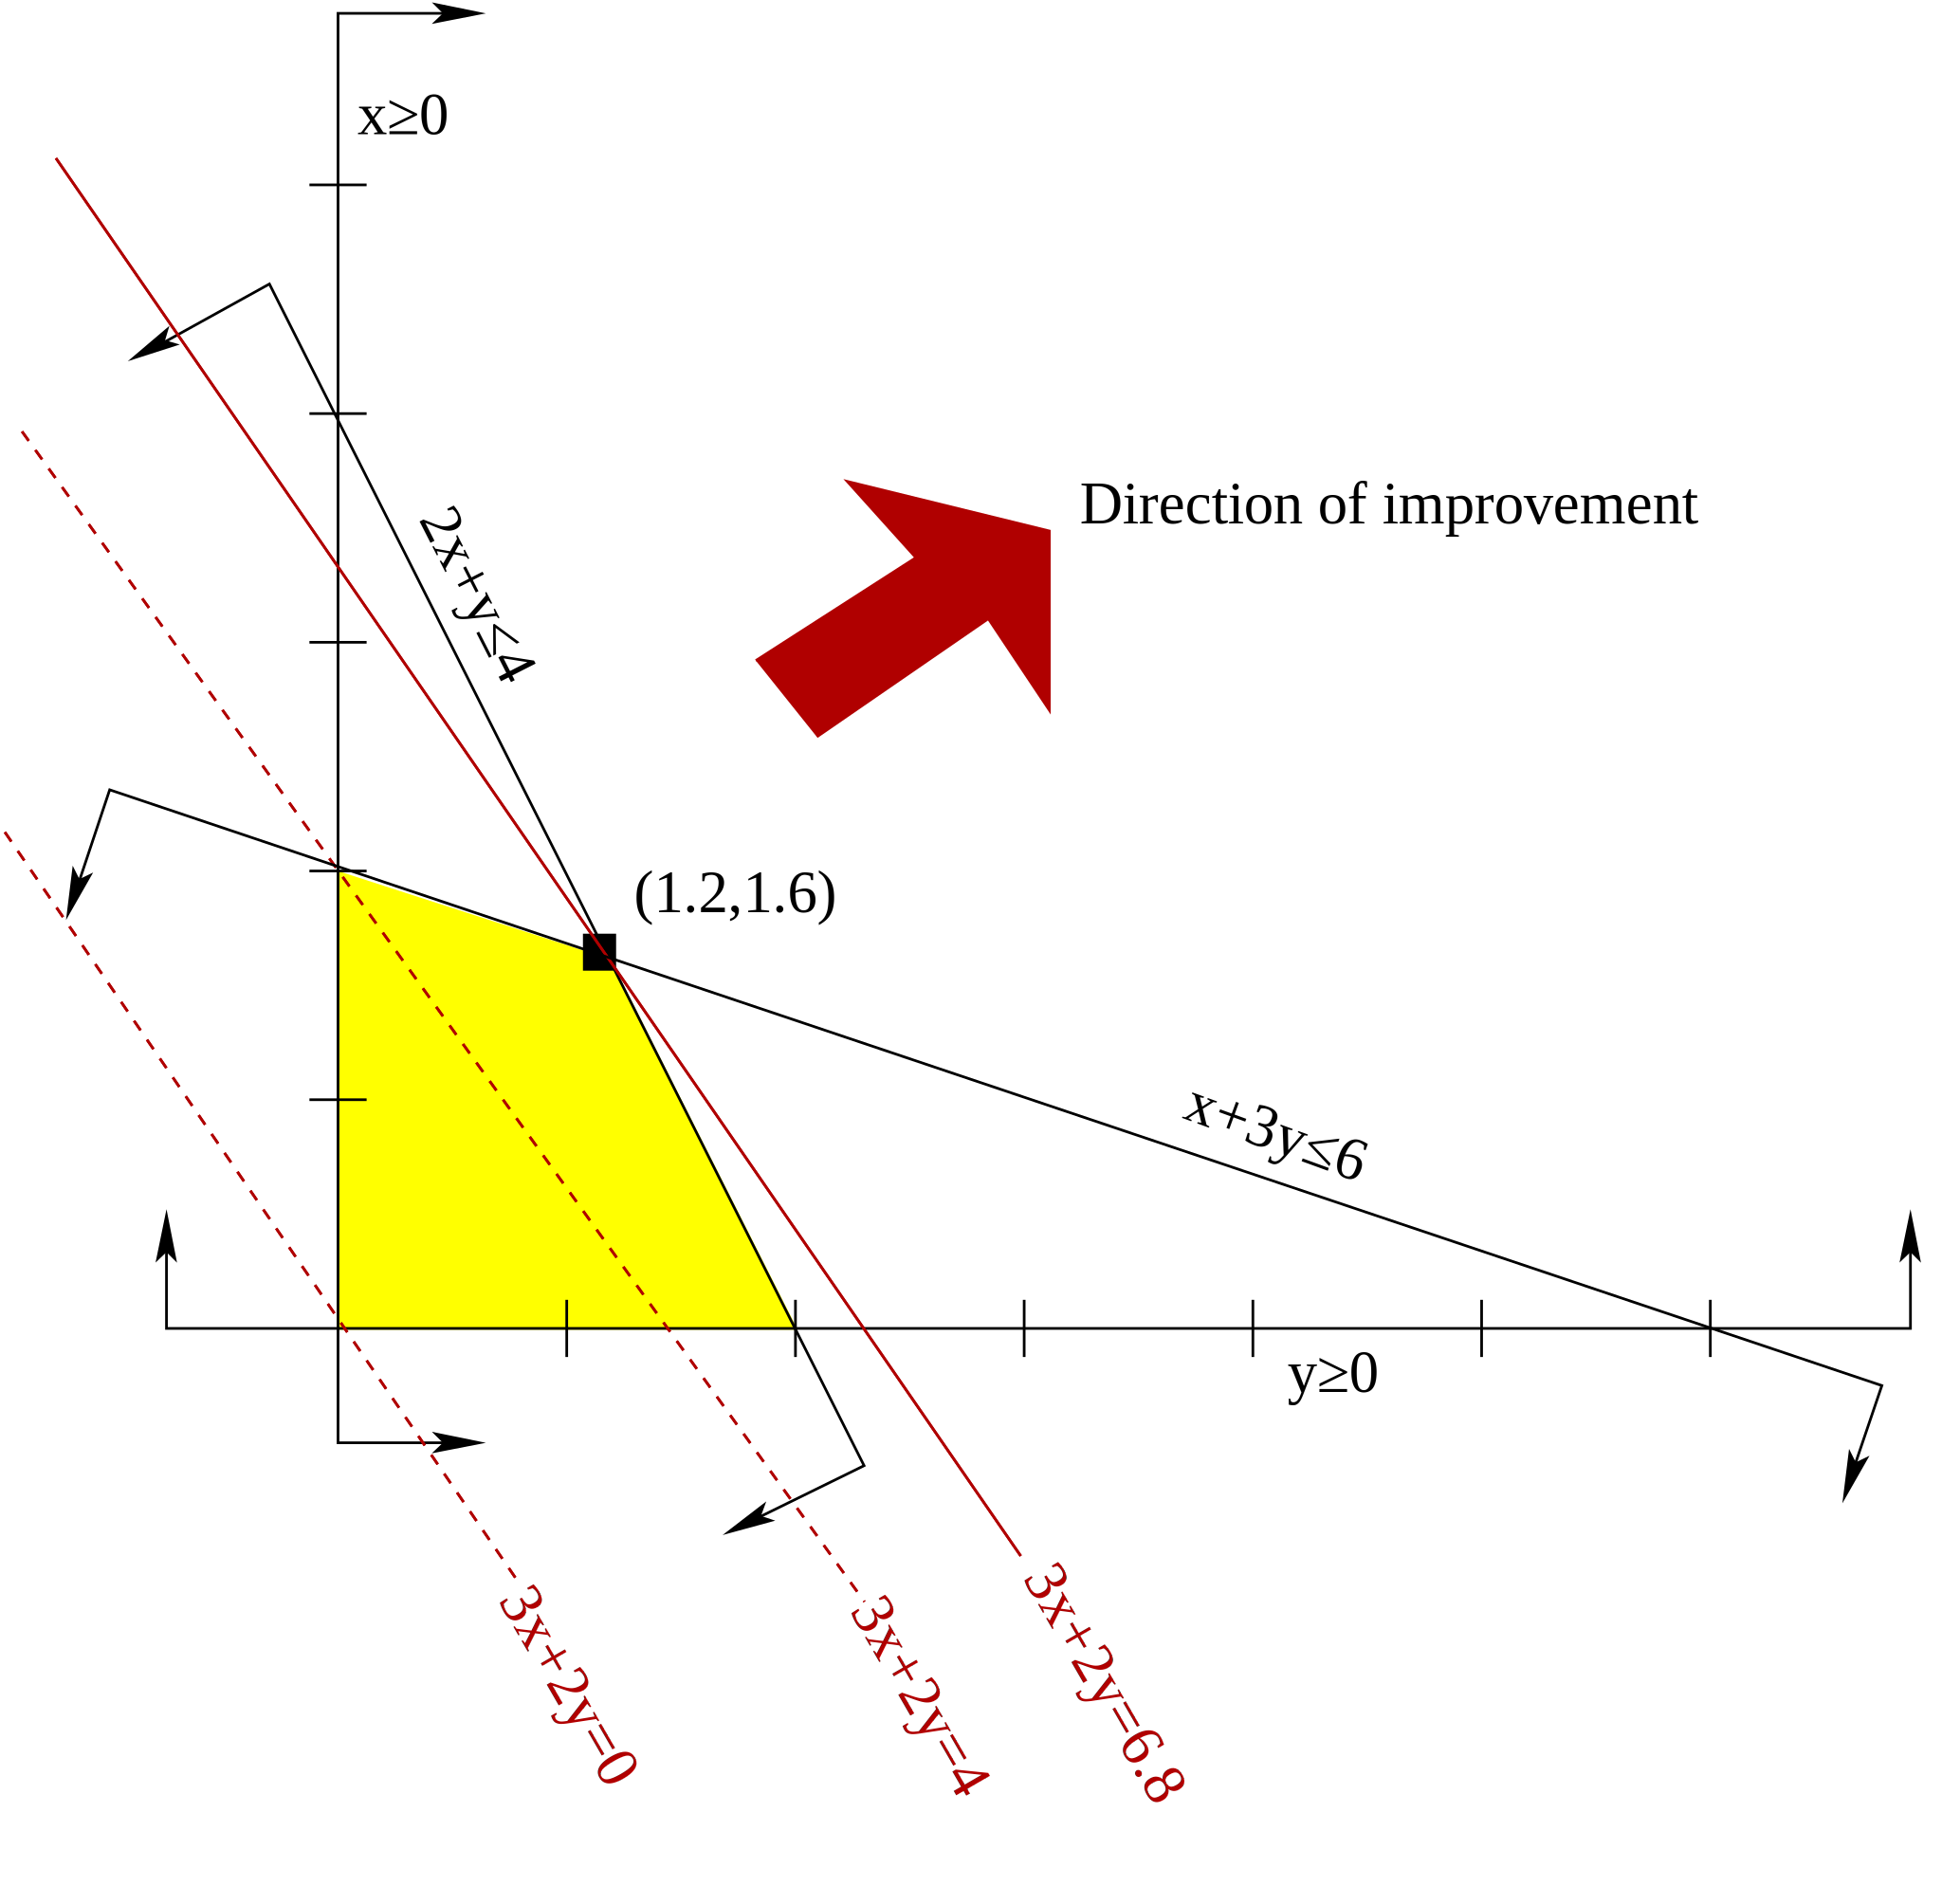
\includegraphics[width=0.8\linewidth]{images/lemon} \end{center}

In the figure above, the lines with \(z\) at 0, 4 and 6.8 have been
drawn. From the picture, we can see that if \(z\) is greater than 6.8,
the line defined by \(3x+2y = z\) will not intersect the feasible
region. Hence, the profit cannot exceed 6.8 dollars.

As the line \(3x+2y = 6.8\) does intersect the feasible region, \(6.8\)
is the maximum value for the objective function. Note that there is only
one point in the feasible region that intersects the line \(3x+2y=6.8\),
namely
\(\begin{bmatrix} x \\ y\end{bmatrix} = \begin{bmatrix} 1.2 \\ 1.6\end{bmatrix}.\)
In other words, to maximize profit, we want to make 1.2 units of
lemonade and 1.6 units of lemon juice.

The above solution method can hardly be regarded as rigorous because we
relied on a picture to conclude that \(3x + 2y \leq 6.8\) for all
\(\begin{bmatrix} x\\y\end{bmatrix}\) satisfying the constraints. But we
can actually show this \emph{algebraically}.

Note that multiplying both sides of the constraint \(x + 3y \leq 6\)
gives \(0.2x + 0.6 y \leq 1.2\), and multiplying both sides of the
constraint \(2x + y \leq 4\) gives \(2.8x + 1.4 y \leq 5.6\). Hence, any
\(\begin{bmatrix} x\\y\end{bmatrix}\) that satisfies both \(x+3y\leq 6\)
and \(2x+y \leq 4\) must also satisfy
\((0.2x+0.6y) + (2.8x+1.4y) \leq 1.2 + 5.6\), which simplifies to
\(3x + 2y \leq 6.8\) as desired! (Here, we used the fact that if
\(a \leq b\) and \(c \leq d\), then \(a+c \leq b+d\).)

Now, one might ask if it is always possible to find an algebraic proof
like the one above for similar problems. If the answer is yes, how does
one find such a proof? We will see answers to this question later on.

Before we end this segment, let us consider the following problem:
\[\begin{array}{rrcrll}
\mbox{minimize } & -2x & + & y & \\
\mbox{subject to} & -x & + & y & \leq & 3 \\
& x & - &  2y & \leq & 2 \\
& x &  & & \geq & 0 \\
& & & y & \geq & 0. \\
\end{array}\]

Note that for any \(t \geq 0\),
\(\begin{bmatrix} x \\ y\end{bmatrix} = \begin{bmatrix} t \\ t\end{bmatrix}\)
satisfies all the constraints. The value of the objective function at
\(\begin{bmatrix} x \\ y\end{bmatrix} = \begin{bmatrix} t \\ t\end{bmatrix}\)
is \(-t\). As \(t \rightarrow \infty\), the value of the objective
function tends to \(-\infty\). Therefore, there is no minimum value for
the objective function. The problem is said to be unbounded. Later on,
we will see how to detect unboundedness algorithmically.

As an exercise, check that unboundedness can also be established by
using
\(\begin{bmatrix} x \\ y\end{bmatrix} = \begin{bmatrix} 2t+2 \\ t\end{bmatrix}\)
for \(t \geq 0\).

\subsection*{Exercises}\label{exercises}
\addcontentsline{toc}{section}{Exercises}

\begin{enumerate}
\def\labelenumi{\arabic{enumi}.}
\item
  Sketch all \(\begin{bmatrix} x \\ y \end{bmatrix}\) satisfying

  \begin{equation*}
  x - 2y \leq 2
  \end{equation*}

  on the \((x,y)\)-plane.
\item
  Determine the optimal value of \[
  \begin{array}{rl}
  \text{Minimize} & x + y \\
  \text{Subject to} &  2x + y \geq 4 \\
  & x + 3y \geq 1.
  \end{array}
  \]
\item
  Show that the problem \[
  \begin{array}{rl}
  \text{Minimize} & -x + y \\
  \text{Subject to} &  2x - y \geq 0 \\
  & x + 3y \geq 3
  \end{array}
  \] is unbounded.
\item
  Suppose that you are shopping for dietary supplements to satisfy your
  required daily intake of 0.40mg of nutrient \(M\) and 0.30mg of
  nutrient \(N\). There are three popular products on the market. The
  costs and the amounts of the two nutrients are given in the following
  table:

  \begin{longtable}[]{@{}lccc@{}}
  \toprule
  & Product 1 & Product 2 & Product 3\tabularnewline
  \midrule
  \endhead
  Cost & \$27 & \$31 & \$24\tabularnewline
  Daily amount of \(M\) & 0.16 mg & 0.21 mg & 0.11 mg\tabularnewline
  Daily amount of \(N\) & 0.19 mg & 0.13 mg & 0.15 mg\tabularnewline
  \bottomrule
  \end{longtable}

  You want to determine how much of each product you should buy so that
  the daily intake requirements of the two nutrients are satisfied at
  minimum cost. Formulate your problem as a linear programming problem,
  assuming that you can buy a fractional number of each product.
\end{enumerate}

\subsection*{Solutions}\label{solutions}
\addcontentsline{toc}{subsection}{Solutions}

\begin{enumerate}
\def\labelenumi{\arabic{enumi}.}
\item
  The points \((x,y)\) satisfying \(x-2y \leq 2\) are precisely those
  above the line passing through \((2,0)\) and \((0,-1)\).
\item
  We want to determine the minimum value \(z\) so that \(x+y=z\) defines
  a line that has a nonempty intersection with the feasible region.
  However, we can avoid referring to a sketch by setting \(x=z-y\) and
  substituting for \(x\) in the inequalities to obtain:

  \begin{eqnarray*}
   2(z-y) + y \geq 4 \\
   (z-y) + 3y \geq 1,
  \end{eqnarray*}

  or equivalently,

  \begin{eqnarray*}
   z \geq 2+\frac{1}{2}y \\
   z \geq 1-2y,
  \end{eqnarray*}

  Thus, the minimum value for \(z\) is
  \(\min \{ 2+\frac{1}{2}y, 1-2y\}\), which occurs at
  \(y = -\frac{2}{5}\). Hence, the optimal value is \(\frac{9}{5}\).

  We can verify our work by doing the following. If our calculations
  above are correct, then an optimal solution is given by
  \(x = \frac{11}{5}\), \(y = -\frac{2}{5}\) since \(x = z - y\). It is
  easy to check that this satisfies both inequalities and therefore is a
  feasible solution.

  Now, taking \(\frac{2}{5}\) times the first inequality and
  \(\frac{1}{5}\) times the second inequality, we can infer the
  inequality \(x+y \geq \frac{9}{5}\). The left-hand side of this
  inequality is precisely the objective function. Hence, no feasible
  solution can have objective function value less than \(\frac{9}{5}\).
  But \(x = \frac{11}{5}\), \(y = -\frac{2}{5}\) is a feasible solution
  with objective function value equal to \(\frac{9}{5}\). As a result,
  it must be an optimal solution.

  \textbf{Remark.} We have not yet discussed how to obtain the
  multipliers \(\frac{2}{5}\) and \(\frac{1}{5}\) for inferring the
  inequality \(x+y \geq \frac{9}{5}\). This is an issue that will be
  taken up later. In the meantime, think about how one could have
  obtained these multipliers for this particular exercise.
\item
  We could glean some insight by first making a sketch on the
  \((x,y)\)-plane.

  The line defined by \(-x + y = z\) has \(x\)-intercept \(-z\). Note
  that for \(z \leq -3\),
  \(\begin{bmatrix} x\\y \end{bmatrix} = \begin{bmatrix} -z\\ 0\end{bmatrix}\)
  satisfies both inequalities and the value of the objective function at
  \(\begin{bmatrix} x\\y \end{bmatrix} = \begin{bmatrix} -z\\ 0\end{bmatrix}\)
  is \(z\). Hence, there is no lower bound on the value of objective
  function.
\item
  Let \(x_i\) denote the amount of Product \(i\) to buy for
  \(i = 1,2,3\). Then, the problem can be formulated as
  \[\begin{array}{rrcrcrll}
  \mbox{minimize } & 27 x_1 & + & 31 x_2 & + & 24 x_3 \\
  \mbox{subject to} 
  & 0.16 x_1 & + & 0.21 x_2 & + & 0.11 x_3 & \geq & 0.30 \\
  & 0.19 x_1 & + & 0.13 x_2 & + & 0.15 x_3 & \geq & 0.40 \\
  & x_1 & , & x_2 & , & x_3 & \geq & 0. \\
  \end{array}\]

  \textbf{Remark.} If one cannot buy fractional amounts of the products,
  the problem can be formulated as \[\begin{array}{rrcrcrll}
  \mbox{minimize } & 27 x_1 & + & 31 x_2 & + & 24 x_3 \\
  \mbox{subject to} 
  & 0.16 x_1 & + & 0.21 x_2 & + & 0.11 x_3 & \geq & 0.30 \\
  & 0.19 x_1 & + & 0.13 x_2 & + & 0.15 x_3 & \geq & 0.40 \\
  & x_1 & , & x_2 & , & x_3 & \geq & 0. \\
  & x_1 & , & x_2 & , & x_3 & \in & \mathbb{Z}. \\
  \end{array}\]
\end{enumerate}


\begin{tikzpicture}
    \draw[gray!50, thin, step=0.5] (-1,-3) grid (5,4);
    \draw[very thick,->] (-1,0) -- (5.2,0) node[right] {$x_1$};
    \draw[very thick,->] (0,-3) -- (0,4.2) node[above] {$x_2$};

    \foreach \x in {-1,...,5} \draw (\x,0.05) -- (\x,-0.05) node[below] {\tiny\x};
    \foreach \y in {-3,...,4} \draw (-0.05,\y) -- (0.05,\y) node[right] {\tiny\y};

    \fill[blue!50!cyan,opacity=0.3] (8/3,1/3) -- (1,2) -- (13/3,11/3) -- cycle;

    \draw (-1,4) -- node[below,sloped] {\tiny$x_1+x_2\geq3$} (5,-2);
    \draw (1,-3) -- (3,1) -- node[below left,sloped] {\tiny$2x_1-x_2\leq5$} (4.5,4);
    \draw (-1,1) -- node[above,sloped] {\tiny$-x_1+2x_2\leq3$} (5,4);

\end{tikzpicture}\footnote{
\url{https://tex.stackexchange.com/questions/75933/how-to-draw-the-region-of-inequality}
}

\fi

%\newcommand\oldstuff{thus}
%
\section{The Simplex Method} {The Simplex Method}
\todoSection{Integrate this to next chapter (chapter on simplex method)}
\label{lab:Simplex}
\objective{
The \emph{Simplex Method} is a straightforward algorithm for finding optimal solutions to optimization problems with linear constraints and cost functions.
Because of its simplicity and applicability, this algorithm has been named one of the most important algorithms invented within the last 100 years.
In this lab we implement a standard Simplex solver for the primal problem. %s that are feasible at the origin.
}

% The algorithm obtains the solution by traversing the edges of the feasible region defined by the constraints.
% The theory of convex optimization guarantees that the optimal point will be found among the vertices of the feasible region, and so a carefully implemented Simplex Algorithm will discover the exact solution in a finite number of steps.

\subsection*{Standard Form} % ====================================================

The Simplex Algorithm accepts a linear constrained optimization problem, also called a \emph{linear program}, in the form given below:

\begin{align*}
\text{minimize}\qquad &\c\trp\x \\
\text{subject to}\qquad & A\x \leq \b \\
 &\x \geq \0
\end{align*}

Note that any linear program can be converted to standard form, so there is no loss of generality in restricting our attention to this particular formulation.

Such an optimization problem defines a region in space called the \emph{feasible region}, the set of points satisfying the constraints.
Because the constraints are all linear, the feasible region forms a geometric object called a \emph{polytope}, having flat faces and edges (see Figure \ref{fig:polytope}).
The Simplex Algorithm jumps among the vertices of the feasible region searching for an optimal point.
It does this by moving along the edges of the feasible region in such a way that the objective function is always increased after each move.

\begin{figure}[H]
\captionsetup[subfigure]{justification=centering}
\centering
\begin{subfigure}{.5\textwidth} % 2-d feasible polytope.
    \centering
    \includegraphics[width=\linewidth]{foundationsAppliedMathematicsLabs/Volume2/Simplex/figures/feasiblePolytope.pdf}
    \caption{The feasible region for a linear program with 2-dimensional constraints.}
\end{subfigure}%
\begin{subfigure}{.5\textwidth} % 3-d feasible polytope.
    \begin{center}
    \begin{tikzpicture}[dot/.style={circle,fill=blue,minimum size=3pt,inner sep=0pt, outer sep=-1pt}, >=stealth']

    \draw[blue!10!, fill=blue!5!](3,1)--(1.5,2.3)--(1.75,1.3)--cycle;
    \draw[blue!25!, fill = blue!15!](3,1)--(1.75,1.3)--(2.3,-1)--cycle;
    \draw[blue!55!, fill = blue!40!](1.75,1.3)--(2.3,-1)--(.8,-1)--cycle;
    \draw[blue!80!, fill = blue!65!](.8,-1)--(-.05,-.2)--(.25,.6)--(1.22,.06)--cycle;
    \draw[blue!85!, fill = blue!73!](-.05, -.2)--(-.3,0)--(.1, 1.65)--(.25, .6)--cycle;
    \draw[blue!65!, fill = blue!50!](.1,1.7)--(.25,.6)--(1.22,.07)--(1.75,1.3)--cycle;
    \draw[blue!40!, fill = blue!15!](.1,1.7)--(1.75,1.3)--(1.5,2.3)--cycle;

    \draw[-,thick](-.3,0)--(.1,1.7)--(1.5, 2.3)--(3, 1)--(2.3,-1)--(.8,-1)--cycle;

    \draw[-,thick](.1,1.7)--(3,1);
    \draw[-,thick](1.5, 2.3)--(2.3,-1);
    \draw[-,thick](.8,-1)--(1.74,1.3);
    \draw[-,thick](.1,1.7)--(.25,.6);
    \draw[-,thick](1.24,.07)--(.25,.6);
    \draw[-,thick](-.05,-.24)--(.25,.6);

    \draw[->](.37,.63)--(.22,1.61);
    \draw[->](.31,1.55)--(1.63,1.23);
    \draw[->](.75,-.85)--(1.12,.05);
    \draw[->](1.05,.05)--(.25,.48);
    \draw[->](1.83,1.35)--(1.65,2.1);

    \node[draw=none](x*)at(1.8,2.45){$\x^*$};

    \end{tikzpicture}
    \end{center}
    \caption{The feasible region for a linear program with 3-dimensional constraints.}
\end{subfigure}
\caption{If an optimal point exists, it is one of the vertices of the polyhedron.
The simplex algorithm searches for optimal points by moving between adjacent vertices in a direction that increases the value of the objective function until it finds an optimal vertex.}
\label{fig:polytope}
\end{figure}

% \begin{figure}[htb] % 3-d feasible polytope.
% \end{figure}


% % TODO: subfigure for 3-d polytope from book.

Implementing the Simplex Algorithm is straightforward, provided one carefully follows the procedure.
We will break the algorithm into several small steps, and write a function to perform each one.
To become familiar with the execution of the Simplex algorithm, it is helpful to work several examples by hand.

\subsection*{The Simplex Solver} % ===============================================

Our program will be more lengthy than many other lab exercises and will consist of a collection of functions working together to produce a final result.
It is important to clearly define the task of each function and how all the functions will work together.
If this program is written haphazardly, it will be much longer and more difficult to read than it needs to be.
We will walk you through the steps of implementing the Simplex Algorithm as a Python class.
% Since the Simplex Algorithm assumes that all the variables are non-negative, we do not need any special logic for it.
% what is this previous statement saying? What 'special logic' would you need if the variables were negative?

For demonstration purposes, we will use the following linear program.
\begin{align*}
\text{minimize}\qquad & -3x_0 - 2x_1 \\
\text{subject to}\qquad
& x_0 - x_1 \leq 2 \\
& 3x_0 + x_1 \leq 5 \\
& 4x_0 + 3x_1 \leq 7 \\
& x_0, x_1 \geq 0.
\end{align*}

\subsection*{Accepting a Linear Program} % ------------------------------------

Our first task is to determine if we can even use the Simplex algorithm.
Assuming that the problem is presented to us in standard form, we need to check that the feasible region includes the origin.  For now, we only check for feasibility at the origin. A more robust solver sets up the auxiliary problem and solves it to find a starting point if the origin is infeasible.

\begin{problem}{Check feasibility at the origin.}{}
Write a class that accepts the arrays $\c$, $A$, and $\b$ of a linear optimization problem in standard form.
In the constructor, check that the system is feasible at the origin.
That is, check that $A\x \preceq \b$ when $\x = \0$. Raise a \li{ValueError} if the problem is not feasible at the origin. \label{prob:initsolver}
\end{problem}

\subsection*{Adding Slack Variables} % ----------------------------------------

The next step is to convert the inequality constraints $A\x \leq \b$ into equality constraints by introducing a slack variable for each constraint equation.
If the constraint matrix $A$ is an $m \times n$ matrix, then there are $m$ slack variables, one for each row of $A$.
Grouping all of the slack variables into a vector $\w$ of length $m$, the constraints now take the form $A\x + \w = \b$.
In our example, we have \[\w = \left[\begin{array}{c}x_2\\x_3 \\x_4\end{array}\right]\]

% TODO: change the representation of the slack variables to match the book.
When adding slack variables, it is useful to represent all of your variables, both the original primal variables and the additional slack variables, in a convenient manner.
One effective way is to refer to a variable by its subscript.
For example, we can use the integers $0$ through $n-1$ to refer to the original (non-slack) variables $x_0$ through $x_{n-1}$, and we can use the integers $n$ through $n+m-1$ to track the slack variables (where the slack variable corresponding to the $i$th row of the constraint matrix is represented by the index $n+i-1$).

We also need some way to track which variables are \emph{independent} (non-zero) and which variables are \emph{dependent} (those that have value $0$). This can be done using the objective function. At anytime during the optimization process, the non-zero variables in the objective function are \emph{independent} and all other variables are \emph{dependent}. 

%A useful representation for the variables is a Python list (or NumPy array), where the elements of the list are integers.
%Since we know how many dependent variables we have ($m$), we can partition the list so that all the dependent variables are kept in the first $m$ locations, and all the independent variables are stored at the end of the list.
%The ordering of this list is important.
%In particular, if $i \leq m$, the $i$th element of the list represents the dependent variable corresponding to the $i$th row of $A$.
%Henceforth we will refer to this list as the \emph{index list}.

%Initially, the dependent variables are simply the slack variables, and their values correspond to the values of %the vector $\b$.
%In our example, we have 2 primal variables $x_0$ and $x_1$, and we must add 3 slack variables.
%Thus, we instantiate the following index list:

%\begin{lstlisting}
%>>> L = [2, 3, 4, 0, 1]
%\end{lstlisting}

%Notice how the first $3$ entries of the index list are $2, 3, 4$, the indices representing the slack variables.
%This reflects the fact that the dependent variables at this point are exactly the slack variables.

%As the Simplex Algorithm progresses, however, the dependent variables change, and it will be necessary to swap
%elements in our index list.
%For example, suppose the variable represented by the index $4$ becomes independent, while the variable %represented by index $0$ becomes dependent.
%In this case we swap these two entries in the index list.

%\begin{lstlisting}
%>>> L[2], L[3] = L[3], L[2]
%>>> L
%[2, 3, 0, 4, 1]
%\end{lstlisting}

%Now our index list tells us that the current dependent variables $2, 3, 0$.

%\begin{problem} % Slack variables. % TODO: this problem is worthless...
%Design and implement a way to store and track all of the dependent and independent variables.

%Hint: Using integers that represent the index of each variable is useful for Problem \ref{prob:blands}.
%\label{prob:slackvars}
%\end{problem}

\subsection*{Creating a Dictionary} % --------------------------------------------

After we have determined that our program is feasible, we need to create the \emph{dictionary} (sometimes called the \emph{tableau}), a matrix to track the state of the algorithm.
%Remember that your dictionary will need to include in some way the slack variables that you created in Problem \ref{prob:slackvars}.

There are many different ways to build your dictionary.
One way is to mimic the dictionary that is often used when performing the Simplex Algorithm by hand. To do this we will set the corresponding dependent variable equations to 0. For example, if $x_5$ were a dependent variable we would expect to see a -1 in the column that represents $x_5$.
Define \[\bar{A} = \left[\begin{array}{cc} A & I_m \end{array}\right],\]
where $I_m$ is the $m \times m$ identity matrix we will use to represent our slack variables, and define
\[\bar{\c} = \left[\begin{array}{c}\c\\ \0\end{array}\right].\]
That is, $\bar{\c} \in \mathbb{R}^{n+m}$ such that the first $n$ entries are $\c$ and the final $m$ entries are zeros.
Then the initial dictionary has the form
\begin{equation}
D =
\left[\begin{array}{ccc}
0  & \bar{\c}\trp \\
\b &  -\bar{A} 
\end{array}\right]
\label{eqn:hand_tab}
\end{equation}

The columns of the dictionary correspond to each of the variables (both primal and slack), and the rows of the dictionary correspond to the dependent variables.
%Using the convention introduced above of representing the variables by indices in the index list, we have the following correspondence:
%\[
%\text{column } i \Leftrightarrow \text{index } i-2, \qquad i = 2, 3, \ldots, n+m+1,
%\]
%and
%\[
%\text{row } j \Leftrightarrow L_{j-1}, \qquad j = 2, 3, \ldots, m+1,
%\]
%where $L_{j-1}$ refers to the $(j-1)$th entry of the index list.

%For our example problem, the initial index list is
%\[
%L = (2, 3, 4, 0, 1),
%\]
For our example the initial dictionary is
\begin{equation*}
D = \begin{bmatrix}
    0 & -3 & -2 & 0 & 0 & 0\\
    2 & -1 & 1 & -1 & 0 & 0\\
    5 & -3 & -1 & 0 & -1 & 0\\
    7 & -4 & -3 & 0 & 0 & -1
    \end{bmatrix}.
\end{equation*}
%The third column corresponds to index $1$, and the fourth row corresponds to index $4$, since this is the
%third entry of the index list.

The advantage of using this kind of dictionary is that it is easy to check the progress of your algorithm by hand.
%The disadvantage is that pivot operations require careful bookkeeping to track the variables and constraints.

% This dictionary is less intuitive, and I think could lead to more confusion.
\begin{comment}
We can also use a dictionary of the format:
\begin{equation}
T = \begin{bmatrix}
    0 & \c\trp  & 0 \\
    \0 & I_n & \0\\
    \b & -A  & \0
\end{bmatrix}.
\label{eqn:matrix_tab}
\end{equation}
Here, $T$ is a square matrix of size $(n+m+1) \times (n+m+1)$.
The advantage of this form of the dictionary is that all the pivot bookkeeping is built into the matrix.
For our example problem, the initial dictionary of this form is
\begin{equation}
T = \begin{bmatrix}
        0 & 3 & 2 & 0 & 0 & 0 \\
        0 & 1 & 0 & 0 & 0 & 0 \\
        0 & 0 & 1 & 0 & 0 & 0 \\
        2 &-1 & 1 & 0 & 0 & 0 \\
        5 &-3 &-1 & 0 & 0 & 0 \\
        7 &-4 &-3 & 0 & 0 & 0
\end{bmatrix}.
\label{eqn:matrix_inittab}
\end{equation}
\end{comment}

\begin{problem}{Initialize the dictionary.}
Add a method to your Simplex solver that takes in arrays c, A, and b to create the initial dictionary (D) as a NumPy array.
\label{prob:makedictionary}
\end{problem}

\subsection{Pivoting} % ------------------------------------------------------

Pivoting is the mechanism that really makes Simplex useful.
Pivoting refers to the act of swapping dependent and independent variables, and transforming the dictionary appropriately.
This has the effect of moving from one vertex of the feasible polytope to another vertex in a way that increases the value of the objective function.
Depending on how you store your variables, you may need to modify a few different parts of your solver to reflect this swapping.

When initiating a pivot, you need to determine which variables will be swapped.
In the dictionary representation, you first find a specific element on which to pivot, and the row and column that contain the pivot element correspond to the variables that need to be swapped.
Row operations are then performed on the dictionary so that the pivot column becomes a negative elementary vector.

Let's break it down, starting with the pivot selection.
We need to use some care when choosing the pivot element.
To find the pivot column, search from left to right along the top row of the dictionary (ignoring the first column), and stop once you encounter the first negative value.
The index corresponding to this column will be designated the \emph{entering index}, since after the full pivot operation, it will enter
the basis and become a dependent variable.

Using our initial dictionary $D$ in the example, we stop at the second column:
\[ D = \left[ \:
\begin{array}{*{7}{c}}
\cline{2-2}
0 & \multicolumn{1}{|c}{-3} & \multicolumn{1}{|c}{-2} & 0 & 0 & 0\\
2 & \multicolumn{1}{|c}{-1} & \multicolumn{1}{|c}{1} & -1 & 0 & 0\\
5 & \multicolumn{1}{|c}{-3} & \multicolumn{1}{|c}{-1} & 0 & -1 & 0\\
7 & \multicolumn{1}{|c}{-4} & \multicolumn{1}{|c}{-3} & 0 & 0 & -1\\
\cline{2-2}
\end{array}
\right] \]
We now know that our pivot element will be found in the second column.
The entering index is thus $1$.

Next, we select the pivot element from among the negative entries in the pivot column (ignoring the entry in the first row).
\emph{If all entries in the pivot column are non-negative, the problem is unbounded and has no solution.}
In this case, the algorithm should terminate.
Otherwise, assuming our pivot column is the $j$th column of the dictionary and that the negative entries of this column are
$D_{i_1, j}, D_{i_2, j}, \ldots, D_{i_k, j}$, we calculate the ratios
\[
\frac{-D_{i_1,0}}{D_{i_1,j}}, \frac{-D_{i_2,0}}{D_{i_2,j}}, \ldots, \frac{-D_{i_k,0}}{D_{i_k,j}},
\]
and we choose our pivot element to be one that minimizes this ratio.
If multiple entries minimize the ratio, then we utilize \emph{Bland's Rule}, which instructs us to choose the entry in the row corresponding to the smallest index (obeying this rule is important, as it prevents the possibility of the algorithm cycling back on itself infinitely).
The index corresponding to the pivot row is designated as the \emph{leaving index}, since after the full pivot operation, it will leave the basis and become a independent variable.

In our example, we see that all entries in the pivot column (ignoring the entry in the first row, of course) are negative, and hence they are all potential choices for the pivot element.
We then calculate the ratios, and obtain
\[
\frac{-2}{-1} = 2,\quad \frac{-5}{-3} = 1.66...,\quad \frac{-7}{-4} = 1.75.
\]
We see that the entry in the third row minimizes these ratios.
Hence, the element in the second column (index 1), third row (index 2) is our designated
pivot element.

\[ D = \left[ \:
\begin{array}{*{7}{c}}

0 & -3 & -2 & 0 & 0 & 0\\
2 & -1 & 1 & -1 & 0 & 0\\\cline{2-2}
5 & \multicolumn{1}{|c}{-3} & \multicolumn{1}{|c}{-1} & 0 & -1 & 0\\\cline{2-2}
7 & -4 & -3 & 0 & 0 & -1\\
\end{array}
\right] \]

\begin{comment}
If we are using the dictionary representation in equation \ref{eqn:matrix_tab}, pivot operations are reduced to a simple matrix equation:
\[T = T + T_m \otimes T_n,\]
where $T_m$ is the column corresponding to the variable entering the basis and $T_n$ is a normalized vector corresponding to the variable leaving the basis.
The result of the equation is the new dictionary.

For example, for the initial dictionary, \ref{eqn:matrix_inittab}, we will demonstrate the first pivot operation.
We can do the entire pivot with a single outer product.
The first pivot should occur with $x_1$ leaving and $x_4$ entering.
In other words, we want to pivot at row $i = 4$ and column $j = 1$ in the dictionary (the indices are offset by one because of the objective function and the row of constraints).

The row corresponding to $x_4$ is
\[
\begin{bmatrix} 5 &-3 &-1 & 0 & 0 & 0\end{bmatrix}.
\]
This represents the equation
\[
x_4 = 5 - 3x_1 - x_2.
\]
Our eventual goal is to solve for $x_1$ and substitute into the remaining rows of the dictionary.
A simple method to accomplish this is to rewrite the equation so that we have zero on the left-hand side:
\[
0 = 5 - 3x_1 - x_2 - x_4.
\]
Now, we can normalize this equation so that the coefficient of $x_1$ is $-1$.
This is always accomplished by dividing the equation by the negative of the coefficient of $x_1$:
\begin{equation}
0 = \frac{5}{3} - x_1 - \frac{1}{3}x_2 - \frac{1}{3}x_4.
\label{eq:zero-equation}
\end{equation}
This is represented by the vector
\[
\begin{bmatrix} 5/3 & -1 & -1/3 & 0 & -1/3 & 0\end{bmatrix}.
\]
Since this left-hand side is zero, I can add any scalar multiple of this equation to any of the equations for $x_i$ and still have an equation for $x_i$.
For example, the equation for $x_5$ is
\[
x_5 = 7 - 4x_1 - 3x_2.
\]
Thus, I can add $-4$ times \eqref{eq:zero-equation} to this equation without changing the left-hand side:
\[ x_5 = 7 - 4x_1 - 3x_2 = 7 - 4x_1 - 3x_2 + -4\left(\frac{5}{3} - x_1 - \frac{1}{3}x_2 - \frac{1}{3}x_4\right) = \frac{1}{3} - \frac{5}{3}x_2 + \frac{4}{3} x_4.
\]
Notice that we end up with an equation that does not include $x_1$ and now has $x_4$, just like we wanted.
In fact, this works in all of our equations, including those for the objective function and even for $x_1$!
Since the coefficient of $x_1$ in \eqref{eq:zero-equation} is $-1$, when we scale it by the coefficient of $x_1$ in any particular row, the $x_1$ cancels out.
\[
T = T + \begin{bmatrix}3 \\ 1 \\ 0 \\ -1 \\ -3 \\ -4\end{bmatrix}\begin{bmatrix} 5/3 & -1 & -1/3 & 0 & -1/3 & 0\end{bmatrix}.
\]
The column vector is just the second column of $T$, which is the column containing the coefficients of $x_1$ in each row.
When we compute this sum, we obtain the dictionary.
\[
T = \begin{bmatrix}
        5 &  0 & 1 & 0 & -1 & 0 \\
        5/3 & 0 &-1/3 & 0 &-1/3 & 0 \\
        0 & 0 & 1 & 0 & 0 & 0 \\
        1/3 & 0 & 4/3 & 0 & 1/3 & 0 \\
        0 & 0 & 0 & 0 & 1 & 0 \\
        1/3 & 0 & -5/3 & 0 & 4/3 & 0
\end{bmatrix}.
\]
\end{comment}
%\begin{problem}
%Write a method that will determine the pivot row and pivot column according to Bland's Rule.
% \begin{comment}
\begin{definition}{Bland's Rule}
Choose the independent variable with the smallest index that has a negative coefficient in the objective function
as the leaving variable.
Choose the dependent variable with the smallest index among all the binding dependent variables.
\end{definition}

Bland's Rule is important in avoiding cycles when performing pivots.
This rule guarantees that a feasible Simplex problem will terminate in a finite number of pivots.% \emph{Hint:} Avoid dividing by zero.
% \end{comment}
%\label{prob:blands}
%\end{problem}

%The next step is to swap the entering and leaving indices in our index list.
%In the example, we determined above that these indices are $0$ and $3$.
%We swap these two elements in our index list,
%and the updated index list is now
%\[
%L = (2, 0, 4, 3, 1),
%\]
%so the dependent variables are now given by the indices $2, 0, 4$.

Finally, we perform row operations on our dictionary in the following way: divide the pivot row by the negative value of the pivot entry.
Then use the pivot row to zero out all entries in the pivot column above and below the pivot entry.
In our example, we first divide the pivot row by -3, and then zero out the two entries above the pivot element and the single entry below it:
\begin{align*}
\begin{bmatrix}
    0 & -3 & -2 & 0 & 0 & 0\\
    2 & -1 & 1 & -1 & 0 & 0\\
    5 & -3 & -1 & 0 & -1 & 0\\
    7 & -4 & -3 & 0 & 0 & -1
    \end{bmatrix} &\rightarrow
\begin{bmatrix}
    0 & -3 & -2 & 0 & 0 & 0\\
    2 & -1 & 1 & -1 & 0 & 0\\
    5/3 & -1 & -1/3 & 0 & -1/3 & 0\\
    7 & -4 & -3 & 0 & 0 & -1
    \end{bmatrix}\rightarrow\\
\begin{bmatrix}
    -5 & 0 & -1 & 0 & 1 & 0\\
    2 & -1 & 1 & -1 & 0 & 0\\
    5/3 & -1 & -1/3 & 0 & -1/3 & 0\\
    7 & -4 & -3 & 0 & 0 & -1
    \end{bmatrix} &\rightarrow
\begin{bmatrix}
    -5 & 0 & -1 & 0 & 1 & 0\\
    1/3 & 0 & -4/3 & 1 & -1/3 & 0\\
    5/3 & -1 & -1/3 & 0 & -1/3 & 0\\
    7 & -4 & -3 & 0 & 0 & -1
    \end{bmatrix}\rightarrow\\
\begin{bmatrix}
    -5 & 0 & -1 & 0 & 1 & 0\\
    1/3 & 0 & 4/3 & -1 & 1/3 & 0\\
    5/3 & -1 & -1/3 & 0 & -1/3 & 0\\
    1/3 & 0 & -5/3 & 0 & 4/3 & -1
    \end{bmatrix}&.
\end{align*}
The result of these row operations is our updated dictionary, and the pivot operation is complete.

\begin{problem}{Pivoting}
Add a method to your solver that checks for unboundedness and performs a single pivot operation from start to completion.
If the problem is unbounded, raise a \li{ValueError}.
\end{problem}

\vspace{2mm}

\subsection{Termination and Reading the Dictionary} % ---------------------------

Up to this point, our algorithm accepts a linear program, adds slack variables, and creates the initial dictionary.
After carrying out these initial steps, it then performs the pivoting operation iteratively until the optimal point is found.
But how do we determine when the optimal point is found? The answer is to look at the top row of the dictionary, which represents the objective function.
More specifically, before each pivoting operation, check whether all of the entries in the top row of the dictionary (ignoring the entry in the first column) are nonnegative.
If this is the case, then we have found an optimal solution, and so we terminate the algorithm.

The final step is to report the solution.
The ending state of the dictionary and index list tells us everything we need to know.
The minimal value attained by the objective function is found in the upper leftmost entry of the dictionary.
The dependent variables all have the value $0$ in the objective function or first row of our dictionary array. The independent variables have values given by the first column of the dictionary.
Specifically, the independent variable whose index is located at the $i$th entry of the index list has the value $T_{i+1, 0}$.

In our example, suppose that our algorithm terminates with the dictionary and index list in the following state:
\[
D = \begin{bmatrix}
-5.2 & 0 & 0 & 0 & 0.2 & 0.6\\
0.6 & 0 & 0 & -1 & 1.4 & -0.8\\
1.6 & -1 & 0 & 0 & -0.6 & 0.2\\
0.2 & 0 & -1 & 0 & 0.8 & -0.6\\
\end{bmatrix}
\]
%\[
%L = (2, 0, 1, 3, 4).
%\]
Then the minimal value of the objective function is $-5.2$.
The independent variables have indices $4, 5$ and have the value $0$.
The dependent variables have indices $3, 1,$ and $2$, and have values $.6, 1.6$, and $.2$, respectively.
In the notation of the original problem statement, the solution is given by
\begin{align*}
x_0 &= 1.6\\
x_1 &= .2.
\end{align*}

\begin{problem}{SimplexSolver.solve()}
Write an additional method in your solver called \li{solve()} that obtains the optimal solution, then returns the minimal value, the dependent variables, and the independent variables.
The dependent and independent variables should be represented as two dictionaries that map the index of the variable to its corresponding value.

For our example, we would return the tuple 

\li{(-5.2, \{0: 1.6, 1: .2, 2: .6\}, \{3: 0, 4: 0\})}.
%The correct format of this tuple is critical, as this tuple of information will be used judge whether or not your solver works!
\end{problem}

\vspace{5mm}

At this point, you should have a Simplex solver that is ready to use.
The following code demonstrates how your solver is expected to behave:

\vspace{5mm}

\begin{lstlisting}
>>> import SimplexSolver

# Initialize objective function and constraints.
>>> c = np.array([-3., -2.])
>>> b = np.array([2., 5, 7])
>>> A = np.array([[1., -1], [3, 1], [4, 3]])

# Instantiate the simplex solver, then solve the problem.
>>> solver = SimplexSolver(c, A, b)
>>> sol = solver.solve()
>>> print(sol)
(-5.2,
 {0: 1.6, 1: 0.2, 2: 0.6},
 {3: 0, 4: 0})
\end{lstlisting}

If the linear program were infeasible at the origin or unbounded, we would expect the solver to alert the user by raising an error.

Note that this simplex solver is \emph{not} fully operational.
It can't handle the case of infeasibility at the origin.
This can be fixed by adding methods to your class that solve the \emph{auxiliary problem}, that of finding an initial feasible dictionary when the problem is not feasible at the origin.
Solving the auxiliary problem involves pivoting operations identical to those you have already implemented, so adding this functionality
is not overly difficult.


\subsection{Exercises}

\paragraph{Exercise $1.0$ (Learn $\mathrm{LT}_{\mathrm{E}} \mathrm{X}$ )}

Learn to use $\operatorname{lt}_{\mathrm{E}} X$ for writing all of your homework solutions. Personally, I use MiKTEX, which is an implementation of $\mathrm{ET} \mathrm{E} \mathrm{X}$ for Windows. Specifically, within MiKTEX I am using pdfteTEX (it only matters for certain things like including graphics and also pdf into a document). I find it convenient to use the editor WinEdt, which is very LATEX friendly. A good book on $\mathrm{ET} \mathrm{T} \mathrm{X}$ is

In A.1 there is a template to get started. Also, there are plenty of tutorials and beginner's guides on the web.

\paragraph{Exercise $1.1$ (Convert to standard form)}

Give an original example (i.e., with actual numbers) to demonstrate that you know how to transform a general linear-optimization problem to one in standard form.

\paragraph{Exercise $1.2$ (Weak Duality example)}

Give an original example to demonstrate the Weak Duality Theorem.

\paragraph{Exercise $1.3$ (Convert to $\leq$ form)}

Describe a general recipe for transforming an arbitrary linear-optimization problem into one in which all of the linear constraints are of $\leq$ type.

\paragraph{Exercise $1.4$ ( $m+1$ inequalities)}

Prove that the system of $m$ equations in $n$ variables $A x=b$ is equivalent to the system $A x \leq b$ augmented by only one additional linear inequality - that is, a total of only $m+1$ inequalities.

\paragraph{Exercise $1.5$ (Weak duality for another form)}

Give and prove a Weak Duality Theorem for

$$
\begin{aligned}
\max \quad c^{\prime} x & \\
A x & \leq b ; \\
x & \geq 0 .
\end{aligned}
$$

HINT: Convert $\left(\mathrm{P}^{\prime}\right)$ to a standard-form problem, and then apply the ordinary Weak Duality Theorem for standard-form problems. \paragraph{Exercise 1.6 (Weak duality for a complicated form)}

Give and prove a Weak Duality Theorem for

$$
\begin{gathered}
\min \quad c^{\prime} x+f^{\prime} w \\
\begin{aligned}
A x+B w & \leq b ; \\
D x &=g ;
\end{aligned} \\
x \geq 0 \quad w \leq 0
\end{gathered}
$$

HINT: Convert $\left(\mathrm{P}^{\prime}\right)$ to a standard-form problem, and then apply the ordinary Weak Duality Theorem for standard-form problems.

\paragraph{Exercise $1.7$ (Weak duality for a complicated form - with MATLAB)}

The MATLAB code below makes and solves an instance of $\left(\mathrm{P}^{\prime}\right)$ from Exercise 1.6. Study the code to see how it is works. Now, extend the code to solve the dual of $\left(\mathrm{P}^{\prime}\right)$. Also, after converting $\left(\mathrm{P}^{\prime}\right)$ to standard form (as indicated in the HINT for Exercise 1.6), use MATLAB to solve that problem and its dual. Make sure that you get the same optimal value for all of these problems.





\subsection{$2.5$ Exercises}

\paragraph{Exercise 2.1 (Dual in AMPL)}

Without changing the file production. dat, use AMPL to solve the dual of the Production Problem example, as described in Section 2.1. You will need to modify production.mod and production.run.

\paragraph{Exercise $2.2$ (Sparse solution for linear equations with AMPL)}

In some application areas, it is interesting to find a "sparse solution" - that is, one with few non-zeros - to a system of equations $A x=b$. It is well known that a 1-norm minimizing solution is a good heuristic for finding a sparse solution. Using AMPL, try this idea out on several large examples, and report on your results.

HINT: To get an interesting example, try generating a random $m \times n$ matrix $A$ of zeros and ones, perhaps $m=50$ equations and $n=500$ variables, maybe with probability $1 / 2$ of an entry being equal to one. Then choose maybe $m / 2$ columns from $A$ and add them up to get $b$. In this way, you will know that there is a solution with only $m / 2$ non-zeros (which is already pretty sparse). Your 1-norm minimizing solution might in fact recover this solution $(\odot)$, or it may be sparser $(\odot \odot)$, or perhaps less sparse $(\odot)$.

\paragraph{Exercise $2.3$ (Bloody AMPL)}

A transportation problem is a special kind of (single-commodity min-cost) networkflow problem. There are certain nodes $v$ called supply nodes which have net supply $b_{v}>0$. The other nodes $v$ are called demand nodes, and they have net supply $b_{v}<0$. There are no nodes with $b_{v}=0$, and all arcs point from supply nodes to demand nodes.

A simplified example is for matching available supply and demand of blood, in types $A, B, A B$ and $O$. Suppose that we have $s_{v}$ units of blood available, in types $v \in\{A, B, A B, O\}$. Also, we have requirements $d_{v}$ by patients of different types $v \in$ $\{A, B, A B, O\}$. It is very important to understand that a patient of a certain type can accept blood not just from their own type. Do some research to find out the compatible blood types for a patient; don't make a mistake - lives depend on this! In this spirit, if your model misallocates any blood in an incompatible fashion, you will receive a grade of $F$ on this problem.

Describe a linear-optimization problem that satisfies all of the patient demand with compatible blood. You will find that type $O$ is the most versatile blood, then both $A$ and $B$, followed by $A B$. Factor in this point when you formulate your objective function, with the idea of having the left-over supply of blood being as versatile as possible.

Using AMPL, set up and solve an example of a blood-distribution problem.

\paragraph{Exercise $2.4$ (Mix it up)}

"I might sing a gospel song in Arabic or do something in Hebrew. I want to mix it up and do it differently than one might imagine." - Stevie Wonder

We are given a set of ingredients $1,2, \ldots, m$ with availabilities $b_{i}$ and per unit costs $c_{i}$. We are given a set of products $j, 2, \ldots, m$ with minimum production requirements $d_{j}$ and per unit revenues $e_{j}$. It is required that product $j$ have at least a fraction of $l_{i j}$ of ingredient $i$ and at most a fraction of $u_{i j}$ of ingredient $i$. The goal is to devise a plan to maximize net profit.

Formulate, mathematically, as a linear-optimization problem. Then, model with AMPL, make up some data, try some computations, and report on your results. Exercise $2.5$ (Task scheduling)


We are given a set of tasks, numbered $1,2, \ldots, n$ that should be completed in the minimum amount of time. For convenience, task 0 is a "start task" and task $n+1$ is an "end task". Each task, except for the start and end task, has a known duration $d_{i}$. For convenience, let $d_{0}:=0$. There are precedences between tasks. Specifically, $\Psi_{i}$ is the set of tasks that must be completed before task $i$ can be started. Let $t_{0}:=0$, and for all other tasks $i$, let $t_{i}$ be a decision variable representing its start time.

Formulate the problem, mathematically, as a linear-optimization problem. The objective should be to minimize the start time $t_{n+1}$ of the end task. Then, model the problem with AMPL, make up some data, try some computations, and report on your results.

\paragraph{Exercise $2.6$ (Investing wisely)}

Almost certainly, Albert Einstein did not say that "compound interest is the most powerful force in the universe."

A company wants to maximize their cash holdings after $T$ time periods. They have an external inflow of $p_{t}$ dollars at the start of time period $t$, for $t=1,2, \ldots, T$. At the start of each time period, available cash can be allocated to any of $K$ different investment vehicles (in any available non-negative amounts). Money allocated to investmentvehicle $k$ at the start of period $t$ must be held in that investment $k$ for all remaining time periods, and it generates income $v_{t, t}^{k}, v_{t, t+1}^{k}, \ldots, v_{t T}^{k}$, per dollar invested. It should be assumed that money obtained from cashing out the investment at the end of the planning horizon (that is, at the end of period $T$ ) is part of $v_{t, T}^{k}$. Note that at the start of time period $t$, the cash available is the external inflow of $p_{t}$, plus cash accumulated from all investment vehicles in prior periods that was not reinvested. Finally, assume that cash held over for one time period earns interest of $q$ percent.

Formulate the problem, mathematically, as a linear-optimization problem. Then, model the problem with AMPL, make up some data, try some computations, and report on your results.






\chapter{Simplex Method}


\begin{definition}{Standard Form}{standardform}
A linear program is in \emph{standard form} if is written as 
\begin{align*}
\max \ \ &c^\top x \\
s.t. \ \ & Ax = b\\
& x \geq 0.
\end{align*}
\end{definition}

\begin{definition}{Extreme Point}{extremepoint}
A point $x$ in a convex set $C$ is called an \emph{extreme point} if it cannot be written as a strict convex combination of other points in $C$.
\end{definition}

\begin{theorem}{Optimal Extreme Point - Bounded Case}{}
Consider a linear optimization problem in standard form.  Suppose that the feasible region is bounded and non-empty. 

Then there exists an optimal solution at an extreme point of the feasible region.
\end{theorem}

\begin{proof}[Proof Sketch]

\end{proof}


% Winston
\begin{definition}{Basic solution}{}
A basic solution to $Ax = b$ is obtained by setting $n-m$ variables equal to $0$ and solving for the values of the remaining $m$ variables.  This assumes that the setting $n-m$ variables equal to 0 yields unique values for the remaining $m$ variables or, equivalently, the columns of the remaining $m$ variables are linearly independent.
\end{definition}

\begin{example}{}{}
Consider the problem
\begin{align*}
\max \quad & Z =-5 X-7 Y  \\ 
\text { s.t. } \quad & X+3 Y \geq 6 \\ 
&5 X+ 2 Y \geq 10 \\ 
&Y  \leq 4 \\ 
&X, Y  \geq 0 
\end{align*}

\begin{center}
\includegraphics[scale = 0.4]{screenshots/example1-feasible-region}
\end{center}

We begin by converting this problem to standard form.  
\begin{align*}
\max \quad & Z =-5 X-7 Y + 0s_1 + 0s_2 + 0 s_3\\ 
\text { s.t. } \quad & X+3 Y - s_1 = 6 \\ 
&5 X+ 2 Y - s_2 = 10 \\ 
&Y  + s_3 = 4 \\ 
&X, Y, s_1, s_2, s_3  \geq 0 
\end{align*}

Thus, we can write this problem in matrix form with 

\begin{align}
\max  & \begin{bmatrix}
-5 \\ -7 \\ 0 \\ 0 \\0
\end{bmatrix}^\top \begin{bmatrix}
X\\Y\\s_1\\s_2\\ s_3
\end{bmatrix}\\
&\begin{bmatrix}
1 & 3 & -1 & 0 & 0 \\
5 & 2 & 0 & -1 & 0\\
0 & 1 & 0 & 0 & 1\\
\end{bmatrix}
\begin{bmatrix}
X \\ Y \\ s_1 \\ s_2 \\ s_3
\end{bmatrix}
= 
\begin{bmatrix}
6 \\ 10 \\ 4
\end{bmatrix}\\
&(X,Y,s_1, s_2, s_3) \geq 0
\end{align}


\end{example}


%Winston
\begin{definition}{Basic feasible solution}{}
Any basic solution in which all the variables are non-negative is a \emph{basic feasible solution}.
\end{definition}

%Winston
\begin{theorem}{BFS iff extreme}{}
A point in the feasible region of an LP is an extreme point if and only if it is a basic feasible solution to the LP.
\end{theorem}

To prove this theorem, we 

%Winston
\begin{theorem}{Representation}{}
Consider an LP in standard form, having bfs $b_1, \dots, b_k$.  Any point $x$ in the LP's feasible region may be written in the form 
$$
x = d + \sum_{i=1}^k \sigma_i b_i
$$
where $d$ is $0$ or a direction of unboundedness and $\sum_{i=1}^k \sigma_i = 1$ and $\sigma_i \geq 0$.
\end{theorem}

% Winston
\begin{theorem}{Optimal bfs}{}
If an LP has an optimal solution, then it has an optimal bfs.
\end{theorem}

\begin{proof}
Let $x$ be an optimal solution.  Then 
$$
x = d + \sum_{i=1}^k \sigma_i b_i
$$
where $d$ is 0 or a direction of unboundeness.  

\begin{itemize}
\item If $c^\top d > 0$, the $x'  = \lambda d + \sum_{i=1}^k \sigma_i b_i$ has bigger objective value for $|lambda > 1$, which is a contradiction since $x$ was optimal. 
\item If $c^\top d < 0$, the $x'' =\sum_{i=1}^k \sigma_i b_i$ has a bigger objective value, which is a contradiction since $x$ was optimal.
\end{itemize}
Thus, we conclude that $c^\top d = 0$.

Since $$c^\top x \geq c^\top b_i$$ for all $i=1, \dots, k$, we can conclude that 
$$
c^\top x = c^\top b_i
$$
for all $i$ such that $\sigma_i > 0$.   Hence, there exists an optimal basic feasible solution.
\end{proof}

\section{Simplex Method}

\section{Finding Feasible Basis}

\underline{\bf Finding an Initial BFS}
When a basic feasible solution is not apparent, we an produce one using {\it artificial variables}.  This {\it artificial} basis is undesirable from the perspective of the original problem, we do not want the artificial variables in our solution, so we penalize them in the objective function, and allow the simplex algorithm to drive them to zero (if possible) and out of the basis.  There are two such methods, the {\bf Big M method} and the {\bf Two-phase method}, which we illustrate below:

\vspace{10mm}  Solve the following LP using the Big M Method and the simplex algorithm:

\begin{align*}
max~~ & z = 9x_1 + 6x_2 \\
s.t.~~
&  3x_1 + 3x_2 \le 9 \\
&  2x_1 - 2x_2 \ge 3 \\
&  2x_1 + 2x_2 \ge 4 \\
& x_1, x_2 \ge 0. \\
\end{align*}

Here is the LP is transformed into standard form by using slack variables $x_3$, $x_4$, and $x_5$, with the required artificial variables $x_6$ and $x_7$, which allow us to easily find an initial basic feasible solution (to the artificial problem).
\begin{eqnarray}
& max  & z_a = 9x_1 + 6x_2 -M x_6 - M x_7 \nonumber \\
& s.t. & 3x_1 + 3x_2 + x_3 = 9 \nonumber \\
&      & 2x_1 - 2x_2 - x_4 + x_6 = 3 \nonumber \\
&      & 2x_1 + 2x_2 - x_5 + x_7 = 4 \nonumber \\
&      & x_i \ge 0,~~ i =1,\cdots,7. \nonumber
\end{eqnarray}

\begin{center} \begin{tabular} {|c|c|c|c|c|c|c|c||c| r} \cline{1-9}
$z$	& $x_1$	& $x_2$	& $x_3$	& $x_4$	& $x_5$	& $x_6$	& $x_7$	& RHS &	ratio \\ \cline{1-9}
1	&	 -9 &	 -6 &	 0 &	  0 &	  0 &	  M &	  M &	0 & \\
0	&	  3 &	  3 &	 1 &	  0 &	  0 &	  0 &	  0 &	9 &	 \\
0	&	  2 &	 -2 &	 0 &	 -1 &	  0 &	  1 &	  0 &	3 & \\
0	&	  2 &	  2 &	 0 &	  0 &	 -1 &	  0 &	  1 &	4 &	 \\
\cline{1-9}
\end{tabular} \end{center}
\noindent This tableau is not in the correct form, it does not represent a basis, the columns for the artificial variables need to be adjusted.

\begin{center} \begin{tabular} {|c|c|c|c|c|c|c|c||c| r} \cline{1-9}
$z$	& $x_1$	  & $x_2$  & $x_3$	& $x_4$	& $x_5$	& $x_6$	& $x_7$	& RHS &	ratio \\ \cline{1-9}
1	& -9 - 4M & -6     &	 0 &	  M &	  M &	  0 &	  0 & -7M &	      \\
0	&	  3   &	     3 &	 1 &	  0 &	  0 &	  0 &	  0 &	9 &	3     \\
0	&	  2   &	    -2 &	 0 &	 -1 &	  0 &	  1 &	  0 &	3 &	3/2   \\
0	&	  2   &	     2 &	 0 &	  0 &	 -1 &	  0 &	  1 &	4 &	2     \\
\cline{1-9}
\end{tabular} \end{center}
\noindent The current solution is not optimal, so $x_1$ enters the basis, and by the ratio test, $x_6$ (an artificial variable) leaves the basis.

\begin{center} \begin{tabular} {|c|c|c|c|c|c|c|c||c| r} \cline{1-9}
$z$	&   $x_1$ & $x_2$   & $x_3$	& $x_4$	& $x_5$	& $x_6$	   & $x_7$	& RHS      & ratio \\
\cline{1-9}
1	&     0   & -15 -4M &	 0 & -9/2 -M &	  M & 9/2 + 2M &	  0 &  27/2 -M &    	\\
0	&	  0   &	     6  &	 1 &	 3/2 &	  0 &	    -3/2 &	  0 &	3/2    & 3/4     \\
0	&	  1   &	    -1  &	 0 &	-1/2 &	  0 &	   1/2 &	  0 &	3/2    & -  	\\
0	&	  0   &	     4  &	 0 &	   1 &	 -1 &	     -1 &	  1 &	  1    & 1/4        	\\ \cline{1-9}
\end{tabular} \end{center}
\noindent The current solution is not optimal, so $x_2$ enters the basis, and by the ratio test, $x_7$ (an artificial variable) leaves the basis.

\begin{center} \begin{tabular} {|c|c|c|c|c|c|c|c||c|r} \cline{1-9}
$z$	&   $x_1$ & $x_2$ & $x_3$ & $x_4$	& $x_5$	& $x_6$	   & $x_7$	& RHS     &	ratio \\
\cline{1-9}
1	&     0   &     0 &	 0    & -3/4    & -15/4 &        - &	  - &  17 1/4 &	   \\
0	&	  0   &	    0 &	 1    &	   0    &	3/2 &	     0 &   -3/2 &	  3   &	-  \\
0	&	  1   &	    0 &	 0    &	-1/4    &  -1/4 &	   1/2 &	1/4 &	  7/4 &	-  	\\
0	&	  0   &	    1 &	 0    &	 1/4    &  -1/4 &	  -1/4 &	1/4 &	  1/4 & 1   \\
\cline{1-9}
\end{tabular} \end{center}
\noindent The current solution is not optimal, so $x_4$ enters the basis, and by the ratio test, $x_2$ leaves the basis.

\begin{center} \begin{tabular} {|c|c|c|c|c|c|c|c||c|r} \cline{1-9}
$z$	&   $x_1$ & $x_2$ & $x_3$ & $x_4$ & $x_5$ & $x_6$ & $x_7$ & RHS     &	ratio \\
\cline{1-9}
1	&     0   &    3  &	 0    & 0     & -9/2  &     - &	    - &  18 &	   \\
0	&	  0   &	    0 &	 1    &	   0  &	  3/2 &	    0 &  -3/2 &	  3     &	-  \\
0	&	  1   &	    1 &	 0    &	0     &  -1/2 &	   0  &	  1/2 &	  2   &	-  	\\
0	&	  0   &	    4 &	 0    &	 1    &  -1   &	  -1 &      1 &	  1    & 1   \\ \cline{1-9}
\end{tabular} \end{center}
\noindent The current solution is not optimal, so $x_5$ enters the basis, and by the ratio test, $x_3$ leaves the basis.

\begin{center} \begin{tabular} {|c|c|c|c|c|c|c|c||c|r} \cline{1-9}
$z$	&   $x_1$ & $x_2$ & $x_3$ & $x_4$ & $x_5$ & $x_6$ & $x_7$ & RHS     &	ratio \\
\cline{1-9}
1	&     0   &    3  &	 3    & 0     & 0  &     - &	    - &  27 &	   \\
0	&	  0   &	    0 &	 2/3  &	  0   &	  1 &	    0 &  -1 &	  2     &	 \\
0	&	  1   &	    1 &	 1/3   &   0  &  0 &	   0  &	  0 &	  3   &  	\\
0	&	  0   &	    4 &	 2/3   &	1 &  0   &	  -1 &     0&	 3    &    \\
\cline{1-9}
\end{tabular} \end{center}
The current solution is optimal! \\

\bigskip Solve the following LP using the Two-phase Method and Simplex Algorithm.
\begin{align*}
max~~ & z = 2x_1 + 3x_2   \\
s.t.~~ 
& 3x_1 + 3x_2 \ge 6  \\
& 2x_1 - 2x_2 \le 2  \\
& -3x_1 + 3x_2 \le 6   \\
& x_1, x_2 \ge 0. 
\end{align*}


%\begin{center} \includegraphics[scale=0.7]{Figs_N/TwoPhase}\end{center}

Here is first phase LP (in standard form), where $x_3$, $x_4$, and $x_5$ are slack variables, and $x_6$ is an artificial variable.
\begin{eqnarray}
& min  & z_a = x_6 \nonumber \\
& s.t. & 3x_1 + 3x_2 - x_3 +x_6 = 6 \nonumber \\
&      & 2x_1 - 2x_2 + x_4 = 2 \nonumber \\
&      & -3x_1 + 3x_2 + x_5 = 6 \nonumber \\
&      & x_i \ge 0,~~ i =1,\cdots,6. \nonumber
\end{eqnarray}
Next, we put the LP into a tableau, which, still is not in the right form for our basic variables ($x_6$, $x_4$, and $x_5$).
\begin{center} \begin{tabular} {|c|c|c|c|c|c|c||c| r} \cline{1-8}
$z$	& $x_1$	& $x_2$	& $x_3$	& $x_4$	& $x_5$	& $x_6$	&  RHS & ratio \\ \cline{1-8}
1	&	  0 &	  0 &	 0 &	  0 &	  0 &	 -1 &    0 & \\
0	&	  3 &	  3 &	-1 &	  0 &	  0 &	  1 &	 6 & \\
0	&	  2 &	 -2 &	 0 &	  1 &	  0 &	  0 &	 2 & \\
0	&	  -3 &	  3 &	 0 &	  0 &	  1 &	  0 &	 6 & \\ \cline{1-8}
\end{tabular} \end{center}
To remedy this, we use row operation to modify the row 0 coefficients, yielding the following:
\begin{center} \begin{tabular} {|c|c|c|c|c|c|c||c| r} \cline{1-8}
$z$	& $x_1$	& $x_2$	& $x_3$	& $x_4$	& $x_5$	& $x_6$	&  RHS & ratio \\ \cline{1-8}
1	&	  3 &	  3 &	 -1 &	  0 &	  0 &	  0 &    6 &   \\
0	&	  3 &	  3 &	-1 &	  0 &	  0 &	  1 &	 6 &  2 \\
0	&	  2 &	 -2 &	 0 &	  1 &	  0 &	  0 &	 2 &  - \\
0	&	  -3 &	  3 &	 0 &	  0 &	  1 &	  0 &	 6 &  2 \\ \cline{1-8}
\end{tabular} \end{center}
The current solution is not optimal, either $x_1$ or $x_2$ can enter the basis, let's choose $x_2$. Then by the ratio test, either $x_6$ (an artificial variable) or $x_5$ (a slack variable) can leaves the basis.  Let's choose $x_6$.
\begin{center} \begin{tabular} {|c|c|c|c|c|c|c||c| r} \cline{1-8}
$z$	& $x_1$	& $x_2$	& $x_3$	& $x_4$	& $x_5$	& $x_6$	&  RHS & ratio \\ \cline{1-8}
1	&	  0 &	  0 &	 0 &	  0 &	  0 &  -1 &    0 & \\
0	&	  1 &	  1 &	-1/3 &	  0 &	  0 &   1/3 &	 2 & \\
0	&	  4 &	  0 &	-2/3 &	  1 &	  0 &   2/3 &	 6 & \\
0	&	 -6 &	  0 &	 1 &	  0 &	  1 &	 -1 &	 0 & \\ \cline{1-8}
\end{tabular} \end{center}
The current solution is optimal, so we end the first phase with a basic feasible solution to the original problem, with $x_2$, $x_4$, and $x_5$ as the basic variables.  Now we provide a new row zero that corresponds to the original problem.

\begin{center} \begin{tabular} {|c|c|c|c|c|c|c||c| r} \cline{1-8}
$z$	& $x_1$	& $x_2$	& $x_3$	& $x_4$	& $x_5$	& $x_6$	&  RHS & ratio \\ \cline{1-8}
1	&	  1 &	  0 &	 -1 &	  0 &	  0 &	  0 &   6 & \\
0	&	  1 &	  1 &	-1/3 &	  0 &	  0 &	  1/3 &	 2 &   \\
0	&	  4 &	  0 &	-2/3 &	  1 &	  0 &	  2/3 &	 6 &  \\
0	&	 -6 &	  0 &	 1 &	  0 &	  1 &	  -1 &	 0 &  \\ \cline{1-8}
\end{tabular} \end{center}

\begin{center} \begin{tabular} {|c|c|c|c|c|c|c||c| r} \cline{1-8}
$z$	& $x_1$	& $x_2$	& $x_3$	& $x_4$	& $x_5$	& $x_6$	&  RHS & ratio \\ \cline{1-8}
1	&	 -5 &	  0 &	  0 &	  0 &	  1 &	  -1 &   6 & \\
0	&	 -1 &	  1 &	  0 &	  0 &	1/3 &	  0 &	 2 &   \\
0	&	  0 &	  0 &	  0 &	  1 &	2/3 &	  0 &	 6 &  \\
0	&	 -6 &	  0 &	  1 &	  0 &	  1 &	  -1 &	 0 &  \\ \cline{1-8}
\end{tabular} \end{center}
From this tableau we can see that the LP is unbounded and an extreme point is [0, 2, 0, 6,0] and an extreme direction is [1, 1, 6, 0, 0].




\underline{\bf Degeneracy and the Simplex Algorithm}
\begin{comment}
$\mathbf {n} \cdot (\mathbf {r} -\mathbf {r} _{0})=0.$
(The dot here means a dot (scalar) product.) Expanded this becomes

$a(x-x_{0})+b(y-y_{0})+c(z-z_{0})=0$
which is the point-normal form of the equation of a plane.  This is just a linear equation

$ax+by+cz+d=0$,
where

$d=-(ax_{0}+by_{0}+cz_{0}).$  
Conversely, it is easily shown that if a, b, c and d are constants and a, b, and c are not all zero, then the graph of the equation

$ax+by+cz+d=0$ is a plane having the vector 

$\mathbf{ n} = (a, b, c)$ as a normal. 

This plane can also be described by the "point and a normal vector" prescription above. A suitable normal vector is given by the cross product
${\mathbf {n}}=({\mathbf {p}}_{2}-{\mathbf {p}}_{1})\times ({\mathbf {p}}_{3}-{\mathbf {p}}_{1})$,

and the point r0 can be taken to be any of the given points p1,p2 or p3[6] (or any other point in the plane).
Let p1=(x1, y1, z1), p2=(x2, y2, z2), and p3=(x3, y3, z3) be non-collinear points.

${\displaystyle \mathbf {w\times v} ={\begin{vmatrix}\mathbf {i} &\mathbf {j} &\mathbf {k} \\w_{1}&w_{2}&w_{3}\\v_{1}&v_{2}&v_{3}\\\end{vmatrix}}}$

${\displaystyle {\begin{aligned}\mathbf {w\times v} &={\begin{vmatrix}w_{2}&w_{3}\\v_{2}&v_{3}\end{vmatrix}}\mathbf {i} -{\begin{vmatrix}w_{1}&w_{3}\\v_{1}&v_{3}\end{vmatrix}}\mathbf {j} +{\begin{vmatrix}w_{1}&w_{2}\\v_{1}&v_{2}\end{vmatrix}}\mathbf {k} \\&=(w_{2}v_{3}-w_{3}v_{2})\mathbf {i} +(w_{3}v_{1}-w_{1}v_{3})\mathbf {j} +(w_{1}v_{2}-w_{2}v_{1})\mathbf {k} ,\end{aligned}}}$
\end{comment}

Degeneracy must be considered in the simplex algorithm, as it causes some trouble.  For instance, it might mislead us into thinking there are multiple optimal solutions, or provide faulty insight.  Further, the algorithm as described can {\it cycle}, that is, remain on a degenerate extreme point repeatedly cycling through a subset of bases that represent that point, never leaving. 

\begin{center} \begin{tabular} {c|c|c|c|c|c|c|c|c|c|} \cline{2-10}
min &$z$	& $x_1$ & $x_2$ & $x_3$	& $x_4$	&  $x_5 $& $x_6$ & $x_7$ & $rhs$ \\ \cline{2-10}
       &1		& 0 		  & 0         &	 0 	    &	  3/4     &   -20 & 1/2 & -6  &     0    \\ \cline{2-10}
       &0		&	 1       &	    0   &	 0 			&	  1/4 		&	-8 & -1 &   9 &   0	  \\
       &0		&	 0     &	    1      &	 0 		&	  1 /2		&	 -12 & -1/2 & 3 & 0   \\ 
       &0		&	 0     &	    0      &	 1 		&	  0		&	 0 & 1 & 0 &1   \\ \cline{2-10}
\end{tabular} \end{center}


\bigskip  Solve the following LP using the Simplex Algorithm:
\begin{eqnarray}
& \max  & z = 40x_1 + 30x_2 \nonumber \\
& s.t. & 6x_1 + 4x_2 \le 40 \nonumber \\
&      & 4x_1 + 2x_2 \le 20 \nonumber \\
&      & x_1, x_2 \ge 0. \nonumber
\end{eqnarray}

By adding slack variables, we have the following tableau.
\begin{table}[h!] \begin{center} \begin{tabular} {|c|c|c|c|c||c|}
\hline
$z$ & $x_1$ & $x_2$ & $s_1$ & $s_2$ & RHS \\ \hline
  1 & -40 & -30 & 0   & 0   & 0  \\
  0 &   6 &   4 & 1   & 0   & 40 \\
  0 &   4 &   2 & 0   & 1   & 20 \\ \hline
\end{tabular} \end{center} \end{table}
Luckily, this tableau represents a basis, where BV=$\{s_1, s_2\}$, but by inspecting the row 0 (objective function row) coefficients, we can see that this is not optimal. By Dantzig's Rule, we enter $x_1$ into the basis, and by the ratio test we see that $s_2$ leaves the basis.  By performing elementary row operations, we obtain the following tableau for
the new basis BV=$\{s_1, x_1\}$.
\begin{center} \begin{tabular} {|c|c|c|c|c||c|} \hline
$z$ & $x_1$ & $x_2$ & $s_1$ & $s_2$ & RHS \\
\hline
  1 &     0 &   -10 & 0     &    10 & 200 \\
  0 &     0 &     1 & 1     &  -3/2 & 10 \\
  0 &     1 &   1/2 & 0     &   1/4 &  5 \\
\hline
\end{tabular} \end{center}

This tableau is not optimal, entering $x_2$ into the basis can improve the objective function value. The basic variables $s_1$ and $x_1$ tie in the ration test.  If we have $x_1$ leave the basis, we get the following tableau (BV=$\{s_1, x_2\}$).
\begin{center} \begin{tabular} {|c|c|c|c|c||c|}
\hline
$z$ & $x_1$ & $x_2$ & $s_1$ & $s_2$ & RHS \\
\hline
  1 &    20 &     0 &     0 &    15 & 300 \\
  0 &    -2 &     0 &     1 &    -2 &  0 \\
  0 &     2 &     1 &     0 &   1/2 &  10 \\ \hline
\end{tabular} \end{center}
This is an optimal tableau, with an objective function value of 300,  If instead of $x_1$ leaving the basis, suppose $s_1$ left, this would lead to the following tableau (BV=$\{x_2, x_1\}$).
\begin{center} \begin{tabular} {|c|c|c|c|c||c|} \hline
$z$ & $x_1$ & $x_2$ & $s_1$ & $s_2$ & RHS \\
\hline
  1 &     0 &     0 &    10 &    -5 & 300 \\
  0 &     0 &     1 &     1 &  -3/2 &  10 \\
  0 &     1 &     0 &  -1/2 &     1 &   0 \\ \hline
\end{tabular} \end{center}
This tableau does not look optimal, yet the objective function value is the same as the optimal solution's. This occurs because the optimal extreme point is a degenerate.% as the following figure shows.




\chapter{Duality}

% Copyright 2022 by Robert Hildebrand
%This work is licensed under a
%Creative Commons Attribution-ShareAlike 4.0 International License (CC BY-SA 4.0)
%See http://creativecommons.org/licenses/by-sa/4.0/

\chapter{Duality}
\todoChapter{ {\color{gray}0\% complete. Goal 80\% completion date: January 20, 2023}\\
Notes: This is a borrowed section.  Likely we should update this to match out CC-BY-SA 4.0 license.  Also, update all content to match notation in the book.}

% this was borrowed from \url{https://www.cs.purdue.edu/homes/egrigore/580FT15/26-lp-jefferickson.pdf}
%26.5 Duality Example
Before I prove the stronger duality theorem, let me first provide some intuition about where this duality thing comes from in the first place. ${ }^{6}$ Consider the following linear programming problem:
\begin{align*}
\text { maximize } & 
4 x_{1}+x_{2}+3 x_{3} \\
\text { subject to } \quad x_{1}+4 x_{2} & \leq 2 \\
& 3 x_{1}-x_{2}+x_{3} & \leq 4 \\
& x_{1}, x_{2}, x_{3} & \geq 0
\end{align*}
Let $\sigma^{*}$ denote the optimum objective value for this LP. The feasible solution $x=(1,0,0)$ gives us a lower bound $\sigma^{*} \geq 4$. A different feasible solution $x=(0,0,3)$ gives us a better lower bound $\sigma^{*} \geq 9$. We could play this game all day, finding different feasible solutions and getting ever larger lower bounds. How do we know when we're done? Is there a way to prove an upper bound on $\sigma^{*}$ ?

In fact, there is. Let's multiply each of the constraints in our LP by a new non-negative scalar value $y_{i}$ :
$$
\begin{aligned}
\text { maximize } 4 x_{1}+x_{2}+3 x_{3} & \\
\text { subject to } y_{1}\left(x_{1}+4 x_{2} \quad\right.& \leq 2 y_{1} \\
y_{2}\left(3 x_{1}-x_{2}+x_{3}\right) & \leq 4 y_{2} \\
x_{1}, x_{2}, x_{3} & \geq 0
\end{aligned}
$$
Because each $y_{i}$ is non-negative, we do not reverse any of the inequalities. Any feasible solution $\left(x_{1}, x_{2}, x_{3}\right)$ must satisfy both of these inequalities, so it must also satisfy their sum:
$$
\left(y_{1}+3 y_{2}\right) x_{1}+\left(4 y_{1}-y_{2}\right) x_{2}+y_{2} x_{3} \leq 2 y_{1}+4 y_{2} \text {. }
$$
Now suppose that each $y_{i}$ is larger than the $i$ th coefficient of the objective function:
$$
y_{1}+3 y_{2} \geq 4, \quad 4 y_{1}-y_{2} \geq 1, \quad y_{2} \geq 3 \text {. }
$$
This assumption lets us derive an upper bound on the objective value of any feasible solution:
$$
4 x_{1}+x_{2}+3 x_{3} \leq\left(y_{1}+3 y_{2}\right) x_{1}+\left(4 y_{1}-y_{2}\right) x_{2}+y_{2} x_{3} \leq 2 y_{1}+4 y_{2} .
$$
In particular, by plugging in the optimal solution $\left(x_{1}^{*}, x_{2}^{*}, x_{3}^{*}\right)$ for the original LP, we obtain the following upper bound on $\sigma^{*}$ :
$$
\sigma^{*}=4 x_{1}^{*}+x_{2}^{*}+3 x_{3}^{*} \leq 2 y_{1}+4 y_{2} .
$$
Now it's natural to ask how tight we can make this upper bound. How small can we make the expression $2 y_{1}+4 y_{2}$ without violating any of the inequalities we used to prove the upper bound? This is just another linear programming problem.
$$
\begin{array}{rr}
\text { minimize } & 2 y_{1}+4 y_{2} \\
\text { subject to } & y_{1}+3 y_{2} \geq 4 \\
& 4 y_{1}-y_{2} \geq 1 \\
y_{2} & \geq 3 \\
y_{1}, y_{2} & \geq 0
\end{array}
$$
"This example is taken from Robert Vanderbei's excellent textbook Linear Programming: Foundations and Extensions [Springer, 2001], but the idea appears earlier in Jens Clausen's 1997 paper 'Teaching Duality in Linear Programming: The Multiplier Approach'.

\url{https://www.cs.purdue.edu/homes/egrigore/580FT15/26-lp-jefferickson.pdf}




%Stanford University - CS261: Optimization

%Handout 6

%Luca Trevisan

%January 20, 2011

%\section{Lecture 6}

In which we introduce the theory of duality in linear programming.

\section{The Dual of Linear Program}

Suppose that we have the following linear program in maximization standard form:

$$
\begin{array}{ll}
\underset{n a x i m i z e}{\operatorname{maxim}} & x_{1}+2 x_{2}+x_{3}+x_{4} \\
\text { subject to } & \\
& x_{1}+2 x_{2}+x_{3} \leq 2 \\
& x_{2}+x_{4} \leq 1 \\
& x_{1}+2 x_{3} \leq 1 \\
& x_{1} \geq 0 \\
& x_{2} \geq 0 \\
& x_{3} \geq 0
\end{array}
$$

and that an LP-solver has found for us the solution $x_{1}:=1, x_{2}:=\frac{1}{2}, x_{3}:=0, x_{4}:=\frac{1}{2}$ of cost 2.5. How can we convince ourselves, or another user, that the solution is indeed optimal, without having to trace the steps of the computation of the algorithm?

Observe that if we have two valid inequalities

$$
a \leq b \text { and } c \leq d
$$

then we can deduce that the inequality

$$
a+c \leq b+d
$$

(derived by "summing the left hand sides and the right hand sides" of our original inequalities) is also true. In fact, we can also scale the inequalities by a positive multiplicative factor before adding them up, so for every non-negative values $y_{1}, y_{2} \geq 0$ we also have 

$$
y_{1} a+y_{2} c \leq y_{1} b+y_{2} d
$$

Going back to our linear program (1), we see that if we scale the first inequality by $\frac{1}{2}$, add the second inequality, and then add the third inequality scaled by $\frac{1}{2}$, we get that, for every $\left(x_{1}, x_{2}, x_{3}, x_{4}\right)$ that is feasible for (1),

$$
x_{1}+2 x_{2}+1.5 x_{3}+x_{4} \leq 2.5
$$

And so, for every feasible $\left(x_{1}, x_{2}, x_{3}, x_{4}\right)$, its cost is

$$
x_{1}+2 x_{2}+x_{3}+x_{4} \leq x_{1}+2 x_{2}+1.5 x_{3}+x_{4} \leq 2.5
$$

meaning that a solution of cost $2.5$ is indeed optimal.

In general, how do we find a good choice of scaling factors for the inequalities, and what kind of upper bounds can we prove to the optimum?

Suppose that we have a maximization linear program in standard form.

$$
\begin{array}{ll}
\operatorname{maximize} & c_{1} x_{1}+\ldots c_{n} x_{n} \\
\text { subject to } & \\
& a_{1,1} x_{1}+\ldots+a_{1, n} x_{n} \leq b_{1} \\
& \vdots \\
& a_{m, 1} x_{1}+\ldots+a_{m, n} x_{n} \leq b_{m} \\
& x_{1} \geq 0 \\
& \vdots \\
& x_{n} \geq 0
\end{array}
$$

For every choice of non-negative scaling factors $y_{1}, \ldots, y_{m}$, we can derive the inequality

$$
\begin{gathered}
y_{1} \cdot\left(a_{1,1} x_{1}+\ldots+a_{1, n} x_{n}\right) \\
+\cdots \\
+y_{n} \cdot\left(a_{m, 1} x_{1}+\ldots+a_{m, n} x_{n}\right) \\
\leq y_{1} b_{1}+\cdots y_{m} b_{m}
\end{gathered}
$$

which is true for every feasible solution $\left(x_{1}, \ldots, x_{n}\right)$ to the linear program (2). We can rewrite the inequality as

$$
\begin{aligned}
\left(a_{1,1} y_{1}+\right.&\left.\cdots a_{m, 1} y_{m}\right) \cdot x_{1} \\
+& \cdots
\end{aligned}
$$

 

$$
\begin{gathered}
+\left(a_{1, n} y_{1} \cdots a_{m, n} y_{m}\right) \cdot x_{n} \\
\leq y_{1} b_{1}+\cdots y_{m} b_{m}
\end{gathered}
$$

So we get that a certain linear function of the $x_{i}$ is always at most a certain value, for every feasible $\left(x_{1}, \ldots, x_{n}\right)$. The trick is now to choose the $y_{i}$ so that the linear function of the $x_{i}$ for which we get an upper bound is, in turn, an upper bound to the cost function of $\left(x_{1}, \ldots, x_{n}\right)$. We can achieve this if we choose the $y_{i}$ such that

$$
\begin{aligned}
&c_{1} \leq a_{1,1} y_{1}+\cdots a_{m, 1} y_{m} \\
&\vdots \\
&c_{n} \leq a_{1, n} y_{1} \cdots a_{m, n} y_{m}
\end{aligned}
$$

Now we see that for every non-negative $\left(y_{1}, \ldots, y_{m}\right)$ that satisfies (3), and for every $\left(x_{1}, \ldots, x_{n}\right)$ that is feasible for $(2)$,

$$
\begin{gathered}
c_{1} x_{1}+\ldots c_{n} x_{n} \\
\leq\left(a_{1,1} y_{1}+\cdots a_{m, 1} y_{m}\right) \cdot x_{1} \\
+\cdots \\
+\left(a_{1, n} y_{1} \cdots a_{m, n} y_{m}\right) \cdot x_{n} \\
\leq y_{1} b_{1}+\cdots y_{m} b_{m}
\end{gathered}
$$

Clearly, we want to find the non-negative values $y_{1}, \ldots, y_{m}$ such that the above upper bound is as strong as possible, that is we want to

$$
\begin{array}{ll}
\operatorname{minimize} & b_{1} y_{1}+\cdots b_{m} y_{m} \\
\text { subject to } & \\
& a_{1,1} y_{1}+\ldots+a_{m, 1} y_{m} \geq c_{1} \\
& \vdots \\
& a_{n, 1} y_{1}+\ldots+a_{m, n} y_{m} \geq c_{n} \\
& y_{1} \geq 0 \\
& \vdots \\
& y_{m} \geq 0
\end{array}
$$

So we find out that if we want to find the scaling factors that give us the best possible upper bound to the optimum of a linear program in standard maximization form, we end up with a new linear program, in standard minimization form. Definition 1 If

$$
\begin{array}{ll}
\underset{\text { maximize }}{ } & \mathbf{c}^{T} \mathbf{x} \\
\text { subject to } & \\
& A \mathbf{x} \leq \mathbf{b} \\
& \mathbf{x} \geq \mathbf{0}
\end{array}
$$

is a linear program in maximization standard form, then its dual is the minimization linear program

$$
\begin{array}{ll}
\operatorname{minimize} & \mathbf{b}^{T} \mathbf{y} \\
\text { subject to } & \\
& A^{T} \mathbf{y} \geq \mathbf{c} \\
& \mathbf{y} \geq \mathbf{0}
\end{array}
$$

So if we have a linear program in maximization linear form, which we are going to call the primal linear program, its dual is formed by having one variable for each constraint of the primal (not counting the non-negativity constraints of the primal variables), and having one constraint for each variable of the primal (plus the nonnegative constraints of the dual variables); we change maximization to minimization, we switch the roles of the coefficients of the objective function and of the right-hand sides of the inequalities, and we take the transpose of the matrix of coefficients of the left-hand side of the inequalities.

The optimum of the dual is now an upper bound to the optimum of the primal. How do we do the same thing but starting from a minimization linear program? We can rewrite

$$
\begin{array}{ll}
\underset{l}{\operatorname{minimize}} & \mathbf{c}^{T} \mathbf{y} \\
\text { subject to } & \\
& A \mathbf{y} \geq \mathbf{b} \\
& \mathbf{y} \geq \mathbf{0}
\end{array}
$$

in an equivalent way as

$$
\begin{array}{ll}
\underset{\operatorname{maximize}}{\operatorname{mubject~to}} & -\mathbf{c}^{T} \mathbf{y} \\
& -A \mathbf{y} \leq-\mathbf{b} \\
& \mathbf{y} \geq \mathbf{0}
\end{array}
$$

If we compute the dual of the above program we get

$$
\begin{array}{ll}
\underset{\text { minimize }}{\operatorname{mubject} \text { to }} & -\mathbf{b}^{T} \mathbf{z} \\
& -A^{T} \mathbf{z} \geq-\mathbf{c} \\
& \mathbf{z} \geq \mathbf{0}
\end{array}
$$

that is,

$$
\begin{array}{ll}
\operatorname{maximize} & \mathbf{b}^{T} \mathbf{z} \\
\text { subject to } & \\
& A^{T} \mathbf{z} \leq \mathbf{c} \\
& \mathbf{y} \geq \mathbf{0}
\end{array}
$$

So we can form the dual of a linear program in minimization normal form in the same way in which we formed the dual in the maximization case:

- switch the type of optimization,

- introduce as many dual variables as the number of primal constraints (not counting the non-negativity constraints),

- define as many dual constraints (not counting the non-negativity constraints) as the number of primal variables.

- take the transpose of the matrix of coefficients of the left-hand side of the inequality,

- switch the roles of the vector of coefficients in the objective function and the vector of right-hand sides in the inequalities.

Note that:

Fact 2 The dual of the dual of a linear program is the linear program itself.

We have already proved the following:

Fact 3 If the primal (in maximization standard form) and the dual (in minimization standard form) are both feasible, then

$$
\operatorname{opt}(\text { primal }) \leq \operatorname{opt}(\text { dual })
$$

Which we can generalize a little

Theorem 4 (Weak Duality Theorem) If $L P_{1}$ is a linear program in maximization standard form, $L P_{2}$ is a linear program in minimization standard form, and $L P_{1}$ and $L P_{2}$ are duals of each other then:

- If $L P_{1}$ is unbounded, then $L P_{2}$ is infeasible; - If $L P_{2}$ is unbounded, then $L P_{1}$ is infeasible;

- If $L P_{1}$ and $L P_{2}$ are both feasible and bounded, then

$$
\operatorname{opt}\left(L P_{1}\right) \leq \operatorname{opt}\left(L P_{2}\right)
$$

ProOF: We have proved the third statement already. Now observe that the third statement is also saying that if $L P_{1}$ and $L P_{2}$ are both feasible, then they have to both be bounded, because every feasible solution to $L P_{2}$ gives a finite upper bound to the optimum of $L P_{1}$ (which then cannot be $+\infty$ ) and every feasible solution to $L P_{1}$ gives a finite lower bound to the optimum of $L P_{2}$ (which then cannot be $-\infty$ ).

What is surprising is that, for bounded and feasible linear programs, there is always a dual solution that certifies the exact value of the optimum.

Theorem 5 (Strong Duality) If either $L P_{1}$ or $L P_{2}$ is feasible and bounded, then so is the other, and

$$
\operatorname{opt}\left(L P_{1}\right)=\operatorname{opt}\left(L P_{2}\right)
$$

To summarize, the following cases can arise:

- If one of $L P_{1}$ or $L P_{2}$ is feasible and bounded, then so is the other;

- If one of $L P_{1}$ or $L P_{2}$ is unbounded, then the other is infeasible;

- If one of $L P_{1}$ or $L P_{2}$ is infeasible, then the other cannot be feasible and bounded, that is, the other is going to be either infeasible or unbounded. Either case can happen.

\section{Linear programming duality}\label{linear-programming-duality}

Consider the following problem:

\begin{equation}
\begin{array}{rl}
\min & \vec{c}^\T\vec{x} \\
\mbox{s.t.} & \mm{A}\vec{x} \geq \vec{b}.
\label{eq:duality-primal}
\end{array}
\end{equation}

In the remark at the end of Chapter \ref{fund-lp}, we saw that if
\eqref{eq:duality-primal} has an optimal solution, then there exists
\(\vec{y}^*\in\R^m\) such that \(\vec{y}^* \geq 0\),
\({\vec{y}^*}^\T\mm{A} = \vec{c}^\T\), and
\({\vec{y}^*}^\T\vec{b} = \gamma\) where \(\gamma\) denotes the optimal
value of \eqref{eq:duality-primal}.

Take any \(\vec{y}\in\R^m\) satisfying \(\vec{y} \geq \vec{0}\) and
\(\vec{y}^\T\mm{A} = \vec{c}^\T\). Then we can infer from
\(\mm{A}\vec{x}\geq \vec{b}\) the inequality
\(\vec{y}^\T\mm{A}\vec{x} \geq \vec{y}^\T \vec{b}\), or more simply,
\(\vec{c}^\T\vec{x} \geq \vec{y}^\T \vec{b}\). Thus, for any such
\(\vec{y}\), \(\vec{y}^\T \vec{b}\) gives a lower bound for the
objective function value of any feasible solution to
\eqref{eq:duality-primal}. Since \(\gamma\) is the optimal value of
\((P)\), we must have \(\gamma \geq \vec{y}^\T\vec{b}\).

As \({\vec{y}^*}^\T\vec{b} = \gamma\), we see that \(\gamma\) is the
optimal value of

\begin{equation}
\begin{array}{rl}
\max & \vec{y}^\T\vec{b} \\
\mbox{s.t.} & \vec{y}^\T\mm{A} = \vec{c}^\T \\
&\vec{y} \geq \vec{0}.
\end{array}\label{eq:duality-dual}
\end{equation}

Note that \eqref{eq:duality-dual} is a linear programming problem! We call
it the \textbf{dual problem} of the \textbf{primal problem}
\eqref{eq:duality-primal}. We say that the dual variable \(y_i\) is
\textbf{associated} with the constraint
\({\vec{a}^{(i)}}^\T \vec{x} \geq b_i\) where \({\vec{a}^{(i)}}^\T\)
denotes the \(i\)th row of \(\mm{A}\).

In other words, we define the dual problem of \eqref{eq:duality-primal} to
be the linear programming problem \eqref{eq:duality-dual}. In the
discussion above, we saw that if the primal problem has an optimal
solution, then so does the dual problem and the optimal values of the
two problems are equal. Thus, we have the following result:

\begin{theorem}{strong-duality-special}{}
\protect\hypertarget{thm:strong-duality-special}{}{\label{thm:strong-duality-special}}
Suppose that \eqref{eq:duality-primal} has an optimal solution. Then
\eqref{eq:duality-dual} also has an optimal solution and the optimal
values of the two problems are equal.
\end{theorem}

At first glance, requiring all the constraints to be
\(\geq\)-inequalities as in \eqref{eq:duality-primal} before forming the
dual problem seems a bit restrictive. We now see how the dual problem of
a primal problem in general form can be defined. We first make two
observations that motivate the definition.

\textbf{Observation 1}

Suppose that our primal problem contains a mixture of all types of
linear constraints:

\begin{equation}
\begin{array}{rl}
\min & \vec{c}^\T\vec{x}  \\
\mbox{s.t.} & \mm{A}\vec{x}\geq \vec{b} \\
& \mm{A'}\vec{x} \leq \vec{b'} \\
& \mm{A''}\vec{x} = \vec{b''}
\end{array} \label{eq:P-prime}
\end{equation}

where \(\mm{A} \in \R^{m\times n}\), \(\vec{b} \in \R^{m}\),
\(\mm{A}' \in \R^{m'\times n}\), \(\vec{b}' \in \R^{m'}\),
\(\mm{A}'' \in \R^{m''\times n}\), and \(\vec{b}'' \in \R^{m''}\).

We can of course convert this into an equivalent problem in the form of
\eqref{eq:duality-primal} and form its dual.\\
However, if we take the point of view that the function of the dual is
to infer from the constraints of \eqref{eq:P-prime} an inequality of the
form \(\vec{c}^\T \vec{x} \geq \gamma\) with \(\gamma\) as large as
possible by taking an appropriate linear combination of the constraints,
we are effectively looking for \(\vec{y} \in \R^{m}\),
\(\vec{y} \geq \vec{0}\), \(\vec{y}' \in \R^{m'}\),
\(\vec{y}' \leq \vec{0}\), and \(\vec{y}'' \in \R^{m''}\), such that
\[\vec{y}^\T\mm{A}
+\vec{y'}^\T\mm{A'}
+\vec{y''}^\T\mm{A''} = \vec{c}^\T\] with
\(\vec{y}^\T\vec{b} +\vec{y'}^\T\vec{b'} +\vec{y''}^\T\vec{b''}\) to be
maximized.

(The reason why we need \(\vec{y'} \leq \vec{0}\) is because inferring a
\(\geq\)-inequality from \(\mm{A}'\vec{x} \leq \vec{b}'\) requires
nonpositive multipliers. There is no restriction on \(\vec{y''}\)
because the constraints \(\mm{A}''\vec{x} = \vec{b}''\) are equalities.)

This leads to the dual problem:

\begin{equation}
\begin{array}{rl}
\max~ & \vec{y}^\T\vec{b} 
+\vec{y'}^\T\vec{b'}
+\vec{y''}^\T\vec{b''} \\
\mbox{s.t.} ~
& \vec{y}^\T\mm{A}
+\vec{y'}^\T\mm{A'}
+\vec{y''}^\T\mm{A''} = \vec{c}^\T \\
&~~~~\vec{y} \geq \vec{0} \\
&~~~~\vec{y'} \leq \vec{0}.
\end{array} \label{eq:D-prime}
\end{equation}

In fact, we could have derived this dual by applying the definition of
the dual problem to

\begin{equation*}
\begin{array}{rl}
\min ~& \vec{c}^\T\vec{x} \\
\mbox{s.t.}  ~
& \begin{bmatrix} 
 \mm{A} \\
 -\mm{A'} \\
 \mm{A''} \\
 -\mm{A''}
\end{bmatrix} \vec{x}
\geq
\begin{bmatrix}
\vec{b} \\
-\vec{b'} \\
\vec{b''} \\
-\vec{b''}
\end{bmatrix},
\end{array}
\end{equation*}

which is equivalent to \eqref{eq:P-prime}. The details are left as an
exercise.

\textbf{Observation 2}

Consider the primal problem of the following form:

\begin{equation}
\begin{array}{rl}
\min ~& \vec{c}^\T\vec{x} \\
\mbox{s.t.} ~& \mm{A}\vec{x} \geq \vec{b} \\
 & x_i \geq 0 ~~i \in P \\
 & x_i \leq 0 ~~i \in N 
\end{array}\label{eq:P-dbl-prime}
\end{equation}

where \(P\) and \(N\) are disjoint subsets of \(\{1,\ldots,n\}\). In
other words, constraints of the form \(x_i \geq 0\) or \(x_i \leq 0\)
are separated out from the rest of the inequalities.

Forming the dual of \eqref{eq:P-dbl-prime} as defined under Observation 1,
we obtain the dual problem

\begin{equation}
\begin{array}{rll}
\max & \vec{y}^\T\vec{b} \\
\mbox{s.t.} & 
 \vec{y}^\T\vec{a}^{(i)} = c_i & i \in \{1,\ldots,n\}\backslash 
(P\cup N) \\
&\vec{y}^\T\vec{a}^{(i)} + p_i = c_i & i \in P \\
& \vec{y}^\T\vec{a}^{(i)} + q_i = c_i & i \in N \\
& p_i \geq 0 & i \in P \\
& q_i \leq 0 & i \in N \\
\end{array} \label{eq:D-tilde}
\end{equation}

where \(\vec{y} = \begin{bmatrix} y_1\\ \vdots \\ y_m\end{bmatrix}\).
Note that this problem is equivalent to the following without the
variables \(p_i\), \(i \in P\) and \(q_i\), \(i \in N\):

\begin{equation}
\begin{array}{rll}
\max & \vec{y}^\T\vec{b} \\
\mbox{s.t.} & 
 \vec{y}^\T\vec{a}^{(i)} = c_i & i \in \{1,\ldots,n\}\backslash 
(P\cup N) \\
&\vec{y}^\T\vec{a}^{(i)} \leq c_i & i \in P      \\
& \vec{y}^\T\vec{a}^{(i)} \geq c_i & i \in N,     \\
\end{array}
\end{equation}

which can be taken as the dual problem of \eqref{eq:P-dbl-prime} instead
of \eqref{eq:D-tilde}. The advantage here is that it has fewer variables
than \eqref{eq:D-tilde}.

Hence, the dual problem of

\begin{equation*}
\begin{array}{rl}
\min & \vec{c}^\T\vec{x}  \\
\mbox{s.t.} & \mm{A}\vec{x} \geq \vec{b} \\
& \vec{x} \geq \vec{0}
\end{array}
\end{equation*}

is simply

\begin{equation*}
\begin{array}{rl}
\max & \vec{y}^\T\vec{b} \\
\mbox{s.t.} & \vec{y}^\T\mm{A} \leq \vec{c}^\T \\
& \vec{y} \geq \vec{0}.
\end{array}
\end{equation*}

As we can see from bove, there is no need to associate dual variables to
constraints of the form \(x_i \geq 0\) or \(x_i \leq 0\) provided we
have the appropriate types of constraints in the dual problem. Combining
all the observations lead to the definition of the dual problem for a
primal problem in general form as discussed next.

\hypertarget{primal-dual}{\subsection{The dual problem}\label{primal-dual}}

Let \(\mm{A} \in \R^{m\times n}\), \(\vec{b} \in \R^m\),
\(\vec{c} \in \R^n\). Let \({\vec{a}^{(i)}}^\T\) denote the \(i\)th row
of \(\mm{A}\). Let \(\mm{A}_j\) denote the \(j\)th column of \(\mm{A}\).

Let \((P)\) denote the minimization problem with variables in the tuple
\(\vec{x} = \begin{bmatrix} x_1\\ \vdots \\ x_n\end{bmatrix}\) given as
follows:

\begin{itemize}
\item
  The objective function to be minimized is \(\vec{c}^\T \vec{x}\)
\item
  The constraints are

  \begin{equation*}{\vec{a}^{(i)}}^\T\vec{x}~\sqcup_i~b_i
  \end{equation*}

  where \(\sqcup_i\) is \(\leq\), \(\geq\), or \(=\) for
  \(i = 1,\ldots, m\).
\item
  For each \(j \in \{1,\ldots,n\}\), \(x_j\) is constrained to be
  nonnegative, nonpositive, or free (i.e.~not constrained to be
  nonnegative or nonpositive.)
\end{itemize}

Then the \textbf{dual problem} is defined to be the maximization problem
with variables in the tuple
\(\vec{y} = \begin{bmatrix} y_1\\ \vdots\\ y_m\end{bmatrix}\) given as
follows:

\begin{itemize}
\item
  The objective function to be maximized is \(\vec{y}^\T \vec{b}\)
\item
  For \(j = 1,\ldots, n\), the \(j\)th constraint is

  \begin{equation*}
  \left \{\begin{array}{ll}
  \vec{y}^\T\mm{A}_j \leq c_j & \text{if } x_j \text{ is constrained to 
  be nonnegative} \\
  \vec{y}^\T\mm{A}_j \geq c_j & \text{if } x_j \text{ is constrained to 
  be nonpositive} \\
  \vec{y}^\T\mm{A}_j = c_j & \text{if } x_j \text{ is free}.
  \end{array}\right.
  \end{equation*}
\item
  For each \(i \in \{1,\ldots,m\}\), \(y_i\) is constrained to be
  nonnegative if \(\sqcup_i\) is \(\geq\); \(y_i\) is constrained to be
  nonpositive if \(\sqcup_i\) is \(\leq\); \(y_i\) is free if
  \(\sqcup_i\) is \(=\).
\end{itemize}

The following table can help remember the above.

\begin{longtable}[]{@{}cc@{}}
\toprule
Primal (min) & Dual (max)\tabularnewline
\midrule
\endhead
\(\geq\) constraint & \(\geq 0\) variable\tabularnewline
\(\leq\) constraint & \(\leq 0\) variable\tabularnewline
\(=\) constraint & \(\text{free}\) variable\tabularnewline
\(\geq 0\) variable & \(\leq\) constraint\tabularnewline
\(\leq 0\) variable & \(\geq\) constraint\tabularnewline
\(\text{free}\) variable & \(=\) constraint\tabularnewline
\bottomrule
\end{longtable}

Below is an example of a primal-dual pair of problems based on the above
definition:

Consider the primal problem: \[\begin{array}{rrcrcrcl}
\mbox{min} &  x_1 & - & 2x_2 & + & 3x_3 & \\
\mbox{s.t.} & -x_1 &   &      & + & 4x_3 &  =   &5 \\
            & 2x_1 & + & 3x_2 & - & 5x_3 & \geq &  6 \\
            &      &   & 7x_2 &   &      & \leq &  8 \\
            &  x_1 &   &      &   &      & \geq &  0 \\
            &     &    & x_2  &   &      & &      \mbox{free} \\
            &     &    &      &   & x_3  & \leq & 0.\\
\end{array}\]

Here,
\(\mm{A}= \begin{bmatrix}  -1 & 0 & 4 \\  2 & 3 & -5 \\  0 & 7 & 0 \end{bmatrix}\),
\(\vec{b} = \begin{bmatrix}5 \\6\\8\end{bmatrix}\), and
\(\vec{c} = \begin{bmatrix}1 \\-2\\3\end{bmatrix}\).

The primal problem has three constraints. So the dual problem has three
variables. As the first constraint in the primal is an equation, the
corresponding variable in the dual is free. As the second constraint in
the primal is a \(\geq\)-inequality, the corresponding variable in the
dual is nonnegative. As the third constraint in the primal is a
\(\leq\)-inequality, the corresponding variable in the dual is
nonpositive. Now, the primal problem has three variables. So the dual
problem has three constraints. As the first variable in the primal is
nonnegative, the corresponding constraint in the dual is a
\(\leq\)-inequality. As the second variable in the primal is free, the
corresponding constraint in the dual is an equation. As the third
variable in the primal is nonpositive, the corresponding constraint in
the dual is a \(\geq\)-inequality. Hence, the dual problem is:
\[\begin{array}{rrcrcrcl}
\mbox{max} & 5y_1 & + & 6y_2 & + & 8y_3 & \\
\mbox{s.t.} & -y_1 & + & 2y_2 &   &      & \leq &  1 \\
            &      &   & 3y_2 & + & 7y_3 & = & -2 \\
            & 4y_1 & - & 5y_2 &   &      & \geq &  3 \\
            &  y_1 &   &      &   &      &      &  \mbox{free} \\ 
            &     &    & y_2  &   &      & \geq & 0 \\
            &     &    &      &   & y_3  & \leq & 0.\\
\end{array}\]

\textbf{Remarks.} Note that in some books, the primal problem is always
a maximization problem. In that case, what is our primal problem is
their dual problem and what is our dual problem is their primal problem.

One can now prove a more general version of Theorem
\ref{thm:strong-duality-special} as stated below. The details are left
as an exercise.

\begin{theorem}{Duality Theorem for Linear Programming}{}
\protect\hypertarget{thm:strong-duality}{}{\label{thm:strong-duality}
\iffalse (Duality Theorem for Linear Programming) \fi{} } Let (P) and
(D) denote a primal-dual pair of linear programming problems. If either
(P) or (D) has an optimal solution, then so does the other. Furthermore,
the optimal values of the two problems are equal.
\end{theorem}

Theorem \ref{thm:strong-duality} is also known informally as
\textbf{strong duality}.

\subsection*{Exercises}\label{exercises-6}
\addcontentsline{toc}{section}{Exercises}

\begin{enumerate}
\def\labelenumi{\arabic{enumi}.}
\item
  Write down the dual problem of \[\begin{array}{rrcrcl}
  \min & 4x_1 & - & 2x_2 \\
  \text{s.t.} 
   & x_1 & + & 2x_2 & \geq & 3\\
   & 3x_1 & - & 4x_2 & = & 0 \\
   &  & & x_2 & \geq & 0.
  \end{array}\]
\item
  Write down the dual problem of the following: \[
  \begin{array}{rrcrcrcl}
  \min  &    &  &3x_2  & + & x_3 \\
  \mbox{s.t.}
   & x_1 & + & x_2 & + & 2x_3 & = & 1 \\
   & x_1 &   &     & - & 3x_3 & \leq & 0 \\
   & x_1 & , & x_2 & , & x_3 & \geq & 0.
  \end{array}
  \]
\item
  Write down the dual problem of the following: \[
  \begin{array}{rrcrcrcl}
  \min  & x_1 &  &  & - & 9x_3 \\
  \mbox{s.t.}
   & x_1 & - & 3x_2 &  + & 2x_3 & = & 1 \\
   & x_1 & &  & &  & \leq & 0 \\
   & &  & x_2 & &  &  & \mbox{free} \\
   & &  & &  & x_3 & \geq & 0.
  \end{array}\]
\item
  Determine all values \(c_1,c_2\) such that the linear programming
  problem \[\begin{array}{rl}
  \min & c_1 x_1 + c_2 x_2 \\
  \text{s.t.} & 2x_1 + x_2 \geq 2 \\
  & x_1 + 3x_2 \geq 1.
  \end{array}
  \] has an optimal solution. Justify your answer
\end{enumerate}

\subsection*{Solutions}\label{solutions-6}
\addcontentsline{toc}{section}{Solutions}

\begin{enumerate}
\def\labelenumi{\arabic{enumi}.}
\item
  The dual is \[\begin{array}{rrcrcll}
  \max & 3y_1 \\
  \text{s.t.} 
  & y_1 & +  & 3y_2 & = & 4\\
  & 2y_1 & - & 4y_2 & \leq & -2 \\
  &  y_1 &   &      &\geq & 0.
  \end{array}\]
\item
  The dual is \[\begin{array}{rrcrcll}
  \max  & y_1  &   &   \\
  \mbox{s.t.}
   & y_1 & + &  y_2 & \leq & 0 \\
   & y_1 &   &      & \leq & 3 \\
   &2y_1 & - & 3y_2 & \leq & 1 \\
   & y_1 &   &      &      & \mbox{free} \\
   &     &   &  y_2 &  \leq & 0.
  \end{array}\]
\item
  The dual is \[\begin{array}{rrcll}
  \max  & y_1  \\
  \mbox{s.t.}
   &   y_1 & \geq & 1 \\
   & -3y_1 & = & 0 \\
   & 2y_1 & \leq & -9 \\
   & y_1 &    & \mbox{free}.
  \end{array}\]
\item
  Let (P) denote the given linear programming problem.

  Note that
  \(\begin{bmatrix} x_1 \\ x_2\end{bmatrix} = \begin{bmatrix} 1 \\ 0\end{bmatrix}\)
  is a feasible solution to (P). Therefore, by Theorem \ref{fund-lp}, it
  suffices to find all values \(c_1,c_2\) such that

  \begin{enumerate}
  \def\labelenumii{(\Alph{enumii})}
  \setcounter{enumii}{15}
  \tightlist
  \item
    is not unbounded. This amounts to finding all values \(c_1,c_2\)
    such that the dual problem of (P) has a feasible solution.
  \end{enumerate}

  The dual problem of (P) is \[\begin{array}{rl}
  \max & 2 y_1 + y_2 \\
  & 2y_1 + y_2 = c_1 \\
  & y_1 + 3y_2 = c_2 \\
  & y_1 , y_2 \geq 0. \\
  \end{array}
  \]

  The two equality constraints gives
  \(\begin{bmatrix} y_1 \\ y_2 \end{bmatrix} = \begin{bmatrix} \frac{3}{5}c_1 - \frac{1}{5} c_2 \\ -\frac{1}{5}c_1 + \frac{2}{5} c_2 \end{bmatrix}.\)
  Thus, the dual problem is feasible if and only if \(c_1\) and \(c_2\)
  are real numbers satisfying
  \begin{align*}
  \frac{3}{5}c_1 - \frac{1}{5} c_2 & \geq & 0 \\
  -\frac{1}{5}c_1 + \frac{2}{5} c_2  & \geq & 0,
  \end{align*}

  or more simply, \[\frac{1}{3} c_2 \leq c_1 \leq 2 c_2.\]
\end{enumerate}



\chapter{Sensitivity Analysis}


% Copyright 2022 by Robert Hildebrand
%This work is licensed under a
%Creative Commons Attribution-ShareAlike 4.0 International License (CC BY-SA 4.0)
%See http://creativecommons.org/licenses/by-sa/4.0/

\todoChapter{ {\color{gray}0\% complete. Goal 80\% completion date: January 20, 2023}\\
Notes: Need to write this section.  Add exmaples from lecture notes.  Create code to help generate examples.}


\chapter{Multi-Objective Optimization}

\chapter{Multi-Objective Optimization}
\todoChapter{ {\color{gray}10\% complete. Goal 80\% completion date: January 20 ,2023}\\
Notes: Clean up this section.  Add more information.}

\begin{outcome}
\begin{itemize}
\item Define multi objective optimization problems
\item Discuss the solutions in terms of the \emph{Pareto Frontier}
\item Explore approaches for finding the Pareto Frontier
\item Use software to solve for or approximate the Pareto Frontier
\end{itemize}
\end{outcome}

\begin{resource}
\href{https://pymoo.org/}{Python Multi Objective Optimization (Pymoo)}
\end{resource}

\section{Multi Objective Optimization and The Pareto Frontier}
On Dealing with Ties and Multiple Objectives in Linear Programming



Consider a high end furniture manufacturer which builds dining tables and chairs out of expensive bocote and rosewood.

\includegraphics[width=0.5\textwidth]{optimization/multi-objective/images/2022_02_28_634e8079070800ac7e3cg-02}

The manufacturer has an ongoing deal with a foreign sawmill which supplies them with 960 and 200 board-feet (bdft) of bocote and rosewood respectively each month.

A single table requires 80 bdft of bocote and 20 bdft of rosewood.

Each chair requires only 20 bdft of bocote but 10 bdft of rosewood.
$$
\begin{aligned}
P=\{&(x, y) \in \mathbb{R}^{2}: \\
& 80 x+20 y \leq 960 \\
& 12 x+10 y \leq 200 \\
&x, y \geq 0\}
\end{aligned}
$$
\includegraphics[width=0.5\textwidth]{optimization/multi-objective/images/2022_02_28_634e8079070800ac7e3cg-03}

Suppose that each table will sells for $\$ 7000$ while a chair goes for $\$ 1500 .$ To increase profit we want to maximize
$$
F(x, y)=8000 x+2000 y
$$
over $P$. Having taken a linear programming class, the manager knows his way around these problems and begins the simplex method:

Maximize $8000 x+2000 y$

s.t. $\quad 80 x+20 y \leq 960$
$$
12 x+10 y \leq 200
$$
$$
\begin{aligned}
& x, y \geq 0
\end{aligned}
$$
\begin{tabular}{llll|l}
$-4$ & $-1$ & 0 & 0 & 0 \\
\hline
4 & 1 & 1 & 0 & 48 \\
6 & 5 & 0 & 1 & 100 \\
\end{tabular}

Maximize $4 x+y$

s.t. $\quad 4 x+y+s_{1}=48$
$$
\begin{aligned}
& \begin{aligned}\frac{f}{2000} & \begin{aligned}6 x+5 y+s_{2} &=100 \\x, y & \geq 0\end{aligned}\end{aligned} 
\end{aligned}
$$
Having found an optimal solution, the manager is quick to set up production. The best thing to do is produce 12 tables a month and no chairs!

But there are actually multiple optima!

How could we have noticed this this from the tableau? From the original formulation?

Is the manager's solution really the best?

\includegraphics[width=0.5\textwidth]{optimization/multi-objective/images/2022_02_28_634e8079070800ac7e3cg-05}

number of tables Having fired the prior manager for producing no chairs, a new and more competent manager is hired. This one knows that Dalbergia stevensonii (the tree which produces their preferred rosewood) is a threatened species and decides that she doesn't want to waste any more rosewood than is necessary.

After some investigation, she finds that table production wastes nearly 10 bdft of rosewood per table while chairs are dramatically more efficient wasting only 2 bdft per chair. She comes up with a new, secondary objective function that she would like to minimize:
$$
w(x, y)=10 x+2 y .
$$
Having noticed that there are multiple profit-maximizers, she formulates a new problem to break the tie:
$$
\begin{aligned}
\text { Minimize } 10 x+2 y & \\
\text { s.t. } \quad 80 x+20 y &=960 \\
x & \in[10,12] \\
y & \in[0,8] .
\end{aligned}
$$
This is easy in this case because the set of profit-optimal solutions is simple.

Because this is an LP, the optimal solution will be at an extreme point; there are only two here, so the problem reduces to
$$
\arg \min \{10 x+2 y:(x, y) \in\{(12,0),(10,8)\}\}
$$
Therefore, swapping out some tables for chairs reduces waste and without affecting revenue!

What the manager just did is called the Ordered Criteria or Lexicographic method for Multi-Objective Optimization. After a few months, the manager convinces the owners that reducing waste is worth a small loss in profit. The owners concede to a $30 \%$ loss in revenue and our manager gets to work on a new model:
$$
\begin{aligned}
\text { Minimize } & 10 x+2 y \\
\text { s.t. } \quad 8000 x+2000 y & \geq(\alpha) 96000 \\
80 x+20 y & \leq 960 \\
12 x+10 y & \leq 200 \\
x, y & \geq 0
\end{aligned}
$$
where $\alpha=0.7$ This new constraint limits us to solutions which offered at least $70 \%$ of maximum possible revenue.

\includegraphics[width=0.5\textwidth]{optimization/multi-objective/images/2022_02_28_634e8079070800ac7e3cg-10}

The strategy is the called the Benchmark or Rollover method because we choose a benchmark for one of our objectives (revenue in this case), roll that benchmark into the constraints, and optimize for the second objective (waste).

Notice that if we set $\alpha$ to 1 , the rollover problem is equivalent to the lexicographic problem. Either approach requires a known optimal value to the first objective function.

Interestingly, our rollover solution is NOT an extreme point to the ORIGINAL feasible region. Given a set $P$ and some number of functions $f_{i}: P \rightarrow \mathbb{R}$ that we seek to maximize, we call a point $\mathbf{x} \in P$ Pareto Optimal or Efficient if there does not exist another point $\overline{\mathbf{x}} \in P$ such that

\begin{itemize}
  \item $f_{i}(\overline{\mathbf{x}})>f_{i}(\mathbf{x})$ for some $i$ and
\end{itemize}
$\rightarrow f_{j}(\overline{\mathbf{x}}) \geq f_{j}(\mathbf{x})$ for all $j \neq i$.

That is, we cannot make any objective better without making some other objective worse.

The Pareto Frontier is the set of all Pareto optimal points for some problem. Which of these points is Pareto optimal?

What is the frontier of this problem?

\includegraphics[width=0.5\textwidth]{optimization/multi-objective/images/2022_02_28_634e8079070800ac7e3cg-13}

number of tables The rollover method is generalized in Goal Programming

By varying $\alpha$, it is possible to generate many distinct efficient solutions.

However, this method can generate inefficient solutions if the underlying model is poorly constructed.

\includegraphics[width=0.5\textwidth]{optimization/multi-objective/images/2022_02_28_634e8079070800ac7e3cg-14}

number of tables It is more common to see a Pareto frontier plotted with respect to its objectives.

\includegraphics[width=0.5\textwidth]{optimization/multi-objective/images/2022_02_28_634e8079070800ac7e3cg-15}

number of table

\includegraphics[width=0.5\textwidth]{optimization/multi-objective/images/2022_02_28_634e8079070800ac7e3cg-15(1)}

One of the owners of our manufactory decides to explore possible planning himself; he implements the multi-objective method that he remembers, Scalarization by picking some arbitrary constant $\lambda \in[0,1]$ and combining his two objectives like so:
$$
\begin{array}{cl}
\text { Minimize } & \lambda(8000 x+2000 y)+(1-\lambda)(10 x+2 y) \\
\text { s.t. } & 80 x+20 y \leq 960 \\
& 12 x+10 y \leq 200 \\
& x, y \geq 0
\end{array}
$$
What is the benefit of this method?

Where does it fall short?

\section{What points will the Scalarization method find if we vary $\lambda ?$}
\includegraphics[width=0.5\textwidth]{optimization/multi-objective/images/2022_02_28_634e8079070800ac7e3cg-17}These are all nice ideas, but the problem presented above is neither difficult nor practical.

What are some areas that a Pareto frontier would be actually useful?

\section{Political Redistricting [3]}
\includegraphics[width=0.5\textwidth]{optimization/multi-objective/images/2022_02_28_634e8079070800ac7e3cg-19}

\section{Portfolio Optimization [5]}
\section{Simulated Portfolio Optimization based on Efficient Frontier}
\includegraphics[width=0.5\textwidth]{optimization/multi-objective/images/2022_02_28_634e8079070800ac7e3cg-20}

\section{Aircraft Design [1]}
\includegraphics[width=0.5\textwidth]{optimization/multi-objective/images/2022_02_28_634e8079070800ac7e3cg-21}

\section{Vehicle Dynamics [4]}
\includegraphics[width=0.5\textwidth]{optimization/multi-objective/images/2022_02_28_634e8079070800ac7e3cg-22}

Figure 7: Grid Search Results in the Performance Space

\section{Sustainable Constriction [2]}
\includegraphics[width=0.5\textwidth]{optimization/multi-objective/images/2022_02_28_634e8079070800ac7e3cg-23}

\section{References}
S. Fenwick and John C. Harris. the application of pareto frontier methods in the multidisciplinary wing design of a generic modern military delta aircraft: Semantic scholar, Jan $1999 .$

URL: \href{https://WWW}{https://WWW}. semanticscholar. org/paper/

The-application-of-Pareto-frontier-methods-in-the-a-Fenwick-Harris/ fced $00 a 59 \mathrm{~d} 200 c 2 c 74$ ed 655 a 457344 bcleea 6 ff $5 .$

T García-Segura, V Yepes, and J Alcalá.

Sustainable design using multiobjective optimization of high-strength concrete i-beams. In The 2014 International Conference on High Performance and Optimum Design of Structures and Materials HPSM/OPTI, volume 137, pages $347-358,2014 .$

URL: \href{https://www}{https://www}. \href{http://researchgate.net/publication/271439836_Sustainable_design_using_}{researchgate.net/publication/271439836\_Sustainable\_design\_using\_} multiobjective\_optimization\_of\_high-strength\_concrete\_l-beams.

Nicholas Goedert, Robert Hildebrand, Laurel Travis, Matthew Pierson, and Jamie Fravel. Black representation and district compactness in southern congressional districts. not yet published, ask Dr. Hildebrand for it.

Edward M Kasprzak and Kemper E Lewis.

Pareto analysis in multiobjective optimization using the collinearity theorem and scaling method. Structural and Multidisciplinary Optimization.

Ricky Kim.

Efficient frontier portfolio optimisation in python, Jun $2021 .$

URL: \href{https://towardsdatascience}{https://towardsdatascience}. com/

efficient-frontier-portfolio-optimisation-in-python-e7844051e7f.


%\end{document}

\part{Discrete Algorithms}

\chapter{Graph Algorithms}

% Copyright 2022 by Robert Hildebrand
%This work is licensed under a
%Creative Commons Attribution-ShareAlike 4.0 International License (CC BY-SA 4.0)
%See http://creativecommons.org/licenses/by-sa/4.0/

\begin{resource}
\href{https://www.youtube.com/watch?v=09_LlHjoEiY}{Youtube!  Video of many graph algorithms by Google engineer (6+ hours)}
\end{resource}

\todo[inline]{Write this section.}
\input{optimization/graphtheory-dor1.tex}

\part{Integer Programming}
\label{part:IntegerProgramming}
% Copyright 2020 by Robert Hildebrand
%This work is licensed under a
%Creative Commons Attribution-ShareAlike 4.0 International License (CC BY-SA 4.0)
%See http://creativecommons.org/licenses/by-sa/4.0/% 



%\documentclass[../open-optimization/open-optimization.tex]{subfiles}
% 
%\begin{document}

\chapter{Integer Programming Formulations}
\todoChapter{ 70\% complete. Goal 80\% completion date: August 20\\
Notes: }
\label{sec:IP-formulations} 
\begin{outcome}
\begin{enumerate}
\item[A.] Learn classic integer programming formulations.
\item[B.] Demonstrate different uses of binary and integer variables.
\item[C.]  Demonstrate the format for modeling an optimization problem with sets, parameters, variables, and the model.
\end{enumerate}
\end{outcome}
%\begin{comment}
%We will learn about complexity theory in a subsequent section.  But take note of the complexity classification of each problem ( \polynomial,\npcomplete, \nphard) to get a sense of how difficult the problem is.  We will define these terms later.
%\end{comment}




In this section, we will describe classical integer programming formulations.     These formulations may reflect  a real world problem exactly, or may be part of the setup of a real world problem.   

\section{Knapsack Problem}
The \emph{knapsack problem} can take different forms depending on if the variables are binary or integer.  The binary version means that there is only one item of each item type that can be taken.  This is typically illustrated as a backpack (knapsack) and some items to put into it (see  \autoref{fig:wiki/File/knapsack}), but has applications in many contexts.  



 \includefigurestatic[Knapsack Problem: which items should we choose take in the knapsack that maximizes the value while respecting the 15kg weight limit?][width=.4\linewidth][h]{wiki/File/knapsack}

\begin{general}{Binary Knapsack Problem}{\npcomplete}
Given an non-negative weight vector $a \in \Q^n_+$, a capacity $b \in \Q_+$, and objective coefficients $c \in \Q^n$, 
\begin{equation}
\begin{split}
\max \ \ & c^\top x\\
\text{s.t.}\ \ & a^\top x \leq b\\
& x \in \{0,1\}^n
\end{split}
\end{equation}
\end{general}
 


 
%\begin{figure}[H]
%\begin{center}
%\includegraphics[scale = 0.2]{knapsack}\footnotemark 
%\end{center}
%\label{fig:knapsack}
%\caption{Knapsack Problem: which items should we choose take in the knapsack that maximizes the value while respecting the 15kg weight limit?}
%\end{figure}
%\footnotetext{\url{https://en.wikipedia.org/wiki/Knapsack_problem}}

\begin{examplewithcode}{Knapsack}{https://github.com/open-optimization/open-optimization-or-examples/blob/master/integer-programming/knapsack-problem.ipynb}
\label{example:knapsack}
You have a knapsack (bag) that can only hold W = 15 kgs.  There are 5 items that you could possibly put into your knapsack.  The items (weight, value) are given as:
(12 kg, $\$$4), (2 kg, $\$$2), (1kg, $\$$2), (1kg, $\$$1), (4kg, $\$$10).  Which items should you take to maximize your value in the knapsack? See \autoref{fig:wiki/File/knapsack}.\\

\noindent \textbf{Variables:}
\begin{itemize}
\item let $x_i = 0$ if item $i$ is in the bag
\item let $x_i = 1$ if item $i$ is not in the bag
\end{itemize}
\textbf{Model:}
\begin{align}
\max  \  \ &4 x_1 + 2 x_2 + 2 x_3 + 1 x_4 + 10 x_5 \tag{Total value}\\
\text{ s.t. }\ \ &  12 x_1 + 2 x_2 + 1 x_3 + 1 x_4 + 4 x_5 \leq 15 \tag{Capacity bound}\\
& x_i \in \{0,1\} \text{ for } i=1, \dots, 5 \tag{Item taken or not}
\end{align}
\end{examplewithcode}
In the integer case, we typically require the variables to be non-negative integers, hence we use the notation $x \in \Z^n_+$.  This setting reflects the fact that instead of single individual items, you have item types of which you can take as many of each type as you like that meets the constraint.
\begin{general}{Integer Knapsack Problem}{\npcomplete}
Given an non-negative weight vector $a \in \Q^n_+$, a capacity $b \in \Q_+$, and objective coefficients $c \in \Q^n$, 
\begin{equation}
\begin{split}
\max \ \ & c^\top x\\
\text{s.t.}\ \ & a^\top x \leq b\\
& x \in \Z^n_+
\end{split}
\end{equation}
\end{general}
We can also consider an equality constrained version
\begin{general}{Equality Constrained Integer Knapsack Problem}{\nphard}
Given an non-negative weight vector $a \in \Q^n_+$, a capacity $b \in \Q_+$, and objective coefficients $c \in \Q^n$, 
\begin{align}
\max \ \ & c^\top x\\
\text{s.t.}\ \ & a^\top x = b\\
& x \in \Z^n_+
\end{align}
\end{general}
\begin{example}
\label{ex:min-coins}
Using pennies, nickels, dimes, and quarters, how can you minimize the number of coins you need to to make up a sum of $83\cent$? 

\textbf{Variables:}
\begin{itemize}
\item Let $p$ be the number of pennies used
\item Let $n$ be the number of nickels used
\item Let $d$ be the number of dimes used
\item Let $q$ be the number of quarters used
\end{itemize}
\textbf{Model}
\begin{align*}
\min \quad & p + n + d + q & \text{ total number of coins used}\\
\text{ s.t. } \quad & p + 5n + 10d + 25 q = 83 & \text{sums to } 83 \cent\\
& p,d,n,q \in \Z_+ & \text{each is a non-negative integer}
\end{align*}
\end{example}
\section{Capital Budgeting}
\todoSection{}

% Copywrite Robert Hildeband 2019


	\textcolor{blue}{A firm has $n$ projects it could undertake to maximize revenue, but budget limitations require that not all can be completed.}\\
	\textcolor{blue}{Project $j$ expects to produce revenue $c_j$\\
		Project $j$ requires investment $a_{ij}$ in time period $i$ for $i = 1,\ldots,m$\\
		In time period $i$, capital $b_i$ is available}
		
		Let $x_i$ be a binary variable such that $x_i = 1$ if we choose investment $i$ and $x_i = 0$ otherwise.  The the model can be given as:
	\begin{align*}
	\max ~~~& \sum_{j = 1}^n c_jx_j\\
	s.t. ~~~&\sum_{j = 1}^n a_{ij}x_j\leq b_i, ~~~i = 1,\ldots m\\
	& x_j \in \{0,1\} , \ j = 1,\ldots,n
	\end{align*}


Consider the example given in the following table.
	\begin{table}[h]
		\centering
		\resizebox{\columnwidth}{!}{%
			\begin{tabular}{|c|c|c|c|}%[<+->]
				\hline
				Project & $\mathbb{E}$[Revenue] & Resources required in week 1 & Resources required in week 2\\\hline
				\rowcolor{bluegreen} 1 & 10 & 3 & 4\\
				\hline
				2 & 8 & 1 & 2\\\hline
				\rowcolor{bluegreen} 3 & 6 & 2 & 1\\
				\hline
				Resources available & & 5 & 6\\
				\hline
		\end{tabular}}
	\end{table}
	$$
	\max~~~~~ 10x_1+8x_2+6x_3
	$$
	subject to
	\begin{align*}
	3x_1+1x_2+2x_3\leq5\\
	4x_1+2x_2+1x_3\leq6\\
	x_j \in \{0,1\},\  j = 1,2,3
	\end{align*}



\section{Set Covering}
\todoSection{}

The \emph{set covering} problem can be used for a wide array of problems.    We will see several examples in this section.

\begin{general}{Set Covering}{\npcomplete}
\label{general:set-covering}
Given a set $V$ with subsets $V_1, \dots, V_l$, determine the smallest subset $S \subseteq V$ such that 
$S \cap V_i \neq \emptyset$ for all $i=1, \dots, l$.

The set cover problem can be modeled as
\begin{equation}
\begin{split}
\min \ \ & \one^\top x\\
\text{s.t.} \ \ & \sum_{v \in V_i} x_v \geq 1 \text{ for all } i =1, \dots, l \\ 
& x_v \in \{0,1\} \text{ for all } v \in V
\end{split}
\end{equation}
where $x_v$ is a 0/1 variable that takes the value $1$ if we include item $j$ in set $S$ and $0$ if we do not include it in the set $S$.  
\end{general}



\todo[inline]{
Add flight crew scheduling example and images.
}

\begin{examplewithcode}{Capital Budgeting}{https://github.com/open-optimization/open-optimization-or-examples/blob/master/integer-programming/capital-budgeting.ipynb}
\noindent \textbf{Sets:}
\begin{itemize}
\item Let $I = \{1,2\}$ be the set of time periods.
\item Let $J = \{1, 2,3\}$ be the set of possible investments.
\end{itemize}

\noindent \textbf{Parameters:}
\begin{itemize}
\item $c_j$ is given in column "$\mathbb{E}$[Revenue]".
\item $b_i$ is given in row "Resources available".
\item $a_{ij}$ given in row $j$, and column for week $i$.
\end{itemize}

\noindent \textbf{Variables:}
\begin{itemize}
\item let $x_i = 0$ if investment $i$ is chosen
\item let $x_i = 1$ if investment $i$ is not chosen
\end{itemize}

The explict model is given by\\
\noindent  \textbf{Model:}
\begin{align*}
	\max\ \ \  & 10x_1+8x_2+6x_3 \tag{Total Expected Revenue}\\
	s.t. \ \ & 
	3x_1+1x_2+2x_3\leq5 \tag{ Resource constraint week 1}\\
	&4x_1+2x_2+1x_3\leq6 \tag{ Resource constraint week 2}\\
&x_j \in \{0,1\},\  j = 1,2,3
\end{align*}

\end{examplewithcode}




One specific type of set cover problem is the \emph{vertex cover} problem.
\begin{general}{Example: Vertex Cover}{\npcomplete}
\label{ex:vertex-cover}
Given a graph $G = (V,E)$ of vertices and edges, we want to find a smallest size subset $S \subseteq V$ such that every for every $e = (v,u) \in E$, either $u$ or $v$ is in $S$.   

We can write this as a mathematical program in the form:
\begin{equation}
\begin{split}
\min \ \ & \one^\top x\\
\text{s.t.} \ \ & x_u + x_v \geq 1 \text{ for all } (u,v) \in E \\ 
& x_v \in \{0,1\} \text{ for all } v \in V.
\end{split}
\end{equation}
\end{general}




\begin{examplewithcode}{Set cover: Fire station placement}{https://github.com/open-optimization/open-optimization-or-examples/blob/master/integer-programming/fire-station-covering.ipynb}
\label{example:fire-station}

In the fire station problem, we seek to choose locations for fire stations such that any district either contains a fire station, or neighbors a district that constains a fire station.  Figure~\ref{fig:tikz/Illustration1.pdf} depicts the set of districts and an example placement of locations of fire stations.  How can we minimize the the total number of fire stations that we need?


\noindent \textbf{Sets:}
\begin{itemize}
\item Let $V$ be the set of districts ($V = \{1, \dots, 16\}$)
\item Let $V_i$ be the set of districts that neighbor district $i$ (e.g. $V_1 = \{2,4,5\}$).
\end{itemize}

\noindent \textbf{Variables:}
\begin{itemize}
\item let $x_i = 1$ if district $i$ is chosen to have a fire station.
\item let $x_i = 0$ otherwise.
\end{itemize}
\textbf{Model:}
\begin{align}
\min  \  \ &\sum_{i \in V} x_i \tag{ \# \text{ open fire stations}}\\
\text{ s.t. }\ \ &  x_i + \sum_{j \in V_i} x_j \geq 1 & \forall{i \in V} \tag{Station proximity requirement}\\
& x_i \in \{0,1\} & \text{ for } i\in V  \tag{station either open or closed}
\end{align}
\end{examplewithcode}

\includefiguresource[Layout of districts and possible locations of fire stations.][][h]{tikz/Illustration1.pdf}
\includefiguresource[Set cover representation of fire station problem.  For example, choosing district 16 to have a fire station covers districts 13, 15, and 16.]{tikz/Illustration2.pdf}
\includefiguresource[Graph representation of fire station problem.  Every node is connected to a chosen node by an edge]{tikz/Illustration3.pdf}



%\documentclass[../open-optimization/open-optimization.tex]{subfiles}

%%%%%%%%%
%\begin{document}
%%%%%%%%%

\begin{general}{Set Covering - Matrix description}{\npcomplete}
\label{general:set-covering-alternate}
Given a non-negative matrix $A \in \{0,1\}^{m \times n}$, a non-negative vector, and an objective vector $c \in \R^n$, the set cover problem is
\begin{equation}
\begin{split}
\max \ \ & c^\top x\\
\text{s.t.}. \ \ & Ax \geq \one \\
& x \in \{0,1\}^n.
\end{split}
\end{equation}
\end{general}
\begin{examplewithoutcode}{Vertex Cover with matrix}{code:vertex-cover-matrix}
An alternate way to solve \nameref{ex:vertex-cover} is to define the \emph{adjacency matrix} $A$ of the graph.  The adjacency matrix is a $|E| \times |V|$ matrix with $\{0,1\}$ entries.  The each row corresponds to an edge $e$ and each column corresponds to a node $v$.  For an edge $e = (u,v)$, the corresponding row has a $1$ in columns corresponding to the nodes $u$ and $v$, and a 0 everywhere else.  Hence, there are exactly two 1's per row.  Applying the formulation above in \nameref{general:set-covering-alternate} models the problem.
\end{examplewithoutcode}




%%%%%%%%%
%\end{document}
%%%%%%%%%




\subsection{Covering (Generalizing Set Cover)}
We could also allow for a more general type of set covering where we have non-negative integer variables and a right hand side that has values other than $1$.
\begin{general}{Covering}{\npcomplete}
\label{general:covering}
Given a non-negative matrix $A \in \Z_+^{m \times n}$, a non-negative vector $b \in \Z^m$, and an objective vector $c \in \R^n$, the set cover problem is
\begin{equation}
\begin{split}
\max \ \ & c^\top x\\
\text{s.t.}. \ \ & Ax \geq b \\
& x \in\Z^n_+.
\end{split}
\end{equation}
\end{general}

%\todo[inline]{
% Add Nurse scheduling problem.
%}
%
%\begin{examplewithcode}{Nurse Scheduling}{code:nurse-scheduling}
%Suppose that we have $n$ full-time nurses employed and $p$ part-time nurses employed.  We need to schedule nurses such that, for each day of the week, we have enough nurses on hand to cover all the tasks.  
%
%\todo[inline]{Add complete example}
%\end{examplewithcode}




\section{Assignment Problem}
\todoSection{}
The \emph{assignment problem} (machine/person to job/task assignment) seeks to assign tasks to machines in a way that is most efficient.   This problem can be thought of as having a set of machines that can complete various tasks (textile machines that can make t-shirts, pants, socks, etc) that require different amounts of time to complete each task, and given a demand, you need to decide how to alloacte your machines to tasks.

Alternatively, you could be an employer with a set of jobs to complete and a list of employees to assign to these jobs.  Each employee has various abilities, and hence, can complete jobs in differing amounts of time.  And each employee's time might cost a different amout.  How should you assign your employees to jobs in order to minimize your total costs?


\begin{general}{Assignment Problem}{}{}
Given $m$ machines and $n$ jobs, find a least cost assignment of jobs to machines. The cost of assigning job $j$ to machine $i$ is $c_{ij}$.
\end{general}

\todo[inline]{
Include picture and example data
}


\begin{examplewithcode}{Machine Assignment}{https://github.com/open-optimization/open-optimization-or-examples/blob/master/integer-programming/assignment-problem.ipynb}
\noindent \textbf{Sets:}
\begin{itemize}
\item Let $I = \{0,1,2,3\}$ set of machines.
\item Let $J = \{0,1, 2,3\}$ be the set of tasks.
\end{itemize}

\noindent \textbf{Parameters:}
\begin{itemize}
\item $c_{ij}$ - the cost of assigning machine $i$ to job $j$
%\item $c_j$ is given in column "$\mathbb{E}$[Revenue]".
%\item $b_i$ is given in row "Resources available".
%\item $a_{ij}$ given in row $j$, and column for week $i$.
\end{itemize}

\noindent \textbf{Variables:}
\begin{itemize}
\item Let 
\begin{equation*}
x_{ij} = \begin{cases}
1 & \text{if machine $i$ assigned to job $j$}\\
0 & \text{otherwise.}
\end{cases}
\end{equation*}
%\item let $x_i = 1$ if investment $i$ is not chosen
\end{itemize}

\noindent  \textbf{Model:}
\begin{align*}
	\min\ \ \  & \sum_{i \in I, j \in J} c_{ij} x_{ij} \tag{Minimize cost}\\
	s.t. \ \ & \sum_{i \in I} x_{ij} = 1 & \text{for all $j \in J$}
	 \tag{All jobs are assigned one machine}\\
	& \sum_{j \in J} x_{ij} = 1 & \text{for all $i\in I$}
	 \tag{All machines are assigned to a job}\\
	 & x_{ij} \in \{0,1\} \forall i \in I, j \in J
	  \end{align*}
\end{examplewithcode}



\section{Facility Location}
\todoSection{}
The basic model of the facility location problem is to determine where to place your stores or facilities in order to be close to all of your customers and hence reduce the costs transportation to your customers.  Each customer is known to have a certain demand for a product, and each facility has a capacity on how much of that demand it can satisfy.  Furthermore, we need to consider the cost of building the facility in a given location.

This basic framework can be applied in many types of problems and there are a number of variants to this problem.   We will address two variants: the \emph{capacitated facility location problem} and the \emph{uncapacitated facility location problem}.  
\todo[inline]{
Add discussion on Facility Location Problems and pictures.
}



\subsection{Capacitated Facility Location}

\begin{general}{Capacitated Facility Location}{\npcomplete}
Given costs connections $c_{ij}$ and fixed building costs $f_i$, demands $d_j$ and capacities $u_i$, the capacitated facility location problem is 

\noindent \textbf{Sets:}
\begin{itemize}
\item Let $I = \{1,\dots, n\}$ be the set of facilities.
\item Let $J = \{1, \dots, m\}$ be the set of customers.
\end{itemize}

\noindent \textbf{Parameters:}
\begin{itemize}
\item $f_i$ - the cost of opening facility $i$.
\item $c_{ij}$ - the cost of fulfilling the complete demand of customer $j$ from facility $i$.
\item $u_{i}$ - the capacity of facility $i$.
\item $d_{j}$ - the demand by customer $j$.
%\item $c_j$ is given in column "$\mathbb{E}$[Revenue]".
%\item $b_i$ is given in row "Resources available".
%\item $a_{ij}$ given in row $j$, and column for week $i$.
\end{itemize}

\noindent \textbf{Variables:}
\begin{itemize}
\item Let 
\begin{equation*}
y_{i} = \begin{cases}
1 & \text{if we open facility $i$,}\\
0 & \text{otherwise.}
\end{cases}
\end{equation*}
\item Let $x_{ij} \geq 0$ be the fraction of demand of customer $j$ satisfied by facility $i$.
%\item let $x_i = 1$ if investment $i$ is not chosen
\end{itemize}

\noindent  \textbf{Model:}
\begin{align}
\min & \displaystyle\sum_{i=1}^n\sum_{j=1}^mc_{ij}x_{ij}+\sum_{i=1}^nf_iy_i \tag{total cost}\\
\text{s.t.} & \displaystyle\sum_{i=1}^nx_{ij}=1 \text{ for all }j=1,\dots,m \tag{assign demand to facility}\\
& \displaystyle \sum_{j=1}^md_jx_{ij}\leqslant u_iy_i\text{ for all }i=1\dots,n \tag{capacity of facility $i$}\\
&x_{ij}\geqslant0\text{ for all }i=1,\dots,n \text{ and }j=1,\dots,m \tag{nonnegative fraction of demand satisfied}\\
&y_i\in\{0,1\}\text{ for all } i=1,\dots,n \tag{open/not open facility}
\end{align}

\end{general}

Alternative model!

\begin{align*}
\min \ \ \ & \sum_{i = 1}^m\sum_{j=1}^n c_{ij}x_{ij}+\sum_{i = 1}^mf_iy_i\\
s.t.&  \sum_{i = 1}^mx_{ij} = 1,~~~~~j =1,\ldots n\\
& \displaystyle \sum_{j=1}^md_jx_{ij}\leqslant u_i\text{ for all }i=1\dots,n \tag{capacity of facility $i$}\\
&x_{ij}\leq y_i,~~~~~ i = 1,\ldots m,~~~ j = 1,\ldots,n\\
&  x_{ij} \geq 0~~~~~ i = 1,\ldots,m, ~~~j = 1,\ldots,n\\
& y_i\in \{0,1\}, \  \  i = 1,\ldots,m
\end{align*}

\subsection{Uncapacitated Facility Location}
\begin{general}{Uncapacitated Facility Location}{\npcomplete}
Given costs connections $c_{ij}$ and fixed building costs $f_i$, the uncapacitated facility location problem is 
\begin{equation}
\begin{array}{rl}
\min & \displaystyle\sum_{i=1}^n\sum_{j=1}^mc_{ij}z_{ij}+\sum_{i=1}^nf_ix_i \\
\text{s.t.} & \displaystyle\sum_{i=1}^nz_{ij}=1 \text{ for all }j=1,\dots,m \\
& \displaystyle \sum_{j=1}^mz_{ij}\leqslant Mx_i\text{ for all }i=1\dots,n \\
&z_{ij}\in\{0,1\}\text{ for all }i=1,\dots,n \text{ and }j=1,\dots,m\\
&x_i\in\{0,1\}\text{ for all } i=1,\dots,n
\end{array}
\end{equation}
Here $M$ is a large number and can be chosen as $M = m$, but could be refined smaller if more context is known.
\end{general}

Alternative model!

\begin{equation}
\begin{array}{rl}
\min & \displaystyle\sum_{i=1}^n\sum_{j=1}^mc_{ij}z_{ij}+\sum_{i=1}^nf_ix_i \\
\text{s.t.} & \displaystyle\sum_{i=1}^nz_{ij}=1 \text{ for all }j=1,\dots,m \\
& z_{ij}\leqslant x_i\text{ for all }i=1\dots,n \text{ for all } j = 1, \dots, m \\
&z_{ij}\in\{0,1\}\text{ for all }i=1,\dots,n \text{ and }j=1,\dots,m\\
&x_i\in\{0,1\}\text{ for all } i=1,\dots,n
\end{array}
\end{equation}
\newpage
\section{Basic Modeling Tricks - Using Binary Variables}
%\todoSection{}
In this section, we describe ways to model a variety of constraints that commonly appear in practice.  The goal is changing constraints described in words to constraints defined by math.

Binary variables can allow you to model many types of constraints.  We discuss here varios logical constraints where we assume that $x_i \in \{0,1\}$ for $i=1, \dots, n$.  We will take the meaning of the variable to be selecting an item.

\begin{enumerate}
 \item If item $i$ is selected, then item $j$ is also selected.
 \begin{equation}
 x_i \leq x_j
 \end{equation}
 \begin{enumerate}
 \item If any of items $1, \dots, 5$ are selected, then item $6$ is selected.
 \begin{equation}
 x_1 + x_2 + \dots + x_5 \leq 5 \cdot x_6
 \end{equation}
 Alternatively!
 \begin{equation}
 x_i \leq x_6 \ \ \ \ \text{ for all } i=1, \dots, 5
 \end{equation}
 \end{enumerate}
 \item If item $j$ is not selected, then item $i$ is not selected.
 \begin{equation}
x_i \leq x_j
 \end{equation}
  \begin{enumerate}
 \item If item $j$ is not selected, then all items $1, \dots, i$ are not selected.
 \begin{equation}
 x_1 + x_2 + \dots + x_i \leq i \cdot x_j
 \end{equation}
 \end{enumerate}
  \item If item $j$ is not selected, then item $i$ is not selected.
 \begin{equation}
x_i \leq x_j
 \end{equation}
\item Either item $i$ is selected or item $j$ is selected, but not both.
 \begin{equation}
 x_i + x_j = 1
 \end{equation}
\item Item $i$ is selected or item $j$ is selected or both.
 \begin{equation}
 x_i + x_j \geq 1
 \end{equation}
\item If item $i$ is selected, then item $j$ is not selected.
 \begin{equation}
x_j \leq (1-x_i)
 \end{equation}

\item At most one of items $i ,j$, and $k$ are selected.
 \begin{equation}
 x_i + x_j + x_k \leq 1
 \end{equation}
\item At most two of items $i,j,$ and $k$ are selected.
 \begin{equation}
 x_i + x_j + x_k \leq 2
 \end{equation}
\item Exactly one of items $i,j,$ and $k$ are selected.
 \begin{equation}
  x_i + x_j + x_k = 1
 \end{equation}
\end{enumerate}

These tricks can be connected to create different function values.  

\begin{example}{Variable takes one of three values}{}
Suppose that the variable $x$ should take one of the three values $\{4, 8, 13\}$. This can be modeled using three binary variables as
\begin{align*}
x=4z_1 +8z_2 +13z_3\\
 z_1 +z_2 +z_3 =1\\
z_i \in \{0, 1\} \text{ for } i = 1, 2,3.
\end{align*}
As a convenient addition, if we want to add the possibility that it takes the value $0$, then we can model this as 
\begin{align*}
x=4z_1 +8z_2 +13z_3\\
 z_1 +z_2 +z_3 \leq 1\\
z_i \in \{0, 1\} \text{ for } i = 1, 2,3.
\end{align*}
\end{example}


We can also model variable increases at different amounts.  \begin{example}{Discount for buying more}{}
Suppose you can choose to buy 1, 2, or 3 units of a product, each with a decreasing cost.  The first unit is \$10, the second is \$5, and the third unit is \$3.
\begin{align*}
x=10z_1 +5z_2 +3z_3\\
 z_1\geq z_2 \geq z_3\\
z_i \in \{0, 1\} \text{ for } i = 1, 2,3.
\end{align*}
Here, $z_i$ represents if we buy the $i$th unit.  The inequality constraints impose that if we buy unit $j$, then we must by all units $i$ with $i < j$.
\end{example}



In this section, we describe ways to model a variety of constraints that commonly appear in practice.  The goal is changing constraints described in words to constraints defined by math.
\subsection{Big M constraints - Activating/Deactivating Inequalities}
Big M comes again!   It's extremely useful when trying to activate constrants based on a binary variable.

For intance, if we don't rent a bus, then we can have at most 3 passengers join us on our trip.   Consider passengers $A,B,C,D,E$ and let $x_i \in \{0,1\}$ be 1 if we take passenger $i$ and 0 otherwise.
We can model the constraint that we can have at most 5 passengers as 
$$
x_A + x_B + x_C + x_D + x_E \leq 3.
$$

We want to be able to activate this constraint in the event that we don't rent a bus.

Let $\delta \in \{0,1\}$ be 1 if rent a bus, and 0 otherwise.  

Then we want to say
\begin{quote}
If $\delta = 0$ , then 
$$
x_A + x_B + x_C + x_D + x_E \leq 3.
$$
\end{quote}

We can formulate this using a big-M constraint as

\begin{equation}
x_A + x_B + x_C + x_D + x_E \leq 3 + M \delta.
\end{equation}

Notice the two case
$$
\begin{cases}
x_A + x_B + x_C + x_D + x_E \leq 3  & \text{ if } \delta = 0\\
x_A + x_B + x_C + x_D + x_E \leq 3 +M & \text{ if } \delta = 1
\end{cases}
$$
In the second case, we choose $M$ to be so large, that the second case inequality is vacuous.    That said, choosing smaller $M$ values (that are still valid) will help the computer program solve the problem faster.  In this case, it suffices to let $M = 2$.

We can speak about this technique more generally as
\begin{general}{Big-M: If then}{}{}
We aim to model the relationship
\begin{equation}
\text{ If } \ \ \   \delta = 0, \ \ \  \text{then  } \ \ \ a^\top x \leq b.
\end{equation}
By letting $M$ be an upper bound on the quantity $a^\top x - b$, we can model this condition as 
\begin{equation}
\begin{split}
a^\top x - b& \leq M\delta\\
\delta & \in \{0,1\}
\end{split}
\end{equation}
\end{general}


\subsection{Either Or Constraints}
\emph{``At least one of these constraints holds"} is what we would like to model.  Equivalently, we can phrase this as an \emph{inclusive or} constraint.  This can be molded with a pair of Big-M constraints.
\begin{general}{Either Or}{}{}

\begin{equation}
\text{Either} \ \ \ a^\top x \leq b\ \  \text{  or  } \ \  c^\top x \leq d \ \ \text{holds} 
\end{equation}
can be modeled as 
\begin{equation}
\begin{split}
a^\top x - b &\leq M_1 \delta\\
c^\top x - d &\leq M_2 (1-\delta)\\
\delta &\in \{0,1\},
\end{split}
\end{equation}
where $M_1$ is an upper bound on $a^\top x - b$ and $M_2$ is an upper bound on $c^\top x - d$.
\end{general}

\begin{example}{}{}
Either $2$ buses or $10$ cars are needed shuttle students to the football game.  
\begin{itemize}
\item Let $x$ be the number of buses we have and 
\item let $y$ be the number of cars that we have.  
\end{itemize}
Suppose that there are at most $M_1 = 5$ buses that could be rented an at most $M_2 = 20$ cars that could be available.

This constraint can be modeled as 
\begin{equation}
\begin{split}
x - 2 &\leq 5\delta\\
y - 10 &\leq 20 (1-\delta)\\
\delta &\in \{0,1\},
\end{split}
\end{equation}
\end{example}
\subsection{If then implications - opposite direction}
Suppose that we want to model the fact that if we have at most 10 students attending this course, then we must switch to a smaller classroom.   

Let $x_i \in \{0,1\}$ be 1 if student $i$ is in the course or not.   Let $\delta \in \{0,1\}$ be 1 if we need to switch to a smaller classroom.  

Thus, we want to model 
\begin{quote}
If $$
\sum_{i \in I} x_i \leq 10
$$
then 
$$
\delta = 1.
$$
\end{quote}

We can model this as 
\begin{equation}
\sum_{i \in I} x_i \geq 10 + 1 + M\delta.
\end{equation}


\begin{general}{If inequality, then indicator}
We let $m$ be a lower bound on the quantity $a^\top x - b$ and we let $\epsilon$ be a tiny number that is an error bound in verifying if an inequality is violated.  \textbf{If the data $a,b$ are integer and $x$ is an integer, then we can take $\epsilon = 1$.}

Now
\begin{equation}
\text{If } \ \ a^\top x \leq b  \ \ \text{then}\ \ \delta = 1
\end{equation}
can be modeled as 
\begin{equation}
a^\top x -b  \geq  \epsilon(1-\delta) + m \delta.
\end{equation}
\end{general}



\begin{proof}We not justify the statement above.

A simple way to understand this constraint is to consider the \emph{contrapositive} of the if then statement that we want to model.  The contrapositive says that 
\begin{equation}
\text{If $\delta = 0$, then $a^\top x - b > 0$.}
\end{equation}
To show the contrapositive, we set $\delta = 0$.  Then the inequality becomes 
$$
a^\top x - b \geq \epsilon(1-0) + m0 = \epsilon > 0.
$$
Thus, the contrapositive holds.

\textbf{If instead we wanted a direct proof:}

Case 1: Suppose $a^\top x \leq b$.  Then $0 \geq a^\top x - b$, which implies that 
$$
\delta(a^\top x - b) \geq a^\top x - b
$$
Therefore
$$
\delta(a^\top x - b) \geq \epsilon(1-\delta) + m \delta
$$
After rearranging
$$
\delta(a^\top x - b - m) \geq \epsilon(1-\delta)
$$
Since $a^\top x - b - m \geq 0$ and $\epsilon > 0$, the only feasible choice is $\delta = 1$.


Case 2:  Suppose $a^\top x > b$.  Then $a^\top x - b \geq \epsilon$.    Since $a^\top x -b \geq m$, both choices $\delta = 0$ and $\delta = 1$ are feasible.

By the choice of $\epsilon$,  we know that $a^\top x -b > 0$ implies that $a^\top x - b \geq \epsilon$.  



Since we don't like strict inequalities, we write the strict inequality as $a^\top x - b \geq \epsilon$ where $\epsilon$ is a small positive number that is a smallest difference between $a^\top x - b$ and $0$ that we would typically observe.  As mentioned above, if $a,b,x$ are all integer, then we can use $\epsilon = 1$.

Now we want an inequality with left hand side $a^\top x - b \geq$ and right hand side to take the value 
\begin{itemize}
\item $\epsilon$ if $\delta = 0$,
\item $m$ if $\delta = 1$.
\end{itemize}
This is accomplished with right hand side $\epsilon (1-\delta) + m\delta$.
\end{proof}

Many other combinations of if then statements are summarized in the following table:
\begin{table}
\begin{center}
\begin{tabular}{|c|c|}
\hline
\textbf{Implication} & \textbf{Constraint}\\
\hline
If $\delta = 0$, then $a^\top x \leq b$ & $a^\top x \leq b + M \delta$\\
If $a^\top x \leq b$, then $\delta = 1$ & $a^\top x \geq m \delta + \epsilon(1-\delta)$\\
\hline
\end{tabular}
\end{center}
\caption{Short list: If/then models with a constraint and a binary variable.  Here $M$ and $m$ are upper and lower bounds on $a^\top x - b$ and $\epsilon$ is a small number such that if $a^\top x > b$, then $a^\top x \geq b + \epsilon$.}
\end{table}
These two implications can be used to derive the following longer list of implications.

\begin{table}
\begin{center}
\begin{tabular}{|c|c|}
\hline
\textbf{Implication} & \textbf{Constraint}\\
\hline
If $\delta = 0$, then $a^\top x \leq b$ & $a^\top x \leq b + M \delta$\\
If $\delta = 0$, then $a^\top x \geq b$ & $a^\top x \geq b + m \delta$\\
If $\delta = 1$, then $a^\top x \leq b$ & $a^\top x \leq b + M (1-\delta)$\\
If $\delta = 1$, then $a^\top x \geq b$ & a$^\top x \geq b + m (1-\delta)$\\
If $a^\top x \leq b$, then $\delta = 1$ & $a^\top x \geq b + m \delta + \epsilon(1-\delta)$\\
If $a^\top x \geq b$, then $\delta = 1$ & $a^\top x \leq b + M \delta - \epsilon(1-\delta)$\\
If $a^\top x \leq b$, then $\delta = 0$ & $a^\top x \geq b + m (1-\delta) + \epsilon \delta$\\
If $a^\top x \geq b$, then $\delta = 0$ & $a^\top x \geq b + m (1-\delta) - \epsilon \delta$\\
\hline
\end{tabular}
\end{center}
\caption{Long list: If/then models with a constraint and a binary variable.  Here $M$ and $m$ are upper and lower bounds on $a^\top x - b$ and $\epsilon$ is a small number such that if $a^\top x > b$, then $a^\top x \geq b + \epsilon$.}
\end{table}
Lastly, if you insist on having exact correspondance, that is, "$\delta = 0 $ if and only if $a^\top x \leq b$" you can simply include both constraints for "if $\delta = 0 $, then $a^\top x \leq b$" and if "$a^\top x \leq b$, then $\delta = 0 $".  Although many problems may be phrased in a way that suggests you need "if and only if", it is often not necessary to use both constraints due to the objectives in the problem that naturally prevent one of these from happening.  

For example, if we want to add a binary variable $\delta$ that means
$$
\begin{cases}
\delta = 0 \text{ implies }  a^\top x \leq b\\
\delta = 1  \text{ Otherwise}
\end{cases}
$$
If $\delta = 1$ does not effect the rest of the optimization problem, then adding the constraint regarding $\delta = 1$ is not necessary.  Hence, typically, in this scenario, we only need to add the constraint $a^\top x \leq b + M \delta$.

\subsection{Binary reformulation of integer variables}
If an integer variable has small upper and lower bounds, it can sometimes be advantageous to recast it as a sequence of binary variables - for either modeling, the solver, or both.   Although there are technically many ways to do this, here are the two most common ways.

\begin{general}{Full reformulation}{\textcolor{blue}{$u$ many binary variables}}
\label{general:full-reformulation}
For a non-negative integer variable $x$ with upper bound $u$, modeled as 
\begin{equation}
0 \leq x \leq u, \ \ \ \ x \in \Z,
\end{equation}
this can be reformulated with $u$ binary variables $z_1, \dots, z_u$ as 
\begin{equation}
\begin{split}
x & = \sum_{i=1}^u i z_i = z_1 + 2 z_2 + \dots + u z_u\\
1 & \geq \sum_{i=1}^u z_i = z_1 + z_2 + \dots + z_u\\
z_i & \in \{0,1\} \ \ \text{ for } i=1, \dots, u
\end{split}
\end{equation}
\end{general}
We call this the \emph{full reformulation} because there is a binary variable $z_i$ associated with every value $i$ that $x$ could take.  That is, if $z_3 = 1$, then the second constraint forces $z_i = 0$ for all $i \neq 3$ (that is, $z_3$ is the only non-zero binary variable), and hence by the first constraint, $x = 3$.

\begin{general}{Binary reformulation}{\textcolor{blue}{$O(\log u)$ many binary variables}}
\label{general:log-reformulation}
For a non-negative integer variable $x$ with upper bound $u$, modeled as 
\begin{equation}
0 \leq x \leq u, \ \ \ \ x \in \Z,
\end{equation}
this can be reformulated with $u$ binary variables $z_1, \dots, z_{\lfloor\log( u )\rfloor}$ as 
\begin{equation}
\begin{split}
x & = \sum_{i=0}^{\lfloor\log( u )\rfloor}2^i z_i = z_0 + 2 z_1 +  4 z_2 + 8 z_3 + \dots + 2^{\lfloor\log( u )\rfloor} z_{\lfloor\log( u )\rfloor}\\
z_i & \in \{0,1\} \ \ \text{ for } i=1, \dots, \lfloor\log( u )\rfloor
\end{split}
\end{equation}
\end{general}
We call this the \emph{log reformulation} because this requires only logarithmically many binary variables in terms of the upper bound $u$.   This reformulation is particularly better than the full reformulation when the upper bound $u$ is a ``larger" number, although we will leave it ambiguous as to how larger a number need to be in order to be described as a ``larger" number. 
\subsection{SOS1 Constraints}
\begin{definition}{Special Ordered Sets of Type 1 (SOS1)}
A Special Ordered Sets of type 1 (SOS1) constraint on a vector indicates that \emph{at most one element of the vector can non-zero}.
\end{definition}
We next give an example of how to use binary variables to model this and then show how much simpler it can be coded using the SOS1 constraint.

\begin{examplewithcode}{SOS1 Constraints}{https://github.com/open-optimization/open-optimization-or-examples/blob/master/nonlinear-programming/Gurobi-SOS-Examples.ipynb}
\label{example:sos1}
Solve the following optimization problem: \[\begin{aligned}
\text{maximize}\quad & 3x_1 + 4x_2 + x_3 + 5x_4 \\
\text{subject to}\quad & 0 \le x_i \le 5 \\
& \text{at most one of the $x_i$ can be nonzero}
\end{aligned}\]
\end{examplewithcode}
\subsection{SOS2 Constraints}
\begin{definition}{Special Ordered Sets of Type 2 (SOS2)}{}
A \emph{Special Ordered Set of Type 2 (SOS2)} constraint on a vector indicates that \emph{at most two elements of the vector can non-zero AND the non-zero elements must appear consecutively}.
\end{definition}
We next give an example of how to use binary variables to model this and then show how much simpler it can be coded using the SOS2 constraint.
\begin{examplewithcode}{SOS2}{https://github.com/open-optimization/open-optimization-or-examples/blob/master/nonlinear-programming/Gurobi-SOS-Examples.ipynb}
\label{example:SOS2}
Solve the following optimization problem: \[\begin{aligned}
\text{maximize}\quad & 3x_1 + 4x_2 + x_3 + 5x_4 \\
\text{subject to}\quad & 0 \le x_i \le 5 \\
& \text{at most two of the $x_i$ can be nonzero} \\
& \text{and the nonzero $x_i$ must be consecutive}
\end{aligned}\]
\end{examplewithcode}

\subsection{Piecewise linear functions with SOS2 constraint}
\begin{examplewithcode}{Piecewise Linear Function}{https://github.com/open-optimization/open-optimization-or-examples/blob/master/nonlinear-programming/Gurobi-SOS-Examples.ipynb}
\label{example:pwl}
Consider the piecewise linear function 
 $c(x)$ given by
$$
c(x) = 
\begin{cases}
25x  & \text{ if } 0 \leq x \leq 5\\
20x + 25 & \text{ if } 5 \leq x \leq 10\\
15x + 75 & \text{ if } 10 \leq x \leq 15
\end{cases}
$$

\includegraphicstatic[scale = 0.35]{pwl-plot.png}

We will use integer programming to describe this function.  We will fix $x = a$ and then the integer program will set the value $y$ to $c(a)$.
\begin{align*}
\min\quad & 0\\
\text{Subject to} \quad & x - 5 z_{2} - 10 z_{3} - 15 z_{4} = 0\\
 & y - 125 z_{2} - 225 z_{3} - 300 z_{4} = 0\\
 & z_{1} + z_{2} + z_{3} + z_{4} = 1\\
 & SOS2: \{z_1, z_2, z_3, z_4\}\\
 & 0 \leq z_{i} \leq 1 \quad\forall i \in \{1,2,3,4\}\\
 & x = a\\
\end{align*}

\end{examplewithcode}

\begin{examplewithcode}{Piecewise Linear Function Application}{code:pwl-application}
\label{example:pwl-application}
Consider the following optimization problem where the objective function includes the term $c(x)$, where $c(x)$ is the piecewise linear function described in \nameref{example:pwl}:
\begin{align}
\max & z = 12x_{11} + 12x_{21} + 14x_{12} + 14x_{22} - c(x)\\
\text{s.t.} & x_{11} + x_{12} \leq x + 5\\
& x_{21} + x_{22} \leq 10\\
& 0.5 x_{11} - 0.5x_{21} \geq 0\\
& 0.4 x_{12} - 0.6 x_{22} \geq 0\\
& x_{ij} \geq 0\\
& 0 \leq x \leq 15
\end{align}

Given the piecewise linear, we can model the whole problem explicitly as a mixed-integer linear program.

 \begin{equation}
 \begin{array}{rrlr}
 \max\quad & 12 X_{1,1} + 12 X_{2,1} + 14 X_{1,2} + 14 X_{2,2} - y\\
\text{Subject to} \quad & x - 5 z_{2} - 10 z_{3} - 15 z_{4} &= 0\\
 & y - 125 z_{2} - 225 z_{3} - 300 z_{4} &= 0\\
 & z_{1} + z_{2} + z_{3} + z_{4} &= 1\\
 & X_{1,1} + X_{1,2} - x &\leq 5\\
 & X_{2,1} + X_{2,2} \leq 10\\
 & 0.5 X_{1,1} - 0.5 X_{2,1} &\geq 0\\
 & 0.4 X_{1,2} - 0.6 X_{2,2} &\geq 0\\
 & SOS2: \{z_1, z_2, z_3, z_4\}\\
 & X_{i,j} &\geq 0 &\quad\forall i \in \{1,2\}, j \in \{1,2\}\\
 & 0 \leq z_{i} &\leq 1 &\quad\forall i \in \{1,2,3,4\}\\
 & 0 \leq x &\leq 15\\
 & y & \text{ free} \\
\end{array}
\end{equation}
\end{examplewithcode}


\subsubsection{SOS2 with binary variables}

{Modeling Piecewise linear function}
{\begin{itemize}
\item Write down pairs of breakpoints and functions values $(a_i, f(a_i))$.
\item Define a binary variable $z_i$ indicating if $x$ is in the interval $[a_i, a_{i+1}]$.
\item Define multipliers $\lambda_i$ such that $x$ is a combination of the $a_i$'s and therefore the output $y = f(x)$ is a combination of the $f(a_i)$'s.
\item Restrict that at most 2 $\lambda_i's$ are non-zero and that those 2 are consecutive.

\end{itemize}

\begin{align*}
\min \ \ & \sum_{i=1}^k \lambda_i f(a_i)\\
\text{s.t.} \ \ &  \sum_{i=1}^k \lambda_i = 1\\
& x = \sum_{i=1}^k \lambda_i a_i\\
& \lambda_1 \leq z_1\\
& \lambda_i \leq z_{i-1} + z_{i} & \text{ for }  i=2, \dots, k-1,\\
& \lambda_k \leq z_{k-1}\\
& \lambda_i \geq 0, y_i \in \{0,1\}.
\end{align*}

\subsection{Maximizing a minimum}
When the constraints could be general, we will write $x \in X$ to define general constraints.  For instance, we could have $X = \{ x \in \R^n : Ax \leq b\}$ of $X  = \{ x \in \R^n : Ax \leq b, x \in \Z^n\}$ or many other possibilities.  


Consider the problem 

\begin{align*}
\max   \quad & \min \{x_1, \dots, x_n\}\\
\text{ such that } \quad &  x \in X
\end{align*}
Having the minimum on the inside is inconvenient.  To remove this, we just define a new variable $y$ and enforce that $y \leq x_i$ and then we maximize $y$.  Since we are maximizing $y$, it will take the value of the smallest $x_i$.  Thus, we can recast the problem as

\begin{align*}
\max\quad    & y\\
\text{ such that } \quad  & y \leq x_i \ \text{ for }\  i=1, \dots, n \\
&  x \in X
\end{align*}


\subsection{Relaxing (nonlinear) equality constraints}

There are a number of scenarios where the constraints can be relaxed without sacrificing optimal solutions to your problem.   In a similar vein of the maximizing a minimum, if because of the objective we know that certain constraints will be tight at optimal solutions, we can relax the equality to an inequality.   For example, 
\begin{align*}
\max   \quad &x_1 + x_2 +  \dots + x_n\\
\text{ such that } \quad &  x_i = y_i^2 + z_i^2 \text{ for } i=1, \dots, n
\end{align*}







\subsection{Connecting to continuous variables}

Let $x_i \geq 0$ and $y_i \in \{0,1\}$ for all $i=1, \dots, n$.

\begin{enumerate}
\item If $x_i > 0$, then $y_i = 1$.
\begin{equation}
x_i \leq M y_i
\end{equation}
where $M$ is a suffiently large upper bound on the variable $x_i$.
\item If $x_i = 0$, then $y_i = 0$.\\
This is harder to model!  Alternatively, we try modeling "if $x_i$ is sufficiently small, then $y_i = 0$.   For instance, if $x_i \leq 0.0000001$, then $y_i = 0$.
This can be modeled as
\begin{equation}
x_i - 0.0000001 \geq y_i -1.
\end{equation}
\item If $y_i = 1$, then $x_i \geq 5$
\begin{equation}
5y_i \leq x_i.
\end{equation}
\end{enumerate}

\subsection{Exact absolute value}
% Borrowed from Mosek Cookbook
Suppose we need to model an exact equality
$$
|x|=t
$$
It defines a non-convex set, hence it is not conic representable. If we split $x$ into positive and negative part $x=x^{+}-x^{-}$, where $x^{+}, x^{-} \geq 0$, then $|x|=x^{+}+x^{-}$as long as either $x^{+}=0$ or $x^{-}=0$. That last alternative can be modeled with a binary variable, and we get a model of  :
$$
\begin{aligned}
x &=x^{+}-x^{-} \\
t &=x^{+}+x^{-} \\
0 & \leq x^{+}, x^{-} \\
x^{+} & \leq M z \\
x^{-} & \leq M(1-z) \\
z & \in\{0,1\}
\end{aligned}
$$
where the constant $M$ is an a priori known upper bound on $|x|$ in the problem.

\subsubsection{Exact 1 -norm}
We can use the technique above to model the exact $\ell_{1}$-norm equality constraint
$$
\sum_{i=1}^{n}\left|x_{i}\right|=c
$$
where $x \in \mathbb{R}^{n}$ is a decision variable and $c$ is a constant. Such constraints arise for instance in fully invested portfolio optimizations scenarios (with short-selling). As before, we split $x$ into a positive and negative part, using a sequence of binary variables to guarantee that at most one of them is nonzero:
$$
\begin{aligned}
x &=x^{+}-x^{-} \\
0 & \leq x^{+}, x^{-}, \\
x^{+} & \leq c z \\
x^{-} & \leq c(e-z), \\
\sum_{i} x_{i}^{+}+\sum_{i} x_{i}^{-} &=c, \\
z & \in\{0,1\}^{n}, x^{+}, x^{-} \in \mathbb{R}^{n}
\end{aligned}
$$

\subsubsection{Maximum}
The exact equality $t=\max \left\{x_{1}, \ldots, x_{n}\right\}$ can be expressed by introducing a sequence of mutually exclusive indicator variables $z_{1}, \ldots, z_{n}$, with the intention that $z_{i}=1$ picks the variable $x_{i}$ which actually achieves maximum. Choosing a safe bound $M$ we get a model:
$$
\begin{aligned}
x_{i} & \leq t \leq x_{i}+M\left(1-z_{i}\right), i=1, \ldots, n \\
z_{1}+\cdots+z_{n} &=1, \\
z & \in\{0,1\}^{n}
\end{aligned}
$$

\newpage







\section{Network Flow}
\todoSection{}
\todo[inline]{Fix up this section}
\begin{center}
\href{https://pixabay.com/illustrations/under-construction-construction-sign-2408060/}{\includegraphics[scale = 0.05]{optimization/figures/under-construction-2408060_1280}}
\end{center}
\subsection{Example - Multicommodity Flow}

\url{https://en.wikipedia.org/wiki/Multi-commodity_flow_problem}
The \textbf{multi-commodity flow problem} is a
\href{flow_network}{network flow} problem with multiple commodities
(flow demands) between different source and sink nodes.

\paragraph{Problem Definition}

Given a flow network \(\,G(V,E)\), where edge \((u,v) \in E\) has
capacity \(\,c(u,v)\). There are \(\,k\) commodities
\(K_1,K_2,\dots,K_k\), defined by \(\,K_i=(s_i,t_i,d_i)\), where
\(\,s_i\) and \(\,t_i\) is the \textbf{source} and \textbf{sink} of
commodity \(\,i\), and \(\,d_i\) is its demand. The variable
\(\,f_i(u,v)\) defines the fraction of flow \(\,i\) along edge
\(\,(u,v)\), where \(\,f_i(u,v) \in [0,1]\) in case the flow can be
split among multiple paths, and \(\,f_i(u,v) \in \{0,1\}\) otherwise
(i.e. "single path routing"). Find an assignment of all flow variables
which satisfies the following four constraints:

\textbf{(1) Link capacity:} The sum of all flows routed over a link does
not exceed its capacity.

\[\forall (u,v)\in E:\,\sum_{i=1}^{k} f_i(u,v)\cdot d_i \leq c(u,v)\]

\textbf{(2) Flow conservation on transit nodes:} The amount of a flow
entering an intermediate node \(u\) is the same that exits the node.

\[\,\sum_{w \in V} f_i(u,w) - \sum_{w \in V} f_i(w,u) = 0 \quad \mathrm{when} \quad u \neq s_i, t_i\]

\textbf{(3) Flow conservation at the source:} A flow must exit its
source node completely.

\[\,\sum_{w \in V} f_i(s_i,w) - \sum_{w \in V} f_i(w,s_i) = 1\]

\textbf{(4) Flow conservation at the destination:} A flow must enter its
sink node completely.

\[\,\sum_{w \in V} f_i(w,t_i) - \sum_{w \in V} f_i(t_i,w) = 1\]

\hypertarget{corresponding-optimization-problems}{%
\subsection{Corresponding optimization
problems}\label{corresponding-optimization-problems}}

\textbf{Load balancing} is the attempt to route flows such that the
utilization \(U(u,v)\) of all links \((u,v)\in E\) is even, where

\[U(u,v)=\frac{\sum_{i=1}^{k} f_i(u,v)\cdot d_i}{c(u,v)}\]

The problem can be solved e.g. by minimizing
\(\sum_{u,v\in V} (U(u,v))^2\). A common linearization of this problem
is the minimization of the maximum utilization \(U_{max}\), where

\[\forall (u,v)\in E:\, U_{max} \geq U(u,v)\]

In the \textbf{minimum cost multi-commodity flow problem}, there is a
cost \(a(u,v) \cdot f(u,v)\) for sending a flow on \(\,(u,v)\). You then
need to minimize

\[\sum_{(u,v) \in E} \left( a(u,v) \sum_{i=1}^{k} f_i(u,v) \right)\]

In the \textbf{maximum multi-commodity flow problem}, the demand of each
commodity is not fixed, and the total throughput is maximized by
maximizing the sum of all demands \(\sum_{i=1}^{k} d_i\)

\hypertarget{relation-to-other-problems}{%
\subsection{Relation to other
problems}\label{relation-to-other-problems}}

The minimum cost variant of the multi-commodity flow problem is a
generalization of the \href{minimum_cost_flow_problem}{minimum cost flow
problem} (in which there is merely one source \(s\) and one sink \(t\).
Variants of the \href{circulation_problem}{circulation problem} are
generalizations of all flow problems. That is, any flow problem can be
viewed as a particular circulation problem.\footnote{}

\hypertarget{usage}{%
\subsection{Usage}\label{usage}}

\href{Routing_and_wavelength_assignment}{Routing and wavelength
assignment} (RWA) in \href{optical_burst_switching}{optical burst
switching} of \href{SONET}{Optical Network} would be approached via
multi-commodity flow formulas.


\section{Transportation Problem}
\todoSection{}
\todo[inline]{
Add discussion of transportation problem and picture.
}

\href{https://www.youtube.com/watch?v=Jr7LI-sUEmo}{Youtube! - TRANSPORTATION PROBLEM with PuLP in PYTHON}

\href{https://nbviewer.jupyter.org/github/Pyomo/PyomoGallery/blob/master/transport/transport.ipynb}{Notebook: Solution with Pyomo}

\section{Job Shop Scheduling}
\todoSection{}
\href{https://python-mip.readthedocs.io/en/latest/examples.html#job-shop-scheduling-problem}{Pyhton MIP example}
\todo[inline]{Fill in model and discussion and add code example.  Need to create gnat chart code for nice visulizations. }


\section{Jobshop Scheduling: Makespan Minimization}
\todo[inline]{
 Add discussion of some makespan minimization problems.
}

\href{https://en.wikipedia.org/wiki/Job_shop_scheduling}{Wikipedia: Jobshop Scheduling}
$$
x_{ij} = \text{ start time of job $j$ on machine $i$}.
$$

$$
y_{ijk} = \begin{cases} 1, & \text{if job } j \text{ precedes job } k \text{ on machine } i \text{,}\\ & i \in I \text{, } j, k  \in J \text{, } j \neq k \\ 0, & \text{otherwise} \end{cases}
$$



\begin{align}\textrm{min: }  &  \\
               & C \\
\textrm{s.t.: } &  \\
               x_{o^{j}_{r}j} &  \geq x_{o^{j}_{r-1}j} +p_{o^{j}_{r-1}j} \,\,\, \forall r \in \{2,..,m\}, j \in {J} \\
                   x_{ij}     & \geq x_{ik} + p_{ik} - M \cdot y_{ijk} \,\,\, \forall j,k \in {J}, j \neq k, i \in {M} \\
                   x_{ik}     & \geq x_{ij} + p_{ij} - M \cdot (1-y_{ijk}) \,\,\, \forall j,k \in {J}, j \neq k,i \in {I} \\
                   C          & \geq x_{o^{j}_{m}j} + p_{o^{j}_{m}j} \,\,\, \forall j \in {J} \\
                  x_{ij}      & \geq 0 \,\,\, \forall i \in {J}, i \in {I} \\
                  y_{ijk}     & \in \{0,1\} \,\,\, \forall j,k \in {J}, i \in {I} \\
                  C & \geq 0
              \end{align}



\section{Quadratic Assignment Problem (QAP)}
\begin{resource}{}{}
\begin{itemize}
\item \href{https://ieeexplore-ieee-org.ezproxy.lib.vt.edu/stamp/stamp.jsp?tp=&arnumber=7170278}{An applied case of quadratic assignment problem in hospital department layout}
\item See \href{https://www.semanticscholar.org/paper/Quadratic-Assignment-Problem%3A-A-survey-and-Shawky-Metwally/247b45613d6d3b6961fdad44f9e7fefb70fd3e82}{Quadratic Assignment Problem: A survey and Applications}.
\end{itemize}
\end{resource}
The quadratic assignment problem must choose the assignment of $n$ facilities to $n$ locations.  Each facility sends some flow to each other facility, and there is a distance to consider between locations.   
The objective is to minimize to distance times the flow of the assignment.


\textbf{Example:  Hospital Layout}
On any given day in the hospital, there will be patients that move from various locations in the hospital to various other locations in the hospital.  For example, patients move from the operating room to a recovery room, or from the emergency room to the operating room, etc.

We would like to chose the locations of these places in the hospital to minimize the amount of total distance traveled by all the patients. 






\begin{general}{Quadratic Assignment Problem}{\npcomplete}
Given flow $f_{ij}$  connections $c_{ij}$ and fixed building costs $f_i$, demands $d_j$ and capacities $u_i$, the capacitated facility location problem is 

\noindent \textbf{Sets:}
\begin{itemize}
\item Let $I = \{1,\dots, n\}$ be the set of facilities.
\item Let $K = \{1, \dots, n\}$ be the set of locations.
\end{itemize}

\noindent \textbf{Parameters:}
\begin{itemize}
\item $f_{ij}$ - flow from facility $i$ to facility $j$.
\item $d_{kl}$ - distance from location $k$ to location $l$.
\item $c_{ik}$ - cost to setup facility $i$ at location $k$.
\end{itemize}

\noindent \textbf{Variables:}
\begin{itemize}
\item Let 
\begin{equation*}
x_{ik} = \begin{cases}
1 & \text{if we place facility $i$ in location $k$,}\\
0 & \text{otherwise.}
\end{cases}
\end{equation*}
\end{itemize}

\noindent  \textbf{Model:}
\begin{align}
\min & \displaystyle\sum_{i=1}^n\sum_{j=1}^n \sum_{k=1}^n \sum_{l = 1}^n f_{ij}d_{kl}x_{ik}x_{jl} + \sum_{i=1}^n \sum_{k = 1}^n c_{ik} x_{ik} \tag{total cost}\\
\text{s.t.} & \displaystyle\sum_{i=1}^n x_{ik}=1 \text{ for all }k=1,\dots,n \tag{assign facility to location $k$}\\
& \displaystyle \sum_{k=1}^n x_{ik}=1 \text{ for all }i=1\dots,n \tag{assign one location to facility $i$}\\
&x_{ik}\in\{0,1\}\text{ for all } i=1,\dots,n, \text{ and } k = 1, \dots, n \tag{binary decisions}
\end{align}
\end{general}

\section{Genaralized Assignment Problem (GAP)}
\todo[inline]{Fix up this section}
\url{https://en.wikipedia.org/wiki/Generalized_assignment_problem}
In \href{applied_mathematics}{applied mathematics}, the maximum
\textbf{generalized assignment problem} is a problem in
\href{combinatorial_optimization}{combinatorial optimization}. This
problem is a \url{generalization} of the
\href{assignment_problem}{assignment problem} in which both tasks and
\href{Agent-based_model}{agents} have a size. Moreover, the size of each
task might vary from one agent to the other.

This problem in its most general form is as follows: There are a number
of agents and a number of tasks. Any agent can be assigned to perform
any task, incurring some cost and profit that may vary depending on the
agent-task assignment. Moreover, each agent has a budget and the sum of
the costs of tasks assigned to it cannot exceed this budget. It is
required to find an assignment in which all agents do not exceed their
budget and total profit of the assignment is maximized.

\hypertarget{in-special-cases}{%
\subsection{In special cases}\label{in-special-cases}}

In the special case in which all the agents' budgets and all tasks'
costs are equal to 1, this problem reduces to the
\href{assignment_problem}{assignment problem}. When the costs and
profits of all tasks do not vary between different agents, this problem
reduces to the multiple knapsack problem. If there is a single agent,
then, this problem reduces to the \href{knapsack_problem}{knapsack
problem}.

\hypertarget{explanation-of-definition}{%
\subsection{Explanation of definition}\label{explanation-of-definition}}

In the following, we have \emph{n} kinds of items, \(a_1\) through
\(a_n\) and \emph{m} kinds of bins \(b_1\) through \(b_m\). Each bin
\(b_i\) is associated with a budget \(t_i\). For a bin \(b_i\), each
item \(a_j\) has a profit \(p_{ij}\) and a weight \(w_{ij}\). A solution
is an assignment from items to bins. A feasible solution is a solution
in which for each bin \(b_i\) the total weight of assigned items is at
most \(t_i\). The solution's profit is the sum of profits for each
item-bin assignment. The goal is to find a maximum profit feasible
solution.

Mathematically the generalized assignment problem can be formulated as
an \href{Integer_programming}{integer program}:
\begin{align} \text{maximize } &
\sum_{i=1}^m\sum_{j=1}^n
p_{ij} x_{ij}. \\
\text{subject to } & \sum_{j=1}^n
w_{ij} x_{ij} \le t_i & & i=1,
\ldots, m; \\ &
\sum_{i=1}^m x_{ij} = 1 & & j=1,
\ldots, n; \\ & x_{ij}
\in \{0,1\} & & i=1,
\ldots, m, \quad j=1,
\ldots, n; \end{align}



\begin{resource}



\begin{itemize}
\item The AIMMS modeling has many great examples.  It can be book found here:\href{https://www.aimms.com/english/developers/resources/manuals/optimization-modeling}{AIMMS Modeling Book}.
\item \href{http://web.mit.edu/15.053/www/AMP-Chapter-09.pdf}{MIT Open Courseware}
\item  For many real world examples, see this book \href{https://link-springer-com.ezproxy.lib.vt.edu/book/10.1007/978-1-4939-1007-6}{
Case Studies in Operations Research
Applications of Optimal Decision Making, edited by  Murty, Katta G}.
Or find it \href{https://www.springer.com/gp/book/9781493910069}{here}.
\item \href{https://github.com/Gurobi/modeling-examples}{GUROBI modeling examples by GUROBI}
\item \href{https://github.com/open-optimization/open-optimization-or-examples/tree/master/integer-programming}{GUROBI modeling examples by Open Optimization that are linked in this book}
\end{itemize}

Knapsack Problem
\begin{itemize}
\item \href{https://www.youtube.com/watch?v=GteOoMGUOdY}{Video! - Michel Belaire (EPFL) teaching knapsack problem}
\end{itemize}

Set Cover
\begin{itemize}
\item \href{https://www.youtube.com/watch?v=cjSeHSjPmsk}{Video! - Michel Belaire (EPFL) explaining set covering problem}
\item See \href{https://download.aimms.com/aimms/download/manuals/AIMMS3OM_MediaSelection.pdf}{AIMMS - Media Selection} for an example of set covering applied to media selection.
\end{itemize}

Facility Location
\begin{itemize}
\item \href{https://en.wikipedia.org/wiki/Facility_location_problem}{Wikipedia - Facility Location Problem}
\item See \href{https://github.com/Gurobi/modeling-examples/tree/master/facility_location}{GUROBI Modeling Examples - Facility Location}.
\end{itemize}


{Other examples}
\begin{itemize}
\item \href{https://www.juliaopt.org/notebooks/JuMP-Sudoku.html}{Sudoku}
\item \href{https://download.aimms.com/aimms/download/manuals/AIMMS3OM_EmployeeTraining.pdf}{AIMMS - Employee Training}

\item \href{https://download.aimms.com/aimms/download/manuals/AIMMS3OM_MediaSelection.pdf}{AIMMS - Media Selection}

\item \href{https://download.aimms.com/aimms/download/manuals/AIMMS3OM_Diet.pdf}{AIMMS - Diet Problem}

\item \href{https://download.aimms.com/aimms/download/manuals/AIMMS3OM_FarmPlanning.pdf}{AIMMS - Farm Planning Problem}

\item \href{https://download.aimms.com/aimms/download/manuals/AIMMS3OM_Pooling.pdf}{AIMMS - Pooling Probem}

\item \href{https://www.informs.org/Impact}{INFORMS - Impact}
\item \href{https://www.informs.org/Impact/O.R.-Analytics-Success-Stories/Optimized-school-bus-routing-helps-school-districts-design-better-policies}{INFORMS - Success Story - Bus Routing}
\end{itemize}

{Notes from AIMMS modeling book.}
\begin{itemize}

\item \href{http://inside.mines.edu/~anewman/MIP_practice120212.pdf}{AIMMS - Practical guidelines for solving difficult MILPs}

\item \href{https://download.aimms.com/aimms/download/manuals/AIMMS3OM_LinearProgrammingTricks.pdf}{AIMMS - Linear Programming Tricks}


\item  \href{https://download.aimms.com/aimms/download/manuals/AIMMS3OM_FormulatingOptimizationModels.pdf}{AIMMS - Formulating Optimization Models}


\item \href{https://pdfs.semanticscholar.org/b01f/ad44c20c372fdda95cbfb980c0d37302de07.pdf}{AIMMS - Practical guidelines for solving difficult linear programs}
\end{itemize}

Modeling Tricks
\begin{itemize}
\item \href{https://jump.dev/JuMP.jl/stable/tutorials/linear/tips_and_tricks/}{JuMP tips and tricks}
\item \href{https://docs.mosek.com/modeling-cookbook/mio.html}{Mosek Modeling Cookbook}
\end{itemize}


{Further Topics}
\begin{itemize}
\item \href{https://or.stackexchange.com/questions/1319/best-model-for-precedence-constraints-within-scheduling-problem}{Precedence Constraints}
\end{itemize}
\end{resource}

%\end{document}

% Copyright 2020 by Robert Hildebrand
%This work is licensed under a
%Creative Commons Attribution-ShareAlike 4.0 International License (CC BY-SA 4.0)
%See http://creativecommons.org/licenses/by-sa/4.0/

%\documentclass[../open-optimization/open-optimization.tex]{subfiles}
%
%\begin{document}

%\section{Reference guide for modeling and examples}
%\url{https://download.aimms.com/aimms/download/manuals/AIMMS3_OM.pdf}

\section{MIP Solvers and Modeling Tools}

\begin{itemize}
\item AMPL
\item GAMS
\item AIMMS
\item Python-MIP
\item Pyomo
\item PuLP
\item JuMP
\end{itemize}

\begin{itemize}
\item GUROBI
\item CPLEX (IBM)
\item Express
\item SAS
\item Coin-OR (CBC, CLP, IPOPT)
\item SCIP
\end{itemize}








%%

%\end{document}


% Copyright 2020 by Robert Hildebrand
%This work is licensed under a
%Creative Commons Attribution-ShareAlike 4.0 International License (CC BY-SA 4.0)
%See http://creativecommons.org/licenses/by-sa/4.0/


%\documentclass[../open-optimization/open-optimization.tex]{subfiles}
%
%\begin{document}

\chapter{Algorithms and Complexity}
\todoChapter{ 60\% complete. Goal 80\% completion date: August 20\\
Notes: }
\label{sec:complexity}
\begin{outcome}
\begin{enumerate}
\item Describe asymptotic growth of functions using Big-O notation.
\item Analyze algorithms for the asymptotic runtime.
\item Classify problem types with respect to notions of how difficult they are to solve.
\end{enumerate}
\end{outcome}


\begin{resource}
\begin{itemize}
\item \href{http://web.mit.edu/16.070/www/lecture/big_o.pdf}{MIT Lecture Notes - Big O}
\item \href{https://www.youtube.com/watch?v=YX40hbAHx3s}{Youtube! - P versus NP}
\end{itemize}
\end{resource}

How long will an algorithm take to run?   How difficult might it be to solve a certain problem?   Is the knapsack problem easier to solve than the traveling salesman problem?  Or the matching problem?  
How can we compare the difficulty to solve these problems?

 

We will understand these questions through complexity theory.   We will first use "Big-O" notation to simplify asymptotic analysis of the runtime of algorithms and the size of the input data of an algorithm.  

We will then classify problem types as being either easy ( in the class P) or probably very hard (in the class NP Hard).  We will also learn about the problem classes NP, and NP-Complete.  

To begin, watch these videos (\href{https://www.youtube.com/watch?v=aXXWXz5rF64}{Video 1}, \href{https://youtu.be/TZRWRjq2CAg}{Video 2} )about sorting algorithms.  Notice how a different algorithm can produce a much different number of steps needed to solve the problem.  The first video explains bubble sort and quick sort. The second video explains insertion sort, and then described the analysis of the algorithms (how many comparisons they make as the number of balls to sort grows.    Pay attention to this analysis as this is very crucial in this module.



           

This \href{https://youtu.be/__vX2sjlpXU}{video} is a great introduction to the basic idea of Big-O notation.  We will go over the more formal definition.

    

Here are two great videos about P versus NP (\href{https://youtu.be/EHp4FPyajKQ}{Video 1}, \href{https://youtu.be/YX40hbAHx3s}{Video 2}).  
%
%There is one more complexity class that I find fascinating.  This is called the class of "undecidable problems".   These are problems to which there cannot exist an algorithm general to solve them.  Although this class will not be a focus of this course, if you're interested, watch the following videos that explain the "halting problem", the first problem that was proved to be undecidable. 

         


%\includegraphics[scale = 0.5]{enigma}
%
%\includegraphics[scale = 0.5]{enigma-break}
%
%\url{https://en.wikipedia.org/wiki/Alan_Turing}

\section{Big-O Notation}
We begin with some defintions that relate the rate of growth of functions.   The functions we will look at in the next section will describe the runtime of an algorithm.  



\begin{example}{Relations of functions}{}
We want to understand the asymptotic growth of the following functions:
\begin{itemize}
\item $f(n) = n^2 + 5$,
\item $g(n) = n^3 - 10n^2 -10$.
%\item $h(n) = \tfrac{1}{1000}n^3$
%\item $r(n) = n^4$
\end{itemize}

When we discuss \emph{asymptotic growth}, we don't care so much what happens for small values of $n$, and instead, we want know what happens for large values of $n$.

Notice that 
\begin{equation}
\lim_{n \to \infty} \frac{f(n)}{g(n)} = 0.
\end{equation}
This is because as $n$ gets large, $g(n) >> f(n)$.  However, this does not preclude the possibility that $g(n) < f(n)$ for some small values of $n$, (i.e., $n=1,2,3$).

We can, however see that $g(n) > f(n)$ whenever $n \geq N:= 20$ (it is probably true for a smaller value of $n$, but for the sake of the analysis, we don't care).

Thus, we want to say that $g(n)$ grows faster than $f(n)$.

%\noindent \textbf{$f(n), h(n)$}\\
%Notice that $h(n)$ and $f(n)$ bear the same relation as $g(n)$ and $f(n)$, but this time we must take the value $N$ to be much larger to ensure that $h(n) > f(n)$ for all $n \geq N$.
%
%Again though, we notice that $h(n)$ is function that grows faster.
%
%
%\noindent \textbf{$f(n), h(n)$}\\
%
%
%
%
\end{example}

\begin{example}{Asymptotic Technicality}{}
It may be that we consider functions that are not strictly increasing after some point.  For example,
\begin{itemize}
\item $f(n) = \sin(n)(n^2 + 5)$,
\item $g(n) = 10n^2 -10$.
\end{itemize}

Still, we would like to say that $f(n)$ is bounded somehow by $g(n)$.  But!   The limit $\lim_{n \to \infty} \tfrac{f(n)}{g(n)}$ does not exist!

For this, we use the $\lim\sup$ notation.That is, we notice that 
\begin{equation}
\limsup_{n\to \infty} \tfrac{f(n)}{g(n)} < \infty.
\end{equation}
This completely captures our goal here.  However, we will give an alternative definition that allows us to not have to think about the $\limsup$.
\end{example}


\begin{figure}[h]
\begin{center}
\begin{tikzpicture}
    \draw[->]  (0,0)coordinate(O) -- (8,0) node[anchor=north] {$n$};
    \draw[->]  (0,0) -- (0,5);

\draw[domain=0:8,smooth,variable=\x,blue,name path=c1] plot ({\x},{0.5*\x+2*sin(\x r)+1})node[right]{$c\cdot g(n)$};
\draw[domain=0:8,smooth,variable=\x,blue,name path=c0] plot ({\x},{0.3*0.5*\x+0.3*2*sin(\x r)+0.3*1})node[right]{$g(n)$};
\draw[domain=0:8,smooth,variable=\x,red,name path=c2] plot ({\x},{0.2*\x+0.5*sin(\x r)+2})node[right,black]{$f(n)$};
\fill[red,name intersections={of=c1 and c2}]
    (intersection-1) circle (2pt)
    (intersection-2) circle (2pt)
        (intersection-3) circle (2pt) ;

\draw[dashed] (intersection-3) -- (intersection-3|-O) node[below]{$n_0$};
\end{tikzpicture}
\end{center}
\caption{Example of Big-O notation: $f(n) = O(g(n))$.   We see that for all $n \geq n_0$, we have $c \cdot g(n) \geq f(n)$.  }
\end{figure}



\begin{definition}{Big-O}{}
For two functions $f(n)$ and $g(n)$, we say that $f(n) = O(g(n))$ if there exist positive constants $c$ and $n_0$ such that 
\begin{equation}
\label{eq:bigO}
0 \leq f(n) \leq c\, g(n) \ \ \text{ for all } \ \ \ n \geq n_0.
\end{equation}
\end{definition}



%\includefigurestatic[Example of Big O notation: $f(x) \in O(g(x))$ as there exists $c > 0 $ (e.g. $c = 1$) and $x_0$ (e.g. $x_0 = 5$) such that $f(x) \leq cg(x)$ whenever $x \geq x_0$.]{wiki/File/Big-O-notation.png}


%We can also use Big-O to denote a set as
%\begin{multline}
%O(g(n)) := \{ f(n) :\text{ there exist positive constants $c$ and $n_0$ such that}\\ \text{$0 \leq f(n) \leq c\,g(n)$, for all $n \geq n_0$}\}.
%\end{multline}
\begin{example}
\label{ex:bigO}
Consider $f(n) = 5 n^2 + 10n + 7$ and $g(n) = n^2$.  We want to show that $f(n) = O(g(n))$.  

Let's try $c = 22$ and $n_0 = 1$.  We need to show that \autoref{eq:bigO} is satisfied.

Note first that we always have
\begin{enumerate}
\item $n^2 \leq n^2 \ \ \text{ and therefore } \ \ 5n^2 \leq 5n^2$
\end{enumerate}
Note that if $n \geq 1$, then 
\begin{enumerate}
\setcounter{enumi}{1}
\item $n \leq n^2 \ \ \text{ and therefore } \ \ 10n \leq 10 n^2$
\item $1 \leq n^2 \ \ \text{ and therefore } \ \  7 \leq 7 n^2$
\end{enumerate}
Since all inequalities 1,2, and 3 are valid for $n\geq 1$, by adding them, we obtain a new inequality that is also valid for $n \geq 1$, which is
\begin{align}
5n^2 + 10n + 7 &\leq 5n^2 + 10n^2 + 7 n^2 & \text{ for all } n \geq 1,\\
\Rightarrow \ \ \ \  5n^2 + 10n + 7  & \leq 22 n^2 & \text{ for all } n \geq 1.
\end{align}
Hence, we have shown that \autoref{eq:bigO} holds for $c = 22$ and $n_0 = 1$.  Hence $f(n) = O(g(n))$.
\end{example}



Correct uses:
\begin{itemize}
\item $2^n + n^5 + \sin(n) = O(2^n)$
\item $2^n = O(n!)$
\item $n! + 2^n + 5n = O(n!)$
\item $n^2 + n = O(n^3)$
\item $n^2 + n = O(n^2)$
\item $\log(n) = O(n)$
\item $10 \log(n) + 5 = O(n)$
\end{itemize}
Notice that not all examples above give a tight bound on the asymptotic growth.  For instance, $n^2 + n = O(n^3)$ is true, but a tighter bound is $n^2 + n = O(n^2)$.  

In particular, the goal of big O notation is to give an upper bound on the asymptotic growth of a function.  
But we would prefer to give a strong upper bound as opposed to a weak upper bound.
For instance, if you order a package online, you will typically be given a bound on the latest date that it will arrive.  For example, if it will arrive within a week, you might be guaranteed that it will arrive by next Tuesday.  This sounds like a reasonable bound.  But if instead, they tell you it will arrive before 1 year from today, this may not be as useful information.
In the case of big O notation, we would like to give a least upper bound that most simply describes the growth behavior of the function.

In that example,  
$n^2 + n = O(n^2)$, this literally means that 
there is some number $c$ and some value $n_0$ that 
$n^2 + n \leq c n^2$ for all $n \geq n_0$, 
that is, for all values of $n_0$ larger than $n$, the function $c n^2$ dominates $n^2 + n$.  

For example, a valid choice is $c = 2$ and $n_0 = 1$.  Then it is true that 
$n^2 + n \leq 2 n^2$ for all $n \geq 1$.



But it is also true that $n^2 + n = O(n^3)$.  For example, a valid choice is again $c = 2$ and $n_0 = 1$, then 

$n^2 + n \leq 2 n^3$ for all $n \geq 1$.

In this example, $O(n^3)$ is the case where the internet tells you the package will arrive before 1 year from today.    The bound is true, but it is not as useful information as we would like to have.
Let's compare these upper bounds.  
Let $f(n) = n^2 + n$,
 $g(n) = 2n^2$,
$h(n) = 2n^3$.



Then we have
\begin{verbatim}
                n = 10 .         n = 100 .       n = 1000 .      n = .  10000

f(n)            110,         10100,        1001000,            100010000

g(n)           200,         20000,       2000000,              200000000

h(n) .         2000,       2000000,     2000000000,     2000000000000
\end{verbatim}


So, here we see that $g(n)$ and $h(n)$ are both upper bounds on $f(n)$, but the nice part about $g(n)$ is that is growing at a similar rate to $ f(n)$.  In particular, it is always within a factor of 2 of $f(n)$.  

Alternatively, the bound h(n) is true, but it grows so much faster than $f(n)$ that is doesn't give a good idea of the asymptotic growth of $f(n)$.




Some common classes of functions:
\begin{center}
\begin{tabular}{|c|c|}
\hline
$O(1)$ & Constant\\
$O(\log(n))$ & Logarithmic\\
$O(n)$ & Linear\\
$O(n^c)$ (for $c > 1$) & Polynomial\\
$O(c^n)$  (for $c > 1$ & Exponential\\
\hline
\end{tabular}
\end{center}
\begin{center}
\includefigurestatic[][scale = 0.15][h]{time-of-algorithms}
\end{center}
\section{Algorithms - Example with Bubble Sort}
The following definition comes from Merriam-Webster's dictionary.
\begin{definition}{Algorithm}{}
An algorithm is a procedure for solving a mathematical problem in a finite number of steps that frequently involves repetition of an operation; broadly: a step-by-step procedure for solving a problem or accomplishing some end.
\end{definition}
\subsection{Sorting }
\begin{resource}
\begin{itemize}
\item \href{https://en.wikipedia.org/wiki/Bubble_sort}{Wikipedia}
\end{itemize}
\end{resource}

The problem of sorting a list is a simple problem to think about that has many algorithms to consider.  We will describe one such algorithm: Bubble Sort. 

\begin{general}{Sorting Problem}{\polynomial}{}
Given a list of numbers $(x_1, \dots, x_n)$ sort them into increasing order.  
\end{general}

\begin{example}{Sorting Problem}{}
Suppose you have the list of number $(10, 35, 9, 4, 15, 22)$.

The sorted list of numbers is $(4,9,10,15,22,35)$.
\end{example}

What process or algorithm should we use to compute the sorted list?

\begin{general}{Bubble sort algorithm}{}
The \emph{Bubble Sort} algorithm works as follows:
\begin{enumerate}
\item Compare numbers in position 1 and 2.  If numbers are out of order, then swap them.
\item Next, compare numbers in position 2 and 3.  If numbers are out of order, then swap them.
\item Continue this process of comparing subsequent numbers until you get to the end of the list (and compare numbers in position $n-1$ and $n$.

Now the largest number should be in last position!
\item If no swaps had to be made, then the whole list is sorted!
\item Otherwise, if any swaps were needed, then set the last number aside, and start over from the beginning and sort the remaining list.
\end{enumerate}
\end{general}

\begin{examplewithoutcode}{Bubble Sort}{}{}
Let try using Bubble Sort to sort this list.

\textbf{First pass through the list.}\\
Step 1:
$$ 
(\textbf{10, 35}, 9, 4, 15, 22) \ \ \rightarrow \\ 
(\textbf{10, 35}, 9, 4, 15, 22) 
 $$
 Step 2:
$$ 
(10, \textbf{35,9}, 4, 15, 22) \ \ \rightarrow \\ 
(10, \textbf{9, 35}, 9, 4, 15, 22) 
 $$
 Step 3:
$$ 
(10,9,\textbf{35,4}, 4, 15, 22) \ \ \rightarrow \\ 
(10,9,\textbf{4, 35},15, 22) 
 $$
  Step 4:
$$ 
(10,9,4, \textbf{35,15}, 22) \ \ \rightarrow \\ 
(10,9,4,\textbf{15, 35}, 22) 
 $$
 Step 5:
 $$ 
(10,9,4,15, \textbf{35,22}) \ \ \rightarrow \\ 
(10,9,4,15, \textbf{22, 35}) 
 $$
 Now 35 is in the last spot!\\
 
 \textbf{Second pass through the list}\\
  Step 1:
 $$ 
(\textbf{10,9},4,15,22 \  | \  35) \ \ \rightarrow \\ 
(\textbf{9,10},4,15,22 \  | \  35) 
 $$
   Step 2:
 $$ 
(9,\textbf{10,4},15,22\  | \ 35) \ \ \rightarrow \\ 
(9,\textbf{4,10},15,22\  | \ 35) 
 $$
    Step 3:
 $$ 
(9,4,\textbf{10,15},22\  | \ 35) \ \ \rightarrow \\ 
(9,4,\textbf{10,15},22\  | \ 35) 
 $$
     Step 4:
 $$ 
(9,4,10,\textbf{15,22}\  | \ 35) \ \ \rightarrow \\ 
(9,4,10,\textbf{15,22}\  | \ 35) 
 $$
 
 Now 22 is in the correct spot!\\
 
 \textbf{Third pass through the list}\\
 Step 1:
 $$ 
(\textbf{9,4},10,15, \  | \ 22,35) \ \ \rightarrow \\ 
(\textbf{4,9},10,15, \  | \ 22,35)
 $$
  Step 2:
 $$ 
(4,\textbf{9,10},15, \  | \ 22,35) \ \ \rightarrow \\ 
(4,\textbf{9,10},15, \  | \ 22,35)
 $$
  Step 3:
 $$ 
(4,9,\textbf{10,15}, \  | \ 22,35) \ \ \rightarrow \\ 
(4,9,\textbf{10,15}, \  | \ 22,35)
 $$
  \textbf{Fourth pass through the list}\\
 Step 1:
  $$ 
(\textbf{4,9},10, \  | \ 15, 22,35) \ \ \rightarrow \\ 
(\textbf{4,9},10, \  | \ 15, 22,35)
 $$
  Step 2:
  $$ 
(4,\textbf{9,10}, \  | \ 15, 22,35) \ \ \rightarrow \\ 
(4,\textbf{9,10}, \  | \ 15, 22,35)
 $$
 No swaps were necessary!  We must be done!
 
 
 \textbf{How many comparisons were needed?}\\
 \begin{itemize}
 \item  In the first pass, we needed 5 comparisions
 \item  In the second pass, we needed 4 comparisons
 \item In the third pass, we needed 3 comparisons
 \item In the fourth pass, we needed 2 comparisions
 \end{itemize}
 Thus we used
 $$
 5 + 4 + 3 + 2 = 14 
 $$
 comparisons.
 \end{examplewithoutcode}
 
 \begin{examplewithoutcode}{Worst Case Analysis}{}{}

\textbf{What is the worst case number of comparisons?}

For a list of $n$ numbers, the worst case would be 
$$
(n-1) + (n-2) + \dots + 2 + 1.
$$

Notice that we can compute thus sum exactly in a shorter form.   To do so, let's count the number of pairs that we can get to add up to $n$.  Suppose that $n$ is an even number.
\begin{align*}
(n-1) + 1 &= n\\
(n-2) + 2 & = n\\
(n-3) + 3 & = n\\
&\vdots\\
(n/2 + 1) + (n/2 -1) &= n\\
\end{align*}
Then we also have the number $n/2$ left over.

Adding all this up, we have $(n/2 + 1)$ pairst that add up to $n$, plus one $n/2$ left over. 

Hence, the sum is 
$$
n(\tfrac{n}{2}-1) + \tfrac{n}{2} = \frac{n(n-1)}{2}.
$$

Hence, we have proved that 
$$
\sum_{i=1}^{n-1} i = \frac{n(n-1)}{2}.
$$
Since we just care about the Big-O expression, we can upper bound this by $O(n^2)$.

Hence, we will say that 
\end{examplewithoutcode}










\begin{figure}[h]
\includegraphics[scale = 0.75]{Sorting_algorithms_comparison}
\caption{Comparison of runtimes of sorting algorithms.}
\end{figure}
%\includefigurestatic[This is a caption.][scale = 0.35][h]{sorting-quadratic}

%\includefigurestatic[][scale = 0.35][h]{sorting-linear}

%\includefigurestatic[][scale = 0.35][h]{bubble-sort-complexity-2}


These can be verified experimentally  as seen in the following plot.  The random case grows quadratically just as the worst case does.  

\includefigurestatic[][scale = 0.35][h]{bubble-sort-computational-example}




There are some other relations that hold:
\begin{theorem}{Summations}{}
\begin{itemize}
\item $
\sum_{i=1}^{n} i = \frac{n(n+1)}{2}.
$
\item $
\sum_{i=1}^{n} i^2 = \frac{n(n+1)(2n+1)}{6}.
$
\item $
\sum_{i=1}^{n} i^3 = \frac{n^2(n+1)^2}{4}.
$
\end{itemize}
There are other formulas, but they get more complicated.  In general, we know that 
\begin{itemize}
\item $\sum_{i=1}^n i^k = O(n^{k+1}).$
\end{itemize}
\end{theorem}



\section{Problem, instance, size}
\subsection{Problem, instance}
\begin{definition}{Problem}{problem}
Is a {\bf generic} question/task that needs to be answered/solved. 

A problem is a ``collection of instances'' (see below).
\end{definition}


A  particular realization of a problem is defined next.

\begin{definition}{Instance}{instance}
An \emph{instance} is a specific case of a problem.  For example, for the problem of sorting, an instance we saw already is $(4,9,10,15,22,35)$.
\end{definition}

\subsection{Format and examples of problems/instances}

A problem is an abstract concept. We will write problems in the following format:
\begin{itemize}
	\item {\bf INPUT:} Generic data/instance.
	\item {\bf OUTPUT:} Question to be answered and/or task to be performed with the data.
\end{itemize}


{\bf Examples of problems/instances:}
	\begin{itemize}
	  \item Typical problems: optimization problems, decision problems, feasibility problems.
		\item LP and IP feasibility, TSP, IP minimization, Maximum cardinality independent set.
	\end{itemize}
	
	\subsection{Size of an instance}
	
The size of an instance is the {\em amount of information} required to represent the instance (in the computer).	Typically, this information is bounded by the quantity of numbers in the problem and the size of the numbers.

\begin{example}{Size of Sorting Problem}{}
Most of the time, we will think of the size of the sorting problem as 
$$
n,
$$
which is the number of numbers taht we need to sort.

However, we should also keep in mind that the size of the numbers is also important.  That is, if the numbers we are asked to sort take up 1 gigabyte of space to write down, then meerly comparing these numbers could take a long time. 

So to be more precise, the size of the problem is
$$
\# \text{ of bits to encode the problem }
$$
which can be upper bounded by 
$$
n \phi_{\max}
$$
where $\phi_{\max}$ is the maximum encoding size of a number given in the data.

For the sake of simplicity, we will typically ignore the size $\phi_{\max}$ in our complexity discussion.  A more rigirous discussion of complexity will be given in later (advanced) parts of the book.
\end{example}


\begin{example}{Size of Matching Problem}{}
The matching problem is presented as a graph $G= (V,E)$ and a set of costs $c_e$ for all $e \in E$.  Thus, the size of the problem can be deceibed as $|V| + |E|$, that is, in terms of the number of nodes and the number of edges in the graph.

\end{example}


\section{Complexity Classes}
In this subsection we will discuss the complexity classes P, NP, NP-Complete, and NP-Hard.  These classes help measure how difficult a problem is.  \textbf{Informally,} these classes can be thought of as 
\begin{itemize}
\item P - the class of efficiently solvable problems
\item NP - the class of efficiently checkable problems
\item NP-Hard - the class of problems that can solve any problem in NP
\item NP-Complete - the class of problems that are in both NP and are NP-Hard.
\end{itemize}
It is not known if $P$ is the same as NP, but it is conjectured that these are very different classes.  This would mean that the NP-Hard problems (and NP-Complete problems) are necessarily much more difficult than the problems in P.  See \refincludefigurestatic[Complexity class possibilities.  Most academics agree that the case $P \neq NP$ is more likely.]{wiki/File/complexity-classes.png}.

We will now discuss these classes more formally.
\subsection{P}
\begin{definition}{P}{}
P is the class of polynomially solvable problems.  P contains all problems for which there exists an algorithm that solves the problem in a run time bounded by a polynomial of input size. That is, $O(n^c)$ for some constant $c$.
\end{definition}

\begin{example}{Sorting}{}
The sorting problem can be solved in $O(n^2)$ time.  Thus, this problem is in $P$
\end{example}

\begin{example}{Complexity Minimum Spanning Tree}{}
The minimum size spanning tree problem is in P.  It can be solved, for instance, by Prim's algorithm, which  by runs in time $O(m \log n)$, where $m$ is the number of edges in the graph and $n$ is the number of nodes in the graph.  
\end{example}
\begin{example}{Complexity Linear Programming}{}
Linear programming is in P.  It can be solved by interior point methods in $O(n^{3.5} \phi)$ where $\phi$ represents the number of binary bits that are required to encode the problem.  These bits describe the matrix $A$, and vectors $c$ and $b$ that define the linear program.
\end{example}
\subsection{NP}
In this section, we will be more specific about the types of problems we want to consider.   In particular, we will consider \emph{decisions problems}.  These are problems where we only request an answer of "yes" or "no".

We can rephrase maximization problems as problems that ask "does there exists a solution with objective value greater than some number?"
\begin{example}{Maximum Matching as a decisions problem}{}
\textbf{Input:} A graph $G = (V,E)$ with weights $w_e$ for $e \in E$ and an objective goal $W$.

\begin{center}
\emph{
Does there exists a matching with objective value greater than $W$?}
\end{center}

\textbf{Output:} Either "yes" or "no".
\end{example}

%\begin{definition}{NP}{}
%\emph{NP} is the class of nondeterministic polynomial problems.  NP contains all problems in which membership can be verified in polynomial time from a \emph{certificate}.
%\end{definition}

We can now define the class of $\NP$.  
	
\begin{definition}{The class $\NP$}{NP2}
Is the set of all decision problems for which a YES answer for a  
particular instance can be {\bf verified} in polytime when provided a \emph{certificate}.

A certificate can be any additional information to help convince someone of a solution.  This should be describable in a compact way (polynomial in the size of the data).  Typically the certificate is simply a feasible solution.
\end{definition}
	
	{\bf Examples:}

\begin{multicols}{2}
\begin{itemize}
\item All problems in $\PP$
\item Integer programming
\item TSP
\item Binary knapsack
\item Maximum independent set
\item Subset sum
\item Partition
\item SAT, $k$-SAT
\item Clique
\end{itemize}
\end{multicols}


Thus, to show that a problem is in NP, you must do the following:
\begin{enumerate}
\item Describe a format for a certificate to the problem.
\item Show that given such a certificate, it is easy to verify the solution to the problem.
\end{enumerate}
\begin{example}{}{}
Integer Linear Programming is in NP.  More explicitly, the feasibility question of
\begin{center}
"Does there exists an integer vector $x$ that satisfies $Ax\leq b$"
\end{center}
is in NP.  

Although it turns out to be difficult to find such an $x$ or even prove that one exists, this problem is in NP for the following reason:  if you are given a particular $x$ and someone claims to you that it is a feasible solution to the problem, then you can easily check if they are correct.  
In this case, the vector $x$ that you were given is called a \emph{certificate}.

Note that it is easy to verify if $x$ is a solution to the problem because you just have to 
\begin{enumerate}
\item Check if $x$ is integer.
\item Use matrix multiplication to check if $Ax \leq b$ holds.
\end{enumerate}
\end{example}
\subsection{Problem Reductions}

We can compare different types of problems by showing that we can use one to solve the other.

A simple example of this is the problem \emph{Integer Programming} and the \emph{Matching Problem}.

Since we can model the \emph{Matching Problem} as an \emph{Integer Program}, then we know that we can solve the \emph{Matching Problem} provided that we can solve \emph{Integer Programs.}
\begin{center}
Matching Problem $\leq$ Integer Programming.
\end{center}

\begin{definition}{Reduction}{}
Given two problems $\mathcal A, \mathcal B$, we say $\mathcal A$ is \emph{reduced to} $\mathcal B$ (and we write $\mathcal A \leq \mathcal B$ when we can assert that if we can solve $\mathcal B$ in polynomial time, then we can also solve $\mathcal A$ in polynomial time.
\end{definition}

\subsection{NP-Hard}
The class of problems that are called \emph{NP-Hard} are those that can be used to solve any other problem in the NP class.  
That is, problem A is NP-Hard provided that for any problem B in NP there is a transformation of problem B that preserves the size of the problem, up to a polynomial factor, into a new problem that problem A can be used to solve.

Here we think of ``if problem A could be solved efficiently, then all problems in NP could be solved efficiently".

More specifically, we assume that we have an oracle for problem A that runs in polynomial time.  An oracle is an algorithm that for the problem that returns the solution of the problem in a time polynomial in the input.   This oracle can be thought of as a magic computer that gives us the answer to the problem.   
Thus, we say that problem A is NP-Complete provided that given an oracle for problem A, one can solve any other problem B in NP in polynomial time.

Note:  These problems are not necessarily in NP.

\subsection{NP-Complete}
The class of problems that are call \emph{NP-Complete} are those which are in NP and also NP-Hard.  

We know of many problems that are NP-Complete.  For example, binary integer programming feasibility is NP-Complete.  One can show that another problem is NP-complete by 
\begin{enumerate}
\item showing that it can be used to solve binary integer programming feasibility,
\item showing that the problem is in NP.
\end{enumerate}

The first problem proven to be NP-Complete is called \emph{3-SAT}~\cite{}.  3-SAT is a special case of the \emph{satisfiability problem}.   In a satisfiability problem, we have variables $X_1, \dots, X_n$ and we want to assign them values as either \true or \false.  The problem is described with \emph{AND} operations, denoted as $\land$,  with \emph{OR} operations, denoted as $\lor$, and with \emph{NOT} operations, denoted as $\neg$.  The \emph{AND} operation $X_1 \land X_2$ returns $\true$ if BOTH $X_1$ and $X_2$ are true.  The \emph{OR} operation $X_1 \lor X_2$ returns $\true$ if AT LEAST ONE OF  $X_1$ and $X_2$ are true.  Lastly, the \emph{NOT} operation $\neg X_1$ returns there opposite of the value of $X_1$.

These can be described in the following table
\begin{align}
\true \land \true = \true\\
\true \land \false = \false\\
\false \land \false = \false\\
\false \land \true = \false
\end{align}

\begin{align}
\true \lor \true = \true\\
\true \lor \false = \true\\
\false \lor \false = \false\\
\false \lor \true = \true
\end{align}

\begin{align}
\neg \true = \false\\
\neg \false = \true
\end{align}

For example, \textbf{Missing code here}
%$$
%\neg \true \lor \false \lor \true = \true \ \ \ \ \true \and \neg \true = \false
%$$
A \emph{logical expression} is a sequence of logical operations on variables $X_1, \dots, X_n$, such that 
\begin{equation}
(X_1 \land \neg X_2 \lor X_3) \land (X_1 \lor \neg X_3) \lor (X_1 \land X_2 \land X_3).
\end{equation}

A \emph{clause} is a logical expression that only contains the operations $\lor$ and $\neg$ and is not nested (with parentheses), such as 
\begin{equation}
X_1 \lor \neg X_2 \lor X_3 \lor \neg X_4.
\end{equation}

A fundamental result about logical expressions is that they can always be reduced to a sequence of clauses that are joined by $\land$ operations, such as 
\begin{equation}
(X_1 \lor \neg X_2 \lor X_3 \lor \neg X_4) \land (X_1 \lor X_2 \lor X_3) \land (X_2 \lor \neg X_3 \lor \neg X_4 \lor X_5).
\end{equation}
The satisfiability problem takes as input a logical expression in this format and asks if there is an assignment of \true  or \false to each variable $X_i$ that makes the expression \true.  The 3-SAT problem is a special case where the clauses have only three variables in them.
 
\begin{general}{3-SAT}{\npcomplete}
Given a logical expression in $n$ variables where each clause has only 3 variables, decide if there is an assignment to the variables that makes the expression \true.
\end{general}


\begin{general}{Binary Integer Programming}{\npcomplete}
Binary Integer Programming can easily be shown to be in NP, since verifying solutions to BIP can be done by checking a linear system of inequalities.  

Furthermore, it can be shown to be NP-Complete since it can be used to solve 3-SAT.  That is, given an oracle for BIP, since 3-SAT can be modeled as a BIP,  the 3-SAT could be solved in oracle-polynomial time.
\end{general}

\section{Problems and Algorithms}
We will discuss the following concepts:
\begin{itemize}
\item Feasible solutions
\item Optimal solutions
\item Approximate solutions
\item Heuristics
\item Exact Algorithms
\item Approximation Algorithms
\item Complexity class relations
\end{itemize}


\subsection{Matching Problem}




\begin{definition}{Matching}{}
Given a graph $G = (V,E)$, a \emph{matching} is a subset $E' \subseteq E$ such that no vertex $v \in V$ is contained in more than one edge in $E'$.  \\
A \emph{perfect matching} is a matching were every vertex is connected to an edges in $E'$.\\
A \emph{maximal matching} is a matching $E'$ such that there is no matching $E''$ that strictly contains it.
\end{definition}


\begin{figure}[H]
\todo[inline]{
INCLUDE PICTURES OF MATCHINGS
%\includegraphics[scale = 0.5]{matchings}\footnotemark
}
\label{fig:matching}
\caption{Two possible matchings.  On the left, we have a perfect matchings (all nodes are matched).  On the right, a feasible matching, but not a perfect matching since not all nodes are matched.}

\end{figure}







\begin{definition}{Maximum Weight Matching}{}
Given a graph $G = (V,E)$, with associated weights $w_e\geq 0$ for all $e \in E$, a \emph{maximum weight matching} is a matching that maximizes the sum of the weights in the matching.
\end{definition}


\includefigurestatic[][scale = 0.5][h]{graph-for-matching-maximal}





%
%\begin{enumerate}
%\item Feasible solution
%\item Greedy Procedure
%\end{enumerate}
%
%\begin{enumerate}
%\item Procedure
%\item Algorithm
%\begin{enumerate}
%\item Heuristic
%\item Approximation
%\item Exact
%\end{enumerate}
%\end{enumerate}
\subsubsection{Greedy Algorithm for Maximal Matching}
The greedy algorithm iteratively adds the edge with largest weight that is feasible to add.  
\begin{general}{Greedy Algorithm for Maximal Matching}{Complexity: $O(|E|\log(|V|))$}
\label{alg:greedy-matching}
\begin{enumerate}
\item Begin with an empty graph $(M = \emptyset)$
\item Label the edges in the graph such that $w(e_1) \geq w(e_2) \geq \dots \geq w(e_m)$
\item For $i=1, \dots, m$\\
\indent  If $M \cup\{e_i\}$ is a valid matching (i.e., no vertex is incident with two edges), then set $M \leftarrow M \cup \{e_i\}$ (i.e., add edge $e_i$ to the graph $M$)
\item Return $M$
\end{enumerate}
\end{general}

\begin{theorem}{Greedy algorithm gives a 2-approximation [\cite{Avis83}]}{}
The greedy algorithm finds a 2-approximation of the maximum weighted matching problem.  That is, $w(M_{greedy}) \geq \tfrac{1}{2} w(M^*)$.
\end{theorem}
%\begin{proof}
%Proof. Let x be the weight of the first edge ( i , j ) that is selected by GREEDY, so that x is in fact an edge of maximum weight in G. Now when (i,j) and all incident edges are deleted, at most two edges of the optimal matching may be removed. Further,thesumoftheirweightscannotexceed2x. Theothern-2ormoreedgesof the optimal matching are candidates for selection at the next iteration of GREEDY. The argument may be repeated for each of the first fniterations of GREEDYII. Since all edge weights are non-negative, the theorem is proved.
%\end{proof}


\subsubsection{Other algorithms to look at}
\begin{enumerate}
\item Improved  Algorithm \cite{DRAKE2003211}
\item Blossom Algorithm \href{https://en.wikipedia.org/wiki/Blossom_algorithm}{Wikipedia}
\end{enumerate}



\subsection{Minimum Spanning Tree}
\begin{definition}{Spanning Tree}{}
Given a graph $G = (V,E)$, a \emph{spanning tree} connected, acyclic subgraph $T$ that contains every node in $V$.
\end{definition}

\includefigurestatic[][scale = 0.=5][h]{spanning-tree}

\begin{definition}{Max weight spanning tree}{}
Given a graph $G = (V,E)$, with associated weights $w_e\geq 0$ for all $e \in E$, a \emph{maximum weight spanning tree} is a spanning tree maximizes the sum of the edge weights.
\end{definition}


\includefigurestatic[][scale = 0.5][h]{spanning-tree-MST}


\begin{lemma}{Edges and Spanning Trees}{}
Let  $G$ be a  connected graph with $n$ vertices.  
\begin{enumerate}
\item $T$ is a spanning tree of $G$ if and only if $T$ has $n-1$ edges and is connected.
\item Any subgraph $S$ of $G$ with more than $n-1$ edges contains a cycle.
\end{enumerate}
\end{lemma}


See Section~\ref{sec:spanning-tree-models} for integer programming formulations of this problem.  
\subsection{Kruskal's algorithm}
\begin{resource}
\href{https://en.wikipedia.org/wiki/Kruskal\%27s_algorithm}{Wikipedia}
\end{resource}
\begin{general}{Kruskal  - for Minimum Spanning tree}{Complexity: $O(|E| \log(|V|)$}
\label{alg:Kruskal}
\begin{enumerate}
\item Begin with an empty tree $(T = \emptyset)$
\item Label the edges in the graph such that $w(e_1) \leq w(e_2) \leq \dots \leq w(e_m)$
\item For $i=1, \dots, m$\\
\indent  If $T \cup\{e_i\}$ is acyclic, then set $T \leftarrow T \cup \{e_i\}$
\item Return $T$
\end{enumerate}
\end{general}


%\begin{general}{Acyclic Graph}{}
%\label{alg:Acyclic}
%\textbf{Input:} An acyclic graph $T$ and an edge $e$
%\textbf{Output:} Either "Yes" - $T \cup \{e\}$ contains a cycle or "No" it does not contain a cycle.
%\begin{enumerate}
%\item Begin with an empty tree $(T = \emptyset)$
%\item Label the edges in the graph such that $w(e_1) \leq w(e_2) \leq \dots \leq w(e_m)$
%\item For $i=1, \dots, m$\\
%\indent  If $T \cup\{e_i\}$ is acyclic, then set $T \leftarrow T \cup \{e_i\}$
%\item Return $T$
%\end{enumerate}
%\end{general}


%\begin{proof}
%
%\end{proof}

\subsubsection{Prim's Algorithm}
\begin{resource}
\begin{itemize}
\item \href{https://en.wikipedia.org/wiki/Prim\%27s_algorithm}{Wikipedia}
\item \href{http://www.texample.net/tikz/examples/prims-algorithm/}{TeXAmple - Figure for min spannig tree}
\end{itemize}
\end{resource}

\subsection{Traveling Salesman Problem}
\begin{resource}
\begin{itemize}
\item 
\end{itemize}
\end{resource}

See Section~\ref{sec:tsp-models} for integer programming formulations of this problem.  Also, hill climbing algorithms for this problem such as 2-Opt, simulated annealing, and tabu search will be discussed in Section~\ref{sec:IP-Heuristics}.

\subsubsection{Nearest Neighbor - Construction Heuristic}
\begin{resource}
\href{https://en.wikipedia.org/wiki/Nearest_neighbour_algorithm}{Wikipedia}
\end{resource}
We will discuss heuristics more later in this book.   For now, present this construction heuristic as a simple algorithmic example.   


Starting from any node, add the edge to the next closest node.  Continue this process.
\begin{general}{Nearest Neighbor}{Complexity: $O(n^2)$}
\label{heuristic:nearestNeighbor}
\begin{enumerate}
\item Start from any node (lets call this node 1) and label this as your current node.
\item Pick the next current node as the one that is closest to the current node that has not yet been visited.
\item Repeat step 2 until all nodes are in the tour.
\end{enumerate}
\end{general}

\subsubsection{Double Spanning Tree - 2-Apx}
We can use a minimum spanning tree algorithm to find a provably okay solution to the TSP, provided certain properties of the graph are satisfied.  

Graphs with nice properties are often easier to handle and typically graphs found in the real world have some nice properties. The \emph{triangle inequality} comes from the idea of a triangle that the sum of the lengths of two sides always are longer than the length of the third side. See \refincludefigurestatic{wiki/File/triangle_inequality.png}


\begin{definition}{Triangle Inequality on a Graph}{}
A complete, weighted graph $G$ (i.e., a graph that has all possible edges and a weight assigned to each edge) satisfies the \emph{triangle inequality} provided that for ever triple of vertices $a,b,c$ and edges $e_{ab}, e_{bc}, e_{ac}$, we have that 
\[
w(e_{ab}) + w(e_{bc}) \geq w(e_{ac}).
\]
\end{definition}



\begin{algorithm}
\algorithmicrequire{A graph $G = (V,E)$ that satisfies the triangle inequality}\\
\algorithmicensure{A tour that is a 2-Apx of the optimal solution}
\caption{Double Spanning Tree}\label{alg:double-spanning-tree}
\begin{algorithmic}[1]
	\State Compute a minimum spanning tree $T$ of $G$.
 	\State Double each edge in the minimum spanning tree (i.e., if edge $e_{ab}$ is in $T$, add edge $e_{ba}$. 
	\State Compute an Eulerian Tour  using these edges.
	\State Return tour that visits vertices in the order the Eulerian Tour visits them, but without repeating any vertices.
	\end{algorithmic}
\end{algorithm}

Let $S$ be the resulting tour and let $S^*$ be an optimal tour.
Since the resulting tour is feasible, it will satisfy 
\[
w(S^*) \leq w(S).
\]
But we also know that the weight of a minimum spanning tree $T$ is less than that of the optimal tour, hence
\[
w(T) \leq w(S^*).
\]
Lastly, due to the triangle inequality we know that 
\[
w(S) \leq 2 w(T),
\]
since replacing any edge in the Eulerian tour with a more direct edge only reduces the total weight.

Putting this together, we have

\[w(S) \leq 2w(T) \leq 2 w(S^*)\]
and hence, $S$ is a 2-approximation of the optimal solution.


\subsubsection{Christofides - Approximation Algorithm - $(3/2)$-Apx}
If we combine algorithms for minimum spanning tree and matching, we can find a better approximation algorithm.  This is given by Christofides.  Again, this is in the case where the graph satisfies the triangle inequality.  See 
\href{https://en.wikipedia.org/wiki/Christofides_algorithm}{Wikipedia - Christofides Algorithm} or \href{https://resources.mpi-inf.mpg.de/conferences/adfocs-15/material/Ola-Lect1.pdf}{Ola Svensson Lecture Slides} for more detail.

%\end{document}

% Copyright 2020 by Robert Hildebrand 
% contributed by Diego Moran
%This work is licensed under a
%Creative Commons Attribution-ShareAlike 4.0 International License (CC BY-SA 4.0)
%See http://creativecommons.org/licenses/by-sa/4.0/

%\documentclass[../open-optimization/open-optimization.tex]{subfiles}
%
%\begin{document}
%\newcommand{\mathup}[1]{#1}
%\newcommand{\NP}{\text{NP}}
%\newcommand{\coNP}{\text{coNP}}

\chapter{Introduction to computational complexity}
\todoChapter{ Move this section to mode advanced version of the book.}

\section{Introduction}

{\bf Motivation:} We want to understand {\em what} is a problem and {\em when} a problem is {\em easy}/{\em hard}.\\

{\bf Our strategy:} An intuitive review of the basic ideas in Computational Complexity theory.\\ 

{\bf Key concepts:}
	\begin{itemize}
		\item Problem types: optimization problems, decision problems, feasibility problems.
		\item Instance (of a problem)
		\item A problem is a collection of instances.
		\item Size of an instance
		\item Algorithm
		\item Running time of an algorithm; worst-case time complexity
		\item Complexity classes: ${\mathup{P}}$ and ${\mathup{NP}}$
\end{itemize}

\section{Problem, instance, size}
\subsection{Problem, instance}
\begin{definition}{Problem}{problem}
Is a {\bf generic} question/task that needs to be answered/solved. 

A problem is a ``collection of instances'' (see below).
\end{definition}


A {\em particular} realization of a problem is define next.

\begin{definition}{Instance}{instance}
Is a specific case of a problem. In other words, we can say ``Instance$\in$Problem''.
\end{definition}

\subsection{Format and examples of problems/instances}

A problem is an abstract concept. We will write problems in the following format:
\begin{itemize}
	\item {\bf INPUT:} Generic data/instance.
	\item {\bf OUTPUT:} Question to be answered and/or task to be performed with the data.
\end{itemize}


{\bf Examples of problems/instances:}
	\begin{itemize}
	  \item Typical problems: optimization problems, decision problems, feasibility problems.
		\item LP and IP feasibility, TSP, IP minimization, Maximum cardinality independent set.
	\end{itemize}
	
	\subsection{Size of an instance}
	
The size of an instance is the {\em amount of information} required to represent the instance (in the computer).	
	
\begin{definition}{Binary size/length}{size}
Is the number of bits that are needed in order to give the problem to a computer.
\end{definition}	
	
{\bf Examples of sizes:}
	\begin{itemize}
		\item Size of an integer/rational number.
		\item Size of a rational matrix.
		\item Size of a graph (node-egde matrix represetation).
	\end{itemize}

\section{Algorithms, running time, Big-O notation}
\subsection{Basics}
\begin{definition}{Algorithm}{algorithm}
List of instructions to solve a problem.
\end{definition}

	
\begin{definition}{Running time of an algorithm}{running-time}
Is the number of steps (as a function of the size) that the algorithm takes in order to solve an instance. 
\end{definition}


	
	

\subsection{Worst-time complexity}	

Given an algorithm $\AA$ to solve a problem $P$, the {\em running time of $\AA$}, as a function of the size $\sigma\in\Z_+$ will be defined as follows:
\begin{itemize}
	\item The (generic) running time will be a function $f:\Z_+\rightarrow\Z_+$.
   \item Given $\sigma$, the function $f$ is defined as follows:
		$$f(\sigma)=\max\{\textup{running time of $\AA$ for instance $z$, where $\size(z)\leq \sigma$}\}.$$
\end{itemize}
	
{\bf Remark:} This is a very conservative/pessimistic measure of running time.	
\subsection{Big-O notation}

A function 	$f:\Z_+\rightarrow\Z_+$ belongs to the class of functions $\textup{O}(g(n))$ (that is, $f\in\textup{O}(g(n))$) if there exists $c>0$, $n_0\in\Z_+$ such that
$$f(n)\leq c g(n),\quad \textup{for all}\ n\geq n_0.$$

We usually say ``$f$ is $\textup{O}(g(n))$'' or ``$f$ is order $\textup{O}(g(n))$''.
	\subsection{Examples} 
\begin{itemize}
  \item Basic examples of Big-O notation: $\textup{O}(1)$, $\textup{O}(n^k)$, $\textup{O}(c^n)$, $\textup{O}(\log(n))$, etc.
	\item An illustration of the fact that the running time depends on the size of the instance: the algorithm for the binary knapsack problem that is $O(nb)$ is not polynomial, since the size of the instance is $\log(b)$.
\end{itemize}	
 




\section{Basics}

\begin{definition}{Polynomial time algorithm}{polytime}
An algorithm is said to be a {\em polynomial time algorithm} if its running time is $\textup{O}(n^k)$ for some $k\geq 1$ (where $n$ representes the size of a generic instance).
\end{definition}

{\bf Remark:} {\em Polynomial time algorithms} are also known as  {\em Polytime algorithms}.

\begin{definition}{Decision problem}{decision-problem} 
A decision problem  is  any problem whose only acceptable answers are either YES or NO (but not both at the same time).
\end{definition}



{\bf Some examples:} feasibility problems, decision version of optimization problems, etc.

\section{Complexity classes}

We will introduced 3 complexity classes (For see at least 495 more classes, please see \url{http://complexityzoo.uwaterloo.ca/Complexity_Zoo}).

\subsection{Polynomial time problems} 
\begin{definition}{The class $\PP$}{PP} 
Is the set of all decision problems for which a YES or NO answer for a  
particular instance can be {\bf obtained} in polytime.
\end{definition}

{\bf Remark:} For a particular problem $P$, there are 3 possibilities: (1) $P\in\PP$, (2) $P\notin\PP$, and $P\ \text{?}\ \PP$ (i.e., we don't know). 

{\bf Examples:}

\begin{multicols}{2}
\begin{itemize}
	\item Shortest path
	\item Max flow
	\item Min cut
	\item Matroid optimization
	\item Matchings
	\item Linear programming
\end{itemize}
\end{multicols}

	\subsection{Non-deterministic polynomial time problems}
	
	\begin{definition}{The class $\NP$}{NP2}
Is the set of all decision problems for which a YES answer for a  
particular instance can be {\bf verified} in polytime.
\end{definition}
	
	{\bf Examples:}

\begin{multicols}{2}
\begin{itemize}
\item All problems in $\PP$
\item Integer programming
\item TSP
\item Binary knapsack
\item Maximum independent set
\item Subset sum
\item Partition
\item SAT, $k$-SAT
\item Clique
\end{itemize}
\end{multicols}
	
	\subsection{Complements of problems in $\NP$}
	\begin{definition}{The class $\NP$}{NP} 
Is the set of all decision problems for which a NO answer for a  
particular instance can be {\bf verified} in polytime.
\end{definition}

	{\bf Examples:}

\begin{multicols}{2}
\begin{itemize}
\item All problems in $\PP$
\item Every ``complement'' of an $\NP$ problem
\item PRIMES
\end{itemize}
\end{multicols}

{\bf Remark}: Actually, $\textup{PRIMES}\in\NP$ (see {\em Pratt's certificates}), even better, it was recently proven that $\textup{PRIMES}\in\PP$ (by Manindra Agrawal, Neeraj Kayal, Nitin Saxena in 2004).

\section{Relationship between the classes}
\subsection{A basic result}
 
\begin{theorem}{}{} The following relationship holds:
 $$\PP\subseteq \NP\cap\coNP.$$
\end{theorem}

\subsection{An \$1,000,000 open question}
 The question ``Is $\PP=\NP$?'' is one of the most important problems in mathematics and computer science. A correct answer is worth 1 Million dollars! Most people believe that $\PP\neq \NP$.

 \section{Comparing problems, Polynomial time reductions}

{\bf Motivation:} We would like to solve problem $P_1$ by efficiently {\em reducing} it to another problem $P_2$ (why? Perhaps we know how to solve $P_2$!!!).

	\begin{definition}{Polynomial time reductions}{reduction}
Let $P_1,P_2$ be decision problems. We say that $P_1$ is {\em polynomially reducible to $P_2$} (denoted $P_1\leq_{\PP}P_2$) if there exists a function
$$f:P_1\rightarrow P_2$$
such that 
\begin{enumerate}
	\item For all $w\in P_1$ the answer to $w$ is YES if and only if the answer to $f(w)$ is YES.
	\item For all $w\in P_1$ $f(w)$ can be computed in polynomial time w.r.t to $\size(w)$. In particular, we must have that $\size(f(w))$ is polynomially bounded by $\size(w)$.
\end{enumerate}
\end{definition}

{\bf Remarks:} \begin{enumerate}
	\item In the above definition ``$f$ efficiently transforms an instance of $P_1$ into an instance of $P_2$''. In particular, if we know how to solve problem $P_2$, then we can solve problem $P_1$.
	\item Therefore, the notation $P_1\leq_{\PP}P_2$ makes sense: we are saying that $P_1$ is ``easier'' to solve than $P_2$, as any algorithm for $P_2$ would work for $P_1$. 
\end{enumerate} 



\section{Comparing problems, Polynomial time reductions}
\subsection{Definition}
{\bf Motivation:} We would like to solve problem $P_1$ by efficiently {\em reducing} it to another problem $P_2$ (why? Perhaps we know how to solve $P_2$!!!).

	\begin{definition}{Polynomial time reductions}{reducible}
Let $P_1,P_2$ be decision problems. We say that $P_1$ is {\em polynomially reducible to $P_2$} (denoted $P_1\leq_{\PP}P_2$) if there exists a function
$$f:P_1\rightarrow P_2$$
such that 
\begin{enumerate}
	\item For all $w\in P_1$ the answer to $w$ is YES if and only if the answer to $f(w)$ is YES.
	\item For all $w\in P_1$ $f(w)$ can be computed in polynomial time w.r.t to $\size(w)$. In particular, we must have that $\size(f(w))$ is polynomially bounded by $\size(w)$.
\end{enumerate}
\end{definition}

{\bf Remarks:} \begin{enumerate}
	\item In the above definition ``$f$ efficiently transforms an instance of $P_1$ into an instance of $P_2$''. In particular, if we know how to solve problem $P_2$, then we can solve problem $P_1$.
	\item Therefore, the notation $P_1\leq_{\PP}P_2$ makes sense: we are saying that $P_1$ is ``easier'' to solve than $P_2$, as any algorithm for $P_2$ would work for $P_1$. 
\end{enumerate} 
\subsection{Basic properties}

\begin{proposition}{}{} Let $P_1,P_2$ be two problems such that $P_1\leq_{\PP}P_2$ and assume that $P_2\in \PP$. Then $P_1\in\PP$.
\end{proposition}

\begin{proposition}{}{} Let $P_1,P_2$ be two problems such that $P_1\leq_{\PP}P_2$ and assume that $P_2\in \NP$. Then $P_1\in\NP$.
\end{proposition}

\begin{proposition}{}{} Let $P_1,P_2,P_3$ be three problems assume that $P_1\leq_{\PP}P_2$ and $P_2\leq_{\PP}P_3$. Then $P_1\leq_{\PP}P_3$.
\end{proposition}

\section{$\NP$-Completeness}
\subsection{The basics}
\begin{definition}{$\NP$-Completeness}{NP-complete}
A decision problem $P$ is said to be $\NP$-complete if:
\begin{enumerate}
	\item $P\in \NP$
	\item $Q\leq_{\PP}P$ for all $Q\in\NP$ (that is, every problem $Q$ in $\NP$ can be polynomially reduced to $P$). 
\end{enumerate}
\end{definition}

\begin{proposition}{}{} If $P$ is $\NP$-complete and $P\in\PP$ then $\PP=\NP$.
\end{proposition}
\subsection{Do $\NP$-complete problems  exist?}
\begin{theorem}{S. Cook, 1971}{sat-complete}
SAT is $\NP$-complete.  
\end{theorem}
\section{$\NP$-Hardness}
\begin{definition}{$\NP$-Completeness}{NPcomplete}
A problem $P$ is said to be $\NP$-hard if there exists a $\NP$-complete decision problem that can be reduced to it. 
\end{definition}

{\bf Remarks:}
\begin{itemize}
	\item $\NP$-complete problems are $\NP$-hard.
	\item Problems in $\NP$-hard not need to be decision problems.
	\item Optimization versions of $\NP$-complete decision problems are $\NP$-hard.
	\item If $P$ is $\NP$-hard and $P\in\PP$ then $\PP=\NP$.
\end{itemize}

\section{Exercises}

\begin{enumerate}
\item Let $P,Q$ be decision problems such that every instance of $Q$ is an instance of $P$ {\color{black}(that is $\{\text{instances in $Q$}\}\subseteq \{\text{instances in $P$}\}$)}.
\begin{enumerate}
	\item Give an example of $P,Q$ such that $Q\in \PP$ and $P\in \NP-\text{complete}$. 
		\item Give an example of $P,Q$ such that $Q,P\in \NP-\text{complete}$. 
\end{enumerate} 

{\bf Note:} You must prove that your problem belongs to the corresponding class unless we have proved or sketched the proof of that fact in class.\\ 

{\bf \Large Solution:}\\

\begin{enumerate}
	\item \begin{itemize}
		\item Let $P$ be the {\em Knapsack problem}. Then $P$ is $\NP$-complete (see Problem 5).
		\item Let $Q$ be the special case of the {\em Knapsack problem} where all weights are 1, that is, $a_1,\dots,a_n=1$. The following algorithm decides this special case:
		
			{\tt ALGORITHM:}
			
			\begin{itemize}
				\item[1.] List the objects $1,\dots,n$ in decreasing order according to $c_1,\dots,c_n$.
				\item[2.] Select the first $b$ objects from that list. Call this set $S$.
				\item[3.] If $\sum_{i\in S}c_i\leq k$, then  the output of the algorithm is YES. Else, the output is NO. 
			\end{itemize}
			
			Clearly, this algorithm is correct and runs in polynomial time w.r.t. to the instance. Hence, $Q\in\PP$.
			
	\end{itemize}
	\item \begin{itemize}
		\item Let $P$ be {\em SAT}.
		\item Let $Q$ be {\em 3-SAT}.
	\end{itemize}
	
	We showed in class that both $P$ and $Q$ are  $\NP$-complete problems.
	
\end{enumerate}
\newpage
%%%%%%%%%%%%%%%%%%%%%%%%%%%%%%%%%%%%%%%%%%%%%%%%%%%%%%%%%%%%%%%%%%%%%%%%%%%
%%%%%%%%%%%%%%%%%%%%%%%%%%%%%%%%%%%%%%%%%%%%%%%%%%%%%%%%%%%%%%%%%%%%%%%%%%%

\item A {\em Hamiltonian cycle} in a graph $G = (V,E)$ is a simple cycle that contains all the
vertices. A {\em Hamiltonian $s-t$ path} in a graph is a simple path from $s$ to $t$ that
contains all of the vertices. The associated decision problems are:
\begin{itemize}
	\item {\em Hamiltonian Cycle} {\bf Input:} $G=(V,E)$. {\bf Question:} Does there exist a hamiltonian cycle in $G$?
	\item  {\em Hamiltonian Path} {\bf Input:} $G=(V,E)$, $s,t\in V, s\neq t$. {\bf Question:} Does there exist a hamiltonian $s$-$t$ path in $G$?
\end{itemize}
\begin{enumerate}
	\item  Given that {\em Hamiltonian Cycle} is $\NP$-complete, prove that {\em Hamiltonian Path} is $\NP$-complete.
	\item Given that {\em Hamiltonian Cycle} is $\NP$-complete, prove that the optimization version of the TSP problem is $\NP$-hard. 
\end{enumerate}

{\bf \Large Solution:}\\



\begin{enumerate}
	\item {\bf  Step 1: {\em Hamiltonian Path} is in $\NP$.} 
	
	It is clear that {\em Hamiltonian Path} is in $\NP$, the certificate to a YES answer is the path itself. Given a Hamiltonian path from $s$ to $t$. We only need to travel along it to check that in fact it visits every vertex once and that starts in $s$ and ends in $t$. This takes $O(|E|)$ time. 
	
 {\bf Step 2: $\text{{\em Hamiltonian Cycle}}\leq_P\text{{\em Hamiltonian Path}}$.} 
	
	Given an instance $G=(V,E)$ of {\em Hamiltonian Cycle}, we construct an instance of {\em Hamiltonian Path} as follows:
	\begin{itemize}
		\item Let $v\in V$, the we construct the graph $G'=(V',E')$, where:
		\begin{itemize}
			\item $V'=V\setminus\{v\}\cup\{v_1,v_2\}$ (this takes $O(1)$). 
			\item $E'=\left(E\setminus\{\{v,u\}\tq \{v,u\}\in E\}\right)\cup \{\{v_1,u\}\tq \{v,u\}\in E\}\cup \{\{v_2,u\}\tq \{v,u\}\in E\}$ (this takes $O(|V|)$).
		\end{itemize}
		\item The instance is: $G'=(V',E'),\ s=v_1,\ t=v_2$. 
	\end{itemize}
	
	Notice the construction takes polynomial time w.r.t. the size of the instance.
	
	Finally, the fact that a YES to an instance of {\em Hamiltonian Cycle} is equivalent to a YES to the associated {\em Hamiltonian Path} instance follows by noticing that there exists a Hamiltonian cycle of the form
	$$vu_1u_2\dots u_{n-1}v$$
	in $G$ if and only if there exists and Hamiltonian $v_1$-$v_2$ path in $G'$ of the form
	$$v_1u_1u_2\dots u_{n-1}v_2$$	
	in $G'$.
	
	{\bf Note:} we are denoting $n=|V|$ and the notation $u_0u_1\dots u_k$ represents the path/cycle that uses the edges $\{u_0,u_1\}\{u_1,u_2\}\dots \{u_{k-1},u_k\}$ (in that order).
	
{\bf Conclusion:}	{\em Hamiltonian Path} is $\NP$-complete.
	
	\item 	Given an instance $G=(V,E)$ of {\em Hamiltonian Cycle}, the following algorithm decides whether the answer to this instance is yes or no:\\
	
	{\tt ALGORITHM:}
	\begin{itemize}
	  \item[1.] Given $V=\{v_1,\dots,v_n\}$, consider the cities $\{1,\dots,n\}$.
		\item[2.] Construct the objective function $c$ given by:
		$$c_{ij}=\begin{cases}0,\ & \{v_i,v_j\}\in E\\ 1,\ & \text{else.}\end{cases}$$
		\item[3.] Solve the TSP instance given above. Let $\alpha$ be the cost of the optimal tour.
		\item[4.] If $\alpha=0$, then the output of the algorithm is YES. Else, the output is NO.
	\end{itemize}
	
	The algorithm is correct since the definition of the objective function implies that the optimal tour has cost equals to zero if and only if the tour only travels between pairs of cities associated to edges in $E$. 
	
	Notice that the algorithm only need to solve the TSP problem once and that every other step takes polynomial time. Therefore, this is a valid polynomial time reduction since if we were able to solve the  optimization version of the TSP in polynomial time, we would also be able to decide {\em Hamiltonian Cycle} in polynomial time.

{\bf Conclusion:}	the optimization version of the TSP problem is $\NP$-hard.
	
\end{enumerate}

%%%%%%%%%%%%%%%%%%%%%%%%%%%%%%%%%%%%%%%%%%%%%%%%%%%%%%%%%%%%%%%%%%%%%%%%%%%
%%%%%%%%%%%%%%%%%%%%%%%%%%%%%%%%%%%%%%%%%%%%%%%%%%%%%%%%%%%%%%%%%%%%%%%%%%%

\item Given that the {\em node packing problem} is $\NP-\text{complete}$, show that the following problems are also $\NP-\text{complete}$:
\begin{enumerate}
	\item {\em Node cover}: {\bf Input:} $G=(V,E)$, $k\in \Z_+$. {\bf Question:}  Does there exist a set $S\subseteq V$ of size at most $k$ such that every edge of $G$ is incident to a node of $S$?
	\item {\em Uncapacitated facility location}. {\bf Input:} sets $M,N$ and integers k, $c_{ij}$, $f_j$ for $i\in M$, $j\in N$. {\bf Question:} Is there a set $S\subseteq N$ such that $\sum_{i\in M}\min_{j\in S} c_{ij} + \sum_{j\in S}f_j \leq k$? 
\end{enumerate}

Recall that {\em Node packing problem} is: {\bf Input:} $G=(V,E)$, $k\in \Z_+$. {\bf Question:} Does there exist an independent set of size at least $k$ in $G$?\\

{\bf \Large Solution:}\\

\begin{enumerate}
	\item {\bf Step 1: {\em Node cover}  is in $\NP$.} 
	
	It is clear that {\em Node cover} is in $\NP$, the certificate is the node cover itself. Verifying that the set of nodes is a cover can be done by checking that every edge is connected to a node in the given set. This takes $O(|E||V|)$ time. 
	
 {\bf Step 2: $\text{{\em Node packing}}\leq_P\text{{\em Node cover}}$.} 
	
	Given an instance $G=(V,E)$, $l\in\Z_+$ of {\em Node Packing}, we construct an instance of {\em Node cover} as follows:
	\begin{itemize}
		\item We construct the graph $G'=(V',E')$, where:
		\begin{itemize}
			\item $V'=V$ (this takes $O(1)$). 
			\item $E'=E$ (this takes $O(1)$).
		\end{itemize}
		\item We take $k=|V|-l$ (this takes $O(1)$).
		\item The instance is: $G'=(V',E'), k\in\Z_+$. 
	\end{itemize}
	
	Notice the construction takes polynomial time w.r.t. the size of the instance.
	
	Finally, the fact that a YES to an instance of {\em Node packing} is equivalent to a YES to the associated {\em Node cover} instance follows by noticing that a set $U\subseteq V$ is a node packing in $G$ if and only if no edge in $E$ has both end points in $U$, which is equivalent to say that every edge in $E$ has at least one end point in $V\setminus U$. Equivalently, this is saying that the set $V\setminus U$ is a node cover in $G'$.
		
{\bf Conclusion:}	{\em Node cover} is $\NP$-complete.

\item {\bf {\em Step 1: {\em Uncapacitated facility location}} is in $\NP$.} 
	
	It is clear that {\em Uncapacitated facility location} is in $\NP$, because given $S\subseteq N$, we can verify in $O(|M||N|+|N|)$ if
	$$\sum_{i\in M}\min_{j\in S} c_{ij} + \sum_{j\in S}f_j \leq k$$
	
 {\bf Step 2: $\text{{\em Node packing}}\leq_P\text{{\em Uncapacitated facility location}}$.} 
	
	Given an instance $G=(V,E)$, $l\in\Z_+$ of {\em Node Packing}, we construct an instance of {\em Uncapacitated facility location} as follows:
	\begin{itemize}
		\item $M=E$, $N=V$ (this takes $O(|E|)$).
		\item The objective
		$$c_{ij}=\begin{cases}|V|+1,\ & \text{if $j=uv$, where $u,v\neq i$}\\ 0,\ & \text{otherwise.}\end{cases}.$$
	  (This takes $O(|E|^2)$.) 	
		\item $k=|V|-l$ (this takes $O(1)$).
		\item $f_j=1$, for all $j\in N$ (this takes $O(|V|)$).
	\end{itemize}
	
	Notice the construction takes polynomial time w.r.t. the size of the instance.
	
\begin{itemize}
	\item {\bf YES to {\em Node Packing} $\Rightarrow$ YES to {\em Uncapacitated facility location}:}
	
	If $U$ is a node packing, with $|U|\geq l$, then $S=V\setminus U$ is a vertex cover, hence for all $i\in M$:
	$$\min\{c_{ij}\tq j\in S\}=0.$$
	
	And
	$$\sum_{j\in S}f_j=|S|=|V|-|U|\leq |V|-l\leq k.$$
	
	This implies $$\sum_{i\in M}\min_{j\in S} c_{ij} + \sum_{j\in S}f_j \leq k.$$
	
	Thus, the set $S\subseteq N$ gives a YES answer to {\em Uncapacitated facility location}. 
	
	\item {\bf YES to {\em Uncapacitated facility location} $\Rightarrow$ YES to  {\em Node Packing}:}



\end{itemize}
		


There exists $S\subseteq N$ such that
$$\sum_{i\in M}\min_{j\in S} c_{ij} + \sum_{j\in S}f_j \leq k.$$
By definition of the reduction from node packing, we have
\begin{itemize}
	\item[(i)] For all $i\in M$, $\min\{c_{ij}\tq j\in S\}\leq |V|$, which implies $\min\{c_{ij}\tq j\in S\}=0$.
	\item[(ii)] Let $U=V\setminus S$. By (i), $\sum_{j\in S}f_j=|S|=|V|-|U|$.
	\item[(iii)] By (i), if $u,v\in U$, then we must have $\{u,v\}\notin E$.
	\item[(iv)] By (ii), we have $|U|\geq l$. 
\end{itemize}

This implies that the set $U\subseteq V$ is a node packing with $|U|\geq l$, which gives a YES answer to  {\em Node Packing}.

{\bf Conclusion:}	{\em Uncapacitated facility location} is $\NP$-complete.
\end{enumerate}
\end{enumerate}




%
%
%\end{document}

% Copyright 2020 by Robert Hildebrand
%This work is licensed under a
%Creative Commons Attribution-ShareAlike 4.0 International License (CC BY-SA 4.0)
%See http://creativecommons.org/licenses/by-sa/4.0/

%\documentclass[../open-optimization/open-optimization.tex]{subfiles}
%
%\begin{document}

\chapter{Exponential Size Formulations}
\label{sec:exponential-IP-forumulations}
\todoChapter{ 60\% complete. Goal 80\% completion date: August 20\\
Notes: }

Although typically models need to be a reasonable size in order for us to code them and send them to a solver, there are some ways that we can allow having models of exponential size.  The first example here is the cutting stock problem, where we will model with exponentially many variables.  The second example is the traveling salesman problem, where we will model with exponentially many constraints.  We will also look at some other models for the traveling salesman problem.  
\section{Cutting Stock}
This is a classic problem that works excellent for a technique called \emph{column generation}.
We will discuss two versions of the model and then show how we can use column generation to solve the second version more efficiently.  First, let's describe the problem.

\begin{general}{Cutting Stock}{}
You run a company that sells of pipes of different lengths.  These lengths are $L_1, \dots, L_k$.  To produce these pipes, you have one machine that produces pipes of length $L$, and then cuts them into a collection of shorter pipes as needed.  

\begin{center}
\includegraphics[scale = 0.2]{pipes}\footnote{
\url{https://www.pinclipart.com/pindetail/TihJbb_stacks-of-pipe-steel-casing-pipe-clipart/}}
\end{center}

You have an order come in for $d_i$ pipes of length $i$ for $i=1, \dots, k$.  How can you fill the order while cutting up the fewest number of pipes?
\end{general}
\begin{example}{Cutting stock with pipes}{cuttingStockPipe}
A plumber stocks standard lengths of pipe, all of length 19 m. An order arrives for:
\begin{itemize}
\item  12 lengths of 4m
\item 15 lengths of 5m
\item 22 lengths of 6m
\end{itemize}
How should these lengths be cut from standard stock pipes so as to minimize
the number of standard pipes used?
\end{example}
\begin{center}
%\includegraphics[scale = 0.1]{pipes}
%https://www.freeimages.com/search/sawing-pipe
\end{center}

An initial model for this problem could be constructed as follows:  
\begin{itemize}
\item Let $N$ be an upper bound on the number of pipes that we may need.
\item Let $z_j = 1$ if we use pipe $i$ and $z_j = 0$ if we do not use pipe $j$, for $j=1, \dots, N$.
\item Let $x_{ij}$ be the number of cuts of length $L_i$ in pipe $j$ that we use.
\end{itemize}
Then we have the following model
\begin{equation}
\begin{split}
\min\ \  & \sum_{j=1}^N z_j\\
\st \ \  & \sum_{i=1}^k  L_i x_{ij} \leq Lz_j \ \text{ for } j=1,\dots, N\\
& \sum_{j=1}^N x_{ij} \geq d_i \ \text{ for } i=1, \dots, k\\
& z_j \in \{0,1\} \text{ for } j=1, \dots, N\\
& x_{ij} \in \Z_+ \text{ for } i=1, \dots, k,\, j=1, \dots, N
\end{split}
\end{equation}
\begin{exercise}{Show Bound}{}
In the example above, show that we can choose $N=16$.
\end{exercise}
\begin{examplewithcode}{}{https://github.com/open-optimization/open-optimization-or-examples/blob/master/integer-programming/cutting-stock.ipynb}{}{}

For our example above, using $N=16$, we have
\begin{equation}
\begin{split}
\min\ \  & \sum_{j=1}^{16} z_j\\
\st \ \  &  4 x_{1j} + 5 x_{2j} + 6 x_{3j} \leq 19 z_j\\
& \sum_{j=1}^{16} x_{1j} \geq 12\\
& \sum_{j=1}^{16} x_{2j} \geq 15\\
& \sum_{j=1}^{16} x_{3j} \geq 22\\
& z_j \in \{0,1\} \text{ for } j=1, \dots, 16\\
& x_{ij} \in \Z_+ \text{ for } i=1, \dots, 3,\, j=1, \dots, 16
\end{split}
\end{equation}
Additionally, we could break the symmetry in the problem.  That is, suppose the solution uses 10 of the 16 pipes.  The current formulation does not restrict which 10 pipes are used.  Thus, there are many possible solutions.  To reduce this complexity, we can state that we only use the first 10 pipes.  We can write a constraint that says \emph{if we don't use pipe $j$, then we also will not use any subsequent pipes}.  Hence, by not using pipe 11, we enforce that pipes $11, 12, 13, 14,15,16$ are not used.  This can be done by adding the constraints
\begin{equation}
z_1 \geq z_2 \geq z_3 \geq \dots \geq z_N.
\end{equation}

\end{examplewithcode}

Unfortunately, this formulation is slow and does not scale well with demand.  In particular, the number of variables is $N + kN$ and the number of constraints is $N$ (plus integrality and non-negativity constraints on the variables).  
The solution times for this model are summarized in the following table:
\begin{table}
\begin{tabular}{ccccccccccccc}
\hline
demand muliplier & 1& 10& 100& 500& 1000& 10000& 100000& 200000& 400000\\
\hline
board model time (s) & 0.0517& 0.6256& 24.32& 600\\
pattern model time (s) & 0.0269&
 0.0251&
 0.0289&
 0.0258&
 0.0236&
 0.0202&
 0.022&
 0.0186&
 0.0204\\
 \hline
 \end{tabular}
 \caption{Table comparing computaional time in the two models.  We stopped computations at 600 seconds.   Notice that the pattern model does not care how large the demand is - it still solves in the same amount of time!  The demand multiplier $k$ here means that we multiply $k$ times the demand vector used in the example.  This grows the number of variables in the Board based model, but doesn't change much in the pattern based model.}
\end{table}



\subsection{Pattern formulation}
We could instead list all patterns that are possible to cut each pipe.   A pattern is an vector $a \in \Z^k_+$ such that for each $i$, $a_i$ lengths of $L_i$ can be cut from a pipe of length $L$.  That is
\begin{equation}
\begin{split}
\sum_{i=1}^k &L_i a_i \leq L\\
a_i &\in \Z_+ \ \text{for all } i=1, \dots, k
\end{split}
\end{equation}
In our running example, we have 
\begin{equation}
\begin{split}
4 &a_1 + 5 a_2 + 6 a_3 \leq 19\\
&a_i \in \Z_+ \ \text{for all } i=1, \dots, 3
\end{split}
\end{equation}


For visualization purposes, consider the patterns where $a_3 = 0$.  That is, only patterns with cuts of length 4m or 5m.  All patterns of this type are represented by an integer point in the polytope 
\begin{equation}
P = \{(a_1,a_2) : 4a_1 + 5 a_2 \leq 19, a_1\geq 0, a_2 \geq 0\}
\end{equation}
which we can see here:
\begin{center}
\includegraphicstatic[scale = 0.4]{knapsack_fig.pdf}
\end{center}
where $P$ is the blue triangle and each integer point represents a pattern.  Feasible patterns lie inside the polytope $P$.  Note that we only need patterns that are maximal with respect to number of each type we cut.  Pictorially, we only need the patterns that are integer points represented as yellow dots in the picture below.
\begin{center}
\includegraphicstatic[scale = 0.4]{knapsack_fig_maximal.pdf}
\end{center}
For example, the pattern $[3,0,0]$ is not needed (only cut 3 of length 4m) since we could also use the patten $[4,0,0]$ (cut 4 of  length 4m) or we could even use the pattern $[3,1,0]$  (cut 3 of length 4m and 1 of length 5m).

\begin{example}{Pattern Formulation}{}
Let's list all the possible patterns for the cutting stock problem:

\begin{center}
\begin{tabular}{l|c|c|c|c|c|c|c|c|c|c}
& \multicolumn{7}{c}{Patterns}\\
\hline
Cuts of length 4m &0 &0 &1 &0 &2 &1 &2 &3 &4 & 1\\
 Cuts of length 5m   &    0 &1 &0 &2 &1 &2& 2& 1 &0&3 \\
 Cuts of length 6m   &    3& 2 &2 &1 &1 &0& 0& 0 &0 &0\\
 \hline
\end{tabular}
\end{center}

We can organize these patterns into a matrix.
\begin{equation}
A = 
\begin{pmatrix}
0 &0 &1 &0 &2 &1 &2 &3 &4 & 1\\
        0 &1 &0 &2 &1 &2& 2& 1 &0&3 \\
        3& 2 &2 &1 &1 &0& 0& 0 &0 &0
\end{pmatrix}
 \end{equation}
 
 Let $p$ be the number of patterns that we have.  We  create variables $x_1, \dots, x_p \in \Z_+$ that denote the number of times we use each pattern.

Now, we can recast the optimization problem as

\begin{align}
\min \ \ & \sum_{i=1}^p x_i \\
\text{such that} \ \ & Ax \geq \begin{bmatrix} 12 \\ 15 \\ 22\end{bmatrix}\\
& x \in \Z^p_+
\end{align}
 
\end{example}



\subsection{Column Generation}
Consider the linear program\eqref{LP:basis-solution}, but in this case we are instead minimizing.  


Thus we can write it as 
 \begin{equation}
 \label{LP:basis-solution2}
\begin{split}
\min \quad & (c_N  - c_B A_B^{-1} A_N) x_N + c_B A_B^{-1} b  \\
\st  \quad &x_B +  A_B^{-1} A_N x_N = A_B^{-1}b\\
& x \geq 0
\end{split}
\end{equation}
In our LP we have $c = \one$, that is, $c_i =1$ for all $i=1, \dots, k$.  Hence, we can write it as 
 \begin{equation}
 \label{LP:basis-solution3}
\begin{split}
\min \quad & (\one_N  - \one_B A_B^{-1} N) x_N + \one_B A_B^{-1} b  \\
\st  \quad &x_B +  A_B^{-1} A_N x_N = A_B^{-1}b\\
& x \geq 0
\end{split}
\end{equation}
Now, if there exists a non-basic variable that could enter the basis and improve the objective, then there is one with a reduced cost that is negative.  For a particular non-basic variable, the coefficient on it is
\begin{equation}
\left( 1 -  \one_B A_B^{-1} A_N^i\right) x_i
\end{equation}
where $A_N^i$ is the $i$-th column of the matrix $A_N$.  Thus, we want to look for a column $a$ of $A_N$ such that 
\begin{equation}
1 -  \one_B A_B^{-1} a < 0 \ \  \Rightarrow \ \   1 < \one_B A_B^{-1} a
\end{equation}
\begin{general}{Pricing Problem}{(knapsack problem!)}
Given a current basis $B$ of the \emph{master} linear program, there exists a new column to add to the basis that improves the LP objective if and only if the following problem has an objective value strictly larger than 1.
\begin{equation}
\begin{split}
\max\quad  &\one_B A_B^{-1} a\\
\st \quad & \sum_{i=1}^k L_i a_i \leq L\\
& a_i \in \Z_+ \text{ for } i=1, \dots, k
\end{split}
\end{equation}
\end{general}

\begin{example}{Pricing Problem}{(knapsack problem!)}
Let's make the initial choice of columns easy.  We will do this by selecting columns 

\begin{center}
\begin{tabular}{l|c|c|c|c|c|c|c|c|c|c}
& \multicolumn{3}{c}{Patterns}\\
\hline
Cuts of length 4m &4 & 0 & 0  \\ %&1 &0 &2 &1 &2 &3 &4 & 1\\
 Cuts of length 5m   & 0 &  3 &   0  \\%&1 &0 &2 &1 &2& 2& 1 &0&3 \\
 Cuts of length 6m   & 0 &  0 &  3 \\% & 2 &2 &1 &1 &0& 0& 0 &0 &0\\
 \hline
\end{tabular}
\end{center}

So our initial $A$ matrix is

\begin{equation}
A = 
\begin{pmatrix}
4 & 0 & 0 \\
          0 &  3 &   0 \\
         0 &  0 &  3 
\end{pmatrix}
 \end{equation}
 
 Notice that there are enough patterns in the initial $A$ matrix to produce feasible solution.  Let's also append an arbitrary column to the $A$ matrix as a potential new pattern.
 
 \begin{equation}
A = 
\begin{pmatrix}
4 & 0 & 0 & a_1 \\
          0 &  3 &   0  & a_2\\
        0 &  0 &  3  & a_3
\end{pmatrix}
 \end{equation}
 
 Now, let's solve the linear relaxation and compute the tabluea.
 
 
 
 
 

 


\begin{equation}
\begin{split}
\max\quad  & \tfrac14 a_1 + \tfrac 13 a_2 + \tfrac 13 a_3\\
\st \quad & 4 a_1 + 5 a_2 + 6 a_3 \leq 19\\
& a_i \in \Z_+ \text{ for } i=1, \dots, k
\end{split}
\end{equation}
We then add optimal solution to the master problem as a new column and repeat the procedure.
\end{example}

See \href{https://github.com/Gurobi/modeling-examples/blob/master/colgen-cutting_stock/colgen-cutting_stock.ipynb}{Gurobi - Cutting Stock Example} for an example of column generation implemented by the Gurobi team.

\subsection{Cutting Stock - Multiple widths}
\begin{resource}
Gurobi has as excellent demonstration application to look at:
\href{https://demos.gurobi.com/cutstock/}{Gurobi - Cutting Stock Demo}
\href{https://www.gurobi.com/cutting-stock-problem-with-multiple-master-rolls/}{Gurobi - Multiple Master Rolls}
\end{resource}


Here are some solutions:
\begin{itemize}
\item  \url{https://github.com/fzsun/cutstock-gurobi}.
\item \url{http://www.dcc.fc.up.pt/~jpp/mpa/cutstock.py}
\end{itemize}


Here is an AIMMS description of the problem: 
\href{https://download.aimms.com/aimms/download/manuals/AIMMS3OM_CuttingStock.pdf}{AIMMS Cutting Stock}

% \beign{bmatrix} 1 \\ 1 \\ 1\end{bmatrix}


\section{Spanning Trees}
\label{sec:spanning-tree-models}

%\includegraphics[scale = 0.6]{minimum-weight-spanning-tree}
%~\cite{MARTIN1991119}
%
%
%\includegraphics[scale = 0.5]{minimum-spanning-tree-ip-model}
%
%\includegraphics[scale = 0.5]{minimum-spanning-tree-model-comparison}
%
%\includegraphics[scale = 0.5]{minimum-spanning-tree-list-of-models}
\begin{resource}
See~\cite{Abdelmaguid2018} for a list of 11 models for the minimum spanning tree and a comparison using CPLEX.
\end{resource}

\section{Traveling Salesman Problem}
\label{sec:tsp-models}
\begin{resource}
See \href{http://www.math.uwaterloo.ca/tsp/index.html}{math.waterloo.ca} for excellent material on the TSP.\\
See also this chapter \href{https://www.math.uwaterloo.ca/~bico/papers/comp_chapter1.pdf}{A Practical Guide to Discrete
Optimization}.

Also, watch this excellent talk by Bill Cook "Postcards from the Edge of Possibility":
\href{https://m.youtube.com/watch?v=5VjphFYQKj8}{Youtube!}
\end{resource}


\href{https://www.google.com/maps/dir/(38.2222341,+-85.75750389999999)/(39.0972041,+-84.52636389999999)/(38.0493956,+-84.4940986)/(37.1967465,+-80.4296817)/(37.2049884,+-79.9237747)/(37.5110489,+-77.40769019999999)/(35.2019605,+-80.81365720000001)/(36.1303318,+-86.78998039999999)/(38.2222341,+-85.75750389999999)/@36.8110947,-84.2113181,7.02z/data=!4m37!4m36!1m3!2m2!1d-85.7575039!2d38.2222341!1m3!2m2!1d-84.5263639!2d39.0972041!1m3!2m2!1d-84.4940986!2d38.0493956!1m3!2m2!1d-80.4296817!2d37.1967465!1m3!2m2!1d-79.9237747!2d37.2049884!1m3!2m2!1d-77.4076902!2d37.5110489!1m3!2m2!1d-80.8136572!2d35.2019605!1m3!2m2!1d-86.7899804!2d36.1303318!1m3!2m2!1d-85.7575039!2d38.2222341}{Google Maps!}

\begin{figure}
\includegraphics[scale = 0.5]{optimization/figures/figures-static/tsp-optimal-route}
\caption{Optimal tour through 8 cities.  Generated by \href{https://www.gebweb.net/optimap/}{Gebweb - Optimap}.  See it also on \href{https://www.google.com/maps/dir/(38.2222341,+-85.75750389999999)/(39.0972041,+-84.52636389999999)/(38.0493956,+-84.4940986)/(37.1967465,+-80.4296817)/(37.2049884,+-79.9237747)/(37.5110489,+-77.40769019999999)/(35.2019605,+-80.81365720000001)/(36.1303318,+-86.78998039999999)/(38.2222341,+-85.75750389999999)/@36.8110947,-84.2113181,7.02z/data=!4m37!4m36!1m3!2m2!1d-85.7575039!2d38.2222341!1m3!2m2!1d-84.5263639!2d39.0972041!1m3!2m2!1d-84.4940986!2d38.0493956!1m3!2m2!1d-80.4296817!2d37.1967465!1m3!2m2!1d-79.9237747!2d37.2049884!1m3!2m2!1d-77.4076902!2d37.5110489!1m3!2m2!1d-80.8136572!2d35.2019605!1m3!2m2!1d-86.7899804!2d36.1303318!1m3!2m2!1d-85.7575039!2d38.2222341}{Google Maps!}.}
\end{figure}


We consider a directed graph, graph $G = (N,A)$ of nodes $N$ and arcs $A$.   Arcs are directed edges.  Hence the arc $(i,j)$ is the directed path $i \to j$.

A \emph{tour}, or Hamiltonian cycle (see \refincludefigurestatic{wiki/File/William_Rowan_Hamilton_painting.jpg}), is a cycle that visits all the nodes in $N$ exactly once and returns back to the starting node.


Given costs $c_{ij}$ for each arc $(i,j) \in A$, the goal is to find a minimum cost tour.


\begin{general}{Traveling Salesman Problem}{\nphard}
Given a directed graph $G = (N,A)$ and costs $c_{ij}$ for all $(i,j) \in A$, find a tour of minimum cost.
\end{general}
\begin{center}
\textbf{ADD TSP FIGURE}
%\includegraphics[scale = 0.4]{tsp-solution}\footnotemark
\end{center}
In the figure, the nodes $N$ are the cities and the arcs $A$ are the directed paths $\text{city} i \to \text{city} j$.

\paragraph{Models}
When constructing an integer programming model for TSP, we define variables $x_{ij}$ for all $(i,j) \in A$ as 
$$
x_{ij } = 1 \text{ if the arc $(i,j)$ is used  and   }  x_{ij} = 0 \text{   otherwise.}
$$

We want the model to satisfy the fact that each node should have exactly one incoming arc and one leaving arc.  Furthermore, we want to prevent self loops.  Thus, we need the constraints:

\begin{align}
\label{eq:tsp-part-model}
\sum_{j\in N} x_{ij} &= 1 & \text{ for all } i \in N \ \ \text{ [outgoing arc]}\\
\sum_{i \in N} x_{ij} &= 1 & \text{ for all } j \in N \ \ \text{ [incoming arc]}\\
\label{eq:tsp-part-model3}
x_{ii} &= 0 & \text{ for all } i \in N \ \ \text{ [no self loops]} 
\end{align}

Unfortunately, these constraints are not enough to completely describe the problem.  The issue is that \emph{subtours} may arise.  For instance
\begin{center}
\textbf{ADD SUBTOURS FIGURE}
%\includegraphics[scale = 0.4]{tsp-subtours}\footnotemark
\end{center}
\subsection{Miller Tucker Zemlin (MTZ) Model}
The Miller-Tucker-Zemlin (MTZ) model for the TSP uses varibles to mark the order for which cities are visited.  This model introduce general integer variables to do so, but in the process, creates a formulation that has few inequalities to describe.

Some feature of this model:
\begin{itemize}
\item This model adds variables $u_i \in \Z$ with $1 \leq u_i \leq n$ that decide the order in which nodes are visited.
\item We set $u_1 = 1$ to set a starting place.
\item Crucially, this model relies on the following fact\\
\begin{center}
\emph{
Let  $x$ be a solution to \eqref{eq:tsp-part-model}-\eqref{eq:tsp-part-model3} with $x_{ij} \in \{0,1\}$.  If there exists a subtour in this solution that contains the node $1$, then there also exists a subtour that does not contain the node $1$.}
\end{center}
\end{itemize}

The following model adds constraints
\begin{equation}
\text{ If } x_{ij} = 1, \ \ \text{then} \ \ u_i + 1 \leq u_j.
\end{equation}
This if-then statement can be modeled with a big-M, choosing $M = n$ is a sufficient upper bound.  Thus, it can be written as 
\begin{equation}
\label{mtz-constraint}
u_i + 1 \leq u_j + n(1-x_{ij})
\end{equation}
Setting these constraints to be active enforces the order $u_i < u_j$.    

Consider a subtour now  $2 \to 5 \to 3 \to 2$.  Thus, $x_{25} = x_{53} = x_{32} = 1$.  Then using the constraints from \eqref{mtz-constraint}, we have that 
\begin{equation}
u_2 < u_5 < u_3 < u_2,
\end{equation}
but this is infeasible since we cannot have $u_2 < u_2$.  

As stated above, if there is a subtour containing the node $1$, then there is also a subtour not containing the node $1$.  Thus, we can enforce these constraints to only prevent subtours that don't contain the node $1$.  Thus, the full tour that contains the node $1$ will still be feasible.

This is summarized in the following model:
\begin{general}{Traveling Salesman Problem - MTZ Model}{}
\begin{align}
\min \sum_{i,j \in N} c_{ij} x_{ij}\\
\sum_{j\in N} x_{ij} &= 1 & \text{ for all } i \in N \ \ \text{ [outgoing arc]}\\
\sum_{i \in N} x_{ij} &= 1 & \text{ for all } j \in N \ \ \text{ [incoming arc]}\\
x_{ii} &= 0 & \text{ for all } i \in N \ \ \text{ [no self loops]} \\
u_i + 1 & \leq u_j + n(1-x_{ij})  & \text{ for all } i,j \in N, i,j \neq 1 \ \ \text{[prevents subtours]}\\
u_1 &= 1\\
2 \leq & u_i \leq n & \text{ for all } i \in N, i \neq 1\\
& u_i \in \Z & \text{ for all } i \in N\\
& x_{ij} \in \{0,1\} & \text{ for all } i,j \in N
\end{align}
\end{general}


\begin{example}{TSP with 4 nodes}{TSP4node}

%\begin{center}
%\tikz[nodes={draw, circle}]
%\graph { subgraph K_n [n=4,clockwise,radius=3cm] };
%\end{center}
Distance Matrix:
\begin{verbatim}
A \ B | 1  2  3  4
----------------------
1     | 0  1  2  3
2     | 1  0  1  2
3     | 2  1  0  4
4     | 3  2  4  0
\end{verbatim}
\end{example}

\begin{example}{MTZ model for TSP with 4 nodes}{}
Here is the full MTZ model:
\begin{align*}\min\quad & x_{1,2} + 2 x_{1,3} + 3 x_{1,4} + x_{2,1} + x_{2,3} + 2 x_{2,4} + \\ &2 x_{3,1} + x_{3,2} + 4 x_{3,4} + 3 x_{4,1} + 2 x_{4,2} + 4 x_{4,3}
\end{align*}
\begin{align*}
\text{Subject to} \quad \\
 & x_{1,1} + x_{1,2} + x_{1,3} + x_{1,4} = 1& \text{ outgoing from node 1}\\
  & x_{2,1} + x_{2,2} + x_{2,3} + x_{2,4} = 1& \text{ outgoing from node 2}\\
 & x_{3,1} + x_{3,2} + x_{3,3} + x_{3,4} = 1& \text{ outgoing from node 3}\\
 & x_{4,1} + x_{4,2} + x_{4,3} + x_{4,4} = 1& \text{ outgoing from node 4}\\
 \\
  & x_{1,1} + x_{2,1} + x_{3,1} + x_{4,1} = 1& \text{ incoming to node 1}\\
 & x_{1,2} + x_{2,2} + x_{3,2} + x_{4,2} = 1& \text{ incoming to node 2}\\
 & x_{1,3} + x_{2,3} + x_{3,3} + x_{4,3} = 1& \text{ incoming to node 3}\\ 
 & x_{1,4} + x_{2,4} + x_{3,4} + x_{4,4} = 1& \text{ incoming to node 4}\\
 \\
 & x_{1,1} = 0 & \text{No self loop with node 1}\\
 & x_{2,2} = 0& \text{No self loop with node 2}\\
 & x_{3,3} = 0& \text{No self loop with node 3}\\
 & x_{4,4} = 0& \text{No self loop with node 4}\\
 \\
 & u_{1} = 1 & \text{Start at node 1}\\
  &2  \leq u_{i} \leq 4, \quad\forall i \in \{2,3,4\}\\
 & u_{2} +1 \leq  u_{3} + 4 (1-x_{2,3})\\
 & u_{2} +1 \leq u_{4} + 4 (1-x_{2,4}) \leq 3\\
 & u_{3} +1 \leq u_{2} + 4 (1-x_{3,2}) \leq 3\\
 & u_{3} +1 \leq u_{4} + 4 (1-x_{3,4}) \leq 3\\
 & u_{4} +1 \leq u_{2} + 4 (1-x_{4,2}) \leq 3\\
 & u_{4} +1 \leq u_{3} + 4 (1-x_{4,3}) \leq 3\\
 & x_{i,j} \in \{0,1\} \quad\forall i\in \{1,2,3,4\}, j \in \{1,2,3,4\}\\
 & u_{i} \in \mathbb{Z}, \quad\forall i \in \{1,2,3,4\}\\
\end{align*}
\end{example}


\begin{example}{MTZ model for TSP with 5 nodes}{TSP5node}

\begin{align*}\min\quad & x_{1,2} + 2 x_{1,3} + 3 x_{1,4} + 4 x_{1,5} + x_{2,1} + x_{2,3} + 2 x_{2,4} + 2 x_{2,5} + 2 x_{3,1} + \\&x_{3,2} + 4 x_{3,4} + x_{3,5} + 3 x_{4,1} + 2 x_{4,2} + 4 x_{4,3} + 2 x_{4,5} + \\&4 x_{5,1} + 2 x_{5,2} + x_{5,3} + 2 x_{5,4}\\
\text{Subject to} \quad  
 & x_{1,1} + x_{1,2} + x_{1,3} + x_{1,4} + x_{1,5} = 1\\
 & x_{2,1} + x_{2,2} + x_{2,3} + x_{2,4} + x_{2,5} = 1\\
 & x_{3,1} + x_{3,2} + x_{3,3} + x_{3,4} + x_{3,5} = 1\\
 & x_{4,1} + x_{4,2} + x_{4,3} + x_{4,4} + x_{4,5} = 1\\
 & x_{5,1} + x_{5,2} + x_{5,3} + x_{5,4} + x_{5,5} = 1\\
 \\
&x_{1,1} + x_{2,1} + x_{3,1} + x_{4,1} + x_{5,1} = 1\\
 & x_{1,2} + x_{2,2} + x_{3,2} + x_{4,2} + x_{5,2} = 1\\
 & x_{1,3} + x_{2,3} + x_{3,3} + x_{4,3} + x_{5,3} = 1\\
 & x_{1,4} + x_{2,4} + x_{3,4} + x_{4,4} + x_{5,4} = 1\\
 & x_{1,5} + x_{2,5} + x_{3,5} + x_{4,5} + x_{5,5} = 1\\
\\
 & x_{1,1} = 0\\
 & x_{2,2} = 0\\
 & x_{3,3} = 0\\
 & x_{4,4} = 0\\
 & x_{5,5} = 0\\
 \\
 & u_{1} = 1\\
 & 2 \leq u_{i} \leq 5 \quad\forall i \in \{1,2,3,4,5\}\\
 & u_{2} +1 \leq u_{3} + 5 (1-x_{2,3})\\
 & u_{2} +1 \leq u_{4} + 5  (1-x_{2,4})\\
  & u_{2} +1 \leq  u_{5} + 5 (1-x_{2,5} )\\
 & u_{3} +1 \leq u_{2} + 5  (1-x_{3,2})\\
 & u_{3} +1 \leq u_{4} + 5  (1-x_{3,4})\\
 & u_{4} +1 \leq u_{2} + 5  (1-x_{4,2})\\
 & u_{4} +1 \leq u_{3} + 5  (1-x_{4,3})\\
 & u_{3} +1 \leq  u_{5} + 5 (1-x_{3,5} )\\
 & u_{4} +1 \leq  u_{5} + 5 (1-x_{4,5})\\
 & u_{5} +1 \leq  u_{2} + 5 (1-x_{5,2} )\\
 & u_{5}+1 \leq  u_{3} + 5 (1-x_{5,3} )\\
 & u_{5} +1 \leq  u_{4} + 5 (1-x_{5,4} )\\
 & x_{i,j} \in \{0,1\} \quad\forall i \in \{1,2,3,4,5\}, j \in \{1,2,3,4,5\}\\
 & u_{i} \in \mathbb{Z}, \quad\forall i \in \{1,2,3,4,5\}
\end{align*}
\end{example}

\paragraph{Pros of this model}
\begin{itemize}
\item Small description
\item Easy to implement
\end{itemize}
\paragraph{Cons of this model}
\begin{itemize}
\item Linear relaxation is not very tight.  Thus, the solver may be slow when given this model.
\end{itemize}

\begin{example}{Subtour elimation constraints via MTZ model}{}
Consider the subtour $2 \to 4 \to 5 \to 2$.   

For this subtour to exist in a solution, we must have

\begin{align*}
x_{2,4} &= 1\\
x_{4,5} &= 1\\
x_{5,2} &= 1.
\end{align*}
Consider the three corresponding inequalities to these variables:

\begin{align*}
u_{2} +1 &\leq  u_{4} + 5 (1-x_{2,4} )\\
u_{4} +1 &\leq  u_{5} + 5 (1-x_{4,5})\\
u_{5} +1 &\leq  u_{2} + 5 (1-x_{5,2} ).
\end{align*}
Since $x_{2,4} = x_{4,5} = x_{5,2} = 1$, these reduce to 
\begin{align*}
u_{2} +1 &\leq  u_{5} \\
u_{4} +1 &\leq  u_{5} \\
u_{5} +1 &\leq  u_{2} .
\end{align*}

Now, lets add these inequalities together.  This produces the inequality

$$
u_2 + u_4 + u_5 + 3 \leq u_2 + u_4 + u_5,
$$
which reduces to
$$
3 \leq 0.
$$
This inequality is invalid, and hence no solution can have the values $x_{2,4} = x_{4,5} = x_{5,2} = 1$.
\end{example}


\begin{example}{Weak Model}{}
Consider again the same tour in the last example, that is, the subtour $2 \to 4 \to 5 \to 2$.  
We are interested to know how strong the inequalties of the problem description are if we allow the variables to be continuous variables.  That is, suppose we relax $x_{ij} \in \{0,1\}$ to be $x_{ij} \in [0,1]$.

Consider the inequalities related to this tour:
\begin{align*}
u_{2} +1 &\leq  u_{4} + 5 (1-x_{2,4} )\\
u_{4} +1 &\leq  u_{5} + 5 (1-x_{4,5})\\
u_{5} +1 &\leq  u_{2} + 5 (1-x_{5,2} ).
\end{align*}

A valid solution to this is 
\begin{align*}
u_2 = 2\\
u_4 = 3\\
u_5 = 4\\
\end{align*}


\begin{align*}
3 &\leq  3 + 5 (1-x_{2,4} )\\
4 &\leq  4 + 5 (1-x_{4,5})\\
5 &\leq  2 + 5 (1-x_{5,2} ).
\end{align*}

\begin{align*}
0&\leq   1-x_{2,4} \\
0&\leq   1-x_{4,5}\\
3 /5&\leq 1-x_{5,2} .
\end{align*}


\begin{align*}
2+1 &\leq  3 + 5 (1-x_{2,4} )\\
3 +1 &\leq  4 + 5 (1-x_{4,5})\\
4 +1 &\leq  2 + 5 (1-x_{5,2} ).
\end{align*}



\end{example}

\begin{comment}

\end{comment}


\subsection{Dantzig-Fulkerson-Johnson (DFJ) Model}
\begin{resource}
\begin{itemize}
\item \href{https://github.com/Gurobi/modeling-examples/tree/master/traveling_salesman}{Gurobi Modeling Example: TSP}
\end{itemize}
\end{resource}
This model does not add new variables.  Instead, it adds constraints that conflict with the subtours.  For instance, consider a subtour
\begin{equation}
2 \to 5 \to 3 \to 2.
\end{equation}
We can prevent this subtour by adding the constraint
\begin{equation}
x_{25} + x_{53} + x_{32}  \leq 2
\end{equation}
meaning that at most 2 of those arcs are allowed to happen at the same time.  In general, for any subtour $S$, we can have the \emph{subtour elimination constraint}
\begin{align}
\sum_{(i,j) \in S} x_{ij} &\leq |S| - 1  & \text{ Subtour Elimination Constraint}.
\end{align}
In the previous example with $S = \{(2,5), (5,3), (3,2)\}$ we have $|S| = 3$, where $|S|$ denotes the size of the set $S$.

This model suggests that we just add all of these subtour elimination constraints.

\begin{general}{Traveling Salesman Problem - DFJ Model}{}
\begin{align}
\label{eq:tsp-DFJ-model}
\min \sum_{i,j \in N} c_{ij} x_{ij}\\
\sum_{j\in N} x_{ij} &= 1 & \text{ for all } i \in N \ \ \text{ [outgoing arc]}\\
\sum_{i \in N} x_{ij} &= 1 & \text{ for all } j \in N \ \ \text{ [incoming arc]}\\
x_{ii} &= 0 & \text{ for all } i \in N \ \ \text{ [no self loops]} \\
\sum_{(i,j) \in S} x_{ij} &\leq |S| -1  & \text{ for all subtours } S \ \ \text{[prevents subtours]}\\
& x_{ij} \in \{0,1\} & \text{ for all } i,j \in N
\end{align}
\end{general}


Distance Matrix:
\begin{center}
\begin{verbatim}
A \ B | 1  2  3  4
----------------------
1     | 0  1  2  3
2     | 1  0  1  2
3     | 2  1  0  4
4     | 3  2  4  0
\end{verbatim}
\end{center}
\begin{example}{DFJ Model for $n=4$ nodes}{}


%\begin{center}
%\tikz[nodes={draw, circle}]
%\graph { subgraph K_n [n=4,clockwise,radius=3cm] };
%\end{center}



%\begin{align}\min\quad & x_{1,2} + 2 x_{1,3} + 3 x_{1,4} + x_{2,1} + x_{2,3} + 2 x_{2,4} + 2 x_{3,1} + x_{3,2} + 4 x_{3,4} + 3 x_{4,1} + 2 x_{4,2} + 4 x_{4,3}\\
%\text{Subject to} \quad & x_{1,1} + x_{2,1} + x_{3,1} + x_{4,1} = 1\\
% & x_{1,2} + x_{2,2} + x_{3,2} + x_{4,2} = 1\\
% & x_{1,3} + x_{2,3} + x_{3,3} + x_{4,3} = 1\\
% & x_{1,4} + x_{2,4} + x_{3,4} + x_{4,4} = 1\\
% & x_{1,1} + x_{1,2} + x_{1,3} + x_{1,4} = 1\\
% & x_{2,1} + x_{2,2} + x_{2,3} + x_{2,4} = 1\\
% & x_{3,1} + x_{3,2} + x_{3,3} + x_{3,4} = 1\\
% & x_{4,1} + x_{4,2} + x_{4,3} + x_{4,4} = 1\\
% & x_{1,1} = 0\\
% & x_{2,2} = 0\\
% & x_{3,3} = 0\\
% & x_{4,4} = 0\\
% & x_{i,j} \in \{0,1\} \quad\forall i \in \{1,2,3,4\}, j \in \{1,2,3,4\}\\
%\end{align}


\begin{align*}\min\quad & x_{1,2} + 2 x_{1,3} + 3 x_{1,4} + x_{2,1} + x_{2,3} + 2 x_{2,4} \\& + 2 x_{3,1} + x_{3,2} + 4 x_{3,4} + 3 x_{4,1} + 2 x_{4,2} + 4 x_{4,3}\\
\\
\text{Subject to} \quad \\
 & x_{1,1} + x_{1,2} + x_{1,3} + x_{1,4} = 1& \text{ outgoing from node 1}\\
  & x_{2,1} + x_{2,2} + x_{2,3} + x_{2,4} = 1& \text{ outgoing from node 2}\\
 & x_{3,1} + x_{3,2} + x_{3,3} + x_{3,4} = 1& \text{ outgoing from node 3}\\
 & x_{4,1} + x_{4,2} + x_{4,3} + x_{4,4} = 1& \text{ outgoing from node 4}\\
 \\
  & x_{1,1} + x_{2,1} + x_{3,1} + x_{4,1} = 1& \text{ incoming to node 1}\\
 & x_{1,2} + x_{2,2} + x_{3,2} + x_{4,2} = 1& \text{ incoming to node 2}\\
 & x_{1,3} + x_{2,3} + x_{3,3} + x_{4,3} = 1& \text{ incoming to node 3}\\ 
 & x_{1,4} + x_{2,4} + x_{3,4} + x_{4,4} = 1& \text{ incoming to node 4}\\
 \\
 & x_{1,1} = 0 & \text{No self loop with node 1}\\
 & x_{2,2} = 0& \text{No self loop with node 2}\\
 & x_{3,3} = 0& \text{No self loop with node 3}\\
 & x_{4,4} = 0& \text{No self loop with node 4}\\
 \\
 & x_{1,2} + x_{2,1} \leq 1& S = [(1,2), (2,1)]\\
 & x_{1,3} + x_{3,1} \leq 1& S = [(1,3), (3,1)]\\
 & x_{1,4} + x_{4,1} \leq 1& S = [(1,4), (4,1)]\\
 & x_{2,3} + x_{3,2} \leq 1& S = [(2,3), (3,2)]\\
 & x_{2,4} + x_{4,2} \leq 1& S = [(2,4), (4,2)]\\
 & x_{3,4} + x_{4,3} \leq 1& S = [(3,4), (4,3)]\\
 & x_{2,1} + x_{1,3} + x_{3,2} \leq 2 & S = [(2,1), (1,3), (3,2)]\\
 & x_{1,2} + x_{2,3} + x_{3,1} \leq 2& S = [(1,2), (2,3), (3,1)]\\
 & x_{3,1} + x_{1,4} + x_{4,3} \leq 2& S = [(3,1), (1,4), (4,3))]\\
 & x_{1,3} + x_{3,4} + x_{4,1} \leq 2& S = [(1,3),(3,4), (4,1)]\\
 & x_{2,1} + x_{1,4} + x_{4,2} \leq 2& S = [(2,1), (1,4), (4,2)]\\
 & x_{1,2} + x_{2,4} + x_{4,1} \leq 2& S = [(1,2), (2,4), (4,1)]\\
 & x_{3,2} + x_{2,4} + x_{4,3} \leq 2& S = [(3,2), (2,4), (4,3)]\\
 & x_{2,3} + x_{3,4} + x_{4,2} \leq 2& S = [(2,3), (3,4), (4,2)]\\
 \\
 & x_{i,j} \in \{0,1\} \quad\forall i \in \{1,2,3,4\}, j \in \{1,2,3,4\}\\
\end{align*}
%\includegraphics[scale = 0.5]{CompleteGraph4Nodes}



%\includegraphics[scale = 0.5]{CompleteGraphCycles4-850}\footnotemark
%\footnotetext{\url{http://mathworld.wolfram.com/CompleteGraph.html}}

\end{example}


\begin{example}{}{}

Consider a graph on 5 nodes.

%\begin{center}
%\tikz[nodes={draw, circle}]
%\graph { subgraph K_n [n=5,clockwise,radius=3cm] };
%\end{center}

Here are all the subtours of length at least 3 and also including the full length tours.


Hence, there are many subtours to consider.
\end{example}


\paragraph{Pros of this model}
\begin{itemize}
\item Very tight linear relaxation
\end{itemize}
\paragraph{Cons of this model}
\begin{itemize}
\item Exponentially many subtours $S$ possible, hence this model is too large to write down.
\end{itemize}

\paragraph{Solution: Add subtour elimination constraints as needed.  We will discuss this in a future section on \emph{cutting planes}}.

\subsection{Traveling Salesman Problem - Branching Solution}
We will see in the next section
\begin{enumerate}
\item That the constraint \eqref{eq:tsp-part-model}-\eqref{eq:tsp-part-model3}  always produce integer solutions as solutions to the linear relaxation.
\item A way to use branch and bound (the topic of the next section) in order to avoid subtours.
\end{enumerate}


\subsection{Traveling Salesman Problem Variants}

\subsubsection{Many salespersons (m-TSP)}
\begin{general}{m-Traveling Salesman Problem - DFJ Model}{}
\begin{align}
\label{eq:tsp-DFJ-model}
\min \sum_{i,j \in N} c_{ij} x_{ij}\\
\sum_{j\in N} x_{ij} &= 1 & \text{ for all } i \in N \ \ \text{ [outgoing arc]}\\
\sum_{i \in N} x_{ij} &= 1 & \text{ for all } j \in N \ \ \text{ [incoming arc]}\\
\sum_{j\in N} x_{Dj} &= m & \text{ for all } i \in N \ \ \text{ [outgoing arc]}\\
\sum_{i \in N} x_{iD} &= m & \text{ for all } j \in N \ \ \text{ [incoming arc]}\\
x_{ii} &= 0 & \text{ for all } i \in N\cup\{D\} \ \ \text{ [no self loops]} \\
\sum_{(i,j) \in S} x_{ij} &\leq |S| -1  & \text{ for all subtours } S\subseteq N \ \ \text{[prevents subtours]}\\
& x_{ij} \in \{0,1\} & \text{ for all } i,j \in N\cup\{D\}
\end{align}
\end{general}


When using the MTZ model, you can also easily add in a constraint that restricts any subtour through the deopt to have at most $T$ stops on the tour.  This is done by restricting $u_i \leq T$.  
This could also be done in the DFJ model above, but the algorithm for subtour elimination cuts would need to be modified.

\begin{general}{m-Traveling Salesman Problem - MTZ Model - }{}
\href{https://github.com/open-optimization/open-optimization-or-examples/blob/master/integer-programming/tsp-mtz/m_TSP_with_MTZ_Model.ipynb}{Python Code}
\begin{align}
\min \sum_{i,j \in N} c_{ij} x_{ij}\\
\sum_{j\in N} x_{ij} &= 1 & \text{ for all } i \in N \ \ \text{ [outgoing arc]}\\
\sum_{i \in N} x_{ij} &= 1 & \text{ for all } j \in N \ \ \text{ [incoming arc]}\\
\sum_{j\in N} x_{Dj} &= m & \text{ for all } i \in N \ \ \text{ [outgoing arc]}\\
\sum_{i \in N} x_{iD} &= m & \text{ for all } j \in N \ \ \text{ [incoming arc]}\\
x_{ii} &= 0 & \text{ for all } i \in N\cup\{D\} \ \ \text{ [no self loops]} \\
u_i + 1 & \leq u_j + n(1-x_{ij})  & \text{ for all } i,j \in N, i,j \neq 1 \ \ \text{[prevents subtours]}\\
u_1 &= 1\\
2 \leq & u_i \leq T & \text{ for all } i \in N, i \neq 1\\
& u_i \in \Z & \text{ for all } i \in N\\
& x_{ij} \in \{0,1\} & \text{ for all } i,j \in N\cup\{D\}
\end{align}
\end{general}

\includegraphicstatic{m-tsp_solution}
\href{https://github.com/open-optimization/open-optimization-or-examples/blob/master/integer-programming/tsp-mtz/houses_and_restaurants_assignment.html}{Image html}

\subsubsection{TSP with order variants}
Using the MTZ model, it is easy to provide order variants.  Such as, city 2 must come before city 3
$$
u_2 \leq u_3
$$

or city 2 must come directly before city 3
$$
u_2 + 1 = u_3.
$$



\section{Vehicle Routing Problem (VRP)}
\todoSection{10\% complete.

Add discussion and examples of solving VRP using Google OR tools.
\url{https://www.youtube.com/watch?v=AJ6LeiMe_PQ&t=757s&ab_channel=MixedIntegerProgramming}

Add description and link to code for Clark-Wright Algorithm

Discuss that there are many many variations of this problem and it is somewhat endless to work on.
}

The VRP is a generlization of the TSP and comes in many many forms.  The major difference is now we may consider multiple vehicles visiting the around cities.
Obvious examples are creating bus schedules and mail delivery routes.  

Variations of this problem include
\begin{itemize}
\item Time windows (for when a city needs to be visited)
\item Prize collecting (possibly not all cities need to be visited, but you gain a prize for visiting each city)
\item Multi-depot vehicle routing problem (fueling or drop off stations)
\item Vehicle rescheduling problem (When delays have been encountered, how do you adjust the routes)
\item Inhomogeneous vehicles (vehicles have different abilities (speed, distance, capacity, etc.).
\end{itemize}

To read about the many variants, see:
\href{https://doi-org.ezproxy.lib.vt.edu/10.1137/1.9781611973594}{
Vehicle Routing: Problems, Methods, and Applications, Second Edition. 
Editor(s): Paolo Toth and Daniele Vigo.  MOS-SIAM Series on Optimization.}


For one example of a VRP model, see \href{https://github.com/Gurobi/modeling-examples/tree/master/technician_routing_scheduling}{GUROBI Modeling Examples - technician routing scheduling}.


\subsection{Case Study: Bus Routing in Boston}
Review this case study after studying algorihtms and heuristics for integer programming.


\subsection{An Integer Programming Model}

ILP
$$
\begin{array}{r}
c_{i j}=\text { cost of travel } i \text { to } j \\
x_{i j k}=1 \text { iff vehicle } k \text { travels } \\
\text { directly from } i \text { to } j
\end{array}
$$
subject to
$$
\begin{array}{cll}
\min \sum_{i,j} c_{ij} \sum_k x_{ijk}\\
\sum_{i} \sum_{k} x_{i j k}=1 & \forall j \neq \text { depot } & \text { Exactly one vehicle in } \\
\sum_{j} \sum_{k}^{k} x_{i j k}=1 & \forall i \neq \text { depot } & \text { Exactly one vehicle out } \\
\sum_{i} \sum_{k} x_{i h k}-\sum_{j} \sum_{k} x_{h j k}=0 & \forall k, h & \text { It's the same vehicle } \\
\sum_{i} q_{i} \sum_{j} x_{i j k} \leq Q_{k} \quad \forall k & \text { Capacity constraint } \\
\sum_{i j k} x_{i j k}=|S|-1 \forall S \subseteq P(N), 0 \notin S & \text { Subtour elimination } \\
x_{i j k} \in\{0,1\} &
\end{array}
$$

\subsection{Clark Wright Algorithm}

\begin{quote}
Borrowed from \url{https://www.researchgate.net/publication/285833854_Chapter_4_Heuristics_for_the_Vehicle_Routing_Problem} \\

The Clarke and Wright Savings Heuristic
The Clarke and Wright heuristic [12] initially constructs back and forth routes $(0, i, 0)$ for $(i=1, \ldots, n)$ and gradually merges them by applying a saving criterion. More specifically, merging the two routes $(0, \ldots, i, 0)$ and $(0, j, \ldots, 0)$ into a single route $(0, \ldots, i, j, \ldots, 0)$ generates a saving $s_{i j}=c_{i 0}+c_{0 j}-c_{i j}$. Since the savings remain the same throughout the algorithm, they can be computed a priori. In the so-called parallel version of the algorithm which appears to be the best (see Laporte and Semet [46]), the feasible route merger yielding the largest saving is implemented at each iteration, until no more merger is feasible. This simple algorithm possesses the advantages of being intuitive, easy to implement, and fast. It is often used to generate an initial solution in more sophisticated algorithms. Several enhancements and acceleration procedures have been proposed for this algorithm (see, e.g., Nelson et al. [59] and Paessens [62]), but given the speed of today's computers and the robustness of the latest metaheuristics, these no longer seem justified.

[12] G. CLARKE AND J. W. WRIGHT, Scheduling of vehicles from a central depot to a number of delivery points, Operations Research, 12 (1964), pp. 568-581.
\end{quote}


\begin{resource}
\url{https://www.informs.org/Impact/O.R.-Analytics-Success-Stories/Optimized-school-bus-routing-helps-school-districts-design-better-policies}

\url{https://pubsonline.informs.org/doi/abs/10.1287/inte.2019.1015}

\url{https://www.informs.org/Resource-Center/Video-Library/Edelman-Competition-Videos/2019-Edelman-Competition-Videos/2019-Edelman-Finalist-Boston-Public-Schools}


\url{https://www.youtube.com/watch?v=LFeeaNP_rbY}

\href{https://www.youtube.com/watch?v=BZA_UaX8rs8&t=23s&ab_channel=MERSCognitiveRobotics}{Fantastic talk - Very thorough}

\url{https://www.opendoorlogistics.com/tutorials/tutorial-v-vehicle-routing-scheduling/}
\end{resource}



\section{Steiner Tree Problem}
% GUROBI Vodafone talk


Model 1
\begin{align*}
\min \ \ \ & \sum_{(u,v) \in E} w_{uv} x_{uv}\\
\text{ such that }  \ \ \ \\
x_t & = 1 & \forall t \in T \\
2x_{uv} - x_u - x_v &\leq 0 &   \forall (u,v) \in E\\
x_v - \sum_{(u,v) \in E} x_{uv} \leq 0 \forall v \in V\\
\sum_{(u,v) \in \delta(S)} x_{uv} \geq x_w \forall S \subseteq V, \forall w \in S\\
\end{align*}

Model 2
\begin{align*}
\min &\sum_{(u,v) \in E} w_{uv} x_{uv}\\
x_t &= 1 &\forall t \in T\\
2x_{uv} - x_u - x_v &\leq 0 & \forall (u,v) \in E\\
x_v - \sum_{(u,v) \in E} x_{uv} &\leq 0 &\forall v \in V\\
x_{uv} + x_{vu} &\leq 1\\
\sum_{v \in V} x_v - \sum_{(u,v) \in E} x_{uv} &=1&\\
n x_{uv} + l_v - l_u &\geq 1 - n(1-x_{vu}) &\forall (u,v) \in E\\
n x_{vu} + l_u - l_v &\geq 1 - n(1-x_{uv}) &\forall (u,v) \in E
\end{align*}

\begin{verbatim}
Optimizing the shop footprint:
Step 1: Machine learning model predicts effect of opening or closing shops
Step 2: ILP Breaks down shop into manageable slusters
Step 3:  ILP for optimal footprint planning
\end{verbatim}




\section{Literature and other notes}


\begin{itemize}
\item Gilmore-Gomory Cutting Stock~\cite{Gilmore-Gomory}
\item \href{http://www.optimization-online.org/DB_HTML/2018/06/6648.html}{A Column Generation Algorithm for Vehicle Scheduling and Routing Problems}
\item \href{http://www.optimization-online.org/DB_HTML/2018/06/6670.html}{The Integrated Last-Mile Transportation Problem}
\item \url{http://www.optimization-online.org/DB_FILE/2017/11/6331.pdf}{A BRANCH-AND-PRICE ALGORITHM FOR CAPACITATED
HYPERGRAPH VERTEX SEPARATION}
\end{itemize}
\subsection{Google maps data}
\href{https://www.geeksforgeeks.org/python-calculate-distance-duration-two-places-using-google-distance-matrix-api/}{Blog - Python | Calculate distance and duration between two places using google distance matrix API}

\subsection{TSP In Excel}

\href{https://www.youtube.com/watch?v=UQYJvSjXE6I}{TSP with excel solver}

%\end{document}
%%% Local Variables:
%%% mode: latex
%%% TeX-master: "../open-optimization/open-optimization"
%%% End:

% Copyright 2020 by Robert Hildebrand
%This work is licensed under a
%Creative Commons Attribution-ShareAlike 4.0 International License (CC BY-SA 4.0)
%See http://creativecommons.org/licenses/by-sa/4.0/

%\documentclass[../open-optimization/open-optimization.tex]{subfiles}
%
%\begin{document}

\chapter{Algorithms to Solve Integer Programs}
\todoChapter{ 50\% complete. Goal 80\% completion date: September 20\\
Notes: }
\label{sec:IP-algorithms}

\begin{outcome}
\begin{enumerate}
\item Understand misconceptions in difficulty of integer programs
\item Learn basic concepts of algorithms used in solvers
\item Practice these basic concepts at an elementary level
\item Apply these concepts to understanding output from a solver
\end{enumerate}
\end{outcome}

In this section, we seek to understand some of the fundamental approaches used for solving integer programs.   These tools have been developed the past 70 years.  As  such, advanced solvers today are incredibly complicated and have many possible settings to hope to solve your problem more effiently.  Unfortunately, there is no single approach that is best for all different problems.

\includefigurestatic[GUROBI Performance on a set of problems while varying different  possible settings.  This plot show the wild variablity of performance of different approaches.  Thus, it is very unclear which is the ``best" method. Furthermore, this plot can look quite different depending on the problem set one is working with.   Altough we will not emphasize determining optimal settings in this text, we want to make clear that the techniques used in solvers are quite complicated and are tuned very carefully.  We will study some elementary versions of techniques used in these solvers.][width=0.90\linewidth][h]{gurobi_performance}

Although there are many tricks used to imrove the solve time, there are thee core elements to solving an integer program: \emph{Presolve}, \emph{Primal techniques}, \emph{Cutting Planes}, and \emph{Branch and Bound}.   

\paragraph{Presolve} contains many tricks to elimate variables, reduce the problem size, and make format the problem into something that might be easier to solve.  We will not focus on this aspect of solving integer programs.

\paragraph{Primal techniques} use a variety of approaches to try to find feasible solutions.  These feasible solutions are extemely helpful in conjunction with branch and bound.

\paragraph{Cutting planes} are ways to improve the description by adding additional inequalities.  There are many ways to derive cutting planes.  We will learn just a couple to get an idea of how these work.  

\paragraph{Brach and bound} is a method to decompose the problem into smaller subproblems and also to certify optimality (or at least provide a bound to how close to optimal a solution is) by removing sets of subproblems that can be argued to be suboptimal.   We will look at an elementary branch and bound approach.  \underline{Understanding this technique is key to explaining the ouput of an integer programming solver.}


We will being this chapter with a comparison of solving the linear programming relaxation comparted to solving an integer program.  We will then use this understanding as fundamental to both the techniques of cutting planes and branch and bound.
We will end this section with an example of output from GUROBI and explain how to interpret this information.

\section{Foundational Principle - LP is a relaxation for IP}
\begin{outcome}
This section decribes the foundational princple about relaxations that will be used in our main algorithmic techniques.
\end{outcome}

Recall that the linear relaxation of an integer program is the linear programming problem after removing the integrality constraints
$$
\begin{array}{rlclr}
\text{ Integer Program:} & & & \text{Linear Relaxation:}\\
\max \ & z_{IP} = c^\top x & \hspace{3cm} & & \max \  z_{LP} = c^\top x \\
& Ax \leq b & & & Ax \leq b\\
& \tred{x \in \Z^n} & & & \tblue{x \in \R^n}
\end{array}
$$

\begin{theorem}{LP Bounds}{}
It always holds that 
\begin{equation}
z^*_{IP} \leq z^*_{LP}.
\end{equation}
Furthermore, if $x^*_{LP}$ is integral (feasible for the integer program), then 
\begin{equation}
x^*_{LP} = x^*_{IP} \ \ \text{ and } z^*_{LP} = z^*_{IP}.
\end{equation}
\end{theorem}

\begin{example}{}{}

%%second column
%\begin{minipage}[t]{0.1\textwidth}
%\includegraphics[scale = 0.3]{LP-equals-IP.png}
%\end{minipage}
%
%Here is some text.\\
% first column
\begin{minipage}[t]{0.5\textwidth}
Consider the problem 
\begin{align*}
\max z = & 3x_1 + 2x_1\\
& 2x_1 + x_2 \leq 6\\
& x_1, x_2 \geq 0; x_1, x_2 \text{ integer}
\end{align*}
\end{minipage}
%
%second column
\begin{minipage}[t]{0.4\textwidth}
%This is the graph
\end{minipage}
\end{example}


%  \includegraphics[width=2cm,height=2cm]{LP-equals-IP.png}\fbox{\LARGE J}
  
  
  \subsection{Rounding LP Solution can be bad!}

  Consider the two variable knapsack problem
  \begin{align}
  \max   3x_1 + 100 x_2\\
              x_1  + 100 x_2 \leq 100\\
              x_i \in \{0,1\} \text{ for } i=1,2.
  \end{align}
  
  Then $x^*_{LP} = (1, 0.99)$ and $z^*_{LP} = 1\cdot 3 + 0.99\cdot 100 = 3 + 99 = 102.$
  
  But $x^*_{IP} = (0,1)$ with $z^*_{IP} = 0\cdot 3 + 1 \cdot 100 = 100$.
  
  Suppose that we rounded the LP solution.  
  
  $x^*_{LP-Rounded-Down} = (1,0)$.  Then $z^*_{LP-Rounded-Down} = 1\cdot 3 = 3$.  Which is a terrible solution!
  
  
  How can we avoid this issue?  We will use two main techniques - (1) decomposing the problem via \emph{Branch and Bound} and (2) improve the LP relaxation via cutting planes.
    
  \subsection{Rounding LP solution can be infeasible!}
  Now only could it produce a poor solution, it is not always clear how to round to a feasible solution.  
    Consider the two variable knapsack problem
  \begin{align}
  \min   x_1 + 200 x_2\\
              x_1  + 100 x_2 \geq 100\\
              x_i \in \{0,1\} \text{ for } i=1,2.
  \end{align}
  Again, we return  $x^*_{LP} = (1, 0.99)$.  But in this case, rounding down to $(1,0)$ is not feasible!
  
  In $n$-dimensions, there are potentially $2^n$ integer points to round to, making rounding very complicated in some cases.
 



\section{Branch and Bound}
\subsection{Binary Integer Programming}
Our goal is to decompose the problem until one of three things happens:
\begin{enumerate}
\item We find an \textbf{integer} point in a subproblem,
\item We prove that a sub problem is \textbf{suboptimal},
\item We prove that a subproblem is \textbf{infeasible}.
\end{enumerate}
Throughout the decomposition process, we will store Lower Bounds.  These bounds are created by finding feasible integer solutions.  Using these lower bounds, we can prove that other branches are suboptimal.


Here is the full algorithm.  We will look at an example next.
\begin{algorithm}[H]
\caption{Branch and Bound for Binary Integer Programming}\label{alg:branch-and-bound-bip}
\begin{algorithmic}[1]
    \Require Binary Integer Linear Problem with max objective
    \Ensure Exact Optimal Solution $x^*$
    \State Set $LB = - \infty$.
    \State Solve LP relaxation. 
    \If{$x^*$ is binary integer}
        \State Stop!
    \Else
        \State Choose fractional entry $x_i^*$.
        \State Branch onto subproblems:
        \Statex \hspace{2em} (i) $x_i = 0$
        \Statex \hspace{2em} (ii) $x_i = 1$
    \EndIf
    \State Solve LP relaxation of any subproblem.
    \If{LP relaxation is infeasible}
        \State Prune this node as \textbf{"Infeasible"}
    \ElsIf{$z^* < LB$}
        \State Prune this node as \textbf{"Suboptimal"}
    \ElsIf{$x^*$ is binary integer}
        \State Prune this node as \textbf{"Binary Integer"}
        \State Update $LB = \max(LB, z^*)$.
    \Else
        \State Choose fractional entry $x_i^*$.
        \State Branch onto subproblems:
        \Statex \hspace{2em} (i) $x_i = 0$
        \Statex \hspace{2em} (ii) $x_i = 1$
        \State Return to step 2 until all subproblems are pruned.
    \EndIf
    \State Return best binary integer solution found.
\end{algorithmic}
\end{algorithm}


Let's look at a nice example.  This is the smallest example that exhibits all the interesting behavior of branch and bound.  Typically these branch and bound trees are much much much bigger.

We will use the result from Subsection~\ref{subsection:fractional-knapsack} that demonstrates that in the single inequality case, the solution to the LP can be easy to write down.

%\textbf{Example: Binary Knapsack}
\begin{example}{Binary Knapsack Example}{}
Solve the following problem with branch and bound.
\begin{align*}
\max\ \ \   z&=11x_1+15x_2+6x_3+2x_4 + x_5\\
\text{Subject to:} \ \ \ 	 &5x_1+7x_2+4x_3+3x_4 + 15x_5\leq15\\
		&x_i  \text{  binary},i=1,\dots,5
\end{align*}

\input{optimization/figures/figures-source/branch-and-bound-tree-max-knapsack.tex}

An optimal solution is concluded to be $x^* = (1,1,0,1,0)$ with objective value $z^* = 28$.

\end{example}
\subsection{Branch and bound on general integer variables}

We can apply this concept of branch and bound thinking about general integer variables.  Instead of branching to specific values, we restrict to upper and lower bounds on a variable.  This cuts the feasible region of a problem (or sub problem) into two smaller regions.  All of the same concepts apply here.

\begin{algorithm}[H]
\caption{Branch and Bound - Maximization}\label{alg:branch-and-bound-max}
\begin{algorithmic}[1]
    \Require Integer Linear Problem with max objective
    \Ensure Exact Optimal Solution $x^*$
    \State Set $LB = - \infty$.
    \State Solve LP relaxation. 
    \If{$x^*$ is integer}
        \State Stop!
    \Else
        \State Choose fractional entry $x_i^*$.
        \State Branch onto subproblems:
        \Statex \hspace{2em} (i) $x_i \leq \lfloor x^*_i \rfloor$
        \Statex \hspace{2em} (ii) $x_i \geq \lceil x^*_i \rceil$
    \EndIf
    \State Solve LP relaxation of any subproblem.
    \If{LP relaxation is infeasible}
        \State Prune this node as \textbf{"Infeasible"}
    \ElsIf{$z^* < LB$}
        \State Prune this node as \textbf{"Suboptimal"}
    \ElsIf{$x^*$ is integer}
        \State Prune this node as \textbf{"Integer"}
        \State Update $LB = \max(LB, z^*)$.
    \Else
        \State Choose fractional entry $x_i^*$.
        \State Branch onto subproblems:
        \Statex \hspace{2em} (i) $x_i \leq \lfloor x^*_i \rfloor$
        \Statex \hspace{2em} (ii) $x_i \geq \lceil x^*_i \rceil$
        \State Return to step 2 until all subproblems are pruned.
    \EndIf
    \State Return best integer solution found.
\end{algorithmic}
\end{algorithm}

%\begin{algorithm}[H]
%\algorithmicrequire{Integer Linear Problem with max objective}\\
%\algorithmicensure{Exact Optimal Solution $x^*$}
%\caption{Branch and Bound - Maximization}\label{alg:branch-and-bound-max}
%\begin{algorithmic}[1]
%	\State Set $LB = - \infty$.
% 	\State Solve LP relaxation. 
%	\begin{algsubstates}
%        		\State If $x^*$ is integer, stop!
%        		\State Otherwise, choose fractional entry $x_i^*$ and branch onto subproblems:
%		(i) $x_i \leq \lfloor x^*_i \rfloor$ and 
%		(ii) $x_i \geq \lceil x^*_i \rceil$.    
%	   \end{algsubstates}
%	\State Solve LP relaxation of any subproblem.
%		\begin{algsubstates}
%		\State If LP relaxation is infeasible, prune this node as \textbf{"Infeasible"}
%        		\State If $z^* < LB$, prune this node as \textbf{"Suboptimal"}
%		\State $x^*$ is integer, prune this nodes as \textbf{"Integer"} and update $LB = \max(LB, z^*)$.
%		\State Otherwise, choose fractional entry $x_i^*$ and branch onto subproblems:  (i) $x_i \leq \lfloor x^*_i \rfloor$ and (ii) $x_i \geq \lceil x^*_i \rceil$.     Return to step 2 until all subproblems are pruned.
%      \end{algsubstates}
%      \State Return best integer solution found.
%	\end{algorithmic}
%\end{algorithm}

%\url{http://www.sce.carleton.ca/faculty/chinneck/po/Chapter12.pdf}
%
%\url{http://www.sce.carleton.ca/faculty/chinneck/po/Chapter13.pdf}
%
%\includegraphics[scale = 0.5]{branch-and-bound-problem}
%
%\includegraphics[scale = 0.5]{branch-and-bound}




Here is an example of branching on general integer variables.

\begin{example}{Branching on general integer variables}{}
%\textbf{Example: Branching on general integer variables}
Consider the two variable example with
 
 \begin{align*}
 \max & -3x_1 + 4x_2\\
 & 2x_1 + 2 x_2 \leq 13\\
 & -8 x_1 + 10x_2 \leq 41\\
 & 9x_1 + 5x_2 \leq 45\\
 & 0 \leq x_1 \leq 10, \text{ integer }\\
 & 0 \leq x_2 \leq 10, \text{ integer }
 \end{align*}
 
 
 
\tikzset{
  S/.style = {
    draw, rectangle, rounded corners=0.1cm,  
    top color=blue!10, bottom color=blue!10,
    %align=center,
    inner sep=5pt
  },
}

\tikzset{
  S/.style = {draw, rectangle, rounded corners=0.1cm, minimum size = 8mm,  top color=blue!10, bottom color=blue!10},% top color=white, bottom color=blue!20},
}




\tikzset{
  S/.style = {
    draw, rectangle, rounded corners=0.1cm,  
    top color=blue!10, bottom color=blue!10,
    align=center,
    inner sep=5pt
  },
}



\begin{tikzpicture}[-,thick]
\node[S, sibling distance=5cm, level distance=6.5cm, label={[blue]left:$t = 1$}, label = {above:\textbf{Root Node}}] 
{
    \begin{tabular}{c}
    \includegraphics[scale=0.2]{branch-and-bound1} \\
    $x^* = (1.33, 5.167) $\\ $z^* = 16.664$\\ $ LB = -\infty$
    \end{tabular}
} 
[sibling distance=7cm, level distance=6.5cm]
%
child {node[S, label={[blue]left:$t = 2$}] 
    {
    \begin{tabular}{c}
    \includegraphics[scale=0.2]{branch-and-bound1} \\
    $x^* = (1, 4.9) $\\$z^* = 16.5998$\\$ LB = -\infty$
    \end{tabular}
    }
    [sibling distance=7cm, level distance=6.5cm]
    child {node[S, label={[blue]left:$t = 4$}, name=nodeInteger] 
        {
        \begin{tabular}{c}
        \includegraphics[scale=0.2]{branch-and-bound1} \\
        $x^* = (0,4)$\\$z^* = 16$\\$ LB = 16$
        \end{tabular}
        }
        edge from parent node[left] {$x_2 \leq 4$}
    }
    %
    child {node[S, label={[blue]right:$t =5$}, name=nodeInfeasible] 
        {
        \begin{tabular}{c}
        \includegraphics[scale=0.2]{branch-and-bound1} \\
        $x^* = \textrm{N/A}$\\$z^* = \textrm{N/A}$\\$ LB = \textrm{N/A}$
        \end{tabular}
        }
        edge from parent node[right] {$x_2 \geq 5$}
    }
%
edge from parent node[left] {$x_1 \leq 1$}
}
child {node[S, label={[blue]right:$t =3$}, name=nodeSuboptimal] 
    {
    \begin{tabular}{c}
    \includegraphics[scale=0.2]{branch-and-bound1} \\
    $x^* = (2, 4.5) $\\$z^* = 12.0$\\$ LB = -\infty$
    \end{tabular}
    }
    [sibling distance=5cm, level distance=2.8cm]
    edge from parent node[right] {$x_1 \geq 2$}
};

% Add the labels below the named nodes
\node[red, anchor=north, align=center] at (nodeInteger.south) {\rule{3cm}{0.8pt} \\ Integer};
\node[red, anchor=north, align=center] at (nodeInfeasible.south) {\rule{3cm}{0.8pt} \\ Infeasible};
\node[red, anchor=north, align=center] at (nodeSuboptimal.south) {\rule{3cm}{0.8pt} \\ Suboptimal};

\end{tikzpicture}
An optimal solution is concluded to be $x^* = (0,4)$ with objective value $z^* = 16$.
\end{example}

%
%
%$x =  [1.33, 5.167]$,   $\textrm{objective}  =  16.664$\\
%\noindent \includegraphicstatic[scale = 0.3]{branch-and-bound1}
%$x =  [1,  4.9]$,  $\textrm{objective} =  16.5998$\\
%$x =  [2,  4.5]$,  $\text{objective} =  12.0$\\
%\includegraphicstatic[scale = 0.3]{branch-and-bound2.png}
%
%Infeasible Region\\
%$x =  [0, 4]$,   $\text{objective} =  16.0$\\
%$x =  [2,  4.5]  \text{objective} =  12.0$\\
%\includegraphicstatic[scale = 0.3]{branch-and-bound3.png}
%
%This creates the following branch and bound tree.
%
%% Branch and bound tree for maximize knapsack
\tikzset{
  S/.style = {draw, rectangle, rounded corners=0.1cm, minimum size = 8mm,  top color=blue!10, bottom color=blue!10},% top color=white, bottom color=blue!20},
}
     \begin{tikzpicture}[-,thick]
\node[S,sibling distance=5cm, level distance=1.3cm, align=left, label={[blue]left:$t = 1$}, label = {above:\textbf{Root Node}}] 
	{$x^* = (1.33, 5.167) $\\ $z^* = 16.664$\\ $ LB = -\infty$} 
	[sibling distance=7cm, level distance=2.8cm,align=left]
	%
     	child {node[S, label={[blue]left:$t = 2$}] 
     		{$x^* = (1, 4.9) $\\$z^* = 16.5998$\\$ LB = -\infty$}
		[sibling distance=5cm, level distance=2.8cm,align=left]
		child {node[S, label={[blue]left:$t = 4$}, label = {[red]below: \rule{3cm}{0.8pt} \\ \centering Integer}] {$x^* = (0,4)$\\$z^* = 16$\\$ LB = 16$}
		%
     			edge from parent node[left] {$x_2 \leq 4$}}
			%
			child {node[S, label={[blue]right:$t =5$}, label = {[red]below: \rule{3cm}{0.8pt} \\ \centering Infeasible}] {$x^* = \textrm{N/A}$\\$z^* = \textrm{N/A}$\\$ LB = \textrm{N/A}$}[sibling distance=5cm, level distance=2.8cm,align=left]
			%
			edge from parent node[right] {$x_2 \geq 5$}
			}
%
   		edge from parent node[left] {$x_1 \leq 1$}
   }
     child {node[S, label={[blue]right:$t =3$},label = {[red]below: \rule{3cm}{0.8pt} \\ \centering Suboptimal}] 
     		{$x^* = (2, 4.5) $\\$z^* = 12.0$\\$ LB = -\infty$}
		[sibling distance=5cm, level distance=2.8cm,align=left]
		%
   		edge from parent node[right] {$x_1 \geq 2$}
   };

     \end{tikzpicture}


%\end{example}







%\begin{algorithm}[H]
%\caption{Branch and Bound for Binary Integer Program - Maximization}\label{alg:branch-and-bound-bip}
%\begin{algorithmic}[1]
%    \renewcommand{\algorithmicrequire}{\textbf{Input:}}
%    \renewcommand{\algorithmicensure}{\textbf{Output:}}
%    \algorithmicrequire Binary Integer Problem with max objective
%    \algorithmicensure Exact Optimal Solution \( x^* \)
%    \State Set \( LB = - \infty \).
%    \State Solve LP relaxation. 
%    \If{\( x^* \) is binary}
%        \State Stop!
%    \Else
%        \State Choose fractional entry \( x_i^* \).
%        \State Branch onto subproblems:
%        \Statex \hspace{2em} (i) \( x_i = 0 \)
%        \Statex \hspace{2em} (ii) \( x_i = 1 \)
%    \EndIf
%    \State Solve LP relaxation of any subproblem.
%    \If{LP relaxation is infeasible}
%        \State Prune this node as \textbf{"Infeasible"}
%    \ElsIf{\( z^* < LB \)}
%        \State Prune this node as \textbf{"Suboptimal"}
%    \ElsIf{\( x^* \) is binary}
%        \State Prune this node as \textbf{"Binary"}
%        \State Update \( LB = \max(LB, z^*) \).
%    \Else
%        \State Choose fractional entry \( x_i^* \).
%        \State Branch onto subproblems:
%        \Statex \hspace{2em} (i) \( x_i = 0 \)
%        \Statex \hspace{2em} (ii) \( x_i = 1 \)
%        \State Return to step 2 until all subproblems are pruned.
%    \EndIf
%    \State Return best binary solution found.
%\end{algorithmic}
%\end{algorithm}

%
%\subsection{Knapsack Problem  and 0/1 branching}
%
%Consider the problem 
%
%\begin{align*}
%\max \quad & 16x_1 + 22x_2 + 12x_3 + 8 x_4\\
%\st & 5x_1 + 7x_2 + 4x_3 + 3x_4 \leq 14\\
%& 0 \leq x_i \leq 1 \ \ i=1,2,3,4\\
%& x_i \in \{0,1\} \ \ i=1,2,3,4
%\end{align*}
%
%\textbf{Question: What is the optimal solution if we remove the binary constraints?}




%\begin{align*}
%\max \quad & c_1 x_1 + c_2 x_2 + c_3 x_3 + c_4 x_4\\
%\st & a_1 x_1 + a_2 x_2 + a_3 x_3 + a_4 x_4 \leq b\\
%& 0 \leq x_i \leq 1 \ \ i=1,2,3,4\\
%\end{align*}
%
%\textbf{Question: How do I find the solution to this problem?}
%
%
%\begin{align*}
%\max \quad & c_1 x_1 + c_2 x_2 + c_3 x_3 + c_4 x_4\\
%\st & (a_1 - A)x_1 + (a_2-A) x_2 + (a_3-A) x_3 + (a_4-A) x_4 \leq 0\\
%& 0 \leq x_i \leq m_i \ \ i=1,2,3,4\\
%\end{align*}

%\textbf{Question: How do I find the solution to this problem?}
%
%
%
%Consider the problem 
%
%\begin{align*}
%\max \quad & 16x_1 + 22x_2 + 12x_3 + 8 x_4\\
%\st & 5x_1 + 7x_2 + 4x_3 + 3x_4 \leq 14\\
%& 0 \leq x_i \leq 1 \ \ i=1,2,3,4\\
%& x_i \in \{0,1\} \ \ i=1,2,3,4
%\end{align*}
%
%We can solve this problem with branch and bound.
%
%
%The optimal solution was found at $t=5$ at subproblem 6 to be $x^* = (0,1,1,1)$, $z^* = 42$.
%
%





\section{Cutting Planes}
Cutting planes are additional inequalities that are valid for the feasible integer solutions that  cut off part of the LP relaxation.  Cutting planes can create a tighter description of the feasible region that allows for the optimal solution to be obtained by simply solving a strengthened linear relaxation. 

We begin with an example of problem specific inequalites that apply only to certain structured constraints.

\subsection{Cover Inequalities}
Consider the binary knapsack problem
\begin{align*}
\max \ \ & x_1 + 2x_2 + x_3 + 7 x_4\\
\text{s.t.} \ \ & 100 x_1 + 70x_2 + 50 x_3 + 60 x_4 \leq 150\\
& x_i  \text{ binary  for } i =1, \dots, 4
\end{align*}

A \emph{cover} $S$ is any subset of the variables whose sum of weights exceed the capacity of the right hand side of the inequality.\\
For example, $S = \{1,2,3,4\}$ is a cover since $100 + 70 + 50 + 60 > 150$.\\
Since not all variables in the cover $S$ can be in the knapsack simultaneously, we can enforce the \emph{cover inequality}
\begin{equation}
\sum_{i \in S} x_i \leq |S| - 1 \ \ \ \Rightarrow \ \ \ \ x_1 + x_2 + x_3 + x_4 \leq 4 - 1 = 3.
\end{equation}
Note, however, that there are other covers that use fewer variables.\\

A \emph{minimal cover} is a subset of variables such that no other subset of those variables is also a cover.  For example, consider the cover $S' = \{1,2\}$.  This is a cover since $100 + 70 > 150$.  Since $S'$ is a subset of $S$, the cover $S$ is not a minimal cover.  In fact, $S'$ is a minimal cover since there are no smaller subsets of the set $S'$ that also produce a cover.
In this case, we call the corresponding inequality a \emph{minimal cover inequality}.  That is, the inequality
\begin{equation}
x_1 + x_2 \leq 2 - 1 = 1
\end{equation}
is a minimal cover inequality for this problem.   The minimal cover inequalities are the "strongest" of all cover inequalities.

\emph{Find the two other minimal covers (one of size 2 and one of size 3) and write their corresponding minimal cover inequalities.}

\begin{solution}{}{}{}
The other minimal covers are 
\begin{equation}
S = \{1,4\} \ \ \Rightarrow \ \ \ x_1 + x_4 \leq 1
\end{equation}
and
\begin{equation}
S = \{2,3,4\} \ \ \Rightarrow \ \ \ x_2 + x_3 + x_4 \leq 2
\end{equation}
\end{solution}





\subsection{Chv\'atal Cuts}


Chv\'atal Cuts are a general technique to produce new inequalities that are valid for feasible integer points.  


\begin{general}{Chv\'atal Cuts}{}
Suppose 
\begin{equation}
a_1 x_1 + \dots + a_n x_n \leq d
\end{equation}
is a valid inequality for the polyhedron $P = \{ x \in \R^n : Ax \leq b, x \geq 0\}$, then 
\begin{equation}
\label{eq:chvatal}
\lfloor a_1\rfloor x_1 + \dots + \lfloor a_n\rfloor  x_n \leq \lfloor d\rfloor
\end{equation}
is valid for the integer points in $P$, that is, it is valid for the set $P \cap \Z^n$.  Equation~\eqref{eq:chvatal} is called a Chv\'atal Cut.
\end{general}


We will illustrate this idea with an example.


\begin{example}{}{}
Recall example~\ref{ex:min-coins}.  The model was\\
\textbf{Model}
\begin{align*}
\min \quad & p + n + d + q & \text{ total number of coins used}\\
\text{ s.t. } \quad & p + 5n + 10d + 25 q = 83 & \text{sums to } 83 \cent\\
& p,d,n,q \in \Z_+ & \text{each is a non-negative integer}
\end{align*}

From the equality constraint we can derive several inequalities.
\begin{enumerate}
\item Divide by 25 and round down both sides:
\[
\frac{p + 5n + 10d + 25 q}{25} = 83/25 \quad \Rightarrow \quad q \leq 3 
\]
\item Divide by 10 and round down both sides:
\[
\frac{p + 5n + 10d + 25 q}{10} = 83/10 \quad \Rightarrow \quad d + 2q \leq 8 
\]
\item Divide by 5 and round down both sides:
\[
\frac{p + 5n + 10d + 25 q}{10} = 83/5 \quad \Rightarrow \quad n + 2d  + 5q \leq 16
\]
\item Multiply by 0.12 and round down both sides:
\[
0.12(p + 5n + 10d + 25 q = 0.12 (83) \quad \Rightarrow \quad d  + 3q \leq 9
\]
\end{enumerate}
These new inequalities are all valid for the integer solutions.  Consider the new model:\\

\textbf{New Model}
\begin{align*}
\min \quad & p + n + d + q & \text{ total number of coins used}\\
\text{ s.t. } \quad & p + 5n + 10d + 25 q = 83 & \text{sums to } 83 \cent\\
& q \leq 3\\
& d + 2q \leq 8 \\
& n + 2d  + 5q \leq 16\\
& d  + 3q \leq 9\\
& p,d,n,q \in \Z_+ & \text{each is a non-negative integer}
\end{align*}

The solution to the LP relaxation is exactly $q = 3, d = 0, n = 1, p = 3$, which is an integral feasible solution, and hence it is an optimal solution.
\end{example}

\subsection{Cutting Planes Procedure}
Cutting planes can be constructed dynamically so that we only look for cuts that are critical to proving optimality of the problem.

This is done by iteratively solving a relaxation, adding a cut to improve the relaxation, and then resolving the relaxation.   

Here is the basic algorithm.
\begin{algorithm}
\caption{(Pure) Cutting Plane Procedure}
\label{alg:cutting-plane-procedure}
\begin{algorithmic}[1]
    \State \textbf{Input:} Current LP relaxation.
    \State \textbf{Output:} Integral solution (if exists).
    
    \Procedure{CuttingPlane}{}
        \While{True}
            \State Solve the current LP relaxation.
            \If{solution is integral}
                \State \Return that solution.
                \State \textbf{STOP}
            \EndIf
            \State Add a cutting plane (or many cutting planes) that cut off the LP-optimal solution.
        \EndWhile
    \EndProcedure
\end{algorithmic}
\end{algorithm}

Refer to the cutting plane procedure in Figure~\ref{alg:cutting-plane-procedure}.

\begin{figure}[H]
\includegraphics[scale = 0.4]{optimization/figures/figures-static/figureCutttingPlane1.pdf} 
\hspace{0.3cm}
\includegraphics[scale = 0.4]{optimization/figures/figures-static/figureCutttingPlane2}
\hspace{0.3cm}
\includegraphics[scale = 0.4]{optimization/figures/figures-static/figureCutttingPlane3}
\hspace{0.3cm}
\includegraphics[scale = 0.4]{optimization/figures/figures-static/figureCutttingPlane4}
\hspace{0.3cm}
\includegraphics[scale = 0.4]{optimization/figures/figures-static/figureCutttingPlane5}
\hspace{0.3cm}
\includegraphics[scale = 0.4]{optimization/figures/figures-static/figureCutttingPlane6}
\vspace{0.3cm}
\includegraphics[scale = 0.4]{optimization/figures/figures-static/figureCutttingPlane7}
\caption{The cutting plane procedure.}
\label{fig:cutting-plane-procudure}
\end{figure}

In practice, this procedure is integrated in some with with branch and bound and also other primal heuristics.

%\begin{table}
%\centering\begin{tabular}{|>{\centering\arraybackslash}m{3cm}|>{\centering\arraybackslash}m{5cm}|} \hline\textbf{Topic} & \textbf{Paragraph} \\\hline \hlineTopic 1 & This is a paragraph. This is a paragraph. This is a paragraph.\\\hline\end{tabular}
%\end{table}

Here is a concrete example of how this could play out.

\begin{table}[H]
\centering\begin{tabular}{>{\centering\arraybackslash}m{5cm}>{\centering\arraybackslash}m{10cm}}
 \hline
\textbf{Model} & \textbf{LP Solution} \\\hline \hline

$$
\begin{array}{lrl}
\max \ & x_1 + x_2\\
\text{subject to  } &  -2x_1 + x_2 &\leq 0.5\\
& x_1 + 2x_2 &\leq 10.5\\
& x_1 - x_2 &\leq 0.5\\
& - 2x_1 - x_2 &\leq -2
\end{array} 
$$
&
\includegraphicstatic[scale = 0.5]{cutting-plane-1-picture}\\
$$
\begin{array}{lrl}
\max \ & x_1 + x_2\\
\text{subject to  } &  -2x_1 + x_2 &\leq 0.5\\
& x_1 + 2x_2 &\leq 10.5\\
& x_1 - x_2 &\leq 0.5\\
& - 2x_1 - x_2 &\leq -2\\
& \tred{x_1} &\tred{\leq 3}
\end{array} 
$$
&
\includegraphicstatic[scale = 0.5]{cutting-plane-2-picture}\\
$$
\begin{array}{lrl}
\max \ & x_1 + x_2\\
\text{subject to  } &  -2x_1 + x_2 &\leq 0.5\\
& x_1 + 2x_2 &\leq 10.5\\
& x_1 - x_2 &\leq 0.5\\
& - 2x_1 - x_2 &\leq -2\\
& \tred{x_1} & \tred{\leq 3}\\
& \tred{x_1 + x_2} & \tred{\leq 6}
\end{array} 
$$
&
\includegraphicstatic[scale = 0.5]{cutting-plane-3-picture}\\
\hline
 \end{tabular}
\end{table}
\subsection{Gomory Cuts}
Gomory cuts are a type of Chv\'atal cut that is derived from the simplex tableau and can be generated dynamically, and thus is a viable candidate to implement the cutting plane procedure.

Specifically, suppose that 
\begin{equation}
\label{eq:tableau-row}
 x_j + \sum_{i\in N} \tilde a_i x_i = \tilde b_j
\end{equation}
is an equation in the optimal simplex tableau. 

\begin{general}{Gomory Cut}{}
The Gomory cut corresponding to the tableau row ~\eqref{eq:tableau-row} is

\begin{equation}
\label{eq:gomory-cut}
\sum_{i\in N} (\tilde a_i - \lfloor \tilde a_i \rfloor) x_i \geq \tilde b_j - \lfloor \tilde b_j\rfloor
\end{equation}


\end{general}


We will solve the following problem using only Gomory Cuts.
\begin{equation*}
\begin{array}{lrcl}
\min & x_1 - 2x_2\\
\st & -4x_1 + 6x_2  & \leq & 9\\
& x_1 + x_2   & \leq & 4\\
& x \geq 0 & , & x_1,x_2 \in \Z
\end{array}
\end{equation*}

\textbf{Step 1:} The first thing to do is to put this into standard from by appending slack variables.
\begin{equation}
\label{eq:gomory-standard-form}
\begin{array}{lrcl}
\min & x_1 - 2x_2\\
\st & -4x_1 + 6x_2 + s_1 & = & 9\\
& x_1 + x_2 + s_2  & = & 4\\
& x \geq 0 & , & x_1,x_2 \in \Z
\end{array}
\end{equation}

We can apply the simplex method to solve the LP relaxation.\\
\begin{tabular}{cc}
Initial Basis & 
%\begin{center}
\begin{tabular}{|lr|rrrr|}
\hline
 Basis & RHS & $x_1$ & $x_2$ & $s_1$ & $s_2$ \\
 \hline
 $z$     & 0.0 & 1.0   & -2.0  & 0.0   & 0.0   \\
 \hline
 $s_1$ & 9.0 & -4.0  & 6.0   & 1.0   & 0.0   \\
 $s_2$ & 4.0 & 1.0   & 1.0   & 0.0   & 1.0   \\
\hline
\end{tabular}\\
%\end{center}\\
\vdots & \vdots  \\
Optimal Basis & 
%Pivoting to the optimal basis, we have
%\begin{center}
\begin{tabular}{|lr|rrrr|}
\hline
 Basis & RHS  & $x_1$ & $x_2$ & $s_1$ & $s_2$ \\
 \hline
 $z$     & -3.5 & 0.0   & 0.0   & 0.3   & 0.2   \\
 \hline
 $x_1$ & 1.5  & 1.0   & 0.0   & -0.1  & 0.6   \\
 $x_2$ & 2.5  & 0.0   & 1.0   & 0.1   & 0.4   \\
\hline
\end{tabular}
%\end{center}
\end{tabular}

This LP relaxation produces the fractional basic solution $x_{LP} = (1.5, 2.5)$.


\begin{example}{}{}\textbf{(Gomory cut  removes LP solution)}{}
 We now identify an integer variable $x_i$ that has a fractional basic solution.  Since both variables have fractional values, we can choose either row to make a cut.  Let's focus on the row corresponding to $x_1$.

The row from the tableau expresses the equation 
\begin{equation}
x_1 - 0.1 s_1 + -0.6 s_2 = 1.5.
\end{equation}

Applying the Gomory Cut~\eqref{eq:gomory-cut}, we have the inequality 
\begin{equation}
\label{eq:gomory-cut-ex1}
0.9 s_1 + 0.4 s_2 \geq 0.5.
\end{equation}

The current LP solution is $(x_{LP}, s_{LP}) = (1.5, 2.5,0,0)$.  Trivially, since $s_1, s_2 = 0$, the inequality is violated.
\end{example}

\begin{example}{\textbf{(Gomory Cut in Original Space)}}{}

The Gomory Cut~\eqref{eq:gomory-cut-ex1} can be rewritten in the original variables using the equations from~\eqref{eq:gomory-standard-form}.  That is, we can use the equations
\begin{equation}
\label{eq:gomory-standard-form-equations}
\begin{array}{lrcl}
 & s_1 & = & 9 + 4x_1 - 6x_2\\
&s_2  & = & 4 - x_1 - x_2,
\end{array}
\end{equation}
which transforms the Gomory cut into the original variables to create the inequality
\begin{equation*}
\label{eq:gomory-cut-ex1-original}
0.9 (9 + 4x_1 - 6x_2) + 0.4(4 - x_1 - x_2) \geq 0.5.
\end{equation*}
or equivalently
\begin{equation}
\label{eq:gomory-cut-ex1-original}
- 3.2 x_1 + 5.8 x_2 \leq 9.2.
\end{equation}
%\textbf{Check!} We can now check if this inequality cuts off the current LP optimal solution.
%To see this, let's plug in $(x_{LP}, s_{LP}) = (1.5, 2.5,0,0)$.
%
%\begin{equation}
%\label{eq:gomory-cut-ex1-original}
%- 3.2 x_1 + 5.8 x_2 = - 3.2 (1.5) + 5.8 (2.5) = 9.7 > 9.2
%\end{equation}
%Thus, this LP solution is violated by the new Gomory Cut.

As you can see, this inequality does cut off the current LP relaxation.
%\includegraphics[scale = 0.5]{this-graphic.}

\end{example}


\begin{example}{\textbf{(Gomory  cuts plus new tableau)}}{}
Now we add the slack variable $s_3 \geq 0$ to make the equation
\begin{equation}
0.9 s_1 + 0.4 s_2 - s_3 = 0.5.
\end{equation}


\end{example}


Next, we need to solve the new linear programming relaxation and continue the cutting plane procedure.




\section{Interpreting Output Information and Progress}
\todoSection{Write this section.  Include screenshot of a solver log}


\includefigurestatic[This shows the progress of the solver over time.][width=0.90\linewidth][h]{solve_progress1.png}

\includefigurestatic[This shows the progress of the solver over time.][width=0.90\linewidth][h]{solve_progress2.png}

\section{Branching Decision Rules in Integer Programming}
\begin{outcome}
A thorough study of branching decision rults is not necessary at this point, but we add some high level discussion here to demonstrate that this is an important part of solving integer programs effeciently.
\end{outcome}

Integer programming (IP) is a mathematical optimization technique where some or all of the variables are restricted to take integer values. One of the most popular methods for solving integer programming problems is the branch-and-bound method. Central to the branch-and-bound method is the concept of branching, where the solution space is recursively divided into smaller subproblems. The decision on how and where to branch is governed by branching decision rules.

\paragraph{Importance of Branching Rules}

The efficiency of the branch-and-bound method heavily depends on the choice of branching rules. A good branching rule can significantly reduce the number of subproblems that need to be explored, leading to faster solution times. Conversely, a poor branching rule can lead to an exponential increase in the number of subproblems, making the problem intractable.

\paragraph{Common Branching Rules}

There are several branching rules that have been proposed in the literature. Some of the most common ones include:

\begin{itemize}
    \item \textbf{Most Fractional Variable Rule:} This rule selects the variable that has the fractional part closest to 0.5 for branching. The rationale is that this variable is the most uncertain in terms of its integer value.
    
    \item \textbf{Least Fractional Variable Rule:} Contrary to the most fractional variable rule, this rule selects the variable with the fractional part furthest from 0.5.
    
    \item \textbf{Strong Branching:} This rule evaluates the impact of branching on a few variables and selects the one that seems most promising in terms of reducing the objective function value.
    
    \item \textbf{Pseudocost Branching:} Pseudocosts estimate the impact of branching on a particular variable based on historical data from previous branchings on that variable. For each variable, two pseudocosts are maintained: one for the upward branch (rounding up) and one for the downward branch (rounding down). The variable with the highest expected improvement in the objective function, based on its pseudocosts, is selected for branching.
\end{itemize}
\paragraph{Problem specific branching}
Reformulating integer programming problems can reveal hidden structures beneficial for branching. For instance, transforming a problem or linearizing constraints might introduce new variables that offer insightful branching points. These auxiliary variables, emerging from reformulations like the cutting plane method, often encapsulate the problem's combinatorial essence. Branching on them can lead to tighter bounds or more effective pruning of infeasible regions.

While traditional branching is binary, considering multi-way branching—where a node splits into more than two branches—can be advantageous for problems where variables have multiple discrete values. This approach allows for simultaneous exploration of several potential solution paths, enhancing the efficiency of the search process.

In essence, delving into a problem's specific structure and reformulations can pave the way for innovative and more efficient branching strategies.


\paragraph{Advanced Branching Techniques with Machine Learning}

Branching algorithms in commercial solvers are highly tuned for performance. They often incorporate advanced strategies, including periodic restarts, to improve the branching tree's structure and efficiency. In recent years, machine learning techniques have been employed and studied to devise better branching rules. These techniques can be tailored for specific problem classes or designed for general use cases. Machine learning can be applied in an offline setting, where the algorithm learns from a set of instances and then applies the knowledge to new instances, or in an online fashion, where the algorithm refines its branching rules during the branching process. Furthermore, machine learning has been utilized to estimate the overall size of the branch-and-bound tree required to reach optimality. Notably, such techniques have been implemented in the open-source solver SCIP.


The choice of branching rule is crucial in determining the efficiency of the branch-and-bound algorithm for integer programming. With the advent of machine learning and continuous advancements in optimization techniques, the landscape of branching strategies is rapidly evolving, offering promising avenues for even more efficient integer programming solutions.


There is a few clever ideas out there on how to choose which variables to branch on.  We will not go into this here.  But for the interested reader, look into 
\begin{itemize}
\item Strong Branching
\item Pseudo-cost Branching
\end{itemize}

\section{Decomposition Methods - Advanced approaches to integer programming}
\begin{outcome}
A thorough study of the decompsition approaches discussed in this section are not necessary at this point, but we add some high level discussion here regarding the techniques to give the reader a sense of what approaches can be taken when the models chosen are not solving fast enough.  
\end{outcome}


We will discuss briefly three key decomposition approaches: Lagrangian Relaxation, Dantzig-Wolfe Reformulation (with column generation and branch and price), and Benders Decomposition.

We will give more attention to these approaches in a much later part of this book on Advanced Integer Programming Techniques.

\subsection{Lagrangian Relaxation}



Lagrangian relaxation is a powerful technique in integer programming designed to simplify complex problems by moving certain complicating constraints into the objective function. The essence of this method lies in "relaxing" these constraints, allowing them to be violated at a cost. This is achieved by associating each relaxed constraint with a Lagrange multiplier, which then penalizes the objective function based on the degree of violation.

The primary advantage of Lagrangian relaxation is the creation of a strong relaxation for the problem. By transforming the original problem into a more tractable one, solutions can be obtained more efficiently, often providing good bounds for the original problem. Moreover, the dual values of the Lagrange multipliers can offer insights into the relative importance of the relaxed constraints, guiding further refinements or heuristic approaches.

Within a branch-and-bound framework, Lagrangian relaxation can be particularly effective. At each node of the branching tree, the Lagrangian relaxation can be solved to obtain bounds for the subproblem. If the bound indicates that the node cannot lead to a better solution than the current best-known one, the node can be pruned, reducing the overall search space. Additionally, solutions to the relaxed problem can guide branching decisions or serve as starting solutions for heuristics, accelerating the overall solution process.

In summary, Lagrangian relaxation offers a strategic approach to handle complicating constraints in integer programming, facilitating the generation of strong relaxations and enhancing the efficiency of algorithms like branch-and-bound.



See~\cite{Fisher2004}  \href{https://my.eng.utah.edu/~kalla/phy_des/lagrange-relax-tutorial-fisher.pdf}{(link)} for a tutorial on Lagrangian Relaxations.


\subsection{Dantzig-Wolfe Reformulation and Column Generation}

Dantzig-Wolfe reformulation is a technique in mathematical optimization that decomposes a problem into subproblems by exploiting its block structure. Specifically, it's applied to problems where the constraints can be divided into groups that interact only through certain linking constraints. The reformulation expresses the original variables as combinations of new variables, often referred to as "columns," which represent feasible solutions to the subproblems.

The primary advantage of Dantzig-Wolfe reformulation is that it transforms the original problem into a master problem with a potentially much-reduced set of variables (columns). However, the challenge is that the number of potential columns can be exponentially large, making it impractical to enumerate them all. This is where column generation comes into play.

\paragraph{Column Generation} is an iterative method to handle the large set of potential columns. Instead of considering all columns simultaneously, the algorithm starts with a subset of promising columns. The master problem is solved with this subset, and then a pricing subproblem is tackled to identify if there are any columns (feasible solutions to the subproblems) that can improve the master problem's objective. If such columns are found, they are added to the master problem, and the process repeats. This "generate-and-solve" approach continues until no more beneficial columns can be identified.

\paragraph{Branch-and-Price} is an extension of the branch-and-bound method that incorporates column generation. In a branch-and-price algorithm, the branching process is applied to the master problem, but at each node of the branching tree, column generation is used to dynamically generate the necessary columns. This approach combines the power of Dantzig-Wolfe reformulation and column generation with the systematic search of branch-and-bound, allowing for the efficient solution of large-scale integer programming problems with a decomposable structure.

In summary, Dantzig-Wolfe reformulation provides a foundation for decomposing complex optimization problems. When combined with column generation and the branch-and-price framework, it offers a potent toolkit for tackling large-scale, structured integer programming challenges.


Dantzig-Wolfe reformulation, combined with column generation and branch-and-price techniques, has been instrumental in solving a variety of large-scale combinatorial optimization problems. Some of the key applications include:

\begin{enumerate}
    \item \textbf{Cutting Stock Problem:} Perhaps one of the most classic applications, the cutting stock problem involves determining the optimal way to cut raw materials (like rolls of paper or metal beams) to meet specific demand requirements while minimizing waste. The columns in this context represent different cutting patterns.
    
    \item \textbf{Vehicle Routing Problem (VRP):} In the VRP, a fleet of vehicles must deliver goods to a set of customers in the most efficient manner. The challenge is to determine routes for each vehicle such that all customers are served, and the total routing cost is minimized. Columns can represent feasible routes or segments of routes for the vehicles.
    
    \item \textbf{Crew Scheduling:} Airlines and railways face the challenge of assigning crew members to flights or trains while adhering to regulations and minimizing costs. In this context, columns can represent feasible schedules or rotations for the crew members.
    
    \item \textbf{Set Partitioning and Covering Problems:} These problems arise in various applications, such as airline crew scheduling, school timetabling, and frequency assignment in telecommunications. Columns represent subsets of items or tasks that can be grouped or covered together.
    
    \item \textbf{Capacitated Arc Routing Problem:} Similar to the VRP, but the focus is on serving demands located on edges (or arcs) of a network, like snow plowing or garbage collection on street networks. Columns can represent feasible routes on the network.
    
    \item \textbf{Bin Packing:} This problem involves packing items of different volumes into a finite number of bins in a way that minimizes the number of bins used. Columns represent feasible packing patterns for the bins.
\end{enumerate}

These applications underscore the versatility and power of Dantzig-Wolfe reformulation and associated techniques. By decomposing complex problems into more manageable subproblems, these methods provide a structured and efficient approach to tackle large-scale, real-world optimization challenges.



\subsection{Benders Decomposition}

Benders' decomposition is a mathematical optimization technique designed to tackle problems with a specific structure, where decision variables can be partitioned into two sets, often referred to as the "master" and "subproblem" variables. The primary idea behind Benders' decomposition is to solve the problem iteratively, addressing the master problem and subproblem separately, and then linking them through optimality and feasibility cuts.

The method begins by solving a simplified version of the master problem without considering the complicating constraints associated with the subproblem. Once a solution is obtained, it's used to generate and solve the subproblem. The outcome of the subproblem then informs whether the current master solution is feasible or not. If infeasible, a feasibility cut is added to the master problem. If feasible but suboptimal, an optimality cut is introduced. This iterative process continues until convergence is achieved.

One of the most notable applications of Benders' decomposition is in Stochastic Programming. Stochastic Programming deals with optimization problems where some parameters are uncertain and described by probability distributions. In such problems, the decision-making process is often split into two stages: "here-and-now" decisions made before the realization of uncertainty and "wait-and-see" decisions made after. Benders' decomposition is particularly useful here, as the master problem can handle the "here-and-now" decisions, while the subproblem manages the "wait-and-see" decisions for various scenarios of uncertainty. This decomposition allows for efficient exploration of the solution space and provides a structured way to handle the complexities introduced by uncertainty.

In summary, Benders' decomposition offers a strategic approach to decompose and solve complex optimization problems, with its application in Stochastic Programming standing out as a testament to its efficacy in handling uncertainty and multi-stage decision-making.


\section{Literature and Resources}


\begin{resource}
LP Rounding
\begin{itemize}
\item  \href{https://youtu.be/Az7HUuq4SOI?t=189}{Video! - Michel Belaire (EPFL) looking at rounding the LP solution to an IP solution}
\end{itemize}

Fractional Knapsack problem
\begin{itemize}
\item \href{https://youtu.be/m1p-eWxrt6g}{Video solving the Fractional Knapsack Problem}
\item \href{https://www.geeksforgeeks.org/fractional-knapsack-problem/}{Blog solving the Fractional Knapsack Problem}
\end{itemize}

Branch and Bound
\begin{itemize}
\item \href{https://www.youtube.com/watch?v=SdXPNaID-T8}{Video! -  Michel Belaire (EPFL) Teaching Branch and Bound Theory}
\item \href{https://www.youtube.com/watch?v=nKXZYQUtvAY}{Video! -  Michel Belaire (EPFL) Teaching Branch and Bound with Example}
\item See \href{http://web.tecnico.ulisboa.pt/mcasquilho/compute/_linpro/TaylorB_module_c.pdf}{Module by Miguel Casquilho} for some nice notes on branch and bound.
\end{itemize}

Gomory Cuts
\begin{itemize}
\item \href{https://www.youtube.com/watch?v=1i0rKtH_YPs&list=PLNMgVqt8MREx6Nex1Q9003vrZem-JXNvX&index=28&ab_channel=EducationalDocumentaries}{Pascal Van Hyndryk (Georgia Tech) Teaching Gomory Cuts}
\item \href{https://www.youtube.com/watch?v=VdXHGNDnjjo}{Michel Bierlaire (EPFL) Teaching Gomory Cuts}
\end{itemize}

Benders Decomposition
\begin{itemize}
\item \href{https://www.juliaopt.org/notebooks/Shuvomoy%20-%20Benders%20decomposition.html}{Benders Decomposition - Julia Opt}
\item \href{https://www.youtube.com/watch?v=8vUNXHwVnC8}{Youtube!  SCIP lecture}
\end{itemize}
\end{resource}


%\end{document}


%By Kevin Cheung
%The book is licensed under the
%\href{http://creativecommons.org/licenses/by-sa/4.0/}{Creative Commons
%Attribution-ShareAlike 4.0 International License}.
%
%This file has been modified by Robert Hildebrand 2020.  
%CC BY SA 4.0 licence still applies.

\section{Other material for Integer Linear Programming}\label{integer-linear-programming}

Recall the problem on lemonade and lemon juice from Chapter
\ref{graphic}:

\textbf{Problem.} Say you are a vendor of lemonade and lemon juice. Each
unit of lemonade requires 1 lemon and 2 litres of water. Each unit of
lemon juice requires 3 lemons and 1 litre of water. Each unit of
lemonade gives a profit of \(\$ 3\). Each unit of lemon juice gives a
profit of \(\$ 2\). You have 6 lemons and 4 litres of water available.
How many units of lemonade and lemon juice should you make to maximize
profit?

Letting \(x\) denote the number of units of lemonade to be made and
letting \(y\) denote the number of units of lemon juice to be made, the
problem could be formulated as the following linear programming problem:

\[\begin{array}{rrcrll}
\max & 3x & + & 2y & \\
\text{s.t.} 
& x & + & 3y & \leq & 6 \\
& 2x & +&  y & \leq & 4 \\
& x &  & & \geq & 0 \\
& & & y & \geq & 0. \\
\end{array}\]

The problem has a unique optimal solution at
\(\begin{bmatrix} x \\ y\end{bmatrix} = \begin{bmatrix} 1.2 \\ 1.6\end{bmatrix}\)
for a profit of \(6.8\). But this solution requires us to make
fractional units of lemonade and lemon juice. What if we require the
number of units to be integers? In other words, we want to solve
\[\begin{array}{rrcrll}
\max & 3x & + & 2y & \\
\text{s.t.} 
& x & + & 3y & \leq & 6 \\
& 2x & +&  y & \leq & 4 \\
& x &  & & \geq & 0 \\
& & & y & \geq & 0 \\
& x &,& y & \in  & \mathbb{Z}. \\
\end{array}\] This problem is no longer a linear programming problem.
But rather, it is an integer linear programming problem.

A \textbf{mixed-integer linear programming problem} is a problem of
minimizing or maximizing a linear function subject to finitely many
linear constraints such that the number of variables are finite and at
least one of which is required to take on integer values.

If all the variables are required to take on integer values, the problem
is called a \textbf{pure integer linear programming problem} or simply
an \textbf{integer linear programming problem}. Normally, we assume the
problem data to be rational numbers to rule out some pathological cases.

Mixed-integer linear programming problems are in general difficult to
solve yet they are too important to ignore because they have a wide
range of applications (e.g.~transportation planning, crew scheduling,
circuit design, resource management etc.) Many solution methods for
these problems have been devised and some of them first solve the
\textbf{linear programming relaxation} of the original problem, which is
the problem obtained from the original problem by dropping all the
integer requirements on the variables.

\begin{example}{}{}
\protect\hypertarget{ex:ilp-ex}{}{\label{ex:ilp-ex}} Let (MP) denote the
following mixed-integer linear programming problem:
\[\begin{array}{rrcrcrlll}
\mbox{min} & x_1 &  &  & + & x_3  \\
\text{s.t.} & -x_1 & + &  x_2 & + &  x_3  & \geq & 1 \\
& -x_1 & - &  x_2 & + & 2x_3  & \geq & 0 \\
& -x_1 & + & 5x_2 & - &  x_3  & = & 3 \\
&  x_1 & , & x_2 & , & x_3 & \geq & 0 \\
&      &   &     &   & x_3  & \in & \mathbb{Z}. 
\end{array}\]

The linear programming relaxation of (MP) is: \[\begin{array}{rrcrcrlll}
\mbox{min} & x_1 &  &  & + & x_3  \\
\text{s.t.} & -x_1 & + &  x_2 & + &  x_3  & \geq & 1 \\
& -x_1 & - &  x_2 & + & 2x_3  & \geq & 0 \\
& -x_1 & + & 5x_2 & - &  x_3  & = & 3 \\
&  x_1 & , & x_2 & , & x_3 & \geq & 0.
\end{array}\]
\end{example}

Let (P1) denote the linear programming relaxation of (MP). Observe that
the optimal value of (P1) is a lower bound for the optimal value of (MP)
since the feasible region of (P1) contains all the feasible solutions to
(MP), thus making it possible to find a feasible solution to (P1) with
objective function value better than the optimal value of (MP). Hence,
if an optimal solution to the linear programming relaxation happens to
be a feasible solution to the original problem, then it is also an
optimal solution to the original problem. Otherwise, there is an integer
variable having a nonintegral value \(v\). What we then do is to create
two new subproblems as follows: one requiring the variable to be at most
the greatest integer less than \(v\), the other requiring the variable
to be at least the smallest integer greater than \(v\). This is the
basic idea behind the \textbf{branch-and-bound method}. We now
illustrate these ideas on (MP).

Solving the linear programming relaxation (P1), we find that
\(\vec{x}' = \begin{bmatrix}0\\ \frac{2}{3}\\ \frac{1}{3}\end{bmatrix}\)
is an optimal solution to (P1). Note that \(\mathbf{x}'\) is not a
feasible solution to (MP) because \(x'_3\) is not an integer. We now
create two subproblems (P2) and (P3) such that (P2) is obtained from
(P1) by adding the constraint \(x_3 \leq \lfloor x'_3\rfloor\) and (P3)
is obtained from (P1) by adding the constraint
\(x_3 \geq \lceil x'_3\rceil\). (For a number \(a\),
\(\lfloor a \rfloor\) denotes the greatest integer at most \(a\) and
\(\lceil a \rceil\) denotes the smallest integer at least \(a\).) Hence,
(P2) is the problem \[\begin{array}{rrcrcrlll}
\min & x_1 &  &  & + & x_3  \\
\text{s.t.} & -x_1 & + &  x_2 & + &  x_3  & \geq & 1 \\
 & -x_1 & - &  x_2 & + & 2x_3  & \geq & 0 \\
 & -x_1 & + & 5x_2 & - &  x_3  & = & 3 \\
 &      &   &      &   &  x_3  & \leq & 0 \\
 &  x_1 & , & x_2 & , & x_3 & \geq & 0,
\end{array}\] and (P3) is the problem \[\begin{array}{rrcrcrlll}
\min & x_1 &  &  & + & x_3  \\
\text{s.t.} & -x_1 & + &  x_2 & + &  x_3  & \geq & 1 \\
 & -x_1 & - &  x_2 & + & 2x_3  & \geq & 0 \\
 & -x_1 & + & 5x_2 & - &  x_3  & = & 3 \\
 &      &   &      &   &  x_3  & \geq & 1 \\
 &  x_1 & , & x_2 & , & x_3 & \geq & 0.
\end{array}\] Note that any feasible solution to (MP) must be a feasible
solution to either (P2) or (P3). Using the help of a solver, one sees
that (P2) is infeasible. The problem (P3) has an optimal solution at
\(\mathbf{x}^* = \begin{bmatrix}0\\ \frac{4}{5}\\ 1\end{bmatrix}\),
which is also feasible to (MP). Hence,
\(\mathbf{x}^* = \begin{bmatrix}0\\ \frac{4}{5}\\ 1\end{bmatrix}\) is an
optimal solution to (MP).

We now give a description of the method for a general mixed-integer
linear programming problem (MIP). Suppose that (MIP) is a minimization
problem and has \(n\) variables \(x_1,\ldots,x_n\). Let
\({\cal I} \subseteq \{1,\ldots,n\}\) denote the set of indices \(i\)
such that \(x_i\) is required to be an integer in (MIP).

\textbf{Branch-and-bound method}

\textbf{Input}: The problem (MIP).

\textbf{Steps}:

\begin{enumerate}
\def\labelenumi{\arabic{enumi}.}
\item
  Set \texttt{bestbound} \(:= \infty\), \(\vec{x}^*_{\text{best}}:= \)
  \texttt{N/A}, \texttt{activeproblems} \(:= \{ (LP) \}\) where \((LP)\)
  denotes the linear programming relaxation of (MIP).
\item
  If there is no problem in \texttt{activeproblems}, then stop; if
  \(\vec{x}^*_{\text{best}} \neq \) \texttt{N/A}, then
  \(\vec{x}^*_{\text{best}}\) is an optimal solution; otherwise, (MIP)
  has no optimal solution.
\item
  Select a problem \(P\) from \texttt{activeproblems} and remove it from
  \texttt{activeproblems}.
\item
  Solve \(P\).
\end{enumerate}

\begin{itemize}
\item
  If \(P\) is unbounded, then stop and conclude that (MIP) does not have
  an optimal solution.
\item
  If \(P\) is infeasible, go to step 2.
\item
  If \(P\) has an optimal solution \(\vec{x}^*\), then let \(z\) denote
  the objective function value of \(\vec{x}^*\).
\end{itemize}

\begin{enumerate}
\def\labelenumi{\arabic{enumi}.}
\setcounter{enumi}{4}
\item
  If \(z \geq \) \texttt{bestbound}, go to step 2.
\item
  If \(x^*_i\) is not an integer for some \(i \in {\cal I}\), then
  create two subproblems \(P_1\) and \(P_2\) such that \(P_1\) is the
  problem obtained from \(P\) by adding the constraint
  \(x_i \leq \lfloor x^*_i \rfloor\) and \(P_2\) is the problem obtained
  from \(P\) by adding the constraint \(x_i \geq \lceil x^*_i \rceil\).
  Add the problems \(P_1\) and \(P_2\) to \texttt{activeproblems} and go
  to step 2.
\item
  Set \(\vec{x}^*_{\text{best}} = \vec{x}^*\), \texttt{bestbound} \(=z\)
  and go to step 2.
\end{enumerate}

\textbf{Remarks.}

\begin{itemize}
\item
  Throughout the algorithm, \texttt{activeproblems} is a set of
  subproblems remained to be solved. Note that for each problem \(P\) in
  \texttt{activeproblems}, \(P\) is a linear programming problem and
  that any feasible solution to \(P\) satisfying the integrality
  requirements is a feasible solution to (MIP).
\item
  \(x^*_{\text{best}}\) is the feasible solution to (MIP) that has the
  best objective function value found so far and \texttt{bestbound} is
  its objective function value. It is often called an
  \textbf{incumbent}.
\item
  In practice, how a problem from \texttt{activeproblems} is selected in
  step 3 has an impact on the overall performance. However, there is no
  general rule for selection that guarantees good performance all the
  time.
\item
  In step 5, the problem \(P\) is discarded since it cannot contain any
  feasible solution to (MIP) having a better objective function value
  than \(x^*_{\text{best}}\).
\item
  If step 7 is reached, then \(x^*\) is a feasible solution to (MIP)
  having objective function value better than \texttt{bestbound}. So it
  becomes the current best solution.
\item
  It is possible for the algorithm to never terminate. Below is an
  example for which the algorithm will never stop:
  \[\begin{array}{rrcrcrcl}
  \min & x_1 \\
  \text{s.t.} & x_1 & + &  2x_2&  -&  2x_3&  =&  1 \\
  & x_1& , & x_2& , & x_3 & \geq & 0 \\
  & x_1& ,&  x_2& , & x_3 & \in & \mathbb{Z}.
  \end{array}
  \] However, it is easy to see that
  \(\vec{x}^* = \begin{bmatrix} 1 \\ 0 \\ 0\end{bmatrix}\) is an optimal
  solution because there is no feasible solution with \(x_1=0\).
\end{itemize}

One way to keep track of the progress of the computations is to set up a
progress chart with the following headings:

\begin{longtable}[]{@{}ccccccc@{}}
\toprule
\begin{minipage}[b]{0.08\columnwidth}\centering\strut
\textbf{Iter}\strut
\end{minipage} & \begin{minipage}[b]{0.08\columnwidth}\centering\strut
\textbf{solved}\strut
\end{minipage} & \begin{minipage}[b]{0.09\columnwidth}\centering\strut
\textbf{status}\strut
\end{minipage} & \begin{minipage}[b]{0.08\columnwidth}\centering\strut
\textbf{branching}\strut
\end{minipage} & \begin{minipage}[b]{0.18\columnwidth}\centering\strut
\texttt{activeproblems}\strut
\end{minipage} & \begin{minipage}[b]{0.09\columnwidth}\centering\strut
\(\mathbf{x}^*_{\text{best}}\)\strut
\end{minipage} & \begin{minipage}[b]{0.12\columnwidth}\centering\strut
\texttt{bestbound}\strut
\end{minipage}\tabularnewline
\midrule
\endhead
\end{longtable}

In a given iteration, the entry in the \textbf{solved} column denotes
the subproblem that has been solved with the result in the
\textbf{status} column. The \textbf{branching} column indicates the
subproblems created from the solved subproblem with an optimal solution
not feasible to (MIP). The entries in the remaining columns contain the
latest information in the given iteration. For the example (MP) above,
the chart could look like the following:

\begin{longtable}[]{@{}ccccccc@{}}
\toprule
\begin{minipage}[b]{0.07\columnwidth}\centering\strut
\textbf{Iter}\strut
\end{minipage} & \begin{minipage}[b]{0.08\columnwidth}\centering\strut
\textbf{solved}\strut
\end{minipage} & \begin{minipage}[b]{0.09\columnwidth}\centering\strut
\textbf{status}\strut
\end{minipage} & \begin{minipage}[b]{0.18\columnwidth}\centering\strut
\textbf{branching}\strut
\end{minipage} & \begin{minipage}[b]{0.15\columnwidth}\centering\strut
\texttt{activeproblems}\strut
\end{minipage} & \begin{minipage}[b]{0.07\columnwidth}\centering\strut
\(\mathbf{x}^*_{\text{best}}\)\strut
\end{minipage} & \begin{minipage}[b]{0.11\columnwidth}\centering\strut
\texttt{bestbound}\strut
\end{minipage}\tabularnewline
\midrule
\endhead
\begin{minipage}[t]{0.07\columnwidth}\centering\strut
1\strut
\end{minipage} & \begin{minipage}[t]{0.08\columnwidth}\centering\strut
(P1)\strut
\end{minipage} & \begin{minipage}[t]{0.09\columnwidth}\centering\strut
optimal
\(\mathbf{x}^*=\begin{bmatrix}0\\ \frac{2}{3}\\ \frac{1}{3}\end{bmatrix}\)\strut
\end{minipage} & \begin{minipage}[t]{0.18\columnwidth}\centering\strut
(P2): \(x_3 \leq 0\),\\ (P3): \(x_3 \geq 1\)\strut
\end{minipage} & \begin{minipage}[t]{0.15\columnwidth}\centering\strut
(P2), (P3)\strut
\end{minipage} & \begin{minipage}[t]{0.07\columnwidth}\centering\strut
N/A\strut
\end{minipage} & \begin{minipage}[t]{0.11\columnwidth}\centering\strut
\(\infty\)\strut
\end{minipage}\tabularnewline
\begin{minipage}[t]{0.07\columnwidth}\centering\strut
2\strut
\end{minipage} & \begin{minipage}[t]{0.08\columnwidth}\centering\strut
(P2)\strut
\end{minipage} & \begin{minipage}[t]{0.09\columnwidth}\centering\strut
infeasible\strut
\end{minipage} & \begin{minipage}[t]{0.18\columnwidth}\centering\strut
---\strut
\end{minipage} & \begin{minipage}[t]{0.15\columnwidth}\centering\strut
(P3)\strut
\end{minipage} & \begin{minipage}[t]{0.07\columnwidth}\centering\strut
N/A\strut
\end{minipage} & \begin{minipage}[t]{0.11\columnwidth}\centering\strut
\(\infty\)\strut
\end{minipage}\tabularnewline
\begin{minipage}[t]{0.07\columnwidth}\centering\strut
3\strut
\end{minipage} & \begin{minipage}[t]{0.08\columnwidth}\centering\strut
(P3)\strut
\end{minipage} & \begin{minipage}[t]{0.09\columnwidth}\centering\strut
optimal
\(\mathbf{x}^*=\begin{bmatrix}0\\ \frac{4}{5}\\ 1\end{bmatrix}\)\strut
\end{minipage} & \begin{minipage}[t]{0.18\columnwidth}\centering\strut
---\strut
\end{minipage} & \begin{minipage}[t]{0.15\columnwidth}\centering\strut
---\strut
\end{minipage} & \begin{minipage}[t]{0.07\columnwidth}\centering\strut
\(\begin{bmatrix}0\\ \frac{4}{5}\\ 1\end{bmatrix}\)\strut
\end{minipage} & \begin{minipage}[t]{0.11\columnwidth}\centering\strut
\(1\)\strut
\end{minipage}\tabularnewline
\bottomrule
\end{longtable}

\subsection*{Exercises}\label{exercises-10}
\addcontentsline{toc}{section}{Exercises}

\begin{enumerate}
\def\labelenumi{\arabic{enumi}.}
\item
  Suppose that (MP) in Example \ref{ex:ilp-ex} above has \(x_2\)
  required to be an integer as well. Continue with the computations and
  determine an optimal solution to the modified problem.
\item
  With the help of a solver, determine the optimal value of
  \[\begin{array}{rrcrll}
  \max & 3x & + & 2y & \\
  \text{s.t.} 
  & x & + & 3y & \leq & 6 \\
  & 2x & +&  y & \leq & 4 \\
  & x & ,& y & \geq & 0 \\
  & x &,& y & \in  & \Z. \\
  \end{array}\]
\item
  Let \(\mm{A} \in \Q^{m\times n}\) and \(\vec{b} \in \Q^m\). Let
  \(S\) denote the system
  \begin{align*}
    \mm{A} \vec{x} & \geq \vec{b}\\
    \vec{x} & \in \Z^n
  \end{align*}

  \begin{enumerate}
  \def\labelenumii{\alph{enumii}.}
  \item
    Suppose that \(\vec{d} \in \Q^m\) satisfies
    \(\vec{d} \geq \vec{0}\) and \(\vec{d}^\T\mm{A} \in \Z^n\). Prove
    that every \(\vec{x}\) satisfying \(S\) also satisfies
    \(\vec{d}^T\mm{A} \vec{x} \geq \lceil \vec{d}^\T\vec{b}\rceil\).
    (This inequality is known as a \textbf{Chvátal-Gomory cutting
    plane.})
  \item
    Suppose that
    \(\mm{A} = \begin{bmatrix} 2 & 3 \\ 5 & 3 \\ 7 & 6 \end{bmatrix}\)
    and \(\vec{b} = \begin{bmatrix} 2 \\ 1 \\ 8\end{bmatrix}\). Show
    that every \(\vec{x}\) satisfying \(S\) also satisfies
    \(x_1 + x_2 \geq 2\).
  \end{enumerate}
\end{enumerate}

\subsection*{Solutions}\label{solutions-10}
\addcontentsline{toc}{section}{Solutions}

\begin{enumerate}
\def\labelenumi{\arabic{enumi}.}
\item
  An optimal solution to the modified problem is given by
  \(x^* = \begin{bmatrix} 1\\1\\1 \end{bmatrix}\).
\item
  An optimal solution is
  \(\begin{bmatrix} x\\y \end{bmatrix} = \begin{bmatrix} 2 \\ 0\end{bmatrix}\).
  Thus, the optimal value is \(6\).
\item
  \begin{enumerate}
  \def\labelenumii{\alph{enumii}.}
  \item
    Since \(\vec{d} \geq \vec{0}\) and \(\mm{A}\vec{x} \geq \vec{b}\),
    we have \(\vec{d}^T\mm{A} \vec{x} \geq \vec{d}^\T\vec{b}\). If
    \(\vec{d}^\T\vec{b}\) is an integer, the result follows immediately.
    Otherwise, note that \(\vec{d}^\T\mm{A} \in \Z^n\) and
    \(\vec{x}\in \Z^n\) imply that \(\vec{d}^T\mm{A} \vec{x}\) is an
    integer. Thus, \(\vec{d}^T\mm{A} \vec{x}\) must be greater than or
    equal to the least integer greater than \(\vec{d}^\T\vec{b}\).
  \item
    Take
    \(\vec{d} = \begin{bmatrix} \frac{1}{9} \\ 0 \\ \frac{1}{9} \end{bmatrix}\)
    and apply the result in the previous part.
  \end{enumerate}
\end{enumerate}




% Copyright 2020 by Robert Hildebrand
%This work is licensed under a
%Creative Commons Attribution-ShareAlike 4.0 International License (CC BY-SA 4.0)
%See http://creativecommons.org/licenses/by-sa/4.0/

\subsection{Other discrete problems}
\subsection{Assignment Problem and the Hungarian Algorithm}
\begin{general}{Assignment Problem}{\polynomial}
\begin{equation}
\begin{split}
\min \langle C, X\rangle\\
\st  \sum_{i} X_{ij} = 1 \ \text{ for all } j\\
\sum_j X_{ij} = 1 \ \ \text{ for all } i\\
X_{ij} \in \{0,1\} \text{ for all } i=1, \dots n,  j=1, \dots, m
\end{split}
\end{equation}
\end{general}

This problem is efficiently solved by the Hungarian Algorithm.


\subsection{History of Computation in Combinatorial Optimization}


\href{https://link.springer.com/chapter/10.1007/978-3-319-91908-9_3}{Book: Computing in Combinatorial Optimization by William Cook, 2019}



% Copyright 2020 by Robert Hildebrand
%This work is licensed under a
%Creative Commons Attribution-ShareAlike 4.0 International License (CC BY-SA 4.0)
%See http://creativecommons.org/licenses/by-sa/4.0/
\chapter{Heuristics for TSP}
\todoChapter{ 50\% complete. Goal 80\% completion date: October 20\\
Notes: }

\todo[inline]{Add code from GUROBI webinar with models and heuristic examples and show plots of improvements}
\todo[inline]{Add links to resources from TSP video}
\todo[inline]{Create graphics using \url{https://www.manim.community/} and \url{https://github.com/nipunramk/Reducible}.}
In this section we will show how different heuristics can find good solutions to TSP.  For convenience,  we will focus on the \emph{symmetric TSP} problem.  That is, the distance $d_{ij}$ from node $i$ to node $j$ is the same as the distance $d_{ji}$ from node $j$ to node $i$.

There are two general types of heuristics: construction heuristics and improvement heuristics.  We will first discuss a few construction heuristics for TSP.


Then we will demonstrate three types of metaheuristics for improvement- Hill Climbing, Tabu Search, and Simulated Annealing.  These are called \emph{metaheuristics} because they are a general framework for a heuristic that can be applied to many different types of settings.  Furthermore, Tabu Search and Simulated Annealing have parameters that can be adjusted to try to find better solutions.  

\section{Construction Heuristics}
\subsection{Random Solution}
TSP is convenient in that choosing a random ordering of the nodes creates a feasible solution.  It may not be a very good one, but it is at least a solution.

\begin{general}{Random Construction}{Complexity: $O(n)$}
\label{heuristic:random}
For $i=1, \dots, n$, randomly choose a node not yet in the tour and place it at the end of the tour.
\end{general}

\subsection{Nearest Neighbor}
Starting from any node, add the edge to the next closest node.  Continue this process.
\begin{general}{Nearest Neighbor}{Complexity: $O(n^2)$}
\label{heuristic:nearestNeighbor}
\begin{enumerate}
\item Start from any node (lets call this node 1) and label this as your current node.
\item Pick the next current node as the one that is closest to the current node that has not yet been visited.
\item Repeat step 2 until all nodes are in the tour.
\end{enumerate}
\end{general}

\subsection{Insertion Method }
\begin{general}{Insertion Method}{Complexity: $O(n^2)$}
\label{heuristic:insertion}
\begin{enumerate}
\item Start from any 3 nodes (lets call this node 1) and label this as your current node.
\item Pick the next current node as the one that is closest to the current node that has not yet been visited.
\item Repeat step 2 until all nodes are in the tour.
\end{enumerate}
\end{general}


\section{Improvement Heuristics}
There are many ways to generate improving steps.  The key features of improving step to consider are
\begin{itemize}
\item What is the complexity of  computing this improving step?
\item How good this this improving step?
\end{itemize}

We will mention ways to find neighbors of a current solution for TSP.  If the neighbor has a better objective value, the moving to this neighbor will be an improving step. 


\subsection{2-Opt (Subtour Reversal)}
We will assume that all tours start and end with then node 1.  

\begin{general}{2-Opt (Subtour reversal)}{}
Input a tour $1 \to \dots \to 1$. 
\begin{enumerate}
\item Pick distinct nodes $i,j \neq 1$.
\item Let $s,t$ and $x_1, \dots, x_k$ be nodes in the tour such that it can be written as 
$$
1 \to \dots \to s \to i \to x_1 \to \dots \to x_k  \to j \to t \to \dots \to 1.
$$
\item Consider the subtour reversal
$$
1 \to \dots \to s \to j \to x_k \to \dots \to x_1  \to i \to t \to \dots \to 1.
$$
Thus, we reverse the order of $ i \to x_1 \to \dots \to x_k \to j$.  
\item In this process, we 
\begin{itemize}
\item deleted the edges $(s,i)$ and $(j,t)$
\item added the edges $(s,j)$ and $(i,t)$
\end{itemize}
\end{enumerate}
\end{general}
Pictorially, this looks like the following 

\refincludefigurestatic{wiki/File/2-opt_wiki.png}
%\begin{center}
%\includegraphics[scale = 0.25]{2-opt-1}
%\includegraphics[scale = 0.25]{2-opt-2}
%\includegraphics[scale = 0.25]{2-opt-3}
%\includegraphics[scale = 0.25]{2-opt-4}
%\includegraphics[scale = 0.25]{2-opt-5}\footnotemark
%\end{center}
%\footnotetext{Figures borrowed from unknown source.}

Computationally, we need to consider the costs on the edges of a graph.....


See 
\cite{Englert2014} for an analysis of performance of this improvement.
\subsection{3-Opt}


\subsection{$k$-Opt}
This is a generalization of 2-Opt and 3-Opt.

\section{Meta-Heuristics}

\subsection{Hill Climbing (2-Opt for TSP)}
The \emph{Hill Climbing} algorithm finds an improving neighboring solution and climbs in that direction.  It continues this process until there is no other neighbor that is improving.  

In the context of TSP, we will consider 2-Opt improving moves and the Hill Climbing algorithm for TSP in this case is referred to as the 2-Opt algorithm (also known as the Subtour Reversal Algorithm).
\begin{general}{Hill Climbing}{}
\begin{enumerate}
\item Start with an initial feasible solution, label it as the current solution.
\item List all neighbors of the current solution.
\item If no neighbor has a better solution, then stop.
\item Otherwise, move to the best neighbor and go to Step 2.
\end{enumerate}
\end{general}


Here is an example on the TSP problem with 2-Opt swaps:


\begin{longtable}{ccc}
\textbf{Current solution} & \textbf{Improvement Step} & \textbf{Reversal}\\
\hline
\includegraphics[scale = 0.4]{tsp-2-opt1} & \includegraphics[scale = 0.4]{tsp-2-opt1-switch} & 
[A, B, C, D, E, F, \textbf{G, H, I, J}]
\\
\includegraphics[scale = 0.4]{tsp-2-opt2} & \includegraphics[scale = 0.4]{tsp-2-opt2-switch} & 
[A, B, C, \textbf{D, E, F, J}, I, H, G]\\
\includegraphics[scale = 0.4]{tsp-2-opt3} & \includegraphics[scale = 0.4]{tsp-2-opt3-switch} & 
[A, B, \textbf{C, J, F, E, D, I}, H, G]
\\
%\includegraphics[scale = 0.4]{tsp-2-opt4} & \includegraphics[scale = 0.4]{tsp-2-opt4-switch} & 
%[A, B, I, D, E, F, J, C, H, G]
%\\
\includegraphics[scale = 0.4]{tsp-2-opt5} & \includegraphics[scale = 0.4]{tsp-2-opt5-switch} & 
[A, B, \textbf{I, D, E, F, J, C, H, G}]
\\
\includegraphics[scale = 0.4]{tsp-2-opt6} & \includegraphics[scale = 0.4]{tsp-2-opt6-switch} & 
[A, B, \textbf{G, H, C, J, F, E, D}, I] 
\\
\includegraphics[scale = 0.4]{tsp-2-opt7} & \includegraphics[scale = 0.4]{tsp-2-opt7-switch} & 
[A, B, \textbf{D, E, F}, J, C, H, G, I] 
\\
\includegraphics[scale = 0.4]{tsp-2-opt8} & \includegraphics[scale = 0.4]{tsp-2-opt8-switch} & 
[A, B, F, E, D, J, \textbf{C,H,G}, I]  
\\
\includegraphics[scale = 0.4]{tsp-2-opt9} & No Improvement& 
[A, B, F, E, D, J, G, H, C, I] 
\\
\hline
\hline
\end{longtable}



\subsection{Simulated Annealing}

Here is a great python package for TSP Simulated annealing: \url{https://pypi.org/project/satsp/}.

Simulated annealing is a randomized heuristic that randomly decides when to accept non-improving moves.  For this, we use what is referred to as a \emph{temperature schedule}.  The temperature schedule guides a parameter $T$ that goes into deciding the probability of accepting a non-improving move.

A typically temperature schedule starts at a value $T = 0.2 \times Z_c$, where $Z_c$ is the objective value of an initial feasible solution.  Then the temperature is decreased over time to smaller values.

\textbf{Temperature schedule example:}
\begin{itemize}
\item  $T_1 = 0.2 Z_c$
\item $T_2 = 0.8 T_1$
\item $T_3 = 0.8 T_2$
\item $T_4 = 0.8 T_3$
\item $T_5 = 0.8 T_4$
\end{itemize}
For instance, we could choose to run the algorithm for 10 iterations at each temperature value.  The Simulated Annealing algorithm is the following:
\begin{general}{Simulated Annealing Outline}{[minimization version]}
\begin{enumerate}
\item Start with an initial feasible solution, label it as the current solution, and compute its object value $Z_c$.
\item Select a neighbor of the current solution and compute its objective value $Z_n$.
\item Decide whether or not to move to the neighbor:
\begin{enumerate}
\item If the neighbor is an improvement ($Z_n < Z_c$), \textbf{accept the move} and set the neighbor as the current solution.\\
\item Otherwise, $Z_c < Z_n$ and thus $Z_c - Z_n < 0$.   Now with probability $e^{\frac{Z_c - Z_n}{T}}$ accept the move.  In detail:  
\begin{itemize}
\item Compute the number $p = e^{\frac{Z_c - Z_n}{T}}$
\item Generate a random number $x \in [0,1]$ from the computer.
\item If $x < p$, then \textbf{accept the move}.
\item Otherwise, if $x \geq p$, \textbf{reject the move} and stay at the current solution.
\end{itemize}
\end{enumerate}
\item While still iterations left in the schedule, update the temperature $T$ and go to Step 2.
\item Return the best found solution during the algorithm.
\end{enumerate}
\end{general}


\refincludefigurestatic{simulated_annealing_temperatures}


\subsection{Tabu Search}
\todo[inline]{Connect to code example for general tabu search}
\begin{general}{Tabu Search Outline}{[minimization version]}
\begin{enumerate}
\item Initialize a \emph{Tabu List} as an empty set: $\textrm{Tabu} = \{ \}$.
\item Start with an initial feasible solution, label it as the current solution.
\item List all neighbors of the current solution.
\item Choose the best neighbor that is not tabu to move too (the move should not be restricted by the set $\textrm{Tabu}$.)
\item Add moves to the Tabu List.
\item If the Tabu List is longer than its designated maximal size $S$, then remove old moves in the list until it reaches the size $S$.
\item If no object improvement has been seen for $K$ steps, then Stop.
\item Otherwise, Go to Step 3 and continue.
\end{enumerate}
\end{general}


\subsection{Genetic Algorithms}
Genetic algorithms start with a set of possible solutions, and then slowly mutate them to better solutions.  See \href{https://github.com/guofei9987/scikit-opt}{Scikit-opt} for an implementation for the TSP.


\href{https://www.youtube.com/watch?v=XP8R0yzAbdo&ab_channel=FullstackAcademy}{Video explaining a genetic algorithm for TSP}

\subsection{Greedy randomized adaptive search procedure (GRASP)}
We currently do not cover this topic.  

\href{https://en.wikipedia.org/wiki/Greedy_randomized_adaptive_search_procedure}{Wikipedia - GRASP}

For an in depth (and recent) book, check out
\href{https://www.springer.com/gp/book/9781493965281}{Optimization by GRASP
Greedy Randomized Adaptive Search Procedures
Authors: Resende, Mauricio, Ribeiro, Celso C.}.

\subsection{Ant Colony Optimization}
\href{https://en.wikipedia.org/wiki/Ant_colony_optimization_algorithms}{Wikipedia - Ant Colony Optimization}

\section{Computational Comparisons}
Notice how the heuristics are generally faster and provide reasonable solutions, but the solvers provide the best solutions.  This is a trade off to consider when deciding how fast you need a solution and how good of a solution it is that you actually need.  


On an instance with 5 nodes:
\begin{verbatim}
Nearest Neighbor
494
  0.000065 seconds (58 allocations: 2.172 KiB)

 Farthest Insertion
494
  0.000057 seconds (49 allocations: 1.781 KiB)

 Simulated Annleaning
494
  0.000600 seconds (7.81 k allocations: 162.156 KiB)

 Math Programming Cbc
494.0
  0.091290 seconds (26.29 k allocations: 1.460 MiB)

 Math Programming Gurobi
Academic license - for non-commercial use only
494.0
  0.006610 seconds (780 allocations: 78.797 KiB)
  \end{verbatim}
  
  
  One instance on 20 nodes.
  \begin{verbatim}
Nearest Neighbor
790
  0.000162 seconds (103 allocations: 6.406 KiB)

 Farthest Insertion
791
  0.000128 seconds (58 allocations: 2.734 KiB)

 Simulated Annleaning
777
  0.007818 seconds (130.31 k allocations: 2.601 MiB)

 Math Programming Cbc
773.0
  2.738521 seconds (5.76 k allocations: 607.961 KiB)

 Math Programming Gurobi
Academic license - for non-commercial use only
773.0
  0.238488 seconds (5.68 k allocations: 717.133 KiB)
  \end{verbatim}
  
  \begin{verbatim}
  Nearest Neighbor
1216
  0.000288 seconds (142 allocations: 15.141 KiB)

 Farthest Insertion
1281
  0.000286 seconds (60 allocations: 3.969 KiB)

 Simulated Annleaning
1227
  0.047512 seconds (520.51 k allocations: 10.387 MiB, 19.12% gc time)

 Math Programming Cbc
1088.0
  6.292632 seconds (20.30 k allocations: 2.111 MiB)

 Math Programming Gurobi
Academic license - for non-commercial use only
1088.0
  1.349253 seconds (20.16 k allocations: 2.520 MiB)
  \end{verbatim}

\subsection{VRP - Clark Wright Algorithm}
\todo[inline]{Include discussion of Clark Wright algorihtm, or link to earlier section on Algorithms}


\section*{Resources and References}
\begin{resource}

\begin{itemize}
\item \href{https://www.youtube.com/watch?v=GiDsjIBOVoA&ab_channel=Reducible}{Amazing video covering all TSP and topics in this section}
\item \href{https://cse442-17f.github.io/Traveling-Salesman-Algorithms/}{Interactive tutorial of TSP algorithms}
\item \href{https://www.youtube.com/watch?v=SC5CX8drAtU}{TSP Simulated Annealing Video with fun music.}
%\href{https://www.youtube.com/watch?v=SC5CX8drAtU}{\includegraphics[scale = 0.13]{optimization/figures/figures-static/youtube-tsp-simulated-annealing}}
\item \href{https://www.youtube.com/watch?v=v9tUEsHD6BE&ab_channel=HasgeekTV}{VRP Heuristic Approach Lecture by Flipkart Delivery Hub}
\item \url{https://github.com/Gurobi/pres-mipheur} - Gurobi coded heuristics for TSP with comparison.  
\end{itemize}
\end{resource}




\part{Nonlinear Programming}

% Copyright 2020 by Robert Hildebrand
%This work is licensed under a
%Creative Commons Attribution-ShareAlike 4.0 International License (CC BY-SA 4.0)
%See http://creativecommons.org/licenses/by-sa/4.0/

%\documentclass[../open-optimization/open-optimization.tex]{subfiles}
%
%\begin{document}
\chapter{Nonlinear Programming (NLP)}
\todoChapter{ 50\% complete. Goal 80\% completion date: November 20\\
Notes: }

In our last chapter, we covered integer programming, focusing on problems with discrete variables. This chapter will explore \textit{nonlinear (continuous) optimization}, where we deal with continuous variables and now the objective and/or constaints might be nonlinear.

The foundation of continuous optimization is multi-variable calculus. By understanding its basic concepts, we can analyze whether problems are convex or non-convex. This understanding helps in creating efficient algorithms to tackle them.

Our approach in this chapter will be structured. We'll start with key definitions and then move to applications, especially in machine learning. It's worth noting that the problems in this area can vary widely in scale. Some might have millions of variables, while others only a few dozen. This means the choice of algorithm and approach can vary significantly based on the problem.

Our goals for this chapter are:
\begin{itemize}
    \item Seeing practical applications of continuous optimization.
    \item Understanding the structure of problems.
    \item Recognizing the strengths and limits of different algorithms.
    \item Implementing solutions using Python tools like \texttt{scipy.optimize} and \texttt{scikitlearn}.
\end{itemize}

In the next chapter, we'll combine the continuous optimization techniques from this chapter with the integer programming methods from the last chapter. This combination will help us tackle more advanced problems and techniques.

We will provide a number of proofs throughout this chapter for completeness, although, memorizing these proofs may not be essential to fulfilling the outcomes of this chapter.

\section{Definitions and Theorems}

We consider a general mathematical formulation for the optimization problem.  We will begin with the context of unconstrained optimization and then discuss later how some of the theorems can be altered to manage  constrained versions of the problem.

    \begin{definition}{Unconstrained Minimization}{unconstrained}
        Consider a function $f: \R^n \to \R$. The problem is given by:
        \[
        \min_{x \in \R^n} f(x)
        \]
    \end{definition}




%\begin{center}
%\begin{tabular}{|c|c|}
%\hline
%$
%\min_{x \in \R^n} f(x)
%$
%& 
%$\min_{x \in \R^n} f(x)$ \\
%&$ f_i(x) \leq 0  \ \ \text{ for } i=1, \dots, m$\\
%&\\
%Unconstrained Minimization & Constrained Minimization\\
%\hline
%\end{tabular}
%\end{center}

Note that we may change any maximization probelm to a minimization problem by simply minimizing the function $g(x):= -f(x)$.



\begin{definition}{Global and local optima}{}
For Problem~\ref{def:unconstrained}, a vector $x^*$ is a
\begin{itemize}
\item  \emph{global minimizer} if $f(x^*) \leq f(x) \ \text{ for all } x \in \R^n$.
\item  \emph{local minimizer} if $f(x^*) \leq f(x) \ \text{for all } x \text{ satisfying } \| x- x^*\| \leq \epsilon \text{ for some } \epsilon > 0$.
\item \emph{strict local minimizer} if $f(x^*) < f(x) \ \text{for all } x \neq x^* \text{ satisfying } \| x- x^*\| \leq \epsilon \text{ for some } \epsilon > 0$.
\end{itemize}
\end{definition}

\begin{center}
\includegraphicstatic[scale = 1]{local-min}
\end{center}


\begin{theorem}{Attaining a minimum}{}
Let $S$ be a nonempty set that is closed and bounded.  Suppose that $f \colon S \to \R$ is continuous.  Then the problem $\min\{ f(x) : x \in S\}$ attains its minimum.
\end{theorem}
\begin{proof}
By the \href{https://en.wikipedia.org/wiki/Extreme_value_theorem}{Extreme Value Theorem}, if a function \( f \) is continuous on a closed and bounded interval, then \( f \) attains both its maximum and minimum values, i.e., there exist points \( c, d \in S \) such that:
\[
f(c) \leq f(x) \leq f(d) \quad \text{for all} \quad x \in S
\]

Given that \( S \) is nonempty, closed, and bounded, and \( f \) is continuous on \( S \), it follows from the theorem that \( f \) attains its minimum on \( S \).

Thus, there exists an \( x^* \in S \) such that:
\[
f(x^*) \leq f(x) \quad \text{for all} \quad x \in S
\]

This means that the problem \( \min\{ f(x) : x \in S\} \) attains its minimum at \( x^* \).

This completes the proof.
\end{proof}

\subsection{Calculus: Derivatives}
We generalize the notion a derivative from single variable calculus to multi-variable calculus.

\begin{definition}{Partial Derivative}{}
Let \( f: \mathbb{R}^n \rightarrow \mathbb{R} \) be a function defined on an open set containing a point \( \mathbf{a} = (a_1, a_2, \dots, a_n) \). The \emph{partial derivative} of \( f \) with respect to its \( i \)-th variable, \( x_i \), at the point \( \mathbf{a} \) is defined as:
\[
\frac{\partial f}{\partial x_i} (\mathbf{a}) = \lim_{{h} \to 0} \frac{f(a_1, \dots, a_{i-1}, a_i + h, a_{i+1}, \dots, a_n) - f(a_1, \dots, a_n)}{h}
\]
provided the limit exists. It represents the rate of change of the function with respect to the variable \( x_i \) while keeping all other variables constant.
\end{definition}

We can then combine these into a vector called the \emph{Gradient}.

\begin{definition}{Gradient}{}
Given a scalar-valued differentiable function \( f: \mathbb{R}^n \rightarrow \mathbb{R} \), the gradient of \( f \) at a point \( x \in \mathbb{R}^n \) is a vector of its first order partial derivatives. It is denoted by \( \nabla f(x) \) and is given by:
\[
\nabla f(x) = \begin{bmatrix}
\frac{\partial f}{\partial x_1} \\
\frac{\partial f}{\partial x_2} \\
\vdots \\
\frac{\partial f}{\partial x_n}
\end{bmatrix}
\]
The gradient points in the direction of the steepest ascent of the function at the point \( x \).
\end{definition}


\begin{definition}{Critical Point}{}
A \emph{critical point} is a point $\bar x$ where $\nabla f(\bar x) = 0$.
\end{definition}

\begin{theorem}{}{}
Suppose that $f\colon \R^n \to \R$ is differentiable.  If $\min\{ f(x) : x \in \R^n\}$ has an optimizer $x^*$, then $x^*$ is a critical point of $f$ (i.e., $\nabla f(x^*) = 0$).
\end{theorem}
\begin{proof}
Suppose \( x^* \) is an optimizer of \( f \) but \( \nabla f(x^*) \neq 0 \). Without loss of generality, let's assume that the first component of \( \nabla f(x^*) \) is positive (the argument for a negative component is similar).

Then, the directional derivative of \( f \) at \( x^* \) in the direction of the standard basis vector \( e_1 \) (which is the vector with a 1 in the first position and 0 elsewhere) is positive. Formally, this is:
\[
D_{e_1} f(x^*) = \nabla f(x^*) \cdot e_1 > 0
\]

This means that for sufficiently small \( t > 0 \), we have:
\[
f(x^* + te_1) < f(x^*)
\]

This contradicts the assumption that \( x^* \) is an optimizer of \( f \), since we've found a point \( x^* + te_1 \) where \( f \) takes a smaller value than at \( x^* \).

Therefore, our initial assumption that \( \nabla f(x^*) \neq 0 \) must be incorrect, and we conclude that \( \nabla f(x^*) = 0 \).

This completes the proof.
\end{proof}


\subsection{Calculus: Second derivatives}
We can also generalize multi-variate valuva

\begin{definition}{Hessian}{}
For a scalar-valued function \( f: \mathbb{R}^n \rightarrow \mathbb{R} \) that has continuous second order partial derivatives, the Hessian matrix of \( f \) at a point \( x \in \mathbb{R}^n \) is a square matrix of its second order partial derivatives. It is denoted by \( \nabla^2 f(x) \) or \( H_f(x) \) and is defined as:
\[
H_f(x) = \begin{bmatrix}
\frac{\partial^2 f}{\partial x_1^2} & \frac{\partial^2 f}{\partial x_1 \partial x_2} & \dots & \frac{\partial^2 f}{\partial x_1 \partial x_n} \\
\frac{\partial^2 f}{\partial x_2 \partial x_1} & \frac{\partial^2 f}{\partial x_2^2} & \dots & \frac{\partial^2 f}{\partial x_2 \partial x_n} \\
\vdots & \vdots & \ddots & \vdots \\
\frac{\partial^2 f}{\partial x_n \partial x_1} & \frac{\partial^2 f}{\partial x_n \partial x_2} & \dots & \frac{\partial^2 f}{\partial x_n^2}
\end{bmatrix}
\]
The Hessian provides information about the local curvature of the function at the point \( x \).
\end{definition}



\begin{definition}{Positive Semidefinite}{}
A square matrix \( A \) is said to be positive semidefinite if, for all non-zero vectors \( x \in \mathbb{R}^n \), the quadratic form \( x^\top A x \) is non-negative, i.e.,
\[
x^\top A x \geq 0
\]
for all \( x \in \mathbb{R}^n \). Equivalently, all the eigenvalues of \( A \) are non-negative.
\end{definition}



\subsection{Multivariate Calculus Examples}

\begin{example}{2D Function: Gradient and Hessian}{}
Consider the function:
\[ f(x, y) = x^2 + 2xy + y^2 \]

1. Gradient of \( f \):
\[
\nabla f(x, y) = \begin{bmatrix}
\frac{\partial f}{\partial x} \\
\frac{\partial f}{\partial y}
\end{bmatrix}
= \begin{bmatrix}
2x + 2y \\
2x + 2y
\end{bmatrix}
\]

2. Hessian of \( f \):
\[
H_f(x, y) = \begin{bmatrix}
\frac{\partial^2 f}{\partial x^2} & \frac{\partial^2 f}{\partial x \partial y} \\
\frac{\partial^2 f}{\partial y \partial x} & \frac{\partial^2 f}{\partial y^2}
\end{bmatrix}
= \begin{bmatrix}
2 & 2 \\
2 & 2
\end{bmatrix}
\]
The eigenvalues of this Hessian are \( 4 \) and \( 0 \), both non-negative. Therefore, the Hessian is positive semidefinite.
\end{example}


\begin{example}{Non-Quadratic 2D Function: Gradient and Hessian}{}
Consider the function:
\[ h(x, y) = x^3y + xy^2 \]

1. Gradient of \( h \):
\[
\nabla h(x, y) = \begin{bmatrix}
\frac{\partial h}{\partial x} \\
\frac{\partial h}{\partial y}
\end{bmatrix}
= \begin{bmatrix}
3x^2y + y^2 \\
x^3 + 2xy
\end{bmatrix}
\]

2. Hessian of \( h \):
\[
H_h(x, y) = \begin{bmatrix}
\frac{\partial^2 h}{\partial x^2} & \frac{\partial^2 h}{\partial x \partial y} \\
\frac{\partial^2 h}{\partial y \partial x} & \frac{\partial^2 h}{\partial y^2}
\end{bmatrix}
= \begin{bmatrix}
6xy + 2y & 3x^2 + 2x \\
3x^2 + 2x & 2x
\end{bmatrix}
\]

Note that the entries of the Hessian are not constant and vary depending on the point \((x, y)\). The positive semidefiniteness of the Hessian will vary depending on the values of \(x\) and \(y\), and cannot be determined globally for this function without further analysis.
\end{example}



\begin{example}{3D Function: Gradient and Hessian}{}
Consider the function:
\[ g(x, y, z) = x^2 + y^2 + z^2 + 2xz \]

1. Gradient of \( g \):
\[
\nabla g(x, y, z) = \begin{bmatrix}
\frac{\partial g}{\partial x} \\
\frac{\partial g}{\partial y} \\
\frac{\partial g}{\partial z}
\end{bmatrix}
= \begin{bmatrix}
2x + 2z \\
2y \\
2z + 2x
\end{bmatrix}
\]

2. Hessian of \( g \):
\[
H_g(x, y, z) = \begin{bmatrix}
\frac{\partial^2 g}{\partial x^2} & \frac{\partial^2 g}{\partial x \partial y} & \frac{\partial^2 g}{\partial x \partial z} \\
\frac{\partial^2 g}{\partial y \partial x} & \frac{\partial^2 g}{\partial y^2} & \frac{\partial^2 g}{\partial y \partial z} \\
\frac{\partial^2 g}{\partial z \partial x} & \frac{\partial^2 g}{\partial z \partial y} & \frac{\partial^2 g}{\partial z^2}
\end{bmatrix}
= \begin{bmatrix}
2 & 0 & 2 \\
0 & 2 & 0 \\
2 & 0 & 2
\end{bmatrix}
\]
The eigenvalues of this Hessian are approximately \( 4.73 \), \( 2 \), and \( -0.73 \). Since one eigenvalue is negative, the Hessian is not positive semidefinite.
\end{example}





\begin{lemma}{Gradient of Quadratic in Matrix Notation}{}
Given a multivariate quadratic function in the form:
\[ f(x) = x^\top Q x \]
where \( x = [x_1, x_2, \ldots, x_n]^\top \) and \( Q \) is an \( n \times n \) symmetric matrix. 
The gradient is given by
\[ \nabla f(x) = 2Qx \]

\end{lemma}
\begin{proof}
We can expand the function in terms of individual elements as:
\[ f(x) = \sum_{i=1}^{n} \sum_{j=1}^{n} Q_{ij} x_i x_j \]

Now, let's differentiate with respect to \( x_k \), for some \( k \in \{1, 2, \ldots, n\} \):
\[ \frac{\partial f}{\partial x_k} = \frac{\partial}{\partial x_k} \left( \sum_{i=1}^{n} \sum_{j=1}^{n} Q_{ij} x_i x_j \right) \]

For terms where \( i = k \):
\[ \frac{\partial}{\partial x_k} (Q_{kj} x_k x_j) = Q_{kj} x_j \]
And for terms where \( j = k \):
\[ \frac{\partial}{\partial x_k} (Q_{ik} x_i x_k) = Q_{ik} x_i \]

Given that \( Q \) is symmetric, we have \( Q_{kj} = Q_{jk} \). So, the sum of the two derivatives above for any given \( k \) is:
\[ Q_{kj} x_j + Q_{jk} x_i = 2Q_{kj} x_j \]

Thus, the k-th component of the gradient vector is:
\[ \frac{\partial f}{\partial x_k} = 2 \sum_{j=1}^{n} Q_{kj} x_j \]

In matrix notation, the gradient is:
\[ \nabla f(x) = 2Qx \]
\end{proof}


\subsection{Taylor's Theorem}

\begin{theorem}{Taylor's Theorem: Univariate Case}{}
Let \( f: \mathbb{R} \rightarrow \mathbb{R} \) be a function such that \( f \) and its first \( n \) derivatives are continuous on an interval containing \( c \) and \( x \), and its \( (n+1) \)-th derivative exists on this interval. Then, for each \( x \) in the interval, there exists a point \( z \) between \( c \) and \( x \) such that:
\[ 
f(x) = f(c) + f'(c)(x-c) + \frac{f''(c)}{2!}(x-c)^2 + \dots + \frac{f^{(n)}(c)}{n!}(x-c)^n + R_n(x)
\]
where the remainder term is given by:
\[ 
R_n(x) = \frac{f^{(n+1)}(z)}{(n+1)!}(x-c)^{n+1}
\]
\end{theorem}

This can be generalized the the multivariate case.  We present here just the version up to quadratic terms since this tends to be the most used version of the result.
\begin{theorem}{Taylor's Theorem: Multivariate Case (Quadratic Terms)}{}
Let \( f\colon \mathbb{R}^n \rightarrow \mathbb{R} \) be a scalar-valued function with continuous partial derivatives up to order 3 in a neighborhood of a point \( \mathbf{a} \) in \( \mathbb{R}^n \). Then, for a vector \( \mathbf{h} \) in this neighborhood, the function can be expressed as:
\[ 
f(\mathbf{a} + \mathbf{h}) = f(\mathbf{a}) + \nabla f(\mathbf{a})^\top \mathbf{h} + \frac{1}{2} \mathbf{h}^\top \nabla^2 f(\mathbf{a}) \mathbf{h} + R(\mathbf{h})
\]
where the remainder term is:
\[ 
R(\mathbf{h}) = O(\| \mathbf{h} \|^3)
\]
and \( R(\mathbf{h}) \) depends on the third order derivatives of \( f \), which are evaluated at some point between \( \mathbf{a} \) and \( \mathbf{a} + \mathbf{h} \).
\end{theorem}




\begin{lemma}{2nd Derivative and Critical Points}{}
If \( f''(a) > 0 \) at a critical point \( a \) of a function \( f \), then \( a \) is a local minimum of \( f \).
\end{lemma}

\begin{proof}
A point \( a \) is a critical point of \( f \) if and only if \( f'(a) = 0 \). Using Taylor's theorem, we can expand \( f \) about the point \( x = a \):

\[
f(x) = f(a) + f'(a)(x - a) + \frac{f''(c)}{2!}(x - a)^2
\]

for some \( c \) between \( a \) and \( x \).

Given that \( f'(a) = 0 \), the expansion reduces to:

\[
f(x) = f(a) + \frac{f''(c)}{2!}(x - a)^2
\]

Now, if \( f''(a) > 0 \), then by the continuity of the second derivative, there exists an open interval \( (a - \delta, a + \delta) \) around \( a \) such that for all \( x \) in this interval (except possibly at \( x = a \)), \( f''(x) > 0 \).

For \( x \) in this interval, the term \((x - a)^2\) is always non-negative. Given that \( f''(c) > 0 \) for \( c \) between \( a \) and \( x \), we deduce that:

\[
f(x) - f(a) = \frac{f''(c)}{2}(x - a)^2 > 0
\]

This implies that \( f(x) > f(a) \) for \( x \) in \( (a - \delta, a + \delta) \), except possibly at \( x = a \). Therefore, \( a \) is a local minimum of \( f \).
\end{proof}

Now let's look at the multivariate version of this.


\begin{lemma}{Hessian and Local Minima}{}
Let \( f\colon \mathbb{R}^n \rightarrow \mathbb{R} \) be a twice continuously differentiable function. If \( \nabla f(\mathbf{a}) = \mathbf{0} \) (i.e., \( \mathbf{a} \) is a critical point) and the Hessian matrix \( \nabla^2 f(\mathbf{a}) \) is positive semidefinite at \( \mathbf{a} \), then \( \mathbf{a} \) is a local minimum of \( f \).
\end{lemma}

\begin{proof}
At the point \( \mathbf{a} \), since \( \nabla f(\mathbf{a}) = \mathbf{0} \), the first order Taylor expansion of \( f \) about \( \mathbf{a} \) is simply \( f(\mathbf{a}) \).

The second order Taylor expansion of \( f \) about \( \mathbf{a} \) is:

\[
f(\mathbf{x}) \approx f(\mathbf{a}) + \frac{1}{2} (\mathbf{x}-\mathbf{a})^\top \nabla^2 f(\mathbf{a}) (\mathbf{x}-\mathbf{a})
\]

Given that the Hessian \( \nabla^2 f(\mathbf{a}) \) is positive semidefinite, for any vector \( \mathbf{v} \), we have:

\[
\mathbf{v}^\top \nabla^2 f(\mathbf{a}) \mathbf{v} \geq 0
\]

Choosing \( \mathbf{v} = \mathbf{x}-\mathbf{a} \), we get:

\[
(\mathbf{x}-\mathbf{a})^T \nabla^2 f(\mathbf{a}) (\mathbf{x}-\mathbf{a}) \geq 0
\]

Thus, for \( \mathbf{x} \) near \( \mathbf{a} \):

\[
f(\mathbf{x}) \geq f(\mathbf{a})
\]

This shows that \( f(\mathbf{a}) \) is less than or equal to the values of \( f \) near \( \mathbf{a} \), and hence \( \mathbf{a} \) is a local minimum of \( f \).
\end{proof}



\subsection{Constrained Minimization and the KKT Conditions}

 \begin{definition}{Constrained Minimization}{def:constrained}
        Given functions $f\colon \R^n \to \R$ and $g_i\colon \R^n \to \R$ for $i = 1, \dots, m$. The problem is formulated as:
        \begin{align*}
            &\min_{x \in \R^n} &&f(x) \\
            &\text{subject to } && g_i(x) \leq 0 &\text{ for } i=1, \dots, m
        \end{align*}
    \end{definition}
    

The KKT conditions use the augmented Lagrangian problem to describe sufficient conditions for optimality of a convex program.  


\begin{general}{KKT Conditions for Optimality}{}
Given a convex function $f(x)\colon \R^d \to \R$ and convex functions $g_i(x)\colon \R^d \to \R$ for $i=1, \dots, m$,  the \emph{convex programming} problem is
\begin{equation}
\label{eq:convex-programming-KKT}
\begin{split}
\min \quad & f(x)\\
\st  \quad & g_i(x) \leq 0  \quad  \text{ for } i=1, \dots, m\\
& x \in \R^d
\end{split}
\end{equation}

Given $(\bar x, \bar \lambda)$ with $\bar x \in \R^d$ and $\bar \lambda \in \R^m$, if the KKT conditions hold, then $\bar x$ is optimal for the convex programming problem.  

The KKT conditions are
\begin{enumerate}
\item (Stationary).   
\begin{equation}
- \nabla f(\bar x) = \sum_{i=1}^m \bar \lambda_i \nabla g_i(\bar x)
\end{equation}
\item (Complimentary Slackness).   
\begin{equation}
 \bar \lambda_i  g_i(\bar x) = 0 \text{ for } i=1, \dots, m
\end{equation}
\item (Primal Feasibility).   
\begin{equation}
  g_i(\bar x) \leq 0 \text{ for } i=1, \dots, m
\end{equation}
\item (Dual Feasibility).   
\begin{equation}
 \bar \lambda_i \geq 0 \text{ for } i=1, \dots, m
\end{equation}
\end{enumerate}
\end{general}

If certain properties are true of the convex program, then every optimizer has these properties.   In particular, this holds for Linear Programming.


\includegraphicsource[width = 0.6\textwidth]{tikz/kkt-optimal}

\begin{minipage}{0.5\textwidth}
\includegraphicsource[width = 1\textwidth]{tikz/kkt-non-optimal1}
\end{minipage}
\begin{minipage}{0.5\textwidth}
\includegraphicsource[width = 1\textwidth]{tikz/kkt-non-optimal2}
\end{minipage}









% Copyright 2020 by Robert Hildebrand
%This work is licensed under a
%Creative Commons Attribution-ShareAlike 4.0 International License (CC BY-SA 4.0)
%See http://creativecommons.org/licenses/by-sa/4.0/

%\documentclass[../open-optimization/open-optimization.tex]{subfiles}
%
%
%\begin{document}

\chapter{NLP Algorithms}
\todoChapter{ 50\% complete. Goal 80\% completion date: November 20\\
Notes: }


\section{Algorithms Introduction}

We will begin with unconstrained optimization and consider several different algorithms based on what is known about the objective function.  In particular, we will consider the cases where we use
\begin{itemize}
\item Only function evaluations (also known as \emph{derivative free optimization}),
\item Function and gradient evaluations,
\item Function, gradient, and hessian evaluations.
\end{itemize}

We will first look at these algorithms and their convergence rates in the 1-dimensional setting and then extend these results to higher dimensions.

\section{1-Dimensional Algorithms}
We suppose that we solve the problem 

\begin{align}
\min f(x)\\
x \in [a,b].
\end{align}

That is, we minimize the univariate function $f(x)$ on the interval $[l,u]$.  

For example, 

\begin{align}
\min (x^2 - 2)^2\\
 0 \leq x \leq 10.
\end{align}

Note, the optimal solution lies at $x^* = \sqrt{2}$, which is an irrational number.  Since we will consider algorithms using floating point precision, we will look to return a solution $\bar x$ such that $\|x^* - \bar x\| < \epsilon$ for some small $\epsilon > 0$, for instance, $\epsilon = 10^{-6}$.


\subsection{Golden Search Method - Derivative Free Algorithm}
\begin{resource}
\begin{itemize}
\item \href{https://www.youtube.com/watch?v=hLm8xfwWYPw}{Youtube! - Golden Section Search Method}
\end{itemize}
\end{resource}

Suppose that $f(x)$ is unimodal on the interval $[a,b]$, that is, it is a continuous function that has a single minimizer on the interval.  

Without any extra information, our best guess for the optimizer is $\bar x = \tfrac{a+ b}{2}$ with a maximum error of $\epsilon = \tfrac{b-a}{2}$.    Our goal is to reduce the size of the interval where we know $x^*$ to be, and hence improve our best guess and the maximum error of our guess.


 Now we want to choose points in the interior of the interval to help us decide where the minimizer is.  Let $x_1, x_2$ such that 

$$
a < x_2 < x_1 < b.
$$

Next, we evaluate the function at these four points.  Using this information, we would like to argue a smaller interval in which $x^*$ is contained.  In particular, since $f$ is unimodal, it must hold that 
\begin{enumerate}
\item $x^* \in [a, x_2]$ if  $f(x_1) \leq f(x_2)$, 
\item $x^* \in [x_1,b]$ if $f(x_2) < f(x_1)$,
\end{enumerate}


After comparing these function values, we can reduce the size of the interval and hence reduce the region where we think $x^*$ is.   


We will now discuss how to chose $x_1,x_2$ in a way that we can 
\begin{enumerate}
\item Reuse function evaluations,
\item Have a constant multiplicative reduction in the size of the interval.
\end{enumerate}


We consider the picture:\\
%\begin{center}
%\includegraphics[scale = 0.4]{golden-search-explain}\\
%\end{center}
%In case 1, we remove the right side:\\
%\begin{center}
%\includegraphics[scale = 0.4]{golden-search-explain1}\\
%\end{center}
%In case 2, we remove the left side:\\
%\begin{center}
%\includegraphics[scale = 0.4]{golden-search-explain2}\\
%\end{center}

To determine the best $d$, we want to decrease by a constant factor.  Hence, we decrease be a factor $\gamma$, which we will see is the golden ration (GR).  To see this, we assume that $(b-a) = 1$, and ask that $d = \gamma$.  Thus, $x_1 - a = \gamma$ and $b - x_2 = \gamma$.  If we are in case 1, then we cut off $b-x_1 = 1-\gamma$.  Now, if we iterate and do this again, we will have an initial length of $\gamma$ and we want to cut off the interval $x_2 - x_1$ with this being a proportion of $(1-\gamma)$ of the remaining length.  Hence, the second time we will cut of $(1-\gamma)\gamma$, which we set as the length between $x_1$ and $x_2$.  

Considering the geometry, we have
$$
\text{ length $a$ to $x_1$ } + \text{length $x_2$ to $b$} = \text{ total length } + \text{ length $x_2$ to $x_2$}
$$ 
hence
$$
\gamma + \gamma = 1 + (1-\gamma)\gamma.
$$
Simplifying, we have
$$
\gamma^2 + \gamma - 1 = 0.
$$
Applying the quadratic formula, we see
$$
\gamma = \frac{-1 \pm \sqrt{5}}{2}.
$$
Since we want $\gamma > 0$, we take 
$$
\gamma = \frac{-1 + \sqrt{5}}{2} \approx 0.618
$$
This is exactly the Golden Ratio (or, depending on the definition, the golden ration minus 1).



\subsubsection{Example:}

%\begin{center}
%\includegraphics[scale = 0.4]{golden-search-example1}\\
%Initial setup:\\
%\includegraphics[scale = 0.4]{golden-search-example2}\\
%Step 1:\\
%\includegraphics[scale = 0.4]{golden-search-example3}\\
%Step 2:\\
%\includegraphics[scale = 0.4]{golden-search-example4}\\
%Step 3:\\
%\includegraphics[scale = 0.4]{golden-search-example5}\\
%Step 4:\\
%\includegraphics[scale = 0.4]{golden-search-example6}
%\end{center}
We can conclude that the optimal solution is in $[1.4,3.8]$, so we would guess the midpoint $\bar x = 2.6$ as our approximate solution with a maximum error of $\epsilon = 1.2$.

\begin{general}{Convergence Analysis of Golden Search Method}{}
After $t$ steps of the Golden Search Method, the interval in question will be of length
$$
(b-a)(GR)^t \approx (b-a)(0.618)^t
$$
Hence, by guessing the midpoint, our worst error could be
$$
\frac{1}{2}(b-a)(0.618)^t.
$$
\end{general}






\subsection{Bisection Method - 1st Order Method (using Derivative)}

\subsubsection{Minimization Interpretation}
\textbf{Assumptions: $f$ is convex, differentiable}\\

We can look for a minimizer of the function $f(x)$ on the interval $[a,b]$.


\subsubsection{Root finding Interpretation}
Instead of minimizing, we can look for a root of $f'(x)$.  That is, find $x$ such that $f'(x) = 0$.  

\textbf{Assumptions: $f'(a)<0 <  f'(b)$, OR, $f'(b) < 0 < f'(a)$.  $f'$ is continuous}\\
The goal is to find a root of the function $f'(x)$ on the interval $[a,b]$.  If $f$ is convex, then we know that this root is indeed a global minimizer.


Note that if $f$ is convex, it only makes sense to have the assumption $f'(a)<0 <  f'(b)$.






\begin{general}{Convergence Analysis of Bisection Method}{}
After $t$ steps of the Bisection Method, the interval in question will be of length
$$
(b-a)\left(\frac{1}{2}\right)^t.
$$
Hence, by guessing the midpoint, our worst error could be
$$
\frac{1}{2}(b-a)\left(\frac{1}{2}\right)^t.
$$
\end{general}

\subsection{Gradient Descent - 1st Order Method (using Derivative)}
\textbf{Input:} $f(x)$, $\nabla f(x)$, initial guess $x^0$, learning rate $\alpha$, tolerance $\epsilon$\\
\textbf{Output:} An approximate solution $x$

\begin{enumerate}
\item Set $t= 0$
\item While $\| f(x^t)\|_2 > \epsilon$:
\begin{enumerate}
\item Set $x^{t+1} \leftarrow x^t- \alpha \nabla f(x^t)$.
\item Set $t \leftarrow t+1$.
\end{enumerate}
\item Return $x^{t}$.
\end{enumerate}



\subsection{Newton's Method - 2nd Order Method (using Derivative and Hessian)}

\textbf{Input:} $f(x)$, $\nabla f(x)$, $\nabla^2f(x)$, initial guess $x^0$, learning rate $\alpha$, tolerance $\epsilon$\\
\textbf{Output:} An approximate solution $x$

\begin{enumerate}
\item Set $t= 0$
\item While $\| f(x^t)\|_2 > \epsilon$:
\begin{enumerate}
\item Set $x^{t+1} \leftarrow x^t - \alpha [\nabla^2 f(x^t)]^{-1} \nabla f(x^t)$.
\item Set $t \leftarrow t+1$.
\end{enumerate}
\item Return $x^t$.
\end{enumerate}


\section{Multi-Variate Unconstrained Optimizaition}
We will now use the techniques for 1-Dimensional optimization and extend them to multi-variate case.  We will begin with unconstrained versions (or at least, constrained to a large box) and then show how we can apply these techniques to constrained optimization.

\subsection{Descent Methods - Unconstrained Optimization - Gradient, Newton} 

\begin{general}{Outline for Descent Method for Unconstrained Optimization}{}
\textbf{Input:} 
\begin{itemize}
\item A function $f(x)$
\item Initial solution $x^0$
\item Method for computing step direction $d_t$
\item Method for computing length $t$ of step
\item Number of iterations $T$
\end{itemize}

\textbf{Output:}
\begin{itemize}
\item A point $x_{T}$ (hopefully an approximate minimizer)
\end{itemize}

\textbf{Algorithm}
\begin{enumerate}
\item For $t=1, \dots, T$,
$$
\text{ set } x_{t+1} = x_t + \alpha_t d_t 
$$
\end{enumerate}

\end{general}
\subsubsection{Choice of $\alpha_t$}
There are many different ways to choose the step length $\alpha_t$.  Some choices have proofs that the algorithm will converge quickly.  An easy choice is to have a constant step length $\alpha_t = \alpha$, but this may depend on the specific problem.

\subsubsection{Choice of $d_t$ using $\nabla f(x)$}
Choice of descent methods using $\nabla f(x)$ are known as \emph{first order methods}.
Here are some choices:
\begin{enumerate}
\item \textbf{Gradient Descent:}   $d_t = - \nabla f(x_t)$
\item \textbf{Nesterov Accelerated Descent:} $d_t = \mu (x_t - x_{t-1}) - \gamma \nabla f(x_t + \mu(x_t- x_{t-1}))$
\end{enumerate}
Here, $\mu, \gamma$ are some numbers.  The number $\mu$ is called the momentum.  

\subsection{Stochastic Gradient Descent - The mother of all algorithms.}
 A popular method is called \emph{stochastic gradient descent} (SGD).   This has been described as "The mother of all algorithms".  
 This is a method to \textbf{approximate the gradient} typically used in machine learning or stochastic programming settings.  
 
\begin{general}{Stochastic Gradient Descent}{}

Suppose we want to solve
\begin{equation}
\min_{x \in \R^n} F(x) = \sum_{i=1}^N f_i(x).
\end{equation}

We could use \emph{gradient descent} and have to compute the gradient $\nabla F(x)$ at each iteration.  But!   We see that in the \textbf{cost to compute the gradient} is roughly $O(nN)$, that is, it is very dependent on the number of function $N$, and hence each iteration will take time dependent on $N$.

\textbf{Instead!} Let $i$ be a uniformly random sample from $\{1, \dots, N\}$.  Then we will use $\nabla f_i(x)$ as an approximation of $\nabla F(x)$.  Although we lose a bit by using a guess of the gradient, this approximation only takes $O(n)$ time to compute.  And in fact, in expectation, we are doing the same thing.  That is,

$$
N\cdot  \mathbb{E}( \nabla f_i(x)) = N \sum_{i=1}^N \frac{1}{N} \nabla f_i(x) =  \sum_{i=1}^N\nabla f_i(x) = \nabla \left(  \sum_{i=1}^N   f_i(x)\right) = \nabla F(x).
$$


Hence, the SGD algorithm is:

\begin{enumerate}
\item Set $t = 0$
\item While ...(some stopping criterion)
\begin{enumerate}
\item Choose $i$ uniformly at random in $\{1, \dots, N\}$.
\item Set $d_t = \nabla f_i(x_t)$
\item Set $x_{t+1} = x_t - \alpha d_t$
\end{enumerate}
\end{enumerate}

There can be many variations on how to decide which functions $f_i$ to evaluate gradient information on.  Above is just one example.

\end{general}
 
 
 
 Linear regression is an excellent example of this.  

\begin{example}{Linear Regression with SGD}{}
Given data points $x^1, \dots, x^N \in \R^d$ and output $y^1, \dots, y^N \in \R$, find $a \in \R^d$ and $b \in \R$ such that $a^\top x^i + b \approx y^i$.   This can be written as the optimization problem 
\begin{equation}
\begin{array}{rl}
\min_{a,b} \quad & \sum_{i=1}^N g_i(a,b)
\end{array}
\end{equation}
where $g_i(a,b) = (a^\top x^i + b)^2$.   

Notice that the objective function $G(a,b) = \sum_{i=1}^N g_i(a,b)$  is a convex quadratic function.  The gradient of the objective function is 
$$
\nabla G(a,b) = \sum_{i=1}^N \nabla g_i(a,b) = \sum_{i=1}^N 2x^i (a^\top x^i + b)
$$

Hence, if we want to use gradient descent, we must compute this large sum (think of $N \approx 10,000$).  

Instead, we can \textbf{approximate the gradient!}.  Let $\tilde \nabla G(a,b)$ be our approximate gradient.  We will compute this by randomly choosing a value $r \in \{1, \dots, N\}$ (with uniform probability).  Then set

$$
\tilde \nabla G(a,b) = \nabla g_r(a,b).
$$

It holds that the expected value is the same as the gradient, that is,

$$
\mathbb{E}(\tilde \nabla G(a,b)) = G(a,b).
$$


Hence, we can make probabilistic arguments that these two will have the same (or similar) convergence properties (in expectation).
\end{example}

\subsection{Neural Networks}

\begin{resource}
\begin{itemize}
\item \href{https://www.youtube.com/watch?v=KNAWp2S3w94&feature=emb_logo&ab_channel=TensorFlow}{ML Zero to Hero - Part 1:Intro to machine learning}
\item \href{https://www.youtube.com/watch?v=bemDFpNooA8&ab_channel=TensorFlow}{ML Zero to Hero - Part 2: Basic Computer Vision with ML}
\end{itemize}
\end{resource}



\subsection{Choice of $\Delta_k$ using the hessian $\nabla^2 f(x)$}
These choices are called \emph{second order methods}
\begin{enumerate}
\item \textbf{Newton's Method:}   $\Delta_k = - (\nabla^2f(x_k))^{-1} \nabla f(x_k)$
\item \textbf{BFGS (Quasi-Newton):} $\Delta_k = - (B_k)^{-1} \nabla f(x_k)$
\end{enumerate}
Here
\begin{align*}
s_k &= x_{k+1} - x_k\\
y_k &= \nabla f(x_{k+1}) - \nabla f(x_k)
\end{align*}
and
$$
B_{k+1} = B_k - \frac{(B_k s_k)(B_k s_k)^\top}{s_k^\top B_k s_k} + \frac{y_k y_k^\top}{y_k^\top s_k}.
$$
This serves as an approximation of the hessian and can be efficiently computed.  Furthermore,  the inverse can be easily computed using certain updating rules.  This makes for a fast way to approximate the hessian.



\section{Constrained Convex Nonlinear Programming}
Given a convex function $f(x)\colon \R^d \to \R$ and convex functions $f_i(x)\colon \R^d \to \R$ for $i=1, \dots, m$,  the \emph{convex programming} problem is
\begin{equation}
\label{eq:convex-programming-for-example}
\begin{split}
\min \quad & f(x)\\
\st  \quad & f_i(x) \leq 0  \quad  \text{ for } i=1, \dots, m\\
& x \in \R^d
\end{split}
\end{equation}

\subsection{Barrier Method}
\begin{general}{Constrained Convex Programming via Barrier Method}{}
We convert~\ref{eq:convex-programming-for-example} into the unconstrained minimization problem:
\begin{equation}
\label{eq:convex-programming-barrier}
\begin{split}
\min \quad & f(x) - \phi \sum_{i=1}^m \log(-f_i(x)) \\
& x \in \R^d
\end{split}
\end{equation}
Here $\phi > 0$ is some number that we choose.  As $\phi \to 0$, the optimal solution $x(\phi)$ to \eqref{eq:convex-programming-barrier} tends to the optimal solution of \eqref{eq:convex-programming-for-example}.  That is $x(\phi) \to x^*$ as $\phi \to 0$.
\end{general}

\begin{general}{Constrained Convex Programming via Barrier Method - Initial solution}{}
Define a variable $s \in \R$ and add that to the right hand side of the inequalities and then minimize it in the objective function.
\begin{equation}
\label{eq:convex-programming}
\begin{split}
\min \quad & s\\
\st  \quad & f_i(x) \leq s \quad  \text{ for } i=1, \dots, m\\
& x \in \R^d, s \in \R
\end{split}
\end{equation}
Note that this problem is feasible for all $x$ values since $s$ can always be made larger.  
If there exists a solution with $s \leq 0$, then we can use the corresponding $x$ solution as an initial feasible solution.  Otherwise, the problem is infeasible.

Now, convert this problem into the unconstrained minimization problem:
\begin{equation}
\label{eq:convex-programming}
\begin{split}
\min \quad & f(x) - \phi \sum_{i=1}^m \log(-(f_i(x)-s)) \\
& x \in \R^d, s \in \R
\end{split}
\end{equation}
This problem has an easy time of finding an initial feasible solution.  For instance, let $x = 0$, and then $s = \max_i f_i(x) +1 $.  
\end{general}


\textbf{Images below: the value $t$ is the value $\phi$ discussed above}
\includegraphics[scale = 0.4]{barrier-function}

\includegraphics[scale = 0.4]{barrier-functions-added}

\includegraphics[scale = 0.4]{barrier-method}

\includegraphics[scale = 0.4]{central-path1}

\includegraphics[scale = 0.4]{central-path2}\footnote{Image taken from unknown source.}


\chapter{Computational Issues with NLP}
\todoChapter{ 50\% complete. Goal 80\% completion date: November 20\\
Notes: }
We mention a few computational issues to consider with nonlinear programs.  
\section{Irrational Solutions}
Consider nonlinear problem (this  is even convex)
\begin{equation}
\begin{array}{rl}
\min \quad & -x\\
\text{s.t.} \quad & x^2 \leq 2.
\end{array}
\end{equation}
The optimal solution is $x^* = \sqrt{2}$, which cannot be easily represented.  Hence, we would settle for an \textbf{approximate solution} such as $\bar x = 1.41421$, which is feasible since $\bar x^2 \leq 2$, and it is close to optimal.

\section{Discrete Solutions}
Consider nonlinear problem (not convex)
\begin{equation}
\begin{array}{rl}
\min \quad & -x\\
\text{s.t.} \quad & x^2 = 2.
\end{array}
\end{equation}
Just as before, the optimal solution is $x^* = \sqrt{2}$, which cannot be easily represented.  Furthermore, the only two feasible solutions are $\sqrt{2}$ and $-\sqrt{2}$.  Thus, there is no chance to write down a feasible rational approximation.

\section{Convex NLP Harder than LP}
Convex NLP is typically polynomially solvable.  It is a generalization of linear programming.  
\begin{general}{Convex Programming}{\polynomial\ \  (typically)}
Given a convex function $f(x)\colon \R^d \to \R$ and convex functions $f_i(x)\colon \R^d \to \R$ for $i=1, \dots, m$,  the \emph{convex programming} problem is
\begin{equation}
\label{eq:convex-programming}
\begin{split}
\min \quad & f(x)\\
\st  \quad & f_i(x) \leq 0  \quad  \text{ for } i=1, \dots, m\\
& x \in \R^d
\end{split}
\end{equation}
\end{general}
\begin{example}
Convex programming is a generalization of linear programming.  This can be seen by letting $f(x) = c^\top x$ and $f_i(x) = A_i x - b_i$.  
\end{example}


\section{NLP is harder than IP}
As seen above, quadratic constraints can be used to create a feasible region with discrete solutions.  For example 
$$
x(1-x) = 0
$$
has exactly two solutions: $x = 0, x=1$.  
Thus, quadratic constraints can be used to model binary constraints.
\begin{general}{Binary Integer programming (BIP) as a NLP}{\nphard}
Given a matrix $A \in \R^{m\times n}$, vector $b \in \R^m$ and vector $c \in \R^n$, the \emph{binary integer programming} problem is
\begin{equation}
\label{eq:BIP}
\begin{split}
\max \quad & c^\top x\\
\st  \quad & Ax \leq b\\
& \hcancel[1.5pt]{x \in \{0,1\}^n}\\
& x_i(1-x_i) = 0 \quad \text{ for } i=1, \dots, n
\end{split}
\end{equation}
\end{general}


 
\section{Karush-Huhn-Tucker (KKT) Conditions}

The KKT conditions use the augmented Lagrangian problem to describe sufficient conditions for optimality of a convex program.  


\begin{general}{KKT Conditions for Optimality}{}
Given a convex function $f(x)\colon \R^d \to \R$ and convex functions $g_i(x)\colon \R^d \to \R$ for $i=1, \dots, m$,  the \emph{convex programming} problem is
\begin{equation}
\label{eq:convex-programming-KKT}
\begin{split}
\min \quad & f(x)\\
\st  \quad & g_i(x) \leq 0  \quad  \text{ for } i=1, \dots, m\\
& x \in \R^d
\end{split}
\end{equation}

Given $(\bar x, \bar \lambda)$ with $\bar x \in \R^d$ and $\bar \lambda \in \R^m$, if the KKT conditions hold, then $\bar x$ is optimal for the convex programming problem.  

The KKT conditions are
\begin{enumerate}
\item (Stationary).   
\begin{equation}
- \nabla f(\bar x) = \sum_{i=1}^m \bar \lambda_i \nabla g_i(\bar x)\\
\end{equation}
\item (Complimentary Slackness).   
\begin{equation}
 \bar \lambda_i  g_i(\bar x) = 0 \text{ for } i=1, \dots, m\\
\end{equation}
\item (Primal Feasibility).   
\begin{equation}
  g_i(\bar x) \leq 0 \text{ for } i=1, \dots, m\\
\end{equation}
\item (Dual Feasibility).   
\begin{equation}
 \bar \lambda_i \geq 0 \text{ for } i=1, \dots, m\\
\end{equation}
\end{enumerate}
\end{general}

If certain properties are true of the convex program, then every optimizer has these properties.   In particular, this holds for Linear Programming.


\includegraphicsource[width = 0.6\textwidth]{tikz/kkt-optimal}

\begin{minipage}{0.5\textwidth}
\includegraphicsource[width = 1\textwidth]{tikz/kkt-non-optimal1}
\end{minipage}
\begin{minipage}{0.5\textwidth}
\includegraphicsource[width = 1\textwidth]{tikz/kkt-non-optimal2}
\end{minipage}




\section{Gradient Free Algorithms}


\subsection{Needler-Mead}
\begin{resource}
\begin{itemize}
\item \href{https://en.wikipedia.org/wiki/Nelder%E2%80%93Mead_method}{Wikipedia}\\
\item \href{https://youtube/NI3WllrvWoc?t=96}{Youtube}
\end{itemize}
\end{resource}






\chapter{Material to add...}
\todoChapter{ Decide if we want this material. }
\subsection{Bisection Method and Newton's Method}
\begin{resource}
\begin{itemize}
\item See section 4 of the following nodes:
\url{http://www.seas.ucla.edu/~vandenbe/133A/133A-notes.pdf}
\end{itemize}
\end{resource}

\section{Gradient Descent}
\begin{resource}
Recap Gradient and Directional Derivatives:
\begin{itemize}
\item \url{https://www.youtube.com/watch?v=tIpKfDc295M}

\item \url{https://www.youtube.com/watch?v=_-02ze7tf08}

\item \url{https://www.youtube.com/watch?v=N_ZRcLheNv0}

\item \url{https://www.youtube.com/watch?v=4RBkIJPG6Yo}
\end{itemize}






Idea of Gradient descent:\\
\begin{itemize}
\item \url{https://youtu.be/IHZwWFHWa-w?t=323}
\end{itemize}
Vectors:\\
\begin{itemize}
\item \url{https://www.youtube.com/watch?v=fNk_zzaMoSs&list=PLZHQObOWTQDPD3MizzM2xVFitgF8hE_ab&index=2&t=0s}
\end{itemize}
\end{resource}


\chapter{Fairness in Algorithms}
\todoChapter{ Decide if we want to include this chapter or not.  No material currently written for it. }
\begin{resource}
\begin{itemize}
\item \href{https://www.youtube.com/watch?v=jtZdytJA0m8&ab_channel=SimonsInstitute}{Simons Institute - Michael Kearns (University of Pennsylvania) - "The Ethical Algorithm"}
\end{itemize}
\end{resource}



%
%\end{document}

%
%\subimport{./foundationsAppliedMathematicsLabs/Volume2/CVXOPT_Intro/}{CVXOPT_Intro_quadratic_programming}
%%\subimport{./Volume1/QR_Decomposition/}{QR_Decomposition}
%\subimport{./foundationsAppliedMathematicsLabs/Volume1/LeastSquares_Eigenvalues/}{LeastSquares_Eigenvalues}
%\subimport{./Volume1/ImageSegmentation/}{ImageSegmentation}
%\subimport{./Volume1/SVD_ImageCompression/}{SVD_ImageCompression}
%\subimport{./Volume1/FacialRecognition/}{FacialRecognition}

%\subimport{./Volume1/Differentiation/}{Differentiation}
%\subimport{./foundationsAppliedMathematicsLabs/Volume1/NewtonsMethod/}{NewtonsMethod}
%\subimport{./Volume1/Conditioning_Stability/}{Conditioning_Stability}


\subimport{./foundationsAppliedMathematicsLabs/Volume2/OneD_Optimization/}{OneD_Optimization}
\subimport{./foundationsAppliedMathematicsLabs/Volume2/GradientMethods/}{GradientMethods}

\subimport{./foundationsAppliedMathematicsLabs/Volume2/InteriorPoint_Linear/}{InteriorPoint_Linear}
\subimport{./foundationsAppliedMathematicsLabs/Volume2/InteriorPoint_Quadratic/}{InteriorPoint_Quadratic}



%\subimport{./foundationsAppliedMathematicsLabs/Volume2/OpenGym/}{OpenGym}


%\subimport{./Volume3/PCA_LSI/}{PCA-LSI}
%\subimport{./Volume3/Metropolis/}{Metropolis}
%\subimport{./Volume3/LDA/}{LDA}
%\subimport{./Volume3/CDHMM/}{CDHMM}
%\subimport{./foundationsAppliedMathematicsLabs/Volume3/KMeans/}{KMeans}
%
%\part{Advanced Optimization}
%
% Copyright 2020 by Robert Hildebrand
%This work is licensed under a
%Creative Commons Attribution-ShareAlike 4.0 International License (CC BY-SA 4.0)
%See http://creativecommons.org/licenses/by-sa/4.0/

%\documentclass[../intro-mathematical-optimization]{subfiles}
%\newcommand{\floor}[1]{\lfloor #1 \rfloor}
%\newcommand{\ceil}[1]{\lceil #1 \rceil}
%
%
%
%\begin{document}

\chapter{Integral polyhedra, TU matrices, TDI systems}

\section{Integral polyhedra}
 \subsection{Basics}
\begin{definition}{Integral polyhedron}{}
A polyhedron $P$ is called integral if every minimal face of $P$ contains an integral vector.
\end{definition}


\begin{remark}{}{} If $P$ has vertices, then $P$ is integral if and only if every vertex is an integral vector.
\end{remark}

 \subsection{Properties}

\begin{theorem}{}{} Let $P\subseteq\R^n$ be a polyhedron. Then the following are equivalent:
\begin{enumerate}
	\item $P=\conv(P\cap\Z^n)$
	\item $P$ is integral
	\item $\max\{c^\top x\tq x\in P\}$ has an integral optimal solution for all $c\in\R^n$ such that the optimal value is finite.
	\item $\max\{c^\top x\tq x\in P\}$ has an integral optimal solution for all $c\in\Z^n$ such that the optimal value is finite.
	\item  $\max\{c^\top x\tq x\in P\}$ is an integer for all $c\in\Z^n$ such that the optimal value is finite.
\end{enumerate}
\end{theorem}


\section{Unimodular and totally unimodular matrices}
\subsection{Unimodular matrices}

\begin{definition}{Unimodular matrix}{}
A matrix $A\in\R^{m\times n}$ is called unimodular if: (1) All entries are integers.
	(2) $A$ has full rank. (3) Every $m\times m$ square submatrix of $A$ has determinant $-1,0,1$.
\end{definition}

\begin{theorem}{}{} Let $A\in\Z^{m\times n}$ be a full row rank matrix. Then the polyhedron $P=\{x\in\R^n\tq Ax=b,\ x\geq 0\}$ is integral for all $b\in\Z^n$ if and only if $A$ is unimodular.
\end{theorem}



\subsection{Totally unimodular matrices}
\begin{definition}{Totally unimodular matrix}{}
The matrix $A\in\R^{m\times n}$ is called totally unimodular if every square submatrix
of A has determinant $-1,0,1$.
\end{definition}

\begin{theorem}{}{} Let $A\in\Z^{m\times n}$. Then the polyhedron $P=\{x\in\R^n\tq Ax\leq b,\ x\geq 0\}$ is integral for all $b\in\Z^n$ if and only if $A$ is totally unimodular.
\end{theorem}

\begin{theorem}{}{} Let $A\in\Z^{m\times n}$ be a totally unimodular matrix. Then the polyhedron $P=\{x\in\R^n\tq Ax\leq b,\ x\geq 0\}$ is integral for all $b\in\Z^n$.
\end{theorem}

\subsection{How to detect unimodularity and totally unimodularity}

\begin{theorem}{Basic properties}{} Let  $A\in\Z^{n\times m}$. Then the following are equivalent: 
\begin{enumerate}
	\item $A$ is totally unimodular
	\item $A^T$ is totally unimodular
	\item  $[A\ I]$ is totally unimodular (where $I\in \R^n$ denotes the identity matrix)
	\item $[A\ I]$ is unimodular
\end{enumerate}
\end{theorem}

\begin{theorem}{}{}
Let  $A\in\Z^{m\times n}$. Then $A$ is totally unimodular if and only if for all $J\subseteq\{1,\dots,m\}$ there exists $J_1,J_2$ such that
\begin{enumerate}
	\item $J_1\cap J_2=\emptyset$ and $J=J_1\cup J_2$
	\item For all $i=1,\dots,n$ we have 
	$$\left|\sum_{j\in J_1}a_{ji}-\sum_{j\in J_2}a_{ji}\right|\leq 1$$
\end{enumerate}
\end{theorem}

\begin{remark}{}{} A analogous result can be written in terms of the columns instead of the rows of  $A$.
\end{remark}

\subsection{Examples of totally unimodular matrices}

Classical examples of matrices that are totally unimodular are: network flow matrices, the node-incidence matrix for a bipartite graph, interval matrices.

\section{Totally dual integral systems}

 \subsection{Basics}

\begin{definition}{Totally dual integral system}{}
Let $A\in\Q^{m\times n}$ and $b\in\Q^m$. The system $Ax\leq b$ is totally dual integral system (TDI) if for each integral vector $c\in\Z^n$ such that
$$\max\{c^Tx\tq Ax\leq b\}$$ 
is finite, then the dual
$$\min\{b^Ty\tq A^Ty=c, y\geq 0\}$$
has an integral optimal solution. 
\end{definition}


 \subsection{Properties}

\begin{theorem}{}{}
Let $A\in\Q^{m\times n}$ and $b\in\Z^m$. If $Ax\leq b$ is TDI then $P=\{x\in\R^n\tq Ax\leq b\}$
 is an integral polyhedron.
\end{theorem}
\begin{remark}{}{} The condition $b\in\Z^n$ is crucial in the proof of the theorem above.
\end{remark}

\subsection{Totally unimodularity and TDI systems}

\begin{theorem}{}{}
Let $A\in\Q^{m\times n}$ be a totally unimodular matrix. Then the system $Ax\leq b$ is TDI for all $b\in\R^{n}$.
\end{theorem}

\subsection{Examples of TDI systems}

Classical examples of TDI systems are: the independent set formulation for matroids, matchings.



\chapter{Cutting Planes}
\section{Introduction}

\subsection{Cutting planes}
 
\begin{definition}{Cutting plane for IP}{} Let $P\subseteq\R^n$ be a polyhedron. An inequality $a^Tx\leq b$ is called a cutting plane if 
$$P\cap\Z^n\subseteq \{x\in\R^n\tq a^Tx\leq b\}.$$
\end{definition}

\begin{definition}{Cutting plane for MIP}{} Let $P\subseteq\R^n$ be a polyhedron. An inequality $a^Tx\leq b$ is called a cutting plane if 
$$P\cap(\Z^{n_1}\times\R^{n_2} ) \subseteq \{x\in\R^n\tq a^Tx\leq b\},$$
where we are assuming that in the MIP only the first $n_1$ variables must be integers ($n=n_1+n_2$).
\end{definition}

\subsection{Cutting plane algorithm}

\begin{multicols}{2}

{\bf Generic cutting plane algorithm}

\vspace{-1cm}

\begin{enumerate}
\setlength{\itemsep}{0.01cm}
\item {\bf  Solve} LP (continuous relaxation of MILP).
\item If solution of LP is {\bf  fractional}: add cutting plane and go to (1.)
\item If solution of LP is {\bf integral}: { \bf STOP}.
\end{enumerate}

\columnbreak

\begin{center}
%\begin{figure}%
\includegraphicstatic[scale=0.75]{CPalgorithm6.pdf}
%\end{figure}
\end{center}

\end{multicols}

\vspace{-1cm}

\subsection{How to compute cutting planes}

Two approaches:

\begin{enumerate}
	\item Computing cutting planes for general IPs.
	\begin{itemize}
		\item From ``Algebraic'' properties: CG cuts, MIR inequalities, functional cuts, etc.
		\item From ``Geometric'' properties: lattice-free cuts, etc.
	\end{itemize}
	
		\item Computing cutting planes for specific IPs.
	\begin{itemize}
		\item Knapsack problem, Node packing, etc. (many many other examples\dots)
	\end{itemize}
\end{enumerate}



\section{Computing cutting planes for general IPs}
\subsection{Chv\'atal-Gomory cuts (for pure integer programs)}

\begin{definition}{Chv\'atal-Gomory cut for $P$}{} Let $P\subseteq\R^n$ be a polyhedron. Let $a\in \Z^n$, $b\in \R$ and let $a^Tx\leq b$ be a valid inequality for $P$. Then the inequality
$$a^Tx\leq \lfloor b\rfloor$$
is called a Chv\'atal-Gomory cut.
\end{definition}
\begin{remark}{}{} Some examples of CG cuts are:  blossom inequalities for the matching problem, clique inequalities for the independent set problem, Gomory's fractional cut.
\end{remark}

\subsubsection{A nice property of CG cuts}

\begin{definition}{Chv\'atal-Gomory closure of $P$}{cg-closure}
Let $P\subseteq\R^n$ be a polyhedron.  Then the set
$$P'=P\ \cap\ \bigcap_{\substack{\alpha^Tx\leq\beta\\ \text{is a CG cut for $P$}}}\{x\in\R^n\tq \alpha^Tx\leq \beta\}$$
is called a Chv\'atal-Gomory closure.
\end{definition}
\begin{theorem}{Finiteness of the CG cuts procedure}{finiteness}
Let $P_0$ be a rational polyhedron and for $k\in\Z_+$ define $P^{k+1}=\big(P^k\big)'$. Then
\begin{enumerate}
	\item For all $k\in\Z_+$, $P^k$ is again a rational polyhedron.
	\item There exists $t\in\Z_+$ such that $P^t=P_I$.
\end{enumerate}
\end{theorem}
\subsection{Cutting planes from the Simplex tableau}
Assume $P=\{x\in\R^n\tq Ax=b,\ x\geq0\}$ where $A\in\R^{m\times n}$ is a full-row rank matrix. Let $B$,$N$ denote the basic and nonbasic variables defining a vertex $(\hat x_B,\hat x_N)$ of $P$ (where $\hat x_N=0$). You can write the constraints defining $P$ in terms of the basis $B$:
\begin{align*}
x_B&=\bar b -\bar A_N x_N\\
&x_B,x_N\geq0,
\end{align*}
where $\bar b=A_B^{-1}b$ and $\bar A_N=A_B^{-1}A_N$. 

\vspace{0.2cm}

Denote $\bar b=(\bar b_i)_{i\in B}$ and  $\bar A_N=(\bar a_{ij})_{i\in B, j\in N}$. Assume that $\bar b_i\notin \Z$, so the vertex is fractional \big(that is, $(\hat x_B,\hat x_N)\notin \in \Z^n$\big), and therefore, we would want to cut off that LP solution.

\begin{remark}{}{} Recall that the vertex $(\hat x_B,\hat x_N)$ is the only feasible point in $P$ satisfying $x_N=0$. We will use this fact in order to derive some cutting planes.
%\begin{align*}
%x_B&=\bar b \\
%x_N&=0.
%\end{align*}
%We will use this fact in order to derive some cutting planes.
\end{remark}

\subsubsection{A simple inequality}
The following is a valid inequality that cuts off the fractional vertex:
$$\sum_{j\in N}x_j\geq 1.$$
\subsection{A stronger inequality}
Let $N_f=\{j\in N\tq \bar a_{ij}\ \text{is fractional}\}$. Then the following is a valid inequality that cuts off the fractional vertex:
$$\sum_{j\in N_f}x_j\geq 1.$$
\subsubsection{Gomory's fractional cut}
The following inequality can be derived as a CG cut:
\begin{equation}\sum_{j\in N}\big(\bar a_{ij}-\lfloor \bar a_{ij} \rfloor \big)x_j\geq (\bar b_{i}-\lfloor \bar b_{i} \rfloor \big).\end{equation}

Let $f = \bar b_{i}-\lfloor \bar b_{i} \rfloor $.  Then this can be equivalently written as 

\begin{equation}\sum_{j\in N}\left( \frac{\bar a_{ij}-\lfloor \bar a_{ij} \rfloor}{f}\right) x_j\geq 1.\end{equation}



It can be verified that this valid inequality cuts off the fractional vertex.



Notice that the key in deriving this inequality is looking at the set 
\begin{equation}
T^{0}_{b} := \{z \in \Z : z \leq b\}
\end{equation}
where 
\begin{equation}
\conv(T^{0}_{b} ) = \{z \in \R : z \leq \lfloor b\rfloor \}
\end{equation}

\begin{figure}[h]
\begin{center}
\begin{tikzpicture}
\fill[yellow](-3.5,-0.25) -- (1.7,-0.25)--(1.7,0.25)--(-3.5,0.25) -- (-3.5, -0.25);
\draw[latex-latex] (-3.5,0) -- (3.5,0) ; %edit here for the axis
\foreach \x in  {-3,-2,-1,0,1,2,3} % edit here for the vertical lines
\draw[shift={(\x,0)},color=black] (0pt,3pt) -- (0pt,-3pt);
\foreach \x in {-3,-2,-1,0,1,2,3} % edit here for the numbers
\draw[shift={(\x,0)},color=black] (0pt,0pt) -- (0pt,-3pt) node[below] 
{$\x$};
\draw[very thick, <-*] (-3.5,0) -- (1.13,0);

%\draw[very thick] (0.92,0) -- (1.92,0);
\end{tikzpicture}
\end{center}
\end{figure}


\section{Mixed-integer rounding cuts (MIR)}
\subsection{Basic MIR inequality}\label{basicMIR}
%Let $B=\{(u,v)\in \Z\times \R\tq u+v\geq b,\ v\geq0\}$. Then the inequality
%$$v\geq \big(b-\lfloor b \rfloor\big)\big(\lceil b\rceil - u\big)$$
%is valid for the set $B$.
%Or equivalently,
%$$
%u + \frac{1}{f} v \leq \lceil b \rceil
%$$.
%
Consider the set 
\begin{equation}
T^{1}_{b} = \{(z,y) \in \Z \times \R_{+} \colon z - y \leq b\}
\end{equation}
Then the inequality 
\begin{equation}
z - \frac{1}{1 - (b - \lfloor b \rfloor)} y \leq \lfloor b \rfloor.
\end{equation}
We will rewrite this as 
\begin{equation}
z - \frac{1}{1 - f}\, y \leq \lfloor b \rfloor.
\end{equation}



\includefigurestatic{MIR-Cut}

\subsection{GMIC Derivation from MIR cut}
\begin{theorem}{Gomory Mixed Integer Cut - Pure Integer Case}{gmic-pure-IP}
Suppose we have $x \in \Z^n_+$ with $x_i \in \Z$, along with the equation
\begin{equation}
\sum_{i \in I} a_{i}x_{i} = b.
\end{equation}
Then
\begin{equation}
\label{eq:gmic}
\sum_{i \in I^{-}} \frac{\{a_i\}}{f} x_i + \sum_{i \in I^+} \frac{1-\{a_i\}}{1-f}x_i \geq 1
\end{equation}
is valid for this set.
\end{theorem}


\begin{proof}

Let $I^- = \{ i \in I : \{a_i\} \leq f\}$, $I^+ = \{i \in I : \{a_i\}> f\}$.
\begin{equation}
\label{eq:tableau-gmic}
\sum_{i \in I^{-}} a_ix_i + \sum_{i \in I^+} a_i x_i = b
\end{equation}

Now we rewrite this as
\begin{equation}
\sum_{i \in I^{-}} (\floor{a_i} + \{a_i\} )x_i + \sum_{i \in I^+} (\ceil{a_i} - (1- \{a_i\})) x_i  = b
\end{equation}

Next, we remove fractional parts that are non-negative and keep ones that have negative coefficients.

\begin{equation}
\underbrace{\sum_{i \in I^{-}} \floor{a_i}x_i + \sum_{i \in I^+} \ceil{a_i}x_i }_{z} - \underbrace{\left( \sum_{i \in I^+}  (1- \{a_i\}) x_i \right)}_{y \geq 0} \leq b
\end{equation}

Applying the MIR cut, we obtain
\begin{equation}
\label{eq:gmic-mir}
\sum_{i \in I^{-}} \floor{a_i}x_i + \sum_{i \in I^+} \ceil{a_i}x_i - \sum_{i \in I^+}  \frac{1- \{a_i\}}{1-f} x_i \leq \floor{b}
\end{equation}

Now we subtract \eqref{eq:gmic-mir} from \eqref{eq:tableau-gmic} to obtain

\begin{equation}
\label{eq:gmic-close}
\sum_{i \in I^{-}} \underbrace{(a_i - \floor{a_i})}_{\{a_i\}}x_i + \sum_{i \in I^+} \underbrace{(a_i - \ceil{a_i})}_{\{a_i\} - 1}x_i + \sum_{i \in I^+}  \frac{1- \{a_i\}}{1-f} x_i \geq \underbrace{b - \floor{b}}_{f}
\end{equation}

Which rearranges to 

%\begin{equation}
%\label{eq:gmic-close2}
%\sum_{i \in I^{-}} \{a_i\} x_i + \sum_{i \in I^+} (\{a_i\} - 1)x_i + \sum_{i \in I^+}  \frac{1- \{a_i\}}{1-f} x_i + \sum_{i \in C^+} a_i x_i   + \sum_{i \in C^-} a_i x_i + \sum_{i \in C^-}\frac{a_i}{1-f} x_i  \geq f
%\end{equation}
%then we have

\begin{equation}
\label{eq:gmic-close2}
\sum_{i \in I^{-}} \{a_i\} x_i + \sum_{i \in I^+} (1-\{a_i\})\left(-1+\frac{1}{1-f}\right)x_i\geq f
\end{equation}

Lastly, we divide through by $f$.  Note that

\begin{equation*}
\frac{1}{f} \left(-1+\frac{1}{1-f}\right) = 
\frac{1}{f} \left(\frac{-(1-f) + 1}{1-f}\right) = 
\frac{1}{f} \left(\frac{f}{1-f}\right) = 
\frac{1}{1-f} 
\end{equation*}

Hence, we obtain

\begin{equation*}
\label{eq:gmic-end}
\sum_{i \in I^{-}} \frac{\{a_i\}}{f} x_i + \sum_{i \in I^+} \frac{1-\{a_i\}}{1-f}x_i  \geq 1
\end{equation*}


\end{proof}


We now repeat the proof and show the mixed integer case to showcase the more general version.

\begin{theorem}{Gomory Mixed Integer Cut - Mixed integer case}{gmic-mixed}
Suppose we have $x \in \R^n_+$ with $x_i \in \Z$ for all $ i \in I$, along with the equation
\begin{equation}
\sum_{i \in I} a_{i}x_{i} + \sum_{i \in C} a_{i}x_{i } = b.
\end{equation}
Then
\begin{equation}
\label{eq:gmic}
\sum_{i \in I^{-}} \frac{\{a_i\}}{f} x_i + \sum_{i \in I^+} \frac{1-\{a_i\}}{1-f}x_i + 
\sum_{i \in C^+} \frac{a_i}{f}\, x_i   + \sum_{i \in C^-}\frac{-a_i}{1-f}\,x_i \geq 1
\end{equation}
is valid for this set.
\end{theorem}


\begin{proof}

Let $I^- = \{ i \in I : \{a_i\} \leq f\}$, $I^+ = \{i \in I : \{a_i\}> f\}$ and let $C^-  = \{i \in C : a_i < 0\}$ and $C^+ = \{ i \in C : a_i \geq 0\}$.
\begin{equation}
\label{eq:tableau-gmic}
\sum_{i \in I^{-}} a_ix_i + \sum_{i \in I^+} a_i x_i - \sum_{i \in C^-}(-a_i) x_i + \sum_{i \in C^+} a_i x_i = b
\end{equation}

Now we rewrite this as
\begin{equation}
\sum_{i \in I^{-}} (\floor{a_i} + \{a_i\} )x_i + \sum_{i \in I^+} (\ceil{a_i} - (1- \{a_i\})) x_i   - \sum_{i \in C^-}(-a_i) x_i + \sum_{i \in C^+} a_i x_i = b
\end{equation}

Next, we remove fractional parts that are non-negative and keep ones that have negative coefficients.

\begin{equation}
\underbrace{\sum_{i \in I^{-}} \floor{a_i}x_i + \sum_{i \in I^+} \ceil{a_i}x_i }_{z} - \underbrace{\left( \sum_{i \in I^+}  (1- \{a_i\}) x_i   + \sum_{i \in C^-}(-a_i) x_i\right)}_{y \geq 0} \leq b
\end{equation}

Applying the MIR cut, we obtain
\begin{equation}
\label{eq:gmic-mir}
\sum_{i \in I^{-}} \floor{a_i}x_i + \sum_{i \in I^+} \ceil{a_i}x_i - \sum_{i \in I^+}  \frac{1- \{a_i\}}{1-f} x_i   +  \sum_{i \in C^-}\frac{a_i}{1-f} x_i \leq \floor{b}
\end{equation}

Now we subtract \eqref{eq:gmic-mir} from \eqref{eq:tableau-gmic} to obtain

\begin{equation}
\label{eq:gmic-close}
\sum_{i \in I^{-}} \underbrace{(a_i - \floor{a_i})}_{\{a_i\}}x_i + \sum_{i \in I^+} \underbrace{(a_i - \ceil{a_i})}_{\{a_i\} - 1}x_i + \sum_{i \in I^+}  \frac{1- \{a_i\}}{1-f} x_i   + \sum_{i \in C^+} a_i x_i + \sum_{i \in C^-} a_i x_i + \sum_{i \in C^-}\frac{a_i}{1-f} x_i \geq \underbrace{b - \floor{b}}_{f}
\end{equation}

Which rearranges to 

%\begin{equation}
%\label{eq:gmic-close2}
%\sum_{i \in I^{-}} \{a_i\} x_i + \sum_{i \in I^+} (\{a_i\} - 1)x_i + \sum_{i \in I^+}  \frac{1- \{a_i\}}{1-f} x_i + \sum_{i \in C^+} a_i x_i   + \sum_{i \in C^-} a_i x_i + \sum_{i \in C^-}\frac{a_i}{1-f} x_i  \geq f
%\end{equation}
%then we have

\begin{equation}
\label{eq:gmic-close2}
\sum_{i \in I^{-}} \{a_i\} x_i + \sum_{i \in I^+} (1-\{a_i\})\left(-1+\frac{1}{1-f}\right)x_i + \sum_{i \in C^+} a_i x_i   + \sum_{i \in C^-}(-a_i)\left(-1 + \frac{1}{1-f}\right) x_i \geq f
\end{equation}

Lastly, we divide through by $f$.  Note that

\begin{equation*}
\frac{1}{f} \left(-1+\frac{1}{1-f}\right) = 
\frac{1}{f} \left(\frac{-(1-f) + 1}{1-f}\right) = 
\frac{1}{f} \left(\frac{f}{1-f}\right) = 
\frac{1}{1-f} 
\end{equation*}

Hence, we obtain

\begin{equation*}
\label{eq:gmic-end}
\sum_{i \in I^{-}} \frac{\{a_i\}}{f} x_i + \sum_{i \in I^+} \frac{1-\{a_i\}}{1-f}x_i + 
\sum_{i \in C^+} \frac{a_i}{f} x_i   + \sum_{i \in C^-}\frac{-a_i}{1-f}x_i \geq 1
\end{equation*}


\end{proof}

If we let $\pi\colon \R \to \R_+$ map coefficients on integer variables to coefficients in the inequality and let $\psi \colon \R \to \R_+$ map coefficients on the continuous variables to coefficients on the inequalities, then these functions look like



\begin{figure}[h]

Picture!!

\caption{Gomory mixed integer cut (GMIC) described by the pair of functions $(\pi, \psi)$.}

\end{figure}



\section{Cutting planes from lattice free sets}
\subsection{ The general case}

\begin{definition}{Lattice-free sets}{lfs} A set $L\subseteq \R^n$ is a lattice-free set if it does not contain any integral vector in its (topological) interior, that is, $\int(L)\cap\Z^n=\emptyset$.
\end{definition}


Let $P$ be a polyhedron and let $L$ be a lattice-free convex set. Then, we can derive cutting planes from $L$ by using the following fact:
$$P\cap \Z^n\subseteq P\setminus \int(L).$$

Such a cutting plane is called a cutting plane derived from a lattice-free set. 
\begin{remark}{}{}
It suffice to consider only the cutting planes defining facets of $\conv(P\setminus\int(L))$ as all the cuts not defining these facets are redundant.
\end{remark}


\begin{definition}{Maximal lattice-free convex sets}{mlfcs}  A maximal lattice-free is a lattice-free convex set that is not strictly contained in any other lattice-free convex set.
\end{definition}


Maximal lattice-free convex sets are important since they give stronger cuts, since $L'\subseteq L$ implies $P\setminus\int(L)\subseteq P\setminus\int(L')$. The following is a nice property of such sets:
\begin{theorem}{}{} $L$ is a maximal lattice-free convex set if and only if $L$ is a polyhedron satisfying certain ``simple characterization''.
\end{theorem}
\begin{remark}{}{}
The fact that all maximal lattice-free convex set are polyhedra is useful because if $L$ a polyhedron, then cutting planes for the set $P\setminus \int(L)$ are likely `easy' to obtain.
\end{remark}

\subsection{Split cuts}

A special case of a maximal lattice-free convex set is the case of split sets.

\begin{definition}{Split set, split cuts}{splitcuts} Let $\pi\in\Z^n$ and let $\pi_0\in\Z$. Then, a split set is a set of the form
$$\{x\in\R^n\tq \pi_0<\pi^Tx<\pi_0+1\}.$$
A split cut is a any cutting plane valid for $P\setminus S$, where $S$ is some split set. 
\end{definition}

\begin{figure}
\begin{center}
\includegraphics[scale = 0.35]{optimization/figures/figures-source/tikz/CG-cut-color.pdf}
\hspace{1cm}
\includegraphics[scale = 0.35]{optimization/figures/figures-source/tikz/cut-3-color.pdf}
\end{center}
\caption{Figures by Amitabh Basu.   Two versions of split cuts.   Left: A split cut that can be realized as a CG cut.  Right: A split cut that cannot be realized as a CG cut.}
\end{figure}
\begin{remark}{}{}
The set $P\setminus S$ can be seen as a disjunction. Let $S=\{x\in\R^n\tq \pi_0<\pi^Tx<\pi_0+1\}$, then
$$P\setminus S=\{x\in P\tq \pi^Tx\leq \pi_0\} \cup \{x\in P\tq\pi_0 +1\leq  \pi^Tx\}.$$

In general, disjunctions as the one given by a split set or more general ones are very useful to derived cutting planes for integer programs.
\end{remark}








\subsection{MIR inequalities from one-row relaxations}
Let $P$ be a polyhedron. We want to find valid inequalities for $P\cap (\Z^{|I|}\times \R^{|J|})$. 
\subsubsection{One-row relaxation}
A set of the form 
$$Q=\Big\{(x,y)\in \R^{|I|}\times \R^{|J|}\tq \sum_{i\in I}a_ix_i+\sum_{j\in J}c_jy_j\geq b,\ x,y\geq0\Big\}$$ 
is a one-row relaxation of $P$ if $P\subseteq Q$. 
\begin{remark}{}{}
One-row relaxations can be constructed by using any valid inequality for $P$. In particular one could obtain a valid inequality by combining rows of the matrix  and vector defining $P$.
\end{remark}
\subsubsection{Applying the basic MIR inequality}
We first relax the inequality defining $Q$. Let $I'\subseteq I$ and  consider the following mixed-integer set:
$$B=\bigg\{(x,y)\in \Z^{|I|}\times \R^{|J|}\tq\Big(\sum_{i\in I\setminus I'}x_i + \sum_{i\in I}\lfloor a_i\rfloor x_i\Big)+\Big(\sum_{i\in I'}(a_i-\lfloor a_i\rfloor)x_i+ \sum_{j\in J}\max\{0,c_j\}y_j\Big)\geq b\bigg\}.$$
Sicne the first part of the l.h.s. of the inequality is integral and the second part is nonnegative, we can apply the procedure described in Section \ref{basicMIR}. We obtain the following valid inequality for $B$:
$$\Big(\sum_{i\in I'}(a_i-\lfloor a_i\rfloor)x_i+ \sum_{j\in J}\max\{0,c_j\}y_j\Big)\geq \big(b-\lfloor b \rfloor\big)\bigg(\lceil b\rceil - \Big(\sum_{i\in I\setminus I'}x_i + \sum_{i\in I}\lfloor a_i\rfloor x_i\Big)\bigg).$$
\begin{remark}{}{}
The above inequality is valid for $P\cap (\Z^{|I|}\times \R^{|J|})$, for all $I'\subseteq I$. The set $I'=\{i\in I\tq (a_i-\lfloor a_i\rfloor)<(b-\lfloor b\rfloor)\}$ gives the strongest inequality of this form.
\end{remark}

\section{Gomory Mixed-integer cut (GMI)}
Consider the one-row relaxation $Q=\{(x,y)\in \Z^{|I|}\times \R^{|J|}\tq \sum_{i\in I}a_ix_i+\sum_{j\in J}c_jy_j= b,\ x,y\geq0\}$. Denote $f_0=b-\lfloor b\rfloor$ and for $i\in I$ denote $f_i=a_i-\lfloor a_i\rfloor$. 

We will assume that $0<f_0<1$. In this case, the Gomory mixed-integer cut (GMI) is given by
$$\sum_{\substack{i\in I\\f_i\leq f_0}}\frac{f_i}{f_0}x_i + \sum_{\substack{i\in I\\f_i> f_0}}\frac{1-f_i}{1-f_0}x_i+\sum_{\substack{j\in J\\c_j>0}}\frac{c_j}{f_0}y_j+\sum_{\substack{j\in J\\c_j<0}}\frac{c_j}{1-f_0}y_j\geq 1.$$

\begin{remark}
\text{ }
\begin{itemize}
	\item The validity of GMI cuts follows from the fact that they are also split cuts.
	\item In the pure integer programming case (that is, $J=\emptyset$), GMI gives a cut that is stronger than the Gomory's fractional cut.
\end{itemize}
\end{remark}





%
%
%\end{document}

%
% Copyright 2020 by Robert Hildebrand
%This work is licensed under a
%Creative Commons Attribution-ShareAlike 4.0 International License (CC BY-SA 4.0)
%See http://creativecommons.org/licenses/by-sa/4.0/

%\documentclass[../open-optimization/open-optimization.tex]{subfiles}
%\newcommand{\floor}[1]{\lfloor #1 \rfloor}
%\newcommand{\ceil}[1]{\lceil #1 \rceil}
%
%\renewcommand{\intr}{\mathrm{int}}
%\usepackage[many]{tcolorbox}
%
%\tcbuselibrary{skins,breakable, theorems}
%\usepackage{changepage}% for use of \ifoddpage below
%
%\newtcbtheorem[number within=chapter]{mytheorem}{Theorem}%
%{colback=yellow!5,colframe=yellow!35!brown,fonttitle=\bfseries}{th}
%
%
%\newtcbtheorem[number within=chapter]{mydefinition}{Definition}%
%{colback=blue!5,colframe=blue!35!black,fonttitle=\bfseries}{th}
%
%%\tcbset{
%%  theorem style/theorem wide name and number/.code={ \let\tcb@theo@title=\tcb@theo@widetitle},
%%  proofbox/.style={skin=enhancedmiddle,breakable,parbox=false,boxrule=0mm,
%%    check odd page, toggle left and right, colframe=thmLnColor,
%%    leftrule=8pt, rightrule=0mm, boxsep=0mm,arc=0mm, outer arc=0mm,
%%    left=3mm,right=0mm,top=0mm,bottom=0mm, toptitle=0mm,
%%    bottomtitle=0mm,colback=white,
%%    before={\par\vskip-2pt},after={\par\smallbreak},
%%  },
%%}
%\tcbset{
%  proofbox/.style={breakable},
%}
%\newtcolorbox{ProofBox}{proofbox}
%
%\let\realproof\proof
%\let\realendproof\endproof
%\renewenvironment{proof}{\ProofBox\textbf{Proof.  }}{\hfill \qedsymbol \endProofBox}
%
%
%\begin{document}

\chapter{Cutting Planes}
\section{Introduction}

\subsection{Cutting planes}
 \index{Cutting Planes}
\begin{definition}{Cutting plane for IP}{IP-cuts} Let $P\subseteq\R^n$ be a polyhedron. An inequality $a^Tx\leq b$ is called a \emph{cutting plane }if 
$$P\cap\Z^n\subseteq \{x\in\R^n\tq a^Tx\leq b\}.$$
\end{definition}

\begin{definition}{Cutting plane for MIP}{MIP-cuts} Let $P\subseteq\R^n$ be a polyhedron. An inequality $a^Tx\leq b$ is called a \emph{cutting plane} if 
$$P\cap(\Z^{n_1}\times\R^{n_2} ) \subseteq \{x\in\R^n\tq a^Tx\leq b\},$$
where we are assuming that in the MIP only the first $n_1$ variables must be integers ($n=n_1+n_2$).
\end{definition}

\subsection{Cutting plane algorithm}

\begin{multicols}{2}

{\bf Generic cutting plane algorithm}

\vspace{-1cm}

\begin{enumerate}
\setlength{\itemsep}{0.01cm}
\item {\bf  Solve} LP (continuous relaxation of MILP).
\item If solution of LP is {\bf  fractional}: add cutting plane and go to (1.)
\item If solution of LP is {\bf integral}: { \bf STOP}.
\end{enumerate}

\columnbreak

\begin{center}
%\begin{figure}%
\includegraphics[scale=0.75]{CPalgorithm6.pdf}
%\end{figure}
\end{center}

\end{multicols}

\vspace{-1cm}

\subsection{How to compute cutting planes}

Two approaches:

\begin{enumerate}
	\item Computing cutting planes for general IPs.
	\begin{itemize}
		\item From ``Algebraic'' properties: CG cuts, MIR inequalities, functional cuts, etc.
		\item From ``Geometric'' properties: lattice-free cuts, etc.
	\end{itemize}
	
		\item Computing cutting planes for specific IPs.
	\begin{itemize}
		\item Knapsack problem, Node packing, etc. (many many other examples\dots)
	\end{itemize}
\end{enumerate}

\subsection{Cutting planes from the Simplex tableau}
Assume $P=\{x\in\R^n\tq Ax=b,\ x\geq0\}$ where $A\in\R^{m\times n}$ is a full-row rank matrix. Let $B$,$N$ denote the basic and nonbasic variables defining a vertex $(\hat x_B,\hat x_N)$ of $P$ (where $\hat x_N=0$). You can write the constraints defining $P$ in terms of the basis $B$:
\begin{align*}
x_B&=\bar b -\bar A_N x_N\\
&x_B,x_N\geq0,
\end{align*}
where $\bar b=A_B^{-1}b$ and $\bar A_N=A_B^{-1}A_N$. 

\vspace{0.2cm}

Denote $\bar b=(\bar b_i)_{i\in B}$ and  $\bar A_N=(\bar a_{ij})_{i\in B, j\in N}$. Assume that $\bar b_i\notin \Z$, so the vertex is fractional \big(that is, $(\hat x_B,\hat x_N)\notin \in \Z^n$\big), and therefore, we would want to cut off that LP solution.

\begin{remark}{}{} Recall that the vertex $(\hat x_B,\hat x_N)$ is the only feasible point in $P$ satisfying $x_N=0$. We will use this fact in order to derive some cutting planes.
%\begin{align*}
%x_B&=\bar b \\
%x_N&=0.
%\end{align*}
%We will use this fact in order to derive some cutting planes.
\end{remark}

\subsubsection{Gomory's fractional cut}
Suppose we have $x \in \Z^n_+$ with $x_i \in \Z$, along with the equation
\begin{equation}
\sum_{i \in I} a_{i}x_{i} = b.
\end{equation}
Then the following inequality can be derived as a Chvatal cut:
\begin{equation}\sum_{j\in N}\big(\bar a_{ij}-\lfloor \bar a_{ij} \rfloor \big)x_j\geq (\bar b_{i}-\lfloor \bar b_{i} \rfloor \big).\end{equation}

Let $f = \bar b_{i}-\lfloor \bar b_{i} \rfloor $.  Then this can be equivalently written as 

\begin{equation}\sum_{j\in N}\left( \frac{\bar a_{ij}-\lfloor \bar a_{ij} \rfloor}{f}\right) x_j\geq 1.\end{equation}



It can be verified that this valid inequality cuts off the fractional vertex.

\begin{figure}[h]
\begin{tikzpicture}
    \begin{axis}[
        axis x line=middle,
        axis y line=middle,
        grid = major,
        width=8cm,
        height=8cm,
        grid style={dashed, gray!30},
        xmin=0,     % start the diagram at this x-coordinate
        xmax= 1,    % end   the diagram at this x-coordinate
        ymin= 0,     % start the diagram at this y-coordinate
        ymax= 4,   % end   the diagram at this y-coordinate
        xlabel=$a$,
        ylabel=$\pi^{\text{Gom}}(a)$,
		/pgfplots/xtick={-1, -0.5, ..., 1}, % make steps of length 0.5
		/pgfplots/ytick={0, 0.5, ..., 1}, % make steps of length 0.5
        tick align=outside,
        enlargelimits=false]
      % plot the function
	  \addplot[domain=-1:1, blue, ultra thick,samples=500] {x < 1 ? 3*x : (x > 2 ? 1.5-1.5*x  : x)};
    \end{axis}
\end{tikzpicture}

\caption{Gomory cut described by the function $\pi$ for $f = \tfrac{1}{3}$.}

\end{figure}



Notice that the key in deriving this inequality is looking at the set 
\begin{equation}
T^{0}_{b} := \{z \in \Z : z \leq b\}
\end{equation}
where 
\begin{equation}
\conv(T^{0}_{b} ) = \{z \in \R : z \leq \lfloor b\rfloor \}
\end{equation}

\begin{figure}[h]
\begin{center}
\begin{tikzpicture}
\fill[yellow](-3.5,-0.25) -- (1.7,-0.25)--(1.7,0.25)--(-3.5,0.25) -- (-3.5, -0.25);
\draw[latex-latex] (-3.5,0) -- (3.5,0) ; %edit here for the axis
\foreach \x in  {-3,-2,-1,0,1,2,3} % edit here for the vertical lines
\draw[shift={(\x,0)},color=black] (0pt,3pt) -- (0pt,-3pt);
\foreach \x in {-3,-2,-1,0,1,2,3} % edit here for the numbers
\draw[shift={(\x,0)},color=black] (0pt,0pt) -- (0pt,-3pt) node[below] 
{$\x$};
\draw[very thick, <-*] (-3.5,0) -- (1.13,0);

%\draw[very thick] (0.92,0) -- (1.92,0);
\end{tikzpicture}
\end{center}
\end{figure}


\section{Mixed-integer rounding cuts (MIR)}
\subsection{Basic MIR inequality}\label{basicMIR}
%Let $B=\{(u,v)\in \Z\times \R\tq u+v\geq b,\ v\geq0\}$. Then the inequality
%$$v\geq \big(b-\lfloor b \rfloor\big)\big(\lceil b\rceil - u\big)$$
%is valid for the set $B$.
%Or equivalently,
%$$
%u + \frac{1}{f} v \leq \lceil b \rceil
%$$.
%
\begin{multicols}{2}

Consider the set 
\begin{equation}
T^{1}_{b} = \{(z,y) \in \Z \times \R_{+} \colon z - y \leq b\}
\end{equation}

Then the inequality 
\begin{equation}
z - \frac{1}{1 - (b - \lfloor b \rfloor)} y \leq \lfloor b \rfloor.
\end{equation}
We will rewrite \emph{MIR Cut} as 
\begin{equation}
z - \frac{1}{1 - f}\, y \leq \lfloor b \rfloor.
\end{equation}

\columnbreak

%\begin{figure}[h]
\begin{center}
\includegraphics[scale = 0.3]{mir}
\end{center}
%\caption{Figure....}
%\end{figure}


\end{multicols}


\subsection{GMIC Derivation from MIR cut}
\begin{theorem}{Gomory Mixed Integer Cut - Pure Integer Case}{GMIC-Integer}
Suppose we have $x \in \Z^n_+$ with $x_i \in \Z$, along with the equation
\begin{equation}
\sum_{i \in I} a_{i}x_{i} = b.
\end{equation}
Then
\begin{equation}
\label{eq:gmic}
\sum_{i \in I^{-}} \frac{\{a_i\}}{f} x_i + \sum_{i \in I^+} \frac{1-\{a_i\}}{1-f}x_i \geq 1
\end{equation}
is valid for this set.
\end{theorem}


\begin{proof}
Let $I^- = \{ i \in I : \{a_i\} \leq f\}$, $I^+ = \{i \in I : \{a_i\}> f\}$.
\begin{equation}
\label{eq:tableau-gmic}
\sum_{i \in I^{-}} a_ix_i + \sum_{i \in I^+} a_i x_i = b
\end{equation}

Now we rewrite this as
\begin{equation}
\sum_{i \in I^{-}} (\floor{a_i} + \{a_i\} )x_i + \sum_{i \in I^+} (\ceil{a_i} - (1- \{a_i\})) x_i  = b
\end{equation}

Next, we remove fractional parts that are non-negative and keep ones that have negative coefficients.

\begin{equation}
\underbrace{\sum_{i \in I^{-}} \floor{a_i}x_i + \sum_{i \in I^+} \ceil{a_i}x_i }_{z} - \underbrace{\left( \sum_{i \in I^+}  (1- \{a_i\}) x_i \right)}_{y \geq 0} \leq b
\end{equation}

Applying the MIR cut, we obtain
\begin{equation}
\label{eq:gmic-mir}
\sum_{i \in I^{-}} \floor{a_i}x_i + \sum_{i \in I^+} \ceil{a_i}x_i - \sum_{i \in I^+}  \frac{1- \{a_i\}}{1-f} x_i \leq \floor{b}
\end{equation}

Now we subtract \eqref{eq:gmic-mir} from \eqref{eq:tableau-gmic} to obtain

\begin{equation}
\label{eq:gmic-close}
\sum_{i \in I^{-}} \underbrace{(a_i - \floor{a_i})}_{\{a_i\}}x_i + \sum_{i \in I^+} \underbrace{(a_i - \ceil{a_i})}_{\{a_i\} - 1}x_i + \sum_{i \in I^+}  \frac{1- \{a_i\}}{1-f} x_i \geq \underbrace{b - \floor{b}}_{f}
\end{equation}

Which rearranges to 

%\begin{equation}
%\label{eq:gmic-close2}
%\sum_{i \in I^{-}} \{a_i\} x_i + \sum_{i \in I^+} (\{a_i\} - 1)x_i + \sum_{i \in I^+}  \frac{1- \{a_i\}}{1-f} x_i + \sum_{i \in C^+} a_i x_i   + \sum_{i \in C^-} a_i x_i + \sum_{i \in C^-}\frac{a_i}{1-f} x_i  \geq f
%\end{equation}
%then we have

\begin{equation}
\label{eq:gmic-close2}
\sum_{i \in I^{-}} \{a_i\} x_i + \sum_{i \in I^+} (1-\{a_i\})\left(-1+\frac{1}{1-f}\right)x_i\geq f
\end{equation}

Lastly, we divide through by $f$.  Note that

\begin{equation*}
\frac{1}{f} \left(-1+\frac{1}{1-f}\right) = 
\frac{1}{f} \left(\frac{-(1-f) + 1}{1-f}\right) = 
\frac{1}{f} \left(\frac{f}{1-f}\right) = 
\frac{1}{1-f} 
\end{equation*}

Hence, we obtain

\begin{equation*}
\label{eq:gmic-end}
\sum_{i \in I^{-}} \frac{\{a_i\}}{f} x_i + \sum_{i \in I^+} \frac{1-\{a_i\}}{1-f}x_i  \geq 1
\end{equation*}


\end{proof}

\newpage
We now repeat the proof and show the mixed integer case to showcase the more general version.


\begin{theorem}{Gomory Mixed Integer Cut - Mixed integer case}{theoexample}
Suppose we have $x \in \R^n_+$ with $x_i \in \Z$ for all $ i \in I$, along with the equation
\begin{equation}
\sum_{i \in I} a_{i}x_{i} + \sum_{i \in C} a_{i}x_{i } = b.
\end{equation}
Then
\begin{equation}
\label{eq:gmic}
\sum_{i \in I^{-}} \frac{\{a_i\}}{f} x_i + \sum_{i \in I^+} \frac{1-\{a_i\}}{1-f}x_i + 
\sum_{i \in C^+} \frac{a_i}{f}\, x_i   + \sum_{i \in C^-}\frac{-a_i}{1-f}\,x_i \geq 1
\end{equation}
is valid for this set.
\end{theorem}


\begin{proof}
Let $I^- = \{ i \in I : \{a_i\} \leq f\}$, $I^+ = \{i \in I : \{a_i\}> f\}$ and let $C^-  = \{i \in C : a_i < 0\}$ and $C^+ = \{ i \in C : a_i \geq 0\}$.
\begin{equation*}
\label{eq:tableau-gmic}
\sum_{i \in I^{-}} a_ix_i + \sum_{i \in I^+} a_i x_i - \sum_{i \in C^-}(-a_i) x_i + \sum_{i \in C^+} a_i x_i = b
\end{equation*}

Now we rewrite this as
\begin{equation*}
\sum_{i \in I^{-}} (\floor{a_i} + \{a_i\} )x_i + \sum_{i \in I^+} (\ceil{a_i} - (1- \{a_i\})) x_i   - \sum_{i \in C^-}(-a_i) x_i + \sum_{i \in C^+} a_i x_i = b
\end{equation*}

Next, we remove fractional parts that are non-negative and keep ones that have negative coefficients.

\begin{equation}
\underbrace{\sum_{i \in I^{-}} \floor{a_i}x_i + \sum_{i \in I^+} \ceil{a_i}x_i }_{z} - \underbrace{\left( \sum_{i \in I^+}  (1- \{a_i\}) x_i   + \sum_{i \in C^-}(-a_i) x_i\right)}_{y \geq 0} \leq b
\end{equation}

Applying the MIR cut, we obtain
\begin{equation*}
\label{eq:gmic-mir}
\sum_{i \in I^{-}} \floor{a_i}x_i + \sum_{i \in I^+} \ceil{a_i}x_i - \sum_{i \in I^+}  \frac{1- \{a_i\}}{1-f} x_i   +  \sum_{i \in C^-}\frac{a_i}{1-f} x_i \leq \floor{b}
\end{equation*}

Now we subtract \eqref{eq:gmic-mir} from \eqref{eq:tableau-gmic} to obtain

\begin{equation*}
\label{eq:gmic-close}
\sum_{i \in I^{-}} \underbrace{(a_i - \floor{a_i})}_{\{a_i\}}x_i + \sum_{i \in I^+}\left( \underbrace{(a_i - \ceil{a_i})}_{\{a_i\} - 1}x_i +  \frac{1- \{a_i\}}{1-f} x_i   \right)+ \sum_{i \in C^+} a_i x_i + \sum_{i \in C^-} \left( a_i x_i +\frac{a_i}{1-f} x_i \right)\geq \underbrace{b - \floor{b}}_{f}
\end{equation*}

Which rearranges to 

%\begin{equation}
%\label{eq:gmic-close2}
%\sum_{i \in I^{-}} \{a_i\} x_i + \sum_{i \in I^+} (\{a_i\} - 1)x_i + \sum_{i \in I^+}  \frac{1- \{a_i\}}{1-f} x_i + \sum_{i \in C^+} a_i x_i   + \sum_{i \in C^-} a_i x_i + \sum_{i \in C^-}\frac{a_i}{1-f} x_i  \geq f
%\end{equation}
%then we have

\begin{equation}
\label{eq:gmic-close2}
\sum_{i \in I^{-}} \{a_i\} x_i + \sum_{i \in I^+} (1-\{a_i\})\left(-1+\frac{1}{1-f}\right)x_i + \sum_{i \in C^+} a_i x_i   + \sum_{i \in C^-}(-a_i)\left(-1 + \frac{1}{1-f}\right) x_i \geq f
\end{equation}

Lastly, we divide through by $f$.  Note that

\begin{equation*}
\frac{1}{f} \left(-1+\frac{1}{1-f}\right) = 
\frac{1}{f} \left(\frac{-(1-f) + 1}{1-f}\right) = 
\frac{1}{f} \left(\frac{f}{1-f}\right) = 
\frac{1}{1-f} 
\end{equation*}



Hence, we obtain

\begin{equation*}
\label{eq:gmic-end}
\sum_{i \in I^{-}} \frac{\{a_i\}}{f} x_i + \sum_{i \in I^+} \frac{1-\{a_i\}}{1-f}x_i + 
\sum_{i \in C^+} \frac{a_i}{f} x_i   + \sum_{i \in C^-}\frac{-a_i}{1-f}x_i \geq 1
\end{equation*}

\begin{equation*}
\label{eq:gmic-end}
\sum_{i \in I^{-}} \frac{\{a_i\}}{f} x_i + \sum_{i \in I^+} \frac{1-\{a_i\}}{1-f}x_i + 
\sum_{i \in C^+} \frac{a_i}{f} x_i   + \sum_{i \in C^-}\frac{-a_i}{1-f}x_i \geq 1
\end{equation*}
\end{proof}

If we let $\pi\colon \R \to \R_+$ map coefficients on integer variables to coefficients in the inequality and let $\psi \colon \R \to \R_+$ map coefficients on the continuous variables to coefficients on the inequalities, then these functions look like



\begin{figure}[h]
\begin{tikzpicture}
    \begin{axis}[
        axis x line=middle,
        axis y line=middle,
        grid = major,
        width=8cm,
        height=8cm,
        grid style={dashed, gray!30},
        xmin=0,     % start the diagram at this x-coordinate
        xmax= 1,    % end   the diagram at this x-coordinate
        ymin= 0,     % start the diagram at this y-coordinate
        ymax= 1.2,   % end   the diagram at this y-coordinate
        xlabel=$a$,
        ylabel=$\pi^\text{GMIC}(a)$,
		/pgfplots/xtick={-1, -0.5, ..., 1}, % make steps of length 0.5
		/pgfplots/ytick={0, 0.5, ..., 1}, % make steps of length 0.5
        tick align=outside,
        enlargelimits=false]
      % plot the function
	  \addplot[domain=-1:1, blue, ultra thick,samples=500] {x < 0.3333 ? 3*x : (x > 0.3333 ? 1.5-1.5*x  : x)};
    \end{axis}
\end{tikzpicture}
\begin{tikzpicture}
    \begin{axis}[
        axis x line=middle,
        axis y line=middle,
        grid = major,
        width=8cm,
        height=8cm,
        grid style={dashed, gray!30},
        xmin=-1,     % start the diagram at this x-coordinate
        xmax= 1,    % end   the diagram at this x-coordinate
        ymin= 0,     % start the diagram at this y-coordinate
        ymax= 1.2,   % end   the diagram at this y-coordinate
        xlabel=$a$,
        ylabel=$\psi^\text{GMIC}(a)$,
		/pgfplots/xtick={-1, -0.5, ..., 1}, % make steps of length 0.5
		/pgfplots/ytick={0, 0.5, ..., 1}, % make steps of length 0.5
        tick align=outside,
        enlargelimits=false]
      % plot the function
	  \addplot[domain=-1:1, blue, ultra thick,samples=500] {x < 0 ? -0.666*x : (x > 0 ? 1.5*x  : x)};
    \end{axis}
\end{tikzpicture}

\caption{Gomory mixed integer cut (GMIC) described by the pair of functions $(\pi, \psi)$ for $f = \tfrac{1}{3}$.}

\end{figure}



%\input{split_cuts_protected.tex}

\chapter{Dantzig Wolfe}

\begin{tabular}{cccccccccccccccccccccccccc}
       0  &       0  &       0  &       0  &       0  &       0  &       0  &       0  &       1  &       0  &       0  &       0  &       0  &       0  &       0  &       0  &       0  &       0  &       0  &       0  &       1  &       0  &       0  &       0 \\
       0  &       0  &       0  &       0  &       0  &       0  &       0  &       0  &       0  &       1  &       0  &       0  &       0  &       0  &       0  &       0  &       0  &       0  &       0  &       0  &       0  &       1  &       0  &       0 \\
       0  &       0  &       0  &       0  &       0  &       0  &       0  &       0  &       0  &       0  &       1  &       0  &       0  &       0  &       0  &       0  &       0  &       0  &       0  &       0  &       0  &       0  &       1  &       0 \\
       0  &       0  &       0  &       0  &       0  &       0  &       0  &       0  &       0  &       0  &       0  &       1  &       0  &       0  &       0  &       0  &       0  &       0  &       0  &       0  &       0  &       0  &       0  &       1 \\
       0  &       1  &       0  &       0  &       1  &     -1  &       0  &       0  &       0  &       0  &       0  &       0  &       0  &       0  &       0  &       0  &       0  &       0  &       0  &       0  &       0  &       0  &       0  &       0 \\
       0  &       0  &       1  &       0  &       0  &       1  &     -1  &       0  &       0  &       0  &       0  &       0  &       0  &       0  &       0  &       0  &       0  &       0  &       0  &       0  &       0  &       0  &       0  &       0 \\
       0  &       0  &       0  &       1  &       0  &       0  &       1  &     -1  &       0  &       0  &       0  &       0  &       0  &       0  &       0  &       0  &       0  &       0  &       0  &       0  &       0  &       0  &       0  &       0 \\
       1  &       0  &       0  &       0  &       0  &       0  &       0  &       0  &     -2  &       0  &       0  &       0  &       0  &       0  &       0  &       0  &       0  &       0  &       0  &       0  &       0  &       0  &       0  &       0 \\
       0  &       1  &       0  &       0  &       0  &       0  &       0  &       0  &       0  &     -3  &       0  &       0  &       0  &       0  &       0  &       0  &       0  &       0  &       0  &       0  &       0  &       0  &       0  &       0 \\
       0  &       0  &       1  &       0  &       0  &       0  &       0  &       0  &       0  &       0  &     -4  &       0  &       0  &       0  &       0  &       0  &       0  &       0  &       0  &       0  &       0  &       0  &       0  &       0 \\
       0  &       0  &       0  &       1  &       0  &       0  &       0  &       0  &       0  &       0  &       0  &     -5  &       0  &       0  &       0  &       0  &       0  &       0  &       0  &       0  &       0  &       0  &       0  &       0 \\
       0  &       0  &       0  &       0  &       0  &       0  &       0  &       0  &       0  &       0  &       0  &       0  &       0  &       1  &       0  &       0  &       1  &     -1  &       0  &       0  &       0  &       0  &       0  &       0 \\
       0  &       0  &       0  &       0  &       0  &       0  &       0  &       0  &       0  &       0  &       0  &       0  &       0  &       0  &       1  &       0  &       0  &       1  &     -1  &       0  &       0  &       0  &       0  &       0 \\
       0  &       0  &       0  &       0  &       0  &       0  &       0  &       0  &       0  &       0  &       0  &       0  &       0  &       0  &       0  &       1  &       0  &       0  &       1  &     -1  &       0  &       0  &       0  &       0 \\
       0  &       0  &       0  &       0  &       0  &       0  &       0  &       0  &       0  &       0  &       0  &       0  &       1  &       0  &       0  &       0  &       0  &       0  &       0  &       0  &     -4  &       0  &       0  &       0 \\
       0  &       0  &       0  &       0  &       0  &       0  &       0  &       0  &       0  &       0  &       0  &       0  &       0  &       1  &       0  &       0  &       0  &       0  &       0  &       0  &       0  &     -3  &       0  &       0 \\
       0  &       0  &       0  &       0  &       0  &       0  &       0  &       0  &       0  &       0  &       0  &       0  &       0  &       0  &       1  &       0  &       0  &       0  &       0  &       0  &       0  &       0  &     -1  &       0 \\
       0  &       0  &       0  &       0  &       0  &       0  &       0  &       0  &       0  &       0  &       0  &       0  &       0  &       0  &       0  &       1  &       0  &       0  &       0  &       0  &       0  &       0  &       0  &     -2 
\end{tabular}



\chapter{Lattices, IP in fixed dimensions}
A lattice is a rational linear transformation of the set of integer points.  That is, for a rational matrix $A \in \Q^{m \times n}$, the a lattice is the set $\Lambda = A\Z^n = \{x :  x = \sum_{i=1}^n a^i z_i, z \in \Z^n\}$ where $a^i$ are the columns of the matrix $A$.  
The dimension of the lattice $\Lambda$ is the dimension of the affine hull of $\Lambda$.  If $d = \dim(\aff(\Lambda))$, then there exists a rational matrix $A' \in \Q^{d\times n}$ such that $\Lambda = A'\Z^n$.  
For this reason, and the fact that we can project lattices into a more natural dimension, we typically assume that $A \in \Q^{n\times n}$ is invertible and that $\Lambda  = A\Z^n$ has dimension $n$.  \\
As mentioned in class, there are many possible choices of $A$ that describe the same lattice $\Lambda$.  The columns of $A$ are $n$-dimensional vectors that make up the lattice basis, and hence there are many choices of lattice bases.  \\
Here, is a lattice generated by the basis vectors $a^1= (3,1)$, $a^2 = (2,0)$.
\begin{center}
\begin{tikzpicture}
%\path[fill = gray] (0.25,0.25)--(0.25,3.75)--(3.75,3.75)--(3.75,0.25)--(0.25,0.25);
%\draw[help lines, color=gray!30, dashed] (0,0) grid (4.9,4.9);
%\draw[->,ultra thick] (0,0)--(5,0) node[right]{$x$};
%\draw[->,ultra thick] (0,0)--(0,5) node[above]{$y$};
%\foreach \x in {0,1,2,3,4}
    %\draw (\x cm,1pt) -- (\x cm,-1pt) node[anchor=north] {$\x$};
%\foreach \y in {0,1,2,3,4}
    %\draw (1pt,\y cm) -- (-1pt,\y cm) node[anchor=east] {$\y$};
\begin{scope}
\clip(-0.5,-0.5) rectangle (6.5,3.5);
\foreach \x in {0,1,2,3,4,5}
	\foreach \y in {0,1,2,3,4,5}
    		\filldraw (2*\x+\y-3,\y) circle (1.2pt);
\node (A) at (2,1) {};
\node (B) at (5,2) {};
\node (C) at (4,1) {};
\draw[thick,->] (A) -- (B) node[midway, above] {$a^1$};
\draw[thick,->] (A) -- (C) node[midway, below] {$a^2$};
\end{scope}
\end{tikzpicture}
\end{center}
The LLL algorithm, named for Lenstra, Lenstra, and Lovasz, is a polynomial time algorithm that uses Gram-Schmidt orthogonalization to take a basis matrix $A$ and make a better basis that is more orthogonal.  This makes various properties of the lattice easier to compute such as approximations to the shortest vector problem and the closest vector problem.  Some call the produced basis the LLL basis.   For Instance, the LLL algorithm reduces the above lattice basis to the new lattice basis $\bar a^1 = (1,1)$ and $\bar a^2 = (1,-1)$.   This scenario is ideal since the  basis vectors are orthogonal.
\begin{center}
\begin{tikzpicture}
\begin{scope}
\clip(-0.5,-0.5) rectangle (6.5,3.5);
\foreach \x in {0,1,2,3,4,5}
	\foreach \y in {0,1,2,3,4,5}
    		\filldraw (2*\x+\y-3,\y) circle (1.2pt);
\node (A) at (2,1) {};
\node (B) at (3,2) {};
\node (C) at (3,0) {};
\draw[thick,->] (A) -- (B) node[midway, above left] {$\bar a^1$};
\draw[thick,->] (A) -- (C) node[midway, below left] {$\bar a^2$};
\end{scope}
\end{tikzpicture}
\end{center}

 There are other bases such as the HKZ (or sometimes called the KZ) basis that is composed of the $n$-shortest vectors in the lattices (that is, the first vector in the basis the shortest vector, the second is the shortest vector in the lattice created by the last $n-1$ basis vectors, and so on).  This basis allows the computation of many problems exactly, but it takes exponential time to construct this basis.  There are also bases called BKZ (Block KZ) bases that for any fixed size of block $k$, it can be computed in polynomial time.  These bases interpolate between LLL and HKZ by if $k=1$, you get back LLL and if $k=n$ you obtain HKZ.\\
%\end{document}

%
% Copyright 2020 by Robert Hildebrand 
% contributed by Diego Moran
%This work is licensed under a
%Creative Commons Attribution-ShareAlike 4.0 International License (CC BY-SA 4.0)
%See http://creativecommons.org/licenses/by-sa/4.0/

%\documentclass[../open-optimization/open-optimization.tex]{subfiles}
%
%\begin{document}
%\newcommand{\mathup}[1]{#1}
%\newcommand{\NP}{\text{NP}}
%\newcommand{\coNP}{\text{coNP}}

\chapter{Introduction to computational complexity}
\todoChapter{ Move this section to mode advanced version of the book.}

\section{Introduction}

{\bf Motivation:} We want to understand {\em what} is a problem and {\em when} a problem is {\em easy}/{\em hard}.\\

{\bf Our strategy:} An intuitive review of the basic ideas in Computational Complexity theory.\\ 

{\bf Key concepts:}
	\begin{itemize}
		\item Problem types: optimization problems, decision problems, feasibility problems.
		\item Instance (of a problem)
		\item A problem is a collection of instances.
		\item Size of an instance
		\item Algorithm
		\item Running time of an algorithm; worst-case time complexity
		\item Complexity classes: ${\mathup{P}}$ and ${\mathup{NP}}$
\end{itemize}

\section{Problem, instance, size}
\subsection{Problem, instance}
\begin{definition}{Problem}{problem}
Is a {\bf generic} question/task that needs to be answered/solved. 

A problem is a ``collection of instances'' (see below).
\end{definition}


A {\em particular} realization of a problem is define next.

\begin{definition}{Instance}{instance}
Is a specific case of a problem. In other words, we can say ``Instance$\in$Problem''.
\end{definition}

\subsection{Format and examples of problems/instances}

A problem is an abstract concept. We will write problems in the following format:
\begin{itemize}
	\item {\bf INPUT:} Generic data/instance.
	\item {\bf OUTPUT:} Question to be answered and/or task to be performed with the data.
\end{itemize}


{\bf Examples of problems/instances:}
	\begin{itemize}
	  \item Typical problems: optimization problems, decision problems, feasibility problems.
		\item LP and IP feasibility, TSP, IP minimization, Maximum cardinality independent set.
	\end{itemize}
	
	\subsection{Size of an instance}
	
The size of an instance is the {\em amount of information} required to represent the instance (in the computer).	
	
\begin{definition}{Binary size/length}{size}
Is the number of bits that are needed in order to give the problem to a computer.
\end{definition}	
	
{\bf Examples of sizes:}
	\begin{itemize}
		\item Size of an integer/rational number.
		\item Size of a rational matrix.
		\item Size of a graph (node-egde matrix represetation).
	\end{itemize}

\section{Algorithms, running time, Big-O notation}
\subsection{Basics}
\begin{definition}{Algorithm}{algorithm}
List of instructions to solve a problem.
\end{definition}

	
\begin{definition}{Running time of an algorithm}{running-time}
Is the number of steps (as a function of the size) that the algorithm takes in order to solve an instance. 
\end{definition}


	
	

\subsection{Worst-time complexity}	

Given an algorithm $\AA$ to solve a problem $P$, the {\em running time of $\AA$}, as a function of the size $\sigma\in\Z_+$ will be defined as follows:
\begin{itemize}
	\item The (generic) running time will be a function $f:\Z_+\rightarrow\Z_+$.
   \item Given $\sigma$, the function $f$ is defined as follows:
		$$f(\sigma)=\max\{\textup{running time of $\AA$ for instance $z$, where $\size(z)\leq \sigma$}\}.$$
\end{itemize}
	
{\bf Remark:} This is a very conservative/pessimistic measure of running time.	
\subsection{Big-O notation}

A function 	$f:\Z_+\rightarrow\Z_+$ belongs to the class of functions $\textup{O}(g(n))$ (that is, $f\in\textup{O}(g(n))$) if there exists $c>0$, $n_0\in\Z_+$ such that
$$f(n)\leq c g(n),\quad \textup{for all}\ n\geq n_0.$$

We usually say ``$f$ is $\textup{O}(g(n))$'' or ``$f$ is order $\textup{O}(g(n))$''.
	\subsection{Examples} 
\begin{itemize}
  \item Basic examples of Big-O notation: $\textup{O}(1)$, $\textup{O}(n^k)$, $\textup{O}(c^n)$, $\textup{O}(\log(n))$, etc.
	\item An illustration of the fact that the running time depends on the size of the instance: the algorithm for the binary knapsack problem that is $O(nb)$ is not polynomial, since the size of the instance is $\log(b)$.
\end{itemize}	
 




\section{Basics}

\begin{definition}{Polynomial time algorithm}{polytime}
An algorithm is said to be a {\em polynomial time algorithm} if its running time is $\textup{O}(n^k)$ for some $k\geq 1$ (where $n$ representes the size of a generic instance).
\end{definition}

{\bf Remark:} {\em Polynomial time algorithms} are also known as  {\em Polytime algorithms}.

\begin{definition}{Decision problem}{decision-problem} 
A decision problem  is  any problem whose only acceptable answers are either YES or NO (but not both at the same time).
\end{definition}



{\bf Some examples:} feasibility problems, decision version of optimization problems, etc.

\section{Complexity classes}

We will introduced 3 complexity classes (For see at least 495 more classes, please see \url{http://complexityzoo.uwaterloo.ca/Complexity_Zoo}).

\subsection{Polynomial time problems} 
\begin{definition}{The class $\PP$}{PP} 
Is the set of all decision problems for which a YES or NO answer for a  
particular instance can be {\bf obtained} in polytime.
\end{definition}

{\bf Remark:} For a particular problem $P$, there are 3 possibilities: (1) $P\in\PP$, (2) $P\notin\PP$, and $P\ \text{?}\ \PP$ (i.e., we don't know). 

{\bf Examples:}

\begin{multicols}{2}
\begin{itemize}
	\item Shortest path
	\item Max flow
	\item Min cut
	\item Matroid optimization
	\item Matchings
	\item Linear programming
\end{itemize}
\end{multicols}

	\subsection{Non-deterministic polynomial time problems}
	
	\begin{definition}{The class $\NP$}{NP2}
Is the set of all decision problems for which a YES answer for a  
particular instance can be {\bf verified} in polytime.
\end{definition}
	
	{\bf Examples:}

\begin{multicols}{2}
\begin{itemize}
\item All problems in $\PP$
\item Integer programming
\item TSP
\item Binary knapsack
\item Maximum independent set
\item Subset sum
\item Partition
\item SAT, $k$-SAT
\item Clique
\end{itemize}
\end{multicols}
	
	\subsection{Complements of problems in $\NP$}
	\begin{definition}{The class $\NP$}{NP} 
Is the set of all decision problems for which a NO answer for a  
particular instance can be {\bf verified} in polytime.
\end{definition}

	{\bf Examples:}

\begin{multicols}{2}
\begin{itemize}
\item All problems in $\PP$
\item Every ``complement'' of an $\NP$ problem
\item PRIMES
\end{itemize}
\end{multicols}

{\bf Remark}: Actually, $\textup{PRIMES}\in\NP$ (see {\em Pratt's certificates}), even better, it was recently proven that $\textup{PRIMES}\in\PP$ (by Manindra Agrawal, Neeraj Kayal, Nitin Saxena in 2004).

\section{Relationship between the classes}
\subsection{A basic result}
 
\begin{theorem}{}{} The following relationship holds:
 $$\PP\subseteq \NP\cap\coNP.$$
\end{theorem}

\subsection{An \$1,000,000 open question}
 The question ``Is $\PP=\NP$?'' is one of the most important problems in mathematics and computer science. A correct answer is worth 1 Million dollars! Most people believe that $\PP\neq \NP$.

 \section{Comparing problems, Polynomial time reductions}

{\bf Motivation:} We would like to solve problem $P_1$ by efficiently {\em reducing} it to another problem $P_2$ (why? Perhaps we know how to solve $P_2$!!!).

	\begin{definition}{Polynomial time reductions}{reduction}
Let $P_1,P_2$ be decision problems. We say that $P_1$ is {\em polynomially reducible to $P_2$} (denoted $P_1\leq_{\PP}P_2$) if there exists a function
$$f:P_1\rightarrow P_2$$
such that 
\begin{enumerate}
	\item For all $w\in P_1$ the answer to $w$ is YES if and only if the answer to $f(w)$ is YES.
	\item For all $w\in P_1$ $f(w)$ can be computed in polynomial time w.r.t to $\size(w)$. In particular, we must have that $\size(f(w))$ is polynomially bounded by $\size(w)$.
\end{enumerate}
\end{definition}

{\bf Remarks:} \begin{enumerate}
	\item In the above definition ``$f$ efficiently transforms an instance of $P_1$ into an instance of $P_2$''. In particular, if we know how to solve problem $P_2$, then we can solve problem $P_1$.
	\item Therefore, the notation $P_1\leq_{\PP}P_2$ makes sense: we are saying that $P_1$ is ``easier'' to solve than $P_2$, as any algorithm for $P_2$ would work for $P_1$. 
\end{enumerate} 



\section{Comparing problems, Polynomial time reductions}
\subsection{Definition}
{\bf Motivation:} We would like to solve problem $P_1$ by efficiently {\em reducing} it to another problem $P_2$ (why? Perhaps we know how to solve $P_2$!!!).

	\begin{definition}{Polynomial time reductions}{reducible}
Let $P_1,P_2$ be decision problems. We say that $P_1$ is {\em polynomially reducible to $P_2$} (denoted $P_1\leq_{\PP}P_2$) if there exists a function
$$f:P_1\rightarrow P_2$$
such that 
\begin{enumerate}
	\item For all $w\in P_1$ the answer to $w$ is YES if and only if the answer to $f(w)$ is YES.
	\item For all $w\in P_1$ $f(w)$ can be computed in polynomial time w.r.t to $\size(w)$. In particular, we must have that $\size(f(w))$ is polynomially bounded by $\size(w)$.
\end{enumerate}
\end{definition}

{\bf Remarks:} \begin{enumerate}
	\item In the above definition ``$f$ efficiently transforms an instance of $P_1$ into an instance of $P_2$''. In particular, if we know how to solve problem $P_2$, then we can solve problem $P_1$.
	\item Therefore, the notation $P_1\leq_{\PP}P_2$ makes sense: we are saying that $P_1$ is ``easier'' to solve than $P_2$, as any algorithm for $P_2$ would work for $P_1$. 
\end{enumerate} 
\subsection{Basic properties}

\begin{proposition}{}{} Let $P_1,P_2$ be two problems such that $P_1\leq_{\PP}P_2$ and assume that $P_2\in \PP$. Then $P_1\in\PP$.
\end{proposition}

\begin{proposition}{}{} Let $P_1,P_2$ be two problems such that $P_1\leq_{\PP}P_2$ and assume that $P_2\in \NP$. Then $P_1\in\NP$.
\end{proposition}

\begin{proposition}{}{} Let $P_1,P_2,P_3$ be three problems assume that $P_1\leq_{\PP}P_2$ and $P_2\leq_{\PP}P_3$. Then $P_1\leq_{\PP}P_3$.
\end{proposition}

\section{$\NP$-Completeness}
\subsection{The basics}
\begin{definition}{$\NP$-Completeness}{NP-complete}
A decision problem $P$ is said to be $\NP$-complete if:
\begin{enumerate}
	\item $P\in \NP$
	\item $Q\leq_{\PP}P$ for all $Q\in\NP$ (that is, every problem $Q$ in $\NP$ can be polynomially reduced to $P$). 
\end{enumerate}
\end{definition}

\begin{proposition}{}{} If $P$ is $\NP$-complete and $P\in\PP$ then $\PP=\NP$.
\end{proposition}
\subsection{Do $\NP$-complete problems  exist?}
\begin{theorem}{S. Cook, 1971}{sat-complete}
SAT is $\NP$-complete.  
\end{theorem}
\section{$\NP$-Hardness}
\begin{definition}{$\NP$-Completeness}{NPcomplete}
A problem $P$ is said to be $\NP$-hard if there exists a $\NP$-complete decision problem that can be reduced to it. 
\end{definition}

{\bf Remarks:}
\begin{itemize}
	\item $\NP$-complete problems are $\NP$-hard.
	\item Problems in $\NP$-hard not need to be decision problems.
	\item Optimization versions of $\NP$-complete decision problems are $\NP$-hard.
	\item If $P$ is $\NP$-hard and $P\in\PP$ then $\PP=\NP$.
\end{itemize}

\section{Exercises}

\begin{enumerate}
\item Let $P,Q$ be decision problems such that every instance of $Q$ is an instance of $P$ {\color{black}(that is $\{\text{instances in $Q$}\}\subseteq \{\text{instances in $P$}\}$)}.
\begin{enumerate}
	\item Give an example of $P,Q$ such that $Q\in \PP$ and $P\in \NP-\text{complete}$. 
		\item Give an example of $P,Q$ such that $Q,P\in \NP-\text{complete}$. 
\end{enumerate} 

{\bf Note:} You must prove that your problem belongs to the corresponding class unless we have proved or sketched the proof of that fact in class.\\ 

{\bf \Large Solution:}\\

\begin{enumerate}
	\item \begin{itemize}
		\item Let $P$ be the {\em Knapsack problem}. Then $P$ is $\NP$-complete (see Problem 5).
		\item Let $Q$ be the special case of the {\em Knapsack problem} where all weights are 1, that is, $a_1,\dots,a_n=1$. The following algorithm decides this special case:
		
			{\tt ALGORITHM:}
			
			\begin{itemize}
				\item[1.] List the objects $1,\dots,n$ in decreasing order according to $c_1,\dots,c_n$.
				\item[2.] Select the first $b$ objects from that list. Call this set $S$.
				\item[3.] If $\sum_{i\in S}c_i\leq k$, then  the output of the algorithm is YES. Else, the output is NO. 
			\end{itemize}
			
			Clearly, this algorithm is correct and runs in polynomial time w.r.t. to the instance. Hence, $Q\in\PP$.
			
	\end{itemize}
	\item \begin{itemize}
		\item Let $P$ be {\em SAT}.
		\item Let $Q$ be {\em 3-SAT}.
	\end{itemize}
	
	We showed in class that both $P$ and $Q$ are  $\NP$-complete problems.
	
\end{enumerate}
\newpage
%%%%%%%%%%%%%%%%%%%%%%%%%%%%%%%%%%%%%%%%%%%%%%%%%%%%%%%%%%%%%%%%%%%%%%%%%%%
%%%%%%%%%%%%%%%%%%%%%%%%%%%%%%%%%%%%%%%%%%%%%%%%%%%%%%%%%%%%%%%%%%%%%%%%%%%

\item A {\em Hamiltonian cycle} in a graph $G = (V,E)$ is a simple cycle that contains all the
vertices. A {\em Hamiltonian $s-t$ path} in a graph is a simple path from $s$ to $t$ that
contains all of the vertices. The associated decision problems are:
\begin{itemize}
	\item {\em Hamiltonian Cycle} {\bf Input:} $G=(V,E)$. {\bf Question:} Does there exist a hamiltonian cycle in $G$?
	\item  {\em Hamiltonian Path} {\bf Input:} $G=(V,E)$, $s,t\in V, s\neq t$. {\bf Question:} Does there exist a hamiltonian $s$-$t$ path in $G$?
\end{itemize}
\begin{enumerate}
	\item  Given that {\em Hamiltonian Cycle} is $\NP$-complete, prove that {\em Hamiltonian Path} is $\NP$-complete.
	\item Given that {\em Hamiltonian Cycle} is $\NP$-complete, prove that the optimization version of the TSP problem is $\NP$-hard. 
\end{enumerate}

{\bf \Large Solution:}\\



\begin{enumerate}
	\item {\bf  Step 1: {\em Hamiltonian Path} is in $\NP$.} 
	
	It is clear that {\em Hamiltonian Path} is in $\NP$, the certificate to a YES answer is the path itself. Given a Hamiltonian path from $s$ to $t$. We only need to travel along it to check that in fact it visits every vertex once and that starts in $s$ and ends in $t$. This takes $O(|E|)$ time. 
	
 {\bf Step 2: $\text{{\em Hamiltonian Cycle}}\leq_P\text{{\em Hamiltonian Path}}$.} 
	
	Given an instance $G=(V,E)$ of {\em Hamiltonian Cycle}, we construct an instance of {\em Hamiltonian Path} as follows:
	\begin{itemize}
		\item Let $v\in V$, the we construct the graph $G'=(V',E')$, where:
		\begin{itemize}
			\item $V'=V\setminus\{v\}\cup\{v_1,v_2\}$ (this takes $O(1)$). 
			\item $E'=\left(E\setminus\{\{v,u\}\tq \{v,u\}\in E\}\right)\cup \{\{v_1,u\}\tq \{v,u\}\in E\}\cup \{\{v_2,u\}\tq \{v,u\}\in E\}$ (this takes $O(|V|)$).
		\end{itemize}
		\item The instance is: $G'=(V',E'),\ s=v_1,\ t=v_2$. 
	\end{itemize}
	
	Notice the construction takes polynomial time w.r.t. the size of the instance.
	
	Finally, the fact that a YES to an instance of {\em Hamiltonian Cycle} is equivalent to a YES to the associated {\em Hamiltonian Path} instance follows by noticing that there exists a Hamiltonian cycle of the form
	$$vu_1u_2\dots u_{n-1}v$$
	in $G$ if and only if there exists and Hamiltonian $v_1$-$v_2$ path in $G'$ of the form
	$$v_1u_1u_2\dots u_{n-1}v_2$$	
	in $G'$.
	
	{\bf Note:} we are denoting $n=|V|$ and the notation $u_0u_1\dots u_k$ represents the path/cycle that uses the edges $\{u_0,u_1\}\{u_1,u_2\}\dots \{u_{k-1},u_k\}$ (in that order).
	
{\bf Conclusion:}	{\em Hamiltonian Path} is $\NP$-complete.
	
	\item 	Given an instance $G=(V,E)$ of {\em Hamiltonian Cycle}, the following algorithm decides whether the answer to this instance is yes or no:\\
	
	{\tt ALGORITHM:}
	\begin{itemize}
	  \item[1.] Given $V=\{v_1,\dots,v_n\}$, consider the cities $\{1,\dots,n\}$.
		\item[2.] Construct the objective function $c$ given by:
		$$c_{ij}=\begin{cases}0,\ & \{v_i,v_j\}\in E\\ 1,\ & \text{else.}\end{cases}$$
		\item[3.] Solve the TSP instance given above. Let $\alpha$ be the cost of the optimal tour.
		\item[4.] If $\alpha=0$, then the output of the algorithm is YES. Else, the output is NO.
	\end{itemize}
	
	The algorithm is correct since the definition of the objective function implies that the optimal tour has cost equals to zero if and only if the tour only travels between pairs of cities associated to edges in $E$. 
	
	Notice that the algorithm only need to solve the TSP problem once and that every other step takes polynomial time. Therefore, this is a valid polynomial time reduction since if we were able to solve the  optimization version of the TSP in polynomial time, we would also be able to decide {\em Hamiltonian Cycle} in polynomial time.

{\bf Conclusion:}	the optimization version of the TSP problem is $\NP$-hard.
	
\end{enumerate}

%%%%%%%%%%%%%%%%%%%%%%%%%%%%%%%%%%%%%%%%%%%%%%%%%%%%%%%%%%%%%%%%%%%%%%%%%%%
%%%%%%%%%%%%%%%%%%%%%%%%%%%%%%%%%%%%%%%%%%%%%%%%%%%%%%%%%%%%%%%%%%%%%%%%%%%

\item Given that the {\em node packing problem} is $\NP-\text{complete}$, show that the following problems are also $\NP-\text{complete}$:
\begin{enumerate}
	\item {\em Node cover}: {\bf Input:} $G=(V,E)$, $k\in \Z_+$. {\bf Question:}  Does there exist a set $S\subseteq V$ of size at most $k$ such that every edge of $G$ is incident to a node of $S$?
	\item {\em Uncapacitated facility location}. {\bf Input:} sets $M,N$ and integers k, $c_{ij}$, $f_j$ for $i\in M$, $j\in N$. {\bf Question:} Is there a set $S\subseteq N$ such that $\sum_{i\in M}\min_{j\in S} c_{ij} + \sum_{j\in S}f_j \leq k$? 
\end{enumerate}

Recall that {\em Node packing problem} is: {\bf Input:} $G=(V,E)$, $k\in \Z_+$. {\bf Question:} Does there exist an independent set of size at least $k$ in $G$?\\

{\bf \Large Solution:}\\

\begin{enumerate}
	\item {\bf Step 1: {\em Node cover}  is in $\NP$.} 
	
	It is clear that {\em Node cover} is in $\NP$, the certificate is the node cover itself. Verifying that the set of nodes is a cover can be done by checking that every edge is connected to a node in the given set. This takes $O(|E||V|)$ time. 
	
 {\bf Step 2: $\text{{\em Node packing}}\leq_P\text{{\em Node cover}}$.} 
	
	Given an instance $G=(V,E)$, $l\in\Z_+$ of {\em Node Packing}, we construct an instance of {\em Node cover} as follows:
	\begin{itemize}
		\item We construct the graph $G'=(V',E')$, where:
		\begin{itemize}
			\item $V'=V$ (this takes $O(1)$). 
			\item $E'=E$ (this takes $O(1)$).
		\end{itemize}
		\item We take $k=|V|-l$ (this takes $O(1)$).
		\item The instance is: $G'=(V',E'), k\in\Z_+$. 
	\end{itemize}
	
	Notice the construction takes polynomial time w.r.t. the size of the instance.
	
	Finally, the fact that a YES to an instance of {\em Node packing} is equivalent to a YES to the associated {\em Node cover} instance follows by noticing that a set $U\subseteq V$ is a node packing in $G$ if and only if no edge in $E$ has both end points in $U$, which is equivalent to say that every edge in $E$ has at least one end point in $V\setminus U$. Equivalently, this is saying that the set $V\setminus U$ is a node cover in $G'$.
		
{\bf Conclusion:}	{\em Node cover} is $\NP$-complete.

\item {\bf {\em Step 1: {\em Uncapacitated facility location}} is in $\NP$.} 
	
	It is clear that {\em Uncapacitated facility location} is in $\NP$, because given $S\subseteq N$, we can verify in $O(|M||N|+|N|)$ if
	$$\sum_{i\in M}\min_{j\in S} c_{ij} + \sum_{j\in S}f_j \leq k$$
	
 {\bf Step 2: $\text{{\em Node packing}}\leq_P\text{{\em Uncapacitated facility location}}$.} 
	
	Given an instance $G=(V,E)$, $l\in\Z_+$ of {\em Node Packing}, we construct an instance of {\em Uncapacitated facility location} as follows:
	\begin{itemize}
		\item $M=E$, $N=V$ (this takes $O(|E|)$).
		\item The objective
		$$c_{ij}=\begin{cases}|V|+1,\ & \text{if $j=uv$, where $u,v\neq i$}\\ 0,\ & \text{otherwise.}\end{cases}.$$
	  (This takes $O(|E|^2)$.) 	
		\item $k=|V|-l$ (this takes $O(1)$).
		\item $f_j=1$, for all $j\in N$ (this takes $O(|V|)$).
	\end{itemize}
	
	Notice the construction takes polynomial time w.r.t. the size of the instance.
	
\begin{itemize}
	\item {\bf YES to {\em Node Packing} $\Rightarrow$ YES to {\em Uncapacitated facility location}:}
	
	If $U$ is a node packing, with $|U|\geq l$, then $S=V\setminus U$ is a vertex cover, hence for all $i\in M$:
	$$\min\{c_{ij}\tq j\in S\}=0.$$
	
	And
	$$\sum_{j\in S}f_j=|S|=|V|-|U|\leq |V|-l\leq k.$$
	
	This implies $$\sum_{i\in M}\min_{j\in S} c_{ij} + \sum_{j\in S}f_j \leq k.$$
	
	Thus, the set $S\subseteq N$ gives a YES answer to {\em Uncapacitated facility location}. 
	
	\item {\bf YES to {\em Uncapacitated facility location} $\Rightarrow$ YES to  {\em Node Packing}:}



\end{itemize}
		


There exists $S\subseteq N$ such that
$$\sum_{i\in M}\min_{j\in S} c_{ij} + \sum_{j\in S}f_j \leq k.$$
By definition of the reduction from node packing, we have
\begin{itemize}
	\item[(i)] For all $i\in M$, $\min\{c_{ij}\tq j\in S\}\leq |V|$, which implies $\min\{c_{ij}\tq j\in S\}=0$.
	\item[(ii)] Let $U=V\setminus S$. By (i), $\sum_{j\in S}f_j=|S|=|V|-|U|$.
	\item[(iii)] By (i), if $u,v\in U$, then we must have $\{u,v\}\notin E$.
	\item[(iv)] By (ii), we have $|U|\geq l$. 
\end{itemize}

This implies that the set $U\subseteq V$ is a node packing with $|U|\geq l$, which gives a YES answer to  {\em Node Packing}.

{\bf Conclusion:}	{\em Uncapacitated facility location} is $\NP$-complete.
\end{enumerate}
\end{enumerate}




%
%
%\end{document}

%%% Copyright 2020 by Robert Hildebrand
%This work is licensed under a
%Creative Commons Attribution-ShareAlike 4.0 International License (CC BY-SA 4.0)
%See http://creativecommons.org/licenses/by-sa/4.0/

\chapter{Algebraic and Geometric Ideas}

Here we will discuss one more important application of Gr\"obner bases.  We've seen how to solve polynomial equations, and now we're going to use Gr\"obner bases for integer programming.  We consider the problem

$$
\begin{array}{ll}
\min & c \cdot x\\
\text{subject to} & Ax = b\\
& x \geq 0, x\in \mathbb{Z}^n
\end{array}
$$
where $A \in {\mathbb{Z}}^{m\times n}$ and $b \in {\mathbb{Z}}^m$.


Roughly speaking, the first goal is to understand the vectors in the kernel of $A$ that are integer. That is to say, we want to analyze the set $\text{ker}(A) \cap {\mathbb{Z}}^n = \{ x \mid Ax = 0, x \in {\mathbb{Z}}^n\}$. For that purpose, we define the main object here, the \textit{toric map} or \textit{toric ideal}.
\begin{definition}
The map $\pi_A : {\mathbb{N}}^n \rightarrow {\mathbb{Z}}^m$ is defined by $u \mapsto Au$.
\end{definition}
We will be interested in the following extension $\widehat{\pi_A}$ of the map $\pi_A$. The map is defined 
\[
\widehat{\pi_A} : K[x_1,\ldots,x_n] \rightarrow K[t_1^\pm, \ldots, t_m^\pm].
\]
Every variable may appear with a positive or negative exponent. It's not the usual way to think of rings of polynomials. Here we have Laurent polynomials. For instance, we may have 
$$
\frac{t_1}{t_2^2} - \frac{7 t^2}{t_1^7} - 3 t_1 t_2^7.
$$
 Laurent polynomials can be thought of as regular polynomials that are using variables of the form $t_1$ and $1/t_1$. We can now define a map by simply showing what happens to each variable $x_i$. The map $\widehat{\pi_A}$ maps
\[
x_i \mapsto t_1^{a_{i_1}}t_2^{a_{i_2}}\cdots t_m^{a_{i_m}}
\]
Here, $a_i$ denotes the $i$th column of $A$. Suppose you have an arbitrary polynomial $f = \sum c_\alpha x^\alpha$. The map $\widehat{\pi_A}$ is linear, so 
\[\widehat{\pi_A}(\sum c_\alpha x^\alpha) = \sum c_\alpha \widehat{\pi_A}(x^\alpha) = \sum c_\alpha (\widehat{\pi_A}(x_1)^{\alpha_1}
\widehat{\pi_A}(x_2)^{\alpha_2}
\cdots
\widehat{\pi_A}(x_n)^{\alpha_n}).
\]


\begin{example}
Let $A$ be the matrix
\[ A = \left[
\begin{array}{cccc}
1 & 1& 1& 1\\ 0 & 1& 2& 3
\end{array}
\right].\]

Note that we could also write an example with some negative entries. Here the map is defined with spaces
\[ K[x_1,\ldots,x_4] \rightarrow K[t_1,t_2]. \]
Suppose that the polynomial $f$ is $7 x_1^3 + x_2 x_3 - 7 x_4^3$.
What is $\widehat{\pi_A}(x_1)$? It's just $t_1$.
What is $\widehat{\pi_A}(x_2)$? It's just $t_1t_2$, by looking at the second column of $A$.
What is $\widehat{\pi_A}(x_3)$? It's just $t_1t_2^2$.
Finally, $\widehat{\pi_A}(x_4)$ is $t_1t_2^3$.

So when applied to $f$, we obtain $7 t_1^3 + (t_1t_2)(t_1t_2^2) - 7(t_1t_2^3)^3$ which simplifies to $7 t_1^3 + t_1^2 t_2^3 - 7 t_1^3 t_2^9$.
\end{example}
This map is going to tell us everything we want to know about the elements of the kernel of $A$ that are integer. Once we understand the kernel of $A$, if we somehow obtain a single feasible solution, we can use the kernel of $A$ as candidates for feasible directions to move in.  Much like in the simplex method, we will pivot into feasible directions and attempt to find a more optimal value. The directions are found by the strange map. We will look at the kernel of the map $\widehat{\pi_A}$.

The question is, what is $\text{ker}(\widehat{\pi_A})$? That is, which polynomials map to zero under the projection $\widehat{\pi_A}$? The first fact we need to see is that this kernel is an ideal.
\begin{lemma}{}{}
The set $\text{ker}(\widehat{\pi_A})$ is an ideal inside the polynomial ring $K[x_1,\ldots,x_n]$.
\end{lemma}
This ideal is called the \textit{toric ideal}, which we will denote from now on by $I_A$. (The name of this ideal is unfortunately not suggestive/descriptive. There are mathematical reasons why these are called \emph{toric}. The name comes from a torus action.) By the Hilbert Basis Theorem, there must be finitely many polynomials that generate this ideal. Our job is to compute these polynomials. Here is an example: The polynomial $f$ earlier is not in the kernel of the map. Let's look at an example of a polynomial that does get mapped to zero.
\begin{example}{}{}
Let $f$ be the polynomial $x_1 x_3 - x_2^2$. When you apply the map $\widehat{\pi_A}$, we get $t_1(t_1 t_2^2) - (t_1^2 t_2^2) = 0$. So the polynomial $f$ belongs to the kernel of the map $\widehat{\pi_A}$.
\end{example}
The point is that we should find all of the polynomials that are in the kernel. Here is the second observation: since $I_A$ is an ideal,
\begin{lemma}{}{}
There exist finitely many polynomials $f_1, \ldots, f_s$ so that $I_A = \langle f_1,\ldots, f_s \rangle$.
\end{lemma}
The polynomials $f_i$ will actually end up being binomials: you're not going to believe it!

The following is the main theorem.
\begin{theorem}{}{}
For the toric ideal $I_A$ associated to the matrix $A$, the following are true:
\begin{enumerate}
\item[(a)] The ideal $I_A$ is generated by finitely many binomials, i.e., by elements of the form
\[ x_1^{u_1}x_2^{u_2} \cdots x_n^{u_n} - x_1^{v_1}x_2^{v_2} \cdots x_n^{v_n}, \]
which we abbreviate by $x^u - x^v$, such that $Au = Av$.
\item[(b)] For every monomial order $\succ$, there exists a Gr\"obner basis $G$ of the ideal $I_A$ which is composed only of binomials.
\end{enumerate}
\end{theorem}

Continuing the running example,
\begin{example}
Remember the four columns of $A$ are labeled by $x_1,\ldots, x_4$ and the rows are indexed $t_1$ and $t_2$. Then, the ideal $I_A$ is generated as follows:
\[ I_A = \langle x_1x_3 - x_2^2 , x_2x_4 - x_3^2, x_1x_4 - x_2x_3, x_1^2x_4 -x_2^3, x_1x_4^2 - x_3^3 \rangle\]
The binomials belong in $I_A$, but they actually generate this ideal! We can show how to do this in {\tt Macaulay2}.
\end{example}
For optimization, you might be thinking: how am I going to reconcile this with what I need to do to optimize? This is simple: you should think of this as a vector. For example, the square-free polynomial in the previous example should be associated with the vector $(1,-1,-1,1)$. Notice that this vector is in the integer kernel of $A$. Similarly, the next binomial in the list is associated to the vector $(2,-3,0,1)$. We should think of these as oriented vectors.

The beautiful thing here is that these are integer kernels. In linear algebra, you compute real kernels. Before we prove the next theorem, we need the following lemma:
\begin{lemma}{}{toricgenerated}\label{lemma:toricgenerated}
The toric ideal $I_A$ associated to the matrix $A$ is a $K$-vector space generated by all binomials of the form $x^u - x^v$ such that $Au = Av$. In other words, every polynomial $f \in I_A$ can be written as a linear combination of the form
\begin{equation}\label{equation:happyface}
\sum c_{uv}(x^u - x^v),
\end{equation}
where $c_{uv} \in K$ and $x^u - x^v \in I_A$.
\end{lemma}
In our example, the rank of the matrix $A$ is two, but this is the dimension of the real kernel, in the sense of linear algebra. But, I'm not talking about that space. I need to make a basis for the integer points in the null space, which makes it much more difficult. What I'm saying is that, if you give me a vector in the integral kernel of the matrix $A$, I will write it as the integer linear combination of the five vectors associated to the binomials above.

Let's prove Lemma~\ref{lem:toricgenerated}.

\begin{proof}
Note that $x^u - x^v \in I_A$ if and only if $Au = Av$. When you apply the map $\widehat{\pi_A}$, this is the same as doing $t^{Au} - t^{Av}$, which is $0$. This follows from the definition of $\widehat(\pi_A)$.

We will prove this by contradiction. Suppose there is a polynomial $f \in I_A$ so that it cannot be written in the from \eqref{equation:happyface}. Using a monomial order $\succ$, assume that $f$ is minimal in the sense that $LM_\succ(f)$ is the smallest possible. (We know this exists by the well-ordering property.) Our goal will be to find polynomial that is even ``smaller'' than $f$.

Now, we know that $f \in I_A$, which means that $\widehat{\pi_A}(f) = 0$. But that means that $f(t^{a_1}, t^{a_2}, \ldots, t^{a_n}) = 0$.

Let $x^u$ be the leading monomial of $f$ with respect to $\succ$. 
So, $\widehat{\pi_A}(x^u) = t^{Au}$.
The only way to become zero is: There exists $x^v$ term inside $f$ that cancels with $x^u$.
In other words, $t^{Av} = t^{Au}$.
Remember that $x^u$ was the leading term.
But $x^u = LM_\succ(f) \succ x^v$. Define $f'$ to be the polynomial $f - \text{coefficient } x^u \text{ in } f (x^u - x^v)$.

By the earlier observation, the binomial $x^u - x^v$ belongs to $I_A$, by the observation $t^{Av} = t^{Au}$. By the property of ideals, $f'$ is in $I_A$. Here is our contradiction, $f'$ has a smaller leading term than $f$ does.
\end{proof}

If you want, you can actually obtain your contradiction in several ways. Example: since you can write $f'$ in the form \eqref{happyface}, then you get a contradiction for $f$. Therefore, $f'$ cannot be written in the form of \eqref{happyface}.

Now, we are ready to prove the main theorem.
Proving part (a) of the theorem is super easy. You guys are probably going to laugh.

\begin{proof}[Proof of the theorem]
To prove part (a), by Hilbert's Basis Theorem, there exist polynomials $f_1,\ldots, f_s$ in $I_A$ such that $I_A = \langle f_1, \ldots, f_s \rangle$. Recall here, that the coefficients are polynomials. But, by Lemma~\ref{lemma:toricgenerated}, each polynomial $f_i$ is of the form
\[
f_i = \sum_{Au = Av} c_{uv}(x^u - x^v).
\]
Moreover, each sum above is finite. Take for each $i$ the binomials $x^u - x^v$ in the above expressions. That's the proof of part (a). The proof of (b) is not that much harder. The proof requires Buchberger's Algorithm.

How do you compute a Gr\"obner basis? By part (a), we know that the toric ideal $I_A$ can be written as
\[ I_A = \langle x^u - x^v \rangle, \]
where the generation is over finitely-many pairs of vectors satisfying $Au = Av$ (or, that is, $A(u-v) =0$). How did Buchberger's Alogrithm go? We needed to compute S-pairs. Let's remind ourselves about S-pairs. What happens when you take the S-pair of two binomials  $x^u - x^v$ and $x^\alpha - x^\beta$?

Let's assume that both binomials here are written in order, so that the leading monomials are first. 
Recall $S_\succ x^u - x^v,x^\alpha - x^\beta) = \frac{\text{lcm}(x^u,x^\alpha)}{x^u}(x^u - x^v) - \frac{\text{lcm}(x^u,x^\alpha)}{x^\alpha}(x^\alpha- x^\beta)$.
But, we note that the inner terms here are going to cancel. 
That is, we get $\frac{\text{lcm}(x^u,x^\alpha)}{x^u}(x^v) + \frac{\text{lcm}(x^u,x^\alpha)}{x^\alpha}(x^\beta)$. 
In particular, this expression is a binomial. (Note that this does not happen for general S-pairs. The punchline/moral of the story is that: S-pairs of binomials are themselves binomials.)

Now, when you do the Buchberger Algorithm, you need to divide the binomial by other binomials. When you divide binomials by binomials, you either get zero or another binomial. Therefore, when you apply the Buchberger Algorithm to the original set of binomials, you get a Gr\"obner basis that consists only of binomials. Therefore, there is a Gr\"obner basis that consists only of binomials.
\end{proof}

The moral of the story is that the vectors of $\text{ker}(A) \cap Z^n$ precisely correspond to binomials in the toric ideal $I_A$. Thus, the Gr\"obner basis $G$ of $I_A$ is enough to express \emph{any} vector in $\text{ker}(A) \cap \mathbb{Z}^n$ as an integer linear combination of the elements of $G$.


\begin{example}{}{}
Consider the set of all $2 \times 3$ matrices whose entries are all non-negative integers with the property that each row adds to $6$ and each column adds to $4$. An example of such a matrix is
\[
\left[
\begin{array}{ccc}
2&2&2\\2&2&2
\end{array}
\right]
.\]
Another example is
\[
\left[
\begin{array}{ccc}
1&2&3 \\ 3 & 2&1
\end{array}
\right]
.\]
Finally, another is
\[
\left[
\begin{array}{ccc}
4&2&0\\0&2&4
\end{array}
\right]
.\]
\end{example}
How many of them are there? There are $19$. If you want to know which matrix is ``cheapest'' with respect to a cost vector, we're going to find out how to do that. 

With toric ideals $I_A$, we will answer the following three fundamental questions for applications:
\begin{enumerate}
\item How many integer solutions are there for $\{ x \mid Ax = b, x \in \mathbb{Z}^n, x \geq 0 \}$?
\item Important for statistics: Can you find one such solution uniformly at random?
\item The question relevant to this class: Given a cost vector $c$, I wish to compute $x=\overline{x}$ in the set above that minimizes $c \cdot \overline{x}$.
\end{enumerate}

Those questions depend on the previous theorem, but they also depend on the following definition and theorem.
\begin{definition}{}{}
Given a set of vectors $\mathcal{F} \subseteq \text{ker}(A) \cap \mathbb{Z}^n$ and given
 the \textit{$b$-fiber} $P_A(b) = \{\overline{x} \mid A\overline{x} = b, x \geq 0, x \in \mathbb{Z}^n\}$,
  I can define a graph $G_{\mathcal{F}}(P_A(b))$ as follows:
\begin{itemize}
\item The vertices of the graph are exactly the elements of the fiber $P_A(b)$.
\item Two elements $u, v$ in the $b$-fiber $P_A(b)$ are connected by an edge exactly when $u-v \in \mathcal{F}$ or $v-u \in \mathcal{F}$.
\end{itemize}
\end{definition}
Let's look at an example of this graph. Let's do the example of the $2 \times 3$ matrices from before:
\begin{example}
The set $\mathcal{F}$ should consist of matrices that are in the kernel of the $5 \times 6$ matrix $A$ of $2 \times 3$ transportation polytopes.

Recall that we had feasible points
\[
\left[
\begin{array}{ccc}
1&2&3 \\ 3 & 2&1
\end{array}
\right]
\text{ and }
\left[
\begin{array}{ccc}
4&2&0\\0&2&4
\end{array}
\right]
.\]
Consider a vector such that the row and column sums are zero.  Using a vector like this, we  get from the first matrix above to the second matrix above. Here is an example:
\[ \left[
\begin{array}{ccc}
-1&1&0\\1&-1&0
\end{array}
\right]
\]
By adding this matrix to the the feasible solution on the left above, we obtain
\[
\left[
\begin{array}{ccc}
3&3&0\\1&1&4
\end{array}
\right]
.\]

There are  more steps to get from the matrix on the left to the matrix on the right. The goal is to have a set $\mathcal{F}$ of vectors that allows us to move between all feasible solutions via addition and subtraction.
\end{example}

For this problem, there are 3 basic moves.  The moves are:
$$
 \pm \left[
\begin{array}{ccc}
-1&1&0\\1&-1&0
\end{array}
\right],
\pm \left[
\begin{array}{ccc}
-1 & 0 & 1 \\ 1 & 0 & -1
\end{array}
\right]
\text{ and  } 
\pm \left[
\begin{array}{ccc}
0&-1&1\\0&1&-1
\end{array}
\right]
.
$$
Let the positive versions of each of these be $a$, $b$, and $c$.

As mentioned, there are $19$ tables, and here is a picture of the graph:


\begin{center}
\begin{picture}(240,270)
%\caption{The graph $G_\mathcal{F}(P_A(b))$}
%\label{figure:graphGFPAb}

%horizontal lines
\put(60,0){\line(1,0){120}}
\put(60,240){\line(1,0){120}}
\put(30,60){\line(1,0){180}}
\put(30,180){\line(1,0){180}}
\put(0,120){\line(1,0){240}}

%diagonals
\put(60,0){\line(1,2 ){120}}
\put(120,0){\line(1,2){90}}
\put(180,0){\line(1,2){60}}

\put(60,0){\line(-1,2 ){60}}
\put(120,0){\line(-1,2){90}}
\put(180,0){\line(-1,2){120}}


\put(0,120){\line(1,2){60}}
\put(240,120){\line(-1,2){60}}
\put(30,60){\line(1,2){90}}
\put(210,60){\line(-1,2){90}}


%vectors (arrows)
\thicklines
\put(60,0){\vector(1,0){60}}
\put(60,0){\vector(-1,2){30}}
\put(60,0){\vector(1,2){30}}

%labeling vectors
\put(38,28){\makebox(0,0)[b]{$a$}}
\put(70,30){\makebox(0,0)[b]{$b$}}
\put(90,5){\makebox(0,0)[b]{$c$}}

%bottom 3
\put(50,-20){\makebox(0,0)[b] {$\begin{bmatrix} 4 & 2 & 0 \\ 0 & 2 & 4 \end{bmatrix}$}}
\put(120,-20){\makebox(0,0)[b]{$\begin{bmatrix} 4 & 1 & 1 \\ 0 & 3 & 3 \end{bmatrix}$}}
\put(190,-20){\makebox(0,0)[b]{$\begin{bmatrix} 4 & 0 & 2 \\ 0 & 4 & 2 \end{bmatrix}$}}


%next 2 up
\put(0,55){\makebox(0,0)[b]   {$\begin{bmatrix} 3 & 3 & 0 \\ 1 & 1 & 4 \end{bmatrix}$}}
\put(240 ,55){\makebox(0,0)[b]{$\begin{bmatrix} 3 & 0 & 3 \\ 1 & 4 & 1 \end{bmatrix}$}}


%middle 2
\put(-25 ,115){\makebox(0,0)[b]{$\begin{bmatrix} 2 & 4 & 0 \\ 2 & 0 & 4 \end{bmatrix}$}}
\put(265 ,115){\makebox(0,0)[b]{$\begin{bmatrix} 2 & 0 & 4 \\ 2 & 4 & 0 \end{bmatrix}$}}


%2nd to top 2
\put(0,175){\makebox(0,0)[b]   {$\begin{bmatrix} 1 & 4 & 1 \\ 3 & 0 & 3 \end{bmatrix}$}}
\put(240 ,175){\makebox(0,0)[b]{$\begin{bmatrix} 1 & 1 & 4 \\ 3 & 3 & 0 \end{bmatrix}$}}


%top 3
\put(50,255){\makebox(0,0)[b] {$\begin{bmatrix} 0 & 4 & 2 \\ 4 & 0 & 2 \end{bmatrix}$}}
\put(120,255){\makebox(0,0)[b]{$\begin{bmatrix} 0 & 3 & 3 \\ 4 & 1 & 1 \end{bmatrix}$}}
\put(190,255){\makebox(0,0)[b]{$\begin{bmatrix} 0 & 2 & 4 \\ 4 & 2 & 0 \end{bmatrix}$}}




\end{picture}

\vspace{.5in}

\end{center}

%
% Copyright 2020 by Robert Hildebrand - Contributed by Diego Moran
%This work is licensed under a
%Creative Commons Attribution-ShareAlike 4.0 International License (CC BY-SA 4.0)
%See http://creativecommons.org/licenses/by-sa/4.0/

%\documentclass[../open-optimization/open-optimization.tex]{subfiles}
%
%\begin{document}
\chapter{Reformulation and Decomposition Techniques}

\section{Lagrangian relaxation}
\begin{resource}
\href{Blog on Lagrangian Relaxation with Gurobipy}{https://ryanjoneil.github.io/posts/2012-09-22-langrangian-relaxation-with-gurobipy.html}
\end{resource}

Consider the MIP problem
$$z_{IP}=\max \{ c^Tx\tq A^1x\leq b^1,\ A^2x\leq b^2,\ x\in\Z^n\},\qquad (1)$$
where $A^i\in\R^{m_i\times n}$ and $b^i\in\R^{m_i}$, for $i=1,2$. Denote $X=\{x\in\R^n\tq A^2x\leq b^2,\ x\in\Z^n\}$.

\begin{definition}{Lagrangean relaxation}{lagrangeanRelaxation} Given $u\in\R^{m_1}_+$, the Lagrangean relaxation is the following MIP
$$v(u)=\max \{c^Tx+ u^T(b^1-A^1x)\tq x\in X\}.$$
\end{definition}

\begin{remark}{}{}
Observe that we have  we have $v(u)\geq z_{IP}$ for all $u\in\R^{m_1}_+$.
\end{remark}

\begin{definition}{Lagrangean dual}{lagrangeanDual} The Lagrangean dual is the following optimization  problem
$$v_{LD}=\min\{v(u)\tq u\in\R^{m_1}_+\}.$$
\end{definition}

\begin{remark}{}{}
$v_{LD}$ is the `best possible value' for the upper bound $v(u)$.
\end{remark}

\begin{theorem}{}{} Denote $z_{LP}$ the optimal value of the continuous relaxation of the MIP problem (1). Then
\begin{enumerate}
\item  Consider the following linear program
	$$w_{LD}=\max\{c^Tx\tq A^1x\leq b^1,\ x\in\conv(X)\}.$$
	Then $v_{LD}=w_{LD}$. 
	\item We have that $z_{IP}\leq v_{LD} \leq z_{LP}$.
\end{enumerate}
\end{theorem}

\todo[inline]{
Describe subgradient algorithm of optimization the Lagrangian Dual.  
}

\todo[inline]{
Add example and connect this to code.  Show that using the lagrangian dual is faster than solving the original problem.  Example might be chosen to have an efficiently solvable lagrangian dual, such as TU constraints.
}
\section{Column generation}
\begin{resource}
\begin{itemize}
\item \href{http://yetanothermathprogrammingconsultant.blogspot.com/2017/01/employee-scheduling-ii-column-generation.html}{Employee Scheduling with Column Generation}
\item \href{https://www.math.u-bordeaux.fr/~rsadykov/slides/Sadykov_INOC19slides.pdf}{Branch Cut and Price for Vehicle Routing Problems}
\end{itemize}
\end{resource}
\subsection{The master problem and the pricing subproblem}
Let $A\in\R^{m\times n}$, $b\in\R^m$ and $c\in\R^n$. Consider the following linear program
$$z_{LP}=\min\big\{c^Tx\tq \sum_{i=1}^nA^ix_i=b, x\geq0\big\}\qquad (LP).$$

\begin{definition}{Master problem}{masterProblem}
Given $I\subseteq \{1,\dots, n\}$,  consider the following restriction of the above LP:
$$z_{LP}(I)=\min\big\{c^Tx\tq \sum_{i\in I}A^ix_i=b\, x_i\geq0,\ \text{for all}\ i\in I\big\}\qquad (MLP).$$
\end{definition}

Let $\bar x_i,i\in I$ be an optimal solution to (MLP) and let $\bar y\in\R^m$ be an optimal solution to its dual. Then $\bar x_i,i\in I,\ \bar x_i:=0,i\notin I$ is an optimal solution to (LP) if and only if
$$c_i-\bar y^TA^i\geq 0,\ \text{for all}\ i=1,\dots,n.$$ 
(that is, if and only if $\bar y$ is also a feasible solution to the dual of (LP).)

\begin{definition}{The pricing subproblem}{pricing-subproblem} Let $\bar y\in\R^m$ be an optimal solution to the dual of (MLP). Consider the following optimization problem
$$w_{SP}=\min\{c_i-\bar y^TA^i\tq i=1,\dots, n\}.$$
\end{definition}

\begin{theorem}{}{} Let $\bar x_i,i\in I$ be an optimal solution to (MLP) and let $\bar y\in\R^m$ be an optimal solution to its dual.
\begin{enumerate}
\item  If $w_{SP}\geq 0$, then $\bar x_i,i\in I,\ \bar x_i:=0,i\notin I$ is an optimal solution to (LP). Thus, we can solve (LP) by solving the restricted problem (MLP).
\item  If $w_{SP}< 0$, in order to solve solve (LP) by solving the restricted problem (MLP), we need to add more columns to (MLP).
\end{enumerate}
\end{theorem}

\todo[inline]{
Connect this to example in first part of book (or rewrite this).  Create or find code example to connect this to and show column generation version is faster.
}

\subsection{Dantzig-Wolf decomposition}

Consider the following MIP
$$z_{IP}=\max \big\{\sum_{k=1}^K(c^k)^Tx^k\tq A^1+\dots+A^K=b,\ x^k\in X^k,\ \text{for all}\ k=1,\dots,K\big\},\qquad (2)$$
where $X^k=\{x\in\Z^{n_k}\tq D^kx^k\leq d^k\}$, for $k=1,\dots,K$.

Assume that the sets $X^k,\ k=1,\dots,K$ are bounded. Consequently, for each $k=1,\dots,K$, we can write 
$$X^k=\{x^{k,t}\tq t=1,\dots, T_k\}.$$

\begin{definition}{Dantzig-Wolf reformulation}{dantzig-wolfe} The following MIP is the Dantzig-Wolf reformulation of (2)
\begin{align*}
z_{DW}= \max &\sum_{k=1}^K\sum_{t=1}^{T_k}(c^k)^Tx^{k,t}\\
&\sum_{k=1}^K\sum_{t=1}^{T_k}A^kx^{k,t}\lambda_{kt}=b\\
&\sum_{t=1}^{T_k}\lambda_{kt}=1,\qquad \text{for all}\ k=1,\dots,K\\
& \lambda_{kt}\in\{0,1\}\qquad \text{for all}\ k=1,\dots,K,\ t=1,\dots, T_k. 
\end{align*}
\end{definition}
\begin{remark}{}{}
Clearly, $z_{IP}=z_{DW}$.
\end{remark}

The continuous relaxation of the above MIP can be solved by using the column generation approach.



\todo[inline]{
Elaborate and sonnect this to example in first part of book (or rewrite this).  Create or find code example to connect this to and show decomposition  version is faster.
}



\includefiguresource{tikz/dantzig-wolfe-decomposition/dantzig-wolfe-decomposition.pdf}
\section{Extended formulations}

Let $P=\{x\in\R^n\tq Ax\leq b\}$ be a polyhedron. 

\begin{definition}{Extended formulation}{extended-formulation} An extended formulation for $P$ is a polyhedron 
$$Q=\{(x,y)\in\R^n\times\R^m\tq Ex+Fy=g,y\geq0\},$$
with the property that $x\in P$ if and only if exists $y\in \R^m$ such that $(x,y)\in Q$.
\end{definition}



\begin{definition}{Extension complexity}{extension-complexity} The \index{extension complexity} of $P$ is the minimum $m$ such that there exists an extended formulation $Q\subseteq \R^n\times \R^m$ of $P$.
\end{definition}

\begin{theorem}{}{} Let $P$ be the $TSP$ polytope (that is, $P$ is the convex hull of the 0-1 vectors that represent valid tours). Then the extension complexity of $P$ is at least $2^{\Omega(n^{1/2})}$.
\end{theorem}

\begin{remark}{}{}
This result implies that there is no {\bf ideal} formulation for the TSP problem such that the formulation is of polynomial size. Conversely, if we have a formulation for the TSP problem that is of polynomial size, the this formulation cannot be ideal.
\end{remark}


\todo[inline]{
Add bib references for these figures (Created by Robert Hildebrand).
}

\includefiguresource{tikz/extended-formulation}

\includefiguresource{tikz/extended-formulation2}

\includefiguresource{tikz/extended-formulation3}

\begin{resource}
SI: 4OR Surveys
Published: 22 September 2015
Deriving compact extended formulations via LP-based separation techniques
Giuseppe Lancia \& Paolo Serafini 
\href{https://doi-org.ezproxy.lib.vt.edu/10.1007/s10479-015-2012-4}{Survey}
\end{resource}

\section{Benders decomposition} 

In \index{Benders Decomposition}, we try projecting out some variales.  This creates new inequalities that we must generate on the fly in a cutting plane scheme.








From Wikipedia, the free encyclopedia:\\

{\bf Benders' decomposition} (alternatively, Benders's decomposition; named after Jacques F. Benders) is a technique in mathematical programming that allows the solution of very large linear programming problems that have a special block structure. This structure often occurs in applications such as stochastic programming.

As it progresses towards a solution, Benders' decomposition adds new constraints, so the approach is called ``row generation''. In contrast, Dantzig-Wolfe decomposition uses ``column generation''.

See more information in the next section.

\chapter{Stochastic Programming}

\begin{resource}
\href{https://github.com/Argonne-National-Laboratory/DSP}{Argonnne DSP solver for two stage programs}
\end{resource}


\chapter{Constraint Programming}

\todo[inline]{Create chapter on consrtraint programming.}

%
%
%\end{document}

%% Chapters will always start on odd numbered page
\documentclass[letter,12pt]{book}

%\def \oldstuff {add old stuff}
   
\usepackage[english]{babel}
\usepackage{fancyhdr}

%% Toggle text
%\newcommand \nlptext{Show NLP text}
%\newcommand \oldstuff{Show old text}

%Toggle proofs
%\def \showproofs {If commented, many proofs will not be shown}
% See command.tex for all package imports, environments, and special commands.
\input{foundationsAppliedMathematicsLabs/command}
\usepackage{algorithm}%,algpseudocode}
\usepackage{mdframed}
\usepackage{longtable}


\cellcolor{red}

%\newcommand{\cr}[1]{\mathbf{#1}} % change to \mathbb

\newcommand{\rc}{\cellcolor{red}} % change cell color red in table
\newcommand{\hi}{\cellcolor{red}} % change cell color red in table

%\newtheorem{example}{Example}%[section]
\newtheorem{ICE}{ICE}%[section]
%\newtheorem{problem}{Problem}%[section]
%\newtheorem{solution}{Solution}%[section]

%\def\input@path{{/figures/}}
%\def\input@path{{/path/to/folder/}{/path/to/other/folder/}}

\newcounter{algsubstate}
\renewcommand{\thealgsubstate}{\alph{algsubstate}}
\newenvironment{algsubstates}
  {\setcounter{algsubstate}{0}%
   \renewcommand{\State}{%
     \stepcounter{algsubstate}%
     \Statex {\footnotesize\thealgsubstate:}\space}}
  {}


\numberwithin{equation}{section}

\graphicspath{{figures/}{optimization/figures/figures-static/}}
\usepackage{wasysym}
\newsavebox\CBox
\newcommand\hcancel[2][0.5pt]{%
  \ifmmode\sbox\CBox{$#2$}\else\sbox\CBox{#2}\fi%
  \makebox[0pt][l]{\usebox\CBox}%  
  \rule[0.5\ht\CBox-#1/2]{\wd\CBox}{#1}}

\usepackage[cc]{titlepic}
\usepackage{xcolor}
\colorlet{notgreen}{blue!50!yellow}
\newcommand{\tblue}[1]{{\color{blue} #1}}
\newcommand{\tred}[1]{{\color{red} #1}}
\newcommand{\tgreen}[1]{{\color{notgreen} #1}}

\newcommand{\code}[1]{\texttt{ #1}}
\newcommand{\complexity}[1]{{\color{red} \textit{#1}}}
\newcommand{\nphard}{\complexity{NP-Hard}}
\newcommand{\npcomplete}{\complexity{NP-Complete}}
\newcommand{\polynomial}{{\color{ansi-green} \textit{Polynomial time (P)}}}
\newcommand{\true}{\tgreen{\texttt{ true }}}
\newcommand{\false}{\tred{\texttt{ false }}}

\usepackage{scalerel}
\newcommand{\julia}{\raisebox{-.2\height}{\includegraphics[scale = 0.07]{julia-logo}}  }
\newcommand{\jupyter}{\raisebox{-.2\height}{\includegraphics[scale = 0.09]{jupyter-logo}}  }
\newcommand{\jump}{\raisebox{-.2\height}{\includegraphics[scale = 0.08]{jump-logo}}  }
\newcommand{\gurobi}{\raisebox{-.2\height}{\includegraphics[scale = 0.06]{gurobi-logo}}Gurobi  }
\newcommand{\coin}{\raisebox{-.2\height}{\includegraphics[scale = 0.2]{coin-or-logo}}  }
\newcommand{\ipopt}{\raisebox{-.2\height}{\texttt{Ipopt}}}


\usepackage{subcaption}

\def \PP{ {\mathcal{P}}}
\def \NN{ {\mathcal{N}}}
\def \II{ {\mathcal{I}}}
\def \ZZ{ {\mathcal{Z}}}
\def \SS{ {\mathcal{S}}}
\def \FF{ {\mathcal{F}}}
\def \CC{ {\mathcal{C}}}
\def \nn{ {\mathbb{N}}}
\def \R{ {\mathbb{R}}}
\def \Z{ {\mathbb{Z}}}
\def \Q{ {\mathbb{Q}}}
\def \cc{ {\mathbb{C}}}

\DeclareMathOperator{\dom}{dom}
\DeclareMathOperator{\cl}{cl}
\DeclareMathOperator{\intr}{intr}

\def \rank{\textup{rank}}
\def \size{\textup{size}}
%\def \dist{\textup{dist}}
\def \sign{\textup{sign}}
\def \deg{\textup{deg}}
\def \conv{\textup{conv}}
\def \cone{ {\textup{cone}}}
\def \supp{\textup{supp}}
\def \int{ {\textup{int}}}
\def \rc{\textup{rec.cone}}
\def \ri{\textup{rel.int}}
\def \rb{ {\textup{rel.bd}}}
\def \bd{ {\textup{bd}}}
\def \ls{\textup{lin.space}}
\def \tq{{\,:\,}}
\def \aff{{\textup{aff}}}
\def \one{\mathbb{1}}
\def \st{ \text{ s.t. }}

\def \BQP{\mathrm{BQP}}
\def \xLP{x^{\mathrm{LP}}}
\DeclareMathOperator    \argmin         {arg\,min}
%\DeclareMathOperator    \argmax         {arg\,max}


%\newcounter{example}
\newcounter{general}

  % Test Environment
  \newcounter{exo}
\makeatletter
\newenvironment{exo}[1]%
{\refstepcounter{exo}%
\protected@edef\@currentlabelname{Exercise \theexo: #1}% addition here
\vspace{0.5cm}\noindent
{\large\bfseries{Exercise \theexo~: #1} \par}
{\par\vspace{0.5cm}}}
\makeatother

\newcounter{codeCell}
\makeatletter
\newenvironment{codeCell}%
{\refstepcounter{codeCell}%
\protected@edef\@currentlabelname{Code}% addition here
{}
%{\large\bfseries{Exercise \theexo~: #1} \par}
{}}
\makeatother

% General environment
\newenvironment{general}[2]
  {\par\medskip
   %\refstepcounter{exo}%
  \protected@edef\@currentlabelname{#1}
   \begin{framed}
   \begingroup\color{black}%
   \textbf{#1: }\ignorespaces
   \par #2
   \par}
 {\endgroup\end{framed}
  \medskip}
  

 % Example Environment
  \newenvironment{optexample}
  {\par\medskip
  \refstepcounter{exo}%
  \protected@edef\@currentlabelname{Example \theexo}
   \begin{framed}
   \begingroup\color{blue}%
   \textbf{Example \theexo: }\ignorespaces}
 {\endgroup\end{framed}
  \medskip}
  
  
  % Example with code Environment
   \newenvironment{examplewithcode}[2]
  {\par\medskip
   \refstepcounter{exo}%
  \protected@edef\@currentlabelname{Example \theexo}
  \begin{center}
 \rule{\textwidth}{0.4pt}\\
 \vspace{-0.2cm}
 \rule{\textwidth}{0.4pt}
 \end{center}
   %\begin{framed}
   \begingroup\color{black}%
   \textbf{Example: #1}
   \hfill \protect\href{#2}{Gurobipy}% code link somehow
    \ignorespaces
    \par}
 { \endgroup
 %\end{framed}
   \begin{center}
 \rule{\textwidth}{1.8pt}
 \end{center}
  \medskip}
  
    % Example with all code Environment
   \newenvironment{examplewithallcode}[4]
  {\par\medskip
   \refstepcounter{exo}%
  \protected@edef\@currentlabelname{Example \theexo}
   \begin{framed}
   \begingroup\color{black}%
   \textbf{Example: #1}
   \hfill \protect\href{#2}{ \ Excel \ }\protect\href{#3}{ \ PuLP \ }\protect\href{#4}{\ Gurobipy \ }% code link somehow
    \ignorespaces
    \par}
 { \endgroup
 \end{framed}
  \medskip}
  
    % Example without code Environment
   \newenvironment{examplewithoutcode}[2]
  {\par\medskip
   \refstepcounter{exo}%
  \protected@edef\@currentlabelname{Example \theexo}
   \begin{framed}
   \begingroup\color{black}%
   \textbf{Example: #1}
    \ignorespaces
    \par}
 { \endgroup
 \end{framed}
  \medskip}
  

\newcommand{\floor}[1]{\lfloor #1 \rfloor}
\newcommand{\ceil}[1]{\lceil #1 \rceil}


\newcommand{\mathup}[1]{#1}
\newcommand{\NP}{\text{NP}}
\newcommand{\coNP}{\text{coNP}}
  
\input{optimization/preamble0}
%%% BibLaTeX setup --> see also
%%% /open-optimization-bibliography/test/bibliography-biblatex.tex.

\usepackage{csquotes}   % to work around a bug in pre-2018 biblatex, https://github.com/plk/biblatex/issues/737
\usepackage[backend=biber,giveninits=true,maxnames=100,maxcitenames=5,sorting=nyt,backref=true]{biblatex}
\addbibresource{../../../open-optimization-bibliography/bib/references.bib}
\addbibresource{../../figures/figures-static/00_METADATA.bib}

\DeclareRobustCommand\footnotetextmetadata[1]{%
  \footnotetext{\citetitle*{#1}, from \citeurl{#1}.
    \citeauthor{#1}, \citedate{#1}.
  }
}

\usepackage{xargs}
\newcommandx{\refincludefigurestatic}[3][1=\relax,2={width=.4\linewidth},usedefault]{%
  \begin{figure}[t]%
    \centering%
    \includegraphics[#2]{../../figures/figures-static/#3}%
    \caption{%
      \ifx#1\relax % Caption from TITLE field in .bib
      \citetitle*{#3}%
      \else        % Caption provided as an argument to the macro
      #1%
      \fi%
      \protect\footnotemark}%
    \label{fig:#3}%
  \end{figure}%
  \autoref{fig:#3}\footnotetextmetadata{#3}%
}

%%% Local Variables:
%%% mode: latex
%%% TeX-master: "open-optimization/open-optimization"
%%% End:

\input{preamble-jupyter.tex}

\newcommand{\newslide}{}

\usepackage{pdfpages}

\usepackage{booktabs}

\graphicspath{ {./images/}{images/}{optimization/multi-objective/images/}{OR-Book-Vorwerk/images/ }{./MINLP/dey-images/}{dey-images/}}
% For the font
\usepackage{mathptmx}
%\usepackage{roboto} %%for Lyryx Icon font
\usepackage[T1]{fontenc}
\usepackage[EULERGREEK]{sansmath}

% Various math packages
\usepackage{amsmath,amsfonts,amsthm,amssymb}

% Make it look more like the Word docs
%\setlength{\parskip}{\baselineskip}
%\setlength{\parindent}{0pt}

% Simple arithmetic
\usepackage{calc}

% For colouring various things
\usepackage{xcolor}

% Colored tables and other nice enhancements
\usepackage{tabu}

% Conditional statements
\usepackage{ifthen}

% Page layout
\ifthenelse{\equal{\detokenize{interior}}{\jobname}}{
	\usepackage[headheight=15pt,top=1in, bottom=0.75in, outer=0.65in, inner=0.85in]{geometry}
        % \usepackage[headheight=15pt,top=1in, bottom=0.1in, outer=0.75in, inner=1.25in]{geometry}
}{
  \usepackage[headheight=15pt,top=1in, bottom=0.75in, outer=0.75in, inner=0.75in]{geometry}
  %\usepackage[headheight=15pt,top=1in, bottom=0.1in, outer=1in, inner=1in]{geometry}
}

% Captions for objects
\usepackage[format=hang,font=bf]{caption}
  
% Additional commands for simple LaTeX drawings
\usepackage{eepic}

% For multicolumn cells in text
\usepackage{multicol}

% Standard package for creating indexes
\usepackage{makeidx} 

% If you want to include postscript graphics
\usepackage{graphicx}

% For including eps graphic files
\usepackage{epsfig}

% Additional features for lists
\usepackage{mdwlist}

% Coloured titlepage setup
\usepackage{afterpage}
\usepackage{pagecolor}

% Hyperlinks
\usepackage{hyperref}

 
% To insert df page (only open text distribution project)
%\usepackage{pdfpages}

% Creates coloured boxes
\usepackage{tcolorbox}
\tcbuselibrary{theorems,breakable}

% Draw frames around text
\usepackage[framemethod=tikz]{mdframed}
\mdfsetup{skipabove=\topskip,skipbelow=\topskip}

% To remove headers and footers from truly empty pages
\usepackage{emptypage}

% Draw images and figures
\usepackage{rotating}
\usepackage{tikz}
\usetikzlibrary{calc,intersections,shapes.callouts}
\usetikzlibrary{decorations.text}
\usetikzlibrary{positioning}
\usetikzlibrary{decorations.pathreplacing}
\usetikzlibrary{shadows}
\usetikzlibrary{backgrounds}
\usepackage{circuitikz}
\tikzstyle arrowstyle=[scale=2.5]
\tikzstyle directed=[postaction={decorate,decoration={markings,
    mark=at position .65 with {\arrow[arrowstyle]{latex}}}}]
\tikzstyle directed1=[postaction={decorate,decoration={markings,
    mark=at position .99 with {\arrow[arrowstyle]{latex}}}}]   
\tikzstyle{vertex}=[circle,fill=black!25,minimum size=20pt,inner sep=0pt]

\definecolor{ocre}{RGB}{243,102,25} % Define the orange color used for highlighting throughout the book

% Thew following passes on paperheight to ps2pdf... bug fix  
\pdfpageheight=\paperheight 

% For plotting data
\usepackage{pgfplots}
\usepackage{pgfplotstable}

% For fancy headers!
\usepackage{fancyhdr}

% Used for creating EOC questions with corresponding solutions at the end of the textbook
\usepackage{answers}

% fancy section headers, sc for small caps, prevent titles from being stranded on previous page
\usepackage[explicit,sc,nobottomtitles]{titlesec}


% Inputs information regarding book Title, Authors, Version and Revision
\input aFirstCourseLinearAlgebra/frontmatter/bookinfo.txt

% Inputs information regarding Institution,Course Code, Name, Session and Section (for adapted text)
%\input aFirstCourseLinearAlgebra/courseInfo.txt

% Lyryx Math Style
\usepackage{aFirstCourseLinearAlgebra/LyryxMathStyle}

% Lyryx Linear Algebra Style 
\usepackage{aFirstCourseLinearAlgebra/LyryxLinAlgStyle}


\renewcommand{\b}{\mathbf{b}}
\renewcommand{\x}{\mathbf{x}}
\renewcommand{\c}{\mathbf{c}}
\renewcommand{\0}{\mathbf{0}}
\renewcommand{\u}{\mathbf{u}}

%% Print Setup
\newlength{\coverwidth}
\newlength{\frontsideleft}
\newlength{\pagethickness}

%%set page number of interior
\newcommand{\numpages}{604}

% Color interior
\setlength{\pagethickness}{0.0025in}

% Some new tables
\usepackage{tabularx}
\usepackage{booktabs}
% B+W Interior
%\setlength{\pagethickness}{0.002252in}

% TODO: Is there a way to automatically calculate the dimensions of the print-cover? 
%%%%%%%%%%%%%%%%%%%%%%%%%%%%%%%%
%
% PRINT COVER GEOMETRY CALCULATIONS
%
% % %
%%% Here are the calculations from createspace:
% 
% Spine width: --> black+white interior is 0.002252in * page count
%              --> colour interior is 0.0025in * page count
%
% Spine: allow for 0.0625" variance on either side of the fold lines for your cover.
%
% Bleed: 0.125 * 2  (needed on all 4 outside edges of PDF, but not spine)
%
% Safe zone: Text and images must be at least .125" inside the trim lines to ensure
%            that no live elements are cut during the bookmaking process.
%
% Minimum Cover Width: Bleed + Back Cover Trim Size + Spine Width + Front Cover Trim Size + Bleed
%
% 
% For 108 pages in colour: (exclude front and back cover - 2 pages)
%
% paper width = 0.125 + 8.5 + (0.0025 * 108) + 8.5 + 0.125 = 17.52in
% paper height = 11 + (2 * 0.125) = 11.25in
%
%                paper size - safe zone		(layoutsize)
% layout width = 8.5 - (.125 * 2)
% layout height = 11 - (.125 * 2)
%
%                   bleed + left side + spine + safe zone
% layout offset x = 0.125 + 8.5 + (0.0025 * 108) + 0.125 = 9.02in
%                   bleed + safe zone
% layout offset y = 0.125 + 0.125 = 0.25in
%
% spine width:	0.002252 * 360 = 0.81072in B&W
% 				0.0025 * 360 = 0.9in colour
%
%
% HOWEVER this will leave space for headers/footers/marginal notes/etc
%
% So we want to tweak the body size to be something nice, such as layoutsize minus 1/2 inch on each side for margins
%
%% LULU DIMENSIONS
%
%From Lulu:
%Spine width = 0.419cm
%Spine begins = 21.905cm from the left
%Total cover width = 44.229cm X 28.571cm 

%CreateSpace
%\setlength{\coverwidth}{0.125in + 8.5in + (\pagethickness * \numpages) + 8.5in + 0.125in}
%\setlength{\frontsideleft}{0.125in + 8.5in + (\pagethickness * \numpages) + 0.125in}

%Lengths from LULU for samples 2017-01-16
\setlength{\coverwidth}{44.229cm}
\setlength{\frontsideleft}{21.905cm+0.419cm+0.3cm} %Spine begins + Spine width +safe zone

% Options showframe, showcrop, and verbose can be used for debugging
\ifthenelse{\equal{\detokenize{print-cover}}{\jobname}}{
%   \geometry{papersize={\coverwidth,28.571cm},layoutsize={21cm,27.3cm},layoutoffset={\frontsideleft,0.6cm},body={18.4cm,24.7cm}}
	\geometry{papersize={\coverwidth,28.571cm},layoutsize={21.3cm,27.3cm},layoutoffset={\frontsideleft,0.3cm},body={18.4cm,24.7cm}}
}{
	% No change in geometry for regular pdf
}

%To create index
\makeindex


\input{optimization/title-MINLP} 
%By Kevin Cheung
%The book is licensed under the
%\href{http://creativecommons.org/licenses/by-sa/4.0/}{Creative Commons
%Attribution-ShareAlike 4.0 International License}.
%
%This file has been modified by Robert Hildebrand 2020.  
%CC BY SA 4.0 licence still applies.



\def\lt{<}
\def\gt{>}
\newcommand{\ssep}{~:~}
\newcommand{\T}{\mathsf{T}}

\newcommand{\mm}[1]{\mathbf{#1}}

\renewcommand{\vec}[1]{\mathbf{#1}}

\graphicspath{{aFirstCourseLinearAlgebra/},{lineqlpbook/},{optimization/figures/figures-static/},{Christopher_Griffin_Penn_State_University/},{OR-Book-Vorwerk/images/}}


\usetikzlibrary{arrows.meta,positioning}

\usepackage[disable]{todonotes}
%\usepackage[colorinlistoftodos]{todonotes}
\usepackage{etoolbox}

\newcommand\getcurrentref[1]{%
 \ifnumequal{\value{#1}}{0}
  {??}
  {\the\value{#1}}%
}    

 \newcommand{\todored}[1]{\todo[inline, color=red]{\textbf{(\getcurrentref{chapter}\hspace{-0.5pt}.\getcurrentref{section})}  #1}}


\let\Chaptermark\chaptermark
\def\chaptermark#1{\def\Chaptername{#1}\Chaptermark{#1}}
\let\Sectionmark\sectionmark
\def\sectionmark#1{\def\Sectionname{#1}\Sectionmark{#1}}
\let\Subsectionmark\subsectionmark
\def\subsectionmark#1{\def\Subsectionname{#1}\Subsectionmark{#1}}
\let\Subsubsectionmark\subsubsectionmark
\def\subsubsectionmark#1{\def\Subsubsectionname{#1}\Subsubsectionmark{#1}}

\definecolor{capri}{rgb}{0.0, 0.75, 1.0}
\definecolor{cherryblossompink}{rgb}{1.0, 0.72, 0.77}
 \newcommand{\todoChapter}[1]{\todo[inline, color=capri]{\textbf{Chapter \getcurrentref{chapter}\hspace{-0.5pt}. \Chaptername}\\
   #1}}
 \newcommand{\todoSection}[1]{\todo[inline, color=cherryblossompink]{\textbf{Section \getcurrentref{chapter}\hspace{-0.5pt}.\getcurrentref{section}\hspace{-0.5pt}. \Sectionname}\\
   #1}}
   
   
   % OR Book Vorwerk
% \usepackage[export]{adjustbox}

%

\begin{document}
\input{optimization/MINLP-front-matter.tex}
\input{preface-MINLP.tex}

% Revision  
	%\setcounter{page}{1}
\thispagestyle{empty}


\vspace{-3em}
%\begin{center}
%	\includegraphics[width=.4\textwidth]{figures/LyryxLogo.eps}\footnote{This book was not produced by Lyryx, but this book has made substantial use of their open source material from "A First Course in Linear Algebra".  We leave this page in here as a tribute to Lyryx for sharing their content.}
%\end{center}

\vspace{-2em}

%\begin{center}
% {\fontsize{24pt}{22pt}\selectfont \textcolor{titletextcolour}{\booksubtitle\;\booktitle}} \\ 
%{\fontsize{16pt}{20pt}\selectfont \textcolor{titlemainbgcolour}{an Open Text}} %{\fontsize{16pt}{20pt}\selectfont\textcolor{titlemainbgcolour}{by \bookauthor}}
%
%\medskip

%\fontsize{14pt}{20pt}\selectfont\textcolor{titletextcolour}{\textbf{Version\,\version \enskip---\enskip Revision\,\revision}}
%\end{center}

\setlength{\parskip}{0pt}

\begin{center}
\fontsize{12pt}{14pt}\selectfont\textcolor{titletextcolour}{\textbf{Revision History \\ \smallskip  Current Revision: Version\, 2020%\version 
\enskip---\enskip Revision\,\revision }}
\end{center}

{\footnotesize

\begin{center}
Substantial open source content has been added to the book to fill out various sections.   All content is still released under a CC-BY-SA 4.0 license.
\end{center}

%%with package enuitem can use [leftmargin=*] after \begin{itemize}
\begin{tabu}{p{3em} X[j,m]} %\hline
%Revision & \centering{Author: Significant Changes} \\  
\hline
\textcolor{titletextcolour}{2020} \textcolor{titletextcolour}{A} & \begin{itemize} \item R. Hildebrand: Added content on Linear Algebra and Linear Programming, and updated other content.    \end{itemize} \\  \hline
2019 A &  \begin{itemize} \item R. Hildebrand: First version of the book was created. \end{itemize} \\ \end{tabu}
\medskip
}


\setlength{\parskip}{\baselineskip}



	\cleardoublepage

%\end{document} %to compile only the front matter

% Table of Contents
{
  \hypersetup{hidelinks}
	\phantomsection
	\addcontentsline{toc}{chapter}{Contents} %Adds contents to the table of contents itself
	\setlength{\parskip}{3.5pt} % alter vertical space in subsequent contents. Can alter this value to adjust TOC to fit nicely on page and prevent widows/orphans, careful that this will affect the entire text. 
	\addtocontents{toc}{\protect\hypertarget{toc}{}}
	\tableofcontents
	\cleardoublepage
	\listoftodos{}
	}
	\cleardoublepage
	\mainmatter
	
%LOAD COURSE CONTENT
	%\input courseSetup.tex
	
%%%%%%%%%%%%%%%
%%% Course Content %%%
%%%%%%%%%%%%%%%

%LOAD CHAPTERS / SECTIONS / SUBSECTIONS IN DESIRED ORDER

\todo[inline, color = yellow]{
\textbf{Major things to do:}
- Re-evaluate each section and timeline for completion.,Work on Section 3
- Write a sensitivity analysis section
- Create code and link it to examples
 - Build out the Excel and Python sections
- Decide what Linear Algebra Appendices to add
\textbf{Minor things to do:}
- Clean up preambles
- Standardize LP formatting
- Clean up metadata/references for all figures
- Fix Compile errors
- Add unnumbered "Resources and References" section to end of each chapter.
\textbf{Things completed: }
- Make slides template
}

\chapter*{Introduction}
\input{letters-instructors-students-minlp}
\subsubsection*{How to use this book}

\emph{Skim ahead.} We recommend that before you come across a topic in lecture, that you skim the relevant sections ahead of time to get a broad overview of what is to come.   This may take only a fraction of the time that it may take for you to read it.

\emph{Read the expected outcomes.} At the beginning of each section, there will be a list of expected outcomes from that section.  Review these outcomes before reading the section to help guide you through what is most relevant for you to take away from the material.  This will also provide a brief look into what is to follow in that section.

\emph{Read the text.} Read carefully the text to understand the problems and techniques.  We will try to provide a plethora of examples, therefore, depending on your understanding of a topic, you many need to go carefully over all of the examples.

\emph{Explore the resources.} Lastly, we recognize that there are many alternative methods of learning given the massive amounts of information and resources online.   Thus, at the end of each section, there will be a number of superb resources that available on the internet in different formats.   There are other free textbooks, informational websites, and also number of fantastic videos posted to youtube.  We encourage to explore the resources to get another perspective on the material or to hear/read it taught from a differnt point of view or in presentation style.  

\todo[inline]{Add how to use example boxes and complexity boxes}
%\subsubsection*{Outline of this book}
This book is divided in to 4 Parts: 
\todo[inline]{Parts are not left aligned????}
\begin{enumerate}
\item[Part I] Linear Programming,
\item[Part II] Integer Programming,
\item[Part III] Discrete Algorithms,
\item[Part IV]  Nonlinear Programming.
\end{enumerate}
There are also a number of chapters of background material in the Appendix.

The content of this book is desigened to encompass 2-3 full semester courses in an industrial engineering department. 

\subsubsection*{Work in progress}
This book is still a work in progress, so please feel free to send feedback, questions, comments, and edits to Robert Hildebrand at \url{open.optimization@gmail.com}.

\todo[inline]{Change hyperlink for website.    make them just blue - brighter than headings.}
 




\chapter{Resources and Notation}
\todoChapter{ {\color{gray} 90\% complete. Goal 80\% completion date: Done}\\
Notes: }
Here are a list of resources that may be useful as alternative references or additional references.

\paragraph{\textbf{Free notes and textbooks}}
\begin{itemize}
\item \href{https://oer.avu.org/handle/123456789/780}{Linear Programming by K.J. Mtetwa, David}
\item \href{http://www.optimization-online.org/DB_FILE/2013/12/4161.pdf}{A first course in optimization by Jon Lee}
\item \href{https://people.inf.ethz.ch/fukudak/lect/opt2011/aopt11note1.pdf}{Introduction to Optimizaiton Notes by Komei Fukuda}
\item \href{https://web.stanford.edu/~boyd/cvxbook/}{Convex Optimization by Bord and Vandenberghe}
\item  \href{http://math.mit.edu/~goemans/18310S15/lpnotes310.pdf}{LP notes of Michel Goemans from MIT }
\item \href{https://www.springer.com/gp/book/9783540306979}{Understanding and Using Linear Programming - Matousek and G\"artner} [Downloadable from Springer with University account]
\item \href{https://rd.springer.com/book/10.1007/978-1-4471-5577-5}{Operations Research Problems
Statements and Solutions
-
Ra\'ul PolerJosefa Mula Manuel D\'iaz-Madro\~nero} [Downloadable from Springer with University account]
\end{itemize}
\paragraph{\textbf{Notes, books, and videos by various solver groups}}
\begin{itemize}
\item \href{https://www.aimms.com/english/developers/resources/manuals/optimization-modeling/}{AIMMS Optimization Modeling}
\item \href{https://www.lindo.com/index.php/ls-downloads?id=112:lingo-documentation&catid=82}{Optimization Modeling with LINGO by Linus Schrage} 
\item \href{https://ampl.com/resources/the-ampl-book/chapter-downloads/}{The AMPL Book}
\item \href{https://learning.oreilly.com/library/view/microsoft-excel-2019/9781509306091/?ar}{Microsoft Excel 2019 Data Analysis and Business Modeling, Sixth Edition, by Wayne Winston} - Available to read for free as an e-book through Virginia Tech library at Orielly.com.
\item \href{https://www.microsoftpressstore.com/store/microsoft-excel-2019-data-analysis-and-business-modeling-9781509305889}{Lesson files for the Winston Book}
\item \href{https://www.xelplus.com/excel-solver-example/}{Video instructions for solver and an example workbook}

\item \href{https://www.youtube.com/playlist?list=PLgA4wLGrqI-ll9OSJmR5nU4lV4_aNTgKx}
{\includegraphics[scale = 0.15]{youtube-OR-course}}
\end{itemize}

\paragraph{\textbf{Gurobi Links}}
\begin{itemize}
\item Go to \url{https://github.com/Gurobi} and download the example files.
\item \href{https://pages.gurobi.com/rs/181-ZYS-005/images/Management%20Paper_5%20Essential%20Ingredients%20for%20Optimization%20Success.pdf}{Essential ingredients}
\item \href{https://www.gurobi.com/resource/mathematical-programming-tutorial-linear-programming/}{Gurobi Linear Programming tutorial}
\item \href{https://www.gurobi.com/resource/tutorial-mixed-integer-linear-programming/}{Gurobi tutorial MILP}
\item \href{https://www.gurobi.com/resource/python-i-webinar/}{GUROBI - Python 1 - Modeling with GUROBI in Python}
\item \href{https://www.gurobi.com/resource/python-ii-webinar/}{GUROBI - Python II: Advanced Algebraic Modeling with Python and Gurobi}
\item \href{https://www.gurobi.com/resource/python-iii-webinar/}{GUROBI - Python III: Optimization and Heuristics}
\item \href{https://www.gurobi.com/wp-content/uploads/2018/12/python-3-webinar-materials.zip}{Webinar Materials}
\item \href{https://www.gurobi.com/resources/?category-filter=tutorials}{GUROBI Tutorials}
\end{itemize}

\paragraph{\textbf{How to prove things}}
\begin{itemize}
\item \href{https://open.umn.edu/opentextbooks/textbooks/book-of-proof}{Hammack - Book of Proof}
\end{itemize}

\paragraph{\textbf{Statistics}}
\begin{itemize}
\item\href{https://d3bxy9euw4e147.cloudfront.net/oscms-prodcms/media/documents/IntroductoryStatistics-OP_LXn0jei.pdf}{Open Stax - Introductory Statistics}
\end{itemize}

\paragraph{\textbf{Linear Algebra}}
\begin{itemize}
\item\href{http://linear.ups.edu/html/fcla.html}{Beezer - A first course in linear algebra}
\item\href{https://github.com/selinger/linear-algebra}{Selinger - Linear Algebra}
\item\href{https://www.math.ucdavis.edu/~linear/linear-guest.pdf}{Cherney, Denton, Thomas, Waldron - Linear Algebra}
%CC BY SA NC
\end{itemize}

\paragraph{\textbf{Real Analysis}}
\begin{itemize}
\item\href{http://www.trillia.com/zakon-analysisI.html}{Mathematical Analysis I
by Elias Zakon}
\end{itemize}

\paragraph{\textbf{Discrete Mathematics, Graphs, Algorithms, and Combinatorics}}
\begin{itemize}
\item \href{http://discrete.openmathbooks.org/dmoi3.html}{Levin - Discrete Mathematics - An Open Introduction, 3rd edition}
\item \href{https://github.com/oscarlevin/discrete-book}{Github - Discrete Mathematics: an Open Introduction} CC BY SA
\item \href{http://www.rellek.net/book/frontmatter-1.html}{Keller, Trotter - Applied Combinatorics} (CC-BY-SA 4.0)
\item \href{https://github.com/mitchkeller/applied-combinatorics}{Keller - Github -  Applied Combinatorics}
\end{itemize}

\paragraph{\textbf{Programming with Python}}
\begin{itemize}
\item\href{https://open.umn.edu/opentextbooks/textbooks/a-byte-of-python}{A Byte of Python}
\item\href{https://github.com/swaroopch/byte-of-python}{Github - Byte of Python} (CC-BY-SA)
\end{itemize}



Also, go to \url{https://github.com/open-optimization/open-optimization-or-examples} to look at more examples.

\part{Introduction}

\documentclass[../open-optimization/open-optimization.tex]{subfiles}

%%%%%%%%%
\begin{document}
%%%%%%%%%

\chapter*{Introduction}s
\import{../open-optimization-sections/}{Notation.tex}
%\import{../open-optimization-sections/}{references-and-videos.tex}


%%%%%%%%%
\end{document}
%%%%%%%%%
\input{optimization/introductionNotation}

% Copyright 2020 by Robert Hildebrand
%This work is licensed under a
%Creative Commons Attribution-ShareAlike 4.0 International License (CC BY-SA 4.0)
%See http://creativecommons.org/licenses/by-sa/4.0/

%\documentclass[../open-optimization/open-optimization.tex]{subfiles}
%
%\begin{document}

\chapter{Mathematical Programming}

\todoChapter{ {\color{gray} 50\% complete. Goal 80\% completion date: August 20}\\ 
Notes: This chapter is meant to be an introduction to all the types of deterministic problems that we might discuss.  It should list many applications, have a number of pictures, and describe how and where these types of problems are used.  }

\todo[inline]{Add intro that explains the format of problems, i.e., what the complexity comment means in each problem and add pointer to section on computational complexity.}
\todo[inline]{
Add discussion of Optimization, Operations Research, and Mathematical Programming including background and applications.   
Also, give an introduction to the content in this book, what you will learn by working though the book, and why this book is interesting and different from other sources.}

\begin{outcome}
\begin{itemize}
\item Identify reasons for studying operations research
\item Define "Mathematical Programming"
\item Learn about different applications of the tools in this book
\item Explore the different types of optimization models and what types we will see in this book
\end{itemize}
\end{outcome}
\section{Why study operations research?}

\section{What is Mathematical Programming?}

\section{Applications}


\section{Types of Optimization problems}
We will state main general problem classes to be associated with in these notes.  These are Linear Programming (LP), Mixed-Integer Linear Programming (MILP), Non-Linear Programming (NLP), and Mixed-Integer Non-Linear Programming (MINLP).  


%\begin{center}
%\includegraphics[scale = 0.5]{problem-class-diagram}\footnote{Diagram by Diego Moran}
%\end{center}

\includefigurestatic[][width = 1\linewidth][h]{problem-class-diagram}

Along with each problem class, we will associate a complexity class for the general version of the problem.  See \autoref{sec:complexity} for a discussion of complexity classes.  Although we will often state that input data for a problem comes from $\R$, when we discuss complexity of such a problem, we actually mean that the data is rational, i.e., from $\Q$, and is given in binary encoding.

\section{Linear Programming (LP)}
\todo[inline]{Describe applications and andd images}
Some linear programming background, theory, and examples will be provided in \autoref{sec:LP-background}.
\begin{general}{Linear Programming (LP)}{\polynomial}
%\label{general:LP}
Given a matrix $A \in \R^{m\times n}$, vector $b \in \R^m$ and vector $c \in \R^n$, the \emph{linear programming} problem is
\begin{equation}
\label{eq:LP}
\begin{split}
\max \quad & c^\top x\\
\st  \quad & Ax \leq b\\
& x \geq 0
\end{split}
\end{equation}
\end{general}

Linear programming can come in several forms, whether we are maximizing or minimizing, or if the constraints are $\leq, =$ or $\geq$.   One form commonly used is \emph{Standard Form} given as 
\begin{general}{Linear Programming (LP) Standard Form}{\polynomial}
Given a matrix $A \in \R^{m\times n}$, vector $b \in \R^m$ and vector $c \in \R^n$, the \emph{linear programming} problem in \emph{standard form} is
\begin{equation}
\label{eq:standardLP}
\begin{split}
\max \quad & c^\top x\\
\st  \quad & Ax = b\\
& x \geq 0
\end{split}
\end{equation}
\end{general}
\todo[inline]{Can shrink figure if there are not a lot of numbers of greek letters involved.}
\refincludefigurestatic[Linear programming constraints and objective.][scale = 0.2][h]{wiki/File/linear-programming.png}

\todo[inline]{Move this to simplex chapter}
\begin{exercise}
\label{exercise:LPconversion}
Start with a problem in form given as \eqref{eq:LP} and convert it to standard form \eqref{eq:standardLP} by adding at most $m$ many new variables and by enlarging the constraint matrix $A$ by at most $m$ new columns.
\end{exercise}
\section{Mixed-Integer Linear Programming (MILP)}
Mixed-integer linear programming will be the focus of Sections \ref{sec:IP-formulations},\ref{sec:exponential-IP-forumulations}, \ref{sec:IP-algorithms}, and \ref{sec:IP-heuristics}.
Recall that the notation $\Z$ means the set of integers and the set $\R$ means the set of real numbers.  The first problem of interest here is a \emph{binary integer program} (BIP) where all $n$ variables are binary (either 0 or 1).

\begin{general}{Binary Integer programming (BIP)}{\npcomplete}
Given a matrix $A \in \R^{m\times n}$, vector $b \in \R^m$ and vector $c \in \R^n$, the \emph{binary integer programming} problem is
\begin{equation}
\label{eq:BIP}
\begin{split}
\max \quad & c^\top x\\
\st  \quad & Ax \leq b\\
& x \in \{0,1\}^n
\end{split}
\end{equation}
\end{general}
A slightly more general class is the class of \emph{Integer Linear Programs} (ILP).  Often this is referred to as \emph{Integer Program} (IP), although this term could leave open the possibility of non-linear parts.

\refincludefigurestatic[Comparing the LP relaxation to the IP solutions.][scale = 0.3][h]{wiki/File/integer-programming.png}


\begin{general}{Integer Linear Programming (ILP)}{\npcomplete}
Given a matrix $A \in \R^{m\times n}$, vector $b \in \R^m$ and vector $c \in \R^n$, the \emph{integer linear programming} problem is
\begin{equation}
\label{eq:ILP}
\begin{split}
\max \quad & c^\top x\\
\st  \quad & Ax \leq b\\
& x \in \Z^n
\end{split}
\end{equation}
\end{general}


An even more general class is \emph{Mixed-Integer Linear Programming (MILP)}.  This is where we have $n$ integer variables $x_1, \dots, x_n \in \Z$ and $d$ continuous variables $x_{n+1}, \dots, x_{n+d} \in \R$.  Succinctly, we can write this as $x \in \Z^n \times \R^d$, where $\times$ stands for the \emph{cross-product} between two spaces.   

Below, the matrix $A$ now has $n+d$ columns, that is, $A \in \R^{m \times n+d}$.  Also note that we have not explicitly enforced non-negativity on the variables.  If there are non-negativity restrictions, this can be assumed to be a part of the inequality description $Ax \leq b$.
\begin{general}{Mixed-Integer Linear Programming (MILP)}{\npcomplete}
Given a matrix $A \in \R^{m\times (n+d)}$, vector $b \in \R^m$ and vector $c \in \R^{n+d}$, the \emph{mixed-integer linear programming} problem is
\begin{equation}
\label{eq:ILP}
\begin{split}
\max \quad & c^\top x\\
\st  \quad & Ax \leq b\\
& x \in \Z^n \times \R^d
\end{split}
\end{equation}
\end{general}

\section{Non-Linear Programming (NLP)}
\begin{general}{NLP}{\nphard}
Given a function $f(x)\colon \R^d \to \R$ and other functions $f_i(x)\colon \R^d \to \R$ for $i=1, \dots, m$,  the \emph{nonlinear programming} problem is
\begin{equation}
\label{eq:convex-programming}
\begin{split}
\min \quad & f(x)\\
\st  \quad & f_i(x) \leq 0  \quad  \text{ for } i=1, \dots, m\\
& x \in \R^d
\end{split}
\end{equation}
\end{general}


Nonlinear programming can be separated into convex programming and non-convex programming.  These two are very different beasts and it is important to distinguish between the two.
\subsection{Convex Programming}
Here the functions are all \textbf{convex!}
\begin{general}{Convex Programming}{\polynomial\ \  (typically)}
Given a convex function $f(x)\colon \R^d \to \R$ and convex functions $f_i(x)\colon \R^d \to \R$ for $i=1, \dots, m$,  the \emph{convex programming} problem is
\begin{equation}
\label{eq:convex-programming}
\begin{split}
\min \quad & f(x)\\
\st  \quad & f_i(x) \leq 0  \quad  \text{ for } i=1, \dots, m\\
& x \in \R^d
\end{split}
\end{equation}
\end{general}

Observe that convex programming is a generalization of linear programming.  This can be seen by letting $f(x) = c^\top x$ and $f_i(x) = A_i x - b_i$.  

\subsection{Non-Convex Non-linear Programming}
\todo[inline]{Move this to later chapter on complexity of NLP}
When the function $f$ or functions $f_i$ are non-convex, this becomes a non-convex nonlinear programming problem.  There are a few complexity issues with this.

\paragraph{IP as NLP}
As seen above, quadratic constraints can be used to create a feasible region with discrete solutions.  For example 
$$
x(1-x) = 0
$$
has exactly two solutions: $x = 0, x=1$.  
Thus, quadratic constraints can be used to model binary constraints.
\begin{general}{Binary Integer programming (BIP) as a NLP}{\nphard}
Given a matrix $A \in \R^{m\times n}$, vector $b \in \R^m$ and vector $c \in \R^n$, the \emph{binary integer programming} problem is
\begin{equation}
\label{eq:BIP}
\begin{split}
\max \quad & c^\top x\\
\st  \quad & Ax \leq b\\
& \hcancel[1.5pt]{x \in \{0,1\}^n}\\
& x_i(1-x_i) = 0 \quad \text{ for } i=1, \dots, n
\end{split}
\end{equation}
\end{general}

Alternatively, consider the transformation where $x_i \in \{-1,1\}$.
$$
\begin{aligned}
\min & c^\top x \\
\text { s.t. } & A x \leq b \\
& x \in \{-1,1\}^n
\end{aligned}
$$
This can be reformulated with a single nonconvex constraint as
$$
\begin{array}{cl}
\min & c^\top x \\
\text { s.t. } & A x \leq b \\
& -1 \leq x_j \leq 1, \quad 1 \leq j \leq n, \\
& \|x\|^2\geq n .
\end{array}
$$


\subsection{Machine Learning}
\todo[inline]{Many machine learning problems fall into this catrgory.  Todo: describe applications, give references, etc.}

Machine learning problems are often cast as continuous optimization problems, which involve adjusting parameters to minimize or maximize a particular objective.  Frequently they are convex optimization problems, but many turn out to be nonconvex.  Here are two examples of how these problems arise at a glance.  We will see examples in greater detail later in the book.

\subsubsection*{Loss Function Minimization}

In supervised learning, this objective is typically a loss function \( L \) that quantifies the discrepancy between the predictions of a model and the true data labels. The aim is to adjust the parameters \( \theta \) of the model to minimize this loss. Mathematically, this can be represented as:
\begin{equation}
\min_{\theta} L(\theta) = \min_{\theta} \frac{1}{N} \sum_{i=1}^{N} l(y_i, f(x_i; \theta))
\end{equation}
where \( N \) is the number of data points, \( l \) is a per-data-point loss (e.g., squared error for regression or cross-entropy for classification), \( y_i \) is the true label for the i-th data point, and \( f(x_i; \theta) \) is the model's prediction for the i-th data point with parameters \( \theta \).

\subsubsection*{Clustering Formulation}

Clustering, on the other hand, seeks to group or partition data points such that data points in the same group are more similar to each other than those in other groups. One popular method is the k-means clustering algorithm. The objective of k-means is to partition the data into \( k \) clusters by minimizing the within-cluster sum of squares (WCSS). The mathematical formulation can be given as:
\begin{equation}
\min_{\mathbf{c}_1, \ldots, \mathbf{c}_k} \sum_{j=1}^{k} \sum_{x_i \in C_j} \left\| x_i - \mathbf{c}_j \right\|^2
\end{equation}
where \( C_j \) represents the j-th cluster and \( \mathbf{c}_j \) is the centroid of that cluster.

This encapsulation presents a glimpse into how ML problems are framed mathematically. In practice, numerous algorithms, constraints, and regularizations add complexity to these basic formulations.


%\section{Mixed-Integer Non-Linear Programming (MINLP)}
%\todo[inline]{Fill in this section with formulas and discuss applications.  Most notable applications are Electrical Grid problems and Pooling problems. Find applications at Optimization and Engineering \url{https://link.springer.com/journal/11081/volumes-and-issues/21-4}}
\section{Mixed Integer Non-Linear Programming (MINLP)}

\begin{general}{MINLP}{\nphard}
Mixed Integer Nonlinear Programming (MINLP) combines elements of integer programming and nonlinear programming. In MINLP, some or all of the decision variables are constrained to be integers, and the objective function or constraints are nonlinear. A general MINLP problem can be formulated as:
\begin{equation}
\label{eq:minlp}
\begin{split}
\min \quad & f(x, y)\\
\st  \quad & g_i(x, y) \leq 0  \quad  \text{ for } i=1, \dots, m\\
           & h_j(x, y) = 0    \quad  \text{ for } j=1, \dots, p\\
           & x \in \R^n, y \in \Z^k
\end{split}
\end{equation}
where $f$ is the objective function, $g_i$ and $h_j$ are constraint functions, $x$ is a vector of continuous variables, and $y$ is a vector of integer variables.
\end{general}

MINLP is particularly challenging due to the nonlinearity in the objective and/or constraints and the discrete nature of some decision variables. It finds applications in various fields such as industry for process optimization, computational geometry, and machine learning for hyperparameter tuning.

\subsection{Convex MINLP}
In the convex case, both the objective function and the constraints are convex functions. This subclass is easier to solve compared to its non-convex counterpart.
\begin{general}{Convex MINLP}{\nphard, but \polynomial\ in fixed dimension\  (typically)}
For a convex MINLP, the problem is defined as:
\begin{equation}
\label{eq:convex-minlp}
\begin{split}
\min \quad & f(x, y) \quad \text{(convex)}\\
\st  \quad & g_i(x, y) \leq 0  \quad  \text{(convex constraints)}\\
           & x \in \R^n, y \in \Z^k
\end{split}
\end{equation}
\end{general}
Convex MINLPs, while still challenging, are typically more tractable due to the properties of convexity, which allow for more efficient solution methods.

\subsection{Non-Convex MINLP}
Non-convex MINLPs are significantly harder due to the presence of non-convex functions, which can lead to multiple local minima.
\begin{general}{Non-Convex MINLP}{\nphard (in fact, undecidable)}
The non-convex MINLP problem is formulated as:
\begin{equation}
\label{eq:nonconvex-minlp}
\begin{split}
\min \quad & f(x, y) \quad
\text{(non-convex)}\\
\st \quad & g_i(x, y) \leq 0 \quad \text{(possibly non-convex constraints)}\\
& x \in \R^n, y \in \Z^k
\end{split}
\end{equation}
\end{general}
Non-convex MINLPs pose significant computational challenges due to the possibility of multiple local optima and the inherent complexity of integer constraints. These problems are common in real-world applications where decisions are discrete, and the system behavior is non-linear and complex.

\subsection*{Complexity and Applications}
MINLP problems are known for their computational complexity, primarily due to the combination of non-linearity and integrality. The non-convex variants, in particular, are \nphard, making them some of the most challenging problems in optimization.

In practice, MINLP models find extensive applications across various domains. In industry, they are used for complex decision-making processes like supply chain optimization and production planning. In computational geometry, MINLP techniques help in solving problems like optimal packing or layout design. Furthermore, in the realm of machine learning, MINLPs are crucial for tasks like feature selection and hyperparameter optimization where discrete choices and nonlinear relationships are involved.

The versatility of MINLP models, combined with their inherent complexity, makes them a fascinating and essential area of study in the field of optimization.



%
%
%\end{document}






%%%%%%%%%%%%%%%
%% Comment definition to remove part 1
%\part{Linear Programming}

%\subsection{Fractional Knapsack}
\label{subsection:fractional-knapsack}
We will quickly state a result about the Fractional Knapsack problem (a.k.a. Continuous Knapsack Problem).  This will help provide a nice easy problem for our first branch and bound example.
The generalization of this problem is called the continuous knapsack problem: given $\mathbf{c},\mathbf{a} \in \R^n_+$ and $b \in \R_+$, determine 
		\begin{subequations}\label{model:contKnap}
			\begin{alignat}{2}
				\underset{x}{\textrm{Maximize}}& \quad &  \mathclap{\hspace{-20pt} \mathbf{c}^\top \mathbf{x} }	\\
								  \textrm{s.t.}& \quad &  \mathbf{a}^\top \mathbf{x} &\leq b \label{model:contKnap:capacity}\\
											   & \quad &  		 \mathbf{x} &\in [0,1]^n
			\end{alignat}
		\end{subequations}
		
		We will assume that the solution $x_i = 1$ for all $i=1, \dots, n$ is not feasible, i.e., that $\sum_{i=1}^n a_i > b$.  This ensures that the inequality $\a^\top \x \leq b$ is not redundant.
		
The fractional knapsack problem has an exact greedy algorithm.  In particular, if we order the variables according to their value versus their weight, then we can choose to add items according to this ordering.  This is summarized in the following theorem.

\begin{theorem}\label{thm:knapsoln}
		Assume that the problem is indexed in such a way that $\frac{c_i}{a_i} \geq \frac{c_{i+1}}{a_{i+1}}$. Find the smallest integer $k$ such that $\sum_{i=1}^ka_i \geq b$ (in this cases $k = \lfloor b\rfloor)$. The optimal solution $\mathbf{x}^*$ is given by 
		\begin{equation*}
			x^*_i = \begin{cases}
				1, 									& \text{if }i < k 	\\
				\frac{\bar{b}}{a_k}  	& \text{if }i = k 	\\
				0  									& \text{if }i > k 	\\
				\end{cases}
		\end{equation*}
  where $\bar b  = b - \sum_{i<k} a_i$.
		or written differently, 
		\begin{equation}
		    \x^* = (1,\dots, 1,\tfrac{\bar b}{a_k}, 0, \dots, 0) ,
		\end{equation}
	where $\bar{b} = b-\sum_{i=1}^{k-1}a_i$ is the remaining capacity in constraint \eqref{model:contKnap:capacity} after the first $k-1$ variables are assigned to their maximum value.
	\end{theorem}

%\def\partOne{Show Part One}
\ifdefined\partOne
%%%%%%%%%%%%%%%%


\todo[inline, color = green]{Part I: Linear Programming\\
Notes:  This Part applies to DORI.   We hope for 80\% completion by January 2023, and 100\% completion for January 2024}

% Copyright 2020 by Robert Hildebrand
%This work is licensed under a
%Creative Commons Attribution-ShareAlike 4.0 International License (CC BY-SA 4.0)
%See http://creativecommons.org/licenses/by-sa/4.0/

\chapter{Modeling: Linear Programming}
\todoChapter{ {\color{gray}50\% complete. Goal 80\% completion date: July 20}\\
Notes: }
\begin{outcome}
\begin{enumerate}
\item Define what a linear program is
\item Understand how to model a linear program
\item View many examples and get a sense of what types of problems can be modeled as linear programs.
\end{enumerate}
\end{outcome}


Linear Programming, also known as Linear Optimization, is the starting point for most forms of optimization.  It is the problem of optimization a linear function over linear constraints.   

In this section, we will define what this means, how to setup a linear program, and discuss many examples.   Examples will be connected with code in Excel and Python (using with PuLP or Gurobipy modeling tools) so that you can easily start solving optimization problems.   Tutorials on these tools will come in later chapters.

We begin this section with a simple example.
\begin{examplewithallcode}{Toy Maker}
{https://github.com/open-optimization/open-optimization-or-examples/blob/master/linear-programming/toy_maker/toymaker.xlsx}
{https://github.com/open-optimization/open-optimization-or-examples/blob/master/linear-programming/toy_maker/toymaker_pulp.ipynb}
{https://github.com/open-optimization/open-optimization-or-examples/blob/master/linear-programming/toy_maker/toymaker_gurobipy.ipynb}
%{ex:ToyMaker}{}{}{} 
Consider the problem of a toy company that produces toy planes and toy boats. The toy company can sell its planes for $\$10$ and its boats for $\$8$ dollars. It costs $\$3$ in raw materials to make a plane and $\$2$ in raw materials to make a boat. A plane requires $3$ hours to make and $1$ hour to finish while a boat requires $1$ hour to make and $2$ hours to finish. The toy company knows it will not sell anymore than $35$ planes per week. Further, given the number of workers, the company cannot spend anymore than $160$ hours per week finishing toys and $120$ hours per week making toys. The company wishes to maximize the profit it makes by choosing how much of each toy to produce. 

We can represent the profit maximization problem of the company as a linear programming problem. Let $x_1$ be the number of planes the company will produce and let $x_2$ be the number of boats the company will produce. The profit for each plane is $\$10 - \$3 = \$7$ per plane and the profit for each boat is $\$8 - \$2 = \$6$ per boat. Thus the total profit the company will make is:
\begin{equation}
z(x_1,x_2) = 7x_1 + 6x_2
\end{equation}
The company can spend no more than $120$ hours per week making toys and since a plane takes $3$ hours to make and a boat takes $1$ hour to make we have:
\begin{equation}
3x_1 + x_2 \leq 120
\end{equation}
Likewise, the company can spend no more than $160$ hours per week finishing toys and since it takes $1$ hour to finish a plane and $2$ hour to finish a boat we have:
\begin{equation}
x_1 + 2x_2 \leq 160
\end{equation}
Finally, we know that $x_1 \leq 35$, since the company will make no more than $35$ planes per week. Thus the complete linear programming problem is given as:
\begin{equation}
\left\{
\begin{aligned}
\max\;\;& z(x_1,x_2) = 7x_1 + 6x_2\\
s.t.\;\;&  3x_1 + x_2 \leq 120\\
& x_1 + 2x_2 \leq 160\\
& x_1 \leq 35\\
& x_1 \geq 0\\
& x_2 \geq 0
\end{aligned}
\right.
\label{eqn:ToyMakerEx}
\end{equation}
\label{ex:ToyMaker}
\end{examplewithallcode}

\begin{exercise}{Chemical Manufacturing}{exer:ChemicalPlant} A chemical manufacturer produces three chemicals: A, B and C. These chemical are produced by two processes: 1 and 2. Running process 1 for 1 hour costs \$4 and yields 3 units of chemical A, 1 unit of chemical B and 1 unit of chemical C. Running process 2 for 1 hour costs \$1 and produces 1 units of chemical A, and 1 unit of chemical B (but none of Chemical C). To meet customer demand, at least 10 units of chemical A, 5 units of chemical B and 3 units of chemical C must be produced daily. Assume that the chemical manufacturer wants to minimize the cost of production. Develop a linear programming problem describing the constraints and objectives of the chemical manufacturer. 


\emph{[Hint: Let $x_1$ be the amount of time Process 1 is executed and let $x_2$ be amount of time Process 2 is executed. Use the coefficients above to express the cost of running Process 1 for $x_1$ time and Process 2 for $x_2$ time. Do the same to compute the amount of chemicals A, B, and C that are produced.]}
\label{exer:ChemicalPlant}
\end{exercise}

\todo[inline]{Add an example using sets of variables}


\section{Modeling and Assumptions in Linear Programming}
\todoSection{ 20\% complete. Goal 80\% completion date: July 20\\
Notes: Clean up this section.   Describe process of modeling a problem.}


\begin{outcome}
\begin{enumerate}
\item Address crucial assumptions when chosing to model a problem with linear programming.
\end{enumerate}
\end{outcome}

\subsection{General models}

\bigskip  \underline{\bf A Generic Linear Program (LP)}

\medskip  \underline{Decision Variables:}\\
$x_i$ : continuous variables ($x_i \in \mathbb{R}$, i.e., a real number), $\forall i = 1,\dots,3$.

\medskip \underline{Parameters (known input parameters):}\\
$c_i$ : cost coefficients $\forall i = 1,\dots,n$ \\
$a_{ij}$ : constraint coefficients $\forall i = 1,\dots,n,~ j = 1,\dots,m$ \\
$b_j$ : right hand side coefficient for constraint $j$, $j = 1,\dots,m$

The problem we will consider is
\begin{equation}
\begin{aligned}
\max\;\;& z = c_1x_1 + \dots + c_nx_n\\
s.t.\;\;& a_{11}x_1 + \dots + a_{1n}x_n \leq b_1\\
& \hspace*{0.5in}\vdots\\
& a_{m1}x_1 + \dots + a_{mn} x_n \leq b_m\\
%& h_{11}x_1 + \dots + h_{n1}x_n = r_1\\
%&\hspace*{0.5in}\vdots\\
%&h_{l1}x_1 + \dots + h_{ln}x_n = r_l
\end{aligned}
\label{eqn:GeneralLPMax}
\end{equation}


For example, in 3 variables and 4 contraints this could look like the following.   The following example considers other types of constraints, i.e., $\geq$ and $=$.  We will show how all these forms can be converted later.

\medskip  \underline{Decision Variables:}\\
$x_i$ : continuous variables ($x_i \in \mathbb{R}$, i.e., a real number), $\forall i = 1,\cdots,3$.

\medskip \underline{Parameters (known input parameters):}\\
$c_i$ : cost coefficients $\forall i = 1,\dots,3$ \\
$a_{ij}$ : constraint coefficients $\forall i = 1,\dots,3,~ j = 1,\dots,4$ \\
$b_j$ : right hand side coefficient for constraint $j$, $j = 1,\dots,4$


\begin{align}
\mbox{Min~~} & z = c_1x_1 + c_2x_2 + c_3x_3  \label{eq:OF1}\\
\mbox{s.t.~~} & a_{11}x_1 + a_{12}x_2 + a_{13} x_3 \ge b_1 \label{eq:C1} \\
& a_{21}x_1 + a_{22}x_2 + a_{23} x_3 \le b_2 \label{eq:C2} \\
& a_{31}x_1 + a_{32}x_2 + a_{33} x_3 = b_3 \label{eq:C3}\\
& a_{41}x_1 + a_{42}x_2 + a_{43} x_3 \ge b_4 \label{eq:C4}\\
& x_1 \ge 0, x_2 \le 0, x_3~urs \label{eq:C5}.
\end{align}





\begin{definition}{Linear Function}{linearfunction} A function $z:\mathbb{R}^n \rightarrow \mathbb{R}$ is \textit{linear} if there are constants $c_1,\dots,c_n \in \mathbb{R}$ so that:
\begin{equation}
z(x_1,\dots,x_n) = c_1x_1 + \dots + c_nx_n
\end{equation}
\label{def:LinearFunc}
\end{definition}


For the time being, we will eschew the general form and focus exclusively on linear programming problems with two variables. Using this limited case, we will develop a graphical method for identifying optimal solutions, which we will generalize later to problems with arbitrary numbers of variables. 

\subsection{Assumptions}
Inspecting Example \ref{ex:ToyMaker} (or the more general Problem \ref{eqn:GeneralLPMax}) we can see there are several assumptions that must be satisfied when using a linear programming model. We enumerate these below:
\begin{description}
\item[Proportionality Assumption] A problem can be phrased as a linear program only if the contribution to the objective function \textit{and} the left-hand-side of each constraint by each decision variable $(x_1,\dots,x_n)$ is proportional to the value of the decision variable.

\item[Additivity Assumption] A problem can be phrased as a linear programming problem only if the contribution to the objective function \textit{and} the left-hand-side of each constraint by any decision variable $x_i$ ($i=1,\dots,n$) is completely independent of any other decision variable $x_j$ ($j \neq i$) and additive. 

\item[Divisibility Assumption] A problem can be phrased as a linear programming problem only if the quantities represented by each decision variable are infinitely divisible (i.e., fractional answers make sense). 

\item[Certainty Assumption] A problem can be phrased as a linear programming problem only if the coefficients in the objective function and constraints are known with certainty. 
\end{description}

The first two assumptions simply assert (in English) that both the objective function and functions on the left-hand-side of the (in)equalities in the constraints are linear functions of the variables $x_1,\dots,x_n$. 

The third assumption asserts that a valid optimal answer could contain fractional values for decision variables. It's important to understand how this assumption comes into play--even in the toy making example. Many quantities can be divided into non-integer values (ounces, pounds etc.) but many other quantities cannot be divided. For instance, can we really expect that it's reasonable to make $\tfrac{1}{2}$ a plane in the toy making example? When values must be constrained to true integer values, the linear programming problem is called an \textit{integer programming problem}.  There is a \textit{vast} literature dealing with these problems \cite{PS98,WN99}. For many problems, particularly when the values of the decision variables may become large, a fractional optimal answer could be obtained and then rounded to the nearest integer to obtain a reasonable answer. For example, if our toy problem were re-written so that the optimal answer was to make $1045.3$ planes, then we could round down to $1045$.

The final assumption asserts that the coefficients (e.g., profit per plane or boat) is known with absolute certainty. In traditional linear programming, there is no lack of knowledge about the make up of the objective function, the coefficients in the left-hand-side of the constraints or the bounds on the right-hand-sides of the constraints. There is a literature on \textit{stochastic programming} \cite{KW94,BN02} that relaxes some of these assumptions, but this too is outside the scope of the course.

\begin{exercise}{}{} In a short sentence or two, discuss whether the problem given in Example \ref{ex:ToyMaker} meets all of the assumptions of a scenario that can be  modeled by a linear programming problem. Do the same for Exercise \ref{exer:ChemicalPlant}. \emph{[Hint: Can you make $\tfrac{2}{3}$ of a toy? Can you run a process for $\tfrac{1}{3}$ of an hour?]}
\end{exercise}

%\begin{exercise}{Stochastic Objective}{stochasticobjective} Suppose the costs are not known with certainty but instead a probability distribution for each value of $c_i$ ($i=1,\dots,n$) is known. Suggest a way of constructing a linear program from the probability distributions. 
%
%\emph{[Hint: Suppose I tell you that I'll give you a uniformly random amount of money between $\$1$ and $\$2$. How much money do you expect to receive? Use the same reasoning to answer the question.]}
%\end{exercise}





\section{Examples}
\todoSection{ 40\% complete. Goal 80\% completion date: July 20\\
Notes: Clean up this section.   Finish describing several of the problems, give examples for all problem classes and attach code to all examples.}

\todo[inline]{Decide where we introduce set notation and change over the code to set notation models written up.}
\begin{outcome}

\begin{enumerate}
\item[A.] Learn how to format a linear optimization problem.
\item[B.] Identify and understand common classes of linear optimization problems.
\end{enumerate}
\end{outcome}

We will begin with a few examples, and then discuss specific problem types that occur often.
\newpage
\begin{examplewithallcode}{Production with welding robot}
{}
{https://github.com/open-optimization/open-optimization-or-examples/blob/master/linear-programming/production_welding/production_welding_pulp.ipynb}
{https://github.com/open-optimization/open-optimization-or-examples/blob/master/linear-programming/production_welding/production_welding_gurobipy.ipynb}
%{productionproblem}{}{}{}
You have 21 units of transparent aluminum alloy (TAA), LazWeld1, a joining robot leased for 23 hours, and CrumCut1, a cutting robot leased for 17 hours of aluminum cutting. You also have production code for a bookcase, desk, and cabinet, along with commitments to buy any of these you can produce for \$18,  \$16, and  \$10 apiece, respectively.  A bookcase requires 2 units of TAA, 3 hours of joining, and 1 hour of cutting, a desk requires 2 units of TAA, 2 hours of joining, and 2 hour of cutting, and a cabinet requires 1 unit of TAA, 2 hours of joining, and 1 hour of cutting. Formulate an LP to maximize your revenue given your current resources.
\end{examplewithallcode}

\begin{solution}

\noindent\medskip \underline{Sets:}
\begin{itemize}
\item The types of objects $ = \{$ bookcase,~desk,~cabinet$\}$.
\end{itemize}
\medskip \underline{Parameters:} 
\begin{itemize}
\item Purchase cost of each object
\item Units of TAA needed for each object
\item Hours of joining needed for each object
\item Hours of cutting needed for each object
\item Hours of TAA, Joining, and Cutting available on robots
\end{itemize}

\noindent\medskip \underline{Decision variables:} \\
$x_i$ : number of units of product $i$ to produce, \\
for all $ i = $bookcase,~desk,~cabinet.\\

\noindent \medskip \underline{Objective and Constraints:}
\begin{align*}
\max \ \ & z = 18x_1 + 16x_2 + 10x_3  & \text{ (profit)}\\
s.t. \ \ & 2x_1 + 2x_2 + 1x_3 \le 21 & (TAA) \\
& 3x_1 + 2x_2 + 2x_3 \le 23 & (LazWeld1) \\
&  1x_1 + 2x_2 + 1x_3 \le 17 & (CrumCut1)  \\
& x_1, x_2, x_3 \ge 0.
\end{align*}
\end{solution}


\begin{example}{The Diet Problem}{thedietproblem}
In the future (as envisioned in a bad 70's science fiction film) all food is in tablet form, and there are four types, green, blue, yellow, and red. A balanced, futuristic diet requires, at least 20 units of Iron, 25 units of Vitamin B, 30 units of Vitamin C, and 15 units of Vitamin D. Formulate an LP that ensures a balanced diet at the minimum possible cost.


\end{example}
\begin{table}[h!] \begin{center} \begin{tabular} {|c|c|c|c|c|c|}
\hline Tablet  & Iron &  B &  C  &  D & Cost (\$) \\ \hline
\hline  green (1)  & 6    & 6  & 7          & 4        &  1.25 \\
\hline  blue (2)  & 4    & 5  & 4          & 9        &  1.05 \\
\hline  yellow (3) & 5    & 2  & 5          & 6        &  0.85 \\
\hline  red (4)   & 3    & 6  & 3          & 2        &  0.65 \\ \hline
\end{tabular} \end{center} \end{table}
\begin{solution}
Now we formulate the problem:\\

\smallskip \underline{Sets:}
\begin{itemize}
\item Set of tablets $\{1,2,3,4\}$
\end{itemize}

\smallskip \underline{Parameters:}
\begin{itemize}
\item Iron in each tablet
\item Vitamin B in each tablet
\item Vitamin C in each tablet
\item Vitamin D in each tablet
\item Cost of each tablet
\end{itemize}

\smallskip  \underline{Decision variables:} \\
$x_i$ : number of tablet of type $i$ to include in the diet, $\forall i \in \{1,2,3,4\}$.\\

\smallskip  \underline{Objective and Constraints:}
\begin{align*}
\mbox{Min~~ } & z = 1.25x_1 + 1.05x_2 + 0.85x_3 + 0.65x_4 \\
\mbox{s.t.~~} &  6x_1 + 4x_2 + 5x_3 + 3x_4 \ge 20  \\
& 6x_1 + 5x_2 + 2x_3 + 6x_4 \ge 25 \\
& 7x_1 + 4x_2 + 5x_3 + 3x_4 \ge 30 \\
& 4x_1 + 9x_2 + 6x_3 + 2x_4 \ge 15  \\
& x_1, x_2, x_3, x_4 \ge 0. 
\end{align*}
\end{solution}
%The optimal diet costs \$5.35, and consists of 4.0625 green tablets and 0.3125 blue tablets.

\begin{example}{The Next Diet Problem}{thenextdietproblem}
Progress is important, and our last problem had too many tablets, so we are going to produce a single, purple, 10 gram tablet for our futuristic diet requires, which are at least 20 units of Iron, 25 units of Vitamin B, 30 units of Vitamin C, and 15 units of Vitamin D, and 2000 calories. The tablet is made from blending 4 nutritious chemicals; the following table shows the units of our nutrients per, and cost of, grams of each chemical.
Formulate an LP that ensures a balanced diet at the minimum possible cost.
\end{example}
\begin{table}[h!] \begin{center} \begin{tabular} {|c|c|c|c|c|c|c|}
\hline Tablet  & Iron  &  B &  C &  D & Calories & Cost (\$) \\ \hline
\hline  Chem 1  & 6    & 6         & 7         & 4         &  1000    & 1.25 \\
\hline  Chem 2  & 4    & 5         & 4         & 9         &  250     & 1.05 \\
\hline  Chem 3  & 5    & 2         & 5         & 6         &  850     & 0.85 \\
\hline  Chem 4  & 3    & 6         & 3         & 2         &  750     & 0.65 \\
\hline
\end{tabular} \end{center} \end{table}
\begin{solution}

\smallskip \underline{Sets:}
\begin{itemize}
\item Set of chemicals $\{1,2,3,4\}$
\end{itemize}
\smallskip \underline{Parameters:}
\begin{itemize}
\item Iron in each chemical
\item Vitamin B in each chemical
\item Vitamin C in each chemical
\item Vitamin D in each chemical
\item Cost of each chemical
\end{itemize}
\smallskip \underline{Decision variables:} \\
$x_i$ : grams of chemical $i$ to include in the purple tablet, $\forall i = 1,2,3,4$.\\
\smallskip \underline{Objective and Constraints:}
\begin{align*}
\min\ & z = 1.25x_1 + 1.05x_2 + 0.85x_3 + 0.65x_4 \\
s.t. &  6x_1 + 4x_2 + 5x_3 + 3x_4 \ge 20 \\
& 6x_1 + 5x_2 + 2x_3 + 6x_4 \ge 25  \\
& 7x_1 + 4x_2 + 5x_3 + 3x_4 \ge 30  \\
& 4x_1 + 9x_2 + 6x_3 + 2x_4 \ge 15  \\
& 1000x_1 + 250x_2 + 850x_3 + 750x_4 \ge 2000 \\
& x_1 + x_2 + x_3 + x_4 = 10  \\
& x_1, x_2, x_3, x_4 \ge 0. 
\end{align*}

\end{solution}


\newpage

\begin{example}{Work Scheduling Problem}{workschedulingproblem}
You are the manager of LP Burger. The following table shows the minimum number of employees required to staff the restaurant on each day of the week. Each employees must work for five consecutive days. Formulate an LP to find the minimum number of employees required to staff the restaurant.


\end{example}
\begin{table}[h!] \begin{center} \begin{tabular} {|l|l|} 
\hline Day of Week & Workers Required   \\ \hline
\hline  1 = Monday & 6  \\
\hline  2 = Tuesday & 4  \\
\hline  3 = Wednesday & 5  \\
\hline  4 = Thursday & 4  \\
\hline  5 = Friday & 3  \\
\hline  6 = Saturday & 7  \\
\hline  7 = Sunday & 7  \\
\hline \end{tabular} \end{center} \end{table}

\begin{solution}
\underline{Decision variables:} \\

\underline{Decision variables:} \\
$x_i$ : the number of workers that start 5 consecutive days of work on day $i$, $ i = 1,\cdots,7$ \\

\begin{align*}
\mbox{Min~~ } & z = x_1 + x_2 + x_3 + x_4 + x_5 + x_6 + x_7  \\
\mbox{s.t.~~} & x_1 + x_4 + x_5 + x_6 + x_7 \ge 6 \\
& x_2 + x_5 + x_6 + x_7 + x_1 \ge 4 \\
& x_3 + x_6 + x_7 + x_1 + x_2 \ge 5 \\
& x_4 + x_7 + x_1 + x_2 + x_3 \ge 4 \\
& x_5 + x_1 + x_2 + x_3 + x_4 \ge 3 \\
& x_6 + x_2 + x_3 + x_4 + x_5 \ge 7 \\
& x_7 + x_3 + x_4 + x_5 + x_6 \ge 7 \\
& x_1, x_2, x_3, x_4, x_5, x_6, x_7 \ge 0.
\end{align*}

The solution is as follows:
%\begin{table}[h!] 
\begin{center} \begin{tabular} {|l|l|}
\hline   LP Solution        & IP Solution \\
\hline  $z_{LP} = 7.333$    & $z_I = 8.0$ \\
\hline  $x_1 = 0$           & $x_1 = 0$ \\
\hline  $x_2 = 0.333$       & $x_2 = 0 $ \\
\hline  $x_3 = 1$           & $x_3 = 0$ \\
\hline  $x_4 = 2.333$       & $x_4 = 3$ \\
\hline  $x_5 = 0$           & $x_5 = 0 $ \\
\hline  $x_6 = 3.333$       & $x_6 = 4 $ \\
\hline  $x_7 = 0.333$       & $x_7 = 1 $ \\
\hline
\end{tabular} \end{center} 
%\end{table}
\end{solution}

\newpage
\begin{example}{LP Burger - extended}{LPBurgerextended}
LP Burger has changed it's policy, and allows, at most, two part time workers, who work for two consecutive days in a week.  Formulate this problem.
\end{example}
\begin{solution}
\underline{Decision variables:} \\
$x_i$ : the number of workers that start 5 consecutive days of work on day $i$, $ i = 1,\cdots,7$ \\
$y_i$ : the number of workers that start 2 consecutive days of work on day $i$, $ i = 1,\cdots,7$.

\begin{align*}
\mbox{Min~~ } & z = 5(x_1 + x_2 + x_3 + x_4 + x_5 + x_6 + x_7) \\
& + 2(y_1 + y_2 + y_3 + y_4 + y_5 + y_6 + y_7) \nonumber \\
\mbox{s.t.~~} & x_1 + x_4 + x_5 + x_6 + x_7 + y_1 + y_7 \ge 6 \\
& x_2 + x_5 + x_6 + x_7 + x_1 + y_2 + y_1 \ge 4 \\
&           x_3 + x_6 + x_7 + x_1 + x_2 + y_3 + y_2 \ge 5 \\
&           x_4 + x_7 + x_1 + x_2 + x_3 + y_4 + y_3 \ge 4 \\
&           x_5 + x_1 + x_2 + x_3 + x_4 + y_5 + y_4 \ge 3 \\
&           x_6 + x_2 + x_3 + x_4 + x_5 + y_6 + y_5 \ge 7 \\
&           x_7 + x_3 + x_4 + x_5 + x_6 + y_7 + y_6 \ge 7 \\
&           y_1 + y_2 + y_3 + y_4 + y_5 + y_6 + y_7 \le 2 \\
&           x_i \ge 0, y_i \ge 0, \forall i = 1,\cdots,7.
\end{align*}
\end{solution}


\subsection{Knapsack Problem}


\begin{examplewithallcode}{Capital allocation}{}{}{}

\end{examplewithallcode}

\subsection{Capital Investment}

\begin{examplewithallcode}{Capital Investment\footnote{We thank \url{excel-easy.com} for sharing this example with us and allowing us to link to their excel solution.}}{https://www.excel-easy.com/examples/capital-investment.html}{}{}


\end{examplewithallcode}

\subsection{Work Scheduling}


\subsection{Assignment Problem}
Consider the assignment of $n$ teams to $n$ projects, where each team ranks the projects, where their favorite project is given a rank of $n$, their next favorite $n-1$, and their least favorite project is given a rank of 1.  The assignment problem is formulated as follows (we denote ranks using the $R$-parameter):

\smallskip \underline{Variables:} \\
$x_{ij}$ : 1 if project $i$ assigned to team $j$, else 0.
\begin{align*}
\mbox{Max~}   & z = \sum_{i=1}^{n}\sum_{j=1}^{n} R_{ij} x_{ij}  \\
\mbox{s.t.~}& \sum_{i=1}^{n} x_{ij} = 1,~~ \forall j = 1,\cdots,n  \\
& \sum_{j=1}^{n} x_{ij} = 1,~~ \forall i = 1,\cdots,n  \\
& x_{ij} \ge 0,~~ \forall i = 1,\cdots,n, j = 1,\cdots,n. 
\end{align*}

\begin{examplewithallcode}{Hiring for tasks}{https://www.excel-easy.com/examples/assignment-problem.html}{}{}
In this assignment problem, we need to hire three people (Person 1, Person 2, Person 3) to three tasks (Task 1, Task 2, Task 3).   In the table below, we list the cost of hiring each person for each task, in dollars.  Since each person has a different cost for each task, we must make an assignment to minimize our total cost.
    \begin{tabular}{llll}
    \hline
        Cost & Task 1 & Task 2 & Task 3  \\ \hline
        Person 1 & 40 & 47 & 80  \\ \hline
        Person 2 & 72 & 36 & 58  \\ \hline
        Person 3 & 24 & 61 & 71 \\ \hline
    \end{tabular}

\end{examplewithallcode}
\todo[inline]{Add mathematical model}



The assignment problem has an integrality property, such that if we remove the binary restriction on the $x$ variables (now just non-negative, i.e., $x_{ij} \ge 0$) then we still get binary assignments, despite the fact that it is now an LP.  This property is very interesting and useful. Of course, the objective function might not quite what we want, we might be interested ensuring that the team with the worst assignment is as good as possible (a fairness criteria). One way of doing this is to modify the assignment problem using a max-min objective:

\medskip {\bf Max-min Assignment-like Formulation} \\
\begin{eqnarray}
& Max  & z  \nonumber \\
& s.t. & \sum_{i=1}^{n} x_{ij} = 1,~~ \forall j = 1,\cdots,n \nonumber \\
&      & \sum_{j=1}^{n} x_{ij} = 1,~~ \forall i = 1,\cdots,n \nonumber \\
&      & x_{ij} \ge 0,~~ \forall i = 1,\cdots,n, J = 1,\cdots,n \nonumber \\
&      & z \le \sum_{i=1}^{n} R_{ij} x_{ij},~~ \forall j = 1,\cdots,n. \nonumber
\end{eqnarray}
Does this formulation have the integrality property (it is not an assignment problem)?  Consider a very simple example where two teams are to be assigned to two projects and the teams give the projects the following rankings:
\begin{table}[h!] \begin{center} \begin{tabular} {|c||c|c|}
\hline           & Project~1 & Project~2 \\ \hline \hline
\hline Team 1    & 2  & 1  \\
\hline Team 2    & 2  & 1 \\ \hline
\end{tabular} \end{center} \end{table}
Both teams prefer Project 2.  For both problems, if we remove the binary restriction on the
$x$-variable, they can take values between (and including) zero and one. For the assignment problem the optimal solution will have $z=3$, and fractional $x$-values will not improve $z$. For the max-min assignment problem this is not the case, the optimal solution will have $z=1.5$, which occurs when each team is assigned half of each project (i.e., for Team 1 we have $x_{11} = 0.5$ and $x_{21} = 0.5$).



\subsection{Multi period Models}
\todo[inline]{Fill in this subsection}

\subsubsection{Production Planning}

\subsubsection{Crop Planning}


\subsection{Mixing Problems}

\subsection{Financial Planning}

\todo[inline]{Fill in this subsection}




\subsection{Network Flow}
\begin{resource}
\begin{itemize}
\item \href{https://ocw.mak.ac.ug/courses/electrical-engineering-and-computer-science/6-046j-design-and-analysis-of-algorithms-spring-2012/lecture-notes/MIT6_046JS12_lec13.pdf}{MIT - CC BY NC SA 4.0 license}
\item \href{https://www.cs.princeton.edu/~wayne/kleinberg-tardos/pearson/}{Slides for Algorithms book by Kleinberg-Tardos}
\end{itemize}
\end{resource}

To begin a discussion on Network flow, we first need to discuss graphs.   

\subsubsection{Graphs}

A graph $G = (V,E)$ is defined by a set of vertices $V$ and a set of edges $E$ that contains pairs of vertices. 

For example, the following graph $G$ can be described by the vertex set $V = \{1,2,3,4,5,6\}$ and the edge set $E = \{(4,6),(4,5), (5,1) (1,2), (2,5), (2,3), (3,4)\}$. 

\begin{center}
\begin{tikzpicture}
  [scale=.8,auto=left,every node/.style={circle,fill=blue!20}]
  \node (n6) at (1,10) {6};
  \node (n4) at (4,8)  {4};
  \node (n5) at (8,9)  {5};
  \node (n1) at (11,8) {1};
  \node (n2) at (9,6)  {2};
  \node (n3) at (5,5)  {3};

  \foreach \from/\to in {n6/n4, n4/n5,n5/n1,n1/n2,n2/n5,n2/n3,n3/n4}
    \draw (\from) -- (\to);

\end{tikzpicture}
\end{center}

In an undirected graph, we do not distinguish the direction of the edge.  That is, for two vertices $i,j \in V$, we can equivalently write $(i,j)$ or $(j,i)$ to represent the edge.




Alternatively, we will want to consider directed graphs.  We denote these as $G = (V,\mathcal A)$ where $\mathcal A$ is a set of arcs where an arc is a directed edge.

For example, the following directed graph $G$ can be described by the vertex set $V = \{1,2,3,4,5,6\}$ and the edge set $\mathcal A= \{(4,6),(6,4), (4,5), (5,1) (1,2), (2,5), (2,3), (3,4)\}$. 
\begin{center}
\begin{tikzpicture}
  [scale=.8,auto=left,every node/.style={circle,fill=blue!20}]
  \node (n6) at (1,10) {6};
  \node (n4) at (4,8)  {4};
  \node (n5) at (8,9)  {5};
  \node (n1) at (11,8) {1};
  \node (n2) at (9,6)  {2};
  \node (n3) at (5,5)  {3};

  \foreach \from/\to in {n6/n4,n4/n6,n4/n5,n5/n1,n1/n2,n2/n5,n2/n3,n3/n4}
  	\path[every node/.style={font=\sffamily\small}]
    	(\from) edge[->, bend left] node [left] {} (\to);
   % \draw[->] (\from) to [out=15,in=-15] (\to);

\end{tikzpicture}
\end{center}





\paragraph{Sets}
A finite network $G$ is described by a finite set of vertices $V$ and a finite set $\mathcal{A}$ of arcs. Each arc $(i,j)$ has two key attributes, namely its tail $j \in V$ and its head $i \in V$. 


We think of a (single) commodity as being allowed to "flow" along each arc, from its tail to its head. 
\paragraph{Variables}
Indeed, we have "flow" variables
$$
x_{ij}:=\text { amount of flow on } \operatorname{arc} (i,j) \text{ from vertex $i$ to vertex $j$},
$$
for all $(i,j) \in \mathcal{A}$. 



\subsubsection{Maximum Flow Problem}

\begin{tcolorbox}
\begin{align}
\max \ \ & \sum_{(s, i) \in \mathcal{A}} x_{si} &
\text{max total flow from source}\\
s.t.\ \ 
&\sum_{i : (i,v) \in \mathcal A} x_{i v}-\sum_{j : (v,j) \in \mathcal{A}} x_{v j} =0  &  v \in V \backslash\{s, t\}\\
%[a constraint per edge and a constraint per nonterminal node]\\
&0 \leq x_{ij} \leq  u_{ij} \quad \forall(i,j) \in \mathcal{A}
\end{align}

\end{tcolorbox}
%\documentclass[border=4mm]{standalone}
%\usepackage{tikz}
%\usetikzlibrary{arrows.meta,positioning}
%\begin{document}

\paragraph{Shortest Path Problem}
~\\

\begin{tcolorbox}
$$
\begin{aligned}
& \text { minimize } & \sum_{u \rightarrow v} \ell_{u \rightarrow v} \cdot x_{u \rightarrow v} & \\
\text { subject to } & \sum_{u} x_{u \rightarrow s}-\sum_{w} x_{s \rightarrow w} &=1 & \\
\sum_{u} x_{u \rightarrow t}-\sum_{w} x_{t \rightarrow w} &=-1 & \\
\sum_{u} x_{u \rightarrow v}-\sum_{w} x_{v \rightarrow w} &=0 & \text { for every vertex } v \neq s, t \\
x_{u \rightarrow v} & \geq 0 & \text { for every edge } u \rightarrow v
\end{aligned}
$$
\end{tcolorbox}
\begin{example}{Max flow example}{}
\begin{center}
    \begin{tikzpicture}[
      mycircle/.style={
         circle,
         draw=black,
         fill=gray,
         fill opacity = 0.3,
         text opacity=1,
         inner sep=0pt,
         minimum size=20pt,
         font=\small},
         startcircle/.style={
         circle,
         draw=black,
         fill=green,
         fill opacity = 0.3,
         text opacity=1,
         inner sep=0pt,
         minimum size=20pt,
         font=\small},
         endcircle/.style={
         circle,
         draw=black,
         fill=red,
         fill opacity = 0.3,
         text opacity=1,
         inner sep=0pt,
         minimum size=20pt,
         font=\small},
      myarrow/.style={-Stealth},
      node distance=0.6cm and 1.2cm
      ]
      \node[startcircle] (c1) {$s$};
      \node[mycircle,below right=of c1] (c2) {$v_2$};
      \node[mycircle,right=of c2] (c3) {$v_4$};
      \node[mycircle,above right=of c1] (c4) {$v_1$};
      \node[mycircle,right=of c4] (c5) {$v_3$};
      \node[endcircle,below right=of c5] (c6) {$t$};

    \foreach \i/\j/\txt/\p in {% start node/end node/text/position
      c1/c2/8/below,
      c1/c4/11/above,
      c2/c3/11/below,
      c3/c6/4/below,
      c4/c5/12/above,
      c5/c6/15/above,
      c5/c2/4/below,
      c3/c5/7/below,
      c2.70/c4.290/1/below}
       \draw [myarrow] (\i) -- node[sloped,font=\small,\p] {\txt} (\j);


     % draw this outside loop to get proper orientation of 10
     \draw [myarrow] (c4.250) -- node[sloped,font=\small,above,rotate=180] {10} (c2.110);
    \end{tikzpicture}
%\end{document}
\end{center}
\end{example}

\begin{example}{Min Cost Network Flow}{}
\begin{center}
    \begin{tikzpicture}[
      mycircle/.style={
         circle,
         draw=black,
         fill=gray,
         fill opacity = 0.3,
         text opacity=1,
         inner sep=0pt,
         minimum size=20pt,
         font=\small},
         startcircle/.style={
         circle,
         draw=black,
         fill=green,
         fill opacity = 0.3,
         text opacity=1,
         inner sep=0pt,
         minimum size=20pt,
         font=\small},
         endcircle/.style={
         circle,
         draw=black,
         fill=red,
         fill opacity = 0.3,
         text opacity=1,
         inner sep=0pt,
         minimum size=20pt,
         font=\small},
      myarrow/.style={-Stealth},
      node distance=0.6cm and 1.2cm
      ]
      \node[mycircle, label = {left: {\color{blue}-2}}] (c1) {$v_5$};
      \node[mycircle,below right=of c1, label = {below: {\color{blue}-5}}] (c2) {$v_2$};
      \node[mycircle,right=of c2,label = {below: {\color{blue}-6}}] (c3) {$v_4$};
      \node[mycircle,above right=of c1, label = {above: {\color{blue}6}}] (c4) {$v_1$};
      \node[mycircle,right=of c4, label = {above: {\color{blue}-3}}] (c5) {$v_3$};
      \node[mycircle,below right=of c5, label = {right: {\color{blue}10}}] (c6) {$v_6$};
      

    \foreach \i/\j/\txt/\txtr/\p in {% start node/end node/text/position
      c1/c2/8/7/below,
      c1/c4/11/4/above,
      c2/c3/11/7/below,
      c3/c6/4/2/below,
      c4/c5/12/9/above,
      c5/c6/15/2/above,
      c5/c2/4/1/below,
      c3/c5/7/8/below,
      c2.70/c4.290/1/2/below}
       \draw [myarrow] (\i) -- node[sloped,font=\small,\p] {\txt, {\color{red} \txtr}} (\j);

%    \foreach \i/\txt/\p in {% start node/end node/text/position
%      c1/8/left,
%      c2/11/above,
%      c3/2/below,
%      c4/9/above,
%      c5/2/above,
%      c6/1/below}
%       \node[\p] (\i) {\txt};

     % draw this outside loop to get proper orientation of 10
     \draw [myarrow] (c4.250) -- node[sloped,font=\small,above,rotate=180] {10, {\color{red} 1}} (c2.110);
    \end{tikzpicture}
   \end{center}
   \end{example}

\includefigurestatic[][scale = 0.5][h]{network-flow}


\includefigurestatic[][scale = 0.5][h]{network-flow-solution}



\subsubsection{Minimum Cost Network Flow}
\paragraph{Parameters}

We assume that flow on arc $(i,j)$ should be non-negative and should not exceed
$$
u_{ij}:=\text { the flow upper bound on } \operatorname{arc} (i,j) \text {, }
$$
for $(i,j) \in \mathcal{A}$. Associated with each arc $(i,j)$ is a cost
$$
c_{ij}:=\text { cost per-unit-flow on arc } (i,j),
$$
for $(i,j) \in \mathcal{A}$. The (total) cost of the flow $x$ is defined to be
$$
\sum_{(i,j) \in \mathcal{A}} c_{ij} x_{ij} .
$$

We assume that we have further data for the nodes. Namely,
$$
b_{v}:=\text { the net supply at node } v,
$$
for $v \in V$. 

A flow is conservative if the net flow out of node $v$, minus the net flow into node $v$, is equal to the net supply at node $v$, for all nodes $v \in V$.

The (single-commodity min-cost) network-flow problem is to find a minimumcost conservative flow that is non-negative and respects the flow upper bounds on the arcs. 





\paragraph{Objective and Constraints}
We can formulate this as follows:
\begin{tcolorbox}
$$
\begin{aligned}
\min & \sum_{(i,j) \in \mathcal{A}} c_{ij}\, x_{ij} & \text{ minimize cost}\\
& \sum_{(i,v) \in \mathcal{A}} x_{iv}-\sum_{(v,i)  \in \mathcal{A} } x_{vi}=b_{v}, \quad \text{ for all }  v \in V,  & \text{ flow conservation}\\
& 0 \leq x_{ij} \leq u_{ij}, \quad \text{ for all }  (i,j) \in \mathcal{A} .
\end{aligned}
$$
\end{tcolorbox}

\begin{theorem}{Integrality of Network Flow}{integralitynetworkflow}
If the capacities and demands are all integer values, then there always exists an optimal solution to the LP that has integer values.
\end{theorem}

\subsection{Multi-Commodity Network Flow}
In the same vein as the Network Flow Problem
\begin{align*}
\min~& \sum_{k=1}^{K} \sum_{e \in \mathcal{A}} c^k_e x^k_e \\
&\sum_{e\in \mathcal{A} ~:~ t(e)=v} x^k_e - \sum_{e\in \mathcal{A} ~:~ h(e)=v} x^k_e 
= b^k_v,~ \mbox{ for } v \in \mathcal{N},~ k=1,2,\ldots,K;\\
& \sum_{k=0}^{K}  x^k_{e} \leq u_e,~ \mbox{ for } e \in \mathcal{A};\\
&  x^k_{e}\geq 0,~ \mbox{ for } e \in \mathcal{A},~ k=1,2,\ldots,K\\
\end{align*}

Notes:

K=1 is ordinary single-commodity network flow. Integer solutions for free when node-supplies and arc capacities are integer.
K=2 example below with integer data gives a fractional basic optimum. This example doesn't have any feasible integer flow at all.

\begin{remark}{}{}
Unfortunately, the same integrality theorem does not hold in the multi-commodity network flow probem.  Nontheless, if the quanties in each flow are very large, then the LP solution will likely be very close to an integer valued solution.
\end{remark}

\section{Modeling Tricks}
\todoSection{ 40\% complete. Goal 80\% completion date: July 20\\
Notes: Only one modeling trick listed here.  Discuss absolute value application and also making a free variable non-negative.}

\subsection{Maximizing a minimum}
When the constraints could be general, we will write $x \in X$ to define general constraints.  For instance, we could have $X = \{ x \in \R^n : Ax \leq b\}$ of $X  = \{ x \in \R^n : Ax \leq b, x \in \Z^n\}$ or many other possibilities.  


Consider the problem 

\begin{align*}
\max   \quad & \min \{x_1, \dots, x_n\}\\
\text{ such that } \quad &  x \in X
\end{align*}
Having the minimum on the inside is inconvenient.  To remove this, we just define a new variable $y$ and enforce that $y \leq x_i$ and then we maximize $y$.  Since we are maximizing $y$, it will take the value of the smallest $x_i$.  Thus, we can recast the problem as

\begin{align*}
\max\quad    & y\\
\text{ such that } \quad  & y \leq x_i \ \text{ for }\  i=1, \dots, n \\
&  x \in X
\end{align*}

\begin{example}{Minimizing an Absolute Value}{}
Note that 
$$
|t| = \max(t, -t),
$$
Thus, if we need to minimize $|t|$ we can instead write

\begin{align}
\min z\\
s.t.\\
t \leq z
-t \leq z
\end{align}

\end{example}



\section{Other examples}


\href{https://gurobi.github.io/modeling-examples/food_manufacturing_1_2/food_manufacture_1.html}{Food manfacturing - GUROBI}

\href{https://www.andrew.cmu.edu/user/gc0v/webpub/book.pdf}{Optimization Methods in Finance - Corneujols, T\"ut\"unc\"u}















\chapter{Graphically Solving Linear Programs}
\todoChapter{ {\color{gray}50\% complete. Goal 80\% completion date: July 20}\\
Notes: }
\begin{outcome}
\begin{enumerate}
\item[A.] Learn how to plot the feasible region and the objective function.
\item[B.] Identify and compute extreme points of the feasible region.
\item[C.] Find the optimal solution(s) to a linear program graphically.
\item[D.] Classify the type of result of the problem as infeasible, unbounded, unique optimal solution, or infinitely many optimal solutions.
\end{enumerate}
\end{outcome}

Linear Programs (LP's) with two variables can be solved graphically by plotting the feasible region along with the level curves of the objective function.\footnote{Special thanks to Joshua Emmanual and Christopher Griffin for sharing their content to help put this section together. Proper citations and referenes are forthcoming.} We will show that we can find a point in the feasible region that maximizes the objective function using the level curves of the objective function.

We will begin with an easy example that is bounded and investigate the structure of the feasible region.  We will then explore other examples.
\section{Nonempty and Bounded Problem}
\todoSection{ 20\% complete. Goal 80\% completion date: August 20\\
Notes: Need to work on this section.}
Consider the problem
\begin{align*}
\max \quad & 2 X+5 Y \\
\text { s.t. } \quad 
&X+2 Y \leq 16 \\
&5 X+3 Y \leq  45 \\
&X, Y  \geq 0
\end{align*}

We want to start by plotting the \emph{feasible region}, that is, the set points $(X,Y)$ that satisfy all the constraints. 

We can plot this by first plotting the four lines
\begin{itemize}
\item $X+2 Y = 16$
\item $5 X+3 Y = 45$
\item $X = 0$
\item $Y = 0$
\end{itemize}
and then shading in the side of the space cut out by the corresponding inequality.
\begin{center}
\includegraphics[scale = 0.4]{screenshots/example0-inequalities}
\end{center}

The resulting feasible region can then can be shaded in as the region that satisfies all the inequalties.

\begin{center}
\includegraphics[scale = 0.4]{screenshots/example0-feasible-region}
\end{center}

Notice that the feasible region is nonempty (it has points that satisfy all the inequalities) and also that it is bounded (the feasible points dont continue infinitly in any direction).

We want to identify the \emph{extreme points} (i.e., the corners) of the feasible region. 
Understanding these points will be critical to understanding the optimal solutions of the model.
Notice that all extreme points can be computed by finding the intersection of 2 of the lines.   But!  Not all intersections of any two lines are feasible.  

We will later use the terminology \emph{basic feasible solution} for an extreme point of the feasible region, and \emph{basic solution} as a point that is the intersection of 2 lines, but is actually infeasible (does not satisfy all the constraints).

\begin{center}
\includegraphics[scale = 0.4]{screenshots/example0-extreme-points}
\includegraphics[scale = 0.4]{screenshots/example0-extreme-point-solutions}
\end{center}

\begin{theorem}{Optimal Extreme Point}{optimalextremepoint}
If the feasible region is nonempty and bounded, then there exists an optimal solution at an extreme point of the feasible region.
\end{theorem}

We will explore why this theorem is true, and also what happens when the feasible region does not satisfy the assumtions of either nonempty or bounded.
We illustrate the idea first using the problem from Example \ref{ex:ToyMaker}.

\begin{figure}[H] 
\centering
\includegraphics[scale=0.4]{FeasibleRegion.pdf}
\includegraphics[scale=0.4]{FeasibleRegionWithMax.pdf}
\caption{Feasible Region and Level Curves of the Objective Function: The shaded region in the plot is the feasible region and represents the intersection of the five inequalities constraining the values of $x_1$ and $x_2$. On the right, we see the optimal solution is the ``last'' point in the feasible region that intersects a level set as we move in the direction of increasing profit.}
\label{fig:ToyExampleFeasibleRegion}
\end{figure}

\begin{example}{Continuation of Example \ref{ex:ToyMaker}}{}Let's continue the example of the Toy Maker begin in Example \ref{ex:ToyMaker}.  Solve this problem graphically.
\end{example}
\begin{solution} To solve the linear programming problem graphically, begin by drawing the feasible region. This is shown in the blue shaded region of Figure \ref{fig:ToyExampleFeasibleRegion}. 


After plotting the feasible region, the next step is to plot the level curves of the objective function. In our problem, the level sets will have the form:
\begin{displaymath}
7x_1 + 6x_2 = c \implies x_2 = \frac{-7}{6}x_1 + \frac{c}{6}
\end{displaymath}
This is a set of parallel lines with slope $-7/6$ and intercept $c/6$ where $c$ can be varied as needed. The level curves for various values of $c$ are parallel lines. In Figure \ref{fig:ToyExampleFeasibleRegion} they are shown in colors ranging from red to yellow depending upon the value of $c$. Larger values of $c$ are more yellow. 

To solve the linear programming problem, follow the level sets along the gradient (shown as the black arrow) until the last level set (line) intersects the feasible region. If you are doing this by hand, you can draw a single line of the form $7x_1 + 6x_2 = c$ and then simply draw parallel lines in the direction of the gradient $(7,6)$. At some point, these lines will fail to intersect the feasible region. The last line to intersect the feasible region will do so at a point that maximizes the profit. In this case, the point that maximizes $z(x_1,x_2) = 7x_1 + 6x_2$, subject to the constraints given, is $(x_1^*, x_2^*) = (16,72)$. 
\newpage
Note the point of optimality $(x_1^*, x_2^*) = (16,72)$ is at a corner of the feasible region. This corner is formed by the intersection of the two lines: $3x_1 + x_2 = 120$ and $x_1 + 2x_2 = 160$. In this case, the constraints 
\begin{gather*}
3x_1 + x_2 \leq 120\\
x_1 + 2x_2 \leq 160
\end{gather*}
are both \textit{binding}, while the other constraints are non-binding. In general, we will see that when an optimal solution to a linear programming problem exists, it will always be at the intersection of several binding constraints; that is, it will occur at a corner of a higher-dimensional polyhedron.  
\end{solution}

We can now define an algorithm for identifying the solution to a linear programing problem in two variables with a \textit{bounded} feasible region (see Algorithm \ref{alg:GraphLPBoundedUniqueSoln}): 
\begin{algorithm}
\caption{Algorithm for Solving a Two Variable Linear Programming Problem Graphically--Bounded Feasible Region, Unique Solution Case}
\label{alg:GraphLPBoundedUniqueSoln}
\begin{center}
\begin{minipage}[t]{\textwidth-1em}
\underline{\textbf{Algorithm for Solving a Linear Programming Problem Graphically}}\\
\textit{Bounded Feasible Region, Unique Solution}
\begin{enumerate*}
\item Plot the feasible region defined by the constraints.
\item Plot the level sets of the objective function.
\item For a maximization problem, identify the level set corresponding the greatest (least, for minimization) objective function value that intersects the feasible region. This point will be at a corner. 
\item The point on the corner intersecting the greatest (least) level set is a solution to the linear programming problem.  
\end{enumerate*}
\end{minipage}
\end{center}
\end{algorithm}

The example linear programming problem presented in the previous section has a single optimal solution. In general, the following outcomes can occur in solving a linear programming problem: 
\begin{enumerate*}
\item The linear programming problem has a unique solution. (We've already seen this.)
\item There are infinitely many alternative optimal solutions.
\item There is no solution and the problem's objective function can grow to positive infinity for maximization problems (or negative infinity for minimization problems). 
\item There is no solution to the problem at all. 
\end{enumerate*}

Case 3 above can only occur when the feasible region is unbounded; that is, it cannot be surrounded by a ball with finite radius. We will illustrate each of these possible outcomes in the next four sections. We will prove that this is true in a later chapter.



\section{Infinitely Many Optimal Solutions}
\todoSection{ 20\% complete. Goal 80\% completion date: August 20\\
Notes: Need to work on this section.}
It can happen that there is more than one solution.  In fact, in this case, there are infinitly many optimal solutions.  
We'll study a specific linear programming problem with an infinite number of solutions by modifying the objective function in Example \ref{ex:ToyMaker}. 
\begin{example}{Toy Maker Alternative Solutions}{ex:ToyMakerAltOptSoln}
Suppose the toy maker in Example \ref{ex:ToyMaker} finds that it can sell planes for a profit of $\$18$ each instead of $\$7$ each. The new linear programming problem becomes:
\begin{equation}
\left\{
\begin{aligned}
\max\;\;& z(x_1,x_2) = 18x_1 + 6x_2\\
s.t.\;\;&  3x_1 + x_2 \leq 120\\
& x_1 + 2x_2 \leq 160\\
& x_1 \leq 35\\
& x_1 \geq 0\\
& x_2 \geq 0
\end{aligned}
\right.
\label{eqn:ToyMakerAltOptSoln}
\end{equation}
\end{example}

\begin{solution}
Applying our graphical method for finding optimal solutions to linear programming problems yields the plot shown in Figure \ref{fig:ToyMakerAltOptSoln}. The level curves for the function $z(x_1,x_2) = 18x_1 + 6x_2$ are \textit{parallel} to one face of the polygon boundary of the feasible region. Hence, as we move further up and to the right in the direction of the gradient (corresponding to larger and larger values of $z(x_1, x_2)$) we see that there is not \textit{one} point on the boundary of the feasible region that intersects that level set with greatest value, but instead a side of the polygon boundary described by the line $3x_1 + x_2 = 120$ where $x_1 \in [16, 35]$. Let:
\begin{displaymath}
S = \{(x_1,x_2) | 3x_1 + x_2 \leq 120,\,x_1 + 2x_2 \leq 160,\,x_1 \leq 35,\,x_1,x_2 \geq 0\}
\end{displaymath} 
that is, $S$ is the feasible region of the problem. Then for any value of $x_1^* \in [16,35]$ and any value $x_2^*$ so that  $3x_1^* + x_2^* = 120$, we will have $z(x_1^*, x_2^*) \geq z(x_1, x_2)$ for all $(x_1,x_2) \in S$. Since there are infinitely many values that $x_1$ and $x_2$  may take on, we see this problem has an infinite number of alternative optimal solutions.
\begin{figure}[H]
\centering
\includegraphics[scale=0.4]{AltOptSolns.pdf}
\caption{An example of infinitely many alternative optimal solutions in a linear programming problem. The level curves for $z(x_1,x_2) = 18x_1 + 6x_2$ are \textit{parallel} to one face of the polygon boundary of the feasible region. Moreover, this side contains the points of greatest value for $z(x_1,x_2)$ inside the feasible region. Any combination of $(x_1,x_2)$ on the line $3x_1 + x_2 = 120$ for $x_1 \in [16, 35]$ will provide the largest possible value $z(x_1,x_2)$ can take in the feasible region $S$.}
\label{fig:ToyMakerAltOptSoln}
\end{figure}
%\label{ex:ToyMakerAltOptSoln}
\end{solution}






\begin{exercise}{}{} Use the graphical method for solving linear programming problems to solve the linear programming problem you defined in Exercise \ref{exer:ChemicalPlant}.
\end{exercise}



Based on the example in this section, we can modify our algorithm for finding the solution to a linear programming problem graphically to deal with situations with an infinite set of alternative optimal solutions (see Algorithm \ref{alg:GraphLPBounded}):
\begin{algorithm}[H]
\caption{Algorithm for Solving a Two Variable Linear Programming Problem Graphically--Bounded Feasible Region Case}
\label{alg:GraphLPBounded}
\begin{center}
\begin{minipage}[t]{\textwidth-1em}
\underline{\textbf{Algorithm for Solving a Linear Programming Problem Graphically}}\\
\textit{Bounded Feasible Region}
\begin{enumerate*}
\item Plot the feasible region defined by the constraints.
\item Plot the level sets of the objective function.
\item For a maximization problem, identify the level set corresponding the greatest (least, for minimization) objective function value that intersects the feasible region. This point will be at a corner. 
\item The point on the corner intersecting the greatest (least) level set is a solution to the linear programming problem. 
\item \textbf{If the level set corresponding to the greatest (least) objective function value is parallel to a side of the polygon boundary next to the corner identified, then there are infinitely many alternative optimal solutions and any point on this side may be chosen as an optimal solution.} 
\end{enumerate*}
\end{minipage}
\end{center}
\end{algorithm}

\begin{exercise}{}{} Modify the linear programming problem from Exercise \ref{exer:ChemicalPlant} to obtain a linear programming problem with an infinite number of alternative optimal solutions. Solve the new problem and obtain a description for the set of alternative optimal solutions. [Hint: Just as in the example, $x_1$ will be bound between two value corresponding to a side of the polygon. Find those values and the constraint that is binding. This will provide you with a description of the form for any $x_1^* \in [a,b]$ and $x_2^*$ is chosen so that $cx_1^* + dx_2^* = v$, the point $(x_1^*, x_2^*)$ is an alternative optimal solution to the problem. Now you fill in values for $a$, $b$, $c$, $d$ and $v$.]
\end{exercise}

\section{Problems with No Solution} 
\todoSection{ 20\% complete. Goal 80\% completion date: August 20\\
Notes: Need to work on this section.}
Recall for \textit{any} mathematical programming problem, the feasible set or region is simply a subset of $\mathbb{R}^n$. If this region is empty, then there is no solution to the mathematical programming problem and the problem is said to be \textit{over constrained}. In this case, we say that the problem is \emph{infeasible}.  We illustrate this case for linear programming problems with the following example.
\begin{example}{Infeasible Problem}
 Consider the following linear programming problem:
\begin{equation}
\left\{
\begin{aligned}
\max\;\;& z(x_1,x_2) = 3x_1 + 2x_2\\
s.t.\;\;&  \frac{1}{40}x_1 + \frac{1}{60}x_2 \leq 1\\
& \frac{1}{50}x_1 + \frac{1}{50}x_2 \leq 1\\
& x_1 \geq 30\\
& x_2 \geq 20
\end{aligned}
\right.
\label{eqn:LPInfeasible}
\end{equation}
\end{example}
\begin{solution}
The level sets of the objective and the constraints are shown in Figure \ref{fig:LPInfeasible}. 
\begin{figure}[H]
\centering
\includegraphics[scale=0.4]{LPNoSoln.pdf}
\caption{A Linear Programming Problem with no solution. The feasible region of the linear programming problem is empty; that is, there are no values for $x_1$ and $x_2$ that can simultaneously satisfy all the constraints. Thus, no solution exists.}
\label{fig:LPInfeasible}
\end{figure}

The fact that the feasible region is empty is shown by the fact that in Figure \ref{fig:LPInfeasible} there is no blue region--i.e., all the regions are gray indicating that the constraints are not satisfiable.
\label{ex:LPNoSoln}
\end{solution} 
Based on this example, we can modify our previous algorithm for finding the solution to linear programming problems graphically (see Algorithm \ref{alg:GraphLPBoundedEmpty}):
\begin{algorithm}[H]
\caption{Algorithm for Solving a Two Variable Linear Programming Problem Graphically--Bounded Feasible Region Case}
\label{alg:GraphLPBoundedEmpty}
\begin{center}
\begin{minipage}[t]{\textwidth-1em}
\underline{\textbf{Algorithm for Solving a Linear Programming Problem Graphically}}\\
\textit{Bounded Feasible Region}
\begin{enumerate*}
\item Plot the feasible region defined by the constraints.
\item \textbf{If the feasible region is empty, then no solution exists.}
\item Plot the level sets of the objective function.
\item For a maximization problem, identify the level set corresponding the greatest (least, for minimization) objective function value that intersects the feasible region. This point will be at a corner. 
\item The point on the corner intersecting the greatest (least) level set is a solution to the linear programming problem. 
\item \textbf{If the level set corresponding to the greatest (least) objective function value is parallel to a side of the polygon boundary next to the corner identified, then there are infinitely many alternative optimal solutions and any point on this side may be chosen as an optimal solution.} 
\end{enumerate*}
\end{minipage}
\end{center}
\end{algorithm}

\section{Problems with Unbounded Feasible Regions}
\todoSection{ 20\% complete. Goal 80\% completion date: July 20\\
Notes: Need to work on this section.}
Consider the problem

\begin{align*}
\min \quad & Z =5 X+7 Y  \\ 
\text { s.t. } \quad & X+3 Y \geq 6 \\ 
&5 X+ 2 Y \geq 10 \\ 
&Y  \leq 4 \\ 
&X, Y  \geq 0 
\end{align*}

\begin{center}
\includegraphics[scale = 0.4]{screenshots/example1-feasible-region}
\end{center}

As you can see, the feasible region is \emph{unbounded}.  In particular, from any point in the feasible region, one can always find another feasible point by increasing the $X$ coordinate (i.e., move to the right in the picture).   However, this does not necessarily mean that the optimization problem is unbounded.

Indeed, the optimal solution is at the B, the extreme point in the lower left hand corner.

\todo[inline]{To do: add contours to plot to show extreme point is the optimal solution.}

\begin{center}
\includegraphics[scale = 0.4]{screenshots/example1-optimal-solution}
\end{center}


Consider however, if we consider a different problem where we try to maximize the objective
\begin{align*}
\max \quad & Z = 5X + 7Y\\ 
\text { s.t. } \quad & X+3 Y \geq 6 \\ 
&5 X+ 2 Y \geq 10 \\ 
&Y  \leq 4 \\ 
&X, Y  \geq 0 
\end{align*}

\begin{solution}
This optimization problem is unbounded!  For example, notice that the point $(X,Y) = (n,0)$ is feasible for all $n=1,2,3,\dots,$.   Then the objective function $Z = 5n + 0$ follows the sequence $5, 10, 15, \dots,$, which diverges to infinity.   
\end{solution}


Again, we'll tackle the issue of linear programming problems with unbounded feasible regions by illustrating the possible outcomes using examples.

\begin{example}{}{} Consider the linear programming problem below:
\begin{equation}
\left\{
\begin{aligned}
\max\;\;& z(x_1,x_2) = 2x_1 - x_2\\
s.t.\;\;& x_1 - x_2 \leq 1\\
& 2x_1 + x_2 \geq 6\\
&x_1,x_2 \geq 0
\end{aligned}
\right.
\label{eqn:LPUnboundFeasibleRegion1}
\end{equation}
\end{example}
\begin{solution}
The feasible region and level curves of the objective function are shown in Figure \ref{fig:LPUnboundFeasibleRegion1}. 
\begin{figure}[H]%[htbp]
\centering
\includegraphics[scale=0.4]{UnboundedFeasibleRegion.pdf}
\caption{A Linear Programming Problem with Unbounded Feasible Region: Note that we can continue to make level curves of $z(x_1,x_2)$ corresponding to larger and larger values as we move down and to the right. These curves will continue to intersect the feasible region for any value of $v = z(x_1,x_2)$ we choose. Thus, we can make $z(x_1,x_2)$ as large as we want and still find a point in the feasible region that will provide this value. Hence, the optimal value of $z(x_1,x_2)$ subject to the constraints $+\infty$. That is, the problem is unbounded.}
\label{fig:LPUnboundFeasibleRegion1}
\end{figure}
The feasible region in Figure \ref{fig:LPUnboundFeasibleRegion1} is clearly unbounded since it stretches upward along the $x_2$ axis infinitely far and also stretches rightward along the $x_1$ axis infinitely far, bounded below by the line $x_1-x_2 = 1$. There is no way to enclose this region by a disk of finite radius, hence the feasible region is not bounded. 

We can draw more level curves of $z(x_1,x_2)$  in the direction of increase (down and to the right) as long as we wish. There will always be an intersection point with the feasible region because it is infinite. That is, these curves will continue to intersect the feasible region for any value of $v = z(x_1,x_2)$ we choose. Thus, we can make $z(x_1,x_2)$ as large as we want and still find a point in the feasible region that will provide this value. Hence, the largest value $z(x_1,x_2)$ can take when $(x_1,x_2)$ are in the feasible region is $+\infty$. That is, the problem is unbounded.
\label{ex:LPUnboundFeasibleRegion1}
\end{solution}

Just because a linear programming problem has an unbounded feasible region does not imply that there is not a finite solution. We illustrate this case by modifying example \ref{ex:LPUnboundFeasibleRegion1}. 

\begin{example}{Continuation of Example \ref{ex:LPUnboundFeasibleRegion1}}{ex:LPUnboundFeasibleRegion2}
Consider the linear programming problem from Example \ref{ex:LPUnboundFeasibleRegion1} with the new objective function: $z(x_1,x_2) = (1/2)x_1 - x_2$. Then we have the new problem:
\begin{equation}
\left\{
\begin{aligned}
\max\;\;& z(x_1,x_2) =\frac{1}{2}x_1 - x_2\\
s.t.\;\;& x_1 - x_2 \leq 1\\
& 2x_1 + x_2 \geq 6\\
&x_1,x_2 \geq 0
\end{aligned}
\right.
\label{eqn:LPUnboundFeasibleRegion2}
\end{equation}
\end{example}
\begin{solution}
The feasible region, level sets of $z(x_1,x_2)$ and gradients are shown in Figure \ref{fig:LPUnboundFeasibleRegion2}. In this case note, that the direction of increase of the objective function is \textit{away} from the direction in which the feasible region is unbounded (i.e., downward). As a result, the point in the feasible region with the largest $z(x_1,x_2)$ value is $(7/3,4/3)$. Again this is a vertex: the binding constraints are $x_1 - x_2 = 1$ and $2x_1 + x_2 = 6$ and the solution occurs at the point these two lines intersect.
\begin{figure}[H]%[htbp]
\centering
\includegraphics[scale=0.4]{UnboundedFeasibleRegionFiniteSolution.pdf}
\caption{A Linear Programming Problem with Unbounded Feasible Region and Finite Solution: In this problem, the level curves of $z(x_1,x_2)$ increase in a more ``southernly'' direction that in Example \ref{ex:LPUnboundFeasibleRegion2}--that is, \textit{away} from the direction in which the feasible region increases without bound. The point in the feasible region with largest $z(x_1,x_2)$ value is $(7/3,4/3)$. Note again, this is a vertex.}
\label{fig:LPUnboundFeasibleRegion2}
\end{figure}
\label{ex:LPUnboundFeasibleRegion2}
\end{solution}
Based on these two examples, we can modify our algorithm for graphically solving a two variable linear programming problems to deal with the case when the feasible region is unbounded.
\begin{algorithm}
\caption{Algorithm for Solving a Linear Programming Problem Graphically--Bounded and Unbounded Case}
\label{alg:GraphLPAlmostGeneral}
\begin{center}
\begin{minipage}[t]{\textwidth-1em}
\underline{\textbf{Algorithm for Solving a Two Variable Linear Programming Problem Graphically}}
\begin{enumerate*}
\item Plot the feasible region defined by the constraints.
\item If the feasible region is empty, then no solution exists.
\item If the feasible region is unbounded goto Line 8. Otherwise, Goto Line 4.
\item Plot the level sets of the objective function.
\item For a maximization problem, identify the level set corresponding the greatest (least, for minimization) objective function value that intersects the feasible region. This point will be at a corner. 
\item The point on the corner intersecting the greatest (least) level set is a solution to the linear programming problem. 
\item \textbf{If the level set corresponding to the greatest (least) objective function value is parallel to a side of the polygon boundary next to the corner identified, then there are infinitely many alternative optimal solutions and any point on this side may be chosen as an optimal solution.} 
\item (The feasible region is unbounded): Plot the level sets of the objective function.
\item If the level sets intersect the feasible region at larger and larger (smaller and smaller for a minimization problem), then the problem is unbounded and the solution is $+\infty$ ($-\infty$ for minimization problems). 
\item Otherwise, identify the level set corresponding the greatest (least, for minimization) objective function value that intersects the feasible region. This point will be at a corner. 
\item The point on the corner intersecting the greatest (least) level set is a solution to the linear programming problem. 
\textbf{If the level set corresponding to the greatest (least) objective function value is parallel to a side of the polygon boundary next to the corner identified, then there are infinitely many alternative optimal solutions and any point on this side may be chosen as an optimal solution.} 
\end{enumerate*}
\end{minipage}
\end{center}
\end{algorithm}

\begin{exercise}{}{} Does the following problem have a bounded solution? Why?
\begin{equation}
\left\{
\begin{aligned}
\boldsymbol{\min}\;\;& z(x_1,x_2) = 2x_1 - x_2\\
s.t.\;\;& x_1 - x_2 \leq 1\\
& 2x_1 + x_2 \geq 6\\
&x_1,x_2 \geq 0
\end{aligned}
\right.
\end{equation}
[Hint: Use Figure \ref{fig:LPUnboundFeasibleRegion2} and Algorithm \ref{alg:GraphLPAlmostGeneral}.]
\label{exer:BoundedSolutionQuestion}
\end{exercise}

\begin{exercise}{}{} Modify the objective function in Example \ref{ex:LPUnboundFeasibleRegion1} or Example \ref{ex:LPUnboundFeasibleRegion2} to produce a problem with an infinite number of solutions. 
\end{exercise}

\begin{exercise}{}{} Modify the objective function in Exercise \ref{exer:BoundedSolutionQuestion} to produce a \textbf{minimization} problem that has a finite solution. Draw the feasible region and level curves of the objective to ``prove'' your example works. 

\emph{[Hint: Think about what direction of increase is required for the level sets of $z(x_1,x_2)$ (or find a trick using Exercise \ref{exer:MinForMax}).]}
\end{exercise}

\section{Formal Mathematical Statements}
\todoSection{ 20\% complete. Goal 80\% completion date: July 20\\
Notes: Need to work on this section.}
\underline{\bf Vectors and Linear and Convex Combinations} \\

{\bf Vectors:} Vector $\bf n$ has ${n}$-elements and represents a point (or an arrow from the origin to the point, denoting a direction) in $\mathcal{R}^n$ space (Euclidean or real space). Vectors can be expressed as either row or column vectors. \vspace{-2mm}
\begin{description}
\item[Vector Addition:] Two vectors of the same size can be added, componentwise, e.g., for vectors
$\mathbf{a}=(2,3)$ and $\mathbf{b} = (3,2)$,  $\mathbf{a} + \mathbf{b} = (2+3,3+2) = (5,5)$. \vspace{-2mm}
\item[Scalar Multiplication:] A vector can be multiplied by a scalar $k$ (constant) component-wise. If $k > 0$ then this does not change the direction represented by the vector, it just scales the vector. \vspace{-2mm}
\item[Inner or Dot Product:] Two vectors of the same size can be multiplied to produce a real number.  For example, $\mathbf{a}\mathbf{b} = 2*3 + 3*2 = 10$.
\end{description} 

\bigskip{\bf Linear Combination:}  The vector ${\mathbf b}$ is a {\bf linear combination} of ${\mathbf a_1}, {\mathbf a_2}, \cdots, {\mathbf a_k}$ if ${\mathbf b} = \sum_{i=1}^k \lambda_i {\mathbf a_i}$ for $\lambda_1, \lambda_2,\cdots, \lambda_k \in \mathcal{R}$. If $\lambda_1, \lambda_2,\cdots,\lambda_k \in \mathcal{R}_{\ge 0}$ then ${\mathbf b}$ is a {\it non-negative linear combination} of ${\mathbf a_1},{\mathbf a_2},\cdots,{\mathbf a_k}$. \\

{\bf Convex Combination:}  The vector ${\mathbf b}$ is a {\bf convex combination} of ${\mathbf a_1},{\mathbf a_2},\cdots,{\mathbf a_k}$ if ${\mathbf b} = \sum_{i=1}^k \lambda_i {\mathbf a_i}$, for $\lambda_1, \lambda_2,\cdots,\lambda_k \in \mathcal{R}_{\ge 0}$ and $\sum_{i=1}^k \lambda_i = 1$ . For example, any convex combination of two points will lie on the line segment between the points. \\

{\bf Linear Independence:}  Vectors ${\mathbf a_1},{\mathbf a_2},\cdots,{\mathbf a_k}$ are {\it linearly independent} if the following linear combination $\sum_{i=1}^k \lambda_i {\mathbf a_i} = {\mathbf 0}$ implies that $\lambda_i = 0,~ i = 1,2,\cdots,k$. In $\mathcal{R}^2$ two vectors are only linearly dependent if they lie on the same line. Can you have three linearly independent vectors in $\mathcal{R}^2$? \\

%\bigskip {\bf Example~1} determine if the vectors $[1, 2]$ and $[-1, 1]$ are linearly independent.

%\bigskip {\bf Example~2} determine if the vectors $[1, 2, 3]$, $[-1, 1, 1]$, and $[0, 3, 2]$ are linearly independent.

%\bigskip To span $\mathrm{R^m}$ a linear combination of the vectors $\mathbf{a_i},~i=1,\cdots,m$, must be able to represent any vector in $\mathrm{R^m}$, i.e., $\sum_{i=1}^m\lambda_i\mathbf{a_i}$ can represent any vector in $\mathrm{R^m}$ by appropriately setting the $\lambda$'s. A set of vectors is a {\it basis} in $\mathrm{R^m}$ if they span $\mathrm{R^m}$ and removing any vector from the set leaves a set that does not span $\mathrm{R^m}$, in this case, $m$ linearly independent vectors (i.e., if $\sum_{i=1}^k\lambda_i\mathbf{a_i} = \mathbf{0}$ can only occur if $\lambda_i=0$ for all $i=1,\cdots,j$) form a basis and are a minimum spanning set.

{\bf Spanning Set:}  Vectors ${\mathbf a_1},{\mathbf a_2},\cdots,{\mathbf a_k}$ span $\mathcal{R}^m$ is any vector in $\mathcal{R}^m$ can be represented as a linear combination of ${\mathbf a_1},{\mathbf a_2},\cdots,{\mathbf a_k}$, i.e., $\sum_{i=1}^m\lambda_i\mathbf{a_i}$ can represent any vector in $\mathcal{R}^m$. \\

{\bf Basis:} Vectors ${\mathbf a_1},{\mathbf a_2},\cdots,{\mathbf a_k}$ form a basis of $\mathcal{R}^m$ if they span $\mathcal{R}^m$ and any smaller subset of these vectors does not span $\mathcal{R}^m$. Vectors ${\mathbf a_1},{\mathbf a_2},\cdots,{\mathbf a_k}$ can only form a basis of $\mathcal{R}^m$ if $k = m$ and they are linearly independent.

\newpage \underline{\bf Convex and Polyhedral Sets} \\

{\bf Convex Set:} Set $\mathcal{S}$ in $\mathcal{R}^n$ is a {\it convex set} if a line segment joining any pair of points $\mathbf{a_1}$ and $\mathbf{a_2}$ in $\mathcal{S}$ is completely contained in $\mathcal{s}$, that is, $\lambda\mathbf{a_1} + (1-\lambda)\mathbf{a_2} \in \mathcal{S}, \forall \lambda \in [0,1]$. \\

{\bf Hyperplanes and Half-Spaces:} A hyperplane in $\mathcal{R}^n$ divides $\mathcal{R}^n$ into 2 half-spaces (like a line does in $\mathcal{R}^2$). A hyperplane is the set $\{\mathbf{x}: \mathbf{p}\mathbf{x} = k\}$, where $\mathbf{p}$ is the gradient to the hyperplane (i.e., the coefficients of our linear expression). The corresponding half-spaces is the set of points $\{\mathbf{x}: \mathbf{p}\mathbf{x} \ge k\}$ and $\{\mathbf{x}: \mathbf{p}\mathbf{x} \le k\}$. \\

{\bf Polyhedral Set:} A {\it polyhedral set} (or polyhedron) is the set of points in the intersection of a finite set of half-spaces. Set $\mathcal{S} = \{\mathbf{x}: \mathbf{A} \mathbf{x} \le \mathbf{b}, \mathbf{x} \ge \mathbf{0}\}$, where $\mathbf{A}$ is an $m \times n$ matrix, $\mathbf{x}$ is an $n$-vector, and $\mathbf{b}$ is an $m$-vector, is a {\it polyhedral set} defined by $m + n$ hyperplanes (i.e., the intersection of $m + n$ half-spaces).
\begin{itemize}
\item Polyhedral sets are convex. 
\item A polytope is a bounded polyhedral set.
\item A polyhedral cone is a polyhedral set where the hyperplanes (that define the half-spaces) pass through the origin, thus $\mathcal{C} = \{\mathbf{x}: \mathbf{A} \mathbf{x} \le \mathbf{0}\}$ is a polyhedral cone.
\end{itemize}

{\bf Edges and Faces:} An {\it edge} of a polyhedral set $\mathcal{S}$ is defined by $n-1$ hyperplanes, and a {\it face} of $\mathcal{S}$ by one of more defining hyperplanes of $\mathcal{S}$, thus an extreme point and an edge are faces (an extreme point is a zero-dimensional face and an edge a one-dimensional face).  In $\mathcal{R}^2$ faces are only edges and extreme points, but in $\mathcal{R}^3$ there is a third type of face, and so on... \\

{\bf Extreme Points:} $\mathbf{x} \in \mathcal{S}$ is an extreme point of $\mathcal{S}$ if:
\begin{description}
\item[Definition 1:] $\mathbf{x}$ is not a convex combination of two other points in $\mathcal{S}$, that is, all line segments that are completely in $\mathcal{S}$ that contain $\mathbf{x}$ must have $\mathbf{x}$ as an endpoint.
\item[Definition 2:] $\mathbf{x}$ lies on $n$ linearly independent defining hyperplanes of $\mathcal{S}$.
\end{description}


If more than $n$ hyperplanes pass through an extreme points then it is a degenerate extreme point, and the polyhedral set is considered degenerate. This just adds a bit of complexity to the algorithms we will study, but it is quite common. \\
  

\underline {\bf Unbounded Sets:} \\ 

{\bf Rays:} A ray in $\mathcal{R}^n$ is the set of points $\{\mathbf{x}: \mathbf{x_0} + \lambda\mathbf{d},~ \lambda \ge 0\}$, where $\mathbf{x_0}$ is the vertex and $\mathbf{d}$ is the direction of the ray.\\


{\bf Convex Cone:} A {\it Convex Cone} is a convex set that consists of rays emanating from the origin.  A convex cone is completely specified by its extreme directions.  If $\mathcal{C}$ is convex cone, then for any $\mathbf{x} \in \mathcal{C}$ we have $\lambda \mathbf{x} \in \mathcal{C},~ \lambda \ge 0$. \\

{\bf Unbounded Polyhedral Sets:} If $\mathcal{S}$ is unbounded, it will have {\it directions}. $\mathbf{d}$ is a direction of $\mathcal{S}$ only if $\mathbf{A} \mathbf{x} + \lambda\mathbf{d} \le \mathbf{b}, \mathbf{x} + \lambda\mathbf{d} \ge \mathbf{0}$ for all $\lambda \ge 0$ and all $\mathbf{x} \in \mathcal{S}$.  In other words, consider the ray $\{\mathbf{x}: \mathbf{x_0} + \lambda\mathbf{d},~ \lambda \ge 0\}$ in $\mathcal{R}^n$, where $\mathbf{x_0}$ is the vertex and $\mathbf{d}$ is the direction of the ray. $\mathbf{d} \ne \mathbf{0}$ is a {\bf direction} of set $\mathcal{S}$ if for each $\mathbf{x_0}$ in $\mathcal{S}$ the ray $\{\mathbf{x_0} + \lambda\mathbf{d},~ \lambda \ge 0\}$ also belongs to $\mathcal{S}$. \\

{\bf Extreme Directions:} An {\it extreme direction} of $\mathcal{S}$ is a direction that {\it cannot} be represented as positive linear combination of other directions of $\mathcal{S}$. A non-negative linear combination of extreme directions can be used to represent all other directions of $\mathcal{S}$. A polyhedral cone is completely specified by its extreme directions. \\

Let's define a procedure for finding the extreme directions, using the following LP's feasible region.  Graphically, we can see that the extreme directions should follow the the $s_1=0$ (red) line and the $s_3 = 0$ (orange) line. 
 
\begin{minipage}[t][][b]{.4\linewidth}
\begin{align*}
\mbox{max~~} & z = -5x_1 - x_2  \\\
\mbox{s.t.~~} & x_1 - 4x_2 +s_1 = 0  \\
& -x_1 + x_2 + s_2 = 1 \\
& -x_1 + 2x_2 +s_3 = 4 \\
& x_1, x_2, s_1, s_2, s_3 \ge 0.
\end{align*}
\end{minipage}%
\begin{minipage}[t][][b]{.6\linewidth}
\begin{center}  \begin{tikzpicture} [scale=1.5]
    \draw[gray!50, thin, step=.5] (0,0) grid (5,5);
    \draw[opacity=0.9] (0,0) -- (5.4,0) node[below] {$x_1$};
    \draw[opacity=0.9] (0,0) -- (0,5.4) node[left] {$x_2$}; % option \draw[very thick,->]

    \foreach \x in {0,...,5} \draw (\x,0.05) -- (\x,-0.05) node[below] {\x};
    \foreach \y in {0,...,5} \draw (-0.05,\y) -- (0.05,\y) node[left] {\y};

    \fill[yellow,opacity=0.3] (0,0) -- (0,1) -- (2,3) -- (5,4.5) --(5,1.25)-- cycle;

    \draw [red](0,0) -- node[below] {$s_1=0$} (5, 1.25);
    \draw [teal] (0,1)  --  (4,5) node[left, sloped] {$s_2=0$};
    \draw [orange](0,2) --  (5,4.5) node[below, sloped] {$s_3=0$}; %node[above right ,sloped] 
	\filldraw[fill=red] (-0.05,-0.05) rectangle (0.05,0.05);
	\filldraw[fill=red] (-0.05,.95) rectangle (0.05,1.05);
	\filldraw[fill=red] (1.95,2.95) rectangle (2.05,3.05);
\end{tikzpicture} \end{center} 
\end{minipage}

\begin{center}  \begin{tikzpicture} [scale=1.5]
    \draw[gray!50, thin, step=.5] (0,0) grid (5,5);
    \draw[opacity=0.9] (0,0) -- (5.4,0) node[below] {$x_1$};
    \draw[opacity=0.9] (0,0) -- (0,5.4) node[left] {$x_2$}; % option \draw[very thick,->]

    \foreach \x in {0,...,5} \draw (\x,0.05) -- (\x,-0.05) node[below] {\x};
    \foreach \y in {0,...,5} \draw (-0.05,\y) -- (0.05,\y) node[left] {\y};

    \fill[yellow,opacity=0.3] (0,0) -- (0,1) -- (2,3) -- (5,4.5) --(5,1.25)-- cycle;

\draw[domain=0:4,smooth,variable=\x, teal] plot ({\x},{\x+1}) node[left] {$s_2=0$};
\draw[domain=0:5,smooth,variable=\x, red] plot ({\x},{\x*1/4}) node[below] {$s_1=0$};
%    \draw [red](0,0) -- node[below] {$s_1=0$} (5, 1.25);
    %\draw [teal] (0,1)  --  (4,5) node[left, sloped] {$s_2=0$};
    \draw [orange](0,2) --  (5,4.5) node[below, sloped] {$s_3=0$}; %node[above right ,sloped] 
	\filldraw[fill=red] (-0.05,-0.05) rectangle (0.05,0.05);
	\filldraw[fill=red] (-0.05,.95) rectangle (0.05,1.05);
	\filldraw[fill=red] (1.95,2.95) rectangle (2.05,3.05);
\end{tikzpicture} \end{center} 

% \draw[scale=0.5,domain=-3:3,smooth,variable=\x,blue] plot ({\x},{\x*\x});


\medskip E.g., consider the $s_3=0$ (orange) line, to find the extreme direction start at extreme point (2,3) and find another feasible point on the orange line, say (4,4) and subtract (2,3) from (4,4), which yields (2,1). 

\medskip This is related to the slope in two-dimensions, as discussed in class, the rise is 1 and the run is 2. So this direction has a slope of 1/2, but this does not carry over easily to higher dimensions where directions cannot be defined by a single number. 

\medskip To find the extreme directions we can change the right-hand-side to $\mathbf{b} = \mathbf{0}$, which forms a polyhedral cone (in yellow), and then add the constraint $x_1 + x_2 = 1$. The intersection of the cone and  $x_1 + x_2 = 1$ form a line segment.

\begin{minipage}[t][][b]{.4\linewidth} \vspace{0mm}
\begin{align*}
\mbox{max~~} & z = -5x_1 - x_2  \\
\mbox{s.t.~~} & x_1 - 4x_2 +s_1 = 0  \\
& -x_1 + x_2 + s_2 = 0 \\
& -x_1 + 2x_2 +s_3 = 0 \\
& x_1 + x_2 = 1 \\
& x_1, x_2, s_1, s_2, s_3 \ge 0.
\end{align*}
\end{minipage}%
\begin{minipage}[t][][b]{.6\linewidth}
\begin{center} \begin{tikzpicture} [scale=1.5]
\draw[gray!50, thin, step=.5] (0,0) grid (4,4);
\draw[opacity=0.9] (0,0) -- (4.4,0) node[below] {$x_1$};
\draw[opacity=0.9] (0,0) -- (0,4.4) node[left] {$x_2$}; % option \draw[very thick,->]

\foreach \x in {0,...,4} \draw (\x,0.05) -- (\x,-0.05) node[below] {\x};
\foreach \y in {0,...,4} \draw (-0.05,\y) -- (0.05,\y) node[left] {\y};
        
\draw [red](0, 0) -- node[below] {$s_1=0$} (4, 1);
\draw [teal] (0,0)  -- (4,4) node[left, sloped] {$s_2=0$};
\draw [orange](0,0) -- (4,2) node[below, sloped] {$s_3=0$}; 
\fill[yellow,opacity=0.3] (0,0) -- (4,2) -- (4,1) --  cycle; % \draw [orange!50!blue] 

\draw [black] (0,1)  -- node[above right] {$x_1+x_2 = 1$} (1,0); 
\end{tikzpicture} \end{center} 
\end{minipage}



\begin{center} \begin{tikzpicture} [scale=1.5]
\draw[gray!50, thin, step=.5] (0,0) grid (4,4);
\draw[opacity=0.9] (0,0) -- (4.4,0) node[below] {$x_1$};
\draw[opacity=0.9] (0,0) -- (0,4.4) node[left] {$x_2$}; % option \draw[very thick,->]

\foreach \x in {0,...,4} \draw (\x,0.05) -- (\x,-0.05) node[below] {\x};
\foreach \y in {0,...,4} \draw (-0.05,\y) -- (0.05,\y) node[left] {\y};
        
\draw [red](0, 0) -- node[below] {$s_1=0$} (4, 1);
\draw [teal] (0,0)  -- (4,4) node[left, sloped] {$s_2=0$};
\draw [orange](0,0) -- (4,2) node[below, sloped] {$s_3=0$}; 
\fill[yellow,opacity=0.3] (0,0) -- (4,2) -- (4,1) --  cycle; % \draw [orange!50!blue] 

\draw [black] (0,1)  -- node[above right] {$x_1+x_2 = 1$} (1,0); 
\end{tikzpicture} \end{center} 


\medskip Magnifying for clarity, and removing the $s_2=0$ (teal) line, as it is redundant, and marking the extreme points of the new feasible region, (4/5, 1/5) and (2/3, 1/3), with red boxes, we have:

\begin{center}  \begin{tikzpicture} [x=50mm, y=50mm] [scale=1.5]
\draw[gray!50, thin, step=.5] (0,0) grid (2,1);
\draw[opacity=0.9] (0,0) -- (2.2,0) node[below] {$x_1$};
\draw[opacity=0.9] (0,0) -- (0,1.2) node[left] {$x_2$}; % option \draw[very thick,->]

\foreach \x in {0,...,2} \draw (\x,0.005) -- (\x,-0.005) node[below] {\x};
\foreach \y in {0,...,1} \draw (-0.005,\y) -- (0.005,\y) node[left] {\y};

\filldraw[fill=red] (0.8-0.02,0.2-0.02) rectangle (0.8+0.02,0.2+0.02);
\filldraw[fill=red] (0.667-0.02,0.333-0.02) rectangle (0.667+0.02,0.333+0.02);

\draw [red](0, 0) -- node[below] {$s_1=0$} (2, .5);
\draw [orange](0,0) -- (2,1) node[below, sloped] {$s_3=0$}; 
\fill[yellow,opacity=0.3] (0,0) -- (2,.5) -- (2,1) --  cycle; % \draw [orange!50!blue] 
\draw [black] (0,1)  -- node[above right] {$x_1+x_2 = 1$} (1,0); 
\end{tikzpicture} \end{center} 

The extreme directions are thus (4/5, 1/5) and (2/3, 1/3). \\

{\bf Representation Theorem:} Let  $\mathbf{x_1}, \mathbf{x_2},\cdots \mathbf{x_k}$ be the set of extreme points of $\mathcal{S}$, and if $\mathcal{S}$ is unbounded, $\mathbf{d_1}, \mathbf{d_2},\cdots \mathbf{d_l}$ be the set of extreme directions. Then any $\mathbf{x} \in \mathcal{S}$ is equal to a convex combination of the extreme points and a non-negative linear combination of the extreme directions: $\mathbf{x} = \sum_{j=1}^k \lambda_j \mathbf{x_j} + \sum_{j=1}^l \mu_j \mathbf{d_j}$, where $\sum_{j=1}^k \lambda_j = 1$, $\lambda_j \ge 0,~\forall  j=1,2,\cdots,k$, and $\mu_j \ge 0,~\forall j=1,2,\cdots,l$.

 \begin{minipage}[t][][b]{.4\linewidth}
\begin{align*}
\mbox{max~~} & z = -5x_1 - x_2  \\\
\mbox{s.t.~~} & x_1 - 4x_2 +s_1 = 0  \\
& -x_1 + x_2 + s_2 = 1 \\
& -x_1 + 2x_2 +s_3 = 4 \\
& x_1, x_2, s_1, s_2, s_3 \ge 0.
\end{align*}
\end{minipage}%
\begin{minipage}[t][][b]{.6\linewidth}
\begin{center}  \begin{tikzpicture} [scale=1.5]
    \draw[gray!50, thin, step=.5] (0,0) grid (5,5);
    \draw[opacity=0.9] (0,0) -- (5.4,0) node[below] {$x_1$};
    \draw[opacity=0.9] (0,0) -- (0,5.4) node[left] {$x_2$}; % option \draw[very thick,->]

    \foreach \x in {0,...,5} \draw (\x,0.05) -- (\x,-0.05) node[below] {\x};
    \foreach \y in {0,...,5} \draw (-0.05,\y) -- (0.05,\y) node[left] {\y};

    \fill[yellow,opacity=0.3] (0,0) -- (0,1) -- (2,3) -- (5,4.5) --(5,1.25)-- cycle;

    \draw [red](0,0) -- node[below] {$s_1=0$} (5, 1.25);
    \draw [teal] (0,1)  --  (4,5) node[left, sloped] {$s_2=0$};
    \draw [orange](0,2) --  (5,4.5) node[below, sloped] {$s_3=0$}; %node[above right ,sloped] 
	\filldraw[fill=red] (-0.05,-0.05) rectangle (0.05,0.05);
	\filldraw[fill=red] (-0.05,.95) rectangle (0.05,1.05);
	\filldraw[fill=red] (1.95,2.95) rectangle (2.05,3.05);
\end{tikzpicture} \end{center} 
\end{minipage}

Represent point (1/2, 1) as a convex combination of the extreme points of the above LP.  Find $\lambda$s to solve the following system of equations:

$$\lambda_1 \left[
  \begin{array}{c}
  0 \\
  0 \\
  \end{array} \right]+
 \lambda_2 \left[
  \begin{array}{c}
  0 \\
  1 \\
  \end{array} \right] +
 \lambda_3 \left[
  \begin{array}{c}
  2 \\
  3 \\
  \end{array} \right]  =
 \left[
  \begin{array}{c}
  1/2 \\
  1 \\
  \end{array} \right] 
$$




	%By Kevin Cheung
%The book is licensed under the
%\href{http://creativecommons.org/licenses/by-sa/4.0/}{Creative Commons
%Attribution-ShareAlike 4.0 International License}.
%
%This file has been modified by Robert Hildebrand 2020.  
%CC BY SA 4.0 licence still applies.

\section{Graphical example}\label{graphic}

To motivate the subject of linear programming (LP), we begin with a
planning problem that can be solved graphically.

\begin{example}{Lemonade Vendor}{lemonadevendor}
Say you are a vendor of lemonade and lemon juice. Each unit of lemonade
requires 1 lemon and 2 litres of water. Each unit of lemon juice
requires 3 lemons and 1 litre of water. Each unit of lemonade gives a
profit of three dollars. Each unit of lemon juice gives a profit of two
dollars. You have 6 lemons and 4 litres of water available. How many
units of lemonade and lemon juice should you make to maximize profit?


If we let \(x\) denote the number of units of lemonade to be made and
let \(y\) denote the number of units of lemon juice to be made, then the
profit is given by \(3x + 2y\) dollars. We call \(3x + 2y\) the
objective function. Note that there are a number of constraints that
\(x\) and \(y\) must satisfied. First of all, \(x\) and \(y\) should be
nonnegative. The number of lemons needed to make \(x\) units of lemonade
and \(y\) units of lemon juice is \(x+3y\) and cannot exceed 6. The
number of litres of water needed to make \(x\) units of lemonade and
\(y\) units of lemon juice is \(2x+y\) and cannot exceed 4. Hence, to
determine the maximum profit, we need to maximize \(3x + 2y\) subject to
\(x\) and \(y\) satisfying the constraints \(x + 3y \leq 6\),
\(2x + y \leq 4\), \(x \geq 0\), and \(y \geq 0.\)


A more compact way to write the problem is as follows:
\[\begin{array}{rrcrll}
\mbox{maximize } & 3x & + & 2y & \\
\mbox{subject to} 
& x & + & 3y & \leq & 6 \\
& 2x & +&  y & \leq & 4 \\
& x &  & & \geq & 0 \\
& & & y & \geq & 0. \\
\end{array}\]

\end{example}
We can solve this maximization problem graphically as follows. We first
sketch the set of \(\begin{bmatrix} x\\ y\end{bmatrix}\) satisfying the
constraints, called the feasible region, on the \((x,y)\)-plane. We then
take the objective function \(3x+2y\) and turn it into an equation of a
line \(3x+2y = z\) where \(z\) is a parameter. Note that as the value of
\(z\) increases, the line defined by the equation \(3x+2y=z\) moves in
the direction of the normal vector
\(\begin{bmatrix} 3 \\ 2\end{bmatrix}\). We call this direction the
direction of improvement. Determining the maximum value of the objective
function, called the optimal value, subject to the contraints amounts to
finding the maximum value of \(z\) so that the line defined by the
equation \(3x+2y=z\) still intersects the feasible region.

\begin{center}\includegraphics[width=0.8\linewidth]{images/lemon} \end{center}

In the figure above, the lines with \(z\) at 0, 4 and 6.8 have been
drawn. From the picture, we can see that if \(z\) is greater than 6.8,
the line defined by \(3x+2y = z\) will not intersect the feasible
region. Hence, the profit cannot exceed 6.8 dollars.

As the line \(3x+2y = 6.8\) does intersect the feasible region, \(6.8\)
is the maximum value for the objective function. Note that there is only
one point in the feasible region that intersects the line \(3x+2y=6.8\),
namely
\(\begin{bmatrix} x \\ y\end{bmatrix} = \begin{bmatrix} 1.2 \\ 1.6\end{bmatrix}.\)
In other words, to maximize profit, we want to make 1.2 units of
lemonade and 1.6 units of lemon juice.

The above solution method can hardly be regarded as rigorous because we
relied on a picture to conclude that \(3x + 2y \leq 6.8\) for all
\(\begin{bmatrix} x\\y\end{bmatrix}\) satisfying the constraints. But we
can actually show this \emph{algebraically}.

Note that multiplying both sides of the constraint \(x + 3y \leq 6\)
gives \(0.2x + 0.6 y \leq 1.2\), and multiplying both sides of the
constraint \(2x + y \leq 4\) gives \(2.8x + 1.4 y \leq 5.6\). Hence, any
\(\begin{bmatrix} x\\y\end{bmatrix}\) that satisfies both \(x+3y\leq 6\)
and \(2x+y \leq 4\) must also satisfy
\((0.2x+0.6y) + (2.8x+1.4y) \leq 1.2 + 5.6\), which simplifies to
\(3x + 2y \leq 6.8\) as desired! (Here, we used the fact that if
\(a \leq b\) and \(c \leq d\), then \(a+c \leq b+d\).)

Now, one might ask if it is always possible to find an algebraic proof
like the one above for similar problems. If the answer is yes, how does
one find such a proof? We will see answers to this question later on.

Before we end this segment, let us consider the following problem:
\[\begin{array}{rrcrll}
\mbox{minimize } & -2x & + & y & \\
\mbox{subject to} & -x & + & y & \leq & 3 \\
& x & - &  2y & \leq & 2 \\
& x &  & & \geq & 0 \\
& & & y & \geq & 0. \\
\end{array}\]

Note that for any \(t \geq 0\),
\(\begin{bmatrix} x \\ y\end{bmatrix} = \begin{bmatrix} t \\ t\end{bmatrix}\)
satisfies all the constraints. The value of the objective function at
\(\begin{bmatrix} x \\ y\end{bmatrix} = \begin{bmatrix} t \\ t\end{bmatrix}\)
is \(-t\). As \(t \rightarrow \infty\), the value of the objective
function tends to \(-\infty\). Therefore, there is no minimum value for
the objective function. The problem is said to be unbounded. Later on,
we will see how to detect unboundedness algorithmically.

As an exercise, check that unboundedness can also be established by
using
\(\begin{bmatrix} x \\ y\end{bmatrix} = \begin{bmatrix} 2t+2 \\ t\end{bmatrix}\)
for \(t \geq 0\).

\subsection*{Exercises}\label{exercises}
\addcontentsline{toc}{section}{Exercises}

\begin{enumerate}
\def\labelenumi{\arabic{enumi}.}
\item
  Sketch all \(\begin{bmatrix} x \\ y \end{bmatrix}\) satisfying

  \begin{equation*}
  x - 2y \leq 2
  \end{equation*}

  on the \((x,y)\)-plane.
\item
  Determine the optimal value of \[
  \begin{array}{rl}
  \text{Minimize} & x + y \\
  \text{Subject to} &  2x + y \geq 4 \\
  & x + 3y \geq 1.
  \end{array}
  \]
\item
  Show that the problem \[
  \begin{array}{rl}
  \text{Minimize} & -x + y \\
  \text{Subject to} &  2x - y \geq 0 \\
  & x + 3y \geq 3
  \end{array}
  \] is unbounded.
\item
  Suppose that you are shopping for dietary supplements to satisfy your
  required daily intake of 0.40mg of nutrient \(M\) and 0.30mg of
  nutrient \(N\). There are three popular products on the market. The
  costs and the amounts of the two nutrients are given in the following
  table:

  \begin{longtable}[]{@{}lccc@{}}
  \toprule
  & Product 1 & Product 2 & Product 3\tabularnewline
  \midrule
  \endhead
  Cost & \$27 & \$31 & \$24\tabularnewline
  Daily amount of \(M\) & 0.16 mg & 0.21 mg & 0.11 mg\tabularnewline
  Daily amount of \(N\) & 0.19 mg & 0.13 mg & 0.15 mg\tabularnewline
  \bottomrule
  \end{longtable}

  You want to determine how much of each product you should buy so that
  the daily intake requirements of the two nutrients are satisfied at
  minimum cost. Formulate your problem as a linear programming problem,
  assuming that you can buy a fractional number of each product.
\end{enumerate}

\subsection*{Solutions}\label{solutions}
\addcontentsline{toc}{subsection}{Solutions}

\begin{enumerate}
\def\labelenumi{\arabic{enumi}.}
\item
  The points \((x,y)\) satisfying \(x-2y \leq 2\) are precisely those
  above the line passing through \((2,0)\) and \((0,-1)\).
\item
  We want to determine the minimum value \(z\) so that \(x+y=z\) defines
  a line that has a nonempty intersection with the feasible region.
  However, we can avoid referring to a sketch by setting \(x=z-y\) and
  substituting for \(x\) in the inequalities to obtain:

  \begin{eqnarray*}
   2(z-y) + y \geq 4 \\
   (z-y) + 3y \geq 1,
  \end{eqnarray*}

  or equivalently,

  \begin{eqnarray*}
   z \geq 2+\frac{1}{2}y \\
   z \geq 1-2y,
  \end{eqnarray*}

  Thus, the minimum value for \(z\) is
  \(\min \{ 2+\frac{1}{2}y, 1-2y\}\), which occurs at
  \(y = -\frac{2}{5}\). Hence, the optimal value is \(\frac{9}{5}\).

  We can verify our work by doing the following. If our calculations
  above are correct, then an optimal solution is given by
  \(x = \frac{11}{5}\), \(y = -\frac{2}{5}\) since \(x = z - y\). It is
  easy to check that this satisfies both inequalities and therefore is a
  feasible solution.

  Now, taking \(\frac{2}{5}\) times the first inequality and
  \(\frac{1}{5}\) times the second inequality, we can infer the
  inequality \(x+y \geq \frac{9}{5}\). The left-hand side of this
  inequality is precisely the objective function. Hence, no feasible
  solution can have objective function value less than \(\frac{9}{5}\).
  But \(x = \frac{11}{5}\), \(y = -\frac{2}{5}\) is a feasible solution
  with objective function value equal to \(\frac{9}{5}\). As a result,
  it must be an optimal solution.

  \textbf{Remark.} We have not yet discussed how to obtain the
  multipliers \(\frac{2}{5}\) and \(\frac{1}{5}\) for inferring the
  inequality \(x+y \geq \frac{9}{5}\). This is an issue that will be
  taken up later. In the meantime, think about how one could have
  obtained these multipliers for this particular exercise.
\item
  We could glean some insight by first making a sketch on the
  \((x,y)\)-plane.

  The line defined by \(-x + y = z\) has \(x\)-intercept \(-z\). Note
  that for \(z \leq -3\),
  \(\begin{bmatrix} x\\y \end{bmatrix} = \begin{bmatrix} -z\\ 0\end{bmatrix}\)
  satisfies both inequalities and the value of the objective function at
  \(\begin{bmatrix} x\\y \end{bmatrix} = \begin{bmatrix} -z\\ 0\end{bmatrix}\)
  is \(z\). Hence, there is no lower bound on the value of objective
  function.
\item
  Let \(x_i\) denote the amount of Product \(i\) to buy for
  \(i = 1,2,3\). Then, the problem can be formulated as
  \[\begin{array}{rrcrcrll}
  \mbox{minimize } & 27 x_1 & + & 31 x_2 & + & 24 x_3 \\
  \mbox{subject to} 
  & 0.16 x_1 & + & 0.21 x_2 & + & 0.11 x_3 & \geq & 0.30 \\
  & 0.19 x_1 & + & 0.13 x_2 & + & 0.15 x_3 & \geq & 0.40 \\
  & x_1 & , & x_2 & , & x_3 & \geq & 0. \\
  \end{array}\]

  \textbf{Remark.} If one cannot buy fractional amounts of the products,
  the problem can be formulated as \[\begin{array}{rrcrcrll}
  \mbox{minimize } & 27 x_1 & + & 31 x_2 & + & 24 x_3 \\
  \mbox{subject to} 
  & 0.16 x_1 & + & 0.21 x_2 & + & 0.11 x_3 & \geq & 0.30 \\
  & 0.19 x_1 & + & 0.13 x_2 & + & 0.15 x_3 & \geq & 0.40 \\
  & x_1 & , & x_2 & , & x_3 & \geq & 0. \\
  & x_1 & , & x_2 & , & x_3 & \in & \mathbb{Z}. \\
  \end{array}\]
\end{enumerate}


\begin{tikzpicture}
    \draw[gray!50, thin, step=0.5] (-1,-3) grid (5,4);
    \draw[very thick,->] (-1,0) -- (5.2,0) node[right] {$x_1$};
    \draw[very thick,->] (0,-3) -- (0,4.2) node[above] {$x_2$};

    \foreach \x in {-1,...,5} \draw (\x,0.05) -- (\x,-0.05) node[below] {\tiny\x};
    \foreach \y in {-3,...,4} \draw (-0.05,\y) -- (0.05,\y) node[right] {\tiny\y};

    \fill[blue!50!cyan,opacity=0.3] (8/3,1/3) -- (1,2) -- (13/3,11/3) -- cycle;

    \draw (-1,4) -- node[below,sloped] {\tiny$x_1+x_2\geq3$} (5,-2);
    \draw (1,-3) -- (3,1) -- node[below left,sloped] {\tiny$2x_1-x_2\leq5$} (4.5,4);
    \draw (-1,1) -- node[above,sloped] {\tiny$-x_1+2x_2\leq3$} (5,4);

\end{tikzpicture}\footnote{
\url{https://tex.stackexchange.com/questions/75933/how-to-draw-the-region-of-inequality}
}
\chapter{Software - Excel}
\todoChapter{ {\color{gray}10\% complete. Goal 80\% completion date: January 20, 2023}\\
Notes: }
\begin{resource}
\begin{itemize}
\item \url{https://www.excel-easy.com/data-analysis/solver.html}
\item \href{https://www.youtube.com/watch?v=dRm5MEoA3OI&ab_channel=LeilaGharani}{Excel Solver - Introduction on Youtube}

\item \href{https://ocw.mit.edu/courses/sloan-school-of-management/15-053-optimization-methods-in-management-science-spring-2013/tutorials/MIT15_053S13_tut03.pdf}{Some notes from MIT}
\end{itemize}
\end{resource}

\subsection{Excel Solver}
\subsection{Videos}
\href{https://www.youtube.com/watch?v=V5DmekIFenA}{Solving a linear program}
\href{https://www.youtube.com/watch?v=6xa1x_Iqjzg}{Optimal product mix}
\href{https://www.youtube.com/watch?v=vpodCzRtUMU}{Set Cover}

\href{https://www.youtube.com/watch?v=tKV24jzZ10s}{Introduction to Designing Optimization Models Using Excel Solver}

\href{https://www.youtube.com/watch?v=-E3rSoClgMI}{Traveling Salesman Problem}

\href{https://www.youtube.com/watch?v=UQYJvSjXE6I}{Also Travelin Salesman Problem}

\href{https://www.youtube.com/watch?v=owHq3Mbniqo}{Multiple Traveling Salesman Problem}

\href{https://www.youtube.com/watch?v=JkZkGxVZ8ao}{Shortest Path}

\subsection{Links}
\href{https://github.com/lobodemonte/excel-solver-loan-example}{Loan Example}

\href{https://github.com/Bhargavanarasimhan/Excel-Solver-Files}{Several Examples including TSP}



\chapter{Software - Python}
\todoChapter{ {\color{gray}10\% complete. Goal 80\% completion date: August 20}\\
Notes: }
\begin{outcome}
\begin{itemize}
\item Install and get python up and running in some form
\item Introduce basic python skills that will be helpful
\end{itemize}
\end{outcome}

\begin{resource}
\begin{itemize}
\item\href{https://open.umn.edu/opentextbooks/textbooks/a-byte-of-python}{A Byte of Python}
\item\href{https://github.com/swaroopch/byte-of-python}{Github - Byte of Python} (CC-BY-SA)
\end{itemize}
\end{resource}

\subimport{./foundationsAppliedMathematicsLabs/Appendices/Installation/}{Installation} %Chapter
\subimport{./foundationsAppliedMathematicsLabs/Appendices/NumpyVisualGuide/}{NumpyVisualGuide} %Chapter
\subimport{./foundationsAppliedMathematicsLabs/Appendices/MatplotlibCustomization/}{MatplotlibCustomization} %Chapter

\section{Networkx - A Python Graph Algorithms Package}


\section{PuLP - An Optimization Modeling Tool for Python}
\begin{outcome}
\begin{itemize}
\item Install and import PuLP
\item Run basic first PuLP model
\item Run "advanced" PuLP model using the algebraic modeling approach and importing data.
\item Explore PuLP objects and possibilities
\item Solve a Multi-Objective problem
\end{itemize}
\end{outcome}


\begin{resource}
\begin{itemize}
\item \href{https://coin-or.github.io/pulp/}{Documentation}
\item \href{https://pypi.org/project/PuLP/}{PyPi installation}
\item \href{https://github.com/coin-or/pulp/tree/master/examples}{Examples}
\item \href{https://benalexkeen.com/linear-programming-with-python-and-pulp-part-1/}{Blog with tutorial}
\end{itemize}
\end{resource}

PuLP is an optimizaiton modeling language that is written for Python.  It is free and open source.  Yay!   See Section ?? for a discussion of other options for implementing your optimization problem.
PuLP is convenient for it's simple syntax and easy installation.   
 
Key benefits of using an algebraic modeling language like PuLP over Excel
\begin{itemize}
\item Easily readable models
\item Precompute parameters within Python
\item Reuse of common optimization models without recreating the equations
\end{itemize}

We will follow the introduction to pulp Jupyter Notebook Tutorial and the following application with a cleaner implementation.



%    \hypertarget{pulp-tutorial}{%
%\subsection{Pulp Tutorial}\label{pulp-tutorial}}

    \hypertarget{installation}{%
\subsection{Installation}\label{installation}}

Open a Jupyter notebook. In one of the cells, run the following command,
based on which system you are running. It will take a minute to load and
download the package.

    \begin{tcolorbox}[breakable, size=fbox, boxrule=1pt, pad at break*=1mm,colback=cellbackground, colframe=cellborder]
\prompt{In}{incolor}{ }{\boxspacing}
\begin{Verbatim}[commandchars=\\\{\}]
\PY{c+c1}{\PYZsh{}\PYZsh{} Install pulp (on windows)}
\PY{o}{!}pip install pulp
\end{Verbatim}
\end{tcolorbox}

    \begin{tcolorbox}[breakable, size=fbox, boxrule=1pt, pad at break*=1mm,colback=cellbackground, colframe=cellborder]
\prompt{In}{incolor}{ }{\boxspacing}
\begin{Verbatim}[commandchars=\\\{\}]
\PY{c+c1}{\PYZsh{} on a mac}
\PY{n}{pip} \PY{n}{install} \PY{n}{pulp}
\end{Verbatim}
\end{tcolorbox}

    \begin{tcolorbox}[breakable, size=fbox, boxrule=1pt, pad at break*=1mm,colback=cellbackground, colframe=cellborder]
\prompt{In}{incolor}{ }{\boxspacing}
\begin{Verbatim}[commandchars=\\\{\}]
\PY{c+c1}{\PYZsh{} on the VT ARC servers}
\PY{k+kn}{import} \PY{n+nn}{sys}
\PY{o}{!}\PY{o}{\PYZob{}}sys.executable\PY{o}{\PYZcb{}} \PYZhy{}m pip install pulp
\end{Verbatim}
\end{tcolorbox}

    \#\#\# Installation (Continued) Now restart the kernel of your notebook
(find the tab labeled Kernel in your Jupyter notebook, and in the drop
down, select restart).

    \hypertarget{example-problem}{%
\subsection{Example Problem}\label{example-problem}}

\hypertarget{product-mix-problem}{%
\subsubsection{Product Mix Problem}\label{product-mix-problem}}

\begin{align*}
  & \text{maximize }   &   Z=3&X_{1}+2X_{2}         & \text{(Objective function)} &\quad(1.1)\\[1ex]
  & \text{subject to } & \, 10&X_{1}+5X_{2} \le 300 & \text{(Constraint 1)}       &\quad(1.2)\\[1ex]
  &                    & \,  4&X_{1}+4X_{2} \le 160 & \text{(Constraint 2)}       &\quad(1.3)\\[1ex]  
  &                    & \,  2&X_{1}+6X_{2} \le 180 & \text{(Constraint 3)}       &\quad(1.4)\\[1ex] 
  & \text{and}         & \,   &X_{1},X_{2} \ge 0    & \text{(Non-negative)}       &\quad(1.5)\\[1ex] 
\end{align*}

    \hypertarget{optimization-with-pulp}{%
\paragraph{Optimization with PuLP}\label{optimization-with-pulp}}

    \begin{tcolorbox}[breakable, size=fbox, boxrule=1pt, pad at break*=1mm,colback=cellbackground, colframe=cellborder]
\prompt{In}{incolor}{1}{\boxspacing}
\begin{Verbatim}[commandchars=\\\{\}]
\PY{k+kn}{from} \PY{n+nn}{pulp} \PY{k+kn}{import} \PY{o}{*}

\PY{c+c1}{\PYZsh{} Define problem}
\PY{n}{prob} \PY{o}{=} \PY{n}{LpProblem}\PY{p}{(}\PY{n}{name}\PY{o}{=}\PY{l+s+s1}{\PYZsq{}}\PY{l+s+s1}{Product\PYZus{}Mix\PYZus{}Problem}\PY{l+s+s1}{\PYZsq{}}\PY{p}{,} \PY{n}{sense}\PY{o}{=}\PY{n}{LpMaximize}\PY{p}{)}

\PY{c+c1}{\PYZsh{} Create decision variables and non\PYZhy{}negative constraint}
\PY{n}{x1} \PY{o}{=} \PY{n}{LpVariable}\PY{p}{(}\PY{n}{name}\PY{o}{=}\PY{l+s+s1}{\PYZsq{}}\PY{l+s+s1}{X1}\PY{l+s+s1}{\PYZsq{}}\PY{p}{,} \PY{n}{lowBound}\PY{o}{=}\PY{l+m+mi}{0}\PY{p}{,} \PY{n}{upBound}\PY{o}{=}\PY{k+kc}{None}\PY{p}{,} \PY{n}{cat}\PY{o}{=}\PY{l+s+s1}{\PYZsq{}}\PY{l+s+s1}{Continuous}\PY{l+s+s1}{\PYZsq{}}\PY{p}{)}
\PY{n}{x2} \PY{o}{=} \PY{n}{LpVariable}\PY{p}{(}\PY{n}{name}\PY{o}{=}\PY{l+s+s1}{\PYZsq{}}\PY{l+s+s1}{X2}\PY{l+s+s1}{\PYZsq{}}\PY{p}{,} \PY{n}{lowBound}\PY{o}{=}\PY{l+m+mi}{0}\PY{p}{,} \PY{n}{upBound}\PY{o}{=}\PY{k+kc}{None}\PY{p}{,} \PY{n}{cat}\PY{o}{=}\PY{l+s+s1}{\PYZsq{}}\PY{l+s+s1}{Continuous}\PY{l+s+s1}{\PYZsq{}}\PY{p}{)}

\PY{c+c1}{\PYZsh{} Set objective function}
\PY{n}{prob} \PY{o}{+}\PY{o}{=} \PY{l+m+mi}{3}\PY{o}{*}\PY{n}{x1} \PY{o}{+} \PY{l+m+mi}{2}\PY{o}{*}\PY{n}{x2}

\PY{c+c1}{\PYZsh{} Set constraints}
\PY{n}{prob} \PY{o}{+}\PY{o}{=} \PY{l+m+mi}{10}\PY{o}{*}\PY{n}{x1} \PY{o}{+} \PY{l+m+mi}{5}\PY{o}{*}\PY{n}{x2} \PY{o}{\PYZlt{}}\PY{o}{=} \PY{l+m+mi}{300}
\PY{n}{prob} \PY{o}{+}\PY{o}{=} \PY{l+m+mi}{4}\PY{o}{*}\PY{n}{x1} \PY{o}{+} \PY{l+m+mi}{4}\PY{o}{*}\PY{n}{x2} \PY{o}{\PYZlt{}}\PY{o}{=} \PY{l+m+mi}{160}
\PY{n}{prob} \PY{o}{+}\PY{o}{=} \PY{l+m+mi}{2}\PY{o}{*}\PY{n}{x1} \PY{o}{+} \PY{l+m+mi}{6}\PY{o}{*}\PY{n}{x2} \PY{o}{\PYZlt{}}\PY{o}{=} \PY{l+m+mi}{180}

\PY{c+c1}{\PYZsh{} Solving problem}
\PY{n}{prob}\PY{o}{.}\PY{n}{solve}\PY{p}{(}\PY{p}{)}
\PY{n+nb}{print}\PY{p}{(}\PY{l+s+s1}{\PYZsq{}}\PY{l+s+s1}{Status}\PY{l+s+s1}{\PYZsq{}}\PY{p}{,} \PY{n}{LpStatus}\PY{p}{[}\PY{n}{prob}\PY{o}{.}\PY{n}{status}\PY{p}{]}\PY{p}{)}
\end{Verbatim}
\end{tcolorbox}

    \begin{Verbatim}[commandchars=\\\{\}]
Status Optimal
    \end{Verbatim}

    \begin{tcolorbox}[breakable, size=fbox, boxrule=1pt, pad at break*=1mm,colback=cellbackground, colframe=cellborder]
\prompt{In}{incolor}{2}{\boxspacing}
\begin{Verbatim}[commandchars=\\\{\}]
\PY{n+nb}{print}\PY{p}{(}\PY{l+s+s2}{\PYZdq{}}\PY{l+s+s2}{Status:}\PY{l+s+s2}{\PYZdq{}}\PY{p}{,} \PY{n}{LpStatus}\PY{p}{[}\PY{n}{prob}\PY{o}{.}\PY{n}{status}\PY{p}{]}\PY{p}{)}
\PY{n+nb}{print}\PY{p}{(}\PY{l+s+s2}{\PYZdq{}}\PY{l+s+s2}{Objective value: }\PY{l+s+s2}{\PYZdq{}}\PY{p}{,} \PY{n}{prob}\PY{o}{.}\PY{n}{objective}\PY{o}{.}\PY{n}{value}\PY{p}{(}\PY{p}{)}\PY{p}{)}

\PY{k}{for} \PY{n}{v} \PY{o+ow}{in} \PY{n}{prob}\PY{o}{.}\PY{n}{variables}\PY{p}{(}\PY{p}{)}\PY{p}{:}
    \PY{n+nb}{print}\PY{p}{(}\PY{n}{v}\PY{o}{.}\PY{n}{name}\PY{p}{,}\PY{l+s+s1}{\PYZsq{}}\PY{l+s+s1}{: }\PY{l+s+s1}{\PYZsq{}}\PY{p}{,} \PY{n}{v}\PY{o}{.}\PY{n}{value}\PY{p}{(}\PY{p}{)}\PY{p}{)}
\end{Verbatim}
\end{tcolorbox}

    \begin{Verbatim}[commandchars=\\\{\}]
Status: Optimal
Objective value:  100.0
X1 :  20.0
X2 :  20.0
    \end{Verbatim}

    \hypertarget{things-we-can-do}{%
\subsection{Things we can do}\label{things-we-can-do}}

    \begin{tcolorbox}[breakable, size=fbox, boxrule=1pt, pad at break*=1mm,colback=cellbackground, colframe=cellborder]
\prompt{In}{incolor}{3}{\boxspacing}
\begin{Verbatim}[commandchars=\\\{\}]
\PY{c+c1}{\PYZsh{} print the problem}
\PY{n}{prob}
\end{Verbatim}
\end{tcolorbox}

            \begin{tcolorbox}[breakable, size=fbox, boxrule=.5pt, pad at break*=1mm, opacityfill=0]
\prompt{Out}{outcolor}{3}{\boxspacing}
\begin{Verbatim}[commandchars=\\\{\}]
Product\_Mix\_Problem:
MAXIMIZE
3*X1 + 2*X2 + 0
SUBJECT TO
\_C1: 10 X1 + 5 X2 <= 300

\_C2: 4 X1 + 4 X2 <= 160

\_C3: 2 X1 + 6 X2 <= 180

VARIABLES
X1 Continuous
X2 Continuous
\end{Verbatim}
\end{tcolorbox}
        
    \begin{tcolorbox}[breakable, size=fbox, boxrule=1pt, pad at break*=1mm,colback=cellbackground, colframe=cellborder]
\prompt{In}{incolor}{4}{\boxspacing}
\begin{Verbatim}[commandchars=\\\{\}]
\PY{c+c1}{\PYZsh{} get the objective function}
\PY{n}{prob}\PY{o}{.}\PY{n}{objective}\PY{o}{.}\PY{n}{value}\PY{p}{(}\PY{p}{)}
\end{Verbatim}
\end{tcolorbox}

            \begin{tcolorbox}[breakable, size=fbox, boxrule=.5pt, pad at break*=1mm, opacityfill=0]
\prompt{Out}{outcolor}{4}{\boxspacing}
\begin{Verbatim}[commandchars=\\\{\}]
100.0
\end{Verbatim}
\end{tcolorbox}
        
    \begin{tcolorbox}[breakable, size=fbox, boxrule=1pt, pad at break*=1mm,colback=cellbackground, colframe=cellborder]
\prompt{In}{incolor}{5}{\boxspacing}
\begin{Verbatim}[commandchars=\\\{\}]
\PY{c+c1}{\PYZsh{} get list of the variables}
\PY{n}{prob}\PY{o}{.}\PY{n}{variables}\PY{p}{(}\PY{p}{)}
\end{Verbatim}
\end{tcolorbox}

            \begin{tcolorbox}[breakable, size=fbox, boxrule=.5pt, pad at break*=1mm, opacityfill=0]
\prompt{Out}{outcolor}{5}{\boxspacing}
\begin{Verbatim}[commandchars=\\\{\}]
[X1, X2]
\end{Verbatim}
\end{tcolorbox}
        
    \begin{tcolorbox}[breakable, size=fbox, boxrule=1pt, pad at break*=1mm,colback=cellbackground, colframe=cellborder]
\prompt{In}{incolor}{6}{\boxspacing}
\begin{Verbatim}[commandchars=\\\{\}]
\PY{k}{for} \PY{n}{v} \PY{o+ow}{in} \PY{n}{prob}\PY{o}{.}\PY{n}{variables}\PY{p}{(}\PY{p}{)}\PY{p}{:}
    \PY{n+nb}{print}\PY{p}{(}\PY{l+s+sa}{f}\PY{l+s+s1}{\PYZsq{}}\PY{l+s+si}{\PYZob{}}\PY{n}{v}\PY{l+s+si}{\PYZcb{}}\PY{l+s+s1}{: }\PY{l+s+si}{\PYZob{}}\PY{n}{v}\PY{o}{.}\PY{n}{varValue}\PY{l+s+si}{\PYZcb{}}\PY{l+s+s1}{\PYZsq{}}\PY{p}{)}
\end{Verbatim}
\end{tcolorbox}

    \begin{Verbatim}[commandchars=\\\{\}]
X1: 20.0
X2: 20.0
    \end{Verbatim}

    \hypertarget{exploring-the-variables}{%
\subsubsection{Exploring the variables}\label{exploring-the-variables}}

    \begin{tcolorbox}[breakable, size=fbox, boxrule=1pt, pad at break*=1mm,colback=cellbackground, colframe=cellborder]
\prompt{In}{incolor}{7}{\boxspacing}
\begin{Verbatim}[commandchars=\\\{\}]
\PY{n}{v} \PY{o}{=} \PY{n}{prob}\PY{o}{.}\PY{n}{variables}\PY{p}{(}\PY{p}{)}\PY{p}{[}\PY{l+m+mi}{0}\PY{p}{]}
\end{Verbatim}
\end{tcolorbox}

    \begin{tcolorbox}[breakable, size=fbox, boxrule=1pt, pad at break*=1mm,colback=cellbackground, colframe=cellborder]
\prompt{In}{incolor}{9}{\boxspacing}
\begin{Verbatim}[commandchars=\\\{\}]
\PY{n}{v}\PY{o}{.}\PY{n}{name}
\end{Verbatim}
\end{tcolorbox}

            \begin{tcolorbox}[breakable, size=fbox, boxrule=.5pt, pad at break*=1mm, opacityfill=0]
\prompt{Out}{outcolor}{9}{\boxspacing}
\begin{Verbatim}[commandchars=\\\{\}]
'X1'
\end{Verbatim}
\end{tcolorbox}
        
    \begin{tcolorbox}[breakable, size=fbox, boxrule=1pt, pad at break*=1mm,colback=cellbackground, colframe=cellborder]
\prompt{In}{incolor}{10}{\boxspacing}
\begin{Verbatim}[commandchars=\\\{\}]
\PY{n}{v}\PY{o}{.}\PY{n}{value}\PY{p}{(}\PY{p}{)}
\end{Verbatim}
\end{tcolorbox}

            \begin{tcolorbox}[breakable, size=fbox, boxrule=.5pt, pad at break*=1mm, opacityfill=0]
\prompt{Out}{outcolor}{10}{\boxspacing}
\begin{Verbatim}[commandchars=\\\{\}]
20.0
\end{Verbatim}
\end{tcolorbox}
        
    \begin{tcolorbox}[breakable, size=fbox, boxrule=1pt, pad at break*=1mm,colback=cellbackground, colframe=cellborder]
\prompt{In}{incolor}{11}{\boxspacing}
\begin{Verbatim}[commandchars=\\\{\}]
\PY{n}{v}\PY{o}{.}\PY{n}{varValue}
\end{Verbatim}
\end{tcolorbox}

            \begin{tcolorbox}[breakable, size=fbox, boxrule=.5pt, pad at break*=1mm, opacityfill=0]
\prompt{Out}{outcolor}{11}{\boxspacing}
\begin{Verbatim}[commandchars=\\\{\}]
20.0
\end{Verbatim}
\end{tcolorbox}
        
    \hypertarget{other-things-you-can-do}{%
\subsubsection{Other things you can do}\label{other-things-you-can-do}}

    \begin{tcolorbox}[breakable, size=fbox, boxrule=1pt, pad at break*=1mm,colback=cellbackground, colframe=cellborder]
\prompt{In}{incolor}{12}{\boxspacing}
\begin{Verbatim}[commandchars=\\\{\}]
\PY{c+c1}{\PYZsh{} get list of the constraints}
\PY{n}{prob}\PY{o}{.}\PY{n}{constraints}
\end{Verbatim}
\end{tcolorbox}

            \begin{tcolorbox}[breakable, size=fbox, boxrule=.5pt, pad at break*=1mm, opacityfill=0]
\prompt{Out}{outcolor}{12}{\boxspacing}
\begin{Verbatim}[commandchars=\\\{\}]
OrderedDict([('\_C1', 10*X1 + 5*X2 + -300 <= 0),
             ('\_C2', 4*X1 + 4*X2 + -160 <= 0),
             ('\_C3', 2*X1 + 6*X2 + -180 <= 0)])
\end{Verbatim}
\end{tcolorbox}
        
    \begin{tcolorbox}[breakable, size=fbox, boxrule=1pt, pad at break*=1mm,colback=cellbackground, colframe=cellborder]
\prompt{In}{incolor}{13}{\boxspacing}
\begin{Verbatim}[commandchars=\\\{\}]
\PY{n}{prob}\PY{o}{.}\PY{n}{to\PYZus{}dict}\PY{p}{(}\PY{p}{)}
\end{Verbatim}
\end{tcolorbox}

            \begin{tcolorbox}[breakable, size=fbox, boxrule=.5pt, pad at break*=1mm, opacityfill=0]
\prompt{Out}{outcolor}{13}{\boxspacing}
\begin{Verbatim}[commandchars=\\\{\}]
\{'objective': \{'name': 'OBJ',
  'coefficients': [\{'name': 'X1', 'value': 3\}, \{'name': 'X2', 'value': 2\}]\},
 'constraints': [\{'sense': -1,
   'pi': 0.2,
   'constant': -300,
   'name': None,
   'coefficients': [\{'name': 'X1', 'value': 10\}, \{'name': 'X2', 'value': 5\}]\},
  \{'sense': -1,
   'pi': 0.25,
   'constant': -160,
   'name': None,
   'coefficients': [\{'name': 'X1', 'value': 4\}, \{'name': 'X2', 'value': 4\}]\},
  \{'sense': -1,
   'pi': -0.0,
   'constant': -180,
   'name': None,
   'coefficients': [\{'name': 'X1', 'value': 2\}, \{'name': 'X2', 'value': 6\}]\}],
 'variables': [\{'lowBound': 0,
   'upBound': None,
   'cat': 'Continuous',
   'varValue': 20.0,
   'dj': -0.0,
   'name': 'X1'\},
  \{'lowBound': 0,
   'upBound': None,
   'cat': 'Continuous',
   'varValue': 20.0,
   'dj': -0.0,
   'name': 'X2'\}],
 'parameters': \{'name': 'Product\_Mix\_Problem',
  'sense': -1,
  'status': 1,
  'sol\_status': 1\},
 'sos1': [],
 'sos2': []\}
\end{Verbatim}
\end{tcolorbox}
        
    \begin{tcolorbox}[breakable, size=fbox, boxrule=1pt, pad at break*=1mm,colback=cellbackground, colframe=cellborder]
\prompt{In}{incolor}{15}{\boxspacing}
\begin{Verbatim}[commandchars=\\\{\}]
\PY{c+c1}{\PYZsh{} Store problem information in a json}
\PY{n}{prob}\PY{o}{.}\PY{n}{to\PYZus{}json}\PY{p}{(}\PY{l+s+s1}{\PYZsq{}}\PY{l+s+s1}{Product\PYZus{}Mix\PYZus{}Problem.json}\PY{l+s+s1}{\PYZsq{}}\PY{p}{)}
\end{Verbatim}
\end{tcolorbox}

    \hypertarget{common-issue}{%
\subsection{Common issue}\label{common-issue}}

If you forget the \textless=, ==, or \textgreater= when writing a
constraint, you will silently overwrite the objective function instead
of adding a constraint!






\hypertarget{transportation-problem}{%
\subsubsection{Transportation Problem}\label{transportation-problem}}

Transport programming is a special form of linear programming, and in
general, the objective function is cost minimization. The formula form
and applicable variables of the Transport Planning Act are as follows.
When supply and demand match, the constraint becomes an equation, but
when supply and demand do not match, the constraint becomes an
inequality.

Sets: - J = set of demand nodes - I = set of supply nodes

Parameters: 
\begin{itemize}
\item  $D_j$: Demand at node $j$ 
\item  $S_i$: Supply from node i 
\item  $c_{ij}$:
cost per unit to send supply i to demand j
\end{itemize}

Variables: 
\begin{itemize}
\item  X\_ij: Transport volume from supply \(i\) to demand \(j\)
(units)
\end{itemize}

\begin{itemize}
\item
  Objective function: \[\min \sum_{i=1}^n\sum_{j=1}^mc_{ij}x_{ij}\]
\item
  Constraints:
  \[\sum_{i=1}^nx_{ij}=S_i\]
  \[\sum_{i=1}^mx_{ij}=D_j\]
 \[ x_{ij}\geq 0 \text{ for } i \in I, j \in J\]
\end{itemize}

    \hypertarget{optimization-with-pulp}{%
\subsubsection{Optimization with PuLP}\label{optimization-with-pulp}}

Here we do a very basic implementation of the problem

    \begin{tcolorbox}[breakable, size=fbox, boxrule=1pt, pad at break*=1mm,colback=cellbackground, colframe=cellborder]
\prompt{In}{incolor}{1}{\boxspacing}
\begin{Verbatim}[commandchars=\\\{\}]
\PY{k+kn}{from} \PY{n+nn}{pulp} \PY{k+kn}{import} \PY{o}{*}

\PY{n}{prob} \PY{o}{=} \PY{n}{LpProblem}\PY{p}{(}\PY{l+s+s1}{\PYZsq{}}\PY{l+s+s1}{Transportation\PYZus{}Problem}\PY{l+s+s1}{\PYZsq{}}\PY{p}{,} \PY{n}{LpMinimize}\PY{p}{)}

\PY{n}{x11} \PY{o}{=} \PY{n}{LpVariable}\PY{p}{(}\PY{l+s+s1}{\PYZsq{}}\PY{l+s+s1}{X11}\PY{l+s+s1}{\PYZsq{}}\PY{p}{,} \PY{n}{lowBound}\PY{o}{=}\PY{l+m+mi}{0}\PY{p}{)}
\PY{n}{x12} \PY{o}{=} \PY{n}{LpVariable}\PY{p}{(}\PY{l+s+s1}{\PYZsq{}}\PY{l+s+s1}{X12}\PY{l+s+s1}{\PYZsq{}}\PY{p}{,} \PY{n}{lowBound}\PY{o}{=}\PY{l+m+mi}{0}\PY{p}{)}
\PY{n}{x13} \PY{o}{=} \PY{n}{LpVariable}\PY{p}{(}\PY{l+s+s1}{\PYZsq{}}\PY{l+s+s1}{X13}\PY{l+s+s1}{\PYZsq{}}\PY{p}{,} \PY{n}{lowBound}\PY{o}{=}\PY{l+m+mi}{0}\PY{p}{)}
\PY{n}{x14} \PY{o}{=} \PY{n}{LpVariable}\PY{p}{(}\PY{l+s+s1}{\PYZsq{}}\PY{l+s+s1}{X14}\PY{l+s+s1}{\PYZsq{}}\PY{p}{,} \PY{n}{lowBound}\PY{o}{=}\PY{l+m+mi}{0}\PY{p}{)}
\PY{n}{x21} \PY{o}{=} \PY{n}{LpVariable}\PY{p}{(}\PY{l+s+s1}{\PYZsq{}}\PY{l+s+s1}{X21}\PY{l+s+s1}{\PYZsq{}}\PY{p}{,} \PY{n}{lowBound}\PY{o}{=}\PY{l+m+mi}{0}\PY{p}{)}
\PY{n}{x22} \PY{o}{=} \PY{n}{LpVariable}\PY{p}{(}\PY{l+s+s1}{\PYZsq{}}\PY{l+s+s1}{X22}\PY{l+s+s1}{\PYZsq{}}\PY{p}{,} \PY{n}{lowBound}\PY{o}{=}\PY{l+m+mi}{0}\PY{p}{)}
\PY{n}{x23} \PY{o}{=} \PY{n}{LpVariable}\PY{p}{(}\PY{l+s+s1}{\PYZsq{}}\PY{l+s+s1}{X23}\PY{l+s+s1}{\PYZsq{}}\PY{p}{,} \PY{n}{lowBound}\PY{o}{=}\PY{l+m+mi}{0}\PY{p}{)}
\PY{n}{x24} \PY{o}{=} \PY{n}{LpVariable}\PY{p}{(}\PY{l+s+s1}{\PYZsq{}}\PY{l+s+s1}{X24}\PY{l+s+s1}{\PYZsq{}}\PY{p}{,} \PY{n}{lowBound}\PY{o}{=}\PY{l+m+mi}{0}\PY{p}{)}
\PY{n}{x31} \PY{o}{=} \PY{n}{LpVariable}\PY{p}{(}\PY{l+s+s1}{\PYZsq{}}\PY{l+s+s1}{X31}\PY{l+s+s1}{\PYZsq{}}\PY{p}{,} \PY{n}{lowBound}\PY{o}{=}\PY{l+m+mi}{0}\PY{p}{)}
\PY{n}{x32} \PY{o}{=} \PY{n}{LpVariable}\PY{p}{(}\PY{l+s+s1}{\PYZsq{}}\PY{l+s+s1}{X32}\PY{l+s+s1}{\PYZsq{}}\PY{p}{,} \PY{n}{lowBound}\PY{o}{=}\PY{l+m+mi}{0}\PY{p}{)}
\PY{n}{x33} \PY{o}{=} \PY{n}{LpVariable}\PY{p}{(}\PY{l+s+s1}{\PYZsq{}}\PY{l+s+s1}{X33}\PY{l+s+s1}{\PYZsq{}}\PY{p}{,} \PY{n}{lowBound}\PY{o}{=}\PY{l+m+mi}{0}\PY{p}{)}
\PY{n}{x34} \PY{o}{=} \PY{n}{LpVariable}\PY{p}{(}\PY{l+s+s1}{\PYZsq{}}\PY{l+s+s1}{X34}\PY{l+s+s1}{\PYZsq{}}\PY{p}{,} \PY{n}{lowBound}\PY{o}{=}\PY{l+m+mi}{0}\PY{p}{)}

\PY{n}{prob} \PY{o}{+}\PY{o}{=} \PY{l+m+mi}{4}\PY{o}{*}\PY{n}{x11} \PY{o}{+} \PY{l+m+mi}{5}\PY{o}{*}\PY{n}{x12} \PY{o}{+} \PY{l+m+mi}{6}\PY{o}{*}\PY{n}{x13} \PY{o}{+} \PY{l+m+mi}{8}\PY{o}{*}\PY{n}{x14} \PY{o}{+} \PY{l+m+mi}{4}\PY{o}{*}\PY{n}{x21} \PY{o}{+} \PY{l+m+mi}{7}\PY{o}{*}\PY{n}{x22} \PY{o}{+} \PY{l+m+mi}{9}\PY{o}{*}\PY{n}{x23} \PY{o}{+} \PY{l+m+mi}{2}\PY{o}{*}\PY{n}{x24} \PY{o}{+} \PY{l+m+mi}{5}\PY{o}{*}\PY{n}{x31} \PY{o}{+} \PY{l+m+mi}{8}\PY{o}{*}\PY{n}{x32} \PY{o}{+} \PY{l+m+mi}{7}\PY{o}{*}\PY{n}{x33} \PY{o}{+} \PY{l+m+mi}{6}\PY{o}{*}\PY{n}{x34}

\PY{n}{prob} \PY{o}{+}\PY{o}{=} \PY{n}{x11} \PY{o}{+} \PY{n}{x12} \PY{o}{+} \PY{n}{x13} \PY{o}{+} \PY{n}{x14} \PY{o}{==} \PY{l+m+mi}{120}
\PY{n}{prob} \PY{o}{+}\PY{o}{=} \PY{n}{x21} \PY{o}{+} \PY{n}{x22} \PY{o}{+} \PY{n}{x23} \PY{o}{+} \PY{n}{x24} \PY{o}{==} \PY{l+m+mi}{150}
\PY{n}{prob} \PY{o}{+}\PY{o}{=} \PY{n}{x31} \PY{o}{+} \PY{n}{x32} \PY{o}{+} \PY{n}{x33} \PY{o}{+} \PY{n}{x34} \PY{o}{==} \PY{l+m+mi}{200}

\PY{n}{prob} \PY{o}{+}\PY{o}{=} \PY{n}{x11} \PY{o}{+} \PY{n}{x21} \PY{o}{+} \PY{n}{x31} \PY{o}{==} \PY{l+m+mi}{100}
\PY{n}{prob} \PY{o}{+}\PY{o}{=} \PY{n}{x12} \PY{o}{+} \PY{n}{x22} \PY{o}{+} \PY{n}{x32} \PY{o}{==} \PY{l+m+mi}{60}
\PY{n}{prob} \PY{o}{+}\PY{o}{=} \PY{n}{x13} \PY{o}{+} \PY{n}{x23} \PY{o}{+} \PY{n}{x33} \PY{o}{==} \PY{l+m+mi}{130}
\PY{n}{prob} \PY{o}{+}\PY{o}{=} \PY{n}{x14} \PY{o}{+} \PY{n}{x24} \PY{o}{+} \PY{n}{x34} \PY{o}{==} \PY{l+m+mi}{180}

\PY{c+c1}{\PYZsh{} Solving problem}
\PY{n}{prob}\PY{o}{.}\PY{n}{solve}\PY{p}{(}\PY{p}{)}\PY{p}{;}
\end{Verbatim}
\end{tcolorbox}

    \begin{tcolorbox}[breakable, size=fbox, boxrule=1pt, pad at break*=1mm,colback=cellbackground, colframe=cellborder]
\prompt{In}{incolor}{2}{\boxspacing}
\begin{Verbatim}[commandchars=\\\{\}]
\PY{n+nb}{print}\PY{p}{(}\PY{l+s+s2}{\PYZdq{}}\PY{l+s+s2}{Status:}\PY{l+s+s2}{\PYZdq{}}\PY{p}{,} \PY{n}{LpStatus}\PY{p}{[}\PY{n}{prob}\PY{o}{.}\PY{n}{status}\PY{p}{]}\PY{p}{)}
\PY{n+nb}{print}\PY{p}{(}\PY{l+s+s2}{\PYZdq{}}\PY{l+s+s2}{Objective value: }\PY{l+s+s2}{\PYZdq{}}\PY{p}{,} \PY{n}{prob}\PY{o}{.}\PY{n}{objective}\PY{o}{.}\PY{n}{value}\PY{p}{(}\PY{p}{)}\PY{p}{)}

\PY{k}{for} \PY{n}{v} \PY{o+ow}{in} \PY{n}{prob}\PY{o}{.}\PY{n}{variables}\PY{p}{(}\PY{p}{)}\PY{p}{:}
    \PY{n+nb}{print}\PY{p}{(}\PY{n}{v}\PY{o}{.}\PY{n}{name}\PY{p}{,}\PY{l+s+s1}{\PYZsq{}}\PY{l+s+s1}{: }\PY{l+s+s1}{\PYZsq{}}\PY{p}{,} \PY{n}{v}\PY{o}{.}\PY{n}{value}\PY{p}{(}\PY{p}{)}\PY{p}{)}
\end{Verbatim}
\end{tcolorbox}

    \begin{Verbatim}[commandchars=\\\{\}]
Status: Optimal
Objective value:  2130.0
X11 :  60.0
X12 :  60.0
X13 :  0.0
X14 :  0.0
X21 :  0.0
X22 :  0.0
X23 :  0.0
X24 :  150.0
X31 :  40.0
X32 :  0.0
X33 :  130.0
X34 :  30.0
    \end{Verbatim}

    \hypertarget{optimization-with-pulp-round-2}{%
\subsubsection{Optimization with PuLP: Round
2!}\label{optimization-with-pulp-round-2}}

We now use set notation for this implementation

    \begin{tcolorbox}[breakable, size=fbox, boxrule=1pt, pad at break*=1mm,colback=cellbackground, colframe=cellborder]
\prompt{In}{incolor}{3}{\boxspacing}
\begin{Verbatim}[commandchars=\\\{\}]
\PY{k+kn}{from} \PY{n+nn}{pulp} \PY{k+kn}{import} \PY{o}{*}

\PY{n}{prob} \PY{o}{=} \PY{n}{LpProblem}\PY{p}{(}\PY{l+s+s1}{\PYZsq{}}\PY{l+s+s1}{Transportation\PYZus{}Problem}\PY{l+s+s1}{\PYZsq{}}\PY{p}{,} \PY{n}{LpMinimize}\PY{p}{)}


\PY{c+c1}{\PYZsh{} Sets}
\PY{n}{n\PYZus{}suppliers} \PY{o}{=} \PY{l+m+mi}{3}
\PY{n}{n\PYZus{}buyers} \PY{o}{=} \PY{l+m+mi}{4}

\PY{n}{I} \PY{o}{=} \PY{n+nb}{range}\PY{p}{(}\PY{n}{n\PYZus{}suppliers}\PY{p}{)}
\PY{n}{J} \PY{o}{=} \PY{n+nb}{range}\PY{p}{(}\PY{n}{n\PYZus{}buyers}\PY{p}{)}

\PY{n}{routes} \PY{o}{=} \PY{p}{[}\PY{p}{(}\PY{n}{i}\PY{p}{,} \PY{n}{j}\PY{p}{)} \PY{k}{for} \PY{n}{i} \PY{o+ow}{in} \PY{n}{I} \PY{k}{for} \PY{n}{j} \PY{o+ow}{in} \PY{n}{J}\PY{p}{]}


\PY{c+c1}{\PYZsh{} Parameters}
\PY{n}{costs} \PY{o}{=} \PY{p}{[}
    \PY{p}{[}\PY{l+m+mi}{4}\PY{p}{,} \PY{l+m+mi}{5}\PY{p}{,} \PY{l+m+mi}{6}\PY{p}{,} \PY{l+m+mi}{8}\PY{p}{]}\PY{p}{,}
    \PY{p}{[}\PY{l+m+mi}{4}\PY{p}{,} \PY{l+m+mi}{7}\PY{p}{,} \PY{l+m+mi}{9}\PY{p}{,} \PY{l+m+mi}{2}\PY{p}{]}\PY{p}{,} 
    \PY{p}{[}\PY{l+m+mi}{5}\PY{p}{,} \PY{l+m+mi}{8}\PY{p}{,} \PY{l+m+mi}{7}\PY{p}{,} \PY{l+m+mi}{6}\PY{p}{]}
\PY{p}{]}

\PY{n}{supply} \PY{o}{=} \PY{p}{[}\PY{l+m+mi}{120}\PY{p}{,} \PY{l+m+mi}{150}\PY{p}{,} \PY{l+m+mi}{200}\PY{p}{]}
\PY{n}{demand} \PY{o}{=} \PY{p}{[}\PY{l+m+mi}{100}\PY{p}{,} \PY{l+m+mi}{60}\PY{p}{,} \PY{l+m+mi}{130}\PY{p}{,} \PY{l+m+mi}{180}\PY{p}{]}



\PY{c+c1}{\PYZsh{} Variables}
\PY{n}{x} \PY{o}{=} \PY{n}{LpVariable}\PY{o}{.}\PY{n}{dicts}\PY{p}{(}\PY{l+s+s1}{\PYZsq{}}\PY{l+s+s1}{X}\PY{l+s+s1}{\PYZsq{}}\PY{p}{,} \PY{n}{routes}\PY{p}{,} \PY{n}{lowBound}\PY{o}{=}\PY{l+m+mi}{0}\PY{p}{)}

\PY{c+c1}{\PYZsh{} Objective}
\PY{n}{prob} \PY{o}{+}\PY{o}{=} \PY{n}{lpSum}\PY{p}{(}\PY{p}{[}\PY{n}{x}\PY{p}{[}\PY{n}{i}\PY{p}{,} \PY{n}{j}\PY{p}{]} \PY{o}{*} \PY{n}{costs}\PY{p}{[}\PY{n}{i}\PY{p}{]}\PY{p}{[}\PY{n}{j}\PY{p}{]} \PY{k}{for} \PY{n}{i} \PY{o+ow}{in} \PY{n}{I} \PY{k}{for} \PY{n}{j} \PY{o+ow}{in} \PY{n}{J}\PY{p}{]}\PY{p}{)}


\PY{c+c1}{\PYZsh{} Constraints}

\PY{c+c1}{\PYZsh{}\PYZsh{} Supply Constraints}
\PY{k}{for} \PY{n}{i} \PY{o+ow}{in} \PY{n+nb}{range}\PY{p}{(}\PY{n}{n\PYZus{}suppliers}\PY{p}{)}\PY{p}{:}
    \PY{n}{prob} \PY{o}{+}\PY{o}{=} \PY{n}{lpSum}\PY{p}{(}\PY{p}{[}\PY{n}{x}\PY{p}{[}\PY{n}{i}\PY{p}{,} \PY{n}{j}\PY{p}{]} \PY{k}{for} \PY{n}{j} \PY{o+ow}{in} \PY{n}{J}\PY{p}{]}\PY{p}{)} \PY{o}{==} \PY{n}{supply}\PY{p}{[}\PY{n}{i}\PY{p}{]}\PY{p}{,} \PY{l+s+sa}{f}\PY{l+s+s2}{\PYZdq{}}\PY{l+s+s2}{Supply}\PY{l+s+si}{\PYZob{}}\PY{n}{i}\PY{l+s+si}{\PYZcb{}}\PY{l+s+s2}{\PYZdq{}}
    
\PY{c+c1}{\PYZsh{}\PYZsh{} Demand Constraints}
\PY{k}{for} \PY{n}{j} \PY{o+ow}{in} \PY{n+nb}{range}\PY{p}{(}\PY{n}{n\PYZus{}buyers}\PY{p}{)}\PY{p}{:}
    \PY{n}{prob} \PY{o}{+}\PY{o}{=} \PY{n}{lpSum}\PY{p}{(}\PY{p}{[}\PY{n}{x}\PY{p}{[}\PY{n}{i}\PY{p}{,} \PY{n}{j}\PY{p}{]} \PY{k}{for} \PY{n}{i} \PY{o+ow}{in} \PY{n}{I}\PY{p}{]}\PY{p}{)} \PY{o}{==} \PY{n}{demand}\PY{p}{[}\PY{n}{j}\PY{p}{]}\PY{p}{,} \PY{l+s+sa}{f}\PY{l+s+s2}{\PYZdq{}}\PY{l+s+s2}{Demand}\PY{l+s+si}{\PYZob{}}\PY{n}{j}\PY{l+s+si}{\PYZcb{}}\PY{l+s+s2}{\PYZdq{}}
    
\PY{c+c1}{\PYZsh{} Solving problem}
\PY{n}{prob}\PY{o}{.}\PY{n}{solve}\PY{p}{(}\PY{p}{)}\PY{p}{;}
\end{Verbatim}
\end{tcolorbox}

    \begin{tcolorbox}[breakable, size=fbox, boxrule=1pt, pad at break*=1mm,colback=cellbackground, colframe=cellborder]
\prompt{In}{incolor}{4}{\boxspacing}
\begin{Verbatim}[commandchars=\\\{\}]
\PY{n+nb}{print}\PY{p}{(}\PY{l+s+s2}{\PYZdq{}}\PY{l+s+s2}{Status:}\PY{l+s+s2}{\PYZdq{}}\PY{p}{,} \PY{n}{LpStatus}\PY{p}{[}\PY{n}{prob}\PY{o}{.}\PY{n}{status}\PY{p}{]}\PY{p}{)}
\PY{n+nb}{print}\PY{p}{(}\PY{l+s+s2}{\PYZdq{}}\PY{l+s+s2}{Objective value: }\PY{l+s+s2}{\PYZdq{}}\PY{p}{,} \PY{n}{prob}\PY{o}{.}\PY{n}{objective}\PY{o}{.}\PY{n}{value}\PY{p}{(}\PY{p}{)}\PY{p}{)}

\PY{k}{for} \PY{n}{v} \PY{o+ow}{in} \PY{n}{prob}\PY{o}{.}\PY{n}{variables}\PY{p}{(}\PY{p}{)}\PY{p}{:}
    \PY{n+nb}{print}\PY{p}{(}\PY{n}{v}\PY{o}{.}\PY{n}{name}\PY{p}{,}\PY{l+s+s1}{\PYZsq{}}\PY{l+s+s1}{: }\PY{l+s+s1}{\PYZsq{}}\PY{p}{,} \PY{n}{v}\PY{o}{.}\PY{n}{value}\PY{p}{(}\PY{p}{)}\PY{p}{)}
\end{Verbatim}
\end{tcolorbox}

    \begin{Verbatim}[commandchars=\\\{\}]
Status: Optimal
Objective value:  2130.0
X\_(0,\_0) :  60.0
X\_(0,\_1) :  60.0
X\_(0,\_2) :  0.0
X\_(0,\_3) :  0.0
X\_(1,\_0) :  0.0
X\_(1,\_1) :  0.0
X\_(1,\_2) :  0.0
X\_(1,\_3) :  150.0
X\_(2,\_0) :  40.0
X\_(2,\_1) :  0.0
X\_(2,\_2) :  130.0
X\_(2,\_3) :  30.0
    \end{Verbatim}

    \hypertarget{changing-details-of-the-problem}{%
\subsection{Changing details of the
problem}\label{changing-details-of-the-problem}}

    \begin{tcolorbox}[breakable, size=fbox, boxrule=1pt, pad at break*=1mm,colback=cellbackground, colframe=cellborder]
\prompt{In}{incolor}{5}{\boxspacing}
\begin{Verbatim}[commandchars=\\\{\}]
\PY{n}{original\PYZus{}obj} \PY{o}{=} \PY{n}{prob}\PY{o}{.}\PY{n}{objective}
\PY{n}{val} \PY{o}{=} \PY{n}{prob}\PY{o}{.}\PY{n}{objective}\PY{o}{.}\PY{n}{value}\PY{p}{(}\PY{p}{)}
\PY{n}{r} \PY{o}{=} \PY{l+m+mf}{1.2}
\end{Verbatim}
\end{tcolorbox}

    \begin{tcolorbox}[breakable, size=fbox, boxrule=1pt, pad at break*=1mm,colback=cellbackground, colframe=cellborder]
\prompt{In}{incolor}{6}{\boxspacing}
\begin{Verbatim}[commandchars=\\\{\}]
\PY{n}{prob} \PY{o}{+}\PY{o}{=} \PY{n}{original\PYZus{}obj} \PY{o}{\PYZlt{}}\PY{o}{=} \PY{n}{r}\PY{o}{*}\PY{n}{val}\PY{p}{,} \PY{l+s+s2}{\PYZdq{}}\PY{l+s+s2}{Objective bound}\PY{l+s+s2}{\PYZdq{}}
\end{Verbatim}
\end{tcolorbox}

    \begin{tcolorbox}[breakable, size=fbox, boxrule=1pt, pad at break*=1mm,colback=cellbackground, colframe=cellborder]
\prompt{In}{incolor}{7}{\boxspacing}
\begin{Verbatim}[commandchars=\\\{\}]
\PY{n}{prob}
\end{Verbatim}
\end{tcolorbox}

            \begin{tcolorbox}[breakable, size=fbox, boxrule=.5pt, pad at break*=1mm, opacityfill=0]
\prompt{Out}{outcolor}{7}{\boxspacing}
\begin{Verbatim}[commandchars=\\\{\}]
Transportation\_Problem:
MINIMIZE
4*X\_(0,\_0) + 5*X\_(0,\_1) + 6*X\_(0,\_2) + 8*X\_(0,\_3) + 4*X\_(1,\_0) + 7*X\_(1,\_1) +
9*X\_(1,\_2) + 2*X\_(1,\_3) + 5*X\_(2,\_0) + 8*X\_(2,\_1) + 7*X\_(2,\_2) + 6*X\_(2,\_3) + 0
SUBJECT TO
Supply0: X\_(0,\_0) + X\_(0,\_1) + X\_(0,\_2) + X\_(0,\_3) = 120

Supply1: X\_(1,\_0) + X\_(1,\_1) + X\_(1,\_2) + X\_(1,\_3) = 150

Supply2: X\_(2,\_0) + X\_(2,\_1) + X\_(2,\_2) + X\_(2,\_3) = 200

Demand0: X\_(0,\_0) + X\_(1,\_0) + X\_(2,\_0) = 100

Demand1: X\_(0,\_1) + X\_(1,\_1) + X\_(2,\_1) = 60

Demand2: X\_(0,\_2) + X\_(1,\_2) + X\_(2,\_2) = 130

Demand3: X\_(0,\_3) + X\_(1,\_3) + X\_(2,\_3) = 180

Objective\_bound: 4 X\_(0,\_0) + 5 X\_(0,\_1) + 6 X\_(0,\_2) + 8 X\_(0,\_3)
 + 4 X\_(1,\_0) + 7 X\_(1,\_1) + 9 X\_(1,\_2) + 2 X\_(1,\_3) + 5 X\_(2,\_0) + 8 X\_(2,\_1)
 + 7 X\_(2,\_2) + 6 X\_(2,\_3) <= 2556

VARIABLES
X\_(0,\_0) Continuous
X\_(0,\_1) Continuous
X\_(0,\_2) Continuous
X\_(0,\_3) Continuous
X\_(1,\_0) Continuous
X\_(1,\_1) Continuous
X\_(1,\_2) Continuous
X\_(1,\_3) Continuous
X\_(2,\_0) Continuous
X\_(2,\_1) Continuous
X\_(2,\_2) Continuous
X\_(2,\_3) Continuous
\end{Verbatim}
\end{tcolorbox}
        
    \begin{tcolorbox}[breakable, size=fbox, boxrule=1pt, pad at break*=1mm,colback=cellbackground, colframe=cellborder]
\prompt{In}{incolor}{8}{\boxspacing}
\begin{Verbatim}[commandchars=\\\{\}]
\PY{c+c1}{\PYZsh{} Change the objective}
\PY{n}{prob} \PY{o}{+}\PY{o}{=} \PY{n}{x}\PY{p}{[}\PY{l+m+mi}{0}\PY{p}{,}\PY{l+m+mi}{0}\PY{p}{]}   \PY{c+c1}{\PYZsh{} minimize x[0,0]}
\end{Verbatim}
\end{tcolorbox}

    \begin{Verbatim}[commandchars=\\\{\}]
/opt/anaconda3/envs/python377/lib/python3.7/site-packages/pulp/pulp.py:1544:
UserWarning: Overwriting previously set objective.
  warnings.warn("Overwriting previously set objective.")
    \end{Verbatim}

    \begin{tcolorbox}[breakable, size=fbox, boxrule=1pt, pad at break*=1mm,colback=cellbackground, colframe=cellborder]
\prompt{In}{incolor}{9}{\boxspacing}
\begin{Verbatim}[commandchars=\\\{\}]
\PY{n}{prob}\PY{o}{.}\PY{n}{solve}\PY{p}{(}\PY{p}{)}
\end{Verbatim}
\end{tcolorbox}

            \begin{tcolorbox}[breakable, size=fbox, boxrule=.5pt, pad at break*=1mm, opacityfill=0]
\prompt{Out}{outcolor}{9}{\boxspacing}
\begin{Verbatim}[commandchars=\\\{\}]
1
\end{Verbatim}
\end{tcolorbox}
        
    \begin{tcolorbox}[breakable, size=fbox, boxrule=1pt, pad at break*=1mm,colback=cellbackground, colframe=cellborder]
\prompt{In}{incolor}{10}{\boxspacing}
\begin{Verbatim}[commandchars=\\\{\}]
\PY{n}{LpStatus}\PY{p}{[}\PY{n}{prob}\PY{o}{.}\PY{n}{status}\PY{p}{]}
\end{Verbatim}
\end{tcolorbox}

            \begin{tcolorbox}[breakable, size=fbox, boxrule=.5pt, pad at break*=1mm, opacityfill=0]
\prompt{Out}{outcolor}{10}{\boxspacing}
\begin{Verbatim}[commandchars=\\\{\}]
'Optimal'
\end{Verbatim}
\end{tcolorbox}
        
    \begin{tcolorbox}[breakable, size=fbox, boxrule=1pt, pad at break*=1mm,colback=cellbackground, colframe=cellborder]
\prompt{In}{incolor}{11}{\boxspacing}
\begin{Verbatim}[commandchars=\\\{\}]
\PY{n+nb}{print}\PY{p}{(}\PY{l+s+s2}{\PYZdq{}}\PY{l+s+s2}{Status:}\PY{l+s+s2}{\PYZdq{}}\PY{p}{,} \PY{n}{LpStatus}\PY{p}{[}\PY{n}{prob}\PY{o}{.}\PY{n}{status}\PY{p}{]}\PY{p}{)}
\PY{n+nb}{print}\PY{p}{(}\PY{l+s+s2}{\PYZdq{}}\PY{l+s+s2}{Objective value: }\PY{l+s+s2}{\PYZdq{}}\PY{p}{,} \PY{n}{prob}\PY{o}{.}\PY{n}{objective}\PY{o}{.}\PY{n}{value}\PY{p}{(}\PY{p}{)}\PY{p}{)}

\PY{k}{for} \PY{n}{v} \PY{o+ow}{in} \PY{n}{prob}\PY{o}{.}\PY{n}{variables}\PY{p}{(}\PY{p}{)}\PY{p}{:}
    \PY{n+nb}{print}\PY{p}{(}\PY{n}{v}\PY{o}{.}\PY{n}{name}\PY{p}{,}\PY{l+s+s1}{\PYZsq{}}\PY{l+s+s1}{: }\PY{l+s+s1}{\PYZsq{}}\PY{p}{,} \PY{n}{v}\PY{o}{.}\PY{n}{value}\PY{p}{(}\PY{p}{)}\PY{p}{)}
\end{Verbatim}
\end{tcolorbox}

    \begin{Verbatim}[commandchars=\\\{\}]
Status: Optimal
Objective value:  0.0
X\_(0,\_0) :  0.0
X\_(0,\_1) :  60.0
X\_(0,\_2) :  60.0
X\_(0,\_3) :  0.0
X\_(1,\_0) :  100.0
X\_(1,\_1) :  0.0
X\_(1,\_2) :  0.0
X\_(1,\_3) :  50.0
X\_(2,\_0) :  0.0
X\_(2,\_1) :  0.0
X\_(2,\_2) :  70.0
X\_(2,\_3) :  130.0
    \end{Verbatim}

    \begin{tcolorbox}[breakable, size=fbox, boxrule=1pt, pad at break*=1mm,colback=cellbackground, colframe=cellborder]
\prompt{In}{incolor}{12}{\boxspacing}
\begin{Verbatim}[commandchars=\\\{\}]
\PY{n}{original\PYZus{}obj}
\end{Verbatim}
\end{tcolorbox}

            \begin{tcolorbox}[breakable, size=fbox, boxrule=.5pt, pad at break*=1mm, opacityfill=0]
\prompt{Out}{outcolor}{12}{\boxspacing}
\begin{Verbatim}[commandchars=\\\{\}]
4*X\_(0,\_0) + 5*X\_(0,\_1) + 6*X\_(0,\_2) + 8*X\_(0,\_3) + 4*X\_(1,\_0) + 7*X\_(1,\_1) +
9*X\_(1,\_2) + 2*X\_(1,\_3) + 5*X\_(2,\_0) + 8*X\_(2,\_1) + 7*X\_(2,\_2) + 6*X\_(2,\_3) + 0
\end{Verbatim}
\end{tcolorbox}
        
    \begin{tcolorbox}[breakable, size=fbox, boxrule=1pt, pad at break*=1mm,colback=cellbackground, colframe=cellborder]
\prompt{In}{incolor}{13}{\boxspacing}
\begin{Verbatim}[commandchars=\\\{\}]
\PY{n}{original\PYZus{}obj}\PY{o}{.}\PY{n}{value}\PY{p}{(}\PY{p}{)}
\end{Verbatim}
\end{tcolorbox}

            \begin{tcolorbox}[breakable, size=fbox, boxrule=.5pt, pad at break*=1mm, opacityfill=0]
\prompt{Out}{outcolor}{13}{\boxspacing}
\begin{Verbatim}[commandchars=\\\{\}]
2430.0
\end{Verbatim}
\end{tcolorbox}
        
    \hypertarget{changing-constraint-coefficients}{%
\subsection{Changing Constraint
Coefficients}\label{changing-constraint-coefficients}}

    \begin{tcolorbox}[breakable, size=fbox, boxrule=1pt, pad at break*=1mm,colback=cellbackground, colframe=cellborder]
\prompt{In}{incolor}{14}{\boxspacing}
\begin{Verbatim}[commandchars=\\\{\}]
\PY{n}{a} \PY{o}{=} \PY{n}{prob}\PY{o}{.}\PY{n}{constraints}\PY{p}{[}\PY{l+s+s1}{\PYZsq{}}\PY{l+s+s1}{Supply0}\PY{l+s+s1}{\PYZsq{}}\PY{p}{]}
\end{Verbatim}
\end{tcolorbox}

    \begin{tcolorbox}[breakable, size=fbox, boxrule=1pt, pad at break*=1mm,colback=cellbackground, colframe=cellborder]
\prompt{In}{incolor}{15}{\boxspacing}
\begin{Verbatim}[commandchars=\\\{\}]
\PY{n}{a}\PY{o}{.}\PY{n}{changeRHS}\PY{p}{(}\PY{l+m+mi}{500}\PY{p}{)}
\end{Verbatim}
\end{tcolorbox}

    \begin{tcolorbox}[breakable, size=fbox, boxrule=1pt, pad at break*=1mm,colback=cellbackground, colframe=cellborder]
\prompt{In}{incolor}{16}{\boxspacing}
\begin{Verbatim}[commandchars=\\\{\}]
\PY{n}{a}
\end{Verbatim}
\end{tcolorbox}

            \begin{tcolorbox}[breakable, size=fbox, boxrule=.5pt, pad at break*=1mm, opacityfill=0]
\prompt{Out}{outcolor}{16}{\boxspacing}
\begin{Verbatim}[commandchars=\\\{\}]
1*X\_(0,\_0) + 1*X\_(0,\_1) + 1*X\_(0,\_2) + 1*X\_(0,\_3) + -500 = 0
\end{Verbatim}
\end{tcolorbox}
        
    \begin{tcolorbox}[breakable, size=fbox, boxrule=1pt, pad at break*=1mm,colback=cellbackground, colframe=cellborder]
\prompt{In}{incolor}{17}{\boxspacing}
\begin{Verbatim}[commandchars=\\\{\}]
\PY{n}{prob}\PY{o}{.}\PY{n}{constraints}\PY{p}{[}\PY{l+s+s1}{\PYZsq{}}\PY{l+s+s1}{Supply0}\PY{l+s+s1}{\PYZsq{}}\PY{p}{]}\PY{o}{.}\PY{n}{keys}\PY{p}{(}\PY{p}{)}
\end{Verbatim}
\end{tcolorbox}

            \begin{tcolorbox}[breakable, size=fbox, boxrule=.5pt, pad at break*=1mm, opacityfill=0]
\prompt{Out}{outcolor}{17}{\boxspacing}
\begin{Verbatim}[commandchars=\\\{\}]
odict\_keys([X\_(0,\_0), X\_(0,\_1), X\_(0,\_2), X\_(0,\_3)])
\end{Verbatim}
\end{tcolorbox}
       



 
    \hypertarget{multi-objective-optimization}{%
\section{Multi Objective
Optimization with PuLP}\label{multi-objective-optimization}}

We consider two objectives and compute the pareto efficient frontier. We
will implement the \(\epsilon\)-constraint method. That is, we will add
bounds based on an objective function and the optimize the alternate
objective function.

\hypertarget{transportation-problem}{%
\subsubsection{Transportation Problem}\label{transportation-problem}}

Sets: - \(J\) = set of demand nodes - \(I\) = set of supply nodes

Parameters: - \(D_j\): Demand at node \(j\) - \(S_i\): Supply from node
\(i\) - \(c_{ij}\): cost per unit to send supply \(i\) to demand \(j\)

Variables: - \(x_{ij}\): Transport volume from supply \(i\) to demand
\(j\) (units)

\begin{itemize}
\tightlist
\item
  Objective function:
  \[\min \left( obj1 = \sum_{i=1}^n\sum_{j=1}^mc_{ij}x_{ij}, \ \ \ \ \    obj2 =  x_{00} + x_{13} + x_{22} - x_{21} - x_{03}\right)\]
\item
  Constraints: \[\sum_{i=1}^nx_{ij}=S_i\] \[\sum_{i=1}^mx_{ij}=D_j\]
\item
  Decision variables: \[x_{ij} \geq 0 \ \ i \in I, j \in J\]
\end{itemize}

    \hypertarget{initial-optimization-with-pulp}{%
\subsubsection{Initial Optimization with
PuLP}\label{initial-optimization-with-pulp}}

    \begin{tcolorbox}[breakable, size=fbox, boxrule=1pt, pad at break*=1mm,colback=cellbackground, colframe=cellborder]
\prompt{In}{incolor}{1}{\boxspacing}
\begin{Verbatim}[commandchars=\\\{\}]
\PY{k+kn}{from} \PY{n+nn}{pulp} \PY{k+kn}{import} \PY{o}{*}

\PY{n}{prob} \PY{o}{=} \PY{n}{LpProblem}\PY{p}{(}\PY{l+s+s1}{\PYZsq{}}\PY{l+s+s1}{Transportation\PYZus{}Problem}\PY{l+s+s1}{\PYZsq{}}\PY{p}{,} \PY{n}{LpMinimize}\PY{p}{)}


\PY{c+c1}{\PYZsh{} Sets}
\PY{n}{n\PYZus{}suppliers} \PY{o}{=} \PY{l+m+mi}{3}
\PY{n}{n\PYZus{}buyers} \PY{o}{=} \PY{l+m+mi}{4}

\PY{n}{I} \PY{o}{=} \PY{n+nb}{range}\PY{p}{(}\PY{n}{n\PYZus{}suppliers}\PY{p}{)}
\PY{n}{J} \PY{o}{=} \PY{n+nb}{range}\PY{p}{(}\PY{n}{n\PYZus{}buyers}\PY{p}{)}

\PY{n}{routes} \PY{o}{=} \PY{p}{[}\PY{p}{(}\PY{n}{i}\PY{p}{,} \PY{n}{j}\PY{p}{)} \PY{k}{for} \PY{n}{i} \PY{o+ow}{in} \PY{n}{I} \PY{k}{for} \PY{n}{j} \PY{o+ow}{in} \PY{n}{J}\PY{p}{]}


\PY{c+c1}{\PYZsh{} Parameters}
\PY{n}{costs} \PY{o}{=} \PY{p}{[}
    \PY{p}{[}\PY{l+m+mi}{4}\PY{p}{,} \PY{l+m+mi}{5}\PY{p}{,} \PY{l+m+mi}{6}\PY{p}{,} \PY{l+m+mi}{8}\PY{p}{]}\PY{p}{,}
    \PY{p}{[}\PY{l+m+mi}{4}\PY{p}{,} \PY{l+m+mi}{7}\PY{p}{,} \PY{l+m+mi}{9}\PY{p}{,} \PY{l+m+mi}{2}\PY{p}{]}\PY{p}{,} 
    \PY{p}{[}\PY{l+m+mi}{5}\PY{p}{,} \PY{l+m+mi}{8}\PY{p}{,} \PY{l+m+mi}{7}\PY{p}{,} \PY{l+m+mi}{6}\PY{p}{]}
\PY{p}{]}

\PY{n}{supply} \PY{o}{=} \PY{p}{[}\PY{l+m+mi}{120}\PY{p}{,} \PY{l+m+mi}{150}\PY{p}{,} \PY{l+m+mi}{200}\PY{p}{]}
\PY{n}{demand} \PY{o}{=} \PY{p}{[}\PY{l+m+mi}{100}\PY{p}{,} \PY{l+m+mi}{60}\PY{p}{,} \PY{l+m+mi}{130}\PY{p}{,} \PY{l+m+mi}{180}\PY{p}{]}



\PY{c+c1}{\PYZsh{} Variables}
\PY{n}{x} \PY{o}{=} \PY{n}{LpVariable}\PY{o}{.}\PY{n}{dicts}\PY{p}{(}\PY{l+s+s1}{\PYZsq{}}\PY{l+s+s1}{X}\PY{l+s+s1}{\PYZsq{}}\PY{p}{,} \PY{n}{routes}\PY{p}{,} \PY{n}{lowBound}\PY{o}{=}\PY{l+m+mi}{0}\PY{p}{)}

\PY{c+c1}{\PYZsh{} Objectives}
\PY{n}{obj1} \PY{o}{=} \PY{n}{lpSum}\PY{p}{(}\PY{p}{[}\PY{n}{x}\PY{p}{[}\PY{n}{i}\PY{p}{,} \PY{n}{j}\PY{p}{]} \PY{o}{*} \PY{n}{costs}\PY{p}{[}\PY{n}{i}\PY{p}{]}\PY{p}{[}\PY{n}{j}\PY{p}{]} \PY{k}{for} \PY{n}{i} \PY{o+ow}{in} \PY{n}{I} \PY{k}{for} \PY{n}{j} \PY{o+ow}{in} \PY{n}{J}\PY{p}{]}\PY{p}{)}
\PY{n}{obj2} \PY{o}{=} \PY{n}{x}\PY{p}{[}\PY{l+m+mi}{0}\PY{p}{,}\PY{l+m+mi}{0}\PY{p}{]} \PY{o}{+} \PY{n}{x}\PY{p}{[}\PY{l+m+mi}{1}\PY{p}{,}\PY{l+m+mi}{3}\PY{p}{]} \PY{o}{+} \PY{n}{x}\PY{p}{[}\PY{l+m+mi}{2}\PY{p}{,}\PY{l+m+mi}{2}\PY{p}{]} \PY{o}{\PYZhy{}} \PY{n}{x}\PY{p}{[}\PY{l+m+mi}{2}\PY{p}{,}\PY{l+m+mi}{1}\PY{p}{]} \PY{o}{\PYZhy{}} \PY{n}{x}\PY{p}{[}\PY{l+m+mi}{0}\PY{p}{,}\PY{l+m+mi}{3}\PY{p}{]}

\PY{c+c1}{\PYZsh{}\PYZsh{} start with first objective}
\PY{n}{prob} \PY{o}{+}\PY{o}{=} \PY{n}{obj1}


\PY{c+c1}{\PYZsh{} Constraints}

\PY{c+c1}{\PYZsh{}\PYZsh{} Supply Constraints}
\PY{k}{for} \PY{n}{i} \PY{o+ow}{in} \PY{n+nb}{range}\PY{p}{(}\PY{n}{n\PYZus{}suppliers}\PY{p}{)}\PY{p}{:}
    \PY{n}{prob} \PY{o}{+}\PY{o}{=} \PY{n}{lpSum}\PY{p}{(}\PY{p}{[}\PY{n}{x}\PY{p}{[}\PY{n}{i}\PY{p}{,} \PY{n}{j}\PY{p}{]} \PY{k}{for} \PY{n}{j} \PY{o+ow}{in} \PY{n}{J}\PY{p}{]}\PY{p}{)} \PY{o}{==} \PY{n}{supply}\PY{p}{[}\PY{n}{i}\PY{p}{]}\PY{p}{,} \PY{l+s+sa}{f}\PY{l+s+s2}{\PYZdq{}}\PY{l+s+s2}{Supply}\PY{l+s+si}{\PYZob{}}\PY{n}{i}\PY{l+s+si}{\PYZcb{}}\PY{l+s+s2}{\PYZdq{}}
    
\PY{c+c1}{\PYZsh{}\PYZsh{} Demand Constraints}
\PY{k}{for} \PY{n}{j} \PY{o+ow}{in} \PY{n+nb}{range}\PY{p}{(}\PY{n}{n\PYZus{}buyers}\PY{p}{)}\PY{p}{:}
    \PY{n}{prob} \PY{o}{+}\PY{o}{=} \PY{n}{lpSum}\PY{p}{(}\PY{p}{[}\PY{n}{x}\PY{p}{[}\PY{n}{i}\PY{p}{,} \PY{n}{j}\PY{p}{]} \PY{k}{for} \PY{n}{i} \PY{o+ow}{in} \PY{n}{I}\PY{p}{]}\PY{p}{)} \PY{o}{==} \PY{n}{demand}\PY{p}{[}\PY{n}{j}\PY{p}{]}\PY{p}{,} \PY{l+s+sa}{f}\PY{l+s+s2}{\PYZdq{}}\PY{l+s+s2}{Demand}\PY{l+s+si}{\PYZob{}}\PY{n}{j}\PY{l+s+si}{\PYZcb{}}\PY{l+s+s2}{\PYZdq{}}
    
\PY{c+c1}{\PYZsh{} Solving problem}
\PY{n}{prob}\PY{o}{.}\PY{n}{solve}\PY{p}{(}\PY{p}{)}\PY{p}{;}
\end{Verbatim}
\end{tcolorbox}

    \begin{tcolorbox}[breakable, size=fbox, boxrule=1pt, pad at break*=1mm,colback=cellbackground, colframe=cellborder]
\prompt{In}{incolor}{2}{\boxspacing}
\begin{Verbatim}[commandchars=\\\{\}]
\PY{n+nb}{print}\PY{p}{(}\PY{l+s+s2}{\PYZdq{}}\PY{l+s+s2}{Status:}\PY{l+s+s2}{\PYZdq{}}\PY{p}{,} \PY{n}{LpStatus}\PY{p}{[}\PY{n}{prob}\PY{o}{.}\PY{n}{status}\PY{p}{]}\PY{p}{)}
\PY{n+nb}{print}\PY{p}{(}\PY{l+s+s2}{\PYZdq{}}\PY{l+s+s2}{Objective value: }\PY{l+s+s2}{\PYZdq{}}\PY{p}{,} \PY{n}{prob}\PY{o}{.}\PY{n}{objective}\PY{o}{.}\PY{n}{value}\PY{p}{(}\PY{p}{)}\PY{p}{)}

\PY{k}{for} \PY{n}{v} \PY{o+ow}{in} \PY{n}{prob}\PY{o}{.}\PY{n}{variables}\PY{p}{(}\PY{p}{)}\PY{p}{:}
    \PY{n+nb}{print}\PY{p}{(}\PY{n}{v}\PY{o}{.}\PY{n}{name}\PY{p}{,}\PY{l+s+s1}{\PYZsq{}}\PY{l+s+s1}{: }\PY{l+s+s1}{\PYZsq{}}\PY{p}{,} \PY{n}{v}\PY{o}{.}\PY{n}{value}\PY{p}{(}\PY{p}{)}\PY{p}{)}
\end{Verbatim}
\end{tcolorbox}

    \begin{Verbatim}[commandchars=\\\{\}]
Status: Optimal
Objective value:  2130.0
X\_(0,\_0) :  60.0
X\_(0,\_1) :  60.0
X\_(0,\_2) :  0.0
X\_(0,\_3) :  0.0
X\_(1,\_0) :  0.0
X\_(1,\_1) :  0.0
X\_(1,\_2) :  0.0
X\_(1,\_3) :  150.0
X\_(2,\_0) :  40.0
X\_(2,\_1) :  0.0
X\_(2,\_2) :  130.0
X\_(2,\_3) :  30.0
    \end{Verbatim}

    \begin{tcolorbox}[breakable, size=fbox, boxrule=1pt, pad at break*=1mm,colback=cellbackground, colframe=cellborder]
\prompt{In}{incolor}{3}{\boxspacing}
\begin{Verbatim}[commandchars=\\\{\}]
\PY{c+c1}{\PYZsh{} Record objective value}
\PY{n}{obj1\PYZus{}opt} \PY{o}{=} \PY{n}{obj1}\PY{o}{.}\PY{n}{value}\PY{p}{(}\PY{p}{)}
\PY{n}{obj1\PYZus{}opt}
\end{Verbatim}
\end{tcolorbox}

            \begin{tcolorbox}[breakable, size=fbox, boxrule=.5pt, pad at break*=1mm, opacityfill=0]
\prompt{Out}{outcolor}{3}{\boxspacing}
\begin{Verbatim}[commandchars=\\\{\}]
2130.0
\end{Verbatim}
\end{tcolorbox}
        
    \begin{tcolorbox}[breakable, size=fbox, boxrule=1pt, pad at break*=1mm,colback=cellbackground, colframe=cellborder]
\prompt{In}{incolor}{4}{\boxspacing}
\begin{Verbatim}[commandchars=\\\{\}]
\PY{c+c1}{\PYZsh{} Add both objective values to a list and also the solution}
\PY{n}{obj1\PYZus{}vals} \PY{o}{=} \PY{p}{[}\PY{n}{obj1}\PY{o}{.}\PY{n}{value}\PY{p}{(}\PY{p}{)}\PY{p}{]}
\PY{n}{obj2\PYZus{}vals} \PY{o}{=} \PY{p}{[}\PY{n}{obj2}\PY{o}{.}\PY{n}{value}\PY{p}{(}\PY{p}{)}\PY{p}{]}
\PY{n}{feasible\PYZus{}points} \PY{o}{=} \PY{p}{[}\PY{n}{prob}\PY{o}{.}\PY{n}{variables}\PY{p}{(}\PY{p}{)}\PY{p}{]}
\end{Verbatim}
\end{tcolorbox}

    \begin{tcolorbox}[breakable, size=fbox, boxrule=1pt, pad at break*=1mm,colback=cellbackground, colframe=cellborder]
\prompt{In}{incolor}{5}{\boxspacing}
\begin{Verbatim}[commandchars=\\\{\}]
\PY{c+c1}{\PYZsh{} Change objective functions and compute optimal objective value for obj2}
\PY{n}{prob} \PY{o}{+}\PY{o}{=} \PY{n}{obj2}
\PY{n}{prob}\PY{o}{.}\PY{n}{solve}\PY{p}{(}\PY{p}{)}

\PY{n}{obj2\PYZus{}opt} \PY{o}{=} \PY{n}{obj2}\PY{o}{.}\PY{n}{value}\PY{p}{(}\PY{p}{)}
\PY{n}{obj2\PYZus{}opt}
\end{Verbatim}
\end{tcolorbox}

    \begin{Verbatim}[commandchars=\\\{\}]
/opt/anaconda3/envs/python377/lib/python3.7/site-packages/pulp/pulp.py:1537:
UserWarning: Overwriting previously set objective.
  warnings.warn("Overwriting previously set objective.")
    \end{Verbatim}

            \begin{tcolorbox}[breakable, size=fbox, boxrule=.5pt, pad at break*=1mm, opacityfill=0]
\prompt{Out}{outcolor}{5}{\boxspacing}
\begin{Verbatim}[commandchars=\\\{\}]
-180.0
\end{Verbatim}
\end{tcolorbox}
        
    \begin{tcolorbox}[breakable, size=fbox, boxrule=1pt, pad at break*=1mm,colback=cellbackground, colframe=cellborder]
\prompt{In}{incolor}{6}{\boxspacing}
\begin{Verbatim}[commandchars=\\\{\}]
\PY{c+c1}{\PYZsh{} Append these values to the lists}
\PY{n}{obj1\PYZus{}vals}\PY{o}{.}\PY{n}{append}\PY{p}{(}\PY{n}{obj1}\PY{o}{.}\PY{n}{value}\PY{p}{(}\PY{p}{)}\PY{p}{)}
\PY{n}{obj2\PYZus{}vals}\PY{o}{.}\PY{n}{append}\PY{p}{(}\PY{n}{obj2}\PY{o}{.}\PY{n}{value}\PY{p}{(}\PY{p}{)}\PY{p}{)}
\PY{n}{feasible\PYZus{}points}\PY{o}{.}\PY{n}{append}\PY{p}{(}\PY{n}{prob}\PY{o}{.}\PY{n}{variables}\PY{p}{(}\PY{p}{)}\PY{p}{)}
\end{Verbatim}
\end{tcolorbox}

    \hypertarget{creating-the-pareto-efficient-frontier}{%
\subsection{Creating the Pareto Efficient
Frontier}\label{creating-the-pareto-efficient-frontier}}

    \begin{tcolorbox}[breakable, size=fbox, boxrule=1pt, pad at break*=1mm,colback=cellbackground, colframe=cellborder]
\prompt{In}{incolor}{7}{\boxspacing}
\begin{Verbatim}[commandchars=\\\{\}]
\PY{k+kn}{import} \PY{n+nn}{numpy} \PY{k}{as} \PY{n+nn}{np}

\PY{c+c1}{\PYZsh{} Create an inequality for objective 1}
\PY{n}{prob} \PY{o}{+}\PY{o}{=} \PY{n}{obj1} \PY{o}{\PYZlt{}}\PY{o}{=} \PY{n}{obj1\PYZus{}opt}\PY{p}{,} \PY{l+s+s2}{\PYZdq{}}\PY{l+s+s2}{Objective\PYZus{}bound1}\PY{l+s+s2}{\PYZdq{}}
\PY{n}{obj\PYZus{}constraint} \PY{o}{=} \PY{n}{prob}\PY{o}{.}\PY{n}{constraints}\PY{p}{[}\PY{l+s+s2}{\PYZdq{}}\PY{l+s+s2}{Objective\PYZus{}bound1}\PY{l+s+s2}{\PYZdq{}}\PY{p}{]}
\end{Verbatim}
\end{tcolorbox}

    \begin{tcolorbox}[breakable, size=fbox, boxrule=1pt, pad at break*=1mm,colback=cellbackground, colframe=cellborder]
\prompt{In}{incolor}{8}{\boxspacing}
\begin{Verbatim}[commandchars=\\\{\}]
\PY{c+c1}{\PYZsh{} Set to optimize objective 2}
\PY{n}{prob} \PY{o}{+}\PY{o}{=} \PY{n}{obj2}
\end{Verbatim}
\end{tcolorbox}

    \begin{Verbatim}[commandchars=\\\{\}]
/opt/anaconda3/envs/python377/lib/python3.7/site-packages/pulp/pulp.py:1537:
UserWarning: Overwriting previously set objective.
  warnings.warn("Overwriting previously set objective.")
    \end{Verbatim}

    \begin{tcolorbox}[breakable, size=fbox, boxrule=1pt, pad at break*=1mm,colback=cellbackground, colframe=cellborder]
\prompt{In}{incolor}{9}{\boxspacing}
\begin{Verbatim}[commandchars=\\\{\}]
\PY{c+c1}{\PYZsh{} Adjusting objective bound of objective 1}

\PY{n}{r\PYZus{}values} \PY{o}{=} \PY{n}{np}\PY{o}{.}\PY{n}{arange}\PY{p}{(}\PY{l+m+mi}{1}\PY{p}{,}\PY{l+m+mi}{2000}\PY{p}{,}\PY{l+m+mi}{10}\PY{p}{)}
\PY{k}{for} \PY{n}{r} \PY{o+ow}{in} \PY{n}{r\PYZus{}values}\PY{p}{:}
    \PY{n}{obj\PYZus{}constraint}\PY{o}{.}\PY{n}{changeRHS}\PY{p}{(}\PY{n}{r} \PY{o}{+} \PY{n}{obj1\PYZus{}opt}\PY{p}{)}
    \PY{k}{if} \PY{l+m+mi}{1} \PY{o}{==} \PY{n}{prob}\PY{o}{.}\PY{n}{solve}\PY{p}{(}\PY{p}{)}\PY{p}{:}
        \PY{n}{obj1\PYZus{}vals}\PY{o}{.}\PY{n}{append}\PY{p}{(}\PY{n}{obj1}\PY{o}{.}\PY{n}{value}\PY{p}{(}\PY{p}{)}\PY{p}{)}
        \PY{n}{obj2\PYZus{}vals}\PY{o}{.}\PY{n}{append}\PY{p}{(}\PY{n}{obj2}\PY{o}{.}\PY{n}{value}\PY{p}{(}\PY{p}{)}\PY{p}{)}
        \PY{n}{feasible\PYZus{}points}\PY{o}{.}\PY{n}{append}\PY{p}{(}\PY{n}{prob}\PY{o}{.}\PY{n}{variables}\PY{p}{(}\PY{p}{)}\PY{p}{)}

\PY{c+c1}{\PYZsh{} Remove objective 1 constraint}
\PY{n}{obj\PYZus{}constraint}\PY{o}{.}\PY{n}{changeRHS}\PY{p}{(}\PY{l+m+mi}{0}\PY{p}{)}
\PY{n}{obj\PYZus{}constraint}\PY{o}{.}\PY{n}{clear}\PY{p}{(}\PY{p}{)}
\end{Verbatim}
\end{tcolorbox}

    \begin{tcolorbox}[breakable, size=fbox, boxrule=1pt, pad at break*=1mm,colback=cellbackground, colframe=cellborder]
\prompt{In}{incolor}{10}{\boxspacing}
\begin{Verbatim}[commandchars=\\\{\}]
\PY{c+c1}{\PYZsh{} Create constaint for objective 2}
\PY{n}{prob} \PY{o}{+}\PY{o}{=} \PY{n}{obj2} \PY{o}{\PYZlt{}}\PY{o}{=} \PY{n}{obj2\PYZus{}opt}\PY{p}{,} \PY{l+s+s2}{\PYZdq{}}\PY{l+s+s2}{Objective\PYZus{}bound2}\PY{l+s+s2}{\PYZdq{}}
\PY{n}{obj2\PYZus{}constraint} \PY{o}{=} \PY{n}{prob}\PY{o}{.}\PY{n}{constraints}\PY{p}{[}\PY{l+s+s2}{\PYZdq{}}\PY{l+s+s2}{Objective\PYZus{}bound2}\PY{l+s+s2}{\PYZdq{}}\PY{p}{]}

\PY{c+c1}{\PYZsh{} set objective to objective 1}
\PY{n}{prob} \PY{o}{+}\PY{o}{=} \PY{n}{obj1}
\end{Verbatim}
\end{tcolorbox}

    \begin{tcolorbox}[breakable, size=fbox, boxrule=1pt, pad at break*=1mm,colback=cellbackground, colframe=cellborder]
\prompt{In}{incolor}{11}{\boxspacing}
\begin{Verbatim}[commandchars=\\\{\}]
\PY{c+c1}{\PYZsh{} Adjusting objective bound of objective 2}

\PY{n}{r\PYZus{}values} \PY{o}{=} \PY{n}{np}\PY{o}{.}\PY{n}{arange}\PY{p}{(}\PY{l+m+mi}{1}\PY{p}{,}\PY{l+m+mi}{400}\PY{p}{,}\PY{l+m+mi}{5}\PY{p}{)} \PY{c+c1}{\PYZsh{} may need to adjust this}
\PY{k}{for} \PY{n}{r} \PY{o+ow}{in} \PY{n}{r\PYZus{}values}\PY{p}{:}
    \PY{n}{obj2\PYZus{}constraint}\PY{o}{.}\PY{n}{changeRHS}\PY{p}{(}\PY{n}{r}\PY{o}{*}\PY{n}{obj2\PYZus{}opt}\PY{p}{)}
    \PY{k}{if} \PY{l+m+mi}{1} \PY{o}{==} \PY{n}{prob}\PY{o}{.}\PY{n}{solve}\PY{p}{(}\PY{p}{)}\PY{p}{:}
        \PY{n}{obj1\PYZus{}vals}\PY{o}{.}\PY{n}{append}\PY{p}{(}\PY{n}{obj1}\PY{o}{.}\PY{n}{value}\PY{p}{(}\PY{p}{)}\PY{p}{)}
        \PY{n}{obj2\PYZus{}vals}\PY{o}{.}\PY{n}{append}\PY{p}{(}\PY{n}{obj2}\PY{o}{.}\PY{n}{value}\PY{p}{(}\PY{p}{)}\PY{p}{)}
        \PY{n}{feasible\PYZus{}points}\PY{o}{.}\PY{n}{append}\PY{p}{(}\PY{n}{prob}\PY{o}{.}\PY{n}{variables}\PY{p}{(}\PY{p}{)}\PY{p}{)}

\PY{c+c1}{\PYZsh{} Remove objective 2 constraint}
\PY{n}{obj2\PYZus{}constraint}\PY{o}{.}\PY{n}{changeRHS}\PY{p}{(}\PY{l+m+mi}{0}\PY{p}{)}
\PY{n}{obj2\PYZus{}constraint}\PY{o}{.}\PY{n}{clear}\PY{p}{(}\PY{p}{)}
\end{Verbatim}
\end{tcolorbox}

    \begin{tcolorbox}[breakable, size=fbox, boxrule=1pt, pad at break*=1mm,colback=cellbackground, colframe=cellborder]
\prompt{In}{incolor}{12}{\boxspacing}
\begin{Verbatim}[commandchars=\\\{\}]
\PY{k+kn}{import} \PY{n+nn}{matplotlib}\PY{n+nn}{.}\PY{n+nn}{pyplot} \PY{k}{as} \PY{n+nn}{plt}
\PY{n}{plt}\PY{o}{.}\PY{n}{scatter}\PY{p}{(}\PY{n}{obj1\PYZus{}vals}\PY{p}{,} \PY{n}{obj2\PYZus{}vals}\PY{p}{)}
\PY{n}{plt}\PY{o}{.}\PY{n}{axvline}\PY{p}{(}\PY{n}{x}\PY{o}{=}\PY{n}{obj1\PYZus{}opt}\PY{p}{,} \PY{n}{color} \PY{o}{=} \PY{l+s+s1}{\PYZsq{}}\PY{l+s+s1}{y}\PY{l+s+s1}{\PYZsq{}}\PY{p}{)}
\PY{n}{plt}\PY{o}{.}\PY{n}{axhline}\PY{p}{(}\PY{n}{y}\PY{o}{=}\PY{n}{obj2\PYZus{}opt}\PY{p}{,} \PY{n}{color} \PY{o}{=} \PY{l+s+s1}{\PYZsq{}}\PY{l+s+s1}{y}\PY{l+s+s1}{\PYZsq{}}\PY{p}{)}
\PY{n}{plt}\PY{o}{.}\PY{n}{title}\PY{p}{(}\PY{l+s+s2}{\PYZdq{}}\PY{l+s+s2}{Pareto Efficient Frontier}\PY{l+s+s2}{\PYZdq{}}\PY{p}{)}
\PY{n}{plt}\PY{o}{.}\PY{n}{xlabel}\PY{p}{(}\PY{l+s+s2}{\PYZdq{}}\PY{l+s+s2}{Objective 1}\PY{l+s+s2}{\PYZdq{}}\PY{p}{)}
\PY{n}{plt}\PY{o}{.}\PY{n}{ylabel}\PY{p}{(}\PY{l+s+s2}{\PYZdq{}}\PY{l+s+s2}{Objective 2}\PY{l+s+s2}{\PYZdq{}}\PY{p}{)}
\end{Verbatim}
\end{tcolorbox}

            \begin{tcolorbox}[breakable, size=fbox, boxrule=.5pt, pad at break*=1mm, opacityfill=0]
\prompt{Out}{outcolor}{12}{\boxspacing}
\begin{Verbatim}[commandchars=\\\{\}]
Text(0, 0.5, 'Objective 2')
\end{Verbatim}
\end{tcolorbox}
        
    \begin{center}
    \adjustimage{max size={0.9\linewidth}{0.9\paperheight}}{transportation-multi-objective/pareto_frontier.png}
    \end{center}
    { \hspace*{\fill} \\}
    
    \hypertarget{comments}{%
\section{Comments}\label{comments}}

This code is a bit inefficient. It probably computes more pareto points
than needed.




\section{Jupyter Notebooks}
\begin{resource}
\begin{itemize}
\item \url{https://github.com/mathinmse/mathinmse.github.io/blob/master/Lecture-00B-Notebook-Basics.ipynb}
\item \url{https://github.com/mathinmse/mathinmse.github.io/blob/master/Lecture-00C-Writing-In-Jupyter.ipynb}
\end{itemize}
\end{resource}

\section{Reading and Writing}
\url{https://github.com/mathinmse/mathinmse.github.io/blob/master/Lecture-10B-Reading-and-Writing-Data.ipynb}

\section{Python Crash Course}
\url{https://github.com/rpmuller/PythonCrashCourse}


\section{Gurobi}
You can find lots great tutorial vidoes through Gurobi's youtube chanel.  

\todoSection{Link to introductory Gurobi files and installation instructions.
Show how grblogtools can show progress of integer programs and compare models across a set of instances.}

\subsection{Introductory Gurobi Examples}
\begin{enumerate}
\item \href{https://github.com/open-optimization/open-optimization-or-examples/blob/master/gurobi_helper_files/Gurobi-first-model.ipynb}{Gurobi-first-model.ipynb}
\item \href{https://github.com/open-optimization/open-optimization-or-examples/blob/master/gurobi_helper_files/Gurobi-knapsack1.ipynb}{Gurobi-knapsack1.ipynb}
\item \href{https://github.com/open-optimization/open-optimization-or-examples/blob/master/gurobi_helper_files/Gurobi-knapsack2.ipynb}{Gurobi-knapsack2.ipynb}
\item \href{https://github.com/open-optimization/open-optimization-or-examples/blob/master/gurobi_helper_files/Gurobi-knapsack3-Copy1.ipynb}{Gurobi-knapsack3.ipynb}
\item \href{https://github.com/open-optimization/open-optimization-or-examples/blob/master/gurobi_helper_files/Gurobi-knapsack-SOS1.ipynb}{Gurobi-knapsack-SOS1.ipynb}
\item \href{https://github.com/open-optimization/open-optimization-or-examples/blob/master/gurobi_helper_files/Gurobi-SOS2-piecewise-linear.ipynb}{Gurobi-SOS2-piecewise-linear.ipynb}
\end{enumerate}

\href{https://github.com/Gurobi}{Gurobi on GitHub}


\href{https://github.com/Gurobi/modeling-examples}{Gurobi Modeling Examples}

\href{https://github.com/Gurobi/grblogtools}{Gurobi Log Tools}


\section{Plots, Pandas, and Geopandas}
\todoSection{}
\subsection{Matplotlib.pyplot}
This is perhaps the most commonly used package for plotting.   The functionality is a lot like MatLab's plotting functionality.

\todo[inline]{Add Matplotlib tutorial reference.}


\subsection{Pandas}
Pandas is the most used package for manupulating data in python.   You can load data from excel, csv, json, or other types of files, and manipulate data in a variety of ways.
\todo[inline]{Add Panadas tutorial.}

\subsection{Geopandas}
Geopandas is a fantastic python package that allows you to interact with geospatial data, make plots, and analyze data.   This typically involves loading shapefiles that describe a region (or many regions) into a geopandas dataframe.  These function much like a regular pandas dataframe, but has a extra column for the geometry of the data and has other functionality for these types of dataframes.  

Here are some great tutorials.
\begin{itemize}
\item \href{https://jcutrer.com/python/learn-geopandas-plotting-usmaps}{tutorial}
\item \href{https://github.com/joncutrer/geopandas-tutorial}{tutorial github}
\end{itemize}
\section{Google OR Tools}
\todoSection{Give introduction to Google OR Tools and what problems it can solve.}
Google has been building their own set of optimization tools and marketing them to solve operations research problems.   They have a variety of type of solvers and have a number of example problems where they use the appropriate solver to solve a problem.   This is a constantly evolving set of tool. See the link below examples on vehicle routing, scheduling,  and more.  


\begin{center}
\fbox{
\href{https://developers.google.com/optimization}{Google OR Tools}}
\end{center}

\href{https://www.youtube.com/watch?v=AJ6LeiMe_PQ&t=757s&ab_channel=MixedIntegerProgramming}{Youtube!}
\href{https://www.youtube.com/watch?v=iF2rHY318iU&ab_channel=MixedIntegerProgramming}{Video!}


%\chapter{Old text}
\todoChapter{ Remove this old material.}
Remember, for a linear program (LP), we want to maximize or minimize a linear {\bf objective function} of the continous decision variables, while considering linear constraints on the values of the decision variables.

%\bigskip {\bf Definition:} 
\begin{definition}{Linear Function}
A function $f(x_1,x_2,\dots,x_n)$ is \emph{linear} if, and only if, we have $f(x_1,x_2,\dots,x_n) = c_1x_1 + c_2x_2 + \dots + c_nx_n$, where the  $c_1,c_2,\dots,c_n$ coefficients are constants.  
\end{definition}

\bigskip  \underline{\bf A Generic Linear Program (LP)}

\medskip  \underline{Decision Variables:}\\
$x_i$ : continuous variables ($x_i \in \mathcal{R}$, i.e., a real number), $\forall i = 1,\cdots,3$.

\medskip \underline{Parameters (known input parameters):}\\
$c_i$ : cost coefficients $\forall i = 1,\dots,3$ \\
$a_{ij}$ : constraint coefficients $\forall i = 1,\dots,3,~ j = 1,\dots,4$ \\
$b_j$ : right hand side coefficient for constraint $j$, $j = 1,\dots,4$

\begin{align}
\mbox{Min~~} & z = c_1x_1 + c_2x_2 + c_3x_3  \label{eq:OF1}\\
\mbox{s.t.~~} & a_{11}x_1 + a_{12}x_2 + a_{13} x_3 \ge b_1 \label{eq:C1} \\
& a_{21}x_1 + a_{22}x_2 + a_{23} x_3 \le b_2 \label{eq:C2} \\
& a_{31}x_1 + a_{32}x_2 + a_{33} x_3 = b_3 \label{eq:C3}\\
& a_{41}x_1 + a_{42}x_2 + a_{43} x_3 \ge b_4 \label{eq:C4}\\
& x_1 \ge 0, x_2 \le 0, x_3~urs \label{eq:C5}.
\end{align}

Eq.~(\ref{eq:OF1}) is the objective function, (\ref{eq:C1})-(\ref{eq:C4}) are the functional constraints, while (\ref{eq:C5}) is the sign restrictions ({\it ur}s signifies that the variable is unrestricted). If we were to add any one of these following constraints $x_2 \in \{0, 1\}$ ($x_2$ is binary-valued) or $x_3 \in \mathcal{Z}$ ($x_3$ is integer-valued) we would have an Integer Program.  For the purposes of this class, an Integer Program (IP) is just an LP with added integer restrictions on (some) variables.

While, in general, solvers will take any form of the LP, there are some special forms we use in analysis:\\

\medskip \underline{\bf LP Standard Form}: The standard form has all constraints as equalities, and all variables as non-negative.  The generic LP is not in standard form, but any LP can be converted to standard form. \\

Since $x_2$ is non-positive and $x_3$ unrestricted, perform the following substitutions $x_2=-\hat{x}_2$ and $x_3 = x_3^+ -x_3^-$, where $\hat{x}_2$, $x_3^+$, $x_3^- \ge 0$.   Eqs.~(\ref{eq:C1}) and (\ref{eq:C4}) are in the form left-hand side (LHS) $\ge$ right-hand side (RHS), so to make an equality, subtract a non-negative slack variable from the LHS ($s_1$ and $s_4$).  Eq.~(\ref{eq:C2}) is in the form LHS $\le$ RHS, so add a non-negative slack variable to the LHS.
\begin{align*}
\min \ \ & z = c_1x_1 - c_2\hat{x}_2 + c_3 (x_3^+ -x_3^-)  \\
s.t. \ \  & a_{11}x_1 - a_{12}x_2 + a_{13} (x_3^+ -x_3^-) - s_1 = b_1 \\
& a_{21}x_1 - a_{22}\hat{x}_2 + a_{23} (x_3^+ -x_3^-) + s_2 = b_2 \\
&  a_{31}x_1 - a_{32}\hat{x}_2 + a_{33} (x_3^+ -x_3^-) = b_3 \\
& a_{41}x_1 - a_{42}\hat{x}_2 + a_{43} x_3 - s_4 = b_4 \\
& x_1, \hat{x}_2, x_3^+, x_3^-, s_1, s_2, s_4 \ge 0.
\end{align*}

\medskip \underline{\bf  LP Canonical Form}: For a minimization problem the canonical form of the LP has the LHS of each constraint greater than or equal to the the RHS, and a maximization the LHS less than or equal to the RHS, and non-negative variables.

Next we consider some formulation examples:


\bigskip {\bf The Assignment Problem:} Consider the assignment of $n$ teams to $n$ projects, where each team ranks the projects, where their favorite project is given a rank of $n$, their next favorite $n-1$, and their least favorite project is given a rank of 1.  The assignment problem is formulated as follows (we denote ranks using the $R$-parameter):

\smallskip \underline{Variables:} \\
$x_{ij}$ : 1 if project $i$ assigned to team $j$, else 0.
\begin{align*}
\max   & z = \sum_{i=1}^{n}\sum_{j=1}^{n} R_{ij} x_{ij}  \\
\mbox{s.t.~}& \sum_{i=1}^{n} x_{ij} = 1,~~ \forall j = 1,\cdots,n  \\
& \sum_{j=1}^{n} x_{ij} = 1,~~ \forall i = 1,\cdots,n  \\
& x_{ij} \ge 0,~~ \forall i = 1,\cdots,n, j = 1,\cdots,n. 
\end{align*}
The assignment problem has an integrality property, such that if we remove the binary restriction on the $x$ variables (now just non-negative, i.e., $x_{ij} \ge 0$) then we still get binary assignments, despite the fact that it is now an LP.  This property is very interesting and useful. Of course, the objective function might not quite what we want, we might be interested ensuring that the team with the worst assignment is as good as possible (a fairness criteria). One way of doing this is to modify the assignment problem using a max-min objective:

\medskip {\bf Max-min Assignment-like Formulation} \\
\begin{eqnarray}
& \max  & z  \nonumber \\
& s.t. & \sum_{i=1}^{n} x_{ij} = 1,~~ \forall j = 1,\cdots,n \nonumber \\
&      & \sum_{j=1}^{n} x_{ij} = 1,~~ \forall i = 1,\cdots,n \nonumber \\
&      & x_{ij} \ge 0,~~ \forall i = 1,\cdots,n, J = 1,\cdots,n \nonumber \\
&      & z \le \sum_{i=1}^{n} R_{ij} x_{ij},~~ \forall j = 1,\cdots,n. \nonumber
\end{eqnarray}
Does this formulation have the integrality property (it is not an assignment problem)?  Consider a very simple example where two teams are to be assigned to two projects and the teams give the projects the following rankings:
\begin{table}[h!] \begin{center} \begin{tabular} {|c||c|c|}
\hline           & Project~1 & Project~2 \\ \hline \hline
\hline Team 1    & 2  & 1  \\
\hline Team 2    & 2  & 1 \\ \hline
\end{tabular} \end{center} \end{table}
Both teams prefer Project 2.  For both problems, if we remove the binary restriction on the
$x$-variable, they can take values between (and including) zero and one. For the assignment problem the optimal solution will have $z=3$, and fractional $x$-values will not improve $z$. For the max-min assignment problem this is not the case, the optimal solution will have $z=1.5$, which occurs when each team is assigned half of each project (i.e., for Team 1 we have $x_{11} = 0.5$ and $x_{21} = 0.5$).


\newpage \bigskip  {\bf Linear Data Models:} Consider a data set that consists of $n$ data points $(x_i,y_i)$.  We want to fit the best line to this data, such that given an $x$-value, we can predict the associated $y$-value.  Thus, the form is $y_ i = \alpha x_i + \beta$ and we want to choose the $\alpha$ and $\beta$ values such that we minimize the error for our $n$ data points.

\smallskip  \underline{\bf Variables:}\\
$e_i$ : error for data point $i$, $i = 1,\cdots,n$. \\
$\alpha$ : slope of fitted line. \\
$\beta$ : intercept of fitted line.
\begin{eqnarray}
& Min   & \sum_{i=1}^n |e_i|  \nonumber \\
& s.t.  & \alpha x_i + \beta - y_i = e_i,~~ i=1,\cdots,n \nonumber \\
&       & e_i, \alpha, \beta ~ urs \nonumber.
\end{eqnarray}

Of course, absolute values are not linear function, so we can linearize as follows:

\smallskip  \underline{\bf Decision variables:}\\
$e_i^+$ : positive error for data point $i$, $i = 1,\cdots,n$. \\
$e_i^-$ : negative error for data point $i$, $i = 1,\cdots,n$. \\
$\alpha$ : slope of fitted line. \\
$\beta$ : intercept of fitted line.
\begin{eqnarray}
& Min   & \sum_{i=1}^n e_i^+ +e_i^- \nonumber \\
& s.t.  & \alpha x_i + \beta - y_i = e_i^+-e_i^-,~~ i=1,\cdots,n \nonumber \\
&       & e_i^+, e_i^- \ge 0, \alpha, \beta ~ urs \nonumber.
\end{eqnarray}
 
\bigskip {\bf Two-Person Zero-Sum Games:} Consider a game with two players, $\mathcal{A}$ and $\mathcal{B}$. In each round of the game, $\mathcal{A}$ chooses one out of $m$ possible actions, while $\mathcal{B}$ chooses one out of $n$ actions.  If $\mathcal{A}$ takes action $j$ while $\mathcal{B}$ takes action $i$, then $c_{ij}$ is the payoff for $\mathcal{A}$ , if $c_{ij} > 0$, $\mathcal{A}$ ``wins" $c_{ij}$ (and $\mathcal{B}$ losses that amount), and if $c_{ij} < 0$ if $\mathcal{B}$ ``wins" $-c_{ij}$ (and $\mathcal{A}$ losses that amount).  This is a two-person zero-sum game.

\smallskip Rock, Paper, Scissors is a two-person zero-sum game, with the following payoff matrix.
\begin{center} \begin{tabular}{c|c|c|c|c|}
\multicolumn{5}{ c }{~~~~$\mathcal{A}$} \\ \cline{2-5}
              &         & {\bf R} & {\bf P} & {\bf S} \\ \cline{2-5}
              & {\bf R} & 0       & 1       & -1      \\ \cline{2-5}
$\mathcal{B}$ & {\bf P} & -1      & 0       & 1       \\ \cline{2-5}
              & {\bf S} & 1       & -1      & 0       \\ \cline{2-5}
\end{tabular} \end{center}

\smallskip  We can have a similar game, but with a different payoff matrix, as follows:
\begin{center} \begin{tabular}{c|c|c|c|c|}
\multicolumn{5}{ c }{~~~~$\mathcal{A}$} \\ \cline{2-5}
              &         & {\bf R} & {\bf P} & {\bf S} \\ \cline{2-5}
              & {\bf R} & 4       & -1      & -1 \\ \cline{2-5}
$\mathcal{B}$ & {\bf P} & -2      & 4       & -2 \\ \cline{2-5}
              & {\bf S} & -3      & -3      & 4 \\ \cline{2-5}
\end{tabular} \end{center}

\medskip What is the optimal strategy for $\mathcal{A}$ (for either game)? We define $x_j$ as the probability that $\mathcal{A}$ takes action $j$ (related to the columns).  Then the payoff for $\mathcal{A}$, if $\mathcal{B}$ takes action $i$ is $\sum_{j=1}^m c_{ij}x_{j}$. Of course, $\mathcal{A}$ does not know what action $\mathcal{B}$ will take, so let's find a strategy that maximizes the minimum expected winnings of $\mathcal{A}$ given any random strategy of $\mathcal{B}$, which we can formulate as follows:
\begin{eqnarray}
& Max  & (min_{i=1,\cdots,n} \sum_{j=1}^m  c_{ij}x_i) \nonumber \\
& s.t. & \sum_{j=1}^m x_j = 1 \nonumber \\
&      & x_j \ge 0,~~ i = 1,\cdots,m, \nonumber
\end{eqnarray}
which can be linearized as follows:
\begin{eqnarray}
& Max  & z \nonumber \\
& s.t. & z \le \sum_{j=1}^m  c_{ij}x_j,~~ i = 1,\cdots,n \nonumber \\
&      & \sum_{j=1}^m x_j = 1 \nonumber \\
&      & x_j \ge 0,~~ i = 1,\cdots,m. \nonumber
\end{eqnarray}

The last two constraints ensure the that $x_i$-variables are valid probabilities. If you solved this LP for the first game (i.e., payoff matrix) you find the best strategy is $x_1 = 1/3$, $x_2 = 1/3$, and $x_3 = 1/3$ and there is no expected gain for player $\mathcal{A}$.  For the second game, the best strategy is $x_1 = 23/107$, $x_2 = 37/107$, and $x_3 = 47/107$, with $\mathcal{A}$ gaining, on average, $8/107$ per round.

\subsection*{Eating on a Budget}

In 2009, the inmates of Morgan County jail convinced Judge Clemon of the Federal District Court in Birmingham to put Sheriff Barlett in jail for malnutrition.
Under Alabama law, in order to encourage less spending, "the chief lawman could go light on prisoners' meals and pocket the leftover change."\footnote[1]{Nossiter, Adam, 8 Jan 2009, "As His Inmates Grew Thinner, a Sheriff’s Wallet Grew Fatter", \emph{New York Times},\url{https://www.nytimes.com/2009/01/09/us/09sheriff.html}}.
Sheriffs had to ensure a minimum amount of nutrition for inmates, but minimizing costs meant more money for the sheriffs themselves.
Judge Clemon jailed Sheriff Barlett one night until a plan was made to use all allotted funds, $1.75$ per inmate, to feed prisoners more nutritious meals.
While this case made national news, the controversy of feeding prisoners in Alabama continues as of 2019\footnote[2]{Sheets, Connor, 31 January 2019, "Alabama sheriffs urge lawmakers to get them out of the jail food business", \url{https://www.al.com/news/2019/01/alabama-sheriffs-urge-lawmakers-to-get-them-out-of-the-jail-food-business.html}}.

The problem of minimizing cost while reaching healthy nutritional requirements can be approached as a convex optimization problem.
Rather than viewing this problem from the sheriff's perspective, we view it from the perspective of a college student trying to minimize food cost in order to pay for higher education, all while meeting standard nutritional guidelines.

The file \li{food.npy} contains a dataset with nutritional facts for 18 foods that have been eaten frequently by college students working on this text.
A subset of this dataset can be found in Table \ref{tab:food-data}, where the "Food" column contains the list of all 18 foods.

The columns of the full dataset are:
\begin{align*}
& \text{Column 1: $p$, price (dollars)} \\
& \text{Column 2: $s$, number of servings} \\
& \text{Column 3: $c$, calories per serving} \\
& \text{Column 4: $f$, fat per serving (grams)} \\
& \text{Column 5: $\hat{s}$, sugar per serving (grams)} \\
& \text{Column 6: $\hat{c}$, calcium per serving (milligrams)} \\
& \text{Column 7: $\hat{f}$, fiber per serving (grams)} \\
& \text{Column 8: $\hat{p}$, protein per serving (grams)}
\end{align*}


 \begin{table}[H]
% \begin{adjustwidth}{-.5in}{-.5in}
\begin{tabular}{|c||c|c|c|c|c|c|c|c|c|c|}
\hline
\textbf{Food} & \textbf{Price} & \textbf{Serving Size} & \textbf{Calories} & \textbf{Fat} & \textbf{Sugar} & \textbf{Calcium} & \textbf{Fiber} & \textbf{Protein} \\ 
& $p$ & $s$ & $c$ & $f$ & $\hat{s}$ & $\hat{c}$ & $\hat{f}$ & $\hat{p}$ \\ 
& dollars & & & g & g & mg & g & g \\ \hline\hline
Ramen & 6.88 & 48 & 190 & 7 & 0 & 0 & 0 & 5 \\ \hline
Potatoes & 0.48 & 1 & 290 & 0.4 & 3.2 & 53.8 & 6.9 & 7.9 \\ \hline
Milk & 1.79 & 16 & 130 & 5 & 12 & 250 & 0 & 8 \\ \hline
Eggs & 1.32 & 12 & 70 & 5 & 0 & 28 & 0 & 6 \\ \hline
Pasta & 3.88 & 8 & 200 & 1 & 2 & 0 & 2 & 7 \\ \hline
Frozen Pizza & 2.78 & 5 & 350 & 11 & 5 & 150 & 2 & 14 \\ \hline
Potato Chips & 2.12 & 14 & 160 & 11 & 1 & 0 & 1 & 1 \\ \hline
Frozen Broccoli & 0.98 & 4 & 25 & 0 & 1 & 25 & 2 & 1 \\ \hline
Carrots & 0.98 & 2 & 52.5 & 0.3 & 6.1 & 42.2 & 3.6 & 1.2 \\ \hline
Bananas & 0.24 & 1 & 105 & 0.4 & 14.4 & 5.9 & 3.1 & 1.3 \\ \hline
Tortillas & 3.48 & 18 & 140 & 4 & 0 & 0 & 0 & 3 \\ \hline
Cheese & 1.88 & 8 & 110 & 8 & 0 & 191 & 0 & 6 \\ \hline
Yogurt & 3.47 & 5 & 90 & 0 & 7 & 190 & 0 & 17 \\ \hline
Bread & 1.28 & 6 & 120 & 2 & 2 & 60 & 0.01 & 4 \\ \hline
Chicken & 9.76 & 20 & 110 & 3 & 0 & 0 & 0 & 20 \\ \hline
Rice & 8.43 & 40 & 205 & 0.4 & 0.1 & 15.8 & 0.6 & 4.2 \\ \hline
Pasta Sauce & 3.57 & 15 & 60 & 1.5 & 7 & 20 & 2 & 2 \\ \hline
Lettuce & 1.78 & 6 & 8 & 0.1 & 0.6 & 15.5 & 1 & 0.6 \\ \hline
\end{tabular}
\caption{Subset of table containing food data}
\label{tab:food-data}
% \end{adjustwidth}
\end{table}



 According to the FDA\footnote[1]{url{https://www.accessdata.fda.gov/scripts/InteractiveNutritionFactsLabel/pdv.html}} and US Department of Health, someone on a $2000$ calorie diet should have no more than 2000 calories, no more than 65 grams of fat, no more than 50 grams of sugar\footnote[2]{https://www.today.com/health/4-rules-added-sugars-how-calculate-your-daily-limit-t34731}, at least 1000 milligrams of calcium\footnote[1]{26 Sept 2018, \url{https://ods.od.nih.gov/factsheets/Calcium-HealthProfessional/}}, at least 25 grams of fiber, and at least 46 grams of protein\footnote[2]{\url{https://www.accessdata.fda.gov/scripts/InteractiveNutritionFactsLabel/protein.html}} per day.

 We can rewrite this as a convex optimization problem below.

 \begin{align*}
\text{minimize } & \sum_{i=1}^{18}p_ix_i, \\
\text{subject to }& \sum_{i=1}^{18} c_ix_i \leq 2000, \\
			& \sum_{i=1}^{18} f_ix_i \leq 65, \\
			& \sum_{i=1}^{18} \hat{s}_ix_i \leq 50, \\
			& \sum_{i=1}^{18} \hat{c}_ix_i \geq 1000, \\
			& \sum_{i=1}^{18} \hat{f}_ix_i \geq 25, \\
			& \sum_{i=1}^{18} \hat{p}_ix_i \geq 46, \\
			& x_i \geq 0.
\end{align*}

 \begin{problem}{Eating on a Budget}{}
Read in the file \li{food.npy}.
Identify how much of each food item a college student should each to minimize cost spent each day.
Return the minimizing vector and the total amount of money spent.

What is the food you should eat most each day? 
What are the three foods you should eat most each week?

(Hint: Each nutritional value must be multiplied by the number of servings to get the nutrition value of the whole product).
\label{prob:diet}
\end{problem}


\section{Other notes}
Let's define a procedure for finding the extreme directions, using the following LP's feasible region.  Graphically, we can see that the extreme directions should follow the the $s_1=0$ (red) line and the $s_3 = 0$ (orange) line. 
 
\begin{minipage}[t][][b]{.4\linewidth}
\begin{align*}
\mbox{max~~} & z = -5x_1 - x_2  \\\
\mbox{s.t.~~} & x_1 - 4x_2 +s_1 = 0  \\
& -x_1 + x_2 + s_2 = 1 \\
& -x_1 + 2x_2 +s_3 = 4 \\
& x_1, x_2, s_1, s_2, s_3 \ge 0.
\end{align*}
\end{minipage}%
\begin{minipage}[t][][b]{.6\linewidth}
\begin{center}  \begin{tikzpicture} [scale=1.5]
    \draw[gray!50, thin, step=.5] (0,0) grid (5,5);
    \draw[opacity=0.9] (0,0) -- (5.4,0) node[below] {$x_1$};
    \draw[opacity=0.9] (0,0) -- (0,5.4) node[left] {$x_2$}; % option \draw[very thick,->]

    \foreach \x in {0,...,5} \draw (\x,0.05) -- (\x,-0.05) node[below] {\x};
    \foreach \y in {0,...,5} \draw (-0.05,\y) -- (0.05,\y) node[left] {\y};

    \fill[yellow,opacity=0.3] (0,0) -- (0,1) -- (2,3) -- (5,4.5) --(5,1.25)-- cycle;

    \draw [red](0,0) -- node[below] {$s_1=0$} (5, 1.25);
    \draw [teal] (0,1)  --  (4,5) node[left, sloped] {$s_2=0$};
    \draw [orange](0,2) --  (5,4.5) node[below, sloped] {$s_3=0$}; %node[above right ,sloped] 
	\filldraw[fill=red] (-0.05,-0.05) rectangle (0.05,0.05);
	\filldraw[fill=red] (-0.05,.95) rectangle (0.05,1.05);
	\filldraw[fill=red] (1.95,2.95) rectangle (2.05,3.05);
\end{tikzpicture} \end{center} 
\end{minipage}

\begin{center}  \begin{tikzpicture} [scale=1.5]
    \draw[gray!50, thin, step=.5] (0,0) grid (5,5);
    \draw[opacity=0.9] (0,0) -- (5.4,0) node[below] {$x_1$};
    \draw[opacity=0.9] (0,0) -- (0,5.4) node[left] {$x_2$}; % option \draw[very thick,->]

    \foreach \x in {0,...,5} \draw (\x,0.05) -- (\x,-0.05) node[below] {\x};
    \foreach \y in {0,...,5} \draw (-0.05,\y) -- (0.05,\y) node[left] {\y};

    \fill[yellow,opacity=0.3] (0,0) -- (0,1) -- (2,3) -- (5,4.5) --(5,1.25)-- cycle;

\draw[domain=0:4,smooth,variable=\x, teal] plot ({\x},{\x+1}) node[left] {$s_2=0$};
\draw[domain=0:5,smooth,variable=\x, red] plot ({\x},{\x*1/4}) node[below] {$s_1=0$};
%    \draw [red](0,0) -- node[below] {$s_1=0$} (5, 1.25);
    %\draw [teal] (0,1)  --  (4,5) node[left, sloped] {$s_2=0$};
    \draw [orange](0,2) --  (5,4.5) node[below, sloped] {$s_3=0$}; %node[above right ,sloped] 
	\filldraw[fill=red] (-0.05,-0.05) rectangle (0.05,0.05);
	\filldraw[fill=red] (-0.05,.95) rectangle (0.05,1.05);
	\filldraw[fill=red] (1.95,2.95) rectangle (2.05,3.05);
\end{tikzpicture} \end{center} 

% \draw[scale=0.5,domain=-3:3,smooth,variable=\x,blue] plot ({\x},{\x*\x});


  
\medskip E.g., consider the $s_3=0$ (orange) line, to find the extreme direction start at extreme point (2,3) and find another feasible point on the orange line, say (4,4) and subtract (2,3) from (4,4), which yields (2,1). 

\medskip This is related to the slope in two-dimensions, as discussed in class, the rise is 1 and the run is 2. So this direction has a slope of 1/2, but this does not carry over easily to higher dimensions where directions cannot be defined by a single number. 

\medskip To find the extreme directions we can change the right-hand-side to $\mathbf{b} = \mathbf{0}$, which forms a polyhedral cone (in yellow), and then add the constraint $x_1 + x_2 = 1$. The intersection of the cone and  $x_1 + x_2 = 1$ form a line segment.

\begin{minipage}[t][][b]{.4\linewidth} \vspace{0mm}
\begin{align*}
\mbox{max~~} & z = -5x_1 - x_2  \\
\mbox{s.t.~~} & x_1 - 4x_2 +s_1 = 0  \\
& -x_1 + x_2 + s_2 = 0 \\
& -x_1 + 2x_2 +s_3 = 0 \\
& x_1 + x_2 = 1 \\
& x_1, x_2, s_1, s_2, s_3 \ge 0.
\end{align*}
\end{minipage}%
\begin{minipage}[t][][b]{.6\linewidth}
\begin{center} \begin{tikzpicture} [scale=1.5]
\draw[gray!50, thin, step=.5] (0,0) grid (4,4);
\draw[opacity=0.9] (0,0) -- (4.4,0) node[below] {$x_1$};
\draw[opacity=0.9] (0,0) -- (0,4.4) node[left] {$x_2$}; % option \draw[very thick,->]

\foreach \x in {0,...,4} \draw (\x,0.05) -- (\x,-0.05) node[below] {\x};
\foreach \y in {0,...,4} \draw (-0.05,\y) -- (0.05,\y) node[left] {\y};
        
\draw [red](0, 0) -- node[below] {$s_1=0$} (4, 1);
\draw [teal] (0,0)  -- (4,4) node[left, sloped] {$s_2=0$};
\draw [orange](0,0) -- (4,2) node[below, sloped] {$s_3=0$}; 
\fill[yellow,opacity=0.3] (0,0) -- (4,2) -- (4,1) --  cycle; % \draw [orange!50!blue] 

\draw [black] (0,1)  -- node[above right] {$x_1+x_2 = 1$} (1,0); 
\end{tikzpicture} \end{center} 
\end{minipage}



\begin{center} \begin{tikzpicture} [scale=1.5]
\draw[gray!50, thin, step=.5] (0,0) grid (4,4);
\draw[opacity=0.9] (0,0) -- (4.4,0) node[below] {$x_1$};
\draw[opacity=0.9] (0,0) -- (0,4.4) node[left] {$x_2$}; % option \draw[very thick,->]

\foreach \x in {0,...,4} \draw (\x,0.05) -- (\x,-0.05) node[below] {\x};
\foreach \y in {0,...,4} \draw (-0.05,\y) -- (0.05,\y) node[left] {\y};
        
\draw [red](0, 0) -- node[below] {$s_1=0$} (4, 1);
\draw [teal] (0,0)  -- (4,4) node[left, sloped] {$s_2=0$};
\draw [orange](0,0) -- (4,2) node[below, sloped] {$s_3=0$}; 
\fill[yellow,opacity=0.3] (0,0) -- (4,2) -- (4,1) --  cycle; % \draw [orange!50!blue] 

\draw [black] (0,1)  -- node[above right] {$x_1+x_2 = 1$} (1,0); 
\end{tikzpicture} \end{center} 


\medskip Magnifying for clarity, and removing the $s_2=0$ (teal) line, as it is redundant, and marking the extreme points of the new feasible region, (4/5, 1/5) and (2/3, 1/3), with red boxes, we have:

\begin{center}  \begin{tikzpicture} [x=50mm, y=50mm] [scale=1.5]
\draw[gray!50, thin, step=.5] (0,0) grid (2,1);
\draw[opacity=0.9] (0,0) -- (2.2,0) node[below] {$x_1$};
\draw[opacity=0.9] (0,0) -- (0,1.2) node[left] {$x_2$}; % option \draw[very thick,->]

\foreach \x in {0,...,2} \draw (\x,0.005) -- (\x,-0.005) node[below] {\x};
\foreach \y in {0,...,1} \draw (-0.005,\y) -- (0.005,\y) node[left] {\y};

\filldraw[fill=red] (0.8-0.02,0.2-0.02) rectangle (0.8+0.02,0.2+0.02);
\filldraw[fill=red] (0.667-0.02,0.333-0.02) rectangle (0.667+0.02,0.333+0.02);

\draw [red](0, 0) -- node[below] {$s_1=0$} (2, .5);
\draw [orange](0,0) -- (2,1) node[below, sloped] {$s_3=0$}; 
\fill[yellow,opacity=0.3] (0,0) -- (2,.5) -- (2,1) --  cycle; % \draw [orange!50!blue] 
\draw [black] (0,1)  -- node[above right] {$x_1+x_2 = 1$} (1,0); 
\end{tikzpicture} \end{center} 

The extreme directions are thus (4/5, 1/5) and (2/3, 1/3). \\

{\bf Representation Theorem:} Let  $\mathbf{x_1}, \mathbf{x_2},\cdots \mathbf{x_k}$ be the set of extreme points of $\mathcal{S}$, and if $\mathcal{S}$ is unbounded, $\mathbf{d_1}, \mathbf{d_2},\cdots \mathbf{d_l}$ be the set of extreme directions. Then any $\mathbf{x} \in \mathcal{S}$ is equal to a convex combination of the extreme points and a non-negative linear combination of the extreme directions: $\mathbf{x} = \sum_{j=1}^k \lambda_j \mathbf{x_j} + \sum_{j=1}^l \mu_j \mathbf{d_j}$, where $\sum_{j=1}^k \lambda_j = 1$, $\lambda_j \ge 0,~\forall  j=1,2,\cdots,k$, and $\mu_j \ge 0,~\forall j=1,2,\cdots,l$.

 \begin{minipage}[t][][b]{.4\linewidth}
\begin{align*}
\mbox{max~~} & z = -5x_1 - x_2  \\\
\mbox{s.t.~~} & x_1 - 4x_2 +s_1 = 0  \\
& -x_1 + x_2 + s_2 = 1 \\
& -x_1 + 2x_2 +s_3 = 4 \\
& x_1, x_2, s_1, s_2, s_3 \ge 0.
\end{align*}
\end{minipage}%
\begin{minipage}[t][][b]{.6\linewidth}
\begin{center}  \begin{tikzpicture} [scale=1.5]
    \draw[gray!50, thin, step=.5] (0,0) grid (5,5);
    \draw[opacity=0.9] (0,0) -- (5.4,0) node[below] {$x_1$};
    \draw[opacity=0.9] (0,0) -- (0,5.4) node[left] {$x_2$}; % option \draw[very thick,->]

    \foreach \x in {0,...,5} \draw (\x,0.05) -- (\x,-0.05) node[below] {\x};
    \foreach \y in {0,...,5} \draw (-0.05,\y) -- (0.05,\y) node[left] {\y};

    \fill[yellow,opacity=0.3] (0,0) -- (0,1) -- (2,3) -- (5,4.5) --(5,1.25)-- cycle;

    \draw [red](0,0) -- node[below] {$s_1=0$} (5, 1.25);
    \draw [teal] (0,1)  --  (4,5) node[left, sloped] {$s_2=0$};
    \draw [orange](0,2) --  (5,4.5) node[below, sloped] {$s_3=0$}; %node[above right ,sloped] 
	\filldraw[fill=red] (-0.05,-0.05) rectangle (0.05,0.05);
	\filldraw[fill=red] (-0.05,.95) rectangle (0.05,1.05);
	\filldraw[fill=red] (1.95,2.95) rectangle (2.05,3.05);
\end{tikzpicture} \end{center} 
\end{minipage}




Represent point (1/2, 1) as a convex combination of the extreme points of the above LP.  Find $\lambda$s to solve the following system of equations:

$$\lambda_1 \left[
  \begin{array}{c}
  0 \\
  0 \\
  \end{array} \right]+
 \lambda_2 \left[
  \begin{array}{c}
  0 \\
  1 \\
  \end{array} \right] +
 \lambda_3 \left[
  \begin{array}{c}
  2 \\
  3 \\
  \end{array} \right]  =
 \left[
  \begin{array}{c}
  1/2 \\
  1 \\
  \end{array} \right] 
$$


\newpage The Variable (Canonical Form) and Requirement Space 

\begin{minipage}[t][][b]{.4\linewidth}
\begin{align*}
\mbox{max~~} & z = 2x_1 + x_2  \\\
\mbox{s.t.~~} & x_1 - x_2 +s_1 =  2  \\
& x_1 + x_2 +s_2  = 3 \\
& x_1, x_2, s_1 , s_2  \ge 0.
\end{align*}
\end{minipage}%
\begin{minipage}[t][][b]{.6\linewidth}
\begin{center}  \begin{tikzpicture} [scale=1.5]
\draw[gray!50, thin, step=.5] (0,0) grid (4,4);
\draw[opacity=0.9] (0,0) -- (4.4,0) node[below] {$x_1$};
\draw[opacity=0.9] (0,0) -- (0,4.4) node[left] {$x_2$};

\foreach \x in {0,...,4} \draw (\x,0.05) -- (\x,-0.05) node[below] {\x};
\foreach \y in {0,...,4} \draw (-0.05,\y) -- (0.05,\y) node[left] {\y};

\draw [red](2, 0) --  (4, 2) node[above] {$s_1= 0$};
\draw [blue] (0,3)  -- node[above right] {$s_2=0$} (3,0) ;
\draw [teal!70!black](0,-.5) --  (0,4.5) node[below right] {$x_1=0$}; 
\draw [orange](-.5,0) --  (4.5,0) node[above left] {$x_2=0$}; 

\fill[yellow,opacity=0.2] (0,0) -- (2,0) -- (2.5,0.5) -- (0,3) -- cycle;

\draw [green!60!black] (-0.5, 1)  node[above right] {$z=0$} --  (0.5, -1)  ; % o.f.
\draw [green!60!black, very thick,->](0,0) -- (0+1, 0+2/5); % gradient

\filldraw[fill=red] (-0.05,-0.05) rectangle (0.05,0.05);
\filldraw[fill=red] (2.45,0.45) rectangle (2.55,0.55);
\filldraw[fill=red] (1.95,-0.05) rectangle (2.05,0.05);
\filldraw[fill=red] (-0.05,2.95) rectangle (0.05,3.05);    
\end{tikzpicture} \end{center} 
\end{minipage}



\begin{minipage}[t][][b]{.4\linewidth}
\begin{align*}
\mbox{max~~} & z = 2x_1 + x_2  \\\
\mbox{s.t.~~} & x_1 - x_2 +s_1 =  2  \\
& x_1 + x_2 +s_2  = 3 \\
& x_1, x_2, s_1 , s_2  \ge 0.
\end{align*}
\end{minipage}%
\begin{minipage}[t][][b]{.6\linewidth}
\begin{center}  \begin{tikzpicture}[x=20mm, y=20mm] [scale=1.5]  % requirement space
\draw[gray!50, thin, step=.5] (0,0) grid (3,3);
\draw[opacity=0.9] (0,0) -- (3.4,0) node[below] {$c_1$};
\draw[opacity=0.9] (0,0) -- (0,3.4) node[left] {$c_2$};

\foreach \x in {0,...,3} \draw (\x,0.05) -- (\x,-0.05) node[below] {\x};
\foreach \y in {0,...,3} \draw (-0.05,\y) -- (0.05,\y) node[left] {\y};

\draw [red,->](0, 0) --  (1, 1) node[above] {$x_1$};
\draw [blue,->] (0,0)  -- node[above right] {$x_2$} (-1,1) ;
\draw [thick, teal!70!black,->](0,0) -- node[right] {$s_1$} (1,0); 
\draw [thick, orange,->](0,0) -- node[above right] {$s_2$} (0,1); 
\draw [green,->] (0, 0)  --  (2,3) node[above right] {$rhs$}   ; 
\end{tikzpicture} \end{center} 
\end{minipage}

%\section{Graphical Example}

\chapter{CASE STUDY - Designing a campground - Simplex method}
\todoChapter{ 0\% complete. \\
Notes: Borrowed from Karin Vorwerk.  Need to integrate this into other chapters.}
\section{DESIGNING A CAMPGROUND - SIMPLEX METHOD}
The Simplex method is probably the classic method of solving constraint optimization problems. We will use this solution approach, sometimes in modified form, over and over in this class, not just in this chapter.

\begin{outcome}
You will learn

\begin{itemize}
  \item How to recognize linear programming (LP) problems

  \item Vocabulary of LP problems

  \item Graphical solution

  \item Algebraic solution

  \item Excel solution with the Excel Solver

\end{itemize}
\end{outcome}
\subsection{Case Study Description - Campground}
You are opening a campground in the Florida Keys, and you are trying to make as much money as possible. You are planning a mix of RV sites, tent sites, and yurts. Let's assume you already own 10 acres, and that you can make $\$ 80 /$ day profit on each $\mathrm{RV}, \$ 20 /$ day profit on each tent, and $\$ 200$ profit on each Yurt. However, there are restrictions:

\begin{enumerate}
  \item Infrastructure takes up $20 \%$ of your site

  \item You can have 20 RVs per acre, or

  \item You can have 40 tents per acre, or

  \item You can have 10 yurts per acre

  \item You have a budget of $\$ 100,000$. It costs you $\$ 1000$ to develop an $R V$ site, $\$ 200$ for a tent site, and $\$ 8000$ for a yurt.

  \item Maintenance for the bath houses etc. is $15 \mathrm{~min} /$ week/camper unit. You can afford 70hrs/week in maintenance help

  \item Zoning ordinance requires you to have at least 20 tent sites What is the best layout for your campground, and how much profit can you make per day?

\end{enumerate}
\subsection{References}
This case study was inspired by the Knights Key RV park in Florida. Read more about it here: \href{http://www.knightskeyrvresortandmarina.com/news/}{http://www.knightskeyrvresortandmarina.com/news/} \href{http://www.miaminewtimes.com/news/developers-plan-to-replace-rv-park-with-fivestar-resort-stirs-fears-hopes-in-keys-8038648}{http://www.miaminewtimes.com/news/developers-plan-to-replace-rv-park-with-fivestar-resort-stirs-fears-hopes-in-keys-8038648}

\subsection{Solution Approach - Two Variables}
We will again first look at a simpler problem by ignoring the yurts and only considering RV spaces and tents.

Let $r$ be the number of RVs, $t$ the number of tents, and $P(r, t)$ the profit. Your goal is to maximize $P(r, t)=$ $80 \mathrm{r}+20 \mathrm{t}$. This function is called the objective function. The variables $r$ and $t$ are called decision

variables. You can see that in the current case $P(r, t)$ gets bigger if you increase $r$ and/or $t$. If you picture a graph with $r$ on the horizontal and $t$ on the vertical axis, then the direction of increase for the objective function is to the top right.

Translating the relevant restrictions into equations gives

\begin{enumerate}
  \item $r / 20+t / 40 \leq 8$

  \item $r \leq 160$

  \item $t \leq 320$

  \item $(r+t) / 4 \leq 70$

  \item $t \geq 20$

  \item $r, t \geq 0$

  \item $1,000 r+200 t \leq 100,000$

\end{enumerate}
Simplified

\begin{enumerate}
  \item $2 r+t \leq 320$

  \item $r \leq 160$

  \item $t \leq 320$

  \item $5 r+t \leq 500$

  \item $r+t \leq 280$

  \item $\mathrm{t} \geq 20$

  \item $r, t \geq 0$

\end{enumerate}
These are called the functional constraints.

In addition, you can't have negative sites, so we have the non-negativity constraints

\begin{enumerate}
  \setcounter{enumi}{5}
  \item $r \geq 0$

  \item $t \geq 0$.

\end{enumerate}
A problem like the above with linear constraints and a linear objective function is called a linear programming problem.

\subsection{Assumptions made about linear programming problem}
\paragraph{Proportionality} For both the objective function and the constraints, a change in a decision variable will result in a proportional change in the objective function or constraint. (Note that this rules out any exponents on the decision variables other than 1.)

\paragraph{Additivity} Both the objective function and the constraints are the sums of the respective changes in the decision variables (This means no multiplying different decision variables).

Basically, the proportionality and additivity assumptions are just fancy ways of saying that all functions in a linear programming problem are linear in the decision variables.

\paragraph{Divisibility} We are assuming that our decision variables can be non-integer, i.e. may take on fractional values. Problems with an integer constraint are called integer programming problems, we will only touch on them briefly later. Certainty We act as if the value assigned to each parameter is known, precise, and constant over time. This is rarely the case, so we need to compensate for that by performing sensitivity analysis. Basically, we need to investigate how much it affects our solution if the parameters change.

\subsection{Graphical Simplex solution procedure}
We will start with some vocabulary:

\begin{itemize}
  \item Feasible solution: A solution for which all constraints are satisfied, not necessarily an optimal Solution.

  \item Infeasible solution: A solution that violates at least one constraint.

  \item Optimal solution: a solution that optimizes (could be a minimum or maximum, depending on your problem) the objective function. There may or may not be an optimal solution.

\end{itemize}
Feasible region: The set of all feasible solutions

\begin{itemize}
  \item Corner point: the intersection of two or more constraints

  \item Corner point feasible solution CPF solution: A solution that occurs at a corner of the feasible region

\end{itemize}
The first step in the graphical solution procedure is to draw the feasible region (note that this gets really ugly if you have three or more variables).

The non-negativity constraints mean that we are looking for a solution in the first quadrant only. The constraints 2) $r \leq 160,3) t \leq 320$, and 7) $t \geq 20$ mean you have to stay left of the line $r=160$, below the line $t=320$ and above the line $t=20$. You see that the constraint $t \geq 20$ dominates the constraint $t \geq 0$, so the latter is redundant.

\includegraphics[scale = 0.35]{2022_07_05_5945264bba2a5f6ba667g-28}

Adding the remaining constraints yields this graph: Go ahead, shade the feasible region and identify all redundant constraints.

\includegraphics[scale = 0.5]{2022_07_05_5945264bba2a5f6ba667g-29}

All the points in the feasible region are possible solutions. Your job is to pick (one of) the best solutions. Note that there may not be a single best solution but rather several optimal solutions.

We have not yet used the objective function $P(r, t)=80 r+20 t$. Because we do not have a value for $P(r, t)$, so we will draw $P(r, t)$ for a few random values of $P(r, t)$ to get an idea of what it looks like. For $P(r, t)=1600,2400,3200$ we get the lines shown in the next picture. Note that they are all parallel, and that the lines corresponding to the larger value of $P(r, t)$ move to the top left. The direction of increase is just as we expected, to the top right.

\includegraphics[scale = 0.5]{2022_07_05_5945264bba2a5f6ba667g-29(1)}

As you move the line for the $P(r, t)$ to the right you increase your profit. But you also have to stay in the feasible region. Convince yourself that one of two cases will occur: either a unique optimal solution will be found at a corner point, or infinitely many optimal solutions returning the same maximum value for $P(r, t)$ will be found along a section of the boundary of the feasible region that includes two corner points. Therefore, we need to compute the corner points, i.e. the intersections of the constraints, and move $P(r, t)$ as far to the right as possible without leaving the feasible region.

\includegraphics[scale = 0.3]{2022_07_05_5945264bba2a5f6ba667g-30}

From the picture above, you can see that the optimal solution will be at the intersection of the lines corresponding to constraints 1) and 5).
$$
r / 20+t / 40 \leq 8 \text { and } 1000 t+200 t \leq 100,000
$$
which is at the point $r=60, t=200$. (Now would be a good time to review how to solve systems of equations....). This gives us a profit $P(60,200)=60 \cdot \$ 80+200 \cdot \$ 20=\$ 8800$.

\subsection{Stating the Solution}
In OR, typically someone hires you to work your problem, and then expects you to give the answer in the context of the problem. You can't just say "the solution is at $r=60, t=200, P(r, t)=8800$ ". Give the answer like this:

"To maximize potential profit, the campground should have $60 \mathrm{RV}$ sites and 200 tent sites. In that case, the potential profit per day, assuming full occupancy, is $\$ 8800$. You are limited by the available land and budget available, not by available labor or any zoning rules. You will have to hire 65 hours of help per week (260 camping units at 15 minutes/week/unit)."

\subsection{Refinements to the graphical solution}
One "brute force" approach to the graphical solution method would be to compute all intersections of all constraints, check if that corner is in the feasible region, and then compute the objective function at those points. However, the number of intersections increases quadratically with the number of lines ( $\frac{\mathrm{n}(\mathrm{n}+1)}{2}$ for $n$ non-parallel lines), so this approach quickly gets out of hand. Instead, the idea is to start at an easy to find corner of the feasible region. Often, the origin works. From that point, check the adjacent feasible corner points and move to the "best". Continue until there is no more improvement. Here is what that would look like in our case:

We start at a simple corner. Usually, people use the origin, which is not on the feasible region here, so we start at $(0,20)$. Adjacent corners are $(0,280)$ and $(96,20)$ with $P(0,20)=400, P(0,280)=5600$, and $P(96,20)=8080$. $(96,20)$ is best, so we move there. Next, check the adjacent corner $(60,200)$. It gives $P(60,200)=8800$ which is an improvement, so move there. Check the next adjacent corner $(40,240)$ It gives $P(40,240)=8000$. This is worse, so $(60,200)$ is the optimal solution.\\

\includegraphics[scale = 0.5]{2022_07_05_5945264bba2a5f6ba667g-31}

There is of course a big problem with this approach. It relies on us having a graph of the feasible region and being able to see the adjacent feasible corner points. If you are dealing with a large number of constraints and variables, this is not possible. We therefor take the idea of looking at adjacent feasible corners and moving towards the one that gives the best value for the objective function, and translate it into an algebraic method.

\paragraph{Solution Approach - Algebraic Simplex Method}
As these are only three variables, we could still draw the feasible region, now a solid bound by planes. However, we need an approach that works for any number of variables. The key to this method is the fact that an optimal solution will occur at a corner point of the feasible region. While the n-dimensional proof is beyond the scope of this class, this fact should be intuitively clear in the 2-d and 3-d cases.

We will first demonstrate the algebraic method on the two-variable problem (RV and tent only) and then solve the full problem.

\paragraph{Corner points, interior corner points, slack variables}
We introduce slack variables to turn the inequalities into equalities. Basically, a slack variable lets you know how close you are to maxing out the constraint. In the current case, we have:

\begin{tabular}{ll}
Constraints &
Augmented constraints\\
1) $4 r+t \leq 320$ &
1) $2 r+t+s_{1}=320$\\
2) $5 r+t \leq 500$&
2) $5 r+t+s_{2}=500$\\
3) $r+t \leq 280$&
3) $r+t+s_{3}=280$\\
4) $t \geq 20$&
4) $\mathrm{t}-\mathrm{s}_{4}=20$\\
5) $r, t \geq 0$&
5) $r, t, s_{1}, s_{2}, s_{3}, s_{4} \geq 0$
\end{tabular}

A point is a corner point if it sits at the intersection of two or more constraints, i.e. if two or more slack variables are zero. A point is a feasible solution (i.e. inside the feasible region) if all slack variables are non-negative. A point is outside the feasible region if any slack variable is negative. We will from now on express each point as $\left(r, t, s_{1}, s_{2}, s_{3}, s_{4}\right)$. Given $r$ and $t$, one computes the values of the slack variables from the augmented constraints.

$\begin{array}{lllll}\text { Examples: } & r=100, t=20 \quad \rightarrow \quad(100,20,100,-20,140,0) & \text { outside the feasible region } \\ & r=10, t=30 \quad & \rightarrow & (10,30,270,420,240,10) & \text { inside feasible region } \\ r=150, t=20 & \rightarrow & (150,20,0,-270,110,0) & \text { corner outside feasible region }\end{array}$

\paragraph{Initializing}
Because $(0,0)$ is not on the feasible region, we again start at $(r, t)=(0,20)$, which has the augmented form $(0,20,300,480,240,0)$. We are sitting on the intersection of the lines $r=0$ and $t=20$.

\paragraph{The adjusted objective function}
Note: If the origin is a feasible corner point and you start at the origin, you can skip this step.

We are sitting on the intersection of the lines $r=0$ and $t=20$. To reach the next adjacent corner, we have to move along one of those lines, but which one? If we move along the line $r=0$, we move away from the line $t=20$, which is the same as saying we are increasing the corresponding slack, $s_{4}$. If we move along the line $t=20$, we increase $r$. We want to choose the direction of increase that gives us the fastest increase in $P$. The original objective function is $P(r, t)=80 r+20 t$, which does not let us see what happens if we increase $s_{4}$ We have to rewrite $P(r, t)$ in terms of $r$ and $s_{4}$.

Using equation 4) we get $t=20+s_{4}$, and thus $P\left(r, s_{4}\right)=80 r+20\left(20+s_{4}\right)=400+80 r+20 s_{4}$

\subsection*{Determining which way to move}
We want to choose the direction of increase that gives us the fastest increase in P. The objective function is $P\left(r, s_{4}\right)=400+80 r+20 s_{4}$. Because the variable $r$ has the biggest coefficient, 80 , an increase in r should give the best return.

\subsection*{Determining how far to move - the next corner}
We will leave $s_{4}$ at is current value, 0 , and increase $r$ as much as possible without leaving the feasible region, i.e. without having $t, s_{1}, s_{2}, s_{3}, s_{4}$ become negative.

\begin{enumerate}
  \item $2 r+t+s_{1}=320$\\
$s_{1}=320-20-2 r \geq 0$, so $r \leq 150$\\
$s_{2}=500-20-5 r \geq 0$, so $r \leq 96$
  \item $5 r+t+s_{2}=500$\\
$S_{3}=280-20-r \geq 0$, so $r \leq 240$
  \item $r+t+s_{3}=280$
  \item $t-S_{4}=20$\\
$t=20$
\end{enumerate}
So, $r$ can be increased to 96 .

\subsection*{Augmented form of the next corner}
Using $r=96, s_{4}=0$, and substituting into the equations $1-4$, we have the augmented point $(96,20,108,0$, $164,0)$. Note that this is the same corner $(96,20)$ we used above.

\subsection*{The adjusted objective function}
We are now sitting on the intersection of the lines $5 r+t+s_{2}=500$ and $t=20$. To reach the next adjacent corner, we have to move along one of those lines, which means either increasing $s_{2}$ or $s_{4}$. We have to rewrite $P(r, t)$ in terms of $s_{2}$ and $s_{4}$.

Using equations 2 and 4 , we find that $5 r=500-t-s_{2}$ and $t=20+s_{4}$, which yields $5 r=480-s_{4}-s_{2}$. Substituting into $P$ :

$P\left(s_{2}, s_{4}\right)=400+80 r+20 s_{4}=400+16\left(480-s_{4}-s_{2}\right)=20 s_{4}=8080+4 s_{4}-16 s_{2}$

Now we will repeat the above steps until the solution/objective function can no longer be improved upon.

\paragraph{Determining which way to move}
Because the $\mathrm{S}_{4}$ has the only positive coefficient, this is the only direction that will yield an increase in $\mathrm{P}$.

\paragraph{Determining how far to move - the next corner}
We will leave $s_{2}$ at is current value, 0 , and increase $s_{4}$ as much as possible without leaving the feasible region.

\begin{enumerate}
  \item $2 r+t+s_{1}=320 \quad s_{1}=320-t-2 r$
  \item $5 r+t+s_{2}=500$\\
$\mathrm{s}_{2}=500-\mathrm{t}-5 \mathrm{r}$
  \item $r+t+s_{3}=280$\\
$\mathrm{s}_{3}=280-\mathrm{t}-\mathrm{r}$
  \item $t-s_{4}=20$ $\mathrm{t}=20+\mathrm{s}_{4}$
\end{enumerate}
We use that $s_{2}=0$ and $t=20+s_{4}$. This gives the set of equations:

\begin{enumerate}
  \item $s_{1}=108-0.6 s_{4}$\\
$\geq 0$, so $\mathrm{s}_{4} \leq 96$\\
$\geq 0$, so $\mathrm{S}_{4} \leq 480$

  \item $r=96-0.2 s_{4}$\\
$\geq 0$, so $\mathrm{S}_{4} \leq 205$

  \item $\mathrm{s}_{3}=164-0.8 \mathrm{~s}_{4}$

  \item $t=20+s_{4}$

\end{enumerate}
$\geq 0$, so $\mathrm{s}_{4} \geq-20$ (as 20 is positive, this is true anyway) So $\mathrm{S}_{4}$ can be increase up to 180 .

\paragraph{Augmented form of the next corner}
Using $s_{2}=0, s_{4}=180$, and substituting into the equations $1-4$, we have the augmented point $(60,200,0,0$, $20,180)$. Note that this is the second corner $(60,200)$ we used above.

\paragraph{The adjusted objective function}
We again re-write the objective function, this time in terms of $s_{1}$ and $s_{2}$ : $P\left(s_{1}, s_{2}\right)=8080+4 s_{4}-16 s_{2}=8080+4\left(180-1.6 s_{1}\right)-16 s_{2}=8800-6.6 s_{1}-16 s_{2}$. Note that increasing either $s_{1}$ or $s_{2}$ will decrease the value of $P$, so we have reached the maximum. As $s_{1}$ and $s_{2}$ are non-negative, we can also see that the maximum for $P$ occurs when $s_{1}$ and $s_{2}$ are zero, at $P=8800$. Again, this is the same answer we arrived at earlier.

A nice side effect is that we can tell which constraints are holding us back, namely those associated with the zero slack variables $s_{1}$ and $s_{2} . s_{1}$ corresponds to the space limitations, and $s_{2}$ to the budget restrictions.

\subsection*{Solving the full problem}
We are now ready to look at the original problem. We will assume you went to the bank and got a loan for $\$ 246,000$ to supplement your original budget. Here are the constraints again:

\begin{enumerate}
  \item Infrastructure takes up $20 \%$ of your site

  \item You can have $20 \mathrm{RV}$ s per acre, or

  \item You can have 40 tents per acre, or

  \item You can have 10 yurts per acre

  \item You have a budget of $\$ 346,000$. It costs you $\$ 1000$ to develop an RV site, $\$ 200$ for a tent site, and $\$ 8000$ for a yurt.

  \item Maintenance for the bath houses etc. is $15 \mathrm{~min} /$ week/camper unit, you can afford $70 \mathrm{hrs} /$ week in maintenance help

  \item Zoning ordinance requires you to have at least 20 tent sites

\end{enumerate}
\begin{tabular}{|l|l|l|}
\hline
Functional Constraints & $\underline{\text { Simplified Constraints }}$ & $\underline{\text { Augmented Constraints }}$ \\
\hline
$\mathrm{r} / 20+\mathrm{t} / 40+\mathrm{y} / 10 \leq 8$ & $2 \mathrm{r}+\mathrm{t}+4 \mathrm{y} \leq 320$ & $2 \mathrm{r}+\mathrm{t}+4 \mathrm{y}+\mathrm{s}_{1}=320$ \\
$1000 \mathrm{r}+200 \mathrm{t}+8000 \mathrm{y} \leq 346,000$ & $5 r+t+40 \mathrm{y} \leq 1730$ & $5 \mathrm{r}+\mathrm{t}+40 \mathrm{y}+\mathrm{s}_{2}=1750$ \\
$(\mathrm{r}+\mathrm{t}+\mathrm{y}) / 4 \leq 70$ & $\mathrm{r}+\mathrm{t}+\mathrm{y} \leq 280$ & $\mathrm{r}+\mathrm{t}+\mathrm{y}+\mathrm{s}_{3}=280$ \\
$\mathrm{t} \geq 20$ & $\mathrm{t} \geq 20$ & $\mathrm{t}-\mathrm{s}_{4}=20$ \\
\hline
\end{tabular}

\paragraph{Non-negativity constraints:}
$r, t, y_{1}, s_{1}, s_{2}, s_{3}, s_{4} \geq 0$

\paragraph{Objective function:}
Maximize $P(r, t, y)=80 r+20 t+200 y$

\paragraph{Initializing}
Because $(0,0,0)$ is not on the feasible region, we start at $(r, t, y)=(0,20,0)$, which has the augmented form $(0,20,0,300,480,240,0)$. We are sitting on the intersection of the planes $r=0, t=20, y=0$. The augmented form of this corner is $(0,20,0,300,1710,260,0)$

\paragraph{The adjusted objective function}
Rewriting $P$ as $P\left(r, y, s_{4}\right)$ gives: $P\left(P\left(r, y, s_{4}\right)=400+80 r+200 y+20 s_{4}\right.$

\paragraph{Determining which way to move}
Looking at the coefficients of $r, y, s_{4}$ in the objective function, we find that we should increase $y$ and leave $r$ and $s_{4}=0$

\paragraph{Determining how far to move - the next corner}
Using $r=0$ and $s_{4}=0$, the constraints become

$\begin{array}{lllll}t+4 y+s_{1}=320 & 4 y+s_{1}=300 & s_{1}=300-4 y & \geq 0 & \rightarrow y \leq 75 \\ t+40 y+s_{2}=1750 & 40 y+s_{2}=1730 & s_{2}=1730-40 y & \geq 0 & \rightarrow y \leq 42.75 \\ t+y+s_{3}=280 & y+s_{3}=260 & s_{3}=260-y & \geq 0 & \rightarrow y \leq 260\end{array}$

$t=20$

So, y can be increased up to $42.75$

\paragraph{Augmented form of the next corner}
With $\mathrm{r}=0, \mathrm{~s}_{4}=0$, and $\mathrm{y}=42.75$, we find the new augmented corner to be $(0,20,42.75,129,0,217.25,0)$.

\paragraph{The adjusted objective function}
We need to rewrite the objective function in terms of $r, s_{2}$, and $s_{4}$ :

$P\left(r, s_{2}, s_{4}\right)=8950+55 r+15 s_{4}-5 s_{2}$

The solution is not optimal yet, (there are still positive coefficients in the objective function), so we keep going.

\paragraph{Determining which way to move}
We see that we should increase $r$ and leave $s_{2}$ and $s_{4}=0$.

Determining how far to move - the next corner

With $s_{2}$ and $s_{4}=0$, we have

$\begin{array}{llll}2 r+t+4 y+s_{1}=320 & 2 r+4 y+s_{1}=300 & s_{1}=129-1.5 r \geq 0 & \rightarrow r \leq 86 \\ 5 r+t+40 y=1750 & 5 r+40 y=1730 & 40 y=1710-5 r & \\ r+t+y+s_{3}=280 & r+y+s_{3}=260 & s_{3}=236.25-0.875 r \geq 0 & \rightarrow r \leq 342\end{array}$

$t=20$

So, y can be increased up to 86

\paragraph{Augmented form of the next corner}
With $y=86, s_{2}=2$, and $s_{4}=0$ we find the new augmented corner to be $(86,20,32,0,0,142,0)$

\paragraph{The adjusted objective function}
We need to rewrite the objective function in terms of $s_{1}, s_{2}$, and $s_{4}$ :

$P\left(s_{1}, s_{2}, s_{4}\right)=13680-36 \frac{2}{3} s_{1}-1 \frac{1}{3} s_{2}-18 s_{4}$

Note that now all variables have negative coefficients, so we cannot increase the value of P past 13680. The first, second, and fourth constraints are maxed out; we are limited in our ability to increase the profit by space, money, and zoning restrictions.

\subsection*{ Stating the Solution }
To maximize potential profit, the campground should have 86 RV sites, 20 tent sites, and 32 yurts. This will take an initial investment of $\$ 346,000$. The potential profit per day, assuming full occupancy, is $\$ 13,680$. You are limited by the available land and budget available and the zoning law requiring 20 tent sites. You will have to hire $34.5$ hours of help per week (138 camping units at 15 minutes/week/unit)."

\subsection{Solution Approach - Using Excel}
Now that we know how the solution method works, we can use Excel to do the work for us. First, we must set up the work sheet. One way that works well is shown on the next page. The fields highlighted in green are necessary, the others serve to explain and label what we are doing.

\includegraphics[scale = 0.5]{2022_07_05_5945264bba2a5f6ba667g-37}

Excel has a built-in Solver under the Data tab (if you don't see it, you have to add it in. Go to file/options/Add-ins/Manage Excel Add-ins/Solver Add-in). If you choose "show iteration results in the options tab, the solver will stop at each iteration and show you the corner/solution it has arrived found at that step. You will see that the solver goes through the same steps and corner points as we did when we worked the problem "by hand".

\includegraphics[scale = 0.5]{2022_07_05_5945264bba2a5f6ba667g-37-1}

\includegraphics[scale = 0.5]{2022_07_05_5945264bba2a5f6ba667g-37-2}

$All Methods | GRG Nonlinear | Evolutionery |$

\includegraphics[scale = 0.5]{2022_07_05_5945264bba2a5f6ba667g-37(3)}

Constrainterecisioni. $\quad 0.000001 .$

- Automatic scaling

Whe Automatic scoling

Whow lteration results

Solving with integer Constraints

Solving with integer constraints

\begin{tabular}{l|l|l|}
18 & By Changing Variable Cells: & \$ \\
\hline
19 & SBS2:SBS4 &  \\
20 & Subject to the Constraints: & SDS11 = SFs11 \\
\hline
21 &  &  \\
\hline
\end{tabular}

$\square$ Ignoce integer constraints

By Changing Variable Cells:

$\mathrm{~ - ~ T ~ 2 ~}$

1

(2. $\quad$ Solving Limits

4

\includegraphics[scale = 0.5]{2022_07_05_5945264bba2a5f6ba667g-37(4)}

Subbject to the Constraints:

Max Iime |Seconds|:

Iterations:

Evolutionary and Integer Constraints:

Evolutionary and inteE

Lox subprobiems:

Mox Ecosible Solutions:

Options

\includegraphics[scale = 0.5]{2022_07_05_5945264bba2a5f6ba667g-37(5)}

\begin{itemize}
  \item 
\end{itemize}
$\square$ Make Unconstrained Variables Non-Negative

Select a Solving\\
Method:

ORtions

Solving Method

Solving Method Select the GRG Nonlinear engine for Solver Problems that are smooth nonlinear. Select the\\
Simplex engine for linear Solver Problems, and select the Evolutionary engine for Solver problems that are non-smooth.

Help

Solve

Close



\chapter{Simplex Method}


\begin{definition}{Standard Form}{standardform}
A linear program is in \emph{standard form} if is written as 
\begin{align*}
\max \ \ &c^\top x \\
s.t. \ \ & Ax = b\\
& x \geq 0.
\end{align*}
\end{definition}

\begin{definition}{Extreme Point}{extremepoint}
A point $x$ in a convex set $C$ is called an \emph{extreme point} if it cannot be written as a strict convex combination of other points in $C$.
\end{definition}

\begin{theorem}{Optimal Extreme Point - Bounded Case}{}
Consider a linear optimization problem in standard form.  Suppose that the feasible region is bounded and non-empty. 

Then there exists an optimal solution at an extreme point of the feasible region.
\end{theorem}

\begin{proof}[Proof Sketch]

\end{proof}


% Winston
\begin{definition}{Basic solution}{}
A basic solution to $Ax = b$ is obtained by setting $n-m$ variables equal to $0$ and solving for the values of the remaining $m$ variables.  This assumes that the setting $n-m$ variables equal to 0 yields unique values for the remaining $m$ variables or, equivalently, the columns of the remaining $m$ variables are linearly independent.
\end{definition}

\begin{example}{}{}
Consider the problem
\begin{align*}
\max \quad & Z =-5 X-7 Y  \\ 
\text { s.t. } \quad & X+3 Y \geq 6 \\ 
&5 X+ 2 Y \geq 10 \\ 
&Y  \leq 4 \\ 
&X, Y  \geq 0 
\end{align*}

\begin{center}
\includegraphics[scale = 0.4]{screenshots/example1-feasible-region}
\end{center}

We begin by converting this problem to standard form.  
\begin{align*}
\max \quad & Z =-5 X-7 Y + 0s_1 + 0s_2 + 0 s_3\\ 
\text { s.t. } \quad & X+3 Y - s_1 = 6 \\ 
&5 X+ 2 Y - s_2 = 10 \\ 
&Y  + s_3 = 4 \\ 
&X, Y, s_1, s_2, s_3  \geq 0 
\end{align*}

Thus, we can write this problem in matrix form with 

\begin{align}
\max  & \begin{bmatrix}
-5 \\ -7 \\ 0 \\ 0 \\0
\end{bmatrix}^\top \begin{bmatrix}
X\\Y\\s_1\\s_2\\ s_3
\end{bmatrix}\\
&\begin{bmatrix}
1 & 3 & -1 & 0 & 0 \\
5 & 2 & 0 & -1 & 0\\
0 & 1 & 0 & 0 & 1\\
\end{bmatrix}
\begin{bmatrix}
X \\ Y \\ s_1 \\ s_2 \\ s_3
\end{bmatrix}
= 
\begin{bmatrix}
6 \\ 10 \\ 4
\end{bmatrix}\\
&(X,Y,s_1, s_2, s_3) \geq 0
\end{align}


\end{example}


%Winston
\begin{definition}{Basic feasible solution}{}
Any basic solution in which all the variables are non-negative is a \emph{basic feasible solution}.
\end{definition}

%Winston
\begin{theorem}{BFS iff extreme}{}
A point in the feasible region of an LP is an extreme point if and only if it is a basic feasible solution to the LP.
\end{theorem}

To prove this theorem, we 

%Winston
\begin{theorem}{Representation}{}
Consider an LP in standard form, having bfs $b_1, \dots, b_k$.  Any point $x$ in the LP's feasible region may be written in the form 
$$
x = d + \sum_{i=1}^k \sigma_i b_i
$$
where $d$ is $0$ or a direction of unboundedness and $\sum_{i=1}^k \sigma_i = 1$ and $\sigma_i \geq 0$.
\end{theorem}

% Winston
\begin{theorem}{Optimal bfs}{}
If an LP has an optimal solution, then it has an optimal bfs.
\end{theorem}

\begin{proof}
Let $x$ be an optimal solution.  Then 
$$
x = d + \sum_{i=1}^k \sigma_i b_i
$$
where $d$ is 0 or a direction of unboundeness.  

\begin{itemize}
\item If $c^\top d > 0$, the $x'  = \lambda d + \sum_{i=1}^k \sigma_i b_i$ has bigger objective value for $|lambda > 1$, which is a contradiction since $x$ was optimal. 
\item If $c^\top d < 0$, the $x'' =\sum_{i=1}^k \sigma_i b_i$ has a bigger objective value, which is a contradiction since $x$ was optimal.
\end{itemize}
Thus, we conclude that $c^\top d = 0$.

Since $$c^\top x \geq c^\top b_i$$ for all $i=1, \dots, k$, we can conclude that 
$$
c^\top x = c^\top b_i
$$
for all $i$ such that $\sigma_i > 0$.   Hence, there exists an optimal basic feasible solution.
\end{proof}

\section{Simplex Method}

\section{Finding Feasible Basis}

\underline{\bf Finding an Initial BFS}
When a basic feasible solution is not apparent, we an produce one using {\it artificial variables}.  This {\it artificial} basis is undesirable from the perspective of the original problem, we do not want the artificial variables in our solution, so we penalize them in the objective function, and allow the simplex algorithm to drive them to zero (if possible) and out of the basis.  There are two such methods, the {\bf Big M method} and the {\bf Two-phase method}, which we illustrate below:

\vspace{10mm}  Solve the following LP using the Big M Method and the simplex algorithm:

\begin{align*}
max~~ & z = 9x_1 + 6x_2 \\
s.t.~~
&  3x_1 + 3x_2 \le 9 \\
&  2x_1 - 2x_2 \ge 3 \\
&  2x_1 + 2x_2 \ge 4 \\
& x_1, x_2 \ge 0. \\
\end{align*}

Here is the LP is transformed into standard form by using slack variables $x_3$, $x_4$, and $x_5$, with the required artificial variables $x_6$ and $x_7$, which allow us to easily find an initial basic feasible solution (to the artificial problem).
\begin{eqnarray}
& max  & z_a = 9x_1 + 6x_2 -M x_6 - M x_7 \nonumber \\
& s.t. & 3x_1 + 3x_2 + x_3 = 9 \nonumber \\
&      & 2x_1 - 2x_2 - x_4 + x_6 = 3 \nonumber \\
&      & 2x_1 + 2x_2 - x_5 + x_7 = 4 \nonumber \\
&      & x_i \ge 0,~~ i =1,\cdots,7. \nonumber
\end{eqnarray}

\begin{center} \begin{tabular} {|c|c|c|c|c|c|c|c||c| r} \cline{1-9}
$z$	& $x_1$	& $x_2$	& $x_3$	& $x_4$	& $x_5$	& $x_6$	& $x_7$	& RHS &	ratio \\ \cline{1-9}
1	&	 -9 &	 -6 &	 0 &	  0 &	  0 &	  M &	  M &	0 & \\
0	&	  3 &	  3 &	 1 &	  0 &	  0 &	  0 &	  0 &	9 &	 \\
0	&	  2 &	 -2 &	 0 &	 -1 &	  0 &	  1 &	  0 &	3 & \\
0	&	  2 &	  2 &	 0 &	  0 &	 -1 &	  0 &	  1 &	4 &	 \\
\cline{1-9}
\end{tabular} \end{center}
\noindent This tableau is not in the correct form, it does not represent a basis, the columns for the artificial variables need to be adjusted.

\begin{center} \begin{tabular} {|c|c|c|c|c|c|c|c||c| r} \cline{1-9}
$z$	& $x_1$	  & $x_2$  & $x_3$	& $x_4$	& $x_5$	& $x_6$	& $x_7$	& RHS &	ratio \\ \cline{1-9}
1	& -9 - 4M & -6     &	 0 &	  M &	  M &	  0 &	  0 & -7M &	      \\
0	&	  3   &	     3 &	 1 &	  0 &	  0 &	  0 &	  0 &	9 &	3     \\
0	&	  2   &	    -2 &	 0 &	 -1 &	  0 &	  1 &	  0 &	3 &	3/2   \\
0	&	  2   &	     2 &	 0 &	  0 &	 -1 &	  0 &	  1 &	4 &	2     \\
\cline{1-9}
\end{tabular} \end{center}
\noindent The current solution is not optimal, so $x_1$ enters the basis, and by the ratio test, $x_6$ (an artificial variable) leaves the basis.

\begin{center} \begin{tabular} {|c|c|c|c|c|c|c|c||c| r} \cline{1-9}
$z$	&   $x_1$ & $x_2$   & $x_3$	& $x_4$	& $x_5$	& $x_6$	   & $x_7$	& RHS      & ratio \\
\cline{1-9}
1	&     0   & -15 -4M &	 0 & -9/2 -M &	  M & 9/2 + 2M &	  0 &  27/2 -M &    	\\
0	&	  0   &	     6  &	 1 &	 3/2 &	  0 &	    -3/2 &	  0 &	3/2    & 3/4     \\
0	&	  1   &	    -1  &	 0 &	-1/2 &	  0 &	   1/2 &	  0 &	3/2    & -  	\\
0	&	  0   &	     4  &	 0 &	   1 &	 -1 &	     -1 &	  1 &	  1    & 1/4        	\\ \cline{1-9}
\end{tabular} \end{center}
\noindent The current solution is not optimal, so $x_2$ enters the basis, and by the ratio test, $x_7$ (an artificial variable) leaves the basis.

\begin{center} \begin{tabular} {|c|c|c|c|c|c|c|c||c|r} \cline{1-9}
$z$	&   $x_1$ & $x_2$ & $x_3$ & $x_4$	& $x_5$	& $x_6$	   & $x_7$	& RHS     &	ratio \\
\cline{1-9}
1	&     0   &     0 &	 0    & -3/4    & -15/4 &        - &	  - &  17 1/4 &	   \\
0	&	  0   &	    0 &	 1    &	   0    &	3/2 &	     0 &   -3/2 &	  3   &	-  \\
0	&	  1   &	    0 &	 0    &	-1/4    &  -1/4 &	   1/2 &	1/4 &	  7/4 &	-  	\\
0	&	  0   &	    1 &	 0    &	 1/4    &  -1/4 &	  -1/4 &	1/4 &	  1/4 & 1   \\
\cline{1-9}
\end{tabular} \end{center}
\noindent The current solution is not optimal, so $x_4$ enters the basis, and by the ratio test, $x_2$ leaves the basis.

\begin{center} \begin{tabular} {|c|c|c|c|c|c|c|c||c|r} \cline{1-9}
$z$	&   $x_1$ & $x_2$ & $x_3$ & $x_4$ & $x_5$ & $x_6$ & $x_7$ & RHS     &	ratio \\
\cline{1-9}
1	&     0   &    3  &	 0    & 0     & -9/2  &     - &	    - &  18 &	   \\
0	&	  0   &	    0 &	 1    &	   0  &	  3/2 &	    0 &  -3/2 &	  3     &	-  \\
0	&	  1   &	    1 &	 0    &	0     &  -1/2 &	   0  &	  1/2 &	  2   &	-  	\\
0	&	  0   &	    4 &	 0    &	 1    &  -1   &	  -1 &      1 &	  1    & 1   \\ \cline{1-9}
\end{tabular} \end{center}
\noindent The current solution is not optimal, so $x_5$ enters the basis, and by the ratio test, $x_3$ leaves the basis.

\begin{center} \begin{tabular} {|c|c|c|c|c|c|c|c||c|r} \cline{1-9}
$z$	&   $x_1$ & $x_2$ & $x_3$ & $x_4$ & $x_5$ & $x_6$ & $x_7$ & RHS     &	ratio \\
\cline{1-9}
1	&     0   &    3  &	 3    & 0     & 0  &     - &	    - &  27 &	   \\
0	&	  0   &	    0 &	 2/3  &	  0   &	  1 &	    0 &  -1 &	  2     &	 \\
0	&	  1   &	    1 &	 1/3   &   0  &  0 &	   0  &	  0 &	  3   &  	\\
0	&	  0   &	    4 &	 2/3   &	1 &  0   &	  -1 &     0&	 3    &    \\
\cline{1-9}
\end{tabular} \end{center}
The current solution is optimal! \\

\bigskip Solve the following LP using the Two-phase Method and Simplex Algorithm.
\begin{align*}
max~~ & z = 2x_1 + 3x_2   \\
s.t.~~ 
& 3x_1 + 3x_2 \ge 6  \\
& 2x_1 - 2x_2 \le 2  \\
& -3x_1 + 3x_2 \le 6   \\
& x_1, x_2 \ge 0. 
\end{align*}


%\begin{center} \includegraphics[scale=0.7]{Figs_N/TwoPhase}\end{center}

Here is first phase LP (in standard form), where $x_3$, $x_4$, and $x_5$ are slack variables, and $x_6$ is an artificial variable.
\begin{eqnarray}
& min  & z_a = x_6 \nonumber \\
& s.t. & 3x_1 + 3x_2 - x_3 +x_6 = 6 \nonumber \\
&      & 2x_1 - 2x_2 + x_4 = 2 \nonumber \\
&      & -3x_1 + 3x_2 + x_5 = 6 \nonumber \\
&      & x_i \ge 0,~~ i =1,\cdots,6. \nonumber
\end{eqnarray}
Next, we put the LP into a tableau, which, still is not in the right form for our basic variables ($x_6$, $x_4$, and $x_5$).
\begin{center} \begin{tabular} {|c|c|c|c|c|c|c||c| r} \cline{1-8}
$z$	& $x_1$	& $x_2$	& $x_3$	& $x_4$	& $x_5$	& $x_6$	&  RHS & ratio \\ \cline{1-8}
1	&	  0 &	  0 &	 0 &	  0 &	  0 &	 -1 &    0 & \\
0	&	  3 &	  3 &	-1 &	  0 &	  0 &	  1 &	 6 & \\
0	&	  2 &	 -2 &	 0 &	  1 &	  0 &	  0 &	 2 & \\
0	&	  -3 &	  3 &	 0 &	  0 &	  1 &	  0 &	 6 & \\ \cline{1-8}
\end{tabular} \end{center}
To remedy this, we use row operation to modify the row 0 coefficients, yielding the following:
\begin{center} \begin{tabular} {|c|c|c|c|c|c|c||c| r} \cline{1-8}
$z$	& $x_1$	& $x_2$	& $x_3$	& $x_4$	& $x_5$	& $x_6$	&  RHS & ratio \\ \cline{1-8}
1	&	  3 &	  3 &	 -1 &	  0 &	  0 &	  0 &    6 &   \\
0	&	  3 &	  3 &	-1 &	  0 &	  0 &	  1 &	 6 &  2 \\
0	&	  2 &	 -2 &	 0 &	  1 &	  0 &	  0 &	 2 &  - \\
0	&	  -3 &	  3 &	 0 &	  0 &	  1 &	  0 &	 6 &  2 \\ \cline{1-8}
\end{tabular} \end{center}
The current solution is not optimal, either $x_1$ or $x_2$ can enter the basis, let's choose $x_2$. Then by the ratio test, either $x_6$ (an artificial variable) or $x_5$ (a slack variable) can leaves the basis.  Let's choose $x_6$.
\begin{center} \begin{tabular} {|c|c|c|c|c|c|c||c| r} \cline{1-8}
$z$	& $x_1$	& $x_2$	& $x_3$	& $x_4$	& $x_5$	& $x_6$	&  RHS & ratio \\ \cline{1-8}
1	&	  0 &	  0 &	 0 &	  0 &	  0 &  -1 &    0 & \\
0	&	  1 &	  1 &	-1/3 &	  0 &	  0 &   1/3 &	 2 & \\
0	&	  4 &	  0 &	-2/3 &	  1 &	  0 &   2/3 &	 6 & \\
0	&	 -6 &	  0 &	 1 &	  0 &	  1 &	 -1 &	 0 & \\ \cline{1-8}
\end{tabular} \end{center}
The current solution is optimal, so we end the first phase with a basic feasible solution to the original problem, with $x_2$, $x_4$, and $x_5$ as the basic variables.  Now we provide a new row zero that corresponds to the original problem.

\begin{center} \begin{tabular} {|c|c|c|c|c|c|c||c| r} \cline{1-8}
$z$	& $x_1$	& $x_2$	& $x_3$	& $x_4$	& $x_5$	& $x_6$	&  RHS & ratio \\ \cline{1-8}
1	&	  1 &	  0 &	 -1 &	  0 &	  0 &	  0 &   6 & \\
0	&	  1 &	  1 &	-1/3 &	  0 &	  0 &	  1/3 &	 2 &   \\
0	&	  4 &	  0 &	-2/3 &	  1 &	  0 &	  2/3 &	 6 &  \\
0	&	 -6 &	  0 &	 1 &	  0 &	  1 &	  -1 &	 0 &  \\ \cline{1-8}
\end{tabular} \end{center}

\begin{center} \begin{tabular} {|c|c|c|c|c|c|c||c| r} \cline{1-8}
$z$	& $x_1$	& $x_2$	& $x_3$	& $x_4$	& $x_5$	& $x_6$	&  RHS & ratio \\ \cline{1-8}
1	&	 -5 &	  0 &	  0 &	  0 &	  1 &	  -1 &   6 & \\
0	&	 -1 &	  1 &	  0 &	  0 &	1/3 &	  0 &	 2 &   \\
0	&	  0 &	  0 &	  0 &	  1 &	2/3 &	  0 &	 6 &  \\
0	&	 -6 &	  0 &	  1 &	  0 &	  1 &	  -1 &	 0 &  \\ \cline{1-8}
\end{tabular} \end{center}
From this tableau we can see that the LP is unbounded and an extreme point is [0, 2, 0, 6,0] and an extreme direction is [1, 1, 6, 0, 0].




\underline{\bf Degeneracy and the Simplex Algorithm}
\begin{comment}
$\mathbf {n} \cdot (\mathbf {r} -\mathbf {r} _{0})=0.$
(The dot here means a dot (scalar) product.) Expanded this becomes

$a(x-x_{0})+b(y-y_{0})+c(z-z_{0})=0$
which is the point-normal form of the equation of a plane.  This is just a linear equation

$ax+by+cz+d=0$,
where

$d=-(ax_{0}+by_{0}+cz_{0}).$  
Conversely, it is easily shown that if a, b, c and d are constants and a, b, and c are not all zero, then the graph of the equation

$ax+by+cz+d=0$ is a plane having the vector 

$\mathbf{ n} = (a, b, c)$ as a normal. 

This plane can also be described by the "point and a normal vector" prescription above. A suitable normal vector is given by the cross product
${\mathbf {n}}=({\mathbf {p}}_{2}-{\mathbf {p}}_{1})\times ({\mathbf {p}}_{3}-{\mathbf {p}}_{1})$,

and the point r0 can be taken to be any of the given points p1,p2 or p3[6] (or any other point in the plane).
Let p1=(x1, y1, z1), p2=(x2, y2, z2), and p3=(x3, y3, z3) be non-collinear points.

${\displaystyle \mathbf {w\times v} ={\begin{vmatrix}\mathbf {i} &\mathbf {j} &\mathbf {k} \\w_{1}&w_{2}&w_{3}\\v_{1}&v_{2}&v_{3}\\\end{vmatrix}}}$

${\displaystyle {\begin{aligned}\mathbf {w\times v} &={\begin{vmatrix}w_{2}&w_{3}\\v_{2}&v_{3}\end{vmatrix}}\mathbf {i} -{\begin{vmatrix}w_{1}&w_{3}\\v_{1}&v_{3}\end{vmatrix}}\mathbf {j} +{\begin{vmatrix}w_{1}&w_{2}\\v_{1}&v_{2}\end{vmatrix}}\mathbf {k} \\&=(w_{2}v_{3}-w_{3}v_{2})\mathbf {i} +(w_{3}v_{1}-w_{1}v_{3})\mathbf {j} +(w_{1}v_{2}-w_{2}v_{1})\mathbf {k} ,\end{aligned}}}$
\end{comment}

Degeneracy must be considered in the simplex algorithm, as it causes some trouble.  For instance, it might mislead us into thinking there are multiple optimal solutions, or provide faulty insight.  Further, the algorithm as described can {\it cycle}, that is, remain on a degenerate extreme point repeatedly cycling through a subset of bases that represent that point, never leaving. 

\begin{center} \begin{tabular} {c|c|c|c|c|c|c|c|c|c|} \cline{2-10}
min &$z$	& $x_1$ & $x_2$ & $x_3$	& $x_4$	&  $x_5 $& $x_6$ & $x_7$ & $rhs$ \\ \cline{2-10}
       &1		& 0 		  & 0         &	 0 	    &	  3/4     &   -20 & 1/2 & -6  &     0    \\ \cline{2-10}
       &0		&	 1       &	    0   &	 0 			&	  1/4 		&	-8 & -1 &   9 &   0	  \\
       &0		&	 0     &	    1      &	 0 		&	  1 /2		&	 -12 & -1/2 & 3 & 0   \\ 
       &0		&	 0     &	    0      &	 1 		&	  0		&	 0 & 1 & 0 &1   \\ \cline{2-10}
\end{tabular} \end{center}


\bigskip  Solve the following LP using the Simplex Algorithm:
\begin{eqnarray}
& \max  & z = 40x_1 + 30x_2 \nonumber \\
& s.t. & 6x_1 + 4x_2 \le 40 \nonumber \\
&      & 4x_1 + 2x_2 \le 20 \nonumber \\
&      & x_1, x_2 \ge 0. \nonumber
\end{eqnarray}

By adding slack variables, we have the following tableau.
\begin{table}[h!] \begin{center} \begin{tabular} {|c|c|c|c|c||c|}
\hline
$z$ & $x_1$ & $x_2$ & $s_1$ & $s_2$ & RHS \\ \hline
  1 & -40 & -30 & 0   & 0   & 0  \\
  0 &   6 &   4 & 1   & 0   & 40 \\
  0 &   4 &   2 & 0   & 1   & 20 \\ \hline
\end{tabular} \end{center} \end{table}
Luckily, this tableau represents a basis, where BV=$\{s_1, s_2\}$, but by inspecting the row 0 (objective function row) coefficients, we can see that this is not optimal. By Dantzig's Rule, we enter $x_1$ into the basis, and by the ratio test we see that $s_2$ leaves the basis.  By performing elementary row operations, we obtain the following tableau for
the new basis BV=$\{s_1, x_1\}$.
\begin{center} \begin{tabular} {|c|c|c|c|c||c|} \hline
$z$ & $x_1$ & $x_2$ & $s_1$ & $s_2$ & RHS \\
\hline
  1 &     0 &   -10 & 0     &    10 & 200 \\
  0 &     0 &     1 & 1     &  -3/2 & 10 \\
  0 &     1 &   1/2 & 0     &   1/4 &  5 \\
\hline
\end{tabular} \end{center}

This tableau is not optimal, entering $x_2$ into the basis can improve the objective function value. The basic variables $s_1$ and $x_1$ tie in the ration test.  If we have $x_1$ leave the basis, we get the following tableau (BV=$\{s_1, x_2\}$).
\begin{center} \begin{tabular} {|c|c|c|c|c||c|}
\hline
$z$ & $x_1$ & $x_2$ & $s_1$ & $s_2$ & RHS \\
\hline
  1 &    20 &     0 &     0 &    15 & 300 \\
  0 &    -2 &     0 &     1 &    -2 &  0 \\
  0 &     2 &     1 &     0 &   1/2 &  10 \\ \hline
\end{tabular} \end{center}
This is an optimal tableau, with an objective function value of 300,  If instead of $x_1$ leaving the basis, suppose $s_1$ left, this would lead to the following tableau (BV=$\{x_2, x_1\}$).
\begin{center} \begin{tabular} {|c|c|c|c|c||c|} \hline
$z$ & $x_1$ & $x_2$ & $s_1$ & $s_2$ & RHS \\
\hline
  1 &     0 &     0 &    10 &    -5 & 300 \\
  0 &     0 &     1 &     1 &  -3/2 &  10 \\
  0 &     1 &     0 &  -1/2 &     1 &   0 \\ \hline
\end{tabular} \end{center}
This tableau does not look optimal, yet the objective function value is the same as the optimal solution's. This occurs because the optimal extreme point is a degenerate.% as the following figure shows.





% Copyright 2022 by Robert Hildebrand
%This work is licensed under a
%Creative Commons Attribution-ShareAlike 4.0 International License (CC BY-SA 4.0)
%See http://creativecommons.org/licenses/by-sa/4.0/

\chapter{Duality}
\todoChapter{ {\color{gray}0\% complete. Goal 80\% completion date: January 20, 2023}\\
Notes: This is a borrowed section.  Likely we should update this to match out CC-BY-SA 4.0 license.  Also, update all content to match notation in the book.}

% this was borrowed from \url{https://www.cs.purdue.edu/homes/egrigore/580FT15/26-lp-jefferickson.pdf}
%26.5 Duality Example
Before I prove the stronger duality theorem, let me first provide some intuition about where this duality thing comes from in the first place. ${ }^{6}$ Consider the following linear programming problem:
\begin{align*}
\text { maximize } & 
4 x_{1}+x_{2}+3 x_{3} \\
\text { subject to } \quad x_{1}+4 x_{2} & \leq 2 \\
& 3 x_{1}-x_{2}+x_{3} & \leq 4 \\
& x_{1}, x_{2}, x_{3} & \geq 0
\end{align*}
Let $\sigma^{*}$ denote the optimum objective value for this LP. The feasible solution $x=(1,0,0)$ gives us a lower bound $\sigma^{*} \geq 4$. A different feasible solution $x=(0,0,3)$ gives us a better lower bound $\sigma^{*} \geq 9$. We could play this game all day, finding different feasible solutions and getting ever larger lower bounds. How do we know when we're done? Is there a way to prove an upper bound on $\sigma^{*}$ ?

In fact, there is. Let's multiply each of the constraints in our LP by a new non-negative scalar value $y_{i}$ :
$$
\begin{aligned}
\text { maximize } 4 x_{1}+x_{2}+3 x_{3} & \\
\text { subject to } y_{1}\left(x_{1}+4 x_{2} \quad\right.& \leq 2 y_{1} \\
y_{2}\left(3 x_{1}-x_{2}+x_{3}\right) & \leq 4 y_{2} \\
x_{1}, x_{2}, x_{3} & \geq 0
\end{aligned}
$$
Because each $y_{i}$ is non-negative, we do not reverse any of the inequalities. Any feasible solution $\left(x_{1}, x_{2}, x_{3}\right)$ must satisfy both of these inequalities, so it must also satisfy their sum:
$$
\left(y_{1}+3 y_{2}\right) x_{1}+\left(4 y_{1}-y_{2}\right) x_{2}+y_{2} x_{3} \leq 2 y_{1}+4 y_{2} \text {. }
$$
Now suppose that each $y_{i}$ is larger than the $i$ th coefficient of the objective function:
$$
y_{1}+3 y_{2} \geq 4, \quad 4 y_{1}-y_{2} \geq 1, \quad y_{2} \geq 3 \text {. }
$$
This assumption lets us derive an upper bound on the objective value of any feasible solution:
$$
4 x_{1}+x_{2}+3 x_{3} \leq\left(y_{1}+3 y_{2}\right) x_{1}+\left(4 y_{1}-y_{2}\right) x_{2}+y_{2} x_{3} \leq 2 y_{1}+4 y_{2} .
$$
In particular, by plugging in the optimal solution $\left(x_{1}^{*}, x_{2}^{*}, x_{3}^{*}\right)$ for the original LP, we obtain the following upper bound on $\sigma^{*}$ :
$$
\sigma^{*}=4 x_{1}^{*}+x_{2}^{*}+3 x_{3}^{*} \leq 2 y_{1}+4 y_{2} .
$$
Now it's natural to ask how tight we can make this upper bound. How small can we make the expression $2 y_{1}+4 y_{2}$ without violating any of the inequalities we used to prove the upper bound? This is just another linear programming problem.
$$
\begin{array}{rr}
\text { minimize } & 2 y_{1}+4 y_{2} \\
\text { subject to } & y_{1}+3 y_{2} \geq 4 \\
& 4 y_{1}-y_{2} \geq 1 \\
y_{2} & \geq 3 \\
y_{1}, y_{2} & \geq 0
\end{array}
$$
"This example is taken from Robert Vanderbei's excellent textbook Linear Programming: Foundations and Extensions [Springer, 2001], but the idea appears earlier in Jens Clausen's 1997 paper 'Teaching Duality in Linear Programming: The Multiplier Approach'.

\url{https://www.cs.purdue.edu/homes/egrigore/580FT15/26-lp-jefferickson.pdf}




%Stanford University - CS261: Optimization

%Handout 6

%Luca Trevisan

%January 20, 2011

%\section{Lecture 6}

In which we introduce the theory of duality in linear programming.

\section{The Dual of Linear Program}

Suppose that we have the following linear program in maximization standard form:

$$
\begin{array}{ll}
\underset{n a x i m i z e}{\operatorname{maxim}} & x_{1}+2 x_{2}+x_{3}+x_{4} \\
\text { subject to } & \\
& x_{1}+2 x_{2}+x_{3} \leq 2 \\
& x_{2}+x_{4} \leq 1 \\
& x_{1}+2 x_{3} \leq 1 \\
& x_{1} \geq 0 \\
& x_{2} \geq 0 \\
& x_{3} \geq 0
\end{array}
$$

and that an LP-solver has found for us the solution $x_{1}:=1, x_{2}:=\frac{1}{2}, x_{3}:=0, x_{4}:=\frac{1}{2}$ of cost 2.5. How can we convince ourselves, or another user, that the solution is indeed optimal, without having to trace the steps of the computation of the algorithm?

Observe that if we have two valid inequalities

$$
a \leq b \text { and } c \leq d
$$

then we can deduce that the inequality

$$
a+c \leq b+d
$$

(derived by "summing the left hand sides and the right hand sides" of our original inequalities) is also true. In fact, we can also scale the inequalities by a positive multiplicative factor before adding them up, so for every non-negative values $y_{1}, y_{2} \geq 0$ we also have 

$$
y_{1} a+y_{2} c \leq y_{1} b+y_{2} d
$$

Going back to our linear program (1), we see that if we scale the first inequality by $\frac{1}{2}$, add the second inequality, and then add the third inequality scaled by $\frac{1}{2}$, we get that, for every $\left(x_{1}, x_{2}, x_{3}, x_{4}\right)$ that is feasible for (1),

$$
x_{1}+2 x_{2}+1.5 x_{3}+x_{4} \leq 2.5
$$

And so, for every feasible $\left(x_{1}, x_{2}, x_{3}, x_{4}\right)$, its cost is

$$
x_{1}+2 x_{2}+x_{3}+x_{4} \leq x_{1}+2 x_{2}+1.5 x_{3}+x_{4} \leq 2.5
$$

meaning that a solution of cost $2.5$ is indeed optimal.

In general, how do we find a good choice of scaling factors for the inequalities, and what kind of upper bounds can we prove to the optimum?

Suppose that we have a maximization linear program in standard form.

$$
\begin{array}{ll}
\operatorname{maximize} & c_{1} x_{1}+\ldots c_{n} x_{n} \\
\text { subject to } & \\
& a_{1,1} x_{1}+\ldots+a_{1, n} x_{n} \leq b_{1} \\
& \vdots \\
& a_{m, 1} x_{1}+\ldots+a_{m, n} x_{n} \leq b_{m} \\
& x_{1} \geq 0 \\
& \vdots \\
& x_{n} \geq 0
\end{array}
$$

For every choice of non-negative scaling factors $y_{1}, \ldots, y_{m}$, we can derive the inequality

$$
\begin{gathered}
y_{1} \cdot\left(a_{1,1} x_{1}+\ldots+a_{1, n} x_{n}\right) \\
+\cdots \\
+y_{n} \cdot\left(a_{m, 1} x_{1}+\ldots+a_{m, n} x_{n}\right) \\
\leq y_{1} b_{1}+\cdots y_{m} b_{m}
\end{gathered}
$$

which is true for every feasible solution $\left(x_{1}, \ldots, x_{n}\right)$ to the linear program (2). We can rewrite the inequality as

$$
\begin{aligned}
\left(a_{1,1} y_{1}+\right.&\left.\cdots a_{m, 1} y_{m}\right) \cdot x_{1} \\
+& \cdots
\end{aligned}
$$

 

$$
\begin{gathered}
+\left(a_{1, n} y_{1} \cdots a_{m, n} y_{m}\right) \cdot x_{n} \\
\leq y_{1} b_{1}+\cdots y_{m} b_{m}
\end{gathered}
$$

So we get that a certain linear function of the $x_{i}$ is always at most a certain value, for every feasible $\left(x_{1}, \ldots, x_{n}\right)$. The trick is now to choose the $y_{i}$ so that the linear function of the $x_{i}$ for which we get an upper bound is, in turn, an upper bound to the cost function of $\left(x_{1}, \ldots, x_{n}\right)$. We can achieve this if we choose the $y_{i}$ such that

$$
\begin{aligned}
&c_{1} \leq a_{1,1} y_{1}+\cdots a_{m, 1} y_{m} \\
&\vdots \\
&c_{n} \leq a_{1, n} y_{1} \cdots a_{m, n} y_{m}
\end{aligned}
$$

Now we see that for every non-negative $\left(y_{1}, \ldots, y_{m}\right)$ that satisfies (3), and for every $\left(x_{1}, \ldots, x_{n}\right)$ that is feasible for $(2)$,

$$
\begin{gathered}
c_{1} x_{1}+\ldots c_{n} x_{n} \\
\leq\left(a_{1,1} y_{1}+\cdots a_{m, 1} y_{m}\right) \cdot x_{1} \\
+\cdots \\
+\left(a_{1, n} y_{1} \cdots a_{m, n} y_{m}\right) \cdot x_{n} \\
\leq y_{1} b_{1}+\cdots y_{m} b_{m}
\end{gathered}
$$

Clearly, we want to find the non-negative values $y_{1}, \ldots, y_{m}$ such that the above upper bound is as strong as possible, that is we want to

$$
\begin{array}{ll}
\operatorname{minimize} & b_{1} y_{1}+\cdots b_{m} y_{m} \\
\text { subject to } & \\
& a_{1,1} y_{1}+\ldots+a_{m, 1} y_{m} \geq c_{1} \\
& \vdots \\
& a_{n, 1} y_{1}+\ldots+a_{m, n} y_{m} \geq c_{n} \\
& y_{1} \geq 0 \\
& \vdots \\
& y_{m} \geq 0
\end{array}
$$

So we find out that if we want to find the scaling factors that give us the best possible upper bound to the optimum of a linear program in standard maximization form, we end up with a new linear program, in standard minimization form. Definition 1 If

$$
\begin{array}{ll}
\underset{\text { maximize }}{ } & \mathbf{c}^{T} \mathbf{x} \\
\text { subject to } & \\
& A \mathbf{x} \leq \mathbf{b} \\
& \mathbf{x} \geq \mathbf{0}
\end{array}
$$

is a linear program in maximization standard form, then its dual is the minimization linear program

$$
\begin{array}{ll}
\operatorname{minimize} & \mathbf{b}^{T} \mathbf{y} \\
\text { subject to } & \\
& A^{T} \mathbf{y} \geq \mathbf{c} \\
& \mathbf{y} \geq \mathbf{0}
\end{array}
$$

So if we have a linear program in maximization linear form, which we are going to call the primal linear program, its dual is formed by having one variable for each constraint of the primal (not counting the non-negativity constraints of the primal variables), and having one constraint for each variable of the primal (plus the nonnegative constraints of the dual variables); we change maximization to minimization, we switch the roles of the coefficients of the objective function and of the right-hand sides of the inequalities, and we take the transpose of the matrix of coefficients of the left-hand side of the inequalities.

The optimum of the dual is now an upper bound to the optimum of the primal. How do we do the same thing but starting from a minimization linear program? We can rewrite

$$
\begin{array}{ll}
\underset{l}{\operatorname{minimize}} & \mathbf{c}^{T} \mathbf{y} \\
\text { subject to } & \\
& A \mathbf{y} \geq \mathbf{b} \\
& \mathbf{y} \geq \mathbf{0}
\end{array}
$$

in an equivalent way as

$$
\begin{array}{ll}
\underset{\operatorname{maximize}}{\operatorname{mubject~to}} & -\mathbf{c}^{T} \mathbf{y} \\
& -A \mathbf{y} \leq-\mathbf{b} \\
& \mathbf{y} \geq \mathbf{0}
\end{array}
$$

If we compute the dual of the above program we get

$$
\begin{array}{ll}
\underset{\text { minimize }}{\operatorname{mubject} \text { to }} & -\mathbf{b}^{T} \mathbf{z} \\
& -A^{T} \mathbf{z} \geq-\mathbf{c} \\
& \mathbf{z} \geq \mathbf{0}
\end{array}
$$

that is,

$$
\begin{array}{ll}
\operatorname{maximize} & \mathbf{b}^{T} \mathbf{z} \\
\text { subject to } & \\
& A^{T} \mathbf{z} \leq \mathbf{c} \\
& \mathbf{y} \geq \mathbf{0}
\end{array}
$$

So we can form the dual of a linear program in minimization normal form in the same way in which we formed the dual in the maximization case:

- switch the type of optimization,

- introduce as many dual variables as the number of primal constraints (not counting the non-negativity constraints),

- define as many dual constraints (not counting the non-negativity constraints) as the number of primal variables.

- take the transpose of the matrix of coefficients of the left-hand side of the inequality,

- switch the roles of the vector of coefficients in the objective function and the vector of right-hand sides in the inequalities.

Note that:

Fact 2 The dual of the dual of a linear program is the linear program itself.

We have already proved the following:

Fact 3 If the primal (in maximization standard form) and the dual (in minimization standard form) are both feasible, then

$$
\operatorname{opt}(\text { primal }) \leq \operatorname{opt}(\text { dual })
$$

Which we can generalize a little

Theorem 4 (Weak Duality Theorem) If $L P_{1}$ is a linear program in maximization standard form, $L P_{2}$ is a linear program in minimization standard form, and $L P_{1}$ and $L P_{2}$ are duals of each other then:

- If $L P_{1}$ is unbounded, then $L P_{2}$ is infeasible; - If $L P_{2}$ is unbounded, then $L P_{1}$ is infeasible;

- If $L P_{1}$ and $L P_{2}$ are both feasible and bounded, then

$$
\operatorname{opt}\left(L P_{1}\right) \leq \operatorname{opt}\left(L P_{2}\right)
$$

ProOF: We have proved the third statement already. Now observe that the third statement is also saying that if $L P_{1}$ and $L P_{2}$ are both feasible, then they have to both be bounded, because every feasible solution to $L P_{2}$ gives a finite upper bound to the optimum of $L P_{1}$ (which then cannot be $+\infty$ ) and every feasible solution to $L P_{1}$ gives a finite lower bound to the optimum of $L P_{2}$ (which then cannot be $-\infty$ ).

What is surprising is that, for bounded and feasible linear programs, there is always a dual solution that certifies the exact value of the optimum.

Theorem 5 (Strong Duality) If either $L P_{1}$ or $L P_{2}$ is feasible and bounded, then so is the other, and

$$
\operatorname{opt}\left(L P_{1}\right)=\operatorname{opt}\left(L P_{2}\right)
$$

To summarize, the following cases can arise:

- If one of $L P_{1}$ or $L P_{2}$ is feasible and bounded, then so is the other;

- If one of $L P_{1}$ or $L P_{2}$ is unbounded, then the other is infeasible;

- If one of $L P_{1}$ or $L P_{2}$ is infeasible, then the other cannot be feasible and bounded, that is, the other is going to be either infeasible or unbounded. Either case can happen.

\section{Linear programming duality}\label{linear-programming-duality}

Consider the following problem:

\begin{equation}
\begin{array}{rl}
\min & \vec{c}^\T\vec{x} \\
\mbox{s.t.} & \mm{A}\vec{x} \geq \vec{b}.
\label{eq:duality-primal}
\end{array}
\end{equation}

In the remark at the end of Chapter \ref{fund-lp}, we saw that if
\eqref{eq:duality-primal} has an optimal solution, then there exists
\(\vec{y}^*\in\R^m\) such that \(\vec{y}^* \geq 0\),
\({\vec{y}^*}^\T\mm{A} = \vec{c}^\T\), and
\({\vec{y}^*}^\T\vec{b} = \gamma\) where \(\gamma\) denotes the optimal
value of \eqref{eq:duality-primal}.

Take any \(\vec{y}\in\R^m\) satisfying \(\vec{y} \geq \vec{0}\) and
\(\vec{y}^\T\mm{A} = \vec{c}^\T\). Then we can infer from
\(\mm{A}\vec{x}\geq \vec{b}\) the inequality
\(\vec{y}^\T\mm{A}\vec{x} \geq \vec{y}^\T \vec{b}\), or more simply,
\(\vec{c}^\T\vec{x} \geq \vec{y}^\T \vec{b}\). Thus, for any such
\(\vec{y}\), \(\vec{y}^\T \vec{b}\) gives a lower bound for the
objective function value of any feasible solution to
\eqref{eq:duality-primal}. Since \(\gamma\) is the optimal value of
\((P)\), we must have \(\gamma \geq \vec{y}^\T\vec{b}\).

As \({\vec{y}^*}^\T\vec{b} = \gamma\), we see that \(\gamma\) is the
optimal value of

\begin{equation}
\begin{array}{rl}
\max & \vec{y}^\T\vec{b} \\
\mbox{s.t.} & \vec{y}^\T\mm{A} = \vec{c}^\T \\
&\vec{y} \geq \vec{0}.
\end{array}\label{eq:duality-dual}
\end{equation}

Note that \eqref{eq:duality-dual} is a linear programming problem! We call
it the \textbf{dual problem} of the \textbf{primal problem}
\eqref{eq:duality-primal}. We say that the dual variable \(y_i\) is
\textbf{associated} with the constraint
\({\vec{a}^{(i)}}^\T \vec{x} \geq b_i\) where \({\vec{a}^{(i)}}^\T\)
denotes the \(i\)th row of \(\mm{A}\).

In other words, we define the dual problem of \eqref{eq:duality-primal} to
be the linear programming problem \eqref{eq:duality-dual}. In the
discussion above, we saw that if the primal problem has an optimal
solution, then so does the dual problem and the optimal values of the
two problems are equal. Thus, we have the following result:

\begin{theorem}{strong-duality-special}{}
\protect\hypertarget{thm:strong-duality-special}{}{\label{thm:strong-duality-special}}
Suppose that \eqref{eq:duality-primal} has an optimal solution. Then
\eqref{eq:duality-dual} also has an optimal solution and the optimal
values of the two problems are equal.
\end{theorem}

At first glance, requiring all the constraints to be
\(\geq\)-inequalities as in \eqref{eq:duality-primal} before forming the
dual problem seems a bit restrictive. We now see how the dual problem of
a primal problem in general form can be defined. We first make two
observations that motivate the definition.

\textbf{Observation 1}

Suppose that our primal problem contains a mixture of all types of
linear constraints:

\begin{equation}
\begin{array}{rl}
\min & \vec{c}^\T\vec{x}  \\
\mbox{s.t.} & \mm{A}\vec{x}\geq \vec{b} \\
& \mm{A'}\vec{x} \leq \vec{b'} \\
& \mm{A''}\vec{x} = \vec{b''}
\end{array} \label{eq:P-prime}
\end{equation}

where \(\mm{A} \in \R^{m\times n}\), \(\vec{b} \in \R^{m}\),
\(\mm{A}' \in \R^{m'\times n}\), \(\vec{b}' \in \R^{m'}\),
\(\mm{A}'' \in \R^{m''\times n}\), and \(\vec{b}'' \in \R^{m''}\).

We can of course convert this into an equivalent problem in the form of
\eqref{eq:duality-primal} and form its dual.\\
However, if we take the point of view that the function of the dual is
to infer from the constraints of \eqref{eq:P-prime} an inequality of the
form \(\vec{c}^\T \vec{x} \geq \gamma\) with \(\gamma\) as large as
possible by taking an appropriate linear combination of the constraints,
we are effectively looking for \(\vec{y} \in \R^{m}\),
\(\vec{y} \geq \vec{0}\), \(\vec{y}' \in \R^{m'}\),
\(\vec{y}' \leq \vec{0}\), and \(\vec{y}'' \in \R^{m''}\), such that
\[\vec{y}^\T\mm{A}
+\vec{y'}^\T\mm{A'}
+\vec{y''}^\T\mm{A''} = \vec{c}^\T\] with
\(\vec{y}^\T\vec{b} +\vec{y'}^\T\vec{b'} +\vec{y''}^\T\vec{b''}\) to be
maximized.

(The reason why we need \(\vec{y'} \leq \vec{0}\) is because inferring a
\(\geq\)-inequality from \(\mm{A}'\vec{x} \leq \vec{b}'\) requires
nonpositive multipliers. There is no restriction on \(\vec{y''}\)
because the constraints \(\mm{A}''\vec{x} = \vec{b}''\) are equalities.)

This leads to the dual problem:

\begin{equation}
\begin{array}{rl}
\max~ & \vec{y}^\T\vec{b} 
+\vec{y'}^\T\vec{b'}
+\vec{y''}^\T\vec{b''} \\
\mbox{s.t.} ~
& \vec{y}^\T\mm{A}
+\vec{y'}^\T\mm{A'}
+\vec{y''}^\T\mm{A''} = \vec{c}^\T \\
&~~~~\vec{y} \geq \vec{0} \\
&~~~~\vec{y'} \leq \vec{0}.
\end{array} \label{eq:D-prime}
\end{equation}

In fact, we could have derived this dual by applying the definition of
the dual problem to

\begin{equation*}
\begin{array}{rl}
\min ~& \vec{c}^\T\vec{x} \\
\mbox{s.t.}  ~
& \begin{bmatrix} 
 \mm{A} \\
 -\mm{A'} \\
 \mm{A''} \\
 -\mm{A''}
\end{bmatrix} \vec{x}
\geq
\begin{bmatrix}
\vec{b} \\
-\vec{b'} \\
\vec{b''} \\
-\vec{b''}
\end{bmatrix},
\end{array}
\end{equation*}

which is equivalent to \eqref{eq:P-prime}. The details are left as an
exercise.

\textbf{Observation 2}

Consider the primal problem of the following form:

\begin{equation}
\begin{array}{rl}
\min ~& \vec{c}^\T\vec{x} \\
\mbox{s.t.} ~& \mm{A}\vec{x} \geq \vec{b} \\
 & x_i \geq 0 ~~i \in P \\
 & x_i \leq 0 ~~i \in N 
\end{array}\label{eq:P-dbl-prime}
\end{equation}

where \(P\) and \(N\) are disjoint subsets of \(\{1,\ldots,n\}\). In
other words, constraints of the form \(x_i \geq 0\) or \(x_i \leq 0\)
are separated out from the rest of the inequalities.

Forming the dual of \eqref{eq:P-dbl-prime} as defined under Observation 1,
we obtain the dual problem

\begin{equation}
\begin{array}{rll}
\max & \vec{y}^\T\vec{b} \\
\mbox{s.t.} & 
 \vec{y}^\T\vec{a}^{(i)} = c_i & i \in \{1,\ldots,n\}\backslash 
(P\cup N) \\
&\vec{y}^\T\vec{a}^{(i)} + p_i = c_i & i \in P \\
& \vec{y}^\T\vec{a}^{(i)} + q_i = c_i & i \in N \\
& p_i \geq 0 & i \in P \\
& q_i \leq 0 & i \in N \\
\end{array} \label{eq:D-tilde}
\end{equation}

where \(\vec{y} = \begin{bmatrix} y_1\\ \vdots \\ y_m\end{bmatrix}\).
Note that this problem is equivalent to the following without the
variables \(p_i\), \(i \in P\) and \(q_i\), \(i \in N\):

\begin{equation}
\begin{array}{rll}
\max & \vec{y}^\T\vec{b} \\
\mbox{s.t.} & 
 \vec{y}^\T\vec{a}^{(i)} = c_i & i \in \{1,\ldots,n\}\backslash 
(P\cup N) \\
&\vec{y}^\T\vec{a}^{(i)} \leq c_i & i \in P      \\
& \vec{y}^\T\vec{a}^{(i)} \geq c_i & i \in N,     \\
\end{array}
\end{equation}

which can be taken as the dual problem of \eqref{eq:P-dbl-prime} instead
of \eqref{eq:D-tilde}. The advantage here is that it has fewer variables
than \eqref{eq:D-tilde}.

Hence, the dual problem of

\begin{equation*}
\begin{array}{rl}
\min & \vec{c}^\T\vec{x}  \\
\mbox{s.t.} & \mm{A}\vec{x} \geq \vec{b} \\
& \vec{x} \geq \vec{0}
\end{array}
\end{equation*}

is simply

\begin{equation*}
\begin{array}{rl}
\max & \vec{y}^\T\vec{b} \\
\mbox{s.t.} & \vec{y}^\T\mm{A} \leq \vec{c}^\T \\
& \vec{y} \geq \vec{0}.
\end{array}
\end{equation*}

As we can see from bove, there is no need to associate dual variables to
constraints of the form \(x_i \geq 0\) or \(x_i \leq 0\) provided we
have the appropriate types of constraints in the dual problem. Combining
all the observations lead to the definition of the dual problem for a
primal problem in general form as discussed next.

\hypertarget{primal-dual}{\subsection{The dual problem}\label{primal-dual}}

Let \(\mm{A} \in \R^{m\times n}\), \(\vec{b} \in \R^m\),
\(\vec{c} \in \R^n\). Let \({\vec{a}^{(i)}}^\T\) denote the \(i\)th row
of \(\mm{A}\). Let \(\mm{A}_j\) denote the \(j\)th column of \(\mm{A}\).

Let \((P)\) denote the minimization problem with variables in the tuple
\(\vec{x} = \begin{bmatrix} x_1\\ \vdots \\ x_n\end{bmatrix}\) given as
follows:

\begin{itemize}
\item
  The objective function to be minimized is \(\vec{c}^\T \vec{x}\)
\item
  The constraints are

  \begin{equation*}{\vec{a}^{(i)}}^\T\vec{x}~\sqcup_i~b_i
  \end{equation*}

  where \(\sqcup_i\) is \(\leq\), \(\geq\), or \(=\) for
  \(i = 1,\ldots, m\).
\item
  For each \(j \in \{1,\ldots,n\}\), \(x_j\) is constrained to be
  nonnegative, nonpositive, or free (i.e.~not constrained to be
  nonnegative or nonpositive.)
\end{itemize}

Then the \textbf{dual problem} is defined to be the maximization problem
with variables in the tuple
\(\vec{y} = \begin{bmatrix} y_1\\ \vdots\\ y_m\end{bmatrix}\) given as
follows:

\begin{itemize}
\item
  The objective function to be maximized is \(\vec{y}^\T \vec{b}\)
\item
  For \(j = 1,\ldots, n\), the \(j\)th constraint is

  \begin{equation*}
  \left \{\begin{array}{ll}
  \vec{y}^\T\mm{A}_j \leq c_j & \text{if } x_j \text{ is constrained to 
  be nonnegative} \\
  \vec{y}^\T\mm{A}_j \geq c_j & \text{if } x_j \text{ is constrained to 
  be nonpositive} \\
  \vec{y}^\T\mm{A}_j = c_j & \text{if } x_j \text{ is free}.
  \end{array}\right.
  \end{equation*}
\item
  For each \(i \in \{1,\ldots,m\}\), \(y_i\) is constrained to be
  nonnegative if \(\sqcup_i\) is \(\geq\); \(y_i\) is constrained to be
  nonpositive if \(\sqcup_i\) is \(\leq\); \(y_i\) is free if
  \(\sqcup_i\) is \(=\).
\end{itemize}

The following table can help remember the above.

\begin{longtable}[]{@{}cc@{}}
\toprule
Primal (min) & Dual (max)\tabularnewline
\midrule
\endhead
\(\geq\) constraint & \(\geq 0\) variable\tabularnewline
\(\leq\) constraint & \(\leq 0\) variable\tabularnewline
\(=\) constraint & \(\text{free}\) variable\tabularnewline
\(\geq 0\) variable & \(\leq\) constraint\tabularnewline
\(\leq 0\) variable & \(\geq\) constraint\tabularnewline
\(\text{free}\) variable & \(=\) constraint\tabularnewline
\bottomrule
\end{longtable}

Below is an example of a primal-dual pair of problems based on the above
definition:

Consider the primal problem: \[\begin{array}{rrcrcrcl}
\mbox{min} &  x_1 & - & 2x_2 & + & 3x_3 & \\
\mbox{s.t.} & -x_1 &   &      & + & 4x_3 &  =   &5 \\
            & 2x_1 & + & 3x_2 & - & 5x_3 & \geq &  6 \\
            &      &   & 7x_2 &   &      & \leq &  8 \\
            &  x_1 &   &      &   &      & \geq &  0 \\
            &     &    & x_2  &   &      & &      \mbox{free} \\
            &     &    &      &   & x_3  & \leq & 0.\\
\end{array}\]

Here,
\(\mm{A}= \begin{bmatrix}  -1 & 0 & 4 \\  2 & 3 & -5 \\  0 & 7 & 0 \end{bmatrix}\),
\(\vec{b} = \begin{bmatrix}5 \\6\\8\end{bmatrix}\), and
\(\vec{c} = \begin{bmatrix}1 \\-2\\3\end{bmatrix}\).

The primal problem has three constraints. So the dual problem has three
variables. As the first constraint in the primal is an equation, the
corresponding variable in the dual is free. As the second constraint in
the primal is a \(\geq\)-inequality, the corresponding variable in the
dual is nonnegative. As the third constraint in the primal is a
\(\leq\)-inequality, the corresponding variable in the dual is
nonpositive. Now, the primal problem has three variables. So the dual
problem has three constraints. As the first variable in the primal is
nonnegative, the corresponding constraint in the dual is a
\(\leq\)-inequality. As the second variable in the primal is free, the
corresponding constraint in the dual is an equation. As the third
variable in the primal is nonpositive, the corresponding constraint in
the dual is a \(\geq\)-inequality. Hence, the dual problem is:
\[\begin{array}{rrcrcrcl}
\mbox{max} & 5y_1 & + & 6y_2 & + & 8y_3 & \\
\mbox{s.t.} & -y_1 & + & 2y_2 &   &      & \leq &  1 \\
            &      &   & 3y_2 & + & 7y_3 & = & -2 \\
            & 4y_1 & - & 5y_2 &   &      & \geq &  3 \\
            &  y_1 &   &      &   &      &      &  \mbox{free} \\ 
            &     &    & y_2  &   &      & \geq & 0 \\
            &     &    &      &   & y_3  & \leq & 0.\\
\end{array}\]

\textbf{Remarks.} Note that in some books, the primal problem is always
a maximization problem. In that case, what is our primal problem is
their dual problem and what is our dual problem is their primal problem.

One can now prove a more general version of Theorem
\ref{thm:strong-duality-special} as stated below. The details are left
as an exercise.

\begin{theorem}{Duality Theorem for Linear Programming}{}
\protect\hypertarget{thm:strong-duality}{}{\label{thm:strong-duality}
\iffalse (Duality Theorem for Linear Programming) \fi{} } Let (P) and
(D) denote a primal-dual pair of linear programming problems. If either
(P) or (D) has an optimal solution, then so does the other. Furthermore,
the optimal values of the two problems are equal.
\end{theorem}

Theorem \ref{thm:strong-duality} is also known informally as
\textbf{strong duality}.

\subsection*{Exercises}\label{exercises-6}
\addcontentsline{toc}{section}{Exercises}

\begin{enumerate}
\def\labelenumi{\arabic{enumi}.}
\item
  Write down the dual problem of \[\begin{array}{rrcrcl}
  \min & 4x_1 & - & 2x_2 \\
  \text{s.t.} 
   & x_1 & + & 2x_2 & \geq & 3\\
   & 3x_1 & - & 4x_2 & = & 0 \\
   &  & & x_2 & \geq & 0.
  \end{array}\]
\item
  Write down the dual problem of the following: \[
  \begin{array}{rrcrcrcl}
  \min  &    &  &3x_2  & + & x_3 \\
  \mbox{s.t.}
   & x_1 & + & x_2 & + & 2x_3 & = & 1 \\
   & x_1 &   &     & - & 3x_3 & \leq & 0 \\
   & x_1 & , & x_2 & , & x_3 & \geq & 0.
  \end{array}
  \]
\item
  Write down the dual problem of the following: \[
  \begin{array}{rrcrcrcl}
  \min  & x_1 &  &  & - & 9x_3 \\
  \mbox{s.t.}
   & x_1 & - & 3x_2 &  + & 2x_3 & = & 1 \\
   & x_1 & &  & &  & \leq & 0 \\
   & &  & x_2 & &  &  & \mbox{free} \\
   & &  & &  & x_3 & \geq & 0.
  \end{array}\]
\item
  Determine all values \(c_1,c_2\) such that the linear programming
  problem \[\begin{array}{rl}
  \min & c_1 x_1 + c_2 x_2 \\
  \text{s.t.} & 2x_1 + x_2 \geq 2 \\
  & x_1 + 3x_2 \geq 1.
  \end{array}
  \] has an optimal solution. Justify your answer
\end{enumerate}

\subsection*{Solutions}\label{solutions-6}
\addcontentsline{toc}{section}{Solutions}

\begin{enumerate}
\def\labelenumi{\arabic{enumi}.}
\item
  The dual is \[\begin{array}{rrcrcll}
  \max & 3y_1 \\
  \text{s.t.} 
  & y_1 & +  & 3y_2 & = & 4\\
  & 2y_1 & - & 4y_2 & \leq & -2 \\
  &  y_1 &   &      &\geq & 0.
  \end{array}\]
\item
  The dual is \[\begin{array}{rrcrcll}
  \max  & y_1  &   &   \\
  \mbox{s.t.}
   & y_1 & + &  y_2 & \leq & 0 \\
   & y_1 &   &      & \leq & 3 \\
   &2y_1 & - & 3y_2 & \leq & 1 \\
   & y_1 &   &      &      & \mbox{free} \\
   &     &   &  y_2 &  \leq & 0.
  \end{array}\]
\item
  The dual is \[\begin{array}{rrcll}
  \max  & y_1  \\
  \mbox{s.t.}
   &   y_1 & \geq & 1 \\
   & -3y_1 & = & 0 \\
   & 2y_1 & \leq & -9 \\
   & y_1 &    & \mbox{free}.
  \end{array}\]
\item
  Let (P) denote the given linear programming problem.

  Note that
  \(\begin{bmatrix} x_1 \\ x_2\end{bmatrix} = \begin{bmatrix} 1 \\ 0\end{bmatrix}\)
  is a feasible solution to (P). Therefore, by Theorem \ref{fund-lp}, it
  suffices to find all values \(c_1,c_2\) such that

  \begin{enumerate}
  \def\labelenumii{(\Alph{enumii})}
  \setcounter{enumii}{15}
  \tightlist
  \item
    is not unbounded. This amounts to finding all values \(c_1,c_2\)
    such that the dual problem of (P) has a feasible solution.
  \end{enumerate}

  The dual problem of (P) is \[\begin{array}{rl}
  \max & 2 y_1 + y_2 \\
  & 2y_1 + y_2 = c_1 \\
  & y_1 + 3y_2 = c_2 \\
  & y_1 , y_2 \geq 0. \\
  \end{array}
  \]

  The two equality constraints gives
  \(\begin{bmatrix} y_1 \\ y_2 \end{bmatrix} = \begin{bmatrix} \frac{3}{5}c_1 - \frac{1}{5} c_2 \\ -\frac{1}{5}c_1 + \frac{2}{5} c_2 \end{bmatrix}.\)
  Thus, the dual problem is feasible if and only if \(c_1\) and \(c_2\)
  are real numbers satisfying
  \begin{align*}
  \frac{3}{5}c_1 - \frac{1}{5} c_2 & \geq & 0 \\
  -\frac{1}{5}c_1 + \frac{2}{5} c_2  & \geq & 0,
  \end{align*}

  or more simply, \[\frac{1}{3} c_2 \leq c_1 \leq 2 c_2.\]
\end{enumerate}


\chapter{Sensitivity Analysis}

% Copyright 2022 by Robert Hildebrand
%This work is licensed under a
%Creative Commons Attribution-ShareAlike 4.0 International License (CC BY-SA 4.0)
%See http://creativecommons.org/licenses/by-sa/4.0/

\todoChapter{ {\color{gray}0\% complete. Goal 80\% completion date: January 20, 2023}\\
Notes: Need to write this section.  Add exmaples from lecture notes.  Create code to help generate examples.}


\chapter{Multi-Objective Optimization}
\todoChapter{ {\color{gray}10\% complete. Goal 80\% completion date: January 20 ,2023}\\
Notes: Clean up this section.  Add more information.}

\begin{outcome}
\begin{itemize}
\item Define multi objective optimization problems
\item Discuss the solutions in terms of the \emph{Pareto Frontier}
\item Explore approaches for finding the Pareto Frontier
\item Use software to solve for or approximate the Pareto Frontier
\end{itemize}
\end{outcome}

\begin{resource}
\href{https://pymoo.org/}{Python Multi Objective Optimization (Pymoo)}
\end{resource}

\section{Multi Objective Optimization and The Pareto Frontier}
On Dealing with Ties and Multiple Objectives in Linear Programming



Consider a high end furniture manufacturer which builds dining tables and chairs out of expensive bocote and rosewood.

\includegraphics[width=0.5\textwidth]{optimization/multi-objective/images/2022_02_28_634e8079070800ac7e3cg-02}

The manufacturer has an ongoing deal with a foreign sawmill which supplies them with 960 and 200 board-feet (bdft) of bocote and rosewood respectively each month.

A single table requires 80 bdft of bocote and 20 bdft of rosewood.

Each chair requires only 20 bdft of bocote but 10 bdft of rosewood.
$$
\begin{aligned}
P=\{&(x, y) \in \mathbb{R}^{2}: \\
& 80 x+20 y \leq 960 \\
& 12 x+10 y \leq 200 \\
&x, y \geq 0\}
\end{aligned}
$$
\includegraphics[width=0.5\textwidth]{optimization/multi-objective/images/2022_02_28_634e8079070800ac7e3cg-03}

Suppose that each table will sells for $\$ 7000$ while a chair goes for $\$ 1500 .$ To increase profit we want to maximize
$$
F(x, y)=8000 x+2000 y
$$
over $P$. Having taken a linear programming class, the manager knows his way around these problems and begins the simplex method:

Maximize $8000 x+2000 y$

s.t. $\quad 80 x+20 y \leq 960$
$$
12 x+10 y \leq 200
$$
$$
\begin{aligned}
& x, y \geq 0
\end{aligned}
$$
\begin{tabular}{llll|l}
$-4$ & $-1$ & 0 & 0 & 0 \\
\hline
4 & 1 & 1 & 0 & 48 \\
6 & 5 & 0 & 1 & 100 \\
\end{tabular}

Maximize $4 x+y$

s.t. $\quad 4 x+y+s_{1}=48$
$$
\begin{aligned}
& \begin{aligned}\frac{f}{2000} & \begin{aligned}6 x+5 y+s_{2} &=100 \\x, y & \geq 0\end{aligned}\end{aligned} 
\end{aligned}
$$
Having found an optimal solution, the manager is quick to set up production. The best thing to do is produce 12 tables a month and no chairs!

But there are actually multiple optima!

How could we have noticed this this from the tableau? From the original formulation?

Is the manager's solution really the best?

\includegraphics[width=0.5\textwidth]{optimization/multi-objective/images/2022_02_28_634e8079070800ac7e3cg-05}

number of tables Having fired the prior manager for producing no chairs, a new and more competent manager is hired. This one knows that Dalbergia stevensonii (the tree which produces their preferred rosewood) is a threatened species and decides that she doesn't want to waste any more rosewood than is necessary.

After some investigation, she finds that table production wastes nearly 10 bdft of rosewood per table while chairs are dramatically more efficient wasting only 2 bdft per chair. She comes up with a new, secondary objective function that she would like to minimize:
$$
w(x, y)=10 x+2 y .
$$
Having noticed that there are multiple profit-maximizers, she formulates a new problem to break the tie:
$$
\begin{aligned}
\text { Minimize } 10 x+2 y & \\
\text { s.t. } \quad 80 x+20 y &=960 \\
x & \in[10,12] \\
y & \in[0,8] .
\end{aligned}
$$
This is easy in this case because the set of profit-optimal solutions is simple.

Because this is an LP, the optimal solution will be at an extreme point; there are only two here, so the problem reduces to
$$
\arg \min \{10 x+2 y:(x, y) \in\{(12,0),(10,8)\}\}
$$
Therefore, swapping out some tables for chairs reduces waste and without affecting revenue!

What the manager just did is called the Ordered Criteria or Lexicographic method for Multi-Objective Optimization. After a few months, the manager convinces the owners that reducing waste is worth a small loss in profit. The owners concede to a $30 \%$ loss in revenue and our manager gets to work on a new model:
$$
\begin{aligned}
\text { Minimize } & 10 x+2 y \\
\text { s.t. } \quad 8000 x+2000 y & \geq(\alpha) 96000 \\
80 x+20 y & \leq 960 \\
12 x+10 y & \leq 200 \\
x, y & \geq 0
\end{aligned}
$$
where $\alpha=0.7$ This new constraint limits us to solutions which offered at least $70 \%$ of maximum possible revenue.

\includegraphics[width=0.5\textwidth]{optimization/multi-objective/images/2022_02_28_634e8079070800ac7e3cg-10}

The strategy is the called the Benchmark or Rollover method because we choose a benchmark for one of our objectives (revenue in this case), roll that benchmark into the constraints, and optimize for the second objective (waste).

Notice that if we set $\alpha$ to 1 , the rollover problem is equivalent to the lexicographic problem. Either approach requires a known optimal value to the first objective function.

Interestingly, our rollover solution is NOT an extreme point to the ORIGINAL feasible region. Given a set $P$ and some number of functions $f_{i}: P \rightarrow \mathbb{R}$ that we seek to maximize, we call a point $\mathbf{x} \in P$ Pareto Optimal or Efficient if there does not exist another point $\overline{\mathbf{x}} \in P$ such that

\begin{itemize}
  \item $f_{i}(\overline{\mathbf{x}})>f_{i}(\mathbf{x})$ for some $i$ and
\end{itemize}
$\rightarrow f_{j}(\overline{\mathbf{x}}) \geq f_{j}(\mathbf{x})$ for all $j \neq i$.

That is, we cannot make any objective better without making some other objective worse.

The Pareto Frontier is the set of all Pareto optimal points for some problem. Which of these points is Pareto optimal?

What is the frontier of this problem?

\includegraphics[width=0.5\textwidth]{optimization/multi-objective/images/2022_02_28_634e8079070800ac7e3cg-13}

number of tables The rollover method is generalized in Goal Programming

By varying $\alpha$, it is possible to generate many distinct efficient solutions.

However, this method can generate inefficient solutions if the underlying model is poorly constructed.

\includegraphics[width=0.5\textwidth]{optimization/multi-objective/images/2022_02_28_634e8079070800ac7e3cg-14}

number of tables It is more common to see a Pareto frontier plotted with respect to its objectives.

\includegraphics[width=0.5\textwidth]{optimization/multi-objective/images/2022_02_28_634e8079070800ac7e3cg-15}

number of table

\includegraphics[width=0.5\textwidth]{optimization/multi-objective/images/2022_02_28_634e8079070800ac7e3cg-15(1)}

One of the owners of our manufactory decides to explore possible planning himself; he implements the multi-objective method that he remembers, Scalarization by picking some arbitrary constant $\lambda \in[0,1]$ and combining his two objectives like so:
$$
\begin{array}{cl}
\text { Minimize } & \lambda(8000 x+2000 y)+(1-\lambda)(10 x+2 y) \\
\text { s.t. } & 80 x+20 y \leq 960 \\
& 12 x+10 y \leq 200 \\
& x, y \geq 0
\end{array}
$$
What is the benefit of this method?

Where does it fall short?

\section{What points will the Scalarization method find if we vary $\lambda ?$}
\includegraphics[width=0.5\textwidth]{optimization/multi-objective/images/2022_02_28_634e8079070800ac7e3cg-17}These are all nice ideas, but the problem presented above is neither difficult nor practical.

What are some areas that a Pareto frontier would be actually useful?

\section{Political Redistricting [3]}
\includegraphics[width=0.5\textwidth]{optimization/multi-objective/images/2022_02_28_634e8079070800ac7e3cg-19}

\section{Portfolio Optimization [5]}
\section{Simulated Portfolio Optimization based on Efficient Frontier}
\includegraphics[width=0.5\textwidth]{optimization/multi-objective/images/2022_02_28_634e8079070800ac7e3cg-20}

\section{Aircraft Design [1]}
\includegraphics[width=0.5\textwidth]{optimization/multi-objective/images/2022_02_28_634e8079070800ac7e3cg-21}

\section{Vehicle Dynamics [4]}
\includegraphics[width=0.5\textwidth]{optimization/multi-objective/images/2022_02_28_634e8079070800ac7e3cg-22}

Figure 7: Grid Search Results in the Performance Space

\section{Sustainable Constriction [2]}
\includegraphics[width=0.5\textwidth]{optimization/multi-objective/images/2022_02_28_634e8079070800ac7e3cg-23}

\section{References}
S. Fenwick and John C. Harris. the application of pareto frontier methods in the multidisciplinary wing design of a generic modern military delta aircraft: Semantic scholar, Jan $1999 .$

URL: \href{https://WWW}{https://WWW}. semanticscholar. org/paper/

The-application-of-Pareto-frontier-methods-in-the-a-Fenwick-Harris/ fced $00 a 59 \mathrm{~d} 200 c 2 c 74$ ed 655 a 457344 bcleea 6 ff $5 .$

T García-Segura, V Yepes, and J Alcalá.

Sustainable design using multiobjective optimization of high-strength concrete i-beams. In The 2014 International Conference on High Performance and Optimum Design of Structures and Materials HPSM/OPTI, volume 137, pages $347-358,2014 .$

URL: \href{https://www}{https://www}. \href{http://researchgate.net/publication/271439836_Sustainable_design_using_}{researchgate.net/publication/271439836\_Sustainable\_design\_using\_} multiobjective\_optimization\_of\_high-strength\_concrete\_l-beams.

Nicholas Goedert, Robert Hildebrand, Laurel Travis, Matthew Pierson, and Jamie Fravel. Black representation and district compactness in southern congressional districts. not yet published, ask Dr. Hildebrand for it.

Edward M Kasprzak and Kemper E Lewis.

Pareto analysis in multiobjective optimization using the collinearity theorem and scaling method. Structural and Multidisciplinary Optimization.

Ricky Kim.

Efficient frontier portfolio optimisation in python, Jun $2021 .$

URL: \href{https://towardsdatascience}{https://towardsdatascience}. com/

efficient-frontier-portfolio-optimisation-in-python-e7844051e7f.


%\end{document}

\part{Discrete Algorithms}

\chapter{Graph Algorithms}
\todoChapter{ {\color{gray}10\% complete. Goal 80\% completion date: August 20}\\
Notes: .}

% Copyright 2022 by Robert Hildebrand
%This work is licensed under a
%Creative Commons Attribution-ShareAlike 4.0 International License (CC BY-SA 4.0)
%See http://creativecommons.org/licenses/by-sa/4.0/

\begin{resource}
\href{https://www.youtube.com/watch?v=09_LlHjoEiY}{Youtube!  Video of many graph algorithms by Google engineer (6+ hours)}
\end{resource}

\todo[inline]{Write this section.}
\input{optimization/graphtheory-dor1.tex}

%%%%%%%%%%%%
%% End if for for showing part 1
\fi
%%%%%%%%%%%%


%%%%%%%%%%%%%%%
%% Comment definition to remove part 2
%\def\partTwo{Show Part Two}
\ifdefined\partTwo
%%%%%%%%%%%%%%%%

\part{Integer Programming}
\todo[inline, color = green]{Part II: Integer Programming\\
Notes:  This Part applies to DORII.  Ideally it will be ready for September 2022.}
\label{part:IntegerProgramming}
% Copyright 2020 by Robert Hildebrand
%This work is licensed under a
%Creative Commons Attribution-ShareAlike 4.0 International License (CC BY-SA 4.0)
%See http://creativecommons.org/licenses/by-sa/4.0/% 



%\documentclass[../open-optimization/open-optimization.tex]{subfiles}
% 
%\begin{document}

\chapter{Integer Programming Formulations}
\todoChapter{ 70\% complete. Goal 80\% completion date: August 20\\
Notes: }
\label{sec:IP-formulations} 
\begin{outcome}
\begin{enumerate}
\item[A.] Learn classic integer programming formulations.
\item[B.] Demonstrate different uses of binary and integer variables.
\item[C.]  Demonstrate the format for modeling an optimization problem with sets, parameters, variables, and the model.
\end{enumerate}
\end{outcome}
%\begin{comment}
%We will learn about complexity theory in a subsequent section.  But take note of the complexity classification of each problem ( \polynomial,\npcomplete, \nphard) to get a sense of how difficult the problem is.  We will define these terms later.
%\end{comment}




In this section, we will describe classical integer programming formulations.     These formulations may reflect  a real world problem exactly, or may be part of the setup of a real world problem.   

\section{Knapsack Problem}
The \emph{knapsack problem} can take different forms depending on if the variables are binary or integer.  The binary version means that there is only one item of each item type that can be taken.  This is typically illustrated as a backpack (knapsack) and some items to put into it (see  \autoref{fig:wiki/File/knapsack}), but has applications in many contexts.  



 \includefigurestatic[Knapsack Problem: which items should we choose take in the knapsack that maximizes the value while respecting the 15kg weight limit?][width=.4\linewidth][h]{wiki/File/knapsack}

\begin{general}{Binary Knapsack Problem}{\npcomplete}
Given an non-negative weight vector $a \in \Q^n_+$, a capacity $b \in \Q_+$, and objective coefficients $c \in \Q^n$, 
\begin{equation}
\begin{split}
\max \ \ & c^\top x\\
\text{s.t.}\ \ & a^\top x \leq b\\
& x \in \{0,1\}^n
\end{split}
\end{equation}
\end{general}
 


 
%\begin{figure}[H]
%\begin{center}
%\includegraphics[scale = 0.2]{knapsack}\footnotemark 
%\end{center}
%\label{fig:knapsack}
%\caption{Knapsack Problem: which items should we choose take in the knapsack that maximizes the value while respecting the 15kg weight limit?}
%\end{figure}
%\footnotetext{\url{https://en.wikipedia.org/wiki/Knapsack_problem}}

\begin{examplewithcode}{Knapsack}{https://github.com/open-optimization/open-optimization-or-examples/blob/master/integer-programming/knapsack-problem.ipynb}
\label{example:knapsack}
You have a knapsack (bag) that can only hold W = 15 kgs.  There are 5 items that you could possibly put into your knapsack.  The items (weight, value) are given as:
(12 kg, $\$$4), (2 kg, $\$$2), (1kg, $\$$2), (1kg, $\$$1), (4kg, $\$$10).  Which items should you take to maximize your value in the knapsack? See \autoref{fig:wiki/File/knapsack}.\\

\noindent \textbf{Variables:}
\begin{itemize}
\item let $x_i = 0$ if item $i$ is in the bag
\item let $x_i = 1$ if item $i$ is not in the bag
\end{itemize}
\textbf{Model:}
\begin{align}
\max  \  \ &4 x_1 + 2 x_2 + 2 x_3 + 1 x_4 + 10 x_5 \tag{Total value}\\
\text{ s.t. }\ \ &  12 x_1 + 2 x_2 + 1 x_3 + 1 x_4 + 4 x_5 \leq 15 \tag{Capacity bound}\\
& x_i \in \{0,1\} \text{ for } i=1, \dots, 5 \tag{Item taken or not}
\end{align}
\end{examplewithcode}
In the integer case, we typically require the variables to be non-negative integers, hence we use the notation $x \in \Z^n_+$.  This setting reflects the fact that instead of single individual items, you have item types of which you can take as many of each type as you like that meets the constraint.
\begin{general}{Integer Knapsack Problem}{\npcomplete}
Given an non-negative weight vector $a \in \Q^n_+$, a capacity $b \in \Q_+$, and objective coefficients $c \in \Q^n$, 
\begin{equation}
\begin{split}
\max \ \ & c^\top x\\
\text{s.t.}\ \ & a^\top x \leq b\\
& x \in \Z^n_+
\end{split}
\end{equation}
\end{general}
We can also consider an equality constrained version
\begin{general}{Equality Constrained Integer Knapsack Problem}{\nphard}
Given an non-negative weight vector $a \in \Q^n_+$, a capacity $b \in \Q_+$, and objective coefficients $c \in \Q^n$, 
\begin{align}
\max \ \ & c^\top x\\
\text{s.t.}\ \ & a^\top x = b\\
& x \in \Z^n_+
\end{align}
\end{general}
\begin{example}
\label{ex:min-coins}
Using pennies, nickels, dimes, and quarters, how can you minimize the number of coins you need to to make up a sum of $83\cent$? 

\textbf{Variables:}
\begin{itemize}
\item Let $p$ be the number of pennies used
\item Let $n$ be the number of nickels used
\item Let $d$ be the number of dimes used
\item Let $q$ be the number of quarters used
\end{itemize}
\textbf{Model}
\begin{align*}
\min \quad & p + n + d + q & \text{ total number of coins used}\\
\text{ s.t. } \quad & p + 5n + 10d + 25 q = 83 & \text{sums to } 83 \cent\\
& p,d,n,q \in \Z_+ & \text{each is a non-negative integer}
\end{align*}
\end{example}
\section{Capital Budgeting}
\todoSection{}

% Copywrite Robert Hildeband 2019


	\textcolor{blue}{A firm has $n$ projects it could undertake to maximize revenue, but budget limitations require that not all can be completed.}\\
	\textcolor{blue}{Project $j$ expects to produce revenue $c_j$\\
		Project $j$ requires investment $a_{ij}$ in time period $i$ for $i = 1,\ldots,m$\\
		In time period $i$, capital $b_i$ is available}
		
		Let $x_i$ be a binary variable such that $x_i = 1$ if we choose investment $i$ and $x_i = 0$ otherwise.  The the model can be given as:
	\begin{align*}
	\max ~~~& \sum_{j = 1}^n c_jx_j\\
	s.t. ~~~&\sum_{j = 1}^n a_{ij}x_j\leq b_i, ~~~i = 1,\ldots m\\
	& x_j \in \{0,1\} , \ j = 1,\ldots,n
	\end{align*}


Consider the example given in the following table.
	\begin{table}[h]
		\centering
		\resizebox{\columnwidth}{!}{%
			\begin{tabular}{|c|c|c|c|}%[<+->]
				\hline
				Project & $\mathbb{E}$[Revenue] & Resources required in week 1 & Resources required in week 2\\\hline
				\rowcolor{bluegreen} 1 & 10 & 3 & 4\\
				\hline
				2 & 8 & 1 & 2\\\hline
				\rowcolor{bluegreen} 3 & 6 & 2 & 1\\
				\hline
				Resources available & & 5 & 6\\
				\hline
		\end{tabular}}
	\end{table}
	$$
	\max~~~~~ 10x_1+8x_2+6x_3
	$$
	subject to
	\begin{align*}
	3x_1+1x_2+2x_3\leq5\\
	4x_1+2x_2+1x_3\leq6\\
	x_j \in \{0,1\},\  j = 1,2,3
	\end{align*}



\section{Set Covering}
\todoSection{}

The \emph{set covering} problem can be used for a wide array of problems.    We will see several examples in this section.

\begin{general}{Set Covering}{\npcomplete}
\label{general:set-covering}
Given a set $V$ with subsets $V_1, \dots, V_l$, determine the smallest subset $S \subseteq V$ such that 
$S \cap V_i \neq \emptyset$ for all $i=1, \dots, l$.

The set cover problem can be modeled as
\begin{equation}
\begin{split}
\min \ \ & \one^\top x\\
\text{s.t.} \ \ & \sum_{v \in V_i} x_v \geq 1 \text{ for all } i =1, \dots, l \\ 
& x_v \in \{0,1\} \text{ for all } v \in V
\end{split}
\end{equation}
where $x_v$ is a 0/1 variable that takes the value $1$ if we include item $j$ in set $S$ and $0$ if we do not include it in the set $S$.  
\end{general}



\todo[inline]{
Add flight crew scheduling example and images.
}

\begin{examplewithcode}{Capital Budgeting}{https://github.com/open-optimization/open-optimization-or-examples/blob/master/integer-programming/capital-budgeting.ipynb}
\noindent \textbf{Sets:}
\begin{itemize}
\item Let $I = \{1,2\}$ be the set of time periods.
\item Let $J = \{1, 2,3\}$ be the set of possible investments.
\end{itemize}

\noindent \textbf{Parameters:}
\begin{itemize}
\item $c_j$ is given in column "$\mathbb{E}$[Revenue]".
\item $b_i$ is given in row "Resources available".
\item $a_{ij}$ given in row $j$, and column for week $i$.
\end{itemize}

\noindent \textbf{Variables:}
\begin{itemize}
\item let $x_i = 0$ if investment $i$ is chosen
\item let $x_i = 1$ if investment $i$ is not chosen
\end{itemize}

The explict model is given by\\
\noindent  \textbf{Model:}
\begin{align*}
	\max\ \ \  & 10x_1+8x_2+6x_3 \tag{Total Expected Revenue}\\
	s.t. \ \ & 
	3x_1+1x_2+2x_3\leq5 \tag{ Resource constraint week 1}\\
	&4x_1+2x_2+1x_3\leq6 \tag{ Resource constraint week 2}\\
&x_j \in \{0,1\},\  j = 1,2,3
\end{align*}

\end{examplewithcode}




One specific type of set cover problem is the \emph{vertex cover} problem.
\begin{general}{Example: Vertex Cover}{\npcomplete}
\label{ex:vertex-cover}
Given a graph $G = (V,E)$ of vertices and edges, we want to find a smallest size subset $S \subseteq V$ such that every for every $e = (v,u) \in E$, either $u$ or $v$ is in $S$.   

We can write this as a mathematical program in the form:
\begin{equation}
\begin{split}
\min \ \ & \one^\top x\\
\text{s.t.} \ \ & x_u + x_v \geq 1 \text{ for all } (u,v) \in E \\ 
& x_v \in \{0,1\} \text{ for all } v \in V.
\end{split}
\end{equation}
\end{general}




\begin{examplewithcode}{Set cover: Fire station placement}{https://github.com/open-optimization/open-optimization-or-examples/blob/master/integer-programming/fire-station-covering.ipynb}
\label{example:fire-station}

In the fire station problem, we seek to choose locations for fire stations such that any district either contains a fire station, or neighbors a district that constains a fire station.  Figure~\ref{fig:tikz/Illustration1.pdf} depicts the set of districts and an example placement of locations of fire stations.  How can we minimize the the total number of fire stations that we need?


\noindent \textbf{Sets:}
\begin{itemize}
\item Let $V$ be the set of districts ($V = \{1, \dots, 16\}$)
\item Let $V_i$ be the set of districts that neighbor district $i$ (e.g. $V_1 = \{2,4,5\}$).
\end{itemize}

\noindent \textbf{Variables:}
\begin{itemize}
\item let $x_i = 1$ if district $i$ is chosen to have a fire station.
\item let $x_i = 0$ otherwise.
\end{itemize}
\textbf{Model:}
\begin{align}
\min  \  \ &\sum_{i \in V} x_i \tag{ \# \text{ open fire stations}}\\
\text{ s.t. }\ \ &  x_i + \sum_{j \in V_i} x_j \geq 1 & \forall{i \in V} \tag{Station proximity requirement}\\
& x_i \in \{0,1\} & \text{ for } i\in V  \tag{station either open or closed}
\end{align}
\end{examplewithcode}

\includefiguresource[Layout of districts and possible locations of fire stations.][][h]{tikz/Illustration1.pdf}
\includefiguresource[Set cover representation of fire station problem.  For example, choosing district 16 to have a fire station covers districts 13, 15, and 16.]{tikz/Illustration2.pdf}
\includefiguresource[Graph representation of fire station problem.  Every node is connected to a chosen node by an edge]{tikz/Illustration3.pdf}



%\documentclass[../open-optimization/open-optimization.tex]{subfiles}

%%%%%%%%%
%\begin{document}
%%%%%%%%%

\begin{general}{Set Covering - Matrix description}{\npcomplete}
\label{general:set-covering-alternate}
Given a non-negative matrix $A \in \{0,1\}^{m \times n}$, a non-negative vector, and an objective vector $c \in \R^n$, the set cover problem is
\begin{equation}
\begin{split}
\max \ \ & c^\top x\\
\text{s.t.}. \ \ & Ax \geq \one \\
& x \in \{0,1\}^n.
\end{split}
\end{equation}
\end{general}
\begin{examplewithoutcode}{Vertex Cover with matrix}{code:vertex-cover-matrix}
An alternate way to solve \nameref{ex:vertex-cover} is to define the \emph{adjacency matrix} $A$ of the graph.  The adjacency matrix is a $|E| \times |V|$ matrix with $\{0,1\}$ entries.  The each row corresponds to an edge $e$ and each column corresponds to a node $v$.  For an edge $e = (u,v)$, the corresponding row has a $1$ in columns corresponding to the nodes $u$ and $v$, and a 0 everywhere else.  Hence, there are exactly two 1's per row.  Applying the formulation above in \nameref{general:set-covering-alternate} models the problem.
\end{examplewithoutcode}




%%%%%%%%%
%\end{document}
%%%%%%%%%




\subsection{Covering (Generalizing Set Cover)}
We could also allow for a more general type of set covering where we have non-negative integer variables and a right hand side that has values other than $1$.
\begin{general}{Covering}{\npcomplete}
\label{general:covering}
Given a non-negative matrix $A \in \Z_+^{m \times n}$, a non-negative vector $b \in \Z^m$, and an objective vector $c \in \R^n$, the set cover problem is
\begin{equation}
\begin{split}
\max \ \ & c^\top x\\
\text{s.t.}. \ \ & Ax \geq b \\
& x \in\Z^n_+.
\end{split}
\end{equation}
\end{general}

%\todo[inline]{
% Add Nurse scheduling problem.
%}
%
%\begin{examplewithcode}{Nurse Scheduling}{code:nurse-scheduling}
%Suppose that we have $n$ full-time nurses employed and $p$ part-time nurses employed.  We need to schedule nurses such that, for each day of the week, we have enough nurses on hand to cover all the tasks.  
%
%\todo[inline]{Add complete example}
%\end{examplewithcode}




\section{Assignment Problem}
\todoSection{}
The \emph{assignment problem} (machine/person to job/task assignment) seeks to assign tasks to machines in a way that is most efficient.   This problem can be thought of as having a set of machines that can complete various tasks (textile machines that can make t-shirts, pants, socks, etc) that require different amounts of time to complete each task, and given a demand, you need to decide how to alloacte your machines to tasks.

Alternatively, you could be an employer with a set of jobs to complete and a list of employees to assign to these jobs.  Each employee has various abilities, and hence, can complete jobs in differing amounts of time.  And each employee's time might cost a different amout.  How should you assign your employees to jobs in order to minimize your total costs?


\begin{general}{Assignment Problem}{}{}
Given $m$ machines and $n$ jobs, find a least cost assignment of jobs to machines. The cost of assigning job $j$ to machine $i$ is $c_{ij}$.
\end{general}

\todo[inline]{
Include picture and example data
}


\begin{examplewithcode}{Machine Assignment}{https://github.com/open-optimization/open-optimization-or-examples/blob/master/integer-programming/assignment-problem.ipynb}
\noindent \textbf{Sets:}
\begin{itemize}
\item Let $I = \{0,1,2,3\}$ set of machines.
\item Let $J = \{0,1, 2,3\}$ be the set of tasks.
\end{itemize}

\noindent \textbf{Parameters:}
\begin{itemize}
\item $c_{ij}$ - the cost of assigning machine $i$ to job $j$
%\item $c_j$ is given in column "$\mathbb{E}$[Revenue]".
%\item $b_i$ is given in row "Resources available".
%\item $a_{ij}$ given in row $j$, and column for week $i$.
\end{itemize}

\noindent \textbf{Variables:}
\begin{itemize}
\item Let 
\begin{equation*}
x_{ij} = \begin{cases}
1 & \text{if machine $i$ assigned to job $j$}\\
0 & \text{otherwise.}
\end{cases}
\end{equation*}
%\item let $x_i = 1$ if investment $i$ is not chosen
\end{itemize}

\noindent  \textbf{Model:}
\begin{align*}
	\min\ \ \  & \sum_{i \in I, j \in J} c_{ij} x_{ij} \tag{Minimize cost}\\
	s.t. \ \ & \sum_{i \in I} x_{ij} = 1 & \text{for all $j \in J$}
	 \tag{All jobs are assigned one machine}\\
	& \sum_{j \in J} x_{ij} = 1 & \text{for all $i\in I$}
	 \tag{All machines are assigned to a job}\\
	 & x_{ij} \in \{0,1\} \forall i \in I, j \in J
	  \end{align*}
\end{examplewithcode}



\section{Facility Location}
\todoSection{}
The basic model of the facility location problem is to determine where to place your stores or facilities in order to be close to all of your customers and hence reduce the costs transportation to your customers.  Each customer is known to have a certain demand for a product, and each facility has a capacity on how much of that demand it can satisfy.  Furthermore, we need to consider the cost of building the facility in a given location.

This basic framework can be applied in many types of problems and there are a number of variants to this problem.   We will address two variants: the \emph{capacitated facility location problem} and the \emph{uncapacitated facility location problem}.  
\todo[inline]{
Add discussion on Facility Location Problems and pictures.
}



\subsection{Capacitated Facility Location}

\begin{general}{Capacitated Facility Location}{\npcomplete}
Given costs connections $c_{ij}$ and fixed building costs $f_i$, demands $d_j$ and capacities $u_i$, the capacitated facility location problem is 

\noindent \textbf{Sets:}
\begin{itemize}
\item Let $I = \{1,\dots, n\}$ be the set of facilities.
\item Let $J = \{1, \dots, m\}$ be the set of customers.
\end{itemize}

\noindent \textbf{Parameters:}
\begin{itemize}
\item $f_i$ - the cost of opening facility $i$.
\item $c_{ij}$ - the cost of fulfilling the complete demand of customer $j$ from facility $i$.
\item $u_{i}$ - the capacity of facility $i$.
\item $d_{j}$ - the demand by customer $j$.
%\item $c_j$ is given in column "$\mathbb{E}$[Revenue]".
%\item $b_i$ is given in row "Resources available".
%\item $a_{ij}$ given in row $j$, and column for week $i$.
\end{itemize}

\noindent \textbf{Variables:}
\begin{itemize}
\item Let 
\begin{equation*}
y_{i} = \begin{cases}
1 & \text{if we open facility $i$,}\\
0 & \text{otherwise.}
\end{cases}
\end{equation*}
\item Let $x_{ij} \geq 0$ be the fraction of demand of customer $j$ satisfied by facility $i$.
%\item let $x_i = 1$ if investment $i$ is not chosen
\end{itemize}

\noindent  \textbf{Model:}
\begin{align}
\min & \displaystyle\sum_{i=1}^n\sum_{j=1}^mc_{ij}x_{ij}+\sum_{i=1}^nf_iy_i \tag{total cost}\\
\text{s.t.} & \displaystyle\sum_{i=1}^nx_{ij}=1 \text{ for all }j=1,\dots,m \tag{assign demand to facility}\\
& \displaystyle \sum_{j=1}^md_jx_{ij}\leqslant u_iy_i\text{ for all }i=1\dots,n \tag{capacity of facility $i$}\\
&x_{ij}\geqslant0\text{ for all }i=1,\dots,n \text{ and }j=1,\dots,m \tag{nonnegative fraction of demand satisfied}\\
&y_i\in\{0,1\}\text{ for all } i=1,\dots,n \tag{open/not open facility}
\end{align}

\end{general}

Alternative model!

\begin{align*}
\min \ \ \ & \sum_{i = 1}^m\sum_{j=1}^n c_{ij}x_{ij}+\sum_{i = 1}^mf_iy_i\\
s.t.&  \sum_{i = 1}^mx_{ij} = 1,~~~~~j =1,\ldots n\\
& \displaystyle \sum_{j=1}^md_jx_{ij}\leqslant u_i\text{ for all }i=1\dots,n \tag{capacity of facility $i$}\\
&x_{ij}\leq y_i,~~~~~ i = 1,\ldots m,~~~ j = 1,\ldots,n\\
&  x_{ij} \geq 0~~~~~ i = 1,\ldots,m, ~~~j = 1,\ldots,n\\
& y_i\in \{0,1\}, \  \  i = 1,\ldots,m
\end{align*}

\subsection{Uncapacitated Facility Location}
\begin{general}{Uncapacitated Facility Location}{\npcomplete}
Given costs connections $c_{ij}$ and fixed building costs $f_i$, the uncapacitated facility location problem is 
\begin{equation}
\begin{array}{rl}
\min & \displaystyle\sum_{i=1}^n\sum_{j=1}^mc_{ij}z_{ij}+\sum_{i=1}^nf_ix_i \\
\text{s.t.} & \displaystyle\sum_{i=1}^nz_{ij}=1 \text{ for all }j=1,\dots,m \\
& \displaystyle \sum_{j=1}^mz_{ij}\leqslant Mx_i\text{ for all }i=1\dots,n \\
&z_{ij}\in\{0,1\}\text{ for all }i=1,\dots,n \text{ and }j=1,\dots,m\\
&x_i\in\{0,1\}\text{ for all } i=1,\dots,n
\end{array}
\end{equation}
Here $M$ is a large number and can be chosen as $M = m$, but could be refined smaller if more context is known.
\end{general}

Alternative model!

\begin{equation}
\begin{array}{rl}
\min & \displaystyle\sum_{i=1}^n\sum_{j=1}^mc_{ij}z_{ij}+\sum_{i=1}^nf_ix_i \\
\text{s.t.} & \displaystyle\sum_{i=1}^nz_{ij}=1 \text{ for all }j=1,\dots,m \\
& z_{ij}\leqslant x_i\text{ for all }i=1\dots,n \text{ for all } j = 1, \dots, m \\
&z_{ij}\in\{0,1\}\text{ for all }i=1,\dots,n \text{ and }j=1,\dots,m\\
&x_i\in\{0,1\}\text{ for all } i=1,\dots,n
\end{array}
\end{equation}
\newpage
\section{Basic Modeling Tricks - Using Binary Variables}
%\todoSection{}
In this section, we describe ways to model a variety of constraints that commonly appear in practice.  The goal is changing constraints described in words to constraints defined by math.

Binary variables can allow you to model many types of constraints.  We discuss here varios logical constraints where we assume that $x_i \in \{0,1\}$ for $i=1, \dots, n$.  We will take the meaning of the variable to be selecting an item.

\begin{enumerate}
 \item If item $i$ is selected, then item $j$ is also selected.
 \begin{equation}
 x_i \leq x_j
 \end{equation}
 \begin{enumerate}
 \item If any of items $1, \dots, 5$ are selected, then item $6$ is selected.
 \begin{equation}
 x_1 + x_2 + \dots + x_5 \leq 5 \cdot x_6
 \end{equation}
 Alternatively!
 \begin{equation}
 x_i \leq x_6 \ \ \ \ \text{ for all } i=1, \dots, 5
 \end{equation}
 \end{enumerate}
 \item If item $j$ is not selected, then item $i$ is not selected.
 \begin{equation}
x_i \leq x_j
 \end{equation}
  \begin{enumerate}
 \item If item $j$ is not selected, then all items $1, \dots, i$ are not selected.
 \begin{equation}
 x_1 + x_2 + \dots + x_i \leq i \cdot x_j
 \end{equation}
 \end{enumerate}
  \item If item $j$ is not selected, then item $i$ is not selected.
 \begin{equation}
x_i \leq x_j
 \end{equation}
\item Either item $i$ is selected or item $j$ is selected, but not both.
 \begin{equation}
 x_i + x_j = 1
 \end{equation}
\item Item $i$ is selected or item $j$ is selected or both.
 \begin{equation}
 x_i + x_j \geq 1
 \end{equation}
\item If item $i$ is selected, then item $j$ is not selected.
 \begin{equation}
x_j \leq (1-x_i)
 \end{equation}

\item At most one of items $i ,j$, and $k$ are selected.
 \begin{equation}
 x_i + x_j + x_k \leq 1
 \end{equation}
\item At most two of items $i,j,$ and $k$ are selected.
 \begin{equation}
 x_i + x_j + x_k \leq 2
 \end{equation}
\item Exactly one of items $i,j,$ and $k$ are selected.
 \begin{equation}
  x_i + x_j + x_k = 1
 \end{equation}
\end{enumerate}

These tricks can be connected to create different function values.  

\begin{example}{Variable takes one of three values}{}
Suppose that the variable $x$ should take one of the three values $\{4, 8, 13\}$. This can be modeled using three binary variables as
\begin{align*}
x=4z_1 +8z_2 +13z_3\\
 z_1 +z_2 +z_3 =1\\
z_i \in \{0, 1\} \text{ for } i = 1, 2,3.
\end{align*}
As a convenient addition, if we want to add the possibility that it takes the value $0$, then we can model this as 
\begin{align*}
x=4z_1 +8z_2 +13z_3\\
 z_1 +z_2 +z_3 \leq 1\\
z_i \in \{0, 1\} \text{ for } i = 1, 2,3.
\end{align*}
\end{example}


We can also model variable increases at different amounts.  \begin{example}{Discount for buying more}{}
Suppose you can choose to buy 1, 2, or 3 units of a product, each with a decreasing cost.  The first unit is \$10, the second is \$5, and the third unit is \$3.
\begin{align*}
x=10z_1 +5z_2 +3z_3\\
 z_1\geq z_2 \geq z_3\\
z_i \in \{0, 1\} \text{ for } i = 1, 2,3.
\end{align*}
Here, $z_i$ represents if we buy the $i$th unit.  The inequality constraints impose that if we buy unit $j$, then we must by all units $i$ with $i < j$.
\end{example}



In this section, we describe ways to model a variety of constraints that commonly appear in practice.  The goal is changing constraints described in words to constraints defined by math.
\subsection{Big M constraints - Activating/Deactivating Inequalities}
Big M comes again!   It's extremely useful when trying to activate constrants based on a binary variable.

For intance, if we don't rent a bus, then we can have at most 3 passengers join us on our trip.   Consider passengers $A,B,C,D,E$ and let $x_i \in \{0,1\}$ be 1 if we take passenger $i$ and 0 otherwise.
We can model the constraint that we can have at most 5 passengers as 
$$
x_A + x_B + x_C + x_D + x_E \leq 3.
$$

We want to be able to activate this constraint in the event that we don't rent a bus.

Let $\delta \in \{0,1\}$ be 1 if rent a bus, and 0 otherwise.  

Then we want to say
\begin{quote}
If $\delta = 0$ , then 
$$
x_A + x_B + x_C + x_D + x_E \leq 3.
$$
\end{quote}

We can formulate this using a big-M constraint as

\begin{equation}
x_A + x_B + x_C + x_D + x_E \leq 3 + M \delta.
\end{equation}

Notice the two case
$$
\begin{cases}
x_A + x_B + x_C + x_D + x_E \leq 3  & \text{ if } \delta = 0\\
x_A + x_B + x_C + x_D + x_E \leq 3 +M & \text{ if } \delta = 1
\end{cases}
$$
In the second case, we choose $M$ to be so large, that the second case inequality is vacuous.    That said, choosing smaller $M$ values (that are still valid) will help the computer program solve the problem faster.  In this case, it suffices to let $M = 2$.

We can speak about this technique more generally as
\begin{general}{Big-M: If then}{}{}
We aim to model the relationship
\begin{equation}
\text{ If } \ \ \   \delta = 0, \ \ \  \text{then  } \ \ \ a^\top x \leq b.
\end{equation}
By letting $M$ be an upper bound on the quantity $a^\top x - b$, we can model this condition as 
\begin{equation}
\begin{split}
a^\top x - b& \leq M\delta\\
\delta & \in \{0,1\}
\end{split}
\end{equation}
\end{general}


\subsection{Either Or Constraints}
\emph{``At least one of these constraints holds"} is what we would like to model.  Equivalently, we can phrase this as an \emph{inclusive or} constraint.  This can be molded with a pair of Big-M constraints.
\begin{general}{Either Or}{}{}

\begin{equation}
\text{Either} \ \ \ a^\top x \leq b\ \  \text{  or  } \ \  c^\top x \leq d \ \ \text{holds} 
\end{equation}
can be modeled as 
\begin{equation}
\begin{split}
a^\top x - b &\leq M_1 \delta\\
c^\top x - d &\leq M_2 (1-\delta)\\
\delta &\in \{0,1\},
\end{split}
\end{equation}
where $M_1$ is an upper bound on $a^\top x - b$ and $M_2$ is an upper bound on $c^\top x - d$.
\end{general}

\begin{example}{}{}
Either $2$ buses or $10$ cars are needed shuttle students to the football game.  
\begin{itemize}
\item Let $x$ be the number of buses we have and 
\item let $y$ be the number of cars that we have.  
\end{itemize}
Suppose that there are at most $M_1 = 5$ buses that could be rented an at most $M_2 = 20$ cars that could be available.

This constraint can be modeled as 
\begin{equation}
\begin{split}
x - 2 &\leq 5\delta\\
y - 10 &\leq 20 (1-\delta)\\
\delta &\in \{0,1\},
\end{split}
\end{equation}
\end{example}
\subsection{If then implications - opposite direction}
Suppose that we want to model the fact that if we have at most 10 students attending this course, then we must switch to a smaller classroom.   

Let $x_i \in \{0,1\}$ be 1 if student $i$ is in the course or not.   Let $\delta \in \{0,1\}$ be 1 if we need to switch to a smaller classroom.  

Thus, we want to model 
\begin{quote}
If $$
\sum_{i \in I} x_i \leq 10
$$
then 
$$
\delta = 1.
$$
\end{quote}

We can model this as 
\begin{equation}
\sum_{i \in I} x_i \geq 10 + 1 + M\delta.
\end{equation}


\begin{general}{If inequality, then indicator}
We let $m$ be a lower bound on the quantity $a^\top x - b$ and we let $\epsilon$ be a tiny number that is an error bound in verifying if an inequality is violated.  \textbf{If the data $a,b$ are integer and $x$ is an integer, then we can take $\epsilon = 1$.}

Now
\begin{equation}
\text{If } \ \ a^\top x \leq b  \ \ \text{then}\ \ \delta = 1
\end{equation}
can be modeled as 
\begin{equation}
a^\top x -b  \geq  \epsilon(1-\delta) + m \delta.
\end{equation}
\end{general}



\begin{proof}We not justify the statement above.

A simple way to understand this constraint is to consider the \emph{contrapositive} of the if then statement that we want to model.  The contrapositive says that 
\begin{equation}
\text{If $\delta = 0$, then $a^\top x - b > 0$.}
\end{equation}
To show the contrapositive, we set $\delta = 0$.  Then the inequality becomes 
$$
a^\top x - b \geq \epsilon(1-0) + m0 = \epsilon > 0.
$$
Thus, the contrapositive holds.

\textbf{If instead we wanted a direct proof:}

Case 1: Suppose $a^\top x \leq b$.  Then $0 \geq a^\top x - b$, which implies that 
$$
\delta(a^\top x - b) \geq a^\top x - b
$$
Therefore
$$
\delta(a^\top x - b) \geq \epsilon(1-\delta) + m \delta
$$
After rearranging
$$
\delta(a^\top x - b - m) \geq \epsilon(1-\delta)
$$
Since $a^\top x - b - m \geq 0$ and $\epsilon > 0$, the only feasible choice is $\delta = 1$.


Case 2:  Suppose $a^\top x > b$.  Then $a^\top x - b \geq \epsilon$.    Since $a^\top x -b \geq m$, both choices $\delta = 0$ and $\delta = 1$ are feasible.

By the choice of $\epsilon$,  we know that $a^\top x -b > 0$ implies that $a^\top x - b \geq \epsilon$.  



Since we don't like strict inequalities, we write the strict inequality as $a^\top x - b \geq \epsilon$ where $\epsilon$ is a small positive number that is a smallest difference between $a^\top x - b$ and $0$ that we would typically observe.  As mentioned above, if $a,b,x$ are all integer, then we can use $\epsilon = 1$.

Now we want an inequality with left hand side $a^\top x - b \geq$ and right hand side to take the value 
\begin{itemize}
\item $\epsilon$ if $\delta = 0$,
\item $m$ if $\delta = 1$.
\end{itemize}
This is accomplished with right hand side $\epsilon (1-\delta) + m\delta$.
\end{proof}

Many other combinations of if then statements are summarized in the following table:
\begin{table}
\begin{center}
\begin{tabular}{|c|c|}
\hline
\textbf{Implication} & \textbf{Constraint}\\
\hline
If $\delta = 0$, then $a^\top x \leq b$ & $a^\top x \leq b + M \delta$\\
If $a^\top x \leq b$, then $\delta = 1$ & $a^\top x \geq m \delta + \epsilon(1-\delta)$\\
\hline
\end{tabular}
\end{center}
\caption{Short list: If/then models with a constraint and a binary variable.  Here $M$ and $m$ are upper and lower bounds on $a^\top x - b$ and $\epsilon$ is a small number such that if $a^\top x > b$, then $a^\top x \geq b + \epsilon$.}
\end{table}
These two implications can be used to derive the following longer list of implications.

\begin{table}
\begin{center}
\begin{tabular}{|c|c|}
\hline
\textbf{Implication} & \textbf{Constraint}\\
\hline
If $\delta = 0$, then $a^\top x \leq b$ & $a^\top x \leq b + M \delta$\\
If $\delta = 0$, then $a^\top x \geq b$ & $a^\top x \geq b + m \delta$\\
If $\delta = 1$, then $a^\top x \leq b$ & $a^\top x \leq b + M (1-\delta)$\\
If $\delta = 1$, then $a^\top x \geq b$ & a$^\top x \geq b + m (1-\delta)$\\
If $a^\top x \leq b$, then $\delta = 1$ & $a^\top x \geq b + m \delta + \epsilon(1-\delta)$\\
If $a^\top x \geq b$, then $\delta = 1$ & $a^\top x \leq b + M \delta - \epsilon(1-\delta)$\\
If $a^\top x \leq b$, then $\delta = 0$ & $a^\top x \geq b + m (1-\delta) + \epsilon \delta$\\
If $a^\top x \geq b$, then $\delta = 0$ & $a^\top x \geq b + m (1-\delta) - \epsilon \delta$\\
\hline
\end{tabular}
\end{center}
\caption{Long list: If/then models with a constraint and a binary variable.  Here $M$ and $m$ are upper and lower bounds on $a^\top x - b$ and $\epsilon$ is a small number such that if $a^\top x > b$, then $a^\top x \geq b + \epsilon$.}
\end{table}
Lastly, if you insist on having exact correspondance, that is, "$\delta = 0 $ if and only if $a^\top x \leq b$" you can simply include both constraints for "if $\delta = 0 $, then $a^\top x \leq b$" and if "$a^\top x \leq b$, then $\delta = 0 $".  Although many problems may be phrased in a way that suggests you need "if and only if", it is often not necessary to use both constraints due to the objectives in the problem that naturally prevent one of these from happening.  

For example, if we want to add a binary variable $\delta$ that means
$$
\begin{cases}
\delta = 0 \text{ implies }  a^\top x \leq b\\
\delta = 1  \text{ Otherwise}
\end{cases}
$$
If $\delta = 1$ does not effect the rest of the optimization problem, then adding the constraint regarding $\delta = 1$ is not necessary.  Hence, typically, in this scenario, we only need to add the constraint $a^\top x \leq b + M \delta$.

\subsection{Binary reformulation of integer variables}
If an integer variable has small upper and lower bounds, it can sometimes be advantageous to recast it as a sequence of binary variables - for either modeling, the solver, or both.   Although there are technically many ways to do this, here are the two most common ways.

\begin{general}{Full reformulation}{\textcolor{blue}{$u$ many binary variables}}
\label{general:full-reformulation}
For a non-negative integer variable $x$ with upper bound $u$, modeled as 
\begin{equation}
0 \leq x \leq u, \ \ \ \ x \in \Z,
\end{equation}
this can be reformulated with $u$ binary variables $z_1, \dots, z_u$ as 
\begin{equation}
\begin{split}
x & = \sum_{i=1}^u i z_i = z_1 + 2 z_2 + \dots + u z_u\\
1 & \geq \sum_{i=1}^u z_i = z_1 + z_2 + \dots + z_u\\
z_i & \in \{0,1\} \ \ \text{ for } i=1, \dots, u
\end{split}
\end{equation}
\end{general}
We call this the \emph{full reformulation} because there is a binary variable $z_i$ associated with every value $i$ that $x$ could take.  That is, if $z_3 = 1$, then the second constraint forces $z_i = 0$ for all $i \neq 3$ (that is, $z_3$ is the only non-zero binary variable), and hence by the first constraint, $x = 3$.

\begin{general}{Binary reformulation}{\textcolor{blue}{$O(\log u)$ many binary variables}}
\label{general:log-reformulation}
For a non-negative integer variable $x$ with upper bound $u$, modeled as 
\begin{equation}
0 \leq x \leq u, \ \ \ \ x \in \Z,
\end{equation}
this can be reformulated with $u$ binary variables $z_1, \dots, z_{\lfloor\log( u )\rfloor}$ as 
\begin{equation}
\begin{split}
x & = \sum_{i=0}^{\lfloor\log( u )\rfloor}2^i z_i = z_0 + 2 z_1 +  4 z_2 + 8 z_3 + \dots + 2^{\lfloor\log( u )\rfloor} z_{\lfloor\log( u )\rfloor}\\
z_i & \in \{0,1\} \ \ \text{ for } i=1, \dots, \lfloor\log( u )\rfloor
\end{split}
\end{equation}
\end{general}
We call this the \emph{log reformulation} because this requires only logarithmically many binary variables in terms of the upper bound $u$.   This reformulation is particularly better than the full reformulation when the upper bound $u$ is a ``larger" number, although we will leave it ambiguous as to how larger a number need to be in order to be described as a ``larger" number. 
\subsection{SOS1 Constraints}
\begin{definition}{Special Ordered Sets of Type 1 (SOS1)}
A Special Ordered Sets of type 1 (SOS1) constraint on a vector indicates that \emph{at most one element of the vector can non-zero}.
\end{definition}
We next give an example of how to use binary variables to model this and then show how much simpler it can be coded using the SOS1 constraint.

\begin{examplewithcode}{SOS1 Constraints}{https://github.com/open-optimization/open-optimization-or-examples/blob/master/nonlinear-programming/Gurobi-SOS-Examples.ipynb}
\label{example:sos1}
Solve the following optimization problem: \[\begin{aligned}
\text{maximize}\quad & 3x_1 + 4x_2 + x_3 + 5x_4 \\
\text{subject to}\quad & 0 \le x_i \le 5 \\
& \text{at most one of the $x_i$ can be nonzero}
\end{aligned}\]
\end{examplewithcode}
\subsection{SOS2 Constraints}
\begin{definition}{Special Ordered Sets of Type 2 (SOS2)}{}
A \emph{Special Ordered Set of Type 2 (SOS2)} constraint on a vector indicates that \emph{at most two elements of the vector can non-zero AND the non-zero elements must appear consecutively}.
\end{definition}
We next give an example of how to use binary variables to model this and then show how much simpler it can be coded using the SOS2 constraint.
\begin{examplewithcode}{SOS2}{https://github.com/open-optimization/open-optimization-or-examples/blob/master/nonlinear-programming/Gurobi-SOS-Examples.ipynb}
\label{example:SOS2}
Solve the following optimization problem: \[\begin{aligned}
\text{maximize}\quad & 3x_1 + 4x_2 + x_3 + 5x_4 \\
\text{subject to}\quad & 0 \le x_i \le 5 \\
& \text{at most two of the $x_i$ can be nonzero} \\
& \text{and the nonzero $x_i$ must be consecutive}
\end{aligned}\]
\end{examplewithcode}

\subsection{Piecewise linear functions with SOS2 constraint}
\begin{examplewithcode}{Piecewise Linear Function}{https://github.com/open-optimization/open-optimization-or-examples/blob/master/nonlinear-programming/Gurobi-SOS-Examples.ipynb}
\label{example:pwl}
Consider the piecewise linear function 
 $c(x)$ given by
$$
c(x) = 
\begin{cases}
25x  & \text{ if } 0 \leq x \leq 5\\
20x + 25 & \text{ if } 5 \leq x \leq 10\\
15x + 75 & \text{ if } 10 \leq x \leq 15
\end{cases}
$$

\includegraphicstatic[scale = 0.35]{pwl-plot.png}

We will use integer programming to describe this function.  We will fix $x = a$ and then the integer program will set the value $y$ to $c(a)$.
\begin{align*}
\min\quad & 0\\
\text{Subject to} \quad & x - 5 z_{2} - 10 z_{3} - 15 z_{4} = 0\\
 & y - 125 z_{2} - 225 z_{3} - 300 z_{4} = 0\\
 & z_{1} + z_{2} + z_{3} + z_{4} = 1\\
 & SOS2: \{z_1, z_2, z_3, z_4\}\\
 & 0 \leq z_{i} \leq 1 \quad\forall i \in \{1,2,3,4\}\\
 & x = a\\
\end{align*}

\end{examplewithcode}

\begin{examplewithcode}{Piecewise Linear Function Application}{code:pwl-application}
\label{example:pwl-application}
Consider the following optimization problem where the objective function includes the term $c(x)$, where $c(x)$ is the piecewise linear function described in \nameref{example:pwl}:
\begin{align}
\max & z = 12x_{11} + 12x_{21} + 14x_{12} + 14x_{22} - c(x)\\
\text{s.t.} & x_{11} + x_{12} \leq x + 5\\
& x_{21} + x_{22} \leq 10\\
& 0.5 x_{11} - 0.5x_{21} \geq 0\\
& 0.4 x_{12} - 0.6 x_{22} \geq 0\\
& x_{ij} \geq 0\\
& 0 \leq x \leq 15
\end{align}

Given the piecewise linear, we can model the whole problem explicitly as a mixed-integer linear program.

 \begin{equation}
 \begin{array}{rrlr}
 \max\quad & 12 X_{1,1} + 12 X_{2,1} + 14 X_{1,2} + 14 X_{2,2} - y\\
\text{Subject to} \quad & x - 5 z_{2} - 10 z_{3} - 15 z_{4} &= 0\\
 & y - 125 z_{2} - 225 z_{3} - 300 z_{4} &= 0\\
 & z_{1} + z_{2} + z_{3} + z_{4} &= 1\\
 & X_{1,1} + X_{1,2} - x &\leq 5\\
 & X_{2,1} + X_{2,2} \leq 10\\
 & 0.5 X_{1,1} - 0.5 X_{2,1} &\geq 0\\
 & 0.4 X_{1,2} - 0.6 X_{2,2} &\geq 0\\
 & SOS2: \{z_1, z_2, z_3, z_4\}\\
 & X_{i,j} &\geq 0 &\quad\forall i \in \{1,2\}, j \in \{1,2\}\\
 & 0 \leq z_{i} &\leq 1 &\quad\forall i \in \{1,2,3,4\}\\
 & 0 \leq x &\leq 15\\
 & y & \text{ free} \\
\end{array}
\end{equation}
\end{examplewithcode}


\subsubsection{SOS2 with binary variables}

{Modeling Piecewise linear function}
{\begin{itemize}
\item Write down pairs of breakpoints and functions values $(a_i, f(a_i))$.
\item Define a binary variable $z_i$ indicating if $x$ is in the interval $[a_i, a_{i+1}]$.
\item Define multipliers $\lambda_i$ such that $x$ is a combination of the $a_i$'s and therefore the output $y = f(x)$ is a combination of the $f(a_i)$'s.
\item Restrict that at most 2 $\lambda_i's$ are non-zero and that those 2 are consecutive.

\end{itemize}

\begin{align*}
\min \ \ & \sum_{i=1}^k \lambda_i f(a_i)\\
\text{s.t.} \ \ &  \sum_{i=1}^k \lambda_i = 1\\
& x = \sum_{i=1}^k \lambda_i a_i\\
& \lambda_1 \leq z_1\\
& \lambda_i \leq z_{i-1} + z_{i} & \text{ for }  i=2, \dots, k-1,\\
& \lambda_k \leq z_{k-1}\\
& \lambda_i \geq 0, y_i \in \{0,1\}.
\end{align*}

\subsection{Maximizing a minimum}
When the constraints could be general, we will write $x \in X$ to define general constraints.  For instance, we could have $X = \{ x \in \R^n : Ax \leq b\}$ of $X  = \{ x \in \R^n : Ax \leq b, x \in \Z^n\}$ or many other possibilities.  


Consider the problem 

\begin{align*}
\max   \quad & \min \{x_1, \dots, x_n\}\\
\text{ such that } \quad &  x \in X
\end{align*}
Having the minimum on the inside is inconvenient.  To remove this, we just define a new variable $y$ and enforce that $y \leq x_i$ and then we maximize $y$.  Since we are maximizing $y$, it will take the value of the smallest $x_i$.  Thus, we can recast the problem as

\begin{align*}
\max\quad    & y\\
\text{ such that } \quad  & y \leq x_i \ \text{ for }\  i=1, \dots, n \\
&  x \in X
\end{align*}


\subsection{Relaxing (nonlinear) equality constraints}

There are a number of scenarios where the constraints can be relaxed without sacrificing optimal solutions to your problem.   In a similar vein of the maximizing a minimum, if because of the objective we know that certain constraints will be tight at optimal solutions, we can relax the equality to an inequality.   For example, 
\begin{align*}
\max   \quad &x_1 + x_2 +  \dots + x_n\\
\text{ such that } \quad &  x_i = y_i^2 + z_i^2 \text{ for } i=1, \dots, n
\end{align*}







\subsection{Connecting to continuous variables}

Let $x_i \geq 0$ and $y_i \in \{0,1\}$ for all $i=1, \dots, n$.

\begin{enumerate}
\item If $x_i > 0$, then $y_i = 1$.
\begin{equation}
x_i \leq M y_i
\end{equation}
where $M$ is a suffiently large upper bound on the variable $x_i$.
\item If $x_i = 0$, then $y_i = 0$.\\
This is harder to model!  Alternatively, we try modeling "if $x_i$ is sufficiently small, then $y_i = 0$.   For instance, if $x_i \leq 0.0000001$, then $y_i = 0$.
This can be modeled as
\begin{equation}
x_i - 0.0000001 \geq y_i -1.
\end{equation}
\item If $y_i = 1$, then $x_i \geq 5$
\begin{equation}
5y_i \leq x_i.
\end{equation}
\end{enumerate}

\subsection{Exact absolute value}
% Borrowed from Mosek Cookbook
Suppose we need to model an exact equality
$$
|x|=t
$$
It defines a non-convex set, hence it is not conic representable. If we split $x$ into positive and negative part $x=x^{+}-x^{-}$, where $x^{+}, x^{-} \geq 0$, then $|x|=x^{+}+x^{-}$as long as either $x^{+}=0$ or $x^{-}=0$. That last alternative can be modeled with a binary variable, and we get a model of  :
$$
\begin{aligned}
x &=x^{+}-x^{-} \\
t &=x^{+}+x^{-} \\
0 & \leq x^{+}, x^{-} \\
x^{+} & \leq M z \\
x^{-} & \leq M(1-z) \\
z & \in\{0,1\}
\end{aligned}
$$
where the constant $M$ is an a priori known upper bound on $|x|$ in the problem.

\subsubsection{Exact 1 -norm}
We can use the technique above to model the exact $\ell_{1}$-norm equality constraint
$$
\sum_{i=1}^{n}\left|x_{i}\right|=c
$$
where $x \in \mathbb{R}^{n}$ is a decision variable and $c$ is a constant. Such constraints arise for instance in fully invested portfolio optimizations scenarios (with short-selling). As before, we split $x$ into a positive and negative part, using a sequence of binary variables to guarantee that at most one of them is nonzero:
$$
\begin{aligned}
x &=x^{+}-x^{-} \\
0 & \leq x^{+}, x^{-}, \\
x^{+} & \leq c z \\
x^{-} & \leq c(e-z), \\
\sum_{i} x_{i}^{+}+\sum_{i} x_{i}^{-} &=c, \\
z & \in\{0,1\}^{n}, x^{+}, x^{-} \in \mathbb{R}^{n}
\end{aligned}
$$

\subsubsection{Maximum}
The exact equality $t=\max \left\{x_{1}, \ldots, x_{n}\right\}$ can be expressed by introducing a sequence of mutually exclusive indicator variables $z_{1}, \ldots, z_{n}$, with the intention that $z_{i}=1$ picks the variable $x_{i}$ which actually achieves maximum. Choosing a safe bound $M$ we get a model:
$$
\begin{aligned}
x_{i} & \leq t \leq x_{i}+M\left(1-z_{i}\right), i=1, \ldots, n \\
z_{1}+\cdots+z_{n} &=1, \\
z & \in\{0,1\}^{n}
\end{aligned}
$$

\newpage







\section{Network Flow}
\todoSection{}
\todo[inline]{Fix up this section}
\begin{center}
\href{https://pixabay.com/illustrations/under-construction-construction-sign-2408060/}{\includegraphics[scale = 0.05]{optimization/figures/under-construction-2408060_1280}}
\end{center}
\subsection{Example - Multicommodity Flow}

\url{https://en.wikipedia.org/wiki/Multi-commodity_flow_problem}
The \textbf{multi-commodity flow problem} is a
\href{flow_network}{network flow} problem with multiple commodities
(flow demands) between different source and sink nodes.

\paragraph{Problem Definition}

Given a flow network \(\,G(V,E)\), where edge \((u,v) \in E\) has
capacity \(\,c(u,v)\). There are \(\,k\) commodities
\(K_1,K_2,\dots,K_k\), defined by \(\,K_i=(s_i,t_i,d_i)\), where
\(\,s_i\) and \(\,t_i\) is the \textbf{source} and \textbf{sink} of
commodity \(\,i\), and \(\,d_i\) is its demand. The variable
\(\,f_i(u,v)\) defines the fraction of flow \(\,i\) along edge
\(\,(u,v)\), where \(\,f_i(u,v) \in [0,1]\) in case the flow can be
split among multiple paths, and \(\,f_i(u,v) \in \{0,1\}\) otherwise
(i.e. "single path routing"). Find an assignment of all flow variables
which satisfies the following four constraints:

\textbf{(1) Link capacity:} The sum of all flows routed over a link does
not exceed its capacity.

\[\forall (u,v)\in E:\,\sum_{i=1}^{k} f_i(u,v)\cdot d_i \leq c(u,v)\]

\textbf{(2) Flow conservation on transit nodes:} The amount of a flow
entering an intermediate node \(u\) is the same that exits the node.

\[\,\sum_{w \in V} f_i(u,w) - \sum_{w \in V} f_i(w,u) = 0 \quad \mathrm{when} \quad u \neq s_i, t_i\]

\textbf{(3) Flow conservation at the source:} A flow must exit its
source node completely.

\[\,\sum_{w \in V} f_i(s_i,w) - \sum_{w \in V} f_i(w,s_i) = 1\]

\textbf{(4) Flow conservation at the destination:} A flow must enter its
sink node completely.

\[\,\sum_{w \in V} f_i(w,t_i) - \sum_{w \in V} f_i(t_i,w) = 1\]

\hypertarget{corresponding-optimization-problems}{%
\subsection{Corresponding optimization
problems}\label{corresponding-optimization-problems}}

\textbf{Load balancing} is the attempt to route flows such that the
utilization \(U(u,v)\) of all links \((u,v)\in E\) is even, where

\[U(u,v)=\frac{\sum_{i=1}^{k} f_i(u,v)\cdot d_i}{c(u,v)}\]

The problem can be solved e.g. by minimizing
\(\sum_{u,v\in V} (U(u,v))^2\). A common linearization of this problem
is the minimization of the maximum utilization \(U_{max}\), where

\[\forall (u,v)\in E:\, U_{max} \geq U(u,v)\]

In the \textbf{minimum cost multi-commodity flow problem}, there is a
cost \(a(u,v) \cdot f(u,v)\) for sending a flow on \(\,(u,v)\). You then
need to minimize

\[\sum_{(u,v) \in E} \left( a(u,v) \sum_{i=1}^{k} f_i(u,v) \right)\]

In the \textbf{maximum multi-commodity flow problem}, the demand of each
commodity is not fixed, and the total throughput is maximized by
maximizing the sum of all demands \(\sum_{i=1}^{k} d_i\)

\hypertarget{relation-to-other-problems}{%
\subsection{Relation to other
problems}\label{relation-to-other-problems}}

The minimum cost variant of the multi-commodity flow problem is a
generalization of the \href{minimum_cost_flow_problem}{minimum cost flow
problem} (in which there is merely one source \(s\) and one sink \(t\).
Variants of the \href{circulation_problem}{circulation problem} are
generalizations of all flow problems. That is, any flow problem can be
viewed as a particular circulation problem.\footnote{}

\hypertarget{usage}{%
\subsection{Usage}\label{usage}}

\href{Routing_and_wavelength_assignment}{Routing and wavelength
assignment} (RWA) in \href{optical_burst_switching}{optical burst
switching} of \href{SONET}{Optical Network} would be approached via
multi-commodity flow formulas.


\section{Transportation Problem}
\todoSection{}
\todo[inline]{
Add discussion of transportation problem and picture.
}

\href{https://www.youtube.com/watch?v=Jr7LI-sUEmo}{Youtube! - TRANSPORTATION PROBLEM with PuLP in PYTHON}

\href{https://nbviewer.jupyter.org/github/Pyomo/PyomoGallery/blob/master/transport/transport.ipynb}{Notebook: Solution with Pyomo}

\section{Job Shop Scheduling}
\todoSection{}
\href{https://python-mip.readthedocs.io/en/latest/examples.html#job-shop-scheduling-problem}{Pyhton MIP example}
\todo[inline]{Fill in model and discussion and add code example.  Need to create gnat chart code for nice visulizations. }


\section{Jobshop Scheduling: Makespan Minimization}
\todo[inline]{
 Add discussion of some makespan minimization problems.
}

\href{https://en.wikipedia.org/wiki/Job_shop_scheduling}{Wikipedia: Jobshop Scheduling}
$$
x_{ij} = \text{ start time of job $j$ on machine $i$}.
$$

$$
y_{ijk} = \begin{cases} 1, & \text{if job } j \text{ precedes job } k \text{ on machine } i \text{,}\\ & i \in I \text{, } j, k  \in J \text{, } j \neq k \\ 0, & \text{otherwise} \end{cases}
$$



\begin{align}\textrm{min: }  &  \\
               & C \\
\textrm{s.t.: } &  \\
               x_{o^{j}_{r}j} &  \geq x_{o^{j}_{r-1}j} +p_{o^{j}_{r-1}j} \,\,\, \forall r \in \{2,..,m\}, j \in {J} \\
                   x_{ij}     & \geq x_{ik} + p_{ik} - M \cdot y_{ijk} \,\,\, \forall j,k \in {J}, j \neq k, i \in {M} \\
                   x_{ik}     & \geq x_{ij} + p_{ij} - M \cdot (1-y_{ijk}) \,\,\, \forall j,k \in {J}, j \neq k,i \in {I} \\
                   C          & \geq x_{o^{j}_{m}j} + p_{o^{j}_{m}j} \,\,\, \forall j \in {J} \\
                  x_{ij}      & \geq 0 \,\,\, \forall i \in {J}, i \in {I} \\
                  y_{ijk}     & \in \{0,1\} \,\,\, \forall j,k \in {J}, i \in {I} \\
                  C & \geq 0
              \end{align}



\section{Quadratic Assignment Problem (QAP)}
\begin{resource}{}{}
\begin{itemize}
\item \href{https://ieeexplore-ieee-org.ezproxy.lib.vt.edu/stamp/stamp.jsp?tp=&arnumber=7170278}{An applied case of quadratic assignment problem in hospital department layout}
\item See \href{https://www.semanticscholar.org/paper/Quadratic-Assignment-Problem%3A-A-survey-and-Shawky-Metwally/247b45613d6d3b6961fdad44f9e7fefb70fd3e82}{Quadratic Assignment Problem: A survey and Applications}.
\end{itemize}
\end{resource}
The quadratic assignment problem must choose the assignment of $n$ facilities to $n$ locations.  Each facility sends some flow to each other facility, and there is a distance to consider between locations.   
The objective is to minimize to distance times the flow of the assignment.


\textbf{Example:  Hospital Layout}
On any given day in the hospital, there will be patients that move from various locations in the hospital to various other locations in the hospital.  For example, patients move from the operating room to a recovery room, or from the emergency room to the operating room, etc.

We would like to chose the locations of these places in the hospital to minimize the amount of total distance traveled by all the patients. 






\begin{general}{Quadratic Assignment Problem}{\npcomplete}
Given flow $f_{ij}$  connections $c_{ij}$ and fixed building costs $f_i$, demands $d_j$ and capacities $u_i$, the capacitated facility location problem is 

\noindent \textbf{Sets:}
\begin{itemize}
\item Let $I = \{1,\dots, n\}$ be the set of facilities.
\item Let $K = \{1, \dots, n\}$ be the set of locations.
\end{itemize}

\noindent \textbf{Parameters:}
\begin{itemize}
\item $f_{ij}$ - flow from facility $i$ to facility $j$.
\item $d_{kl}$ - distance from location $k$ to location $l$.
\item $c_{ik}$ - cost to setup facility $i$ at location $k$.
\end{itemize}

\noindent \textbf{Variables:}
\begin{itemize}
\item Let 
\begin{equation*}
x_{ik} = \begin{cases}
1 & \text{if we place facility $i$ in location $k$,}\\
0 & \text{otherwise.}
\end{cases}
\end{equation*}
\end{itemize}

\noindent  \textbf{Model:}
\begin{align}
\min & \displaystyle\sum_{i=1}^n\sum_{j=1}^n \sum_{k=1}^n \sum_{l = 1}^n f_{ij}d_{kl}x_{ik}x_{jl} + \sum_{i=1}^n \sum_{k = 1}^n c_{ik} x_{ik} \tag{total cost}\\
\text{s.t.} & \displaystyle\sum_{i=1}^n x_{ik}=1 \text{ for all }k=1,\dots,n \tag{assign facility to location $k$}\\
& \displaystyle \sum_{k=1}^n x_{ik}=1 \text{ for all }i=1\dots,n \tag{assign one location to facility $i$}\\
&x_{ik}\in\{0,1\}\text{ for all } i=1,\dots,n, \text{ and } k = 1, \dots, n \tag{binary decisions}
\end{align}
\end{general}

\section{Genaralized Assignment Problem (GAP)}
\todo[inline]{Fix up this section}
\url{https://en.wikipedia.org/wiki/Generalized_assignment_problem}
In \href{applied_mathematics}{applied mathematics}, the maximum
\textbf{generalized assignment problem} is a problem in
\href{combinatorial_optimization}{combinatorial optimization}. This
problem is a \url{generalization} of the
\href{assignment_problem}{assignment problem} in which both tasks and
\href{Agent-based_model}{agents} have a size. Moreover, the size of each
task might vary from one agent to the other.

This problem in its most general form is as follows: There are a number
of agents and a number of tasks. Any agent can be assigned to perform
any task, incurring some cost and profit that may vary depending on the
agent-task assignment. Moreover, each agent has a budget and the sum of
the costs of tasks assigned to it cannot exceed this budget. It is
required to find an assignment in which all agents do not exceed their
budget and total profit of the assignment is maximized.

\hypertarget{in-special-cases}{%
\subsection{In special cases}\label{in-special-cases}}

In the special case in which all the agents' budgets and all tasks'
costs are equal to 1, this problem reduces to the
\href{assignment_problem}{assignment problem}. When the costs and
profits of all tasks do not vary between different agents, this problem
reduces to the multiple knapsack problem. If there is a single agent,
then, this problem reduces to the \href{knapsack_problem}{knapsack
problem}.

\hypertarget{explanation-of-definition}{%
\subsection{Explanation of definition}\label{explanation-of-definition}}

In the following, we have \emph{n} kinds of items, \(a_1\) through
\(a_n\) and \emph{m} kinds of bins \(b_1\) through \(b_m\). Each bin
\(b_i\) is associated with a budget \(t_i\). For a bin \(b_i\), each
item \(a_j\) has a profit \(p_{ij}\) and a weight \(w_{ij}\). A solution
is an assignment from items to bins. A feasible solution is a solution
in which for each bin \(b_i\) the total weight of assigned items is at
most \(t_i\). The solution's profit is the sum of profits for each
item-bin assignment. The goal is to find a maximum profit feasible
solution.

Mathematically the generalized assignment problem can be formulated as
an \href{Integer_programming}{integer program}:
\begin{align} \text{maximize } &
\sum_{i=1}^m\sum_{j=1}^n
p_{ij} x_{ij}. \\
\text{subject to } & \sum_{j=1}^n
w_{ij} x_{ij} \le t_i & & i=1,
\ldots, m; \\ &
\sum_{i=1}^m x_{ij} = 1 & & j=1,
\ldots, n; \\ & x_{ij}
\in \{0,1\} & & i=1,
\ldots, m, \quad j=1,
\ldots, n; \end{align}



\begin{resource}



\begin{itemize}
\item The AIMMS modeling has many great examples.  It can be book found here:\href{https://www.aimms.com/english/developers/resources/manuals/optimization-modeling}{AIMMS Modeling Book}.
\item \href{http://web.mit.edu/15.053/www/AMP-Chapter-09.pdf}{MIT Open Courseware}
\item  For many real world examples, see this book \href{https://link-springer-com.ezproxy.lib.vt.edu/book/10.1007/978-1-4939-1007-6}{
Case Studies in Operations Research
Applications of Optimal Decision Making, edited by  Murty, Katta G}.
Or find it \href{https://www.springer.com/gp/book/9781493910069}{here}.
\item \href{https://github.com/Gurobi/modeling-examples}{GUROBI modeling examples by GUROBI}
\item \href{https://github.com/open-optimization/open-optimization-or-examples/tree/master/integer-programming}{GUROBI modeling examples by Open Optimization that are linked in this book}
\end{itemize}

Knapsack Problem
\begin{itemize}
\item \href{https://www.youtube.com/watch?v=GteOoMGUOdY}{Video! - Michel Belaire (EPFL) teaching knapsack problem}
\end{itemize}

Set Cover
\begin{itemize}
\item \href{https://www.youtube.com/watch?v=cjSeHSjPmsk}{Video! - Michel Belaire (EPFL) explaining set covering problem}
\item See \href{https://download.aimms.com/aimms/download/manuals/AIMMS3OM_MediaSelection.pdf}{AIMMS - Media Selection} for an example of set covering applied to media selection.
\end{itemize}

Facility Location
\begin{itemize}
\item \href{https://en.wikipedia.org/wiki/Facility_location_problem}{Wikipedia - Facility Location Problem}
\item See \href{https://github.com/Gurobi/modeling-examples/tree/master/facility_location}{GUROBI Modeling Examples - Facility Location}.
\end{itemize}


{Other examples}
\begin{itemize}
\item \href{https://www.juliaopt.org/notebooks/JuMP-Sudoku.html}{Sudoku}
\item \href{https://download.aimms.com/aimms/download/manuals/AIMMS3OM_EmployeeTraining.pdf}{AIMMS - Employee Training}

\item \href{https://download.aimms.com/aimms/download/manuals/AIMMS3OM_MediaSelection.pdf}{AIMMS - Media Selection}

\item \href{https://download.aimms.com/aimms/download/manuals/AIMMS3OM_Diet.pdf}{AIMMS - Diet Problem}

\item \href{https://download.aimms.com/aimms/download/manuals/AIMMS3OM_FarmPlanning.pdf}{AIMMS - Farm Planning Problem}

\item \href{https://download.aimms.com/aimms/download/manuals/AIMMS3OM_Pooling.pdf}{AIMMS - Pooling Probem}

\item \href{https://www.informs.org/Impact}{INFORMS - Impact}
\item \href{https://www.informs.org/Impact/O.R.-Analytics-Success-Stories/Optimized-school-bus-routing-helps-school-districts-design-better-policies}{INFORMS - Success Story - Bus Routing}
\end{itemize}

{Notes from AIMMS modeling book.}
\begin{itemize}

\item \href{http://inside.mines.edu/~anewman/MIP_practice120212.pdf}{AIMMS - Practical guidelines for solving difficult MILPs}

\item \href{https://download.aimms.com/aimms/download/manuals/AIMMS3OM_LinearProgrammingTricks.pdf}{AIMMS - Linear Programming Tricks}


\item  \href{https://download.aimms.com/aimms/download/manuals/AIMMS3OM_FormulatingOptimizationModels.pdf}{AIMMS - Formulating Optimization Models}


\item \href{https://pdfs.semanticscholar.org/b01f/ad44c20c372fdda95cbfb980c0d37302de07.pdf}{AIMMS - Practical guidelines for solving difficult linear programs}
\end{itemize}

Modeling Tricks
\begin{itemize}
\item \href{https://jump.dev/JuMP.jl/stable/tutorials/linear/tips_and_tricks/}{JuMP tips and tricks}
\item \href{https://docs.mosek.com/modeling-cookbook/mio.html}{Mosek Modeling Cookbook}
\end{itemize}


{Further Topics}
\begin{itemize}
\item \href{https://or.stackexchange.com/questions/1319/best-model-for-precedence-constraints-within-scheduling-problem}{Precedence Constraints}
\end{itemize}
\end{resource}

%\end{document}

%\input{optimization/integerProgrammingFormulations}
% Copyright 2020 by Robert Hildebrand
%This work is licensed under a
%Creative Commons Attribution-ShareAlike 4.0 International License (CC BY-SA 4.0)
%See http://creativecommons.org/licenses/by-sa/4.0/

%\documentclass[../open-optimization/open-optimization.tex]{subfiles}
%
%\begin{document}

%\section{Reference guide for modeling and examples}
%\url{https://download.aimms.com/aimms/download/manuals/AIMMS3_OM.pdf}

\section{MIP Solvers and Modeling Tools}

\begin{itemize}
\item AMPL
\item GAMS
\item AIMMS
\item Python-MIP
\item Pyomo
\item PuLP
\item JuMP
\end{itemize}

\begin{itemize}
\item GUROBI
\item CPLEX (IBM)
\item Express
\item SAS
\item Coin-OR (CBC, CLP, IPOPT)
\item SCIP
\end{itemize}




\subsection{Tools for Solving Job Shop Scheduling Problems}

Job Shop Scheduling (JSS) is a classic optimization problem in operations research. There are several tools and techniques available to tackle this problem, ranging from exact algorithms to heuristic and metaheuristic methods.

\begin{enumerate}
    \item \textbf{Exact Algorithms}:
    \begin{itemize}
        \item \textbf{Branch and Bound}: This is a general algorithm for finding optimal solutions. It systematically searches for the best solution by exploring all possible solutions in a tree-like structure.
        \item \textbf{Integer Linear Programming (ILP)}: Many commercial solvers like IBM CPLEX, Gurobi, and SCIP can be used to model and solve JSS as an ILP problem.
    \end{itemize}

    \item \textbf{Heuristic Methods}:
    \begin{itemize}
        \item \textbf{Priority Dispatching Rules}: These are simple rules like Shortest Processing Time (SPT), Earliest Due Date (EDD), and Longest Processing Time (LPT) that prioritize jobs based on certain criteria.
        \item \textbf{Shifting Bottleneck}: This heuristic focuses on the most constrained machine (the bottleneck) and schedules jobs on it first.
    \end{itemize}

    \item \textbf{Metaheuristic Methods}:
    \begin{itemize}
        \item \textbf{Genetic Algorithms (GA)}: GA is inspired by the process of natural selection. Tools like JGAP (Java Genetic Algorithms Package) can be used to implement GA for JSS.
        \item \textbf{Simulated Annealing (SA)}: SA is inspired by the annealing process in metallurgy. It's a probabilistic technique used to find an approximate solution to an optimization problem.
        \item \textbf{Tabu Search}: This is a local search method that uses memory structures to avoid getting trapped in local optima.
        \item \textbf{Particle Swarm Optimization (PSO)}: Inspired by the social behavior of birds, PSO is used to find optimal or near-optimal solutions.
    \end{itemize}

    \item \textbf{Hybrid Methods}:
    \begin{itemize}
        \item Combining two or more of the above methods can often yield better results. For example, a GA can be combined with SA or Tabu Search to enhance the search process.
    \end{itemize}

    \item \textbf{Software and Libraries}:
    \begin{itemize}
        \item \textbf{OptaPlanner}: An open-source constraint satisfaction solver in Java that can handle JSS problems.
        \item \textbf{OR-Tools by Google}: Provides a suite of operations research tools, including solvers for routing, linear programming, and constraint programming, which can be applied to JSS.
    \end{itemize}

    \item \textbf{Simulation Software}:
    \begin{itemize}
        \item Tools like FlexSim, AnyLogic, and Arena can be used to simulate and optimize job shop scheduling scenarios.
    \end{itemize}

    \item \textbf{Commercial Packages}:
    \begin{itemize}
        \item Some ERP (Enterprise Resource Planning) and MES (Manufacturing Execution Systems) software offer built-in tools for job shop scheduling.
    \end{itemize}
\end{enumerate}

When choosing a tool or method, it's essential to consider the specific requirements of the problem, the size of the problem instance, and the available computational resources. For smaller instances, exact methods might be feasible, but for larger, real-world problems, heuristic or metaheuristic methods are often more appropriate.





%%

%\end{document}

% Copyright 2020 by Robert Hildebrand
%This work is licensed under a
%Creative Commons Attribution-ShareAlike 4.0 International License (CC BY-SA 4.0)
%See http://creativecommons.org/licenses/by-sa/4.0/

%\documentclass[../open-optimization/open-optimization.tex]{subfiles}
%
%\begin{document}

\chapter{Algorithms to Solve Integer Programs}
\todoChapter{ 50\% complete. Goal 80\% completion date: September 20\\
Notes: }
\label{sec:IP-algorithms}

\begin{outcome}
\begin{enumerate}
\item Understand misconceptions in difficulty of integer programs
\item Learn basic concepts of algorithms used in solvers
\item Practice these basic concepts at an elementary level
\item Apply these concepts to understanding output from a solver
\end{enumerate}
\end{outcome}

In this section, we seek to understand some of the fundamental approaches used for solving integer programs.   These tools have been developed the past 70 years.  As  such, advanced solvers today are incredibly complicated and have many possible settings to hope to solve your problem more effiently.  Unfortunately, there is no single approach that is best for all different problems.

\includefigurestatic[GUROBI Performance on a set of problems while varying different  possible settings.  This plot show the wild variablity of performance of different approaches.  Thus, it is very unclear which is the ``best" method. Furthermore, this plot can look quite different depending on the problem set one is working with.   Altough we will not emphasize determining optimal settings in this text, we want to make clear that the techniques used in solvers are quite complicated and are tuned very carefully.  We will study some elementary versions of techniques used in these solvers.][width=0.90\linewidth][h]{gurobi_performance}

Although there are many tricks used to imrove the solve time, there are thee core elements to solving an integer program: \emph{Presolve}, \emph{Primal techniques}, \emph{Cutting Planes}, and \emph{Branch and Bound}.   

\paragraph{Presolve} contains many tricks to elimate variables, reduce the problem size, and make format the problem into something that might be easier to solve.  We will not focus on this aspect of solving integer programs.

\paragraph{Primal techniques} use a variety of approaches to try to find feasible solutions.  These feasible solutions are extemely helpful in conjunction with branch and bound.

\paragraph{Cutting planes} are ways to improve the description by adding additional inequalities.  There are many ways to derive cutting planes.  We will learn just a couple to get an idea of how these work.  

\paragraph{Brach and bound} is a method to decompose the problem into smaller subproblems and also to certify optimality (or at least provide a bound to how close to optimal a solution is) by removing sets of subproblems that can be argued to be suboptimal.   We will look at an elementary branch and bound approach.  \underline{Understanding this technique is key to explaining the ouput of an integer programming solver.}


We will being this chapter with a comparison of solving the linear programming relaxation comparted to solving an integer program.  We will then use this understanding as fundamental to both the techniques of cutting planes and branch and bound.
We will end this section with an example of output from GUROBI and explain how to interpret this information.

\section{Foundational Principle - LP is a relaxation for IP}
\begin{outcome}
This section decribes the foundational princple about relaxations that will be used in our main algorithmic techniques.
\end{outcome}

Recall that the linear relaxation of an integer program is the linear programming problem after removing the integrality constraints
$$
\begin{array}{rlclr}
\text{ Integer Program:} & & & \text{Linear Relaxation:}\\
\max \ & z_{IP} = c^\top x & \hspace{3cm} & & \max \  z_{LP} = c^\top x \\
& Ax \leq b & & & Ax \leq b\\
& \tred{x \in \Z^n} & & & \tblue{x \in \R^n}
\end{array}
$$

\begin{theorem}{LP Bounds}{}
It always holds that 
\begin{equation}
z^*_{IP} \leq z^*_{LP}.
\end{equation}
Furthermore, if $x^*_{LP}$ is integral (feasible for the integer program), then 
\begin{equation}
x^*_{LP} = x^*_{IP} \ \ \text{ and } z^*_{LP} = z^*_{IP}.
\end{equation}
\end{theorem}

\begin{example}{}{}

%%second column
%\begin{minipage}[t]{0.1\textwidth}
%\includegraphics[scale = 0.3]{LP-equals-IP.png}
%\end{minipage}
%
%Here is some text.\\
% first column
\begin{minipage}[t]{0.5\textwidth}
Consider the problem 
\begin{align*}
\max z = & 3x_1 + 2x_1\\
& 2x_1 + x_2 \leq 6\\
& x_1, x_2 \geq 0; x_1, x_2 \text{ integer}
\end{align*}
\end{minipage}
%
%second column
\begin{minipage}[t]{0.4\textwidth}
%This is the graph
\end{minipage}
\end{example}


%  \includegraphics[width=2cm,height=2cm]{LP-equals-IP.png}\fbox{\LARGE J}
  
  
  \subsection{Rounding LP Solution can be bad!}

  Consider the two variable knapsack problem
  \begin{align}
  \max   3x_1 + 100 x_2\\
              x_1  + 100 x_2 \leq 100\\
              x_i \in \{0,1\} \text{ for } i=1,2.
  \end{align}
  
  Then $x^*_{LP} = (1, 0.99)$ and $z^*_{LP} = 1\cdot 3 + 0.99\cdot 100 = 3 + 99 = 102.$
  
  But $x^*_{IP} = (0,1)$ with $z^*_{IP} = 0\cdot 3 + 1 \cdot 100 = 100$.
  
  Suppose that we rounded the LP solution.  
  
  $x^*_{LP-Rounded-Down} = (1,0)$.  Then $z^*_{LP-Rounded-Down} = 1\cdot 3 = 3$.  Which is a terrible solution!
  
  
  How can we avoid this issue?  We will use two main techniques - (1) decomposing the problem via \emph{Branch and Bound} and (2) improve the LP relaxation via cutting planes.
    
  \subsection{Rounding LP solution can be infeasible!}
  Now only could it produce a poor solution, it is not always clear how to round to a feasible solution.  
    Consider the two variable knapsack problem
  \begin{align}
  \min   x_1 + 200 x_2\\
              x_1  + 100 x_2 \geq 100\\
              x_i \in \{0,1\} \text{ for } i=1,2.
  \end{align}
  Again, we return  $x^*_{LP} = (1, 0.99)$.  But in this case, rounding down to $(1,0)$ is not feasible!
  
  In $n$-dimensions, there are potentially $2^n$ integer points to round to, making rounding very complicated in some cases.
 



\section{Branch and Bound}
\subsection{Binary Integer Programming}
Our goal is to decompose the problem until one of three things happens:
\begin{enumerate}
\item We find an \textbf{integer} point in a subproblem,
\item We prove that a sub problem is \textbf{suboptimal},
\item We prove that a subproblem is \textbf{infeasible}.
\end{enumerate}
Throughout the decomposition process, we will store Lower Bounds.  These bounds are created by finding feasible integer solutions.  Using these lower bounds, we can prove that other branches are suboptimal.


Here is the full algorithm.  We will look at an example next.
\begin{algorithm}[H]
\caption{Branch and Bound for Binary Integer Programming}\label{alg:branch-and-bound-bip}
\begin{algorithmic}[1]
    \Require Binary Integer Linear Problem with max objective
    \Ensure Exact Optimal Solution $x^*$
    \State Set $LB = - \infty$.
    \State Solve LP relaxation. 
    \If{$x^*$ is binary integer}
        \State Stop!
    \Else
        \State Choose fractional entry $x_i^*$.
        \State Branch onto subproblems:
        \Statex \hspace{2em} (i) $x_i = 0$
        \Statex \hspace{2em} (ii) $x_i = 1$
    \EndIf
    \State Solve LP relaxation of any subproblem.
    \If{LP relaxation is infeasible}
        \State Prune this node as \textbf{"Infeasible"}
    \ElsIf{$z^* < LB$}
        \State Prune this node as \textbf{"Suboptimal"}
    \ElsIf{$x^*$ is binary integer}
        \State Prune this node as \textbf{"Binary Integer"}
        \State Update $LB = \max(LB, z^*)$.
    \Else
        \State Choose fractional entry $x_i^*$.
        \State Branch onto subproblems:
        \Statex \hspace{2em} (i) $x_i = 0$
        \Statex \hspace{2em} (ii) $x_i = 1$
        \State Return to step 2 until all subproblems are pruned.
    \EndIf
    \State Return best binary integer solution found.
\end{algorithmic}
\end{algorithm}


Let's look at a nice example.  This is the smallest example that exhibits all the interesting behavior of branch and bound.  Typically these branch and bound trees are much much much bigger.

We will use the result from Subsection~\ref{subsection:fractional-knapsack} that demonstrates that in the single inequality case, the solution to the LP can be easy to write down.

%\textbf{Example: Binary Knapsack}
\begin{example}{Binary Knapsack Example}{}
Solve the following problem with branch and bound.
\begin{align*}
\max\ \ \   z&=11x_1+15x_2+6x_3+2x_4 + x_5\\
\text{Subject to:} \ \ \ 	 &5x_1+7x_2+4x_3+3x_4 + 15x_5\leq15\\
		&x_i  \text{  binary},i=1,\dots,5
\end{align*}

\input{optimization/figures/figures-source/branch-and-bound-tree-max-knapsack.tex}

An optimal solution is concluded to be $x^* = (1,1,0,1,0)$ with objective value $z^* = 28$.

\end{example}
\subsection{Branch and bound on general integer variables}

We can apply this concept of branch and bound thinking about general integer variables.  Instead of branching to specific values, we restrict to upper and lower bounds on a variable.  This cuts the feasible region of a problem (or sub problem) into two smaller regions.  All of the same concepts apply here.

\begin{algorithm}[H]
\caption{Branch and Bound - Maximization}\label{alg:branch-and-bound-max}
\begin{algorithmic}[1]
    \Require Integer Linear Problem with max objective
    \Ensure Exact Optimal Solution $x^*$
    \State Set $LB = - \infty$.
    \State Solve LP relaxation. 
    \If{$x^*$ is integer}
        \State Stop!
    \Else
        \State Choose fractional entry $x_i^*$.
        \State Branch onto subproblems:
        \Statex \hspace{2em} (i) $x_i \leq \lfloor x^*_i \rfloor$
        \Statex \hspace{2em} (ii) $x_i \geq \lceil x^*_i \rceil$
    \EndIf
    \State Solve LP relaxation of any subproblem.
    \If{LP relaxation is infeasible}
        \State Prune this node as \textbf{"Infeasible"}
    \ElsIf{$z^* < LB$}
        \State Prune this node as \textbf{"Suboptimal"}
    \ElsIf{$x^*$ is integer}
        \State Prune this node as \textbf{"Integer"}
        \State Update $LB = \max(LB, z^*)$.
    \Else
        \State Choose fractional entry $x_i^*$.
        \State Branch onto subproblems:
        \Statex \hspace{2em} (i) $x_i \leq \lfloor x^*_i \rfloor$
        \Statex \hspace{2em} (ii) $x_i \geq \lceil x^*_i \rceil$
        \State Return to step 2 until all subproblems are pruned.
    \EndIf
    \State Return best integer solution found.
\end{algorithmic}
\end{algorithm}

%\begin{algorithm}[H]
%\algorithmicrequire{Integer Linear Problem with max objective}\\
%\algorithmicensure{Exact Optimal Solution $x^*$}
%\caption{Branch and Bound - Maximization}\label{alg:branch-and-bound-max}
%\begin{algorithmic}[1]
%	\State Set $LB = - \infty$.
% 	\State Solve LP relaxation. 
%	\begin{algsubstates}
%        		\State If $x^*$ is integer, stop!
%        		\State Otherwise, choose fractional entry $x_i^*$ and branch onto subproblems:
%		(i) $x_i \leq \lfloor x^*_i \rfloor$ and 
%		(ii) $x_i \geq \lceil x^*_i \rceil$.    
%	   \end{algsubstates}
%	\State Solve LP relaxation of any subproblem.
%		\begin{algsubstates}
%		\State If LP relaxation is infeasible, prune this node as \textbf{"Infeasible"}
%        		\State If $z^* < LB$, prune this node as \textbf{"Suboptimal"}
%		\State $x^*$ is integer, prune this nodes as \textbf{"Integer"} and update $LB = \max(LB, z^*)$.
%		\State Otherwise, choose fractional entry $x_i^*$ and branch onto subproblems:  (i) $x_i \leq \lfloor x^*_i \rfloor$ and (ii) $x_i \geq \lceil x^*_i \rceil$.     Return to step 2 until all subproblems are pruned.
%      \end{algsubstates}
%      \State Return best integer solution found.
%	\end{algorithmic}
%\end{algorithm}

%\url{http://www.sce.carleton.ca/faculty/chinneck/po/Chapter12.pdf}
%
%\url{http://www.sce.carleton.ca/faculty/chinneck/po/Chapter13.pdf}
%
%\includegraphics[scale = 0.5]{branch-and-bound-problem}
%
%\includegraphics[scale = 0.5]{branch-and-bound}




Here is an example of branching on general integer variables.

\begin{example}{Branching on general integer variables}{}
%\textbf{Example: Branching on general integer variables}
Consider the two variable example with
 
 \begin{align*}
 \max & -3x_1 + 4x_2\\
 & 2x_1 + 2 x_2 \leq 13\\
 & -8 x_1 + 10x_2 \leq 41\\
 & 9x_1 + 5x_2 \leq 45\\
 & 0 \leq x_1 \leq 10, \text{ integer }\\
 & 0 \leq x_2 \leq 10, \text{ integer }
 \end{align*}
 
 
 
\tikzset{
  S/.style = {
    draw, rectangle, rounded corners=0.1cm,  
    top color=blue!10, bottom color=blue!10,
    %align=center,
    inner sep=5pt
  },
}

\tikzset{
  S/.style = {draw, rectangle, rounded corners=0.1cm, minimum size = 8mm,  top color=blue!10, bottom color=blue!10},% top color=white, bottom color=blue!20},
}




\tikzset{
  S/.style = {
    draw, rectangle, rounded corners=0.1cm,  
    top color=blue!10, bottom color=blue!10,
    align=center,
    inner sep=5pt
  },
}



\begin{tikzpicture}[-,thick]
\node[S, sibling distance=5cm, level distance=6.5cm, label={[blue]left:$t = 1$}, label = {above:\textbf{Root Node}}] 
{
    \begin{tabular}{c}
    \includegraphics[scale=0.2]{branch-and-bound1} \\
    $x^* = (1.33, 5.167) $\\ $z^* = 16.664$\\ $ LB = -\infty$
    \end{tabular}
} 
[sibling distance=7cm, level distance=6.5cm]
%
child {node[S, label={[blue]left:$t = 2$}] 
    {
    \begin{tabular}{c}
    \includegraphics[scale=0.2]{branch-and-bound1} \\
    $x^* = (1, 4.9) $\\$z^* = 16.5998$\\$ LB = -\infty$
    \end{tabular}
    }
    [sibling distance=7cm, level distance=6.5cm]
    child {node[S, label={[blue]left:$t = 4$}, name=nodeInteger] 
        {
        \begin{tabular}{c}
        \includegraphics[scale=0.2]{branch-and-bound1} \\
        $x^* = (0,4)$\\$z^* = 16$\\$ LB = 16$
        \end{tabular}
        }
        edge from parent node[left] {$x_2 \leq 4$}
    }
    %
    child {node[S, label={[blue]right:$t =5$}, name=nodeInfeasible] 
        {
        \begin{tabular}{c}
        \includegraphics[scale=0.2]{branch-and-bound1} \\
        $x^* = \textrm{N/A}$\\$z^* = \textrm{N/A}$\\$ LB = \textrm{N/A}$
        \end{tabular}
        }
        edge from parent node[right] {$x_2 \geq 5$}
    }
%
edge from parent node[left] {$x_1 \leq 1$}
}
child {node[S, label={[blue]right:$t =3$}, name=nodeSuboptimal] 
    {
    \begin{tabular}{c}
    \includegraphics[scale=0.2]{branch-and-bound1} \\
    $x^* = (2, 4.5) $\\$z^* = 12.0$\\$ LB = -\infty$
    \end{tabular}
    }
    [sibling distance=5cm, level distance=2.8cm]
    edge from parent node[right] {$x_1 \geq 2$}
};

% Add the labels below the named nodes
\node[red, anchor=north, align=center] at (nodeInteger.south) {\rule{3cm}{0.8pt} \\ Integer};
\node[red, anchor=north, align=center] at (nodeInfeasible.south) {\rule{3cm}{0.8pt} \\ Infeasible};
\node[red, anchor=north, align=center] at (nodeSuboptimal.south) {\rule{3cm}{0.8pt} \\ Suboptimal};

\end{tikzpicture}
An optimal solution is concluded to be $x^* = (0,4)$ with objective value $z^* = 16$.
\end{example}

%
%
%$x =  [1.33, 5.167]$,   $\textrm{objective}  =  16.664$\\
%\noindent \includegraphicstatic[scale = 0.3]{branch-and-bound1}
%$x =  [1,  4.9]$,  $\textrm{objective} =  16.5998$\\
%$x =  [2,  4.5]$,  $\text{objective} =  12.0$\\
%\includegraphicstatic[scale = 0.3]{branch-and-bound2.png}
%
%Infeasible Region\\
%$x =  [0, 4]$,   $\text{objective} =  16.0$\\
%$x =  [2,  4.5]  \text{objective} =  12.0$\\
%\includegraphicstatic[scale = 0.3]{branch-and-bound3.png}
%
%This creates the following branch and bound tree.
%
%% Branch and bound tree for maximize knapsack
\tikzset{
  S/.style = {draw, rectangle, rounded corners=0.1cm, minimum size = 8mm,  top color=blue!10, bottom color=blue!10},% top color=white, bottom color=blue!20},
}
     \begin{tikzpicture}[-,thick]
\node[S,sibling distance=5cm, level distance=1.3cm, align=left, label={[blue]left:$t = 1$}, label = {above:\textbf{Root Node}}] 
	{$x^* = (1.33, 5.167) $\\ $z^* = 16.664$\\ $ LB = -\infty$} 
	[sibling distance=7cm, level distance=2.8cm,align=left]
	%
     	child {node[S, label={[blue]left:$t = 2$}] 
     		{$x^* = (1, 4.9) $\\$z^* = 16.5998$\\$ LB = -\infty$}
		[sibling distance=5cm, level distance=2.8cm,align=left]
		child {node[S, label={[blue]left:$t = 4$}, label = {[red]below: \rule{3cm}{0.8pt} \\ \centering Integer}] {$x^* = (0,4)$\\$z^* = 16$\\$ LB = 16$}
		%
     			edge from parent node[left] {$x_2 \leq 4$}}
			%
			child {node[S, label={[blue]right:$t =5$}, label = {[red]below: \rule{3cm}{0.8pt} \\ \centering Infeasible}] {$x^* = \textrm{N/A}$\\$z^* = \textrm{N/A}$\\$ LB = \textrm{N/A}$}[sibling distance=5cm, level distance=2.8cm,align=left]
			%
			edge from parent node[right] {$x_2 \geq 5$}
			}
%
   		edge from parent node[left] {$x_1 \leq 1$}
   }
     child {node[S, label={[blue]right:$t =3$},label = {[red]below: \rule{3cm}{0.8pt} \\ \centering Suboptimal}] 
     		{$x^* = (2, 4.5) $\\$z^* = 12.0$\\$ LB = -\infty$}
		[sibling distance=5cm, level distance=2.8cm,align=left]
		%
   		edge from parent node[right] {$x_1 \geq 2$}
   };

     \end{tikzpicture}


%\end{example}







%\begin{algorithm}[H]
%\caption{Branch and Bound for Binary Integer Program - Maximization}\label{alg:branch-and-bound-bip}
%\begin{algorithmic}[1]
%    \renewcommand{\algorithmicrequire}{\textbf{Input:}}
%    \renewcommand{\algorithmicensure}{\textbf{Output:}}
%    \algorithmicrequire Binary Integer Problem with max objective
%    \algorithmicensure Exact Optimal Solution \( x^* \)
%    \State Set \( LB = - \infty \).
%    \State Solve LP relaxation. 
%    \If{\( x^* \) is binary}
%        \State Stop!
%    \Else
%        \State Choose fractional entry \( x_i^* \).
%        \State Branch onto subproblems:
%        \Statex \hspace{2em} (i) \( x_i = 0 \)
%        \Statex \hspace{2em} (ii) \( x_i = 1 \)
%    \EndIf
%    \State Solve LP relaxation of any subproblem.
%    \If{LP relaxation is infeasible}
%        \State Prune this node as \textbf{"Infeasible"}
%    \ElsIf{\( z^* < LB \)}
%        \State Prune this node as \textbf{"Suboptimal"}
%    \ElsIf{\( x^* \) is binary}
%        \State Prune this node as \textbf{"Binary"}
%        \State Update \( LB = \max(LB, z^*) \).
%    \Else
%        \State Choose fractional entry \( x_i^* \).
%        \State Branch onto subproblems:
%        \Statex \hspace{2em} (i) \( x_i = 0 \)
%        \Statex \hspace{2em} (ii) \( x_i = 1 \)
%        \State Return to step 2 until all subproblems are pruned.
%    \EndIf
%    \State Return best binary solution found.
%\end{algorithmic}
%\end{algorithm}

%
%\subsection{Knapsack Problem  and 0/1 branching}
%
%Consider the problem 
%
%\begin{align*}
%\max \quad & 16x_1 + 22x_2 + 12x_3 + 8 x_4\\
%\st & 5x_1 + 7x_2 + 4x_3 + 3x_4 \leq 14\\
%& 0 \leq x_i \leq 1 \ \ i=1,2,3,4\\
%& x_i \in \{0,1\} \ \ i=1,2,3,4
%\end{align*}
%
%\textbf{Question: What is the optimal solution if we remove the binary constraints?}




%\begin{align*}
%\max \quad & c_1 x_1 + c_2 x_2 + c_3 x_3 + c_4 x_4\\
%\st & a_1 x_1 + a_2 x_2 + a_3 x_3 + a_4 x_4 \leq b\\
%& 0 \leq x_i \leq 1 \ \ i=1,2,3,4\\
%\end{align*}
%
%\textbf{Question: How do I find the solution to this problem?}
%
%
%\begin{align*}
%\max \quad & c_1 x_1 + c_2 x_2 + c_3 x_3 + c_4 x_4\\
%\st & (a_1 - A)x_1 + (a_2-A) x_2 + (a_3-A) x_3 + (a_4-A) x_4 \leq 0\\
%& 0 \leq x_i \leq m_i \ \ i=1,2,3,4\\
%\end{align*}

%\textbf{Question: How do I find the solution to this problem?}
%
%
%
%Consider the problem 
%
%\begin{align*}
%\max \quad & 16x_1 + 22x_2 + 12x_3 + 8 x_4\\
%\st & 5x_1 + 7x_2 + 4x_3 + 3x_4 \leq 14\\
%& 0 \leq x_i \leq 1 \ \ i=1,2,3,4\\
%& x_i \in \{0,1\} \ \ i=1,2,3,4
%\end{align*}
%
%We can solve this problem with branch and bound.
%
%
%The optimal solution was found at $t=5$ at subproblem 6 to be $x^* = (0,1,1,1)$, $z^* = 42$.
%
%





\section{Cutting Planes}
Cutting planes are additional inequalities that are valid for the feasible integer solutions that  cut off part of the LP relaxation.  Cutting planes can create a tighter description of the feasible region that allows for the optimal solution to be obtained by simply solving a strengthened linear relaxation. 

We begin with an example of problem specific inequalites that apply only to certain structured constraints.

\subsection{Cover Inequalities}
Consider the binary knapsack problem
\begin{align*}
\max \ \ & x_1 + 2x_2 + x_3 + 7 x_4\\
\text{s.t.} \ \ & 100 x_1 + 70x_2 + 50 x_3 + 60 x_4 \leq 150\\
& x_i  \text{ binary  for } i =1, \dots, 4
\end{align*}

A \emph{cover} $S$ is any subset of the variables whose sum of weights exceed the capacity of the right hand side of the inequality.\\
For example, $S = \{1,2,3,4\}$ is a cover since $100 + 70 + 50 + 60 > 150$.\\
Since not all variables in the cover $S$ can be in the knapsack simultaneously, we can enforce the \emph{cover inequality}
\begin{equation}
\sum_{i \in S} x_i \leq |S| - 1 \ \ \ \Rightarrow \ \ \ \ x_1 + x_2 + x_3 + x_4 \leq 4 - 1 = 3.
\end{equation}
Note, however, that there are other covers that use fewer variables.\\

A \emph{minimal cover} is a subset of variables such that no other subset of those variables is also a cover.  For example, consider the cover $S' = \{1,2\}$.  This is a cover since $100 + 70 > 150$.  Since $S'$ is a subset of $S$, the cover $S$ is not a minimal cover.  In fact, $S'$ is a minimal cover since there are no smaller subsets of the set $S'$ that also produce a cover.
In this case, we call the corresponding inequality a \emph{minimal cover inequality}.  That is, the inequality
\begin{equation}
x_1 + x_2 \leq 2 - 1 = 1
\end{equation}
is a minimal cover inequality for this problem.   The minimal cover inequalities are the "strongest" of all cover inequalities.

\emph{Find the two other minimal covers (one of size 2 and one of size 3) and write their corresponding minimal cover inequalities.}

\begin{solution}{}{}{}
The other minimal covers are 
\begin{equation}
S = \{1,4\} \ \ \Rightarrow \ \ \ x_1 + x_4 \leq 1
\end{equation}
and
\begin{equation}
S = \{2,3,4\} \ \ \Rightarrow \ \ \ x_2 + x_3 + x_4 \leq 2
\end{equation}
\end{solution}





\subsection{Chv\'atal Cuts}


Chv\'atal Cuts are a general technique to produce new inequalities that are valid for feasible integer points.  


\begin{general}{Chv\'atal Cuts}{}
Suppose 
\begin{equation}
a_1 x_1 + \dots + a_n x_n \leq d
\end{equation}
is a valid inequality for the polyhedron $P = \{ x \in \R^n : Ax \leq b, x \geq 0\}$, then 
\begin{equation}
\label{eq:chvatal}
\lfloor a_1\rfloor x_1 + \dots + \lfloor a_n\rfloor  x_n \leq \lfloor d\rfloor
\end{equation}
is valid for the integer points in $P$, that is, it is valid for the set $P \cap \Z^n$.  Equation~\eqref{eq:chvatal} is called a Chv\'atal Cut.
\end{general}


We will illustrate this idea with an example.


\begin{example}{}{}
Recall example~\ref{ex:min-coins}.  The model was\\
\textbf{Model}
\begin{align*}
\min \quad & p + n + d + q & \text{ total number of coins used}\\
\text{ s.t. } \quad & p + 5n + 10d + 25 q = 83 & \text{sums to } 83 \cent\\
& p,d,n,q \in \Z_+ & \text{each is a non-negative integer}
\end{align*}

From the equality constraint we can derive several inequalities.
\begin{enumerate}
\item Divide by 25 and round down both sides:
\[
\frac{p + 5n + 10d + 25 q}{25} = 83/25 \quad \Rightarrow \quad q \leq 3 
\]
\item Divide by 10 and round down both sides:
\[
\frac{p + 5n + 10d + 25 q}{10} = 83/10 \quad \Rightarrow \quad d + 2q \leq 8 
\]
\item Divide by 5 and round down both sides:
\[
\frac{p + 5n + 10d + 25 q}{10} = 83/5 \quad \Rightarrow \quad n + 2d  + 5q \leq 16
\]
\item Multiply by 0.12 and round down both sides:
\[
0.12(p + 5n + 10d + 25 q = 0.12 (83) \quad \Rightarrow \quad d  + 3q \leq 9
\]
\end{enumerate}
These new inequalities are all valid for the integer solutions.  Consider the new model:\\

\textbf{New Model}
\begin{align*}
\min \quad & p + n + d + q & \text{ total number of coins used}\\
\text{ s.t. } \quad & p + 5n + 10d + 25 q = 83 & \text{sums to } 83 \cent\\
& q \leq 3\\
& d + 2q \leq 8 \\
& n + 2d  + 5q \leq 16\\
& d  + 3q \leq 9\\
& p,d,n,q \in \Z_+ & \text{each is a non-negative integer}
\end{align*}

The solution to the LP relaxation is exactly $q = 3, d = 0, n = 1, p = 3$, which is an integral feasible solution, and hence it is an optimal solution.
\end{example}

\subsection{Cutting Planes Procedure}
Cutting planes can be constructed dynamically so that we only look for cuts that are critical to proving optimality of the problem.

This is done by iteratively solving a relaxation, adding a cut to improve the relaxation, and then resolving the relaxation.   

Here is the basic algorithm.
\begin{algorithm}
\caption{(Pure) Cutting Plane Procedure}
\label{alg:cutting-plane-procedure}
\begin{algorithmic}[1]
    \State \textbf{Input:} Current LP relaxation.
    \State \textbf{Output:} Integral solution (if exists).
    
    \Procedure{CuttingPlane}{}
        \While{True}
            \State Solve the current LP relaxation.
            \If{solution is integral}
                \State \Return that solution.
                \State \textbf{STOP}
            \EndIf
            \State Add a cutting plane (or many cutting planes) that cut off the LP-optimal solution.
        \EndWhile
    \EndProcedure
\end{algorithmic}
\end{algorithm}

Refer to the cutting plane procedure in Figure~\ref{alg:cutting-plane-procedure}.

\begin{figure}[H]
\includegraphics[scale = 0.4]{optimization/figures/figures-static/figureCutttingPlane1.pdf} 
\hspace{0.3cm}
\includegraphics[scale = 0.4]{optimization/figures/figures-static/figureCutttingPlane2}
\hspace{0.3cm}
\includegraphics[scale = 0.4]{optimization/figures/figures-static/figureCutttingPlane3}
\hspace{0.3cm}
\includegraphics[scale = 0.4]{optimization/figures/figures-static/figureCutttingPlane4}
\hspace{0.3cm}
\includegraphics[scale = 0.4]{optimization/figures/figures-static/figureCutttingPlane5}
\hspace{0.3cm}
\includegraphics[scale = 0.4]{optimization/figures/figures-static/figureCutttingPlane6}
\vspace{0.3cm}
\includegraphics[scale = 0.4]{optimization/figures/figures-static/figureCutttingPlane7}
\caption{The cutting plane procedure.}
\label{fig:cutting-plane-procudure}
\end{figure}

In practice, this procedure is integrated in some with with branch and bound and also other primal heuristics.

%\begin{table}
%\centering\begin{tabular}{|>{\centering\arraybackslash}m{3cm}|>{\centering\arraybackslash}m{5cm}|} \hline\textbf{Topic} & \textbf{Paragraph} \\\hline \hlineTopic 1 & This is a paragraph. This is a paragraph. This is a paragraph.\\\hline\end{tabular}
%\end{table}

Here is a concrete example of how this could play out.

\begin{table}[H]
\centering\begin{tabular}{>{\centering\arraybackslash}m{5cm}>{\centering\arraybackslash}m{10cm}}
 \hline
\textbf{Model} & \textbf{LP Solution} \\\hline \hline

$$
\begin{array}{lrl}
\max \ & x_1 + x_2\\
\text{subject to  } &  -2x_1 + x_2 &\leq 0.5\\
& x_1 + 2x_2 &\leq 10.5\\
& x_1 - x_2 &\leq 0.5\\
& - 2x_1 - x_2 &\leq -2
\end{array} 
$$
&
\includegraphicstatic[scale = 0.5]{cutting-plane-1-picture}\\
$$
\begin{array}{lrl}
\max \ & x_1 + x_2\\
\text{subject to  } &  -2x_1 + x_2 &\leq 0.5\\
& x_1 + 2x_2 &\leq 10.5\\
& x_1 - x_2 &\leq 0.5\\
& - 2x_1 - x_2 &\leq -2\\
& \tred{x_1} &\tred{\leq 3}
\end{array} 
$$
&
\includegraphicstatic[scale = 0.5]{cutting-plane-2-picture}\\
$$
\begin{array}{lrl}
\max \ & x_1 + x_2\\
\text{subject to  } &  -2x_1 + x_2 &\leq 0.5\\
& x_1 + 2x_2 &\leq 10.5\\
& x_1 - x_2 &\leq 0.5\\
& - 2x_1 - x_2 &\leq -2\\
& \tred{x_1} & \tred{\leq 3}\\
& \tred{x_1 + x_2} & \tred{\leq 6}
\end{array} 
$$
&
\includegraphicstatic[scale = 0.5]{cutting-plane-3-picture}\\
\hline
 \end{tabular}
\end{table}
\subsection{Gomory Cuts}
Gomory cuts are a type of Chv\'atal cut that is derived from the simplex tableau and can be generated dynamically, and thus is a viable candidate to implement the cutting plane procedure.

Specifically, suppose that 
\begin{equation}
\label{eq:tableau-row}
 x_j + \sum_{i\in N} \tilde a_i x_i = \tilde b_j
\end{equation}
is an equation in the optimal simplex tableau. 

\begin{general}{Gomory Cut}{}
The Gomory cut corresponding to the tableau row ~\eqref{eq:tableau-row} is

\begin{equation}
\label{eq:gomory-cut}
\sum_{i\in N} (\tilde a_i - \lfloor \tilde a_i \rfloor) x_i \geq \tilde b_j - \lfloor \tilde b_j\rfloor
\end{equation}


\end{general}


We will solve the following problem using only Gomory Cuts.
\begin{equation*}
\begin{array}{lrcl}
\min & x_1 - 2x_2\\
\st & -4x_1 + 6x_2  & \leq & 9\\
& x_1 + x_2   & \leq & 4\\
& x \geq 0 & , & x_1,x_2 \in \Z
\end{array}
\end{equation*}

\textbf{Step 1:} The first thing to do is to put this into standard from by appending slack variables.
\begin{equation}
\label{eq:gomory-standard-form}
\begin{array}{lrcl}
\min & x_1 - 2x_2\\
\st & -4x_1 + 6x_2 + s_1 & = & 9\\
& x_1 + x_2 + s_2  & = & 4\\
& x \geq 0 & , & x_1,x_2 \in \Z
\end{array}
\end{equation}

We can apply the simplex method to solve the LP relaxation.\\
\begin{tabular}{cc}
Initial Basis & 
%\begin{center}
\begin{tabular}{|lr|rrrr|}
\hline
 Basis & RHS & $x_1$ & $x_2$ & $s_1$ & $s_2$ \\
 \hline
 $z$     & 0.0 & 1.0   & -2.0  & 0.0   & 0.0   \\
 \hline
 $s_1$ & 9.0 & -4.0  & 6.0   & 1.0   & 0.0   \\
 $s_2$ & 4.0 & 1.0   & 1.0   & 0.0   & 1.0   \\
\hline
\end{tabular}\\
%\end{center}\\
\vdots & \vdots  \\
Optimal Basis & 
%Pivoting to the optimal basis, we have
%\begin{center}
\begin{tabular}{|lr|rrrr|}
\hline
 Basis & RHS  & $x_1$ & $x_2$ & $s_1$ & $s_2$ \\
 \hline
 $z$     & -3.5 & 0.0   & 0.0   & 0.3   & 0.2   \\
 \hline
 $x_1$ & 1.5  & 1.0   & 0.0   & -0.1  & 0.6   \\
 $x_2$ & 2.5  & 0.0   & 1.0   & 0.1   & 0.4   \\
\hline
\end{tabular}
%\end{center}
\end{tabular}

This LP relaxation produces the fractional basic solution $x_{LP} = (1.5, 2.5)$.


\begin{example}{}{}\textbf{(Gomory cut  removes LP solution)}{}
 We now identify an integer variable $x_i$ that has a fractional basic solution.  Since both variables have fractional values, we can choose either row to make a cut.  Let's focus on the row corresponding to $x_1$.

The row from the tableau expresses the equation 
\begin{equation}
x_1 - 0.1 s_1 + -0.6 s_2 = 1.5.
\end{equation}

Applying the Gomory Cut~\eqref{eq:gomory-cut}, we have the inequality 
\begin{equation}
\label{eq:gomory-cut-ex1}
0.9 s_1 + 0.4 s_2 \geq 0.5.
\end{equation}

The current LP solution is $(x_{LP}, s_{LP}) = (1.5, 2.5,0,0)$.  Trivially, since $s_1, s_2 = 0$, the inequality is violated.
\end{example}

\begin{example}{\textbf{(Gomory Cut in Original Space)}}{}

The Gomory Cut~\eqref{eq:gomory-cut-ex1} can be rewritten in the original variables using the equations from~\eqref{eq:gomory-standard-form}.  That is, we can use the equations
\begin{equation}
\label{eq:gomory-standard-form-equations}
\begin{array}{lrcl}
 & s_1 & = & 9 + 4x_1 - 6x_2\\
&s_2  & = & 4 - x_1 - x_2,
\end{array}
\end{equation}
which transforms the Gomory cut into the original variables to create the inequality
\begin{equation*}
\label{eq:gomory-cut-ex1-original}
0.9 (9 + 4x_1 - 6x_2) + 0.4(4 - x_1 - x_2) \geq 0.5.
\end{equation*}
or equivalently
\begin{equation}
\label{eq:gomory-cut-ex1-original}
- 3.2 x_1 + 5.8 x_2 \leq 9.2.
\end{equation}
%\textbf{Check!} We can now check if this inequality cuts off the current LP optimal solution.
%To see this, let's plug in $(x_{LP}, s_{LP}) = (1.5, 2.5,0,0)$.
%
%\begin{equation}
%\label{eq:gomory-cut-ex1-original}
%- 3.2 x_1 + 5.8 x_2 = - 3.2 (1.5) + 5.8 (2.5) = 9.7 > 9.2
%\end{equation}
%Thus, this LP solution is violated by the new Gomory Cut.

As you can see, this inequality does cut off the current LP relaxation.
%\includegraphics[scale = 0.5]{this-graphic.}

\end{example}


\begin{example}{\textbf{(Gomory  cuts plus new tableau)}}{}
Now we add the slack variable $s_3 \geq 0$ to make the equation
\begin{equation}
0.9 s_1 + 0.4 s_2 - s_3 = 0.5.
\end{equation}


\end{example}


Next, we need to solve the new linear programming relaxation and continue the cutting plane procedure.




\section{Interpreting Output Information and Progress}
\todoSection{Write this section.  Include screenshot of a solver log}


\includefigurestatic[This shows the progress of the solver over time.][width=0.90\linewidth][h]{solve_progress1.png}

\includefigurestatic[This shows the progress of the solver over time.][width=0.90\linewidth][h]{solve_progress2.png}

\section{Branching Decision Rules in Integer Programming}
\begin{outcome}
A thorough study of branching decision rults is not necessary at this point, but we add some high level discussion here to demonstrate that this is an important part of solving integer programs effeciently.
\end{outcome}

Integer programming (IP) is a mathematical optimization technique where some or all of the variables are restricted to take integer values. One of the most popular methods for solving integer programming problems is the branch-and-bound method. Central to the branch-and-bound method is the concept of branching, where the solution space is recursively divided into smaller subproblems. The decision on how and where to branch is governed by branching decision rules.

\paragraph{Importance of Branching Rules}

The efficiency of the branch-and-bound method heavily depends on the choice of branching rules. A good branching rule can significantly reduce the number of subproblems that need to be explored, leading to faster solution times. Conversely, a poor branching rule can lead to an exponential increase in the number of subproblems, making the problem intractable.

\paragraph{Common Branching Rules}

There are several branching rules that have been proposed in the literature. Some of the most common ones include:

\begin{itemize}
    \item \textbf{Most Fractional Variable Rule:} This rule selects the variable that has the fractional part closest to 0.5 for branching. The rationale is that this variable is the most uncertain in terms of its integer value.
    
    \item \textbf{Least Fractional Variable Rule:} Contrary to the most fractional variable rule, this rule selects the variable with the fractional part furthest from 0.5.
    
    \item \textbf{Strong Branching:} This rule evaluates the impact of branching on a few variables and selects the one that seems most promising in terms of reducing the objective function value.
    
    \item \textbf{Pseudocost Branching:} Pseudocosts estimate the impact of branching on a particular variable based on historical data from previous branchings on that variable. For each variable, two pseudocosts are maintained: one for the upward branch (rounding up) and one for the downward branch (rounding down). The variable with the highest expected improvement in the objective function, based on its pseudocosts, is selected for branching.
\end{itemize}
\paragraph{Problem specific branching}
Reformulating integer programming problems can reveal hidden structures beneficial for branching. For instance, transforming a problem or linearizing constraints might introduce new variables that offer insightful branching points. These auxiliary variables, emerging from reformulations like the cutting plane method, often encapsulate the problem's combinatorial essence. Branching on them can lead to tighter bounds or more effective pruning of infeasible regions.

While traditional branching is binary, considering multi-way branching—where a node splits into more than two branches—can be advantageous for problems where variables have multiple discrete values. This approach allows for simultaneous exploration of several potential solution paths, enhancing the efficiency of the search process.

In essence, delving into a problem's specific structure and reformulations can pave the way for innovative and more efficient branching strategies.


\paragraph{Advanced Branching Techniques with Machine Learning}

Branching algorithms in commercial solvers are highly tuned for performance. They often incorporate advanced strategies, including periodic restarts, to improve the branching tree's structure and efficiency. In recent years, machine learning techniques have been employed and studied to devise better branching rules. These techniques can be tailored for specific problem classes or designed for general use cases. Machine learning can be applied in an offline setting, where the algorithm learns from a set of instances and then applies the knowledge to new instances, or in an online fashion, where the algorithm refines its branching rules during the branching process. Furthermore, machine learning has been utilized to estimate the overall size of the branch-and-bound tree required to reach optimality. Notably, such techniques have been implemented in the open-source solver SCIP.


The choice of branching rule is crucial in determining the efficiency of the branch-and-bound algorithm for integer programming. With the advent of machine learning and continuous advancements in optimization techniques, the landscape of branching strategies is rapidly evolving, offering promising avenues for even more efficient integer programming solutions.


There is a few clever ideas out there on how to choose which variables to branch on.  We will not go into this here.  But for the interested reader, look into 
\begin{itemize}
\item Strong Branching
\item Pseudo-cost Branching
\end{itemize}

\section{Decomposition Methods - Advanced approaches to integer programming}
\begin{outcome}
A thorough study of the decompsition approaches discussed in this section are not necessary at this point, but we add some high level discussion here regarding the techniques to give the reader a sense of what approaches can be taken when the models chosen are not solving fast enough.  
\end{outcome}


We will discuss briefly three key decomposition approaches: Lagrangian Relaxation, Dantzig-Wolfe Reformulation (with column generation and branch and price), and Benders Decomposition.

We will give more attention to these approaches in a much later part of this book on Advanced Integer Programming Techniques.

\subsection{Lagrangian Relaxation}



Lagrangian relaxation is a powerful technique in integer programming designed to simplify complex problems by moving certain complicating constraints into the objective function. The essence of this method lies in "relaxing" these constraints, allowing them to be violated at a cost. This is achieved by associating each relaxed constraint with a Lagrange multiplier, which then penalizes the objective function based on the degree of violation.

The primary advantage of Lagrangian relaxation is the creation of a strong relaxation for the problem. By transforming the original problem into a more tractable one, solutions can be obtained more efficiently, often providing good bounds for the original problem. Moreover, the dual values of the Lagrange multipliers can offer insights into the relative importance of the relaxed constraints, guiding further refinements or heuristic approaches.

Within a branch-and-bound framework, Lagrangian relaxation can be particularly effective. At each node of the branching tree, the Lagrangian relaxation can be solved to obtain bounds for the subproblem. If the bound indicates that the node cannot lead to a better solution than the current best-known one, the node can be pruned, reducing the overall search space. Additionally, solutions to the relaxed problem can guide branching decisions or serve as starting solutions for heuristics, accelerating the overall solution process.

In summary, Lagrangian relaxation offers a strategic approach to handle complicating constraints in integer programming, facilitating the generation of strong relaxations and enhancing the efficiency of algorithms like branch-and-bound.



See~\cite{Fisher2004}  \href{https://my.eng.utah.edu/~kalla/phy_des/lagrange-relax-tutorial-fisher.pdf}{(link)} for a tutorial on Lagrangian Relaxations.


\subsection{Dantzig-Wolfe Reformulation and Column Generation}

Dantzig-Wolfe reformulation is a technique in mathematical optimization that decomposes a problem into subproblems by exploiting its block structure. Specifically, it's applied to problems where the constraints can be divided into groups that interact only through certain linking constraints. The reformulation expresses the original variables as combinations of new variables, often referred to as "columns," which represent feasible solutions to the subproblems.

The primary advantage of Dantzig-Wolfe reformulation is that it transforms the original problem into a master problem with a potentially much-reduced set of variables (columns). However, the challenge is that the number of potential columns can be exponentially large, making it impractical to enumerate them all. This is where column generation comes into play.

\paragraph{Column Generation} is an iterative method to handle the large set of potential columns. Instead of considering all columns simultaneously, the algorithm starts with a subset of promising columns. The master problem is solved with this subset, and then a pricing subproblem is tackled to identify if there are any columns (feasible solutions to the subproblems) that can improve the master problem's objective. If such columns are found, they are added to the master problem, and the process repeats. This "generate-and-solve" approach continues until no more beneficial columns can be identified.

\paragraph{Branch-and-Price} is an extension of the branch-and-bound method that incorporates column generation. In a branch-and-price algorithm, the branching process is applied to the master problem, but at each node of the branching tree, column generation is used to dynamically generate the necessary columns. This approach combines the power of Dantzig-Wolfe reformulation and column generation with the systematic search of branch-and-bound, allowing for the efficient solution of large-scale integer programming problems with a decomposable structure.

In summary, Dantzig-Wolfe reformulation provides a foundation for decomposing complex optimization problems. When combined with column generation and the branch-and-price framework, it offers a potent toolkit for tackling large-scale, structured integer programming challenges.


Dantzig-Wolfe reformulation, combined with column generation and branch-and-price techniques, has been instrumental in solving a variety of large-scale combinatorial optimization problems. Some of the key applications include:

\begin{enumerate}
    \item \textbf{Cutting Stock Problem:} Perhaps one of the most classic applications, the cutting stock problem involves determining the optimal way to cut raw materials (like rolls of paper or metal beams) to meet specific demand requirements while minimizing waste. The columns in this context represent different cutting patterns.
    
    \item \textbf{Vehicle Routing Problem (VRP):} In the VRP, a fleet of vehicles must deliver goods to a set of customers in the most efficient manner. The challenge is to determine routes for each vehicle such that all customers are served, and the total routing cost is minimized. Columns can represent feasible routes or segments of routes for the vehicles.
    
    \item \textbf{Crew Scheduling:} Airlines and railways face the challenge of assigning crew members to flights or trains while adhering to regulations and minimizing costs. In this context, columns can represent feasible schedules or rotations for the crew members.
    
    \item \textbf{Set Partitioning and Covering Problems:} These problems arise in various applications, such as airline crew scheduling, school timetabling, and frequency assignment in telecommunications. Columns represent subsets of items or tasks that can be grouped or covered together.
    
    \item \textbf{Capacitated Arc Routing Problem:} Similar to the VRP, but the focus is on serving demands located on edges (or arcs) of a network, like snow plowing or garbage collection on street networks. Columns can represent feasible routes on the network.
    
    \item \textbf{Bin Packing:} This problem involves packing items of different volumes into a finite number of bins in a way that minimizes the number of bins used. Columns represent feasible packing patterns for the bins.
\end{enumerate}

These applications underscore the versatility and power of Dantzig-Wolfe reformulation and associated techniques. By decomposing complex problems into more manageable subproblems, these methods provide a structured and efficient approach to tackle large-scale, real-world optimization challenges.



\subsection{Benders Decomposition}

Benders' decomposition is a mathematical optimization technique designed to tackle problems with a specific structure, where decision variables can be partitioned into two sets, often referred to as the "master" and "subproblem" variables. The primary idea behind Benders' decomposition is to solve the problem iteratively, addressing the master problem and subproblem separately, and then linking them through optimality and feasibility cuts.

The method begins by solving a simplified version of the master problem without considering the complicating constraints associated with the subproblem. Once a solution is obtained, it's used to generate and solve the subproblem. The outcome of the subproblem then informs whether the current master solution is feasible or not. If infeasible, a feasibility cut is added to the master problem. If feasible but suboptimal, an optimality cut is introduced. This iterative process continues until convergence is achieved.

One of the most notable applications of Benders' decomposition is in Stochastic Programming. Stochastic Programming deals with optimization problems where some parameters are uncertain and described by probability distributions. In such problems, the decision-making process is often split into two stages: "here-and-now" decisions made before the realization of uncertainty and "wait-and-see" decisions made after. Benders' decomposition is particularly useful here, as the master problem can handle the "here-and-now" decisions, while the subproblem manages the "wait-and-see" decisions for various scenarios of uncertainty. This decomposition allows for efficient exploration of the solution space and provides a structured way to handle the complexities introduced by uncertainty.

In summary, Benders' decomposition offers a strategic approach to decompose and solve complex optimization problems, with its application in Stochastic Programming standing out as a testament to its efficacy in handling uncertainty and multi-stage decision-making.


\section{Literature and Resources}


\begin{resource}
LP Rounding
\begin{itemize}
\item  \href{https://youtu.be/Az7HUuq4SOI?t=189}{Video! - Michel Belaire (EPFL) looking at rounding the LP solution to an IP solution}
\end{itemize}

Fractional Knapsack problem
\begin{itemize}
\item \href{https://youtu.be/m1p-eWxrt6g}{Video solving the Fractional Knapsack Problem}
\item \href{https://www.geeksforgeeks.org/fractional-knapsack-problem/}{Blog solving the Fractional Knapsack Problem}
\end{itemize}

Branch and Bound
\begin{itemize}
\item \href{https://www.youtube.com/watch?v=SdXPNaID-T8}{Video! -  Michel Belaire (EPFL) Teaching Branch and Bound Theory}
\item \href{https://www.youtube.com/watch?v=nKXZYQUtvAY}{Video! -  Michel Belaire (EPFL) Teaching Branch and Bound with Example}
\item See \href{http://web.tecnico.ulisboa.pt/mcasquilho/compute/_linpro/TaylorB_module_c.pdf}{Module by Miguel Casquilho} for some nice notes on branch and bound.
\end{itemize}

Gomory Cuts
\begin{itemize}
\item \href{https://www.youtube.com/watch?v=1i0rKtH_YPs&list=PLNMgVqt8MREx6Nex1Q9003vrZem-JXNvX&index=28&ab_channel=EducationalDocumentaries}{Pascal Van Hyndryk (Georgia Tech) Teaching Gomory Cuts}
\item \href{https://www.youtube.com/watch?v=VdXHGNDnjjo}{Michel Bierlaire (EPFL) Teaching Gomory Cuts}
\end{itemize}

Benders Decomposition
\begin{itemize}
\item \href{https://www.juliaopt.org/notebooks/Shuvomoy%20-%20Benders%20decomposition.html}{Benders Decomposition - Julia Opt}
\item \href{https://www.youtube.com/watch?v=8vUNXHwVnC8}{Youtube!  SCIP lecture}
\end{itemize}
\end{resource}


%\end{document}

% Copyright 2020 by Robert Hildebrand
%This work is licensed under a
%Creative Commons Attribution-ShareAlike 4.0 International License (CC BY-SA 4.0)
%See http://creativecommons.org/licenses/by-sa/4.0/

%\documentclass[../open-optimization/open-optimization.tex]{subfiles}
%
%\begin{document}

\chapter{Exponential Size Formulations}
\label{sec:exponential-IP-forumulations}
\todoChapter{ 60\% complete. Goal 80\% completion date: August 20\\
Notes: }

Although typically models need to be a reasonable size in order for us to code them and send them to a solver, there are some ways that we can allow having models of exponential size.  The first example here is the cutting stock problem, where we will model with exponentially many variables.  The second example is the traveling salesman problem, where we will model with exponentially many constraints.  We will also look at some other models for the traveling salesman problem.  
\section{Cutting Stock}
This is a classic problem that works excellent for a technique called \emph{column generation}.
We will discuss two versions of the model and then show how we can use column generation to solve the second version more efficiently.  First, let's describe the problem.

\begin{general}{Cutting Stock}{}
You run a company that sells of pipes of different lengths.  These lengths are $L_1, \dots, L_k$.  To produce these pipes, you have one machine that produces pipes of length $L$, and then cuts them into a collection of shorter pipes as needed.  

\begin{center}
\includegraphics[scale = 0.2]{pipes}\footnote{
\url{https://www.pinclipart.com/pindetail/TihJbb_stacks-of-pipe-steel-casing-pipe-clipart/}}
\end{center}

You have an order come in for $d_i$ pipes of length $i$ for $i=1, \dots, k$.  How can you fill the order while cutting up the fewest number of pipes?
\end{general}
\begin{example}{Cutting stock with pipes}{cuttingStockPipe}
A plumber stocks standard lengths of pipe, all of length 19 m. An order arrives for:
\begin{itemize}
\item  12 lengths of 4m
\item 15 lengths of 5m
\item 22 lengths of 6m
\end{itemize}
How should these lengths be cut from standard stock pipes so as to minimize
the number of standard pipes used?
\end{example}
\begin{center}
%\includegraphics[scale = 0.1]{pipes}
%https://www.freeimages.com/search/sawing-pipe
\end{center}

An initial model for this problem could be constructed as follows:  
\begin{itemize}
\item Let $N$ be an upper bound on the number of pipes that we may need.
\item Let $z_j = 1$ if we use pipe $i$ and $z_j = 0$ if we do not use pipe $j$, for $j=1, \dots, N$.
\item Let $x_{ij}$ be the number of cuts of length $L_i$ in pipe $j$ that we use.
\end{itemize}
Then we have the following model
\begin{equation}
\begin{split}
\min\ \  & \sum_{j=1}^N z_j\\
\st \ \  & \sum_{i=1}^k  L_i x_{ij} \leq Lz_j \ \text{ for } j=1,\dots, N\\
& \sum_{j=1}^N x_{ij} \geq d_i \ \text{ for } i=1, \dots, k\\
& z_j \in \{0,1\} \text{ for } j=1, \dots, N\\
& x_{ij} \in \Z_+ \text{ for } i=1, \dots, k,\, j=1, \dots, N
\end{split}
\end{equation}
\begin{exercise}{Show Bound}{}
In the example above, show that we can choose $N=16$.
\end{exercise}
\begin{examplewithcode}{}{https://github.com/open-optimization/open-optimization-or-examples/blob/master/integer-programming/cutting-stock.ipynb}{}{}

For our example above, using $N=16$, we have
\begin{equation}
\begin{split}
\min\ \  & \sum_{j=1}^{16} z_j\\
\st \ \  &  4 x_{1j} + 5 x_{2j} + 6 x_{3j} \leq 19 z_j\\
& \sum_{j=1}^{16} x_{1j} \geq 12\\
& \sum_{j=1}^{16} x_{2j} \geq 15\\
& \sum_{j=1}^{16} x_{3j} \geq 22\\
& z_j \in \{0,1\} \text{ for } j=1, \dots, 16\\
& x_{ij} \in \Z_+ \text{ for } i=1, \dots, 3,\, j=1, \dots, 16
\end{split}
\end{equation}
Additionally, we could break the symmetry in the problem.  That is, suppose the solution uses 10 of the 16 pipes.  The current formulation does not restrict which 10 pipes are used.  Thus, there are many possible solutions.  To reduce this complexity, we can state that we only use the first 10 pipes.  We can write a constraint that says \emph{if we don't use pipe $j$, then we also will not use any subsequent pipes}.  Hence, by not using pipe 11, we enforce that pipes $11, 12, 13, 14,15,16$ are not used.  This can be done by adding the constraints
\begin{equation}
z_1 \geq z_2 \geq z_3 \geq \dots \geq z_N.
\end{equation}

\end{examplewithcode}

Unfortunately, this formulation is slow and does not scale well with demand.  In particular, the number of variables is $N + kN$ and the number of constraints is $N$ (plus integrality and non-negativity constraints on the variables).  
The solution times for this model are summarized in the following table:
\begin{table}
\begin{tabular}{ccccccccccccc}
\hline
demand muliplier & 1& 10& 100& 500& 1000& 10000& 100000& 200000& 400000\\
\hline
board model time (s) & 0.0517& 0.6256& 24.32& 600\\
pattern model time (s) & 0.0269&
 0.0251&
 0.0289&
 0.0258&
 0.0236&
 0.0202&
 0.022&
 0.0186&
 0.0204\\
 \hline
 \end{tabular}
 \caption{Table comparing computaional time in the two models.  We stopped computations at 600 seconds.   Notice that the pattern model does not care how large the demand is - it still solves in the same amount of time!  The demand multiplier $k$ here means that we multiply $k$ times the demand vector used in the example.  This grows the number of variables in the Board based model, but doesn't change much in the pattern based model.}
\end{table}



\subsection{Pattern formulation}
We could instead list all patterns that are possible to cut each pipe.   A pattern is an vector $a \in \Z^k_+$ such that for each $i$, $a_i$ lengths of $L_i$ can be cut from a pipe of length $L$.  That is
\begin{equation}
\begin{split}
\sum_{i=1}^k &L_i a_i \leq L\\
a_i &\in \Z_+ \ \text{for all } i=1, \dots, k
\end{split}
\end{equation}
In our running example, we have 
\begin{equation}
\begin{split}
4 &a_1 + 5 a_2 + 6 a_3 \leq 19\\
&a_i \in \Z_+ \ \text{for all } i=1, \dots, 3
\end{split}
\end{equation}


For visualization purposes, consider the patterns where $a_3 = 0$.  That is, only patterns with cuts of length 4m or 5m.  All patterns of this type are represented by an integer point in the polytope 
\begin{equation}
P = \{(a_1,a_2) : 4a_1 + 5 a_2 \leq 19, a_1\geq 0, a_2 \geq 0\}
\end{equation}
which we can see here:
\begin{center}
\includegraphicstatic[scale = 0.4]{knapsack_fig.pdf}
\end{center}
where $P$ is the blue triangle and each integer point represents a pattern.  Feasible patterns lie inside the polytope $P$.  Note that we only need patterns that are maximal with respect to number of each type we cut.  Pictorially, we only need the patterns that are integer points represented as yellow dots in the picture below.
\begin{center}
\includegraphicstatic[scale = 0.4]{knapsack_fig_maximal.pdf}
\end{center}
For example, the pattern $[3,0,0]$ is not needed (only cut 3 of length 4m) since we could also use the patten $[4,0,0]$ (cut 4 of  length 4m) or we could even use the pattern $[3,1,0]$  (cut 3 of length 4m and 1 of length 5m).

\begin{example}{Pattern Formulation}{}
Let's list all the possible patterns for the cutting stock problem:

\begin{center}
\begin{tabular}{l|c|c|c|c|c|c|c|c|c|c}
& \multicolumn{7}{c}{Patterns}\\
\hline
Cuts of length 4m &0 &0 &1 &0 &2 &1 &2 &3 &4 & 1\\
 Cuts of length 5m   &    0 &1 &0 &2 &1 &2& 2& 1 &0&3 \\
 Cuts of length 6m   &    3& 2 &2 &1 &1 &0& 0& 0 &0 &0\\
 \hline
\end{tabular}
\end{center}

We can organize these patterns into a matrix.
\begin{equation}
A = 
\begin{pmatrix}
0 &0 &1 &0 &2 &1 &2 &3 &4 & 1\\
        0 &1 &0 &2 &1 &2& 2& 1 &0&3 \\
        3& 2 &2 &1 &1 &0& 0& 0 &0 &0
\end{pmatrix}
 \end{equation}
 
 Let $p$ be the number of patterns that we have.  We  create variables $x_1, \dots, x_p \in \Z_+$ that denote the number of times we use each pattern.

Now, we can recast the optimization problem as

\begin{align}
\min \ \ & \sum_{i=1}^p x_i \\
\text{such that} \ \ & Ax \geq \begin{bmatrix} 12 \\ 15 \\ 22\end{bmatrix}\\
& x \in \Z^p_+
\end{align}
 
\end{example}



\subsection{Column Generation}
Consider the linear program\eqref{LP:basis-solution}, but in this case we are instead minimizing.  


Thus we can write it as 
 \begin{equation}
 \label{LP:basis-solution2}
\begin{split}
\min \quad & (c_N  - c_B A_B^{-1} A_N) x_N + c_B A_B^{-1} b  \\
\st  \quad &x_B +  A_B^{-1} A_N x_N = A_B^{-1}b\\
& x \geq 0
\end{split}
\end{equation}
In our LP we have $c = \one$, that is, $c_i =1$ for all $i=1, \dots, k$.  Hence, we can write it as 
 \begin{equation}
 \label{LP:basis-solution3}
\begin{split}
\min \quad & (\one_N  - \one_B A_B^{-1} N) x_N + \one_B A_B^{-1} b  \\
\st  \quad &x_B +  A_B^{-1} A_N x_N = A_B^{-1}b\\
& x \geq 0
\end{split}
\end{equation}
Now, if there exists a non-basic variable that could enter the basis and improve the objective, then there is one with a reduced cost that is negative.  For a particular non-basic variable, the coefficient on it is
\begin{equation}
\left( 1 -  \one_B A_B^{-1} A_N^i\right) x_i
\end{equation}
where $A_N^i$ is the $i$-th column of the matrix $A_N$.  Thus, we want to look for a column $a$ of $A_N$ such that 
\begin{equation}
1 -  \one_B A_B^{-1} a < 0 \ \  \Rightarrow \ \   1 < \one_B A_B^{-1} a
\end{equation}
\begin{general}{Pricing Problem}{(knapsack problem!)}
Given a current basis $B$ of the \emph{master} linear program, there exists a new column to add to the basis that improves the LP objective if and only if the following problem has an objective value strictly larger than 1.
\begin{equation}
\begin{split}
\max\quad  &\one_B A_B^{-1} a\\
\st \quad & \sum_{i=1}^k L_i a_i \leq L\\
& a_i \in \Z_+ \text{ for } i=1, \dots, k
\end{split}
\end{equation}
\end{general}

\begin{example}{Pricing Problem}{(knapsack problem!)}
Let's make the initial choice of columns easy.  We will do this by selecting columns 

\begin{center}
\begin{tabular}{l|c|c|c|c|c|c|c|c|c|c}
& \multicolumn{3}{c}{Patterns}\\
\hline
Cuts of length 4m &4 & 0 & 0  \\ %&1 &0 &2 &1 &2 &3 &4 & 1\\
 Cuts of length 5m   & 0 &  3 &   0  \\%&1 &0 &2 &1 &2& 2& 1 &0&3 \\
 Cuts of length 6m   & 0 &  0 &  3 \\% & 2 &2 &1 &1 &0& 0& 0 &0 &0\\
 \hline
\end{tabular}
\end{center}

So our initial $A$ matrix is

\begin{equation}
A = 
\begin{pmatrix}
4 & 0 & 0 \\
          0 &  3 &   0 \\
         0 &  0 &  3 
\end{pmatrix}
 \end{equation}
 
 Notice that there are enough patterns in the initial $A$ matrix to produce feasible solution.  Let's also append an arbitrary column to the $A$ matrix as a potential new pattern.
 
 \begin{equation}
A = 
\begin{pmatrix}
4 & 0 & 0 & a_1 \\
          0 &  3 &   0  & a_2\\
        0 &  0 &  3  & a_3
\end{pmatrix}
 \end{equation}
 
 Now, let's solve the linear relaxation and compute the tabluea.
 
 
 
 
 

 


\begin{equation}
\begin{split}
\max\quad  & \tfrac14 a_1 + \tfrac 13 a_2 + \tfrac 13 a_3\\
\st \quad & 4 a_1 + 5 a_2 + 6 a_3 \leq 19\\
& a_i \in \Z_+ \text{ for } i=1, \dots, k
\end{split}
\end{equation}
We then add optimal solution to the master problem as a new column and repeat the procedure.
\end{example}

See \href{https://github.com/Gurobi/modeling-examples/blob/master/colgen-cutting_stock/colgen-cutting_stock.ipynb}{Gurobi - Cutting Stock Example} for an example of column generation implemented by the Gurobi team.

\subsection{Cutting Stock - Multiple widths}
\begin{resource}
Gurobi has as excellent demonstration application to look at:
\href{https://demos.gurobi.com/cutstock/}{Gurobi - Cutting Stock Demo}
\href{https://www.gurobi.com/cutting-stock-problem-with-multiple-master-rolls/}{Gurobi - Multiple Master Rolls}
\end{resource}


Here are some solutions:
\begin{itemize}
\item  \url{https://github.com/fzsun/cutstock-gurobi}.
\item \url{http://www.dcc.fc.up.pt/~jpp/mpa/cutstock.py}
\end{itemize}


Here is an AIMMS description of the problem: 
\href{https://download.aimms.com/aimms/download/manuals/AIMMS3OM_CuttingStock.pdf}{AIMMS Cutting Stock}

% \beign{bmatrix} 1 \\ 1 \\ 1\end{bmatrix}


\section{Spanning Trees}
\label{sec:spanning-tree-models}

%\includegraphics[scale = 0.6]{minimum-weight-spanning-tree}
%~\cite{MARTIN1991119}
%
%
%\includegraphics[scale = 0.5]{minimum-spanning-tree-ip-model}
%
%\includegraphics[scale = 0.5]{minimum-spanning-tree-model-comparison}
%
%\includegraphics[scale = 0.5]{minimum-spanning-tree-list-of-models}
\begin{resource}
See~\cite{Abdelmaguid2018} for a list of 11 models for the minimum spanning tree and a comparison using CPLEX.
\end{resource}

\section{Traveling Salesman Problem}
\label{sec:tsp-models}
\begin{resource}
See \href{http://www.math.uwaterloo.ca/tsp/index.html}{math.waterloo.ca} for excellent material on the TSP.\\
See also this chapter \href{https://www.math.uwaterloo.ca/~bico/papers/comp_chapter1.pdf}{A Practical Guide to Discrete
Optimization}.

Also, watch this excellent talk by Bill Cook "Postcards from the Edge of Possibility":
\href{https://m.youtube.com/watch?v=5VjphFYQKj8}{Youtube!}
\end{resource}


\href{https://www.google.com/maps/dir/(38.2222341,+-85.75750389999999)/(39.0972041,+-84.52636389999999)/(38.0493956,+-84.4940986)/(37.1967465,+-80.4296817)/(37.2049884,+-79.9237747)/(37.5110489,+-77.40769019999999)/(35.2019605,+-80.81365720000001)/(36.1303318,+-86.78998039999999)/(38.2222341,+-85.75750389999999)/@36.8110947,-84.2113181,7.02z/data=!4m37!4m36!1m3!2m2!1d-85.7575039!2d38.2222341!1m3!2m2!1d-84.5263639!2d39.0972041!1m3!2m2!1d-84.4940986!2d38.0493956!1m3!2m2!1d-80.4296817!2d37.1967465!1m3!2m2!1d-79.9237747!2d37.2049884!1m3!2m2!1d-77.4076902!2d37.5110489!1m3!2m2!1d-80.8136572!2d35.2019605!1m3!2m2!1d-86.7899804!2d36.1303318!1m3!2m2!1d-85.7575039!2d38.2222341}{Google Maps!}

\begin{figure}
\includegraphics[scale = 0.5]{optimization/figures/figures-static/tsp-optimal-route}
\caption{Optimal tour through 8 cities.  Generated by \href{https://www.gebweb.net/optimap/}{Gebweb - Optimap}.  See it also on \href{https://www.google.com/maps/dir/(38.2222341,+-85.75750389999999)/(39.0972041,+-84.52636389999999)/(38.0493956,+-84.4940986)/(37.1967465,+-80.4296817)/(37.2049884,+-79.9237747)/(37.5110489,+-77.40769019999999)/(35.2019605,+-80.81365720000001)/(36.1303318,+-86.78998039999999)/(38.2222341,+-85.75750389999999)/@36.8110947,-84.2113181,7.02z/data=!4m37!4m36!1m3!2m2!1d-85.7575039!2d38.2222341!1m3!2m2!1d-84.5263639!2d39.0972041!1m3!2m2!1d-84.4940986!2d38.0493956!1m3!2m2!1d-80.4296817!2d37.1967465!1m3!2m2!1d-79.9237747!2d37.2049884!1m3!2m2!1d-77.4076902!2d37.5110489!1m3!2m2!1d-80.8136572!2d35.2019605!1m3!2m2!1d-86.7899804!2d36.1303318!1m3!2m2!1d-85.7575039!2d38.2222341}{Google Maps!}.}
\end{figure}


We consider a directed graph, graph $G = (N,A)$ of nodes $N$ and arcs $A$.   Arcs are directed edges.  Hence the arc $(i,j)$ is the directed path $i \to j$.

A \emph{tour}, or Hamiltonian cycle (see \refincludefigurestatic{wiki/File/William_Rowan_Hamilton_painting.jpg}), is a cycle that visits all the nodes in $N$ exactly once and returns back to the starting node.


Given costs $c_{ij}$ for each arc $(i,j) \in A$, the goal is to find a minimum cost tour.


\begin{general}{Traveling Salesman Problem}{\nphard}
Given a directed graph $G = (N,A)$ and costs $c_{ij}$ for all $(i,j) \in A$, find a tour of minimum cost.
\end{general}
\begin{center}
\textbf{ADD TSP FIGURE}
%\includegraphics[scale = 0.4]{tsp-solution}\footnotemark
\end{center}
In the figure, the nodes $N$ are the cities and the arcs $A$ are the directed paths $\text{city} i \to \text{city} j$.

\paragraph{Models}
When constructing an integer programming model for TSP, we define variables $x_{ij}$ for all $(i,j) \in A$ as 
$$
x_{ij } = 1 \text{ if the arc $(i,j)$ is used  and   }  x_{ij} = 0 \text{   otherwise.}
$$

We want the model to satisfy the fact that each node should have exactly one incoming arc and one leaving arc.  Furthermore, we want to prevent self loops.  Thus, we need the constraints:

\begin{align}
\label{eq:tsp-part-model}
\sum_{j\in N} x_{ij} &= 1 & \text{ for all } i \in N \ \ \text{ [outgoing arc]}\\
\sum_{i \in N} x_{ij} &= 1 & \text{ for all } j \in N \ \ \text{ [incoming arc]}\\
\label{eq:tsp-part-model3}
x_{ii} &= 0 & \text{ for all } i \in N \ \ \text{ [no self loops]} 
\end{align}

Unfortunately, these constraints are not enough to completely describe the problem.  The issue is that \emph{subtours} may arise.  For instance
\begin{center}
\textbf{ADD SUBTOURS FIGURE}
%\includegraphics[scale = 0.4]{tsp-subtours}\footnotemark
\end{center}
\subsection{Miller Tucker Zemlin (MTZ) Model}
The Miller-Tucker-Zemlin (MTZ) model for the TSP uses varibles to mark the order for which cities are visited.  This model introduce general integer variables to do so, but in the process, creates a formulation that has few inequalities to describe.

Some feature of this model:
\begin{itemize}
\item This model adds variables $u_i \in \Z$ with $1 \leq u_i \leq n$ that decide the order in which nodes are visited.
\item We set $u_1 = 1$ to set a starting place.
\item Crucially, this model relies on the following fact\\
\begin{center}
\emph{
Let  $x$ be a solution to \eqref{eq:tsp-part-model}-\eqref{eq:tsp-part-model3} with $x_{ij} \in \{0,1\}$.  If there exists a subtour in this solution that contains the node $1$, then there also exists a subtour that does not contain the node $1$.}
\end{center}
\end{itemize}

The following model adds constraints
\begin{equation}
\text{ If } x_{ij} = 1, \ \ \text{then} \ \ u_i + 1 \leq u_j.
\end{equation}
This if-then statement can be modeled with a big-M, choosing $M = n$ is a sufficient upper bound.  Thus, it can be written as 
\begin{equation}
\label{mtz-constraint}
u_i + 1 \leq u_j + n(1-x_{ij})
\end{equation}
Setting these constraints to be active enforces the order $u_i < u_j$.    

Consider a subtour now  $2 \to 5 \to 3 \to 2$.  Thus, $x_{25} = x_{53} = x_{32} = 1$.  Then using the constraints from \eqref{mtz-constraint}, we have that 
\begin{equation}
u_2 < u_5 < u_3 < u_2,
\end{equation}
but this is infeasible since we cannot have $u_2 < u_2$.  

As stated above, if there is a subtour containing the node $1$, then there is also a subtour not containing the node $1$.  Thus, we can enforce these constraints to only prevent subtours that don't contain the node $1$.  Thus, the full tour that contains the node $1$ will still be feasible.

This is summarized in the following model:
\begin{general}{Traveling Salesman Problem - MTZ Model}{}
\begin{align}
\min \sum_{i,j \in N} c_{ij} x_{ij}\\
\sum_{j\in N} x_{ij} &= 1 & \text{ for all } i \in N \ \ \text{ [outgoing arc]}\\
\sum_{i \in N} x_{ij} &= 1 & \text{ for all } j \in N \ \ \text{ [incoming arc]}\\
x_{ii} &= 0 & \text{ for all } i \in N \ \ \text{ [no self loops]} \\
u_i + 1 & \leq u_j + n(1-x_{ij})  & \text{ for all } i,j \in N, i,j \neq 1 \ \ \text{[prevents subtours]}\\
u_1 &= 1\\
2 \leq & u_i \leq n & \text{ for all } i \in N, i \neq 1\\
& u_i \in \Z & \text{ for all } i \in N\\
& x_{ij} \in \{0,1\} & \text{ for all } i,j \in N
\end{align}
\end{general}


\begin{example}{TSP with 4 nodes}{TSP4node}

%\begin{center}
%\tikz[nodes={draw, circle}]
%\graph { subgraph K_n [n=4,clockwise,radius=3cm] };
%\end{center}
Distance Matrix:
\begin{verbatim}
A \ B | 1  2  3  4
----------------------
1     | 0  1  2  3
2     | 1  0  1  2
3     | 2  1  0  4
4     | 3  2  4  0
\end{verbatim}
\end{example}

\begin{example}{MTZ model for TSP with 4 nodes}{}
Here is the full MTZ model:
\begin{align*}\min\quad & x_{1,2} + 2 x_{1,3} + 3 x_{1,4} + x_{2,1} + x_{2,3} + 2 x_{2,4} + \\ &2 x_{3,1} + x_{3,2} + 4 x_{3,4} + 3 x_{4,1} + 2 x_{4,2} + 4 x_{4,3}
\end{align*}
\begin{align*}
\text{Subject to} \quad \\
 & x_{1,1} + x_{1,2} + x_{1,3} + x_{1,4} = 1& \text{ outgoing from node 1}\\
  & x_{2,1} + x_{2,2} + x_{2,3} + x_{2,4} = 1& \text{ outgoing from node 2}\\
 & x_{3,1} + x_{3,2} + x_{3,3} + x_{3,4} = 1& \text{ outgoing from node 3}\\
 & x_{4,1} + x_{4,2} + x_{4,3} + x_{4,4} = 1& \text{ outgoing from node 4}\\
 \\
  & x_{1,1} + x_{2,1} + x_{3,1} + x_{4,1} = 1& \text{ incoming to node 1}\\
 & x_{1,2} + x_{2,2} + x_{3,2} + x_{4,2} = 1& \text{ incoming to node 2}\\
 & x_{1,3} + x_{2,3} + x_{3,3} + x_{4,3} = 1& \text{ incoming to node 3}\\ 
 & x_{1,4} + x_{2,4} + x_{3,4} + x_{4,4} = 1& \text{ incoming to node 4}\\
 \\
 & x_{1,1} = 0 & \text{No self loop with node 1}\\
 & x_{2,2} = 0& \text{No self loop with node 2}\\
 & x_{3,3} = 0& \text{No self loop with node 3}\\
 & x_{4,4} = 0& \text{No self loop with node 4}\\
 \\
 & u_{1} = 1 & \text{Start at node 1}\\
  &2  \leq u_{i} \leq 4, \quad\forall i \in \{2,3,4\}\\
 & u_{2} +1 \leq  u_{3} + 4 (1-x_{2,3})\\
 & u_{2} +1 \leq u_{4} + 4 (1-x_{2,4}) \leq 3\\
 & u_{3} +1 \leq u_{2} + 4 (1-x_{3,2}) \leq 3\\
 & u_{3} +1 \leq u_{4} + 4 (1-x_{3,4}) \leq 3\\
 & u_{4} +1 \leq u_{2} + 4 (1-x_{4,2}) \leq 3\\
 & u_{4} +1 \leq u_{3} + 4 (1-x_{4,3}) \leq 3\\
 & x_{i,j} \in \{0,1\} \quad\forall i\in \{1,2,3,4\}, j \in \{1,2,3,4\}\\
 & u_{i} \in \mathbb{Z}, \quad\forall i \in \{1,2,3,4\}\\
\end{align*}
\end{example}


\begin{example}{MTZ model for TSP with 5 nodes}{TSP5node}

\begin{align*}\min\quad & x_{1,2} + 2 x_{1,3} + 3 x_{1,4} + 4 x_{1,5} + x_{2,1} + x_{2,3} + 2 x_{2,4} + 2 x_{2,5} + 2 x_{3,1} + \\&x_{3,2} + 4 x_{3,4} + x_{3,5} + 3 x_{4,1} + 2 x_{4,2} + 4 x_{4,3} + 2 x_{4,5} + \\&4 x_{5,1} + 2 x_{5,2} + x_{5,3} + 2 x_{5,4}\\
\text{Subject to} \quad  
 & x_{1,1} + x_{1,2} + x_{1,3} + x_{1,4} + x_{1,5} = 1\\
 & x_{2,1} + x_{2,2} + x_{2,3} + x_{2,4} + x_{2,5} = 1\\
 & x_{3,1} + x_{3,2} + x_{3,3} + x_{3,4} + x_{3,5} = 1\\
 & x_{4,1} + x_{4,2} + x_{4,3} + x_{4,4} + x_{4,5} = 1\\
 & x_{5,1} + x_{5,2} + x_{5,3} + x_{5,4} + x_{5,5} = 1\\
 \\
&x_{1,1} + x_{2,1} + x_{3,1} + x_{4,1} + x_{5,1} = 1\\
 & x_{1,2} + x_{2,2} + x_{3,2} + x_{4,2} + x_{5,2} = 1\\
 & x_{1,3} + x_{2,3} + x_{3,3} + x_{4,3} + x_{5,3} = 1\\
 & x_{1,4} + x_{2,4} + x_{3,4} + x_{4,4} + x_{5,4} = 1\\
 & x_{1,5} + x_{2,5} + x_{3,5} + x_{4,5} + x_{5,5} = 1\\
\\
 & x_{1,1} = 0\\
 & x_{2,2} = 0\\
 & x_{3,3} = 0\\
 & x_{4,4} = 0\\
 & x_{5,5} = 0\\
 \\
 & u_{1} = 1\\
 & 2 \leq u_{i} \leq 5 \quad\forall i \in \{1,2,3,4,5\}\\
 & u_{2} +1 \leq u_{3} + 5 (1-x_{2,3})\\
 & u_{2} +1 \leq u_{4} + 5  (1-x_{2,4})\\
  & u_{2} +1 \leq  u_{5} + 5 (1-x_{2,5} )\\
 & u_{3} +1 \leq u_{2} + 5  (1-x_{3,2})\\
 & u_{3} +1 \leq u_{4} + 5  (1-x_{3,4})\\
 & u_{4} +1 \leq u_{2} + 5  (1-x_{4,2})\\
 & u_{4} +1 \leq u_{3} + 5  (1-x_{4,3})\\
 & u_{3} +1 \leq  u_{5} + 5 (1-x_{3,5} )\\
 & u_{4} +1 \leq  u_{5} + 5 (1-x_{4,5})\\
 & u_{5} +1 \leq  u_{2} + 5 (1-x_{5,2} )\\
 & u_{5}+1 \leq  u_{3} + 5 (1-x_{5,3} )\\
 & u_{5} +1 \leq  u_{4} + 5 (1-x_{5,4} )\\
 & x_{i,j} \in \{0,1\} \quad\forall i \in \{1,2,3,4,5\}, j \in \{1,2,3,4,5\}\\
 & u_{i} \in \mathbb{Z}, \quad\forall i \in \{1,2,3,4,5\}
\end{align*}
\end{example}

\paragraph{Pros of this model}
\begin{itemize}
\item Small description
\item Easy to implement
\end{itemize}
\paragraph{Cons of this model}
\begin{itemize}
\item Linear relaxation is not very tight.  Thus, the solver may be slow when given this model.
\end{itemize}

\begin{example}{Subtour elimation constraints via MTZ model}{}
Consider the subtour $2 \to 4 \to 5 \to 2$.   

For this subtour to exist in a solution, we must have

\begin{align*}
x_{2,4} &= 1\\
x_{4,5} &= 1\\
x_{5,2} &= 1.
\end{align*}
Consider the three corresponding inequalities to these variables:

\begin{align*}
u_{2} +1 &\leq  u_{4} + 5 (1-x_{2,4} )\\
u_{4} +1 &\leq  u_{5} + 5 (1-x_{4,5})\\
u_{5} +1 &\leq  u_{2} + 5 (1-x_{5,2} ).
\end{align*}
Since $x_{2,4} = x_{4,5} = x_{5,2} = 1$, these reduce to 
\begin{align*}
u_{2} +1 &\leq  u_{5} \\
u_{4} +1 &\leq  u_{5} \\
u_{5} +1 &\leq  u_{2} .
\end{align*}

Now, lets add these inequalities together.  This produces the inequality

$$
u_2 + u_4 + u_5 + 3 \leq u_2 + u_4 + u_5,
$$
which reduces to
$$
3 \leq 0.
$$
This inequality is invalid, and hence no solution can have the values $x_{2,4} = x_{4,5} = x_{5,2} = 1$.
\end{example}


\begin{example}{Weak Model}{}
Consider again the same tour in the last example, that is, the subtour $2 \to 4 \to 5 \to 2$.  
We are interested to know how strong the inequalties of the problem description are if we allow the variables to be continuous variables.  That is, suppose we relax $x_{ij} \in \{0,1\}$ to be $x_{ij} \in [0,1]$.

Consider the inequalities related to this tour:
\begin{align*}
u_{2} +1 &\leq  u_{4} + 5 (1-x_{2,4} )\\
u_{4} +1 &\leq  u_{5} + 5 (1-x_{4,5})\\
u_{5} +1 &\leq  u_{2} + 5 (1-x_{5,2} ).
\end{align*}

A valid solution to this is 
\begin{align*}
u_2 = 2\\
u_4 = 3\\
u_5 = 4\\
\end{align*}


\begin{align*}
3 &\leq  3 + 5 (1-x_{2,4} )\\
4 &\leq  4 + 5 (1-x_{4,5})\\
5 &\leq  2 + 5 (1-x_{5,2} ).
\end{align*}

\begin{align*}
0&\leq   1-x_{2,4} \\
0&\leq   1-x_{4,5}\\
3 /5&\leq 1-x_{5,2} .
\end{align*}


\begin{align*}
2+1 &\leq  3 + 5 (1-x_{2,4} )\\
3 +1 &\leq  4 + 5 (1-x_{4,5})\\
4 +1 &\leq  2 + 5 (1-x_{5,2} ).
\end{align*}



\end{example}

\begin{comment}

\end{comment}


\subsection{Dantzig-Fulkerson-Johnson (DFJ) Model}
\begin{resource}
\begin{itemize}
\item \href{https://github.com/Gurobi/modeling-examples/tree/master/traveling_salesman}{Gurobi Modeling Example: TSP}
\end{itemize}
\end{resource}
This model does not add new variables.  Instead, it adds constraints that conflict with the subtours.  For instance, consider a subtour
\begin{equation}
2 \to 5 \to 3 \to 2.
\end{equation}
We can prevent this subtour by adding the constraint
\begin{equation}
x_{25} + x_{53} + x_{32}  \leq 2
\end{equation}
meaning that at most 2 of those arcs are allowed to happen at the same time.  In general, for any subtour $S$, we can have the \emph{subtour elimination constraint}
\begin{align}
\sum_{(i,j) \in S} x_{ij} &\leq |S| - 1  & \text{ Subtour Elimination Constraint}.
\end{align}
In the previous example with $S = \{(2,5), (5,3), (3,2)\}$ we have $|S| = 3$, where $|S|$ denotes the size of the set $S$.

This model suggests that we just add all of these subtour elimination constraints.

\begin{general}{Traveling Salesman Problem - DFJ Model}{}
\begin{align}
\label{eq:tsp-DFJ-model}
\min \sum_{i,j \in N} c_{ij} x_{ij}\\
\sum_{j\in N} x_{ij} &= 1 & \text{ for all } i \in N \ \ \text{ [outgoing arc]}\\
\sum_{i \in N} x_{ij} &= 1 & \text{ for all } j \in N \ \ \text{ [incoming arc]}\\
x_{ii} &= 0 & \text{ for all } i \in N \ \ \text{ [no self loops]} \\
\sum_{(i,j) \in S} x_{ij} &\leq |S| -1  & \text{ for all subtours } S \ \ \text{[prevents subtours]}\\
& x_{ij} \in \{0,1\} & \text{ for all } i,j \in N
\end{align}
\end{general}


Distance Matrix:
\begin{center}
\begin{verbatim}
A \ B | 1  2  3  4
----------------------
1     | 0  1  2  3
2     | 1  0  1  2
3     | 2  1  0  4
4     | 3  2  4  0
\end{verbatim}
\end{center}
\begin{example}{DFJ Model for $n=4$ nodes}{}


%\begin{center}
%\tikz[nodes={draw, circle}]
%\graph { subgraph K_n [n=4,clockwise,radius=3cm] };
%\end{center}



%\begin{align}\min\quad & x_{1,2} + 2 x_{1,3} + 3 x_{1,4} + x_{2,1} + x_{2,3} + 2 x_{2,4} + 2 x_{3,1} + x_{3,2} + 4 x_{3,4} + 3 x_{4,1} + 2 x_{4,2} + 4 x_{4,3}\\
%\text{Subject to} \quad & x_{1,1} + x_{2,1} + x_{3,1} + x_{4,1} = 1\\
% & x_{1,2} + x_{2,2} + x_{3,2} + x_{4,2} = 1\\
% & x_{1,3} + x_{2,3} + x_{3,3} + x_{4,3} = 1\\
% & x_{1,4} + x_{2,4} + x_{3,4} + x_{4,4} = 1\\
% & x_{1,1} + x_{1,2} + x_{1,3} + x_{1,4} = 1\\
% & x_{2,1} + x_{2,2} + x_{2,3} + x_{2,4} = 1\\
% & x_{3,1} + x_{3,2} + x_{3,3} + x_{3,4} = 1\\
% & x_{4,1} + x_{4,2} + x_{4,3} + x_{4,4} = 1\\
% & x_{1,1} = 0\\
% & x_{2,2} = 0\\
% & x_{3,3} = 0\\
% & x_{4,4} = 0\\
% & x_{i,j} \in \{0,1\} \quad\forall i \in \{1,2,3,4\}, j \in \{1,2,3,4\}\\
%\end{align}


\begin{align*}\min\quad & x_{1,2} + 2 x_{1,3} + 3 x_{1,4} + x_{2,1} + x_{2,3} + 2 x_{2,4} \\& + 2 x_{3,1} + x_{3,2} + 4 x_{3,4} + 3 x_{4,1} + 2 x_{4,2} + 4 x_{4,3}\\
\\
\text{Subject to} \quad \\
 & x_{1,1} + x_{1,2} + x_{1,3} + x_{1,4} = 1& \text{ outgoing from node 1}\\
  & x_{2,1} + x_{2,2} + x_{2,3} + x_{2,4} = 1& \text{ outgoing from node 2}\\
 & x_{3,1} + x_{3,2} + x_{3,3} + x_{3,4} = 1& \text{ outgoing from node 3}\\
 & x_{4,1} + x_{4,2} + x_{4,3} + x_{4,4} = 1& \text{ outgoing from node 4}\\
 \\
  & x_{1,1} + x_{2,1} + x_{3,1} + x_{4,1} = 1& \text{ incoming to node 1}\\
 & x_{1,2} + x_{2,2} + x_{3,2} + x_{4,2} = 1& \text{ incoming to node 2}\\
 & x_{1,3} + x_{2,3} + x_{3,3} + x_{4,3} = 1& \text{ incoming to node 3}\\ 
 & x_{1,4} + x_{2,4} + x_{3,4} + x_{4,4} = 1& \text{ incoming to node 4}\\
 \\
 & x_{1,1} = 0 & \text{No self loop with node 1}\\
 & x_{2,2} = 0& \text{No self loop with node 2}\\
 & x_{3,3} = 0& \text{No self loop with node 3}\\
 & x_{4,4} = 0& \text{No self loop with node 4}\\
 \\
 & x_{1,2} + x_{2,1} \leq 1& S = [(1,2), (2,1)]\\
 & x_{1,3} + x_{3,1} \leq 1& S = [(1,3), (3,1)]\\
 & x_{1,4} + x_{4,1} \leq 1& S = [(1,4), (4,1)]\\
 & x_{2,3} + x_{3,2} \leq 1& S = [(2,3), (3,2)]\\
 & x_{2,4} + x_{4,2} \leq 1& S = [(2,4), (4,2)]\\
 & x_{3,4} + x_{4,3} \leq 1& S = [(3,4), (4,3)]\\
 & x_{2,1} + x_{1,3} + x_{3,2} \leq 2 & S = [(2,1), (1,3), (3,2)]\\
 & x_{1,2} + x_{2,3} + x_{3,1} \leq 2& S = [(1,2), (2,3), (3,1)]\\
 & x_{3,1} + x_{1,4} + x_{4,3} \leq 2& S = [(3,1), (1,4), (4,3))]\\
 & x_{1,3} + x_{3,4} + x_{4,1} \leq 2& S = [(1,3),(3,4), (4,1)]\\
 & x_{2,1} + x_{1,4} + x_{4,2} \leq 2& S = [(2,1), (1,4), (4,2)]\\
 & x_{1,2} + x_{2,4} + x_{4,1} \leq 2& S = [(1,2), (2,4), (4,1)]\\
 & x_{3,2} + x_{2,4} + x_{4,3} \leq 2& S = [(3,2), (2,4), (4,3)]\\
 & x_{2,3} + x_{3,4} + x_{4,2} \leq 2& S = [(2,3), (3,4), (4,2)]\\
 \\
 & x_{i,j} \in \{0,1\} \quad\forall i \in \{1,2,3,4\}, j \in \{1,2,3,4\}\\
\end{align*}
%\includegraphics[scale = 0.5]{CompleteGraph4Nodes}



%\includegraphics[scale = 0.5]{CompleteGraphCycles4-850}\footnotemark
%\footnotetext{\url{http://mathworld.wolfram.com/CompleteGraph.html}}

\end{example}


\begin{example}{}{}

Consider a graph on 5 nodes.

%\begin{center}
%\tikz[nodes={draw, circle}]
%\graph { subgraph K_n [n=5,clockwise,radius=3cm] };
%\end{center}

Here are all the subtours of length at least 3 and also including the full length tours.


Hence, there are many subtours to consider.
\end{example}


\paragraph{Pros of this model}
\begin{itemize}
\item Very tight linear relaxation
\end{itemize}
\paragraph{Cons of this model}
\begin{itemize}
\item Exponentially many subtours $S$ possible, hence this model is too large to write down.
\end{itemize}

\paragraph{Solution: Add subtour elimination constraints as needed.  We will discuss this in a future section on \emph{cutting planes}}.

\subsection{Traveling Salesman Problem - Branching Solution}
We will see in the next section
\begin{enumerate}
\item That the constraint \eqref{eq:tsp-part-model}-\eqref{eq:tsp-part-model3}  always produce integer solutions as solutions to the linear relaxation.
\item A way to use branch and bound (the topic of the next section) in order to avoid subtours.
\end{enumerate}


\subsection{Traveling Salesman Problem Variants}

\subsubsection{Many salespersons (m-TSP)}
\begin{general}{m-Traveling Salesman Problem - DFJ Model}{}
\begin{align}
\label{eq:tsp-DFJ-model}
\min \sum_{i,j \in N} c_{ij} x_{ij}\\
\sum_{j\in N} x_{ij} &= 1 & \text{ for all } i \in N \ \ \text{ [outgoing arc]}\\
\sum_{i \in N} x_{ij} &= 1 & \text{ for all } j \in N \ \ \text{ [incoming arc]}\\
\sum_{j\in N} x_{Dj} &= m & \text{ for all } i \in N \ \ \text{ [outgoing arc]}\\
\sum_{i \in N} x_{iD} &= m & \text{ for all } j \in N \ \ \text{ [incoming arc]}\\
x_{ii} &= 0 & \text{ for all } i \in N\cup\{D\} \ \ \text{ [no self loops]} \\
\sum_{(i,j) \in S} x_{ij} &\leq |S| -1  & \text{ for all subtours } S\subseteq N \ \ \text{[prevents subtours]}\\
& x_{ij} \in \{0,1\} & \text{ for all } i,j \in N\cup\{D\}
\end{align}
\end{general}


When using the MTZ model, you can also easily add in a constraint that restricts any subtour through the deopt to have at most $T$ stops on the tour.  This is done by restricting $u_i \leq T$.  
This could also be done in the DFJ model above, but the algorithm for subtour elimination cuts would need to be modified.

\begin{general}{m-Traveling Salesman Problem - MTZ Model - }{}
\href{https://github.com/open-optimization/open-optimization-or-examples/blob/master/integer-programming/tsp-mtz/m_TSP_with_MTZ_Model.ipynb}{Python Code}
\begin{align}
\min \sum_{i,j \in N} c_{ij} x_{ij}\\
\sum_{j\in N} x_{ij} &= 1 & \text{ for all } i \in N \ \ \text{ [outgoing arc]}\\
\sum_{i \in N} x_{ij} &= 1 & \text{ for all } j \in N \ \ \text{ [incoming arc]}\\
\sum_{j\in N} x_{Dj} &= m & \text{ for all } i \in N \ \ \text{ [outgoing arc]}\\
\sum_{i \in N} x_{iD} &= m & \text{ for all } j \in N \ \ \text{ [incoming arc]}\\
x_{ii} &= 0 & \text{ for all } i \in N\cup\{D\} \ \ \text{ [no self loops]} \\
u_i + 1 & \leq u_j + n(1-x_{ij})  & \text{ for all } i,j \in N, i,j \neq 1 \ \ \text{[prevents subtours]}\\
u_1 &= 1\\
2 \leq & u_i \leq T & \text{ for all } i \in N, i \neq 1\\
& u_i \in \Z & \text{ for all } i \in N\\
& x_{ij} \in \{0,1\} & \text{ for all } i,j \in N\cup\{D\}
\end{align}
\end{general}

\includegraphicstatic{m-tsp_solution}
\href{https://github.com/open-optimization/open-optimization-or-examples/blob/master/integer-programming/tsp-mtz/houses_and_restaurants_assignment.html}{Image html}

\subsubsection{TSP with order variants}
Using the MTZ model, it is easy to provide order variants.  Such as, city 2 must come before city 3
$$
u_2 \leq u_3
$$

or city 2 must come directly before city 3
$$
u_2 + 1 = u_3.
$$



\section{Vehicle Routing Problem (VRP)}
\todoSection{10\% complete.

Add discussion and examples of solving VRP using Google OR tools.
\url{https://www.youtube.com/watch?v=AJ6LeiMe_PQ&t=757s&ab_channel=MixedIntegerProgramming}

Add description and link to code for Clark-Wright Algorithm

Discuss that there are many many variations of this problem and it is somewhat endless to work on.
}

The VRP is a generlization of the TSP and comes in many many forms.  The major difference is now we may consider multiple vehicles visiting the around cities.
Obvious examples are creating bus schedules and mail delivery routes.  

Variations of this problem include
\begin{itemize}
\item Time windows (for when a city needs to be visited)
\item Prize collecting (possibly not all cities need to be visited, but you gain a prize for visiting each city)
\item Multi-depot vehicle routing problem (fueling or drop off stations)
\item Vehicle rescheduling problem (When delays have been encountered, how do you adjust the routes)
\item Inhomogeneous vehicles (vehicles have different abilities (speed, distance, capacity, etc.).
\end{itemize}

To read about the many variants, see:
\href{https://doi-org.ezproxy.lib.vt.edu/10.1137/1.9781611973594}{
Vehicle Routing: Problems, Methods, and Applications, Second Edition. 
Editor(s): Paolo Toth and Daniele Vigo.  MOS-SIAM Series on Optimization.}


For one example of a VRP model, see \href{https://github.com/Gurobi/modeling-examples/tree/master/technician_routing_scheduling}{GUROBI Modeling Examples - technician routing scheduling}.


\subsection{Case Study: Bus Routing in Boston}
Review this case study after studying algorihtms and heuristics for integer programming.


\subsection{An Integer Programming Model}

ILP
$$
\begin{array}{r}
c_{i j}=\text { cost of travel } i \text { to } j \\
x_{i j k}=1 \text { iff vehicle } k \text { travels } \\
\text { directly from } i \text { to } j
\end{array}
$$
subject to
$$
\begin{array}{cll}
\min \sum_{i,j} c_{ij} \sum_k x_{ijk}\\
\sum_{i} \sum_{k} x_{i j k}=1 & \forall j \neq \text { depot } & \text { Exactly one vehicle in } \\
\sum_{j} \sum_{k}^{k} x_{i j k}=1 & \forall i \neq \text { depot } & \text { Exactly one vehicle out } \\
\sum_{i} \sum_{k} x_{i h k}-\sum_{j} \sum_{k} x_{h j k}=0 & \forall k, h & \text { It's the same vehicle } \\
\sum_{i} q_{i} \sum_{j} x_{i j k} \leq Q_{k} \quad \forall k & \text { Capacity constraint } \\
\sum_{i j k} x_{i j k}=|S|-1 \forall S \subseteq P(N), 0 \notin S & \text { Subtour elimination } \\
x_{i j k} \in\{0,1\} &
\end{array}
$$

\subsection{Clark Wright Algorithm}

\begin{quote}
Borrowed from \url{https://www.researchgate.net/publication/285833854_Chapter_4_Heuristics_for_the_Vehicle_Routing_Problem} \\

The Clarke and Wright Savings Heuristic
The Clarke and Wright heuristic [12] initially constructs back and forth routes $(0, i, 0)$ for $(i=1, \ldots, n)$ and gradually merges them by applying a saving criterion. More specifically, merging the two routes $(0, \ldots, i, 0)$ and $(0, j, \ldots, 0)$ into a single route $(0, \ldots, i, j, \ldots, 0)$ generates a saving $s_{i j}=c_{i 0}+c_{0 j}-c_{i j}$. Since the savings remain the same throughout the algorithm, they can be computed a priori. In the so-called parallel version of the algorithm which appears to be the best (see Laporte and Semet [46]), the feasible route merger yielding the largest saving is implemented at each iteration, until no more merger is feasible. This simple algorithm possesses the advantages of being intuitive, easy to implement, and fast. It is often used to generate an initial solution in more sophisticated algorithms. Several enhancements and acceleration procedures have been proposed for this algorithm (see, e.g., Nelson et al. [59] and Paessens [62]), but given the speed of today's computers and the robustness of the latest metaheuristics, these no longer seem justified.

[12] G. CLARKE AND J. W. WRIGHT, Scheduling of vehicles from a central depot to a number of delivery points, Operations Research, 12 (1964), pp. 568-581.
\end{quote}


\begin{resource}
\url{https://www.informs.org/Impact/O.R.-Analytics-Success-Stories/Optimized-school-bus-routing-helps-school-districts-design-better-policies}

\url{https://pubsonline.informs.org/doi/abs/10.1287/inte.2019.1015}

\url{https://www.informs.org/Resource-Center/Video-Library/Edelman-Competition-Videos/2019-Edelman-Competition-Videos/2019-Edelman-Finalist-Boston-Public-Schools}


\url{https://www.youtube.com/watch?v=LFeeaNP_rbY}

\href{https://www.youtube.com/watch?v=BZA_UaX8rs8&t=23s&ab_channel=MERSCognitiveRobotics}{Fantastic talk - Very thorough}

\url{https://www.opendoorlogistics.com/tutorials/tutorial-v-vehicle-routing-scheduling/}
\end{resource}



\section{Steiner Tree Problem}
% GUROBI Vodafone talk


Model 1
\begin{align*}
\min \ \ \ & \sum_{(u,v) \in E} w_{uv} x_{uv}\\
\text{ such that }  \ \ \ \\
x_t & = 1 & \forall t \in T \\
2x_{uv} - x_u - x_v &\leq 0 &   \forall (u,v) \in E\\
x_v - \sum_{(u,v) \in E} x_{uv} \leq 0 \forall v \in V\\
\sum_{(u,v) \in \delta(S)} x_{uv} \geq x_w \forall S \subseteq V, \forall w \in S\\
\end{align*}

Model 2
\begin{align*}
\min &\sum_{(u,v) \in E} w_{uv} x_{uv}\\
x_t &= 1 &\forall t \in T\\
2x_{uv} - x_u - x_v &\leq 0 & \forall (u,v) \in E\\
x_v - \sum_{(u,v) \in E} x_{uv} &\leq 0 &\forall v \in V\\
x_{uv} + x_{vu} &\leq 1\\
\sum_{v \in V} x_v - \sum_{(u,v) \in E} x_{uv} &=1&\\
n x_{uv} + l_v - l_u &\geq 1 - n(1-x_{vu}) &\forall (u,v) \in E\\
n x_{vu} + l_u - l_v &\geq 1 - n(1-x_{uv}) &\forall (u,v) \in E
\end{align*}

\begin{verbatim}
Optimizing the shop footprint:
Step 1: Machine learning model predicts effect of opening or closing shops
Step 2: ILP Breaks down shop into manageable slusters
Step 3:  ILP for optimal footprint planning
\end{verbatim}




\section{Literature and other notes}


\begin{itemize}
\item Gilmore-Gomory Cutting Stock~\cite{Gilmore-Gomory}
\item \href{http://www.optimization-online.org/DB_HTML/2018/06/6648.html}{A Column Generation Algorithm for Vehicle Scheduling and Routing Problems}
\item \href{http://www.optimization-online.org/DB_HTML/2018/06/6670.html}{The Integrated Last-Mile Transportation Problem}
\item \url{http://www.optimization-online.org/DB_FILE/2017/11/6331.pdf}{A BRANCH-AND-PRICE ALGORITHM FOR CAPACITATED
HYPERGRAPH VERTEX SEPARATION}
\end{itemize}
\subsection{Google maps data}
\href{https://www.geeksforgeeks.org/python-calculate-distance-duration-two-places-using-google-distance-matrix-api/}{Blog - Python | Calculate distance and duration between two places using google distance matrix API}

\subsection{TSP In Excel}

\href{https://www.youtube.com/watch?v=UQYJvSjXE6I}{TSP with excel solver}

%\end{document}
%%% Local Variables:
%%% mode: latex
%%% TeX-master: "../open-optimization/open-optimization"
%%% End:

% Copyright 2020 by Robert Hildebrand
%This work is licensed under a
%Creative Commons Attribution-ShareAlike 4.0 International License (CC BY-SA 4.0)
%See http://creativecommons.org/licenses/by-sa/4.0/


%\documentclass[../open-optimization/open-optimization.tex]{subfiles}
%
%\begin{document}

\chapter{Algorithms and Complexity}
\todoChapter{ 60\% complete. Goal 80\% completion date: August 20\\
Notes: }
\label{sec:complexity}
\begin{outcome}
\begin{enumerate}
\item Describe asymptotic growth of functions using Big-O notation.
\item Analyze algorithms for the asymptotic runtime.
\item Classify problem types with respect to notions of how difficult they are to solve.
\end{enumerate}
\end{outcome}


\begin{resource}
\begin{itemize}
\item \href{http://web.mit.edu/16.070/www/lecture/big_o.pdf}{MIT Lecture Notes - Big O}
\item \href{https://www.youtube.com/watch?v=YX40hbAHx3s}{Youtube! - P versus NP}
\end{itemize}
\end{resource}

How long will an algorithm take to run?   How difficult might it be to solve a certain problem?   Is the knapsack problem easier to solve than the traveling salesman problem?  Or the matching problem?  
How can we compare the difficulty to solve these problems?

 

We will understand these questions through complexity theory.   We will first use "Big-O" notation to simplify asymptotic analysis of the runtime of algorithms and the size of the input data of an algorithm.  

We will then classify problem types as being either easy ( in the class P) or probably very hard (in the class NP Hard).  We will also learn about the problem classes NP, and NP-Complete.  

To begin, watch these videos (\href{https://www.youtube.com/watch?v=aXXWXz5rF64}{Video 1}, \href{https://youtu.be/TZRWRjq2CAg}{Video 2} )about sorting algorithms.  Notice how a different algorithm can produce a much different number of steps needed to solve the problem.  The first video explains bubble sort and quick sort. The second video explains insertion sort, and then described the analysis of the algorithms (how many comparisons they make as the number of balls to sort grows.    Pay attention to this analysis as this is very crucial in this module.



           

This \href{https://youtu.be/__vX2sjlpXU}{video} is a great introduction to the basic idea of Big-O notation.  We will go over the more formal definition.

    

Here are two great videos about P versus NP (\href{https://youtu.be/EHp4FPyajKQ}{Video 1}, \href{https://youtu.be/YX40hbAHx3s}{Video 2}).  
%
%There is one more complexity class that I find fascinating.  This is called the class of "undecidable problems".   These are problems to which there cannot exist an algorithm general to solve them.  Although this class will not be a focus of this course, if you're interested, watch the following videos that explain the "halting problem", the first problem that was proved to be undecidable. 

         


%\includegraphics[scale = 0.5]{enigma}
%
%\includegraphics[scale = 0.5]{enigma-break}
%
%\url{https://en.wikipedia.org/wiki/Alan_Turing}

\section{Big-O Notation}
We begin with some defintions that relate the rate of growth of functions.   The functions we will look at in the next section will describe the runtime of an algorithm.  



\begin{example}{Relations of functions}{}
We want to understand the asymptotic growth of the following functions:
\begin{itemize}
\item $f(n) = n^2 + 5$,
\item $g(n) = n^3 - 10n^2 -10$.
%\item $h(n) = \tfrac{1}{1000}n^3$
%\item $r(n) = n^4$
\end{itemize}

When we discuss \emph{asymptotic growth}, we don't care so much what happens for small values of $n$, and instead, we want know what happens for large values of $n$.

Notice that 
\begin{equation}
\lim_{n \to \infty} \frac{f(n)}{g(n)} = 0.
\end{equation}
This is because as $n$ gets large, $g(n) >> f(n)$.  However, this does not preclude the possibility that $g(n) < f(n)$ for some small values of $n$, (i.e., $n=1,2,3$).

We can, however see that $g(n) > f(n)$ whenever $n \geq N:= 20$ (it is probably true for a smaller value of $n$, but for the sake of the analysis, we don't care).

Thus, we want to say that $g(n)$ grows faster than $f(n)$.

%\noindent \textbf{$f(n), h(n)$}\\
%Notice that $h(n)$ and $f(n)$ bear the same relation as $g(n)$ and $f(n)$, but this time we must take the value $N$ to be much larger to ensure that $h(n) > f(n)$ for all $n \geq N$.
%
%Again though, we notice that $h(n)$ is function that grows faster.
%
%
%\noindent \textbf{$f(n), h(n)$}\\
%
%
%
%
\end{example}

\begin{example}{Asymptotic Technicality}{}
It may be that we consider functions that are not strictly increasing after some point.  For example,
\begin{itemize}
\item $f(n) = \sin(n)(n^2 + 5)$,
\item $g(n) = 10n^2 -10$.
\end{itemize}

Still, we would like to say that $f(n)$ is bounded somehow by $g(n)$.  But!   The limit $\lim_{n \to \infty} \tfrac{f(n)}{g(n)}$ does not exist!

For this, we use the $\lim\sup$ notation.That is, we notice that 
\begin{equation}
\limsup_{n\to \infty} \tfrac{f(n)}{g(n)} < \infty.
\end{equation}
This completely captures our goal here.  However, we will give an alternative definition that allows us to not have to think about the $\limsup$.
\end{example}


\begin{figure}[h]
\begin{center}
\begin{tikzpicture}
    \draw[->]  (0,0)coordinate(O) -- (8,0) node[anchor=north] {$n$};
    \draw[->]  (0,0) -- (0,5);

\draw[domain=0:8,smooth,variable=\x,blue,name path=c1] plot ({\x},{0.5*\x+2*sin(\x r)+1})node[right]{$c\cdot g(n)$};
\draw[domain=0:8,smooth,variable=\x,blue,name path=c0] plot ({\x},{0.3*0.5*\x+0.3*2*sin(\x r)+0.3*1})node[right]{$g(n)$};
\draw[domain=0:8,smooth,variable=\x,red,name path=c2] plot ({\x},{0.2*\x+0.5*sin(\x r)+2})node[right,black]{$f(n)$};
\fill[red,name intersections={of=c1 and c2}]
    (intersection-1) circle (2pt)
    (intersection-2) circle (2pt)
        (intersection-3) circle (2pt) ;

\draw[dashed] (intersection-3) -- (intersection-3|-O) node[below]{$n_0$};
\end{tikzpicture}
\end{center}
\caption{Example of Big-O notation: $f(n) = O(g(n))$.   We see that for all $n \geq n_0$, we have $c \cdot g(n) \geq f(n)$.  }
\end{figure}



\begin{definition}{Big-O}{}
For two functions $f(n)$ and $g(n)$, we say that $f(n) = O(g(n))$ if there exist positive constants $c$ and $n_0$ such that 
\begin{equation}
\label{eq:bigO}
0 \leq f(n) \leq c\, g(n) \ \ \text{ for all } \ \ \ n \geq n_0.
\end{equation}
\end{definition}



%\includefigurestatic[Example of Big O notation: $f(x) \in O(g(x))$ as there exists $c > 0 $ (e.g. $c = 1$) and $x_0$ (e.g. $x_0 = 5$) such that $f(x) \leq cg(x)$ whenever $x \geq x_0$.]{wiki/File/Big-O-notation.png}


%We can also use Big-O to denote a set as
%\begin{multline}
%O(g(n)) := \{ f(n) :\text{ there exist positive constants $c$ and $n_0$ such that}\\ \text{$0 \leq f(n) \leq c\,g(n)$, for all $n \geq n_0$}\}.
%\end{multline}
\begin{example}
\label{ex:bigO}
Consider $f(n) = 5 n^2 + 10n + 7$ and $g(n) = n^2$.  We want to show that $f(n) = O(g(n))$.  

Let's try $c = 22$ and $n_0 = 1$.  We need to show that \autoref{eq:bigO} is satisfied.

Note first that we always have
\begin{enumerate}
\item $n^2 \leq n^2 \ \ \text{ and therefore } \ \ 5n^2 \leq 5n^2$
\end{enumerate}
Note that if $n \geq 1$, then 
\begin{enumerate}
\setcounter{enumi}{1}
\item $n \leq n^2 \ \ \text{ and therefore } \ \ 10n \leq 10 n^2$
\item $1 \leq n^2 \ \ \text{ and therefore } \ \  7 \leq 7 n^2$
\end{enumerate}
Since all inequalities 1,2, and 3 are valid for $n\geq 1$, by adding them, we obtain a new inequality that is also valid for $n \geq 1$, which is
\begin{align}
5n^2 + 10n + 7 &\leq 5n^2 + 10n^2 + 7 n^2 & \text{ for all } n \geq 1,\\
\Rightarrow \ \ \ \  5n^2 + 10n + 7  & \leq 22 n^2 & \text{ for all } n \geq 1.
\end{align}
Hence, we have shown that \autoref{eq:bigO} holds for $c = 22$ and $n_0 = 1$.  Hence $f(n) = O(g(n))$.
\end{example}



Correct uses:
\begin{itemize}
\item $2^n + n^5 + \sin(n) = O(2^n)$
\item $2^n = O(n!)$
\item $n! + 2^n + 5n = O(n!)$
\item $n^2 + n = O(n^3)$
\item $n^2 + n = O(n^2)$
\item $\log(n) = O(n)$
\item $10 \log(n) + 5 = O(n)$
\end{itemize}
Notice that not all examples above give a tight bound on the asymptotic growth.  For instance, $n^2 + n = O(n^3)$ is true, but a tighter bound is $n^2 + n = O(n^2)$.  

In particular, the goal of big O notation is to give an upper bound on the asymptotic growth of a function.  
But we would prefer to give a strong upper bound as opposed to a weak upper bound.
For instance, if you order a package online, you will typically be given a bound on the latest date that it will arrive.  For example, if it will arrive within a week, you might be guaranteed that it will arrive by next Tuesday.  This sounds like a reasonable bound.  But if instead, they tell you it will arrive before 1 year from today, this may not be as useful information.
In the case of big O notation, we would like to give a least upper bound that most simply describes the growth behavior of the function.

In that example,  
$n^2 + n = O(n^2)$, this literally means that 
there is some number $c$ and some value $n_0$ that 
$n^2 + n \leq c n^2$ for all $n \geq n_0$, 
that is, for all values of $n_0$ larger than $n$, the function $c n^2$ dominates $n^2 + n$.  

For example, a valid choice is $c = 2$ and $n_0 = 1$.  Then it is true that 
$n^2 + n \leq 2 n^2$ for all $n \geq 1$.



But it is also true that $n^2 + n = O(n^3)$.  For example, a valid choice is again $c = 2$ and $n_0 = 1$, then 

$n^2 + n \leq 2 n^3$ for all $n \geq 1$.

In this example, $O(n^3)$ is the case where the internet tells you the package will arrive before 1 year from today.    The bound is true, but it is not as useful information as we would like to have.
Let's compare these upper bounds.  
Let $f(n) = n^2 + n$,
 $g(n) = 2n^2$,
$h(n) = 2n^3$.



Then we have
\begin{verbatim}
                n = 10 .         n = 100 .       n = 1000 .      n = .  10000

f(n)            110,         10100,        1001000,            100010000

g(n)           200,         20000,       2000000,              200000000

h(n) .         2000,       2000000,     2000000000,     2000000000000
\end{verbatim}


So, here we see that $g(n)$ and $h(n)$ are both upper bounds on $f(n)$, but the nice part about $g(n)$ is that is growing at a similar rate to $ f(n)$.  In particular, it is always within a factor of 2 of $f(n)$.  

Alternatively, the bound h(n) is true, but it grows so much faster than $f(n)$ that is doesn't give a good idea of the asymptotic growth of $f(n)$.




Some common classes of functions:
\begin{center}
\begin{tabular}{|c|c|}
\hline
$O(1)$ & Constant\\
$O(\log(n))$ & Logarithmic\\
$O(n)$ & Linear\\
$O(n^c)$ (for $c > 1$) & Polynomial\\
$O(c^n)$  (for $c > 1$ & Exponential\\
\hline
\end{tabular}
\end{center}
\begin{center}
\includefigurestatic[][scale = 0.15][h]{time-of-algorithms}
\end{center}
\section{Algorithms - Example with Bubble Sort}
The following definition comes from Merriam-Webster's dictionary.
\begin{definition}{Algorithm}{}
An algorithm is a procedure for solving a mathematical problem in a finite number of steps that frequently involves repetition of an operation; broadly: a step-by-step procedure for solving a problem or accomplishing some end.
\end{definition}
\subsection{Sorting }
\begin{resource}
\begin{itemize}
\item \href{https://en.wikipedia.org/wiki/Bubble_sort}{Wikipedia}
\end{itemize}
\end{resource}

The problem of sorting a list is a simple problem to think about that has many algorithms to consider.  We will describe one such algorithm: Bubble Sort. 

\begin{general}{Sorting Problem}{\polynomial}{}
Given a list of numbers $(x_1, \dots, x_n)$ sort them into increasing order.  
\end{general}

\begin{example}{Sorting Problem}{}
Suppose you have the list of number $(10, 35, 9, 4, 15, 22)$.

The sorted list of numbers is $(4,9,10,15,22,35)$.
\end{example}

What process or algorithm should we use to compute the sorted list?

\begin{general}{Bubble sort algorithm}{}
The \emph{Bubble Sort} algorithm works as follows:
\begin{enumerate}
\item Compare numbers in position 1 and 2.  If numbers are out of order, then swap them.
\item Next, compare numbers in position 2 and 3.  If numbers are out of order, then swap them.
\item Continue this process of comparing subsequent numbers until you get to the end of the list (and compare numbers in position $n-1$ and $n$.

Now the largest number should be in last position!
\item If no swaps had to be made, then the whole list is sorted!
\item Otherwise, if any swaps were needed, then set the last number aside, and start over from the beginning and sort the remaining list.
\end{enumerate}
\end{general}

\begin{examplewithoutcode}{Bubble Sort}{}{}
Let try using Bubble Sort to sort this list.

\textbf{First pass through the list.}\\
Step 1:
$$ 
(\textbf{10, 35}, 9, 4, 15, 22) \ \ \rightarrow \\ 
(\textbf{10, 35}, 9, 4, 15, 22) 
 $$
 Step 2:
$$ 
(10, \textbf{35,9}, 4, 15, 22) \ \ \rightarrow \\ 
(10, \textbf{9, 35}, 9, 4, 15, 22) 
 $$
 Step 3:
$$ 
(10,9,\textbf{35,4}, 4, 15, 22) \ \ \rightarrow \\ 
(10,9,\textbf{4, 35},15, 22) 
 $$
  Step 4:
$$ 
(10,9,4, \textbf{35,15}, 22) \ \ \rightarrow \\ 
(10,9,4,\textbf{15, 35}, 22) 
 $$
 Step 5:
 $$ 
(10,9,4,15, \textbf{35,22}) \ \ \rightarrow \\ 
(10,9,4,15, \textbf{22, 35}) 
 $$
 Now 35 is in the last spot!\\
 
 \textbf{Second pass through the list}\\
  Step 1:
 $$ 
(\textbf{10,9},4,15,22 \  | \  35) \ \ \rightarrow \\ 
(\textbf{9,10},4,15,22 \  | \  35) 
 $$
   Step 2:
 $$ 
(9,\textbf{10,4},15,22\  | \ 35) \ \ \rightarrow \\ 
(9,\textbf{4,10},15,22\  | \ 35) 
 $$
    Step 3:
 $$ 
(9,4,\textbf{10,15},22\  | \ 35) \ \ \rightarrow \\ 
(9,4,\textbf{10,15},22\  | \ 35) 
 $$
     Step 4:
 $$ 
(9,4,10,\textbf{15,22}\  | \ 35) \ \ \rightarrow \\ 
(9,4,10,\textbf{15,22}\  | \ 35) 
 $$
 
 Now 22 is in the correct spot!\\
 
 \textbf{Third pass through the list}\\
 Step 1:
 $$ 
(\textbf{9,4},10,15, \  | \ 22,35) \ \ \rightarrow \\ 
(\textbf{4,9},10,15, \  | \ 22,35)
 $$
  Step 2:
 $$ 
(4,\textbf{9,10},15, \  | \ 22,35) \ \ \rightarrow \\ 
(4,\textbf{9,10},15, \  | \ 22,35)
 $$
  Step 3:
 $$ 
(4,9,\textbf{10,15}, \  | \ 22,35) \ \ \rightarrow \\ 
(4,9,\textbf{10,15}, \  | \ 22,35)
 $$
  \textbf{Fourth pass through the list}\\
 Step 1:
  $$ 
(\textbf{4,9},10, \  | \ 15, 22,35) \ \ \rightarrow \\ 
(\textbf{4,9},10, \  | \ 15, 22,35)
 $$
  Step 2:
  $$ 
(4,\textbf{9,10}, \  | \ 15, 22,35) \ \ \rightarrow \\ 
(4,\textbf{9,10}, \  | \ 15, 22,35)
 $$
 No swaps were necessary!  We must be done!
 
 
 \textbf{How many comparisons were needed?}\\
 \begin{itemize}
 \item  In the first pass, we needed 5 comparisions
 \item  In the second pass, we needed 4 comparisons
 \item In the third pass, we needed 3 comparisons
 \item In the fourth pass, we needed 2 comparisions
 \end{itemize}
 Thus we used
 $$
 5 + 4 + 3 + 2 = 14 
 $$
 comparisons.
 \end{examplewithoutcode}
 
 \begin{examplewithoutcode}{Worst Case Analysis}{}{}

\textbf{What is the worst case number of comparisons?}

For a list of $n$ numbers, the worst case would be 
$$
(n-1) + (n-2) + \dots + 2 + 1.
$$

Notice that we can compute thus sum exactly in a shorter form.   To do so, let's count the number of pairs that we can get to add up to $n$.  Suppose that $n$ is an even number.
\begin{align*}
(n-1) + 1 &= n\\
(n-2) + 2 & = n\\
(n-3) + 3 & = n\\
&\vdots\\
(n/2 + 1) + (n/2 -1) &= n\\
\end{align*}
Then we also have the number $n/2$ left over.

Adding all this up, we have $(n/2 + 1)$ pairst that add up to $n$, plus one $n/2$ left over. 

Hence, the sum is 
$$
n(\tfrac{n}{2}-1) + \tfrac{n}{2} = \frac{n(n-1)}{2}.
$$

Hence, we have proved that 
$$
\sum_{i=1}^{n-1} i = \frac{n(n-1)}{2}.
$$
Since we just care about the Big-O expression, we can upper bound this by $O(n^2)$.

Hence, we will say that 
\end{examplewithoutcode}










\begin{figure}[h]
\includegraphics[scale = 0.75]{Sorting_algorithms_comparison}
\caption{Comparison of runtimes of sorting algorithms.}
\end{figure}
%\includefigurestatic[This is a caption.][scale = 0.35][h]{sorting-quadratic}

%\includefigurestatic[][scale = 0.35][h]{sorting-linear}

%\includefigurestatic[][scale = 0.35][h]{bubble-sort-complexity-2}


These can be verified experimentally  as seen in the following plot.  The random case grows quadratically just as the worst case does.  

\includefigurestatic[][scale = 0.35][h]{bubble-sort-computational-example}




There are some other relations that hold:
\begin{theorem}{Summations}{}
\begin{itemize}
\item $
\sum_{i=1}^{n} i = \frac{n(n+1)}{2}.
$
\item $
\sum_{i=1}^{n} i^2 = \frac{n(n+1)(2n+1)}{6}.
$
\item $
\sum_{i=1}^{n} i^3 = \frac{n^2(n+1)^2}{4}.
$
\end{itemize}
There are other formulas, but they get more complicated.  In general, we know that 
\begin{itemize}
\item $\sum_{i=1}^n i^k = O(n^{k+1}).$
\end{itemize}
\end{theorem}



\section{Problem, instance, size}
\subsection{Problem, instance}
\begin{definition}{Problem}{problem}
Is a {\bf generic} question/task that needs to be answered/solved. 

A problem is a ``collection of instances'' (see below).
\end{definition}


A  particular realization of a problem is defined next.

\begin{definition}{Instance}{instance}
An \emph{instance} is a specific case of a problem.  For example, for the problem of sorting, an instance we saw already is $(4,9,10,15,22,35)$.
\end{definition}

\subsection{Format and examples of problems/instances}

A problem is an abstract concept. We will write problems in the following format:
\begin{itemize}
	\item {\bf INPUT:} Generic data/instance.
	\item {\bf OUTPUT:} Question to be answered and/or task to be performed with the data.
\end{itemize}


{\bf Examples of problems/instances:}
	\begin{itemize}
	  \item Typical problems: optimization problems, decision problems, feasibility problems.
		\item LP and IP feasibility, TSP, IP minimization, Maximum cardinality independent set.
	\end{itemize}
	
	\subsection{Size of an instance}
	
The size of an instance is the {\em amount of information} required to represent the instance (in the computer).	Typically, this information is bounded by the quantity of numbers in the problem and the size of the numbers.

\begin{example}{Size of Sorting Problem}{}
Most of the time, we will think of the size of the sorting problem as 
$$
n,
$$
which is the number of numbers taht we need to sort.

However, we should also keep in mind that the size of the numbers is also important.  That is, if the numbers we are asked to sort take up 1 gigabyte of space to write down, then meerly comparing these numbers could take a long time. 

So to be more precise, the size of the problem is
$$
\# \text{ of bits to encode the problem }
$$
which can be upper bounded by 
$$
n \phi_{\max}
$$
where $\phi_{\max}$ is the maximum encoding size of a number given in the data.

For the sake of simplicity, we will typically ignore the size $\phi_{\max}$ in our complexity discussion.  A more rigirous discussion of complexity will be given in later (advanced) parts of the book.
\end{example}


\begin{example}{Size of Matching Problem}{}
The matching problem is presented as a graph $G= (V,E)$ and a set of costs $c_e$ for all $e \in E$.  Thus, the size of the problem can be deceibed as $|V| + |E|$, that is, in terms of the number of nodes and the number of edges in the graph.

\end{example}


\section{Complexity Classes}
In this subsection we will discuss the complexity classes P, NP, NP-Complete, and NP-Hard.  These classes help measure how difficult a problem is.  \textbf{Informally,} these classes can be thought of as 
\begin{itemize}
\item P - the class of efficiently solvable problems
\item NP - the class of efficiently checkable problems
\item NP-Hard - the class of problems that can solve any problem in NP
\item NP-Complete - the class of problems that are in both NP and are NP-Hard.
\end{itemize}
It is not known if $P$ is the same as NP, but it is conjectured that these are very different classes.  This would mean that the NP-Hard problems (and NP-Complete problems) are necessarily much more difficult than the problems in P.  See \refincludefigurestatic[Complexity class possibilities.  Most academics agree that the case $P \neq NP$ is more likely.]{wiki/File/complexity-classes.png}.

We will now discuss these classes more formally.
\subsection{P}
\begin{definition}{P}{}
P is the class of polynomially solvable problems.  P contains all problems for which there exists an algorithm that solves the problem in a run time bounded by a polynomial of input size. That is, $O(n^c)$ for some constant $c$.
\end{definition}

\begin{example}{Sorting}{}
The sorting problem can be solved in $O(n^2)$ time.  Thus, this problem is in $P$
\end{example}

\begin{example}{Complexity Minimum Spanning Tree}{}
The minimum size spanning tree problem is in P.  It can be solved, for instance, by Prim's algorithm, which  by runs in time $O(m \log n)$, where $m$ is the number of edges in the graph and $n$ is the number of nodes in the graph.  
\end{example}
\begin{example}{Complexity Linear Programming}{}
Linear programming is in P.  It can be solved by interior point methods in $O(n^{3.5} \phi)$ where $\phi$ represents the number of binary bits that are required to encode the problem.  These bits describe the matrix $A$, and vectors $c$ and $b$ that define the linear program.
\end{example}
\subsection{NP}
In this section, we will be more specific about the types of problems we want to consider.   In particular, we will consider \emph{decisions problems}.  These are problems where we only request an answer of "yes" or "no".

We can rephrase maximization problems as problems that ask "does there exists a solution with objective value greater than some number?"
\begin{example}{Maximum Matching as a decisions problem}{}
\textbf{Input:} A graph $G = (V,E)$ with weights $w_e$ for $e \in E$ and an objective goal $W$.

\begin{center}
\emph{
Does there exists a matching with objective value greater than $W$?}
\end{center}

\textbf{Output:} Either "yes" or "no".
\end{example}

%\begin{definition}{NP}{}
%\emph{NP} is the class of nondeterministic polynomial problems.  NP contains all problems in which membership can be verified in polynomial time from a \emph{certificate}.
%\end{definition}

We can now define the class of $\NP$.  
	
\begin{definition}{The class $\NP$}{NP2}
Is the set of all decision problems for which a YES answer for a  
particular instance can be {\bf verified} in polytime when provided a \emph{certificate}.

A certificate can be any additional information to help convince someone of a solution.  This should be describable in a compact way (polynomial in the size of the data).  Typically the certificate is simply a feasible solution.
\end{definition}
	
	{\bf Examples:}

\begin{multicols}{2}
\begin{itemize}
\item All problems in $\PP$
\item Integer programming
\item TSP
\item Binary knapsack
\item Maximum independent set
\item Subset sum
\item Partition
\item SAT, $k$-SAT
\item Clique
\end{itemize}
\end{multicols}


Thus, to show that a problem is in NP, you must do the following:
\begin{enumerate}
\item Describe a format for a certificate to the problem.
\item Show that given such a certificate, it is easy to verify the solution to the problem.
\end{enumerate}
\begin{example}{}{}
Integer Linear Programming is in NP.  More explicitly, the feasibility question of
\begin{center}
"Does there exists an integer vector $x$ that satisfies $Ax\leq b$"
\end{center}
is in NP.  

Although it turns out to be difficult to find such an $x$ or even prove that one exists, this problem is in NP for the following reason:  if you are given a particular $x$ and someone claims to you that it is a feasible solution to the problem, then you can easily check if they are correct.  
In this case, the vector $x$ that you were given is called a \emph{certificate}.

Note that it is easy to verify if $x$ is a solution to the problem because you just have to 
\begin{enumerate}
\item Check if $x$ is integer.
\item Use matrix multiplication to check if $Ax \leq b$ holds.
\end{enumerate}
\end{example}
\subsection{Problem Reductions}

We can compare different types of problems by showing that we can use one to solve the other.

A simple example of this is the problem \emph{Integer Programming} and the \emph{Matching Problem}.

Since we can model the \emph{Matching Problem} as an \emph{Integer Program}, then we know that we can solve the \emph{Matching Problem} provided that we can solve \emph{Integer Programs.}
\begin{center}
Matching Problem $\leq$ Integer Programming.
\end{center}

\begin{definition}{Reduction}{}
Given two problems $\mathcal A, \mathcal B$, we say $\mathcal A$ is \emph{reduced to} $\mathcal B$ (and we write $\mathcal A \leq \mathcal B$ when we can assert that if we can solve $\mathcal B$ in polynomial time, then we can also solve $\mathcal A$ in polynomial time.
\end{definition}

\subsection{NP-Hard}
The class of problems that are called \emph{NP-Hard} are those that can be used to solve any other problem in the NP class.  
That is, problem A is NP-Hard provided that for any problem B in NP there is a transformation of problem B that preserves the size of the problem, up to a polynomial factor, into a new problem that problem A can be used to solve.

Here we think of ``if problem A could be solved efficiently, then all problems in NP could be solved efficiently".

More specifically, we assume that we have an oracle for problem A that runs in polynomial time.  An oracle is an algorithm that for the problem that returns the solution of the problem in a time polynomial in the input.   This oracle can be thought of as a magic computer that gives us the answer to the problem.   
Thus, we say that problem A is NP-Complete provided that given an oracle for problem A, one can solve any other problem B in NP in polynomial time.

Note:  These problems are not necessarily in NP.

\subsection{NP-Complete}
The class of problems that are call \emph{NP-Complete} are those which are in NP and also NP-Hard.  

We know of many problems that are NP-Complete.  For example, binary integer programming feasibility is NP-Complete.  One can show that another problem is NP-complete by 
\begin{enumerate}
\item showing that it can be used to solve binary integer programming feasibility,
\item showing that the problem is in NP.
\end{enumerate}

The first problem proven to be NP-Complete is called \emph{3-SAT}~\cite{}.  3-SAT is a special case of the \emph{satisfiability problem}.   In a satisfiability problem, we have variables $X_1, \dots, X_n$ and we want to assign them values as either \true or \false.  The problem is described with \emph{AND} operations, denoted as $\land$,  with \emph{OR} operations, denoted as $\lor$, and with \emph{NOT} operations, denoted as $\neg$.  The \emph{AND} operation $X_1 \land X_2$ returns $\true$ if BOTH $X_1$ and $X_2$ are true.  The \emph{OR} operation $X_1 \lor X_2$ returns $\true$ if AT LEAST ONE OF  $X_1$ and $X_2$ are true.  Lastly, the \emph{NOT} operation $\neg X_1$ returns there opposite of the value of $X_1$.

These can be described in the following table
\begin{align}
\true \land \true = \true\\
\true \land \false = \false\\
\false \land \false = \false\\
\false \land \true = \false
\end{align}

\begin{align}
\true \lor \true = \true\\
\true \lor \false = \true\\
\false \lor \false = \false\\
\false \lor \true = \true
\end{align}

\begin{align}
\neg \true = \false\\
\neg \false = \true
\end{align}

For example, \textbf{Missing code here}
%$$
%\neg \true \lor \false \lor \true = \true \ \ \ \ \true \and \neg \true = \false
%$$
A \emph{logical expression} is a sequence of logical operations on variables $X_1, \dots, X_n$, such that 
\begin{equation}
(X_1 \land \neg X_2 \lor X_3) \land (X_1 \lor \neg X_3) \lor (X_1 \land X_2 \land X_3).
\end{equation}

A \emph{clause} is a logical expression that only contains the operations $\lor$ and $\neg$ and is not nested (with parentheses), such as 
\begin{equation}
X_1 \lor \neg X_2 \lor X_3 \lor \neg X_4.
\end{equation}

A fundamental result about logical expressions is that they can always be reduced to a sequence of clauses that are joined by $\land$ operations, such as 
\begin{equation}
(X_1 \lor \neg X_2 \lor X_3 \lor \neg X_4) \land (X_1 \lor X_2 \lor X_3) \land (X_2 \lor \neg X_3 \lor \neg X_4 \lor X_5).
\end{equation}
The satisfiability problem takes as input a logical expression in this format and asks if there is an assignment of \true  or \false to each variable $X_i$ that makes the expression \true.  The 3-SAT problem is a special case where the clauses have only three variables in them.
 
\begin{general}{3-SAT}{\npcomplete}
Given a logical expression in $n$ variables where each clause has only 3 variables, decide if there is an assignment to the variables that makes the expression \true.
\end{general}


\begin{general}{Binary Integer Programming}{\npcomplete}
Binary Integer Programming can easily be shown to be in NP, since verifying solutions to BIP can be done by checking a linear system of inequalities.  

Furthermore, it can be shown to be NP-Complete since it can be used to solve 3-SAT.  That is, given an oracle for BIP, since 3-SAT can be modeled as a BIP,  the 3-SAT could be solved in oracle-polynomial time.
\end{general}

\section{Problems and Algorithms}
We will discuss the following concepts:
\begin{itemize}
\item Feasible solutions
\item Optimal solutions
\item Approximate solutions
\item Heuristics
\item Exact Algorithms
\item Approximation Algorithms
\item Complexity class relations
\end{itemize}


\subsection{Matching Problem}




\begin{definition}{Matching}{}
Given a graph $G = (V,E)$, a \emph{matching} is a subset $E' \subseteq E$ such that no vertex $v \in V$ is contained in more than one edge in $E'$.  \\
A \emph{perfect matching} is a matching were every vertex is connected to an edges in $E'$.\\
A \emph{maximal matching} is a matching $E'$ such that there is no matching $E''$ that strictly contains it.
\end{definition}


\begin{figure}[H]
\todo[inline]{
INCLUDE PICTURES OF MATCHINGS
%\includegraphics[scale = 0.5]{matchings}\footnotemark
}
\label{fig:matching}
\caption{Two possible matchings.  On the left, we have a perfect matchings (all nodes are matched).  On the right, a feasible matching, but not a perfect matching since not all nodes are matched.}

\end{figure}







\begin{definition}{Maximum Weight Matching}{}
Given a graph $G = (V,E)$, with associated weights $w_e\geq 0$ for all $e \in E$, a \emph{maximum weight matching} is a matching that maximizes the sum of the weights in the matching.
\end{definition}


\includefigurestatic[][scale = 0.5][h]{graph-for-matching-maximal}





%
%\begin{enumerate}
%\item Feasible solution
%\item Greedy Procedure
%\end{enumerate}
%
%\begin{enumerate}
%\item Procedure
%\item Algorithm
%\begin{enumerate}
%\item Heuristic
%\item Approximation
%\item Exact
%\end{enumerate}
%\end{enumerate}
\subsubsection{Greedy Algorithm for Maximal Matching}
The greedy algorithm iteratively adds the edge with largest weight that is feasible to add.  
\begin{general}{Greedy Algorithm for Maximal Matching}{Complexity: $O(|E|\log(|V|))$}
\label{alg:greedy-matching}
\begin{enumerate}
\item Begin with an empty graph $(M = \emptyset)$
\item Label the edges in the graph such that $w(e_1) \geq w(e_2) \geq \dots \geq w(e_m)$
\item For $i=1, \dots, m$\\
\indent  If $M \cup\{e_i\}$ is a valid matching (i.e., no vertex is incident with two edges), then set $M \leftarrow M \cup \{e_i\}$ (i.e., add edge $e_i$ to the graph $M$)
\item Return $M$
\end{enumerate}
\end{general}

\begin{theorem}{Greedy algorithm gives a 2-approximation [\cite{Avis83}]}{}
The greedy algorithm finds a 2-approximation of the maximum weighted matching problem.  That is, $w(M_{greedy}) \geq \tfrac{1}{2} w(M^*)$.
\end{theorem}
%\begin{proof}
%Proof. Let x be the weight of the first edge ( i , j ) that is selected by GREEDY, so that x is in fact an edge of maximum weight in G. Now when (i,j) and all incident edges are deleted, at most two edges of the optimal matching may be removed. Further,thesumoftheirweightscannotexceed2x. Theothern-2ormoreedgesof the optimal matching are candidates for selection at the next iteration of GREEDY. The argument may be repeated for each of the first fniterations of GREEDYII. Since all edge weights are non-negative, the theorem is proved.
%\end{proof}


\subsubsection{Other algorithms to look at}
\begin{enumerate}
\item Improved  Algorithm \cite{DRAKE2003211}
\item Blossom Algorithm \href{https://en.wikipedia.org/wiki/Blossom_algorithm}{Wikipedia}
\end{enumerate}



\subsection{Minimum Spanning Tree}
\begin{definition}{Spanning Tree}{}
Given a graph $G = (V,E)$, a \emph{spanning tree} connected, acyclic subgraph $T$ that contains every node in $V$.
\end{definition}

\includefigurestatic[][scale = 0.=5][h]{spanning-tree}

\begin{definition}{Max weight spanning tree}{}
Given a graph $G = (V,E)$, with associated weights $w_e\geq 0$ for all $e \in E$, a \emph{maximum weight spanning tree} is a spanning tree maximizes the sum of the edge weights.
\end{definition}


\includefigurestatic[][scale = 0.5][h]{spanning-tree-MST}


\begin{lemma}{Edges and Spanning Trees}{}
Let  $G$ be a  connected graph with $n$ vertices.  
\begin{enumerate}
\item $T$ is a spanning tree of $G$ if and only if $T$ has $n-1$ edges and is connected.
\item Any subgraph $S$ of $G$ with more than $n-1$ edges contains a cycle.
\end{enumerate}
\end{lemma}


See Section~\ref{sec:spanning-tree-models} for integer programming formulations of this problem.  
\subsection{Kruskal's algorithm}
\begin{resource}
\href{https://en.wikipedia.org/wiki/Kruskal\%27s_algorithm}{Wikipedia}
\end{resource}
\begin{general}{Kruskal  - for Minimum Spanning tree}{Complexity: $O(|E| \log(|V|)$}
\label{alg:Kruskal}
\begin{enumerate}
\item Begin with an empty tree $(T = \emptyset)$
\item Label the edges in the graph such that $w(e_1) \leq w(e_2) \leq \dots \leq w(e_m)$
\item For $i=1, \dots, m$\\
\indent  If $T \cup\{e_i\}$ is acyclic, then set $T \leftarrow T \cup \{e_i\}$
\item Return $T$
\end{enumerate}
\end{general}


%\begin{general}{Acyclic Graph}{}
%\label{alg:Acyclic}
%\textbf{Input:} An acyclic graph $T$ and an edge $e$
%\textbf{Output:} Either "Yes" - $T \cup \{e\}$ contains a cycle or "No" it does not contain a cycle.
%\begin{enumerate}
%\item Begin with an empty tree $(T = \emptyset)$
%\item Label the edges in the graph such that $w(e_1) \leq w(e_2) \leq \dots \leq w(e_m)$
%\item For $i=1, \dots, m$\\
%\indent  If $T \cup\{e_i\}$ is acyclic, then set $T \leftarrow T \cup \{e_i\}$
%\item Return $T$
%\end{enumerate}
%\end{general}


%\begin{proof}
%
%\end{proof}

\subsubsection{Prim's Algorithm}
\begin{resource}
\begin{itemize}
\item \href{https://en.wikipedia.org/wiki/Prim\%27s_algorithm}{Wikipedia}
\item \href{http://www.texample.net/tikz/examples/prims-algorithm/}{TeXAmple - Figure for min spannig tree}
\end{itemize}
\end{resource}

\subsection{Traveling Salesman Problem}
\begin{resource}
\begin{itemize}
\item 
\end{itemize}
\end{resource}

See Section~\ref{sec:tsp-models} for integer programming formulations of this problem.  Also, hill climbing algorithms for this problem such as 2-Opt, simulated annealing, and tabu search will be discussed in Section~\ref{sec:IP-Heuristics}.

\subsubsection{Nearest Neighbor - Construction Heuristic}
\begin{resource}
\href{https://en.wikipedia.org/wiki/Nearest_neighbour_algorithm}{Wikipedia}
\end{resource}
We will discuss heuristics more later in this book.   For now, present this construction heuristic as a simple algorithmic example.   


Starting from any node, add the edge to the next closest node.  Continue this process.
\begin{general}{Nearest Neighbor}{Complexity: $O(n^2)$}
\label{heuristic:nearestNeighbor}
\begin{enumerate}
\item Start from any node (lets call this node 1) and label this as your current node.
\item Pick the next current node as the one that is closest to the current node that has not yet been visited.
\item Repeat step 2 until all nodes are in the tour.
\end{enumerate}
\end{general}

\subsubsection{Double Spanning Tree - 2-Apx}
We can use a minimum spanning tree algorithm to find a provably okay solution to the TSP, provided certain properties of the graph are satisfied.  

Graphs with nice properties are often easier to handle and typically graphs found in the real world have some nice properties. The \emph{triangle inequality} comes from the idea of a triangle that the sum of the lengths of two sides always are longer than the length of the third side. See \refincludefigurestatic{wiki/File/triangle_inequality.png}


\begin{definition}{Triangle Inequality on a Graph}{}
A complete, weighted graph $G$ (i.e., a graph that has all possible edges and a weight assigned to each edge) satisfies the \emph{triangle inequality} provided that for ever triple of vertices $a,b,c$ and edges $e_{ab}, e_{bc}, e_{ac}$, we have that 
\[
w(e_{ab}) + w(e_{bc}) \geq w(e_{ac}).
\]
\end{definition}



\begin{algorithm}
\algorithmicrequire{A graph $G = (V,E)$ that satisfies the triangle inequality}\\
\algorithmicensure{A tour that is a 2-Apx of the optimal solution}
\caption{Double Spanning Tree}\label{alg:double-spanning-tree}
\begin{algorithmic}[1]
	\State Compute a minimum spanning tree $T$ of $G$.
 	\State Double each edge in the minimum spanning tree (i.e., if edge $e_{ab}$ is in $T$, add edge $e_{ba}$. 
	\State Compute an Eulerian Tour  using these edges.
	\State Return tour that visits vertices in the order the Eulerian Tour visits them, but without repeating any vertices.
	\end{algorithmic}
\end{algorithm}

Let $S$ be the resulting tour and let $S^*$ be an optimal tour.
Since the resulting tour is feasible, it will satisfy 
\[
w(S^*) \leq w(S).
\]
But we also know that the weight of a minimum spanning tree $T$ is less than that of the optimal tour, hence
\[
w(T) \leq w(S^*).
\]
Lastly, due to the triangle inequality we know that 
\[
w(S) \leq 2 w(T),
\]
since replacing any edge in the Eulerian tour with a more direct edge only reduces the total weight.

Putting this together, we have

\[w(S) \leq 2w(T) \leq 2 w(S^*)\]
and hence, $S$ is a 2-approximation of the optimal solution.


\subsubsection{Christofides - Approximation Algorithm - $(3/2)$-Apx}
If we combine algorithms for minimum spanning tree and matching, we can find a better approximation algorithm.  This is given by Christofides.  Again, this is in the case where the graph satisfies the triangle inequality.  See 
\href{https://en.wikipedia.org/wiki/Christofides_algorithm}{Wikipedia - Christofides Algorithm} or \href{https://resources.mpi-inf.mpg.de/conferences/adfocs-15/material/Ola-Lect1.pdf}{Ola Svensson Lecture Slides} for more detail.

%\end{document}
% 
% Copyright 2020 by Robert Hildebrand 
% contributed by Diego Moran
%This work is licensed under a
%Creative Commons Attribution-ShareAlike 4.0 International License (CC BY-SA 4.0)
%See http://creativecommons.org/licenses/by-sa/4.0/

%\documentclass[../open-optimization/open-optimization.tex]{subfiles}
%
%\begin{document}
%\newcommand{\mathup}[1]{#1}
%\newcommand{\NP}{\text{NP}}
%\newcommand{\coNP}{\text{coNP}}

\chapter{Introduction to computational complexity}
\todoChapter{ Move this section to mode advanced version of the book.}

\section{Introduction}

{\bf Motivation:} We want to understand {\em what} is a problem and {\em when} a problem is {\em easy}/{\em hard}.\\

{\bf Our strategy:} An intuitive review of the basic ideas in Computational Complexity theory.\\ 

{\bf Key concepts:}
	\begin{itemize}
		\item Problem types: optimization problems, decision problems, feasibility problems.
		\item Instance (of a problem)
		\item A problem is a collection of instances.
		\item Size of an instance
		\item Algorithm
		\item Running time of an algorithm; worst-case time complexity
		\item Complexity classes: ${\mathup{P}}$ and ${\mathup{NP}}$
\end{itemize}

\section{Problem, instance, size}
\subsection{Problem, instance}
\begin{definition}{Problem}{problem}
Is a {\bf generic} question/task that needs to be answered/solved. 

A problem is a ``collection of instances'' (see below).
\end{definition}


A {\em particular} realization of a problem is define next.

\begin{definition}{Instance}{instance}
Is a specific case of a problem. In other words, we can say ``Instance$\in$Problem''.
\end{definition}

\subsection{Format and examples of problems/instances}

A problem is an abstract concept. We will write problems in the following format:
\begin{itemize}
	\item {\bf INPUT:} Generic data/instance.
	\item {\bf OUTPUT:} Question to be answered and/or task to be performed with the data.
\end{itemize}


{\bf Examples of problems/instances:}
	\begin{itemize}
	  \item Typical problems: optimization problems, decision problems, feasibility problems.
		\item LP and IP feasibility, TSP, IP minimization, Maximum cardinality independent set.
	\end{itemize}
	
	\subsection{Size of an instance}
	
The size of an instance is the {\em amount of information} required to represent the instance (in the computer).	
	
\begin{definition}{Binary size/length}{size}
Is the number of bits that are needed in order to give the problem to a computer.
\end{definition}	
	
{\bf Examples of sizes:}
	\begin{itemize}
		\item Size of an integer/rational number.
		\item Size of a rational matrix.
		\item Size of a graph (node-egde matrix represetation).
	\end{itemize}

\section{Algorithms, running time, Big-O notation}
\subsection{Basics}
\begin{definition}{Algorithm}{algorithm}
List of instructions to solve a problem.
\end{definition}

	
\begin{definition}{Running time of an algorithm}{running-time}
Is the number of steps (as a function of the size) that the algorithm takes in order to solve an instance. 
\end{definition}


	
	

\subsection{Worst-time complexity}	

Given an algorithm $\AA$ to solve a problem $P$, the {\em running time of $\AA$}, as a function of the size $\sigma\in\Z_+$ will be defined as follows:
\begin{itemize}
	\item The (generic) running time will be a function $f:\Z_+\rightarrow\Z_+$.
   \item Given $\sigma$, the function $f$ is defined as follows:
		$$f(\sigma)=\max\{\textup{running time of $\AA$ for instance $z$, where $\size(z)\leq \sigma$}\}.$$
\end{itemize}
	
{\bf Remark:} This is a very conservative/pessimistic measure of running time.	
\subsection{Big-O notation}

A function 	$f:\Z_+\rightarrow\Z_+$ belongs to the class of functions $\textup{O}(g(n))$ (that is, $f\in\textup{O}(g(n))$) if there exists $c>0$, $n_0\in\Z_+$ such that
$$f(n)\leq c g(n),\quad \textup{for all}\ n\geq n_0.$$

We usually say ``$f$ is $\textup{O}(g(n))$'' or ``$f$ is order $\textup{O}(g(n))$''.
	\subsection{Examples} 
\begin{itemize}
  \item Basic examples of Big-O notation: $\textup{O}(1)$, $\textup{O}(n^k)$, $\textup{O}(c^n)$, $\textup{O}(\log(n))$, etc.
	\item An illustration of the fact that the running time depends on the size of the instance: the algorithm for the binary knapsack problem that is $O(nb)$ is not polynomial, since the size of the instance is $\log(b)$.
\end{itemize}	
 




\section{Basics}

\begin{definition}{Polynomial time algorithm}{polytime}
An algorithm is said to be a {\em polynomial time algorithm} if its running time is $\textup{O}(n^k)$ for some $k\geq 1$ (where $n$ representes the size of a generic instance).
\end{definition}

{\bf Remark:} {\em Polynomial time algorithms} are also known as  {\em Polytime algorithms}.

\begin{definition}{Decision problem}{decision-problem} 
A decision problem  is  any problem whose only acceptable answers are either YES or NO (but not both at the same time).
\end{definition}



{\bf Some examples:} feasibility problems, decision version of optimization problems, etc.

\section{Complexity classes}

We will introduced 3 complexity classes (For see at least 495 more classes, please see \url{http://complexityzoo.uwaterloo.ca/Complexity_Zoo}).

\subsection{Polynomial time problems} 
\begin{definition}{The class $\PP$}{PP} 
Is the set of all decision problems for which a YES or NO answer for a  
particular instance can be {\bf obtained} in polytime.
\end{definition}

{\bf Remark:} For a particular problem $P$, there are 3 possibilities: (1) $P\in\PP$, (2) $P\notin\PP$, and $P\ \text{?}\ \PP$ (i.e., we don't know). 

{\bf Examples:}

\begin{multicols}{2}
\begin{itemize}
	\item Shortest path
	\item Max flow
	\item Min cut
	\item Matroid optimization
	\item Matchings
	\item Linear programming
\end{itemize}
\end{multicols}

	\subsection{Non-deterministic polynomial time problems}
	
	\begin{definition}{The class $\NP$}{NP2}
Is the set of all decision problems for which a YES answer for a  
particular instance can be {\bf verified} in polytime.
\end{definition}
	
	{\bf Examples:}

\begin{multicols}{2}
\begin{itemize}
\item All problems in $\PP$
\item Integer programming
\item TSP
\item Binary knapsack
\item Maximum independent set
\item Subset sum
\item Partition
\item SAT, $k$-SAT
\item Clique
\end{itemize}
\end{multicols}
	
	\subsection{Complements of problems in $\NP$}
	\begin{definition}{The class $\NP$}{NP} 
Is the set of all decision problems for which a NO answer for a  
particular instance can be {\bf verified} in polytime.
\end{definition}

	{\bf Examples:}

\begin{multicols}{2}
\begin{itemize}
\item All problems in $\PP$
\item Every ``complement'' of an $\NP$ problem
\item PRIMES
\end{itemize}
\end{multicols}

{\bf Remark}: Actually, $\textup{PRIMES}\in\NP$ (see {\em Pratt's certificates}), even better, it was recently proven that $\textup{PRIMES}\in\PP$ (by Manindra Agrawal, Neeraj Kayal, Nitin Saxena in 2004).

\section{Relationship between the classes}
\subsection{A basic result}
 
\begin{theorem}{}{} The following relationship holds:
 $$\PP\subseteq \NP\cap\coNP.$$
\end{theorem}

\subsection{An \$1,000,000 open question}
 The question ``Is $\PP=\NP$?'' is one of the most important problems in mathematics and computer science. A correct answer is worth 1 Million dollars! Most people believe that $\PP\neq \NP$.

 \section{Comparing problems, Polynomial time reductions}

{\bf Motivation:} We would like to solve problem $P_1$ by efficiently {\em reducing} it to another problem $P_2$ (why? Perhaps we know how to solve $P_2$!!!).

	\begin{definition}{Polynomial time reductions}{reduction}
Let $P_1,P_2$ be decision problems. We say that $P_1$ is {\em polynomially reducible to $P_2$} (denoted $P_1\leq_{\PP}P_2$) if there exists a function
$$f:P_1\rightarrow P_2$$
such that 
\begin{enumerate}
	\item For all $w\in P_1$ the answer to $w$ is YES if and only if the answer to $f(w)$ is YES.
	\item For all $w\in P_1$ $f(w)$ can be computed in polynomial time w.r.t to $\size(w)$. In particular, we must have that $\size(f(w))$ is polynomially bounded by $\size(w)$.
\end{enumerate}
\end{definition}

{\bf Remarks:} \begin{enumerate}
	\item In the above definition ``$f$ efficiently transforms an instance of $P_1$ into an instance of $P_2$''. In particular, if we know how to solve problem $P_2$, then we can solve problem $P_1$.
	\item Therefore, the notation $P_1\leq_{\PP}P_2$ makes sense: we are saying that $P_1$ is ``easier'' to solve than $P_2$, as any algorithm for $P_2$ would work for $P_1$. 
\end{enumerate} 



\section{Comparing problems, Polynomial time reductions}
\subsection{Definition}
{\bf Motivation:} We would like to solve problem $P_1$ by efficiently {\em reducing} it to another problem $P_2$ (why? Perhaps we know how to solve $P_2$!!!).

	\begin{definition}{Polynomial time reductions}{reducible}
Let $P_1,P_2$ be decision problems. We say that $P_1$ is {\em polynomially reducible to $P_2$} (denoted $P_1\leq_{\PP}P_2$) if there exists a function
$$f:P_1\rightarrow P_2$$
such that 
\begin{enumerate}
	\item For all $w\in P_1$ the answer to $w$ is YES if and only if the answer to $f(w)$ is YES.
	\item For all $w\in P_1$ $f(w)$ can be computed in polynomial time w.r.t to $\size(w)$. In particular, we must have that $\size(f(w))$ is polynomially bounded by $\size(w)$.
\end{enumerate}
\end{definition}

{\bf Remarks:} \begin{enumerate}
	\item In the above definition ``$f$ efficiently transforms an instance of $P_1$ into an instance of $P_2$''. In particular, if we know how to solve problem $P_2$, then we can solve problem $P_1$.
	\item Therefore, the notation $P_1\leq_{\PP}P_2$ makes sense: we are saying that $P_1$ is ``easier'' to solve than $P_2$, as any algorithm for $P_2$ would work for $P_1$. 
\end{enumerate} 
\subsection{Basic properties}

\begin{proposition}{}{} Let $P_1,P_2$ be two problems such that $P_1\leq_{\PP}P_2$ and assume that $P_2\in \PP$. Then $P_1\in\PP$.
\end{proposition}

\begin{proposition}{}{} Let $P_1,P_2$ be two problems such that $P_1\leq_{\PP}P_2$ and assume that $P_2\in \NP$. Then $P_1\in\NP$.
\end{proposition}

\begin{proposition}{}{} Let $P_1,P_2,P_3$ be three problems assume that $P_1\leq_{\PP}P_2$ and $P_2\leq_{\PP}P_3$. Then $P_1\leq_{\PP}P_3$.
\end{proposition}

\section{$\NP$-Completeness}
\subsection{The basics}
\begin{definition}{$\NP$-Completeness}{NP-complete}
A decision problem $P$ is said to be $\NP$-complete if:
\begin{enumerate}
	\item $P\in \NP$
	\item $Q\leq_{\PP}P$ for all $Q\in\NP$ (that is, every problem $Q$ in $\NP$ can be polynomially reduced to $P$). 
\end{enumerate}
\end{definition}

\begin{proposition}{}{} If $P$ is $\NP$-complete and $P\in\PP$ then $\PP=\NP$.
\end{proposition}
\subsection{Do $\NP$-complete problems  exist?}
\begin{theorem}{S. Cook, 1971}{sat-complete}
SAT is $\NP$-complete.  
\end{theorem}
\section{$\NP$-Hardness}
\begin{definition}{$\NP$-Completeness}{NPcomplete}
A problem $P$ is said to be $\NP$-hard if there exists a $\NP$-complete decision problem that can be reduced to it. 
\end{definition}

{\bf Remarks:}
\begin{itemize}
	\item $\NP$-complete problems are $\NP$-hard.
	\item Problems in $\NP$-hard not need to be decision problems.
	\item Optimization versions of $\NP$-complete decision problems are $\NP$-hard.
	\item If $P$ is $\NP$-hard and $P\in\PP$ then $\PP=\NP$.
\end{itemize}

\section{Exercises}

\begin{enumerate}
\item Let $P,Q$ be decision problems such that every instance of $Q$ is an instance of $P$ {\color{black}(that is $\{\text{instances in $Q$}\}\subseteq \{\text{instances in $P$}\}$)}.
\begin{enumerate}
	\item Give an example of $P,Q$ such that $Q\in \PP$ and $P\in \NP-\text{complete}$. 
		\item Give an example of $P,Q$ such that $Q,P\in \NP-\text{complete}$. 
\end{enumerate} 

{\bf Note:} You must prove that your problem belongs to the corresponding class unless we have proved or sketched the proof of that fact in class.\\ 

{\bf \Large Solution:}\\

\begin{enumerate}
	\item \begin{itemize}
		\item Let $P$ be the {\em Knapsack problem}. Then $P$ is $\NP$-complete (see Problem 5).
		\item Let $Q$ be the special case of the {\em Knapsack problem} where all weights are 1, that is, $a_1,\dots,a_n=1$. The following algorithm decides this special case:
		
			{\tt ALGORITHM:}
			
			\begin{itemize}
				\item[1.] List the objects $1,\dots,n$ in decreasing order according to $c_1,\dots,c_n$.
				\item[2.] Select the first $b$ objects from that list. Call this set $S$.
				\item[3.] If $\sum_{i\in S}c_i\leq k$, then  the output of the algorithm is YES. Else, the output is NO. 
			\end{itemize}
			
			Clearly, this algorithm is correct and runs in polynomial time w.r.t. to the instance. Hence, $Q\in\PP$.
			
	\end{itemize}
	\item \begin{itemize}
		\item Let $P$ be {\em SAT}.
		\item Let $Q$ be {\em 3-SAT}.
	\end{itemize}
	
	We showed in class that both $P$ and $Q$ are  $\NP$-complete problems.
	
\end{enumerate}
\newpage
%%%%%%%%%%%%%%%%%%%%%%%%%%%%%%%%%%%%%%%%%%%%%%%%%%%%%%%%%%%%%%%%%%%%%%%%%%%
%%%%%%%%%%%%%%%%%%%%%%%%%%%%%%%%%%%%%%%%%%%%%%%%%%%%%%%%%%%%%%%%%%%%%%%%%%%

\item A {\em Hamiltonian cycle} in a graph $G = (V,E)$ is a simple cycle that contains all the
vertices. A {\em Hamiltonian $s-t$ path} in a graph is a simple path from $s$ to $t$ that
contains all of the vertices. The associated decision problems are:
\begin{itemize}
	\item {\em Hamiltonian Cycle} {\bf Input:} $G=(V,E)$. {\bf Question:} Does there exist a hamiltonian cycle in $G$?
	\item  {\em Hamiltonian Path} {\bf Input:} $G=(V,E)$, $s,t\in V, s\neq t$. {\bf Question:} Does there exist a hamiltonian $s$-$t$ path in $G$?
\end{itemize}
\begin{enumerate}
	\item  Given that {\em Hamiltonian Cycle} is $\NP$-complete, prove that {\em Hamiltonian Path} is $\NP$-complete.
	\item Given that {\em Hamiltonian Cycle} is $\NP$-complete, prove that the optimization version of the TSP problem is $\NP$-hard. 
\end{enumerate}

{\bf \Large Solution:}\\



\begin{enumerate}
	\item {\bf  Step 1: {\em Hamiltonian Path} is in $\NP$.} 
	
	It is clear that {\em Hamiltonian Path} is in $\NP$, the certificate to a YES answer is the path itself. Given a Hamiltonian path from $s$ to $t$. We only need to travel along it to check that in fact it visits every vertex once and that starts in $s$ and ends in $t$. This takes $O(|E|)$ time. 
	
 {\bf Step 2: $\text{{\em Hamiltonian Cycle}}\leq_P\text{{\em Hamiltonian Path}}$.} 
	
	Given an instance $G=(V,E)$ of {\em Hamiltonian Cycle}, we construct an instance of {\em Hamiltonian Path} as follows:
	\begin{itemize}
		\item Let $v\in V$, the we construct the graph $G'=(V',E')$, where:
		\begin{itemize}
			\item $V'=V\setminus\{v\}\cup\{v_1,v_2\}$ (this takes $O(1)$). 
			\item $E'=\left(E\setminus\{\{v,u\}\tq \{v,u\}\in E\}\right)\cup \{\{v_1,u\}\tq \{v,u\}\in E\}\cup \{\{v_2,u\}\tq \{v,u\}\in E\}$ (this takes $O(|V|)$).
		\end{itemize}
		\item The instance is: $G'=(V',E'),\ s=v_1,\ t=v_2$. 
	\end{itemize}
	
	Notice the construction takes polynomial time w.r.t. the size of the instance.
	
	Finally, the fact that a YES to an instance of {\em Hamiltonian Cycle} is equivalent to a YES to the associated {\em Hamiltonian Path} instance follows by noticing that there exists a Hamiltonian cycle of the form
	$$vu_1u_2\dots u_{n-1}v$$
	in $G$ if and only if there exists and Hamiltonian $v_1$-$v_2$ path in $G'$ of the form
	$$v_1u_1u_2\dots u_{n-1}v_2$$	
	in $G'$.
	
	{\bf Note:} we are denoting $n=|V|$ and the notation $u_0u_1\dots u_k$ represents the path/cycle that uses the edges $\{u_0,u_1\}\{u_1,u_2\}\dots \{u_{k-1},u_k\}$ (in that order).
	
{\bf Conclusion:}	{\em Hamiltonian Path} is $\NP$-complete.
	
	\item 	Given an instance $G=(V,E)$ of {\em Hamiltonian Cycle}, the following algorithm decides whether the answer to this instance is yes or no:\\
	
	{\tt ALGORITHM:}
	\begin{itemize}
	  \item[1.] Given $V=\{v_1,\dots,v_n\}$, consider the cities $\{1,\dots,n\}$.
		\item[2.] Construct the objective function $c$ given by:
		$$c_{ij}=\begin{cases}0,\ & \{v_i,v_j\}\in E\\ 1,\ & \text{else.}\end{cases}$$
		\item[3.] Solve the TSP instance given above. Let $\alpha$ be the cost of the optimal tour.
		\item[4.] If $\alpha=0$, then the output of the algorithm is YES. Else, the output is NO.
	\end{itemize}
	
	The algorithm is correct since the definition of the objective function implies that the optimal tour has cost equals to zero if and only if the tour only travels between pairs of cities associated to edges in $E$. 
	
	Notice that the algorithm only need to solve the TSP problem once and that every other step takes polynomial time. Therefore, this is a valid polynomial time reduction since if we were able to solve the  optimization version of the TSP in polynomial time, we would also be able to decide {\em Hamiltonian Cycle} in polynomial time.

{\bf Conclusion:}	the optimization version of the TSP problem is $\NP$-hard.
	
\end{enumerate}

%%%%%%%%%%%%%%%%%%%%%%%%%%%%%%%%%%%%%%%%%%%%%%%%%%%%%%%%%%%%%%%%%%%%%%%%%%%
%%%%%%%%%%%%%%%%%%%%%%%%%%%%%%%%%%%%%%%%%%%%%%%%%%%%%%%%%%%%%%%%%%%%%%%%%%%

\item Given that the {\em node packing problem} is $\NP-\text{complete}$, show that the following problems are also $\NP-\text{complete}$:
\begin{enumerate}
	\item {\em Node cover}: {\bf Input:} $G=(V,E)$, $k\in \Z_+$. {\bf Question:}  Does there exist a set $S\subseteq V$ of size at most $k$ such that every edge of $G$ is incident to a node of $S$?
	\item {\em Uncapacitated facility location}. {\bf Input:} sets $M,N$ and integers k, $c_{ij}$, $f_j$ for $i\in M$, $j\in N$. {\bf Question:} Is there a set $S\subseteq N$ such that $\sum_{i\in M}\min_{j\in S} c_{ij} + \sum_{j\in S}f_j \leq k$? 
\end{enumerate}

Recall that {\em Node packing problem} is: {\bf Input:} $G=(V,E)$, $k\in \Z_+$. {\bf Question:} Does there exist an independent set of size at least $k$ in $G$?\\

{\bf \Large Solution:}\\

\begin{enumerate}
	\item {\bf Step 1: {\em Node cover}  is in $\NP$.} 
	
	It is clear that {\em Node cover} is in $\NP$, the certificate is the node cover itself. Verifying that the set of nodes is a cover can be done by checking that every edge is connected to a node in the given set. This takes $O(|E||V|)$ time. 
	
 {\bf Step 2: $\text{{\em Node packing}}\leq_P\text{{\em Node cover}}$.} 
	
	Given an instance $G=(V,E)$, $l\in\Z_+$ of {\em Node Packing}, we construct an instance of {\em Node cover} as follows:
	\begin{itemize}
		\item We construct the graph $G'=(V',E')$, where:
		\begin{itemize}
			\item $V'=V$ (this takes $O(1)$). 
			\item $E'=E$ (this takes $O(1)$).
		\end{itemize}
		\item We take $k=|V|-l$ (this takes $O(1)$).
		\item The instance is: $G'=(V',E'), k\in\Z_+$. 
	\end{itemize}
	
	Notice the construction takes polynomial time w.r.t. the size of the instance.
	
	Finally, the fact that a YES to an instance of {\em Node packing} is equivalent to a YES to the associated {\em Node cover} instance follows by noticing that a set $U\subseteq V$ is a node packing in $G$ if and only if no edge in $E$ has both end points in $U$, which is equivalent to say that every edge in $E$ has at least one end point in $V\setminus U$. Equivalently, this is saying that the set $V\setminus U$ is a node cover in $G'$.
		
{\bf Conclusion:}	{\em Node cover} is $\NP$-complete.

\item {\bf {\em Step 1: {\em Uncapacitated facility location}} is in $\NP$.} 
	
	It is clear that {\em Uncapacitated facility location} is in $\NP$, because given $S\subseteq N$, we can verify in $O(|M||N|+|N|)$ if
	$$\sum_{i\in M}\min_{j\in S} c_{ij} + \sum_{j\in S}f_j \leq k$$
	
 {\bf Step 2: $\text{{\em Node packing}}\leq_P\text{{\em Uncapacitated facility location}}$.} 
	
	Given an instance $G=(V,E)$, $l\in\Z_+$ of {\em Node Packing}, we construct an instance of {\em Uncapacitated facility location} as follows:
	\begin{itemize}
		\item $M=E$, $N=V$ (this takes $O(|E|)$).
		\item The objective
		$$c_{ij}=\begin{cases}|V|+1,\ & \text{if $j=uv$, where $u,v\neq i$}\\ 0,\ & \text{otherwise.}\end{cases}.$$
	  (This takes $O(|E|^2)$.) 	
		\item $k=|V|-l$ (this takes $O(1)$).
		\item $f_j=1$, for all $j\in N$ (this takes $O(|V|)$).
	\end{itemize}
	
	Notice the construction takes polynomial time w.r.t. the size of the instance.
	
\begin{itemize}
	\item {\bf YES to {\em Node Packing} $\Rightarrow$ YES to {\em Uncapacitated facility location}:}
	
	If $U$ is a node packing, with $|U|\geq l$, then $S=V\setminus U$ is a vertex cover, hence for all $i\in M$:
	$$\min\{c_{ij}\tq j\in S\}=0.$$
	
	And
	$$\sum_{j\in S}f_j=|S|=|V|-|U|\leq |V|-l\leq k.$$
	
	This implies $$\sum_{i\in M}\min_{j\in S} c_{ij} + \sum_{j\in S}f_j \leq k.$$
	
	Thus, the set $S\subseteq N$ gives a YES answer to {\em Uncapacitated facility location}. 
	
	\item {\bf YES to {\em Uncapacitated facility location} $\Rightarrow$ YES to  {\em Node Packing}:}



\end{itemize}
		


There exists $S\subseteq N$ such that
$$\sum_{i\in M}\min_{j\in S} c_{ij} + \sum_{j\in S}f_j \leq k.$$
By definition of the reduction from node packing, we have
\begin{itemize}
	\item[(i)] For all $i\in M$, $\min\{c_{ij}\tq j\in S\}\leq |V|$, which implies $\min\{c_{ij}\tq j\in S\}=0$.
	\item[(ii)] Let $U=V\setminus S$. By (i), $\sum_{j\in S}f_j=|S|=|V|-|U|$.
	\item[(iii)] By (i), if $u,v\in U$, then we must have $\{u,v\}\notin E$.
	\item[(iv)] By (ii), we have $|U|\geq l$. 
\end{itemize}

This implies that the set $U\subseteq V$ is a node packing with $|U|\geq l$, which gives a YES answer to  {\em Node Packing}.

{\bf Conclusion:}	{\em Uncapacitated facility location} is $\NP$-complete.
\end{enumerate}
\end{enumerate}




%
%
%\end{document}
 % Graduate level version

%By Kevin Cheung
%The book is licensed under the
%\href{http://creativecommons.org/licenses/by-sa/4.0/}{Creative Commons
%Attribution-ShareAlike 4.0 International License}.
%
%This file has been modified by Robert Hildebrand 2020.  
%CC BY SA 4.0 licence still applies.

\section{Other material for Integer Linear Programming}\label{integer-linear-programming}

Recall the problem on lemonade and lemon juice from Chapter
\ref{graphic}:

\textbf{Problem.} Say you are a vendor of lemonade and lemon juice. Each
unit of lemonade requires 1 lemon and 2 litres of water. Each unit of
lemon juice requires 3 lemons and 1 litre of water. Each unit of
lemonade gives a profit of \(\$ 3\). Each unit of lemon juice gives a
profit of \(\$ 2\). You have 6 lemons and 4 litres of water available.
How many units of lemonade and lemon juice should you make to maximize
profit?

Letting \(x\) denote the number of units of lemonade to be made and
letting \(y\) denote the number of units of lemon juice to be made, the
problem could be formulated as the following linear programming problem:

\[\begin{array}{rrcrll}
\max & 3x & + & 2y & \\
\text{s.t.} 
& x & + & 3y & \leq & 6 \\
& 2x & +&  y & \leq & 4 \\
& x &  & & \geq & 0 \\
& & & y & \geq & 0. \\
\end{array}\]

The problem has a unique optimal solution at
\(\begin{bmatrix} x \\ y\end{bmatrix} = \begin{bmatrix} 1.2 \\ 1.6\end{bmatrix}\)
for a profit of \(6.8\). But this solution requires us to make
fractional units of lemonade and lemon juice. What if we require the
number of units to be integers? In other words, we want to solve
\[\begin{array}{rrcrll}
\max & 3x & + & 2y & \\
\text{s.t.} 
& x & + & 3y & \leq & 6 \\
& 2x & +&  y & \leq & 4 \\
& x &  & & \geq & 0 \\
& & & y & \geq & 0 \\
& x &,& y & \in  & \mathbb{Z}. \\
\end{array}\] This problem is no longer a linear programming problem.
But rather, it is an integer linear programming problem.

A \textbf{mixed-integer linear programming problem} is a problem of
minimizing or maximizing a linear function subject to finitely many
linear constraints such that the number of variables are finite and at
least one of which is required to take on integer values.

If all the variables are required to take on integer values, the problem
is called a \textbf{pure integer linear programming problem} or simply
an \textbf{integer linear programming problem}. Normally, we assume the
problem data to be rational numbers to rule out some pathological cases.

Mixed-integer linear programming problems are in general difficult to
solve yet they are too important to ignore because they have a wide
range of applications (e.g.~transportation planning, crew scheduling,
circuit design, resource management etc.) Many solution methods for
these problems have been devised and some of them first solve the
\textbf{linear programming relaxation} of the original problem, which is
the problem obtained from the original problem by dropping all the
integer requirements on the variables.

\begin{example}{}{}
\protect\hypertarget{ex:ilp-ex}{}{\label{ex:ilp-ex}} Let (MP) denote the
following mixed-integer linear programming problem:
\[\begin{array}{rrcrcrlll}
\mbox{min} & x_1 &  &  & + & x_3  \\
\text{s.t.} & -x_1 & + &  x_2 & + &  x_3  & \geq & 1 \\
& -x_1 & - &  x_2 & + & 2x_3  & \geq & 0 \\
& -x_1 & + & 5x_2 & - &  x_3  & = & 3 \\
&  x_1 & , & x_2 & , & x_3 & \geq & 0 \\
&      &   &     &   & x_3  & \in & \mathbb{Z}. 
\end{array}\]

The linear programming relaxation of (MP) is: \[\begin{array}{rrcrcrlll}
\mbox{min} & x_1 &  &  & + & x_3  \\
\text{s.t.} & -x_1 & + &  x_2 & + &  x_3  & \geq & 1 \\
& -x_1 & - &  x_2 & + & 2x_3  & \geq & 0 \\
& -x_1 & + & 5x_2 & - &  x_3  & = & 3 \\
&  x_1 & , & x_2 & , & x_3 & \geq & 0.
\end{array}\]
\end{example}

Let (P1) denote the linear programming relaxation of (MP). Observe that
the optimal value of (P1) is a lower bound for the optimal value of (MP)
since the feasible region of (P1) contains all the feasible solutions to
(MP), thus making it possible to find a feasible solution to (P1) with
objective function value better than the optimal value of (MP). Hence,
if an optimal solution to the linear programming relaxation happens to
be a feasible solution to the original problem, then it is also an
optimal solution to the original problem. Otherwise, there is an integer
variable having a nonintegral value \(v\). What we then do is to create
two new subproblems as follows: one requiring the variable to be at most
the greatest integer less than \(v\), the other requiring the variable
to be at least the smallest integer greater than \(v\). This is the
basic idea behind the \textbf{branch-and-bound method}. We now
illustrate these ideas on (MP).

Solving the linear programming relaxation (P1), we find that
\(\vec{x}' = \begin{bmatrix}0\\ \frac{2}{3}\\ \frac{1}{3}\end{bmatrix}\)
is an optimal solution to (P1). Note that \(\mathbf{x}'\) is not a
feasible solution to (MP) because \(x'_3\) is not an integer. We now
create two subproblems (P2) and (P3) such that (P2) is obtained from
(P1) by adding the constraint \(x_3 \leq \lfloor x'_3\rfloor\) and (P3)
is obtained from (P1) by adding the constraint
\(x_3 \geq \lceil x'_3\rceil\). (For a number \(a\),
\(\lfloor a \rfloor\) denotes the greatest integer at most \(a\) and
\(\lceil a \rceil\) denotes the smallest integer at least \(a\).) Hence,
(P2) is the problem \[\begin{array}{rrcrcrlll}
\min & x_1 &  &  & + & x_3  \\
\text{s.t.} & -x_1 & + &  x_2 & + &  x_3  & \geq & 1 \\
 & -x_1 & - &  x_2 & + & 2x_3  & \geq & 0 \\
 & -x_1 & + & 5x_2 & - &  x_3  & = & 3 \\
 &      &   &      &   &  x_3  & \leq & 0 \\
 &  x_1 & , & x_2 & , & x_3 & \geq & 0,
\end{array}\] and (P3) is the problem \[\begin{array}{rrcrcrlll}
\min & x_1 &  &  & + & x_3  \\
\text{s.t.} & -x_1 & + &  x_2 & + &  x_3  & \geq & 1 \\
 & -x_1 & - &  x_2 & + & 2x_3  & \geq & 0 \\
 & -x_1 & + & 5x_2 & - &  x_3  & = & 3 \\
 &      &   &      &   &  x_3  & \geq & 1 \\
 &  x_1 & , & x_2 & , & x_3 & \geq & 0.
\end{array}\] Note that any feasible solution to (MP) must be a feasible
solution to either (P2) or (P3). Using the help of a solver, one sees
that (P2) is infeasible. The problem (P3) has an optimal solution at
\(\mathbf{x}^* = \begin{bmatrix}0\\ \frac{4}{5}\\ 1\end{bmatrix}\),
which is also feasible to (MP). Hence,
\(\mathbf{x}^* = \begin{bmatrix}0\\ \frac{4}{5}\\ 1\end{bmatrix}\) is an
optimal solution to (MP).

We now give a description of the method for a general mixed-integer
linear programming problem (MIP). Suppose that (MIP) is a minimization
problem and has \(n\) variables \(x_1,\ldots,x_n\). Let
\({\cal I} \subseteq \{1,\ldots,n\}\) denote the set of indices \(i\)
such that \(x_i\) is required to be an integer in (MIP).

\textbf{Branch-and-bound method}

\textbf{Input}: The problem (MIP).

\textbf{Steps}:

\begin{enumerate}
\def\labelenumi{\arabic{enumi}.}
\item
  Set \texttt{bestbound} \(:= \infty\), \(\vec{x}^*_{\text{best}}:= \)
  \texttt{N/A}, \texttt{activeproblems} \(:= \{ (LP) \}\) where \((LP)\)
  denotes the linear programming relaxation of (MIP).
\item
  If there is no problem in \texttt{activeproblems}, then stop; if
  \(\vec{x}^*_{\text{best}} \neq \) \texttt{N/A}, then
  \(\vec{x}^*_{\text{best}}\) is an optimal solution; otherwise, (MIP)
  has no optimal solution.
\item
  Select a problem \(P\) from \texttt{activeproblems} and remove it from
  \texttt{activeproblems}.
\item
  Solve \(P\).
\end{enumerate}

\begin{itemize}
\item
  If \(P\) is unbounded, then stop and conclude that (MIP) does not have
  an optimal solution.
\item
  If \(P\) is infeasible, go to step 2.
\item
  If \(P\) has an optimal solution \(\vec{x}^*\), then let \(z\) denote
  the objective function value of \(\vec{x}^*\).
\end{itemize}

\begin{enumerate}
\def\labelenumi{\arabic{enumi}.}
\setcounter{enumi}{4}
\item
  If \(z \geq \) \texttt{bestbound}, go to step 2.
\item
  If \(x^*_i\) is not an integer for some \(i \in {\cal I}\), then
  create two subproblems \(P_1\) and \(P_2\) such that \(P_1\) is the
  problem obtained from \(P\) by adding the constraint
  \(x_i \leq \lfloor x^*_i \rfloor\) and \(P_2\) is the problem obtained
  from \(P\) by adding the constraint \(x_i \geq \lceil x^*_i \rceil\).
  Add the problems \(P_1\) and \(P_2\) to \texttt{activeproblems} and go
  to step 2.
\item
  Set \(\vec{x}^*_{\text{best}} = \vec{x}^*\), \texttt{bestbound} \(=z\)
  and go to step 2.
\end{enumerate}

\textbf{Remarks.}

\begin{itemize}
\item
  Throughout the algorithm, \texttt{activeproblems} is a set of
  subproblems remained to be solved. Note that for each problem \(P\) in
  \texttt{activeproblems}, \(P\) is a linear programming problem and
  that any feasible solution to \(P\) satisfying the integrality
  requirements is a feasible solution to (MIP).
\item
  \(x^*_{\text{best}}\) is the feasible solution to (MIP) that has the
  best objective function value found so far and \texttt{bestbound} is
  its objective function value. It is often called an
  \textbf{incumbent}.
\item
  In practice, how a problem from \texttt{activeproblems} is selected in
  step 3 has an impact on the overall performance. However, there is no
  general rule for selection that guarantees good performance all the
  time.
\item
  In step 5, the problem \(P\) is discarded since it cannot contain any
  feasible solution to (MIP) having a better objective function value
  than \(x^*_{\text{best}}\).
\item
  If step 7 is reached, then \(x^*\) is a feasible solution to (MIP)
  having objective function value better than \texttt{bestbound}. So it
  becomes the current best solution.
\item
  It is possible for the algorithm to never terminate. Below is an
  example for which the algorithm will never stop:
  \[\begin{array}{rrcrcrcl}
  \min & x_1 \\
  \text{s.t.} & x_1 & + &  2x_2&  -&  2x_3&  =&  1 \\
  & x_1& , & x_2& , & x_3 & \geq & 0 \\
  & x_1& ,&  x_2& , & x_3 & \in & \mathbb{Z}.
  \end{array}
  \] However, it is easy to see that
  \(\vec{x}^* = \begin{bmatrix} 1 \\ 0 \\ 0\end{bmatrix}\) is an optimal
  solution because there is no feasible solution with \(x_1=0\).
\end{itemize}

One way to keep track of the progress of the computations is to set up a
progress chart with the following headings:

\begin{longtable}[]{@{}ccccccc@{}}
\toprule
\begin{minipage}[b]{0.08\columnwidth}\centering\strut
\textbf{Iter}\strut
\end{minipage} & \begin{minipage}[b]{0.08\columnwidth}\centering\strut
\textbf{solved}\strut
\end{minipage} & \begin{minipage}[b]{0.09\columnwidth}\centering\strut
\textbf{status}\strut
\end{minipage} & \begin{minipage}[b]{0.08\columnwidth}\centering\strut
\textbf{branching}\strut
\end{minipage} & \begin{minipage}[b]{0.18\columnwidth}\centering\strut
\texttt{activeproblems}\strut
\end{minipage} & \begin{minipage}[b]{0.09\columnwidth}\centering\strut
\(\mathbf{x}^*_{\text{best}}\)\strut
\end{minipage} & \begin{minipage}[b]{0.12\columnwidth}\centering\strut
\texttt{bestbound}\strut
\end{minipage}\tabularnewline
\midrule
\endhead
\end{longtable}

In a given iteration, the entry in the \textbf{solved} column denotes
the subproblem that has been solved with the result in the
\textbf{status} column. The \textbf{branching} column indicates the
subproblems created from the solved subproblem with an optimal solution
not feasible to (MIP). The entries in the remaining columns contain the
latest information in the given iteration. For the example (MP) above,
the chart could look like the following:

\begin{longtable}[]{@{}ccccccc@{}}
\toprule
\begin{minipage}[b]{0.07\columnwidth}\centering\strut
\textbf{Iter}\strut
\end{minipage} & \begin{minipage}[b]{0.08\columnwidth}\centering\strut
\textbf{solved}\strut
\end{minipage} & \begin{minipage}[b]{0.09\columnwidth}\centering\strut
\textbf{status}\strut
\end{minipage} & \begin{minipage}[b]{0.18\columnwidth}\centering\strut
\textbf{branching}\strut
\end{minipage} & \begin{minipage}[b]{0.15\columnwidth}\centering\strut
\texttt{activeproblems}\strut
\end{minipage} & \begin{minipage}[b]{0.07\columnwidth}\centering\strut
\(\mathbf{x}^*_{\text{best}}\)\strut
\end{minipage} & \begin{minipage}[b]{0.11\columnwidth}\centering\strut
\texttt{bestbound}\strut
\end{minipage}\tabularnewline
\midrule
\endhead
\begin{minipage}[t]{0.07\columnwidth}\centering\strut
1\strut
\end{minipage} & \begin{minipage}[t]{0.08\columnwidth}\centering\strut
(P1)\strut
\end{minipage} & \begin{minipage}[t]{0.09\columnwidth}\centering\strut
optimal
\(\mathbf{x}^*=\begin{bmatrix}0\\ \frac{2}{3}\\ \frac{1}{3}\end{bmatrix}\)\strut
\end{minipage} & \begin{minipage}[t]{0.18\columnwidth}\centering\strut
(P2): \(x_3 \leq 0\),\\ (P3): \(x_3 \geq 1\)\strut
\end{minipage} & \begin{minipage}[t]{0.15\columnwidth}\centering\strut
(P2), (P3)\strut
\end{minipage} & \begin{minipage}[t]{0.07\columnwidth}\centering\strut
N/A\strut
\end{minipage} & \begin{minipage}[t]{0.11\columnwidth}\centering\strut
\(\infty\)\strut
\end{minipage}\tabularnewline
\begin{minipage}[t]{0.07\columnwidth}\centering\strut
2\strut
\end{minipage} & \begin{minipage}[t]{0.08\columnwidth}\centering\strut
(P2)\strut
\end{minipage} & \begin{minipage}[t]{0.09\columnwidth}\centering\strut
infeasible\strut
\end{minipage} & \begin{minipage}[t]{0.18\columnwidth}\centering\strut
---\strut
\end{minipage} & \begin{minipage}[t]{0.15\columnwidth}\centering\strut
(P3)\strut
\end{minipage} & \begin{minipage}[t]{0.07\columnwidth}\centering\strut
N/A\strut
\end{minipage} & \begin{minipage}[t]{0.11\columnwidth}\centering\strut
\(\infty\)\strut
\end{minipage}\tabularnewline
\begin{minipage}[t]{0.07\columnwidth}\centering\strut
3\strut
\end{minipage} & \begin{minipage}[t]{0.08\columnwidth}\centering\strut
(P3)\strut
\end{minipage} & \begin{minipage}[t]{0.09\columnwidth}\centering\strut
optimal
\(\mathbf{x}^*=\begin{bmatrix}0\\ \frac{4}{5}\\ 1\end{bmatrix}\)\strut
\end{minipage} & \begin{minipage}[t]{0.18\columnwidth}\centering\strut
---\strut
\end{minipage} & \begin{minipage}[t]{0.15\columnwidth}\centering\strut
---\strut
\end{minipage} & \begin{minipage}[t]{0.07\columnwidth}\centering\strut
\(\begin{bmatrix}0\\ \frac{4}{5}\\ 1\end{bmatrix}\)\strut
\end{minipage} & \begin{minipage}[t]{0.11\columnwidth}\centering\strut
\(1\)\strut
\end{minipage}\tabularnewline
\bottomrule
\end{longtable}

\subsection*{Exercises}\label{exercises-10}
\addcontentsline{toc}{section}{Exercises}

\begin{enumerate}
\def\labelenumi{\arabic{enumi}.}
\item
  Suppose that (MP) in Example \ref{ex:ilp-ex} above has \(x_2\)
  required to be an integer as well. Continue with the computations and
  determine an optimal solution to the modified problem.
\item
  With the help of a solver, determine the optimal value of
  \[\begin{array}{rrcrll}
  \max & 3x & + & 2y & \\
  \text{s.t.} 
  & x & + & 3y & \leq & 6 \\
  & 2x & +&  y & \leq & 4 \\
  & x & ,& y & \geq & 0 \\
  & x &,& y & \in  & \Z. \\
  \end{array}\]
\item
  Let \(\mm{A} \in \Q^{m\times n}\) and \(\vec{b} \in \Q^m\). Let
  \(S\) denote the system
  \begin{align*}
    \mm{A} \vec{x} & \geq \vec{b}\\
    \vec{x} & \in \Z^n
  \end{align*}

  \begin{enumerate}
  \def\labelenumii{\alph{enumii}.}
  \item
    Suppose that \(\vec{d} \in \Q^m\) satisfies
    \(\vec{d} \geq \vec{0}\) and \(\vec{d}^\T\mm{A} \in \Z^n\). Prove
    that every \(\vec{x}\) satisfying \(S\) also satisfies
    \(\vec{d}^T\mm{A} \vec{x} \geq \lceil \vec{d}^\T\vec{b}\rceil\).
    (This inequality is known as a \textbf{Chvátal-Gomory cutting
    plane.})
  \item
    Suppose that
    \(\mm{A} = \begin{bmatrix} 2 & 3 \\ 5 & 3 \\ 7 & 6 \end{bmatrix}\)
    and \(\vec{b} = \begin{bmatrix} 2 \\ 1 \\ 8\end{bmatrix}\). Show
    that every \(\vec{x}\) satisfying \(S\) also satisfies
    \(x_1 + x_2 \geq 2\).
  \end{enumerate}
\end{enumerate}

\subsection*{Solutions}\label{solutions-10}
\addcontentsline{toc}{section}{Solutions}

\begin{enumerate}
\def\labelenumi{\arabic{enumi}.}
\item
  An optimal solution to the modified problem is given by
  \(x^* = \begin{bmatrix} 1\\1\\1 \end{bmatrix}\).
\item
  An optimal solution is
  \(\begin{bmatrix} x\\y \end{bmatrix} = \begin{bmatrix} 2 \\ 0\end{bmatrix}\).
  Thus, the optimal value is \(6\).
\item
  \begin{enumerate}
  \def\labelenumii{\alph{enumii}.}
  \item
    Since \(\vec{d} \geq \vec{0}\) and \(\mm{A}\vec{x} \geq \vec{b}\),
    we have \(\vec{d}^T\mm{A} \vec{x} \geq \vec{d}^\T\vec{b}\). If
    \(\vec{d}^\T\vec{b}\) is an integer, the result follows immediately.
    Otherwise, note that \(\vec{d}^\T\mm{A} \in \Z^n\) and
    \(\vec{x}\in \Z^n\) imply that \(\vec{d}^T\mm{A} \vec{x}\) is an
    integer. Thus, \(\vec{d}^T\mm{A} \vec{x}\) must be greater than or
    equal to the least integer greater than \(\vec{d}^\T\vec{b}\).
  \item
    Take
    \(\vec{d} = \begin{bmatrix} \frac{1}{9} \\ 0 \\ \frac{1}{9} \end{bmatrix}\)
    and apply the result in the previous part.
  \end{enumerate}
\end{enumerate}



% Copyright 2020 by Robert Hildebrand
%This work is licensed under a
%Creative Commons Attribution-ShareAlike 4.0 International License (CC BY-SA 4.0)
%See http://creativecommons.org/licenses/by-sa/4.0/

\subsection{Other discrete problems}
\subsection{Assignment Problem and the Hungarian Algorithm}
\begin{general}{Assignment Problem}{\polynomial}
\begin{equation}
\begin{split}
\min \langle C, X\rangle\\
\st  \sum_{i} X_{ij} = 1 \ \text{ for all } j\\
\sum_j X_{ij} = 1 \ \ \text{ for all } i\\
X_{ij} \in \{0,1\} \text{ for all } i=1, \dots n,  j=1, \dots, m
\end{split}
\end{equation}
\end{general}

This problem is efficiently solved by the Hungarian Algorithm.


\subsection{History of Computation in Combinatorial Optimization}


\href{https://link.springer.com/chapter/10.1007/978-3-319-91908-9_3}{Book: Computing in Combinatorial Optimization by William Cook, 2019}
%
%

% Copyright 2020 by Robert Hildebrand
%This work is licensed under a
%Creative Commons Attribution-ShareAlike 4.0 International License (CC BY-SA 4.0)
%See http://creativecommons.org/licenses/by-sa/4.0/
\chapter{Heuristics for TSP}
\todoChapter{ 50\% complete. Goal 80\% completion date: October 20\\
Notes: }

\todo[inline]{Add code from GUROBI webinar with models and heuristic examples and show plots of improvements}
\todo[inline]{Add links to resources from TSP video}
\todo[inline]{Create graphics using \url{https://www.manim.community/} and \url{https://github.com/nipunramk/Reducible}.}
In this section we will show how different heuristics can find good solutions to TSP.  For convenience,  we will focus on the \emph{symmetric TSP} problem.  That is, the distance $d_{ij}$ from node $i$ to node $j$ is the same as the distance $d_{ji}$ from node $j$ to node $i$.

There are two general types of heuristics: construction heuristics and improvement heuristics.  We will first discuss a few construction heuristics for TSP.


Then we will demonstrate three types of metaheuristics for improvement- Hill Climbing, Tabu Search, and Simulated Annealing.  These are called \emph{metaheuristics} because they are a general framework for a heuristic that can be applied to many different types of settings.  Furthermore, Tabu Search and Simulated Annealing have parameters that can be adjusted to try to find better solutions.  

\section{Construction Heuristics}
\subsection{Random Solution}
TSP is convenient in that choosing a random ordering of the nodes creates a feasible solution.  It may not be a very good one, but it is at least a solution.

\begin{general}{Random Construction}{Complexity: $O(n)$}
\label{heuristic:random}
For $i=1, \dots, n$, randomly choose a node not yet in the tour and place it at the end of the tour.
\end{general}

\subsection{Nearest Neighbor}
Starting from any node, add the edge to the next closest node.  Continue this process.
\begin{general}{Nearest Neighbor}{Complexity: $O(n^2)$}
\label{heuristic:nearestNeighbor}
\begin{enumerate}
\item Start from any node (lets call this node 1) and label this as your current node.
\item Pick the next current node as the one that is closest to the current node that has not yet been visited.
\item Repeat step 2 until all nodes are in the tour.
\end{enumerate}
\end{general}

\subsection{Insertion Method }
\begin{general}{Insertion Method}{Complexity: $O(n^2)$}
\label{heuristic:insertion}
\begin{enumerate}
\item Start from any 3 nodes (lets call this node 1) and label this as your current node.
\item Pick the next current node as the one that is closest to the current node that has not yet been visited.
\item Repeat step 2 until all nodes are in the tour.
\end{enumerate}
\end{general}


\section{Improvement Heuristics}
There are many ways to generate improving steps.  The key features of improving step to consider are
\begin{itemize}
\item What is the complexity of  computing this improving step?
\item How good this this improving step?
\end{itemize}

We will mention ways to find neighbors of a current solution for TSP.  If the neighbor has a better objective value, the moving to this neighbor will be an improving step. 


\subsection{2-Opt (Subtour Reversal)}
We will assume that all tours start and end with then node 1.  

\begin{general}{2-Opt (Subtour reversal)}{}
Input a tour $1 \to \dots \to 1$. 
\begin{enumerate}
\item Pick distinct nodes $i,j \neq 1$.
\item Let $s,t$ and $x_1, \dots, x_k$ be nodes in the tour such that it can be written as 
$$
1 \to \dots \to s \to i \to x_1 \to \dots \to x_k  \to j \to t \to \dots \to 1.
$$
\item Consider the subtour reversal
$$
1 \to \dots \to s \to j \to x_k \to \dots \to x_1  \to i \to t \to \dots \to 1.
$$
Thus, we reverse the order of $ i \to x_1 \to \dots \to x_k \to j$.  
\item In this process, we 
\begin{itemize}
\item deleted the edges $(s,i)$ and $(j,t)$
\item added the edges $(s,j)$ and $(i,t)$
\end{itemize}
\end{enumerate}
\end{general}
Pictorially, this looks like the following 

\refincludefigurestatic{wiki/File/2-opt_wiki.png}
%\begin{center}
%\includegraphics[scale = 0.25]{2-opt-1}
%\includegraphics[scale = 0.25]{2-opt-2}
%\includegraphics[scale = 0.25]{2-opt-3}
%\includegraphics[scale = 0.25]{2-opt-4}
%\includegraphics[scale = 0.25]{2-opt-5}\footnotemark
%\end{center}
%\footnotetext{Figures borrowed from unknown source.}

Computationally, we need to consider the costs on the edges of a graph.....


See 
\cite{Englert2014} for an analysis of performance of this improvement.
\subsection{3-Opt}


\subsection{$k$-Opt}
This is a generalization of 2-Opt and 3-Opt.

\section{Meta-Heuristics}

\subsection{Hill Climbing (2-Opt for TSP)}
The \emph{Hill Climbing} algorithm finds an improving neighboring solution and climbs in that direction.  It continues this process until there is no other neighbor that is improving.  

In the context of TSP, we will consider 2-Opt improving moves and the Hill Climbing algorithm for TSP in this case is referred to as the 2-Opt algorithm (also known as the Subtour Reversal Algorithm).
\begin{general}{Hill Climbing}{}
\begin{enumerate}
\item Start with an initial feasible solution, label it as the current solution.
\item List all neighbors of the current solution.
\item If no neighbor has a better solution, then stop.
\item Otherwise, move to the best neighbor and go to Step 2.
\end{enumerate}
\end{general}


Here is an example on the TSP problem with 2-Opt swaps:


\begin{longtable}{ccc}
\textbf{Current solution} & \textbf{Improvement Step} & \textbf{Reversal}\\
\hline
\includegraphics[scale = 0.4]{tsp-2-opt1} & \includegraphics[scale = 0.4]{tsp-2-opt1-switch} & 
[A, B, C, D, E, F, \textbf{G, H, I, J}]
\\
\includegraphics[scale = 0.4]{tsp-2-opt2} & \includegraphics[scale = 0.4]{tsp-2-opt2-switch} & 
[A, B, C, \textbf{D, E, F, J}, I, H, G]\\
\includegraphics[scale = 0.4]{tsp-2-opt3} & \includegraphics[scale = 0.4]{tsp-2-opt3-switch} & 
[A, B, \textbf{C, J, F, E, D, I}, H, G]
\\
%\includegraphics[scale = 0.4]{tsp-2-opt4} & \includegraphics[scale = 0.4]{tsp-2-opt4-switch} & 
%[A, B, I, D, E, F, J, C, H, G]
%\\
\includegraphics[scale = 0.4]{tsp-2-opt5} & \includegraphics[scale = 0.4]{tsp-2-opt5-switch} & 
[A, B, \textbf{I, D, E, F, J, C, H, G}]
\\
\includegraphics[scale = 0.4]{tsp-2-opt6} & \includegraphics[scale = 0.4]{tsp-2-opt6-switch} & 
[A, B, \textbf{G, H, C, J, F, E, D}, I] 
\\
\includegraphics[scale = 0.4]{tsp-2-opt7} & \includegraphics[scale = 0.4]{tsp-2-opt7-switch} & 
[A, B, \textbf{D, E, F}, J, C, H, G, I] 
\\
\includegraphics[scale = 0.4]{tsp-2-opt8} & \includegraphics[scale = 0.4]{tsp-2-opt8-switch} & 
[A, B, F, E, D, J, \textbf{C,H,G}, I]  
\\
\includegraphics[scale = 0.4]{tsp-2-opt9} & No Improvement& 
[A, B, F, E, D, J, G, H, C, I] 
\\
\hline
\hline
\end{longtable}



\subsection{Simulated Annealing}

Here is a great python package for TSP Simulated annealing: \url{https://pypi.org/project/satsp/}.

Simulated annealing is a randomized heuristic that randomly decides when to accept non-improving moves.  For this, we use what is referred to as a \emph{temperature schedule}.  The temperature schedule guides a parameter $T$ that goes into deciding the probability of accepting a non-improving move.

A typically temperature schedule starts at a value $T = 0.2 \times Z_c$, where $Z_c$ is the objective value of an initial feasible solution.  Then the temperature is decreased over time to smaller values.

\textbf{Temperature schedule example:}
\begin{itemize}
\item  $T_1 = 0.2 Z_c$
\item $T_2 = 0.8 T_1$
\item $T_3 = 0.8 T_2$
\item $T_4 = 0.8 T_3$
\item $T_5 = 0.8 T_4$
\end{itemize}
For instance, we could choose to run the algorithm for 10 iterations at each temperature value.  The Simulated Annealing algorithm is the following:
\begin{general}{Simulated Annealing Outline}{[minimization version]}
\begin{enumerate}
\item Start with an initial feasible solution, label it as the current solution, and compute its object value $Z_c$.
\item Select a neighbor of the current solution and compute its objective value $Z_n$.
\item Decide whether or not to move to the neighbor:
\begin{enumerate}
\item If the neighbor is an improvement ($Z_n < Z_c$), \textbf{accept the move} and set the neighbor as the current solution.\\
\item Otherwise, $Z_c < Z_n$ and thus $Z_c - Z_n < 0$.   Now with probability $e^{\frac{Z_c - Z_n}{T}}$ accept the move.  In detail:  
\begin{itemize}
\item Compute the number $p = e^{\frac{Z_c - Z_n}{T}}$
\item Generate a random number $x \in [0,1]$ from the computer.
\item If $x < p$, then \textbf{accept the move}.
\item Otherwise, if $x \geq p$, \textbf{reject the move} and stay at the current solution.
\end{itemize}
\end{enumerate}
\item While still iterations left in the schedule, update the temperature $T$ and go to Step 2.
\item Return the best found solution during the algorithm.
\end{enumerate}
\end{general}


\refincludefigurestatic{simulated_annealing_temperatures}


\subsection{Tabu Search}
\todo[inline]{Connect to code example for general tabu search}
\begin{general}{Tabu Search Outline}{[minimization version]}
\begin{enumerate}
\item Initialize a \emph{Tabu List} as an empty set: $\textrm{Tabu} = \{ \}$.
\item Start with an initial feasible solution, label it as the current solution.
\item List all neighbors of the current solution.
\item Choose the best neighbor that is not tabu to move too (the move should not be restricted by the set $\textrm{Tabu}$.)
\item Add moves to the Tabu List.
\item If the Tabu List is longer than its designated maximal size $S$, then remove old moves in the list until it reaches the size $S$.
\item If no object improvement has been seen for $K$ steps, then Stop.
\item Otherwise, Go to Step 3 and continue.
\end{enumerate}
\end{general}


\subsection{Genetic Algorithms}
Genetic algorithms start with a set of possible solutions, and then slowly mutate them to better solutions.  See \href{https://github.com/guofei9987/scikit-opt}{Scikit-opt} for an implementation for the TSP.


\href{https://www.youtube.com/watch?v=XP8R0yzAbdo&ab_channel=FullstackAcademy}{Video explaining a genetic algorithm for TSP}

\subsection{Greedy randomized adaptive search procedure (GRASP)}
We currently do not cover this topic.  

\href{https://en.wikipedia.org/wiki/Greedy_randomized_adaptive_search_procedure}{Wikipedia - GRASP}

For an in depth (and recent) book, check out
\href{https://www.springer.com/gp/book/9781493965281}{Optimization by GRASP
Greedy Randomized Adaptive Search Procedures
Authors: Resende, Mauricio, Ribeiro, Celso C.}.

\subsection{Ant Colony Optimization}
\href{https://en.wikipedia.org/wiki/Ant_colony_optimization_algorithms}{Wikipedia - Ant Colony Optimization}

\section{Computational Comparisons}
Notice how the heuristics are generally faster and provide reasonable solutions, but the solvers provide the best solutions.  This is a trade off to consider when deciding how fast you need a solution and how good of a solution it is that you actually need.  


On an instance with 5 nodes:
\begin{verbatim}
Nearest Neighbor
494
  0.000065 seconds (58 allocations: 2.172 KiB)

 Farthest Insertion
494
  0.000057 seconds (49 allocations: 1.781 KiB)

 Simulated Annleaning
494
  0.000600 seconds (7.81 k allocations: 162.156 KiB)

 Math Programming Cbc
494.0
  0.091290 seconds (26.29 k allocations: 1.460 MiB)

 Math Programming Gurobi
Academic license - for non-commercial use only
494.0
  0.006610 seconds (780 allocations: 78.797 KiB)
  \end{verbatim}
  
  
  One instance on 20 nodes.
  \begin{verbatim}
Nearest Neighbor
790
  0.000162 seconds (103 allocations: 6.406 KiB)

 Farthest Insertion
791
  0.000128 seconds (58 allocations: 2.734 KiB)

 Simulated Annleaning
777
  0.007818 seconds (130.31 k allocations: 2.601 MiB)

 Math Programming Cbc
773.0
  2.738521 seconds (5.76 k allocations: 607.961 KiB)

 Math Programming Gurobi
Academic license - for non-commercial use only
773.0
  0.238488 seconds (5.68 k allocations: 717.133 KiB)
  \end{verbatim}
  
  \begin{verbatim}
  Nearest Neighbor
1216
  0.000288 seconds (142 allocations: 15.141 KiB)

 Farthest Insertion
1281
  0.000286 seconds (60 allocations: 3.969 KiB)

 Simulated Annleaning
1227
  0.047512 seconds (520.51 k allocations: 10.387 MiB, 19.12% gc time)

 Math Programming Cbc
1088.0
  6.292632 seconds (20.30 k allocations: 2.111 MiB)

 Math Programming Gurobi
Academic license - for non-commercial use only
1088.0
  1.349253 seconds (20.16 k allocations: 2.520 MiB)
  \end{verbatim}

\subsection{VRP - Clark Wright Algorithm}
\todo[inline]{Include discussion of Clark Wright algorihtm, or link to earlier section on Algorithms}


\section*{Resources and References}
\begin{resource}

\begin{itemize}
\item \href{https://www.youtube.com/watch?v=GiDsjIBOVoA&ab_channel=Reducible}{Amazing video covering all TSP and topics in this section}
\item \href{https://cse442-17f.github.io/Traveling-Salesman-Algorithms/}{Interactive tutorial of TSP algorithms}
\item \href{https://www.youtube.com/watch?v=SC5CX8drAtU}{TSP Simulated Annealing Video with fun music.}
%\href{https://www.youtube.com/watch?v=SC5CX8drAtU}{\includegraphics[scale = 0.13]{optimization/figures/figures-static/youtube-tsp-simulated-annealing}}
\item \href{https://www.youtube.com/watch?v=v9tUEsHD6BE&ab_channel=HasgeekTV}{VRP Heuristic Approach Lecture by Flipkart Delivery Hub}
\item \url{https://github.com/Gurobi/pres-mipheur} - Gurobi coded heuristics for TSP with comparison.  
\end{itemize}
\end{resource}



\chapter{Forecasting and Stochastic Programming}
%% Copyright 2023 by Robert Hildebrand
%This work is licensed under a
%Creative Commons Attribution-ShareAlike 4.0 International License (CC BY-SA 4.0)
%See http://creativecommons.org/licenses/by-sa/4.0/



\section{Forecasting Demand with SARIMA Models}

Forecasting future demand is an essential task for businesses of all sizes, as it can help optimize production, inventory, and staffing levels. Time series forecasting is a popular method for demand forecasting, as it can capture the patterns and trends in the data over time.

SARIMA (Seasonal Autoregressive Integrated Moving Average) models are a class of time series models that can be used to capture the autocorrelation and seasonality in the data. SARIMA models have four main parameters: the autoregressive order (p), the differencing order (d), the moving average order (q), and the seasonal order (P, D, Q, s).

To fit a SARIMA model to a time series of demand data, we can use the `SARIMAX` function from the `statsmodels` package in Python. Once we have fit a SARIMA model to the data, we can use the `forecast` method to generate point forecasts for future periods. 

To generate a distribution of demand for each future period, we can assume that the forecast errors are normally distributed and use the standard deviation of the forecast errors to generate a normal distribution around each point forecast. We can then sample from these distributions using the `np.random.normal` function to generate a 12-tuple of random variables representing the sampled demand for each month in the future.

However, this approach assumes that the demand for each future period is an independent random variable. If the demand for each period is dependent on the demand in previous periods or on external factors, we may need to use a multivariate time series model such as vector autoregression (VAR) or dynamic linear regression (DLR) to capture these dependencies.
\begin{verbatim}
Date,Sales
2018-01-01, 1500
2018-02-01, 2100
2018-03-01, 1800
2018-04-01, 2200
2018-05-01, 2400
2018-06-01, 2600
2018-07-01, 2800
2018-08-01, 3200
2018-09-01, 2800
2018-10-01, 3300
2018-11-01, 3900
2018-12-01, 4500
2019-01-01, 1700
2019-02-01, 2000
2019-03-01, 2200
2019-04-01, 2500
2019-05-01, 2700
2019-06-01, 2900
2019-07-01, 3200
2019-08-01, 3600
2019-09-01, 3300
2019-10-01, 3800
2019-11-01, 4200
2019-12-01, 4900
2020-01-01, 1800
2020-02-01, 2200
2020-03-01, 2400
2020-04-01, 2700
2020-05-01, 2900
2020-06-01, 3100
2020-07-01, 3600
2020-08-01, 3800
2020-09-01, 3500
2020-10-01, 4000
2020-11-01, 4400
2020-12-01, 5200
2021-01-01, 2000
2021-02-01, 2300
2021-03-01, 2600
2021-04-01, 2800
2021-05-01, 3100
2021-06-01, 3300
2021-07-01, 3800
2021-08-01, 4100
2021-09-01, 3800
2021-10-01, 4400
2021-11-01, 4800
2021-12-01, 5700
2022-01-01, 2200
2022-02-01, 2400
2022-03-01, 2800
2022-04-01, 3100
2022-05-01, 3500
2022-06-01, 3700
2022-07-01, 4100
2022-08-01, 4600
2022-09-01, 4200
2022-10-01, 4800
2022-11-01, 5100
2022-12-01, 6100
\end{verbatim}

\begin{verbatim}
import pandas as pd
import numpy as np
import matplotlib.pyplot as plt
from statsmodels.tsa.statespace.sarimax import SARIMAX

# Load sales data into a pandas dataframe
sales_data = pd.read_csv('sales_data.csv', index_col='Date', parse_dates=True)

# Check the data and make sure it's in the right format
print(sales_data.head())
print(sales_data.info())

# Fit a SARIMA model to the sales data
model = SARIMAX(sales_data, order=(1,1,1), seasonal_order=(1,1,1,12))
model_fit = model.fit()

# Get the residuals of the model on the training data
residuals = model_fit.resid

# Generate point forecasts for the next 12 months
forecast = model_fit.forecast(steps=12)

# Combine the residuals with the point forecasts to obtain the forecasted sales for the next 12 months
forecasted_sales = np.concatenate((sales_data['Sales'].values[-12:], forecast))

# Calculate the standard deviation of the forecast errors
forecast_errors = forecasted_sales[-12:] - sales_data['Sales'].values[-12:]
stddev = np.sqrt(np.mean(forecast_errors ** 2))

# Sample demand for each month in 2023 from the forecast distribution 100 times
demands_2023_samples = []
for i in range(100):
    forecast_distributions = [np.random.normal(forecast[i], stddev) for i in range(12)]
    demands_2023_samples.append([np.random.normal(forecast_distributions[i], stddev) for i in range(12)])

# Plot all samples on the same graph
plt.figure(figsize=(10, 6))
plt.title('Sampled Demand for Each Month in 2023')
plt.xlabel('Month')
plt.ylabel('Demand')
for i in range(100):
    plt.plot(demands_2023_samples[i], alpha=0.2)
plt.show()

\end{verbatim}

\section{Forecasting Demand with SARIMA Models}

Forecasting future demand is an essential task for businesses of all sizes, as it can help optimize production, inventory, and staffing levels. Time series forecasting is a popular method for demand forecasting, as it can capture the patterns and trends in the data over time.

SARIMA (Seasonal Autoregressive Integrated Moving Average) models are a class of time series models that can be used to capture the autocorrelation and seasonality in the data. SARIMA models have four main parameters: the autoregressive order (p), the differencing order (d), the moving average order (q), and the seasonal order (P, D, Q, s).

A SARIMA(p,d,q)(P,D,Q)s model is defined as:

$$\phi_p(B)\Phi_P(B^s)(1-B)^d(1-B^s)^Dy_t=\theta_q(B)\Theta_Q(B^s)\epsilon_t$$

where $y_t$ is the time series, $B$ is the backshift operator, $\epsilon_t$ is white noise with zero mean and variance $\sigma^2$, and $\phi_p(B)$, $\theta_q(B)$, $\Phi_P(B^s)$, and $\Theta_Q(B^s)$ are polynomials in $B$ and $B^s$ with the following general forms:

$$\phi_p(B) = 1 - \phi_1B - \phi_2B^2 - \cdots - \phi_pB^p$$
$$\theta_q(B) = 1 + \theta_1B + \theta_2B^2 + \cdots + \theta_qB^q$$
$$\Phi_P(B^s) = 1 - \Phi_1B^s - \Phi_2B^{2s} - \cdots - \Phi_PB^{Ps}$$
$$\Theta_Q(B^s) = 1 + \Theta_1B^s + \Theta_2B^{2s} + \cdots + \Theta_QB^{Qs}$$

The parameters $p$, $d$, and $q$ are the orders of the autoregressive, differencing, and moving average components, respectively. The parameters $P$, $D$, $Q$, and $s$ are the orders of the seasonal autoregressive, seasonal differencing, seasonal moving average, and the length of the seasonal cycle, respectively.

To fit a SARIMA model to a time series of demand data, we can use the `SARIMAX` function from the `statsmodels` package in Python. Once we have fit a SARIMA model to the data, we can use the `forecast` method to generate point forecasts for future periods. 

To generate a distribution of demand for each future period, we can assume that the forecast errors are normally distributed and use the standard deviation of the forecast errors to generate a normal distribution around each point forecast. We can then sample from these distributions using the `np.random.normal` function to generate a 12-tuple of random variables representing the sampled demand for each month in the future.

However, this approach assumes that the demand for each future period is an independent random variable. If the demand for each period is dependent on the demand in previous periods or on external factors, we may need to use a multivariate time series model such as vector autoregression (VAR) or dynamic linear regression (DLR) to capture these dependencies.


\section{Inventory Problem}
Let $d_t$ be the forecasted demand for month $t$, and let $c_t$ be the cost of ordering inventory in month $t$. We can define the following decision variables:

$x_t$: an integer variable that represents the amount of inventory ordered in month $t$
The objective is to minimize the total cost of inventory over the planning horizon, which is defined as:

$$\text{minimize} \quad \sum_{t=1}^{12} c_t x_t$$

The constraints are as follows:

Inventory balance constraint: the amount of inventory on hand at the end of month $t$ is equal to the amount of inventory on hand at the end of month $t-1$, plus the amount of inventory ordered in month $t$, minus the demand in month $t$. This can be expressed as:
$$x_t - d_t + y_{t-1} = y_t, \quad \forall t$$

where $y_0$ is the starting inventory level and $y_t$ is the inventory level at the end of month $t$.

Non-negativity constraint: the inventory ordered in a given month must be non-negative. This can be expressed as:
$$x_t \geq 0, \quad \forall t$$

Maximum inventory constraint: the amount of inventory on hand at the end of each month must be non-negative and cannot exceed a maximum inventory level $M$. This can be expressed as:
$$0 \leq y_t \leq M, \quad \forall t$$

\begin{verbatim}
import gurobipy as gp
from gurobipy import GRB
import numpy as np

# Define parameters
M = 1000  # maximum inventory level
T = 12  # number of months in planning horizon
c = np.random.rand(T)  # cost of ordering inventory in each month
d = np.array([100, 150, 200, 250, 300, 350, 400, 450, 500, 550, 600, 650])  # forecasted demand
y0 = 0  # initial inventory level

# Create model
m = gp.Model()

# Add decision variables
x = m.addVars(T, vtype=GRB.INTEGER, name="x")
y = m.addVars(T, lb=0, ub=M, name="y")

# Set objective function
m.setObjective(gp.quicksum(c[t] * x[t] for t in range(T)), GRB.MINIMIZE)

# Add constraints
for t in range(T):
    if t == 0:
        m.addConstr(y[t] == y0 + x[t] - d[t])
    else:
        m.addConstr(y[t] == y[t-1] + x[t] - d[t])
    m.addConstr(x[t] >= 0)

# Set Gurobi parameters
m.setParam("OutputFlag", 0)

# Optimize model
m.optimize()

# Print solution
print("Optimal objective value:", m.objVal)
for t in range(T):
    print("Order", int(x[t].x), "units in month", t)
    print("Ending inventory level in month", t, "is", int(y[t].x))

\end{verbatim}

\subsection*{Stochastic integer program for inventory management}

Suppose we want to manage inventory over a planning horizon of $T$ months, where the demand for each month is uncertain and follows a probability distribution. Let $d_t$ be the random demand for month $t$, and let $c_t$ be the cost of ordering inventory in month $t$. We also assume that there is a cost $c_h$ for holding inventory, which is incurred for each unit of inventory held in each month.

We can model this problem as a stochastic integer program, where we seek to minimize the expected total cost of inventory over the planning horizon. We can define the following decision variables:

- $x_t$: an integer variable that represents the amount of inventory ordered in month $t$
- $y_{t,k}$: a non-negative variable that represents the amount of inventory on hand at the end of month $t$ for demand scenario $k$

The objective is to minimize the total cost of inventory over the planning horizon, which is defined as:

$$\text{minimize} \quad \sum_{t=1}^{T} c_t x_t + \frac{1}{100} \sum_{t=1}^{T} \sum_{k=1}^{100} c_h y_{t,k}$$

The first term represents the cost of ordering inventory, and the second term represents the expected cost of holding inventory. The factor of $1/100$ in the second term accounts for the fact that we are averaging over 100 demand scenarios.

The constraints are as follows:

- Inventory balance constraint: for each demand scenario $k$, the amount of inventory on hand at the end of month $t$ is equal to the amount of inventory on hand at the end of month $t-1$, plus the amount of inventory ordered in month $t$, minus the demand in month $t$. This can be expressed as:

$$y_{t,k} = \begin{cases}
y_0 + x_t - d_t & \text{if } t = 1 \\
y_{t-1,k} + x_t - d_t & \text{if } t > 1
\end{cases} \quad \forall t, k$$

where $y_0$ is the starting inventory level and $y_{T,k}$ is the ending inventory level for demand scenario $k$.

- Non-negativity constraint: the inventory ordered in a given month must be non-negative. This can be expressed as:

$$x_t \geq 0, \quad \forall t$$

- Maximum inventory constraint: the amount of inventory on hand at the end of each month for each demand scenario must be non-negative and cannot exceed a maximum inventory level $M$. This can be expressed as:

$$0 \leq y_{t,k} \leq M, \quad \forall t, k$$

We can solve this stochastic integer program using Gurobi by sampling 100 demand scenarios from the forecast distribution and solving the optimization problem using scenario generation. In practice, more sophisticated methods such as dynamic programming or robust optimization may be needed to handle more complex inventory models.


\begin{verbatim}
import gurobipy as gp
from gurobipy import GRB
import numpy as np

# Define parameters
M = 1000  # maximum inventory level
T = 12  # number of months in planning horizon
c_order = np.random.rand(T)  # cost of ordering inventory in each month
c_hold = 1  # cost of holding inventory per unit per month
y0 = 0  # initial inventory level

# Sample demand from the forecast distribution 100 times
np.random.seed(0)  # for reproducibility
d_samples = [np.random.normal(mu, sigma, size=(T, 100)) for mu, sigma in forecast_distribution]

# Create model
m = gp.Model()

# Add decision variables
x = m.addVars(T, vtype=GRB.INTEGER, name="x")
y = m.addVars(T, 100, lb=0, ub=M, name="y")
d = m.addVars(T, 100, lb=0, name="d")

# Set objective function
m.setObjective(gp.quicksum(c_order[t] * x[t] for t in range(T)) +
               gp.quicksum(gp.quicksum(c_hold * y[t, k] for k in range(100)) for t in range(T)) / 100, GRB.MINIMIZE)

# Add constraints for each demand scenario
for k in range(100):
    for t in range(T):
        if t == 0:
            m.addConstr(y[t, k] == y0 + x[t] - d[t, k])
        else:
            m.addConstr(y[t, k] == y[t-1, k] + x[t] - d[t, k])
        m.addConstr(d[t, k] >= 0)
    m.addConstrs((x[t] >= 0 for t in range(T)))

# Set Gurobi parameters
m.setParam("OutputFlag", 0)

# Optimize model
m.optimize()

# Print solution
print("Optimal objective value:", m.objVal)
for t in range(T):
    print("Order", int(x[t].x), "units in month", t)
    print("Average ending inventory level in month", t, "is", int(np.mean([y[t, k].x for k in range(100)])))

\end{verbatim}


\subsection*{Bender's decomposition for stochastic integer programming}

Bender's decomposition is a classical algorithm for solving large-scale stochastic optimization problems. The algorithm decomposes the original problem into a master problem and subproblems, each of which is solved iteratively until convergence.

In the case of a stochastic integer programming problem, Bender's decomposition works by decomposing the problem into two levels. The first level, called the master problem, includes the deterministic decision variables and a relaxation of the stochastic variables. The second level, called the subproblem, includes the stochastic variables and their associated constraints. The algorithm iteratively solves the subproblem for each scenario, and generates cuts that are added to the master problem to ensure that the relaxation is tightened.

More specifically, Bender's decomposition works as follows:

1. Solve the master problem without considering the stochastic variables.
2. For each scenario, solve the subproblem using the current solution to the master problem.
3. If the current solution violates the stochastic constraints for a scenario, generate a cut that is added to the master problem to ensure that the relaxation is tightened.
4. Return to step 1 and repeat until the solution to the master problem is feasible for all scenarios.

Bender's decomposition can be particularly effective for large-scale stochastic optimization problems, as it reduces the size of the problem that needs to be solved at each iteration. In addition, the use of cuts can significantly reduce the number of iterations needed to reach convergence.

In practice, the performance of Bender's decomposition depends on the structure of the problem, the number of scenarios, and the quality of the cuts generated. Other solution methods, such as stochastic dual dynamic programming, may be more effective for some problems.


\subsection*{Bender's decomposition for the stochastic inventory problem}

In the stochastic inventory problem, the objective is to determine the inventory levels and order quantities that minimize the expected cost of ordering and holding inventory over a finite time horizon. The problem includes a set of deterministic decision variables, such as the order quantities, as well as a set of stochastic variables, such as the demand in each time period.

To apply Bender's decomposition to this problem, we first decompose the problem into a master problem and subproblems. The master problem includes the deterministic decision variables and a relaxation of the stochastic variables, while the subproblem includes the stochastic variables and their associated constraints.

In this particular case, we can define the master problem as follows:

1. Define the decision variables $x_t$, which represent the order quantity in each time period $t$.
2. Define the decision variables $y_{t,k}$, which represent the ending inventory level at the end of time period $t$ for each demand scenario $k$.
3. Define the objective function as the expected cost of ordering and holding inventory over the time horizon, given the expected demand scenario.
4. Define constraints that enforce the inventory balance for each demand scenario, using the decision variables $x_t$ and $y_{t,k}$.

The subproblem, on the other hand, can be defined as follows:

1. Define the decision variables $d_{t,k}$, which represent the demand in each time period $t$ for each demand scenario $k$.
2. Define the objective function as the negative ending inventory level in the subproblem.
3. Define constraints that enforce the inventory balance for each demand scenario, using the decision variables $x_t$, $y_{t,k}$, and $d_{t,k}$.

The algorithm then proceeds as follows:

1. Solve the master problem without considering the stochastic variables.
2. For each scenario, solve the subproblem using the current solution to the master problem.
3. If the current solution violates the stochastic constraints for a scenario, generate a cut that is added to the master problem to ensure that the relaxation is tightened.
4. Return to step 1 and repeat until the solution to the master problem is feasible for all scenarios.

In this particular problem, the cuts generated in step 3 can be expressed as constraints that enforce the total amount of inventory ordered to be at least 1 over all demand scenarios. These cuts ensure that the inventory level is not too low in any scenario, and therefore the solution to the master problem is feasible for all scenarios.

Bender's decomposition can be particularly effective for this problem, as it allows us to decompose the problem into a deterministic master problem and a stochastic subproblem. The use of cuts can significantly reduce the number of iterations needed to reach convergence, and can provide a more efficient solution method for large-scale problems with demand uncertainty.

In practice, the performance of Bender's decomposition for this problem depends on the structure of the problem, the number of scenarios, and the quality of the cuts generated. By solving the master problem and subproblems iteratively, we can obtain a more accurate and efficient solution to the stochastic inventory problem.


\begin{verbatim}
import gurobipy as gp
from gurobipy import GRB
import numpy as np

# Define parameters
M = 1000  # maximum inventory level
T = 12  # number of months in planning horizon
c_order = np.random.rand(T)  # cost of ordering inventory in each month
c_hold = 1  # cost of holding inventory per unit per month
y0 = 0  # initial inventory level

# Sample demand from the forecast distribution 100 times
np.random.seed(0)  # for reproducibility
d_samples = [np.random.normal(mu, sigma, size=(T, 100)) for mu, sigma in forecast_distribution]

# Create master problem
m_master = gp.Model()
x = m_master.addVars(T, vtype=GRB.INTEGER, name="x")
y_avg = m_master.addVars(T, lb=0, ub=M, name="y_avg")
m_master.setObjective(gp.quicksum(c_order[t] * x[t] for t in range(T)) +
                      gp.quicksum(c_hold * y_avg[t] for t in range(T)), GRB.MINIMIZE)
for t in range(T):
    m_master.addConstr(y_avg[t] == (1/100) * gp.quicksum(y[t, k] for k in range(100)))

# Create subproblem
m_sub = gp.Model()
d = m_sub.addVars(T, lb=0, name="d")
m_sub.setObjective(gp.quicksum(-1 * y[t, k] for t in range(T) for k in range(100)), GRB.MAXIMIZE)
for t in range(T):
    m_sub.addConstr(y[t, k] == y0 + gp.quicksum(x[i] for i in range(t+1)) - gp.quicksum(d[i, k] for i in range(t+1)))
m_sub.Params.OutputFlag = 0

# Define Bender's cuts
cuts = []

# Set Gurobi parameters
m_master.Params.LazyConstraints = 1
m_master.Params.OutputFlag = 0

# Define callback function for adding Bender's cuts
def callback(model, where):
    if where == GRB.Callback.MIPSOL:
        y_vals = model.cbGetSolution(y)
        for k in range(100):
            d_vals = [model.cbGetSolution(d[t, k]) for t in range(T)]
            m_sub.setObjective(gp.quicksum(-1 * y_vals[t, k] for t in range(T)), GRB.MAXIMIZE)
            m_sub.optimize()
            if m_sub.objVal > -1e-6:
                cuts.append(master.addConstr(gp.quicksum(d_vals[t] for t in range(T)) >= 1))

# Optimize master problem with Bender's decomposition
m_master.optimize(callback)

# Print solution
print("Optimal objective value:", m_master.objVal)
for t in range(T):
    print("Order", int(x[t].x), "units in month", t)
    print("Average ending inventory level in month", t, "is", int(y_avg[t].x))

\end{verbatim}




%%%%%%%%%

\chapter{Decomposition Methods}
%% Copyright 2023 by Robert Hildebrand
%This work is licensed under a
%Creative Commons Attribution-ShareAlike 4.0 International License (CC BY-SA 4.0)
%See http://creativecommons.org/licenses/by-sa/4.0/




%%%%%%%%%

% Lagrangian relaxation with two sets of constraints

\section{Lagrangian Relaxation}
\subsection{Motivation}

Integer programming problems with integrality constraints and multiple sets of constraints can be difficult to solve. One technique to address this difficulty is Lagrangian relaxation. 

Lagrangian relaxation is a method for relaxing the integrality constraint of an integer programming problem by introducing a Lagrange multiplier term into the objective function. In some cases, it may be helpful to only introduce Lagrange multipliers for a subset of the constraints, rather than all of them.

\subsection{Formulation}

Consider the following integer programming problem with two sets of constraints:

\begin{alignat*}{2}
& \text{minimize} \quad && c^T x \\
& \text{subject to}       \quad && A^1 x \leq b^1 \\
&                          \quad && A^2 x \leq b^2 \\
&                          \quad && x_i \in \{0,1\} \quad \forall i \in \{1,\dots,n\}
\end{alignat*}

where $c$ is a vector of objective coefficients, $A^1$ and $A^2$ are matrices of constraint coefficients, $b^1$ and $b^2$ are vectors of constraint values, and $x$ is a vector of binary variables.

To apply Lagrangian relaxation, we partition the constraints into two sets, $A^1 x \leq b^1$ and $A^2 x \leq b^2$, and introduce a set of Lagrange multipliers $u$ for the second set of constraints, $A^2 x \leq b^2$. We then add the Lagrange multipliers to the objective function as penalty terms, resulting in the following Lagrangian function:

\begin{align*}
L(x,u) = c^T x - u^T (A^2 x - b^2)
\end{align*}

Note that the Lagrange multipliers are only added to the second set of constraints, $A^2 x \leq b^2$, and not to the first set of constraints, $A^1 x \leq b^1$. This is sometimes called "partial" Lagrangian relaxation.

\subsection{Solution}

The Lagrangian dual function is then defined as:

\begin{align*}
g(u) = \inf_{x \in \{0,1\}^n} L(x,u)
\end{align*}

We can then solve the Lagrangian dual problem by maximizing the dual function $g(u)$ over the Lagrange multipliers $u$. Once we have found an optimal value $u^*$ for the Lagrange multipliers, we can use it to construct a feasible solution for the original integer programming problem.

In particular, if $x^*$ is a minimizer of the Lagrangian objective function with $u = u^*$, subject to the constraints $A^1 x \leq b^1$, then $x^*$ is a feasible solution for the original integer programming problem. However, $x^*$ may not necessarily be optimal. To obtain an optimal solution, we can use branch-and-bound or another algorithm to search for the optimal solution among all feasible solutions.


\begin{lemma}{Lagrangian Dual is Concave}{LDC} The Lagrangian dual objective function $g(u)$ is a concave function of the Lagrange multipliers $u$.
\end{lemma}
\begin{proof}

To show that $g(u)$ is concave, we need to show that for any $u_1, u_2 \in \mathbb{R}^m$ and any $\lambda \in [0,1]$, we have:

\begin{align*}
g(\lambda u_1 + (1-\lambda)u_2) \geq \lambda g(u_1) + (1-\lambda) g(u_2)
\end{align*}

We start by defining the Lagrangian dual function as:

\begin{align*}
g(u) = \inf_{x \in {0,1}^n} L(x,u)
\end{align*}

where $L(x,u) = c^T x - u^T (Ax - b)$ is the Lagrangian function.

For any $u_1, u_2 \in \mathbb{R}^m$, let $x_1$ and $x_2$ be the corresponding solutions to the Lagrangian function with $u = u_1$ and $u = u_2$ respectively. Then, we have:

\begin{align*}
g(u_1) = L(x_1,u_1) \quad \text{and} \quad g(u_2) = L(x_2,u_2)
\end{align*}

We define $x_\lambda = \lambda x_1 + (1-\lambda) x_2$ and $u_\lambda = \lambda u_1 + (1-\lambda) u_2$. Then, we have:

\begin{align*}
L(x_\lambda, u_\lambda) &= c^T x_\lambda - u_\lambda^T (Ax_\lambda - b) \
&= \lambda (c^T x_1 - u_1^T (Ax_1 - b)) + (1-\lambda) (c^T x_2 - u_2^T (Ax_2 - b)) \
&\leq \lambda L(x_1, u_1) + (1-\lambda) L(x_2, u_2) \
&= \lambda g(u_1) + (1-\lambda) g(u_2)
\end{align*}

where the inequality follows from the fact that $L(x_1, u_1)$ is the infimum over all $x$ that satisfy $Ax = b$ and $x_i \in {0,1}$ for $i = 1,\dots,n$, and $L(x_2, u_2)$ is the infimum over all $x$ that satisfy $Ax = b$ and $x_i \in {0,1}$ for $i = 1,\dots,n$. Therefore, any linear combination of feasible solutions is also feasible, and the inequality follows.

Thus, we have shown that $g(u)$ is a concave function of $u$.
\end{proof}

% Optimization of the Lagrangian dual problem

\subsection{Optimizing Lagrangian Dual}

After formulating the Lagrangian dual function $g(u)$, the next step is to optimize it over the Lagrange multipliers $u$. The optimal value of $g(u)$ gives us an upper bound on the optimal value of the original integer programming problem, and the optimal Lagrange multipliers can be used to construct a feasible solution for the original problem.

\subsection{Optimization}

To optimize the Lagrangian dual function $g(u)$, we can use a variety of methods, such as subgradient methods, projected gradient methods, or interior point methods. In general, the optimization problem is of the form:

\begin{align*}
\max_{u \in \mathbb{R}^m} g(u) = \max_{u \in \mathbb{R}^m} \inf_{x \in \{0,1\}^n} L(x,u)
\end{align*}

Since $L(x,u)$ is a convex function of $x$ for fixed $u$, the infimum over $x$ can be found using a variety of optimization methods, such as linear programming or branch-and-bound. Once the infimum over $x$ is found for a given $u$, we can evaluate $g(u)$, and then use an optimization method to maximize $g(u)$ over $u$.

One popular method for optimizing the Lagrangian dual function is the subgradient method, which involves iteratively updating the Lagrange multipliers based on the subgradients of the Lagrangian dual function. Another method is the projected gradient method, which involves projecting the gradient of the Lagrangian dual function onto the feasible Lagrange multiplier space. Interior point methods can also be used to solve the optimization problem.

\subsection{Termination}

The optimization of the Lagrangian dual function can be terminated based on various criteria, such as reaching a maximum number of iterations, achieving a certain level of duality gap (i.e., the difference between the optimal dual and primal values), or satisfying a stopping criterion for the optimization algorithm. Once the optimization is terminated, we can use the optimal Lagrange multipliers to construct a feasible solution for the original integer programming problem, as described in the previous section.

\subsection{Conclusion}

Optimizing the Lagrangian dual function is an important step in Lagrangian relaxation, as it allows us to construct feasible solutions for the original integer programming problem and provides an upper bound on the optimal value. The choice of optimization method will depend on the specific problem and the trade-off between computational efficiency and solution quality.

\begin{verbatim}
import gurobipy as gp

# Define the problem data
c = [1, 2, 3]
A = [[1, 1, 1],
     [1, -1, 0],
     [0, 1, -1]]
b = [3, 1, 1]
n = len(c)

# Define the Lagrangian relaxation function
def lagrangian_relaxation(u):
    model = gp.Model('Lagrangian relaxation')
    x = model.addVars(n, vtype=gp.GRB.BINARY, name='x')
    for i in range(len(b)):
        expr = gp.LinExpr()
        for j in range(n):
            expr += A[i][j] * x[j]
        model.addConstr(expr <= b[i] + u[i])
    obj = gp.LinExpr()
    for i in range(n):
        obj += c[i] * x[i]
    obj -= gp.quicksum([u[i] * (gp.LinExpr(A[i]) @ x - b[i]) for i in range(len(b))])
    model.setObjective(obj, gp.GRB.MINIMIZE)
    model.setParam('OutputFlag', False)
    model.optimize()
    return model, model.objVal, [x[i].x for i in range(n)]

# Define the Lagrangian dual function
def lagrangian_dual(u):
    relaxed_obj = lagrangian_relaxation(u)[1]
    return relaxed_obj - sum([u[i] * (b[i] - (gp.LinExpr(A[i]) @ lagrangian_relaxation(u)[2])) for i in range(len(b))])

# Define the subgradient method to optimize the Lagrangian dual function
def subgradient_method():
    alpha = 0.1
    T = 100
    u = [0] * len(b)
    best_obj = float('inf')
    for t in range(T):
        obj = lagrangian_dual(u)
        if obj < best_obj:
            best_obj = obj
            best_u = u.copy()
        grad = [b[i] - (gp.LinExpr(A[i]) @ lagrangian_relaxation(u)[2]) for i in range(len(b))]
        u = [max(0, u[i] + alpha * grad[i]) for i in range(len(b))]
    return best_u, best_obj

# Solve the integer program using Lagrangian relaxation
u_star = subgradient_method()[0]
integer_model = gp.Model('Integer program')
x = integer_model.addVars(n, vtype=gp.GRB.BINARY, name='x')
for i in range(len(b)):
    expr = gp.LinExpr()
    for j in range(n):
        expr += A[i][j] * x[j]
    integer_model.addConstr(expr <= b[i] + u_star[i])
integer_model.setObjective(gp.quicksum([c[i] * x[i] for i in range(n)]), gp.GRB.MINIMIZE)
integer_model.setParam('OutputFlag', True)
integer_model.optimize()
\end{verbatim}

% Common application of Lagrangian relaxation

\subsection{Motivation}

Lagrangian relaxation is a widely used technique for solving optimization problems that arise in many different applications, such as transportation planning, network design, and scheduling. One common application of Lagrangian relaxation is the vehicle routing problem, which involves determining an optimal set of routes for a fleet of vehicles to serve a set of customers.

\subsection{Vehicle Routing Problem}

The vehicle routing problem (VRP) is a classic optimization problem in which a set of vehicles must visit a set of customers, subject to various constraints such as vehicle capacity and travel time. The goal is to minimize the total distance traveled by the vehicles.

Formally, the VRP can be defined as follows:

\begin{align*}
\text{minimize} \quad & \sum_{i=1}^n \sum_{j=1}^n c_{ij} x_{ij} \\
\text{subject to} \quad & \sum_{i=1}^n x_{ij} = 1 \quad \forall j \in \{1,\dots,n\} \\
& \sum_{j=1}^n x_{ij} = 1 \quad \forall i \in \{1,\dots,n\} \\
& \sum_{i \in S} \sum_{j \in S} x_{ij} \leq |S| - 1 \quad \forall S \subseteq \{1,\dots,n\}, 2 \leq |S| \leq n \\
& x_{ij} \in \{0,1\} \quad \forall i,j \in \{1,\dots,n\}
\end{align*}

where $c_{ij}$ is the distance between customers $i$ and $j$, $x_{ij}$ is a binary variable that is 1 if there is a path from customer $i$ to customer $j$, and 0 otherwise, and the constraints ensure that each customer is visited exactly once and that the routes do not form cycles or subcycles.

\subsection{Lagrangian Relaxation for VRP}

The VRP can be difficult to solve directly using mixed integer programming, especially for large instances. One approach to solving the VRP is to use Lagrangian relaxation to relax some of the constraints and solve a series of simpler subproblems.

In particular, we can apply Lagrangian relaxation to the subtour elimination constraints, which ensure that the routes do not form cycles or subcycles. We can relax these constraints by adding a penalty term to the objective function that encourages the formation of longer routes. We can then solve the relaxed problem using a simple algorithm such as the nearest-neighbor heuristic or the Christofides algorithm.

The Lagrangian dual problem is then to find the optimal Lagrange multipliers for the relaxed subtour elimination constraints. We can use subgradient optimization to solve the Lagrangian dual problem, as described earlier.

Once we have found the optimal Lagrange multipliers, we can use them to construct a feasible solution for the original VRP. In particular, we can use the subgradient method to update the Lagrange multipliers and solve the relaxed subproblem iteratively, until a feasible solution for the VRP is found.

\subsection{Conclusion}

Lagrangian relaxation is a powerful technique for solving optimization problems such as the vehicle routing problem. By relaxing some of the constraints and optimizing a Lagrangian dual problem, we can solve a series of simpler subproblems and obtain an upper bound on the optimal value of the original problem.


% Common application of Lagrangian relaxation

\subsection{Motivation}

Lagrangian relaxation is a widely used technique for solving optimization problems that arise in many different applications, such as transportation planning, network design, and scheduling. One common application of Lagrangian relaxation is the vehicle routing problem, which involves determining an optimal set of routes for a fleet of vehicles to serve a set of customers.

\subsection{Vehicle Routing Problem}

The vehicle routing problem (VRP) is a classic optimization problem in which a set of vehicles must visit a set of customers, subject to various constraints such as vehicle capacity and travel time. The goal is to minimize the total distance traveled by the vehicles.

Formally, the VRP can be defined as follows:

\begin{align*}
\text{minimize} \quad & \sum_{i=1}^n \sum_{j=1}^n c_{ij} x_{ij} \\
\text{subject to} \quad & \sum_{i=1}^n x_{ij} = 1 \quad \forall j \in \{1,\dots,n\} \\
& \sum_{j=1}^n x_{ij} = 1 \quad \forall i \in \{1,\dots,n\} \\
& \sum_{i \in S} \sum_{j \in S} x_{ij} \leq |S| - 1 \quad \forall S \subseteq \{1,\dots,n\}, 2 \leq |S| \leq n \\
& x_{ij} \in \{0,1\} \quad \forall i,j \in \{1,\dots,n\}
\end{align*}

where $c_{ij}$ is the distance between customers $i$ and $j$, $x_{ij}$ is a binary variable that is 1 if there is a path from customer $i$ to customer $j$, and 0 otherwise, and the constraints ensure that each customer is visited exactly once and that the routes do not form cycles or subcycles.

\subsection{Lagrangian Relaxation for VRP}

The VRP can be difficult to solve directly using mixed integer programming, especially for large instances. One approach to solving the VRP is to use Lagrangian relaxation to relax some of the constraints and solve a series of simpler subproblems.

In particular, we can apply Lagrangian relaxation to the subtour elimination constraints, which ensure that the routes do not form cycles or subcycles. We can relax these constraints by adding a penalty term to the objective function that encourages the formation of longer routes. We can then solve the relaxed problem using a simple algorithm such as the nearest-neighbor heuristic or the Christofides algorithm.

The Lagrangian dual problem is then to find the optimal Lagrange multipliers for the relaxed subtour elimination constraints. We can use subgradient optimization to solve the Lagrangian dual problem, as described earlier.

Once we have found the optimal Lagrange multipliers, we can use them to construct a feasible solution for the original VRP. In particular, we can use the subgradient method to update the Lagrange multipliers and solve the relaxed subproblem iteratively, until a feasible solution for the VRP is found.

\subsection{Conclusion}

Lagrangian relaxation is a powerful technique for solving optimization problems such as the vehicle routing problem. By relaxing some of the constraints and optimizing a Lagrangian dual problem, we can solve a series of simpler subproblems and obtain an upper bound on the optimal value of the original problem.


% Applying Lagrangian relaxation to the subtour elimination formulation

\subsection{Motivation}

The subtour elimination formulation of the vehicle routing problem involves adding additional constraints that eliminate subcycles in the routes. These constraints can be difficult to solve using mixed integer programming, especially for large instances. By applying Lagrangian relaxation to these constraints, we can obtain a relaxed problem that is easier to solve and provides a bound on the optimal value of the original problem.

\subsection{Subtour Elimination Constraints}

The subtour elimination constraints ensure that the routes do not form subcycles. We can add these constraints to the VRP formulation as follows:

\begin{align*}
\sum_{i \in S} \sum_{j \in S} x_{ij} \leq |S| - 1 \quad \forall S \subseteq \{2,\dots,n\}
\end{align*}

where $S$ is a subset of customers, and the constraint ensures that the number of arcs leaving $S$ is at least one less than the size of $S$. These constraints eliminate subcycles in the routes and ensure that each route is a connected subgraph of the complete graph.

\subsection{Lagrangian Relaxation}

We can apply Lagrangian relaxation to the subtour elimination constraints by relaxing them and adding a penalty term to the objective function that encourages the formation of longer routes. In particular, we add a Lagrange multiplier $u_S$ to each subtour elimination constraint, and define the Lagrangian relaxation function as:

\begin{align*}
L(x,u) = \sum_{i=1}^n \sum_{j=1}^n c_{ij} x_{ij} + \sum_{S \subseteq \{2,\dots,n\}} u_S (\sum_{i \in S} \sum_{j \in S} x_{ij} - |S| + 1)
\end{align*}

We then solve the Lagrangian dual problem by optimizing the Lagrangian dual function $g(u)$ over the Lagrange multipliers $u$. The Lagrangian dual function is:

\begin{align*}
g(u) = \inf_{x \in \{0,1\}^n} L(x,u) = \sum_{S \subseteq \{2,\dots,n\}} (|S|-1)u_S + \min_{x} \sum_{i=1}^n \sum_{j=1}^n (c_{ij} - \sum_{S: i,j \in S} u_S) x_{ij}
\end{align*}

where the first term is a constant that depends on the Lagrange multipliers, and the second term is a relaxed version of the objective function that is easier to solve than the original VRP.

To optimize the Lagrangian dual function, we can use subgradient optimization as described earlier, and update the Lagrange multipliers iteratively until a feasible solution for the VRP is found. In particular, we can use the subgradient method to update the Lagrange multipliers and solve the relaxed subproblem, and use the resulting routes to construct a feasible solution for the original VRP.

\subsection{Conclusion}

By applying Lagrangian relaxation to the subtour elimination constraints of the vehicle routing problem, we can obtain a relaxed problem that is easier to solve and provides an upper bound on the optimal value of the original problem. This approach can be applied to many other optimization problems that involve difficult constraints, and can be a powerful tool for


\begin{verbatim}
import gurobipy as gp
import numpy as np

# Define the problem data
np.random.seed(0)
n = 10
c = np.random.randint(1, 10, size=(n, n))
A = np.zeros((n, n, n))
for i in range(n):
    for j in range(n):
        if i != j:
            A[i, j, i] = 1
            A[i, j, j] = -1
b = np.ones((n, n)) - np.eye(n)
B = set(range(1, n))
C = set([0])

# Define the Lagrangian relaxation function for the VRP
def lagrangian_relaxation(u):
    model = gp.Model('Lagrangian relaxation')
    x = model.addVars(n, n, vtype=gp.GRB.BINARY, name='x')
    for S in range(1, n):
        expr = gp.LinExpr()
        for i in range(n):
            for j in range(n):
                if i != j:
                    if i in S and j in S:
                        expr += x[i, j]
        model.addConstr(expr <= len(S) - 1 + u[S])
    obj = gp.LinExpr()
    for i in range(n):
        for j in range(n):
            obj += c[i, j] * x[i, j]
    obj -= gp.quicksum([u[S] * (gp.quicksum([x[i, j] for i in S for j in S if i != j]) - len(S) + 1) for S in range(1, n)])
    model.setObjective(obj, gp.GRB.MINIMIZE)
    model.setParam('OutputFlag', False)
    model.optimize()
    return model, model.objVal, [[x[i, j].x for j in range(n)] for i in range(n)]

# Define the Lagrangian dual function for the VRP
def lagrangian_dual(u):
    relaxed_obj = lagrangian_relaxation(u)[1]
    return relaxed_obj - sum([u[S] * (gp.quicksum([lagrangian_relaxation(u)[2][i][j] for i in S for j in S if i != j]) - len(S) + 1) for S in range(1, n)])

# Define the subgradient method to optimize the Lagrangian dual function for the VRP
def subgradient_method():
    alpha = 0.01
    T = 100
    u = np.zeros(n)
    best_obj = float('inf')
    for t in range(T):
        obj = lagrangian_dual(u)
        if obj < best_obj:
            best_obj = obj
            best_u = u.copy()
        grad = np.zeros(n)
        for S in range(1, n):
            grad[S] = gp.quicksum([lagrangian_relaxation(u)[2][i][j] for i in S for j in S if i != j]) - len(S) + 1
        u = np.maximum(0, u + alpha * grad)
    return best_u, best_obj

# Solve the VRP using Lagrangian relaxation and Gurobi's optimization capabilities
u_star = subgradient_method()[0]
integer_model = gp.Model('VRP')
x = integer_model.addVars(n, n, vtype=gp.GRB.BINARY, name='x')
for i in range(n):
    integer_model.addConstr(gp.quicksum([x[i, j] for j in range(n) if i != j]) == 1)
for j in range(n):
integer_model.addConstr(gp.quicksum([x[i, j] for i in range(n) if i != j]) == 1)
for i in range(n):
for j in range(n):
if i != j:
integer_model.addConstr(x[i, j] <= b[i, j])
for i in range(n):
for j in range(n):
if i != j:
integer_model.addConstr(x[i, j] <= gp.quicksum([x[k, j] for k in range(n) if k != i]))
integer_model.addConstr(x[i, j] >= gp.quicksum([x[k, j] for k in range(n) if k != i]) - (1 - x[i, j]))
integer_model.addConstr(x[i, j] <= gp.quicksum([x[i, k] for k in range(n) if k != j]))
integer_model.addConstr(x[i, j] >= gp.quicksum([x[i, k] for k in range(n) if k != j]) - (1 - x[i, j]))
integer_model.setObjective(gp.quicksum([c[i, j] * x[i, j] for i in range(n) for j in range(n)]), gp.GRB.MINIMIZE)
integer_model.setParam('OutputFlag', False)
for S in range(1, n):
model = gp.Model('VRP subproblem')
y = model.addVars(n, n, vtype=gp.GRB.BINARY, name='y')
for i in range(n):
model.addConstr(gp.quicksum([y[i, j] for j in range(n) if j != i]) == 1)
model.addConstr(gp.quicksum([y[j, i] for j in range(n) if j != i]) == 1)
for i in range(n):
for j in range(n):
if i != j:
model.addConstr(y[i, j] <= x[i, j])
for i in range(n):
for j in range(n):
if i != j:
model.addConstr(y[i, j] <= gp.quicksum([y[k, j] for k in range(n) if k != i]))
model.addConstr(y[i, j] >= gp.quicksum([y[k, j] for k in range(n) if k != i]) - (1 - y[i, j]))
model.addConstr(y[i, j] <= gp.quicksum([y[i, k] for k in range(n) if k != j]))
model.addConstr(y[i, j] >= gp.quicksum([y[i, k] for k in range(n) if k != j]) - (1 - y[i, j]))
obj = gp.quicksum([c[i, j] * y[i, j] for i in range(n) for j in range(n)])
obj += u_star[S] * (gp.quicksum([y[i, j] for i in range(n) for j in range(n) if i in B and j in B]) - len(B) + 1)
model.setObjective(obj, gp.GRB.MINIMIZE)
model.setParam('OutputFlag', False)
model.optimize()
for i in range(n):
for j in range(n):
if i != j:
x[i, j].setAttr('Start', y[i, j].x)
integer_model.optimize()
print('Optimal objective value:', integer_model.objVal)

\end{verbatim}


\section{Embedding Lagrangian relaxation into a branch and bound tree}

\subsection{Motivation}

Branch and bound is a popular algorithm for solving mixed integer programs, where the solution space is divided into smaller subproblems that are recursively solved until an optimal solution is found. However, branch and bound can be computationally expensive, especially for large instances. By embedding Lagrangian relaxation into the branch and bound tree, we can obtain a tighter lower bound and reduce the number of subproblems that need to be solved, leading to faster convergence and better performance.

\subsection{Lagrangian Relaxation}

Lagrangian relaxation involves relaxing constraints and optimizing a Lagrangian dual problem to obtain a lower bound on the optimal value of the original problem. By adding Lagrange multipliers to the objective function, we can obtain a relaxed problem that is easier to solve and provides a bound on the optimal value of the original problem.

\subsection{Branch and Bound with Lagrangian Relaxation}

We can embed Lagrangian relaxation into a branch and bound tree by using the relaxed problem as a lower bound for the subproblems. In particular, we can use the Lagrangian relaxation function to compute a lower bound for each subproblem, and use this lower bound to prune the subproblems that cannot improve the current best solution.

The branch and bound tree starts with the original problem, and each node in the tree corresponds to a subproblem that is created by branching on a binary variable. At each node, we solve the Lagrangian dual problem for the relaxed problem and use the resulting Lagrange multipliers to compute a lower bound for the subproblem. We then compare this lower bound to the current best solution and prune the subproblem if its lower bound is worse than the current best solution.

If the subproblem is not pruned, we solve it using mixed integer programming and obtain a feasible solution. We then compare this feasible solution to the current best solution and update the current best solution if the feasible solution is better. We then continue to recursively solve the subproblems until all nodes in the branch and bound tree have been explored.

\subsection{Conclusion}

By embedding Lagrangian relaxation into a branch and bound tree, we can obtain a tighter lower bound and reduce the number of subproblems that need to be solved, leading to faster convergence and better performance. This approach can be applied to many other optimization problems that involve difficult constraints, and can be a powerful tool for finding optimal solutions to large-scale optimization problems.


% Embedding Lagrangian relaxation into a branch and bound tree

\subsection{Motivation}

Branch and bound is a popular algorithm for solving mixed integer programs, where the solution space is divided into smaller subproblems that are recursively solved until an optimal solution is found. However, branch and bound can be computationally expensive, especially for large instances. By embedding Lagrangian relaxation into the branch and bound tree, we can obtain a tighter lower bound and reduce the number of subproblems that need to be solved, leading to faster convergence and better performance.

\subsection{Lagrangian Relaxation}

Lagrangian relaxation involves relaxing constraints and optimizing a Lagrangian dual problem to obtain a lower bound on the optimal value of the original problem. By adding Lagrange multipliers to the objective function, we can obtain a relaxed problem that is easier to solve and provides a bound on the optimal value of the original problem.

\subsection{Branch and Bound with Lagrangian Relaxation}

We can embed Lagrangian relaxation into a branch and bound tree by using the relaxed problem as a lower bound for the subproblems. In particular, we can use the Lagrangian relaxation function to compute a lower bound for each subproblem, and use this lower bound to prune the subproblems that cannot improve the current best solution.

The branch and bound algorithm with Lagrangian relaxation can be described as follows:

\begin{algorithm}
\caption{My Algorithm}
\begin{algorithmic}[1]
\State \textbf{Input:} Mixed integer program $P$
\State \textbf{Output:} Optimal solution to $P$
\State $LB \leftarrow -\infty$ \Comment{Initialize the lower bound}
\State $UB \leftarrow \infty$ \Comment{Initialize the upper bound}
\State Create an empty stack $S$ and push $P$ onto $S$
\While{$S$ is not empty}
    \State $P \leftarrow pop(S)$ \Comment{Select a subproblem}
    \State Solve the Lagrangian dual problem for the relaxed problem of $P$ using the current best Lagrange multipliers $\lambda$
    \State Let $z_L$ be the lower bound for $P$ computed from the Lagrangian relaxation
    \If{$z_L < UB$}
        \If{$P$ is a feasible solution}
            \State Update $UB$ with the optimal value of $P$
        \Else
            \State Select a branching variable and create two subproblems by fixing the variable to $0$ and $1$
            \State Push the two subproblems onto $S$
        \EndIf
    \Else
        \State Discard $P$
    \EndIf
\EndWhile
\State \Return $UB$
\end{algorithmic}
\end{algorithm}

The Lagrangian relaxation function used in this algorithm can be obtained by relaxing one or more constraints in the original problem, and solving a Lagrangian dual problem with Lagrange multipliers added to the objective function. The Lagrange multipliers can be updated as the algorithm proceeds, using the subgradient method or other optimization techniques.

\subsection{Conclusion}

By embedding Lagrangian relaxation into a branch and bound tree, we can obtain a tighter lower bound and reduce the number of subproblems that need to be solved, leading to faster convergence and better performance. This approach can be applied to many other optimization problems that involve difficult constraints, and can be a powerful tool for finding optimal solutions to large-scale optimization problems.


\begin{verbatim}
import gurobipy as gp

# Generic mixed integer program with two sets of constraints
def mip(A1, b1, A2, b2, c):
    n, m1, m2 = len(c), len(A1), len(A2)
    model = gp.Model('MIP')
    x = model.addVars(n, vtype=gp.GRB.BINARY, name='x')
    for i in range(m1):
        model.addConstr(gp.quicksum([A1[i, j] * x[j] for j in range(n)]) <= b1[i])
    model.setObjective(gp.quicksum([c[j] * x[j] for j in range(n)]), gp.GRB.MINIMIZE)
    model.setParam('OutputFlag', False)
    model.optimize()
    return model.objVal, {j: x[j].x for j in range(n)}

# Lagrangian relaxation with two sets of constraints
def lagrangian_relaxation(u, A1, b1, A2, b2, c):
    n, m1, m2 = len(c), len(A1), len(A2)
    model = gp.Model('Lagrangian relaxation')
    x = model.addVars(n, vtype=gp.GRB.BINARY, name='x')
    for i in range(m1):
        model.addConstr(gp.quicksum([A1[i, j] * x[j] for j in range(n)]) <= b1[i])
    obj = gp.quicksum([c[j] * x[j] for j in range(n)])
    for i in range(m2):
        obj += u[i] * (gp.quicksum([A2[i, j] * x[j] for j in range(n)]) - b2[i])
    model.setObjective(obj, gp.GRB.MINIMIZE)
    model.setParam('OutputFlag', False)
    model.optimize()
    return model.objVal, {j: x[j].x for j in range(n)}, {i: u[i] - A2[i, :].dot({j: x[j].x for j in range(n)}) + b2[i] for i in range(m2)}

# Branch and bound with Lagrangian relaxation
def branch_and_bound(A1, b1, A2, b2, c, max_iter=100):
    n, m1, m2 = len(c), len(A1), len(A2)
    LB, UB = -gp.GRB.INFINITY, gp.GRB.INFINITY
    S = [(A1, b1)] # Stack of subproblems
    for iter in range(max_iter):
        if not S:
            break
        A, b = S.pop() # Select a subproblem
        obj, sol = mip(A, b, A2, b2, c) # Solve the subproblem
        if obj < UB:
            UB = obj
        u, conv = np.zeros(m2), []
        for t in range(max_iter):
            obj_lag, sol_lag, subgrad = lagrangian_relaxation(u, A, b, A2, b2, c) # Solve the Lagrangian dual problem
            if obj_lag >= UB: # Prune the subproblem
                break
            if all(abs(subgrad[i]) <= 1e-6 for i in range(m2)): # Check for optimality
                LB = obj_lag
                break
                        x_frac = {j: sol_lag[j] - int(sol_lag[j]) for j in range(n)} # Compute the fractional parts of the variables
            j = max(x_frac, key=x_frac.get) # Select the variable with the largest fractional part
            x_j = int(sol_lag[j]) # Round down the variable
            S1, S2 = [], [] # Create two subproblems
            S1.append((A1, b1 + [gp.quicksum([A2[i, j] for j in range(n) if int(sol_lag[j]) == x_j]) <= x_j])) # Add constraint x_j <= floor(x_j) to set A1
            S2.append((A, b + [gp.quicksum([A2[i, j] for j in range(n) if int(sol_lag[j]) == x_j]) >= x_j + 1])) # Add constraint x_j >= ceil(x_j) to set A2
            if S1: # Add the first subproblem to the stack
                S.append(S1[-1])
            if S2: # Add the second subproblem to the stack
                S.append(S2[-1])
            u += 0.01 * np.array(subgrad) # Update the Lagrange multipliers
        print(f'Iteration {iter}: LB={LB:.2f}, UB={UB:.2f}, Conv={conv}') # Print the progress
    return UB
\end{verbatim}


Here is a version applied to the VRP
\begin{verbatim}
import numpy as np
import gurobipy as gp

# Vehicle routing problem with Lagrangian relaxation

def vrp_lagrangian_relaxation(u, D, Q, K):
    n = len(D)
    model = gp.Model('VRP Lagrangian relaxation')
    x = model.addVars(n, n, K, vtype=gp.GRB.BINARY, name='x')
    for k in range(K):
        for i in range(n):
            model.addConstr(gp.quicksum([x[i, j, k] for j in range(n) if j != i]) == 1) # Each customer is visited exactly once
            model.addConstr(gp.quicksum([x[j, i, k] for j in range(n) if j != i]) == 1) # Each customer is visited exactly once
        model.addConstr(gp.quicksum([x[0, j, k] for j in range(1, n)]) == 1) # Each route starts at the depot
        model.addConstr(gp.quicksum([x[j, 0, k] for j in range(1, n)]) == 1) # Each route ends at the depot
        for i in range(1, n):
            for j in range(1, n):
                if i != j:
                    model.addConstr(gp.quicksum([x[i, j, k] for k in range(K)]) <= 1) # Subtours are not allowed
        model.addConstr(gp.quicksum([D[i][j] * x[i, j, k] for i in range(n) for j in range(n) for k in range(K)]) <= Q) # Capacity constraint
    obj = gp.quicksum([D[i][j] * x[i, j, k] for i in range(n) for j in range(n) for k in range(K)])
    for i in range(n):
        for j in range(n):
            if i != j:
                for k in range(K):
                    obj += u[k][i][j] * (x[i, j, k] - x[j, i, k])
    model.setObjective(obj, gp.GRB.MINIMIZE)
    model.setParam('OutputFlag', False)
    model.optimize()
    return model.objVal, {(i, j, k): x[i, j, k].x for i in range(n) for j in range(n) for k in range(K)}, {(k, i, j): u[k][i][j] - x[i, j, k].x + x[j, i, k].x for k in range(K) for i in range(n) for j in range(n) if i != j}

# Branch and bound with Lagrangian relaxation for the VRP
def vrp_branch_and_bound(D, Q, K, max_iter=100):
    n = len(D)
    LB, UB = -gp.GRB.INFINITY, gp.GRB.INFINITY
    S = [([], [])] # Stack of subproblems
    for iter in range(max_iter):
        if not S:
            break
        I, J = S.pop() # Select a subproblem
        u, conv = np.zeros((K, n, n)), []
        for t in range(max_iter):
            obj_lag, sol_lag, subgrad = vrp_lagrangian_relaxation(u, D, Q, K) # Solve the Lagrangian dual problem
            if obj_lag >= UB:
                break
            if all(abs(subgrad[k, i, j]) <= 1e-6 for k in range(K) for i in range(n) for j in range(n) if i != j): # Check for optimality
                LB = obj_lag
                break
            x_frac = {(i, j, k): sol_lag[i, j, k] - int(sol_lag[i, j, k]) for i in range(n) for j in range(n) for k in range(K)} # Compute the fractional parts of the variables
            (i, j, k) = max(x_frac, key=x_frac.get) # Select the variable with the largest fractional part
            x_ijk = int(sol_lag[i, j, k]) # Round down the variable
            S1, S2 = [], [] # Create two subproblems
            I1, J1, I2, J2 = list(I), list(J), list(I), list(J)
            if x_ijk == 0:
                J1.append(j) # Add customer j to route k in the first subproblem
            else:
                I2.append(i) # Add customer i to route k in the second subproblem
            if J1: # Add the first subproblem to the stack
                S.append((I1, J1))
            if J2: # Add the second subproblem to the stack
                S.append((I2, J2))
            u += 0.01 * np.array(subgrad) # Update the Lagrange multipliers
        print(f'Iteration {iter}: LB={LB:.2f}, UB={UB:.2f}, Conv={conv}') # Print the progress
    return UB
\end{verbatim}

Sample Instance
\begin{verbatim}
import numpy as np

# Sample instance for the vehicle routing problem
D = np.array([
    [0, 5, 8, 12, 15],
    [5, 0, 6, 8, 12],
    [8, 6, 0, 4, 7],
    [12, 8, 4, 0, 3],
    [15, 12, 7, 3, 0]
])
Q = 15
K = 2
\end{verbatim}

This instance has five customers, and the distance matrix D represents the distance between each pair of customers. The capacity of each vehicle is 15, and there are two vehicles available. You can use this instance to test the performance of the branch and bound algorithm with Lagrangian relaxation. Note that the algorithm may take some time to run, depending on the size of the instance and the choice of parameters.

%%%%%%%%%%%%
%% End if for for showing part 2
\fi
%%%%%%%%%%%%

%%%%%%%%%%%%%%%
%% Comment definition to remove part 3
%\def\partThree{Show Part Three}
\ifdefined\partThree
%%%%%%%%%%%%%%%%

\part{Nonlinear Programming}
\todo[inline, color = green]{Part III: Nonlinear Programming\\
Notes:  This Part applies to DORII.   Ideally, it will be ready for November 2022.}

% Copyright 2020 by Robert Hildebrand
%This work is licensed under a
%Creative Commons Attribution-ShareAlike 4.0 International License (CC BY-SA 4.0)
%See http://creativecommons.org/licenses/by-sa/4.0/

%\documentclass[../open-optimization/open-optimization.tex]{subfiles}
%
%\begin{document}
\chapter{Nonlinear Programming (NLP)}
\todoChapter{ 50\% complete. Goal 80\% completion date: November 20\\
Notes: }

In our last chapter, we covered integer programming, focusing on problems with discrete variables. This chapter will explore \textit{nonlinear (continuous) optimization}, where we deal with continuous variables and now the objective and/or constaints might be nonlinear.

The foundation of continuous optimization is multi-variable calculus. By understanding its basic concepts, we can analyze whether problems are convex or non-convex. This understanding helps in creating efficient algorithms to tackle them.

Our approach in this chapter will be structured. We'll start with key definitions and then move to applications, especially in machine learning. It's worth noting that the problems in this area can vary widely in scale. Some might have millions of variables, while others only a few dozen. This means the choice of algorithm and approach can vary significantly based on the problem.

Our goals for this chapter are:
\begin{itemize}
    \item Seeing practical applications of continuous optimization.
    \item Understanding the structure of problems.
    \item Recognizing the strengths and limits of different algorithms.
    \item Implementing solutions using Python tools like \texttt{scipy.optimize} and \texttt{scikitlearn}.
\end{itemize}

In the next chapter, we'll combine the continuous optimization techniques from this chapter with the integer programming methods from the last chapter. This combination will help us tackle more advanced problems and techniques.

We will provide a number of proofs throughout this chapter for completeness, although, memorizing these proofs may not be essential to fulfilling the outcomes of this chapter.

\section{Definitions and Theorems}

We consider a general mathematical formulation for the optimization problem.  We will begin with the context of unconstrained optimization and then discuss later how some of the theorems can be altered to manage  constrained versions of the problem.

    \begin{definition}{Unconstrained Minimization}{unconstrained}
        Consider a function $f: \R^n \to \R$. The problem is given by:
        \[
        \min_{x \in \R^n} f(x)
        \]
    \end{definition}




%\begin{center}
%\begin{tabular}{|c|c|}
%\hline
%$
%\min_{x \in \R^n} f(x)
%$
%& 
%$\min_{x \in \R^n} f(x)$ \\
%&$ f_i(x) \leq 0  \ \ \text{ for } i=1, \dots, m$\\
%&\\
%Unconstrained Minimization & Constrained Minimization\\
%\hline
%\end{tabular}
%\end{center}

Note that we may change any maximization probelm to a minimization problem by simply minimizing the function $g(x):= -f(x)$.



\begin{definition}{Global and local optima}{}
For Problem~\ref{def:unconstrained}, a vector $x^*$ is a
\begin{itemize}
\item  \emph{global minimizer} if $f(x^*) \leq f(x) \ \text{ for all } x \in \R^n$.
\item  \emph{local minimizer} if $f(x^*) \leq f(x) \ \text{for all } x \text{ satisfying } \| x- x^*\| \leq \epsilon \text{ for some } \epsilon > 0$.
\item \emph{strict local minimizer} if $f(x^*) < f(x) \ \text{for all } x \neq x^* \text{ satisfying } \| x- x^*\| \leq \epsilon \text{ for some } \epsilon > 0$.
\end{itemize}
\end{definition}

\begin{center}
\includegraphicstatic[scale = 1]{local-min}
\end{center}


\begin{theorem}{Attaining a minimum}{}
Let $S$ be a nonempty set that is closed and bounded.  Suppose that $f \colon S \to \R$ is continuous.  Then the problem $\min\{ f(x) : x \in S\}$ attains its minimum.
\end{theorem}
\begin{proof}
By the \href{https://en.wikipedia.org/wiki/Extreme_value_theorem}{Extreme Value Theorem}, if a function \( f \) is continuous on a closed and bounded interval, then \( f \) attains both its maximum and minimum values, i.e., there exist points \( c, d \in S \) such that:
\[
f(c) \leq f(x) \leq f(d) \quad \text{for all} \quad x \in S
\]

Given that \( S \) is nonempty, closed, and bounded, and \( f \) is continuous on \( S \), it follows from the theorem that \( f \) attains its minimum on \( S \).

Thus, there exists an \( x^* \in S \) such that:
\[
f(x^*) \leq f(x) \quad \text{for all} \quad x \in S
\]

This means that the problem \( \min\{ f(x) : x \in S\} \) attains its minimum at \( x^* \).

This completes the proof.
\end{proof}

\subsection{Calculus: Derivatives}
We generalize the notion a derivative from single variable calculus to multi-variable calculus.

\begin{definition}{Partial Derivative}{}
Let \( f: \mathbb{R}^n \rightarrow \mathbb{R} \) be a function defined on an open set containing a point \( \mathbf{a} = (a_1, a_2, \dots, a_n) \). The \emph{partial derivative} of \( f \) with respect to its \( i \)-th variable, \( x_i \), at the point \( \mathbf{a} \) is defined as:
\[
\frac{\partial f}{\partial x_i} (\mathbf{a}) = \lim_{{h} \to 0} \frac{f(a_1, \dots, a_{i-1}, a_i + h, a_{i+1}, \dots, a_n) - f(a_1, \dots, a_n)}{h}
\]
provided the limit exists. It represents the rate of change of the function with respect to the variable \( x_i \) while keeping all other variables constant.
\end{definition}

We can then combine these into a vector called the \emph{Gradient}.

\begin{definition}{Gradient}{}
Given a scalar-valued differentiable function \( f: \mathbb{R}^n \rightarrow \mathbb{R} \), the gradient of \( f \) at a point \( x \in \mathbb{R}^n \) is a vector of its first order partial derivatives. It is denoted by \( \nabla f(x) \) and is given by:
\[
\nabla f(x) = \begin{bmatrix}
\frac{\partial f}{\partial x_1} \\
\frac{\partial f}{\partial x_2} \\
\vdots \\
\frac{\partial f}{\partial x_n}
\end{bmatrix}
\]
The gradient points in the direction of the steepest ascent of the function at the point \( x \).
\end{definition}


\begin{definition}{Critical Point}{}
A \emph{critical point} is a point $\bar x$ where $\nabla f(\bar x) = 0$.
\end{definition}

\begin{theorem}{}{}
Suppose that $f\colon \R^n \to \R$ is differentiable.  If $\min\{ f(x) : x \in \R^n\}$ has an optimizer $x^*$, then $x^*$ is a critical point of $f$ (i.e., $\nabla f(x^*) = 0$).
\end{theorem}
\begin{proof}
Suppose \( x^* \) is an optimizer of \( f \) but \( \nabla f(x^*) \neq 0 \). Without loss of generality, let's assume that the first component of \( \nabla f(x^*) \) is positive (the argument for a negative component is similar).

Then, the directional derivative of \( f \) at \( x^* \) in the direction of the standard basis vector \( e_1 \) (which is the vector with a 1 in the first position and 0 elsewhere) is positive. Formally, this is:
\[
D_{e_1} f(x^*) = \nabla f(x^*) \cdot e_1 > 0
\]

This means that for sufficiently small \( t > 0 \), we have:
\[
f(x^* + te_1) < f(x^*)
\]

This contradicts the assumption that \( x^* \) is an optimizer of \( f \), since we've found a point \( x^* + te_1 \) where \( f \) takes a smaller value than at \( x^* \).

Therefore, our initial assumption that \( \nabla f(x^*) \neq 0 \) must be incorrect, and we conclude that \( \nabla f(x^*) = 0 \).

This completes the proof.
\end{proof}


\subsection{Calculus: Second derivatives}
We can also generalize multi-variate valuva

\begin{definition}{Hessian}{}
For a scalar-valued function \( f: \mathbb{R}^n \rightarrow \mathbb{R} \) that has continuous second order partial derivatives, the Hessian matrix of \( f \) at a point \( x \in \mathbb{R}^n \) is a square matrix of its second order partial derivatives. It is denoted by \( \nabla^2 f(x) \) or \( H_f(x) \) and is defined as:
\[
H_f(x) = \begin{bmatrix}
\frac{\partial^2 f}{\partial x_1^2} & \frac{\partial^2 f}{\partial x_1 \partial x_2} & \dots & \frac{\partial^2 f}{\partial x_1 \partial x_n} \\
\frac{\partial^2 f}{\partial x_2 \partial x_1} & \frac{\partial^2 f}{\partial x_2^2} & \dots & \frac{\partial^2 f}{\partial x_2 \partial x_n} \\
\vdots & \vdots & \ddots & \vdots \\
\frac{\partial^2 f}{\partial x_n \partial x_1} & \frac{\partial^2 f}{\partial x_n \partial x_2} & \dots & \frac{\partial^2 f}{\partial x_n^2}
\end{bmatrix}
\]
The Hessian provides information about the local curvature of the function at the point \( x \).
\end{definition}



\begin{definition}{Positive Semidefinite}{}
A square matrix \( A \) is said to be positive semidefinite if, for all non-zero vectors \( x \in \mathbb{R}^n \), the quadratic form \( x^\top A x \) is non-negative, i.e.,
\[
x^\top A x \geq 0
\]
for all \( x \in \mathbb{R}^n \). Equivalently, all the eigenvalues of \( A \) are non-negative.
\end{definition}



\subsection{Multivariate Calculus Examples}

\begin{example}{2D Function: Gradient and Hessian}{}
Consider the function:
\[ f(x, y) = x^2 + 2xy + y^2 \]

1. Gradient of \( f \):
\[
\nabla f(x, y) = \begin{bmatrix}
\frac{\partial f}{\partial x} \\
\frac{\partial f}{\partial y}
\end{bmatrix}
= \begin{bmatrix}
2x + 2y \\
2x + 2y
\end{bmatrix}
\]

2. Hessian of \( f \):
\[
H_f(x, y) = \begin{bmatrix}
\frac{\partial^2 f}{\partial x^2} & \frac{\partial^2 f}{\partial x \partial y} \\
\frac{\partial^2 f}{\partial y \partial x} & \frac{\partial^2 f}{\partial y^2}
\end{bmatrix}
= \begin{bmatrix}
2 & 2 \\
2 & 2
\end{bmatrix}
\]
The eigenvalues of this Hessian are \( 4 \) and \( 0 \), both non-negative. Therefore, the Hessian is positive semidefinite.
\end{example}


\begin{example}{Non-Quadratic 2D Function: Gradient and Hessian}{}
Consider the function:
\[ h(x, y) = x^3y + xy^2 \]

1. Gradient of \( h \):
\[
\nabla h(x, y) = \begin{bmatrix}
\frac{\partial h}{\partial x} \\
\frac{\partial h}{\partial y}
\end{bmatrix}
= \begin{bmatrix}
3x^2y + y^2 \\
x^3 + 2xy
\end{bmatrix}
\]

2. Hessian of \( h \):
\[
H_h(x, y) = \begin{bmatrix}
\frac{\partial^2 h}{\partial x^2} & \frac{\partial^2 h}{\partial x \partial y} \\
\frac{\partial^2 h}{\partial y \partial x} & \frac{\partial^2 h}{\partial y^2}
\end{bmatrix}
= \begin{bmatrix}
6xy + 2y & 3x^2 + 2x \\
3x^2 + 2x & 2x
\end{bmatrix}
\]

Note that the entries of the Hessian are not constant and vary depending on the point \((x, y)\). The positive semidefiniteness of the Hessian will vary depending on the values of \(x\) and \(y\), and cannot be determined globally for this function without further analysis.
\end{example}



\begin{example}{3D Function: Gradient and Hessian}{}
Consider the function:
\[ g(x, y, z) = x^2 + y^2 + z^2 + 2xz \]

1. Gradient of \( g \):
\[
\nabla g(x, y, z) = \begin{bmatrix}
\frac{\partial g}{\partial x} \\
\frac{\partial g}{\partial y} \\
\frac{\partial g}{\partial z}
\end{bmatrix}
= \begin{bmatrix}
2x + 2z \\
2y \\
2z + 2x
\end{bmatrix}
\]

2. Hessian of \( g \):
\[
H_g(x, y, z) = \begin{bmatrix}
\frac{\partial^2 g}{\partial x^2} & \frac{\partial^2 g}{\partial x \partial y} & \frac{\partial^2 g}{\partial x \partial z} \\
\frac{\partial^2 g}{\partial y \partial x} & \frac{\partial^2 g}{\partial y^2} & \frac{\partial^2 g}{\partial y \partial z} \\
\frac{\partial^2 g}{\partial z \partial x} & \frac{\partial^2 g}{\partial z \partial y} & \frac{\partial^2 g}{\partial z^2}
\end{bmatrix}
= \begin{bmatrix}
2 & 0 & 2 \\
0 & 2 & 0 \\
2 & 0 & 2
\end{bmatrix}
\]
The eigenvalues of this Hessian are approximately \( 4.73 \), \( 2 \), and \( -0.73 \). Since one eigenvalue is negative, the Hessian is not positive semidefinite.
\end{example}





\begin{lemma}{Gradient of Quadratic in Matrix Notation}{}
Given a multivariate quadratic function in the form:
\[ f(x) = x^\top Q x \]
where \( x = [x_1, x_2, \ldots, x_n]^\top \) and \( Q \) is an \( n \times n \) symmetric matrix. 
The gradient is given by
\[ \nabla f(x) = 2Qx \]

\end{lemma}
\begin{proof}
We can expand the function in terms of individual elements as:
\[ f(x) = \sum_{i=1}^{n} \sum_{j=1}^{n} Q_{ij} x_i x_j \]

Now, let's differentiate with respect to \( x_k \), for some \( k \in \{1, 2, \ldots, n\} \):
\[ \frac{\partial f}{\partial x_k} = \frac{\partial}{\partial x_k} \left( \sum_{i=1}^{n} \sum_{j=1}^{n} Q_{ij} x_i x_j \right) \]

For terms where \( i = k \):
\[ \frac{\partial}{\partial x_k} (Q_{kj} x_k x_j) = Q_{kj} x_j \]
And for terms where \( j = k \):
\[ \frac{\partial}{\partial x_k} (Q_{ik} x_i x_k) = Q_{ik} x_i \]

Given that \( Q \) is symmetric, we have \( Q_{kj} = Q_{jk} \). So, the sum of the two derivatives above for any given \( k \) is:
\[ Q_{kj} x_j + Q_{jk} x_i = 2Q_{kj} x_j \]

Thus, the k-th component of the gradient vector is:
\[ \frac{\partial f}{\partial x_k} = 2 \sum_{j=1}^{n} Q_{kj} x_j \]

In matrix notation, the gradient is:
\[ \nabla f(x) = 2Qx \]
\end{proof}


\subsection{Taylor's Theorem}

\begin{theorem}{Taylor's Theorem: Univariate Case}{}
Let \( f: \mathbb{R} \rightarrow \mathbb{R} \) be a function such that \( f \) and its first \( n \) derivatives are continuous on an interval containing \( c \) and \( x \), and its \( (n+1) \)-th derivative exists on this interval. Then, for each \( x \) in the interval, there exists a point \( z \) between \( c \) and \( x \) such that:
\[ 
f(x) = f(c) + f'(c)(x-c) + \frac{f''(c)}{2!}(x-c)^2 + \dots + \frac{f^{(n)}(c)}{n!}(x-c)^n + R_n(x)
\]
where the remainder term is given by:
\[ 
R_n(x) = \frac{f^{(n+1)}(z)}{(n+1)!}(x-c)^{n+1}
\]
\end{theorem}

This can be generalized the the multivariate case.  We present here just the version up to quadratic terms since this tends to be the most used version of the result.
\begin{theorem}{Taylor's Theorem: Multivariate Case (Quadratic Terms)}{}
Let \( f\colon \mathbb{R}^n \rightarrow \mathbb{R} \) be a scalar-valued function with continuous partial derivatives up to order 3 in a neighborhood of a point \( \mathbf{a} \) in \( \mathbb{R}^n \). Then, for a vector \( \mathbf{h} \) in this neighborhood, the function can be expressed as:
\[ 
f(\mathbf{a} + \mathbf{h}) = f(\mathbf{a}) + \nabla f(\mathbf{a})^\top \mathbf{h} + \frac{1}{2} \mathbf{h}^\top \nabla^2 f(\mathbf{a}) \mathbf{h} + R(\mathbf{h})
\]
where the remainder term is:
\[ 
R(\mathbf{h}) = O(\| \mathbf{h} \|^3)
\]
and \( R(\mathbf{h}) \) depends on the third order derivatives of \( f \), which are evaluated at some point between \( \mathbf{a} \) and \( \mathbf{a} + \mathbf{h} \).
\end{theorem}




\begin{lemma}{2nd Derivative and Critical Points}{}
If \( f''(a) > 0 \) at a critical point \( a \) of a function \( f \), then \( a \) is a local minimum of \( f \).
\end{lemma}

\begin{proof}
A point \( a \) is a critical point of \( f \) if and only if \( f'(a) = 0 \). Using Taylor's theorem, we can expand \( f \) about the point \( x = a \):

\[
f(x) = f(a) + f'(a)(x - a) + \frac{f''(c)}{2!}(x - a)^2
\]

for some \( c \) between \( a \) and \( x \).

Given that \( f'(a) = 0 \), the expansion reduces to:

\[
f(x) = f(a) + \frac{f''(c)}{2!}(x - a)^2
\]

Now, if \( f''(a) > 0 \), then by the continuity of the second derivative, there exists an open interval \( (a - \delta, a + \delta) \) around \( a \) such that for all \( x \) in this interval (except possibly at \( x = a \)), \( f''(x) > 0 \).

For \( x \) in this interval, the term \((x - a)^2\) is always non-negative. Given that \( f''(c) > 0 \) for \( c \) between \( a \) and \( x \), we deduce that:

\[
f(x) - f(a) = \frac{f''(c)}{2}(x - a)^2 > 0
\]

This implies that \( f(x) > f(a) \) for \( x \) in \( (a - \delta, a + \delta) \), except possibly at \( x = a \). Therefore, \( a \) is a local minimum of \( f \).
\end{proof}

Now let's look at the multivariate version of this.


\begin{lemma}{Hessian and Local Minima}{}
Let \( f\colon \mathbb{R}^n \rightarrow \mathbb{R} \) be a twice continuously differentiable function. If \( \nabla f(\mathbf{a}) = \mathbf{0} \) (i.e., \( \mathbf{a} \) is a critical point) and the Hessian matrix \( \nabla^2 f(\mathbf{a}) \) is positive semidefinite at \( \mathbf{a} \), then \( \mathbf{a} \) is a local minimum of \( f \).
\end{lemma}

\begin{proof}
At the point \( \mathbf{a} \), since \( \nabla f(\mathbf{a}) = \mathbf{0} \), the first order Taylor expansion of \( f \) about \( \mathbf{a} \) is simply \( f(\mathbf{a}) \).

The second order Taylor expansion of \( f \) about \( \mathbf{a} \) is:

\[
f(\mathbf{x}) \approx f(\mathbf{a}) + \frac{1}{2} (\mathbf{x}-\mathbf{a})^\top \nabla^2 f(\mathbf{a}) (\mathbf{x}-\mathbf{a})
\]

Given that the Hessian \( \nabla^2 f(\mathbf{a}) \) is positive semidefinite, for any vector \( \mathbf{v} \), we have:

\[
\mathbf{v}^\top \nabla^2 f(\mathbf{a}) \mathbf{v} \geq 0
\]

Choosing \( \mathbf{v} = \mathbf{x}-\mathbf{a} \), we get:

\[
(\mathbf{x}-\mathbf{a})^T \nabla^2 f(\mathbf{a}) (\mathbf{x}-\mathbf{a}) \geq 0
\]

Thus, for \( \mathbf{x} \) near \( \mathbf{a} \):

\[
f(\mathbf{x}) \geq f(\mathbf{a})
\]

This shows that \( f(\mathbf{a}) \) is less than or equal to the values of \( f \) near \( \mathbf{a} \), and hence \( \mathbf{a} \) is a local minimum of \( f \).
\end{proof}



\subsection{Constrained Minimization and the KKT Conditions}

 \begin{definition}{Constrained Minimization}{def:constrained}
        Given functions $f\colon \R^n \to \R$ and $g_i\colon \R^n \to \R$ for $i = 1, \dots, m$. The problem is formulated as:
        \begin{align*}
            &\min_{x \in \R^n} &&f(x) \\
            &\text{subject to } && g_i(x) \leq 0 &\text{ for } i=1, \dots, m
        \end{align*}
    \end{definition}
    

The KKT conditions use the augmented Lagrangian problem to describe sufficient conditions for optimality of a convex program.  


\begin{general}{KKT Conditions for Optimality}{}
Given a convex function $f(x)\colon \R^d \to \R$ and convex functions $g_i(x)\colon \R^d \to \R$ for $i=1, \dots, m$,  the \emph{convex programming} problem is
\begin{equation}
\label{eq:convex-programming-KKT}
\begin{split}
\min \quad & f(x)\\
\st  \quad & g_i(x) \leq 0  \quad  \text{ for } i=1, \dots, m\\
& x \in \R^d
\end{split}
\end{equation}

Given $(\bar x, \bar \lambda)$ with $\bar x \in \R^d$ and $\bar \lambda \in \R^m$, if the KKT conditions hold, then $\bar x$ is optimal for the convex programming problem.  

The KKT conditions are
\begin{enumerate}
\item (Stationary).   
\begin{equation}
- \nabla f(\bar x) = \sum_{i=1}^m \bar \lambda_i \nabla g_i(\bar x)
\end{equation}
\item (Complimentary Slackness).   
\begin{equation}
 \bar \lambda_i  g_i(\bar x) = 0 \text{ for } i=1, \dots, m
\end{equation}
\item (Primal Feasibility).   
\begin{equation}
  g_i(\bar x) \leq 0 \text{ for } i=1, \dots, m
\end{equation}
\item (Dual Feasibility).   
\begin{equation}
 \bar \lambda_i \geq 0 \text{ for } i=1, \dots, m
\end{equation}
\end{enumerate}
\end{general}

If certain properties are true of the convex program, then every optimizer has these properties.   In particular, this holds for Linear Programming.


\includegraphicsource[width = 0.6\textwidth]{tikz/kkt-optimal}

\begin{minipage}{0.5\textwidth}
\includegraphicsource[width = 1\textwidth]{tikz/kkt-non-optimal1}
\end{minipage}
\begin{minipage}{0.5\textwidth}
\includegraphicsource[width = 1\textwidth]{tikz/kkt-non-optimal2}
\end{minipage}









% Copyright 2020 by Robert Hildebrand
%This work is licensed under a
%Creative Commons Attribution-ShareAlike 4.0 International License (CC BY-SA 4.0)
%See http://creativecommons.org/licenses/by-sa/4.0/

%\documentclass[../open-optimization/open-optimization.tex]{subfiles}
%
%
%\begin{document}

\chapter{NLP Algorithms}
\todoChapter{ 50\% complete. Goal 80\% completion date: November 20\\
Notes: }


\section{Algorithms Introduction}

We will begin with unconstrained optimization and consider several different algorithms based on what is known about the objective function.  In particular, we will consider the cases where we use
\begin{itemize}
\item Only function evaluations (also known as \emph{derivative free optimization}),
\item Function and gradient evaluations,
\item Function, gradient, and hessian evaluations.
\end{itemize}

We will first look at these algorithms and their convergence rates in the 1-dimensional setting and then extend these results to higher dimensions.

\section{1-Dimensional Algorithms}
We suppose that we solve the problem 

\begin{align}
\min f(x)\\
x \in [a,b].
\end{align}

That is, we minimize the univariate function $f(x)$ on the interval $[l,u]$.  

For example, 

\begin{align}
\min (x^2 - 2)^2\\
 0 \leq x \leq 10.
\end{align}

Note, the optimal solution lies at $x^* = \sqrt{2}$, which is an irrational number.  Since we will consider algorithms using floating point precision, we will look to return a solution $\bar x$ such that $\|x^* - \bar x\| < \epsilon$ for some small $\epsilon > 0$, for instance, $\epsilon = 10^{-6}$.


\subsection{Golden Search Method - Derivative Free Algorithm}
\begin{resource}
\begin{itemize}
\item \href{https://www.youtube.com/watch?v=hLm8xfwWYPw}{Youtube! - Golden Section Search Method}
\end{itemize}
\end{resource}

Suppose that $f(x)$ is unimodal on the interval $[a,b]$, that is, it is a continuous function that has a single minimizer on the interval.  

Without any extra information, our best guess for the optimizer is $\bar x = \tfrac{a+ b}{2}$ with a maximum error of $\epsilon = \tfrac{b-a}{2}$.    Our goal is to reduce the size of the interval where we know $x^*$ to be, and hence improve our best guess and the maximum error of our guess.


 Now we want to choose points in the interior of the interval to help us decide where the minimizer is.  Let $x_1, x_2$ such that 

$$
a < x_2 < x_1 < b.
$$

Next, we evaluate the function at these four points.  Using this information, we would like to argue a smaller interval in which $x^*$ is contained.  In particular, since $f$ is unimodal, it must hold that 
\begin{enumerate}
\item $x^* \in [a, x_2]$ if  $f(x_1) \leq f(x_2)$, 
\item $x^* \in [x_1,b]$ if $f(x_2) < f(x_1)$,
\end{enumerate}


After comparing these function values, we can reduce the size of the interval and hence reduce the region where we think $x^*$ is.   


We will now discuss how to chose $x_1,x_2$ in a way that we can 
\begin{enumerate}
\item Reuse function evaluations,
\item Have a constant multiplicative reduction in the size of the interval.
\end{enumerate}


We consider the picture:\\
%\begin{center}
%\includegraphics[scale = 0.4]{golden-search-explain}\\
%\end{center}
%In case 1, we remove the right side:\\
%\begin{center}
%\includegraphics[scale = 0.4]{golden-search-explain1}\\
%\end{center}
%In case 2, we remove the left side:\\
%\begin{center}
%\includegraphics[scale = 0.4]{golden-search-explain2}\\
%\end{center}

To determine the best $d$, we want to decrease by a constant factor.  Hence, we decrease be a factor $\gamma$, which we will see is the golden ration (GR).  To see this, we assume that $(b-a) = 1$, and ask that $d = \gamma$.  Thus, $x_1 - a = \gamma$ and $b - x_2 = \gamma$.  If we are in case 1, then we cut off $b-x_1 = 1-\gamma$.  Now, if we iterate and do this again, we will have an initial length of $\gamma$ and we want to cut off the interval $x_2 - x_1$ with this being a proportion of $(1-\gamma)$ of the remaining length.  Hence, the second time we will cut of $(1-\gamma)\gamma$, which we set as the length between $x_1$ and $x_2$.  

Considering the geometry, we have
$$
\text{ length $a$ to $x_1$ } + \text{length $x_2$ to $b$} = \text{ total length } + \text{ length $x_2$ to $x_2$}
$$ 
hence
$$
\gamma + \gamma = 1 + (1-\gamma)\gamma.
$$
Simplifying, we have
$$
\gamma^2 + \gamma - 1 = 0.
$$
Applying the quadratic formula, we see
$$
\gamma = \frac{-1 \pm \sqrt{5}}{2}.
$$
Since we want $\gamma > 0$, we take 
$$
\gamma = \frac{-1 + \sqrt{5}}{2} \approx 0.618
$$
This is exactly the Golden Ratio (or, depending on the definition, the golden ration minus 1).



\subsubsection{Example:}

%\begin{center}
%\includegraphics[scale = 0.4]{golden-search-example1}\\
%Initial setup:\\
%\includegraphics[scale = 0.4]{golden-search-example2}\\
%Step 1:\\
%\includegraphics[scale = 0.4]{golden-search-example3}\\
%Step 2:\\
%\includegraphics[scale = 0.4]{golden-search-example4}\\
%Step 3:\\
%\includegraphics[scale = 0.4]{golden-search-example5}\\
%Step 4:\\
%\includegraphics[scale = 0.4]{golden-search-example6}
%\end{center}
We can conclude that the optimal solution is in $[1.4,3.8]$, so we would guess the midpoint $\bar x = 2.6$ as our approximate solution with a maximum error of $\epsilon = 1.2$.

\begin{general}{Convergence Analysis of Golden Search Method}{}
After $t$ steps of the Golden Search Method, the interval in question will be of length
$$
(b-a)(GR)^t \approx (b-a)(0.618)^t
$$
Hence, by guessing the midpoint, our worst error could be
$$
\frac{1}{2}(b-a)(0.618)^t.
$$
\end{general}






\subsection{Bisection Method - 1st Order Method (using Derivative)}

\subsubsection{Minimization Interpretation}
\textbf{Assumptions: $f$ is convex, differentiable}\\

We can look for a minimizer of the function $f(x)$ on the interval $[a,b]$.


\subsubsection{Root finding Interpretation}
Instead of minimizing, we can look for a root of $f'(x)$.  That is, find $x$ such that $f'(x) = 0$.  

\textbf{Assumptions: $f'(a)<0 <  f'(b)$, OR, $f'(b) < 0 < f'(a)$.  $f'$ is continuous}\\
The goal is to find a root of the function $f'(x)$ on the interval $[a,b]$.  If $f$ is convex, then we know that this root is indeed a global minimizer.


Note that if $f$ is convex, it only makes sense to have the assumption $f'(a)<0 <  f'(b)$.






\begin{general}{Convergence Analysis of Bisection Method}{}
After $t$ steps of the Bisection Method, the interval in question will be of length
$$
(b-a)\left(\frac{1}{2}\right)^t.
$$
Hence, by guessing the midpoint, our worst error could be
$$
\frac{1}{2}(b-a)\left(\frac{1}{2}\right)^t.
$$
\end{general}

\subsection{Gradient Descent - 1st Order Method (using Derivative)}
\textbf{Input:} $f(x)$, $\nabla f(x)$, initial guess $x^0$, learning rate $\alpha$, tolerance $\epsilon$\\
\textbf{Output:} An approximate solution $x$

\begin{enumerate}
\item Set $t= 0$
\item While $\| f(x^t)\|_2 > \epsilon$:
\begin{enumerate}
\item Set $x^{t+1} \leftarrow x^t- \alpha \nabla f(x^t)$.
\item Set $t \leftarrow t+1$.
\end{enumerate}
\item Return $x^{t}$.
\end{enumerate}



\subsection{Newton's Method - 2nd Order Method (using Derivative and Hessian)}

\textbf{Input:} $f(x)$, $\nabla f(x)$, $\nabla^2f(x)$, initial guess $x^0$, learning rate $\alpha$, tolerance $\epsilon$\\
\textbf{Output:} An approximate solution $x$

\begin{enumerate}
\item Set $t= 0$
\item While $\| f(x^t)\|_2 > \epsilon$:
\begin{enumerate}
\item Set $x^{t+1} \leftarrow x^t - \alpha [\nabla^2 f(x^t)]^{-1} \nabla f(x^t)$.
\item Set $t \leftarrow t+1$.
\end{enumerate}
\item Return $x^t$.
\end{enumerate}


\section{Multi-Variate Unconstrained Optimizaition}
We will now use the techniques for 1-Dimensional optimization and extend them to multi-variate case.  We will begin with unconstrained versions (or at least, constrained to a large box) and then show how we can apply these techniques to constrained optimization.

\subsection{Descent Methods - Unconstrained Optimization - Gradient, Newton} 

\begin{general}{Outline for Descent Method for Unconstrained Optimization}{}
\textbf{Input:} 
\begin{itemize}
\item A function $f(x)$
\item Initial solution $x^0$
\item Method for computing step direction $d_t$
\item Method for computing length $t$ of step
\item Number of iterations $T$
\end{itemize}

\textbf{Output:}
\begin{itemize}
\item A point $x_{T}$ (hopefully an approximate minimizer)
\end{itemize}

\textbf{Algorithm}
\begin{enumerate}
\item For $t=1, \dots, T$,
$$
\text{ set } x_{t+1} = x_t + \alpha_t d_t 
$$
\end{enumerate}

\end{general}
\subsubsection{Choice of $\alpha_t$}
There are many different ways to choose the step length $\alpha_t$.  Some choices have proofs that the algorithm will converge quickly.  An easy choice is to have a constant step length $\alpha_t = \alpha$, but this may depend on the specific problem.

\subsubsection{Choice of $d_t$ using $\nabla f(x)$}
Choice of descent methods using $\nabla f(x)$ are known as \emph{first order methods}.
Here are some choices:
\begin{enumerate}
\item \textbf{Gradient Descent:}   $d_t = - \nabla f(x_t)$
\item \textbf{Nesterov Accelerated Descent:} $d_t = \mu (x_t - x_{t-1}) - \gamma \nabla f(x_t + \mu(x_t- x_{t-1}))$
\end{enumerate}
Here, $\mu, \gamma$ are some numbers.  The number $\mu$ is called the momentum.  

\subsection{Stochastic Gradient Descent - The mother of all algorithms.}
 A popular method is called \emph{stochastic gradient descent} (SGD).   This has been described as "The mother of all algorithms".  
 This is a method to \textbf{approximate the gradient} typically used in machine learning or stochastic programming settings.  
 
\begin{general}{Stochastic Gradient Descent}{}

Suppose we want to solve
\begin{equation}
\min_{x \in \R^n} F(x) = \sum_{i=1}^N f_i(x).
\end{equation}

We could use \emph{gradient descent} and have to compute the gradient $\nabla F(x)$ at each iteration.  But!   We see that in the \textbf{cost to compute the gradient} is roughly $O(nN)$, that is, it is very dependent on the number of function $N$, and hence each iteration will take time dependent on $N$.

\textbf{Instead!} Let $i$ be a uniformly random sample from $\{1, \dots, N\}$.  Then we will use $\nabla f_i(x)$ as an approximation of $\nabla F(x)$.  Although we lose a bit by using a guess of the gradient, this approximation only takes $O(n)$ time to compute.  And in fact, in expectation, we are doing the same thing.  That is,

$$
N\cdot  \mathbb{E}( \nabla f_i(x)) = N \sum_{i=1}^N \frac{1}{N} \nabla f_i(x) =  \sum_{i=1}^N\nabla f_i(x) = \nabla \left(  \sum_{i=1}^N   f_i(x)\right) = \nabla F(x).
$$


Hence, the SGD algorithm is:

\begin{enumerate}
\item Set $t = 0$
\item While ...(some stopping criterion)
\begin{enumerate}
\item Choose $i$ uniformly at random in $\{1, \dots, N\}$.
\item Set $d_t = \nabla f_i(x_t)$
\item Set $x_{t+1} = x_t - \alpha d_t$
\end{enumerate}
\end{enumerate}

There can be many variations on how to decide which functions $f_i$ to evaluate gradient information on.  Above is just one example.

\end{general}
 
 
 
 Linear regression is an excellent example of this.  

\begin{example}{Linear Regression with SGD}{}
Given data points $x^1, \dots, x^N \in \R^d$ and output $y^1, \dots, y^N \in \R$, find $a \in \R^d$ and $b \in \R$ such that $a^\top x^i + b \approx y^i$.   This can be written as the optimization problem 
\begin{equation}
\begin{array}{rl}
\min_{a,b} \quad & \sum_{i=1}^N g_i(a,b)
\end{array}
\end{equation}
where $g_i(a,b) = (a^\top x^i + b)^2$.   

Notice that the objective function $G(a,b) = \sum_{i=1}^N g_i(a,b)$  is a convex quadratic function.  The gradient of the objective function is 
$$
\nabla G(a,b) = \sum_{i=1}^N \nabla g_i(a,b) = \sum_{i=1}^N 2x^i (a^\top x^i + b)
$$

Hence, if we want to use gradient descent, we must compute this large sum (think of $N \approx 10,000$).  

Instead, we can \textbf{approximate the gradient!}.  Let $\tilde \nabla G(a,b)$ be our approximate gradient.  We will compute this by randomly choosing a value $r \in \{1, \dots, N\}$ (with uniform probability).  Then set

$$
\tilde \nabla G(a,b) = \nabla g_r(a,b).
$$

It holds that the expected value is the same as the gradient, that is,

$$
\mathbb{E}(\tilde \nabla G(a,b)) = G(a,b).
$$


Hence, we can make probabilistic arguments that these two will have the same (or similar) convergence properties (in expectation).
\end{example}

\subsection{Neural Networks}

\begin{resource}
\begin{itemize}
\item \href{https://www.youtube.com/watch?v=KNAWp2S3w94&feature=emb_logo&ab_channel=TensorFlow}{ML Zero to Hero - Part 1:Intro to machine learning}
\item \href{https://www.youtube.com/watch?v=bemDFpNooA8&ab_channel=TensorFlow}{ML Zero to Hero - Part 2: Basic Computer Vision with ML}
\end{itemize}
\end{resource}



\subsection{Choice of $\Delta_k$ using the hessian $\nabla^2 f(x)$}
These choices are called \emph{second order methods}
\begin{enumerate}
\item \textbf{Newton's Method:}   $\Delta_k = - (\nabla^2f(x_k))^{-1} \nabla f(x_k)$
\item \textbf{BFGS (Quasi-Newton):} $\Delta_k = - (B_k)^{-1} \nabla f(x_k)$
\end{enumerate}
Here
\begin{align*}
s_k &= x_{k+1} - x_k\\
y_k &= \nabla f(x_{k+1}) - \nabla f(x_k)
\end{align*}
and
$$
B_{k+1} = B_k - \frac{(B_k s_k)(B_k s_k)^\top}{s_k^\top B_k s_k} + \frac{y_k y_k^\top}{y_k^\top s_k}.
$$
This serves as an approximation of the hessian and can be efficiently computed.  Furthermore,  the inverse can be easily computed using certain updating rules.  This makes for a fast way to approximate the hessian.



\section{Constrained Convex Nonlinear Programming}
Given a convex function $f(x)\colon \R^d \to \R$ and convex functions $f_i(x)\colon \R^d \to \R$ for $i=1, \dots, m$,  the \emph{convex programming} problem is
\begin{equation}
\label{eq:convex-programming-for-example}
\begin{split}
\min \quad & f(x)\\
\st  \quad & f_i(x) \leq 0  \quad  \text{ for } i=1, \dots, m\\
& x \in \R^d
\end{split}
\end{equation}

\subsection{Barrier Method}
\begin{general}{Constrained Convex Programming via Barrier Method}{}
We convert~\ref{eq:convex-programming-for-example} into the unconstrained minimization problem:
\begin{equation}
\label{eq:convex-programming-barrier}
\begin{split}
\min \quad & f(x) - \phi \sum_{i=1}^m \log(-f_i(x)) \\
& x \in \R^d
\end{split}
\end{equation}
Here $\phi > 0$ is some number that we choose.  As $\phi \to 0$, the optimal solution $x(\phi)$ to \eqref{eq:convex-programming-barrier} tends to the optimal solution of \eqref{eq:convex-programming-for-example}.  That is $x(\phi) \to x^*$ as $\phi \to 0$.
\end{general}

\begin{general}{Constrained Convex Programming via Barrier Method - Initial solution}{}
Define a variable $s \in \R$ and add that to the right hand side of the inequalities and then minimize it in the objective function.
\begin{equation}
\label{eq:convex-programming}
\begin{split}
\min \quad & s\\
\st  \quad & f_i(x) \leq s \quad  \text{ for } i=1, \dots, m\\
& x \in \R^d, s \in \R
\end{split}
\end{equation}
Note that this problem is feasible for all $x$ values since $s$ can always be made larger.  
If there exists a solution with $s \leq 0$, then we can use the corresponding $x$ solution as an initial feasible solution.  Otherwise, the problem is infeasible.

Now, convert this problem into the unconstrained minimization problem:
\begin{equation}
\label{eq:convex-programming}
\begin{split}
\min \quad & f(x) - \phi \sum_{i=1}^m \log(-(f_i(x)-s)) \\
& x \in \R^d, s \in \R
\end{split}
\end{equation}
This problem has an easy time of finding an initial feasible solution.  For instance, let $x = 0$, and then $s = \max_i f_i(x) +1 $.  
\end{general}


\textbf{Images below: the value $t$ is the value $\phi$ discussed above}
\includegraphics[scale = 0.4]{barrier-function}

\includegraphics[scale = 0.4]{barrier-functions-added}

\includegraphics[scale = 0.4]{barrier-method}

\includegraphics[scale = 0.4]{central-path1}

\includegraphics[scale = 0.4]{central-path2}\footnote{Image taken from unknown source.}


\chapter{Computational Issues with NLP}
\todoChapter{ 50\% complete. Goal 80\% completion date: November 20\\
Notes: }
We mention a few computational issues to consider with nonlinear programs.  
\section{Irrational Solutions}
Consider nonlinear problem (this  is even convex)
\begin{equation}
\begin{array}{rl}
\min \quad & -x\\
\text{s.t.} \quad & x^2 \leq 2.
\end{array}
\end{equation}
The optimal solution is $x^* = \sqrt{2}$, which cannot be easily represented.  Hence, we would settle for an \textbf{approximate solution} such as $\bar x = 1.41421$, which is feasible since $\bar x^2 \leq 2$, and it is close to optimal.

\section{Discrete Solutions}
Consider nonlinear problem (not convex)
\begin{equation}
\begin{array}{rl}
\min \quad & -x\\
\text{s.t.} \quad & x^2 = 2.
\end{array}
\end{equation}
Just as before, the optimal solution is $x^* = \sqrt{2}$, which cannot be easily represented.  Furthermore, the only two feasible solutions are $\sqrt{2}$ and $-\sqrt{2}$.  Thus, there is no chance to write down a feasible rational approximation.

\section{Convex NLP Harder than LP}
Convex NLP is typically polynomially solvable.  It is a generalization of linear programming.  
\begin{general}{Convex Programming}{\polynomial\ \  (typically)}
Given a convex function $f(x)\colon \R^d \to \R$ and convex functions $f_i(x)\colon \R^d \to \R$ for $i=1, \dots, m$,  the \emph{convex programming} problem is
\begin{equation}
\label{eq:convex-programming}
\begin{split}
\min \quad & f(x)\\
\st  \quad & f_i(x) \leq 0  \quad  \text{ for } i=1, \dots, m\\
& x \in \R^d
\end{split}
\end{equation}
\end{general}
\begin{example}
Convex programming is a generalization of linear programming.  This can be seen by letting $f(x) = c^\top x$ and $f_i(x) = A_i x - b_i$.  
\end{example}


\section{NLP is harder than IP}
As seen above, quadratic constraints can be used to create a feasible region with discrete solutions.  For example 
$$
x(1-x) = 0
$$
has exactly two solutions: $x = 0, x=1$.  
Thus, quadratic constraints can be used to model binary constraints.
\begin{general}{Binary Integer programming (BIP) as a NLP}{\nphard}
Given a matrix $A \in \R^{m\times n}$, vector $b \in \R^m$ and vector $c \in \R^n$, the \emph{binary integer programming} problem is
\begin{equation}
\label{eq:BIP}
\begin{split}
\max \quad & c^\top x\\
\st  \quad & Ax \leq b\\
& \hcancel[1.5pt]{x \in \{0,1\}^n}\\
& x_i(1-x_i) = 0 \quad \text{ for } i=1, \dots, n
\end{split}
\end{equation}
\end{general}


 
\section{Karush-Huhn-Tucker (KKT) Conditions}

The KKT conditions use the augmented Lagrangian problem to describe sufficient conditions for optimality of a convex program.  


\begin{general}{KKT Conditions for Optimality}{}
Given a convex function $f(x)\colon \R^d \to \R$ and convex functions $g_i(x)\colon \R^d \to \R$ for $i=1, \dots, m$,  the \emph{convex programming} problem is
\begin{equation}
\label{eq:convex-programming-KKT}
\begin{split}
\min \quad & f(x)\\
\st  \quad & g_i(x) \leq 0  \quad  \text{ for } i=1, \dots, m\\
& x \in \R^d
\end{split}
\end{equation}

Given $(\bar x, \bar \lambda)$ with $\bar x \in \R^d$ and $\bar \lambda \in \R^m$, if the KKT conditions hold, then $\bar x$ is optimal for the convex programming problem.  

The KKT conditions are
\begin{enumerate}
\item (Stationary).   
\begin{equation}
- \nabla f(\bar x) = \sum_{i=1}^m \bar \lambda_i \nabla g_i(\bar x)\\
\end{equation}
\item (Complimentary Slackness).   
\begin{equation}
 \bar \lambda_i  g_i(\bar x) = 0 \text{ for } i=1, \dots, m\\
\end{equation}
\item (Primal Feasibility).   
\begin{equation}
  g_i(\bar x) \leq 0 \text{ for } i=1, \dots, m\\
\end{equation}
\item (Dual Feasibility).   
\begin{equation}
 \bar \lambda_i \geq 0 \text{ for } i=1, \dots, m\\
\end{equation}
\end{enumerate}
\end{general}

If certain properties are true of the convex program, then every optimizer has these properties.   In particular, this holds for Linear Programming.


\includegraphicsource[width = 0.6\textwidth]{tikz/kkt-optimal}

\begin{minipage}{0.5\textwidth}
\includegraphicsource[width = 1\textwidth]{tikz/kkt-non-optimal1}
\end{minipage}
\begin{minipage}{0.5\textwidth}
\includegraphicsource[width = 1\textwidth]{tikz/kkt-non-optimal2}
\end{minipage}




\section{Gradient Free Algorithms}


\subsection{Needler-Mead}
\begin{resource}
\begin{itemize}
\item \href{https://en.wikipedia.org/wiki/Nelder%E2%80%93Mead_method}{Wikipedia}\\
\item \href{https://youtube/NI3WllrvWoc?t=96}{Youtube}
\end{itemize}
\end{resource}






\chapter{Material to add...}
\todoChapter{ Decide if we want this material. }
\subsection{Bisection Method and Newton's Method}
\begin{resource}
\begin{itemize}
\item See section 4 of the following nodes:
\url{http://www.seas.ucla.edu/~vandenbe/133A/133A-notes.pdf}
\end{itemize}
\end{resource}

\section{Gradient Descent}
\begin{resource}
Recap Gradient and Directional Derivatives:
\begin{itemize}
\item \url{https://www.youtube.com/watch?v=tIpKfDc295M}

\item \url{https://www.youtube.com/watch?v=_-02ze7tf08}

\item \url{https://www.youtube.com/watch?v=N_ZRcLheNv0}

\item \url{https://www.youtube.com/watch?v=4RBkIJPG6Yo}
\end{itemize}






Idea of Gradient descent:\\
\begin{itemize}
\item \url{https://youtu.be/IHZwWFHWa-w?t=323}
\end{itemize}
Vectors:\\
\begin{itemize}
\item \url{https://www.youtube.com/watch?v=fNk_zzaMoSs&list=PLZHQObOWTQDPD3MizzM2xVFitgF8hE_ab&index=2&t=0s}
\end{itemize}
\end{resource}


\chapter{Fairness in Algorithms}
\todoChapter{ Decide if we want to include this chapter or not.  No material currently written for it. }
\begin{resource}
\begin{itemize}
\item \href{https://www.youtube.com/watch?v=jtZdytJA0m8&ab_channel=SimonsInstitute}{Simons Institute - Michael Kearns (University of Pennsylvania) - "The Ethical Algorithm"}
\end{itemize}
\end{resource}



%
%\end{document}

%
%\subimport{./foundationsAppliedMathematicsLabs/Volume2/CVXOPT_Intro/}{CVXOPT_Intro_quadratic_programming}
%%\subimport{./Volume1/QR_Decomposition/}{QR_Decomposition}
%\subimport{./ foundationsAppliedMathematicsLabs/Volume1/LeastSquares_Eigenvalues/}{LeastSquares_Eigenvalues}
%\subimport{./Volume1/ImageSegmentation/}{ImageSegmentation}
%\subimport{./Volume1/SVD_ImageCompression/}{SVD_ImageCompression}
%\subimport{./Volume1/FacialRecognition/}{FacialRecognition}

%\subimport{./Volume1/Differentiation/}{Differentiation}
%\subimport{./foundationsAppliedMathematicsLabs/Volume1/NewtonsMethod/}{NewtonsMethod}
%\subimport{./Volume1/Conditioning_Stability/}{Conditioning_Stability}


\subimport{./foundationsAppliedMathematicsLabs/Volume2/OneD_Optimization/}{OneD_Optimization}
\subimport{./foundationsAppliedMathematicsLabs/Volume2/GradientMethods/}{GradientMethods}

%%%%%%%%%%%%
%% End if for for showing part 3
\fi
%%%%%%%%%%%%

\input{MINLP/MINLP-background}

\input{MINLP/MINLP-applications}
\input{MINLP/MINLP-applications-distance-geometry}
\input{MINLP/MINLP-applications-oflp}
\input{MINLP/MINLP-applications-acopf}
\input{MINLP/MINLP-multi-player-nash}
\input{MINLP/MINLP-applications-pricing}
\printbibliography[heading=subbibliography]


\input{MINLP/MINLP-software}


%%%%%%%%%%%%
\part{MINLP Theory and Algorithms}
%%%%%%%%%%%%

%\input{MINLP/MINLP-dey}
\input{MINLP/MINLP-applications-acopf}
\newslide
\input{MINLP/MINLP-applications-distance-geometry}
\newslide
\input{MINLP/MINLP-applications-oflp}
\newslide
\input{MINLP/MINLP-multi-player-nash}
\newslide
\begin{itemize}
\item Knapsack with S shaped Objectives
\item Chemical Engineering
\item Feasibility in combinatorial optimization
\end{itemize}

\newslide
\input{MINLP/MINLP-dey}
\newslide
\input{MINLP/MINLP-convex-envelopes}

\input{MINLP/MINLP-QCQP}

\input{MINLP/MINLP-dey-qcqp}

\input{MINLP/MINLP-dey-qcqp-nice-structures}


\input{MINLP/MINLP-theory-algorithms.tex}

\input{MINLP/MINLP-convexification-on-off.tex}

\input{MINLP/MINLP-quadratic-convex-reformulation}

\input{MINLP/MINLP-discretization}

\input{MINLP/MINLP-pwl}

\part{Working Material to be added}
\chapter{Other things...}
\input{MINLP/MINLP-convexification.tex}

\input{MINLP/MINLP-convexification-fractional}

\input{MINLP/MINLP-binary-polynomial-opt}

\input{MINLP/MINLP-hierarchies.tex}




\input{MINLP/MINLP-benders}




\input{MINLP/MINLP-norm-composition}






\input{MINLP/MINLP-polynomial-optimization}

\input{MINLP/MINLP-algebraicideas.tex}

\input{MINLP/MINLP-complexity}

\input{MINLP/MINLP-QCQP-Exactness}




\input{MINLP/MINLP-decision-diagrams}

\input{MINLP/MINLP-sequential-quadratic-programming}



\chapter{Possible Projects}
\section{List}


\chapter{(Some) Topics Not covered}

\begin{itemize}
\item (Spatial) Branch and Bound approaches
\item Interior Point Methods (IPOPT and Knitro)
\item Heuristics, Feasibility Pumps
\item Algebraic Methods such as Cylindrical Algebraic Decomposition
\item Submodular Minimization / Maximization
\end{itemize}
%%%%%%%%%%%%%%%
%% Comment definition to remove appendix
%\def\partAppendix{Show Appendix}
\ifdefined\partAppendix
%%%%%%%%%%%%%%%%


%\appendix
%\chapter{Linear Algebra}
%\todoChapter{ Decide which material to add here.}
%
%\section{Contributors}
%	%\input aFirstCourseLinearAlgebra/content/preface.tex
%% Lyryx with Open Texts 
%	\input aFirstCourseLinearAlgebra/frontmatter/LyryxOpenTexts.tex
%	\cleardoublepage
%
%% License
%	\input aFirstCourseLinearAlgebra/frontmatter/license.tex
%	\input contributors-foundations.tex
%	\cleardoublepage
%
%\input contributors-graph-theory.tex


%\includepdf[page={1-},scale=0.75]{optimization/chapter_graphtheory.pdf}
% Solutions
	%\Closesolutionfile{solutions}
	%\chapter{Selected Exercise Answers}
	%\begin{enumialphparenastyle}
	%\begin{Answer}{1.1.1}
$\begin{array}{c}
x+3y=1 \\
4x-y=3
\end{array}$, Solution is: $\left[ x=\frac{10}{13},y=\frac{1}{13}\right] $.
\end{Answer}
\begin{Answer}{1.1.2}
$\begin{array}{c}
3x+y=3 \\
x+2y=1
\end{array}
$, Solution is: $\left[ x=1,y=0\right] $
\end{Answer}
\begin{Answer}{1.2.1}
$\begin{array}{c}
x+3y=1 \\
4x-y=3
\end{array}
$, Solution is: $\left[ x=\frac{10}{13},y=\frac{1}{13}\right] $
\end{Answer}
\begin{Answer}{1.2.2}
$\begin{array}{c}
x+3y=1 \\
4x-y=3
\end{array}
$, Solution is: $\left[ x=\frac{10}{13},y=\frac{1}{13}\right] $
\end{Answer}
\begin{Answer}{1.2.3}
$\begin{array}{c}
x+2y=1 \\
2x-y=1 \\
4x+3y=3
\end{array}
$, Solution is: $\left[ x=\frac{3}{5},y=\frac{1}{5}\right] $
\end{Answer}
\begin{Answer}{1.2.4}
No solution exists. You can see this by writing the augmented
matrix and doing row operations. $\leftB
\begin{array}{rrrr}
1 & 1 & -3 & 2 \\
2 & 1 & 1 & 1 \\
3 & 2 & -2 & 0
\end{array}
\rightB $, row echelon form: $\leftB
\begin{array}{rrrr}
1 & 0 & 4 & 0 \\
0 & 1 & -7 & 0 \\
0 & 0 & 0 & 1
\end{array}
\rightB .$ Thus one of the equations says $0=1$ in an equivalent system of
equations.
\end{Answer}
\begin{Answer}{1.2.5}
$\begin{array}{c}
4g-I=150 \\
4I-17g=-660 \\
4g+s=290 \\
g+I+s-b=0
\end{array}
$, Solution is : $\left\{ g=60,I=90,b=200,s=50\right\} $
\end{Answer}
\begin{Answer}{1.2.6}
The solution exists but is not unique.
\end{Answer}
\begin{Answer}{1.2.7}
A solution exists and is unique.
\end{Answer}
\begin{Answer}{1.2.9}
There might be a solution. If so, there are infinitely many.
\end{Answer}
\begin{Answer}{1.2.10}
No. Consider $x+y+z=2$ and $x+y+z=1.$
\end{Answer}
\begin{Answer}{1.2.11}
These can
have a solution. For example, $x+y=1,2x+2y=2,3x+3y=3$ even has an infinite
set of solutions.
\end{Answer}
\begin{Answer}{1.2.12}
$h=4$
\end{Answer}
\begin{Answer}{1.2.13}
 Any $h$ will work.
\end{Answer}
\begin{Answer}{1.2.14}
 Any $h$ will work.
\end{Answer}
\begin{Answer}{1.2.15}
If $h\neq 2$ there will be a unique solution for any $k$. If $h=2$ and $%
k\neq 4,$ there are no solutions. If $h=2$ and $k=4,$ then there are
infinitely many solutions.
\end{Answer}
\begin{Answer}{1.2.16}
If $h\neq 4,$ then there is exactly one solution. If $h=4$ and $k\neq 4,$
then there are no solutions. If $h=4$ and $k=4,$ then there are infinitely
many solutions.
\end{Answer}
\begin{Answer}{1.2.17}
There is no solution. The system is inconsistent. You can see this from the
augmented matrix. $\leftB
\begin{array}{rrrrr}
1 & 2 & 1 & -1 & 2 \\
1 & -1 & 1 & 1 & 1 \\
2 & 1 & -1 & 0 & 1 \\
4 & 2 & 1 & 0 & 5
\end{array}
\rightB $, \rref: $\leftB
\begin{array}{rrrrr}
1 & 0 & 0 & \vspace{0.05in}\frac{1}{3} & 0 \\
0 & 1 & 0 & -\vspace{0.05in}\frac{2}{3} & 0 \\
0 & 0 & 1 & 0 & 0 \\
0 & 0 & 0 & 0 & 1
\end{array}
\rightB .$
\end{Answer}
\begin{Answer}{1.2.18}
Solution is: $\left[ w=\frac{3}{2}y-1,x=\frac{2}{3}-\frac{1}{2}y,z=\frac{1}{3
}\right] $
\end{Answer}
\begin{Answer}{1.2.19}
\begin{enumerate}
\item This one is not.
\item This one is.
\item This one is.
\end{enumerate}
\end{Answer}
\begin{Answer}{1.2.28}
The \rref\; is $\leftB
\begin{array}{rrr|r}
1 & 0 & \vspace{0.05in}\frac{1}{2} & \vspace{0.05in}\frac{1}{2} \\
0 & 1 & -\vspace{0.05in}\frac{1}{4} & \vspace{0.05in}\frac{3}{4} \\
0 & 0 & 0 & 0
\end{array}
\rightB .$ Therefore, the solution is of the form $z=t,y=\frac{3}{4}+t\left(
\frac{1}{4}\right) ,x=\frac{1}{2}-\frac{1}{2}t$ where $t\in \mathbb{R}$.
\end{Answer}
\begin{Answer}{1.2.29}
The \rref \;is $\leftB
\begin{array}{rrr|r}
1 & 0 & 4 & 2 \\
0 & 1 & -4 & -1
\end{array}
\rightB $ and so the solution is $z=t,y=4t,x=2-4t.$
\end{Answer}
\begin{Answer}{1.2.30}
The \rref \; is $\leftB
\begin{array}{rrrrr|r}
1 & 0 & 0 & 0 & 9 & 3 \\
0 & 1 & 0 & 0 & -4 & 0 \\
0 & 0 & 1 & 0 & -7 & -1 \\
0 & 0 & 0 & 1 & 6 & 1
\end{array}
\rightB $ and so $x_{5}=t,x_{4}=1-6t,x_{3}=-1+7t,x_{2}=4t,x_{1}=3-9t$.
\end{Answer}
\begin{Answer}{1.2.31}
The \rref \;is $\leftB
\begin{array}{rrrrr|r}
1 & 0 & 2 & 0 & -\vspace{0.05in}\frac{1}{2} & \vspace{0.05in}\frac{5}{2} \\
0 & 1 & 0 & 0 & \vspace{0.05in}\frac{1}{2} & \vspace{0.05in}\frac{3}{2} \\
0 & 0 & 0 & 1 & \vspace{0.05in}\frac{3}{2} & -\vspace{0.05in}\frac{1}{2} \\
0 & 0 & 0 & 0 & 0 & 0
\end{array}
\rightB $. Therefore, let $x_{5}=t,x_{3}=s.$ Then the other variables are
given by $x_{4}=-\frac{1}{2}-\frac{3}{2}t,x_{2}=\frac{3}{2}-t\frac{1}{2}
,,x_{1}=\frac{5}{2}+\frac{1}{2}t-2s.$
\end{Answer}
\begin{Answer}{1.2.32}
Solution is: $\left[ x=1-2t,z=1,y=t\right] $
\end{Answer}
\begin{Answer}{1.2.33}
Solution is: $\left[ x=2-4t,y=-8t,z=t\right] $
\end{Answer}
\begin{Answer}{1.2.34}
 Solution is: $\left[x=-1,y=2,z=-1\right] $
\end{Answer}
\begin{Answer}{1.2.35}
Solution is:
$\left[ x=2,y=4,z=5\right] $
\end{Answer}
\begin{Answer}{1.2.36}
Solution is: $\left[ x=1,y=2,z=-5\right] $
\end{Answer}
\begin{Answer}{1.2.37}
 Solution is: $\left[x=-1,y=-5,z=4\right] $
\end{Answer}
\begin{Answer}{1.2.38}
Solution is: $\left[ x=2t+1,y=4t,z=t\right] $
\end{Answer}
\begin{Answer}{1.2.39}
Solution is: $\left[x=1,y=5,z=3\right] $
\end{Answer}
\begin{Answer}{1.2.40}
Solution is: $\left[ x=4,y=-4,z=-2\right] $
\end{Answer}
\begin{Answer}{1.2.41}
No. Consider $x+y+z=2$ and $x+y+z=1.$
\end{Answer}
\begin{Answer}{1.2.42}
 No. This would lead to $0=1.$
\end{Answer}
\begin{Answer}{1.2.43}
Yes. It has a unique solution.
\end{Answer}
\begin{Answer}{1.2.44}
The last column must not be a pivot column. The remaining columns must each be pivot
columns.
\end{Answer}
\begin{Answer}{1.2.45}
You need $
\begin{array}{c}
\frac{1}{4}\left( 20+30+w+x\right) -y=0 \\
\frac{1}{4}\left( y+30+0+z\right) -w=0 \\
\frac{1}{4}\left( 20+y+z+10\right) -x=0 \\
\frac{1}{4}\left( x+w+0+10\right) -z=0
\end{array}
$, Solution is: $\left[ w=15,x=15,y=20,z=10\right] .$
\end{Answer}
\begin{Answer}{1.2.57}
It is because you cannot
have more than $\min \left( m,n\right) $ nonzero rows in the \rref. Recall that the number of pivot columns is the same as the
number of nonzero rows from the description of this \rref.
\end{Answer}
\begin{Answer}{1.2.58}
\begin{enumerate}
\item This says $B$ is in the span of four of the columns. Thus the columns are not independent. Infinite solution set.
\item This surely can't happen. If you add in another column, the rank does not get smaller.
\item This says $B$ is in the span of the columns and the columns must be
independent. You can't have the rank equal 4 if you only have two columns.
\item This says $B$ is not in the span of the columns. In this case, there is no solution to the system of equations represented by the augmented matrix.
\item In this case, there is a
unique solution since the columns of $A$ are independent.
\end{enumerate}
\end{Answer}
\begin{Answer}{1.2.59}
These are not legitimate row
operations. They do not preserve the solution set of the system.
\end{Answer}
\begin{Answer}{1.2.62}
The other two equations are
\begin{eqnarray*}
6I_{3}-6I_{4}+I_{3}+I_{3}+5I_{3}-5I_{2} &=&-20 \\
2I_{4}+3I_{4}+6I_{4}-6I_{3}+I_{4}-I_{1} &=&0
\end{eqnarray*}
Then the system is
\[
\begin{array}{c}
2I_{2}-2I_{1}+5I_{2}-5I_{3}+3I_{2}=5 \\
4I_{1}+I_{1}-I_{4}+2I_{1}-2I_{2}=-10 \\
6I_{3}-6I_{4}+I_{3}+I_{3}+5I_{3}-5I_{2}=-20 \\
2I_{4}+3I_{4}+6I_{4}-6I_{3}+I_{4}-I_{1}=0
\end{array}
\]
The solution is:
\begin{eqnarray*}
 I_{1}&=& -\frac{750}{373} \\
I_{2}&=& -\frac{1421}{1119} \\
I_{3}&=& -\frac{3061}{1119} \\
I_{4}&=& -\frac{1718}{1119}
\end{eqnarray*}
\end{Answer}
\begin{Answer}{1.2.63}
You
have
\begin{eqnarray*}
2I_{1}+5I_{1}+3I_{1}-5I_{2} &=& 10 \\
I_{2}- I_{3} +3I_{2}+7I_{2}+5I_{2}-5I_{1}  &=&-12 \\
2I_{3}+4I_{3}+4I_{3}+I_{3}-I_{2} &=& 0
\end{eqnarray*}
Simplifying this yields
\begin{eqnarray*}
10I_{1}-5I_{2} &=& 10 \\
-5I_{1} + 16I_{2}- I_{3} &=&-12 \\
-I_{2} + 11I_{3} &=&0
\end{eqnarray*}
The solution is given by
\[
I_{1}=\frac{218}{295},I_{2}=-\frac{154}{295},I_{3}=-\frac{14}{295}
\]

\end{Answer}
\begin{Answer}{2.1.3}
To get $-A,$ just
replace every entry of $A$ with its additive inverse. The 0 matrix is the
one which has all zeros in it.
\end{Answer}
\begin{Answer}{2.1.5}
 Suppose $B$ also works. Then
\[
-A=-A+\left( A+B\right) =\left( -A+A\right) +B=0+B=B
\]
\end{Answer}
\begin{Answer}{2.1.6}
Suppose $0^{\prime }$ also works. Then $0^{\prime }=0^{\prime }+0=0.$
\end{Answer}
\begin{Answer}{2.1.7}
$0A=\left( 0+0\right) A=0A+0A.$ Now add $-\left(
0A\right) $ to both sides. Then $0=0A$.
\end{Answer}
\begin{Answer}{2.1.8}
$A+\left( -1\right) A=\left( 1+\left(
-1\right) \right) A=0A=0.$ Therefore, from the uniqueness of the additive
inverse proved in the above Problem \ref{addinvrstunique}, it follows that $
-A=\left( -1\right) A$.
\end{Answer}
\begin{Answer}{2.1.9}
\begin{enumerate}
\item $\leftB
\begin{array}{rrr}
-3 & -6 & -9 \\
-6 & -3 & -21
\end{array}
\rightB$
\item $\leftB
\begin{array}{rrr}
8 & -5 & 3 \\
-11 & 5 & -4
\end{array}
\rightB$
\item Not possible
\item $\leftB
\begin{array}{rrr}
-3 & 3 & 4 \\
6 & -1 & 7
\end{array}
\rightB$
\item Not possible
\item Not possible
\end{enumerate}
\end{Answer}
\begin{Answer}{2.1.10}
\begin{enumerate}
\item $\leftB
\begin{array}{rr}
-3 & -6 \\
-9 & -6 \\
-3 & 3
\end{array}
\rightB$
\item Not possible.
\item $\leftB
\begin{array}{rr}
11 & 2 \\
13 & 6 \\
-4 & 2
\end{array}
\rightB$
\item Not possible.
\item $\leftB
\begin{array}{r}
7 \\
9 \\
-2
\end{array}
\rightB$
\item Not possible.
\item Not possible.
\item $\leftB
\begin{array}{r}
2 \\
-5
\end{array}
\rightB$
\end{enumerate}
\end{Answer}
\begin{Answer}{2.1.11}
\begin{enumerate}
\item $\leftB
\begin{array}{rrr}
3 & 0 & -4 \\
-4 & 1 & 6 \\
5 & 1 & -6
\end{array}
\rightB $
\item $\leftB
\begin{array}{rr}
1 & -2 \\
-2 & -3
\end{array}
\rightB $
\item Not possible
\item $\leftB
\begin{array}{rr}
-4 & -6 \\
-5 & -3 \\
-1 & -2
\end{array}
\rightB $
\item $\leftB
\begin{array}{rrr}
8 & 1 & -3 \\
7 & 6 & -6
\end{array}
\rightB $
\end{enumerate}
\end{Answer}
\begin{Answer}{2.1.12}
\begin{eqnarray*}
\leftB
\begin{array}{rr}
-1 & -1 \\
3 & 3
\end{array}
\rightB \leftB
\begin{array}{cc}
x & y \\
z & w
\end{array}
\rightB  &=&\leftB
\begin{array}{cc}
-x-z & -w-y \\
3x+3z & 3w+3y
\end{array}
\rightB  \\
&=&\leftB
\begin{array}{cc}
0 & 0 \\
0 & 0
\end{array}
\rightB
\end{eqnarray*}
Solution is: $ w=-y,x=-z $ so the
matrices are of the form $\leftB
\begin{array}{rr}
x & y \\
-x & -y
\end{array}
\rightB.$
\end{Answer}
\begin{Answer}{2.1.13}
$X^{T}Y = \leftB \begin{array}{rrr}
0 & -1 & -2 \\
0 & -1 & -2 \\
0 & 1 & 2
\end{array}
\rightB , XY^{T} = 1$
\end{Answer}
\begin{Answer}{2.1.14}
\begin{eqnarray*}
\leftB
\begin{array}{cc}
1 & 2 \\
3 & 4
\end{array}
\rightB \leftB
\begin{array}{cc}
1 & 2 \\
3 & k
\end{array}
\rightB &=& \leftB
\begin{array}{cc}
7 & 2k+2 \\
15 & 4k+6
\end{array}
\rightB \\
 \leftB
\begin{array}{cc}
1 & 2 \\
3 & k
\end{array}
\rightB \leftB
\begin{array}{cc}
1 & 2 \\
3 & 4
\end{array}
\rightB &=& \leftB
\begin{array}{cc}
7 & 10 \\
3k+3 & 4k+6
\end{array}
\rightB
\end{eqnarray*}
 Thus you must have $
\begin{array}{c}
3k+3=15 \\
2k+2=10
\end{array}
$, Solution is: $\left[ k=4\right] $
\end{Answer}
\begin{Answer}{2.1.15}
\begin{eqnarray*}
\leftB
\begin{array}{cc}
1 & 2 \\
3 & 4
\end{array}
\rightB \leftB
\begin{array}{cc}
1 & 2 \\
1 & k
\end{array}
\rightB &=& \leftB
\begin{array}{cc}
3 & 2k+2 \\
7 & 4k+6
\end{array}
\rightB \\
\leftB
\begin{array}{cc}
1 & 2 \\
1 & k
\end{array}
\rightB \leftB
\begin{array}{cc}
1 & 2 \\
3 & 4
\end{array}
\rightB &=& \leftB
\begin{array}{cc}
7 & 10 \\
3k+1 & 4k+2
\end{array}
\rightB
\end{eqnarray*}
 However, $7\neq 3$ and so there is no possible choice of $k$ which
will make these matrices commute.
\end{Answer}
\begin{Answer}{2.1.16}
Let $A = \leftB
\begin{array}{rr}
1 & -1 \\
-1 & 1
\end{array}
\rightB, B = \leftB
\begin{array}{cc}
1 & 1 \\
1 & 1
\end{array}
\rightB, C = \leftB
\begin{array}{cc}
2 & 2 \\
2 & 2
\end{array}
\rightB$.

\begin{eqnarray*}
\leftB
\begin{array}{rr}
1 & -1 \\
-1 & 1
\end{array}
\rightB \leftB
\begin{array}{cc}
1 & 1 \\
1 & 1
\end{array}
\rightB  &=& \leftB
\begin{array}{cc}
0 & 0 \\
0 & 0
\end{array}
\rightB \\
 \leftB
\begin{array}{rr}
1 & -1 \\
-1 & 1
\end{array}
\rightB \leftB
\begin{array}{cc}
2 & 2 \\
2 & 2
\end{array}
\rightB &=& \leftB
\begin{array}{cc}
0 & 0 \\
0 & 0
\end{array}
\rightB
\end{eqnarray*}
\end{Answer}
\begin{Answer}{2.1.18}
Let $A = \leftB
\begin{array}{rr}
1 & -1 \\
-1 & 1
\end{array}
\rightB, B = \leftB
\begin{array}{cc}
1 & 1 \\
1 & 1
\end{array}
\rightB.$
\[
\leftB
\begin{array}{rr}
1 & -1 \\
-1 & 1
\end{array}
\rightB \leftB
\begin{array}{cc}
1 & 1 \\
1 & 1
\end{array}
\rightB =\allowbreak \leftB
\begin{array}{cc}
0 & 0 \\
0 & 0
\end{array}
\rightB
\]
\end{Answer}
\begin{Answer}{2.1.20}
Let $A = \leftB
\begin{array}{cc}
0 & 1 \\
1 & 0
\end{array}
\rightB , B = \leftB
\begin{array}{cc}
1 & 2 \\
3 & 4
\end{array}
\rightB $.
\begin{eqnarray*}
\leftB
\begin{array}{cc}
0 & 1 \\
1 & 0
\end{array}
\rightB
 \leftB
\begin{array}{cc}
1 & 2 \\
3 & 4
\end{array}
\rightB  &=&
 \leftB
\begin{array}{cc}
3 & 4 \\
1 & 2
\end{array}
\rightB \\
\leftB
\begin{array}{cc}
1 & 2 \\
3 & 4
\end{array}
\rightB \leftB
\begin{array}{cc}
0 & 1 \\
1 & 0
\end{array}
\rightB
&=& \leftB
\begin{array}{cc}
2 & 1 \\
4 & 3
\end{array}
\rightB
\end{eqnarray*}
\end{Answer}
\begin{Answer}{2.1.21}
$A=\leftB
\begin{array}{rrrr}
1 & -1 & 2 & 0 \\
1 & 0 & 2 & 0 \\
0 & 0 & 3 & 0 \\
1 & 3 & 0 & 3
\end{array}
\rightB $
\end{Answer}
\begin{Answer}{2.1.22}
$A=\leftB
\begin{array}{rrrr}
1 & 3 & 2 & 0 \\
1 & 0 & 2 & 0 \\
0 & 0 & 6 & 0 \\
1 & 3 & 0 & 1
\end{array}
\rightB$
\end{Answer}
\begin{Answer}{2.1.23}
$A=\leftB
\begin{array}{rrrr}
1 & 1 & 1 & 0 \\
1 & 1 & 2 & 0 \\
-1 & 0 & 1 & 0 \\
1 & 0 & 0 & 3
\end{array}
\rightB$
\end{Answer}
\begin{Answer}{2.1.26}
\begin{enumerate}
\item Not necessarily true.
\item Not necessarily true.
\item Not necessarily true.
\item Necessarily true.
\item Necessarily true.
\item Not necessarily true.
\item Not necessarily true.
\end{enumerate}
\end{Answer}
\begin{Answer}{2.1.27}
\begin{enumerate}
\item $\leftB
\begin{array}{rrr}
-3 & -9 & -3 \\
-6 & -6 & 3
\end{array}
\rightB$
\item $\leftB
\begin{array}{rrr}
5 & -18 & 5 \\
-11 & 4 & 4
\end{array}
\rightB$
\item $\leftB
\begin{array}{rrr}
-7 & 1 & 5
\end{array}
\rightB$
\item $\leftB
\begin{array}{rr}
1 & 3 \\
3 & 9
\end{array}
\rightB$
\item $\leftB \begin{array}{rrr}
13 & -16 & 1\\
-16 & 29 & -8 \\
1 & -8 & 5
\end{array}
\rightB$
\item $\leftB \begin{array}{rrr}
5 & 7 & -1 \\
5 & 15 & 5
\end{array}
\rightB$
\item Not possible.
\end{enumerate}
\end{Answer}
\begin{Answer}{2.1.28}
Show that $\frac{1}{2}\left( A^{T}+A\right) $ is symmetric and then consider using this
as one of the matrices. $A=\frac{A+A^{T}}{2}+\frac{A-A^{T}}{2}.$
\end{Answer}
\begin{Answer}{2.1.29}
If $A$ is symmetric then $A=-A^{T}.$ It follows that $a_{ii}=-a_{ii}$ and so each $a_{ii}=0$.
\end{Answer}
\begin{Answer}{2.1.31}
 $\left(
I_{m}A\right) _{ij}\equiv \sum_{j}\delta _{ik}A_{kj}=A_{ij}$
\end{Answer}
\begin{Answer}{2.1.32}
Yes $B=C$. Multiply $AB = AC$ on the left by $A^{-1}$.
\end{Answer}
\begin{Answer}{2.1.34}
$A = \leftB
\begin{array}{rrr}
1 & 0 & 0 \\
0 & -1 & 0 \\
0 & 0 & 1
\end{array}
\rightB $
\end{Answer}
\begin{Answer}{2.1.35}
$\leftB
\begin{array}{rr}
2 & 1 \\
-1 & 3
\end{array}
\rightB^{-1}= \leftB
\begin{array}{rr}
\vspace{0.05in}\frac{3}{7} & -\vspace{0.05in}\frac{1}{7} \\
\vspace{0.05in}\frac{1}{7} & \vspace{0.05in}\frac{2}{7}
\end{array}
\rightB$
\end{Answer}
\begin{Answer}{2.1.36}
$\leftB
\begin{array}{cc}
0 & 1 \\
5 & 3
\end{array}
\rightB^{-1}= \leftB
\begin{array}{cc}
-\vspace{0.05in}\frac{3}{5} & \vspace{0.05in}\frac{1}{5} \\
1 & 0
\end{array}
\rightB$
\end{Answer}
\begin{Answer}{2.1.37}
$\leftB
\begin{array}{cc}
2 & 1 \\
3 & 0
\end{array}
\rightB^{-1}= \leftB
\begin{array}{cc}
0 & \vspace{0.05in}\frac{1}{3} \\
1 & -\vspace{0.05in}\frac{2}{3}
\end{array}
\rightB$
\end{Answer}
\begin{Answer}{2.1.38}
$\leftB
\begin{array}{cc}
2 & 1 \\
4 & 2
\end{array}
\rightB^{-1}$ does not exist. The \rref\; of this matrix
is $\leftB
\begin{array}{cc}
1 & \vspace{0.05in}\frac{1}{2} \\
0 & 0
\end{array}
\rightB$
\end{Answer}
\begin{Answer}{2.1.39}
$\leftB
\begin{array}{cc}
a & b \\
c & d
\end{array}
\rightB^{-1}= \leftB
\begin{array}{cc}
\frac{d}{ad-bc} & -\frac{b}{ad-bc} \\
-\frac{c}{ad-bc} & \frac{a}{ad-bc}
\end{array}
\rightB$
\end{Answer}
\begin{Answer}{2.1.40}
$\leftB
\begin{array}{ccc}
1 & 2 & 3 \\
2 & 1 & 4 \\
1 & 0 & 2
\end{array}
\rightB^{-1}= \leftB
\begin{array}{rrr}
-2 & 4 & -5 \\
0 & 1 & -2 \\
1 & -2 & 3
\end{array}
\rightB$
\end{Answer}
\begin{Answer}{2.1.41}
$\leftB
\begin{array}{ccc}
1 & 0 & 3 \\
2 & 3 & 4 \\
1 & 0 & 2
\end{array}
\rightB^{-1}= \leftB
\begin{array}{rrr}
-2 & 0 & 3 \\
0 & \vspace{0.05in}\frac{1}{3} & -\vspace{0.05in}\frac{2}{3} \\
1 & 0 & -1
\end{array}
\rightB$
\end{Answer}
\begin{Answer}{2.1.42}
The \rref\; is
$\leftB
\begin{array}{ccc}
1 & 0 & \vspace{0.05in}\frac{5}{3} \\
0 & 1 & \vspace{0.05in}\frac{2}{3} \\
0 & 0 & 0
\end{array}
\rightB$. There is no inverse.
\end{Answer}
\begin{Answer}{2.1.43}
$\leftB
\begin{array}{rrrr}
1 & 2 & 0 & 2 \\
1 & 1 & 2 & 0 \\
2 & 1 & -3 & 2 \\
1 & 2 & 1 & 2
\end{array}
\rightB^{-1}= \leftB
\begin{array}{rrrr}
-1 & \vspace{0.05in}\frac{1}{2} &  \vspace{0.05in}\frac{1}{2} &  \vspace{0.05in}\frac{1}{2} \\
3 &  \vspace{0.05in}\frac{1}{2} & - \vspace{0.05in}\frac{1}{2} & - \vspace{0.05in}\frac{5}{2} \\
-1 & 0 & 0 & 1 \\
-2 & - \vspace{0.05in}\frac{3}{4} &  \vspace{0.05in}\frac{1}{4} &  \vspace{0.05in}\frac{9}{4}
\end{array}
\rightB$
\end{Answer}
\begin{Answer}{2.1.45}
\begin{enumerate}
\item $\leftB
\begin{array}{c}
x \\
y \\
z
\end{array}
\rightB =\leftB
\begin{array}{c}
1 \\
-\vspace{0.05in}\frac{2}{3} \\
0
\end{array}
\rightB$
\item $\leftB
\begin{array}{c}
x \\
y \\
z
\end{array}
\rightB = \leftB
\begin{array}{r}
-12 \\
1 \\
5
\end{array}
\rightB$
\end{enumerate}

$\leftB
\begin{array}{c}
x \\
y \\
z
\end{array}
\rightB =
\leftB
\begin{array}{c}
3c-2a \\
\frac{1}{3}b-\frac{2}{3}c \\
a-c
\end{array}
\rightB$
\end{Answer}
\begin{Answer}{2.1.46}
Multiply both sides of $AX=B$ on the left by $A^{-1}$.
\end{Answer}
\begin{Answer}{2.1.47}
Multiply on both sides on the left by $A^{-1}.$ Thus
\[
0=A^{-1}0=A^{-1}\left( AX\right) =\left(
A^{-1}A\right) X=IX = X
\]
\end{Answer}
\begin{Answer}{2.1.48}
 $A^{-1}=A^{-1}I=A^{-1}\left( AB\right) =\left( A^{-1}A\right) B=IB=B.$
\end{Answer}
\begin{Answer}{2.1.49}
 You need to show that $\left( A^{-1}\right) ^{T}$ acts like the inverse of $A^{T}
$ because from uniqueness in the above problem, this will imply it is the
inverse. From properties of the transpose,
\begin{eqnarray*}
A^{T}\left( A^{-1}\right) ^{T} &=&\left( A^{-1}A\right) ^{T}=I^{T}=I \\
\left( A^{-1}\right) ^{T}A^{T} &=&\left( AA^{-1}\right) ^{T}=I^{T}=I
\end{eqnarray*}
Hence $\left( A^{-1}\right) ^{T}=\left( A^{T}\right) ^{-1}$ and this last
matrix exists.
\end{Answer}
\begin{Answer}{2.1.50}
$\left( AB\right)
B^{-1}A^{-1}=A\left( BB^{-1}\right) A^{-1}=AA^{-1}=I$ $B^{-1}A^{-1}\left(
AB\right) =B^{-1}\left( A^{-1}A\right) B=B^{-1}IB=B^{-1}B=I$
\end{Answer}
\begin{Answer}{2.1.51}
The proof of this exercise follows from the previous one.
\end{Answer}
\begin{Answer}{2.1.52}
$A^{2}\left( A^{-1}\right) ^{2}=AAA^{-1}A^{-1}=AIA^{-1}=AA^{-1}=I$ $\left(
A^{-1}\right) ^{2}A^{2}=A^{-1}A^{-1}AA=A^{-1}IA=A^{-1}A=I$
\end{Answer}
\begin{Answer}{2.1.53}
 $A^{-1}A=AA^{-1}=I$ and so by
uniqueness, $\left( A^{-1}\right) ^{-1}=A$.
\end{Answer}
\begin{Answer}{3.1.3}
\begin{enumerate}
\item The answer is $31$.
\item The answer is $375$.
\item The answer is $-2$.
\end{enumerate}
\end{Answer}
\begin{Answer}{3.1.4}
\[
\left|
\begin{array}{ccc}
1 & 2 & 1 \\
2 & 1 & 3 \\
2 & 1 & 1
\end{array}
\right| =  6
\]
\end{Answer}
\begin{Answer}{3.1.5}
\[
\left|
\begin{array}{ccc}
1 & 2 & 1 \\
1 & 0 & 1 \\
2 & 1 & 1
\end{array}
\right| =  2
\]
\end{Answer}
\begin{Answer}{3.1.6}
\[
\left|
\begin{array}{ccc}
1 & 2 & 1 \\
2 & 1 & 3 \\
2 & 1 & 1
\end{array}
\right| = 6
\]
\end{Answer}
\begin{Answer}{3.1.7}
\[
\left|
\begin{array}{cccc}
1 & 0 & 0 & 1 \\
2 & 1 & 1 & 0 \\
0 & 0 & 0 & 2 \\
2 & 1 & 3 & 1
\end{array}
\right| = -4
\]
\end{Answer}
\begin{Answer}{3.1.9}
It does not change the determinant. This was just taking the transpose.
\end{Answer}
\begin{Answer}{3.1.10}
In this case two rows were switched and so the resulting determinant is $-1$
times the first.
\end{Answer}
\begin{Answer}{3.1.11}
The determinant is unchanged. It was just the first row added to the second.
\end{Answer}
\begin{Answer}{3.1.12}
The second row was multiplied by 2 so the determinant of the result is 2
times the original determinant.
\end{Answer}
\begin{Answer}{3.1.13}
In this case the two columns were switched so the determinant of the second
is $-1$ times the determinant of the first.
\end{Answer}
\begin{Answer}{3.1.14}
If the determinant is nonzero, then it will remain nonzero with row operations applied to the matrix.
However, by assumption, you can obtain a row of zeros by doing row
operations. Thus the determinant must have been zero after all.
\end{Answer}
\begin{Answer}{3.1.15}
$\det \left( aA\right) =\det
\left( aIA\right) =\det \left( aI\right) \det \left( A\right) =a^{n}\det
\left( A\right) .$ The matrix which has $a$ down the main diagonal has
determinant equal to $a^{n}$.
\end{Answer}
\begin{Answer}{3.1.16}
\[
\det
\left( \leftB
\begin{array}{cc}
1 & 2 \\
3 & 4
\end{array}
\rightB \leftB
\begin{array}{rr}
-1 & 2 \\
-5 & 6
\end{array}
\rightB \right) = -8
\]
\[
\det \leftB
\begin{array}{cc}
1 & 2 \\
3 & 4
\end{array}
\rightB \det \leftB
\begin{array}{rr}
-1 & 2 \\
-5 & 6
\end{array}
\rightB = -2 \times 4 = -8
\]
\end{Answer}
\begin{Answer}{3.1.17}
This is not true at all. Consider $A=\leftB
\begin{array}{cc}
1 & 0 \\
0 & 1
\end{array}
\rightB ,B=\leftB
\begin{array}{rr}
-1 & 0 \\
0 & -1
\end{array}
\rightB .$
\end{Answer}
\begin{Answer}{3.1.18}
It must
be 0 because $0=\det \left( 0\right) =\det \left( A^{k}\right) =\left( \det
\left( A\right) \right) ^{k}.$
\end{Answer}
\begin{Answer}{3.1.19}
You would need $\det \left( AA^{T}\right) =\det
\left( A\right) \det \left( A^{T}\right) =\det \left( A\right) ^{2}=1$ and
so $\det \left( A\right) =1,$ or $-1$.
\end{Answer}
\begin{Answer}{3.1.20}
$\det \left( A\right) =\det
\left( S^{-1}BS\right) =\det \left( S^{-1}\right) \det \left( B\right) \det
\left( S\right) =\det \left( B\right) \det \left( S^{-1}S\right) =\det
\left( B\right) $.
\end{Answer}
\begin{Answer}{3.1.21}
\begin{enumerate}
\item False. Consider $\leftB
\begin{array}{rrr}
1 & 1 & 2 \\
-1 & 5 & 4 \\
0 & 3 & 3
\end{array}
\rightB $
\item True.
\item False.
\item False.
\item True.
\item True.
\item True.
\item True.
\item True.
\item True.
\end{enumerate}
\end{Answer}
\begin{Answer}{3.1.22}
\[
\left|
\begin{array}{rrr}
1 & 2 & 1 \\
2 & 3 & 2 \\
-4 & 1 & 2
\end{array}
\right| = -6
\]
\end{Answer}
\begin{Answer}{3.1.23}
\[
\left|
\begin{array}{rrr}
2 & 1 & 3 \\
2 & 4 & 2 \\
1 & 4 & -5
\end{array}
\right| = -32
\]
\end{Answer}
\begin{Answer}{3.1.24}
One can row reduce this using only row operation 3 to
\[
\leftB
\begin{array}{rrrr}
1 & 2 & 1 & 2 \\
0 & -5 & -5 & -3 \\
0 & 0 & 2 & \vspace{0.05in}\frac{9}{5} \\
0 & 0 & 0 & -\vspace{0.05in}\frac{63}{10}
\end{array}
\rightB
\]
and therefore, the determinant is $-63.$
\[
\left|
\begin{array}{rrrr}
1 & 2 & 1 & 2 \\
3 & 1 & -2 & 3 \\
-1 & 0 & 3 & 1 \\
2 & 3 & 2 & -2
\end{array}
\right| = 63
\]
\end{Answer}
\begin{Answer}{3.1.25}
One can row reduce this using only row operation 3 to$\allowbreak $%
\[
\leftB
\begin{array}{rrrr}
1 & 4 & 1 & 2 \\
0 & -10 & -5 & -3 \\
0 & 0 & 2 & \vspace{0.05in}\frac{19}{5} \\
0 & 0 & 0 & -\vspace{0.05in}\frac{211}{20}
\end{array}
\rightB
\]
Thus the determinant is given by
\[
\left|
\begin{array}{rrrr}
1 & 4 & 1 & 2 \\
3 & 2 & -2 & 3 \\
-1 & 0 & 3 & 3 \\
2 & 1 & 2 & -2
\end{array}
\right| = 211
\]
\end{Answer}
\begin{Answer}{3.2.1}
$\det
\leftB
\begin{array}{ccc}
1 & 2 & 3 \\
0 & 2 & 1 \\
3 & 1 & 0
\end{array}
\rightB = -13$ and so it has an inverse. This inverse is
\begin{eqnarray*}
\frac{1}{-13}\leftB
\begin{array}{rrr}
\left\vert
\begin{array}{cc}
2 & 1 \\
1 & 0
\end{array}
\right\vert  & -\left\vert
\begin{array}{cc}
0 & 1 \\
3 & 0
\end{array}
\right\vert  & \left\vert
\begin{array}{cc}
0 & 2 \\
3 & 1
\end{array}
\right\vert  \\
-\left\vert
\begin{array}{cc}
2 & 3 \\
1 & 0
\end{array}
\right\vert  & \left\vert
\begin{array}{cc}
1 & 3 \\
3 & 0
\end{array}
\right\vert  & -\left\vert
\begin{array}{cc}
1 & 2 \\
3 & 1
\end{array}
\right\vert  \\
\left\vert
\begin{array}{cc}
2 & 3 \\
2 & 1
\end{array}
\right\vert  & -\left\vert
\begin{array}{cc}
1 & 3 \\
0 & 1
\end{array}
\right\vert  & \left\vert
\begin{array}{cc}
1 & 2 \\
0 & 2
\end{array}
\right\vert
\end{array}
\rightB ^{T} &=&\frac{1}{-13}\leftB
\begin{array}{rrr}
-1 & 3 & -6 \\
3 & -9 & 5 \\
-4 & -1 & 2
\end{array}
\rightB ^{T} \\
&=& \leftB
\begin{array}{rrr}
\vspace{0.05in}\frac{1}{13} & -\vspace{0.05in}\frac{3}{13} & \vspace{0.05in}\frac{4}{13} \\
-\vspace{0.05in}\frac{3}{13} & \vspace{0.05in}\frac{9}{13} & \vspace{0.05in}\frac{1}{13} \\
\vspace{0.05in}\frac{6}{13} & -\vspace{0.05in}\frac{5}{13} & -\vspace{0.05in}\frac{2}{13}
\end{array}
\rightB
\end{eqnarray*}
\end{Answer}
\begin{Answer}{3.2.2}
$\det
\leftB
\begin{array}{ccc}
1 & 2 & 0 \\
0 & 2 & 1 \\
3 & 1 & 1
\end{array}
\rightB = 7$ so it has an inverse. This inverse is $\frac{1}{7}
\leftB
\begin{array}{rrr}
1 & 3 & -6 \\
-2 & 1 & 5 \\
2 & -1 & 2
\end{array}
\rightB^{T} = \leftB
\begin{array}{rrr}
\vspace{0.05in}\frac{1}{7} & -\vspace{0.05in}\frac{2}{7} & \vspace{0.05in}\frac{2}{7} \\
\vspace{0.05in}\frac{3}{7} & \vspace{0.05in}\frac{1}{7} & -\vspace{0.05in}\frac{1}{7} \\
-\vspace{0.05in}\frac{6}{7} & \vspace{0.05in}\frac{5}{7} & \vspace{0.05in}\frac{2}{7}
\end{array}
\rightB $
\end{Answer}
\begin{Answer}{3.2.3}
\[
\det \leftB
\begin{array}{ccc}
1 & 3 & 3 \\
2 & 4 & 1 \\
0 & 1 & 1
\end{array}
\rightB = 3
\]
so it has an inverse which is
\[
\leftB
\begin{array}{rrr}
1 & 0 & -3 \\
-\vspace{0.05in}\frac{2}{3} & \vspace{0.05in}\frac{1}{3} & \vspace{0.05in}\frac{5}{3} \\
\vspace{0.05in}\frac{2}{3} & -\vspace{0.05in}\frac{1}{3} & -\vspace{0.05in}\frac{2}{3}
\end{array}
\rightB
\]
\end{Answer}
\begin{Answer}{3.2.5}
\[
\det \leftB
\begin{array}{rrr}
1 & 0 & 3 \\
1 & 0 & 1 \\
3 & 1 & 0
\end{array}
\rightB = 2
\]
and so it has an inverse. The inverse turns out to equal
\[
\leftB
\begin{array}{rrr}
-\vspace{0.05in}\frac{1}{2} & \vspace{0.05in}\frac{3}{2} & 0 \\
\vspace{0.05in}\frac{3}{2} & -\vspace{0.05in}\frac{9}{2} & 1 \\
\vspace{0.05in}\frac{1}{2} & -\vspace{0.05in}\frac{1}{2} & 0
\end{array}
\rightB
\]
\end{Answer}
\begin{Answer}{3.2.6}
\begin{enumerate}
\item $\left\vert
\begin{array}{cc}
1 & 1 \\
1 & 2
\end{array}
\right\vert = 1$
\item $\left\vert
\begin{array}{ccc}
1 & 2 & 3 \\
0 & 2 & 1 \\
4 & 1 & 1%
\end{array}
\right\vert = -15$
\item $\left\vert
\begin{array}{ccc}
1 & 2 & 1 \\
2 & 3 & 0 \\
0 & 1 & 2
\end{array}
\right\vert = 0$
\end{enumerate}
\end{Answer}
\begin{Answer}{3.2.7}
 No. It has a nonzero determinant for all $t$
\end{Answer}
\begin{Answer}{3.2.8}
\[
\det \leftB
\begin{array}{ccc}
1 & t & t^{2} \\
0 & 1 & 2t \\
t & 0 & 2
\end{array}
\rightB = t^{3}+2
\]
and so it has no inverse when $t=-\sqrt[3]{2}$
\end{Answer}
\begin{Answer}{3.2.9}
\[
\det \leftB
\begin{array}{ccc}
e^{t} & \cosh t & \sinh t \\
e^{t} & \sinh t & \cosh t \\
e^{t} & \cosh t & \sinh t
\end{array}
\rightB = 0
\]
and so this matrix fails to have a nonzero determinant at any value of $t$.
\end{Answer}
\begin{Answer}{3.2.10}
\[
\det \leftB
\begin{array}{ccc}
e^{t} & e^{-t}\cos t & e^{-t}\sin t \\
e^{t} & -e^{-t}\cos t-e^{-t}\sin t & -e^{-t}\sin t+e^{-t}\cos t \\
e^{t} & 2e^{-t}\sin t & -2e^{-t}\cos t%
\end{array}
\rightB = 5e^{-t} \neq 0
\]
and so this matrix is always invertible.
\end{Answer}
\begin{Answer}{3.2.11}
If $\det \left( A\right) \neq 0,$ then $A^{-1}$ exists and so you could
multiply on both sides on the left by $A^{-1}$ and obtain that $X=0$.
\end{Answer}
\begin{Answer}{3.2.12}
You have $1=\det \left( A\right) \det \left( B\right) $.
Hence both $A$ and $B$ have inverses. Letting $X$ be given,
\[
A\left( BA-I\right) X=\left( AB\right) AX-AX=AX-AX = 0
\]
and so it follows from the above problem that $\left( BA-I\right)X=0.$ Since $X$ is arbitrary, it follows that $BA=I.$
\end{Answer}
\begin{Answer}{3.2.13}
\[
\det \leftB
\begin{array}{ccc}
e^{t} & 0 & 0 \\
0 & e^{t}\cos t & e^{t}\sin t \\
0 & e^{t}\cos t-e^{t}\sin t & e^{t}\cos t+e^{t}\sin t
\end{array}
\rightB = e^{3t}.
\]
Hence the inverse is
\begin{eqnarray*}
&&e^{-3t}\leftB
\begin{array}{ccc}
e^{2t} & 0 & 0 \\
0 & e^{2t}\cos t+e^{2t}\sin t & -\left( e^{2t}\cos t-e^{2t}\sin \right) t \\
0 & -e^{2t}\sin t & e^{2t}\cos \left( t\right)
\end{array}
\rightB ^{T} \\
&=& \leftB
\begin{array}{ccc}
e^{-t} & 0 & 0 \\
0 & e^{-t}\left( \cos t+\sin t\right)  & -\left( \sin t\right) e^{-t} \\
0 & -e^{-t}\left( \cos t-\sin t\right)  & \left( \cos t\right) e^{-t}
\end{array}
\rightB
\end{eqnarray*}
\end{Answer}
\begin{Answer}{3.2.14}
\begin{eqnarray*}
&&\leftB
\begin{array}{ccc}
e^{t} & \cos t & \sin t \\
e^{t} & -\sin t & \cos t \\
e^{t} & -\cos t & -\sin t
\end{array}
\rightB ^{-1} \\
&=&\leftB
\begin{array}{ccc}
\frac{1}{2}e^{-t} & 0 & \frac{1}{2}e^{-t} \\
\frac{1}{2}\cos t+\frac{1}{2}\sin t & -\sin t & \frac{1}{2}\sin t-\frac{1}{2}
\cos t \\
\frac{1}{2}\sin t-\frac{1}{2}\cos t & \cos t & -\frac{1}{2}\cos t-\frac{1}{2}
\sin t
\end{array}
\rightB
\end{eqnarray*}
\end{Answer}
\begin{Answer}{3.2.15}
The given condition is what it takes for the
determinant to be non zero. Recall that the determinant of an upper
triangular matrix is just the product of the entries on the main diagonal.
\end{Answer}
\begin{Answer}{3.2.16}
This follows
because $\det \left( ABC\right) =\det \left( A\right) \det \left( B\right)
\det \left( C\right) $ and if this product is nonzero, then each determinant
in the product is nonzero and so each of these matrices is invertible.
\end{Answer}
\begin{Answer}{3.2.17}
False.
\end{Answer}
\begin{Answer}{3.2.18}
Solution is: $\left[ x=1,y=0\right] $
\end{Answer}
\begin{Answer}{3.2.19}
Solution is: $\left[ x=1,y=0,z=0\right] .$ For example,
\[
y=\frac{\left\vert
\begin{array}{rrr}
1 & 1 & 1 \\
2 & 2 & -1 \\
1 & 1 & 1
\end{array}
\right\vert }{\left\vert
\begin{array}{rrr}
1 & 2 & 1 \\
2 & -1 & -1 \\
1 & 0 & 1
\end{array}
\right\vert }=0
\]
\end{Answer}
\begin{Answer}{4.2.1}
$\leftB
\begin{array}{r}
-55 \\
13 \\
-21 \\
39
\end{array}
\rightB$
\end{Answer}
\begin{Answer}{4.2.3}
\begin{equation*}
\leftB
\begin{array}{r}
4 \\
4 \\
-3
\end{array}
\rightB
=
2
\leftB
\begin{array}{r}
3 \\
1 \\
-1
\end{array}
\rightB
-
\leftB
\begin{array}{r}
2 \\
-2\\
1
\end{array}
\rightB
\end{equation*}
\end{Answer}
\begin{Answer}{4.2.4}
The system
\begin{equation*}
\leftB
\begin{array}{r}
4 \\
4 \\
4
\end{array}
\rightB
=
a_1
\leftB
\begin{array}{r}
3 \\
1 \\
-1
\end{array}
\rightB
+a_2
\leftB
\begin{array}{r}
2 \\
-2\\
1
\end{array}
\rightB
\end{equation*}
has no solution.
\end{Answer}
\begin{Answer}{4.7.1}
$\leftB \begin{array}{r}
1 \\
2 \\
3 \\
4
\end{array}
\rightB \dotprod \leftB \begin{array}{r}
2 \\
0 \\
1 \\
3
\end{array}
\rightB = 17$
\end{Answer}
\begin{Answer}{4.7.2}
This formula says that $\vect{u}\dotprod \vect{v}=\vectlength
\vect{u}\vectlength \vectlength \vect{v}\vectlength \cos \theta $ where $
\theta $ is the included angle between the two vectors. Thus
\[
\vectlength \vect{u}\dotprod \vect{v}\vectlength =\vectlength \vect{u}\vectlength
\vectlength \vect{v}\vectlength \vectlength \cos \theta \vectlength \leq
\vectlength \vect{u}\vectlength \vectlength \vect{v}\vectlength
\]
and equality holds if and only if $\theta =0$ or $\pi $. This means that the
two vectors either point in the same direction or opposite directions. Hence
one is a multiple of the other.
\end{Answer}
\begin{Answer}{4.7.3}
This
follows from the Cauchy Schwarz inequality and the proof of Theorem \ref
{thm:cauchyschwarzinequality} which only used the properties of the dot product. Since this new
product has the same properties the Cauchy Schwarz inequality holds for it
as well.
\end{Answer}
\begin{Answer}{4.7.6}
$A\vect{x}\dotprod \vect{y}=\sum_{k}\left( A\vect{x}
\right) _{k}y_{k}=\sum_{k}\sum_{i}A_{ki}x_{i}y_{k}=\sum_{i}
\sum_{k}A_{ik}^{T}x_{i}y_{k}= \vect{x} \dotprod A^{T}\vect{y} $
\end{Answer}
\begin{Answer}{4.7.7}
\begin{eqnarray*}
 AB\vect{x} \dotprod \vect{y} &=& B\vect{x} \dotprod A^{T}\vect{y} \\
&=& \vect{x}\dotprod B^{T}A^{T}\vect{y} \\
&=& \vect{x}\dotprod \left( AB\right) ^{T} \vect{y}
\end{eqnarray*}
Since this is true for all $\vect{x}$, it follows that, in particular, it
holds for
\[
\vect{x}=B^{T}A^{T}\vect{y}-\left( AB\right) ^{T}\vect{y}
\]
and so from the axioms of the dot product,
\[
\left( B^{T}A^{T}\vect{y}-\left( AB\right) ^{T}\vect{y}\right) \dotprod \left(B^{T}A^{T}
\vect{y}-\left( AB\right) ^{T}\vect{y}\right) =0
\]
and so $B^{T}A^{T}\vect{y}-\left( AB\right) ^{T}\vect{y}=\vect{0}$. However,
this is true for all $\vect{y}$ and so $B^{T}A^{T}-\left(
AB\right) ^{T}=0.$
\end{Answer}
\begin{Answer}{4.7.8}
 $\frac{\leftB \begin{array}{ccc}
3 & -1 & -1
\end{array}
\rightB^T \dotprod
\leftB \begin{array}{ccc}
1 & 4 & 2
\end{array}
\rightB^T }{\sqrt{9+1+1}\sqrt{1+16+4}}= \frac{-3}{\sqrt{11}\sqrt{21}}= -0.197\,39=\cos \theta $
Therefore we need to solve
\[
-0.197\,39=\cos\theta
\]
Thus $\theta =1.7695$ radians.
\end{Answer}
\begin{Answer}{4.7.9}
 $\frac{-10}{\sqrt{1+4+1}\sqrt{1+4+49}}= -0.55555=\cos \theta $
Therefore we need to solve $-0.55555=\cos \theta $, which gives $\theta
=2.\,\allowbreak 031\,3$ radians.

\end{Answer}
\begin{Answer}{4.7.10}
$\frac{\vect{u}\dotprod \vect{v}}{\vect{u}\dotprod \vect{u}}\vect{u}=\frac{-5}{14}\leftB \begin{array}{r}
1 \\
2 \\
3
\end{array}
\rightB =\leftB
\begin{array}{r}
-\vspace{0.05in}\frac{5}{14} \\
-\vspace{0.05in}\frac{5}{7} \\
-\vspace{0.05in}\frac{15}{14}
\end{array}
\rightB $
\end{Answer}
\begin{Answer}{4.7.11}
 $\frac{\vect{u}\dotprod \vect{v}}{\vect{u}\dotprod \vect{u}}\vect{u}=\frac{-5}{10}\leftB \begin{array}{r}
1 \\
0 \\
3
\end{array}
\rightB =\leftB
\begin{array}{r}
-\vspace{0.05in}\frac{1}{2} \\
0 \\
-\vspace{0.05in}\frac{3}{2}
\end{array}
\rightB $
\end{Answer}
\begin{Answer}{4.7.12}
$\frac{\vect{u}\dotprod \vect{v}}{\vect{u}\dotprod \vect{u}}\vect{u}=\frac{\leftB \begin{array}{cccc}
1 & 2 & -2 & 1
\end{array}
\rightB^T \dotprod \leftB \begin{array}{cccc}
1 & 2 & 3 & 0
\end{array}
\rightB^T}{1+4+9}\leftB \begin{array}{r}
1 \\
2 \\
3 \\
0
\end{array}
\rightB
=\leftB
\begin{array}{r}
-\vspace{0.05in}\frac{1}{14} \\
-\vspace{0.05in}\frac{1}{7} \\
-\vspace{0.05in}\frac{3}{14} \\
 0
\end{array}
\rightB $
\end{Answer}
\begin{Answer}{4.7.15}
No, it does not. The $0$ vector has no direction. The formula for $\func{proj}_{\vect{0}}\left( \vect{w}\right)$ doesn't make sense either.
\end{Answer}
\begin{Answer}{4.7.16}
\[
\left( \vect{u}-\frac{\vect{u}\dotprod \vect{v}}{\vectlength \vect{v}\vectlength
^{2}}\vect{v}\right) \dotprod \left( \vect{u}-\frac{\vect{u}\dotprod \vect{v}}{\vectlength \vect{v}\vectlength ^{2}}\vect{v}\right) =\vectlength \vect{u
}\vectlength ^{2}-2\left( \vect{u}\dotprod \vect{v}\right) ^{2}\frac{1}{\vectlength
\vect{v}\vectlength ^{2}}+\left( \vect{u}\dotprod \vect{v}\right) ^{2}\frac{1}{
\vectlength \vect{v}\vectlength ^{2}}\geq 0
\]
And so
\[
\vectlength \vect{u}\vectlength ^{2}\vectlength \vect{v}\vectlength
^{2}\geq \left( \vect{u}\dotprod \vect{v}\right) ^{2}
\]
You get equality exactly when $\vect{u}=\func{proj}_{\vect{v}}\vect{u}
= \frac{\vect{u}\dotprod \vect{v}}{\vectlength \vect{v}\vectlength ^{2}}\vect{v}$
in other words, when $\vect{u}$ is a multiple of $\vect{v}$.
\end{Answer}
\begin{Answer}{4.7.17}
\begin{eqnarray*}
\vect{w}-\func{proj}_{\vect{v}}\left(\vect{w}\right) +\vect{u}- \func{proj}_{\vect{v}}\left( \vect{u}\right) \\
&=&\vect{w}+\vect{u}-\left( \func{proj}_{\vect{v}}\left( \vect{w}\right) +\func{proj}_{\vect{v}}\left( \vect{u}\right) \right) \\
&=&\vect{w}+\vect{u}-\func{proj}_{\vect{v}}\left( \vect{w}+\vect{u}\right)
\end{eqnarray*}
This follows because
\begin{eqnarray*}
\func{proj}_{\vect{v}}\left( \vect{w}\right) +\func{proj}_{\vect{v}}\left(
\vect{u}\right) &=& \frac{\vect{u}\dotprod \vect{v}}{\vectlength \vect{v}\vectlength ^{2}}\vect{v}+
\frac{\vect{w}\dotprod \vect{v}}{\vectlength \vect{v}\vectlength ^{2}}\vect{v} \\
&=& \frac{\left( \vect{u}+\vect{w}\right) \dotprod \vect{v}}{\vectlength \vect{v}
\vectlength ^{2}}\vect{v} \\
&=& \func{proj}_{\vect{v}}\left( \vect{w}+\vect{u}\right)
\end{eqnarray*}
\end{Answer}
\begin{Answer}{4.7.18}
$\left( \vect{v}-\func{proj}_{\vect{u}}\left( \vect{v}\right) \right) \dotprod \vect{u} =  \vect{v} \dotprod \vect{u} -\left( \frac{\left( \vect{v\cdot u}\right) }{\vectlength \vect{u} \vectlength ^{2}}\vect{u} \right) \dotprod \vect{u} = \vect{v} \dotprod \vect{u} - \vect{v} \dotprod \vect{u} =0.$ Therefore, $\vect{v} = \vect{v} - \func{proj}_{\vect{u}}\left( \vect{v}\right) + \func{proj}_{\vect{u}}\left( \vect{v}\right).$ The first is perpendicular to $\vect{u}$ and the second is a multiple
of $\vect{u}$ so it is parallel to $\vect{u}$.
\end{Answer}
\begin{Answer}{4.9.1}
If $\vect{a}\neq \vect{0}$, then the condition says that $\vectlength \vect{a}\times \vect{u}\vectlength = \vectlength \vect{a} \vectlength \sin \theta =0$ for all angles $\theta $. Hence $\vect{a} = \vect{0}$ after all.
\end{Answer}
\begin{Answer}{4.9.2}
$\leftB \begin{array}{r}
3 \\
0 \\
-3
\end{array}
\rightB \times \leftB \begin{array}{r}
 -4 \\
0 \\
-2
\end{array}
\rightB =\leftB
\begin{array}{r}
0 \\
18 \\
0
\end{array}
\rightB .$ So the area is $9.$
\end{Answer}
\begin{Answer}{4.9.3}
 $\leftB \begin{array}{r}
3 \\
1 \\
-3
\end{array}
\rightB \times \leftB
\begin{array}{r}
 -4 \\
1 \\
-2
\end{array}
\rightB =\leftB
\begin{array}{c}
1 \\
18 \\
7
\end{array}
\rightB$. The area is given by
\[
\frac{1}{2}\sqrt{1+\left( 18\right) ^{2}+49}=\frac{1}{2}\sqrt{374}
\]
\end{Answer}
\begin{Answer}{4.9.4}
$\leftB
\begin{array}{rrr}
1 & 1 & 1
\end{array}
\rightB \times \leftB
\begin{array}{rrr}
 2 & 2 & 2
\end{array}
\rightB =\leftB
\begin{array}{ccc}
0 & 0 & 0
\end{array}
\rightB $.  The area is 0. It means the three points are on the same line.
\end{Answer}
\begin{Answer}{4.9.5}
$\leftB \begin{array}{r}
1 \\
2 \\
3
\end{array}
\rightB \times
\leftB
\begin{array}{r}
3 \\
-2 \\
1
\end{array}
\rightB =\leftB \begin{array}{r}
8 \\
8 \\
-8
\end{array}
\rightB .$ The area is $8\sqrt{3}$
\end{Answer}
\begin{Answer}{4.9.6}
$\leftB \begin{array}{r}
1 \\
0 \\
3
\end{array}
\rightB \times
\leftB
\begin{array}{r}
4 \\
-2 \\
1
\end{array}
\rightB =\leftB
\begin{array}{r}
6 \\
11 \\
-2
\end{array}
\rightB .$ The area is $\sqrt{36+121+4}= \sqrt{161}$
\end{Answer}
\begin{Answer}{4.9.7}
 $\left( \vect{i}\times \vect{j}\right) \times
\vect{j}=\vect{k}\times \vect{j}=-\vect{i}.$ However, $\vect{i}\times \left( \vect{j}\times \vect{j}
\right) =\vect{0}$ and so the cross product is not associative.
\end{Answer}
\begin{Answer}{4.9.8}
Verify directly from the coordinate description of the cross product that the right hand rule applies to the vectors $\vect{i},\vect{j},\vect{k}.$ Next verify that the
distributive law holds for the coordinate description of the cross product.
This gives another way to approach the cross product. First define it in
terms of coordinates and then get the geometric properties from this.
However, this approach does not yield the right hand rule property very
easily. From the coordinate description,
\[
\vect{a}\times \vect{b}\cdot \vect{a}=\varepsilon _{ijk}a_{j}b_{k}a_{i}=-\varepsilon
_{jik}a_{j}b_{k}a_{i}=-\varepsilon _{jik}b_{k}a_{i}a_{j}=-\vect{a}\times
\vect{b}\cdot \vect{a}
\]
and so $\vect{a}\times \vect{b}$ is perpendicular to $\vect{a}$. Similarly, $
\vect{a}\times \vect{b}$ is perpendicular to $\vect{b}$. Now we need that
\[
\vectlength \vect{a}\times \vect{b}\vectlength ^{2}=\vectlength \vect{a}
\vectlength ^{2}\vectlength \vect{b}\vectlength ^{2}\left( 1-\cos
^{2}\theta \right) =\vectlength \vect{a}\vectlength ^{2}\vectlength \vect{b
}\vectlength ^{2}\sin ^{2}\theta
\]
and so $\vectlength \vect{a}\times \vect{b}\vectlength =\vectlength \vect{a}
\vectlength \vectlength \vect{b}\vectlength \sin \theta ,$ the area of the
parallelogram determined by $\vect{a},\vect{b}$. Only the right hand rule is a
little problematic. However, you can see right away from the component
definition that the right hand rule holds for each of the standard unit
vectors. Thus $\vect{i}\times \vect{j}=\vect{k}$ etc.
\[
\left\vert
\begin{array}{ccc}
\vect{i} & \vect{j} & \vect{k} \\
1 & 0 & 0 \\
0 & 1 & 0
\end{array}
\right\vert =\vect{k}
\]
\end{Answer}
\begin{Answer}{4.9.10}
 $\left\vert
\begin{array}{rrr}
1 & -7 & -5 \\
1 & -2 & -6 \\
3 & 2 & 3
\end{array}
\right\vert = 113$
\end{Answer}
\begin{Answer}{4.9.11}
Yes. It will involve the sum of product of integers and so it will
be an integer.
\end{Answer}
\begin{Answer}{4.9.12}
It means that if you place them so that
they all have their tails at the same point, the three will lie in the same
plane.
\end{Answer}
\begin{Answer}{4.9.13}
$\vect{x}\dotprod \left( \vect{a}\times \vect{b}\right) =0$
\end{Answer}
\begin{Answer}{4.9.15}
Here $\left[ \vect{v},\vect{w},\vect{z}\right]$ denotes the box product. Consider the cross product term. From the above,
\begin{eqnarray*}
\left( \vect{v}\times \vect{w}\right) \times \left( \vect{w}\times \vect{z}\right) &=&
\left[ \vect{v},\vect{w},\vect{z}\right] \vect{w}-\left[ \vect{w},\vect{w},\vect{z}\right] \vect{v} \\
&=&\left[ \vect{v},\vect{w},\vect{z}\right] \vect{w}
\end{eqnarray*}
Thus it reduces to
\[
\left( \vect{u}\times \vect{v}\right) \dotprod \left[ \vect{v},\vect{w},\vect{z}\right] \vect{w}=\left[ \vect{v},\vect{w},\vect{z}\right] \left[ \vect{u},\vect{v},\vect{w}\right]
\]
\end{Answer}
\begin{Answer}{4.9.16}
\begin{eqnarray*}
\vectlength \vect{u}\times \vect{v}\vectlength ^{2} &=&\varepsilon
_{ijk}u_{j}v_{k}\varepsilon _{irs}u_{r}v_{s}=\left( \delta _{jr}\delta
_{ks}-\delta _{kr}\delta _{js}\right) u_{r}v_{s}u_{j}v_{k} \\
&=&u_{j}v_{k}u_{j}v_{k}-u_{k}v_{j}u_{j}v_{k}=\vectlength \vect{u}
\vectlength ^{2}\vectlength \vect{v}\vectlength ^{2}-\left( \vect{u}\dotprod \vect{v}\right) ^{2}
\end{eqnarray*}
It follows that the expression reduces to $0$. You can also do the following.
\begin{eqnarray*}
\vectlength \vect{u}\times \vect{v}\vectlength ^{2} &=&\vectlength \vect{u}
\vectlength ^{2}\vectlength \vect{v}\vectlength ^{2}\sin ^{2}\theta \\
&=&\vectlength \vect{u}\vectlength ^{2}\vectlength \vect{v}\vectlength
^{2}\left( 1-\cos ^{2}\theta \right) \\
&=&\vectlength \vect{u}\vectlength ^{2}\vectlength \vect{v}\vectlength
^{2}-\vectlength \vect{u}\vectlength ^{2}\vectlength \vect{v}\vectlength
^{2}\cos ^{2}\theta \\
&=&\vectlength \vect{u}\vectlength ^{2}\vectlength \vect{v}\vectlength
^{2}-\left( \vect{u}\dotprod \vect{v}\right) ^{2}
\end{eqnarray*}
which implies the expression equals $0$.
\end{Answer}
\begin{Answer}{4.9.17}
We will show it using the summation convention and permutation symbol.
\begin{eqnarray*}
\left( \left( \vect{u}\times \vect{v}\right) ^{\prime }\right) _{i} &=
&\left( \left( \vect{u}\times \vect{v}\right) _{i}\right) ^{\prime }=\left(
\varepsilon _{ijk}u_{j}v_{k}\right) ^{\prime } \\
&=&\varepsilon _{ijk}u_{j}^{\prime }v_{k}+\varepsilon
_{ijk}u_{k}v_{k}^{\prime }=\left( \vect{u}^{\prime } \times
\vect{v}+\vect{u}\times \vect{v}^{\prime }\right) _{i}
\end{eqnarray*}
and so $\left( \vect{u}\times \vect{v}\right) ^{\prime }=\vect{u}^{\prime }
\times \vect{v}+\vect{u}\times \vect{v}^{\prime }.$
\end{Answer}
\begin{Answer}{5.1.1}
$A^{m}X=\lambda ^{m}X$ for
any integer. In the case of $-1,A^{-1}\lambda X=AA^{-1}X=X$
so $A^{-1}X =\lambda ^{-1}X$. Thus the eigenvalues of $A^{-1}$ are just $\lambda ^{-1}$ where $\lambda $ is an eigenvalue of $A$.
\end{Answer}
\begin{Answer}{5.1.2}
Say $AX=\lambda X.$ Then $
cAX=c\lambda X$ and so the eigenvalues of $cA$ are just $
c\lambda $ where $\lambda $ is an eigenvalue of $A$.
\end{Answer}
\begin{Answer}{5.1.3}
 $BAX=ABX
=A\lambda X=\lambda AX$. Here it is assumed that $BX=\lambda X$.
\end{Answer}
\begin{Answer}{5.1.4}
Let $X$ be the eigenvector. Then $A^{m}X=\lambda ^{m}
X,A^{m}X=AX=\lambda X$ and so
\[
\lambda ^{m}=\lambda
\]
Hence if $\lambda \neq 0,$ then
\[
\lambda ^{m-1}=1
\]
and so $\left\vert \lambda \right\vert =1.$
\end{Answer}
\begin{Answer}{5.1.5}
The formula follows from properties of matrix multiplications. However,
this vector might not be an eigenvector because it might equal $0$
and eigenvectors cannot equal $0$.
\end{Answer}
\begin{Answer}{5.1.14}
Yes. $\leftB
\begin{array}{cc}
0 & 1 \\
0 & 0%
\end{array}
\rightB $ works.
\end{Answer}
\begin{Answer}{5.1.16}
When you think of this geometrically, it is clear that the only two values
of $\theta $ are 0 and $\pi $ or these added to integer multiples of $2\pi $
\end{Answer}
\begin{Answer}{5.1.17}
The matrix of $T$ is $\leftB
\begin{array}{rr}
1 & 0 \\
0 & -1
\end{array}
\rightB$. The eigenvectors and eigenvalues are:
\[
\left\{ \leftB
\begin{array}{c}
0 \\
1
\end{array}
\rightB \right\} \leftrightarrow -1,\left\{ \leftB
\begin{array}{c}
1 \\
0
\end{array}
\rightB \right\} \leftrightarrow 1
\]
\end{Answer}
\begin{Answer}{5.1.18}
The matrix of $T$ is $\leftB
\begin{array}{rr}
0 & -1 \\
1 & 0
\end{array}
\rightB$. The eigenvectors and eigenvalues are:
\[
\left\{ \leftB
\begin{array}{r}
-i \\
1
\end{array}
\rightB \right\} \leftrightarrow -i,\left\{ \leftB
\begin{array}{c}
i \\
1
\end{array}
\rightB \right\} \leftrightarrow i
\]
\end{Answer}
\begin{Answer}{5.1.19}
The matrix of $T$ is $\leftB
\begin{array}{rrr}
1 & 0 & 0 \\
0 & 1 & 0 \\
0 & 0 & -1
\end{array}
\rightB$
The eigenvectors and eigenvalues are:
\[
\left\{ \leftB
\begin{array}{c}
0 \\
0 \\
1
\end{array}
\rightB \right\} \leftrightarrow -1,\left\{ \leftB
\begin{array}{c}
1 \\
0 \\
0
\end{array}
\rightB ,\leftB
\begin{array}{c}
0 \\
1 \\
0
\end{array}
\rightB \right\} \leftrightarrow 1
\]
\end{Answer}

	%\end{enumialphparenastyle}
	%\cleardoublepage

%%%%%%%%%%%%
%% End if for for showing Appendix
\fi
%%%%%%%%%%%%


% Print Index at the end and add to TOC
	\cleardoublepage
	\phantomsection
	\addcontentsline{toc}{chapter}{\indexname}
	\printindex

% Back cover page
%\ifthenelse{\equal{\detokenize{interior}}{\jobname}}{
%	% Skip back cover page
%}{
%	\input frontmatter/backpage.tex
%}
%}
%}
%%that's it folks


\end{document}

%% Copyright 2020 by Robert Hildebrand
%This work is licensed under a
%Creative Commons Attribution-ShareAlike 4.0 International License (CC BY-SA 4.0)
%See http://creativecommons.org/licenses/by-sa/4.0/

%\section{MINLP}
\section{Polynomial Optimization}
\subsection{Sums of Squares}


\subsection{Nullstellensatz}

\subsection{Positivestellensatz}


\subsection{Putinar's Positivestellensatz}

\subsection{Handelman Decompositions}







\appendix
\part{Appendix - Linear Algebra Background}
\subimport{./foundationsAppliedMathematicsLabs/Volume1/LinearTransformations/}{LinearTransformations} %Chapter
\subimport{./foundationsAppliedMathematicsLabs/Volume1/LinearSystems/}{LinearSystems}


\input aFirstCourseLinearAlgebra/content/systemsofequations.tex %Chapter
	\input aFirstCourseLinearAlgebra/content/systemsofequationsGeometry.tex %Section

	\input aFirstCourseLinearAlgebra/content/systemsofequationsAlgebraicProcedures.tex %Section
		\input aFirstCourseLinearAlgebra/content/systemsofequationsAlgebraicProceduresElementaryOperations.tex %Subection
		\input aFirstCourseLinearAlgebra/content/systemsofequationsAlgebraicProceduresGaussianElimination.tex %Subection
		\input aFirstCourseLinearAlgebra/content/systemsofequationsAlgebraicProceduresUniquenessRREF.tex %Subection
		\input aFirstCourseLinearAlgebra/content/systemsofequationsAlgebraicProceduresRankHomogeneousSystems.tex %Subection

\input aFirstCourseLinearAlgebra/content/matrices.tex %Chapter
	\input aFirstCourseLinearAlgebra/content/matricesMatrixArithmetic.tex %Section
		\input aFirstCourseLinearAlgebra/content/matricesMatrixArithmeticAddition.tex %Subsection
		\input aFirstCourseLinearAlgebra/content/matricesMatrixArithmeticScalarMultiplication.tex %Subsection
		\input aFirstCourseLinearAlgebra/content/matricesMatrixArithmeticMultiplication.tex %Subsection
		\input aFirstCourseLinearAlgebra/content/matricesMatrixArithmeticProductEntry.tex %Subsection
		\input aFirstCourseLinearAlgebra/content/matricesMatrixArithmeticMultiplicationProperties.tex %Subsection
		\input aFirstCourseLinearAlgebra/content/matricesMatrixArithmeticTranspose.tex %Subsection
		\input aFirstCourseLinearAlgebra/content/matricesMatrixArithmeticIdentityInverses.tex %Subsection
		\input aFirstCourseLinearAlgebra/content/matricesMatrixArithmeticFindingInverse.tex %Subsection

			
\input aFirstCourseLinearAlgebra/content/determinants.tex %Chapter
	\input aFirstCourseLinearAlgebra/content/determinantsBasicTechniquesProperties.tex %Section
		\input aFirstCourseLinearAlgebra/content/determinantsBasicTechniquesPropertiesCofactors.tex %Subsection
		\input aFirstCourseLinearAlgebra/content/determinantsBasicTechniquesPropertiesTriangularMatrix.tex 
	\input aFirstCourseLinearAlgebra/content/determinantsApplications.tex %Section
		%\input content/determinantsApplicationsInverseFormula.tex %Subsection	
		\input aFirstCourseLinearAlgebra/content/determinantsApplicationsCramer.tex %Subsection
		%\input content/determinantsApplicationsPolynomialInterpolation.tex %Subsection
%		\input exercises/Determinants-Applications.tex %Subsection
%			\input exercises/Determinants-Applications-FormulaforInverse.tex
%			\input exercises/Determinants-Applications-Cramer.tex
%			

\input aFirstCourseLinearAlgebra/content/RnVectors.tex %Chapter
	\input aFirstCourseLinearAlgebra/content/RnVectorsRn.tex %Section
	\input aFirstCourseLinearAlgebra/content/RnVectorsAlgebra.tex %Section
		\input aFirstCourseLinearAlgebra/content/RnVectorsAlgebraAddition.tex %Subsection
		\input aFirstCourseLinearAlgebra/content/RnVectorsAlgebraScalarMult.tex %Subsection

			

	
	\input aFirstCourseLinearAlgebra/content/RnVectorsAdditionMeaning.tex %Section
	\input aFirstCourseLinearAlgebra/content/RnVectorsLength.tex %Section
	\input aFirstCourseLinearAlgebra/content/RnVectorsScalarMultMeaning.tex 
	
	\input aFirstCourseLinearAlgebra/content/RnVectorsDotProduct.tex %Section
		\input aFirstCourseLinearAlgebra/content/RnVectorsDotProductDot.tex %Subsection
		\input aFirstCourseLinearAlgebra/content/RnVectorsDotProductSignificance.tex %Subsection

\input aFirstCourseLinearAlgebra/content/spectraltheory.tex %Chapter
	\input aFirstCourseLinearAlgebra/content/spectraltheoryEigenvaluesEigenvectors.tex %Section
		\input aFirstCourseLinearAlgebra/content/spectraltheoryEigenvaluesEigenvectorsDefinition.tex %Subsection
		\input aFirstCourseLinearAlgebra/content/spectraltheoryEigenvaluesEigenvectorsFinding.tex %Subsection
		\input aFirstCourseLinearAlgebra/content/spectraltheoryEigenvaluesEigenvectorsSpecialMatrices.tex 
\part{Other Appendices} % Relevant Appendices ---------------------------------------

\input aFirstCourseLinearAlgebra/content/prerequisite.tex %Chapter
	\input aFirstCourseLinearAlgebra/content/prerequisiteSets.tex %Section
	\input aFirstCourseLinearAlgebra/content/prerequisiteInduction.tex %Section
	
%\subimport{./Appendices/Setup/}{SetupStudent}


\section{GECODE and MiniZinc}
Open constraint programming toolkit.
\url{https://www.gecode.org/}
See also MiniZinc, which is a modeler that uses GECODE.
\url{https://www.minizinc.org/}.

Also, they have two coursera courses on using their code:
\url{https://www.coursera.org/learn/basic-modeling?action=enroll&authMode=signup}\\
\url{https://www.coursera.org/learn/advanced-modeling?action=enroll&authMode=signup}


\section{Optaplanner}
Open source software to solve a variety of problems with local heuristics.  All code is in Java.  

\url{https://www.optaplanner.org/}
\section{Python Modeling/Optimization}
\subsection{SCIP}
\href{https://www.youtube.com/channel/UCpu5Kj1Q9SQ1kZ1QlwsurAQ}{SCIP youtube channel}

\href{https://www.youtube.com/watch?v=FFqGzckSRW4}{Youtube! SCIP solving MINLP}
\href{https://youtu.be/FFqGzckSRW4?t=734}{Circle Packing Problem Model and Code in SCIP}
\href{https://www.youtube.com/watch?v=7SvapoXVYq0}{SCIP - Python Inteface Demonstration}

\subsection{Pyomo}
Excellent modeling language.  Open source.  Many features.
\url{http://www.pyomo.org/}

\subsection{Python-MIP}
Awesome new modeling language for python that is very efficient at setting up optimization problems.  Loads CBC binaries.  Can be installed with pip.
\url{https://python-mip.com/}


\subsection{Local Solver}

\url{https://www.localsolver.com/}
\url{https://www.youtube.com/watch?v=4aw9PM09U5Q}

\subsection{GUROBI}

\begin{verbatim}
Solver takes to long too find Incumbent solution:
It might be better to focus on trying to find heuristic solutions faster. You can do this with MIPFocus=1 or by increasing the value of the Heuristics parameter.
\end{verbatim}

\subsection{CPLEX}

ILOG CPLEX optimization Studio

\url{https://www.youtube.com/watch?v=IwYt5bzrhxA}



\subsection{Scipy}

\url{http://scipy-lectures.org/advanced/mathematical_optimization/index.html}

\section{Julia}
\subsection{JuMP}
\url{https://www.juliaopt.org/}
\url{https://jump.dev/JuMP.jl/dev/}

\section{LINDO/LINGO}
\url{https://www.lindo.com/}

\section{Foundations of Machine Learning}
\href{https://bloomberg.github.io/foml/#home}{Free course with excellent videos on foundations of machine learning}
\section{Convex Optimization}
\url{https://www.youtube.com/watch?v=thuYiebq1cE&t=925s}
\url{https://www.youtube.com/watch?v=4OifjG2kIJQ}

\subimport{./foundationsAppliedMathematicsLabs/Volume2/DynamicProgramming/}{DynamicProgramming}
%\subimport{./foundationsAppliedMathematicsLabs/Volume2/PolicyFunctionIteration/}{PolicyFunctionIteration}

\section{Contributors}
	%\input aFirstCourseLinearAlgebra/content/preface.tex
% Lyryx with Open Texts 
	\input aFirstCourseLinearAlgebra/frontmatter/LyryxOpenTexts.tex
	\cleardoublepage

% License
	\input aFirstCourseLinearAlgebra/frontmatter/license.tex
	\input contributors-foundations.tex
	\cleardoublepage

\subsection{Graph Theory}
Chapter on Graph Theory adapted from: 
CC-BY-SA 3.0
Math in Society
A survey of mathematics for the liberal arts major
Math in Society is a free, open textbook. This book is a survey of contemporary mathematical topics, most non-algebraic, appropriate for a college-level quantitative literacy topics course for liberal arts majors. The text is designed so that most chapters are independent, allowing the instructor to choose a selection of topics to be covered. Emphasis is placed on the applicability of the mathematics. Core material for each topic is covered in the main text, with additional depth available through exploration exercises appropriate for in-class, group, or individual investigation. This book is appropriate for Washington State Community Colleges' Math 107.

The current version is 2.5, released Dec 2017.
\url{http://www.opentextbookstore.com/mathinsociety/2.5/GraphTheory.pdf}

Communicated by 
Tricia Muldoon Brown, Ph.D.
Associate Professor of Mathematics
Georgia Southern University
Armstrong Campus
Savannah, GA 31419\url{http://math.armstrong.edu/faculty/brown/MATH1001.html}


%\includepdf[page={1-},scale=0.75]{optimization/chapter_graphtheory.pdf}
% Solutions
	%\Closesolutionfile{solutions}
	%\chapter{Selected Exercise Answers}
	%\begin{enumialphparenastyle}
	%\begin{Answer}{1.1.1}
$\begin{array}{c}
x+3y=1 \\
4x-y=3
\end{array}$, Solution is: $\left[ x=\frac{10}{13},y=\frac{1}{13}\right] $.
\end{Answer}
\begin{Answer}{1.1.2}
$\begin{array}{c}
3x+y=3 \\
x+2y=1
\end{array}
$, Solution is: $\left[ x=1,y=0\right] $
\end{Answer}
\begin{Answer}{1.2.1}
$\begin{array}{c}
x+3y=1 \\
4x-y=3
\end{array}
$, Solution is: $\left[ x=\frac{10}{13},y=\frac{1}{13}\right] $
\end{Answer}
\begin{Answer}{1.2.2}
$\begin{array}{c}
x+3y=1 \\
4x-y=3
\end{array}
$, Solution is: $\left[ x=\frac{10}{13},y=\frac{1}{13}\right] $
\end{Answer}
\begin{Answer}{1.2.3}
$\begin{array}{c}
x+2y=1 \\
2x-y=1 \\
4x+3y=3
\end{array}
$, Solution is: $\left[ x=\frac{3}{5},y=\frac{1}{5}\right] $
\end{Answer}
\begin{Answer}{1.2.4}
No solution exists. You can see this by writing the augmented
matrix and doing row operations. $\leftB
\begin{array}{rrrr}
1 & 1 & -3 & 2 \\
2 & 1 & 1 & 1 \\
3 & 2 & -2 & 0
\end{array}
\rightB $, row echelon form: $\leftB
\begin{array}{rrrr}
1 & 0 & 4 & 0 \\
0 & 1 & -7 & 0 \\
0 & 0 & 0 & 1
\end{array}
\rightB .$ Thus one of the equations says $0=1$ in an equivalent system of
equations.
\end{Answer}
\begin{Answer}{1.2.5}
$\begin{array}{c}
4g-I=150 \\
4I-17g=-660 \\
4g+s=290 \\
g+I+s-b=0
\end{array}
$, Solution is : $\left\{ g=60,I=90,b=200,s=50\right\} $
\end{Answer}
\begin{Answer}{1.2.6}
The solution exists but is not unique.
\end{Answer}
\begin{Answer}{1.2.7}
A solution exists and is unique.
\end{Answer}
\begin{Answer}{1.2.9}
There might be a solution. If so, there are infinitely many.
\end{Answer}
\begin{Answer}{1.2.10}
No. Consider $x+y+z=2$ and $x+y+z=1.$
\end{Answer}
\begin{Answer}{1.2.11}
These can
have a solution. For example, $x+y=1,2x+2y=2,3x+3y=3$ even has an infinite
set of solutions.
\end{Answer}
\begin{Answer}{1.2.12}
$h=4$
\end{Answer}
\begin{Answer}{1.2.13}
 Any $h$ will work.
\end{Answer}
\begin{Answer}{1.2.14}
 Any $h$ will work.
\end{Answer}
\begin{Answer}{1.2.15}
If $h\neq 2$ there will be a unique solution for any $k$. If $h=2$ and $%
k\neq 4,$ there are no solutions. If $h=2$ and $k=4,$ then there are
infinitely many solutions.
\end{Answer}
\begin{Answer}{1.2.16}
If $h\neq 4,$ then there is exactly one solution. If $h=4$ and $k\neq 4,$
then there are no solutions. If $h=4$ and $k=4,$ then there are infinitely
many solutions.
\end{Answer}
\begin{Answer}{1.2.17}
There is no solution. The system is inconsistent. You can see this from the
augmented matrix. $\leftB
\begin{array}{rrrrr}
1 & 2 & 1 & -1 & 2 \\
1 & -1 & 1 & 1 & 1 \\
2 & 1 & -1 & 0 & 1 \\
4 & 2 & 1 & 0 & 5
\end{array}
\rightB $, \rref: $\leftB
\begin{array}{rrrrr}
1 & 0 & 0 & \vspace{0.05in}\frac{1}{3} & 0 \\
0 & 1 & 0 & -\vspace{0.05in}\frac{2}{3} & 0 \\
0 & 0 & 1 & 0 & 0 \\
0 & 0 & 0 & 0 & 1
\end{array}
\rightB .$
\end{Answer}
\begin{Answer}{1.2.18}
Solution is: $\left[ w=\frac{3}{2}y-1,x=\frac{2}{3}-\frac{1}{2}y,z=\frac{1}{3
}\right] $
\end{Answer}
\begin{Answer}{1.2.19}
\begin{enumerate}
\item This one is not.
\item This one is.
\item This one is.
\end{enumerate}
\end{Answer}
\begin{Answer}{1.2.28}
The \rref\; is $\leftB
\begin{array}{rrr|r}
1 & 0 & \vspace{0.05in}\frac{1}{2} & \vspace{0.05in}\frac{1}{2} \\
0 & 1 & -\vspace{0.05in}\frac{1}{4} & \vspace{0.05in}\frac{3}{4} \\
0 & 0 & 0 & 0
\end{array}
\rightB .$ Therefore, the solution is of the form $z=t,y=\frac{3}{4}+t\left(
\frac{1}{4}\right) ,x=\frac{1}{2}-\frac{1}{2}t$ where $t\in \mathbb{R}$.
\end{Answer}
\begin{Answer}{1.2.29}
The \rref \;is $\leftB
\begin{array}{rrr|r}
1 & 0 & 4 & 2 \\
0 & 1 & -4 & -1
\end{array}
\rightB $ and so the solution is $z=t,y=4t,x=2-4t.$
\end{Answer}
\begin{Answer}{1.2.30}
The \rref \; is $\leftB
\begin{array}{rrrrr|r}
1 & 0 & 0 & 0 & 9 & 3 \\
0 & 1 & 0 & 0 & -4 & 0 \\
0 & 0 & 1 & 0 & -7 & -1 \\
0 & 0 & 0 & 1 & 6 & 1
\end{array}
\rightB $ and so $x_{5}=t,x_{4}=1-6t,x_{3}=-1+7t,x_{2}=4t,x_{1}=3-9t$.
\end{Answer}
\begin{Answer}{1.2.31}
The \rref \;is $\leftB
\begin{array}{rrrrr|r}
1 & 0 & 2 & 0 & -\vspace{0.05in}\frac{1}{2} & \vspace{0.05in}\frac{5}{2} \\
0 & 1 & 0 & 0 & \vspace{0.05in}\frac{1}{2} & \vspace{0.05in}\frac{3}{2} \\
0 & 0 & 0 & 1 & \vspace{0.05in}\frac{3}{2} & -\vspace{0.05in}\frac{1}{2} \\
0 & 0 & 0 & 0 & 0 & 0
\end{array}
\rightB $. Therefore, let $x_{5}=t,x_{3}=s.$ Then the other variables are
given by $x_{4}=-\frac{1}{2}-\frac{3}{2}t,x_{2}=\frac{3}{2}-t\frac{1}{2}
,,x_{1}=\frac{5}{2}+\frac{1}{2}t-2s.$
\end{Answer}
\begin{Answer}{1.2.32}
Solution is: $\left[ x=1-2t,z=1,y=t\right] $
\end{Answer}
\begin{Answer}{1.2.33}
Solution is: $\left[ x=2-4t,y=-8t,z=t\right] $
\end{Answer}
\begin{Answer}{1.2.34}
 Solution is: $\left[x=-1,y=2,z=-1\right] $
\end{Answer}
\begin{Answer}{1.2.35}
Solution is:
$\left[ x=2,y=4,z=5\right] $
\end{Answer}
\begin{Answer}{1.2.36}
Solution is: $\left[ x=1,y=2,z=-5\right] $
\end{Answer}
\begin{Answer}{1.2.37}
 Solution is: $\left[x=-1,y=-5,z=4\right] $
\end{Answer}
\begin{Answer}{1.2.38}
Solution is: $\left[ x=2t+1,y=4t,z=t\right] $
\end{Answer}
\begin{Answer}{1.2.39}
Solution is: $\left[x=1,y=5,z=3\right] $
\end{Answer}
\begin{Answer}{1.2.40}
Solution is: $\left[ x=4,y=-4,z=-2\right] $
\end{Answer}
\begin{Answer}{1.2.41}
No. Consider $x+y+z=2$ and $x+y+z=1.$
\end{Answer}
\begin{Answer}{1.2.42}
 No. This would lead to $0=1.$
\end{Answer}
\begin{Answer}{1.2.43}
Yes. It has a unique solution.
\end{Answer}
\begin{Answer}{1.2.44}
The last column must not be a pivot column. The remaining columns must each be pivot
columns.
\end{Answer}
\begin{Answer}{1.2.45}
You need $
\begin{array}{c}
\frac{1}{4}\left( 20+30+w+x\right) -y=0 \\
\frac{1}{4}\left( y+30+0+z\right) -w=0 \\
\frac{1}{4}\left( 20+y+z+10\right) -x=0 \\
\frac{1}{4}\left( x+w+0+10\right) -z=0
\end{array}
$, Solution is: $\left[ w=15,x=15,y=20,z=10\right] .$
\end{Answer}
\begin{Answer}{1.2.57}
It is because you cannot
have more than $\min \left( m,n\right) $ nonzero rows in the \rref. Recall that the number of pivot columns is the same as the
number of nonzero rows from the description of this \rref.
\end{Answer}
\begin{Answer}{1.2.58}
\begin{enumerate}
\item This says $B$ is in the span of four of the columns. Thus the columns are not independent. Infinite solution set.
\item This surely can't happen. If you add in another column, the rank does not get smaller.
\item This says $B$ is in the span of the columns and the columns must be
independent. You can't have the rank equal 4 if you only have two columns.
\item This says $B$ is not in the span of the columns. In this case, there is no solution to the system of equations represented by the augmented matrix.
\item In this case, there is a
unique solution since the columns of $A$ are independent.
\end{enumerate}
\end{Answer}
\begin{Answer}{1.2.59}
These are not legitimate row
operations. They do not preserve the solution set of the system.
\end{Answer}
\begin{Answer}{1.2.62}
The other two equations are
\begin{eqnarray*}
6I_{3}-6I_{4}+I_{3}+I_{3}+5I_{3}-5I_{2} &=&-20 \\
2I_{4}+3I_{4}+6I_{4}-6I_{3}+I_{4}-I_{1} &=&0
\end{eqnarray*}
Then the system is
\[
\begin{array}{c}
2I_{2}-2I_{1}+5I_{2}-5I_{3}+3I_{2}=5 \\
4I_{1}+I_{1}-I_{4}+2I_{1}-2I_{2}=-10 \\
6I_{3}-6I_{4}+I_{3}+I_{3}+5I_{3}-5I_{2}=-20 \\
2I_{4}+3I_{4}+6I_{4}-6I_{3}+I_{4}-I_{1}=0
\end{array}
\]
The solution is:
\begin{eqnarray*}
 I_{1}&=& -\frac{750}{373} \\
I_{2}&=& -\frac{1421}{1119} \\
I_{3}&=& -\frac{3061}{1119} \\
I_{4}&=& -\frac{1718}{1119}
\end{eqnarray*}
\end{Answer}
\begin{Answer}{1.2.63}
You
have
\begin{eqnarray*}
2I_{1}+5I_{1}+3I_{1}-5I_{2} &=& 10 \\
I_{2}- I_{3} +3I_{2}+7I_{2}+5I_{2}-5I_{1}  &=&-12 \\
2I_{3}+4I_{3}+4I_{3}+I_{3}-I_{2} &=& 0
\end{eqnarray*}
Simplifying this yields
\begin{eqnarray*}
10I_{1}-5I_{2} &=& 10 \\
-5I_{1} + 16I_{2}- I_{3} &=&-12 \\
-I_{2} + 11I_{3} &=&0
\end{eqnarray*}
The solution is given by
\[
I_{1}=\frac{218}{295},I_{2}=-\frac{154}{295},I_{3}=-\frac{14}{295}
\]

\end{Answer}
\begin{Answer}{2.1.3}
To get $-A,$ just
replace every entry of $A$ with its additive inverse. The 0 matrix is the
one which has all zeros in it.
\end{Answer}
\begin{Answer}{2.1.5}
 Suppose $B$ also works. Then
\[
-A=-A+\left( A+B\right) =\left( -A+A\right) +B=0+B=B
\]
\end{Answer}
\begin{Answer}{2.1.6}
Suppose $0^{\prime }$ also works. Then $0^{\prime }=0^{\prime }+0=0.$
\end{Answer}
\begin{Answer}{2.1.7}
$0A=\left( 0+0\right) A=0A+0A.$ Now add $-\left(
0A\right) $ to both sides. Then $0=0A$.
\end{Answer}
\begin{Answer}{2.1.8}
$A+\left( -1\right) A=\left( 1+\left(
-1\right) \right) A=0A=0.$ Therefore, from the uniqueness of the additive
inverse proved in the above Problem \ref{addinvrstunique}, it follows that $
-A=\left( -1\right) A$.
\end{Answer}
\begin{Answer}{2.1.9}
\begin{enumerate}
\item $\leftB
\begin{array}{rrr}
-3 & -6 & -9 \\
-6 & -3 & -21
\end{array}
\rightB$
\item $\leftB
\begin{array}{rrr}
8 & -5 & 3 \\
-11 & 5 & -4
\end{array}
\rightB$
\item Not possible
\item $\leftB
\begin{array}{rrr}
-3 & 3 & 4 \\
6 & -1 & 7
\end{array}
\rightB$
\item Not possible
\item Not possible
\end{enumerate}
\end{Answer}
\begin{Answer}{2.1.10}
\begin{enumerate}
\item $\leftB
\begin{array}{rr}
-3 & -6 \\
-9 & -6 \\
-3 & 3
\end{array}
\rightB$
\item Not possible.
\item $\leftB
\begin{array}{rr}
11 & 2 \\
13 & 6 \\
-4 & 2
\end{array}
\rightB$
\item Not possible.
\item $\leftB
\begin{array}{r}
7 \\
9 \\
-2
\end{array}
\rightB$
\item Not possible.
\item Not possible.
\item $\leftB
\begin{array}{r}
2 \\
-5
\end{array}
\rightB$
\end{enumerate}
\end{Answer}
\begin{Answer}{2.1.11}
\begin{enumerate}
\item $\leftB
\begin{array}{rrr}
3 & 0 & -4 \\
-4 & 1 & 6 \\
5 & 1 & -6
\end{array}
\rightB $
\item $\leftB
\begin{array}{rr}
1 & -2 \\
-2 & -3
\end{array}
\rightB $
\item Not possible
\item $\leftB
\begin{array}{rr}
-4 & -6 \\
-5 & -3 \\
-1 & -2
\end{array}
\rightB $
\item $\leftB
\begin{array}{rrr}
8 & 1 & -3 \\
7 & 6 & -6
\end{array}
\rightB $
\end{enumerate}
\end{Answer}
\begin{Answer}{2.1.12}
\begin{eqnarray*}
\leftB
\begin{array}{rr}
-1 & -1 \\
3 & 3
\end{array}
\rightB \leftB
\begin{array}{cc}
x & y \\
z & w
\end{array}
\rightB  &=&\leftB
\begin{array}{cc}
-x-z & -w-y \\
3x+3z & 3w+3y
\end{array}
\rightB  \\
&=&\leftB
\begin{array}{cc}
0 & 0 \\
0 & 0
\end{array}
\rightB
\end{eqnarray*}
Solution is: $ w=-y,x=-z $ so the
matrices are of the form $\leftB
\begin{array}{rr}
x & y \\
-x & -y
\end{array}
\rightB.$
\end{Answer}
\begin{Answer}{2.1.13}
$X^{T}Y = \leftB \begin{array}{rrr}
0 & -1 & -2 \\
0 & -1 & -2 \\
0 & 1 & 2
\end{array}
\rightB , XY^{T} = 1$
\end{Answer}
\begin{Answer}{2.1.14}
\begin{eqnarray*}
\leftB
\begin{array}{cc}
1 & 2 \\
3 & 4
\end{array}
\rightB \leftB
\begin{array}{cc}
1 & 2 \\
3 & k
\end{array}
\rightB &=& \leftB
\begin{array}{cc}
7 & 2k+2 \\
15 & 4k+6
\end{array}
\rightB \\
 \leftB
\begin{array}{cc}
1 & 2 \\
3 & k
\end{array}
\rightB \leftB
\begin{array}{cc}
1 & 2 \\
3 & 4
\end{array}
\rightB &=& \leftB
\begin{array}{cc}
7 & 10 \\
3k+3 & 4k+6
\end{array}
\rightB
\end{eqnarray*}
 Thus you must have $
\begin{array}{c}
3k+3=15 \\
2k+2=10
\end{array}
$, Solution is: $\left[ k=4\right] $
\end{Answer}
\begin{Answer}{2.1.15}
\begin{eqnarray*}
\leftB
\begin{array}{cc}
1 & 2 \\
3 & 4
\end{array}
\rightB \leftB
\begin{array}{cc}
1 & 2 \\
1 & k
\end{array}
\rightB &=& \leftB
\begin{array}{cc}
3 & 2k+2 \\
7 & 4k+6
\end{array}
\rightB \\
\leftB
\begin{array}{cc}
1 & 2 \\
1 & k
\end{array}
\rightB \leftB
\begin{array}{cc}
1 & 2 \\
3 & 4
\end{array}
\rightB &=& \leftB
\begin{array}{cc}
7 & 10 \\
3k+1 & 4k+2
\end{array}
\rightB
\end{eqnarray*}
 However, $7\neq 3$ and so there is no possible choice of $k$ which
will make these matrices commute.
\end{Answer}
\begin{Answer}{2.1.16}
Let $A = \leftB
\begin{array}{rr}
1 & -1 \\
-1 & 1
\end{array}
\rightB, B = \leftB
\begin{array}{cc}
1 & 1 \\
1 & 1
\end{array}
\rightB, C = \leftB
\begin{array}{cc}
2 & 2 \\
2 & 2
\end{array}
\rightB$.

\begin{eqnarray*}
\leftB
\begin{array}{rr}
1 & -1 \\
-1 & 1
\end{array}
\rightB \leftB
\begin{array}{cc}
1 & 1 \\
1 & 1
\end{array}
\rightB  &=& \leftB
\begin{array}{cc}
0 & 0 \\
0 & 0
\end{array}
\rightB \\
 \leftB
\begin{array}{rr}
1 & -1 \\
-1 & 1
\end{array}
\rightB \leftB
\begin{array}{cc}
2 & 2 \\
2 & 2
\end{array}
\rightB &=& \leftB
\begin{array}{cc}
0 & 0 \\
0 & 0
\end{array}
\rightB
\end{eqnarray*}
\end{Answer}
\begin{Answer}{2.1.18}
Let $A = \leftB
\begin{array}{rr}
1 & -1 \\
-1 & 1
\end{array}
\rightB, B = \leftB
\begin{array}{cc}
1 & 1 \\
1 & 1
\end{array}
\rightB.$
\[
\leftB
\begin{array}{rr}
1 & -1 \\
-1 & 1
\end{array}
\rightB \leftB
\begin{array}{cc}
1 & 1 \\
1 & 1
\end{array}
\rightB =\allowbreak \leftB
\begin{array}{cc}
0 & 0 \\
0 & 0
\end{array}
\rightB
\]
\end{Answer}
\begin{Answer}{2.1.20}
Let $A = \leftB
\begin{array}{cc}
0 & 1 \\
1 & 0
\end{array}
\rightB , B = \leftB
\begin{array}{cc}
1 & 2 \\
3 & 4
\end{array}
\rightB $.
\begin{eqnarray*}
\leftB
\begin{array}{cc}
0 & 1 \\
1 & 0
\end{array}
\rightB
 \leftB
\begin{array}{cc}
1 & 2 \\
3 & 4
\end{array}
\rightB  &=&
 \leftB
\begin{array}{cc}
3 & 4 \\
1 & 2
\end{array}
\rightB \\
\leftB
\begin{array}{cc}
1 & 2 \\
3 & 4
\end{array}
\rightB \leftB
\begin{array}{cc}
0 & 1 \\
1 & 0
\end{array}
\rightB
&=& \leftB
\begin{array}{cc}
2 & 1 \\
4 & 3
\end{array}
\rightB
\end{eqnarray*}
\end{Answer}
\begin{Answer}{2.1.21}
$A=\leftB
\begin{array}{rrrr}
1 & -1 & 2 & 0 \\
1 & 0 & 2 & 0 \\
0 & 0 & 3 & 0 \\
1 & 3 & 0 & 3
\end{array}
\rightB $
\end{Answer}
\begin{Answer}{2.1.22}
$A=\leftB
\begin{array}{rrrr}
1 & 3 & 2 & 0 \\
1 & 0 & 2 & 0 \\
0 & 0 & 6 & 0 \\
1 & 3 & 0 & 1
\end{array}
\rightB$
\end{Answer}
\begin{Answer}{2.1.23}
$A=\leftB
\begin{array}{rrrr}
1 & 1 & 1 & 0 \\
1 & 1 & 2 & 0 \\
-1 & 0 & 1 & 0 \\
1 & 0 & 0 & 3
\end{array}
\rightB$
\end{Answer}
\begin{Answer}{2.1.26}
\begin{enumerate}
\item Not necessarily true.
\item Not necessarily true.
\item Not necessarily true.
\item Necessarily true.
\item Necessarily true.
\item Not necessarily true.
\item Not necessarily true.
\end{enumerate}
\end{Answer}
\begin{Answer}{2.1.27}
\begin{enumerate}
\item $\leftB
\begin{array}{rrr}
-3 & -9 & -3 \\
-6 & -6 & 3
\end{array}
\rightB$
\item $\leftB
\begin{array}{rrr}
5 & -18 & 5 \\
-11 & 4 & 4
\end{array}
\rightB$
\item $\leftB
\begin{array}{rrr}
-7 & 1 & 5
\end{array}
\rightB$
\item $\leftB
\begin{array}{rr}
1 & 3 \\
3 & 9
\end{array}
\rightB$
\item $\leftB \begin{array}{rrr}
13 & -16 & 1\\
-16 & 29 & -8 \\
1 & -8 & 5
\end{array}
\rightB$
\item $\leftB \begin{array}{rrr}
5 & 7 & -1 \\
5 & 15 & 5
\end{array}
\rightB$
\item Not possible.
\end{enumerate}
\end{Answer}
\begin{Answer}{2.1.28}
Show that $\frac{1}{2}\left( A^{T}+A\right) $ is symmetric and then consider using this
as one of the matrices. $A=\frac{A+A^{T}}{2}+\frac{A-A^{T}}{2}.$
\end{Answer}
\begin{Answer}{2.1.29}
If $A$ is symmetric then $A=-A^{T}.$ It follows that $a_{ii}=-a_{ii}$ and so each $a_{ii}=0$.
\end{Answer}
\begin{Answer}{2.1.31}
 $\left(
I_{m}A\right) _{ij}\equiv \sum_{j}\delta _{ik}A_{kj}=A_{ij}$
\end{Answer}
\begin{Answer}{2.1.32}
Yes $B=C$. Multiply $AB = AC$ on the left by $A^{-1}$.
\end{Answer}
\begin{Answer}{2.1.34}
$A = \leftB
\begin{array}{rrr}
1 & 0 & 0 \\
0 & -1 & 0 \\
0 & 0 & 1
\end{array}
\rightB $
\end{Answer}
\begin{Answer}{2.1.35}
$\leftB
\begin{array}{rr}
2 & 1 \\
-1 & 3
\end{array}
\rightB^{-1}= \leftB
\begin{array}{rr}
\vspace{0.05in}\frac{3}{7} & -\vspace{0.05in}\frac{1}{7} \\
\vspace{0.05in}\frac{1}{7} & \vspace{0.05in}\frac{2}{7}
\end{array}
\rightB$
\end{Answer}
\begin{Answer}{2.1.36}
$\leftB
\begin{array}{cc}
0 & 1 \\
5 & 3
\end{array}
\rightB^{-1}= \leftB
\begin{array}{cc}
-\vspace{0.05in}\frac{3}{5} & \vspace{0.05in}\frac{1}{5} \\
1 & 0
\end{array}
\rightB$
\end{Answer}
\begin{Answer}{2.1.37}
$\leftB
\begin{array}{cc}
2 & 1 \\
3 & 0
\end{array}
\rightB^{-1}= \leftB
\begin{array}{cc}
0 & \vspace{0.05in}\frac{1}{3} \\
1 & -\vspace{0.05in}\frac{2}{3}
\end{array}
\rightB$
\end{Answer}
\begin{Answer}{2.1.38}
$\leftB
\begin{array}{cc}
2 & 1 \\
4 & 2
\end{array}
\rightB^{-1}$ does not exist. The \rref\; of this matrix
is $\leftB
\begin{array}{cc}
1 & \vspace{0.05in}\frac{1}{2} \\
0 & 0
\end{array}
\rightB$
\end{Answer}
\begin{Answer}{2.1.39}
$\leftB
\begin{array}{cc}
a & b \\
c & d
\end{array}
\rightB^{-1}= \leftB
\begin{array}{cc}
\frac{d}{ad-bc} & -\frac{b}{ad-bc} \\
-\frac{c}{ad-bc} & \frac{a}{ad-bc}
\end{array}
\rightB$
\end{Answer}
\begin{Answer}{2.1.40}
$\leftB
\begin{array}{ccc}
1 & 2 & 3 \\
2 & 1 & 4 \\
1 & 0 & 2
\end{array}
\rightB^{-1}= \leftB
\begin{array}{rrr}
-2 & 4 & -5 \\
0 & 1 & -2 \\
1 & -2 & 3
\end{array}
\rightB$
\end{Answer}
\begin{Answer}{2.1.41}
$\leftB
\begin{array}{ccc}
1 & 0 & 3 \\
2 & 3 & 4 \\
1 & 0 & 2
\end{array}
\rightB^{-1}= \leftB
\begin{array}{rrr}
-2 & 0 & 3 \\
0 & \vspace{0.05in}\frac{1}{3} & -\vspace{0.05in}\frac{2}{3} \\
1 & 0 & -1
\end{array}
\rightB$
\end{Answer}
\begin{Answer}{2.1.42}
The \rref\; is
$\leftB
\begin{array}{ccc}
1 & 0 & \vspace{0.05in}\frac{5}{3} \\
0 & 1 & \vspace{0.05in}\frac{2}{3} \\
0 & 0 & 0
\end{array}
\rightB$. There is no inverse.
\end{Answer}
\begin{Answer}{2.1.43}
$\leftB
\begin{array}{rrrr}
1 & 2 & 0 & 2 \\
1 & 1 & 2 & 0 \\
2 & 1 & -3 & 2 \\
1 & 2 & 1 & 2
\end{array}
\rightB^{-1}= \leftB
\begin{array}{rrrr}
-1 & \vspace{0.05in}\frac{1}{2} &  \vspace{0.05in}\frac{1}{2} &  \vspace{0.05in}\frac{1}{2} \\
3 &  \vspace{0.05in}\frac{1}{2} & - \vspace{0.05in}\frac{1}{2} & - \vspace{0.05in}\frac{5}{2} \\
-1 & 0 & 0 & 1 \\
-2 & - \vspace{0.05in}\frac{3}{4} &  \vspace{0.05in}\frac{1}{4} &  \vspace{0.05in}\frac{9}{4}
\end{array}
\rightB$
\end{Answer}
\begin{Answer}{2.1.45}
\begin{enumerate}
\item $\leftB
\begin{array}{c}
x \\
y \\
z
\end{array}
\rightB =\leftB
\begin{array}{c}
1 \\
-\vspace{0.05in}\frac{2}{3} \\
0
\end{array}
\rightB$
\item $\leftB
\begin{array}{c}
x \\
y \\
z
\end{array}
\rightB = \leftB
\begin{array}{r}
-12 \\
1 \\
5
\end{array}
\rightB$
\end{enumerate}

$\leftB
\begin{array}{c}
x \\
y \\
z
\end{array}
\rightB =
\leftB
\begin{array}{c}
3c-2a \\
\frac{1}{3}b-\frac{2}{3}c \\
a-c
\end{array}
\rightB$
\end{Answer}
\begin{Answer}{2.1.46}
Multiply both sides of $AX=B$ on the left by $A^{-1}$.
\end{Answer}
\begin{Answer}{2.1.47}
Multiply on both sides on the left by $A^{-1}.$ Thus
\[
0=A^{-1}0=A^{-1}\left( AX\right) =\left(
A^{-1}A\right) X=IX = X
\]
\end{Answer}
\begin{Answer}{2.1.48}
 $A^{-1}=A^{-1}I=A^{-1}\left( AB\right) =\left( A^{-1}A\right) B=IB=B.$
\end{Answer}
\begin{Answer}{2.1.49}
 You need to show that $\left( A^{-1}\right) ^{T}$ acts like the inverse of $A^{T}
$ because from uniqueness in the above problem, this will imply it is the
inverse. From properties of the transpose,
\begin{eqnarray*}
A^{T}\left( A^{-1}\right) ^{T} &=&\left( A^{-1}A\right) ^{T}=I^{T}=I \\
\left( A^{-1}\right) ^{T}A^{T} &=&\left( AA^{-1}\right) ^{T}=I^{T}=I
\end{eqnarray*}
Hence $\left( A^{-1}\right) ^{T}=\left( A^{T}\right) ^{-1}$ and this last
matrix exists.
\end{Answer}
\begin{Answer}{2.1.50}
$\left( AB\right)
B^{-1}A^{-1}=A\left( BB^{-1}\right) A^{-1}=AA^{-1}=I$ $B^{-1}A^{-1}\left(
AB\right) =B^{-1}\left( A^{-1}A\right) B=B^{-1}IB=B^{-1}B=I$
\end{Answer}
\begin{Answer}{2.1.51}
The proof of this exercise follows from the previous one.
\end{Answer}
\begin{Answer}{2.1.52}
$A^{2}\left( A^{-1}\right) ^{2}=AAA^{-1}A^{-1}=AIA^{-1}=AA^{-1}=I$ $\left(
A^{-1}\right) ^{2}A^{2}=A^{-1}A^{-1}AA=A^{-1}IA=A^{-1}A=I$
\end{Answer}
\begin{Answer}{2.1.53}
 $A^{-1}A=AA^{-1}=I$ and so by
uniqueness, $\left( A^{-1}\right) ^{-1}=A$.
\end{Answer}
\begin{Answer}{3.1.3}
\begin{enumerate}
\item The answer is $31$.
\item The answer is $375$.
\item The answer is $-2$.
\end{enumerate}
\end{Answer}
\begin{Answer}{3.1.4}
\[
\left|
\begin{array}{ccc}
1 & 2 & 1 \\
2 & 1 & 3 \\
2 & 1 & 1
\end{array}
\right| =  6
\]
\end{Answer}
\begin{Answer}{3.1.5}
\[
\left|
\begin{array}{ccc}
1 & 2 & 1 \\
1 & 0 & 1 \\
2 & 1 & 1
\end{array}
\right| =  2
\]
\end{Answer}
\begin{Answer}{3.1.6}
\[
\left|
\begin{array}{ccc}
1 & 2 & 1 \\
2 & 1 & 3 \\
2 & 1 & 1
\end{array}
\right| = 6
\]
\end{Answer}
\begin{Answer}{3.1.7}
\[
\left|
\begin{array}{cccc}
1 & 0 & 0 & 1 \\
2 & 1 & 1 & 0 \\
0 & 0 & 0 & 2 \\
2 & 1 & 3 & 1
\end{array}
\right| = -4
\]
\end{Answer}
\begin{Answer}{3.1.9}
It does not change the determinant. This was just taking the transpose.
\end{Answer}
\begin{Answer}{3.1.10}
In this case two rows were switched and so the resulting determinant is $-1$
times the first.
\end{Answer}
\begin{Answer}{3.1.11}
The determinant is unchanged. It was just the first row added to the second.
\end{Answer}
\begin{Answer}{3.1.12}
The second row was multiplied by 2 so the determinant of the result is 2
times the original determinant.
\end{Answer}
\begin{Answer}{3.1.13}
In this case the two columns were switched so the determinant of the second
is $-1$ times the determinant of the first.
\end{Answer}
\begin{Answer}{3.1.14}
If the determinant is nonzero, then it will remain nonzero with row operations applied to the matrix.
However, by assumption, you can obtain a row of zeros by doing row
operations. Thus the determinant must have been zero after all.
\end{Answer}
\begin{Answer}{3.1.15}
$\det \left( aA\right) =\det
\left( aIA\right) =\det \left( aI\right) \det \left( A\right) =a^{n}\det
\left( A\right) .$ The matrix which has $a$ down the main diagonal has
determinant equal to $a^{n}$.
\end{Answer}
\begin{Answer}{3.1.16}
\[
\det
\left( \leftB
\begin{array}{cc}
1 & 2 \\
3 & 4
\end{array}
\rightB \leftB
\begin{array}{rr}
-1 & 2 \\
-5 & 6
\end{array}
\rightB \right) = -8
\]
\[
\det \leftB
\begin{array}{cc}
1 & 2 \\
3 & 4
\end{array}
\rightB \det \leftB
\begin{array}{rr}
-1 & 2 \\
-5 & 6
\end{array}
\rightB = -2 \times 4 = -8
\]
\end{Answer}
\begin{Answer}{3.1.17}
This is not true at all. Consider $A=\leftB
\begin{array}{cc}
1 & 0 \\
0 & 1
\end{array}
\rightB ,B=\leftB
\begin{array}{rr}
-1 & 0 \\
0 & -1
\end{array}
\rightB .$
\end{Answer}
\begin{Answer}{3.1.18}
It must
be 0 because $0=\det \left( 0\right) =\det \left( A^{k}\right) =\left( \det
\left( A\right) \right) ^{k}.$
\end{Answer}
\begin{Answer}{3.1.19}
You would need $\det \left( AA^{T}\right) =\det
\left( A\right) \det \left( A^{T}\right) =\det \left( A\right) ^{2}=1$ and
so $\det \left( A\right) =1,$ or $-1$.
\end{Answer}
\begin{Answer}{3.1.20}
$\det \left( A\right) =\det
\left( S^{-1}BS\right) =\det \left( S^{-1}\right) \det \left( B\right) \det
\left( S\right) =\det \left( B\right) \det \left( S^{-1}S\right) =\det
\left( B\right) $.
\end{Answer}
\begin{Answer}{3.1.21}
\begin{enumerate}
\item False. Consider $\leftB
\begin{array}{rrr}
1 & 1 & 2 \\
-1 & 5 & 4 \\
0 & 3 & 3
\end{array}
\rightB $
\item True.
\item False.
\item False.
\item True.
\item True.
\item True.
\item True.
\item True.
\item True.
\end{enumerate}
\end{Answer}
\begin{Answer}{3.1.22}
\[
\left|
\begin{array}{rrr}
1 & 2 & 1 \\
2 & 3 & 2 \\
-4 & 1 & 2
\end{array}
\right| = -6
\]
\end{Answer}
\begin{Answer}{3.1.23}
\[
\left|
\begin{array}{rrr}
2 & 1 & 3 \\
2 & 4 & 2 \\
1 & 4 & -5
\end{array}
\right| = -32
\]
\end{Answer}
\begin{Answer}{3.1.24}
One can row reduce this using only row operation 3 to
\[
\leftB
\begin{array}{rrrr}
1 & 2 & 1 & 2 \\
0 & -5 & -5 & -3 \\
0 & 0 & 2 & \vspace{0.05in}\frac{9}{5} \\
0 & 0 & 0 & -\vspace{0.05in}\frac{63}{10}
\end{array}
\rightB
\]
and therefore, the determinant is $-63.$
\[
\left|
\begin{array}{rrrr}
1 & 2 & 1 & 2 \\
3 & 1 & -2 & 3 \\
-1 & 0 & 3 & 1 \\
2 & 3 & 2 & -2
\end{array}
\right| = 63
\]
\end{Answer}
\begin{Answer}{3.1.25}
One can row reduce this using only row operation 3 to$\allowbreak $%
\[
\leftB
\begin{array}{rrrr}
1 & 4 & 1 & 2 \\
0 & -10 & -5 & -3 \\
0 & 0 & 2 & \vspace{0.05in}\frac{19}{5} \\
0 & 0 & 0 & -\vspace{0.05in}\frac{211}{20}
\end{array}
\rightB
\]
Thus the determinant is given by
\[
\left|
\begin{array}{rrrr}
1 & 4 & 1 & 2 \\
3 & 2 & -2 & 3 \\
-1 & 0 & 3 & 3 \\
2 & 1 & 2 & -2
\end{array}
\right| = 211
\]
\end{Answer}
\begin{Answer}{3.2.1}
$\det
\leftB
\begin{array}{ccc}
1 & 2 & 3 \\
0 & 2 & 1 \\
3 & 1 & 0
\end{array}
\rightB = -13$ and so it has an inverse. This inverse is
\begin{eqnarray*}
\frac{1}{-13}\leftB
\begin{array}{rrr}
\left\vert
\begin{array}{cc}
2 & 1 \\
1 & 0
\end{array}
\right\vert  & -\left\vert
\begin{array}{cc}
0 & 1 \\
3 & 0
\end{array}
\right\vert  & \left\vert
\begin{array}{cc}
0 & 2 \\
3 & 1
\end{array}
\right\vert  \\
-\left\vert
\begin{array}{cc}
2 & 3 \\
1 & 0
\end{array}
\right\vert  & \left\vert
\begin{array}{cc}
1 & 3 \\
3 & 0
\end{array}
\right\vert  & -\left\vert
\begin{array}{cc}
1 & 2 \\
3 & 1
\end{array}
\right\vert  \\
\left\vert
\begin{array}{cc}
2 & 3 \\
2 & 1
\end{array}
\right\vert  & -\left\vert
\begin{array}{cc}
1 & 3 \\
0 & 1
\end{array}
\right\vert  & \left\vert
\begin{array}{cc}
1 & 2 \\
0 & 2
\end{array}
\right\vert
\end{array}
\rightB ^{T} &=&\frac{1}{-13}\leftB
\begin{array}{rrr}
-1 & 3 & -6 \\
3 & -9 & 5 \\
-4 & -1 & 2
\end{array}
\rightB ^{T} \\
&=& \leftB
\begin{array}{rrr}
\vspace{0.05in}\frac{1}{13} & -\vspace{0.05in}\frac{3}{13} & \vspace{0.05in}\frac{4}{13} \\
-\vspace{0.05in}\frac{3}{13} & \vspace{0.05in}\frac{9}{13} & \vspace{0.05in}\frac{1}{13} \\
\vspace{0.05in}\frac{6}{13} & -\vspace{0.05in}\frac{5}{13} & -\vspace{0.05in}\frac{2}{13}
\end{array}
\rightB
\end{eqnarray*}
\end{Answer}
\begin{Answer}{3.2.2}
$\det
\leftB
\begin{array}{ccc}
1 & 2 & 0 \\
0 & 2 & 1 \\
3 & 1 & 1
\end{array}
\rightB = 7$ so it has an inverse. This inverse is $\frac{1}{7}
\leftB
\begin{array}{rrr}
1 & 3 & -6 \\
-2 & 1 & 5 \\
2 & -1 & 2
\end{array}
\rightB^{T} = \leftB
\begin{array}{rrr}
\vspace{0.05in}\frac{1}{7} & -\vspace{0.05in}\frac{2}{7} & \vspace{0.05in}\frac{2}{7} \\
\vspace{0.05in}\frac{3}{7} & \vspace{0.05in}\frac{1}{7} & -\vspace{0.05in}\frac{1}{7} \\
-\vspace{0.05in}\frac{6}{7} & \vspace{0.05in}\frac{5}{7} & \vspace{0.05in}\frac{2}{7}
\end{array}
\rightB $
\end{Answer}
\begin{Answer}{3.2.3}
\[
\det \leftB
\begin{array}{ccc}
1 & 3 & 3 \\
2 & 4 & 1 \\
0 & 1 & 1
\end{array}
\rightB = 3
\]
so it has an inverse which is
\[
\leftB
\begin{array}{rrr}
1 & 0 & -3 \\
-\vspace{0.05in}\frac{2}{3} & \vspace{0.05in}\frac{1}{3} & \vspace{0.05in}\frac{5}{3} \\
\vspace{0.05in}\frac{2}{3} & -\vspace{0.05in}\frac{1}{3} & -\vspace{0.05in}\frac{2}{3}
\end{array}
\rightB
\]
\end{Answer}
\begin{Answer}{3.2.5}
\[
\det \leftB
\begin{array}{rrr}
1 & 0 & 3 \\
1 & 0 & 1 \\
3 & 1 & 0
\end{array}
\rightB = 2
\]
and so it has an inverse. The inverse turns out to equal
\[
\leftB
\begin{array}{rrr}
-\vspace{0.05in}\frac{1}{2} & \vspace{0.05in}\frac{3}{2} & 0 \\
\vspace{0.05in}\frac{3}{2} & -\vspace{0.05in}\frac{9}{2} & 1 \\
\vspace{0.05in}\frac{1}{2} & -\vspace{0.05in}\frac{1}{2} & 0
\end{array}
\rightB
\]
\end{Answer}
\begin{Answer}{3.2.6}
\begin{enumerate}
\item $\left\vert
\begin{array}{cc}
1 & 1 \\
1 & 2
\end{array}
\right\vert = 1$
\item $\left\vert
\begin{array}{ccc}
1 & 2 & 3 \\
0 & 2 & 1 \\
4 & 1 & 1%
\end{array}
\right\vert = -15$
\item $\left\vert
\begin{array}{ccc}
1 & 2 & 1 \\
2 & 3 & 0 \\
0 & 1 & 2
\end{array}
\right\vert = 0$
\end{enumerate}
\end{Answer}
\begin{Answer}{3.2.7}
 No. It has a nonzero determinant for all $t$
\end{Answer}
\begin{Answer}{3.2.8}
\[
\det \leftB
\begin{array}{ccc}
1 & t & t^{2} \\
0 & 1 & 2t \\
t & 0 & 2
\end{array}
\rightB = t^{3}+2
\]
and so it has no inverse when $t=-\sqrt[3]{2}$
\end{Answer}
\begin{Answer}{3.2.9}
\[
\det \leftB
\begin{array}{ccc}
e^{t} & \cosh t & \sinh t \\
e^{t} & \sinh t & \cosh t \\
e^{t} & \cosh t & \sinh t
\end{array}
\rightB = 0
\]
and so this matrix fails to have a nonzero determinant at any value of $t$.
\end{Answer}
\begin{Answer}{3.2.10}
\[
\det \leftB
\begin{array}{ccc}
e^{t} & e^{-t}\cos t & e^{-t}\sin t \\
e^{t} & -e^{-t}\cos t-e^{-t}\sin t & -e^{-t}\sin t+e^{-t}\cos t \\
e^{t} & 2e^{-t}\sin t & -2e^{-t}\cos t%
\end{array}
\rightB = 5e^{-t} \neq 0
\]
and so this matrix is always invertible.
\end{Answer}
\begin{Answer}{3.2.11}
If $\det \left( A\right) \neq 0,$ then $A^{-1}$ exists and so you could
multiply on both sides on the left by $A^{-1}$ and obtain that $X=0$.
\end{Answer}
\begin{Answer}{3.2.12}
You have $1=\det \left( A\right) \det \left( B\right) $.
Hence both $A$ and $B$ have inverses. Letting $X$ be given,
\[
A\left( BA-I\right) X=\left( AB\right) AX-AX=AX-AX = 0
\]
and so it follows from the above problem that $\left( BA-I\right)X=0.$ Since $X$ is arbitrary, it follows that $BA=I.$
\end{Answer}
\begin{Answer}{3.2.13}
\[
\det \leftB
\begin{array}{ccc}
e^{t} & 0 & 0 \\
0 & e^{t}\cos t & e^{t}\sin t \\
0 & e^{t}\cos t-e^{t}\sin t & e^{t}\cos t+e^{t}\sin t
\end{array}
\rightB = e^{3t}.
\]
Hence the inverse is
\begin{eqnarray*}
&&e^{-3t}\leftB
\begin{array}{ccc}
e^{2t} & 0 & 0 \\
0 & e^{2t}\cos t+e^{2t}\sin t & -\left( e^{2t}\cos t-e^{2t}\sin \right) t \\
0 & -e^{2t}\sin t & e^{2t}\cos \left( t\right)
\end{array}
\rightB ^{T} \\
&=& \leftB
\begin{array}{ccc}
e^{-t} & 0 & 0 \\
0 & e^{-t}\left( \cos t+\sin t\right)  & -\left( \sin t\right) e^{-t} \\
0 & -e^{-t}\left( \cos t-\sin t\right)  & \left( \cos t\right) e^{-t}
\end{array}
\rightB
\end{eqnarray*}
\end{Answer}
\begin{Answer}{3.2.14}
\begin{eqnarray*}
&&\leftB
\begin{array}{ccc}
e^{t} & \cos t & \sin t \\
e^{t} & -\sin t & \cos t \\
e^{t} & -\cos t & -\sin t
\end{array}
\rightB ^{-1} \\
&=&\leftB
\begin{array}{ccc}
\frac{1}{2}e^{-t} & 0 & \frac{1}{2}e^{-t} \\
\frac{1}{2}\cos t+\frac{1}{2}\sin t & -\sin t & \frac{1}{2}\sin t-\frac{1}{2}
\cos t \\
\frac{1}{2}\sin t-\frac{1}{2}\cos t & \cos t & -\frac{1}{2}\cos t-\frac{1}{2}
\sin t
\end{array}
\rightB
\end{eqnarray*}
\end{Answer}
\begin{Answer}{3.2.15}
The given condition is what it takes for the
determinant to be non zero. Recall that the determinant of an upper
triangular matrix is just the product of the entries on the main diagonal.
\end{Answer}
\begin{Answer}{3.2.16}
This follows
because $\det \left( ABC\right) =\det \left( A\right) \det \left( B\right)
\det \left( C\right) $ and if this product is nonzero, then each determinant
in the product is nonzero and so each of these matrices is invertible.
\end{Answer}
\begin{Answer}{3.2.17}
False.
\end{Answer}
\begin{Answer}{3.2.18}
Solution is: $\left[ x=1,y=0\right] $
\end{Answer}
\begin{Answer}{3.2.19}
Solution is: $\left[ x=1,y=0,z=0\right] .$ For example,
\[
y=\frac{\left\vert
\begin{array}{rrr}
1 & 1 & 1 \\
2 & 2 & -1 \\
1 & 1 & 1
\end{array}
\right\vert }{\left\vert
\begin{array}{rrr}
1 & 2 & 1 \\
2 & -1 & -1 \\
1 & 0 & 1
\end{array}
\right\vert }=0
\]
\end{Answer}
\begin{Answer}{4.2.1}
$\leftB
\begin{array}{r}
-55 \\
13 \\
-21 \\
39
\end{array}
\rightB$
\end{Answer}
\begin{Answer}{4.2.3}
\begin{equation*}
\leftB
\begin{array}{r}
4 \\
4 \\
-3
\end{array}
\rightB
=
2
\leftB
\begin{array}{r}
3 \\
1 \\
-1
\end{array}
\rightB
-
\leftB
\begin{array}{r}
2 \\
-2\\
1
\end{array}
\rightB
\end{equation*}
\end{Answer}
\begin{Answer}{4.2.4}
The system
\begin{equation*}
\leftB
\begin{array}{r}
4 \\
4 \\
4
\end{array}
\rightB
=
a_1
\leftB
\begin{array}{r}
3 \\
1 \\
-1
\end{array}
\rightB
+a_2
\leftB
\begin{array}{r}
2 \\
-2\\
1
\end{array}
\rightB
\end{equation*}
has no solution.
\end{Answer}
\begin{Answer}{4.7.1}
$\leftB \begin{array}{r}
1 \\
2 \\
3 \\
4
\end{array}
\rightB \dotprod \leftB \begin{array}{r}
2 \\
0 \\
1 \\
3
\end{array}
\rightB = 17$
\end{Answer}
\begin{Answer}{4.7.2}
This formula says that $\vect{u}\dotprod \vect{v}=\vectlength
\vect{u}\vectlength \vectlength \vect{v}\vectlength \cos \theta $ where $
\theta $ is the included angle between the two vectors. Thus
\[
\vectlength \vect{u}\dotprod \vect{v}\vectlength =\vectlength \vect{u}\vectlength
\vectlength \vect{v}\vectlength \vectlength \cos \theta \vectlength \leq
\vectlength \vect{u}\vectlength \vectlength \vect{v}\vectlength
\]
and equality holds if and only if $\theta =0$ or $\pi $. This means that the
two vectors either point in the same direction or opposite directions. Hence
one is a multiple of the other.
\end{Answer}
\begin{Answer}{4.7.3}
This
follows from the Cauchy Schwarz inequality and the proof of Theorem \ref
{thm:cauchyschwarzinequality} which only used the properties of the dot product. Since this new
product has the same properties the Cauchy Schwarz inequality holds for it
as well.
\end{Answer}
\begin{Answer}{4.7.6}
$A\vect{x}\dotprod \vect{y}=\sum_{k}\left( A\vect{x}
\right) _{k}y_{k}=\sum_{k}\sum_{i}A_{ki}x_{i}y_{k}=\sum_{i}
\sum_{k}A_{ik}^{T}x_{i}y_{k}= \vect{x} \dotprod A^{T}\vect{y} $
\end{Answer}
\begin{Answer}{4.7.7}
\begin{eqnarray*}
 AB\vect{x} \dotprod \vect{y} &=& B\vect{x} \dotprod A^{T}\vect{y} \\
&=& \vect{x}\dotprod B^{T}A^{T}\vect{y} \\
&=& \vect{x}\dotprod \left( AB\right) ^{T} \vect{y}
\end{eqnarray*}
Since this is true for all $\vect{x}$, it follows that, in particular, it
holds for
\[
\vect{x}=B^{T}A^{T}\vect{y}-\left( AB\right) ^{T}\vect{y}
\]
and so from the axioms of the dot product,
\[
\left( B^{T}A^{T}\vect{y}-\left( AB\right) ^{T}\vect{y}\right) \dotprod \left(B^{T}A^{T}
\vect{y}-\left( AB\right) ^{T}\vect{y}\right) =0
\]
and so $B^{T}A^{T}\vect{y}-\left( AB\right) ^{T}\vect{y}=\vect{0}$. However,
this is true for all $\vect{y}$ and so $B^{T}A^{T}-\left(
AB\right) ^{T}=0.$
\end{Answer}
\begin{Answer}{4.7.8}
 $\frac{\leftB \begin{array}{ccc}
3 & -1 & -1
\end{array}
\rightB^T \dotprod
\leftB \begin{array}{ccc}
1 & 4 & 2
\end{array}
\rightB^T }{\sqrt{9+1+1}\sqrt{1+16+4}}= \frac{-3}{\sqrt{11}\sqrt{21}}= -0.197\,39=\cos \theta $
Therefore we need to solve
\[
-0.197\,39=\cos\theta
\]
Thus $\theta =1.7695$ radians.
\end{Answer}
\begin{Answer}{4.7.9}
 $\frac{-10}{\sqrt{1+4+1}\sqrt{1+4+49}}= -0.55555=\cos \theta $
Therefore we need to solve $-0.55555=\cos \theta $, which gives $\theta
=2.\,\allowbreak 031\,3$ radians.

\end{Answer}
\begin{Answer}{4.7.10}
$\frac{\vect{u}\dotprod \vect{v}}{\vect{u}\dotprod \vect{u}}\vect{u}=\frac{-5}{14}\leftB \begin{array}{r}
1 \\
2 \\
3
\end{array}
\rightB =\leftB
\begin{array}{r}
-\vspace{0.05in}\frac{5}{14} \\
-\vspace{0.05in}\frac{5}{7} \\
-\vspace{0.05in}\frac{15}{14}
\end{array}
\rightB $
\end{Answer}
\begin{Answer}{4.7.11}
 $\frac{\vect{u}\dotprod \vect{v}}{\vect{u}\dotprod \vect{u}}\vect{u}=\frac{-5}{10}\leftB \begin{array}{r}
1 \\
0 \\
3
\end{array}
\rightB =\leftB
\begin{array}{r}
-\vspace{0.05in}\frac{1}{2} \\
0 \\
-\vspace{0.05in}\frac{3}{2}
\end{array}
\rightB $
\end{Answer}
\begin{Answer}{4.7.12}
$\frac{\vect{u}\dotprod \vect{v}}{\vect{u}\dotprod \vect{u}}\vect{u}=\frac{\leftB \begin{array}{cccc}
1 & 2 & -2 & 1
\end{array}
\rightB^T \dotprod \leftB \begin{array}{cccc}
1 & 2 & 3 & 0
\end{array}
\rightB^T}{1+4+9}\leftB \begin{array}{r}
1 \\
2 \\
3 \\
0
\end{array}
\rightB
=\leftB
\begin{array}{r}
-\vspace{0.05in}\frac{1}{14} \\
-\vspace{0.05in}\frac{1}{7} \\
-\vspace{0.05in}\frac{3}{14} \\
 0
\end{array}
\rightB $
\end{Answer}
\begin{Answer}{4.7.15}
No, it does not. The $0$ vector has no direction. The formula for $\func{proj}_{\vect{0}}\left( \vect{w}\right)$ doesn't make sense either.
\end{Answer}
\begin{Answer}{4.7.16}
\[
\left( \vect{u}-\frac{\vect{u}\dotprod \vect{v}}{\vectlength \vect{v}\vectlength
^{2}}\vect{v}\right) \dotprod \left( \vect{u}-\frac{\vect{u}\dotprod \vect{v}}{\vectlength \vect{v}\vectlength ^{2}}\vect{v}\right) =\vectlength \vect{u
}\vectlength ^{2}-2\left( \vect{u}\dotprod \vect{v}\right) ^{2}\frac{1}{\vectlength
\vect{v}\vectlength ^{2}}+\left( \vect{u}\dotprod \vect{v}\right) ^{2}\frac{1}{
\vectlength \vect{v}\vectlength ^{2}}\geq 0
\]
And so
\[
\vectlength \vect{u}\vectlength ^{2}\vectlength \vect{v}\vectlength
^{2}\geq \left( \vect{u}\dotprod \vect{v}\right) ^{2}
\]
You get equality exactly when $\vect{u}=\func{proj}_{\vect{v}}\vect{u}
= \frac{\vect{u}\dotprod \vect{v}}{\vectlength \vect{v}\vectlength ^{2}}\vect{v}$
in other words, when $\vect{u}$ is a multiple of $\vect{v}$.
\end{Answer}
\begin{Answer}{4.7.17}
\begin{eqnarray*}
\vect{w}-\func{proj}_{\vect{v}}\left(\vect{w}\right) +\vect{u}- \func{proj}_{\vect{v}}\left( \vect{u}\right) \\
&=&\vect{w}+\vect{u}-\left( \func{proj}_{\vect{v}}\left( \vect{w}\right) +\func{proj}_{\vect{v}}\left( \vect{u}\right) \right) \\
&=&\vect{w}+\vect{u}-\func{proj}_{\vect{v}}\left( \vect{w}+\vect{u}\right)
\end{eqnarray*}
This follows because
\begin{eqnarray*}
\func{proj}_{\vect{v}}\left( \vect{w}\right) +\func{proj}_{\vect{v}}\left(
\vect{u}\right) &=& \frac{\vect{u}\dotprod \vect{v}}{\vectlength \vect{v}\vectlength ^{2}}\vect{v}+
\frac{\vect{w}\dotprod \vect{v}}{\vectlength \vect{v}\vectlength ^{2}}\vect{v} \\
&=& \frac{\left( \vect{u}+\vect{w}\right) \dotprod \vect{v}}{\vectlength \vect{v}
\vectlength ^{2}}\vect{v} \\
&=& \func{proj}_{\vect{v}}\left( \vect{w}+\vect{u}\right)
\end{eqnarray*}
\end{Answer}
\begin{Answer}{4.7.18}
$\left( \vect{v}-\func{proj}_{\vect{u}}\left( \vect{v}\right) \right) \dotprod \vect{u} =  \vect{v} \dotprod \vect{u} -\left( \frac{\left( \vect{v\cdot u}\right) }{\vectlength \vect{u} \vectlength ^{2}}\vect{u} \right) \dotprod \vect{u} = \vect{v} \dotprod \vect{u} - \vect{v} \dotprod \vect{u} =0.$ Therefore, $\vect{v} = \vect{v} - \func{proj}_{\vect{u}}\left( \vect{v}\right) + \func{proj}_{\vect{u}}\left( \vect{v}\right).$ The first is perpendicular to $\vect{u}$ and the second is a multiple
of $\vect{u}$ so it is parallel to $\vect{u}$.
\end{Answer}
\begin{Answer}{4.9.1}
If $\vect{a}\neq \vect{0}$, then the condition says that $\vectlength \vect{a}\times \vect{u}\vectlength = \vectlength \vect{a} \vectlength \sin \theta =0$ for all angles $\theta $. Hence $\vect{a} = \vect{0}$ after all.
\end{Answer}
\begin{Answer}{4.9.2}
$\leftB \begin{array}{r}
3 \\
0 \\
-3
\end{array}
\rightB \times \leftB \begin{array}{r}
 -4 \\
0 \\
-2
\end{array}
\rightB =\leftB
\begin{array}{r}
0 \\
18 \\
0
\end{array}
\rightB .$ So the area is $9.$
\end{Answer}
\begin{Answer}{4.9.3}
 $\leftB \begin{array}{r}
3 \\
1 \\
-3
\end{array}
\rightB \times \leftB
\begin{array}{r}
 -4 \\
1 \\
-2
\end{array}
\rightB =\leftB
\begin{array}{c}
1 \\
18 \\
7
\end{array}
\rightB$. The area is given by
\[
\frac{1}{2}\sqrt{1+\left( 18\right) ^{2}+49}=\frac{1}{2}\sqrt{374}
\]
\end{Answer}
\begin{Answer}{4.9.4}
$\leftB
\begin{array}{rrr}
1 & 1 & 1
\end{array}
\rightB \times \leftB
\begin{array}{rrr}
 2 & 2 & 2
\end{array}
\rightB =\leftB
\begin{array}{ccc}
0 & 0 & 0
\end{array}
\rightB $.  The area is 0. It means the three points are on the same line.
\end{Answer}
\begin{Answer}{4.9.5}
$\leftB \begin{array}{r}
1 \\
2 \\
3
\end{array}
\rightB \times
\leftB
\begin{array}{r}
3 \\
-2 \\
1
\end{array}
\rightB =\leftB \begin{array}{r}
8 \\
8 \\
-8
\end{array}
\rightB .$ The area is $8\sqrt{3}$
\end{Answer}
\begin{Answer}{4.9.6}
$\leftB \begin{array}{r}
1 \\
0 \\
3
\end{array}
\rightB \times
\leftB
\begin{array}{r}
4 \\
-2 \\
1
\end{array}
\rightB =\leftB
\begin{array}{r}
6 \\
11 \\
-2
\end{array}
\rightB .$ The area is $\sqrt{36+121+4}= \sqrt{161}$
\end{Answer}
\begin{Answer}{4.9.7}
 $\left( \vect{i}\times \vect{j}\right) \times
\vect{j}=\vect{k}\times \vect{j}=-\vect{i}.$ However, $\vect{i}\times \left( \vect{j}\times \vect{j}
\right) =\vect{0}$ and so the cross product is not associative.
\end{Answer}
\begin{Answer}{4.9.8}
Verify directly from the coordinate description of the cross product that the right hand rule applies to the vectors $\vect{i},\vect{j},\vect{k}.$ Next verify that the
distributive law holds for the coordinate description of the cross product.
This gives another way to approach the cross product. First define it in
terms of coordinates and then get the geometric properties from this.
However, this approach does not yield the right hand rule property very
easily. From the coordinate description,
\[
\vect{a}\times \vect{b}\cdot \vect{a}=\varepsilon _{ijk}a_{j}b_{k}a_{i}=-\varepsilon
_{jik}a_{j}b_{k}a_{i}=-\varepsilon _{jik}b_{k}a_{i}a_{j}=-\vect{a}\times
\vect{b}\cdot \vect{a}
\]
and so $\vect{a}\times \vect{b}$ is perpendicular to $\vect{a}$. Similarly, $
\vect{a}\times \vect{b}$ is perpendicular to $\vect{b}$. Now we need that
\[
\vectlength \vect{a}\times \vect{b}\vectlength ^{2}=\vectlength \vect{a}
\vectlength ^{2}\vectlength \vect{b}\vectlength ^{2}\left( 1-\cos
^{2}\theta \right) =\vectlength \vect{a}\vectlength ^{2}\vectlength \vect{b
}\vectlength ^{2}\sin ^{2}\theta
\]
and so $\vectlength \vect{a}\times \vect{b}\vectlength =\vectlength \vect{a}
\vectlength \vectlength \vect{b}\vectlength \sin \theta ,$ the area of the
parallelogram determined by $\vect{a},\vect{b}$. Only the right hand rule is a
little problematic. However, you can see right away from the component
definition that the right hand rule holds for each of the standard unit
vectors. Thus $\vect{i}\times \vect{j}=\vect{k}$ etc.
\[
\left\vert
\begin{array}{ccc}
\vect{i} & \vect{j} & \vect{k} \\
1 & 0 & 0 \\
0 & 1 & 0
\end{array}
\right\vert =\vect{k}
\]
\end{Answer}
\begin{Answer}{4.9.10}
 $\left\vert
\begin{array}{rrr}
1 & -7 & -5 \\
1 & -2 & -6 \\
3 & 2 & 3
\end{array}
\right\vert = 113$
\end{Answer}
\begin{Answer}{4.9.11}
Yes. It will involve the sum of product of integers and so it will
be an integer.
\end{Answer}
\begin{Answer}{4.9.12}
It means that if you place them so that
they all have their tails at the same point, the three will lie in the same
plane.
\end{Answer}
\begin{Answer}{4.9.13}
$\vect{x}\dotprod \left( \vect{a}\times \vect{b}\right) =0$
\end{Answer}
\begin{Answer}{4.9.15}
Here $\left[ \vect{v},\vect{w},\vect{z}\right]$ denotes the box product. Consider the cross product term. From the above,
\begin{eqnarray*}
\left( \vect{v}\times \vect{w}\right) \times \left( \vect{w}\times \vect{z}\right) &=&
\left[ \vect{v},\vect{w},\vect{z}\right] \vect{w}-\left[ \vect{w},\vect{w},\vect{z}\right] \vect{v} \\
&=&\left[ \vect{v},\vect{w},\vect{z}\right] \vect{w}
\end{eqnarray*}
Thus it reduces to
\[
\left( \vect{u}\times \vect{v}\right) \dotprod \left[ \vect{v},\vect{w},\vect{z}\right] \vect{w}=\left[ \vect{v},\vect{w},\vect{z}\right] \left[ \vect{u},\vect{v},\vect{w}\right]
\]
\end{Answer}
\begin{Answer}{4.9.16}
\begin{eqnarray*}
\vectlength \vect{u}\times \vect{v}\vectlength ^{2} &=&\varepsilon
_{ijk}u_{j}v_{k}\varepsilon _{irs}u_{r}v_{s}=\left( \delta _{jr}\delta
_{ks}-\delta _{kr}\delta _{js}\right) u_{r}v_{s}u_{j}v_{k} \\
&=&u_{j}v_{k}u_{j}v_{k}-u_{k}v_{j}u_{j}v_{k}=\vectlength \vect{u}
\vectlength ^{2}\vectlength \vect{v}\vectlength ^{2}-\left( \vect{u}\dotprod \vect{v}\right) ^{2}
\end{eqnarray*}
It follows that the expression reduces to $0$. You can also do the following.
\begin{eqnarray*}
\vectlength \vect{u}\times \vect{v}\vectlength ^{2} &=&\vectlength \vect{u}
\vectlength ^{2}\vectlength \vect{v}\vectlength ^{2}\sin ^{2}\theta \\
&=&\vectlength \vect{u}\vectlength ^{2}\vectlength \vect{v}\vectlength
^{2}\left( 1-\cos ^{2}\theta \right) \\
&=&\vectlength \vect{u}\vectlength ^{2}\vectlength \vect{v}\vectlength
^{2}-\vectlength \vect{u}\vectlength ^{2}\vectlength \vect{v}\vectlength
^{2}\cos ^{2}\theta \\
&=&\vectlength \vect{u}\vectlength ^{2}\vectlength \vect{v}\vectlength
^{2}-\left( \vect{u}\dotprod \vect{v}\right) ^{2}
\end{eqnarray*}
which implies the expression equals $0$.
\end{Answer}
\begin{Answer}{4.9.17}
We will show it using the summation convention and permutation symbol.
\begin{eqnarray*}
\left( \left( \vect{u}\times \vect{v}\right) ^{\prime }\right) _{i} &=
&\left( \left( \vect{u}\times \vect{v}\right) _{i}\right) ^{\prime }=\left(
\varepsilon _{ijk}u_{j}v_{k}\right) ^{\prime } \\
&=&\varepsilon _{ijk}u_{j}^{\prime }v_{k}+\varepsilon
_{ijk}u_{k}v_{k}^{\prime }=\left( \vect{u}^{\prime } \times
\vect{v}+\vect{u}\times \vect{v}^{\prime }\right) _{i}
\end{eqnarray*}
and so $\left( \vect{u}\times \vect{v}\right) ^{\prime }=\vect{u}^{\prime }
\times \vect{v}+\vect{u}\times \vect{v}^{\prime }.$
\end{Answer}
\begin{Answer}{5.1.1}
$A^{m}X=\lambda ^{m}X$ for
any integer. In the case of $-1,A^{-1}\lambda X=AA^{-1}X=X$
so $A^{-1}X =\lambda ^{-1}X$. Thus the eigenvalues of $A^{-1}$ are just $\lambda ^{-1}$ where $\lambda $ is an eigenvalue of $A$.
\end{Answer}
\begin{Answer}{5.1.2}
Say $AX=\lambda X.$ Then $
cAX=c\lambda X$ and so the eigenvalues of $cA$ are just $
c\lambda $ where $\lambda $ is an eigenvalue of $A$.
\end{Answer}
\begin{Answer}{5.1.3}
 $BAX=ABX
=A\lambda X=\lambda AX$. Here it is assumed that $BX=\lambda X$.
\end{Answer}
\begin{Answer}{5.1.4}
Let $X$ be the eigenvector. Then $A^{m}X=\lambda ^{m}
X,A^{m}X=AX=\lambda X$ and so
\[
\lambda ^{m}=\lambda
\]
Hence if $\lambda \neq 0,$ then
\[
\lambda ^{m-1}=1
\]
and so $\left\vert \lambda \right\vert =1.$
\end{Answer}
\begin{Answer}{5.1.5}
The formula follows from properties of matrix multiplications. However,
this vector might not be an eigenvector because it might equal $0$
and eigenvectors cannot equal $0$.
\end{Answer}
\begin{Answer}{5.1.14}
Yes. $\leftB
\begin{array}{cc}
0 & 1 \\
0 & 0%
\end{array}
\rightB $ works.
\end{Answer}
\begin{Answer}{5.1.16}
When you think of this geometrically, it is clear that the only two values
of $\theta $ are 0 and $\pi $ or these added to integer multiples of $2\pi $
\end{Answer}
\begin{Answer}{5.1.17}
The matrix of $T$ is $\leftB
\begin{array}{rr}
1 & 0 \\
0 & -1
\end{array}
\rightB$. The eigenvectors and eigenvalues are:
\[
\left\{ \leftB
\begin{array}{c}
0 \\
1
\end{array}
\rightB \right\} \leftrightarrow -1,\left\{ \leftB
\begin{array}{c}
1 \\
0
\end{array}
\rightB \right\} \leftrightarrow 1
\]
\end{Answer}
\begin{Answer}{5.1.18}
The matrix of $T$ is $\leftB
\begin{array}{rr}
0 & -1 \\
1 & 0
\end{array}
\rightB$. The eigenvectors and eigenvalues are:
\[
\left\{ \leftB
\begin{array}{r}
-i \\
1
\end{array}
\rightB \right\} \leftrightarrow -i,\left\{ \leftB
\begin{array}{c}
i \\
1
\end{array}
\rightB \right\} \leftrightarrow i
\]
\end{Answer}
\begin{Answer}{5.1.19}
The matrix of $T$ is $\leftB
\begin{array}{rrr}
1 & 0 & 0 \\
0 & 1 & 0 \\
0 & 0 & -1
\end{array}
\rightB$
The eigenvectors and eigenvalues are:
\[
\left\{ \leftB
\begin{array}{c}
0 \\
0 \\
1
\end{array}
\rightB \right\} \leftrightarrow -1,\left\{ \leftB
\begin{array}{c}
1 \\
0 \\
0
\end{array}
\rightB ,\leftB
\begin{array}{c}
0 \\
1 \\
0
\end{array}
\rightB \right\} \leftrightarrow 1
\]
\end{Answer}

	%\end{enumialphparenastyle}
	%\cleardoublepage

% Print Index at the end and add to TOC
	\cleardoublepage
	\phantomsection
	\addcontentsline{toc}{chapter}{\indexname}
	\printindex

% Back cover page
%\ifthenelse{\equal{\detokenize{interior}}{\jobname}}{
%	% Skip back cover page
%}{
%	\input frontmatter/backpage.tex
%}
%}
%}
%%that's it folks
\end{document}
